\documentclass[]{book}
\usepackage{lmodern}
\usepackage{amssymb,amsmath}
\usepackage{ifxetex,ifluatex}
\usepackage{fixltx2e} % provides \textsubscript
\ifnum 0\ifxetex 1\fi\ifluatex 1\fi=0 % if pdftex
  \usepackage[T1]{fontenc}
  \usepackage[utf8]{inputenc}
\else % if luatex or xelatex
  \ifxetex
    \usepackage{mathspec}
  \else
    \usepackage{fontspec}
  \fi
  \defaultfontfeatures{Ligatures=TeX,Scale=MatchLowercase}
\fi
% use upquote if available, for straight quotes in verbatim environments
\IfFileExists{upquote.sty}{\usepackage{upquote}}{}
% use microtype if available
\IfFileExists{microtype.sty}{%
\usepackage{microtype}
\UseMicrotypeSet[protrusion]{basicmath} % disable protrusion for tt fonts
}{}
\usepackage[margin=1in]{geometry}
\usepackage{hyperref}
\hypersetup{unicode=true,
            pdftitle={Learning statistics with R: A tutorial for psychology students and other beginners. (Version 0.6.1)},
            pdfauthor={DJ Navarro},
            pdfborder={0 0 0},
            breaklinks=true}
\urlstyle{same}  % don't use monospace font for urls
\usepackage{natbib}
\bibliographystyle{apalike}
\usepackage{color}
\usepackage{fancyvrb}
\newcommand{\VerbBar}{|}
\newcommand{\VERB}{\Verb[commandchars=\\\{\}]}
\DefineVerbatimEnvironment{Highlighting}{Verbatim}{commandchars=\\\{\}}
% Add ',fontsize=\small' for more characters per line
\usepackage{framed}
\definecolor{shadecolor}{RGB}{248,248,248}
\newenvironment{Shaded}{\begin{snugshade}}{\end{snugshade}}
\newcommand{\KeywordTok}[1]{\textcolor[rgb]{0.13,0.29,0.53}{\textbf{#1}}}
\newcommand{\DataTypeTok}[1]{\textcolor[rgb]{0.13,0.29,0.53}{#1}}
\newcommand{\DecValTok}[1]{\textcolor[rgb]{0.00,0.00,0.81}{#1}}
\newcommand{\BaseNTok}[1]{\textcolor[rgb]{0.00,0.00,0.81}{#1}}
\newcommand{\FloatTok}[1]{\textcolor[rgb]{0.00,0.00,0.81}{#1}}
\newcommand{\ConstantTok}[1]{\textcolor[rgb]{0.00,0.00,0.00}{#1}}
\newcommand{\CharTok}[1]{\textcolor[rgb]{0.31,0.60,0.02}{#1}}
\newcommand{\SpecialCharTok}[1]{\textcolor[rgb]{0.00,0.00,0.00}{#1}}
\newcommand{\StringTok}[1]{\textcolor[rgb]{0.31,0.60,0.02}{#1}}
\newcommand{\VerbatimStringTok}[1]{\textcolor[rgb]{0.31,0.60,0.02}{#1}}
\newcommand{\SpecialStringTok}[1]{\textcolor[rgb]{0.31,0.60,0.02}{#1}}
\newcommand{\ImportTok}[1]{#1}
\newcommand{\CommentTok}[1]{\textcolor[rgb]{0.56,0.35,0.01}{\textit{#1}}}
\newcommand{\DocumentationTok}[1]{\textcolor[rgb]{0.56,0.35,0.01}{\textbf{\textit{#1}}}}
\newcommand{\AnnotationTok}[1]{\textcolor[rgb]{0.56,0.35,0.01}{\textbf{\textit{#1}}}}
\newcommand{\CommentVarTok}[1]{\textcolor[rgb]{0.56,0.35,0.01}{\textbf{\textit{#1}}}}
\newcommand{\OtherTok}[1]{\textcolor[rgb]{0.56,0.35,0.01}{#1}}
\newcommand{\FunctionTok}[1]{\textcolor[rgb]{0.00,0.00,0.00}{#1}}
\newcommand{\VariableTok}[1]{\textcolor[rgb]{0.00,0.00,0.00}{#1}}
\newcommand{\ControlFlowTok}[1]{\textcolor[rgb]{0.13,0.29,0.53}{\textbf{#1}}}
\newcommand{\OperatorTok}[1]{\textcolor[rgb]{0.81,0.36,0.00}{\textbf{#1}}}
\newcommand{\BuiltInTok}[1]{#1}
\newcommand{\ExtensionTok}[1]{#1}
\newcommand{\PreprocessorTok}[1]{\textcolor[rgb]{0.56,0.35,0.01}{\textit{#1}}}
\newcommand{\AttributeTok}[1]{\textcolor[rgb]{0.77,0.63,0.00}{#1}}
\newcommand{\RegionMarkerTok}[1]{#1}
\newcommand{\InformationTok}[1]{\textcolor[rgb]{0.56,0.35,0.01}{\textbf{\textit{#1}}}}
\newcommand{\WarningTok}[1]{\textcolor[rgb]{0.56,0.35,0.01}{\textbf{\textit{#1}}}}
\newcommand{\AlertTok}[1]{\textcolor[rgb]{0.94,0.16,0.16}{#1}}
\newcommand{\ErrorTok}[1]{\textcolor[rgb]{0.64,0.00,0.00}{\textbf{#1}}}
\newcommand{\NormalTok}[1]{#1}
\usepackage{longtable,booktabs}
\usepackage{graphicx,grffile}
\makeatletter
\def\maxwidth{\ifdim\Gin@nat@width>\linewidth\linewidth\else\Gin@nat@width\fi}
\def\maxheight{\ifdim\Gin@nat@height>\textheight\textheight\else\Gin@nat@height\fi}
\makeatother
% Scale images if necessary, so that they will not overflow the page
% margins by default, and it is still possible to overwrite the defaults
% using explicit options in \includegraphics[width, height, ...]{}
\setkeys{Gin}{width=\maxwidth,height=\maxheight,keepaspectratio}
\IfFileExists{parskip.sty}{%
\usepackage{parskip}
}{% else
\setlength{\parindent}{0pt}
\setlength{\parskip}{6pt plus 2pt minus 1pt}
}
\setlength{\emergencystretch}{3em}  % prevent overfull lines
\providecommand{\tightlist}{%
  \setlength{\itemsep}{0pt}\setlength{\parskip}{0pt}}
\setcounter{secnumdepth}{5}
% Redefines (sub)paragraphs to behave more like sections
\ifx\paragraph\undefined\else
\let\oldparagraph\paragraph
\renewcommand{\paragraph}[1]{\oldparagraph{#1}\mbox{}}
\fi
\ifx\subparagraph\undefined\else
\let\oldsubparagraph\subparagraph
\renewcommand{\subparagraph}[1]{\oldsubparagraph{#1}\mbox{}}
\fi

%%% Use protect on footnotes to avoid problems with footnotes in titles
\let\rmarkdownfootnote\footnote%
\def\footnote{\protect\rmarkdownfootnote}

%%% Change title format to be more compact
\usepackage{titling}

% Create subtitle command for use in maketitle
\newcommand{\subtitle}[1]{
  \posttitle{
    \begin{center}\large#1\end{center}
    }
}

\setlength{\droptitle}{-2em}

  \title{Learning statistics with R: A tutorial for psychology students and other
beginners. (Version 0.6.1)}
    \pretitle{\vspace{\droptitle}\centering\huge}
  \posttitle{\par}
    \author{DJ Navarro}
    \preauthor{\centering\large\emph}
  \postauthor{\par}
      \predate{\centering\large\emph}
  \postdate{\par}
    \date{2018-12-30}

\usepackage{booktabs}

\usepackage{amsthm}
\newtheorem{theorem}{Theorem}[chapter]
\newtheorem{lemma}{Lemma}[chapter]
\theoremstyle{definition}
\newtheorem{definition}{Definition}[chapter]
\newtheorem{corollary}{Corollary}[chapter]
\newtheorem{proposition}{Proposition}[chapter]
\theoremstyle{definition}
\newtheorem{example}{Example}[chapter]
\theoremstyle{definition}
\newtheorem{exercise}{Exercise}[chapter]
\theoremstyle{remark}
\newtheorem*{remark}{Remark}
\newtheorem*{solution}{Solution}
\begin{document}
\maketitle

{
\setcounter{tocdepth}{1}
\tableofcontents
}
\chapter*{Overview}\label{overview}
\addcontentsline{toc}{chapter}{Overview}

\emph{Learning Statistics with R} covers the contents of an introductory
statistics class, as typically taught to undergraduate psychology
students, focusing on the use of the R statistical software. The book
discusses how to get started in R as well as giving an introduction to
data manipulation and writing scripts. From a statistical perspective,
the book discusses descriptive statistics and graphing first, followed by
chapters on probability theory, sampling and estimation, and null
hypothesis testing. After introducing the theory, the book covers the
analysis of contingency tables, t-tests, ANOVAs and regression. Bayesian
statistics are covered at the end of the book.

\chapter*{Licensing}\label{licensing}
\addcontentsline{toc}{chapter}{Licensing}

This book is published under a Creative Commons BY-SA license (CC BY-SA)
version 4.0. This means that this book can be reused, remixed, retained,
revised and redistributed (including commercially) as long as
appropriate credit is given to the authors. If you remix, or modify the
original version of this open textbook, you must redistribute all
versions of this open textbook under the same license - CC BY-SA.
\url{https://creativecommons.org/licenses/by-sa/4.0/}

\chapter*{Dedication}\label{dedication}
\addcontentsline{toc}{chapter}{Dedication}

\emph{This book was brought to you today by the letter `R'.}

\chapter*{Preface}\label{preface}
\addcontentsline{toc}{chapter}{Preface}

\section{Preface to Version 0.6.1}\label{preface-to-version-0.6.1}

Hi! I'm not Danielle.

This version is a work in progress to transport the book from LaTeX to
bookdown, this allows for the code chunks shown in the text to be
interactively rendered and is the first step in updating sections to
make use of the \textbf{tidyverse}.

Moving from LaTeX is a bit fiddly so there are broken pieces in this
version that I am updating progressively. If you notice errors or have
suggestions feel free to raise an issue (or pull request) at
\url{http://github.com/ekothe/rbook}

Cheers Emily Kothe

\section{Preface to Version 0.6}\label{preface-to-version-0.6}

The book hasn't changed much since 2015 when I released Version 0.5 --
it's probably fair to say that I've changed more than it has. I moved
from Adelaide to Sydney in 2016 and my teaching profile at UNSW is
different to what it was at Adelaide, and I haven't really had a chance
to work on it since arriving here! It's a little strange looking back at
this actually. A few quick comments\ldots{}

\begin{itemize}
\tightlist
\item
  Weirdly, the book \emph{consistently} misgenders me, but I suppose I
  have only myself to blame for that one :-) There's now a brief
  footnote on page 12 that mentions this issue; in real life I've been
  working through a gender affirmation process for the last two years
  and mostly go by she/her pronouns. I am, however, just as lazy as I
  ever was so I haven't bothered updating the text in the book.\\
\item
  For Version 0.6 I haven't changed much I've made a few minor changes
  when people have pointed out typos or other errors. In particular it's
  worth noting the issue associated with the etaSquared function in the
  \textbf{lsr} package (which isn't really being maintained any more) in
  Section 14.4. The function works fine for the simple examples in the
  book, but there are definitely bugs in there that I haven't found time
  to check! So please take care with that one.
\item
  The biggest change really is the licensing! I've released it under a
  Creative Commons licence (CC BY-SA 4.0, specifically), and placed all
  the source files to the associated GitHub repository, if anyone wants
  to adapt it.
\end{itemize}

Maybe someone would like to write a version that makes use of the
\textbf{tidyverse}\ldots{} I hear that's become rather important to R
these days :-)

Best, Danielle Navarro

\section{Preface to Version 0.5}\label{preface-to-version-0.5}

Another year, another update. This time around, the update has focused
almost entirely on the theory sections of the book. Chapters 9, 10 and
11 have been rewritten, hopefully for the better. Along the same lines,
Chapter 17 is entirely new, and focuses on Bayesian statistics. I think
the changes have improved the book a great deal. I've always felt
uncomfortable about the fact that all the inferential statistics in the
book are presented from an orthodox perspective, even though I almost
always present Bayesian data analyses in my own work. Now that I've
managed to squeeze Bayesian methods into the book somewhere, I'm
starting to feel better about the book as a whole. I wanted to get a few
other things done in this update, but as usual I'm running into teaching
deadlines, so the update has to go out the way it is!

Dan Navarro February 16, 2015

\section{Preface to Version 0.4}\label{preface-to-version-0.4}

A year has gone by since I wrote the last preface. The book has changed
in a few important ways: Chapters 3 and 4 do a better job of documenting
some of the time saving features of Rstudio, Chapters 12 and 13 now make
use of new functions in the lsr package for running chi-square tests and
t tests, and the discussion of correlations has been adapted to refer to
the new functions in the lsr package. The soft copy of 0.4 now has
better internal referencing (i.e., actual hyperlinks between sections),
though that was introduced in 0.3.1. There's a few tweaks here and
there, and many typo corrections (thank you to everyone who pointed out
typos!), but overall 0.4 isn't massively different from 0.3.

I wish I'd had more time over the last 12 months to add more content.
The absence of any discussion of repeated measures ANOVA and mixed
models more generally really does annoy me. My excuse for this lack of
progress is that my second child was born at the start of 2013, and so I
spent most of last year just trying to keep my head above water. As a
consequence, unpaid side projects like this book got sidelined in favour
of things that actually pay my salary! Things are a little calmer now,
so with any luck version 0.5 will be a bigger step forward.

One thing that has surprised me is the number of downloads the book
gets. I finally got some basic tracking information from the website a
couple of months ago, and (after excluding obvious robots) the book has
been averaging about 90 downloads per day. That's encouraging: there's
at least a few people who find the book useful!

Dan Navarro February 4, 2014

\section{Preface to Version 0.3}\label{preface-to-version-0.3}

There's a part of me that really \textbf{doesn't} want to publish this
book. It's not finished.

And when I say that, I mean it. The referencing is spotty at best, the
chapter summaries are just lists of section titles, there's no index,
there are no exercises for the reader, the organisation is suboptimal,
and the coverage of topics is just not comprehensive enough for my
liking. Additionally, there are sections with content that I'm not happy
with, figures that really need to be redrawn, and I've had almost no
time to hunt down inconsistencies, typos, or errors. In other words,
\emph{this book is not finished}. If I didn't have a looming teaching
deadline and a baby due in a few weeks, I really wouldn't be making this
available at all.

What this means is that if you are an academic looking for teaching
materials, a Ph.D.~student looking to learn R, or just a member of the
general public interested in statistics, I would advise you to be
cautious. What you're looking at is a first draft, and it may not serve
your purposes. If we were living in the days when publishing was
expensive and the internet wasn't around, I would never consider
releasing a book in this form. The thought of someong shelling out \$80
for this (which is what a commercial publisher told me it would retail
for when they offered to distribute it) makes me feel more than a little
uncomfortable. However, it's the 21st century, so I can post the pdf on
my website for free, and I can distribute hard copies via a
print-on-demand service for less than half what a textbook publisher
would charge. And so my guilt is assuaged, and I'm willing to share!
With that in mind, you can obtain free soft copies and cheap hard copies
online, from the following webpages:

\begin{itemize}
\tightlist
\item
  \url{http://www.compcogscisydney.com/learning-statistics-with-r.html}
\item
  \url{http://www.lulu.com/content/13570633}
\end{itemize}

Even so, the warning still stands: what you are looking at is Version
0.3 of a work in progress. If and when it hits Version 1.0, I would be
willing to stand behind the work and say, yes, this is a textbook that I
would encourage other people to use. At that point, I'll probably start
shamelessly flogging the thing on the internet and generally acting like
a tool. But until that day comes, I'd like it to be made clear that I'm
really ambivalent about the work as it stands.

All of the above being said, there is one group of people that I can
enthusiastically endorse this book to: the psychology students taking
our undergraduate research methods classes (DRIP and DRIP:A) in 2013.
For you, this book is ideal, because it was written to accompany your
stats lectures. If a problem arises due to a shortcoming of these notes,
I can and will adapt content on the fly to fix that problem.
Effectively, you've got a textbook written specifically for your
classes, distributed for free (electronic copy) or at near-cost prices
(hard copy). Better yet, the notes have been tested: Version 0.1 of
these notes was used in the 2011 class, Version 0.2 was used in the 2012
class, and now you're looking at the new and improved Version 0.3. I'm
not saying these notes are titanium plated awesomeness on a stick --
though if \emph{you} wanted to say so on the student evaluation forms,
then you're totally welcome to -- because they're not. But I am saying
that they've been tried out in previous years and they seem to work
okay. Besides, there's a group of us around to troubleshoot if any
problems come up, and you can guarantee that at least \emph{one} of your
lecturers has read the whole thing cover to cover!

Okay, with all that out of the way, I should say something about what
the book aims to be. At its core, it is an introductory statistics
textbook pitched primarily at psychology students. As such, it covers
the standard topics that you'd expect of such a book: study design,
descriptive statistics, the theory of hypothesis testing, \(t\)-tests,
\(\chi^2\) tests, ANOVA and regression. However, there are also several
chapters devoted to the R statistical package, including a chapter on
data manipulation and another one on scripts and programming. Moreover,
when you look at the content presented in the book, you'll notice a lot
of topics that are traditionally swept under the carpet when teaching
statistics to psychology students. The Bayesian/frequentist divide is
openly disussed in the probability chapter, and the disagreement between
Neyman and Fisher about hypothesis testing makes an appearance. The
difference between probability and density is discussed. A detailed
treatment of Type I, II and III sums of squares for unbalanced factorial
ANOVA is provided. And if you have a look in the Epilogue, it should be
clear that my intention is to add a lot more advanced content.

My reasons for pursuing this approach are pretty simple: the students
can handle it, and they even seem to enjoy it. Over the last few years
I've been pleasantly surprised at just how little difficulty I've had in
getting undergraduate psych students to learn R. It's certainly not easy
for them, and I've found I need to be a little charitable in setting
marking standards, but they do eventually get there. Similarly, they
don't seem to have a lot of problems tolerating ambiguity and complexity
in presentation of statistical ideas, as long as they are assured that
the assessment standards will be set in a fashion that is appropriate
for them. So if the students can handle it, why \emph{not} teach it? The
potential gains are pretty enticing. If they learn R, the students get
access to CRAN, which is perhaps the largest and most comprehensive
library of statistical tools in existence. And if they learn about
probability theory in detail, it's easier for them to switch from
orthodox null hypothesis testing to Bayesian methods if they want to.
Better yet, they learn data analysis skills that they can take to an
employer without being dependent on expensive and proprietary software.

Sadly, this book isn't the silver bullet that makes all this possible.
It's a work in progress, and maybe when it is finished it will be a
useful tool. One among many, I would think. There are a number of other
books that try to provide a basic introduction to statistics using R,
and I'm not arrogant enough to believe that mine is better. Still, I
rather like the book, and maybe other people will find it useful,
incomplete though it is.

Dan Navarro January 13, 2013

\chapter*{Part I. Background}\label{part-i.-background}
\addcontentsline{toc}{chapter}{Part I. Background}

\chapter{Why do we learn statistics?}\label{why-do-we-learn-statistics}

\begin{quote}
*``Thou shalt not answer questionnaires Or quizzes upon World Affairs,

Nor with compliance Take any test. Thou shalt not sit\\
With statisticians nor commit``*

\begin{itemize}
\tightlist
\item
  W.H. Auden\footnote{The quote comes from Auden's 1946 poem \emph{Under
    Which Lyre: A Reactionary Tract for the Times}, delivered as part of
    a commencement address at Harvard University. The history of the
    poem is kind of interesting:
    \url{http://harvardmagazine.com/2007/11/a-poets-warning.html}}
\end{itemize}
\end{quote}

\section{On the psychology of statistics}\label{whywhywhy}

To the surprise of many students, statistics is a fairly significant
part of a psychological education. To the surprise of no-one, statistics
is very rarely the \emph{favourite} part of one's psychological
education. After all, if you really loved the idea of doing statistics,
you'd probably be enrolled in a statistics class right now, not a
psychology class. So, not surprisingly, there's a pretty large
proportion of the student base that isn't happy about the fact that
psychology has so much statistics in it. In view of this, I thought that
the right place to start might be to answer some of the more common
questions that people have about stats\ldots{}

A big part of this issue at hand relates to the very idea of statistics.
What is it? What's it there for? And why are scientists so bloody
obsessed with it? These are all good questions, when you think about it.
So let's start with the last one. As a group, scientists seem to be
bizarrely fixated on running statistical tests on everything. In fact,
we use statistics so often that we sometimes forget to explain to people
why we do. It's a kind of article of faith among scientists -- and
especially social scientists -- that your findings can't be trusted
until you've done some stats. Undergraduate students might be forgiven
for thinking that we're all completely mad, because no-one takes the
time to answer one very simple question:

\begin{quote}
\emph{Why do you do statistics? Why don't scientists just use
\textbf{common sense?}}
\end{quote}

It's a naive question in some ways, but most good questions are. There's
a lot of good answers to it,\footnote{Including the suggestion that
  common sense is in short supply among scientists.} but for my money,
the best answer is a really simple one: we don't trust ourselves enough.
We worry that we're human, and susceptible to all of the biases,
temptations and frailties that humans suffer from. Much of statistics is
basically a safeguard. Using ``common sense'' to evaluate evidence means
trusting gut instincts, relying on verbal arguments and on using the raw
power of human reason to come up with the right answer. Most scientists
don't think this approach is likely to work.

In fact, come to think of it, this sounds a lot like a psychological
question to me, and since I do work in a psychology department, it seems
like a good idea to dig a little deeper here. Is it really plausible to
think that this ``common sense'' approach is very trustworthy? Verbal
arguments have to be constructed in language, and all languages have
biases -- some things are harder to say than others, and not necessarily
because they're false (e.g., quantum electrodynamics is a good theory,
but hard to explain in words). The instincts of our ``gut'' aren't
designed to solve scientific problems, they're designed to handle day to
day inferences -- and given that biological evolution is slower than
cultural change, we should say that they're designed to solve the day to
day problems for a \emph{different world} than the one we live in. Most
fundamentally, reasoning sensibly requires people to engage in
``induction'', making wise guesses and going beyond the immediate
evidence of the senses to make generalisations about the world. If you
think that you can do that without being influenced by various
distractors, well, I have a bridge in Brooklyn I'd like to sell you.
Heck, as the next section shows, we can't even solve ``deductive''
problems (ones where no guessing is required) without being influenced
by our pre-existing biases.

\subsection{The curse of belief bias}\label{the-curse-of-belief-bias}

People are mostly pretty smart. We're certainly smarter than the other
species that we share the planet with (though many people might
disagree). Our minds are quite amazing things, and we seem to be capable
of the most incredible feats of thought and reason. That doesn't make us
perfect though. And among the many things that psychologists have shown
over the years is that we really do find it hard to be neutral, to
evaluate evidence impartially and without being swayed by pre-existing
biases. A good example of this is the \textbf{\emph{belief bias effect}}
in logical reasoning: if you ask people to decide whether a particular
argument is logically valid (i.e., conclusion would be true if the
premises were true), we tend to be influenced by the believability of
the conclusion, even when we shouldn't. For instance, here's a valid
argument where the conclusion is believable:

\begin{quote}
No cigarettes are inexpensive (Premise 1)\\
Some addictive things are inexpensive (Premise 2)\\
Therefore, some addictive things are not cigarettes (Conclusion)
\end{quote}

And here's a valid argument where the conclusion is not believable:

\begin{quote}
No addictive things are inexpensive (Premise 1)\\
Some cigarettes are inexpensive (Premise 2)\\
Therefore, some cigarettes are not addictive (Conclusion)
\end{quote}

The logical \emph{structure} of argument \#2 is identical to the
structure of argument \#1, and they're both valid. However, in the
second argument, there are good reasons to think that premise 1 is
incorrect, and as a result it's probably the case that the conclusion is
also incorrect. But that's entirely irrelevant to the topic at hand: an
argument is deductively valid if the conclusion is a logical consequence
of the premises. That is, a valid argument doesn't have to involve true
statements.

On the other hand, here's an invalid argument that has a believable
conclusion:

\begin{quote}
No addictive things are inexpensive (Premise 1)\\
Some cigarettes are inexpensive (Premise 2)\\
Therefore, some addictive things are not cigarettes (Conclusion)
\end{quote}

And finally, an invalid argument with an unbelievable conclusion:

\begin{quote}
No cigarettes are inexpensive (Premise 1)\\
Some addictive things are inexpensive (Premise 2)\\
Therefore, some cigarettes are not addictive (Conclusion)
\end{quote}

Now, suppose that people really are perfectly able to set aside their
pre-existing biases about what is true and what isn't, and purely
evaluate an argument on its logical merits. We'd expect 100\% of people
to say that the valid arguments are valid, and 0\% of people to say that
the invalid arguments are valid. So if you ran an experiment looking at
this, you'd expect to see data like this:

\begin{longtable}[]{@{}lcc@{}}
\toprule
& conclusion feels true & conclusion feels false\tabularnewline
\midrule
\endhead
argument is valid & 100\% say ``valid'' & 100\% say
``valid''\tabularnewline
argument is invalid & 0\% say ``valid'' & 0\% say
``valid''\tabularnewline
\bottomrule
\end{longtable}

If the psychological data looked like this (or even a good approximation
to this), we might feel safe in just trusting our gut instincts. That
is, it'd be perfectly okay just to let scientists evaluate data based on
their common sense, and not bother with all this murky statistics stuff.
However, you guys have taken psych classes, and by now you probably know
where this is going\ldots{}

In a classic study, \citet{Evans1983} ran an experiment looking at
exactly this. What they found is that when pre-existing biases (i.e.,
beliefs) were in agreement with the structure of the data, everything
went the way you'd hope:

\begin{longtable}[]{@{}lcc@{}}
\toprule
& conclusion feels true & conclusion feels false\tabularnewline
\midrule
\endhead
argument is valid & 92\% say ``valid'' &\tabularnewline
argument is invalid & & 8\% say ``valid''\tabularnewline
\bottomrule
\end{longtable}

Not perfect, but that's pretty good. But look what happens when our
intuitive feelings about the truth of the conclusion run against the
logical structure of the argument:

\begin{longtable}[]{@{}lcc@{}}
\toprule
& conclusion feels true & conclusion feels false\tabularnewline
\midrule
\endhead
argument is valid & 92\% say ``valid'' & \textbf{46\% say
``valid''}\tabularnewline
argument is invalid & \textbf{92\% say ``valid''} & 8\% say
``valid''\tabularnewline
\bottomrule
\end{longtable}

Oh dear, that's not as good. Apparently, when people are presented with
a strong argument that contradicts our pre-existing beliefs, we find it
pretty hard to even perceive it to be a strong argument (people only did
so 46\% of the time). Even worse, when people are presented with a weak
argument that agrees with our pre-existing biases, almost no-one can see
that the argument is weak (people got that one wrong 92\% of the
time!)\footnote{In my more cynical moments I feel like this fact alone
  explains 95\% of what I read on the internet.}

If you think about it, it's not as if these data are horribly damning.
Overall, people did do better than chance at compensating for their
prior biases, since about 60\% of people's judgements were correct
(you'd expect 50\% by chance). Even so, if you were a professional
``evaluator of evidence'', and someone came along and offered you a
magic tool that improves your chances of making the right decision from
60\% to (say) 95\%, you'd probably jump at it, right? Of course you
would. Thankfully, we actually do have a tool that can do this. But it's
not magic, it's statistics. So that's reason \#1 why scientists love
statistics. It's just \emph{too easy} for us to ``believe what we want
to believe''; so if we want to ``believe in the data'' instead, we're
going to need a bit of help to keep our personal biases under control.
That's what statistics does: it helps keep us honest.

\section{The cautionary tale of Simpson's
paradox}\label{the-cautionary-tale-of-simpsons-paradox}

The following is a true story (I think\ldots{}). In 1973, the University
of California, Berkeley had some worries about the admissions of
students into their postgraduate courses. Specifically, the thing that
caused the problem was that the gender breakdown of their admissions,
which looked like this\ldots{}

\begin{longtable}[]{@{}lcc@{}}
\toprule
& Number of applicants & Percent admitted\tabularnewline
\midrule
\endhead
Males & 8442 & 46\%\tabularnewline
Females & 4321 & 35\%\tabularnewline
\bottomrule
\end{longtable}

\ldots{}and the were worried about being sued.\footnote{Earlier versions
  of these notes incorrectly suggested that they actually were sued --
  apparently that's not true. There's a nice commentary on this here:
  \url{https://www.refsmmat.com/posts/2016-05-08-simpsons-paradox-berkeley.html}.
  A big thank you to Wilfried Van Hirtum for pointing this out to me!}
Given that there were nearly 13,000 applicants, a difference of 9\% in
admission rates between males and females is just way too big to be a
coincidence. Pretty compelling data, right? And if I were to say to you
that these data \emph{actually} reflect a weak bias in favour of women
(sort of!), you'd probably think that I was either crazy or sexist.

Oddly, it's actually sort of true \ldots{}when people started looking
more carefully at the admissions data \citep{Bickel1975} they told a
rather different story. Specifically, when they looked at it on a
department by department basis, it turned out that most of the
departments actually had a slightly \emph{higher} success rate for
female applicants than for male applicants. Table \ref{tab:simpsontable}
shows the admission figures for the six largest departments (with the
names of the departments removed for privacy reasons):

\begin{table}

\caption{\label{tab:simpsontable}Admission figures for the six largest departments by gender}
\centering
\begin{tabular}[t]{c|c|c|c|c}
\hline
Department & Male Applicants & Male Percent Admitted & Female Applicants & Female Percent admitted\\
\hline
A & 825 & 62\% & 108 & 82\%\\
\hline
B & 560 & 63\% & 25 & 68\%\\
\hline
C & 325 & 37\% & 593 & 34\%\\
\hline
D & 417 & 33\% & 375 & 35\%\\
\hline
E & 191 & 28\% & 393 & 24\%\\
\hline
F & 272 & 6\% & 341 & 7\%\\
\hline
\end{tabular}
\end{table}

Remarkably, most departments had a \emph{higher} rate of admissions for
females than for males! Yet the overall rate of admission across the
university for females was \emph{lower} than for males. How can this be?
How can both of these statements be true at the same time?

Here's what's going on. Firstly, notice that the departments are
\emph{not} equal to one another in terms of their admission percentages:
some departments (e.g., engineering, chemistry) tended to admit a high
percentage of the qualified applicants, whereas others (e.g., English)
tended to reject most of the candidates, even if they were high quality.
So, among the six departments shown above, notice that department A is
the most generous, followed by B, C, D, E and F in that order. Next,
notice that males and females tended to apply to different departments.
If we rank the departments in terms of the total number of male
applicants, we get
\textbf{A}\textgreater{}\textbf{B}\textgreater{}D\textgreater{}C\textgreater{}F\textgreater{}E
(the ``easy'' departments are in bold). On the whole, males tended to
apply to the departments that had high admission rates. Now compare this
to how the female applicants distributed themselves. Ranking the
departments in terms of the total number of female applicants produces a
quite different ordering
C\textgreater{}E\textgreater{}D\textgreater{}F\textgreater{}\textbf{A}\textgreater{}\textbf{B}.
In other words, what these data seem to be suggesting is that the female
applicants tended to apply to ``harder'' departments. And in fact, if we
look at all Figure \ref{fig:berkeley} we see that this trend is
systematic, and quite striking. This effect is known as Simpson's
paradox. It's not common, but it does happen in real life, and most
people are very surprised by it when they first encounter it, and many
people refuse to even believe that it's real. It is very real. And while
there are lots of very subtle statistical lessons buried in there, I
want to use it to make a much more important point \ldots{}doing
research is hard, and there are \emph{lots} of subtle, counterintuitive
traps lying in wait for the unwary. That's reason \#2 why scientists
love statistics, and why we teach research methods. Because science is
hard, and the truth is sometimes cunningly hidden in the nooks and
crannies of complicated data.

\begin{figure}
\centering
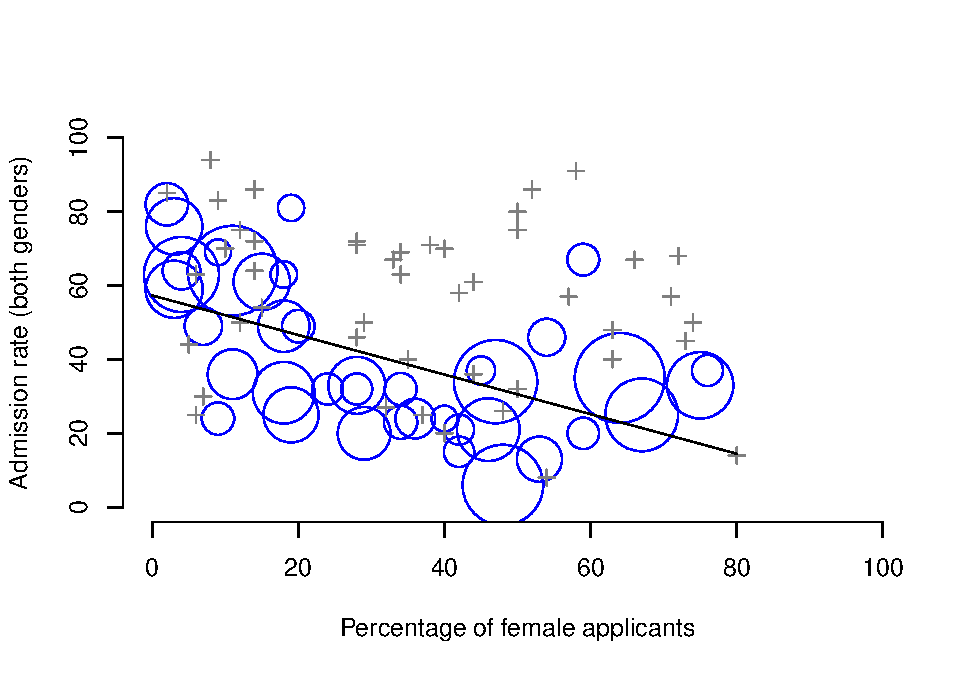
\includegraphics{navarro2_files/figure-latex/berkeley-1.pdf}
\caption{\label{fig:berkeley}The Berkeley 1973 college admissions data. This
figure plots the admission rate for the 85 departments that had at least
one female applicant, as a function of the percentage of applicants that
were female. The plot is a redrawing of Figure 1 from
\citet{Bickel1975}. Circles plot departments with more than 40
applicants; the area of the circle is proportional to the total number
of applicants. The crosses plot department with fewer than 40
applicants.}
\end{figure}

Before leaving this topic entirely, I want to point out something else
really critical that is often overlooked in a research methods class.
Statistics only solves \emph{part} of the problem. Remember that we
started all this with the concern that Berkeley's admissions processes
might be unfairly biased against female applicants. When we looked at
the ``aggregated'' data, it did seem like the university was
discriminating against women, but when we ``disaggregate'' and looked at
the individual behaviour of all the departments, it turned out that the
actual departments were, if anything, slightly biased in favour of
women. The gender bias in total admissions was caused by the fact that
women tended to self-select for harder departments. From a legal
perspective, that would probably put the university in the clear.
Postgraduate admissions are determined at the level of the individual
department (and there are good reasons to do that), and at the level of
individual departments, the decisions are more or less unbiased (the
weak bias in favour of females at that level is small, and not
consistent across departments). Since the university can't dictate which
departments people choose to apply to, and the decision making takes
place at the level of the department it can hardly be held accountable
for any biases that those choices produce.

That was the basis for my somewhat glib remarks earlier, but that's not
exactly the whole story, is it? After all, if we're interested in this
from a more sociological and psychological perspective, we might want to
ask \emph{why} there are such strong gender differences in applications.
Why do males tend to apply to engineering more often than females, and
why is this reversed for the English department? And why is it it the
case that the departments that tend to have a female-application bias
tend to have lower overall admission rates than those departments that
have a male-application bias? Might this not still reflect a gender
bias, even though every single department is itself unbiased? It might.
Suppose, hypothetically, that males preferred to apply to ``hard
sciences'' and females prefer ``humanities''. And suppose further that
the reason for why the humanities departments have low admission rates
is because the government doesn't want to fund the humanities
(Ph.D.~places, for instance, are often tied to government funded
research projects). Does that constitute a gender bias? Or just an
unenlightened view of the value of the humanities? What if someone at a
high level in the government cut the humanities funds because they felt
that the humanities are ``useless chick stuff''. That seems pretty
\emph{blatantly} gender biased. None of this falls within the purview of
statistics, but it matters to the research project. If you're interested
in the overall structural effects of subtle gender biases, then you
probably want to look at \emph{both} the aggregated and disaggregated
data. If you're interested in the decision making process at Berkeley
itself then you're probably only interested in the disaggregated data.

In short there are a lot of critical questions that you can't answer
with statistics, but the answers to those questions will have a huge
impact on how you analyse and interpret data. And this is the reason why
you should always think of statistics as a \emph{tool} to help you learn
about your data, no more and no less. It's a powerful tool to that end,
but there's no substitute for careful thought.

\section{Statistics in psychology}\label{statistics-in-psychology}

I hope that the discussion above helped explain why science in general
is so focused on statistics. But I'm guessing that you have a lot more
questions about what role statistics plays in psychology, and
specifically why psychology classes always devote so many lectures to
stats. So here's my attempt to answer a few of them\ldots{}

\textbf{Why does psychology have so much statistics?}

To be perfectly honest, there's a few different reasons, some of which
are better than others. The most important reason is that psychology is
a statistical science. What I mean by that is that the ``things'' that
we study are \emph{people}. Real, complicated, gloriously messy,
infuriatingly perverse people. The ``things'' of physics include object
like electrons, and while there are all sorts of complexities that arise
in physics, electrons don't have minds of their own. They don't have
opinions, they don't differ from each other in weird and arbitrary ways,
they don't get bored in the middle of an experiment, and they don't get
angry at the experimenter and then deliberately try to sabotage the data
set (not that I've ever done that\ldots{}). At a fundamental level
psychology is harder than physics.\footnote{Which might explain why
  physics is just a teensy bit further advanced as a science than we
  are.}

Basically, we teach statistics to you as psychologists because you need
to be better at stats than physicists. There's actually a saying used
sometimes in physics, to the effect that ``if your experiment needs
statistics, you should have done a better experiment''. They have the
luxury of being able to say that because their objects of study are
pathetically simple in comparison to the vast mess that confronts social
scientists. It's not just psychology, really: most social sciences are
desperately reliant on statistics. Not because we're bad experimenters,
but because we've picked a harder problem to solve. We teach you stats
because you really, really need it.

\textbf{Can't someone else do the statistics?}

To some extent, but not completely. It's true that you don't need to
become a fully trained statistician just to do psychology, but you do
need to reach a certain level of statistical competence. In my view,
there's three reasons that every psychological researcher ought to be
able to do basic statistics:

\begin{itemize}
\tightlist
\item
  Firstly, there's the fundamental reason: statistics is deeply
  intertwined with research design. If you want to be good at designing
  psychological studies, you need to at least understand the basics of
  stats.
\item
  Secondly, if you want to be good at the psychological side of the
  research, then you need to be able to understand the psychological
  literature, right? But almost every paper in the psychological
  literature reports the results of statistical analyses. So if you
  really want to understand the psychology, you need to be able to
  understand what other people did with their data. And that means
  understanding a certain amount of statistics.
\item
  Thirdly, there's a big practical problem with being dependent on other
  people to do all your statistics: statistical analysis is
  \emph{expensive}. If you ever get bored and want to look up how much
  the Australian government charges for university fees, you'll notice
  something interesting: statistics is designated as a ``national
  priority'' category, and so the fees are much, much lower than for any
  other area of study. This is because there's a massive shortage of
  statisticians out there. So, from your perspective as a psychological
  researcher, the laws of supply and demand aren't exactly on your side
  here! As a result, in almost any real life situation where you want to
  do psychological research, the cruel facts will be that you don't have
  enough money to afford a statistician. So the economics of the
  situation mean that you have to be pretty self-sufficient.
\end{itemize}

Note that a lot of these reasons generalise beyond researchers. If you
want to be a practicing psychologist and stay on top of the field, it
helps to be able to read the scientific literature, which relies pretty
heavily on statistics.

\textbf{I don't care about jobs, research, or clinical work. Do I need
statistics?}

Okay, now you're just messing with me. Still, I think it should matter
to you too. Statistics should matter to you in the same way that
statistics should matter to \emph{everyone}: we live in the 21st
century, and data are \emph{everywhere}. Frankly, given the world in
which we live these days, a basic knowledge of statistics is pretty damn
close to a survival tool! Which is the topic of the next section\ldots{}

\section{Statistics in everyday life}\label{statistics-in-everyday-life}

\begin{quote}
\emph{``We are drowning in information,~but we are starved for
knowledge''}

-Various authors, original probably John Naisbitt
\end{quote}

When I started writing up my lecture notes I took the 20 most recent
news articles posted to the ABC news website. Of those 20 articles, it
turned out that 8 of them involved a discussion of something that I
would call a statistical topic; 6 of those made a mistake. The most
common error, if you're curious, was failing to report baseline data
(e.g., the article mentions that 5\% of people in situation X have some
characteristic Y, but doesn't say how common the characteristic is for
everyone else!) The point I'm trying to make here isn't that journalists
are bad at statistics (though they almost always are), it's that a basic
knowledge of statistics is very helpful for trying to figure out when
someone else is either making a mistake or even lying to you. In fact,
one of the biggest things that a knowledge of statistics does to you is
cause you to get angry at the newspaper or the internet on a far more
frequent basis: you can find a good example of this in Section
\ref{housingpriceexample}. In later versions of this book I'll try to
include more anecdotes along those lines.

\section{There's more to research methods than
statistics}\label{theres-more-to-research-methods-than-statistics}

So far, most of what I've talked about is statistics, and so you'd be
forgiven for thinking that statistics is all I care about in life. To be
fair, you wouldn't be far wrong, but research methodology is a broader
concept than statistics. So most research methods courses will cover a
lot of topics that relate much more to the pragmatics of research
design, and in particular the issues that you encounter when trying to
do research with humans. However, about 99\% of student \emph{fears}
relate to the statistics part of the course, so I've focused on the
stats in this discussion, and hopefully I've convinced you that
statistics matters, and more importantly, that it's not to be feared.
That being said, it's pretty typical for introductory research methods
classes to be very stats-heavy. This is not (usually) because the
lecturers are evil people. Quite the contrary, in fact. Introductory
classes focus a lot on the statistics because you almost always find
yourself needing statistics before you need the other research methods
training. Why? Because almost all of your assignments in other classes
will rely on statistical training, to a much greater extent than they
rely on other methodological tools. It's not common for undergraduate
assignments to require you to design your own study from the ground up
(in which case you would need to know a lot about research design), but
it \emph{is} common for assignments to ask you to analyse and interpret
data that were collected in a study that someone else designed (in which
case you need statistics). In that sense, from the perspective of
allowing you to do well in all your other classes, the statistics is
more urgent.

But note that ``urgent'' is different from ``important'' -- they both
matter. I really do want to stress that research design is just as
important as data analysis, and this book does spend a fair amount of
time on it. However, while statistics has a kind of universality, and
provides a set of core tools that are useful for most types of
psychological research, the research methods side isn't quite so
universal. There are some general principles that everyone should think
about, but a lot of research design is very idiosyncratic, and is
specific to the area of research that you want to engage in. To the
extent that it's the details that matter, those details don't usually
show up in an introductory stats and research methods class.

\chapter{A brief introduction to research design}\label{studydesign}

\begin{quote}
\emph{To consult the statistician after an experiment is finished is
often merely to ask him to conduct a post mortem examination. He can
perhaps say what the experiment died of.}

-- Sir Ronald Fisher\footnote{Presidential Address to the First Indian
  Statistical Congress, 1938. Source:
  \url{http://en.wikiquote.org/wiki/Ronald_Fisher}}
\end{quote}

In this chapter, we're going to start thinking about the basic ideas
that go into designing a study, collecting data, checking whether your
data collection works, and so on. It won't give you enough information
to allow you to design studies of your own, but it will give you a lot
of the basic tools that you need to assess the studies done by other
people. However, since the focus of this book is much more on data
analysis than on data collection, I'm only giving a very brief overview.
Note that this chapter is ``special'' in two ways. Firstly, it's much
more psychology-specific than the later chapters. Secondly, it focuses
much more heavily on the scientific problem of research methodology, and
much less on the statistical problem of data analysis. Nevertheless, the
two problems are related to one another, so it's traditional for stats
textbooks to discuss the problem in a little detail. This chapter relies
heavily on \citet{Campbell1963} for the discussion of study design, and
\citet{Stevens1946} for the discussion of scales of measurement. Later
versions will attempt to be more precise in the citations.

\hypertarget{measurement}{\section{Introduction to psychological
measurement}\label{measurement}}

The first thing to understand is data collection can be thought of as a
kind of \textbf{\emph{measurement}}. That is, what we're trying to do
here is measure something about human behaviour or the human mind. What
do I mean by ``measurement''?

\subsection{Some thoughts about psychological
measurement}\label{some-thoughts-about-psychological-measurement}

Measurement itself is a subtle concept, but basically it comes down to
finding some way of assigning numbers, or labels, or some other kind of
well-defined descriptions to ``stuff''. So, any of the following would
count as a psychological measurement:

\begin{itemize}
\tightlist
\item
  My \textbf{age} is \emph{33 years}.
\item
  I \emph{do not} \textbf{like anchovies}.
\item
  My \textbf{chromosomal gender} is \emph{male}.
\item
  My \textbf{self-identified gender} is \emph{male}.\footnote{Well\ldots{}
    now this is awkward, isn't it? This section is one of the oldest
    parts of the book, and it's outdated in a rather embarrassing way. I
    wrote this in 2010, at which point all of those facts \emph{were}
    true. Revisiting this in 2018\ldots{} well I'm not 33 any more, but
    that's not surprising I suppose. I can't imagine my chromosomes have
    changed, so I'm going to guess my karyotype was then and is now XY.
    The self-identified gender, on the other hand\ldots{} ah. I suppose
    the fact that the title page now refers to me as Danielle rather
    than Daniel might possibly be a giveaway, but I don't typically
    identify as ``male'' on a gender questionnaire these days, and I
    prefer \emph{``she/her''} pronouns as a default (it's a long story)!
    I did think a little about how I was going to handle this in the
    book, actually. The book has a somewhat distinct authorial voice to
    it, and I feel like it would be a rather different work if I went
    back and wrote everything as Danielle and updated all the pronouns
    in the work. Besides, it would be a lot of work, so I've left my
    name as ``Dan'' throughout the book, and in ant case ``Dan'' is a
    perfectly good nickname for ``Danielle'', don't you think? In any
    case, it's not a big deal. I only wanted to mention it to make life
    a little easier for readers who aren't sure how to refer to me. I
    still don't like anchovies though :-)}
\end{itemize}

In the short list above, the \textbf{bolded part} is ``the thing to be
measured'', and the \emph{italicised part} is ``the measurement
itself''. In fact, we can expand on this a little bit, by thinking about
the set of possible measurements that could have arisen in each case:

\begin{itemize}
\tightlist
\item
  My \textbf{age} (in years) could have been \emph{0, 1, 2, 3 \ldots{}},
  etc. The upper bound on what my age could possibly be is a bit fuzzy,
  but in practice you'd be safe in saying that the largest possible age
  is \emph{150}, since no human has ever lived that long.
\item
  When asked if I \textbf{like anchovies}, I might have said that
  \emph{I do}, or \emph{I do not}, or \emph{I have no opinion}, or
  \emph{I sometimes do}.
\item
  My \textbf{chromosomal gender} is almost certainly going to be
  \emph{male (XY)} or \emph{female (XX)}, but there are a few other
  possibilities. I could also have \emph{Klinfelter's syndrome (XXY)},
  which is more similar to male than to female. And I imagine there are
  other possibilities too.
\item
  My \textbf{self-identified gender} is also very likely to be
  \emph{male} or \emph{female}, but it doesn't have to agree with my
  chromosomal gender. I may also choose to identify with \emph{neither},
  or to explicitly call myself \emph{transgender}.
\end{itemize}

As you can see, for some things (like age) it seems fairly obvious what
the set of possible measurements should be, whereas for other things it
gets a bit tricky. But I want to point out that even in the case of
someone's age, it's much more subtle than this. For instance, in the
example above, I assumed that it was okay to measure age in years. But
if you're a developmental psychologist, that's way too crude, and so you
often measure age in \emph{years and months} (if a child is 2 years and
11 months, this is usually written as ``2;11''). If you're interested in
newborns, you might want to measure age in \emph{days since birth},
maybe even \emph{hours since birth}. In other words, the way in which
you specify the allowable measurement values is important.

Looking at this a bit more closely, you might also realise that the
concept of ``age'' isn't actually all that precise. In general, when we
say ``age'' we implicitly mean ``the length of time since birth''. But
that's not always the right way to do it. Suppose you're interested in
how newborn babies control their eye movements. If you're interested in
kids that young, you might also start to worry that ``birth'' is not the
only meaningful point in time to care about. If Baby Alice is born 3
weeks premature and Baby Bianca is born 1 week late, would it really
make sense to say that they are the ``same age'' if we encountered them
``2 hours after birth''? In one sense, yes: by social convention, we use
birth as our reference point for talking about age in everyday life,
since it defines the amount of time the person has been operating as an
independent entity in the world, but from a scientific perspective
that's not the only thing we care about. When we think about the biology
of human beings, it's often useful to think of ourselves as organisms
that have been growing and maturing since conception, and from that
perspective Alice and Bianca aren't the same age at all. So you might
want to define the concept of ``age'' in two different ways: the length
of time since conception, and the length of time since birth. When
dealing with adults, it won't make much difference, but when dealing
with newborns it might.

Moving beyond these issues, there's the question of methodology. What
specific ``measurement method'' are you going to use to find out
someone's age? As before, there are lots of different possibilities:

\begin{itemize}
\tightlist
\item
  You could just ask people ``how old are you?'' The method of
  self-report is fast, cheap and easy, but it only works with people old
  enough to understand the question, and some people lie about their
  age.
\item
  You could ask an authority (e.g., a parent) ``how old is your child?''
  This method is fast, and when dealing with kids it's not all that hard
  since the parent is almost always around. It doesn't work as well if
  you want to know ``age since conception'', since a lot of parents
  can't say for sure when conception took place. For that, you might
  need a different authority (e.g., an obstetrician).
\item
  You could look up official records, like birth certificates. This is
  time consuming and annoying, but it has its uses (e.g., if the person
  is now dead).
\end{itemize}

\subsection{Operationalisation: defining your
measurement}\label{operationalisation-defining-your-measurement}

All of the ideas discussed in the previous section all relate to the
concept of \textbf{\emph{operationalisation}}. To be a bit more precise
about the idea, operationalisation is the process by which we take a
meaningful but somewhat vague concept, and turn it into a precise
measurement. The process of operationalisation can involve several
different things:

\begin{itemize}
\tightlist
\item
  Being precise about what you are trying to measure. For instance, does
  ``age'' mean ``time since birth'' or ``time since conception'' in the
  context of your research?
\item
  Determining what method you will use to measure it. Will you use
  self-report to measure age, ask a parent, or look up an official
  record? If you're using self-report, how will you phrase the question?
\item
  Defining the set of the allowable values that the measurement can
  take. Note that these values don't always have to be numerical, though
  they often are. When measuring age, the values are numerical, but we
  still need to think carefully about what numbers are allowed. Do we
  want age in years, years and months, days, hours? Etc. For other types
  of measurements (e.g., gender), the values aren't numerical. But, just
  as before, we need to think about what values are allowed. If we're
  asking people to self-report their gender, what options to we allow
  them to choose between? Is it enough to allow only ``male'' or
  ``female''? Do you need an ``other'' option? Or should we not give
  people any specific options, and let them answer in their own words?
  And if you open up the set of possible values to include all verbal
  response, how will you interpret their answers?
\end{itemize}

Operationalisation is a tricky business, and there's no ``one, true
way'' to do it. The way in which you choose to operationalise the
informal concept of ``age'' or ``gender'' into a formal measurement
depends on what you need to use the measurement for. Often you'll find
that the community of scientists who work in your area have some fairly
well-established ideas for how to go about it. In other words,
operationalisation needs to be thought through on a case by case basis.
Nevertheless, while there a lot of issues that are specific to each
individual research project, there are some aspects to it that are
pretty general.

Before moving on, I want to take a moment to clear up our terminology,
and in the process introduce one more term. Here are four different
things that are closely related to each other:

\begin{itemize}
\tightlist
\item
  \textbf{\emph{A theoretical construct}}. This is the thing that you're
  trying to take a measurement of, like ``age'', ``gender'' or an
  ``opinion''. A theoretical construct can't be directly observed, and
  often they're actually a bit vague.
\item
  \textbf{\emph{A measure}}. The measure refers to the method or the
  tool that you use to make your observations. A question in a survey, a
  behavioural observation or a brain scan could all count as a measure.
\item
  \textbf{\emph{An operationalisation}}. The term ``operationalisation''
  refers to the logical connection between the measure and the
  theoretical construct, or to the process by which we try to derive a
  measure from a theoretical construct.
\item
  \textbf{\emph{A variable}}. Finally, a new term. A variable is what we
  end up with when we apply our measure to something in the world. That
  is, variables are the actual ``data'' that we end up with in our data
  sets.
\end{itemize}

In practice, even scientists tend to blur the distinction between these
things, but it's very helpful to try to understand the differences.

\hypertarget{scales}{\section{Scales of measurement}\label{scales}}

As the previous section indicates, the outcome of a psychological
measurement is called a variable. But not all variables are of the same
qualitative type, and it's very useful to understand what types there
are. A very useful concept for distinguishing between different types of
variables is what's known as \textbf{\emph{scales of measurement}}.

\subsection{Nominal scale}\label{nominal-scale}

A \textbf{\emph{nominal scale}} variable (also referred to as a
\textbf{\emph{categorical}} variable) is one in which there is no
particular relationship between the different possibilities: for these
kinds of variables it doesn't make any sense to say that one of them is
``bigger' or''better" than any other one, and it absolutely doesn't make
any sense to average them. The classic example for this is ``eye
colour''. Eyes can be blue, green and brown, among other possibilities,
but none of them is any ``better'' than any other one. As a result, it
would feel really weird to talk about an ``average eye colour''.
Similarly, gender is nominal too: male isn't better or worse than
female, neither does it make sense to try to talk about an ``average
gender''. In short, nominal scale variables are those for which the only
thing you can say about the different possibilities is that they are
different. That's it.

Let's take a slightly closer look at this. Suppose I was doing research
on how people commute to and from work. One variable I would have to
measure would be what kind of transportation people use to get to work.
This ``transport type'' variable could have quite a few possible values,
including: ``train'', ``bus'', ``car'', ``bicycle'', etc. For now, let's
suppose that these four are the only possibilities, and suppose that
when I ask 100 people how they got to work today, and I get this:

\begin{longtable}[]{@{}cc@{}}
\toprule
Transportation & Number of people\tabularnewline
\midrule
\endhead
(1) Train & 12\tabularnewline
(2) Bus & 30\tabularnewline
(3) Car & 48\tabularnewline
(4) Bicycle & 10\tabularnewline
\bottomrule
\end{longtable}

So, what's the average transportation type? Obviously, the answer here
is that there isn't one. It's a silly question to ask. You can say that
travel by car is the most popular method, and travel by train is the
least popular method, but that's about all. Similarly, notice that the
order in which I list the options isn't very interesting. I could have
chosen to display the data like this

\begin{longtable}[]{@{}cc@{}}
\toprule
Transportation & Number of people\tabularnewline
\midrule
\endhead
(3) Car & 48\tabularnewline
(1) Train & 12\tabularnewline
(4) Bicycle & 10\tabularnewline
(2) Bus & 30\tabularnewline
\bottomrule
\end{longtable}

and nothing really changes.

\subsection{Ordinal scale}\label{ordinal-scale}

\textbf{\emph{Ordinal scale}} variables have a bit more structure than
nominal scale variables, but not by a lot. An ordinal scale variable is
one in which there is a natural, meaningful way to order the different
possibilities, but you can't do anything else. The usual example given
of an ordinal variable is ``finishing position in a race''. You
\emph{can} say that the person who finished first was faster than the
person who finished second, but you \emph{don't} know how much faster.
As a consequence we know that 1st \textgreater{} 2nd, and we know that
2nd \textgreater{} 3rd, but the difference between 1st and 2nd might be
much larger than the difference between 2nd and 3rd.

Here's an more psychologically interesting example. Suppose I'm
interested in people's attitudes to climate change, and I ask them to
pick one of these four statements that most closely matches their
beliefs:

\begin{quote}
\begin{enumerate}
\def\labelenumi{(\arabic{enumi})}
\tightlist
\item
  Temperatures are rising, because of human activity
\item
  Temperatures are rising, but we don't know why
\item
  Temperatures are rising, but not because of humans
\item
  Temperatures are not rising
\end{enumerate}
\end{quote}

Notice that these four statements actually do have a natural ordering,
in terms of ``the extent to which they agree with the current science''.
Statement 1 is a close match, statement 2 is a reasonable match,
statement 3 isn't a very good match, and statement 4 is in strong
opposition to the science. So, in terms of the thing I'm interested in
(the extent to which people endorse the science), I can order the items
as 1 \textgreater{} 2 \textgreater{} 3 \textgreater{} 4. Since this
ordering exists, it would be very weird to list the options like
this\ldots{}

\begin{quote}
\begin{enumerate}
\def\labelenumi{(\arabic{enumi})}
\setcounter{enumi}{2}
\tightlist
\item
  Temperatures are rising, but not because of humans
\item
  Temperatures are rising, because of human activity
\item
  Temperatures are not rising
\item
  Temperatures are rising, but we don't know why
\end{enumerate}
\end{quote}

\ldots{} because it seems to violate the natural ``structure'' to the
question.

So, let's suppose I asked 100 people these questions, and got the
following answers:

\begin{longtable}[]{@{}lc@{}}
\toprule
Response & Number\tabularnewline
\midrule
\endhead
(1) Temperatures are rising, because of human activity &
51\tabularnewline
(2) Temperatures are rising, but we don't know why & 20\tabularnewline
(3) Temperatures are rising, but not because of humans &
10\tabularnewline
(4) Temperatures are not rising & 19\tabularnewline
\bottomrule
\end{longtable}

When analysing these data, it seems quite reasonable to try to group
(1), (2) and (3) together, and say that 81 of 100 people were willing to
\emph{at least partially} endorse the science. And it's \emph{also}
quite reasonable to group (2), (3) and (4) together and say that 49 of
100 people registered \emph{at least some disagreement} with the
dominant scientific view. However, it would be entirely bizarre to try
to group (1), (2) and (4) together and say that 90 of 100 people
said\ldots{} what? There's nothing sensible that allows you to group
those responses together at all.

That said, notice that while we \emph{can} use the natural ordering of
these items to construct sensible groupings, what we \emph{can't} do is
average them. For instance, in my simple example here, the ``average''
response to the question is 1.97. If you can tell me what that means,
I'd love to know. Because that sounds like gibberish to me!

\subsection{Interval scale}\label{interval-scale}

In contrast to nominal and ordinal scale variables,
\textbf{\emph{interval scale}} and ratio scale variables are variables
for which the numerical value is genuinely meaningful. In the case of
interval scale variables, the \emph{differences} between the numbers are
interpretable, but the variable doesn't have a ``natural'' zero value. A
good example of an interval scale variable is measuring temperature in
degrees celsius. For instance, if it was 15\(^\circ\) yesterday and
18\(^\circ\) today, then the 3\(^\circ\) difference between the two is
genuinely meaningful. Moreover, that 3\(^\circ\) difference is
\emph{exactly the same} as the 3\(^\circ\) difference between
7\(^\circ\) and 10\(^\circ\). In short, addition and subtraction are
meaningful for interval scale variables.\footnote{Actually, I've been
  informed by readers with greater physics knowledge than I that
  temperature isn't strictly an interval scale, in the sense that the
  amount of energy required to heat something up by 3\(^\circ\) depends
  on it's current temperature. So in the sense that physicists care
  about, temperature isn't actually interval scale. But it still makes a
  cute example, so I'm going to ignore this little inconvenient truth.}

However, notice that the 0\(^\circ\) does not mean ``no temperature at
all'': it actually means ``the temperature at which water freezes'',
which is pretty arbitrary. As a consequence, it becomes pointless to try
to multiply and divide temperatures. It is wrong to say that
\(20^\circ\) is \emph{twice as hot} as 10\(^\circ\), just as it is weird
and meaningless to try to claim that 20\(^\circ\) is negative two times
as hot as -10\(^\circ\).

Again, lets look at a more psychological example. Suppose I'm interested
in looking at how the attitudes of first-year university students have
changed over time. Obviously, I'm going to want to record the year in
which each student started. This is an interval scale variable. A
student who started in 2003 did arrive 5 years before a student who
started in 2008. However, it would be completely insane for me to divide
2008 by 2003 and say that the second student started ``1.0024 times
later'' than the first one. That doesn't make any sense at all.

\subsection{Ratio scale}\label{ratio-scale}

The fourth and final type of variable to consider is a
\textbf{\emph{ratio scale}} variable, in which zero really means zero,
and it's okay to multiply and divide. A good psychological example of a
ratio scale variable is response time (RT). In a lot of tasks it's very
common to record the amount of time somebody takes to solve a problem or
answer a question, because it's an indicator of how difficult the task
is. Suppose that Alan takes 2.3 seconds to respond to a question,
whereas Ben takes 3.1 seconds. As with an interval scale variable,
addition and subtraction are both meaningful here. Ben really did take
3.1 - 2.3 = 0.8 seconds longer than Alan did. However, notice that
multiplication and division also make sense here too: Ben took 3.1 / 2.3
= 1.35 times as long as Alan did to answer the question. And the reason
why you can do this is that, for a ratio scale variable such as RT,
``zero seconds'' really does mean ``no time at all''.

\subsection{Continuous versus discrete
variables}\label{continuousdiscrete}

There's a second kind of distinction that you need to be aware of,
regarding what types of variables you can run into. This is the
distinction between continuous variables and discrete variables. The
difference between these is as follows:

\begin{itemize}
\tightlist
\item
  A \textbf{\emph{continuous variable}} is one in which, for any two
  values that you can think of, it's always logically possible to have
  another value in between.
\item
  A \textbf{\emph{discrete variable}} is, in effect, a variable that
  isn't continuous. For a discrete variable, it's sometimes the case
  that there's nothing in the middle.
\end{itemize}

These definitions probably seem a bit abstract, but they're pretty
simple once you see some examples. For instance, response time is
continuous. If Alan takes 3.1 seconds and Ben takes 2.3 seconds to
respond to a question, then it's possible for Cameron's response time to
lie in between, by taking 3.0 seconds. And of course it would also be
possible for David to take 3.031 seconds to respond, meaning that his RT
would lie in between Cameron's and Alan's. And while in practice it
might be impossible to measure RT that precisely, it's certainly
possible in principle. Because we can always find a new value for RT in
between any two other ones, we say that RT is continuous.

Discrete variables occur when this rule is violated. For example,
nominal scale variables are always discrete: there isn't a type of
transportation that falls ``in between'' trains and bicycles, not in the
strict mathematical way that 2.3 falls in between 2 and 3. So
transportation type is discrete. Similarly, ordinal scale variables are
always discrete: although ``2nd place'' does fall between ``1st place''
and ``3rd place'', there's nothing that can logically fall in between
``1st place'' and ``2nd place''. Interval scale and ratio scale
variables can go either way. As we saw above, response time (a ratio
scale variable) is continuous. Temperature in degrees celsius (an
interval scale variable) is also continuous. However, the year you went
to school (an interval scale variable) is discrete. There's no year in
between 2002 and 2003. The number of questions you get right on a
true-or-false test (a ratio scale variable) is also discrete: since a
true-or-false question doesn't allow you to be ``partially correct'',
there's nothing in between 5/10 and 6/10. Table \ref{tab:scalescont}
summarises the relationship between the scales of measurement and the
discrete/continuity distinction. Cells with a tick mark correspond to
things that are possible. I'm trying to hammer this point home, because
(a) some textbooks get this wrong, and (b) people very often say things
like ``discrete variable'' when they mean ``nominal scale variable''.
It's very unfortunate.

\begin{table}

\caption{\label{tab:scalescont}The relationship between the scales of measurement and the discrete/continuity distinction. Cells with a tick mark correspond to things that are possible.}
\centering
\begin{tabular}[t]{lcclcclcc}
\toprule
 & continuous & discrete\\
nominal &  & \$\textbackslash{}checkmark\$\\
ordinal &  & \$\textbackslash{}checkmark\$\\
interval & \$\textbackslash{}checkmark\$ & \$\textbackslash{}checkmark\$\\
ratio & \$\textbackslash{}checkmark\$ & \$\textbackslash{}checkmark\$\\
\bottomrule
\end{tabular}
\end{table}

\subsection{Some complexities}\label{some-complexities}

Okay, I know you're going to be shocked to hear this, but \ldots{} the
real world is much messier than this little classification scheme
suggests. Very few variables in real life actually fall into these nice
neat categories, so you need to be kind of careful not to treat the
scales of measurement as if they were hard and fast rules. It doesn't
work like that: they're guidelines, intended to help you think about the
situations in which you should treat different variables differently.
Nothing more.

So let's take a classic example, maybe \emph{the} classic example, of a
psychological measurement tool: the \textbf{\emph{Likert scale}}. The
humble Likert scale is the bread and butter tool of all survey design.
You yourself have filled out hundreds, maybe thousands of them, and odds
are you've even used one yourself. Suppose we have a survey question
that looks like this:

\begin{quote}
Which of the following best describes your opinion of the statement that
``all pirates are freaking awesome'' \ldots{}
\end{quote}

and then the options presented to the participant are these:

\begin{quote}
\begin{enumerate}
\def\labelenumi{(\arabic{enumi})}
\tightlist
\item
  Strongly disagree
\item
  Disagree
\item
  Neither agree nor disagree
\item
  Agree
\item
  Strongly agree
\end{enumerate}
\end{quote}

This set of items is an example of a 5-point Likert scale: people are
asked to choose among one of several (in this case 5) clearly ordered
possibilities, generally with a verbal descriptor given in each case.
However, it's not necessary that all items be explicitly described. This
is a perfectly good example of a 5-point Likert scale too:

\begin{quote}
\begin{enumerate}
\def\labelenumi{(\arabic{enumi})}
\item
  Strongly disagree
\item
\item
\item
\item
  Strongly agree
\end{enumerate}
\end{quote}

Likert scales are very handy, if somewhat limited, tools. The question
is, what kind of variable are they? They're obviously discrete, since
you can't give a response of 2.5. They're obviously not nominal scale,
since the items are ordered; and they're not ratio scale either, since
there's no natural zero.

But are they ordinal scale or interval scale? One argument says that we
can't really prove that the difference between ``strongly agree'' and
``agree'' is of the same size as the difference between ``agree'' and
``neither agree nor disagree''. In fact, in everyday life it's pretty
obvious that they're not the same at all. So this suggests that we ought
to treat Likert scales as ordinal variables. On the other hand, in
practice most participants do seem to take the whole ``on a scale from 1
to 5'' part fairly seriously, and they tend to act as if the differences
between the five response options were fairly similar to one another. As
a consequence, a lot of researchers treat Likert scale data as if it
were interval scale. It's not interval scale, but in practice it's close
enough that we usually think of it as being \textbf{\emph{quasi-interval
scale}}.

\hypertarget{reliability}{\section{Assessing the reliability of a
measurement}\label{reliability}}

At this point we've thought a little bit about how to operationalise a
theoretical construct and thereby create a psychological measure; and
we've seen that by applying psychological measures we end up with
variables, which can come in many different types. At this point, we
should start discussing the obvious question: is the measurement any
good? We'll do this in terms of two related ideas: \emph{reliability}
and \emph{validity}. Put simply, the \textbf{\emph{reliability}} of a
measure tells you how \emph{precisely} you are measuring something,
whereas the validity of a measure tells you how \emph{accurate} the
measure is. In this section I'll talk about reliability; we'll talk
about validity in the next chapter.

Reliability is actually a very simple concept: it refers to the
repeatability or consistency of your measurement. The measurement of my
weight by means of a ``bathroom scale'' is very reliable: if I step on
and off the scales over and over again, it'll keep giving me the same
answer. Measuring my intelligence by means of ``asking my mum'' is very
unreliable: some days she tells me I'm a bit thick, and other days she
tells me I'm a complete moron. Notice that this concept of reliability
is different to the question of whether the measurements are correct
(the correctness of a measurement relates to it's validity). If I'm
holding a sack of potatos when I step on and off of the bathroom scales,
the measurement will still be reliable: it will always give me the same
answer. However, this highly reliable answer doesn't match up to my true
weight at all, therefore it's wrong. In technical terms, this is a
\emph{reliable but invalid} measurement. Similarly, while my mum's
estimate of my intelligence is a bit unreliable, she might be right.
Maybe I'm just not too bright, and so while her estimate of my
intelligence fluctuates pretty wildly from day to day, it's basically
right. So that would be an \emph{unreliable but valid} measure. Of
course, to some extent, notice that if my mum's estimates are too
unreliable, it's going to be very hard to figure out which one of her
many claims about my intelligence is actually the right one. To some
extent, then, a very unreliable measure tends to end up being invalid
for practical purposes; so much so that many people would say that
reliability is necessary (but not sufficient) to ensure validity.

Okay, now that we're clear on the distinction between reliability and
validity, let's have a think about the different ways in which we might
measure reliability:

\begin{itemize}
\tightlist
\item
  \textbf{\emph{Test-retest reliability}}. This relates to consistency
  over time: if we repeat the measurement at a later date, do we get a
  the same answer?
\item
  \textbf{\emph{Inter-rater reliability}}. This relates to consistency
  across people: if someone else repeats the measurement (e.g., someone
  else rates my intelligence) will they produce the same answer?
\item
  \textbf{\emph{Parallel forms reliability}}. This relates to
  consistency across theoretically-equivalent measurements: if I use a
  different set of bathroom scales to measure my weight, does it give
  the same answer?
\item
  \textbf{\emph{Internal consistency reliability}}. If a measurement is
  constructed from lots of different parts that perform similar
  functions (e.g., a personality questionnaire result is added up across
  several questions) do the individual parts tend to give similar
  answers.
\end{itemize}

Not all measurements need to possess all forms of reliability. For
instance, educational assessment can be thought of as a form of
measurement. One of the subjects that I teach, \emph{Computational
Cognitive Science}, has an assessment structure that has a research
component and an exam component (plus other things). The exam component
is \emph{intended} to measure something different from the research
component, so the assessment as a whole has low internal consistency.
However, within the exam there are several questions that are intended
to (approximately) measure the same things, and those tend to produce
similar outcomes; so the exam on its own has a fairly high internal
consistency. Which is as it should be. You should only demand
reliability in those situations where you want to be measure the same
thing!

\hypertarget{ivdv}{\section{\texorpdfstring{The ``role'' of variables:
predictors and
outcomes}{The role of variables: predictors and outcomes}}\label{ivdv}}

Okay, I've got one last piece of terminology that I need to explain to
you before moving away from variables. Normally, when we do some
research we end up with lots of different variables. Then, when we
analyse our data we usually try to explain some of the variables in
terms of some of the other variables. It's important to keep the two
roles ``thing doing the explaining'' and ``thing being explained''
distinct. So let's be clear about this now. Firstly, we might as well
get used to the idea of using mathematical symbols to describe
variables, since it's going to happen over and over again. Let's denote
the ``to be explained'' variable \(Y\), and denote the variables ``doing
the explaining'' as \(X_1\), \(X_2\), etc.

Now, when we doing an analysis, we have different names for \(X\) and
\(Y\), since they play different roles in the analysis. The classical
names for these roles are \textbf{\emph{independent variable}} (IV) and
\textbf{\emph{dependent variable}} (DV). The IV is the variable that you
use to do the explaining (i.e., \(X\)) and the DV is the variable being
explained (i.e., \(Y\)). The logic behind these names goes like this: if
there really is a relationship between \(X\) and \(Y\) then we can say
that \(Y\) depends on \(X\), and if we have designed our study
``properly'' then \(X\) isn't dependent on anything else. However, I
personally find those names horrible: they're hard to remember and
they're highly misleading, because (a) the IV is never actually
``independent of everything else'' and (b) if there's no relationship,
then the DV doesn't actually depend on the IV. And in fact, because I'm
not the only person who thinks that IV and DV are just awful names,
there are a number of alternatives that I find more appealing. The terms
that I'll use in these notes are \textbf{\emph{predictors}} and
\textbf{\emph{outcomes}}. The idea here is that what you're trying to do
is use \(X\) (the predictors) to make guesses about \(Y\) (the
outcomes).\footnote{Annoyingly, though, there's a lot of different names
  used out there. I won't list all of them -- there would be no point in
  doing that -- other than to note that R often uses ``response
  variable'' where I've used ``outcome'', and a traditionalist would use
  ``dependent variable''. Sigh. This sort of terminological confusion is
  very common, I'm afraid.} This is summarised in Table \ref{tab:ivdv}.

\begin{table}

\caption{\label{tab:ivdv}The terminology used to distinguish between different roles that a variable can play when analysing a data set. Note that this book will tend to avoid the classical terminology in favour of the newer names.}
\centering
\begin{tabular}[t]{lll}
\toprule
role of the variable & classical name & modern name\\
\midrule
to be explained & dependent variable (DV) & outcome\\
to do the explaining & independent variable (IV) & predictor\\
\bottomrule
\end{tabular}
\end{table}

\hypertarget{researchdesigns}{\section{Experimental and non-experimental
research}\label{researchdesigns}}

One of the big distinctions that you should be aware of is the
distinction between ``experimental research'' and ``non-experimental
research''. When we make this distinction, what we're really talking
about is the degree of control that the researcher exercises over the
people and events in the study.

\subsection{Experimental research}\label{experimental-research}

The key features of \textbf{\emph{experimental research}} is that the
researcher controls all aspects of the study, especially what
participants experience during the study. In particular, the researcher
manipulates or varies the predictor variables (IVs), and then allows the
outcome variable (DV) to vary naturally. The idea here is to
deliberately vary the predictors (IVs) to see if they have any causal
effects on the outcomes. Moreover, in order to ensure that there's no
chance that something other than the predictor variables is causing the
outcomes, everything else is kept constant or is in some other way
``balanced'' to ensure that they have no effect on the results. In
practice, it's almost impossible to \emph{think} of everything else that
might have an influence on the outcome of an experiment, much less keep
it constant. The standard solution to this is
\textbf{\emph{randomisation}}: that is, we randomly assign people to
different groups, and then give each group a different treatment (i.e.,
assign them different values of the predictor variables). We'll talk
more about randomisation later in this course, but for now, it's enough
to say that what randomisation does is minimise (but not eliminate) the
chances that there are any systematic difference between groups.

Let's consider a very simple, completely unrealistic and grossly
unethical example. Suppose you wanted to find out if smoking causes lung
cancer. One way to do this would be to find people who smoke and people
who don't smoke, and look to see if smokers have a higher rate of lung
cancer. This is \emph{not} a proper experiment, since the researcher
doesn't have a lot of control over who is and isn't a smoker. And this
really matters: for instance, it might be that people who choose to
smoke cigarettes also tend to have poor diets, or maybe they tend to
work in asbestos mines, or whatever. The point here is that the groups
(smokers and non-smokers) actually differ on lots of things, not
\emph{just} smoking. So it might be that the higher incidence of lung
cancer among smokers is caused by something else, not by smoking per se.
In technical terms, these other things (e.g.~diet) are called
``confounds'', and we'll talk about those in just a moment.

In the meantime, let's now consider what a proper experiment might look
like. Recall that our concern was that smokers and non-smokers might
differ in lots of ways. The solution, as long as you have no ethics, is
to \emph{control} who smokes and who doesn't. Specifically, if we
randomly divide participants into two groups, and force half of them to
become smokers, then it's very unlikely that the groups will differ in
any respect other than the fact that half of them smoke. That way, if
our smoking group gets cancer at a higher rate than the non-smoking
group, then we can feel pretty confident that (a) smoking does cause
cancer and (b) we're murderers.

\subsection{Non-experimental research}\label{non-experimental-research}

\textbf{\emph{Non-experimental research}} is a broad term that covers
``any study in which the researcher doesn't have quite as much control
as they do in an experiment''. Obviously, control is something that
scientists like to have, but as the previous example illustrates, there
are lots of situations in which you can't or shouldn't try to obtain
that control. Since it's grossly unethical (and almost certainly
criminal) to force people to smoke in order to find out if they get
cancer, this is a good example of a situation in which you really
shouldn't try to obtain experimental control. But there are other
reasons too. Even leaving aside the ethical issues, our ``smoking
experiment'' does have a few other issues. For instance, when I
suggested that we ``force'' half of the people to become smokers, I must
have been talking about \emph{starting} with a sample of non-smokers,
and then forcing them to become smokers. While this sounds like the kind
of solid, evil experimental design that a mad scientist would love, it
might not be a very sound way of investigating the effect in the real
world. For instance, suppose that smoking only causes lung cancer when
people have poor diets, and suppose also that people who normally smoke
do tend to have poor diets. However, since the ``smokers'' in our
experiment aren't ``natural'' smokers (i.e., we forced non-smokers to
become smokers; they didn't take on all of the other normal, real life
characteristics that smokers might tend to possess) they probably have
better diets. As such, in this silly example they wouldn't get lung
cancer, and our experiment will fail, because it violates the structure
of the ``natural'' world (the technical name for this is an
``artifactual'' result; see later).

One distinction worth making between two types of non-experimental
research is the difference between \textbf{\emph{quasi-experimental
research}} and \textbf{\emph{case studies}}. The example I discussed
earlier -- in which we wanted to examine incidence of lung cancer among
smokers and non-smokers, without trying to control who smokes and who
doesn't -- is a quasi-experimental design. That is, it's the same as an
experiment, but we don't control the predictors (IVs). We can still use
statistics to analyse the results, it's just that we have to be a lot
more careful.

The alternative approach, case studies, aims to provide a very detailed
description of one or a few instances. In general, you can't use
statistics to analyse the results of case studies, and it's usually very
hard to draw any general conclusions about ``people in general'' from a
few isolated examples. However, case studies are very useful in some
situations. Firstly, there are situations where you don't have any
alternative: neuropsychology has this issue a lot. Sometimes, you just
can't find a lot of people with brain damage in a specific area, so the
only thing you can do is describe those cases that you do have in as
much detail and with as much care as you can. However, there's also some
genuine advantages to case studies: because you don't have as many
people to study, you have the ability to invest lots of time and effort
trying to understand the specific factors at play in each case. This is
a very valuable thing to do. As a consequence, case studies can
complement the more statistically-oriented approaches that you see in
experimental and quasi-experimental designs. We won't talk much about
case studies in these lectures, but they are nevertheless very valuable
tools!

\hypertarget{validity}{\section{Assessing the validity of a
study}\label{validity}}

More than any other thing, a scientist wants their research to be
``valid''. The conceptual idea behind \textbf{\emph{validity}} is very
simple: can you trust the results of your study? If not, the study is
invalid. However, while it's easy to state, in practice it's much harder
to check validity than it is to check reliability. And in all honesty,
there's no precise, clearly agreed upon notion of what validity actually
is. In fact, there's lots of different kinds of validity, each of which
raises it's own issues, and not all forms of validity are relevant to
all studies. I'm going to talk about five different types:

\begin{itemize}
\tightlist
\item
  Internal validity
\item
  External validity
\item
  Construct validity
\item
  Face validity
\item
  Ecological validity
\end{itemize}

To give you a quick guide as to what matters here\ldots{} (1) Internal
and external validity are the most important, since they tie directly to
the fundamental question of whether your study really works. (2)
Construct validity asks whether you're measuring what you think you are.
(3) Face validity isn't terribly important except insofar as you care
about ``appearances''. (4) Ecological validity is a special case of face
validity that corresponds to a kind of appearance that you might care
about a lot.

\subsection{Internal validity}\label{internal-validity}

\textbf{\emph{Internal validity}} refers to the extent to which you are
able draw the correct conclusions about the causal relationships between
variables. It's called ``internal'' because it refers to the
relationships between things ``inside'' the study. Let's illustrate the
concept with a simple example. Suppose you're interested in finding out
whether a university education makes you write better. To do so, you get
a group of first year students, ask them to write a 1000 word essay, and
count the number of spelling and grammatical errors they make. Then you
find some third-year students, who obviously have had more of a
university education than the first-years, and repeat the exercise. And
let's suppose it turns out that the third-year students produce fewer
errors. And so you conclude that a university education improves writing
skills. Right? Except\ldots{} the big problem that you have with this
experiment is that the third-year students are older, and they've had
more experience with writing things. So it's hard to know for sure what
the causal relationship is: Do older people write better? Or people who
have had more writing experience? Or people who have had more education?
Which of the above is the true \emph{cause} of the superior performance
of the third-years? Age? Experience? Education? You can't tell. This is
an example of a failure of internal validity, because your study doesn't
properly tease apart the \emph{causal} relationships between the
different variables.

\subsection{External validity}\label{external-validity}

\textbf{\emph{External validity}} relates to the
\textbf{\emph{generalisability}} of your findings. That is, to what
extent do you expect to see the same pattern of results in ``real life''
as you saw in your study. To put it a bit more precisely, any study that
you do in psychology will involve a fairly specific set of questions or
tasks, will occur in a specific environment, and will involve
participants that are drawn from a particular subgroup. So, if it turns
out that the results don't actually generalise to people and situations
beyond the ones that you studied, then what you've got is a lack of
external validity.

The classic example of this issue is the fact that a very large
proportion of studies in psychology will use undergraduate psychology
students as the participants. Obviously, however, the researchers don't
care \emph{only} about psychology students; they care about people in
general. Given that, a study that uses only psych students as
participants always carries a risk of lacking external validity. That
is, if there's something ``special'' about psychology students that
makes them different to the general populace in some \emph{relevant}
respect, then we may start worrying about a lack of external validity.

That said, it is absolutely critical to realise that a study that uses
only psychology students does not necessarily have a problem with
external validity. I'll talk about this again later, but it's such a
common mistake that I'm going to mention it here. The external validity
is threatened by the choice of population if (a) the population from
which you sample your participants is very narrow (e.g., psych
students), and (b) the narrow population that you sampled from is
systematically different from the general population, \emph{in some
respect that is relevant to the psychological phenomenon that you intend
to study}. The italicised part is the bit that lots of people forget: it
is true that psychology undergraduates differ from the general
population in lots of ways, and so a study that uses only psych students
\emph{may} have problems with external validity. However, if those
differences aren't very relevant to the phenomenon that you're studying,
then there's nothing to worry about. To make this a bit more concrete,
here's two extreme examples:

\begin{itemize}
\tightlist
\item
  You want to measure ``attitudes of the general public towards
  psychotherapy'', but all of your participants are psychology students.
  This study would almost certainly have a problem with external
  validity.
\item
  You want to measure the effectiveness of a visual illusion, and your
  participants are all psychology students. This study is very unlikely
  to have a problem with external validity
\end{itemize}

Having just spent the last couple of paragraphs focusing on the choice
of participants (since that's the big issue that everyone tends to worry
most about), it's worth remembering that external validity is a broader
concept. The following are also examples of things that might pose a
threat to external validity, depending on what kind of study you're
doing:

\begin{itemize}
\tightlist
\item
  People might answer a ``psychology questionnaire'' in a manner that
  doesn't reflect what they would do in real life.
\item
  Your lab experiment on (say) ``human learning'' has a different
  structure to the learning problems people face in real life.
\end{itemize}

\subsection{Construct validity}\label{construct-validity}

\textbf{\emph{Construct validity}} is basically a question of whether
you're measuring what you want to be measuring. A measurement has good
construct validity if it is actually measuring the correct theoretical
construct, and bad construct validity if it doesn't. To give very simple
(if ridiculous) example, suppose I'm trying to investigate the rates
with which university students cheat on their exams. And the way I
attempt to measure it is by asking the cheating students to stand up in
the lecture theatre so that I can count them. When I do this with a
class of 300 students, 0 people claim to be cheaters. So I therefore
conclude that the proportion of cheaters in my class is 0\%. Clearly
this is a bit ridiculous. But the point here is not that this is a very
deep methodological example, but rather to explain what construct
validity is. The problem with my measure is that while I'm \emph{trying}
to measure ``the proportion of people who cheat'' what I'm actually
measuring is ``the proportion of people stupid enough to own up to
cheating, or bloody minded enough to pretend that they do''. Obviously,
these aren't the same thing! So my study has gone wrong, because my
measurement has very poor construct validity.

\subsection{Face validity}\label{face-validity}

\textbf{\emph{Face validity}} simply refers to whether or not a measure
``looks like'' it's doing what it's supposed to, nothing more. If I
design a test of intelligence, and people look at it and they say ``no,
that test doesn't measure intelligence'', then the measure lacks face
validity. It's as simple as that. Obviously, face validity isn't very
important from a pure scientific perspective. After all, what we care
about is whether or not the measure \emph{actually} does what it's
supposed to do, not whether it \emph{looks like} it does what it's
supposed to do. As a consequence, we generally don't care very much
about face validity. That said, the concept of face validity serves
three useful pragmatic purposes:

\begin{itemize}
\tightlist
\item
  Sometimes, an experienced scientist will have a ``hunch'' that a
  particular measure won't work. While these sorts of hunches have no
  strict evidentiary value, it's often worth paying attention to them.
  Because often times people have knowledge that they can't quite
  verbalise, so there might be something to worry about even if you
  can't quite say why. In other words, when someone you trust criticises
  the face validity of your study, it's worth taking the time to think
  more carefully about your design to see if you can think of reasons
  why it might go awry. Mind you, if you don't find any reason for
  concern, then you should probably not worry: after all, face validity
  really doesn't matter much.
\item
  Often (very often), completely uninformed people will also have a
  ``hunch'' that your research is crap. And they'll criticise it on the
  internet or something. On close inspection, you'll often notice that
  these criticisms are actually focused entirely on how the study
  ``looks'', but not on anything deeper. The concept of face validity is
  useful for gently explaining to people that they need to substantiate
  their arguments further.
\item
  Expanding on the last point, if the beliefs of untrained people are
  critical (e.g., this is often the case for applied research where you
  actually want to convince policy makers of something or other) then
  you \emph{have} to care about face validity. Simply because -- whether
  you like it or not -- a lot of people will use face validity as a
  proxy for real validity. If you want the government to change a law on
  scientific, psychological grounds, then it won't matter how good your
  studies ``really'' are. If they lack face validity, you'll find that
  politicians ignore you. Of course, it's somewhat unfair that policy
  often depends more on appearance than fact, but that's how things go.
\end{itemize}

\subsection{Ecological validity}\label{ecological-validity}

\textbf{\emph{Ecological validity}} is a different notion of validity,
which is similar to external validity, but less important. The idea is
that, in order to be ecologically valid, the entire set up of the study
should closely approximate the real world scenario that is being
investigated. In a sense, ecological validity is a kind of face validity
-- it relates mostly to whether the study ``looks'' right, but with a
bit more rigour to it. To be ecologically valid, the study has to look
right in a fairly specific way. The idea behind it is the intuition that
a study that is ecologically valid is more likely to be externally
valid. It's no guarantee, of course. But the nice thing about ecological
validity is that it's much easier to check whether a study is
ecologically valid than it is to check whether a study is externally
valid. An simple example would be eyewitness identification studies.
Most of these studies tend to be done in a university setting, often
with fairly simple array of faces to look at rather than a line up. The
length of time between seeing the ``criminal'' and being asked to
identify the suspect in the ``line up'' is usually shorter. The
``crime'' isn't real, so there's no chance that the witness being
scared, and there's no police officers present, so there's not as much
chance of feeling pressured. These things all mean that the study
\emph{definitely} lacks ecological validity. They might (but might not)
mean that it also lacks external validity.

\section{Confounds, artifacts and other threats to
validity}\label{confounds-artifacts-and-other-threats-to-validity}

If we look at the issue of validity in the most general fashion, the two
biggest worries that we have are \emph{confounds} and \emph{artifact}.
These two terms are defined in the following way:

\begin{itemize}
\tightlist
\item
  \textbf{\emph{Confound}}: A confound is an additional, often
  unmeasured variable\footnote{The reason why I say that it's unmeasured
    is that if you \emph{have} measured it, then you can use some fancy
    statistical tricks to deal with the confound. Because of the
    existence of these statistical solutions to the problem of
    confounds, we often refer to a confound that we have measured and
    dealt with as a \emph{covariate}. Dealing with covariates is a topic
    for a more advanced course, but I thought I'd mention it in passing,
    since it's kind of comforting to at least know that this stuff
    exists.} that turns out to be related to both the predictors and the
  outcomes. The existence of confounds threatens the internal validity
  of the study because you can't tell whether the predictor causes the
  outcome, or if the confounding variable causes it, etc.
\item
  \textbf{\emph{Artifact}}: A result is said to be ``artifactual'' if it
  only holds in the special situation that you happened to test in your
  study. The possibility that your result is an artifact describes a
  threat to your external validity, because it raises the possibility
  that you can't generalise your results to the actual population that
  you care about.
\end{itemize}

As a general rule confounds are a bigger concern for non-experimental
studies, precisely because they're not proper experiments: by
definition, you're leaving lots of things uncontrolled, so there's a lot
of scope for confounds working their way into your study. Experimental
research tends to be much less vulnerable to confounds: the more control
you have over what happens during the study, the more you can prevent
confounds from appearing.

However, there's always swings and roundabouts, and when we start
thinking about artifacts rather than confounds, the shoe is very firmly
on the other foot. For the most part, artifactual results tend to be a
concern for experimental studies than for non-experimental studies. To
see this, it helps to realise that the reason that a lot of studies are
non-experimental is precisely because what the researcher is trying to
do is examine human behaviour in a more naturalistic context. By working
in a more real-world context, you lose experimental control (making
yourself vulnerable to confounds) but because you tend to be studying
human psychology ``in the wild'' you reduce the chances of getting an
artifactual result. Or, to put it another way, when you take psychology
out of the wild and bring it into the lab (which we usually have to do
to gain our experimental control), you always run the risk of
accidentally studying something different than you wanted to study:
which is more or less the definition of an artifact.

Be warned though: the above is a rough guide only. It's absolutely
possible to have confounds in an experiment, and to get artifactual
results with non-experimental studies. This can happen for all sorts of
reasons, not least of which is researcher error. In practice, it's
really hard to think everything through ahead of time, and even very
good researchers make mistakes. But other times it's unavoidable, simply
because the researcher has ethics (e.g., see ``differential
attrition'').

Okay. There's a sense in which almost any threat to validity can be
characterised as a confound or an artifact: they're pretty vague
concepts. So let's have a look at some of the most common
examples\ldots{}

\subsection{History effects}\label{history-effects}

\textbf{\emph{History effects}} refer to the possibility that specific
events may occur during the study itself that might influence the
outcomes. For instance, something might happen in between a pre-test and
a post-test. Or, in between testing participant 23 and participant 24.
Alternatively, it might be that you're looking at an older study, which
was perfectly valid for its time, but the world has changed enough since
then that the conclusions are no longer trustworthy. Examples of things
that would count as history effects:

\begin{itemize}
\tightlist
\item
  You're interested in how people think about risk and uncertainty. You
  started your data collection in December 2010. But finding
  participants and collecting data takes time, so you're still finding
  new people in February 2011. Unfortunately for you (and even more
  unfortunately for others), the Queensland floods occurred in January
  2011, causing billions of dollars of damage and killing many people.
  Not surprisingly, the people tested in February 2011 express quite
  different beliefs about handling risk than the people tested in
  December 2010. Which (if any) of these reflects the ``true'' beliefs
  of participants? I think the answer is probably both: the Queensland
  floods genuinely changed the beliefs of the Australian public, though
  possibly only temporarily. The key thing here is that the ``history''
  of the people tested in February is quite different to people tested
  in December.
\item
  You're testing the psychological effects of a new anti-anxiety drug.
  So what you do is measure anxiety before administering the drug (e.g.,
  by self-report, and taking physiological measures, let's say), then
  you administer the drug, and then you take the same measures
  afterwards. In the middle, however, because your labs are in Los
  Angeles, there's an earthquake, which increases the anxiety of the
  participants.
\end{itemize}

\subsection{Maturation effects}\label{maturation-effects}

As with history effects, \textbf{\emph{maturational effects}} are
fundamentally about change over time. However, maturation effects aren't
in response to specific events. Rather, they relate to how people change
on their own over time: we get older, we get tired, we get bored, etc.
Some examples of maturation effects:

\begin{itemize}
\tightlist
\item
  When doing developmental psychology research, you need to be aware
  that children grow up quite rapidly. So, suppose that you want to find
  out whether some educational trick helps with vocabulary size among 3
  year olds. One thing that you need to be aware of is that the
  vocabulary size of children that age is growing at an incredible rate
  (multiple words per day), all on its own. If you design your study
  without taking this maturational effect into account, then you won't
  be able to tell if your educational trick works.
\item
  When running a very long experiment in the lab (say, something that
  goes for 3 hours), it's very likely that people will begin to get
  bored and tired, and that this maturational effect will cause
  performance to decline, regardless of anything else going on in the
  experiment
\end{itemize}

\subsection{Repeated testing effects}\label{repeated-testing-effects}

An important type of history effect is the effect of
\textbf{\emph{repeated testing}}. Suppose I want to take two
measurements of some psychological construct (e.g., anxiety). One thing
I might be worried about is if the first measurement has an effect on
the second measurement. In other words, this is a history effect in
which the ``event'' that influences the second measurement is the first
measurement itself! This is not at all uncommon. Examples of this
include:

\begin{itemize}
\tightlist
\item
  \emph{Learning and practice}: e.g., ``intelligence'' at time 2 might
  appear to go up relative to time 1 because participants learned the
  general rules of how to solve ``intelligence-test-style'' questions
  during the first testing session.\\
\item
  \emph{Familiarity with the testing situation}: e.g., if people are
  nervous at time 1, this might make performance go down; after sitting
  through the first testing situation, they might calm down a lot
  precisely because they've seen what the testing looks like.
\item
  \emph{Auxiliary changes caused by testing}: e.g., if a questionnaire
  assessing mood is boring, then mood at measurement at time 2 is more
  likely to become ``bored'', precisely because of the boring
  measurement made at time 1.
\end{itemize}

\subsection{Selection bias}\label{selection-bias}

\textbf{\emph{Selection bias}} is a pretty broad term. Suppose that
you're running an experiment with two groups of participants, where each
group gets a different ``treatment'', and you want to see if the
different treatments lead to different outcomes. However, suppose that,
despite your best efforts, you've ended up with a gender imbalance
across groups (say, group A has 80\% females and group B has 50\%
females). It might sound like this could never happen, but trust me, it
can. This is an example of a selection bias, in which the people
``selected into'' the two groups have different characteristics. If any
of those characteristics turns out to be relevant (say, your treatment
works better on females than males) then you're in a lot of trouble.

\subsection{Differential attrition}\label{differential-attrition}

One quite subtle danger to be aware of is called
\textbf{\emph{differential attrition}}, which is a kind of selection
bias that is caused by the study itself. Suppose that, for the first
time ever in the history of psychology, I manage to find the perfectly
balanced and representative sample of people. I start running ``Dan's
incredibly long and tedious experiment'' on my perfect sample, but then,
because my study is incredibly long and tedious, lots of people start
dropping out. I can't stop this: as we'll discuss later in the chapter
on research ethics, participants absolutely have the right to stop doing
any experiment, any time, for whatever reason they feel like, and as
researchers we are morally (and professionally) obliged to remind people
that they do have this right. So, suppose that ``Dan's incredibly long
and tedious experiment'' has a very high drop out rate. What do you
suppose the odds are that this drop out is random? Answer: zero. Almost
certainly, the people who remain are more conscientious, more tolerant
of boredom etc than those that leave. To the extent that (say)
conscientiousness is relevant to the psychological phenomenon that I
care about, this attrition can decrease the validity of my results.

When thinking about the effects of differential attrition, it is
sometimes helpful to distinguish between two different types. The first
is \textbf{\emph{homogeneous attrition}}, in which the attrition effect
is the same for all groups, treatments or conditions. In the example I
gave above, the differential attrition would be homogeneous if (and only
if) the easily bored participants are dropping out of all of the
conditions in my experiment at about the same rate. In general, the main
effect of homogeneous attrition is likely to be that it makes your
sample unrepresentative. As such, the biggest worry that you'll have is
that the generalisability of the results decreases: in other words, you
lose external validity.

The second type of differential attrition is \textbf{\emph{heterogeneous
attrition}}, in which the attrition effect is different for different
groups. This is a much bigger problem: not only do you have to worry
about your external validity, you also have to worry about your internal
validity too. To see why this is the case, let's consider a very dumb
study in which I want to see if insulting people makes them act in a
more obedient way. Why anyone would actually want to study that I don't
know, but let's suppose I really, deeply cared about this. So, I design
my experiment with two conditions. In the ``treatment'' condition, the
experimenter insults the participant and then gives them a questionnaire
designed to measure obedience. In the ``control'' condition, the
experimenter engages in a bit of pointless chitchat and then gives them
the questionnaire. Leaving aside the questionable scientific merits and
dubious ethics of such a study, let's have a think about what might go
wrong here. As a general rule, when someone insults me to my face, I
tend to get much less co-operative. So, there's a pretty good chance
that a lot more people are going to drop out of the treatment condition
than the control condition. And this drop out isn't going to be random.
The people most likely to drop out would probably be the people who
don't care all that much about the importance of obediently sitting
through the experiment. Since the most bloody minded and disobedient
people all left the treatment group but not the control group, we've
introduced a confound: the people who actually took the questionnaire in
the treatment group were \emph{already} more likely to be dutiful and
obedient than the people in the control group. In short, in this study
insulting people doesn't make them more obedient: it makes the more
disobedient people leave the experiment! The internal validity of this
experiment is completely shot.

\subsection{Non-response bias}\label{non-response-bias}

\textbf{\emph{Non-response bias}} is closely related to selection bias,
and to differential attrition. The simplest version of the problem goes
like this. You mail out a survey to 1000 people, and only 300 of them
reply. The 300 people who replied are almost certainly not a random
subsample. People who respond to surveys are systematically different to
people who don't. This introduces a problem when trying to generalise
from those 300 people who replied, to the population at large; since you
now have a very non-random sample. The issue of non-response bias is
more general than this, though. Among the (say) 300 people that did
respond to the survey, you might find that not everyone answers every
question. If (say) 80 people chose not to answer one of your questions,
does this introduce problems? As always, the answer is maybe. If the
question that wasn't answered was on the last page of the questionnaire,
and those 80 surveys were returned with the last page missing, there's a
good chance that the missing data isn't a big deal: probably the pages
just fell off. However, if the question that 80 people didn't answer was
the most confrontational or invasive personal question in the
questionnaire, then almost certainly you've got a problem. In essence,
what you're dealing with here is what's called the problem of
\textbf{\emph{missing data}}. If the data that is missing was ``lost''
randomly, then it's not a big problem. If it's missing systematically,
then it can be a big problem.

\subsection{Regression to the mean}\label{regression-to-the-mean}

\textbf{\emph{Regression to the mean}} is a curious variation on
selection bias. It refers to any situation where you select data based
on an extreme value on some measure. Because the measure has natural
variation, it almost certainly means that when you take a subsequent
measurement, that later measurement will be less extreme than the first
one, purely by chance.

Here's an example. Suppose I'm interested in whether a psychology
education has an adverse effect on very smart kids. To do this, I find
the 20 psych I students with the best high school grades and look at how
well they're doing at university. It turns out that they're doing a lot
better than average, but they're not topping the class at university,
even though they did top their classes at high school. What's going on?
The natural first thought is that this must mean that the psychology
classes must be having an adverse effect on those students. However,
while that might very well be the explanation, it's more likely that
what you're seeing is an example of ``regression to the mean''. To see
how it works, let's take a moment to think about what is required to get
the best mark in a class, regardless of whether that class be at high
school or at university. When you've got a big class, there are going to
be \emph{lots} of very smart people enrolled. To get the best mark you
have to be very smart, work very hard, and be a bit lucky. The exam has
to ask just the right questions for your idiosyncratic skills, and you
have to not make any dumb mistakes (we all do that sometimes) when
answering them. And that's the thing: intelligence and hard work are
transferrable from one class to the next. Luck isn't. The people who got
lucky in high school won't be the same as the people who get lucky at
university. That's the very definition of ``luck''. The consequence of
this is that, when you select people at the very extreme values of one
measurement (the top 20 students), you're selecting for hard work, skill
and luck. But because the luck doesn't transfer to the second
measurement (only the skill and work), these people will all be expected
to drop a little bit when you measure them a second time (at
university). So their scores fall back a little bit, back towards
everyone else. This is regression to the mean.

Regression to the mean is surprisingly common. For instance, if two very
tall people have kids, their children will tend to be taller than
average, but not as tall as the parents. The reverse happens with very
short parents: two very short parents will tend to have short children,
but nevertheless those kids will tend to be taller than the parents. It
can also be extremely subtle. For instance, there have been studies done
that suggested that people learn better from negative feedback than from
positive feedback. However, the way that people tried to show this was
to give people positive reinforcement whenever they did good, and
negative reinforcement when they did bad. And what you see is that after
the positive reinforcement, people tended to do worse; but after the
negative reinforcement they tended to do better. But! Notice that
there's a selection bias here: when people do very well, you're
selecting for ``high'' values, and so you should \emph{expect} (because
of regression to the mean) that performance on the next trial should be
worse, regardless of whether reinforcement is given. Similarly, after a
bad trial, people will tend to improve all on their own. The apparent
superiority of negative feedback is an artifact caused by regression to
the mean \citep[see][ for discussion]{Kahneman1973}.

\subsection{Experimenter bias}\label{experimenter-bias}

\textbf{\emph{Experimenter bias}} can come in multiple forms. The basic
idea is that the experimenter, despite the best of intentions, can
accidentally end up influencing the results of the experiment by subtly
communicating the ``right answer'' or the ``desired behaviour'' to the
participants. Typically, this occurs because the experimenter has
special knowledge that the participant does not -- either the right
answer to the questions being asked, or knowledge of the expected
pattern of performance for the condition that the participant is in, and
so on. The classic example of this happening is the case study of
``Clever Hans'', which dates back to 1907
\citep{Pfungst1911, Hothersall2004}. Clever Hans was a horse that
apparently was able to read and count, and perform other human like
feats of intelligence. After Clever Hans became famous, psychologists
started examining his behaviour more closely. It turned out that -- not
surprisingly -- Hans didn't know how to do maths. Rather, Hans was
responding to the human observers around him. Because they did know how
to count, and the horse had learned to change its behaviour when people
changed theirs.

The general solution to the problem of experimenter bias is to engage in
double blind studies, where neither the experimenter nor the participant
knows which condition the participant is in, or knows what the desired
behaviour is. This provides a very good solution to the problem, but
it's important to recognise that it's not quite ideal, and hard to pull
off perfectly. For instance, the obvious way that I could try to
construct a double blind study is to have one of my Ph.D.~students (one
who doesn't know anything about the experiment) run the study. That
feels like it should be enough. The only person (me) who knows all the
details (e.g., correct answers to the questions, assignments of
participants to conditions) has no interaction with the participants,
and the person who does all the talking to people (the Ph.D.~student)
doesn't know anything. Except, that last part is very unlikely to be
true. In order for the Ph.D.~student to run the study effectively, they
need to have been briefed by me, the researcher. And, as it happens, the
Ph.D.~student also knows me, and knows a bit about my general beliefs
about people and psychology (e.g., I tend to think humans are much
smarter than psychologists give them credit for). As a result of all
this, it's almost impossible for the experimenter to avoid knowing a
little bit about what expectations I have. And even a little bit of
knowledge can have an effect: suppose the experimenter accidentally
conveys the fact that the participants are expected to do well in this
task. Well, there's a thing called the ``Pygmalion effect'': if you
expect great things of people, they'll rise to the occasion; but if you
expect them to fail, they'll do that too. In other words, the
expectations become a self-fulfilling prophesy.

\subsection{Demand effects and
reactivity}\label{demand-effects-and-reactivity}

When talking about experimenter bias, the worry is that the
experimenter's knowledge or desires for the experiment are communicated
to the participants, and that these effect people's behaviour
\citep{Rosenthal1966}. However, even if you manage to stop this from
happening, it's almost impossible to stop people from knowing that
they're part of a psychological study. And the mere fact of knowing that
someone is watching/studying you can have a pretty big effect on
behaviour. This is generally referred to as \textbf{\emph{reactivity}}
or \textbf{\emph{demand effects}}. The basic idea is captured by the
Hawthorne effect: people alter their performance because of the
attention that the study focuses on them. The effect takes its name from
a the ``Hawthorne Works'' factory outside of Chicago
\citep[see][]{Adair1984}. A study done in the 1920s looking at the
effects of lighting on worker productivity at the factory turned out to
be an effect of the fact that the workers knew they were being studied,
rather than the lighting.

To get a bit more specific about some of the ways in which the mere fact
of being in a study can change how people behave, it helps to think like
a social psychologist and look at some of the \emph{roles} that people
might adopt during an experiment, but might not adopt if the
corresponding events were occurring in the real world:

\begin{itemize}
\tightlist
\item
  The \emph{good participant} tries to be too helpful to the researcher:
  he or she seeks to figure out the experimenter's hypotheses and
  confirm them.
\item
  The \emph{negative participant} does the exact opposite of the good
  participant: he or she seeks to break or destroy the study or the
  hypothesis in some way.
\item
  The \emph{faithful participant} is unnaturally obedient: he or she
  seeks to follow instructions perfectly, regardless of what might have
  happened in a more realistic setting.
\item
  The \emph{apprehensive participant} gets nervous about being tested or
  studied, so much so that his or her behaviour becomes highly
  unnatural, or overly socially desirable.
\end{itemize}

\subsection{Placebo effects}\label{placebo-effects}

The \textbf{\emph{placebo effect}} is a specific type of demand effect
that we worry a lot about. It refers to the situation where the mere
fact of being treated causes an improvement in outcomes. The classic
example comes from clinical trials: if you give people a completely
chemically inert drug and tell them that it's a cure for a disease, they
will tend to get better faster than people who aren't treated at all. In
other words, it is people's belief that they are being treated that
causes the improved outcomes, not the drug.

\subsection{Situation, measurement and subpopulation
effects}\label{situation-measurement-and-subpopulation-effects}

In some respects, these terms are a catch-all term for ``all other
threats to external validity''. They refer to the fact that the choice
of subpopulation from which you draw your participants, the location,
timing and manner in which you run your study (including who collects
the data) and the tools that you use to make your measurements might all
be influencing the results. Specifically, the worry is that these things
might be influencing the results in such a way that the results won't
generalise to a wider array of people, places and measures.

\subsection{Fraud, deception and
self-deception}\label{fraud-deception-and-self-deception}

\begin{quote}
\emph{It is difficult to get a man to understand something, when his
salary depends on his not understanding it.}

-- Upton Sinclair
\end{quote}

One final thing that I feel like I should mention. While reading what
the textbooks often have to say about assessing the validity of the
study, I couldn't help but notice that they seem to make the assumption
that the researcher is honest. I find this hilarious. While the vast
majority of scientists are honest, in my experience at least, some are
not.\footnote{Some people might argue that if you're not honest then
  you're not a real scientist. Which does have some truth to it I guess,
  but that's disingenuous (google the ``No true Scotsman'' fallacy). The
  fact is that there are lots of people who are employed ostensibly as
  scientists, and whose work has all of the trappings of science, but
  who are outright fraudulent. Pretending that they don't exist by
  saying that they're not scientists is just childish.} Not only that,
as I mentioned earlier, scientists are not immune to belief bias -- it's
easy for a researcher to end up deceiving themselves into believing the
wrong thing, and this can lead them to conduct subtly flawed research,
and then hide those flaws when they write it up. So you need to consider
not only the (probably unlikely) possibility of outright fraud, but also
the (probably quite common) possibility that the research is
unintentionally ``slanted''. I opened a few standard textbooks and
didn't find much of a discussion of this problem, so here's my own
attempt to list a few ways in which these issues can arise are:

\begin{itemize}
\tightlist
\item
  \textbf{\emph{Data fabrication}}. Sometimes, people just make up the
  data. This is occasionally done with ``good'' intentions. For
  instance, the researcher believes that the fabricated data do reflect
  the truth, and may actually reflect ``slightly cleaned up'' versions
  of actual data. On other occasions, the fraud is deliberate and
  malicious. Some high-profile examples where data fabrication has been
  alleged or shown include Cyril Burt (a psychologist who is thought to
  have fabricated some of his data), Andrew Wakefield (who has been
  accused of fabricating his data connecting the MMR vaccine to autism)
  and Hwang Woo-suk (who falsified a lot of his data on stem cell
  research).\\
\item
  \textbf{\emph{Hoaxes}}. Hoaxes share a lot of similarities with data
  fabrication, but they differ in the intended purpose. A hoax is often
  a joke, and many of them are intended to be (eventually) discovered.
  Often, the point of a hoax is to discredit someone or some field.
  There's quite a few well known scientific hoaxes that have occurred
  over the years (e.g., Piltdown man) some of were deliberate attempts
  to discredit particular fields of research (e.g., the Sokal affair).
\item
  \textbf{\emph{Data misrepresentation}}. While fraud gets most of the
  headlines, it's much more common in my experience to see data being
  misrepresented. When I say this, I'm not referring to newspapers
  getting it wrong (which they do, almost always). I'm referring to the
  fact that often, the data don't actually say what the researchers
  think they say. My guess is that, almost always, this isn't the result
  of deliberate dishonesty, it's due to a lack of sophistication in the
  data analyses. For instance, think back to the example of Simpson's
  paradox that I discussed in the beginning of these notes. It's very
  common to see people present ``aggregated'' data of some kind; and
  sometimes, when you dig deeper and find the raw data yourself, you
  find that the aggregated data tell a different story to the
  disaggregated data. Alternatively, you might find that some aspect of
  the data is being hidden, because it tells an inconvenient story
  (e.g., the researcher might choose not to refer to a particular
  variable). There's a lot of variants on this; many of which are very
  hard to detect.
\item
  \textbf{\emph{Study ``misdesign''}}. Okay, this one is subtle.
  Basically, the issue here is that a researcher designs a study that
  has built-in flaws, and those flaws are never reported in the paper.
  The data that are reported are completely real, and are correctly
  analysed, but they are produced by a study that is actually quite
  wrongly put together. The researcher really wants to find a particular
  effect, and so the study is set up in such a way as to make it
  ``easy'' to (artifactually) observe that effect. One sneaky way to do
  this -- in case you're feeling like dabbling in a bit of fraud
  yourself -- is to design an experiment in which it's obvious to the
  participants what they're ``supposed'' to be doing, and then let
  reactivity work its magic for you. If you want, you can add all the
  trappings of double blind experimentation etc. It won't make a
  difference, since the study materials themselves are subtly telling
  people what you want them to do. When you write up the results, the
  fraud won't be obvious to the reader: what's obvious to the
  participant when they're in the experimental context isn't always
  obvious to the person reading the paper. Of course, the way I've
  described this makes it sound like it's always fraud: probably there
  are cases where this is done deliberately, but in my experience the
  bigger concern has been with unintentional misdesign. The researcher
  \emph{believes} \ldots{} and so the study just happens to end up with
  a built in flaw, and that flaw then magically erases itself when the
  study is written up for publication.
\item
  \textbf{\emph{Data mining \& post hoc hypothesising}}. Another way in
  which the authors of a study can more or less lie about what they
  found is by engaging in what's referred to as ``data mining''. As
  we'll discuss later in the class, if you keep trying to analyse your
  data in lots of different ways, you'll eventually find something that
  ``looks'' like a real effect but isn't. This is referred to as ``data
  mining''. It used to be quite rare because data analysis used to take
  weeks, but now that everyone has very powerful statistical software on
  their computers, it's becoming very common. Data mining per se isn't
  ``wrong'', but the more that you do it, the bigger the risk you're
  taking. The thing that is wrong, and I suspect is very common, is
  \emph{unacknowledged} data mining. That is, the researcher run every
  possible analysis known to humanity, finds the one that works, and
  then pretends that this was the only analysis that they ever
  conducted. Worse yet, they often ``invent'' a hypothesis after looking
  at the data, to cover up the data mining. To be clear: it's not wrong
  to change your beliefs after looking at the data, and to reanalyse
  your data using your new ``post hoc'' hypotheses. What is wrong (and,
  I suspect, common) is failing to acknowledge that you've done so. If
  you acknowledge that you did it, then other researchers are able to
  take your behaviour into account. If you don't, then they can't. And
  that makes your behaviour deceptive. Bad!
\item
  \textbf{\emph{Publication bias \& self-censoring}}. Finally, a
  pervasive bias is ``non-reporting'' of negative results. This is
  almost impossible to prevent. Journals don't publish every article
  that is submitted to them: they prefer to publish articles that find
  ``something''. So, if 20 people run an experiment looking at whether
  reading \emph{Finnegans Wake} causes insanity in humans, and 19 of
  them find that it doesn't, which one do you think is going to get
  published? Obviously, it's the one study that did find that
  \emph{Finnegans Wake} causes insanity \footnote{Clearly, the real
    effect is that only insane people would even try to read
    \emph{Finnegans Wake.}}. This is an example of a \emph{publication
  bias}: since no-one ever published the 19 studies that didn't find an
  effect, a naive reader would never know that they existed. Worse yet,
  most researchers ``internalise'' this bias, and end up
  \emph{self-censoring} their research. Knowing that negative results
  aren't going to be accepted for publication, they never even try to
  report them. As a friend of mine says ``for every experiment that you
  get published, you also have 10 failures''. And she's right. The catch
  is, while some (maybe most) of those studies are failures for boring
  reasons (e.g.~you stuffed something up) others might be genuine
  ``null'' results that you ought to acknowledge when you write up the
  ``good'' experiment. And telling which is which is often hard to do. A
  good place to start is a paper by \citet{Ioannidis2005} with the
  depressing title ``Why most published research findings are false''.
  I'd also suggest taking a look at work by \citet{Kuhberger2014}
  presenting statistical evidence that this actually happens in
  psychology.
\end{itemize}

There's probably a lot more issues like this to think about, but that'll
do to start with. What I really want to point out is the blindingly
obvious truth that real world science is conducted by actual humans, and
only the most gullible of people automatically assumes that everyone
else is honest and impartial. Actual scientists aren't usually
\emph{that} naive, but for some reason the world likes to pretend that
we are, and the textbooks we usually write seem to reinforce that
stereotype.

\section{Summary}\label{summary}

This chapter isn't really meant to provide a comprehensive discussion of
psychological research methods: it would require another volume just as
long as this one to do justice to the topic. However, in real life
statistics and study design are tightly intertwined, so it's very handy
to discuss some of the key topics. In this chapter, I've briefly
discussed the following topics:

\begin{itemize}
\tightlist
\item
  \protect\hyperlink{measurement}{Introduction to psychological
  measurement}. What does it mean to operationalise a theoretical
  construct? What does it mean to have variables and take measurements?
\item
  \protect\hyperlink{scales}{Scales of measurement and types of
  variables}. Remember that there are \emph{two} different distinctions
  here: there's the difference between discrete and continuous data, and
  there's the difference between the four different scale types
  (nominal, ordinal, interval and ratio).
\item
  \protect\hyperlink{reliability}{Reliability of a measurement}. If I
  measure the ``same'' thing twice, should I expect to see the same
  result? Only if my measure is reliable. But what does it mean to talk
  about doing the ``same'' thing? Well, that's why we have different
  types of reliability. Make sure you remember what they are.
\item
  \protect\hyperlink{ivdv}{Terminology: predictors and outcomes}. What
  roles do variables play in an analysis? Can you remember the
  difference between predictors and outcomes? Dependent and independent
  variables? Etc.
\item
  \protect\hyperlink{researchdesigns}{Experimental and non-experimental
  research designs}. What makes an experiment an experiment? Is it a
  nice white lab coat, or does it have something to do with researcher
  control over variables?
\item
  \protect\hyperlink{validity}{Validity and its threats}. Does your
  study measure what you want it to? How might things go wrong? And is
  it my imagination, or was that a very long list of possible ways in
  which things can go wrong?
\end{itemize}

All this should make clear to you that study design is a critical part
of research methodology. I built this chapter from the classic little
book by \citet{Campbell1963}, but there are of course a large number of
textbooks out there on research design. Spend a few minutes with your
favourite search engine and you'll find dozens.

\chapter*{Part II. An introduction to
R}\label{part-ii.-an-introduction-to-r}
\addcontentsline{toc}{chapter}{Part II. An introduction to R}

\chapter{Getting started with R}\label{introR}

\begin{quote}
\emph{Robots are nice to work with.}

--Roger Zelazny\footnote{Source: \emph{Dismal Light} (1968).}
\end{quote}

In this chapter I'll discuss how to get started in R. I'll briefly talk
about how to download and install R, but most of the chapter will be
focused on getting you started typing R commands. Our goal in this
chapter is not to learn any statistical concepts: we're just trying to
learn the basics of how R works and get comfortable interacting with the
system. To do this, we'll spend a bit of time using R as a simple
calculator, since that's the easiest thing to do with R. In doing so,
you'll get a bit of a feel for what it's like to work in R. From there
I'll introduce some very basic programming ideas: in particular, I'll
talk about the idea of defining \emph{variables} to store information,
and a few things that you can do with these variables.

However, before going into any of the specifics, it's worth talking a
little about why you might want to use R at all. Given that you're
reading this, you've probably got your own reasons. However, if those
reasons are ``because that's what my stats class uses'', it might be
worth explaining a little why your lecturer has chosen to use R for the
class. Of course, I don't really know why \emph{other} people choose R,
so I'm really talking about why I use it.

\begin{itemize}
\tightlist
\item
  It's sort of obvious, but worth saying anyway: doing your statistics
  on a computer is faster, easier and more powerful than doing
  statistics by hand. Computers excel at mindless repetitive tasks, and
  a lot of statistical calculations are both mindless and repetitive.
  For most people, the only reason to ever do statistical calculations
  with pencil and paper is for learning purposes. In my class I do
  occasionally suggest doing some calculations that way, but the only
  real value to it is pedagogical. It does help you to get a ``feel''
  for statistics to do some calculations yourself, so it's worth doing
  it once. But only once!
\item
  Doing statistics in a spreadsheet (e.g., Microsoft Excel) is generally
  a bad idea in the long run. Although many people are likely feel more
  familiar with them, spreadsheets are very limited in terms of what
  analyses they allow you do. If you get into the habit of trying to do
  your real life data analysis using spreadsheets, then you've dug
  yourself into a very deep hole.
\item
  Avoiding proprietary software is a very good idea. There are a lot of
  commercial packages out there that you can buy, some of which I like
  and some of which I don't. They're usually very glossy in their
  appearance, and generally very powerful (much more powerful than
  spreadsheets). However, they're also very expensive: usually, the
  company sells ``student versions'' (crippled versions of the real
  thing) very cheaply; they sell full powered ``educational versions''
  at a price that makes me wince; and they sell commercial licences with
  a staggeringly high price tag. The business model here is to suck you
  in during your student days, and then leave you dependent on their
  tools when you go out into the real world. It's hard to blame them for
  trying, but personally I'm not in favour of shelling out thousands of
  dollars if I can avoid it. And you can avoid it: if you make use of
  packages like R that are open source and free, you never get trapped
  having to pay exorbitant licensing fees.
\item
  Something that you might not appreciate now, but will love later on if
  you do anything involving data analysis, is the fact that R is highly
  extensible. When you download and install R, you get all the basic
  ``packages'', and those are very powerful on their own. However,
  because R is so open and so widely used, it's become something of a
  standard tool in statistics, and so lots of people write their own
  packages that extend the system. And these are freely available too.
  One of the consequences of this, I've noticed, is that if you open up
  an advanced textbook (a recent one, that is) rather than introductory
  textbooks, is that a \emph{lot} of them use R. In other words, if you
  learn how to do your basic statistics in R, then you're a lot closer
  to being able to use the state of the art methods than you would be if
  you'd started out with a ``simpler'' system: so if you want to become
  a genuine expert in psychological data analysis, learning R is a very
  good use of your time.
\item
  Related to the previous point: R is a real programming language. As
  you get better at using R for data analysis, you're also learning to
  program. To some people this might seem like a bad thing, but in
  truth, programming is a core research skill across a lot of the social
  and behavioural sciences. Think about how many surveys and experiments
  are done online, or presented on computers. Think about all those
  online social environments which you might be interested in studying;
  and maybe collecting data from in an automated fashion. Think about
  artificial intelligence systems, computer vision and speech
  recognition. If any of these are things that you think you might want
  to be involved in -- as someone ``doing research in psychology'', that
  is -- you'll need to know a bit of programming. And if you don't
  already know how to program, then learning how to do statistics using
  R is a nice way to start.
\end{itemize}

Those are the main reasons I use R. It's not without its flaws: it's not
easy to learn, and it has a few very annoying quirks to it that we're
all pretty much stuck with, but on the whole I think the strengths
outweigh the weakness; more so than any other option I've encountered so
far.

\hypertarget{gettingR}{\section{Installing R}\label{gettingR}}

Okay, enough with the sales pitch. Let's get started. Just as with any
piece of software, R needs to be installed on a ``computer'', which is a
magical box that does cool things and delivers free ponies. Or something
along those lines: I may be confusing computers with the iPad marketing
campaigns. Anyway, R is freely distributed online, and you can download
it from the R homepage, which is:

\begin{quote}
\url{http://cran.r-project.org/}
\end{quote}

At the top of the page -- under the heading ``Download and Install R''
-- you'll see separate links for Windows users, Mac users, and Linux
users. If you follow the relevant link, you'll see that the online
instructions are pretty self-explanatory, but I'll walk you through the
installation anyway. As of this writing, the current version of R is
3.0.2 (``Frisbee Sailing``), but they usually issue updates every six
months, so you'll probably have a newer version.\footnote{Although R is
  updated frequently, it doesn't usually make much of a difference for
  the sort of work we'll do in this book. In fact, during the writing of
  the book I upgraded several times, and didn't have to change much
  except these sections describing the downloading.}

\subsection{Installing R on a Windows
computer}\label{installing-r-on-a-windows-computer}

The CRAN homepage changes from time to time, and it's not particularly
pretty, or all that well-designed quite frankly. But it's not difficult
to find what you're after. In general you'll find a link at the top of
the page with the text ``Download R for Windows''. If you click on that,
it will take you to a page that offers you a few options. Again, at the
very top of the page you'll be told to click on a link that says to
click here if you're installing R for the first time. That's probably
what you want. This will take you to a page that has a prominent link at
the top called ``Download R 3.0.2 for Windows''. That's the one you
want. Click on that and your browser should start downloading a file
called \texttt{R-3.0.2-win.exe}, or whatever the equivalent version
number is by the time you read this. The file for version 3.0.2 is about
54MB in size, so it may take some time depending on how fast your
internet connection is. Once you've downloaded the file, double click to
install it. As with any software you download online, Windows will ask
you some questions about whether you trust the file and so on. After you
click through those, it'll ask you where you want to install it, and
what components you want to install. The default values should be fine
for most people, so again, just click through. Once all that is done,
you should have R installed on your system. You can access it from the
Start menu, or from the desktop if you asked it to add a shortcut there.
You can now open up R in the usual way if you want to, but what I'm
going to suggest is that instead of doing that you should now install
RStudio.

\subsection{Installing R on a Mac}\label{installing-r-on-a-mac}

When you click on the Mac OS X link, you should find yourself on a page
with the title ``R for Mac OS X''. The vast majority of Mac users will
have a fairly recent version of the operating system: as long as you're
running Mac OS X 10.6 (Snow Leopard) or higher, then you'll be
fine.\footnote{If you're running an older version of the Mac OS, then
  you need to follow the link to the ``old'' page
  (\url{http://cran.r-project.org/bin/macosx/old/}). You should be able
  to find the installer file that you need at the bottom of the page.}
There's a fairly prominent link on the page called ``R-3.0.2.pkg'',
which is the one you want. Click on that link and you'll start
downloading the installer file, which is (not surprisingly) called
\texttt{R-3.0.2.pkg}. It's about 61MB in size, so the download can take
a while on slower internet connections.

Once you've downloaded \texttt{R-3.0.2.pkg}, all you need to do is open
it by double clicking on the package file. The installation should go
smoothly from there: just follow all the instructions just like you
usually do when you install something. Once it's finished, you'll find a
file called \texttt{R.app} in the Applications folder. You can now open
up R in the usual way\footnote{Tip for advanced Mac users. You can run R
  from the terminal if you want to. The command is just ``R''. It
  behaves like the normal desktop version, except that help
  documentation behaves like a ``man'' page instead of opening in a new
  window.} if you want to, but what I'm going to suggest is that instead
of doing that you should now install RStudio.

\subsection{Installing R on a Linux
computer}\label{installing-r-on-a-linux-computer}

If you're successfully managing to run a Linux box, regardless of what
distribution, then you should find the instructions on the website easy
enough. You can compile R from source yourself if you want, or install
it through your package management system, which will probably have R in
it. Alternatively, the CRAN site has precompiled binaries for Debian,
Red Hat, Suse and Ubuntu and has separate instructions for each. Once
you've got R installed, you can run it from the command line just by
typing \texttt{R}. However, if you're feeling envious of Windows and Mac
users for their fancy GUIs, you can download RStudio too.

\subsection{Downloading and installing
RStudio}\label{downloading-and-installing-rstudio}

Okay, so regardless of what operating system you're using, the last
thing that I told you to do is to download RStudio. To understand why
I've suggested this, you need to understand a little bit more about R
itself. The term R doesn't really refer to a specific application on
your computer. Rather, it refers to the underlying statistical language.
You can use this language through lots of different applications. When
you install R initially, it comes with one application that lets you do
this: it's the R.exe application on a Windows machine, and the R.app
application on a Mac. But that's not the only way to do it. There are
lots of different applications that you can use that will let you
interact with R. One of those is called RStudio, and it's the one I'm
going to suggest that you use. RStudio provides a clean, professional
interface to R that I find much nicer to work with than either the
Windows or Mac defaults. Like R itself, RStudio is free software: you
can find all the details on their webpage. In the meantime, you can
download it here:

\begin{quote}
\url{http://www.RStudio.org/}
\end{quote}

When you visit the RStudio website, you'll probably be struck by how
much cleaner and simpler it is than the CRAN website,\footnote{This is
  probably no coincidence: the people who design and distribute the core
  R language itself are focused on technical stuff. And sometimes they
  almost seem to forget that there's an actual human user at the end.
  The people who design and distribute RStudio are focused on user
  interface. They want to make R as usable as possible. The two websites
  reflect that difference.} and how obvious it is what you need to do:
click the big green button that says ``Download''.

When you click on the download button on the homepage it will ask you to
choose whether you want the desktop version or the server version. You
want the desktop version. After choosing the desktop version it will
take you to a page \url{http://www.RStudio.org/download/desktop}) that
shows several possible downloads: there's a different one for each
operating system. However, the nice people at RStudio have designed the
webpage so that it automatically recommends the download that is most
appropriate for your computer. Click on the appropriate link, and the
RStudio installer file will start downloading.

\begin{figure}
\includegraphics[width=24.47in]{./rbook-master/img/introR/RStudio2} \caption{An R session in progress running through RStudio. The picture shows RStudio running on a Mac, but the Windows interface is almost identical.}\label{fig:RStudio}
\end{figure}

Once it's finished downloading, open the installer file in the usual way
to install RStudio. After it's finished installing, you can start R by
opening RStudio. You don't need to open R.app or R.exe in order to
access R. RStudio will take care of that for you. To illustrate what
RStudio looks like, Figure \ref{fig:RStudio} shows a screenshot of an R
session in progress. In this screenshot, you can see that it's running
on a Mac, but it looks almost identical no matter what operating system
you have. The Windows version looks more like a Windows application
(e.g., the menus are attached to the application window and the colour
scheme is slightly different), but it's more or less identical. There
are a few minor differences in where things are located in the menus
(I'll point them out as we go along) and in the shortcut keys, because
RStudio is trying to ``feel'' like a proper Mac application or a proper
Windows application, and this means that it has to change its behaviour
a little bit depending on what computer it's running on. Even so, these
differences are very small: I started out using the Mac version of
RStudio and then started using the Windows version as well in order to
write these notes.

The only ``shortcoming'' I've found with RStudio is that -- as of this
writing -- it's still a work in progress. The ``problem'' is that they
keep improving it. New features keep turning up the more recent
releases, so there's a good chance that by the time you read this book
there will be a version out that has some really neat things that
weren't in the version that I'm using now.

\subsection{Starting up R}\label{startingR}

One way or another, regardless of what operating system you're using and
regardless of whether you're using RStudio, or the default GUI, or even
the command line, it's time to open R and get started. When you do that,
the first thing you'll see (assuming that you're looking at the
\textbf{\emph{R console}}, that is) is a whole lot of text that doesn't
make much sense. It should look something like this:

\begin{verbatim}
R version 3.0.2 (2013-09-25) -- "Frisbee Sailing"
Copyright (C) 2013 The R Foundation for Statistical Computing
Platform: x86_64-apple-darwin10.8.0 (64-bit)

R is free software and comes with ABSOLUTELY NO WARRANTY.
You are welcome to redistribute it under certain conditions.
Type 'license()' or 'licence()' for distribution details.

  Natural language support but running in an English locale

R is a collaborative project with many contributors.
Type 'contributors()' for more information and
'citation()' on how to cite R or R packages in publications.

Type 'demo()' for some demos, 'help()' for on-line help, or
'help.start()' for an HTML browser interface to help.
Type 'q()' to quit R.

> 
\end{verbatim}

Most of this text is pretty uninteresting, and when doing real data
analysis you'll never really pay much attention to it. The important
part of it is this\ldots{}

\begin{verbatim}
>
\end{verbatim}

\ldots{} which has a flashing cursor next to it. That's the
\textbf{\emph{command prompt}}. When you see this, it means that R is
waiting patiently for you to do something!

\section{Typing commands at the R console}\label{firstcommand}

One of the easiest things you can do with R is use it as a simple
calculator, so it's a good place to start. For instance, try typing
\texttt{10\ +\ 20}, and hitting enter.\footnote{Seriously. If you're in
  a position to do so, open up R and start typing. The simple act of
  typing it rather than ``just reading'' makes a big difference. It
  makes the concepts more concrete, and it ties the abstract ideas
  (programming and statistics) to the actual context in which you need
  to use them. Statistics is something you \emph{do}, not just something
  you read about in a textbook.} When you do this, you've entered a
\textbf{\emph{command}}, and R will ``execute'' that command. What you
see on screen now will be this:

\begin{Shaded}
\begin{Highlighting}[]
\OperatorTok{>}\StringTok{ }\DecValTok{10} \OperatorTok{+}\StringTok{ }\DecValTok{20}
\NormalTok{[}\DecValTok{1}\NormalTok{] }\DecValTok{30}
\end{Highlighting}
\end{Shaded}

Not a lot of surprises in this extract. But there's a few things worth
talking about, even with such a simple example. Firstly, it's important
that you understand how to read the extract. In this example, what
\emph{I} typed was the \texttt{10\ +\ 20} part. I didn't type the
\texttt{\textgreater{}} symbol: that's just the R command prompt and
isn't part of the actual command. And neither did I type the
\texttt{{[}1{]}\ 30} part. That's what R printed out in response to my
command.

Secondly, it's important to understand how the output is formatted.
Obviously, the correct answer to the sum \texttt{10\ +\ 20} is
\texttt{30}, and not surprisingly R has printed that out as part of its
response. But it's also printed out this \texttt{{[}1{]}} part, which
probably doesn't make a lot of sense to you right now. You're going to
see that a lot. I'll talk about what this means in a bit more detail
later on, but for now you can think of \texttt{{[}1{]}\ 30} as if R were
saying ``the answer to the 1st question you asked is 30''. That's not
quite the truth, but it's close enough for now. And in any case it's not
really very interesting at the moment: we only asked R to calculate one
thing, so obviously there's only one answer printed on the screen. Later
on this will change, and the \texttt{{[}1{]}} part will start to make a
bit more sense. For now, I just don't want you to get confused or
concerned by it.

\subsection{An important digression about
formatting}\label{an-important-digression-about-formatting}

Now that I've taught you these rules I'm going to change them pretty
much immediately. That is because I want you to be able to copy code
from the book directly into R if if you want to test things or conduct
your own analyses. However, if you copy this kind of code (that shows
the command prompt and the results) directly into R you will get an
error

\begin{Shaded}
\begin{Highlighting}[]
\OperatorTok{>}\StringTok{ }\DecValTok{10} \OperatorTok{+}\StringTok{ }\DecValTok{20}
\NormalTok{[}\DecValTok{1}\NormalTok{] }\DecValTok{30}
\end{Highlighting}
\end{Shaded}

\begin{verbatim}
## Error: <text>:1:1: unexpected '>'
## 1: >
##     ^
\end{verbatim}

So instead, I'm going to provide code in a slightly different format so
that it looks like this\ldots{}

\begin{Shaded}
\begin{Highlighting}[]
\DecValTok{10} \OperatorTok{+}\StringTok{ }\DecValTok{20}
\end{Highlighting}
\end{Shaded}

\begin{verbatim}
## [1] 30
\end{verbatim}

There are two main differences.

\begin{itemize}
\tightlist
\item
  In your console, you type after the \textgreater{}, but from now I I
  won't show the command prompt in the book.\\
\item
  In the book, output is commented out with \#\#, in your console it
  appears directly after your code.
\end{itemize}

These two differences mean that if you're working with an electronic
version of the book, you can easily copy code out of the book and into
the console.

So for example if you copied the two lines of code from the book you'd
get this

\begin{Shaded}
\begin{Highlighting}[]
\DecValTok{10} \OperatorTok{+}\StringTok{ }\DecValTok{20}
\end{Highlighting}
\end{Shaded}

\begin{verbatim}
## [1] 30
\end{verbatim}

\begin{Shaded}
\begin{Highlighting}[]
\NormalTok{## [1] 30}
\end{Highlighting}
\end{Shaded}

\subsection{Be very careful to avoid
typos}\label{be-very-careful-to-avoid-typos}

Before we go on to talk about other types of calculations that we can do
with R, there's a few other things I want to point out. The first thing
is that, while R is good software, it's still software. It's pretty
stupid, and because it's stupid it can't handle typos. It takes it on
faith that you meant to type \emph{exactly} what you did type. For
example, suppose that you forgot to hit the shift key when trying to
type \texttt{+}, and as a result your command ended up being
\texttt{10\ =\ 20} rather than \texttt{10\ +\ 20}. Here's what happens:

\begin{Shaded}
\begin{Highlighting}[]
\DecValTok{10}\NormalTok{ =}\StringTok{ }\DecValTok{20}
\end{Highlighting}
\end{Shaded}

\begin{verbatim}
## Error in 10 = 20: invalid (do_set) left-hand side to assignment
\end{verbatim}

What's happened here is that R has attempted to interpret
\texttt{10\ =\ 20} as a command, and spits out an error message because
the command doesn't make any sense to it. When a \emph{human} looks at
this, and then looks down at his or her keyboard and sees that
\texttt{+} and \texttt{=} are on the same key, it's pretty obvious that
the command was a typo. But R doesn't know this, so it gets upset. And,
if you look at it from its perspective, this makes sense. All that R
``knows'' is that \texttt{10} is a legitimate number, \texttt{20} is a
legitimate number, and \texttt{=} is a legitimate part of the language
too. In other words, from its perspective this really does look like the
user meant to type \texttt{10\ =\ 20}, since all the individual parts of
that statement are legitimate and it's too stupid to realise that this
is probably a typo. Therefore, R takes it on faith that this is exactly
what you meant\ldots{} it only ``discovers'' that the command is
nonsense when it tries to follow your instructions, typo and all. And
then it whinges, and spits out an error.

Even more subtle is the fact that some typos won't produce errors at
all, because they happen to correspond to ``well-formed'' R commands.
For instance, suppose that not only did I forget to hit the shift key
when trying to type \texttt{10\ +\ 20}, I also managed to press the key
next to one I meant do. The resulting typo would produce the command
\texttt{10\ -\ 20}. Clearly, R has no way of knowing that you meant to
\emph{add} 20 to 10, not \emph{subtract} 20 from 10, so what happens
this time is this:

\begin{Shaded}
\begin{Highlighting}[]
\DecValTok{10} \OperatorTok{-}\StringTok{ }\DecValTok{20}
\end{Highlighting}
\end{Shaded}

\begin{verbatim}
## [1] -10
\end{verbatim}

In this case, R produces the right answer, but to the the wrong
question.

To some extent, I'm stating the obvious here, but it's important. The
people who wrote R are smart. You, the user, are smart. But R itself is
dumb. And because it's dumb, it has to be mindlessly obedient. It does
\emph{exactly} what you ask it to do. There is no equivalent to
``autocorrect'' in R, and for good reason. When doing advanced stuff --
and even the simplest of statistics is pretty advanced in a lot of ways
-- it's dangerous to let a mindless automaton like R try to overrule the
human user. But because of this, it's your responsibility to be careful.
Always make sure you type \emph{exactly what you mean}. When dealing
with computers, it's not enough to type ``approximately'' the right
thing. In general, you absolutely \emph{must} be precise in what you say
to R \ldots{} like all machines it is too stupid to be anything other
than absurdly literal in its interpretation.

\subsection{R is (a bit) flexible with
spacing}\label{r-is-a-bit-flexible-with-spacing}

Of course, now that I've been so uptight about the importance of always
being precise, I should point out that there are some exceptions. Or,
more accurately, there are some situations in which R does show a bit
more flexibility than my previous description suggests. The first thing
R is smart enough to do is ignore redundant spacing. What I mean by this
is that, when I typed \texttt{10\ +\ 20} before, I could equally have
done this

\begin{Shaded}
\begin{Highlighting}[]
\DecValTok{10}    \OperatorTok{+}\StringTok{ }\DecValTok{20}
\end{Highlighting}
\end{Shaded}

\begin{verbatim}
## [1] 30
\end{verbatim}

or this

\begin{Shaded}
\begin{Highlighting}[]
\DecValTok{10}\OperatorTok{+}\DecValTok{20}
\end{Highlighting}
\end{Shaded}

\begin{verbatim}
## [1] 30
\end{verbatim}

and I would get exactly the same answer. However, that doesn't mean that
you can insert spaces in any old place. When we looked at the startup
documentation in Section \ref{startingR} it suggested that you could
type \texttt{citation()} to get some information about how to cite R. If
I do so\ldots{}

\begin{Shaded}
\begin{Highlighting}[]
\KeywordTok{citation}\NormalTok{()}
\end{Highlighting}
\end{Shaded}

\begin{verbatim}
## 
## To cite R in publications use:
## 
##   R Core Team (2018). R: A language and environment for
##   statistical computing. R Foundation for Statistical Computing,
##   Vienna, Austria. URL https://www.R-project.org/.
## 
## A BibTeX entry for LaTeX users is
## 
##   @Manual{,
##     title = {R: A Language and Environment for Statistical Computing},
##     author = {{R Core Team}},
##     organization = {R Foundation for Statistical Computing},
##     address = {Vienna, Austria},
##     year = {2018},
##     url = {https://www.R-project.org/},
##   }
## 
## We have invested a lot of time and effort in creating R, please
## cite it when using it for data analysis. See also
## 'citation("pkgname")' for citing R packages.
\end{verbatim}

\ldots{} it tells me to cite the R manual \citep{R2013}. Let's see what
happens when I try changing the spacing. If I insert spaces in between
the word and the parentheses, or inside the parentheses themselves, then
all is well. That is, either of these two commands

\begin{Shaded}
\begin{Highlighting}[]
\KeywordTok{citation}\NormalTok{ ()}
\end{Highlighting}
\end{Shaded}

\begin{Shaded}
\begin{Highlighting}[]
\KeywordTok{citation}\NormalTok{(  )}
\end{Highlighting}
\end{Shaded}

will produce exactly the same response. However, what I can't do is
insert spaces in the middle of the word. If I try to do this, R gets
upset:

\begin{Shaded}
\begin{Highlighting}[]
\NormalTok{citat }\KeywordTok{ion}\NormalTok{()}
\end{Highlighting}
\end{Shaded}

\begin{verbatim}
## Error: <text>:1:7: unexpected symbol
## 1: citat ion
##           ^
\end{verbatim}

Throughout this book I'll vary the way I use spacing a little bit, just
to give you a feel for the different ways in which spacing can be used.
I'll try not to do it too much though, since it's generally considered
to be good practice to be consistent in how you format your commands.

\subsection{R can sometimes tell that you're not finished yet (but not
often)}\label{r-can-sometimes-tell-that-youre-not-finished-yet-but-not-often}

One more thing I should point out. If you hit enter in a situation where
it's ``obvious'' to R that you haven't actually finished typing the
command, R is just smart enough to keep waiting. For example, if you
type \texttt{10\ +} and then press enter, even R is smart enough to
realise that you probably wanted to type in another number. So here's
what happens (for illustrative purposes I'm breaking my own code
formatting rules in this section):

\begin{verbatim}
> 10+
+ 
\end{verbatim}

and there's a blinking cursor next to the plus sign. What this means is
that R is still waiting for you to finish. It ``thinks'' you're still
typing your command, so it hasn't tried to execute it yet. In other
words, this plus sign is actually another command prompt. It's different
from the usual one (i.e., the \texttt{\textgreater{}} symbol) to remind
you that R is going to ``add'' whatever you type now to what you typed
last time. For example, if I then go on to type \texttt{3} and hit
enter, what I get is this:

\begin{verbatim}
> 10 +
+ 20
[1] 30
\end{verbatim}

And as far as R is concerned, this is \emph{exactly} the same as if you
had typed \texttt{10\ +\ 20}. Similarly, consider the
\texttt{citation()} command that we talked about in the previous
section. Suppose you hit enter after typing \texttt{citation(}. Once
again, R is smart enough to realise that there must be more coming --
since you need to add the \texttt{)} character -- so it waits. I can
even hit enter several times and it will keep waiting:

\begin{verbatim}
> citation(
+ 
+ 
+ )
\end{verbatim}

I'll make use of this a lot in this book. A lot of the commands that
we'll have to type are pretty long, and they're visually a bit easier to
read if I break it up over several lines. If you start doing this
yourself, you'll eventually get yourself in trouble (it happens to us
all). Maybe you start typing a command, and then you realise you've
screwed up. For example,

\begin{verbatim}
> citblation( 
+ 
+ 
\end{verbatim}

You'd probably prefer R not to try running this command, right? If you
want to get out of this situation, just hit the `escape' key.\footnote{If
  you're running R from the terminal rather than from RStudio, escape
  doesn't work: use CTRL-C instead.} R will return you to the normal
command prompt (i.e. \texttt{\textgreater{}}) \emph{without} attempting
to execute the botched command.

That being said, it's not often the case that R is smart enough to tell
that there's more coming. For instance, in the same way that I can't add
a space in the middle of a word, I can't hit enter in the middle of a
word either. If I hit enter after typing \texttt{citat} I get an error,
because R thinks I'm interested in an ``object'' called \texttt{citat}
and can't find it:

\begin{verbatim}
> citat
Error: object 'citat' not found
\end{verbatim}

What about if I typed \texttt{citation} and hit enter? In this case we
get something very odd, something that we definitely \emph{don't} want,
at least at this stage. Here's what happens:

\begin{verbatim}
> [citation]
function (package = "base", lib.loc = NULL, auto = NULL) 
{
    dir <- system.file(package = package, lib.loc = lib.loc)
    if (dir == "") 
        stop(gettextf("package '%s' not found", package), domain = NA)

BLAH BLAH BLAH
\end{verbatim}

where the \texttt{BLAH\ BLAH\ BLAH} goes on for rather a long time, and
you don't know enough R yet to understand what all this gibberish
actually means (of course, it doesn't actually say BLAH BLAH BLAH - it
says some other things we don't understand or need to know that I've
edited for length) This incomprehensible output can be quite
intimidating to novice users, and unfortunately it's very easy to forget
to type the parentheses; so almost certainly you'll do this by accident.
Do not panic when this happens. Simply ignore the gibberish. As you
become more experienced this gibberish will start to make sense, and
you'll find it quite handy to print this stuff out.\footnote{For
  advanced users: yes, as you've probably guessed, R is printing out the
  source code for the function.} But for now just try to remember to add
the parentheses when typing your commands.

\hypertarget{arithmetic}{\section{Doing simple calculations with
R}\label{arithmetic}}

Okay, now that we've discussed some of the tedious details associated
with typing R commands, let's get back to learning how to use the most
powerful piece of statistical software in the world as a \$2 calculator.
So far, all we know how to do is addition. Clearly, a calculator that
only did addition would be a bit stupid, so I should tell you about how
to perform other simple calculations using R. But first, some more
terminology. Addition is an example of an ``operation'' that you can
perform (specifically, an arithmetic operation), and the
\textbf{\emph{operator}} that performs it is \texttt{+}. To people with
a programming or mathematics background, this terminology probably feels
pretty natural, but to other people it might feel like I'm trying to
make something very simple (addition) sound more complicated than it is
(by calling it an arithmetic operation). To some extent, that's true: if
addition was the only operation that we were interested in, it'd be a
bit silly to introduce all this extra terminology. However, as we go
along, we'll start using more and more different kinds of operations, so
it's probably a good idea to get the language straight now, while we're
still talking about very familiar concepts like addition!

\subsection{Adding, subtracting, multiplying and
dividing}\label{adding-subtracting-multiplying-and-dividing}

So, now that we have the terminology, let's learn how to perform some
arithmetic operations in R. To that end, Table \ref{tab:arithmetic1}
lists the operators that correspond to the basic arithmetic we learned
in primary school: addition, subtraction, multiplication and division.

\begin{table}

\caption{\label{tab:arithmetic1}Basic arithmetic operations in R. These five operators are used very frequently throughout the text, so it's important to be familiar with them at the outset.}
\centering
\begin{tabular}[t]{lccclccclccclccc}
\toprule
operation & operator & example input & example output\\
\midrule
addition & `+` & 10 + 2 & 12\\
subtraction & `-` & 9 - 3 & 6\\
multiplication & `*` & 5 * 5 & 25\\
division & `/` & 10 / 3 & 3\\
power & `\textasciicircum{}` & 5 \textasciicircum{} 2 & 25\\
\bottomrule
\end{tabular}
\end{table}

As you can see, R uses fairly standard symbols to denote each of the
different operations you might want to perform: addition is done using
the \texttt{+} operator, subtraction is performed by the \texttt{-}
operator, and so on. So if I wanted to find out what 57 times 61 is (and
who wouldn't?), I can use R instead of a calculator, like so:

\begin{Shaded}
\begin{Highlighting}[]
\DecValTok{57} \OperatorTok{*}\StringTok{ }\DecValTok{61}
\end{Highlighting}
\end{Shaded}

\begin{verbatim}
## [1] 3477
\end{verbatim}

So that's handy.

\subsection{Taking powers}\label{taking-powers}

The first four operations listed in Table \ref{tab:arithmetic1} are
things we all learned in primary school, but they aren't the only
arithmetic operations built into R. There are three other arithmetic
operations that I should probably mention: taking powers, doing integer
division, and calculating a modulus. Of the three, the only one that is
of any real importance for the purposes of this book is taking powers,
so I'll discuss that one here: the other two are discussed in Chapter
\ref{datahandling}.

For those of you who can still remember your high school maths, this
should be familiar. But for some people high school maths was a long
time ago, and others of us didn't listen very hard in high school. It's
not complicated. As I'm sure everyone will probably remember the moment
they read this, the act of multiplying a number \(x\) by itself \(n\)
times is called ``raising \(x\) to the \(n\)-th power''. Mathematically,
this is written as \(x^n\). Some values of \(n\) have special names: in
particular \(x^2\) is called \(x\)-squared, and \(x^3\) is called
\(x\)-cubed. So, the 4th power of 5 is calculated like this: \[
5^4 = 5 \times 5 \times 5 \times 5 
\]

One way that we could calculate \(5^4\) in R would be to type in the
complete multiplication as it is shown in the equation above. That is,
we could do this

\begin{Shaded}
\begin{Highlighting}[]
\DecValTok{5} \OperatorTok{*}\StringTok{ }\DecValTok{5} \OperatorTok{*}\StringTok{ }\DecValTok{5} \OperatorTok{*}\StringTok{ }\DecValTok{5}
\end{Highlighting}
\end{Shaded}

\begin{verbatim}
## [1] 625
\end{verbatim}

but it does seem a bit tedious. It would be very annoying indeed if you
wanted to calculate \(5^{15}\), since the command would end up being
quite long. Therefore, to make our lives easier, we use the power
operator instead. When we do that, our command to calculate \(5^4\) goes
like this:

\begin{Shaded}
\begin{Highlighting}[]
\DecValTok{5} \OperatorTok{^}\StringTok{ }\DecValTok{4}
\end{Highlighting}
\end{Shaded}

\begin{verbatim}
## [1] 625
\end{verbatim}

Much easier.

\subsection{Doing calculations in the right order}\label{bedmas}

Okay. At this point, you know how to take one of the most powerful
pieces of statistical software in the world, and use it as a \$2
calculator. And as a bonus, you've learned a few very basic programming
concepts. That's not nothing (you could argue that you've just saved
yourself \$2) but on the other hand, it's not very much either. In order
to use R more effectively, we need to introduce more programming
concepts.

In most situations where you would want to use a calculator, you might
want to do multiple calculations. R lets you do this, just by typing in
longer commands. \footnote{If you're reading this with R open, a good
  learning trick is to try typing in a few different variations on what
  I've done here. If you experiment with your commands, you'll quickly
  learn what works and what doesn't} In fact, we've already seen an
example of this earlier, when I typed in \texttt{5\ *\ 5\ *\ 5\ *\ 5}.
However, let's try a slightly different example:

\begin{Shaded}
\begin{Highlighting}[]
\DecValTok{1} \OperatorTok{+}\StringTok{ }\DecValTok{2} \OperatorTok{*}\StringTok{ }\DecValTok{4}
\end{Highlighting}
\end{Shaded}

\begin{verbatim}
## [1] 9
\end{verbatim}

Clearly, this isn't a problem for R either. However, it's worth stopping
for a second, and thinking about what R just did. Clearly, since it gave
us an answer of \texttt{9} it must have multiplied \texttt{2\ *\ 4} (to
get an interim answer of 8) and then added 1 to that. But, suppose it
had decided to just go from left to right: if R had decided instead to
add \texttt{1+2} (to get an interim answer of 3) and then multiplied by
4, it would have come up with an answer of \texttt{12}.

To answer this, you need to know the \textbf{\emph{order of operations}}
that R uses. If you remember back to your high school maths classes,
it's actually the same order that you got taught when you were at
school: the ``\textbf{\emph{BEDMAS}}'' order.\footnote{For advanced
  users: if you want a table showing the complete order of operator
  precedence in R, type \texttt{?Syntax}. I haven't included it in this
  book since there are quite a few different operators, and we don't
  need that much detail. Besides, in practice most people seem to figure
  it out from seeing examples: until writing this book I never looked at
  the formal statement of operator precedence for any language I ever
  coded in, and never ran into any difficulties.} That is, first
calculate things inside \textbf{B}rackets \texttt{()}, then calculate
\textbf{E}xponents \texttt{\^{}}, then \textbf{D}ivision \texttt{/} and
\textbf{M}ultiplication \texttt{*}, then \textbf{A}ddition \texttt{+}
and \textbf{S}ubtraction \texttt{-}. So, to continue the example above,
if we want to force R to calculate the \texttt{1+2} part before the
multiplication, all we would have to do is enclose it in brackets:

\begin{Shaded}
\begin{Highlighting}[]
\NormalTok{(}\DecValTok{1} \OperatorTok{+}\StringTok{ }\DecValTok{2}\NormalTok{) }\OperatorTok{*}\StringTok{ }\DecValTok{4} 
\end{Highlighting}
\end{Shaded}

\begin{verbatim}
## [1] 12
\end{verbatim}

This is a fairly useful thing to be able to do. The only other thing I
should point out about order of operations is what to expect when you
have two operations that have the same priority: that is, how does R
resolve ties? For instance, multiplication and division are actually the
same priority, but what should we expect when we give R a problem like
\texttt{4\ /\ 2\ *\ 3} to solve? If it evaluates the multiplication
first and then the division, it would calculate a value of two-thirds.
But if it evaluates the division first it calculates a value of 6. The
answer, in this case, is that R goes from \emph{left to right}, so in
this case the division step would come first:

\begin{Shaded}
\begin{Highlighting}[]
\DecValTok{4} \OperatorTok{/}\StringTok{ }\DecValTok{2} \OperatorTok{*}\StringTok{ }\DecValTok{3}
\end{Highlighting}
\end{Shaded}

\begin{verbatim}
## [1] 6
\end{verbatim}

All of the above being said, it's helpful to remember that
\emph{brackets always come first}. So, if you're ever unsure about what
order R will do things in, an easy solution is to enclose the thing
\emph{you} want it to do first in brackets. There's nothing stopping you
from typing \texttt{(4\ /\ 2)\ *\ 3}. By enclosing the division in
brackets we make it clear which thing is supposed to happen first. In
this instance you wouldn't have needed to, since R would have done the
division first anyway, but when you're first starting out it's better to
make sure R does what you want!

\section{Storing a number as a variable}\label{assign}

One of the most important things to be able to do in R (or any
programming language, for that matter) is to store information in
\textbf{\emph{variables}}. Variables in R aren't exactly the same thing
as the variables we talked about in the last chapter on research
methods, but they are similar. At a conceptual level you can think of a
variable as \emph{label} for a certain piece of information, or even
several different pieces of information. When doing statistical analysis
in R all of your data (the variables you measured in your study) will be
stored as variables in R, but as well see later in the book you'll find
that you end up creating variables for other things too. However, before
we delve into all the messy details of data sets and statistical
analysis, let's look at the very basics for how we create variables and
work with them.

\subsection{\texorpdfstring{Variable assignment using
\texttt{\textless{}-} and
\texttt{-\textgreater{}}}{Variable assignment using \textless{}- and -\textgreater{}}}\label{variable-assignment-using---and--}

Since we've been working with numbers so far, let's start by creating
variables to store our numbers. And since most people like concrete
examples, let's invent one. Suppose I'm trying to calculate how much
money I'm going to make from this book. There's several different
numbers I might want to store. Firstly, I need to figure out how many
copies I'll sell. This isn't exactly \emph{Harry Potter}, so let's
assume I'm only going to sell one copy per student in my class. That's
350 sales, so let's create a variable called \texttt{sales}. What I want
to do is assign a \textbf{\emph{value}} to my variable \texttt{sales},
and that value should be \texttt{350}. We do this by using the
\textbf{\emph{assignment operator}}, which is \texttt{\textless{}-}.
Here's how we do it:

\begin{Shaded}
\begin{Highlighting}[]
\NormalTok{sales <-}\StringTok{ }\DecValTok{350}
\end{Highlighting}
\end{Shaded}

When you hit enter, R doesn't print out any output.\footnote{If you are
  using RStudio, and the ``environment'' panel (formerly known as the
  ``workspace'' panel) is visible when you typed the command, then you
  probably saw something happening there. That's to be expected, and is
  quite helpful. However, there's two things to note here (1) I haven't
  yet explained what that panel does, so for now just ignore it, and (2)
  this is one of the helpful things RStudio does, not a part of R
  itself.} It just gives you another command prompt. However, behind the
scenes R has created a variable called \texttt{sales} and given it a
value of \texttt{350}. You can check that this has happened by asking R
to print the variable on screen. And the simplest way to do \emph{that}
is to type the name of the variable and hit enter\footnote{As we'll
  discuss later, by doing this we are implicitly using the
  \texttt{print()} function}.

\begin{Shaded}
\begin{Highlighting}[]
\NormalTok{sales}
\end{Highlighting}
\end{Shaded}

\begin{verbatim}
## [1] 350
\end{verbatim}

So that's nice to know. Anytime you can't remember what R has got stored
in a particular variable, you can just type the name of the variable and
hit enter.

Okay, so now we know how to assign variables. Actually, there's a bit
more you should know. Firstly, one of the curious features of R is that
there are several different ways of making assignments. In addition to
the \texttt{\textless{}-} operator, we can also use
\texttt{-\textgreater{}} and \texttt{=}, and it's pretty important to
understand the differences between them.\footnote{Actually, in keeping
  with the R tradition of providing you with a billion different
  screwdrivers (even when you're actually looking for a hammer) these
  aren't the only options. There's also the\texttt{assign()} function,
  and the \texttt{\textless{}\textless{}-} and
  \texttt{-\textgreater{}\textgreater{}} operators. However, we won't be
  using these at all in this book.} Let's start by considering
\texttt{-\textgreater{}}, since that's the easy one (we'll discuss the
use of \texttt{=} in Section \ref{functionarguments}. As you might
expect from just looking at the symbol, it's almost identical to
\texttt{\textless{}-}. It's just that the arrow (i.e., the assignment)
goes from left to right. So if I wanted to define my \texttt{sales}
variable using \texttt{-\textgreater{}}, I would write it like this:

\begin{Shaded}
\begin{Highlighting}[]
\DecValTok{350}\NormalTok{ ->}\StringTok{ }\NormalTok{sales}
\end{Highlighting}
\end{Shaded}

This has the same effect: and it \emph{still} means that I'm only going
to sell \texttt{350} copies. Sigh. Apart from this superficial
difference, \texttt{\textless{}-} and \texttt{-\textgreater{}} are
identical. In fact, as far as R is concerned, they're actually the same
operator, just in a ``left form'' and a ``right form''.\footnote{A quick
  reminder: when using operators like \texttt{\textless{}-} and
  \texttt{-\textgreater{}} that span multiple characters, you can't
  insert spaces in the middle. That is, if you type
  \texttt{-\ \textgreater{}} or \texttt{\textless{}\ -}, R will
  interpret your command the wrong way. And I will cry.}

\subsection{Doing calculations using
variables}\label{doing-calculations-using-variables}

Okay, let's get back to my original story. In my quest to become rich,
I've written this textbook. To figure out how good a strategy is, I've
started creating some variables in R. In addition to defining a
\texttt{sales} variable that counts the number of copies I'm going to
sell, I can also create a variable called \texttt{royalty}, indicating
how much money I get per copy. Let's say that my royalties are about \$7
per book:

\begin{Shaded}
\begin{Highlighting}[]
\NormalTok{sales <-}\StringTok{ }\DecValTok{350}
\NormalTok{royalty <-}\StringTok{ }\DecValTok{7}
\end{Highlighting}
\end{Shaded}

The nice thing about variables (in fact, the whole point of having
variables) is that we can do anything with a variable that we ought to
be able to do with the information that it stores. That is, since R
allows me to multiply \texttt{350} by \texttt{7}

\begin{Shaded}
\begin{Highlighting}[]
\DecValTok{350} \OperatorTok{*}\StringTok{ }\DecValTok{7}
\end{Highlighting}
\end{Shaded}

\begin{verbatim}
## [1] 2450
\end{verbatim}

it also allows me to multiply \texttt{sales} by \texttt{royalty}

\begin{Shaded}
\begin{Highlighting}[]
\NormalTok{sales }\OperatorTok{*}\StringTok{ }\NormalTok{royalty}
\end{Highlighting}
\end{Shaded}

\begin{verbatim}
## [1] 2450
\end{verbatim}

As far as R is concerned, the \texttt{sales\ *\ royalty} command is the
same as the \texttt{350\ *\ 7} command. Not surprisingly, I can assign
the output of this calculation to a new variable, which I'll call
\texttt{revenue}. And when we do this, the new variable \texttt{revenue}
gets the value \texttt{2450}. So let's do that, and then get R to print
out the value of \texttt{revenue} so that we can verify that it's done
what we asked:

\begin{Shaded}
\begin{Highlighting}[]
\NormalTok{revenue <-}\StringTok{ }\NormalTok{sales }\OperatorTok{*}\StringTok{ }\NormalTok{royalty}
\NormalTok{revenue}
\end{Highlighting}
\end{Shaded}

\begin{verbatim}
## [1] 2450
\end{verbatim}

That's fairly straightforward. A slightly more subtle thing we can do is
reassign the value of my variable, based on its current value. For
instance, suppose that one of my students (no doubt under the influence
of psychotropic drugs) loves the book so much that he or she donates me
an extra \$550. The simplest way to capture this is by a command like
this:

\begin{Shaded}
\begin{Highlighting}[]
\NormalTok{revenue <-}\StringTok{ }\NormalTok{revenue }\OperatorTok{+}\StringTok{ }\DecValTok{550}
\NormalTok{revenue}
\end{Highlighting}
\end{Shaded}

\begin{verbatim}
## [1] 3000
\end{verbatim}

In this calculation, R has taken the old value of \texttt{revenue}
(i.e., 2450) and added 550 to that value, producing a value of 3000.
This new value is assigned to the \texttt{revenue} variable, overwriting
its previous value. In any case, we now know that I'm expecting to make
\$3000 off this. Pretty sweet, I thinks to myself. Or at least, that's
what I thinks until I do a few more calculation and work out what the
implied hourly wage I'm making off this looks like.

\subsection{Rules and conventions for naming
variables}\label{rules-and-conventions-for-naming-variables}

In the examples that we've seen so far, my variable names
(\texttt{sales} and \texttt{revenue}) have just been English-language
words written using lowercase letters. However, R allows a lot more
flexibility when it comes to naming your variables, as the following
list of rules\footnote{Actually, you can override any of these rules if
  you want to, and quite easily. All you have to do is add quote marks
  or backticks around your non-standard variable name. For instance
  \texttt{\textasciigrave{}my\ sales\ \textasciigrave{}\ \textless{}-\ 350}
  would work just fine, but it's almost never a good idea to do this.}
illustrates:

\begin{itemize}
\tightlist
\item
  Variable names can only use the upper case alphabetic characters
  \texttt{A}-\texttt{Z} as well as the lower case characters
  \texttt{a}-\texttt{z}. You can also include numeric characters
  \texttt{0}-\texttt{9} in the variable name, as well as the period
  \texttt{.} or underscore \texttt{\_} character. In other words, you
  can use \texttt{SaL.e\_s} as a variable name (though I can't think why
  you would want to), but you can't use \texttt{Sales?}.
\item
  Variable names cannot include spaces: therefore \texttt{my\ sales} is
  not a valid name, but \texttt{my.sales} is.
\item
  Variable names are case sensitive: that is, \texttt{Sales} and
  \texttt{sales} are \emph{different} variable names.
\item
  Variable names must start with a letter or a period. You can't use
  something like \texttt{\_sales} or \texttt{1sales} as a variable name.
  You can use \texttt{.sales} as a variable name if you want, but it's
  not usually a good idea. By convention, variables starting with a
  \texttt{.} are used for special purposes, so you should avoid doing
  so.
\item
  Variable names cannot be one of the reserved keywords. These are
  special names that R needs to keep ``safe'' from us mere users, so you
  can't use them as the names of variables. The keywords are:
  \texttt{if}, \texttt{else}, \texttt{repeat}, \texttt{while},
  \texttt{function}, \texttt{for}, \texttt{in}, \texttt{next},
  \texttt{break}, \texttt{TRUE}, \texttt{FALSE}, \texttt{NULL},
  \texttt{Inf}, \texttt{NaN}, \texttt{NA}, Rtextverb\#NA\_integer\_\#,
  Rtextverb\#NA\_real\_\#, \texttt{NA\_complex\_}, and finally,
  \texttt{NA\_character\_}. Don't feel especially obliged to memorise
  these: if you make a mistake and try to use one of the keywords as a
  variable name, R will complain about it like the whiny little
  automaton it is.
\end{itemize}

In addition to those rules that R enforces, there are some informal
conventions that people tend to follow when naming variables. One of
them you've already seen: i.e., don't use variables that start with a
period. But there are several others. You aren't obliged to follow these
conventions, and there are many situations in which it's advisable to
ignore them, but it's generally a good idea to follow them when you can:

\begin{itemize}
\tightlist
\item
  Use informative variable names. As a general rule, using meaningful
  names like \texttt{sales} and \texttt{revenue} is preferred over
  arbitrary ones like \texttt{variable1} and \texttt{variable2}.
  Otherwise it's very hard to remember what the contents of different
  variables are, and it becomes hard to understand what your commands
  actually do.
\item
  Use short variable names. Typing is a pain and no-one likes doing it.
  So we much prefer to use a name like \texttt{sales} over a name like
  \texttt{sales.for.this.book.that.you.are.reading}. Obviously there's a
  bit of a tension between using informative names (which tend to be
  long) and using short names (which tend to be meaningless), so use a
  bit of common sense when trading off these two conventions.
\item
  Use one of the conventional naming styles for multi-word variable
  names. Suppose I want to name a variable that stores ``my new
  salary''. Obviously I can't include spaces in the variable name, so
  how should I do this? There are three different conventions that you
  sometimes see R users employing. Firstly, you can separate the words
  using periods, which would give you \texttt{my.new.salary} as the
  variable name. Alternatively, you could separate words using
  underscores, as in \texttt{my\_new\_salary}. Finally, you could use
  capital letters at the beginning of each word (except the first one),
  which gives you \texttt{myNewSalary} as the variable name. I don't
  think there's any strong reason to prefer one over the
  other,\footnote{For very advanced users: there is one exception to
    this. If you're naming a function, don't use \texttt{.} in the name
    unless you are intending to make use of the S3 object oriented
    programming system in R. If you don't know what S3 is, then you
    definitely don't want to be using it! For function naming, there's
    been a trend among R users to prefer \texttt{myFunctionName}.} but
  it's important to be consistent.
\end{itemize}

\hypertarget{usingfunctions}{\section{Using functions to do
calculations}\label{usingfunctions}}

The symbols \texttt{+}, \texttt{-}, \texttt{*} and so on are examples of
operators. As we've seen, you can do quite a lot of calculations just by
using these operators. However, in order to do more advanced
calculations (and later on, to do actual statistics), you're going to
need to start using \textbf{\emph{functions}}.\footnote{A side note for
  students with a programming background. Technically speaking,
  operators \emph{are} functions in R: the addition operator \texttt{+}
  is actually a convenient way of calling the addition function
  \texttt{+()}}. Thus \texttt{10+20} is equivalent to the function call
\texttt{+(20,\ 30)}. Not surprisingly, no-one ever uses this version.
Because that would be stupid.{]} I'll talk in more detail about
functions and how they work in Section \ref{functions}, but for now
let's just dive in and use a few. To get started, suppose I wanted to
take the square root of 225. The square root, in case your high school
maths is a bit rusty, is just the opposite of squaring a number. So, for
instance, since ``5 squared is 25'' I can say that ``5 is the square
root of 25''. The usual notation for this is

\[
\sqrt{25} = 5
\]

though sometimes you'll also see it written like this \(25^{0.5} = 5.\)
This second way of writing it is kind of useful to ``remind'' you of the
mathematical fact that ``square root of \(x\)'' is actually the same as
``raising \(x\) to the power of 0.5''. Personally, I've never found this
to be terribly meaningful psychologically, though I have to admit it's
quite convenient mathematically. Anyway, it's not important. What is
important is that you remember what a square root is, since we're going
to need it later on.

To calculate the square root of 25, I can do it in my head pretty
easily, since I memorised my multiplication tables when I was a kid. It
gets harder when the numbers get bigger, and pretty much impossible if
they're not whole numbers. This is where something like R comes in very
handy. Let's say I wanted to calculate \(\sqrt{225}\), the square root
of 225. There's two ways I could do this using R. Firstly, since the
square root of 255 is the same thing as raising 225 to the power of 0.5,
I could use the power operator \texttt{\^{}}, just like we did earlier:

\begin{Shaded}
\begin{Highlighting}[]
\DecValTok{225} \OperatorTok{^}\StringTok{ }\FloatTok{0.5}
\end{Highlighting}
\end{Shaded}

\begin{verbatim}
## [1] 15
\end{verbatim}

However, there's a second way that we can do this, since R also provides
a \textbf{\emph{square root function}}, \texttt{sqrt()}. To calculate
the square root of 255 using this function, what I do is insert the
number \texttt{225} in the parentheses. That is, the command I type is
this:

\begin{Shaded}
\begin{Highlighting}[]
\KeywordTok{sqrt}\NormalTok{( }\DecValTok{225}\NormalTok{ )}
\end{Highlighting}
\end{Shaded}

\begin{verbatim}
## [1] 15
\end{verbatim}

and as you might expect from our previous discussion, the spaces in
between the parentheses are purely cosmetic. I could have typed
\texttt{sqrt(225)} or \texttt{sqrt(\ 225\ \ \ )} and gotten the same
result. When we use a function to do something, we generally refer to
this as \textbf{\emph{calling}} the function, and the values that we
type into the function (there can be more than one) are referred to as
the \textbf{\emph{arguments}} of that function.

Obviously, the \texttt{sqrt()} function doesn't really give us any new
functionality, since we already knew how to do square root calculations
by using the power operator \texttt{\^{}}, though I do think it looks
nicer when we use \texttt{sqrt()}. However, there are lots of other
functions in R: in fact, almost everything of interest that I'll talk
about in this book is an R function of some kind. For example, one
function that we will need to use in this book is the
\textbf{\emph{absolute value function}}. Compared to the square root
function, it's extremely simple: it just converts negative numbers to
positive numbers, and leaves positive numbers alone. Mathematically, the
absolute value of \(x\) is written \(|x|\) or sometimes
\(\mbox{abs}(x)\). Calculating absolute values in R is pretty easy,
since R provides the \texttt{abs()} function that you can use for this
purpose. When you feed it a positive number\ldots{}

\begin{Shaded}
\begin{Highlighting}[]
\KeywordTok{abs}\NormalTok{( }\DecValTok{21}\NormalTok{ )}
\end{Highlighting}
\end{Shaded}

\begin{verbatim}
## [1] 21
\end{verbatim}

the absolute value function does nothing to it at all. But when you feed
it a negative number, it spits out the positive version of the same
number, like this:

\begin{Shaded}
\begin{Highlighting}[]
\KeywordTok{abs}\NormalTok{( }\OperatorTok{-}\DecValTok{13}\NormalTok{ )}
\end{Highlighting}
\end{Shaded}

\begin{verbatim}
## [1] 13
\end{verbatim}

In all honesty, there's nothing that the absolute value function does
that you couldn't do just by looking at the number and erasing the minus
sign if there is one. However, there's a few places later in the book
where we have to use absolute values, so I thought it might be a good
idea to explain the meaning of the term early on.

Before moving on, it's worth noting that -- in the same way that R
allows us to put multiple operations together into a longer command,
like \texttt{1\ +\ 2*4} for instance -- it also lets us put functions
together and even combine functions with operators if we so desire. For
example, the following is a perfectly legitimate command:

\begin{Shaded}
\begin{Highlighting}[]
\KeywordTok{sqrt}\NormalTok{( }\DecValTok{1} \OperatorTok{+}\StringTok{ }\KeywordTok{abs}\NormalTok{(}\OperatorTok{-}\DecValTok{8}\NormalTok{) )}
\end{Highlighting}
\end{Shaded}

\begin{verbatim}
## [1] 3
\end{verbatim}

When R executes this command, starts out by calculating the value of
\texttt{abs(-8)}, which produces an intermediate value of \texttt{8}.
Having done so, the command simplifies to \texttt{sqrt(\ 1\ +\ 8\ )}. To
solve the square root\footnote{A note for the mathematically inclined: R
  does support complex numbers, but unless you explicitly specify that
  you want them it assumes all calculations must be real valued. By
  default, the square root of a negative number is treated as undefined:
  \texttt{sqrt(-9)} will produce \texttt{NaN} (not a number) as its
  output. To get complex numbers, you would type \texttt{sqrt(-9+0i)}
  and R would now return \texttt{0+3i}. However, since we won't have any
  need for complex numbers in this book, I won't refer to them again.}
it first needs to add \texttt{1\ +\ 8} to get \texttt{9}, at which point
it evaluates \texttt{sqrt(9)}, and so it finally outputs a value of
\texttt{3}.

\subsection{Function arguments, their names and their
defaults}\label{functionarguments}

There's two more fairly important things that you need to understand
about how functions work in R, and that's the use of ``named''
arguments, and default values" for arguments. Not surprisingly, that's
not to say that this is the last we'll hear about how functions work,
but they are the last things we desperately need to discuss in order to
get you started. To understand what these two concepts are all about,
I'll introduce another function. The \texttt{round()} function can be
used to round some value to the nearest whole number. For example, I
could type this:

\begin{Shaded}
\begin{Highlighting}[]
\KeywordTok{round}\NormalTok{( }\FloatTok{3.1415}\NormalTok{ )}
\end{Highlighting}
\end{Shaded}

\begin{verbatim}
## [1] 3
\end{verbatim}

Pretty straightforward, really. However, suppose I only wanted to round
it to two decimal places: that is, I want to get \texttt{3.14} as the
output. The \texttt{round()} function supports this, by allowing you to
input a second argument to the function that specifies the number of
decimal places that you want to round the number to. In other words, I
could do this:

\begin{Shaded}
\begin{Highlighting}[]
\KeywordTok{round}\NormalTok{( }\FloatTok{3.14165}\NormalTok{, }\DecValTok{2}\NormalTok{ )}
\end{Highlighting}
\end{Shaded}

\begin{verbatim}
## [1] 3.14
\end{verbatim}

What's happening here is that I've specified \emph{two} arguments: the
first argument is the number that needs to be rounded (i.e.,
\texttt{3.1415}), the second argument is the number of decimal places
that it should be rounded to (i.e., \texttt{2}), and the two arguments
are separated by a comma. In this simple example, it's quite easy to
remember which one argument comes first and which one comes second, but
for more complicated functions this is not easy. Fortunately, most R
functions make use of \textbf{\emph{argument names}}. For the
\texttt{round()} function, for example the number that needs to be
rounded is specified using the \texttt{x} argument, and the number of
decimal points that you want it rounded to is specified using the
\texttt{digits} argument. Because we have these names available to us,
we can specify the arguments to the function by name. We do so like
this:

\begin{Shaded}
\begin{Highlighting}[]
\KeywordTok{round}\NormalTok{( }\DataTypeTok{x =} \FloatTok{3.1415}\NormalTok{, }\DataTypeTok{digits =} \DecValTok{2}\NormalTok{ )}
\end{Highlighting}
\end{Shaded}

\begin{verbatim}
## [1] 3.14
\end{verbatim}

Notice that this is kind of similar in spirit to variable assignment
(Section \ref@(assign), except that I used \texttt{=} here, rather than
\texttt{\textless{}-}. In both cases we're specifying specific values to
be associated with a label. However, there are some differences between
what I was doing earlier on when creating variables, and what I'm doing
here when specifying arguments, and so as a consequence it's important
that you use \texttt{=} in this context.

As you can see, specifying the arguments by name involves a lot more
typing, but it's also a lot easier to read. Because of this, the
commands in this book will usually specify arguments by name,\footnote{The
  two functions discussed previously, \texttt{sqrt()} and
  \texttt{abs()}, both only have a single argument, \texttt{x}. So I
  could have typed something like \texttt{sqrt(x\ =\ 225)} or
  \texttt{abs(x\ =\ -13)} earlier. The fact that all these functions use
  \texttt{x} as the name of the argument that corresponds the ``main''
  variable that you're working with is no coincidence. That's a fairly
  widely used convention. Quite often, the writers of R functions will
  try to use conventional names like this to make your life easier. Or
  at least that's the theory. In practice it doesn't always work as well
  as you'd hope.} since that makes it clearer to you what I'm doing.
However, one important thing to note is that when specifying the
arguments using their names, it doesn't matter what order you type them
in. But if you don't use the argument names, then you have to input the
arguments in the correct order. In other words, these three commands all
produce the same output\ldots{}

\begin{Shaded}
\begin{Highlighting}[]
\KeywordTok{round}\NormalTok{( }\FloatTok{3.14165}\NormalTok{, }\DecValTok{2}\NormalTok{ )}
\end{Highlighting}
\end{Shaded}

\begin{verbatim}
## [1] 3.14
\end{verbatim}

\begin{Shaded}
\begin{Highlighting}[]
\KeywordTok{round}\NormalTok{( }\DataTypeTok{x =} \FloatTok{3.1415}\NormalTok{, }\DataTypeTok{digits =} \DecValTok{2}\NormalTok{ )}
\end{Highlighting}
\end{Shaded}

\begin{verbatim}
## [1] 3.14
\end{verbatim}

\begin{Shaded}
\begin{Highlighting}[]
\KeywordTok{round}\NormalTok{( }\DataTypeTok{digits =} \DecValTok{2}\NormalTok{, }\DataTypeTok{x =} \FloatTok{3.1415}\NormalTok{ )}
\end{Highlighting}
\end{Shaded}

\begin{verbatim}
## [1] 3.14
\end{verbatim}

but this one does not\ldots{}

\begin{Shaded}
\begin{Highlighting}[]
\KeywordTok{round}\NormalTok{( }\DecValTok{2}\NormalTok{, }\FloatTok{3.14165}\NormalTok{ )}
\end{Highlighting}
\end{Shaded}

\begin{verbatim}
## [1] 2
\end{verbatim}

How do you find out what the correct order is? There's a few different
ways, but the easiest one is to look at the help documentation for the
function (see Section \ref{help}. However, if you're ever unsure, it's
probably best to actually type in the argument name.

Okay, so that's the first thing I said you'd need to know: argument
names. The second thing you need to know about is default values. Notice
that the first time I called the \texttt{round()} function I didn't
actually specify the \texttt{digits} argument at all, and yet R somehow
knew that this meant it should round to the nearest whole number. How
did that happen? The answer is that the \texttt{digits} argument has a
\textbf{\emph{default value}} of \texttt{0}, meaning that if you decide
not to specify a value for \texttt{digits} then R will act as if you had
typed \texttt{digits\ =\ 0}. This is quite handy: the vast majority of
the time when you want to round a number you want to round it to the
nearest whole number, and it would be pretty annoying to have to specify
the \texttt{digits} argument every single time. On the other hand,
sometimes you actually do want to round to something other than the
nearest whole number, and it would be even more annoying if R didn't
allow this! Thus, by having \texttt{digits\ =\ 0} as the default value,
we get the best of both worlds.

\section{Letting RStudio help you with your commands}\label{RStudio1}

Time for a bit of a digression. At this stage you know how to type in
basic commands, including how to use R functions. And it's probably
beginning to dawn on you that there are a \emph{lot} of R functions, all
of which have their own arguments. You're probably also worried that
you're going to have to remember all of them! Thankfully, it's not that
bad. In fact, very few data analysts bother to try to remember all the
commands. What they really do is use tricks to make their lives easier.
The first (and arguably most important one) is to use the internet. If
you don't know how a particular R function works, Google it. Second, you
can look up the R help documentation. I'll talk more about these two
tricks in Section \ref{help}. But right now I want to call your
attention to a couple of simple tricks that RStudio makes available to
you.

\subsection{\texorpdfstring{Autocomplete using
``tab''}{Autocomplete using tab}}\label{autocomplete-using-tab}

The first thing I want to call your attention to is the
\emph{autocomplete} ability in RStudio.\footnote{For advanced users:
  obviously, this isn't just an RStudio thing. If you're running R in a
  terminal window, tab autocomplete still works, and does so in exactly
  the way you'd expect. It's not as visually pretty as the RStudio
  version, of course, and lacks some of the cooler features that RStudio
  provides. I don't bother to document that here: my assumption is that
  if you are running R in the terminal then you're already familiar with
  using tab autocomplete.}

Let's stick to our example above and assume that what you want to do is
to round a number. This time around, start typing the name of the
function that you want, and then hit the ``tab'' key. RStudio will then
display a little window like the one shown in Figure
\ref{fig:RStudiotab}. In this figure, I've typed the letters \texttt{ro}
at the command line, and then hit tab. The window has two panels. On the
left, there's a list of variables and functions that start with the
letters that I've typed shown in black text, and some grey text that
tells you where that variable/function is stored. Ignore the grey text
for now: it won't make much sense to you until we've talked about
packages in Section \ref{packageinstall}. In Figure \ref{fig:RStudiotab}
you can see that there's quite a few things that start with the letters
\texttt{ro}: there's something called \texttt{rock}, something called
\texttt{round}, something called \texttt{round.Date} and so on. The one
we want is \texttt{round}, but if you're typing this yourself you'll
notice that when you hit the tab key the window pops up with the top
entry (i.e., \texttt{rock}) highlighted. You can use the up and down
arrow keys to select the one that you want. Or, if none of the options
look right to you, you can hit the escape key (``esc'') or the left
arrow key to make the window go away.

In our case, the thing we want is the \texttt{round} option, so we'll
select that. When you do this, you'll see that the panel on the right
changes. Previously, it had been telling us something about the
\texttt{rock} data set (i.e., ``Measurements on 48 rock
samples\ldots{}'') that is distributed as part of R. But when we select
\texttt{round}, it displays information about the \texttt{round()}
function, exactly as it is shown in Figure \ref{fig:RStudiotab}. This
display is really handy. The very first thing it says is
\texttt{round(x,\ digits\ =\ 0)}: what this is telling you is that the
\texttt{round()} function has two arguments. The first argument is
called \texttt{x}, and it doesn't have a default value. The second
argument is \texttt{digits}, and it has a default value of 0. In a lot
of situations, that's all the information you need. But RStudio goes a
bit further, and provides some additional information about the function
underneath. Sometimes that additional information is very helpful,
sometimes it's not: RStudio pulls that text from the R help
documentation, and my experience is that the helpfulness of that
documentation varies wildly. Anyway, if you've decided that
\texttt{round()} is the function that you want to use, you can hit the
right arrow or the enter key, and RStudio will finish typing the rest of
the function name for you.

\begin{figure}
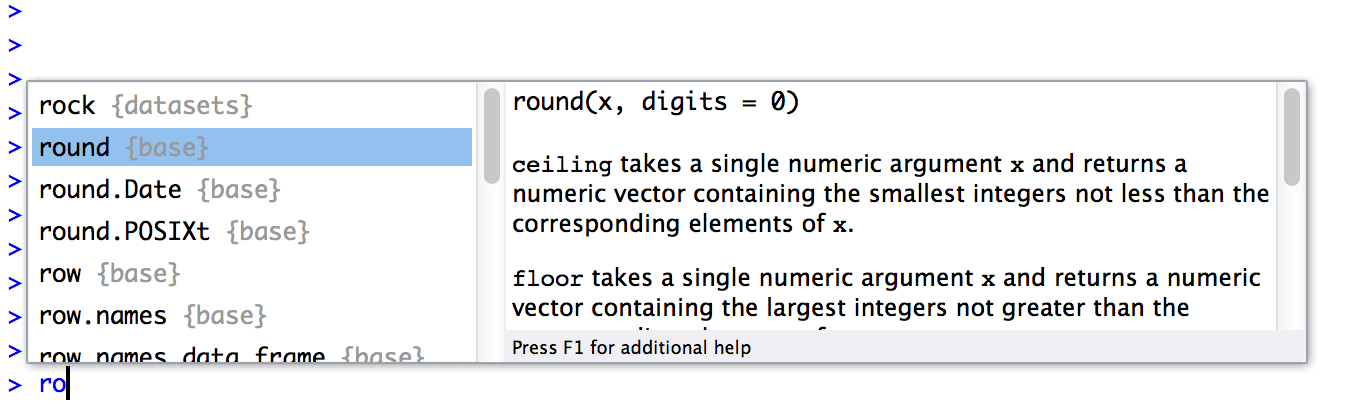
\includegraphics[width=18.94in]{./rbook-master/img/introR/RStudio_tab} \caption{Start typing the name of a function or a variable, and hit the "tab" key. RStudio brings up a little dialog box like this one that lets you select the one you want, and even prints out a little information about it.}\label{fig:RStudiotab}
\end{figure}

Start typing the name of a function or a variable, and hit the ``tab''
key. RStudio brings up a little dialog box like this one that lets you
select the one you want, and even prints out a little information about
it.

The RStudio autocomplete tool works slightly differently if you've
already got the name of the function typed and you're now trying to type
the arguments. For instance, suppose I've typed \texttt{round(} into the
console, and \emph{then} I hit tab. RStudio is smart enough to recognise
that I already know the name of the function that I want, because I've
already typed it! Instead, it figures that what I'm interested in is the
\emph{arguments} to that function. So that's what pops up in the little
window. You can see this in Figure \ref{fig:RStudiotab2}. Again, the
window has two panels, and you can interact with this window in exactly
the same way that you did with the window shown in \ref{fig:RStudiotab}.
On the left hand panel, you can see a list of the argument names. On the
right hand side, it displays some information about what the selected
argument does.

\begin{figure}
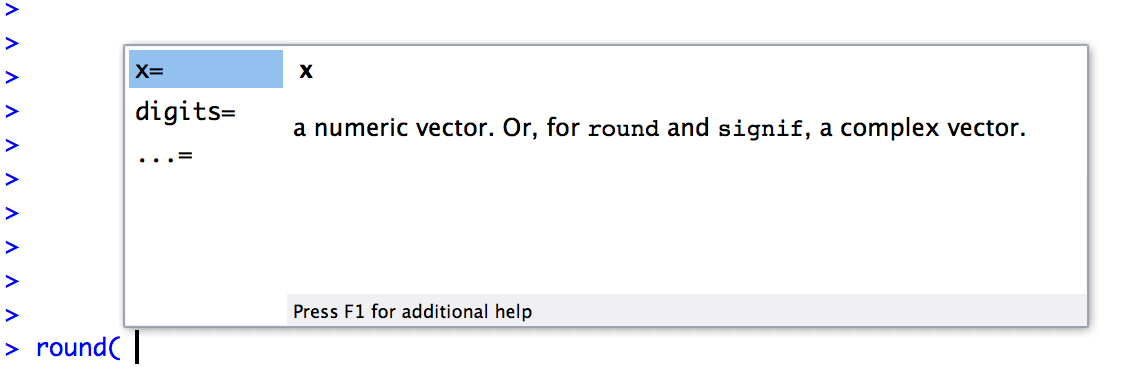
\includegraphics[width=15.82in]{./rbook-master/img/introR/RStudio_tab2} \caption{If you've typed the name of a function already along with the left parenthesis and then hit the "tab" key, RStudio brings up a different window to the one shown above. This one lists all the arguments to the function on the left, and information about each argument on the right.}\label{fig:unnamed-chunk-37}
\end{figure}

If you've typed the name of a function already along with the left
parenthesis and then hit the ``tab'' key, RStudio brings up a different
window to the one shown in Figure \ref{fig:RStudiotab}. This one lists
all the arguments to the function on the left, and information about
each argument on the right.

\subsection{Browsing your command
history}\label{browsing-your-command-history}

One thing that R does automatically is keep track of your ``command
history''. That is, it remembers all the commands that you've previously
typed. You can access this history in a few different ways. The simplest
way is to use the up and down arrow keys. If you hit the up key, the R
console will show you the most recent command that you've typed. Hit it
again, and it will show you the command before that. If you want the
text on the screen to go away, hit escape\footnote{Incidentally, that
  always works: if you've started typing a command and you want to clear
  it and start again, hit escape.} Using the up and down keys can be
really handy if you've typed a long command that had one typo in it.
Rather than having to type it all again from scratch, you can use the up
key to bring up the command and fix it.

The second way to get access to your command history is to look at the
history panel in RStudio. On the upper right hand side of the RStudio
window you'll see a tab labelled ``History''. Click on that, and you'll
see a list of all your recent commands displayed in that panel: it
should look something like Figure \ref{fig:RStudiohistory}. If you
double click on one of the commands, it will be copied to the R console.
(You can achieve the same result by selecting the command you want with
the mouse and then clicking the ``To Console'' button).\footnote{Another
  method is to start typing some text and then hit the Control key and
  the up arrow together (on Windows or Linux) or the Command key and the
  up arrow together (on a Mac). This will bring up a window showing all
  your recent commands that started with the same text as what you've
  currently typed. That can come in quite handy sometimes.}

\begin{figure}
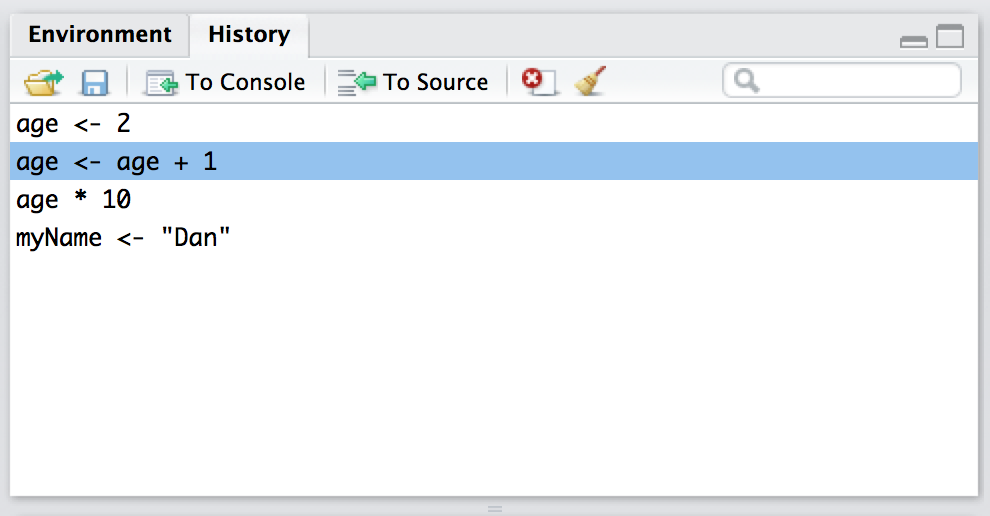
\includegraphics[width=13.75in]{./rbook-master/img/introR/historyTab} \caption{The history panel is located in the top right hand side of the RStudio window. Click on the word "History" and it displays this panel.}\label{fig:unnamed-chunk-38}
\end{figure}

\section{Storing many numbers as a vector}\label{vectors}

At this point we've covered functions in enough detail to get us safely
through the next couple of chapters (with one small exception: see
Section\ref{generics}, so let's return to our discussion of variables.
When I introduced variables in Section\ref{assign} I showed you how we
can use variables to store a single number. In this section, we'll
extend this idea and look at how to store multiple numbers within the
one variable. In R, the name for a variable that can store multiple
values is a \textbf{\emph{vector}}. So let's create one.

\subsection{Creating a vector}\label{creating-a-vector}

Let's stick to my silly ``get rich quick by textbook writing'' example.
Suppose the textbook company (if I actually had one, that is) sends me
sales data on a monthly basis. Since my class start in late February, we
might expect most of the sales to occur towards the start of the year.
Let's suppose that I have 100 sales in February, 200 sales in March and
50 sales in April, and no other sales for the rest of the year. What I
would like to do is have a variable -- let's call it
\texttt{sales.by.month} -- that stores all this sales data. The first
number stored should be \texttt{0} since I had no sales in January, the
second should be \texttt{100}, and so on. The simplest way to do this in
R is to use the \textbf{\emph{combine}} function, \texttt{c()}. To do
so, all we have to do is type all the numbers you want to store in a
comma separated list, like this:\footnote{Notice that I didn't specify
  any argument names here. The \texttt{c()} function is one of those
  cases where we don't use names. We just type all the numbers, and R
  just dumps them all in a single variable.}

\begin{Shaded}
\begin{Highlighting}[]
\NormalTok{sales.by.month <-}\StringTok{ }\KeywordTok{c}\NormalTok{(}\DecValTok{0}\NormalTok{, }\DecValTok{100}\NormalTok{, }\DecValTok{200}\NormalTok{, }\DecValTok{50}\NormalTok{, }\DecValTok{0}\NormalTok{, }\DecValTok{0}\NormalTok{, }\DecValTok{0}\NormalTok{, }\DecValTok{0}\NormalTok{, }\DecValTok{0}\NormalTok{, }\DecValTok{0}\NormalTok{, }\DecValTok{0}\NormalTok{, }\DecValTok{0}\NormalTok{)}
\NormalTok{sales.by.month}
\end{Highlighting}
\end{Shaded}

\begin{verbatim}
##  [1]   0 100 200  50   0   0   0   0   0   0   0   0
\end{verbatim}

To use the correct terminology here, we have a single variable here
called \texttt{sales.by.month}: this variable is a vector that consists
of 12 \textbf{\emph{elements}}.

\subsection{A handy digression}\label{a-handy-digression}

Now that we've learned how to put information into a vector, the next
thing to understand is how to pull that information back out again.
However, before I do so it's worth taking a slight detour. If you've
been following along, typing all the commands into R yourself, it's
possible that the output that you saw when we printed out the
\texttt{sales.by.month} vector was slightly different to what I showed
above. This would have happened if the window (or the RStudio panel)
that contains the R console is really, really narrow. If that were the
case, you might have seen output that looks something like this:

\begin{Shaded}
\begin{Highlighting}[]
\NormalTok{sales.by.month}
\end{Highlighting}
\end{Shaded}

\begin{verbatim}
##  [1]   0 100 200  50   0   0   0   0   0   0   0   0
\end{verbatim}

Because there wasn't much room on the screen, R has printed out the
results over two lines. But that's not the important thing to notice.
The important point is that the first line has a \texttt{{[}1{]}} in
front of it, whereas the second line starts with \texttt{{[}9{]}}. It's
pretty clear what's happening here. For the first row, R has printed out
the 1st element through to the 8th element, so it starts that row with a
\texttt{{[}1{]}}. For the second row, R has printed out the 9th element
of the vector through to the 12th one, and so it begins that row with a
\texttt{{[}9{]}} so that you can tell where it's up to at a glance. It
might seem a bit odd to you that R does this, but in some ways it's a
kindness, especially when dealing with larger data sets!

\subsection{Getting information out of vectors}\label{vectorsubset}

To get back to the main story, let's consider the problem of how to get
information out of a vector. At this point, you might have a sneaking
suspicion that the answer has something to do with the \texttt{{[}1{]}}
and \texttt{{[}9{]}} things that R has been printing out. And of course
you are correct. Suppose I want to pull out the February sales data
only. February is the second month of the year, so let's try this:

\begin{Shaded}
\begin{Highlighting}[]
\NormalTok{sales.by.month[}\DecValTok{2}\NormalTok{]}
\end{Highlighting}
\end{Shaded}

\begin{verbatim}
## [1] 100
\end{verbatim}

Yep, that's the February sales all right. But there's a subtle detail to
be aware of here: notice that R outputs \texttt{{[}1{]}\ 100},
\emph{not} \texttt{{[}2{]}\ 100}. This is because R is being extremely
literal. When we typed in \texttt{sales.by.month{[}2{]}}, we asked R to
find exactly \emph{one} thing, and that one thing happens to be the
second element of our \texttt{sales.by.month} vector. So, when it
outputs \texttt{{[}1{]}\ 100} what R is saying is that the first number
\emph{that we just asked for} is \texttt{100}. This behaviour makes more
sense when you realise that we can use this trick to create new
variables. For example, I could create a \texttt{february.sales}
variable like this:

\begin{Shaded}
\begin{Highlighting}[]
\NormalTok{february.sales <-}\StringTok{ }\NormalTok{sales.by.month[}\DecValTok{2}\NormalTok{]}
\NormalTok{february.sales}
\end{Highlighting}
\end{Shaded}

\begin{verbatim}
## [1] 100
\end{verbatim}

Obviously, the new variable \texttt{february.sales} should only have one
element and so when I print it out this new variable, the R output
begins with a \texttt{{[}1{]}} because \texttt{100} is the value of the
first (and only) element of \texttt{february.sales}. The fact that this
also happens to be the value of the second element of
\texttt{sales.by.month} is irrelevant. We'll pick this topic up again
shortly (Section\ref{indexing}.

\subsection{Altering the elements of a
vector}\label{altering-the-elements-of-a-vector}

Sometimes you'll want to change the values stored in a vector. Imagine
my surprise when the publisher rings me up to tell me that the sales
data for May are wrong. There were actually an additional 25 books sold
in May, but there was an error or something so they hadn't told me about
it. How can I fix my \texttt{sales.by.month} variable? One possibility
would be to assign the whole vector again from the beginning, using
\texttt{c()}. But that's a lot of typing. Also, it's a little wasteful:
why should R have to redefine the sales figures for all 12 months, when
only the 5th one is wrong? Fortunately, we can tell R to change only the
5th element, using this trick:

\begin{Shaded}
\begin{Highlighting}[]
\NormalTok{sales.by.month[}\DecValTok{5}\NormalTok{] <-}\StringTok{ }\DecValTok{25}
\NormalTok{sales.by.month}
\end{Highlighting}
\end{Shaded}

\begin{verbatim}
##  [1]   0 100 200  50  25   0   0   0   0   0   0   0
\end{verbatim}

Another way to edit variables is to use the \texttt{edit()} or
\texttt{fix()} functions. I won't discuss them in detail right now, but
you can check them out on your own.

\subsection{Useful things to know about vectors}\label{veclength}

Before moving on, I want to mention a couple of other things about
vectors. Firstly, you often find yourself wanting to know how many
elements there are in a vector (usually because you've forgotten). You
can use the \texttt{length()} function to do this. It's quite
straightforward:

\begin{Shaded}
\begin{Highlighting}[]
\KeywordTok{length}\NormalTok{( }\DataTypeTok{x =}\NormalTok{ sales.by.month )}
\end{Highlighting}
\end{Shaded}

\begin{verbatim}
## [1] 12
\end{verbatim}

Secondly, you often want to alter all of the elements of a vector at
once. For instance, suppose I wanted to figure out how much money I made
in each month. Since I'm earning an exciting \$7 per book (no seriously,
that's actually pretty close to what authors get on the very expensive
textbooks that you're expected to purchase), what I want to do is
multiply each element in the \texttt{sales.by.month} vector by
\texttt{7}. R makes this pretty easy, as the following example shows:

\begin{Shaded}
\begin{Highlighting}[]
\NormalTok{sales.by.month }\OperatorTok{*}\StringTok{ }\DecValTok{7}
\end{Highlighting}
\end{Shaded}

\begin{verbatim}
##  [1]    0  700 1400  350  175    0    0    0    0    0    0    0
\end{verbatim}

In other words, when you multiply a vector by a single number, all
elements in the vector get multiplied. The same is true for addition,
subtraction, division and taking powers. So that's neat. On the other
hand, suppose I wanted to know how much money I was making per day,
rather than per month. Since not every month has the same number of
days, I need to do something slightly different. Firstly, I'll create
two new vectors:

\begin{Shaded}
\begin{Highlighting}[]
\NormalTok{days.per.month <-}\StringTok{ }\KeywordTok{c}\NormalTok{(}\DecValTok{31}\NormalTok{, }\DecValTok{28}\NormalTok{, }\DecValTok{31}\NormalTok{, }\DecValTok{30}\NormalTok{, }\DecValTok{31}\NormalTok{, }\DecValTok{30}\NormalTok{, }\DecValTok{31}\NormalTok{, }\DecValTok{31}\NormalTok{, }\DecValTok{30}\NormalTok{, }\DecValTok{31}\NormalTok{, }\DecValTok{30}\NormalTok{, }\DecValTok{31}\NormalTok{)}
\NormalTok{profit <-}\StringTok{ }\NormalTok{sales.by.month }\OperatorTok{*}\StringTok{ }\DecValTok{7}
\end{Highlighting}
\end{Shaded}

Obviously, the \texttt{profit} variable is the same one we created
earlier, and the \texttt{days.per.month} variable is pretty
straightforward. What I want to do is divide every element of
\texttt{profit} by the \emph{corresponding} element of
\texttt{days.per.month}. Again, R makes this pretty easy:

\begin{Shaded}
\begin{Highlighting}[]
\NormalTok{profit }\OperatorTok{/}\StringTok{ }\NormalTok{days.per.month}
\end{Highlighting}
\end{Shaded}

\begin{verbatim}
##  [1]  0.000000 25.000000 45.161290 11.666667  5.645161  0.000000  0.000000
##  [8]  0.000000  0.000000  0.000000  0.000000  0.000000
\end{verbatim}

I still don't like all those zeros, but that's not what matters here.
Notice that the second element of the output is 25, because R has
divided the second element of \texttt{profit} (i.e.~700) by the second
element of \texttt{days.per.month} (i.e.~28). Similarly, the third
element of the output is equal to 1400 divided by 31, and so on. We'll
talk more about calculations involving vectors later on (and in
particular a thing called the ``recycling rule''; Section
\ref{recycling}, but that's enough detail for now.

\section{Storing text data}\label{text}

A lot of the time your data will be numeric in nature, but not always.
Sometimes your data really needs to be described using text, not using
numbers. To address this, we need to consider the situation where our
variables store text. To create a variable that stores the word
``hello'', we can type this:

\begin{Shaded}
\begin{Highlighting}[]
\NormalTok{greeting <-}\StringTok{ "hello"}
\NormalTok{greeting}
\end{Highlighting}
\end{Shaded}

\begin{verbatim}
## [1] "hello"
\end{verbatim}

When interpreting this, it's important to recognise that the quote marks
here \emph{aren't} part of the string itself. They're just something
that we use to make sure that R knows to treat the characters that they
enclose as a piece of text data, known as a \textbf{\emph{character
string}}. In other words, R treats \texttt{"hello"} as a string
containing the word ``hello''; but if I had typed \texttt{hello}
instead, R would go looking for a variable by that name! You can also
use \texttt{\textquotesingle{}hello\textquotesingle{}} to specify a
character string.

Okay, so that's how we store the text. Next, it's important to recognise
that when we do this, R stores the entire word \texttt{"hello"} as a
\emph{single} element: our \texttt{greeting} variable is \emph{not} a
vector of five different letters. Rather, it has only the one element,
and that element corresponds to the entire character string
\texttt{"hello"}. To illustrate this, if I actually ask R to find the
first element of \texttt{greeting}, it prints the whole string:

\begin{Shaded}
\begin{Highlighting}[]
\NormalTok{greeting[}\DecValTok{1}\NormalTok{]}
\end{Highlighting}
\end{Shaded}

\begin{verbatim}
## [1] "hello"
\end{verbatim}

Of course, there's no reason why I can't create a vector of character
strings. For instance, if we were to continue with the example of my
attempts to look at the monthly sales data for my book, one variable I
might want would include the names of all 12
\texttt{months}.\^{}{[}Though actually there's no real need to do this,
since R has an inbuilt variable called
\texttt{month.name{]}\ that\ you\ can\ use\ for\ this\ purpose.} To do
so, I could type in a command like this

\begin{Shaded}
\begin{Highlighting}[]
\NormalTok{months <-}\StringTok{ }\KeywordTok{c}\NormalTok{(}\StringTok{"January"}\NormalTok{, }\StringTok{"February"}\NormalTok{, }\StringTok{"March"}\NormalTok{, }\StringTok{"April"}\NormalTok{, }\StringTok{"May"}\NormalTok{, }\StringTok{"June"}\NormalTok{,}
            \StringTok{"July"}\NormalTok{, }\StringTok{"August"}\NormalTok{, }\StringTok{"September"}\NormalTok{, }\StringTok{"October"}\NormalTok{, }\StringTok{"November"}\NormalTok{, }
            \StringTok{"December"}\NormalTok{)}
\end{Highlighting}
\end{Shaded}

This is a \textbf{\emph{character vector}} containing 12 elements, each
of which is the name of a month. So if I wanted R to tell me the name of
the fourth month, all I would do is this:

\begin{Shaded}
\begin{Highlighting}[]
\NormalTok{months[}\DecValTok{4}\NormalTok{]}
\end{Highlighting}
\end{Shaded}

\begin{verbatim}
## [1] "April"
\end{verbatim}

\subsection{Working with text}\label{simpletext}

Working with text data is somewhat more complicated than working with
numeric data, and I discuss some of the basic ideas in Section
\ref{textprocessing}, but for purposes of the current chapter we only
need this bare bones sketch. The only other thing I want to do before
moving on is show you an example of a function that can be applied to
text data. So far, most of the functions that we have seen (i.e.,
\texttt{sqrt()}, \texttt{abs()} and \texttt{round()}) only make sense
when applied to numeric data (e.g., you can't calculate the square root
of ``hello''), and we've seen one function that can be applied to pretty
much any variable or vector (i.e., \texttt{length()}). So it might be
nice to see an example of a function that can be applied to text.

The function I'm going to introduce you to is called \texttt{nchar()},
and what it does is count the number of individual characters that make
up a string. Recall earlier that when we tried to calculate the
\texttt{length()} of our \texttt{greeting} variable it returned a value
of \texttt{1}: the \texttt{greeting} variable contains only the one
string, which happens to be \texttt{"hello"}. But what if I want to know
how many letters there are in the word? Sure, I could \emph{count} them,
but that's boring, and more to the point it's a terrible strategy if
what I wanted to know was the number of letters in \emph{War and Peace}.
That's where the \texttt{nchar()} function is helpful:

\begin{Shaded}
\begin{Highlighting}[]
\KeywordTok{nchar}\NormalTok{( }\DataTypeTok{x =}\NormalTok{ greeting )}
\end{Highlighting}
\end{Shaded}

\begin{verbatim}
## [1] 5
\end{verbatim}

That makes sense, since there are in fact 5 letters in the string
\texttt{"hello"}. Better yet, you can apply \texttt{nchar()} to whole
vectors. So, for instance, if I want R to tell me how many letters there
are in the names of each of the 12 months, I can do this:

\begin{Shaded}
\begin{Highlighting}[]
\KeywordTok{nchar}\NormalTok{( }\DataTypeTok{x =}\NormalTok{ months )}
\end{Highlighting}
\end{Shaded}

\begin{verbatim}
##  [1] 7 8 5 5 3 4 4 6 9 7 8 8
\end{verbatim}

So that's nice to know. The \texttt{nchar()} function can do a bit more
than this, and there's a lot of other functions that you can do to
extract more information from text or do all sorts of fancy things.
However, the goal here is not to teach any of that! The goal right now
is just to see an example of a function that actually does work when
applied to text.

\section{\texorpdfstring{Storing ``true or false''
data}{Storing true or false data}}\label{logicals}

Time to move onto a third kind of data. A key concept in that a lot of R
relies on is the idea of a \textbf{\emph{logical value}}. A logical
value is an assertion about whether something is true or false. This is
implemented in R in a pretty straightforward way. There are two logical
values, namely \texttt{TRUE} and \texttt{FALSE}. Despite the simplicity,
a logical values are very useful things. Let's see how they work.

\subsection{Assessing mathematical
truths}\label{assessing-mathematical-truths}

In George Orwell's classic book \emph{1984}, one of the slogans used by
the totalitarian Party was ``two plus two equals five'', the idea being
that the political domination of human freedom becomes complete when it
is possible to subvert even the most basic of truths. It's a terrifying
thought, especially when the protagonist Winston Smith finally breaks
down under torture and agrees to the proposition. ``Man is infinitely
malleable'', the book says. I'm pretty sure that this isn't true of
humans\footnote{I offer up my teenage attempts to be ``cool'' as
  evidence that some things just can't be done.} but it's definitely not
true of R. R is not infinitely malleable. It has rather firm opinions on
the topic of what is and isn't true, at least as regards basic
mathematics. If I ask it to calculate \texttt{2\ +\ 2}, it always gives
the same answer, and it's not bloody 5:

\begin{Shaded}
\begin{Highlighting}[]
\DecValTok{2} \OperatorTok{+}\StringTok{ }\DecValTok{2}
\end{Highlighting}
\end{Shaded}

\begin{verbatim}
## [1] 4
\end{verbatim}

Of course, so far R is just doing the calculations. I haven't asked it
to explicitly assert that \(2+2 = 4\) is a true statement. If I want R
to make an explicit judgement, I can use a command like this:

\begin{Shaded}
\begin{Highlighting}[]
\DecValTok{2} \OperatorTok{+}\StringTok{ }\DecValTok{2} \OperatorTok{==}\StringTok{ }\DecValTok{4}
\end{Highlighting}
\end{Shaded}

\begin{verbatim}
## [1] TRUE
\end{verbatim}

What I've done here is use the \textbf{\emph{equality operator}},
\texttt{==}, to force R to make a ``true or false'' judgement.\footnote{Note
  that this is a very different operator to the assignment operator
  \texttt{=} that I talked about in Section\ref{assign}. A common typo
  that people make when trying to write logical commands in R (or other
  languages, since the ``\texttt{=} versus \texttt{==}'' distinction is
  important in most programming languages) is to accidentally type
  \texttt{=} when you really mean \texttt{==}. Be especially cautious
  with this -- I've been programming in various languages since I was a
  teenager, and I \emph{still} screw this up a lot. Hm. I think I see
  why I wasn't cool as a teenager. And why I'm still not cool.} Okay,
let's see what R thinks of the Party slogan:

\begin{Shaded}
\begin{Highlighting}[]
\DecValTok{2}\OperatorTok{+}\DecValTok{2} \OperatorTok{==}\StringTok{ }\DecValTok{5}
\end{Highlighting}
\end{Shaded}

\begin{verbatim}
## [1] FALSE
\end{verbatim}

Booyah! Freedom and ponies for all! Or something like that. Anyway, it's
worth having a look at what happens if I try to \emph{force} R to
believe that two plus two is five by making an assignment statement like
\texttt{2\ +\ 2\ =\ 5} or \texttt{2\ +\ 2\ \textless{}-\ 5}. When I do
this, here's what happens:

\begin{Shaded}
\begin{Highlighting}[]
\DecValTok{2} \OperatorTok{+}\StringTok{ }\DecValTok{2}\NormalTok{ =}\StringTok{ }\DecValTok{5}
\end{Highlighting}
\end{Shaded}

\begin{verbatim}
## Error in 2 + 2 = 5: target of assignment expands to non-language object
\end{verbatim}

R doesn't like this very much. It recognises that \texttt{2\ +\ 2} is
\emph{not} a variable (that's what the ``non-language object'' part is
saying), and it won't let you try to ``reassign'' it. While R is pretty
flexible, and actually does let you do some quite remarkable things to
redefine parts of R itself, there are just some basic, primitive truths
that it refuses to give up. It won't change the laws of addition, and it
won't change the definition of the number \texttt{2}.

That's probably for the best.

\hypertarget{logical-operations}{\subsection{Logical
operations}\label{logical-operations}}

So now we've seen logical operations at work, but so far we've only seen
the simplest possible example. You probably won't be surprised to
discover that we can combine logical operations with other operations
and functions in a more complicated way, like this:

\begin{Shaded}
\begin{Highlighting}[]
\DecValTok{3}\OperatorTok{*}\DecValTok{3} \OperatorTok{+}\StringTok{ }\DecValTok{4}\OperatorTok{*}\DecValTok{4} \OperatorTok{==}\StringTok{ }\DecValTok{5}\OperatorTok{*}\DecValTok{5}
\end{Highlighting}
\end{Shaded}

\begin{verbatim}
## [1] TRUE
\end{verbatim}

or this

\begin{Shaded}
\begin{Highlighting}[]
\KeywordTok{sqrt}\NormalTok{( }\DecValTok{25}\NormalTok{ ) }\OperatorTok{==}\StringTok{ }\DecValTok{5}
\end{Highlighting}
\end{Shaded}

\begin{verbatim}
## [1] TRUE
\end{verbatim}

Not only that, but as Table \ref{tab:logicals} illustrates, there are
several other logical operators that you can use, corresponding to some
basic mathematical concepts.

\begin{table}

\caption{\label{tab:logicals}Some logical operators. Technically I should be calling these "binary relational operators", but quite frankly I don't want to. It's my book so no-one can make me.}
\centering
\begin{tabular}[t]{llll}
\toprule
operation & operator & example input & answer\\
\midrule
less than & < & 2 < 3 & `TRUE`\\
less than or equal to & <= & 2 <= 2 & `TRUE`\\
greater than & > & 2 > 3 & `FALSE`\\
greater than or equal to & >= & 2 >= 2 & `TRUE`\\
equal to & == & 2 == 3 & `FALSE`\\
not equal to & != & 2 != 3 & `TRUE`\\
\bottomrule
\end{tabular}
\end{table}

Hopefully these are all pretty self-explanatory: for example, the
\textbf{\emph{less than}} operator \texttt{\textless{}} checks to see if
the number on the left is less than the number on the right. If it's
less, then R returns an answer of \texttt{TRUE}:

\begin{Shaded}
\begin{Highlighting}[]
\DecValTok{99} \OperatorTok{<}\StringTok{ }\DecValTok{100}
\end{Highlighting}
\end{Shaded}

\begin{verbatim}
## [1] TRUE
\end{verbatim}

but if the two numbers are equal, or if the one on the right is larger,
then R returns an answer of \texttt{FALSE}, as the following two
examples illustrate:

\begin{Shaded}
\begin{Highlighting}[]
\DecValTok{100} \OperatorTok{<}\StringTok{ }\DecValTok{100}
\end{Highlighting}
\end{Shaded}

\begin{verbatim}
## [1] FALSE
\end{verbatim}

\begin{Shaded}
\begin{Highlighting}[]
\DecValTok{100} \OperatorTok{<}\StringTok{ }\DecValTok{99}
\end{Highlighting}
\end{Shaded}

\begin{verbatim}
## [1] FALSE
\end{verbatim}

In contrast, the \textbf{\emph{less than or equal to}} operator
\texttt{\textless{}=} will do exactly what it says. It returns a value
of \texttt{TRUE} if the number of the left hand side is less than or
equal to the number on the right hand side. So if we repeat the previous
two examples using \texttt{\textless{}=}, here's what we get:

\begin{Shaded}
\begin{Highlighting}[]
\DecValTok{100} \OperatorTok{<=}\StringTok{ }\DecValTok{100}
\end{Highlighting}
\end{Shaded}

\begin{verbatim}
## [1] TRUE
\end{verbatim}

\begin{Shaded}
\begin{Highlighting}[]
\DecValTok{100} \OperatorTok{<=}\StringTok{ }\DecValTok{99}
\end{Highlighting}
\end{Shaded}

\begin{verbatim}
## [1] FALSE
\end{verbatim}

And at this point I hope it's pretty obvious what the
\textbf{\emph{greater than}} operator \texttt{\textgreater{}} and the
\textbf{\emph{greater than or equal to}} operator
\texttt{\textgreater{}=} do! Next on the list of logical operators is
the \textbf{\emph{not equal to}} operator \texttt{!=} which -- as with
all the others -- does what it says it does. It returns a value of
\texttt{TRUE} when things on either side are not identical to each
other. Therefore, since \(2+2\) isn't equal to \(5\), we get:

\begin{Shaded}
\begin{Highlighting}[]
\DecValTok{2} \OperatorTok{+}\StringTok{ }\DecValTok{2} \OperatorTok{!=}\StringTok{ }\DecValTok{5}
\end{Highlighting}
\end{Shaded}

\begin{verbatim}
## [1] TRUE
\end{verbatim}

We're not quite done yet. There are three more logical operations that
are worth knowing about, listed in Table \ref{tab:logicals2}.

\begin{table}

\caption{\label{tab:logicals2}Some more logical operators.}
\centering
\begin{tabular}[t]{llll}
\toprule
operation & operator & example input & answer\\
\midrule
not & ! & !(1==1) & `FALSE`\\
or & | & (1==1) | (2==3) & `TRUE`\\
and & \& & (1==1) \& (2==3) & `FALSE`\\
\bottomrule
\end{tabular}
\end{table}

These are the \textbf{\emph{not}} operator \texttt{!}, the
\textbf{\emph{and}} operator \texttt{\&}, and the \textbf{\emph{or}}
operator \texttt{\textbar{}}. Like the other logical operators, their
behaviour is more or less exactly what you'd expect given their names.
For instance, if I ask you to assess the claim that ``either \(2+2 = 4\)
\emph{or} \(2+2 = 5\)'' you'd say that it's true. Since it's an
``either-or'' statement, all we need is for one of the two parts to be
true. That's what the \texttt{\textbar{}} operator does:

\begin{Shaded}
\begin{Highlighting}[]
\NormalTok{(}\DecValTok{2}\OperatorTok{+}\DecValTok{2} \OperatorTok{==}\StringTok{ }\DecValTok{4}\NormalTok{) }\OperatorTok{|}\StringTok{ }\NormalTok{(}\DecValTok{2}\OperatorTok{+}\DecValTok{2} \OperatorTok{==}\StringTok{ }\DecValTok{5}\NormalTok{)}
\end{Highlighting}
\end{Shaded}

\begin{verbatim}
## [1] TRUE
\end{verbatim}

On the other hand, if I ask you to assess the claim that ``both
\(2+2 = 4\) \emph{and} \(2+2 = 5\)'' you'd say that it's false. Since
this is an \emph{and} statement we need both parts to be true. And
that's what the \texttt{\&} operator does:

\begin{Shaded}
\begin{Highlighting}[]
\NormalTok{(}\DecValTok{2}\OperatorTok{+}\DecValTok{2} \OperatorTok{==}\StringTok{ }\DecValTok{4}\NormalTok{) }\OperatorTok{&}\StringTok{ }\NormalTok{(}\DecValTok{2}\OperatorTok{+}\DecValTok{2} \OperatorTok{==}\StringTok{ }\DecValTok{5}\NormalTok{)}
\end{Highlighting}
\end{Shaded}

\begin{verbatim}
## [1] FALSE
\end{verbatim}

Finally, there's the \emph{not} operator, which is simple but annoying
to describe in English. If I ask you to assess my claim that ``it is not
true that \(2+2 = 5\)'' then you would say that my claim is true;
because my claim is that ``\(2+2 = 5\) is false''. And I'm right. If we
write this as an R command we get this:

\begin{Shaded}
\begin{Highlighting}[]
\OperatorTok{!}\StringTok{ }\NormalTok{(}\DecValTok{2}\OperatorTok{+}\DecValTok{2} \OperatorTok{==}\StringTok{ }\DecValTok{5}\NormalTok{)}
\end{Highlighting}
\end{Shaded}

\begin{verbatim}
## [1] TRUE
\end{verbatim}

In other words, since \texttt{2+2\ ==\ 5} is a \texttt{FALSE} statement,
it must be the case that \texttt{!(2+2\ ==\ 5)} is a \texttt{TRUE} one.
Essentially, what we've really done is claim that ``not false'' is the
same thing as ``true''. Obviously, this isn't really quite right in real
life. But R lives in a much more black or white world: for R everything
is either true or false. No shades of gray are allowed. We can actually
see this much more explicitly, like this:

\begin{Shaded}
\begin{Highlighting}[]
\OperatorTok{!}\StringTok{ }\OtherTok{FALSE}
\end{Highlighting}
\end{Shaded}

\begin{verbatim}
## [1] TRUE
\end{verbatim}

Of course, in our \(2+2 = 5\) example, we didn't really need to use
``not'' \texttt{!} and ``equals to'' \texttt{==} as two separate
operators. We could have just used the ``not equals to'' operator
\texttt{!=} like this:

\begin{Shaded}
\begin{Highlighting}[]
\DecValTok{2}\OperatorTok{+}\DecValTok{2} \OperatorTok{!=}\StringTok{ }\DecValTok{5}
\end{Highlighting}
\end{Shaded}

\begin{verbatim}
## [1] TRUE
\end{verbatim}

But there are many situations where you really do need to use the
\texttt{!} operator. We'll see some later on.\footnote{A note for those
  of you who have taken a computer science class: yes, R does have a
  function for exclusive-or, namely \texttt{xor()}. Also worth noting is
  the fact that R makes the distinction between element-wise operators
  \texttt{\&} and \texttt{\textbar{}} and operators that look only at
  the first element of the vector, namely \texttt{\&\&} and
  \texttt{\textbar{}\textbar{}}. To see the distinction, compare the
  behaviour of a command like \texttt{c(FALSE,TRUE)\ \&\ c(TRUE,TRUE)}
  to the behaviour of something like
  \texttt{c(FALSE,TRUE)\ \&\&\ c(TRUE,TRUE)}. If this doesn't mean
  anything to you, ignore this footnote entirely. It's not important for
  the content of this book.}

\subsection{Storing and using logical
data}\label{storing-and-using-logical-data}

Up to this point, I've introduced \emph{numeric data} (in Sections
\ref{assign} and @ref(\#vectors)) and \emph{character data} (in Section
\ref{text}). So you might not be surprised to discover that these
\texttt{TRUE} and \texttt{FALSE} values that R has been producing are
actually a third kind of data, called \emph{logical data}. That is, when
I asked R if \texttt{2\ +\ 2\ ==\ 5} and it said \texttt{{[}1{]}\ FALSE}
in reply, it was actually producing information that we can store in
variables. For instance, I could create a variable called
\texttt{is.the.Party.correct}, which would store R's opinion:

\begin{Shaded}
\begin{Highlighting}[]
\NormalTok{is.the.Party.correct <-}\StringTok{ }\DecValTok{2} \OperatorTok{+}\StringTok{ }\DecValTok{2} \OperatorTok{==}\StringTok{ }\DecValTok{5}
\NormalTok{is.the.Party.correct}
\end{Highlighting}
\end{Shaded}

\begin{verbatim}
## [1] FALSE
\end{verbatim}

Alternatively, you can assign the value directly, by typing
\texttt{TRUE} or \texttt{FALSE} in your command. Like this:

\begin{Shaded}
\begin{Highlighting}[]
\NormalTok{is.the.Party.correct <-}\StringTok{ }\OtherTok{FALSE}
\NormalTok{is.the.Party.correct}
\end{Highlighting}
\end{Shaded}

\begin{verbatim}
## [1] FALSE
\end{verbatim}

Better yet, because it's kind of tedious to type \texttt{TRUE} or
\texttt{FALSE} over and over again, R provides you with a shortcut: you
can use \texttt{T} and \texttt{F} instead (but it's case sensitive:
\texttt{t} and \texttt{f} won't work).\footnote{Warning! \texttt{TRUE}
  and \texttt{FALSE} are reserved keywords in R, so you can trust that
  they always mean what they say they do. Unfortunately, the shortcut
  versions \texttt{T} and \texttt{F} do not have this property. It's
  even possible to create variables that set up the reverse meanings, by
  typing commands like \texttt{T\ \textless{}-\ FALSE} and
  \texttt{F\ \textless{}-\ TRUE}. This is kind of insane, and something
  that is generally thought to be a design flaw in R. Anyway, the long
  and short of it is that it's safer to use \texttt{TRUE} and
  \texttt{FALSE}.}So this works:

\begin{Shaded}
\begin{Highlighting}[]
\NormalTok{is.the.Party.correct <-}\StringTok{ }\NormalTok{F}
\NormalTok{is.the.Party.correct}
\end{Highlighting}
\end{Shaded}

\begin{verbatim}
## [1] FALSE
\end{verbatim}

but this doesn't:

\begin{Shaded}
\begin{Highlighting}[]
\NormalTok{is.the.Party.correct <-}\StringTok{ }\NormalTok{f}
\end{Highlighting}
\end{Shaded}

\begin{verbatim}
## Error in eval(expr, envir, enclos): object 'f' not found
\end{verbatim}

\subsection{Vectors of logicals}\label{vectors-of-logicals}

The next thing to mention is that you can store vectors of logical
values in exactly the same way that you can store vectors of numbers
(Section\ref{vectors}) and vectors of text data (Section\ref{text}).
Again, we can define them directly via the \texttt{c()} function, like
this:

\begin{Shaded}
\begin{Highlighting}[]
\NormalTok{x <-}\StringTok{ }\KeywordTok{c}\NormalTok{(}\OtherTok{TRUE}\NormalTok{, }\OtherTok{TRUE}\NormalTok{, }\OtherTok{FALSE}\NormalTok{)}
\NormalTok{x}
\end{Highlighting}
\end{Shaded}

\begin{verbatim}
## [1]  TRUE  TRUE FALSE
\end{verbatim}

or you can produce a vector of logicals by applying a logical operator
to a vector. This might not make a lot of sense to you, so let's unpack
it slowly. First, let's suppose we have a vector of numbers (i.e., a
``non-logical vector''). For instance, we could use the
\texttt{sales.by.month} vector that we were using in
Section@ref(\#vectors). Suppose I wanted R to tell me, for each month of
the year, whether I actually sold a book in that month. I can do that by
typing this:

\begin{Shaded}
\begin{Highlighting}[]
\NormalTok{sales.by.month }\OperatorTok{>}\StringTok{ }\DecValTok{0}
\end{Highlighting}
\end{Shaded}

\begin{verbatim}
##  [1] FALSE  TRUE  TRUE  TRUE  TRUE FALSE FALSE FALSE FALSE FALSE FALSE
## [12] FALSE
\end{verbatim}

and again, I can store this in a vector if I want, as the example below
illustrates:

\begin{Shaded}
\begin{Highlighting}[]
\NormalTok{any.sales.this.month <-}\StringTok{ }\NormalTok{sales.by.month }\OperatorTok{>}\StringTok{ }\DecValTok{0}
\NormalTok{any.sales.this.month}
\end{Highlighting}
\end{Shaded}

\begin{verbatim}
##  [1] FALSE  TRUE  TRUE  TRUE  TRUE FALSE FALSE FALSE FALSE FALSE FALSE
## [12] FALSE
\end{verbatim}

In other words, \texttt{any.sales.this.month} is a logical vector whose
elements are \texttt{TRUE} only if the corresponding element of
\texttt{sales.by.month} is greater than zero. For instance, since I sold
zero books in January, the first element is \texttt{FALSE}.

\subsection{Applying logical operation to text}\label{logictext}

In a moment (Section \ref{indexing}) I'll show you why these logical
operations and logical vectors are so handy, but before I do so I want
to very briefly point out that you can apply them to text as well as to
logical data. It's just that we need to be a bit more careful in
understanding how R interprets the different operations. In this section
I'll talk about how the equal to operator \texttt{==} applies to text,
since this is the most important one. Obviously, the not equal to
operator \texttt{!=} gives the exact opposite answers to \texttt{==} so
I'm implicitly talking about that one too, but I won't give specific
commands showing the use of \texttt{!=}. As for the other operators,
I'll defer a more detailed discussion of this topic to Section
\ref{logictext2}.

Okay, let's see how it works. In one sense, it's very simple. For
instance, I can ask R if the word \texttt{"cat"} is the same as the word
\texttt{"dog"}, like this:

\begin{Shaded}
\begin{Highlighting}[]
\StringTok{"cat"} \OperatorTok{==}\StringTok{ "dog"}
\end{Highlighting}
\end{Shaded}

\begin{verbatim}
## [1] FALSE
\end{verbatim}

That's pretty obvious, and it's good to know that even R can figure that
out. Similarly, R does recognise that a \texttt{"cat"} is a
\texttt{"cat"}:

\begin{Shaded}
\begin{Highlighting}[]
\StringTok{"cat"} \OperatorTok{==}\StringTok{ "cat"}
\end{Highlighting}
\end{Shaded}

\begin{verbatim}
## [1] TRUE
\end{verbatim}

Again, that's exactly what we'd expect. However, what you need to keep
in mind is that R is not at all tolerant when it comes to grammar and
spacing. If two strings differ in any way whatsoever, R will say that
they're not equal to each other, as the following examples indicate:

\begin{Shaded}
\begin{Highlighting}[]
\StringTok{" cat"} \OperatorTok{==}\StringTok{ "cat"}
\end{Highlighting}
\end{Shaded}

\begin{verbatim}
## [1] FALSE
\end{verbatim}

\begin{Shaded}
\begin{Highlighting}[]
\StringTok{"cat"} \OperatorTok{==}\StringTok{ "CAT"}
\end{Highlighting}
\end{Shaded}

\begin{verbatim}
## [1] FALSE
\end{verbatim}

\begin{Shaded}
\begin{Highlighting}[]
\StringTok{"cat"} \OperatorTok{==}\StringTok{ "c a t"}
\end{Highlighting}
\end{Shaded}

\begin{verbatim}
## [1] FALSE
\end{verbatim}

\section{Indexing vectors}\label{indexing}

One last thing to add before finishing up this chapter. So far, whenever
I've had to get information out of a vector, all I've done is typed
something like \texttt{months{[}4{]}}; and when I do this R prints out
the fourth element of the \texttt{months} vector. In this section, I'll
show you two additional tricks for getting information out of the
vector.

\subsection{Extracting multiple
elements}\label{extracting-multiple-elements}

One very useful thing we can do is pull out more than one element at a
time. In the previous example, we only used a single number (i.e.,
\texttt{2}) to indicate which element we wanted. Alternatively, we can
use a vector. So, suppose I wanted the data for February, March and
April. What I could do is use the vector \texttt{c(2,3,4)} to indicate
which elements I want R to pull out. That is, I'd type this:

\begin{Shaded}
\begin{Highlighting}[]
\NormalTok{sales.by.month[ }\KeywordTok{c}\NormalTok{(}\DecValTok{2}\NormalTok{,}\DecValTok{3}\NormalTok{,}\DecValTok{4}\NormalTok{) ]}
\end{Highlighting}
\end{Shaded}

\begin{verbatim}
## [1] 100 200  50
\end{verbatim}

Notice that the order matters here. If I asked for the data in the
reverse order (i.e., April first, then March, then February) by using
the vector \texttt{c(4,3,2)}, then R outputs the data in the reverse
order:

\begin{Shaded}
\begin{Highlighting}[]
\NormalTok{sales.by.month[ }\KeywordTok{c}\NormalTok{(}\DecValTok{4}\NormalTok{,}\DecValTok{3}\NormalTok{,}\DecValTok{2}\NormalTok{) ]}
\end{Highlighting}
\end{Shaded}

\begin{verbatim}
## [1]  50 200 100
\end{verbatim}

A second thing to be aware of is that R provides you with handy
shortcuts for very common situations. For instance, suppose that I
wanted to extract everything from the 2nd month through to the 8th
month. One way to do this is to do the same thing I did above, and use
the vector \texttt{c(2,3,4,5,6,7,8)} to indicate the elements that I
want. That works just fine

\begin{Shaded}
\begin{Highlighting}[]
\NormalTok{sales.by.month[ }\KeywordTok{c}\NormalTok{(}\DecValTok{2}\NormalTok{,}\DecValTok{3}\NormalTok{,}\DecValTok{4}\NormalTok{,}\DecValTok{5}\NormalTok{,}\DecValTok{6}\NormalTok{,}\DecValTok{7}\NormalTok{,}\DecValTok{8}\NormalTok{) ]}
\end{Highlighting}
\end{Shaded}

\begin{verbatim}
## [1] 100 200  50  25   0   0   0
\end{verbatim}

but it's kind of a lot of typing. To help make this easier, R lets you
use \texttt{2:8} as shorthand for \texttt{c(2,3,4,5,6,7,8)}, which makes
things a lot simpler. First, let's just check that this is true:

\begin{Shaded}
\begin{Highlighting}[]
\DecValTok{2}\OperatorTok{:}\DecValTok{8}
\end{Highlighting}
\end{Shaded}

\begin{verbatim}
## [1] 2 3 4 5 6 7 8
\end{verbatim}

Next, let's check that we can use the \texttt{2:8} shorthand as a way to
pull out the 2nd through 8th elements of \texttt{sales.by.months}:

\begin{Shaded}
\begin{Highlighting}[]
\NormalTok{sales.by.month[}\DecValTok{2}\OperatorTok{:}\DecValTok{8}\NormalTok{]}
\end{Highlighting}
\end{Shaded}

\begin{verbatim}
## [1] 100 200  50  25   0   0   0
\end{verbatim}

So that's kind of neat.

\subsection{Logical indexing}\label{logical-indexing}

At this point, I can introduce an extremely useful tool called
\textbf{\emph{logical indexing}}. In the last section, I created a
logical vector \texttt{any.sales.this.month}, whose elements are
\texttt{TRUE} for any month in which I sold at least one book, and
\texttt{FALSE} for all the others. However, that big long list of
\texttt{TRUE}s and \texttt{FALSE}s is a little bit hard to read, so what
I'd like to do is to have R select the names of the \texttt{months} for
which I sold any books. Earlier on, I created a vector \texttt{months}
that contains the names of each of the months. This is where logical
indexing is handy. What I need to do is this:

\begin{Shaded}
\begin{Highlighting}[]
\NormalTok{months[ sales.by.month }\OperatorTok{>}\StringTok{ }\DecValTok{0}\NormalTok{ ]}
\end{Highlighting}
\end{Shaded}

\begin{verbatim}
## [1] "February" "March"    "April"    "May"
\end{verbatim}

To understand what's happening here, it's helpful to notice that
\texttt{sales.by.month\ \textgreater{}\ 0} is the same logical
expression that we used to create the \texttt{any.sales.this.month}
vector in the last section. In fact, I could have just done this:

\begin{Shaded}
\begin{Highlighting}[]
\NormalTok{months[ any.sales.this.month ]}
\end{Highlighting}
\end{Shaded}

\begin{verbatim}
## [1] "February" "March"    "April"    "May"
\end{verbatim}

and gotten exactly the same result. In order to figure out which
elements of \texttt{months} to include in the output, what R does is
look to see if the corresponding element in
\texttt{any.sales.this.month} is \texttt{TRUE}. Thus, since element 1 of
\texttt{any.sales.this.month} is \texttt{FALSE}, R does not include
\texttt{"January"} as part of the output; but since element 2 of
\texttt{any.sales.this.month} is \texttt{TRUE}, R does include
\texttt{"February"} in the output. Note that there's no reason why I
can't use the same trick to find the actual sales numbers for those
months. The command to do that would just be this:

\begin{Shaded}
\begin{Highlighting}[]
\NormalTok{sales.by.month [ sales.by.month }\OperatorTok{>}\StringTok{ }\DecValTok{0}\NormalTok{ ]}
\end{Highlighting}
\end{Shaded}

\begin{verbatim}
## [1] 100 200  50  25
\end{verbatim}

In fact, we can do the same thing with text. Here's an example. Suppose
that -- to continue the saga of the textbook sales -- I later find out
that the bookshop only had sufficient stocks for a few months of the
year. They tell me that early in the year they had \texttt{"high"}
stocks, which then dropped to \texttt{"low"} levels, and in fact for one
month they were \texttt{"out"} of copies of the book for a while before
they were able to replenish them. Thus I might have a variable called
\texttt{stock.levels} which looks like this:

\begin{Shaded}
\begin{Highlighting}[]
\NormalTok{stock.levels<-}\KeywordTok{c}\NormalTok{(}\StringTok{"high"}\NormalTok{, }\StringTok{"high"}\NormalTok{, }\StringTok{"low"}\NormalTok{, }\StringTok{"out"}\NormalTok{, }\StringTok{"out"}\NormalTok{, }\StringTok{"high"}\NormalTok{,}
                \StringTok{"high"}\NormalTok{, }\StringTok{"high"}\NormalTok{, }\StringTok{"high"}\NormalTok{, }\StringTok{"high"}\NormalTok{, }\StringTok{"high"}\NormalTok{, }\StringTok{"high"}\NormalTok{)}

\NormalTok{stock.levels}
\end{Highlighting}
\end{Shaded}

\begin{verbatim}
##  [1] "high" "high" "low"  "out"  "out"  "high" "high" "high" "high" "high"
## [11] "high" "high"
\end{verbatim}

Thus, if I want to know the months for which the bookshop was out of my
book, I could apply the logical indexing trick, but with the character
vector \texttt{stock.levels}, like this:

\begin{Shaded}
\begin{Highlighting}[]
\NormalTok{months[stock.levels }\OperatorTok{==}\StringTok{ "out"}\NormalTok{]}
\end{Highlighting}
\end{Shaded}

\begin{verbatim}
## [1] "April" "May"
\end{verbatim}

Alternatively, if I want to know when the bookshop was either low on
copies or out of copies, I could do this:

\begin{Shaded}
\begin{Highlighting}[]
\NormalTok{months[stock.levels }\OperatorTok{==}\StringTok{ "out"} \OperatorTok{|}\StringTok{ }\NormalTok{stock.levels }\OperatorTok{==}\StringTok{ "low"}\NormalTok{]}
\end{Highlighting}
\end{Shaded}

\begin{verbatim}
## [1] "March" "April" "May"
\end{verbatim}

or this

\begin{Shaded}
\begin{Highlighting}[]
\NormalTok{months[stock.levels }\OperatorTok{!=}\StringTok{ "high"}\NormalTok{ ]}
\end{Highlighting}
\end{Shaded}

\begin{verbatim}
## [1] "March" "April" "May"
\end{verbatim}

Either way, I get the answer I want.

At this point, I hope you can see why logical indexing is such a useful
thing. It's a very basic, yet very powerful way to manipulate data.
We'll talk a lot more about how to manipulate data in Chapter
\ref{datahandling}, since it's a critical skill for real world research
that is often overlooked in introductory research methods classes (or at
least, that's been my experience). It does take a bit of practice to
become completely comfortable using logical indexing, so it's a good
idea to play around with these sorts of commands. Try creating a few
different variables of your own, and then ask yourself questions like
``how do I get R to spit out all the elements that are {[}blah{]}''.
Practice makes perfect, and it's only by practicing logical indexing
that you'll perfect the art of yelling frustrated insults at your
computer.\footnote{Well, I say that\ldots{} but in my personal
  experience it wasn't until I started learning ``regular expressions''
  that my loathing of computers reached its peak.}

\section{Quitting R}\label{quitting-r}

\begin{Shaded}
\begin{Highlighting}[]
\NormalTok{knitr}\OperatorTok{::}\KeywordTok{include_graphics}\NormalTok{(}\StringTok{"./rbook-master/img/introR/Rstudio_quit.png"}\NormalTok{)}
\end{Highlighting}
\end{Shaded}

\begin{figure}
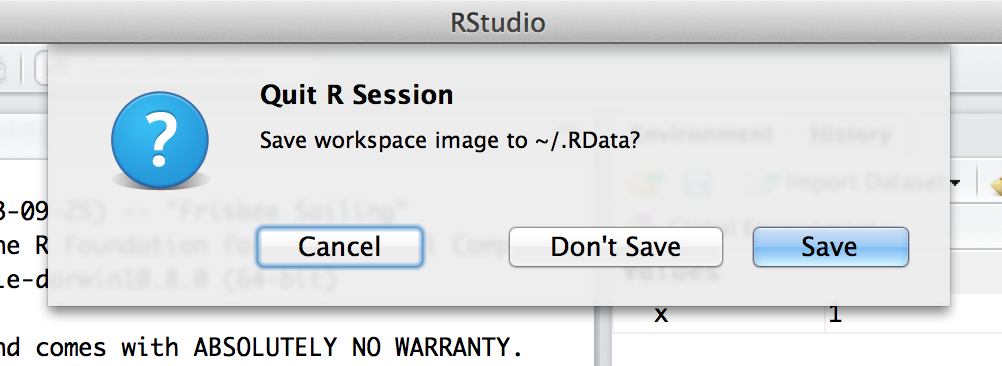
\includegraphics[width=13.92in]{./rbook-master/img/introR/Rstudio_quit} \caption{The dialog box that shows up when you try to close RStudio.}\label{fig:quitR}
\end{figure}

There's one last thing I should cover in this chapter: how to quit R.
When I say this, I'm not trying to imply that R is some kind of
pathological addition and that you need to call the R QuitLine or wear
patches to control the cravings (although you certainly might argue that
there's something seriously pathological about being addicted to R). I
just mean how to exit the program. Assuming you're running R in the
usual way (i.e., through RStudio or the default GUI on a Windows or Mac
computer), then you can just shut down the application in the normal
way. However, R also has a function, called \texttt{q()} that you can
use to quit, which is pretty handy if you're running R in a terminal
window.

Regardless of what method you use to quit R, when you do so for the
first time R will probably ask you if you want to save the ``workspace
image''. We'll talk a lot more about loading and saving data in
Section\ref{load}, but I figured we'd better quickly cover this now
otherwise you're going to get annoyed when you close R at the end of the
chapter. If you're using RStudio, you'll see a dialog box that looks
like the one shown in Figure \ref{fig:quitR}. If you're using a text
based interface you'll see this:

\begin{Shaded}
\begin{Highlighting}[]
\KeywordTok{q}\NormalTok{()}

\NormalTok{## Save workspace image? [y/n/c]: }
\end{Highlighting}
\end{Shaded}

The \texttt{y/n/c} part here is short for ``yes / no / cancel''. Type
\texttt{y} if you want to save, \texttt{n} if you don't, and \texttt{c}
if you've changed your mind and you don't want to quit after all.

What does this actually \emph{mean}? What's going on is that R wants to
know if you want to save all those variables that you've been creating,
so that you can use them later. This sounds like a great idea, so it's
really tempting to type \texttt{y} or click the ``Save'' button. To be
honest though, I very rarely do this, and it kind of annoys me a little
bit\ldots{} what R is \emph{really} asking is if you want it to store
these variables in a ``default'' data file, which it will automatically
reload for you next time you open R. And quite frankly, if I'd wanted to
save the variables, then I'd have already saved them before trying to
quit. Not only that, I'd have saved them to a location of \emph{my}
choice, so that I can find it again later. So I personally never bother
with this.

In fact, every time I install R on a new machine one of the first things
I do is change the settings so that it never asks me again. You can do
this in RStudio really easily: use the menu system to find the RStudio
option; the dialog box that comes up will give you an option to tell R
never to whine about this again (see Figure \ref{fig:RStudiooptions}. On
a Mac, you can open this window by going to the ``RStudio'' menu and
selecting ``Preferences''. On a Windows machine you go to the ``Tools''
menu and select ``Global Options''. Under the ``General'' tab you'll see
an option that reads ``Save workspace to .Rdata on exit''. By default
this is set to ``ask''. If you want R to stop asking, change it to
``never''.

\begin{Shaded}
\begin{Highlighting}[]
\NormalTok{knitr}\OperatorTok{::}\KeywordTok{include_graphics}\NormalTok{(}\StringTok{"./rbook-master/img/introR/Rstudio_options.png"}\NormalTok{)}
\end{Highlighting}
\end{Shaded}

\begin{figure}
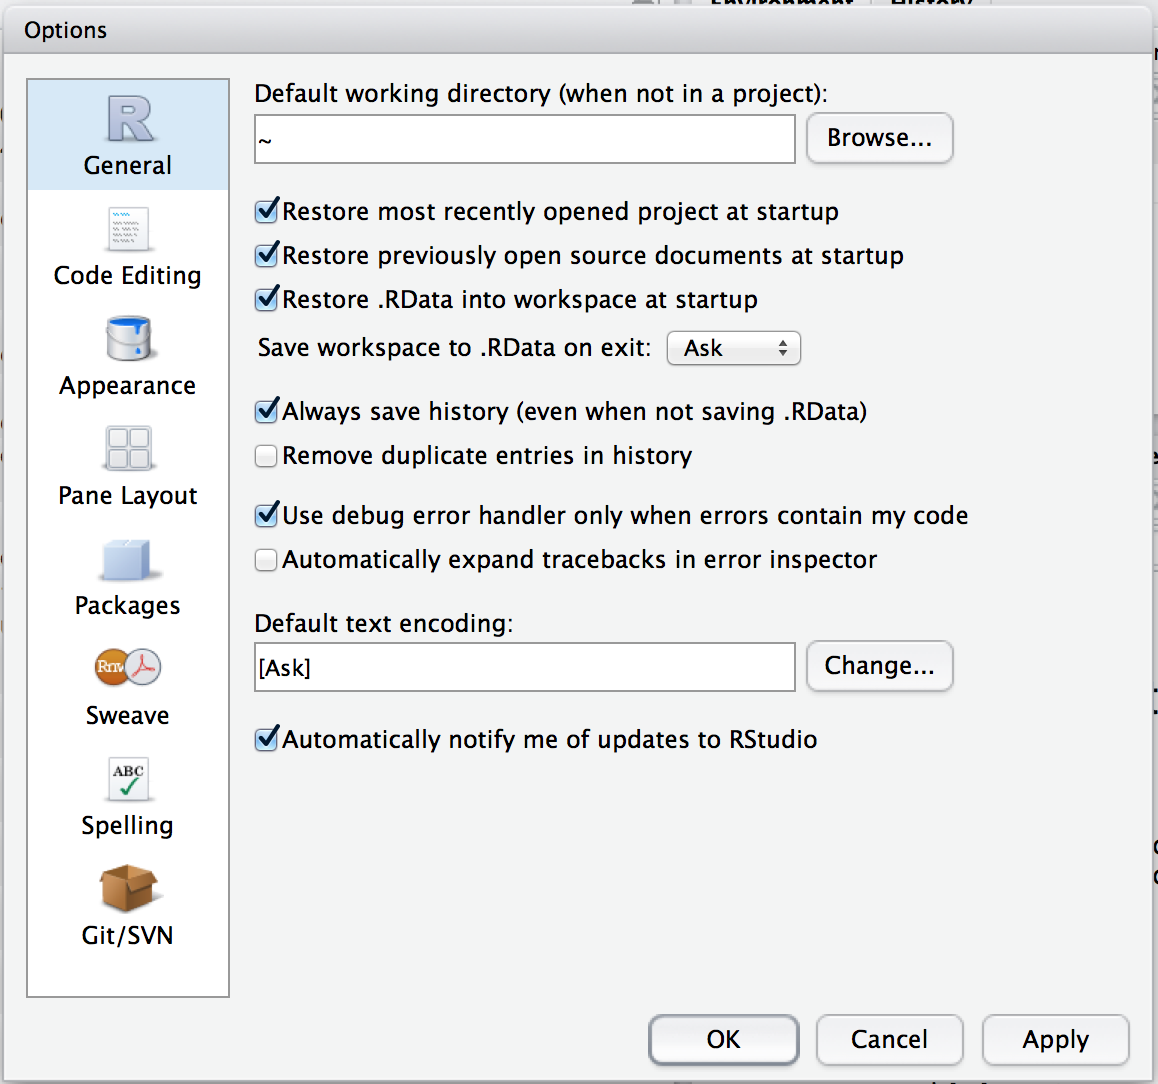
\includegraphics[width=16.08in]{./rbook-master/img/introR/Rstudio_options} \caption{The options window in RStudio. On a Mac, you can open this window by going to the "RStudio" menu and selecting "Preferences". On a Windows machine you go to the "Tools" menu and select "Global Options"}\label{fig:RStudiooptions}
\end{figure}

\section{Summary}\label{summary-1}

Every book that tries to introduce basic programming ideas to novices
has to cover roughly the same topics, and in roughly the same order.
Mine is no exception, and so in the grand tradition of doing it just the
same way everyone else did it, this chapter covered the following
topics:

\begin{itemize}
\tightlist
\item
  \protect\hyperlink{gettingR}{Getting started}. We downloaded and
  installed R and RStudio
\item
  \protect\hyperlink{arithmetic}{Basic commands}. We talked a bit about
  the logic of how R works and in particular how to type commands into
  the R console (Section@ref(\#firstcommand), and in doing so learned
  how to perform basic calculations using the arithmetic operators
  \texttt{+}, \texttt{-}, \texttt{*}, \texttt{/} and \texttt{\^{}}.
\item
  \protect\hyperlink{usingfunctions}{Introduction to functions}. We saw
  several different functions, three that are used to perform numeric
  calculations (\texttt{sqrt()}, \texttt{abs()}, \texttt{round()}, one
  that applies to text (\texttt{nchar()}; Section@ref(\#simpletext), and
  one that works on any variable (\texttt{length()};
  Section@ref(\#veclength). In doing so, we talked a bit about how
  argument names work, and learned about default values for arguments.
  (Section@ref(\#functionarguments)
\item
  Introduction to variables. We learned the basic idea behind variables,
  and how to assign values to variables using the assignment operator
  \texttt{\textless{}-} (Section@ref(\#assign). We also learned how to
  create vectors using the combine function \texttt{c()}.
  (Section@ref(\#vectors)
\item
  Data types. Learned the distinction between numeric, character and
  logical data; including the basics of how to enter and use each of
  them. (Sections@ref(\#assign) to Sections\ref{logicals}
\item
  \protect\hyperlink{logical-operations}{Logical
  operations}.(\#logicals) Learned how to use the logical operators
  \texttt{==}, \texttt{!=}, \texttt{\textless{}},
  \texttt{\textgreater{}}, \texttt{\textless{}=},
  \texttt{=\textgreater{}}, \texttt{!}, \texttt{\&} and
  \texttt{\textbar{}}. And learned how to use logical indexing. (Section
  \ref{indexing}
\end{itemize}

We still haven't arrived at anything that resembles a ``data set'', of
course. Maybe the next Chapter will get us a bit closer\ldots{}

\chapter{Additional R concepts}\label{mechanics}

\begin{quote}
\emph{Form follows function}

-- Louis Sullivan
\end{quote}

In Chapter \ref{introR} our main goal was to get started in R. As we go
through the book we'll run into a lot of new R concepts, which I'll
explain alongside the relevant data analysis concepts. However, there's
still quite a few things that I need to talk about now, otherwise we'll
run into problems when we start trying to work with data and do
statistics. So that's the goal in this chapter: to build on the
introductory content from the last chapter, to get you to the point that
we can start using R for statistics. Broadly speaking, the chapter comes
in two parts. The first half of the chapter is devoted to the
``mechanics'' of R: installing and loading packages, managing the
workspace, navigating the file system, and loading and saving data. In
the second half, I'll talk more about what kinds of variables exist in
R, and introduce three new kinds of variables: factors, data frames and
formulas. I'll finish up by talking a little bit about the help
documentation in R as well as some other avenues for finding assistance.
In general, I'm not trying to be comprehensive in this chapter, I'm
trying to make sure that you've got the basic foundations needed to
tackle the content that comes later in the book. However, a lot of the
topics are revisited in more detail later, especially in Chapters
\ref{datahandling} and \ref{scripting}.

\section{Using comments}\label{comments}

Before discussing any of the more complicated stuff, I want to introduce
the \textbf{\emph{comment}} character, \texttt{\#}. It has a simple
meaning: it tells R to ignore everything else you've written on this
line. You won't have much need of the \texttt{\#} character immediately,
but it's very useful later on when writing scripts (see Chapter
\ref{scripting}). However, while you don't need to use it, I want to be
able to include comments in my R extracts. For instance, if you read
this:\footnote{Notice that I used \texttt{print(keeper)} rather than
  just typing \texttt{keeper}. Later on in the text I'll sometimes use
  the \texttt{print()} function to display things because I think it
  helps make clear what I'm doing, but in practice people rarely do
  this.}

\begin{Shaded}
\begin{Highlighting}[]
\NormalTok{seeker <-}\StringTok{ }\FloatTok{3.1415}           \CommentTok{# create the first variable}
\NormalTok{lover <-}\StringTok{ }\FloatTok{2.7183}            \CommentTok{# create the second variable}
\NormalTok{keeper <-}\StringTok{ }\NormalTok{seeker }\OperatorTok{*}\StringTok{ }\NormalTok{lover   }\CommentTok{# now multiply them to create a third one}
\KeywordTok{print}\NormalTok{( keeper )            }\CommentTok{# print out the value of 'keeper'}
\end{Highlighting}
\end{Shaded}

\begin{verbatim}
## [1] 8.539539
\end{verbatim}

it's a lot easier to understand what I'm doing than if I just write
this:

\begin{Shaded}
\begin{Highlighting}[]
\NormalTok{seeker <-}\StringTok{ }\FloatTok{3.1415}
\NormalTok{lover <-}\StringTok{ }\FloatTok{2.7183}
\NormalTok{keeper <-}\StringTok{ }\NormalTok{seeker }\OperatorTok{*}\StringTok{ }\NormalTok{lover}
\KeywordTok{print}\NormalTok{( keeper )    }
\end{Highlighting}
\end{Shaded}

\begin{verbatim}
## [1] 8.539539
\end{verbatim}

You might have already noticed that the code extracts in Chapter
\ref{introR} included the \texttt{\#} character, but from now on, you'll
start seeing \texttt{\#} characters appearing in the extracts, with some
human-readable explanatory remarks next to them. These are still
perfectly legitimate commands, since R knows that it should ignore the
\texttt{\#} character and everything after it. But hopefully they'll
help make things a little easier to understand.

\section{Installing and loading packages}\label{packageinstall}

In this section I discuss R \textbf{\emph{packages}}, since almost all
of the functions you might want to use in R come in packages. A package
is basically just a big collection of functions, data sets and other R
objects that are all grouped together under a common name. Some packages
are already installed when you put R on your computer, but the vast
majority of them of R packages are out there on the internet, waiting
for you to download, install and use them.

When I first started writing this book, Rstudio didn't really exist as a
viable option for using R, and as a consequence I wrote a very lengthy
section that explained how to do package management using raw R
commands. It's not actually terribly hard to work with packages that
way, but it's clunky and unpleasant. Fortunately, we don't have to do
things that way anymore. In this section, I'll describe how to work with
packages using the Rstudio tools, because they're so much simpler. Along
the way, you'll see that whenever you get Rstudio to do something (e.g.,
install a package), you'll actually see the R commands that get created.
I'll explain them as we go, because I think that helps you understand
what's going on.

However, before we get started, there's a critical distinction that you
need to understand, which is the difference between having a package
\textbf{\emph{installed}} on your computer, and having a package
\textbf{\emph{loaded}} in R. As of this writing, there are just over
5000 R packages freely available ``out there'' on the
internet.\footnote{More precisely, there are 5000 or so packages on
  CRAN, the Comprehensive R Archive Network.} When you install R on your
computer, you don't get all of them: only about 30 or so come bundled
with the basic R installation. So right now there are about 30 packages
``installed'' on your computer, and another 5000 or so that are not
installed. So that's what installed means: it means ``it's on your
computer somewhere''. The critical thing to remember is that just
because something is on your computer doesn't mean R can use it. In
order for R to be able to \emph{use} one of your 30 or so installed
packages, that package must also be ``loaded''. Generally, when you open
up R, only a few of these packages (about 7 or 8) are actually loaded.
Basically what it boils down to is this:

\begin{quote}
A package must be installed before it can be loaded.
\end{quote}

\begin{quote}
A package must be loaded before it can be used.
\end{quote}

This two step process might seem a little odd at first, but the
designers of R had very good reasons to do it this way,\footnote{Basically,
  the reason is that there are 5000 packages, and probably about 4000
  authors of packages, and no-one really knows what all of them do.
  Keeping the installation separate from the loading minimizes the
  chances that two packages will interact with each other in a nasty
  way.} and you get the hang of it pretty quickly.

\subsection{The package panel in
Rstudio}\label{the-package-panel-in-rstudio}

\begin{figure}
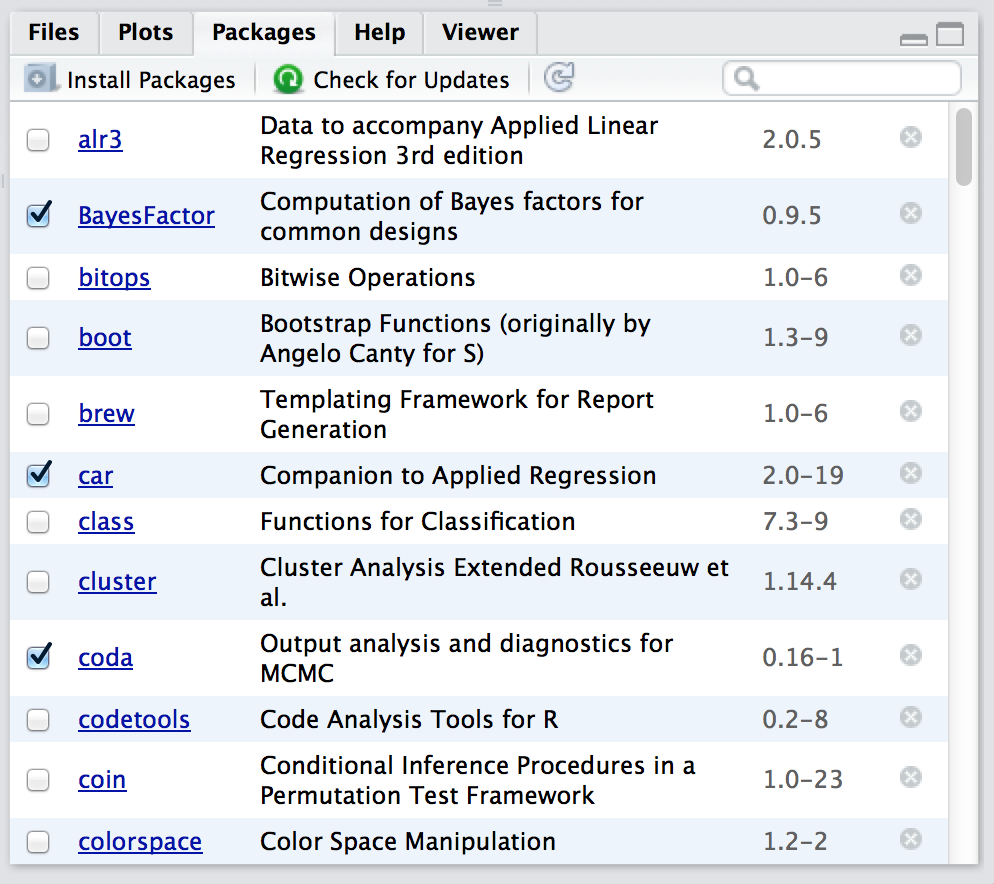
\includegraphics[width=13.81in]{./rbook-master/img/mechanics/Rstudiopackages} \caption{The packages panel.}\label{fig:packagepanel}
\end{figure}

Right, lets get started. The first thing you need to do is look in the
lower right hand panel in Rstudio. You'll see a tab labelled
``Packages''. Click on the tab, and you'll see a list of packages that
looks something like Figure \ref{fig:packagepanel}. Every row in the
panel corresponds to a different package, and every column is a useful
piece of information about that package.\footnote{If you're using the
  command line, you can get the same information by typing
  \texttt{library()} at the command line.} Going from left to right,
here's what each column is telling you:

\begin{itemize}
\tightlist
\item
  The check box on the far left column indicates whether or not the
  package is loaded.
\item
  The one word of text immediately to the right of the check box is the
  name of the package.
\item
  The short passage of text next to the name is a brief description of
  the package.
\item
  The number next to the description tells you what version of the
  package you have installed.
\item
  The little x-mark next to the version number is a button that you can
  push to uninstall the package from your computer (you almost never
  need this).
\end{itemize}

\subsection{Loading a package}\label{packageload}

That seems straightforward enough, so let's try loading and unloading
packades. For this example, I'll use the \texttt{foreign} package. The
\texttt{foreign} package is a collection of tools that are very handy
when R needs to interact with files that are produced by other software
packages (e.g., SPSS). It comes bundled with R, so it's one of the ones
that you have installed already, but it won't be one of the ones loaded.
Inside the \texttt{foreign} package is a function called
\texttt{read.spss()}. It's a handy little function that you can use to
import an SPSS data file into R, so let's pretend we want to use it.
Currently, the \texttt{foreign} package isn't loaded, so if I ask R to
tell me if it knows about a function called \texttt{read.spss()} it
tells me that there's no such thing\ldots{}

\begin{Shaded}
\begin{Highlighting}[]
\KeywordTok{exists}\NormalTok{( }\StringTok{"read.spss"}\NormalTok{ )}
\end{Highlighting}
\end{Shaded}

\begin{verbatim}
## [1] FALSE
\end{verbatim}

Now let's load the package. In Rstudio, the process is dead simple: go
to the package tab, find the entry for the \texttt{foreign} package, and
check the box on the left hand side. The moment that you do this, you'll
see a command like this appear in the R console:

\begin{Shaded}
\begin{Highlighting}[]
\KeywordTok{library}\NormalTok{(}\StringTok{"foreign"}\NormalTok{, }\DataTypeTok{lib.loc=}\StringTok{"/Library/Frameworks/R.framework/Versions/3.0/Resources/library"}\NormalTok{)}
\end{Highlighting}
\end{Shaded}

The \texttt{lib.loc} bit will look slightly different on Macs versus on
Windows, because that part of the command is just Rstudio telling R
where to look to find the installed packages. What I've shown you above
is the Mac version. On a Windows machine, you'll probably see something
that looks like this:

\begin{Shaded}
\begin{Highlighting}[]
\KeywordTok{library}\NormalTok{(}\StringTok{"foreign"}\NormalTok{, }\DataTypeTok{lib.loc=}\StringTok{"C:/Program Files/R/R-3.0.2/library"}\NormalTok{)}
\end{Highlighting}
\end{Shaded}

But actually it doesn't matter much. The \texttt{lib.loc} bit is almost
always unnecessary. Unless you've taken to installing packages in
idiosyncratic places (which is something that you can do if you really
want) R already knows where to look. So in the vast majority of cases,
the command to load the \texttt{foreign} package is just this:

\begin{Shaded}
\begin{Highlighting}[]
\KeywordTok{library}\NormalTok{(}\StringTok{"foreign"}\NormalTok{)}
\end{Highlighting}
\end{Shaded}

Throughout this book, you'll often see me typing in \texttt{library()}
commands. You don't actually have to type them in yourself: you can use
the Rstudio package panel to do all your package loading for you. The
only reason I include the \texttt{library()} commands sometimes is as a
reminder to you to make sure that you have the relevant package loaded.
Oh, and I suppose we should check to see if our attempt to load the
package actually worked. Let's see if R now knows about the existence of
the \texttt{read.spss()} function\ldots{}

\begin{Shaded}
\begin{Highlighting}[]
\KeywordTok{exists}\NormalTok{( }\StringTok{"read.spss"}\NormalTok{ )}
\end{Highlighting}
\end{Shaded}

\begin{verbatim}
## [1] TRUE
\end{verbatim}

Yep. All good.

\subsection{Unloading a package}\label{packageunload}

Sometimes, especially after a long session of working with R, you find
yourself wanting to get rid of some of those packages that you've
loaded. The Rstudio package panel makes this exactly as easy as loading
the package in the first place. Find the entry corresponding to the
package you want to unload, and uncheck the box. When you do that for
the \texttt{foreign} package, you'll see this command appear on screen:

\begin{Shaded}
\begin{Highlighting}[]
\KeywordTok{detach}\NormalTok{(}\StringTok{"package:foreign"}\NormalTok{, }\DataTypeTok{unload=}\OtherTok{TRUE}\NormalTok{)}
\end{Highlighting}
\end{Shaded}

\begin{verbatim}
## Warning: 'foreign' namespace cannot be unloaded:
##   namespace 'foreign' is imported by 'rio', 'psych' so cannot be unloaded
\end{verbatim}

And the package is unloaded. We can verify this by seeing if the
\texttt{read.spss()} function still \texttt{exists()}:

\begin{Shaded}
\begin{Highlighting}[]
\KeywordTok{exists}\NormalTok{( }\StringTok{"read.spss"}\NormalTok{ )}
\end{Highlighting}
\end{Shaded}

\begin{verbatim}
## [1] FALSE
\end{verbatim}

Nope. Definitely gone.

\subsection{A few extra comments}\label{a-few-extra-comments}

Sections \ref{packageload} and \ref{packageunload} cover the main things
you need to know about loading and unloading packages. However, there's
a couple of other details that I want to draw your attention to. A
concrete example is the best way to illustrate. One of the other
packages that you already have installed on your computer is the
\texttt{Matrix} package, so let's load that one and see what happens:

\begin{Shaded}
\begin{Highlighting}[]
\KeywordTok{library}\NormalTok{( Matrix )}

\NormalTok{## Loading required package: lattice}
\end{Highlighting}
\end{Shaded}

This is slightly more complex than the output that we got last time, but
it's not too complicated. The \texttt{Matrix} package makes use of some
of the tools in the \texttt{lattice} package, and R has kept track of
this dependency. So when you try to load the \texttt{Matrix} package, R
recognises that you're also going to need to have the \texttt{lattice}
package loaded too. As a consequence, \emph{both} packages get loaded,
and R prints out a helpful little note on screen to tell you that it's
done so.

R is pretty aggressive about enforcing these dependencies. Suppose, for
example, I try to unload the \texttt{lattice} package while the
\texttt{Matrix} package is still loaded. This is easy enough to try: all
I have to do is uncheck the box next to ``lattice'' in the packages
panel. But if I try this, here's what happens:

\begin{Shaded}
\begin{Highlighting}[]
\KeywordTok{detach}\NormalTok{(}\StringTok{"package:lattice"}\NormalTok{, }\DataTypeTok{unload=}\OtherTok{TRUE}\NormalTok{)}

\NormalTok{## Error: package `lattice' is required by `Matrix' so will not be detached}
\end{Highlighting}
\end{Shaded}

R refuses to do it. This can be quite useful, since it stops you from
accidentally removing something that you still need. So, if I want to
remove both \texttt{Matrix} and \texttt{lattice}, I need to do it in the
correct order

Something else you should be aware of. Sometimes you'll attempt to load
a package, and R will print out a message on screen telling you that
something or other has been ``masked''. This will be confusing to you if
I don't explain it now, and it actually ties very closely to the whole
reason why R forces you to load packages separately from installing
them. Here's an example. Two of the package that I'll refer to a lot in
this book are called \texttt{car} and \texttt{psych}. The \texttt{car}
package is short for ``Companion to Applied Regression'' (which is a
really great book, I'll add), and it has a lot of tools that I'm quite
fond of. The \texttt{car} package was written by a guy called John Fox,
who has written a lot of great statistical tools for social science
applications. The \texttt{psych} package was written by William Revelle,
and it has a lot of functions that are very useful for psychologists in
particular, especially in regards to psychometric techniques. For the
most part, \texttt{car} and \texttt{psych} are quite unrelated to each
other. They do different things, so not surprisingly almost all of the
function names are different. But\ldots{} there's one exception to that.
The \texttt{car} package and the \texttt{psych} package \emph{both}
contain a function called \texttt{logit()}.\footnote{The logit function
  a simple mathematical function that happens not to have been included
  in the basic R distribution.} This creates a naming conflict. If I
load both packages into R, an ambiguity is created. If the user types in
\texttt{logit(100)}, should R use the \texttt{logit()} function in the
\texttt{car} package, or the one in the \texttt{psych} package? The
answer is: R uses whichever package you loaded most recently, and it
tells you this very explicitly. Here's what happens when I load the
\texttt{car} package, and then afterwards load the \texttt{psych}
package:

\begin{Shaded}
\begin{Highlighting}[]
\KeywordTok{library}\NormalTok{(car)}
\KeywordTok{library}\NormalTok{(psych)}
\end{Highlighting}
\end{Shaded}

The output here is telling you that the \texttt{logit} object (i.e.,
function) in the \texttt{car} package is no longer accessible to you.
It's been hidden (or ``masked'') from you by the one in the
\texttt{psych} package.\footnote{Tip for advanced users. You can get R
  to use the one from the \texttt{car} package by using
  \texttt{car::logit()} as your command rather than \texttt{logit()},
  since the \texttt{car::} part tells R explicitly which package to use.
  See also \texttt{:::} if you're especially keen to force R to use
  functions it otherwise wouldn't, but take care, since \texttt{:::} can
  be dangerous.}

\subsection{Downloading new packages}\label{downloading-new-packages}

One of the main selling points for R is that there are thousands of
packages that have been written for it, and these are all available
online. So whereabouts online are these packages to be found, and how do
we download and install them? There is a big repository of packages
called the ``Comprehensive R Archive Network'' (CRAN), and the easiest
way of getting and installing a new package is from one of the many CRAN
mirror sites. Conveniently for us, R provides a function called
\texttt{install.packages()} that you can use to do this. Even
\emph{more} conveniently, the Rstudio team runs its own CRAN mirror and
Rstudio has a clean interface that lets you install packages without
having to learn how to use the \texttt{install.packages()}
command\footnote{It is not very difficult.}

Using the Rstudio tools is, again, dead simple. In the top left hand
corner of the packages panel (Figure \ref{fig:packagepanel}) you'll see
a button called ``Install Packages''. If you click on that, it will
bring up a window like the one shown in Figure
\ref{fig:packageinstalla}.

\begin{figure}
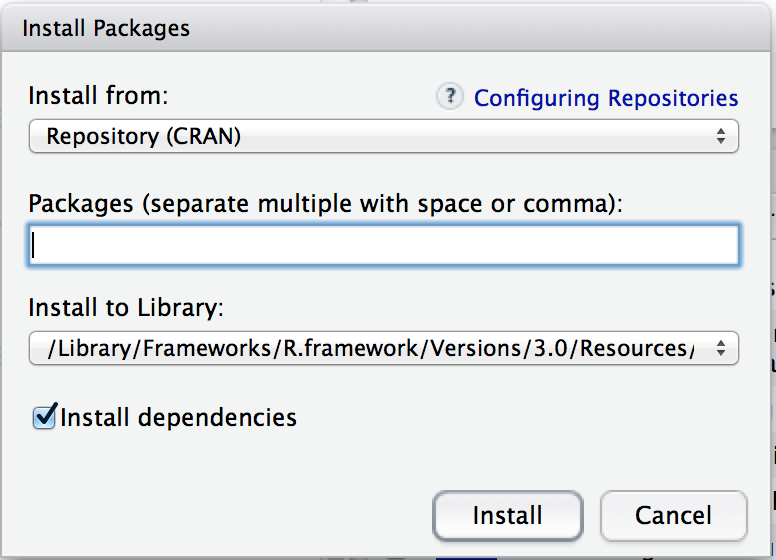
\includegraphics[width=10.78in]{./rbook-master/img/mechanics/installpackage} \caption{The package installation dialog box in Rstudio}\label{fig:packageinstalla}
\end{figure}

There are a few different buttons and boxes you can play with. Ignore
most of them. Just go to the line that says ``Packages'' and start
typing the name of the package that you want. As you type, you'll see a
dropdown menu appear (Figure \ref{fig:packageinstallb}), listing names
of packages that start with the letters that you've typed so far.

\begin{figure}
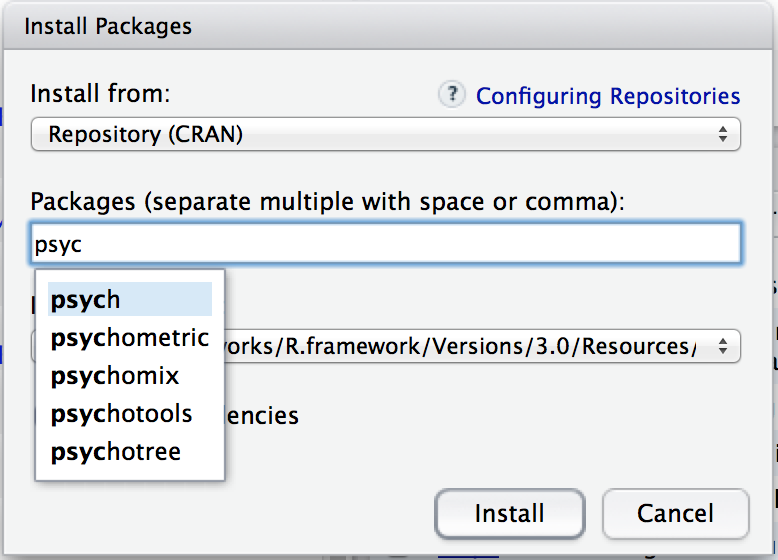
\includegraphics[width=10.81in]{./rbook-master/img/mechanics/installpackage2} \caption{When you start typing, you'll see a dropdown menu suggest a list of possible packages that you might want to install}\label{fig:packageinstallb}
\end{figure}

You can select from this list, or just keep typing. Either way, once
you've got the package name that you want, click on the install button
at the bottom of the window. When you do, you'll see the following
command appear in the R console:

\begin{Shaded}
\begin{Highlighting}[]
\KeywordTok{install.packages}\NormalTok{(}\StringTok{"psych"}\NormalTok{)}
\end{Highlighting}
\end{Shaded}

This is the R command that does all the work. R then goes off to the
internet, has a conversation with CRAN, downloads some stuff, and
installs it on your computer. You probably don't care about all the
details of R's little adventure on the web, but the
\texttt{install.packages()} function is rather chatty, so it reports a
bunch of gibberish that you really aren't all that interested in:

\begin{verbatim}
trying URL 'http://cran.rstudio.com/bin/macosx/contrib/3.0/psych_1.4.1.tgz'
Content type 'application/x-gzip' length 2737873 bytes (2.6 Mb)
opened URL
==================================================
downloaded 2.6 Mb


The downloaded binary packages are in
    /var/folders/cl/thhsyrz53g73q0w1kb5z3l_80000gn/T//RtmpmQ9VT3/downloaded_packages
\end{verbatim}

Despite the long and tedious response, all thar really means is ``I've
installed the psych package''. I find it best to humour the talkative
little automaton. I don't actually read any of this garbage, I just
politely say ``thanks'' and go back to whatever I was doing.

\subsection{Updating R and R packages}\label{updating-r-and-r-packages}

Every now and then the authors of packages release updated versions. The
updated versions often add new functionality, fix bugs, and so on. It's
generally a good idea to update your packages periodically. There's an
\texttt{update.packages()} function that you can use to do this, but
it's probably easier to stick with the Rstudio tool. In the packages
panel, click on the ``Update Packages'' button. This will bring up a
window that looks like the one shown in Figure \ref{fig:updatepackages}.
In this window, each row refers to a package that needs to be updated.
You can to tell R which updates you want to install by checking the
boxes on the left. If you're feeling lazy and just want to update
everything, click the ``Select All'' button, and then click the
``Install Updates'' button. R then prints out a \emph{lot} of garbage on
the screen, individually downloading and installing all the new
packages. This might take a while to complete depending on how good your
internet connection is. Go make a cup of coffee. Come back, and all will
be well.

\begin{figure}
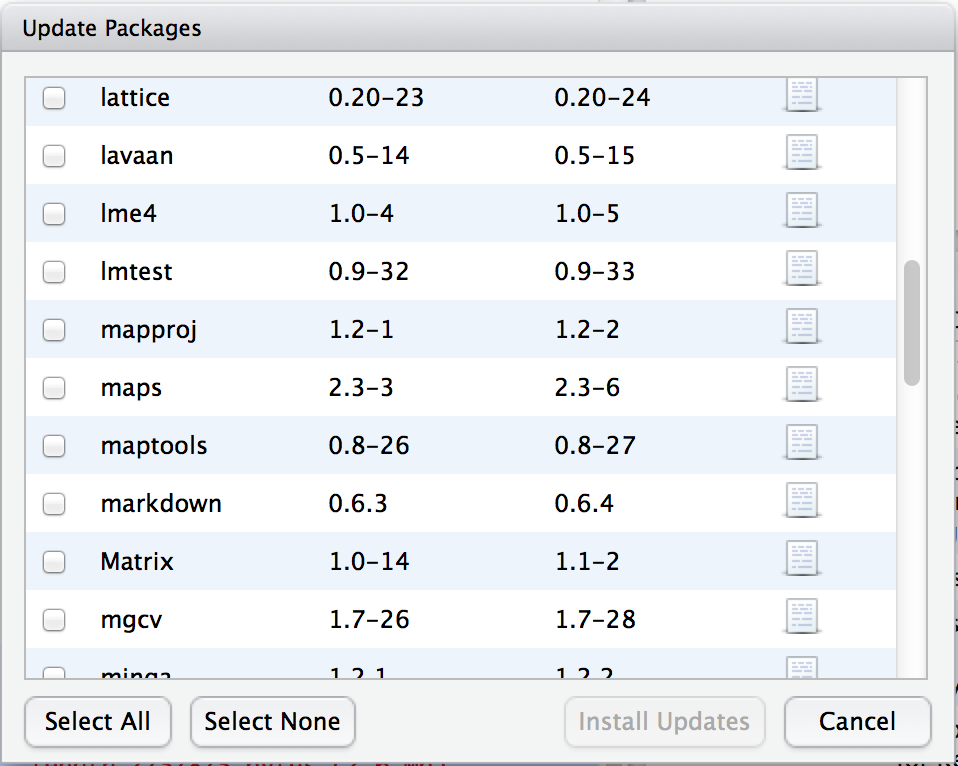
\includegraphics[width=13.31in]{./rbook-master/img/mechanics/updatepackages} \caption{The Rstudio dialog box for updating packages}\label{fig:updatepackages}
\end{figure}

About every six months or so, a new version of R is released. You can't
update R from within Rstudio (not to my knowledge, at least): to get the
new version you can go to the CRAN website and download the most recent
version of R, and install it in the same way you did when you originally
installed R on your computer. This used to be a slightly frustrating
event, because whenever you downloaded the new version of R, you would
lose all the packages that you'd downloaded and installed, and would
have to repeat the process of re-installing them. This was pretty
annoying, and there were some neat tricks you could use to get around
this. However, newer versions of R don't have this problem so I no
longer bother explaining the workarounds for that issue.

\subsection{What packages does this book
use?}\label{what-packages-does-this-book-use}

There are several packages that I make use of in this book. The most
prominent ones are:

\begin{itemize}
\tightlist
\item
  \texttt{lsr}. This is the \emph{Learning Statistics with R} package
  that accompanies this book. It doesn't have a lot of interesting
  high-powered tools: it's just a small collection of handy little
  things that I think can be useful to novice users. As you get more
  comfortable with R this package should start to feel pretty useless to
  you.
\item
  \texttt{psych}. This package, written by William Revelle, includes a
  lot of tools that are of particular use to psychologists. In
  particular, there's several functions that are particularly convenient
  for producing analyses or summaries that are very common in psych, but
  less common in other disciplines.
\item
  \texttt{car}. This is the \emph{Companion to Applied Regression}
  package, which accompanies the excellent book of the same name by
  \citep{Fox2011}. It provides a lot of very powerful tools, only some
  of which we'll touch in this book.
\end{itemize}

Besides these three, there are a number of packages that I use in a more
limited fashion: \texttt{gplots}, \texttt{sciplot}, \texttt{foreign},
\texttt{effects}, \texttt{R.matlab}, \texttt{gdata}, \texttt{lmtest},
and probably one or two others that I've missed. There are also a number
of packages that I refer to but don't actually use in this book, such as
\texttt{reshape}, \texttt{compute.es}, \texttt{HistData} and
\texttt{multcomp} among others. Finally, there are a number of packages
that provide more advanced tools that I hope to talk about in future
versions of the book, such as \texttt{sem}, \texttt{ez}, \texttt{nlme}
and \texttt{lme4}. In any case, whenever I'm using a function that isn't
in the core packages, I'll make sure to note this in the text.

\section{Managing the workspace}\label{workspace}

Let's suppose that you're reading through this book, and what you're
doing is sitting down with it once a week and working through a whole
chapter in each sitting. Not only that, you've been following my advice
and typing in all these commands into R. So far during this chapter,
you'd have typed quite a few commands, although the only ones that
actually involved creating variables were the ones you typed during
Section \ref{comments}. As a result, you currently have three variables;
\texttt{seeker}, \texttt{lover}, and \texttt{keeper}. These three
variables are the contents of your \textbf{\emph{workspace}}, also
referred to as the \textbf{global environment}. The workspace is a key
concept in R, so in this section we'll talk a lot about what it is and
how to manage its contents.

\subsection{Listing the contents of the
workspace}\label{listing-the-contents-of-the-workspace}

\begin{figure}
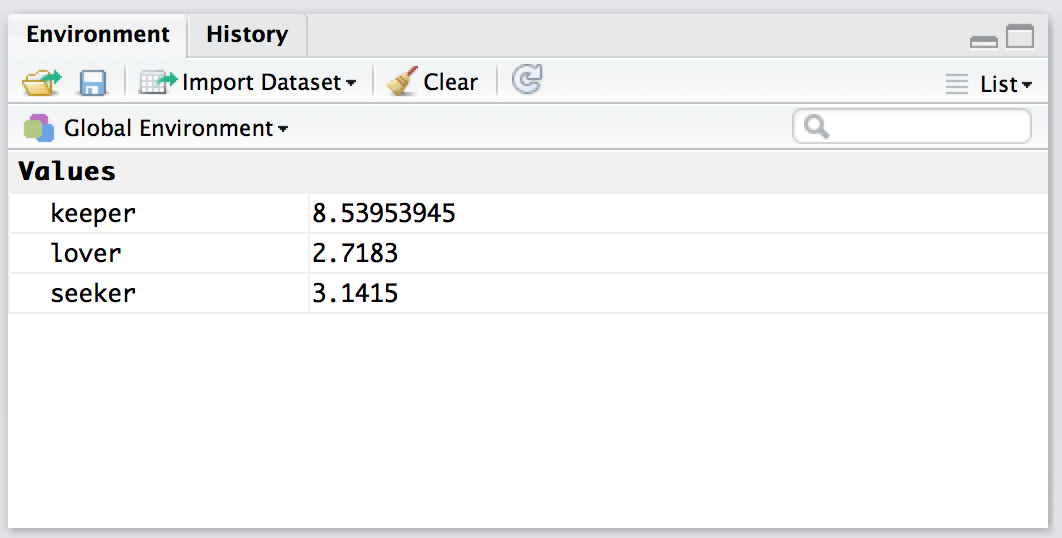
\includegraphics[width=14.75in]{./rbook-master/img/mechanics/workspacepanel} \caption{The Rstudio Environment panel shows you the contents of the workspace. The view shown above is the list view. To switch to the grid view, click on the menu item on the top right that currently reads list. Select grid from the dropdown menu, and then it will switch to a view like the one shown in the other workspace figure}\label{fig:workspace}
\end{figure}

\begin{figure}
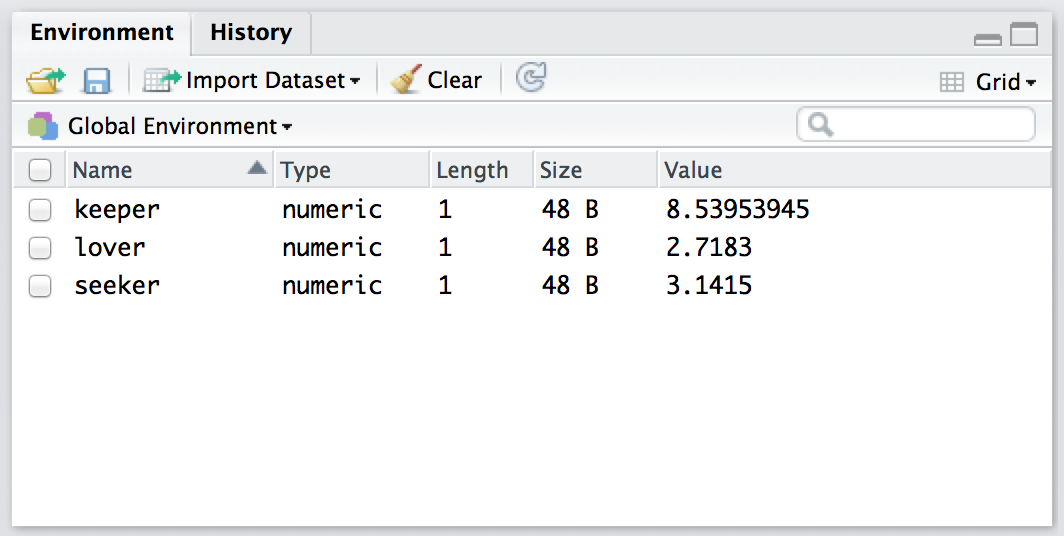
\includegraphics[width=14.78in]{./rbook-master/img/mechanics/workspacepanel2} \caption{The Rstudio "Environment" panel shows you the contents of the workspace. Compare this "grid" view to the "list" earlier}\label{fig:workspace2}
\end{figure}

The first thing that you need to know how to do is examine the contents
of the workspace. If you're using Rstudio, you will probably find that
the easiest way to do this is to use the ``Environment'' panel in the
top right hand corner. Click on that, and you'll see a list that looks
very much like the one shown in Figures \ref{fig:workspace} and
\ref{fig:workspace2}. If you're using the commmand line, then the
\texttt{objects()} function may come in handy:

\begin{Shaded}
\begin{Highlighting}[]
\KeywordTok{objects}\NormalTok{()}
\end{Highlighting}
\end{Shaded}

\begin{verbatim}
##  [1] "any.sales.this.month" "berkeley"             "berkeley.small"      
##  [4] "coef"                 "days.per.month"       "february.sales"      
##  [7] "greeting"             "is.the.Party.correct" "keeper"              
## [10] "lover"                "months"               "profit"              
## [13] "revenue"              "royalty"              "sales"               
## [16] "sales.by.month"       "seeker"               "simpson"             
## [19] "stock.levels"         "x"                    "xlu"
\end{verbatim}

Of course, in the true R tradition, the \texttt{objects()} function has
a lot of fancy capabilities that I'm glossing over in this example.
Moreover there are also several other functions that you can use,
including \texttt{ls()} which is pretty much identical to
\texttt{objects()}, and \texttt{ls.str()} which you can use to get a
fairly detailed description of all the variables in the workspace. In
fact, the \texttt{lsr} package actually includes its own function that
you can use for this purpose, called \texttt{who()}. The reason for
using the \texttt{who()} function is pretty straightforward: in my
everyday work I find that the output produced by the \texttt{objects()}
command isn't \emph{quite} informative enough, because the only thing it
prints out is the name of each variable; but the \texttt{ls.str()}
function is \emph{too} informative, because it prints out a lot of
additional information that I really don't like to look at. The
\texttt{who()} function is a compromise between the two. First, now that
we've got the \texttt{lsr} package installed, we need to load it:

\begin{Shaded}
\begin{Highlighting}[]
\KeywordTok{library}\NormalTok{(lsr)}
\end{Highlighting}
\end{Shaded}

and now we can use the \texttt{who()} function:

\begin{Shaded}
\begin{Highlighting}[]
\KeywordTok{who}\NormalTok{()}
\end{Highlighting}
\end{Shaded}

\begin{verbatim}
##    -- Name --             -- Class --   -- Size --
##    any.sales.this.month   logical       12        
##    berkeley               data.frame    39 x 3    
##    berkeley.small         data.frame    46 x 2    
##    coef                   numeric       2         
##    days.per.month         numeric       12        
##    february.sales         numeric       1         
##    greeting               character     1         
##    is.the.Party.correct   logical       1         
##    keeper                 numeric       1         
##    lover                  numeric       1         
##    months                 character     12        
##    profit                 numeric       12        
##    revenue                numeric       1         
##    royalty                numeric       1         
##    sales                  numeric       1         
##    sales.by.month         numeric       12        
##    seeker                 numeric       1         
##    simpson                matrix        6 x 5     
##    stock.levels           character     12        
##    x                      logical       3         
##    xlu                    numeric       1
\end{verbatim}

As you can see, the \texttt{who()} function lists all the variables and
provides some basic information about what kind of variable each one is
and how many elements it contains. Personally, I find this output much
easier more useful than the very compact output of the
\texttt{objects()} function, but less overwhelming than the extremely
verbose \texttt{ls.str()} function. Throughout this book you'll see me
using the \texttt{who()} function a lot. You don't have to use it
yourself: in fact, I suspect you'll find it easier to look at the
Rstudio environment panel. But for the purposes of writing a textbook I
found it handy to have a nice text based description: otherwise there
would be about another 100 or so screenshots added to the
book.\footnote{This would be especially annoying if you're reading an
  electronic copy of the book because the text displayed by the
  \texttt{who()} function is searchable, whereas text shown in a screen
  shot isn't!}

\subsection{Removing variables from the
workspace}\label{removing-variables-from-the-workspace}

Looking over that list of variables, it occurs to me that I really don't
need them any more. I created them originally just to make a point, but
they don't serve any useful purpose anymore, and now I want to get rid
of them. I'll show you how to do this, but first I want to warn you --
there's no ``undo'' option for variable removal. Once a variable is
removed, it's gone forever unless you save it to disk. I'll show you how
to do \emph{that} in Section \ref{load}, but quite clearly we have no
need for these variables at all, so we can safely get rid of them.

In Rstudio, the easiest way to remove variables is to use the
environment panel. Assuming that you're in grid view (i.e., Figure
\ref{fig:workspace2}), check the boxes next to the variables that you
want to delete, then click on the ``Clear'' button at the top of the
panel. When you do this, Rstudio will show a dialog box asking you to
confirm that you really do want to delete the variables. It's always
worth checking that you really do, because as Rstudio is at pains to
point out, you can't undo this. Once a variable is deleted, it's
gone.\footnote{Mind you, all that means is that it's been removed from
  the workspace. If you've got the data saved to file somewhere, then
  that \emph{file} is perfectly safe.} In any case, if you click
``yes'', that variable will disappear from the workspace: it will no
longer appear in the environment panel, and it won't show up when you
use the \texttt{who()} command.

Suppose you don't access to Rstudio, and you still want to remove
variables. This is where the \textbf{\emph{remove}} function
\texttt{rm()} comes in handy. The simplest way to use \texttt{rm()} is
just to type in a (comma separated) list of all the variables you want
to remove. Let's say I want to get rid of \texttt{seeker} and
\texttt{lover}, but I would like to keep \texttt{keeper}. To do this,
all I have to do is type:

\begin{Shaded}
\begin{Highlighting}[]
\KeywordTok{rm}\NormalTok{( seeker, lover )}
\end{Highlighting}
\end{Shaded}

There's no visible output, but if I now inspect the workspace

\begin{Shaded}
\begin{Highlighting}[]
\KeywordTok{who}\NormalTok{()}
\end{Highlighting}
\end{Shaded}

\begin{verbatim}
##    -- Name --             -- Class --   -- Size --
##    any.sales.this.month   logical       12        
##    berkeley               data.frame    39 x 3    
##    berkeley.small         data.frame    46 x 2    
##    coef                   numeric       2         
##    days.per.month         numeric       12        
##    february.sales         numeric       1         
##    greeting               character     1         
##    is.the.Party.correct   logical       1         
##    keeper                 numeric       1         
##    months                 character     12        
##    profit                 numeric       12        
##    revenue                numeric       1         
##    royalty                numeric       1         
##    sales                  numeric       1         
##    sales.by.month         numeric       12        
##    simpson                matrix        6 x 5     
##    stock.levels           character     12        
##    x                      logical       3         
##    xlu                    numeric       1
\end{verbatim}

I see that there's only the \texttt{keeper} variable left. As you can
see, \texttt{rm()} can be very handy for keeping the workspace tidy.

\section{Navigating the file system}\label{navigation}

In this section I talk a little about how R interacts with the file
system on your computer. It's not a terribly interesting topic, but it's
useful. As background to this discussion, I'll talk a bit about how file
system locations work in Section \ref{filesystem}. Once upon a time
\emph{everyone} who used computers could safely be assumed to understand
how the file system worked, because it was impossible to successfully
use a computer if you didn't! However, modern operating systems are much
more ``user friendly'', and as a consequence of this they go to great
lengths to hide the file system from users. So these days it's not at
all uncommon for people to have used computers most of their life and
not be familiar with the way that computers organise files. If you
already know this stuff, skip straight to Section \ref{navigationR}.
Otherwise, read on. I'll try to give a brief introduction that will be
useful for those of you who have never been forced to learn how to
navigate around a computer using a DOS or UNIX shell.

\subsection{The file system itself}\label{filesystem}

In this section I describe the basic idea behind file locations and file
paths. Regardless of whether you're using Window, Mac OS or Linux, every
file on the computer is assigned a (fairly) human readable address, and
every address has the same basic structure: it describes a \emph{path}
that starts from a \emph{root} location , through as series of
\emph{folders} (or if you're an old-school computer user,
\emph{directories}), and finally ends up at the file.

On a Windows computer the root is the physical drive\footnote{Well, the
  partition, technically.} on which the file is stored, and for most
home computers the name of the hard drive that stores all your files is
C: and therefore most file names on Windows begin with C:. After that
comes the folders, and on Windows the folder names are separated by a
\texttt{\textbackslash{}} symbol. So, the complete path to this book on
my Windows computer might be something like this:

\begin{verbatim}
C:\Users\danRbook\LSR.pdf
\end{verbatim}

and what that \emph{means} is that the book is called LSR.pdf, and it's
in a folder called \texttt{book} which itself is in a folder called dan
which itself is \ldots{} well, you get the idea. On Linux, Unix and Mac
OS systems, the addresses look a little different, but they're more or
less identical in spirit. Instead of using the backslash, folders are
separated using a forward slash, and unlike Windows, they don't treat
the physical drive as being the root of the file system. So, the path to
this book on my Mac might be something like this:

\begin{verbatim}
/Users/dan/Rbook/LSR.pdf
\end{verbatim}

So that's what we mean by the ``path'' to a file. The next concept to
grasp is the idea of a \textbf{\emph{working directory}} and how to
change it. For those of you who have used command line interfaces
previously, this should be obvious already. But if not, here's what I
mean. The working directory is just ``whatever folder I'm currently
looking at''. Suppose that I'm currently looking for files in Explorer
(if you're using Windows) or using Finder (on a Mac). The folder I
currently have open is my user directory (i.e.,
\texttt{C:\textbackslash{}Users\textbackslash{}dan} or
\texttt{/Users/dan}). That's my current working directory.

The fact that we can imagine that the program is ``in'' a particular
directory means that we can talk about moving \emph{from} our current
location \emph{to} a new one. What that means is that we might want to
specify a new location in relation to our current location. To do so, we
need to introduce two new conventions. Regardless of what operating
system you're using, we use . to refer to the current working directory,
and .. to refer to the directory above it. This allows us to specify a
path to a new location in relation to our current location, as the
following examples illustrate. Let's assume that I'm using my Windows
computer, and my working directory is
\texttt{C:\textbackslash{}Users\textbackslash{}danRbook}). The table
below shows several addresses in relation to my current one:

\begin{table}

\caption{\label{tab:unnamed-chunk-110}Basic arithmetic operations in R. These five operators are used very frequently throughout the text, so it's important to be familiar with them at the outset.}
\centering
\begin{tabular}[t]{ll}
\toprule
absolute path (i.e., from root) & relative path (i.e. from C:\textbackslash{}Users\textbackslash{}danRbook)\\
\midrule
C:\textbackslash{}\textbackslash{}Users\textbackslash{}\textbackslash{}dan & ..\\
C:\textbackslash{}\textbackslash{}Users & ..\textbackslash{}\textbackslash{}.. \textbackslash{}\textbackslash{}\\
C:\textbackslash{}\textbackslash{}Users\textbackslash{}\textbackslash{}danRbook\textbackslash{}\textbackslash{}source & .\textbackslash{}\textbackslash{}source\\
C:\textbackslash{}\textbackslash{}Users\textbackslash{}\textbackslash{}dan\textbackslash{}\textbackslash{}nerdstuff & ..\textbackslash{}\textbackslash{}nerdstuff\\
\bottomrule
\end{tabular}
\end{table}

There's one last thing I want to call attention to: the
\texttt{\textasciitilde{}} directory. I normally wouldn't bother, but R
makes reference to this concept sometimes. It's quite common on
computers that have multiple users to define \texttt{\textasciitilde{}}
to be the user's home directory. On my Mac, for instance, the home
directory \texttt{\textasciitilde{}} for the ``dan'' user is
\texttt{\textbackslash{}Users\textbackslash{}dan\textbackslash{}}. And
so, not surprisingly, it is possible to define other directories in
terms of their relationship to the home directory. For example, an
alternative way to describe the location of the \texttt{LSR.pdf} file on
my Mac would be

\begin{verbatim}
~Rbook\LSR.pdf
\end{verbatim}

That's about all you really need to know about file paths. And since
this section already feels too long, it's time to look at how to
navigate the file system in R.

\subsection{Navigating the file system using the R
console}\label{navigationR}

In this section I'll talk about how to navigate this file system from
within R itself. It's not particularly user friendly, and so you'll
probably be happy to know that Rstudio provides you with an easier
method, and I will describe it in Section \ref{nav3}. So in practice,
you won't \emph{really} need to use the commands that I babble on about
in this section, but I do think it helps to see them in operation at
least once before forgetting about them forever.

Okay, let's get started. When you want to load or save a file in R it's
important to know what the working directory is. You can find out by
using the \texttt{getwd()} command. For the moment, let's assume that
I'm using Mac OS or Linux, since there's some subtleties to Windows.
Here's what happens:

\begin{verbatim}
getwd()
## [1] "/Users/dan"
\end{verbatim}

We can change the working directory quite easily using \texttt{setwd()}.
The \texttt{setwd()} function has only the one argument, \texttt{dir},
is a character string specifying a path to a directory, or a path
relative to the working directory. Since I'm currently located at
\texttt{/Users/dan}, the following two are equivalent:

\begin{verbatim}
setwd("/Users/dan/Rbook/data")
setwd("./Rbook/data")
\end{verbatim}

Now that we're here, we can type \texttt{list.files()} command to get a
listing of all the files in that directory. Since this is the directory
in which I store all of the data files that we'll use in this book,
here's what we get as the result:

\begin{verbatim}
list.files()
## [1] "afl24.Rdata"             "aflsmall.Rdata"          "aflsmall2.Rdata"        
## [4] "agpp.Rdata"              "all.zip"                 "annoying.Rdata"         
## [7] "anscombesquartet.Rdata"  "awesome.Rdata"           "awesome2.Rdata"         
## [10] "booksales.csv"           "booksales.Rdata"         "booksales2.csv"         
## [13] "cakes.Rdata"             "cards.Rdata"             "chapek9.Rdata"          
## [16] "chico.Rdata"             "clinicaltrial_old.Rdata" "clinicaltrial.Rdata"    
## [19] "coffee.Rdata"            "drugs.wmc.rt.Rdata"      "dwr_all.Rdata"          
## [22] "effort.Rdata"            "happy.Rdata"             "harpo.Rdata"            
## [25] "harpo2.Rdata"            "likert.Rdata"            "nightgarden.Rdata"      
## [28] "nightgarden2.Rdata"      "parenthood.Rdata"        "parenthood2.Rdata"      
## [31] "randomness.Rdata"        "repeated.Rdata"          "rtfm.Rdata"             
## [34] "salem.Rdata"             "zeppo.Rdata"
\end{verbatim}

Not terribly exciting, I'll admit, but it's useful to know about. In any
case, there's only one more thing I want to make a note of, which is
that R also makes use of the home directory. You can find out what it is
by using the \texttt{path.expand()} function, like this:

\begin{verbatim}
path.expand("~")
## [1] "/Users/dan"
\end{verbatim}

You can change the user directory if you want, but we're not going to
make use of it very much so there's no reason to. The only reason I'm
even bothering to mention it at all is that when you use Rstudio to open
a file, you'll see output on screen that defines the path to the file
relative to the \#\textasciitilde{}\# directory. I'd prefer you not to
be confused when you see it.\footnote{One additional thing worth calling
  your attention to is the \texttt{file.choose()} function. Suppose you
  want to load a file and you don't quite remember where it is, but
  would like to browse for it. Typing \texttt{file.choose()} at the
  command line will open a window in which you can browse to find the
  file; when you click on the file you want, R will print out the full
  path to that file. This is kind of handy.}

\subsection{Why do the Windows paths use the wrong
slash?}\label{why-do-the-windows-paths-use-the-wrong-slash}

Let's suppose I'm on Windows. As before, I can find out what my current
working directory is like this:

\begin{verbatim}
getwd()
## [1] "C:/Users/dan/
\end{verbatim}

This seems about right, but you might be wondering why R is displaying a
Windows path using the wrong type of slash. The answer is slightly
complicated, and has to do with the fact that R treats the
\texttt{\textbackslash{}} character as ``special'' (see Section
\ref{escapechars}). If you're deeply wedded to the idea of specifying a
path using the Windows style slashes, then what you need to do is to
type \texttt{/} whenever you mean \texttt{\textbackslash{}}. In other
words, if you want to specify the working directory on a Windows
computer, you need to use one of the following commands:

\begin{verbatim}
setwd( "C:/Users/dan" )
setwd( "C:\\Users\\dan" )
\end{verbatim}

It's kind of annoying to have to do it this way, but as you'll see later
on in Section \ref{escapechars} it's a necessary evil. Fortunately, as
we'll see in the next section, Rstudio provides a much simpler way of
changing directories\ldots{}

\subsection{Navigating the file system using the Rstudio file
panel}\label{nav3}

Although I think it's important to understand how all this command line
stuff works, in many (maybe even most) situations there's an easier way.
For our purposes, the easiest way to navigate the file system is to make
use of Rstudio's built in tools. The ``file'' panel -- the lower right
hand area in Figure \ref{fig:filepanel} -- is actually a pretty decent
file browser. Not only can you just point and click on the names to move
around the file system, you can also use it to set the working
directory, and even load files.

\begin{figure}
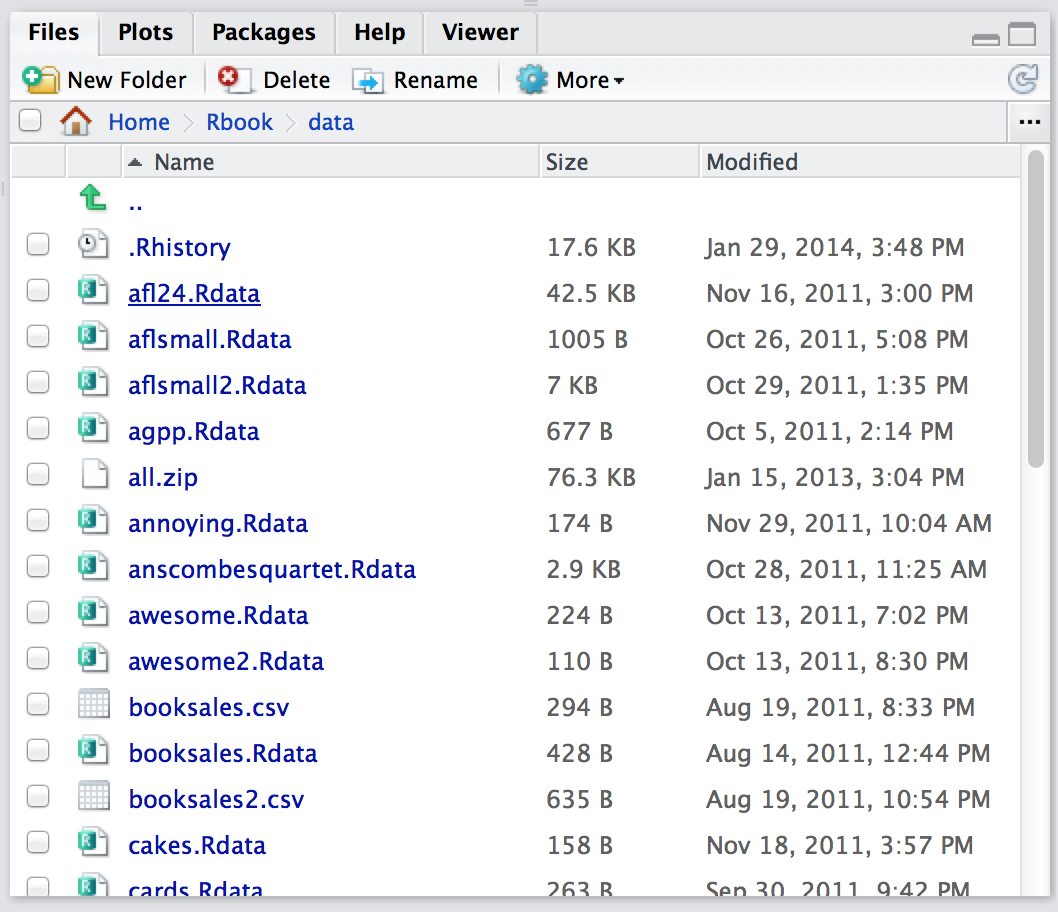
\includegraphics[width=14.69in]{./rbook-master/img/mechanics/filepanel} \caption{The "file panel" is the area shown in the lower right hand corner. It provides a very easy way to browse and navigate your computer using R. See main text for details.}\label{fig:filepanel}
\end{figure}

Here's what you need to do to change the working directory using the
file panel. Let's say I'm looking at the actual screen shown in Figure
\ref{fig:filepanel}. At the top of the file panel you see some text that
says ``Home \(>\) Rbook \(>\) data''. What that means is that it's
\emph{displaying} the files that are stored in the

\begin{verbatim}
/Users/dan/Rbook/data
\end{verbatim}

directory on my computer. It does \emph{not} mean that this is the R
working directory. If you want to change the R working directory, using
the file panel, you need to click on the button that reads ``More''.
This will bring up a little menu, and one of the options will be ``Set
as Working Directory''. If you select that option, then R really will
change the working directory. You can tell that it has done so because
this command appears in the console:

\begin{verbatim}
setwd("~/Rbook/data")
\end{verbatim}

In other words, Rstudio sends a command to the R console, exactly as if
you'd typed it yourself. The file panel can be used to do other things
too. If you want to move ``up'' to the parent folder (e.g., from
\texttt{/Users/dan/Rbook/data} to \texttt{/Users/dan/Rbook} click on the
``..'' link in the file panel. To move to a subfolder, click on the name
of the folder that you want to open. You can open some types of file by
clicking on them. You can delete files from your computer using the
``delete'' button, rename them with the ``rename'' button, and so on.

As you can tell, the file panel is a very handy little tool for
navigating the file system. But it can do more than just navigate. As
we'll see later, it can be used to open files. And if you look at the
buttons and menu options that it presents, you can even use it to
rename, delete, copy or move files, and create new folders. However,
since most of that functionality isn't critical to the basic goals of
this book, I'll let you discover those on your own.

\section{Loading and saving data}\label{load}

There are several different types of files that are likely to be
relevant to us when doing data analysis. There are three in particular
that are especially important from the perspective of this book:

\begin{itemize}
\tightlist
\item
  \emph{Workspace files} are those with a .Rdata file extension. This is
  the standard kind of file that R uses to store data and variables.
  They're called ``workspace files'' because you can use them to save
  your whole workspace.
\item
  \emph{Comma separated value (CSV) files} are those with a .csv file
  extension. These are just regular old text files, and they can be
  opened with almost any software. It's quite typical for people to
  store data in CSV files, precisely because they're so simple.
\item
  \emph{Script files} are those with a .R file extension. These aren't
  data files at all; rather, they're used to save a collection of
  commands that you want R to execute later. They're just text files,
  but we won't make use of them until Chapter \ref{scripting}.
\end{itemize}

There are also several other types of file that R makes use
of,\footnote{Notably those with .rda, .Rd, .Rhistory, .rdb and .rdx
  extensions} but they're not really all that central to our interests.
There are also several other kinds of data file that you might want to
import into R. For instance, you might want to open Microsoft Excel
spreadsheets (.xlsx files), or data files that have been saved in the
native file formats for other statistics software, such as SPSS, SAS,
Minitab, Stata or Systat. Finally, you might have to handle databases. R
tries hard to play nicely with other software, so it has tools that let
you open and work with any of these and many others. I'll discuss some
of these other possibilities elsewhere in this book (Section
\ref{importing}), but for now I want to focus primarily on the two kinds
of data file that you're most likely to need: .Rdata files and .csv
files. In this section I'll talk about how to load a workspace file, how
to import data from a CSV file, and how to save your workspace to a
workspace file. Throughout this section I'll first describe the
(sometimes awkward) R commands that do all the work, and then I'll show
you the (much easier) way to do it using Rstudio.

\subsection{Loading workspace files using
R}\label{loading-workspace-files-using-r}

When I used the \texttt{list.files()} command to list the contents of
the \texttt{/Users/dan/Rbook/data} directory (in Section
\ref{navigationR}), the output referred to a file called
booksales.Rdata. Let's say I want to load the data from this file into
my workspace. The way I do this is with the \texttt{load()} function.
There are two arguments to this function, but the only one we're
interested in is

\begin{itemize}
\tightlist
\item
  \texttt{file}. This should be a character string that specifies a path
  to the file that needs to be loaded. You can use an absolute path or a
  relative path to do so.
\end{itemize}

Using the absolute file path, the command would look like this:

\begin{verbatim}
load( file = "/Users/dan/Rbook/data/booksales.Rdata" )
\end{verbatim}

but this is pretty lengthy. Given that the working directory (remember,
we changed the directory at the end of Section \ref{nav3}) is
\texttt{/Users/dan/Rbook/data}, I could use a relative file path, like
so:

\begin{verbatim}
load( file = "../data/booksales.Rdata" )
\end{verbatim}

However, my preference is usually to change the working directory first,
and \emph{then} load the file. What that would look like is this:

\begin{verbatim}
setwd( "../data" )         # move to the data directory
load( "booksales.Rdata" )  # load the data
\end{verbatim}

If I were then to type \texttt{who()} I'd see that there are several new
variables in my workspace now. Throughout this book, whenever you see me
loading a file, I will assume that the file is actually stored in the
working directory, or that you've changed the working directory so that
R is pointing at the directory that contains the file. Obviously,
\emph{you} don't need type that command yourself: you can use the
Rstudio file panel to do the work.

\subsection{Loading workspace files using
Rstudio}\label{loading-workspace-files-using-rstudio}

Okay, so how do we open an .Rdata file using the Rstudio file panel?
It's terribly simple. First, use the file panel to find the folder that
contains the file you want to load. If you look at Figure
\ref{fig:filepanel}, you can see that there are several .Rdata files
listed. Let's say I want to load the \texttt{booksales.Rdata} file. All
I have to do is click on the file name. Rstudio brings up a little
dialog box asking me to confirm that I do want to load this file. I
click yes. The following command then turns up in the console,

\begin{verbatim}
load("~/Rbook/data/booksales.Rdata")
\end{verbatim}

and the new variables will appear in the workspace (you'll see them in
the Environment panel in Rstudio, or if you type \texttt{who()}). So
easy it barely warrants having its own section.

\subsection{\texorpdfstring{Importing data from CSV files using
\texttt{loadingcsv}}{Importing data from CSV files using loadingcsv}}\label{importing-data-from-csv-files-using-loadingcsv}

One quite commonly used data format is the humble ``comma separated
value'' file, also called a CSV file, and usually bearing the file
extension .csv. CSV files are just plain old-fashioned text files, and
what they store is basically just a table of data. This is illustrated
in Figure \ref{fig:booksalescsv}, which shows a file called
booksales.csv that I've created. As you can see, each row corresponds to
a variable, and each row represents the book sales data for one month.
The first row doesn't contain actual data though: it has the names of
the variables.

\begin{figure}
\centering
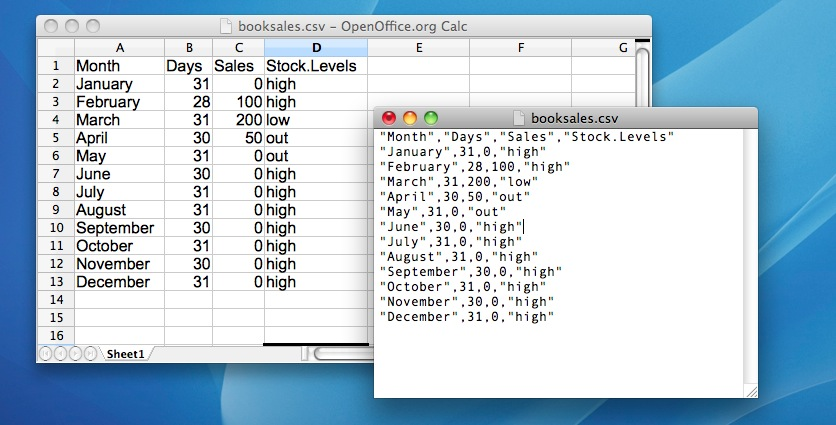
\includegraphics{./rbook-master/img/mechanics/booksalescsv.jpg}
\caption{\label{fig:booksalescsv}The booksales.csv data file. On the left,
I've opened the file in using a spreadsheet program (OpenOffice), which
shows that the file is basically a table. On the right, the same file is
open in a standard text editor (the TextEdit program on a Mac), which
shows how the file is formatted. The entries in the table are wrapped in
quote marks and separated by commas.}
\end{figure}

If Rstudio were not available to you, the easiest way to open this file
would be to use the \texttt{read.csv()} function.\footnote{In a lot of
  books you'll see the \texttt{read.table()} function used for this
  purpose instead of \texttt{read.csv()}. They're more or less identical
  functions, with the same arguments and everything. They differ only in
  the default values.} This function is pretty flexible, and I'll talk a
lot more about it's capabilities in Section \ref{importing} for more
details, but for now there's only two arguments to the function that
I'll mention:

\begin{itemize}
\tightlist
\item
  \texttt{file}. This should be a character string that specifies a path
  to the file that needs to be loaded. You can use an absolute path or a
  relative path to do so.
\item
  \texttt{header}. This is a logical value indicating whether or not the
  first row of the file contains variable names. The default value is
  \texttt{TRUE}.
\end{itemize}

Therefore, to import the CSV file, the command I need is:

\begin{Shaded}
\begin{Highlighting}[]
\NormalTok{books <-}\StringTok{ }\KeywordTok{read.csv}\NormalTok{( }\DataTypeTok{file =} \StringTok{"booksales.csv"}\NormalTok{ )}
\end{Highlighting}
\end{Shaded}

There are two very important points to notice here. Firstly, notice that
I \emph{didn't} try to use the \texttt{load()} function, because that
function is only meant to be used for .Rdata files. If you try to use
\texttt{load()} on other types of data, you get an error. Secondly,
notice that when I imported the CSV file I assigned the result to a
variable, which I imaginatively called \texttt{books}.\footnote{Note
  that I didn't to this in my earlier example when loading the .Rdata}
file. There's a reason for this. The idea behind an \texttt{.Rdata} file
is that it stores a whole workspace. So, if you had the ability to look
inside the file yourself you'd see that the data file keeps track of all
the variables and their names. So when you \texttt{load()} the file, R
restores all those original names. CSV files are treated differently: as
far as R is concerned, the CSV only stores \emph{one} variable, but that
variable is big table. So when you import that table into the workspace,
R expects \emph{you} to give it a name.{]} Let's have a look at what
we've got:

\begin{Shaded}
\begin{Highlighting}[]
\KeywordTok{print}\NormalTok{( books )}
\end{Highlighting}
\end{Shaded}

\begin{verbatim}
##        Month Days Sales Stock.Levels
## 1    January   31     0         high
## 2   February   28   100         high
## 3      March   31   200          low
## 4      April   30    50          out
## 5        May   31     0          out
## 6       June   30     0         high
## 7       July   31     0         high
## 8     August   31     0         high
## 9  September   30     0         high
## 10   October   31     0         high
## 11  November   30     0         high
## 12  December   31     0         high
\end{verbatim}

Clearly, it's worked, but the format of this output is a bit unfamiliar.
We haven't seen anything like this before. What you're looking at is a
\emph{data frame}, which is a very important kind of variable in R, and
one I'll discuss in Section \ref{dataframes}. For now, let's just be
happy that we imported the data and that it looks about right.

\subsection{Importing data from CSV files using
Rstudio}\label{importing-data-from-csv-files-using-rstudio}

Yet again, it's easier in Rstudio. In the environment panel in Rstudio
you should see a button called ``Import Dataset''. Click on that, and it
will give you a couple of options: select the ``From Text File\ldots{}''
option, and it will open up a very familiar dialog box asking you to
select a file: if you're on a Mac, it'll look like the usual Finder
window that you use to choose a file; on Windows it looks like an
Explorer window. An example of what it looks like on a Mac is shown in
Figure \ref{fig:fileopen}. I'm assuming that you're familiar with your
own computer, so you should have no problem finding the CSV file that
you want to import! Find the one you want, then click on the ``Open''
button. When you do this, you'll see a window that looks like the one in
Figure \ref{fig:import}.

\begin{figure}
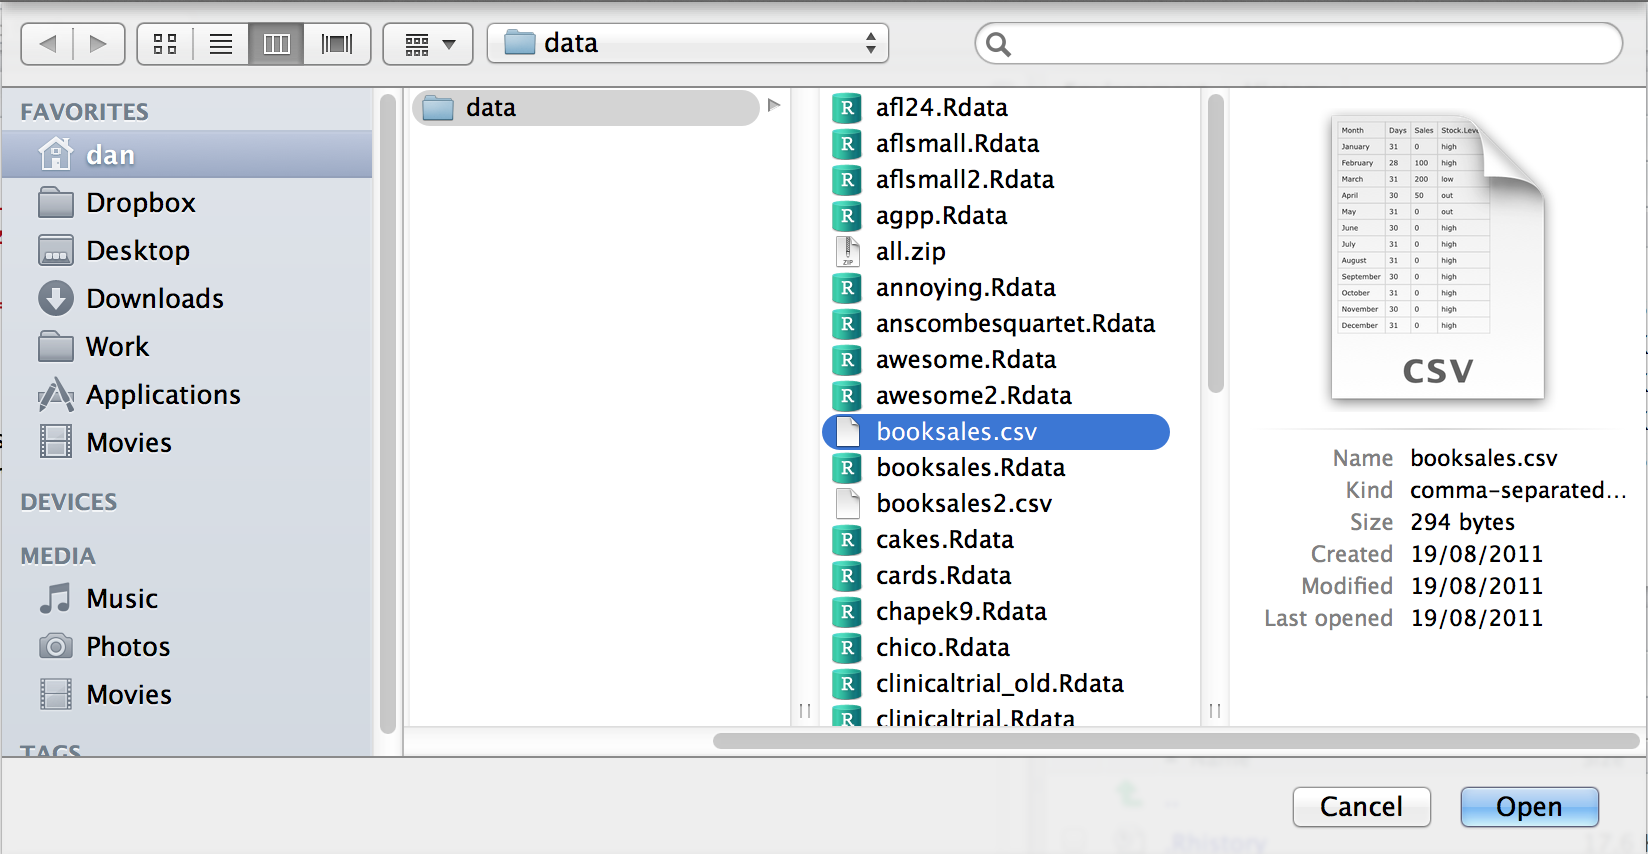
\includegraphics[width=22.89in]{./rbook-master/img/mechanics/openscreen} \caption{A dialog box on a Mac asking you to select the CSV file R should try to import. Mac users will recognise this immediately: it's the usual way in which a Mac asks you to find a file. Windows users won't see this: they'll see the usual explorer window that Windows always gives you when it wants you to select a file.}\label{fig:fileopen}
\end{figure}

The import data set window is relatively straightforward to understand.

\begin{figure}
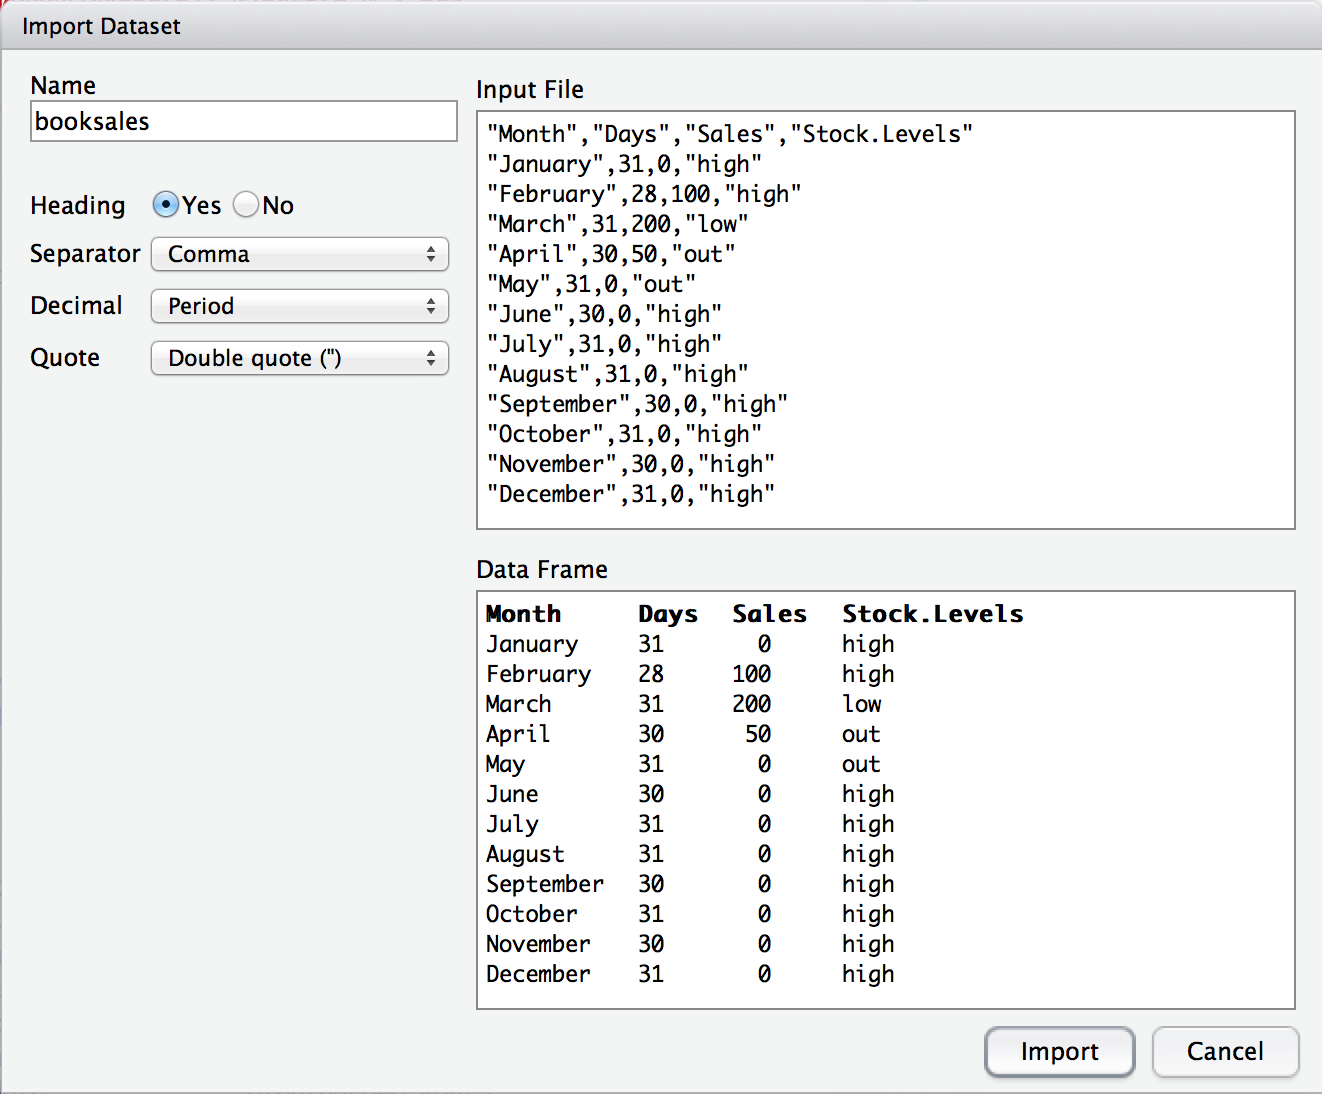
\includegraphics[width=18.36in]{./rbook-master/img/mechanics/import} \caption{The Rstudio window for importing a CSV file into R}\label{fig:import}
\end{figure}

In the top left corner, you need to type the name of the variable you R
to create. By default, that will be the same as the file name: our file
is called \texttt{booksales.csv}, so Rstudio suggests the name
\texttt{booksales}. If you're happy with that, leave it alone. If not,
type something else. Immediately below this are a few things that you
can tweak to make sure that the data gets imported correctly:

\begin{itemize}
\tightlist
\item
  Heading. Does the first row of the file contain raw data, or does it
  contain headings for each variable? The \texttt{booksales.csv} file
  has a header at the top, so I selected ``yes''.
\item
  Separator. What character is used to separate different entries? In
  most CSV files this will be a comma (it is ``comma separated'' after
  all). But you can change this if your file is different.
\item
  Decimal. What character is used to specify the decimal point? In
  English speaking countries, this is almost always a period (i.e.,
  \texttt{.}). That's not universally true: many European countries use
  a comma. So you can change that if you need to.
\item
  Quote. What character is used to denote a block of text? That's
  usually going to be a double quote mark. It is for the
  \texttt{booksales.csv} file, so that's what I selected.
\end{itemize}

The nice thing about the Rstudio window is that it shows you the raw
data file at the top of the window, and it shows you a preview of the
data at the bottom. If the data at the bottom doesn't look right, try
changing some of the settings on the left hand side. Once you're happy,
click ``Import''. When you do, two commands appear in the R console:

\begin{verbatim}
booksales <- read.csv("~/Rbook/data/booksales.csv")
View(booksales)
\end{verbatim}

The first of these commands is the one that loads the data. The second
one will display a pretty table showing the data in Rstudio.

\subsection{\texorpdfstring{Saving a workspace file using
\texttt{save}}{Saving a workspace file using save}}\label{saving-a-workspace-file-using-save}

Not surprisingly, saving data is very similar to loading data. Although
Rstudio provides a simple way to save files (see below), it's worth
understanding the actual commands involved. There are two commands you
can use to do this, \texttt{save()} and \texttt{save.image()}. If you're
happy to save \emph{all} of the variables in your workspace into the
data file, then you should use \texttt{save.image()}. And if you're
happy for R to save the file into the current working directory, all you
have to do is this:

\begin{Shaded}
\begin{Highlighting}[]
\KeywordTok{save.image}\NormalTok{( }\DataTypeTok{file =} \StringTok{"myfile.Rdata"}\NormalTok{ )}
\end{Highlighting}
\end{Shaded}

Since \texttt{file} is the first argument, you can shorten this to
\texttt{save.image("myfile.Rdata")}; and if you want to save to a
different directory, then (as always) you need to be more explicit about
specifying the path to the file, just as we discussed in Section
\ref{navigation}. Suppose, however, I have several variables in my
workspace, and I only want to save some of them. For instance, I might
have this as my workspace:

\begin{Shaded}
\begin{Highlighting}[]
\KeywordTok{who}\NormalTok{()}
\NormalTok{##   -- Name --   -- Class --   -- Size --}
\NormalTok{##   data         data.frame    3 x 2     }
\NormalTok{##   handy        character     1         }
\NormalTok{##   junk         numeric       1        }
\end{Highlighting}
\end{Shaded}

I want to save \texttt{data} and \texttt{handy}, but not \texttt{junk}.
But I don't want to delete \texttt{junk} right now, because I want to
use it for something else later on. This is where the \texttt{save()}
function is useful, since it lets me indicate exactly which variables I
want to save. Here is one way I can use the \texttt{save} function to
solve my problem:

\begin{Shaded}
\begin{Highlighting}[]
\KeywordTok{save}\NormalTok{(data, handy, }\DataTypeTok{file =} \StringTok{"myfile.Rdata"}\NormalTok{)}
\end{Highlighting}
\end{Shaded}

Importantly, you \emph{must} specify the name of the \texttt{file}
argument. The reason is that if you don't do so, R will think that
\texttt{"myfile.Rdata"} is actually a \emph{variable} that you want to
save, and you'll get an error message. Finally, I should mention a
second way to specify which variables the \texttt{save()} function
should save, which is to use the \texttt{list} argument. You do so like
this:

\begin{Shaded}
\begin{Highlighting}[]
\NormalTok{save.me <-}\StringTok{ }\KeywordTok{c}\NormalTok{(}\StringTok{"data"}\NormalTok{, }\StringTok{"handy"}\NormalTok{)   }\CommentTok{# the variables to be saved}
\KeywordTok{save}\NormalTok{( }\DataTypeTok{file =} \StringTok{"booksales2.Rdata"}\NormalTok{, }\DataTypeTok{list =}\NormalTok{ save.me )   }\CommentTok{# the command to save them}
\end{Highlighting}
\end{Shaded}

\subsection{Saving a workspace file using Rstudio}\label{save1}

Rstudio allows you to save the workspace pretty easily. In the
environment panel (Figures \ref{fig:workspace} and \ref{fig:workspace2})
you can see the ``save'' button. There's no text, but it's the same icon
that gets used on every computer everywhere: it's the one that looks
like a floppy disk. You know, those things that haven't been used in
about 20 years. Alternatively, go to the ``Session'' menu and click on
the ``Save Workspace As\ldots{}'' option.\footnote{A word of warning:
  what you \emph{don't} want to do is use the ``File'' menu. If you look
  in the ``File'' menu you will see ``Save'' and ``Save As\ldots{}''
  options, but they don't save the workspace. Those options are used for
  dealing with \emph{scripts}, and so they'll produce \texttt{.R} files.
  We won't get to those until Chapter \ref{scripting}.} This will bring
up the standard ``save'' dialog box for your operating system (e.g., on
a Mac it'll look a little bit like the loading dialog box in Figure
\ref{fig:fileopen}). Type in the name of the file that you want to save
it to, and all the variables in your workspace will be saved to disk.
You'll see an R command like this one

\begin{Shaded}
\begin{Highlighting}[]
\KeywordTok{save.image}\NormalTok{(}\StringTok{"~/Desktop/Untitled.RData"}\NormalTok{)}
\end{Highlighting}
\end{Shaded}

Pretty straightforward, really.

\subsection{Other things you might want to
save}\label{other-things-you-might-want-to-save}

Until now, we've talked mostly about loading and saving \emph{data}.
Other things you might want to save include:

\begin{itemize}
\item
  \emph{The output}. Sometimes you might also want to keep a copy of all
  your interactions with R, including everything that you typed in and
  everything that R did in response. There are some functions that you
  can use to get R to write its output to a file rather than to print
  onscreen (e.g., \texttt{sink()}), but to be honest, if you do want to
  save the R output, the easiest thing to do is to use the mouse to
  select the relevant text in the R console, go to the ``Edit'' menu in
  Rstudio and select ``Copy''. The output has now been copied to the
  clipboard. Now open up your favourite text editor or word processing
  software, and paste it. And you're done. However, this will only save
  the contents of the console, not the plots you've drawn (assuming
  you've drawn some). We'll talk about saving images later on.
\item
  \emph{A script}. While it is possible -- and sometimes handy -- to
  save the R output as a method for keeping a copy of your statistical
  analyses, another option that people use a lot (especially when you
  move beyond simple ``toy'' analyses) is to write \emph{scripts}. A
  script is a text file in which you write out all the commands that you
  want R to run. You can write your script using whatever software you
  like. In real world data analysis writing scripts is a key skill --
  and as you become familiar with R you'll probably find that most of
  what you do involves scripting rather than typing commands at the R
  prompt. However, you won't need to do much scripting initially, so
  we'll leave that until Chapter \ref{scripting}.
\end{itemize}

\section{Useful things to know about variables}\label{useful}

In Chapter \ref{introR} I talked a lot about variables, how they're
assigned and some of the things you can do with them, but there's a lot
of additional complexities. That's not a surprise of course. However,
some of those issues are worth drawing your attention to now. So that's
the goal of this section; to cover a few extra topics. As a consequence,
this section is basically a bunch of things that I want to briefly
mention, but don't really fit in anywhere else. In short, I'll talk
about several different issues in this section, which are only loosely
connected to one another.

\subsection{Special values}\label{specials}

The first thing I want to mention are some of the ``special'' values
that you might see R produce. Most likely you'll see them in situations
where you were expecting a number, but there are quite a few other ways
you can encounter them. These values are \texttt{Inf}, \texttt{NaN},
\texttt{NA} and \texttt{NULL}. These values can crop up in various
different places, and so it's important to understand what they mean.

\begin{itemize}
\tightlist
\item
  \emph{Infinity} (\texttt{Inf}). The easiest of the special values to
  explain is \texttt{Inf}, since it corresponds to a value that is
  infinitely large. You can also have \texttt{-Inf}. The easiest way to
  get \texttt{Inf} is to divide a positive number by 0:
\end{itemize}

\begin{Shaded}
\begin{Highlighting}[]
\DecValTok{1} \OperatorTok{/}\StringTok{ }\DecValTok{0}
\end{Highlighting}
\end{Shaded}

\begin{verbatim}
## [1] Inf
\end{verbatim}

In most real world data analysis situations, if you're ending up with
infinite numbers in your data, then something has gone awry. Hopefully
you'll never have to see them.

\begin{itemize}
\tightlist
\item
  \emph{Not a Number} (\texttt{NaN}). The special value of \texttt{NaN}
  is short for ``not a number'', and it's basically a reserved keyword
  that means ``there isn't a mathematically defined number for this''.
  If you can remember your high school maths, remember that it is
  conventional to say that \(0/0\) doesn't have a proper answer:
  mathematicians would say that \(0/0\) is \emph{undefined}. R says that
  it's not a number:
\end{itemize}

\begin{Shaded}
\begin{Highlighting}[]
 \DecValTok{0} \OperatorTok{/}\StringTok{ }\DecValTok{0}
\end{Highlighting}
\end{Shaded}

\begin{verbatim}
## [1] NaN
\end{verbatim}

Nevertheless, it's still treated as a ``numeric'' value. To
oversimplify, \texttt{NaN} corresponds to cases where you asked a proper
numerical question that genuinely has \emph{no meaningful answer}.

\begin{itemize}
\item
  \emph{Not available} (\texttt{NA}). \texttt{NA} indicates that the
  value that is ``supposed'' to be stored here is missing. To understand
  what this means, it helps to recognise that the \texttt{NA} value is
  something that you're most likely to see when analysing data from real
  world experiments. Sometimes you get equipment failures, or you lose
  some of the data, or whatever. The point is that some of the
  information that you were ``expecting'' to get from your study is just
  plain missing. Note the difference between \texttt{NA} and
  \texttt{NaN}. For \texttt{NaN}, we really do know what's supposed to
  be stored; it's just that it happens to correspond to something like
  \(0/0\) that doesn't make any sense at all. In contrast, \texttt{NA}
  indicates that we actually don't know what was supposed to be there.
  The information is \emph{missing}.
\item
  \emph{No value} (\texttt{NULL}). The \texttt{NULL} value takes this
  ``absence'' concept even further. It basically asserts that the
  variable genuinely has no value whatsoever. This is quite different to
  both \texttt{NaN} and \texttt{NA}. For \texttt{NaN} we actually know
  what the value is, because it's something insane like \(0/0\). For
  \texttt{NA}, we believe that there is supposed to be a value ``out
  there'', but a dog ate our homework and so we don't quite know what it
  is. But for \texttt{NULL} we strongly believe that there is \emph{no
  value at all}.
\end{itemize}

\subsection{Assigning names to vector elements}\label{names}

One thing that is sometimes a little unsatisfying about the way that R
prints out a vector is that the elements come out unlabelled. Here's
what I mean. Suppose I've got data reporting the quarterly profits for
some company. If I just create a no-frills vector, I have to rely on
memory to know which element corresponds to which event. That is:

\begin{Shaded}
\begin{Highlighting}[]
\NormalTok{profit <-}\StringTok{ }\KeywordTok{c}\NormalTok{( }\FloatTok{3.1}\NormalTok{, }\FloatTok{0.1}\NormalTok{, }\OperatorTok{-}\FloatTok{1.4}\NormalTok{, }\FloatTok{1.1}\NormalTok{ )}
\NormalTok{profit}
\end{Highlighting}
\end{Shaded}

\begin{verbatim}
## [1]  3.1  0.1 -1.4  1.1
\end{verbatim}

You can probably guess that the first element corresponds to the first
quarter, the second element to the second quarter, and so on, but that's
only because I've told you the back story and because this happens to be
a very simple example. In general, it can be quite difficult. This is
where it can be helpful to assign \texttt{names} to each of the
elements. Here's how you do it:

\begin{Shaded}
\begin{Highlighting}[]
\KeywordTok{names}\NormalTok{(profit) <-}\StringTok{ }\KeywordTok{c}\NormalTok{(}\StringTok{"Q1"}\NormalTok{,}\StringTok{"Q2"}\NormalTok{,}\StringTok{"Q3"}\NormalTok{,}\StringTok{"Q4"}\NormalTok{)}
\NormalTok{profit}
\end{Highlighting}
\end{Shaded}

\begin{verbatim}
##   Q1   Q2   Q3   Q4 
##  3.1  0.1 -1.4  1.1
\end{verbatim}

This is a slightly odd looking command, admittedly, but it's not too
difficult to follow. All we're doing is assigning a vector of labels
(character strings) to \texttt{names(profit)}. You can always delete the
names again by using the command
\texttt{names(profit)\ \textless{}-\ NULL}. It's also worth noting that
you don't have to do this as a two stage process. You can get the same
result with this command:

\begin{Shaded}
\begin{Highlighting}[]
\NormalTok{profit <-}\StringTok{ }\KeywordTok{c}\NormalTok{( }\StringTok{"Q1"}\NormalTok{ =}\StringTok{ }\FloatTok{3.1}\NormalTok{, }\StringTok{"Q2"}\NormalTok{ =}\StringTok{ }\FloatTok{0.1}\NormalTok{, }\StringTok{"Q3"}\NormalTok{ =}\StringTok{ }\OperatorTok{-}\FloatTok{1.4}\NormalTok{, }\StringTok{"Q4"}\NormalTok{ =}\StringTok{ }\FloatTok{1.1}\NormalTok{ )}
\NormalTok{profit}
\end{Highlighting}
\end{Shaded}

\begin{verbatim}
##   Q1   Q2   Q3   Q4 
##  3.1  0.1 -1.4  1.1
\end{verbatim}

The important things to notice are that (a) this does make things much
easier to read, but (b) the names at the top aren't the ``real'' data.
The \emph{value} of \texttt{profit{[}1{]}} is still \texttt{3.1}; all
I've done is added a \emph{name} to \texttt{profit{[}1{]}} as well.
Nevertheless, names aren't purely cosmetic, since R allows you to pull
out particular elements of the vector by referring to their names:

\begin{Shaded}
\begin{Highlighting}[]
\NormalTok{profit[}\StringTok{"Q1"}\NormalTok{]}
\end{Highlighting}
\end{Shaded}

\begin{verbatim}
##  Q1 
## 3.1
\end{verbatim}

And if I ever need to pull out the names themselves, then I just type
\texttt{names(profit)}.

\subsection{Variable classes}\label{variable-classes}

As we've seen, R allows you to store different kinds of data. In
particular, the variables we've defined so far have either been
character data (text), numeric data, or logical data.\footnote{Or
  functions. But let's ignore functions for the moment.} It's important
that we remember what kind of information each variable stores (and even
more important that R remembers) since different kinds of variables
allow you to do different things to them. For instance, if your
variables have numerical information in them, then it's okay to multiply
them together:

\begin{Shaded}
\begin{Highlighting}[]
\NormalTok{x <-}\StringTok{ }\DecValTok{5}   \CommentTok{# x is numeric}
\NormalTok{y <-}\StringTok{ }\DecValTok{4}   \CommentTok{# y is numeric}
\NormalTok{x }\OperatorTok{*}\StringTok{ }\NormalTok{y    }
\end{Highlighting}
\end{Shaded}

\begin{verbatim}
## [1] 20
\end{verbatim}

But if they contain character data, multiplication makes no sense
whatsoever, and R will complain if you try to do it:

\begin{Shaded}
\begin{Highlighting}[]
\NormalTok{x <-}\StringTok{ "apples"}   \CommentTok{# x is character}
\NormalTok{y <-}\StringTok{ "oranges"}  \CommentTok{# y is character}
\NormalTok{x }\OperatorTok{*}\StringTok{ }\NormalTok{y           }
\end{Highlighting}
\end{Shaded}

\begin{verbatim}
## Error in x * y: non-numeric argument to binary operator
\end{verbatim}

Even R is smart enough to know you can't multiply \texttt{"apples"} by
\texttt{"oranges"}. It knows this because the quote marks are indicators
that the variable is supposed to be treated as text, not as a number.

This is quite useful, but notice that it means that R makes a big
distinction between \texttt{5} and \texttt{"5"}. Without quote marks, R
treats \texttt{5} as the number five, and will allow you to do
calculations with it. With the quote marks, R treats \texttt{"5"} as the
textual character five, and doesn't recognise it as a number any more
than it recognises \texttt{"p"} or \texttt{"five"} as numbers. As a
consequence, there's a big difference between typing
\texttt{x\ \textless{}-\ 5} and typing \texttt{x\ \textless{}-\ "5"}. In
the former, we're storing the number \texttt{5}; in the latter, we're
storing the character \texttt{"5"}. Thus, if we try to do multiplication
with the character versions, R gets stroppy:

\begin{Shaded}
\begin{Highlighting}[]
\NormalTok{x <-}\StringTok{ "5"}   \CommentTok{# x is character}
\NormalTok{y <-}\StringTok{ "4"}   \CommentTok{# y is character}
\NormalTok{x }\OperatorTok{*}\StringTok{ }\NormalTok{y     }
\end{Highlighting}
\end{Shaded}

\begin{verbatim}
## Error in x * y: non-numeric argument to binary operator
\end{verbatim}

Okay, let's suppose that I've forgotten what kind of data I stored in
the variable \texttt{x} (which happens depressingly often). R provides a
function that will let us find out. Or, more precisely, it provides
\emph{three} functions: \texttt{class()}, \texttt{mode()} and
\texttt{typeof()}. Why the heck does it provide three functions, you
might be wondering? Basically, because R actually keeps track of three
different kinds of information about a variable:

\begin{enumerate}
\def\labelenumi{\arabic{enumi}.}
\tightlist
\item
  The \textbf{\emph{class}} of a variable is a ``high level''
  classification, and it captures psychologically (or statistically)
  meaningful distinctions. For instance \texttt{"2011-09-12"} and
  \texttt{"my\ birthday"} are both text strings, but there's an
  important difference between the two: one of them is a date. So it
  would be nice if we could get R to recognise that
  \texttt{"2011-09-12"} is a date, and allow us to do things like add or
  subtract from it. The class of a variable is what R uses to keep track
  of things like that. Because the class of a variable is critical for
  determining what R can or can't do with it, the \texttt{class()}
  function is very handy.
\item
  The \textbf{\emph{mode}} of a variable refers to the format of the
  information that the variable stores. It tells you whether R has
  stored text data or numeric data, for instance, which is kind of
  useful, but it only makes these ``simple'' distinctions. It can be
  useful to know about, but it's not the main thing we care about. So
  I'm not going to use the \texttt{mode()} function very much.\footnote{Actually,
    I don't think I \emph{ever} use this in practice. I don't know why I
    bother to talk about it in the book anymore.}
\item
  The \textbf{\emph{type}} of a variable is a very low level
  classification. We won't use it in this book, but (for those of you
  that care about these details) this is where you can see the
  distinction between integer data, double precision numeric, etc.
  Almost none of you actually will care about this, so I'm not even
  going to bother demonstrating the \texttt{typeof()} function.
\end{enumerate}

For purposes, it's the \texttt{class()} of the variable that we care
most about. Later on, I'll talk a bit about how you can convince R to
``coerce'' a variable to change from one class to another (Section
\ref{coercion}). That's a useful skill for real world data analysis, but
it's not something that we need right now. In the meantime, the
following examples illustrate the use of the \texttt{class()} function:

\begin{Shaded}
\begin{Highlighting}[]
\NormalTok{x <-}\StringTok{ "hello world"}     \CommentTok{# x is text}
\KeywordTok{class}\NormalTok{(x)}
\end{Highlighting}
\end{Shaded}

\begin{verbatim}
## [1] "character"
\end{verbatim}

\begin{Shaded}
\begin{Highlighting}[]
\NormalTok{x <-}\StringTok{ }\OtherTok{TRUE}     \CommentTok{# x is logical }
\KeywordTok{class}\NormalTok{(x)}
\end{Highlighting}
\end{Shaded}

\begin{verbatim}
## [1] "logical"
\end{verbatim}

\begin{Shaded}
\begin{Highlighting}[]
\NormalTok{x <-}\StringTok{ }\DecValTok{100}     \CommentTok{# x is a number}
\KeywordTok{class}\NormalTok{(x)}
\end{Highlighting}
\end{Shaded}

\begin{verbatim}
## [1] "numeric"
\end{verbatim}

Exciting, no?

\section{Factors}\label{factors}

Okay, it's time to start introducing some of the data types that are
somewhat more specific to statistics. If you remember back to Chapter
\ref{studydesign}, when we assign numbers to possible outcomes, these
numbers can mean quite different things depending on what kind of
variable we are attempting to measure. In particular, we commonly make
the distinction between \emph{nominal}, \emph{ordinal}, \emph{interval}
and \emph{ratio} scale data. How do we capture this distinction in R?
Currently, we only seem to have a single numeric data type. That's
probably not going to be enough, is it?

A little thought suggests that the numeric variable class in R is
perfectly suited for capturing ratio scale data. For instance, if I were
to measure response time (RT) for five different events, I could store
the data in R like this:

\begin{Shaded}
\begin{Highlighting}[]
\NormalTok{RT <-}\StringTok{ }\KeywordTok{c}\NormalTok{(}\DecValTok{342}\NormalTok{, }\DecValTok{401}\NormalTok{, }\DecValTok{590}\NormalTok{, }\DecValTok{391}\NormalTok{, }\DecValTok{554}\NormalTok{)}
\end{Highlighting}
\end{Shaded}

where the data here are measured in milliseconds, as is conventional in
the psychological literature. It's perfectly sensible to talk about
``twice the response time'', \(2 \times \mbox{RT}\), or the ``response
time plus 1 second'', \(\mbox{RT} + 1000\), and so both of the following
are perfectly reasonable things for R to do:

\begin{Shaded}
\begin{Highlighting}[]
\DecValTok{2} \OperatorTok{*}\StringTok{ }\NormalTok{RT}
\end{Highlighting}
\end{Shaded}

\begin{verbatim}
## [1]  684  802 1180  782 1108
\end{verbatim}

\begin{Shaded}
\begin{Highlighting}[]
\NormalTok{RT }\OperatorTok{+}\StringTok{ }\DecValTok{1000}
\end{Highlighting}
\end{Shaded}

\begin{verbatim}
## [1] 1342 1401 1590 1391 1554
\end{verbatim}

And to a lesser extent, the ``numeric'' class is okay for interval scale
data, as long as we remember that multiplication and division aren't
terribly interesting for these sorts of variables. That is, if my IQ
score is 110 and yours is 120, it's perfectly okay to say that you're 10
IQ points smarter than me\footnote{Taking all the usual caveats that
  attach to IQ measurement as a given, of course.}, but it's not okay to
say that I'm only 92\% as smart as you are, because intelligence doesn't
have a natural zero.\footnote{Or, more precisely, we don't know how to
  measure it. Arguably, a rock has zero intelligence. But it doesn't
  make sense to say that the IQ of a rock is 0 in the same way that we
  can say that the average human has an IQ of 100. And without knowing
  what the IQ value is that corresponds to a literal absence of any
  capacity to think, reason or learn, then we really can't multiply or
  divide IQ scores and expect a meaningful answer.} We might even be
willing to tolerate the use of numeric variables to represent ordinal
scale variables, such as those that you typically get when you ask
people to rank order items (e.g., like we do in Australian elections),
though as we will see R actually has a built in tool for representing
ordinal data (see Section \ref{orderedfactors}) However, when it comes
to nominal scale data, it becomes completely unacceptable, because
almost all of the ``usual'' rules for what you're allowed to do with
numbers don't apply to nominal scale data. It is for this reason that R
has \textbf{\emph{factors}}.

\subsection{Introducing factors}\label{introducing-factors}

Suppose, I was doing a study in which people could belong to one of
three different treatment conditions. Each group of people were asked to
complete the same task, but each group received different instructions.
Not surprisingly, I might want to have a variable that keeps track of
what group people were in. So I could type in something like this

\begin{Shaded}
\begin{Highlighting}[]
\NormalTok{group <-}\StringTok{ }\KeywordTok{c}\NormalTok{(}\DecValTok{1}\NormalTok{,}\DecValTok{1}\NormalTok{,}\DecValTok{1}\NormalTok{,}\DecValTok{2}\NormalTok{,}\DecValTok{2}\NormalTok{,}\DecValTok{2}\NormalTok{,}\DecValTok{3}\NormalTok{,}\DecValTok{3}\NormalTok{,}\DecValTok{3}\NormalTok{)}
\end{Highlighting}
\end{Shaded}

so that \texttt{group{[}i{]}} contains the group membership of the
\texttt{i}-th person in my study. Clearly, this is numeric data, but
equally obviously this is a nominal scale variable. There's no sense in
which ``group 1'' plus ``group 2'' equals ``group 3'', but nevertheless
if I try to do that, R won't stop me because it doesn't know any better:

\begin{Shaded}
\begin{Highlighting}[]
\NormalTok{group }\OperatorTok{+}\StringTok{ }\DecValTok{2}
\end{Highlighting}
\end{Shaded}

\begin{verbatim}
## [1] 3 3 3 4 4 4 5 5 5
\end{verbatim}

Apparently R seems to think that it's allowed to invent ``group 4'' and
``group 5'', even though they didn't actually exist. Unfortunately, R is
too stupid to know any better: it thinks that \texttt{3} is an ordinary
number in this context, so it sees no problem in calculating
\texttt{3\ +\ 2}. But since \emph{we're} not that stupid, we'd like to
stop R from doing this. We can do so by instructing R to treat
\texttt{group} as a factor. This is easy to do using the
\texttt{as.factor()} function.\footnote{Once again, this is an example
  of \emph{coercing} a variable from one class to another. I'll talk
  about coercion in more detail in Section \ref{coercion}.}

\begin{Shaded}
\begin{Highlighting}[]
\NormalTok{group <-}\StringTok{ }\KeywordTok{as.factor}\NormalTok{(group)}
\NormalTok{group}
\end{Highlighting}
\end{Shaded}

\begin{verbatim}
## [1] 1 1 1 2 2 2 3 3 3
## Levels: 1 2 3
\end{verbatim}

It looks more or less the same as before (though it's not immediately
obvious what all that \texttt{Levels} rubbish is about), but if we ask R
to tell us what the class of the \texttt{group} variable is now, it's
clear that it has done what we asked:

\begin{Shaded}
\begin{Highlighting}[]
\KeywordTok{class}\NormalTok{(group)}
\end{Highlighting}
\end{Shaded}

\begin{verbatim}
## [1] "factor"
\end{verbatim}

Neat. Better yet, now that I've converted \texttt{group} to a factor,
look what happens when I try to add 2 to it:

\begin{Shaded}
\begin{Highlighting}[]
\NormalTok{group }\OperatorTok{+}\StringTok{ }\DecValTok{2}
\end{Highlighting}
\end{Shaded}

\begin{verbatim}
## Warning in Ops.factor(group, 2): '+' not meaningful for factors
\end{verbatim}

\begin{verbatim}
## [1] NA NA NA NA NA NA NA NA NA
\end{verbatim}

This time even R is smart enough to know that I'm being an idiot, so it
tells me off and then produces a vector of missing values. (i.e.,
\texttt{NA}: see Section \ref{specials}).

\subsection{Labelling the factor
levels}\label{labelling-the-factor-levels}

I have a confession to make. My memory is not infinite in capacity; and
it seems to be getting worse as I get older. So it kind of annoys me
when I get data sets where there's a nominal scale variable called
\texttt{gender}, with two levels corresponding to males and females. But
when I go to print out the variable I get something like this:

\begin{Shaded}
\begin{Highlighting}[]
\NormalTok{gender}
\end{Highlighting}
\end{Shaded}

\begin{verbatim}
## [1] 1 1 1 1 1 2 2 2 2
## Levels: 1 2
\end{verbatim}

Okaaaay. That's not helpful at all, and it makes me very sad. Which
number corresponds to the males and which one corresponds to the
females? Wouldn't it be nice if R could actually keep track of this?
It's way too hard to remember which number corresponds to which gender.
And besides, the problem that this causes is much more serious than a
single sad nerd\ldots{} because R has no way of knowing that the
\texttt{1}s in the \texttt{group} variable are a very different kind of
thing to the \texttt{1}s in the \texttt{gender} variable. So if I try to
ask which elements of the \texttt{group} variable are equal to the
corresponding elements in \texttt{gender}, R thinks this is totally
kosher, and gives me this:

\begin{Shaded}
\begin{Highlighting}[]
\NormalTok{group }\OperatorTok{==}\StringTok{ }\NormalTok{gender}
\end{Highlighting}
\end{Shaded}

\begin{verbatim}
## Error in Ops.factor(group, gender): level sets of factors are different
\end{verbatim}

Well, that's \ldots{} especially stupid.\footnote{Some users might
  wonder why R even allows the \texttt{==} operator for factors. The
  reason is that sometimes you really do have different factors that
  have the same levels. For instance, if I was analysing data associated
  with football games, I might have a factor called \texttt{home.team},
  and another factor called \texttt{winning.team}. In that situation I
  really should be able to ask if \texttt{home.team\ ==\ winning.team}.}
The problem here is that R is very literal minded. Even though you've
declared both \texttt{group} and \texttt{gender} to be factors, it still
assumes that a \texttt{1} is a \texttt{1} no matter which variable it
appears in.

To fix both of these problems (my memory problem, and R's infuriating
literal interpretations), what we need to do is assign meaningful labels
to the different \emph{levels} of each factor. We can do that like this:

\begin{Shaded}
\begin{Highlighting}[]
\KeywordTok{levels}\NormalTok{(group) <-}\StringTok{ }\KeywordTok{c}\NormalTok{(}\StringTok{"group 1"}\NormalTok{, }\StringTok{"group 2"}\NormalTok{, }\StringTok{"group 3"}\NormalTok{)}
\KeywordTok{print}\NormalTok{(group)}
\end{Highlighting}
\end{Shaded}

\begin{verbatim}
## [1] group 1 group 1 group 1 group 2 group 2 group 2 group 3 group 3 group 3
## Levels: group 1 group 2 group 3
\end{verbatim}

\begin{Shaded}
\begin{Highlighting}[]
\KeywordTok{levels}\NormalTok{(gender) <-}\StringTok{ }\KeywordTok{c}\NormalTok{(}\StringTok{"male"}\NormalTok{, }\StringTok{"female"}\NormalTok{)}
\KeywordTok{print}\NormalTok{(gender)}
\end{Highlighting}
\end{Shaded}

\begin{verbatim}
## [1] male   male   male   male   male   female female female female
## Levels: male female
\end{verbatim}

That's much easier on the eye, and better yet, R is smart enough to know
that \texttt{"female"} is not equal to \texttt{"group\ 2"}, so now when
I try to ask which group memberships are ``equal to'' the gender of the
corresponding person,

\begin{Shaded}
\begin{Highlighting}[]
\NormalTok{group }\OperatorTok{==}\StringTok{ }\NormalTok{gender}
\end{Highlighting}
\end{Shaded}

\begin{verbatim}
## Error in Ops.factor(group, gender): level sets of factors are different
\end{verbatim}

R correctly tells me that I'm an idiot.

\subsection{Moving on\ldots{}}\label{moving-on}

Factors are very useful things, and we'll use them a lot in this book:
they're \emph{the} main way to represent a nominal scale variable. And
there are lots of nominal scale variables out there. I'll talk more
about factors in \ref{orderedfactors}, but for now you know enough to be
able to get started.

\section{Data frames}\label{dataframes}

It's now time to go back and deal with the somewhat confusing thing that
happened in Section \ref{loadingcsv} when we tried to open up a CSV
file. Apparently we succeeded in loading the data, but it came to us in
a very odd looking format. At the time, I told you that this was a
\textbf{\emph{data frame}}. Now I'd better explain what that means.

\subsection{Introducing data frames}\label{introducing-data-frames}

In order to understand why R has created this funny thing called a data
frame, it helps to try to see what problem it solves. So let's go back
to the little scenario that I used when introducing factors in Section
\ref{factors}. In that section I recorded the \texttt{group} and
\texttt{gender} for all 9 participants in my study. Let's also suppose I
recorded their ages and their \texttt{score} on ``Dan's Terribly
Exciting Psychological Test'':

\begin{Shaded}
\begin{Highlighting}[]
\NormalTok{age <-}\StringTok{ }\KeywordTok{c}\NormalTok{(}\DecValTok{17}\NormalTok{, }\DecValTok{19}\NormalTok{, }\DecValTok{21}\NormalTok{, }\DecValTok{37}\NormalTok{, }\DecValTok{18}\NormalTok{, }\DecValTok{19}\NormalTok{, }\DecValTok{47}\NormalTok{, }\DecValTok{18}\NormalTok{, }\DecValTok{19}\NormalTok{)}
\NormalTok{score <-}\StringTok{ }\KeywordTok{c}\NormalTok{(}\DecValTok{12}\NormalTok{, }\DecValTok{10}\NormalTok{, }\DecValTok{11}\NormalTok{, }\DecValTok{15}\NormalTok{, }\DecValTok{16}\NormalTok{, }\DecValTok{14}\NormalTok{, }\DecValTok{25}\NormalTok{, }\DecValTok{21}\NormalTok{, }\DecValTok{29}\NormalTok{)}
\end{Highlighting}
\end{Shaded}

Assuming no other variables are in the workspace, if I type
\texttt{who()} I get this:

\begin{Shaded}
\begin{Highlighting}[]
\KeywordTok{who}\NormalTok{()}
\end{Highlighting}
\end{Shaded}

\begin{verbatim}
##    -- Name --             -- Class --   -- Size --
##    age                    numeric       9         
##    any.sales.this.month   logical       12        
##    berkeley               data.frame    39 x 3    
##    berkeley.small         data.frame    46 x 2    
##    coef                   numeric       2         
##    days.per.month         numeric       12        
##    february.sales         numeric       1         
##    gender                 factor        9         
##    greeting               character     1         
##    group                  factor        9         
##    is.the.Party.correct   logical       1         
##    months                 character     12        
##    revenue                numeric       1         
##    royalty                numeric       1         
##    sales                  numeric       1         
##    sales.by.month         numeric       12        
##    score                  numeric       9         
##    simpson                matrix        6 x 5     
##    stock.levels           character     12        
##    xlu                    numeric       1
\end{verbatim}

So there are four variables in the workspace, \texttt{age},
\texttt{gender}, \texttt{group} and \texttt{score}. And it just so
happens that all four of them are the same size (i.e., they're all
vectors with 9 elements). Aaaand it just so happens that
\texttt{age{[}1{]}} corresponds to the age of the first person, and
\texttt{gender{[}1{]}} is the gender of that very same person, etc. In
other words, you and I both know that all four of these variables
correspond to the \emph{same} data set, and all four of them are
organised in exactly the same way.

However, R \emph{doesn't} know this! As far as it's concerned, there's
no reason why the \texttt{age} variable has to be the same length as the
\texttt{gender} variable; and there's no particular reason to think that
\texttt{age{[}1{]}} has any special relationship to
\texttt{gender{[}1{]}} any more than it has a special relationship to
\texttt{gender{[}4{]}}. In other words, when we store everything in
separate variables like this, R doesn't know anything about the
relationships between things. It doesn't even really know that these
variables actually refer to a proper data set. The data frame fixes
this: if we store our variables inside a data frame, we're telling R to
treat these variables as a single, fairly coherent data set.

To see how they do this, let's create one. So how do we create a data
frame? One way we've already seen: if we import our data from a CSV
file, R will store it as a data frame. A second way is to create it
directly from some existing variables using the \texttt{data.frame()}
function. All you have to do is type a list of variables that you want
to include in the data frame. The output of a \texttt{data.frame()}
command is, well, a data frame. So, if I want to store all four
variables from my experiment in a data frame called \texttt{expt} I can
do so like this:

\begin{Shaded}
\begin{Highlighting}[]
\NormalTok{expt <-}\StringTok{ }\KeywordTok{data.frame}\NormalTok{ ( age, gender, group, score ) }
\NormalTok{expt }
\end{Highlighting}
\end{Shaded}

\begin{verbatim}
##   age gender   group score
## 1  17   male group 1    12
## 2  19   male group 1    10
## 3  21   male group 1    11
## 4  37   male group 2    15
## 5  18   male group 2    16
## 6  19 female group 2    14
## 7  47 female group 3    25
## 8  18 female group 3    21
## 9  19 female group 3    29
\end{verbatim}

Note that \texttt{expt} is a completely self-contained variable. Once
you've created it, it no longer depends on the original variables from
which it was constructed. That is, if we make changes to the original
\texttt{age} variable, it will \emph{not} lead to any changes to the age
data stored in \texttt{expt}.

\subsection{\texorpdfstring{Pulling out the contents of the data frame
using
\texttt{\$}}{Pulling out the contents of the data frame using \$}}\label{pulling-out-the-contents-of-the-data-frame-using}

At this point, our workspace contains only the one variable, a data
frame called \texttt{expt}. But as we can see when we told R to print
the variable out, this data frame contains 4 variables, each of which
has 9 observations. So how do we get this information out again? After
all, there's no point in storing information if you don't use it, and
there's no way to use information if you can't access it. So let's talk
a bit about how to pull information out of a data frame.

The first thing we might want to do is pull out one of our stored
variables, let's say \texttt{score}. One thing you might try to do is
ignore the fact that \texttt{score} is locked up inside the
\texttt{expt} data frame. For instance, you might try to print it out
like this:

\begin{Shaded}
\begin{Highlighting}[]
\NormalTok{score}
\end{Highlighting}
\end{Shaded}

\begin{verbatim}
## Error in eval(expr, envir, enclos): object 'score' not found
\end{verbatim}

This doesn't work, because R doesn't go ``peeking'' inside the data
frame unless you explicitly tell it to do so. There's actually a very
good reason for this, which I'll explain in a moment, but for now let's
just assume R knows what it's doing. How do we tell R to look inside the
data frame? As is always the case with R there are several ways. The
simplest way is to use the \texttt{\$} operator to extract the variable
you're interested in, like this:

\begin{Shaded}
\begin{Highlighting}[]
\NormalTok{expt}\OperatorTok{$}\NormalTok{score}
\end{Highlighting}
\end{Shaded}

\begin{verbatim}
## [1] 12 10 11 15 16 14 25 21 29
\end{verbatim}

\subsection{Getting information about a data
frame}\label{getting-information-about-a-data-frame}

One problem that sometimes comes up in practice is that you forget what
you called all your variables. Normally you might try to type
\texttt{objects()} or \texttt{who()}, but neither of those commands will
tell you what the names are for those variables inside a data frame! One
way is to ask R to tell you what the \emph{names} of all the variables
stored in the data frame are, which you can do using the
\texttt{names()} function:

\begin{Shaded}
\begin{Highlighting}[]
\KeywordTok{names}\NormalTok{(expt)}
\end{Highlighting}
\end{Shaded}

\begin{verbatim}
## [1] "age"    "gender" "group"  "score"
\end{verbatim}

An alternative method is to use the \texttt{who()} function, as long as
you tell it to look at the variables inside data frames. If you set
\texttt{expand\ =\ TRUE} then it will not only list the variables in the
workspace, but it will ``expand'' any data frames that you've got in the
workspace, so that you can see what they look like. That is:

\begin{Shaded}
\begin{Highlighting}[]
\KeywordTok{who}\NormalTok{(}\DataTypeTok{expand =} \OtherTok{TRUE}\NormalTok{)}
\end{Highlighting}
\end{Shaded}

\begin{verbatim}
##    -- Name --             -- Class --   -- Size --
##    any.sales.this.month   logical       12        
##    berkeley               data.frame    39 x 3    
##     $women.apply          numeric       39        
##     $total.admit          numeric       39        
##     $number.apply         numeric       39        
##    berkeley.small         data.frame    46 x 2    
##     $women.apply          numeric       46        
##     $total.admit          numeric       46        
##    coef                   numeric       2         
##    days.per.month         numeric       12        
##    expt                   data.frame    9 x 4     
##     $age                  numeric       9         
##     $gender               factor        9         
##     $group                factor        9         
##     $score                numeric       9         
##    february.sales         numeric       1         
##    greeting               character     1         
##    is.the.Party.correct   logical       1         
##    months                 character     12        
##    revenue                numeric       1         
##    royalty                numeric       1         
##    sales                  numeric       1         
##    sales.by.month         numeric       12        
##    simpson                matrix        6 x 5     
##    stock.levels           character     12        
##    xlu                    numeric       1
\end{verbatim}

or, since \texttt{expand} is the first argument in the \texttt{who()}
function you can just type \texttt{who(TRUE)}. I'll do that a lot in
this book.

\subsection{Looking for more on data
frames?}\label{looking-for-more-on-data-frames}

There's a lot more that can be said about data frames: they're fairly
complicated beasts, and the longer you use R the more important it is to
make sure you really understand them. We'll talk a lot more about them
in Chapter \ref{datahandling}.

\section{Lists}\label{lists}

The next kind of data I want to mention are \textbf{\emph{lists}}. Lists
are an extremely fundamental data structure in R, and as you start
making the transition from a novice to a savvy R user you will use lists
all the time. I don't use lists very often in this book -- not directly
-- but most of the advanced data structures in R are built from lists
(e.g., data frames are actually a specific type of list). Because lists
are so important to how R stores things, it's useful to have a basic
understanding of them. Okay, so what is a list, exactly? Like data
frames, lists are just ``collections of variables.'' However, unlike
data frames -- which are basically supposed to look like a nice
``rectangular'' table of data -- there are no constraints on what kinds
of variables we include, and no requirement that the variables have any
particular relationship to one another. In order to understand what this
actually \emph{means}, the best thing to do is create a list, which we
can do using the \texttt{list()} function. If I type this as my command:

\begin{Shaded}
\begin{Highlighting}[]
\NormalTok{Dan <-}\StringTok{ }\KeywordTok{list}\NormalTok{( }\DataTypeTok{age =} \DecValTok{34}\NormalTok{,}
            \DataTypeTok{nerd =} \OtherTok{TRUE}\NormalTok{,}
            \DataTypeTok{parents =} \KeywordTok{c}\NormalTok{(}\StringTok{"Joe"}\NormalTok{,}\StringTok{"Liz"}\NormalTok{) }
\NormalTok{)}
\end{Highlighting}
\end{Shaded}

R creates a new list variable called \texttt{Dan}, which is a bundle of
three different variables: \texttt{age}, \texttt{nerd} and
\texttt{parents}. Notice, that the \texttt{parents} variable is longer
than the others. This is perfectly acceptable for a list, but it
wouldn't be for a data frame. If we now print out the variable, you can
see the way that R stores the list:

\begin{Shaded}
\begin{Highlighting}[]
\KeywordTok{print}\NormalTok{( Dan )}
\end{Highlighting}
\end{Shaded}

\begin{verbatim}
## $age
## [1] 34
## 
## $nerd
## [1] TRUE
## 
## $parents
## [1] "Joe" "Liz"
\end{verbatim}

As you might have guessed from those \texttt{\$} symbols everywhere, the
variables are stored in exactly the same way that they are for a data
frame (again, this is not surprising: data frames \emph{are} a type of
list). So you will (I hope) be entirely unsurprised and probably quite
bored when I tell you that you can extract the variables from the list
using the \texttt{\$} operator, like so:

\begin{Shaded}
\begin{Highlighting}[]
\NormalTok{Dan}\OperatorTok{$}\NormalTok{nerd}
\end{Highlighting}
\end{Shaded}

\begin{verbatim}
## [1] TRUE
\end{verbatim}

If you need to add new entries to the list, the easiest way to do so is
to again use \texttt{\$}, as the following example illustrates. If I
type a command like this

\begin{Shaded}
\begin{Highlighting}[]
\NormalTok{Dan}\OperatorTok{$}\NormalTok{children <-}\StringTok{ "Alex"}
\end{Highlighting}
\end{Shaded}

then R creates a new entry to the end of the list called
\texttt{children}, and assigns it a value of \texttt{"Alex"}. If I were
now to \texttt{print()} this list out, you'd see a new entry at the
bottom of the printout. Finally, it's actually possible for lists to
contain other lists, so it's quite possible that I would end up using a
command like \texttt{Dan\$children\$age} to find out how old my son is.
Or I could try to remember it myself I suppose.

\section{Formulas}\label{formulas}

The last kind of variable that I want to introduce before finally being
able to start talking about statistics is the \textbf{\emph{formula}}.
Formulas were originally introduced into R as a convenient way to
specify a particular type of statistical model (see
Chapter\ref{regression}) but they're such handy things that they've
spread. Formulas are now used in a lot of different contexts, so it
makes sense to introduce them early.

Stated simply, a formula object is a variable, but it's a special type
of variable that specifies a relationship between other variables. A
formula is specified using the ``tilde operator'' \#\textasciitilde{}\#.
A very simple example of a formula is shown below:\footnote{Note that,
  when I write out the formula, R doesn't check to see if the
  \texttt{out} and \texttt{pred} variables actually exist: it's only
  later on when you try to use the formula for something that this
  happens.}

\begin{Shaded}
\begin{Highlighting}[]
\NormalTok{formula1 <-}\StringTok{ }\NormalTok{out }\OperatorTok{~}\StringTok{ }\NormalTok{pred}
\NormalTok{formula1}
\end{Highlighting}
\end{Shaded}

\begin{verbatim}
## out ~ pred
\end{verbatim}

The \emph{precise} meaning of this formula depends on exactly what you
want to do with it, but in broad terms it means ``the \texttt{out}
(outcome) variable, analysed in terms of the \texttt{pred} (predictor)
variable''. That said, although the simplest and most common form of a
formula uses the ``one variable on the left, one variable on the right''
format, there are others. For instance, the following examples are all
reasonably common

\begin{Shaded}
\begin{Highlighting}[]
\NormalTok{formula2 <-}\StringTok{  }\NormalTok{out }\OperatorTok{~}\StringTok{ }\NormalTok{pred1 }\OperatorTok{+}\StringTok{ }\NormalTok{pred2   }\CommentTok{# more than one variable on the right}
\NormalTok{formula3 <-}\StringTok{  }\NormalTok{out }\OperatorTok{~}\StringTok{ }\NormalTok{pred1 }\OperatorTok{*}\StringTok{ }\NormalTok{pred2   }\CommentTok{# different relationship between predictors }
\NormalTok{formula4 <-}\StringTok{  }\ErrorTok{~}\StringTok{ }\NormalTok{var1 }\OperatorTok{+}\StringTok{ }\NormalTok{var2         }\CommentTok{# a 'one-sided' formula}
\end{Highlighting}
\end{Shaded}

and there are many more variants besides. Formulas are pretty flexible
things, and so different functions will make use of different formats,
depending on what the function is intended to do.

\section{Generic functions}\label{generics}

There's one really important thing that I omitted when I discussed
functions earlier on in Section \ref{usingfunctions}, and that's the
concept of a \textbf{\emph{generic function}}. The two most notable
examples that you'll see in the next few chapters are \texttt{summary()}
and \texttt{plot()}, although you've already seen an example of one
working behind the scenes, and that's the \texttt{print()} function. The
thing that makes generics different from the other functions is that
their behaviour changes, often quite dramatically, depending on the
\texttt{class()} of the input you give it. The easiest way to explain
the concept is with an example. With that in mind, lets take a closer
look at what the \texttt{print()} function actually does. I'll do this
by creating a formula, and printing it out in a few different ways.
First, let's stick with what we know:

\begin{Shaded}
\begin{Highlighting}[]
\NormalTok{my.formula <-}\StringTok{ }\NormalTok{blah }\OperatorTok{~}\StringTok{ }\NormalTok{blah.blah    }\CommentTok{# create a variable of class "formula"}
\KeywordTok{print}\NormalTok{( my.formula )               }\CommentTok{# print it out using the generic print() function}
\end{Highlighting}
\end{Shaded}

\begin{verbatim}
## blah ~ blah.blah
\end{verbatim}

So far, there's nothing very surprising here. But there's actually a lot
going on behind the scenes here. When I type
\texttt{print(\ my.formula\ )}, what actually happens is the
\texttt{print()} function checks the class of the \texttt{my.formula}
variable. When the function discovers that the variable it's been given
is a formula, it goes looking for a function called
\texttt{print.formula()}, and then delegates the whole business of
printing out the variable to the \texttt{print.formula()}
function.\footnote{For readers with a programming background: what I'm
  describing is the very basics of how S3 methods work. However, you
  should be aware that R has two entirely distinct systems for doing
  object oriented programming, known as S3 and S4. Of the two, S3 is
  simpler and more informal, whereas S4 supports all the stuff that you
  might expect of a fully object oriented language. Most of the generics
  we'll run into in this book use the S3 system, which is convenient for
  me because I'm still trying to figure out S4.} For what it's worth,
the name for a ``dedicated'' function like \texttt{print.formula()} that
exists only to be a special case of a generic function like
\texttt{print()} is a \textbf{\emph{method}}, and the name for the
process in which the generic function passes off all the hard work onto
a method is called \textbf{\emph{method dispatch}}. You won't need to
understand the details at all for this book, but you do need to know the
gist of it; if only because a lot of the functions we'll use are
actually generics. Anyway, to help expose a little more of the workings
to you, let's bypass the \texttt{print()} function entirely and call the
formula method directly:

\begin{Shaded}
\begin{Highlighting}[]
\KeywordTok{print.formula}\NormalTok{( my.formula )       }\CommentTok{# print it out using the print.formula() method}

\NormalTok{## Appears to be deprecated}
\end{Highlighting}
\end{Shaded}

There's no difference in the output at all. But this shouldn't surprise
you because it was actually the \texttt{print.formula()} method that was
doing all the hard work in the first place. The \texttt{print()}
function itself is a lazy bastard that doesn't do anything other than
select which of the methods is going to do the actual printing.

Okay, fair enough, but you might be wondering what would have happened
if \texttt{print.formula()} didn't exist? That is, what happens if there
isn't a specific method defined for the class of variable that you're
using? In that case, the generic function passes off the hard work to a
``default'' method, whose name in this case would be
\texttt{print.default()}. Let's see what happens if we bypass the
\texttt{print()} formula, and try to print out \texttt{my.formula} using
the \texttt{print.default()} function:

\begin{Shaded}
\begin{Highlighting}[]
\KeywordTok{print.default}\NormalTok{( my.formula )      }\CommentTok{# print it out using the print.default() method}
\end{Highlighting}
\end{Shaded}

\begin{verbatim}
## blah ~ blah.blah
## attr(,"class")
## [1] "formula"
## attr(,".Environment")
## <environment: R_GlobalEnv>
\end{verbatim}

Hm. You can kind of see that it is trying to print out the same formula,
but there's a bunch of ugly low-level details that have also turned up
on screen. This is because the \texttt{print.default()} method doesn't
know anything about formulas, and doesn't know that it's supposed to be
hiding the obnoxious internal gibberish that R produces sometimes.

At this stage, this is about as much as we need to know about generic
functions and their methods. In fact, you can get through the entire
book without learning any more about them than this, so it's probably a
good idea to end this discussion here.

\section{Getting help}\label{help}

The very last topic I want to mention in this chapter is where to go to
find help. Obviously, I've tried to make this book as helpful as
possible, but it's not even close to being a comprehensive guide, and
there's thousands of things it doesn't cover. So where should you go for
help?

\subsection{Other resources}\label{other-resources}

\begin{itemize}
\tightlist
\item
  The Rseek website (www.rseek.org). One thing that I really find
  annoying about the R help documentation is that it's hard to search
  properly. When coupled with the fact that the documentation is dense
  and highly technical, it's often a better idea to search or ask online
  for answers to your questions. With that in mind, the Rseek website is
  great: it's an R specific search engine. I find it really useful, and
  it's almost always my first port of call when I'm looking around.
\item
  The R-help mailing list (see \url{http://www.r-project.org/mail.html}
  for details). This is the official R help mailing list. It can be very
  helpful, but it's \emph{very} important that you do your homework
  before posting a question. The list gets a lot of traffic. While the
  people on the list try as hard as they can to answer questions, they
  do so for free, and you \emph{really} don't want to know how much
  money they could charge on an hourly rate if they wanted to apply
  market rates. In short, they are doing you a favour, so be polite.
  Don't waste their time asking questions that can be easily answered by
  a quick search on Rseek (it's rude), make sure your question is clear,
  and all of the relevant information is included. In short, read the
  posting guidelines carefully
  (\url{http://www.r-project.org/posting-guide.html}), and make use of
  the \texttt{help.request()} function that R provides to check that
  you're actually doing what you're expected.
\end{itemize}

\section{Summary}\label{summary-2}

This chapter continued where Chapter \ref{introR} left off. The focus
was still primarily on introducing basic R concepts, but this time at
least you can see how those concepts are related to data analysis:

\begin{itemize}
\tightlist
\item
  \emph{Installing, loading and updating packages}. Knowing how to
  extend the functionality of R by installing and using packages is
  critical to becoming an effective R user (Section
  \ref{packageinstall})
\item
  \emph{Getting around}. Section \ref{workspace} talked about how to
  manage your workspace and how to keep it tidy. Similarly, Section
  \ref{navigation} talked about how to get R to interact with the rest
  of the file system.
\item
  \emph{Loading and saving data}. Finally, we encountered actual data
  files. Loading and saving data is obviously a crucial skill, one we
  discussed in Section \ref{load}.
\item
  \emph{Useful things to know about variables}. In particular, we talked
  about special values, element names and classes (Section
  \ref{useful}).
\item
  \emph{More complex types of variables}. R has a number of important
  variable types that will be useful when analysing real data. I talked
  about factors in Section \ref{factors}, data frames in Section
  \ref{dataframes}, lists in Section \ref{lists} and formulas in Section
  \ref{formulas}.
\item
  \emph{Generic functions}. How is it that some function seem to be able
  to do lots of different things? Section \ref{generics} tells you how.
\item
  \emph{Getting help}. Assuming that you're not looking for counselling,
  Section \ref{help} covers several possibilities. If you are looking
  for counselling, well, this book really can't help you there. Sorry.
\end{itemize}

Taken together, Chapters \ref{introR} and \ref{mechanics} provide enough
of a background that you can finally get started doing some statistics!
Yes, there's a lot more R concepts that you ought to know (and we'll
talk about some of them in Chapters\ref{datahandling}
and\ref{scripting}), but I think that we've talked quite enough about
programming for the moment. It's time to see how your experience with
programming can be used to do some data analysis\ldots{}

\chapter*{Part III. Working with
data}\label{part-iii.-working-with-data}
\addcontentsline{toc}{chapter}{Part III. Working with data}

\chapter{Descriptive statistics}\label{descriptives}

Any time that you get a new data set to look at, one of the first tasks
that you have to do is find ways of summarising the data in a compact,
easily understood fashion. This is what \textbf{\emph{descriptive
statistics}} (as opposed to inferential statistics) is all about. In
fact, to many people the term ``statistics'' is synonymous with
descriptive statistics. It is this topic that we'll consider in this
chapter, but before going into any details, let's take a moment to get a
sense of why we need descriptive statistics. To do this, let's load the
\texttt{aflsmall.Rdata} file, and use the \texttt{who()} function in the
\texttt{lsr} package to see what variables are stored in the file:

\begin{Shaded}
\begin{Highlighting}[]
\KeywordTok{load}\NormalTok{( }\StringTok{"./data/aflsmall.Rdata"}\NormalTok{ )}
\KeywordTok{library}\NormalTok{(lsr)}
\KeywordTok{who}\NormalTok{()}
\end{Highlighting}
\end{Shaded}

\begin{verbatim}
##    -- Name --             -- Class --   -- Size --
##    afl.finalists          factor        400       
##    afl.margins            numeric       176       
##    any.sales.this.month   logical       12        
##    berkeley               data.frame    39 x 3    
##    berkeley.small         data.frame    46 x 2    
##    coef                   numeric       2         
##    Dan                    list          4         
##    days.per.month         numeric       12        
##    expt                   data.frame    9 x 4     
##    february.sales         numeric       1         
##    formula1               formula                 
##    formula2               formula                 
##    formula3               formula                 
##    formula4               formula                 
##    greeting               character     1         
##    is.the.Party.correct   logical       1         
##    months                 character     12        
##    my.formula             formula                 
##    revenue                numeric       1         
##    royalty                numeric       1         
##    sales                  numeric       1         
##    sales.by.month         numeric       12        
##    simpson                matrix        6 x 5     
##    stock.levels           character     12        
##    xlu                    numeric       1
\end{verbatim}

There are two variables here, \texttt{afl.finalists} and
\texttt{afl.margins}. We'll focus a bit on these two variables in this
chapter, so I'd better tell you what they are. Unlike most of data sets
in this book, these are actually real data, relating to the Australian
Football League (AFL) \footnote{Note for non-Australians: the AFL is an
  Australian rules football competition. You don't need to know anything
  about Australian rules in order to follow this section.} The
\texttt{afl.margins} variable contains the winning margin (number of
points) for all 176 home and away games played during the 2010 season.
The \texttt{afl.finalists} variable contains the names of all 400 teams
that played in all 200 finals matches played during the period 1987 to
2010. Let's have a look at the \texttt{afl.margins} variable:

\begin{Shaded}
\begin{Highlighting}[]
\KeywordTok{print}\NormalTok{(afl.margins)}
\end{Highlighting}
\end{Shaded}

\begin{verbatim}
##   [1]  56  31  56   8  32  14  36  56  19   1   3 104  43  44  72   9  28
##  [18]  25  27  55  20  16  16   7  23  40  48  64  22  55  95  15  49  52
##  [35]  50  10  65  12  39  36   3  26  23  20  43 108  53  38   4   8   3
##  [52]  13  66  67  50  61  36  38  29   9  81   3  26  12  36  37  70   1
##  [69]  35  12  50  35   9  54  47   8  47   2  29  61  38  41  23  24   1
##  [86]   9  11  10  29  47  71  38  49  65  18   0  16   9  19  36  60  24
## [103]  25  44  55   3  57  83  84  35   4  35  26  22   2  14  19  30  19
## [120]  68  11  75  48  32  36  39  50  11   0  63  82  26   3  82  73  19
## [137]  33  48   8  10  53  20  71  75  76  54  44   5  22  94  29   8  98
## [154]   9  89   1 101   7  21  52  42  21 116   3  44  29  27  16   6  44
## [171]   3  28  38  29  10  10
\end{verbatim}

This output doesn't make it easy to get a sense of what the data are
actually saying. Just ``looking at the data'' isn't a terribly effective
way of understanding data. In order to get some idea about what's going
on, we need to calculate some descriptive statistics (this chapter) and
draw some nice pictures (Chapter \ref{graphics}. Since the descriptive
statistics are the easier of the two topics, I'll start with those, but
nevertheless I'll show you a histogram of the \texttt{afl.margins} data,
since it should help you get a sense of what the data we're trying to
describe actually look like. But for what it's worth, this histogram --
which is shown in Figure \ref{fig:histogram1} -- was generated using the
\texttt{hist()} function. We'll talk a lot more about how to draw
histograms in Section \ref{hist}. For now, it's enough to look at the
histogram and note that it provides a fairly interpretable
representation of the \texttt{afl.margins} data.

\begin{figure}
\centering
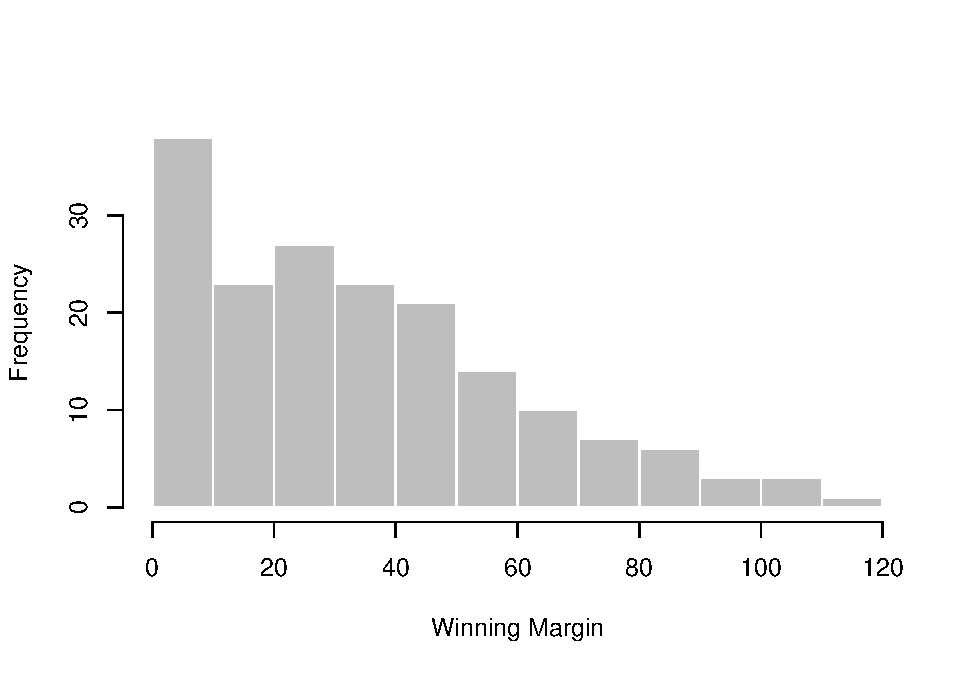
\includegraphics{navarro2_files/figure-latex/histogram1-1.pdf}
\caption{\label{fig:histogram1}A histogram of the AFL 2010 winning margin
data (the \texttt{afl.margins} variable). As you might expect, the
larger the margin the less frequently you tend to see it.}
\end{figure}

\section{Measures of central tendency}\label{centraltendency}

Drawing pictures of the data, as I did in Figure \ref{fig:histogram1} is
an excellent way to convey the ``gist'' of what the data is trying to
tell you, it's often extremely useful to try to condense the data into a
few simple ``summary'' statistics. In most situations, the first thing
that you'll want to calculate is a measure of \textbf{\emph{central
tendency}}. That is, you'd like to know something about the ``average''
or ``middle'' of your data lies. The two most commonly used measures are
the mean, median and mode; occasionally people will also report a
trimmed mean. I'll explain each of these in turn, and then discuss when
each of them is useful.

\subsection{The mean}\label{mean}

The \textbf{\emph{mean}} of a set of observations is just a normal,
old-fashioned average: add all of the values up, and then divide by the
total number of values. The first five AFL margins were 56, 31, 56, 8
and 32, so the mean of these observations is just: \[
\frac{56 + 31 + 56 + 8 + 32}{5} = \frac{183}{5} = 36.60
\] Of course, this definition of the mean isn't news to anyone: averages
(i.e., means) are used so often in everyday life that this is pretty
familiar stuff. However, since the concept of a mean is something that
everyone already understands, I'll use this as an excuse to start
introducing some of the mathematical notation that statisticians use to
describe this calculation, and talk about how the calculations would be
done in R.

The first piece of notation to introduce is \(N\), which we'll use to
refer to the number of observations that we're averaging (in this case
\(N = 5\)). Next, we need to attach a label to the observations
themselves. It's traditional to use \(X\) for this, and to use
subscripts to indicate which observation we're actually talking about.
That is, we'll use \(X_1\) to refer to the first observation, \(X_2\) to
refer to the second observation, and so on, all the way up to \(X_N\)
for the last one. Or, to say the same thing in a slightly more abstract
way, we use \(X_i\) to refer to the \(i\)-th observation. Just to make
sure we're clear on the notation, the following table lists the 5
observations in the \texttt{afl.margins} variable, along with the
mathematical symbol used to refer to it, and the actual value that the
observation corresponds to:

\begin{tabular}{lll}
\toprule
the observation & its symbol & the observed value\\
\midrule
winning margin, game 1 & \$X\_1\$ & 56 points\\
winning margin, game 2 & \$X\_2\$ & 31 points\\
winning margin, game 3 & \$X\_3\$ & 56 points\\
winning margin, game 4 & \$X\_4\$ & 8 points\\
winning margin, game 5 & \$X\_5\$ & 32 points\\
\bottomrule
\end{tabular}

Okay, now let's try to write a formula for the mean. By tradition, we
use \(\bar{X}\) as the notation for the mean. So the calculation for the
mean could be expressed using the following formula: \[
\bar{X} = \frac{X_1 + X_2 + ... + X_{N-1} + X_N}{N}
\] This formula is entirely correct, but it's terribly long, so we make
use of the \textbf{\emph{summation symbol}} \(\scriptstyle\sum\) to
shorten it.\footnote{The choice to use \(\Sigma\) to denote summation
  isn't arbitrary: it's the Greek upper case letter sigma, which is the
  analogue of the letter S in that alphabet. Similarly, there's an
  equivalent symbol used to denote the multiplication of lots of
  numbers: because multiplications are also called ``products'', we use
  the \(\Pi\) symbol for this; the Greek upper case pi, which is the
  analogue of the letter P.} If I want to add up the first five
observations, I could write out the sum the long way,
\(X_1 + X_2 + X_3 + X_4 +X_5\) or I could use the summation symbol to
shorten it to this: \[
\sum_{i=1}^5 X_i
\] Taken literally, this could be read as ``the sum, taken over all
\(i\) values from 1 to 5, of the value \(X_i\)''. But basically, what it
means is ``add up the first five observations''. In any case, we can use
this notation to write out the formula for the mean, which looks like
this: \[
\bar{X} = \frac{1}{N} \sum_{i=1}^N X_i 
\]

In all honesty, I can't imagine that all this mathematical notation
helps clarify the concept of the mean at all. In fact, it's really just
a fancy way of writing out the same thing I said in words: add all the
values up, and then divide by the total number of items. However, that's
not really the reason I went into all that detail. My goal was to try to
make sure that everyone reading this book is clear on the notation that
we'll be using throughout the book: \(\bar{X}\) for the mean,
\(\scriptstyle\sum\) for the idea of summation, \(X_i\) for the \(i\)th
observation, and \(N\) for the total number of observations. We're going
to be re-using these symbols a fair bit, so it's important that you
understand them well enough to be able to ``read'' the equations, and to
be able to see that it's just saying ``add up lots of things and then
divide by another thing''.

\subsection{Calculating the mean in R}\label{calculating-the-mean-in-r}

Okay that's the maths, how do we get the magic computing box to do the
work for us? If you really wanted to, you could do this calculation
directly in R. For the first 5 AFL scores, do this just by typing it in
as if R were a calculator\ldots{}

\begin{Shaded}
\begin{Highlighting}[]
\NormalTok{(}\DecValTok{56} \OperatorTok{+}\StringTok{ }\DecValTok{31} \OperatorTok{+}\StringTok{ }\DecValTok{56} \OperatorTok{+}\StringTok{ }\DecValTok{8} \OperatorTok{+}\StringTok{ }\DecValTok{32}\NormalTok{) }\OperatorTok{/}\StringTok{ }\DecValTok{5}
\end{Highlighting}
\end{Shaded}

\begin{verbatim}
## [1] 36.6
\end{verbatim}

\ldots{} in which case R outputs the answer 36.6, just as if it were a
calculator. However, that's not the only way to do the calculations, and
when the number of observations starts to become large, it's easily the
most tedious. Besides, in almost every real world scenario, you've
already got the actual numbers stored in a variable of some kind, just
like we have with the \texttt{afl.margins} variable. Under those
circumstances, what you want is a function that will just add up all the
values stored in a numeric vector. That's what the \texttt{sum()}
function does. If we want to add up all 176 winning margins in the data
set, we can do so using the following command:\footnote{Note that, just
  as we saw with the combine function \texttt{c()} and the remove
  function \texttt{rm()}, the \texttt{sum()} function has unnamed
  arguments. I'll talk about unnamed arguments later in Section
  \ref{dotsargument}, but for now let's just ignore this detail.}

\begin{Shaded}
\begin{Highlighting}[]
\KeywordTok{sum}\NormalTok{( afl.margins )}
\end{Highlighting}
\end{Shaded}

\begin{verbatim}
## [1] 6213
\end{verbatim}

If we only want the sum of the first five observations, then we can use
square brackets to pull out only the first five elements of the vector.
So the command would now be:

\begin{Shaded}
\begin{Highlighting}[]
\KeywordTok{sum}\NormalTok{( afl.margins[}\DecValTok{1}\OperatorTok{:}\DecValTok{5}\NormalTok{] )}
\end{Highlighting}
\end{Shaded}

\begin{verbatim}
## [1] 183
\end{verbatim}

To calculate the mean, we now tell R to divide the output of this
summation by five, so the command that we need to type now becomes the
following:

\begin{Shaded}
\begin{Highlighting}[]
\KeywordTok{sum}\NormalTok{( afl.margins[}\DecValTok{1}\OperatorTok{:}\DecValTok{5}\NormalTok{] ) }\OperatorTok{/}\StringTok{ }\DecValTok{5}
\end{Highlighting}
\end{Shaded}

\begin{verbatim}
## [1] 36.6
\end{verbatim}

Although it's pretty easy to calculate the mean using the \texttt{sum()}
function, we can do it in an even easier way, since R also provides us
with the \texttt{mean()} function. To calculate the mean for all 176
games, we would use the following command:

\begin{Shaded}
\begin{Highlighting}[]
\KeywordTok{mean}\NormalTok{( }\DataTypeTok{x =}\NormalTok{ afl.margins )}
\end{Highlighting}
\end{Shaded}

\begin{verbatim}
## [1] 35.30114
\end{verbatim}

However, since \texttt{x} is the first argument to the function, I could
have omitted the argument name. In any case, just to show you that
there's nothing funny going on, here's what we would do to calculate the
mean for the first five observations:

\begin{Shaded}
\begin{Highlighting}[]
\KeywordTok{mean}\NormalTok{( afl.margins[}\DecValTok{1}\OperatorTok{:}\DecValTok{5}\NormalTok{] )}
\end{Highlighting}
\end{Shaded}

\begin{verbatim}
## [1] 36.6
\end{verbatim}

As you can see, this gives exactly the same answers as the previous
calculations.

\subsection{The median}\label{median}

The second measure of central tendency that people use a lot is the
\textbf{\emph{median}}, and it's even easier to describe than the mean.
The median of a set of observations is just the middle value. As before
let's imagine we were interested only in the first 5 AFL winning
margins: 56, 31, 56, 8 and 32. To figure out the median, we sort these
numbers into ascending order: \[
8, 31, \mathbf{32}, 56, 56
\] From inspection, it's obvious that the median value of these 5
observations is 32, since that's the middle one in the sorted list (I've
put it in bold to make it even more obvious). Easy stuff. But what
should we do if we were interested in the first 6 games rather than the
first 5? Since the sixth game in the season had a winning margin of 14
points, our sorted list is now \[
8, 14, \mathbf{31}, \mathbf{32}, 56, 56
\] and there are \emph{two} middle numbers, 31 and 32. The median is
defined as the average of those two numbers, which is of course 31.5. As
before, it's very tedious to do this by hand when you've got lots of
numbers. To illustrate this, here's what happens when you use R to sort
all 176 winning margins. First, I'll use the \texttt{sort()} function
(discussed in Chapter \ref{datahandling}) to display the winning margins
in increasing numerical order:

\begin{Shaded}
\begin{Highlighting}[]
\KeywordTok{sort}\NormalTok{( }\DataTypeTok{x =}\NormalTok{ afl.margins )}
\end{Highlighting}
\end{Shaded}

\begin{verbatim}
##   [1]   0   0   1   1   1   1   2   2   3   3   3   3   3   3   3   3   4
##  [18]   4   5   6   7   7   8   8   8   8   8   9   9   9   9   9   9  10
##  [35]  10  10  10  10  11  11  11  12  12  12  13  14  14  15  16  16  16
##  [52]  16  18  19  19  19  19  19  20  20  20  21  21  22  22  22  23  23
##  [69]  23  24  24  25  25  26  26  26  26  27  27  28  28  29  29  29  29
##  [86]  29  29  30  31  32  32  33  35  35  35  35  36  36  36  36  36  36
## [103]  37  38  38  38  38  38  39  39  40  41  42  43  43  44  44  44  44
## [120]  44  47  47  47  48  48  48  49  49  50  50  50  50  52  52  53  53
## [137]  54  54  55  55  55  56  56  56  57  60  61  61  63  64  65  65  66
## [154]  67  68  70  71  71  72  73  75  75  76  81  82  82  83  84  89  94
## [171]  95  98 101 104 108 116
\end{verbatim}

The middle values are 30 and 31, so the median winning margin for 2010
was 30.5 points. In real life, of course, no-one actually calculates the
median by sorting the data and then looking for the middle value. In
real life, we use the median command:

\begin{Shaded}
\begin{Highlighting}[]
\KeywordTok{median}\NormalTok{( }\DataTypeTok{x =}\NormalTok{ afl.margins )}
\end{Highlighting}
\end{Shaded}

\begin{verbatim}
## [1] 30.5
\end{verbatim}

which outputs the median value of 30.5.

\subsection{Mean or median? What's the
difference?}\label{mean-or-median-whats-the-difference}

\begin{figure}
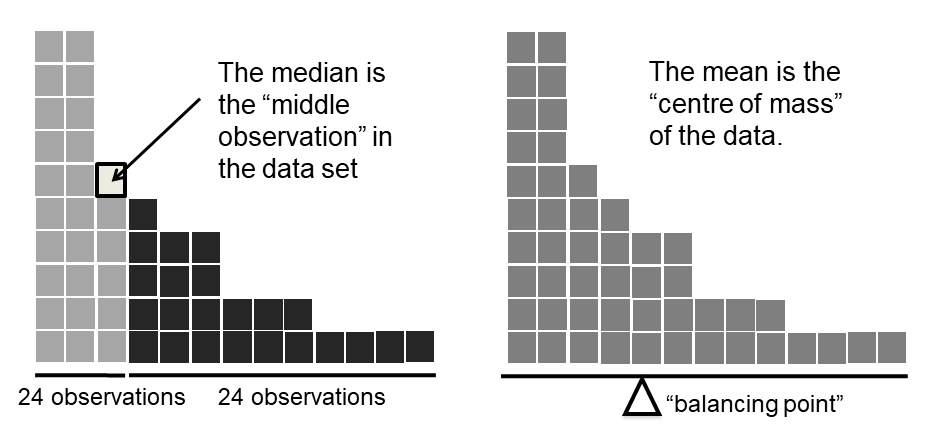
\includegraphics[width=12.86in]{./img/descriptives2/meanmedian} \caption{An illustration of the difference between how the mean and the median should be interpreted. The mean is basically the "centre of gravity" of the data set: if you imagine that the histogram of the data is a solid object, then the point on which you could balance it (as if on a see-saw) is the mean. In contrast, the median is the middle observation. Half of the observations are smaller, and half of the observations are larger.}\label{fig:meanmedian}
\end{figure}

Knowing how to calculate means and medians is only a part of the story.
You also need to understand what each one is saying about the data, and
what that implies for when you should use each one. This is illustrated
in Figure \ref{fig:meanmedian} the mean is kind of like the ``centre of
gravity'' of the data set, whereas the median is the ``middle value'' in
the data. What this implies, as far as which one you should use, depends
a little on what type of data you've got and what you're trying to
achieve. As a rough guide:

\begin{itemize}
\tightlist
\item
  If your data are nominal scale, you probably shouldn't be using either
  the mean or the median. Both the mean and the median rely on the idea
  that the numbers assigned to values are meaningful. If the numbering
  scheme is arbitrary, then it's probably best to use the mode (Section
  \ref{mode}) instead.
\item
  If your data are ordinal scale, you're more likely to want to use the
  median than the mean. The median only makes use of the order
  information in your data (i.e., which numbers are bigger), but doesn't
  depend on the precise numbers involved. That's exactly the situation
  that applies when your data are ordinal scale. The mean, on the other
  hand, makes use of the precise numeric values assigned to the
  observations, so it's not really appropriate for ordinal data.
\item
  For interval and ratio scale data, either one is generally acceptable.
  Which one you pick depends a bit on what you're trying to achieve. The
  mean has the advantage that it uses all the information in the data
  (which is useful when you don't have a lot of data), but it's very
  sensitive to extreme values, as we'll see in Section
  \ref{trimmedmean}.
\end{itemize}

Let's expand on that last part a little. One consequence is that there's
systematic differences between the mean and the median when the
histogram is asymmetric (skewed; see Section \ref{skewandkurtosis}).
This is illustrated in Figure \ref{fig:meanmedian} notice that the
median (right hand side) is located closer to the ``body'' of the
histogram, whereas the mean (left hand side) gets dragged towards the
``tail'' (where the extreme values are). To give a concrete example,
suppose Bob (income \$50,000), Kate (income \$60,000) and Jane (income
\$65,000) are sitting at a table: the average income at the table is
\$58,333 and the median income is \$60,000. Then Bill sits down with
them (income \$100,000,000). The average income has now jumped to
\$25,043,750 but the median rises only to \$62,500. If you're interested
in looking at the overall income at the table, the mean might be the
right answer; but if you're interested in what counts as a typical
income at the table, the median would be a better choice here.

\subsection{A real life example}\label{housingpriceexample}

To try to get a sense of why you need to pay attention to the
differences between the mean and the median, let's consider a real life
example. Since I tend to mock journalists for their poor scientific and
statistical knowledge, I should give credit where credit is due. This is
from an excellent article on the ABC news website\footnote{www.abc.net.au/news/stories/2010/09/24/3021480.htm}
24 September, 2010:

\begin{quote}
Senior Commonwealth Bank executives have travelled the world in the past
couple of weeks with a presentation showing how Australian house prices,
and the key price to income ratios, compare favourably with similar
countries. ``Housing affordability has actually been going sideways for
the last five to six years,'' said Craig James, the chief economist of
the bank's trading arm, CommSec.
\end{quote}

This probably comes as a huge surprise to anyone with a mortgage, or who
wants a mortgage, or pays rent, or isn't completely oblivious to what's
been going on in the Australian housing market over the last several
years. Back to the article:

\begin{quote}
CBA has waged its war against what it believes are housing doomsayers
with graphs, numbers and international comparisons. In its presentation,
the bank rejects arguments that Australia's housing is relatively
expensive compared to incomes. It says Australia's house price to
household income ratio of 5.6 in the major cities, and 4.3 nationwide,
is comparable to many other developed nations. It says San Francisco and
New York have ratios of 7, Auckland's is 6.7, and Vancouver comes in at
9.3.
\end{quote}

More excellent news! Except, the article goes on to make the observation
that\ldots{}

\begin{quote}
Many analysts say that has led the bank to use misleading figures and
comparisons. If you go to page four of CBA's presentation and read the
source information at the bottom of the graph and table, you would
notice there is an additional source on the international comparison --
Demographia. However, if the Commonwealth Bank had also used
Demographia's analysis of Australia's house price to income ratio, it
would have come up with a figure closer to 9 rather than 5.6 or 4.3
\end{quote}

That's, um, a rather serious discrepancy. One group of people say 9,
another says 4-5. Should we just split the difference, and say the truth
lies somewhere in between? Absolutely not: this is a situation where
there is a right answer and a wrong answer. Demographia are correct, and
the Commonwealth Bank is incorrect. As the article points out

\begin{quote}
{[}An{]} obvious problem with the Commonwealth Bank's domestic price to
income figures is they compare average incomes with median house prices
(unlike the Demographia figures that compare median incomes to median
prices). The median is the mid-point, effectively cutting out the highs
and lows, and that means the average is generally higher when it comes
to incomes and asset prices, because it includes the earnings of
Australia's wealthiest people. To put it another way: the Commonwealth
Bank's figures count Ralph Norris' multi-million dollar pay packet on
the income side, but not his (no doubt) very expensive house in the
property price figures, thus understating the house price to income
ratio for middle-income Australians.
\end{quote}

Couldn't have put it better myself. The way that Demographia calculated
the ratio is the right thing to do. The way that the Bank did it is
incorrect. As for why an extremely quantitatively sophisticated
organisation such as a major bank made such an elementary mistake,
well\ldots{} I can't say for sure, since I have no special insight into
their thinking, but the article itself does happen to mention the
following facts, which may or may not be relevant:

\begin{quote}
{[}As{]} Australia's largest home lender, the Commonwealth Bank has one
of the biggest vested interests in house prices rising. It effectively
owns a massive swathe of Australian housing as security for its home
loans as well as many small business loans.
\end{quote}

My, my.

\subsection{Trimmed mean}\label{trimmedmean}

One of the fundamental rules of applied statistics is that the data are
messy. Real life is never simple, and so the data sets that you obtain
are never as straightforward as the statistical theory says.\footnote{Or
  at least, the basic statistical theory -- these days there is a whole
  subfield of statistics called \emph{robust statistics} that tries to
  grapple with the messiness of real data and develop theory that can
  cope with it.} This can have awkward consequences. To illustrate,
consider this rather strange looking data set: \[
-100,2,3,4,5,6,7,8,9,10
\] If you were to observe this in a real life data set, you'd probably
suspect that something funny was going on with the \(-100\) value. It's
probably an \textbf{\emph{outlier}}, a value that doesn't really belong
with the others. You might consider removing it from the data set
entirely, and in this particular case I'd probably agree with that
course of action. In real life, however, you don't always get such
cut-and-dried examples. For instance, you might get this instead: \[
-15,2,3,4,5,6,7,8,9,12
\] The \(-15\) looks a bit suspicious, but not anywhere near as much as
that \(-100\) did. In this case, it's a little trickier. It \emph{might}
be a legitimate observation, it might not.

When faced with a situation where some of the most extreme-valued
observations might not be quite trustworthy, the mean is not necessarily
a good measure of central tendency. It is highly sensitive to one or two
extreme values, and is thus not considered to be a
\textbf{\emph{robust}} measure. One remedy that we've seen is to use the
median. A more general solution is to use a ``trimmed mean''. To
calculate a trimmed mean, what you do is ``discard'' the most extreme
examples on both ends (i.e., the largest and the smallest), and then
take the mean of everything else. The goal is to preserve the best
characteristics of the mean and the median: just like a median, you
aren't highly influenced by extreme outliers, but like the mean, you
``use'' more than one of the observations. Generally, we describe a
trimmed mean in terms of the percentage of observation on either side
that are discarded. So, for instance, a 10\% trimmed mean discards the
largest 10\% of the observations \emph{and} the smallest 10\% of the
observations, and then takes the mean of the remaining 80\% of the
observations. Not surprisingly, the 0\% trimmed mean is just the regular
mean, and the 50\% trimmed mean is the median. In that sense, trimmed
means provide a whole family of central tendency measures that span the
range from the mean to the median.

For our toy example above, we have 10 observations, and so a 10\%
trimmed mean is calculated by ignoring the largest value (i.e.,
\texttt{12}) and the smallest value (i.e., \texttt{-15}) and taking the
mean of the remaining values. First, let's enter the data

\begin{Shaded}
\begin{Highlighting}[]
\NormalTok{dataset <-}\StringTok{ }\KeywordTok{c}\NormalTok{( }\OperatorTok{-}\DecValTok{15}\NormalTok{,}\DecValTok{2}\NormalTok{,}\DecValTok{3}\NormalTok{,}\DecValTok{4}\NormalTok{,}\DecValTok{5}\NormalTok{,}\DecValTok{6}\NormalTok{,}\DecValTok{7}\NormalTok{,}\DecValTok{8}\NormalTok{,}\DecValTok{9}\NormalTok{,}\DecValTok{12}\NormalTok{ )}
\end{Highlighting}
\end{Shaded}

Next, let's calculate means and medians:

\begin{Shaded}
\begin{Highlighting}[]
\KeywordTok{mean}\NormalTok{( }\DataTypeTok{x =}\NormalTok{ dataset )}
\end{Highlighting}
\end{Shaded}

\begin{verbatim}
## [1] 4.1
\end{verbatim}

\begin{Shaded}
\begin{Highlighting}[]
\KeywordTok{median}\NormalTok{( }\DataTypeTok{x =}\NormalTok{ dataset )}
\end{Highlighting}
\end{Shaded}

\begin{verbatim}
## [1] 5.5
\end{verbatim}

That's a fairly substantial difference, but I'm tempted to think that
the mean is being influenced a bit too much by the extreme values at
either end of the data set, especially the \(-15\) one. So let's just
try trimming the mean a bit. If I take a 10\% trimmed mean, we'll drop
the extreme values on either side, and take the mean of the rest:

\begin{Shaded}
\begin{Highlighting}[]
\KeywordTok{mean}\NormalTok{( }\DataTypeTok{x =}\NormalTok{ dataset, }\DataTypeTok{trim =}\NormalTok{ .}\DecValTok{1}\NormalTok{)}
\end{Highlighting}
\end{Shaded}

\begin{verbatim}
## [1] 5.5
\end{verbatim}

which in this case gives exactly the same answer as the median. Note
that, to get a 10\% trimmed mean you write \texttt{trim\ =\ .1}, not
\texttt{trim\ =\ 10}. In any case, let's finish up by calculating the
5\% trimmed mean for the \texttt{afl.margins} data,

\begin{Shaded}
\begin{Highlighting}[]
\KeywordTok{mean}\NormalTok{( }\DataTypeTok{x =}\NormalTok{ afl.margins, }\DataTypeTok{trim =}\NormalTok{ .}\DecValTok{05}\NormalTok{)  }
\end{Highlighting}
\end{Shaded}

\begin{verbatim}
## [1] 33.75
\end{verbatim}

\subsection{Mode}\label{mode}

The mode of a sample is very simple: it is the value that occurs most
frequently. To illustrate the mode using the AFL data, let's examine a
different aspect to the data set. Who has played in the most finals? The
\texttt{afl.finalists} variable is a factor that contains the name of
every team that played in any AFL final from 1987-2010, so let's have a
look at it. To do this we will use the \texttt{head()} command.
\texttt{head()} is useful when you're working with a data.frame with a
lot of rows since you can use it to tell you how many rows to return.
There have been a lot of finals in this period so printing afl.finalists
using \texttt{print(afl.finalists)} will just fill us the screen. The
command below tells R we just want the first 25 rows of the data.frame.

\begin{Shaded}
\begin{Highlighting}[]
\KeywordTok{head}\NormalTok{(afl.finalists, }\DecValTok{25}\NormalTok{)}
\end{Highlighting}
\end{Shaded}

\begin{verbatim}
##  [1] Hawthorn    Melbourne   Carlton     Melbourne   Hawthorn   
##  [6] Carlton     Melbourne   Carlton     Hawthorn    Melbourne  
## [11] Melbourne   Hawthorn    Melbourne   Essendon    Hawthorn   
## [16] Geelong     Geelong     Hawthorn    Collingwood Melbourne  
## [21] Collingwood West Coast  Collingwood Essendon    Collingwood
## 17 Levels: Adelaide Brisbane Carlton Collingwood Essendon ... Western Bulldogs
\end{verbatim}

There are actually 400 entries (aren't you glad we didn't print them
all?). We \emph{could} read through all 400, and count the number of
occasions on which each team name appears in our list of finalists,
thereby producing a \textbf{\emph{frequency table}}. However, that would
be mindless and boring: exactly the sort of task that computers are
great at. So let's use the \texttt{table()} function (discussed in more
detail in Section \ref{freqtables}) to do this task for us:

\begin{Shaded}
\begin{Highlighting}[]
\KeywordTok{table}\NormalTok{( afl.finalists )}
\end{Highlighting}
\end{Shaded}

\begin{verbatim}
## afl.finalists
##         Adelaide         Brisbane          Carlton      Collingwood 
##               26               25               26               28 
##         Essendon          Fitzroy        Fremantle          Geelong 
##               32                0                6               39 
##         Hawthorn        Melbourne  North Melbourne    Port Adelaide 
##               27               28               28               17 
##         Richmond         St Kilda           Sydney       West Coast 
##                6               24               26               38 
## Western Bulldogs 
##               24
\end{verbatim}

Now that we have our frequency table, we can just look at it and see
that, over the 24 years for which we have data, Geelong has played in
more finals than any other team. Thus, the mode of the
\texttt{finalists} data is \texttt{"Geelong"}. The core packages in R
don't have a function for calculating the mode\footnote{As we saw
  earlier, it \emph{does} have a function called \texttt{mode()}, but it
  does something completely different.}. However, I've included a
function in the \texttt{lsr} package that does this. The function is
called \texttt{modeOf()}, and here's how you use it:

\begin{Shaded}
\begin{Highlighting}[]
\KeywordTok{modeOf}\NormalTok{( }\DataTypeTok{x =}\NormalTok{ afl.finalists )}
\end{Highlighting}
\end{Shaded}

\begin{verbatim}
## [1] "Geelong"
\end{verbatim}

There's also a function called \texttt{maxFreq()} that tells you what
the modal frequency is. If we apply this function to our finalists data,
we obtain the following:

\begin{Shaded}
\begin{Highlighting}[]
\KeywordTok{maxFreq}\NormalTok{( }\DataTypeTok{x =}\NormalTok{ afl.finalists )}
\end{Highlighting}
\end{Shaded}

\begin{verbatim}
## [1] 39
\end{verbatim}

Taken together, we observe that Geelong (39 finals) played in more
finals than any other team during the 1987-2010 period.

One last point to make with respect to the mode. While it's generally
true that the mode is most often calculated when you have nominal scale
data (because means and medians are useless for those sorts of
variables), there are some situations in which you really do want to
know the mode of an ordinal, interval or ratio scale variable. For
instance, let's go back to thinking about our \texttt{afl.margins}
variable. This variable is clearly ratio scale (if it's not clear to
you, it may help to re-read Section \ref{scales}), and so in most
situations the mean or the median is the measure of central tendency
that you want. But consider this scenario\ldots{} a friend of yours is
offering a bet. They pick a football game at random, and (without
knowing who is playing) you have to guess the \emph{exact} margin. If
you guess correctly, you win \$50. If you don't, you lose \$1. There are
no consolation prizes for ``almost'' getting the right answer. You have
to guess exactly the right margin\footnote{This is called a ``0-1 loss
  function'', meaning that you either win (1) or you lose (0), with no
  middle ground.} For this bet, the mean and the median are completely
useless to you. It is the mode that you should bet on. So, we calculate
this modal value

\begin{Shaded}
\begin{Highlighting}[]
\KeywordTok{modeOf}\NormalTok{( }\DataTypeTok{x =}\NormalTok{ afl.margins )}
\end{Highlighting}
\end{Shaded}

\begin{verbatim}
## [1] 3
\end{verbatim}

\begin{Shaded}
\begin{Highlighting}[]
\KeywordTok{maxFreq}\NormalTok{( }\DataTypeTok{x =}\NormalTok{ afl.margins )}
\end{Highlighting}
\end{Shaded}

\begin{verbatim}
## [1] 8
\end{verbatim}

So the 2010 data suggest you should bet on a 3 point margin, and since
this was observed in 8 of the 176 game (4.5\% of games) the odds are
firmly in your favour.

\section{Measures of variability}\label{var}

The statistics that we've discussed so far all relate to \emph{central
tendency}. That is, they all talk about which values are ``in the
middle'' or ``popular'' in the data. However, central tendency is not
the only type of summary statistic that we want to calculate. The second
thing that we really want is a measure of the
\textbf{\emph{variability}} of the data. That is, how ``spread out'' are
the data? How ``far'' away from the mean or median do the observed
values tend to be? For now, let's assume that the data are interval or
ratio scale, so we'll continue to use the \texttt{afl.margins} data.
We'll use this data to discuss several different measures of spread,
each with different strengths and weaknesses.

\subsection{Range}\label{range}

The \textbf{\emph{range}} of a variable is very simple: it's the biggest
value minus the smallest value. For the AFL winning margins data, the
maximum value is 116, and the minimum value is 0. We can calculate these
values in R using the \texttt{max()} and \texttt{min()} functions:

\begin{Shaded}
\begin{Highlighting}[]
\KeywordTok{max}\NormalTok{( afl.margins )}
\end{Highlighting}
\end{Shaded}

\begin{verbatim}
## [1] 116
\end{verbatim}

\begin{Shaded}
\begin{Highlighting}[]
\KeywordTok{min}\NormalTok{( afl.margins )}
\end{Highlighting}
\end{Shaded}

\begin{verbatim}
## [1] 0
\end{verbatim}

where I've omitted the output because it's not interesting. The other
possibility is to use the \texttt{range()} function; which outputs both
the minimum value and the maximum value in a vector, like this:

\begin{Shaded}
\begin{Highlighting}[]
\KeywordTok{range}\NormalTok{( afl.margins )}
\end{Highlighting}
\end{Shaded}

\begin{verbatim}
## [1]   0 116
\end{verbatim}

Although the range is the simplest way to quantify the notion of
``variability'', it's one of the worst. Recall from our discussion of
the mean that we want our summary measure to be robust. If the data set
has one or two extremely bad values in it, we'd like our statistics not
to be unduly influenced by these cases. If we look once again at our toy
example of a data set containing very extreme outliers\ldots{} \[
-100,2,3,4,5,6,7,8,9,10
\] \ldots{} it is clear that the range is not robust, since this has a
range of 110, but if the outlier were removed we would have a range of
only 8.

\subsection{Interquartile range}\label{interquartile-range}

The \textbf{\emph{interquartile range}} (IQR) is like the range, but
instead of calculating the difference between the biggest and smallest
value, it calculates the difference between the 25th quantile and the
75th quantile. Probably you already know what a \textbf{\emph{quantile}}
is (they're more commonly called percentiles), but if not: the 10th
percentile of a data set is the smallest number \(x\) such that 10\% of
the data is less than \(x\). In fact, we've already come across the
idea: the median of a data set is its 50th quantile / percentile! R
actually provides you with a way of calculating quantiles, using the
(surprise, surprise) \texttt{quantile()} function. Let's use it to
calculate the median AFL winning margin:

\begin{Shaded}
\begin{Highlighting}[]
\KeywordTok{quantile}\NormalTok{( }\DataTypeTok{x =}\NormalTok{ afl.margins, }\DataTypeTok{probs =}\NormalTok{ .}\DecValTok{5}\NormalTok{)}
\end{Highlighting}
\end{Shaded}

\begin{verbatim}
##  50% 
## 30.5
\end{verbatim}

And not surprisingly, this agrees with the answer that we saw earlier
with the \texttt{median()} function. Now, we can actually input lots of
quantiles at once, by specifying a vector for the \texttt{probs}
argument. So lets do that, and get the 25th and 75th percentile:

\begin{Shaded}
\begin{Highlighting}[]
\KeywordTok{quantile}\NormalTok{( }\DataTypeTok{x =}\NormalTok{ afl.margins, }\DataTypeTok{probs =} \KeywordTok{c}\NormalTok{(.}\DecValTok{25}\NormalTok{,.}\DecValTok{75}\NormalTok{) )}
\end{Highlighting}
\end{Shaded}

\begin{verbatim}
##   25%   75% 
## 12.75 50.50
\end{verbatim}

And, by noting that \(50.5 - 12.75 = 37.75\), we can see that the
interquartile range for the 2010 AFL winning margins data is 37.75. Of
course, that seems like too much work to do all that typing, so R has a
built in function called \texttt{IQR()} that we can use:

\begin{Shaded}
\begin{Highlighting}[]
\KeywordTok{IQR}\NormalTok{( }\DataTypeTok{x =}\NormalTok{ afl.margins )}
\end{Highlighting}
\end{Shaded}

\begin{verbatim}
## [1] 37.75
\end{verbatim}

While it's obvious how to interpret the range, it's a little less
obvious how to interpret the IQR. The simplest way to think about it is
like this: the interquartile range is the range spanned by the ``middle
half'' of the data. That is, one quarter of the data falls below the
25th percentile, one quarter of the data is above the 75th percentile,
leaving the ``middle half'' of the data lying in between the two. And
the IQR is the range covered by that middle half.

\subsection{Mean absolute deviation}\label{aad}

The two measures we've looked at so far, the range and the interquartile
range, both rely on the idea that we can measure the spread of the data
by looking at the quantiles of the data. However, this isn't the only
way to think about the problem. A different approach is to select a
meaningful reference point (usually the mean or the median) and then
report the ``typical'' deviations from that reference point. What do we
mean by ``typical'' deviation? Usually, the mean or median value of
these deviations! In practice, this leads to two different measures, the
``mean absolute deviation (from the mean)'' and the ``median absolute
deviation (from the median)''. From what I've read, the measure based on
the median seems to be used in statistics, and does seem to be the
better of the two, but to be honest I don't think I've seen it used much
in psychology. The measure based on the mean does occasionally show up
in psychology though. In this section I'll talk about the first one, and
I'll come back to talk about the second one later.

Since the previous paragraph might sound a little abstract, let's go
through the \textbf{\emph{mean absolute deviation}} from the mean a
little more slowly. One useful thing about this measure is that the name
actually tells you exactly how to calculate it. Let's think about our
AFL winning margins data, and once again we'll start by pretending that
there's only 5 games in total, with winning margins of 56, 31, 56, 8 and
32. Since our calculations rely on an examination of the deviation from
some reference point (in this case the mean), the first thing we need to
calculate is the mean, \(\bar{X}\). For these five observations, our
mean is \(\bar{X} = 36.6\). The next step is to convert each of our
observations \(X_i\) into a deviation score. We do this by calculating
the difference between the observation \(X_i\) and the mean \(\bar{X}\).
That is, the deviation score is defined to be \(X_i - \bar{X}\). For the
first observation in our sample, this is equal to \(56 - 36.6 = 19.4\).
Okay, that's simple enough. The next step in the process is to convert
these deviations to absolute deviations. As we discussed earlier when
talking about the \texttt{abs()} function in R (Section
\ref{usingfunctions}), we do this by converting any negative values to
positive ones. Mathematically, we would denote the absolute value of
\(-3\) as \(|-3|\), and so we say that \(|-3| = 3\). We use the absolute
value function here because we don't really care whether the value is
higher than the mean or lower than the mean, we're just interested in
how \emph{close} it is to the mean. To help make this process as obvious
as possible, the table below shows these calculations for all five
observations:

\begin{tabular}{lll}
\toprule
the observation & its symbol & the observed value\\
\midrule
winning margin, game 1 & \$X\_1\$ & 56 points\\
winning margin, game 2 & \$X\_2\$ & 31 points\\
winning margin, game 3 & \$X\_3\$ & 56 points\\
winning margin, game 4 & \$X\_4\$ & 8 points\\
winning margin, game 5 & \$X\_5\$ & 32 points\\
\bottomrule
\end{tabular}

Now that we have calculated the absolute deviation score for every
observation in the data set, all that we have to do to calculate the
mean of these scores. Let's do that: \[
\frac{19.4 + 5.6 + 19.4 + 28.6 + 4.6}{5} = 15.52
\] And we're done. The mean absolute deviation for these five scores is
15.52.

However, while our calculations for this little example are at an end,
we do have a couple of things left to talk about. Firstly, we should
really try to write down a proper mathematical formula. But in order do
to this I need some mathematical notation to refer to the mean absolute
deviation. Irritatingly, ``mean absolute deviation'' and ``median
absolute deviation'' have the same acronym (MAD), which leads to a
certain amount of ambiguity, and since R tends to use MAD to refer to
the median absolute deviation, I'd better come up with something
different for the mean absolute deviation. Sigh. What I'll do is use AAD
instead, short for \emph{average} absolute deviation. Now that we have
some unambiguous notation, here's the formula that describes what we
just calculated: \[
\mbox{}(X) = \frac{1}{N} \sum_{i = 1}^N |X_i - \bar{X}|
\]

The last thing we need to talk about is how to calculate AAD in R. One
possibility would be to do everything using low level commands,
laboriously following the same steps that I used when describing the
calculations above. However, that's pretty tedious. You'd end up with a
series of commands that might look like this:

\begin{Shaded}
\begin{Highlighting}[]
\NormalTok{X <-}\StringTok{ }\KeywordTok{c}\NormalTok{(}\DecValTok{56}\NormalTok{, }\DecValTok{31}\NormalTok{,}\DecValTok{56}\NormalTok{,}\DecValTok{8}\NormalTok{,}\DecValTok{32}\NormalTok{)   }\CommentTok{# enter the data}
\NormalTok{X.bar <-}\StringTok{ }\KeywordTok{mean}\NormalTok{( X )       }\CommentTok{# step 1. the mean of the data}
\NormalTok{AD <-}\StringTok{ }\KeywordTok{abs}\NormalTok{( X }\OperatorTok{-}\StringTok{ }\NormalTok{X.bar )   }\CommentTok{# step 2. the absolute deviations from the mean}
\NormalTok{AAD <-}\StringTok{ }\KeywordTok{mean}\NormalTok{( AD )        }\CommentTok{# step 3. the mean absolute deviations}
\KeywordTok{print}\NormalTok{( AAD )             }\CommentTok{# print the results}
\end{Highlighting}
\end{Shaded}

\begin{verbatim}
## [1] 15.52
\end{verbatim}

Each of those commands is pretty simple, but there's just too many of
them. And because I find that to be too much typing, the \texttt{lsr}
package has a very simple function called \texttt{aad()} that does the
calculations for you. If we apply the \texttt{aad()} function to our
data, we get this:

\begin{Shaded}
\begin{Highlighting}[]
\KeywordTok{library}\NormalTok{(lsr)}
\KeywordTok{aad}\NormalTok{( X )}
\end{Highlighting}
\end{Shaded}

\begin{verbatim}
## [1] 15.52
\end{verbatim}

No suprises there.

\subsection{Variance}\label{variance}

Although the mean absolute deviation measure has its uses, it's not the
best measure of variability to use. From a purely mathematical
perspective, there are some solid reasons to prefer squared deviations
rather than absolute deviations. If we do that, we obtain a measure is
called the \textbf{\emph{variance}}, which has a lot of really nice
statistical properties that I'm going to ignore,\footnote{Well, I will
  very briefly mention the one that I think is coolest, for a very
  particular definition of ``cool'', that is. Variances are
  \emph{additive}. Here's what that means: suppose I have two variables
  \(X\) and \(Y\), whose variances are \$\mbox{Var}}(X)\$ and
\(\mbox{Var}(Y)\) respectively. Now imagine I want to define a new
variable \(Z\) that is the sum of the two, \(Z = X+Y\). As it turns out,
the variance of \(Z\) is equal to \(\mbox{Var}(X) + \mbox{Var}(Y)\).
This is a \emph{very} useful property, but it's not true of the other
measures that I talk about in this section.{]} and one massive
psychological flaw that I'm going to make a big deal out of in a moment.
The variance of a data set \(X\) is sometimes written as
\(\mbox{Var}(X)\), but it's more commonly denoted \(s^2\) (the reason
for this will become clearer shortly). The formula that we use to
calculate the variance of a set of observations is as follows: \[
\mbox{Var}(X) = \frac{1}{N} \sum_{i=1}^N \left( X_i - \bar{X} \right)^2
\]
\[\mbox{Var}(X) = \frac{\sum_{i=1}^N \left( X_i - \bar{X} \right)^2}{N}\]
As you can see, it's basically the same formula that we used to
calculate the mean absolute deviation, except that instead of using
``absolute deviations'' we use ``squared deviations''. It is for this
reason that the variance is sometimes referred to as the ``mean square
deviation''.

Now that we've got the basic idea, let's have a look at a concrete
example. Once again, let's use the first five AFL games as our data. If
we follow the same approach that we took last time, we end up with the
following table:

\begin{table}

\caption{\label{tab:unnamed-chunk-187}Basic arithmetic operations in R. These five operators are used very frequently throughout the text, so it's important to be familiar with them at the outset.}
\centering
\begin{tabular}[t]{lllll}
\toprule
Notation [English] & \$i\$ [which game] & \$X\_i\$ [value] & \$X\_i - \textbackslash{}bar\{X\}\$ [deviation from mean] & \$(X\_i - \textbackslash{}bar\{X\})\textasciicircum{}2\$ [absolute deviation]\\
\midrule
 & 1 & 56 & 19.4 & 376.36\\
 & 2 & 31 & -5.6 & 31.36\\
 & 3 & 56 & 19.4 & 376.36\\
 & 4 & 8 & -28.6 & 817.96\\
 & 5 & 32 & -4.6 & 21.16\\
\bottomrule
\end{tabular}
\end{table}

That last column contains all of our squared deviations, so all we have
to do is average them. If we do that by typing all the numbers into R by
hand\ldots{}

\begin{Shaded}
\begin{Highlighting}[]
\NormalTok{( }\FloatTok{376.36} \OperatorTok{+}\StringTok{ }\FloatTok{31.36} \OperatorTok{+}\StringTok{ }\FloatTok{376.36} \OperatorTok{+}\StringTok{ }\FloatTok{817.96} \OperatorTok{+}\StringTok{ }\FloatTok{21.16}\NormalTok{ ) }\OperatorTok{/}\StringTok{ }\DecValTok{5}
\end{Highlighting}
\end{Shaded}

\begin{verbatim}
## [1] 324.64
\end{verbatim}

\ldots{} we end up with a variance of 324.64. Exciting, isn't it? For
the moment, let's ignore the burning question that you're all probably
thinking (i.e., what the heck does a variance of 324.64 actually mean?)
and instead talk a bit more about how to do the calculations in R,
because this will reveal something very weird.

As always, we want to avoid having to type in a whole lot of numbers
ourselves. And as it happens, we have the vector \texttt{X} lying
around, which we created in the previous section. With this in mind, we
can calculate the variance of \texttt{X} by using the following command,

\begin{Shaded}
\begin{Highlighting}[]
\KeywordTok{mean}\NormalTok{( (X }\OperatorTok{-}\StringTok{ }\KeywordTok{mean}\NormalTok{(X) )}\OperatorTok{^}\DecValTok{2}\NormalTok{)}
\end{Highlighting}
\end{Shaded}

\begin{verbatim}
## [1] 324.64
\end{verbatim}

and as usual we get the same answer as the one that we got when we did
everything by hand. However, I \emph{still} think that this is too much
typing. Fortunately, R has a built in function called \texttt{var()}
which does calculate variances. So we could also do this\ldots{}

\begin{Shaded}
\begin{Highlighting}[]
\KeywordTok{var}\NormalTok{(X)}
\end{Highlighting}
\end{Shaded}

\begin{verbatim}
## [1] 405.8
\end{verbatim}

and you get the same\ldots{} no, wait\ldots{} you get a completely
\emph{different} answer. That's just weird. Is R broken? Is this a typo?
Is Dan an idiot?

As it happens, the answer is no.\footnote{With the possible exception of
  the third question.} It's not a typo, and R is not making a mistake.
To get a feel for what's happening, let's stop using the tiny data set
containing only 5 data points, and switch to the full set of 176 games
that we've got stored in our \texttt{afl.margins} vector. First, let's
calculate the variance by using the formula that I described above:

\begin{Shaded}
\begin{Highlighting}[]
\KeywordTok{mean}\NormalTok{( (afl.margins }\OperatorTok{-}\StringTok{ }\KeywordTok{mean}\NormalTok{(afl.margins) )}\OperatorTok{^}\DecValTok{2}\NormalTok{)}
\end{Highlighting}
\end{Shaded}

\begin{verbatim}
## [1] 675.9718
\end{verbatim}

Now let's use the \texttt{var()} function:

\begin{Shaded}
\begin{Highlighting}[]
\KeywordTok{var}\NormalTok{( afl.margins )}
\end{Highlighting}
\end{Shaded}

\begin{verbatim}
## [1] 679.8345
\end{verbatim}

Hm. These two numbers are very similar this time. That seems like too
much of a coincidence to be a mistake. And of course it isn't a mistake.
In fact, it's very simple to explain what R is doing here, but slightly
trickier to explain \emph{why} R is doing it. So let's start with the
``what''. What R is doing is evaluating a slightly different formula to
the one I showed you above. Instead of averaging the squared deviations,
which requires you to divide by the number of data points \(N\), R has
chosen to divide by \(N-1\). In other words, the formula that R is using
is this one\\
\[
\frac{1}{N-1} \sum_{i=1}^N \left( X_i - \bar{X} \right)^2
\] It's easy enough to verify that this is what's happening, as the
following command illustrates:

\begin{Shaded}
\begin{Highlighting}[]
\KeywordTok{sum}\NormalTok{( (X}\OperatorTok{-}\KeywordTok{mean}\NormalTok{(X))}\OperatorTok{^}\DecValTok{2}\NormalTok{ ) }\OperatorTok{/}\StringTok{ }\DecValTok{4}
\end{Highlighting}
\end{Shaded}

\begin{verbatim}
## [1] 405.8
\end{verbatim}

This is the same answer that R gave us originally when we calculated
\texttt{var(X)} originally. So that's the \emph{what}. The real question
is \emph{why} R is dividing by \(N-1\) and not by \(N\). After all, the
variance is supposed to be the \emph{mean} squared deviation, right? So
shouldn't we be dividing by \(N\), the actual number of observations in
the sample? Well, yes, we should. However, as we'll discuss in Chapter
\ref{estimation}, there's a subtle distinction between ``describing a
sample'' and ``making guesses about the population from which the sample
came''. Up to this point, it's been a distinction without a difference.
Regardless of whether you're describing a sample or drawing inferences
about the population, the mean is calculated exactly the same way. Not
so for the variance, or the standard deviation, or for many other
measures besides. What I outlined to you initially (i.e., take the
actual average, and thus divide by \(N\)) assumes that you literally
intend to calculate the variance of the sample. Most of the time,
however, you're not terribly interested in the sample \emph{in and of
itself}. Rather, the sample exists to tell you something about the
world. If so, you're actually starting to move away from calculating a
``sample statistic'', and towards the idea of estimating a ``population
parameter''. However, I'm getting ahead of myself. For now, let's just
take it on faith that R knows what it's doing, and we'll revisit the
question later on when we talk about estimation in Chapter
\ref{estimation}.

Okay, one last thing. This section so far has read a bit like a mystery
novel. I've shown you how to calculate the variance, described the weird
``\(N-1\)'' thing that R does and hinted at the reason why it's there,
but I haven't mentioned the single most important thing\ldots{} how do
you \emph{interpret} the variance? Descriptive statistics are supposed
to describe things, after all, and right now the variance is really just
a gibberish number. Unfortunately, the reason why I haven't given you
the human-friendly interpretation of the variance is that there really
isn't one. This is the most serious problem with the variance. Although
it has some elegant mathematical properties that suggest that it really
is a fundamental quantity for expressing variation, it's completely
useless if you want to communicate with an actual human\ldots{}
variances are completely uninterpretable in terms of the original
variable! All the numbers have been squared, and they don't mean
anything anymore. This is a huge issue. For instance, according to the
table I presented earlier, the margin in game 1 was ``376.36
points-squared higher than the average margin''. This is \emph{exactly}
as stupid as it sounds; and so when we calculate a variance of 324.64,
we're in the same situation. I've watched a lot of footy games, and
never has anyone referred to ``points squared''. It's \emph{not} a real
unit of measurement, and since the variance is expressed in terms of
this gibberish unit, it is totally meaningless to a human.

\subsection{Standard deviation}\label{sd}

Okay, suppose that you like the idea of using the variance because of
those nice mathematical properties that I haven't talked about, but --
since you're a human and not a robot -- you'd like to have a measure
that is expressed in the same units as the data itself (i.e., points,
not points-squared). What should you do? The solution to the problem is
obvious: take the square root of the variance, known as the
\textbf{\emph{standard deviation}}, also called the ``root mean squared
deviation'', or RMSD. This solves out problem fairly neatly: while
nobody has a clue what ``a variance of 324.68 points-squared'' really
means, it's much easier to understand ``a standard deviation of 18.01
points'', since it's expressed in the original units. It is traditional
to refer to the standard deviation of a sample of data as \(s\), though
``sd'' and ``std dev.'' are also used at times. Because the standard
deviation is equal to the square root of the variance, you probably
won't be surprised to see that the formula is: \[
s = \sqrt{ \frac{1}{N} \sum_{i=1}^N \left( X_i - \bar{X} \right)^2 }
\] and the R function that we use to calculate it is \texttt{sd()}.
However, as you might have guessed from our discussion of the variance,
what R actually calculates is slightly different to the formula given
above. Just like the we saw with the variance, what R calculates is a
version that divides by \(N-1\) rather than \(N\). For reasons that will
make sense when we return to this topic in
\href{mailto:Chapter@refch}{\nolinkurl{Chapter@refch}}:estimation I'll
refer to this new quantity as \(\hat\sigma\) (read as: ``sigma hat''),
and the formula for this is \[
\hat\sigma = \sqrt{ \frac{1}{N-1} \sum_{i=1}^N \left( X_i - \bar{X} \right)^2 }
\] With that in mind, calculating standard deviations in R is simple:

\begin{Shaded}
\begin{Highlighting}[]
\KeywordTok{sd}\NormalTok{( afl.margins ) }
\end{Highlighting}
\end{Shaded}

\begin{verbatim}
## [1] 26.07364
\end{verbatim}

Interpreting standard deviations is slightly more complex. Because the
standard deviation is derived from the variance, and the variance is a
quantity that has little to no meaning that makes sense to us humans,
the standard deviation doesn't have a simple interpretation. As a
consequence, most of us just rely on a simple rule of thumb: in general,
you should expect 68\% of the data to fall within 1 standard deviation
of the mean, 95\% of the data to fall within 2 standard deviation of the
mean, and 99.7\% of the data to fall within 3 standard deviations of the
mean. This rule tends to work pretty well most of the time, but it's not
exact: it's actually calculated based on an \emph{assumption} that the
histogram is symmetric and ``bell shaped''.\footnote{Strictly, the
  assumption is that the data are \emph{normally} distributed, which is
  an important concept that we'll discuss more in Chapter
  \ref{probability}, and will turn up over and over again later in the
  book.} As you can tell from looking at the AFL winning margins
histogram in Figure \ref{fig:histogram1}, this isn't exactly true of our
data! Even so, the rule is approximately correct. As it turns out,
65.3\% of the AFL margins data fall within one standard deviation of the
mean. This is shown visually in Figure \ref{fig:aflsd}.

\begin{figure}
\centering
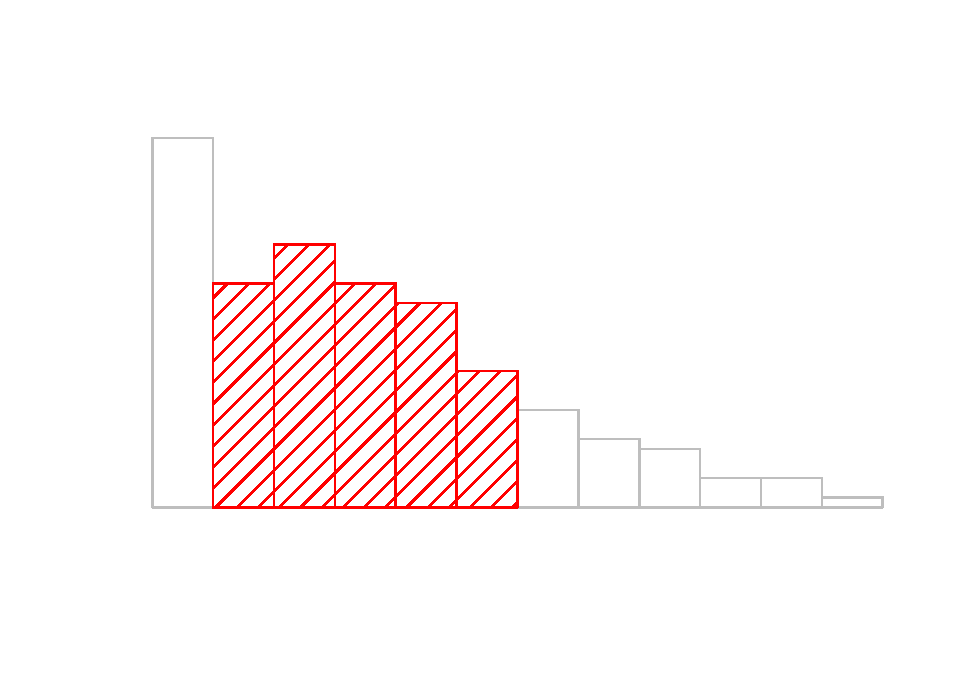
\includegraphics{navarro2_files/figure-latex/aflsd-1.pdf}
\caption{\label{fig:aflsd}An illustration of the standard deviation, applied
to the AFL winning margins data. The shaded bars in the histogram show
how much of the data fall within one standard deviation of the mean. In
this case, 65.3\% of the data set lies within this range, which is
pretty consistent with the ``approximately 68\% rule'' discussed in the
main text.}
\end{figure}

\subsection{Median absolute deviation}\label{mad}

The last measure of variability that I want to talk about is the
\textbf{\emph{median absolute deviation}} (MAD). The basic idea behind
MAD is very simple, and is pretty much identical to the idea behind the
mean absolute deviation (Section \ref{aad}). The difference is that you
use the median everywhere. If we were to frame this idea as a pair of R
commands, they would look like this:

\begin{Shaded}
\begin{Highlighting}[]
\CommentTok{# mean absolute deviation from the mean:}
\KeywordTok{mean}\NormalTok{( }\KeywordTok{abs}\NormalTok{(afl.margins }\OperatorTok{-}\StringTok{ }\KeywordTok{mean}\NormalTok{(afl.margins)) )}
\end{Highlighting}
\end{Shaded}

\begin{verbatim}
## [1] 21.10124
\end{verbatim}

\begin{Shaded}
\begin{Highlighting}[]
\CommentTok{# *median* absolute deviation from the *median*:}
\KeywordTok{median}\NormalTok{( }\KeywordTok{abs}\NormalTok{(afl.margins }\OperatorTok{-}\StringTok{ }\KeywordTok{median}\NormalTok{(afl.margins)) )}
\end{Highlighting}
\end{Shaded}

\begin{verbatim}
## [1] 19.5
\end{verbatim}

This has a straightforward interpretation: every observation in the data
set lies some distance away from the typical value (the median). So the
MAD is an attempt to describe a \emph{typical deviation from a typical
value} in the data set. It wouldn't be unreasonable to interpret the MAD
value of 19.5 for our AFL data by saying something like this:

\begin{quote}
The median winning margin in 2010 was 30.5, indicating that a typical
game involved a winning margin of about 30 points. However, there was a
fair amount of variation from game to game: the MAD value was 19.5,
indicating that a typical winning margin would differ from this median
value by about 19-20 points.
\end{quote}

As you'd expect, R has a built in function for calculating MAD, and you
will be shocked no doubt to hear that it's called \texttt{mad()}.
However, it's a little bit more complicated than the functions that
we've been using previously. If you want to use it to calculate MAD in
the exact same way that I have described it above, the command that you
need to use specifies two arguments: the data set itself \texttt{x}, and
a \texttt{constant} that I'll explain in a moment. For our purposes, the
constant is 1, so our command becomes

\begin{Shaded}
\begin{Highlighting}[]
\KeywordTok{mad}\NormalTok{( }\DataTypeTok{x =}\NormalTok{ afl.margins, }\DataTypeTok{constant =} \DecValTok{1}\NormalTok{ )}
\end{Highlighting}
\end{Shaded}

\begin{verbatim}
## [1] 19.5
\end{verbatim}

Apart from the weirdness of having to type that \texttt{constant\ =\ 1}
part, this is pretty straightforward.

Okay, so what exactly is this \texttt{constant\ =\ 1} argument? I won't
go into all the details here, but here's the gist. Although the ``raw''
MAD value that I've described above is completely interpretable on its
own terms, that's not actually how it's used in a lot of real world
contexts. Instead, what happens a lot is that the researcher
\emph{actually} wants to calculate the standard deviation. However, in
the same way that the mean is very sensitive to extreme values, the
standard deviation is vulnerable to the exact same issue. So, in much
the same way that people sometimes use the median as a ``robust'' way of
calculating ``something that is like the mean'', it's not uncommon to
use MAD as a method for calculating ``something that is like the
standard deviation''. Unfortunately, the \emph{raw} MAD value doesn't do
this. Our raw MAD value is 19.5, and our standard deviation was 26.07.
However, what some clever person has shown is that, under certain
assumptions\footnote{The assumption again being that the data are
  normally-distributed!}, you can multiply the raw MAD value by 1.4826
and obtain a number that is directly comparable to the standard
deviation. As a consequence, the default value of \texttt{constant} is
1.4826, and so when you use the \texttt{mad()} command without manually
setting a value, here's what you get:

\begin{Shaded}
\begin{Highlighting}[]
\KeywordTok{mad}\NormalTok{( afl.margins )}
\end{Highlighting}
\end{Shaded}

\begin{verbatim}
## [1] 28.9107
\end{verbatim}

I should point out, though, that if you want to use this ``corrected''
MAD value as a robust version of the standard deviation, you really are
relying on the assumption that the data are (or at least, are ``supposed
to be'' in some sense) symmetric and basically shaped like a bell curve.
That's really \emph{not} true for our \texttt{afl.margins} data, so in
this case I wouldn't try to use the MAD value this way.

\subsection{Which measure to use?}\label{which-measure-to-use}

We've discussed quite a few measures of spread (range, IQR, MAD,
variance and standard deviation), and hinted at their strengths and
weaknesses. Here's a quick summary:

\begin{itemize}
\tightlist
\item
  \emph{Range}. Gives you the full spread of the data. It's very
  vulnerable to outliers, and as a consequence it isn't often used
  unless you have good reasons to care about the extremes in the data.
\item
  \emph{Interquartile range}. Tells you where the ``middle half'' of the
  data sits. It's pretty robust, and complements the median nicely. This
  is used a lot.
\item
  \emph{Mean absolute deviation}. Tells you how far ``on average'' the
  observations are from the mean. It's very interpretable, but has a few
  minor issues (not discussed here) that make it less attractive to
  statisticians than the standard deviation. Used sometimes, but not
  often.
\item
  \emph{Variance}. Tells you the average squared deviation from the
  mean. It's mathematically elegant, and is probably the ``right'' way
  to describe variation around the mean, but it's completely
  uninterpretable because it doesn't use the same units as the data.
  Almost never used except as a mathematical tool; but it's buried
  ``under the hood'' of a very large number of statistical tools.
\item
  \emph{Standard deviation}. This is the square root of the variance.
  It's fairly elegant mathematically, and it's expressed in the same
  units as the data so it can be interpreted pretty well. In situations
  where the mean is the measure of central tendency, this is the
  default. This is by far the most popular measure of variation.
\item
  \emph{Median absolute deviation}. The typical (i.e., median) deviation
  from the median value. In the raw form it's simple and interpretable;
  in the corrected form it's a robust way to estimate the standard
  deviation, for some kinds of data sets. Not used very often, but it
  does get reported sometimes.
\end{itemize}

In short, the IQR and the standard deviation are easily the two most
common measures used to report the variability of the data; but there
are situations in which the others are used. I've described all of them
in this book because there's a fair chance you'll run into most of these
somewhere.

\section{Skew and kurtosis}\label{skewandkurtosis}

There are two more descriptive statistics that you will sometimes see
reported in the psychological literature, known as skew and kurtosis. In
practice, neither one is used anywhere near as frequently as the
measures of central tendency and variability that we've been talking
about. Skew is pretty important, so you do see it mentioned a fair bit;
but I've actually never seen kurtosis reported in a scientific article
to date.

\begin{verbatim}
## [1] -0.9226009
\end{verbatim}

\begin{verbatim}
## [1] -0.000196261
\end{verbatim}

\begin{figure}
\centering
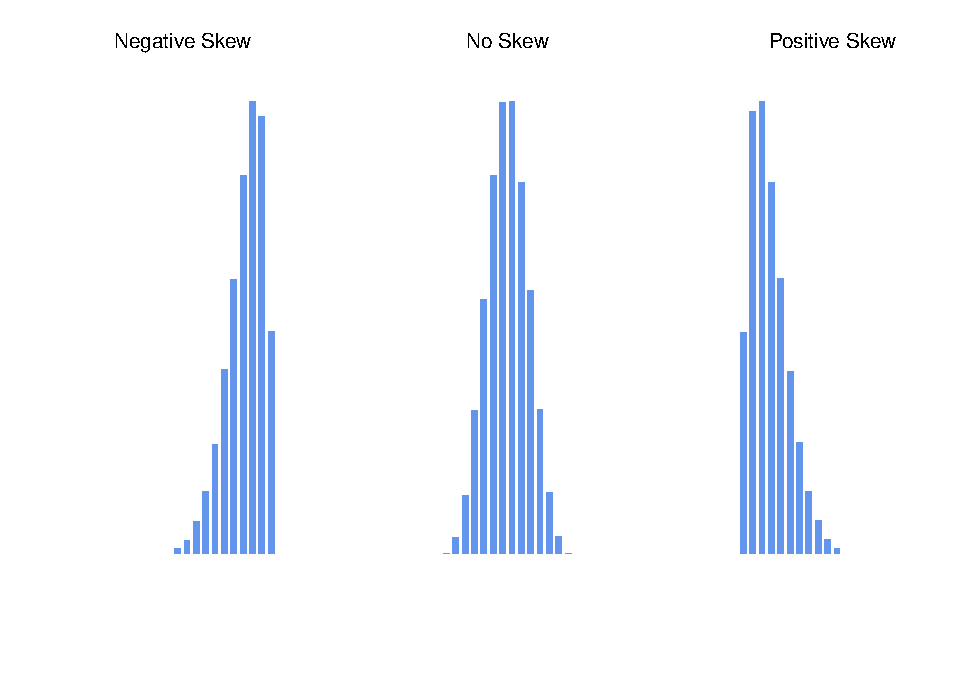
\includegraphics{navarro2_files/figure-latex/skewness-1.pdf}
\caption{\label{fig:skewness}An illustration of skewness. On the left we
have a negatively skewed data set (skewness \(= -.93\)), in the middle
we have a data set with no skew (technically, skewness \(= -.006\)), and
on the right we have a positively skewed data set (skewness \(= .93\)).}
\end{figure}

\begin{verbatim}
## [1] 0.9183211
\end{verbatim}

Since it's the more interesting of the two, let's start by talking about
the \textbf{\emph{skewness}}. Skewness is basically a measure of
asymmetry, and the easiest way to explain it is by drawing some
pictures. As Figure \ref{fig:skewness} illustrates, if the data tend to
have a lot of extreme small values (i.e., the lower tail is ``longer''
than the upper tail) and not so many extremely large values (left
panel), then we say that the data are \emph{negatively skewed}. On the
other hand, if there are more extremely large values than extremely
small ones (right panel) we say that the data are \emph{positively
skewed}. That's the qualitative idea behind skewness. The actual formula
for the skewness of a data set is as follows \[
\mbox{skewness}(X) = \frac{1}{N \hat{\sigma}^3} \sum_{i=1}^N (X_i - \bar{X})^3
\] where \(N\) is the number of observations, \(\bar{X}\) is the sample
mean, and \(\hat{\sigma}\) is the standard deviation (the ``divide by
\(N-1\)'' version, that is). Perhaps more helpfully, it might be useful
to point out that the \texttt{psych} package contains a \texttt{skew()}
function that you can use to calculate skewness. So if we wanted to use
this function to calculate the skewness of the \texttt{afl.margins}
data, we'd first need to load the package

\begin{Shaded}
\begin{Highlighting}[]
\KeywordTok{library}\NormalTok{( psych )}
\end{Highlighting}
\end{Shaded}

which now makes it possible to use the following command:

\begin{Shaded}
\begin{Highlighting}[]
\KeywordTok{skew}\NormalTok{( }\DataTypeTok{x =}\NormalTok{ afl.margins )}
\end{Highlighting}
\end{Shaded}

\begin{verbatim}
## [1] 0.7671555
\end{verbatim}

Not surprisingly, it turns out that the AFL winning margins data is
fairly skewed.

The final measure that is sometimes referred to, though very rarely in
practice, is the \textbf{\emph{kurtosis}} of a data set. Put simply,
kurtosis is a measure of the ``pointiness'' of a data set, as
illustrated in Figure \ref{fig:kurtosis}.

\begin{verbatim}
## [1] -0.9562248
\end{verbatim}

\begin{verbatim}
## [1] 0.001793924
\end{verbatim}

\begin{figure}
\centering
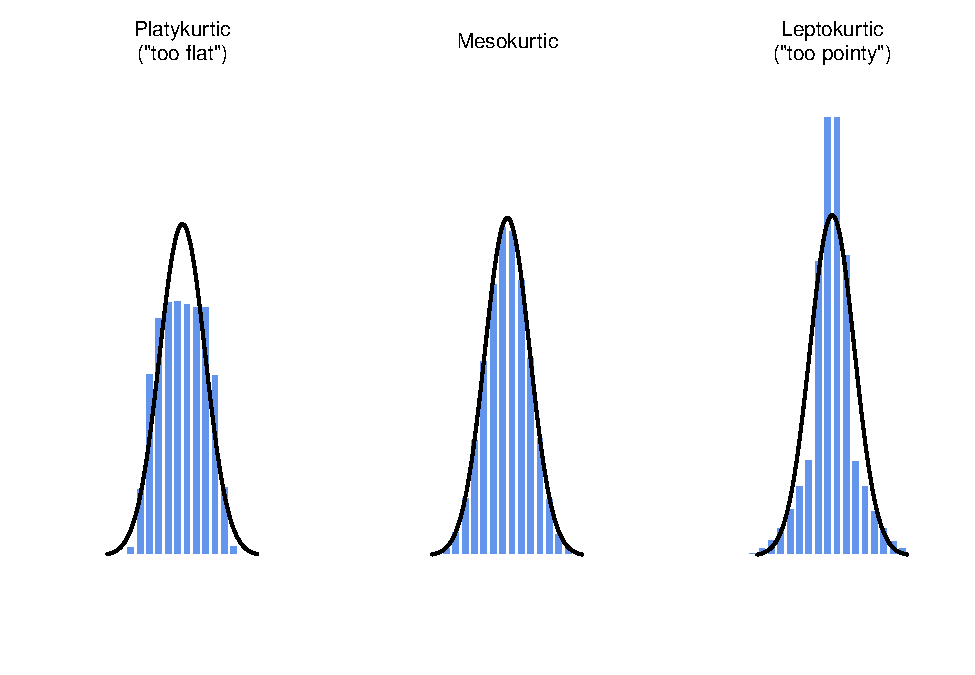
\includegraphics{navarro2_files/figure-latex/kurtosis-1.pdf}
\caption{\label{fig:kurtosis}An illustration of kurtosis. On the left, we
have a ``platykurtic'' data set (kurtosis = \(-.95\)), meaning that the
data set is ``too flat''. In the middle we have a ``mesokurtic'' data
set (kurtosis is almost exactly 0), which means that the pointiness of
the data is just about right. Finally, on the right, we have a
``leptokurtic'' data set (kurtosis \(= 2.12\)) indicating that the data
set is ``too pointy''. Note that kurtosis is measured with respect to a
normal curve (black line)}
\end{figure}

\begin{verbatim}
## [1] 2.056246
\end{verbatim}

By convention, we say that the ``normal curve'' (black lines) has zero
kurtosis, so the pointiness of a data set is assessed relative to this
curve. In this Figure, the data on the left are not pointy enough, so
the kurtosis is negative and we call the data \emph{platykurtic}. The
data on the right are too pointy, so the kurtosis is positive and we say
that the data is \emph{leptokurtic}. But the data in the middle are just
pointy enough, so we say that it is \emph{mesokurtic} and has kurtosis
zero. This is summarised in the table below:

\begin{tabular}{lll}
\toprule
informal term & technical name & kurtosis value\\
\midrule
too flat & platykurtic & negative\\
just pointy enough & mesokurtic & zero\\
too pointy & leptokurtic & positive\\
\bottomrule
\end{tabular}

The equation for kurtosis is pretty similar in spirit to the formulas
we've seen already for the variance and the skewness; except that where
the variance involved squared deviations and the skewness involved cubed
deviations, the kurtosis involves raising the deviations to the fourth
power:\footnote{The ``\(-3\)'' part is something that statisticians tack
  on to ensure that the normal curve has kurtosis zero. It looks a bit
  stupid, just sticking a ``-3'' at the end of the formula, but there
  are good mathematical reasons for doing this.} \[
\mbox{kurtosis}(X) = \frac{1}{N \hat\sigma^4} \sum_{i=1}^N \left( X_i - \bar{X} \right)^4  - 3
\] I know, it's not terribly interesting to me either. More to the
point, the \texttt{psych} package has a function called
\texttt{kurtosi()} that you can use to calculate the kurtosis of your
data. For instance, if we were to do this for the AFL margins,

\begin{Shaded}
\begin{Highlighting}[]
\KeywordTok{kurtosi}\NormalTok{( }\DataTypeTok{x =}\NormalTok{ afl.margins )}
\end{Highlighting}
\end{Shaded}

\begin{verbatim}
## [1] 0.02962633
\end{verbatim}

we discover that the AFL winning margins data are just pointy enough.

\section{Getting an overall summary of a variable}\label{summary}

Up to this point in the chapter I've explained several different summary
statistics that are commonly used when analysing data, along with
specific functions that you can use in R to calculate each one. However,
it's kind of annoying to have to separately calculate means, medians,
standard deviations, skews etc. Wouldn't it be nice if R had some
helpful functions that would do all these tedious calculations at once?
Something like \texttt{summary()} or \texttt{describe()}, perhaps? Why
yes, yes it would. So much so that both of these functions exist. The
\texttt{summary()} function is in the \texttt{base} package, so it comes
with every installation of R. The \texttt{describe()} function is part
of the \texttt{psych} package, which we loaded earlier in the chapter.

\subsection{\texorpdfstring{``Summarising'' a
variable}{Summarising a variable}}\label{summarising-a-variable}

The \texttt{summary()} function is an easy thing to use, but a tricky
thing to understand in full, since it's a generic function (see Section
\ref{generics}. The basic idea behind the \texttt{summary()} function is
that it prints out some useful information about whatever object (i.e.,
variable, as far as we're concerned) you specify as the \texttt{object}
argument. As a consequence, the behaviour of the \texttt{summary()}
function differs quite dramatically depending on the class of the object
that you give it. Let's start by giving it a \emph{numeric} object:

\begin{Shaded}
\begin{Highlighting}[]
\KeywordTok{summary}\NormalTok{( }\DataTypeTok{object =}\NormalTok{ afl.margins )  }
\end{Highlighting}
\end{Shaded}

\begin{verbatim}
##    Min. 1st Qu.  Median    Mean 3rd Qu.    Max. 
##    0.00   12.75   30.50   35.30   50.50  116.00
\end{verbatim}

For numeric variables, we get a whole bunch of useful descriptive
statistics. It gives us the minimum and maximum values (i.e., the
range), the first and third quartiles (25th and 75th percentiles; i.e.,
the IQR), the mean and the median. In other words, it gives us a pretty
good collection of descriptive statistics related to the central
tendency and the spread of the data.

Okay, what about if we feed it a logical vector instead? Let's say I
want to know something about how many ``blowouts'' there were in the
2010 AFL season. I operationalise the concept of a blowout (see Chapter
\ref{studydesign}) as a game in which the winning margin exceeds 50
points. Let's create a logical variable \texttt{blowouts} in which the
\(i\)-th element is \texttt{TRUE} if that game was a blowout according
to my definition,

\begin{Shaded}
\begin{Highlighting}[]
\NormalTok{blowouts <-}\StringTok{  }\NormalTok{afl.margins }\OperatorTok{>}\StringTok{ }\DecValTok{50}
\NormalTok{blowouts}
\end{Highlighting}
\end{Shaded}

\begin{verbatim}
##   [1]  TRUE FALSE  TRUE FALSE FALSE FALSE FALSE  TRUE FALSE FALSE FALSE
##  [12]  TRUE FALSE FALSE  TRUE FALSE FALSE FALSE FALSE  TRUE FALSE FALSE
##  [23] FALSE FALSE FALSE FALSE FALSE  TRUE FALSE  TRUE  TRUE FALSE FALSE
##  [34]  TRUE FALSE FALSE  TRUE FALSE FALSE FALSE FALSE FALSE FALSE FALSE
##  [45] FALSE  TRUE  TRUE FALSE FALSE FALSE FALSE FALSE  TRUE  TRUE FALSE
##  [56]  TRUE FALSE FALSE FALSE FALSE  TRUE FALSE FALSE FALSE FALSE FALSE
##  [67]  TRUE FALSE FALSE FALSE FALSE FALSE FALSE  TRUE FALSE FALSE FALSE
##  [78] FALSE FALSE  TRUE FALSE FALSE FALSE FALSE FALSE FALSE FALSE FALSE
##  [89] FALSE FALSE  TRUE FALSE FALSE  TRUE FALSE FALSE FALSE FALSE FALSE
## [100] FALSE  TRUE FALSE FALSE FALSE  TRUE FALSE  TRUE  TRUE  TRUE FALSE
## [111] FALSE FALSE FALSE FALSE FALSE FALSE FALSE FALSE FALSE  TRUE FALSE
## [122]  TRUE FALSE FALSE FALSE FALSE FALSE FALSE FALSE  TRUE  TRUE FALSE
## [133] FALSE  TRUE  TRUE FALSE FALSE FALSE FALSE FALSE  TRUE FALSE  TRUE
## [144]  TRUE  TRUE  TRUE FALSE FALSE FALSE  TRUE FALSE FALSE  TRUE FALSE
## [155]  TRUE FALSE  TRUE FALSE FALSE  TRUE FALSE FALSE  TRUE FALSE FALSE
## [166] FALSE FALSE FALSE FALSE FALSE FALSE FALSE FALSE FALSE FALSE FALSE
\end{verbatim}

So that's what the \texttt{blowouts} variable looks like. Now let's ask
R for a \texttt{summary()}

\begin{Shaded}
\begin{Highlighting}[]
\KeywordTok{summary}\NormalTok{( }\DataTypeTok{object =}\NormalTok{ blowouts )}
\end{Highlighting}
\end{Shaded}

\begin{verbatim}
##    Mode   FALSE    TRUE 
## logical     132      44
\end{verbatim}

In this context, the \texttt{summary()} function gives us a count of the
number of \texttt{TRUE} values, the number of \texttt{FALSE} values, and
the number of missing values (i.e., the \texttt{NA}s). Pretty reasonable
behaviour.

Next, let's try to give it a factor. If you recall, I've defined the
\texttt{afl.finalists} vector as a factor, so let's use that:

\begin{Shaded}
\begin{Highlighting}[]
\KeywordTok{summary}\NormalTok{( }\DataTypeTok{object =}\NormalTok{ afl.finalists )}
\end{Highlighting}
\end{Shaded}

\begin{verbatim}
##         Adelaide         Brisbane          Carlton      Collingwood 
##               26               25               26               28 
##         Essendon          Fitzroy        Fremantle          Geelong 
##               32                0                6               39 
##         Hawthorn        Melbourne  North Melbourne    Port Adelaide 
##               27               28               28               17 
##         Richmond         St Kilda           Sydney       West Coast 
##                6               24               26               38 
## Western Bulldogs 
##               24
\end{verbatim}

For factors, we get a frequency table, just like we got when we used the
\texttt{table()} function. Interestingly, however, if we convert this to
a character vector using the \texttt{as.character()} function (see
Section \ref{coercion}, we don't get the same results:

\begin{Shaded}
\begin{Highlighting}[]
\NormalTok{f2 <-}\StringTok{ }\KeywordTok{as.character}\NormalTok{( afl.finalists )}
\KeywordTok{summary}\NormalTok{( }\DataTypeTok{object =}\NormalTok{ f2 )}
\end{Highlighting}
\end{Shaded}

\begin{verbatim}
##    Length     Class      Mode 
##       400 character character
\end{verbatim}

This is one of those situations I was referring to in Section
\ref{factors}, in which it is helpful to declare your nominal scale
variable as a factor rather than a character vector. Because I've
defined \texttt{afl.finalists} as a factor, R \emph{knows} that it
should treat it as a nominal scale variable, and so it gives you a much
more detailed (and helpful) summary than it would have if I'd left it as
a character vector.

\subsection{\texorpdfstring{``Summarising'' a data
frame}{Summarising a data frame}}\label{summarising-a-data-frame}

Okay what about data frames? When you pass a data frame to the
\texttt{summary()} function, it produces a slightly condensed summary of
each variable inside the data frame. To give you a sense of how this can
be useful, let's try this for a new data set, one that you've never seen
before. The data is stored in the \texttt{clinicaltrial.Rdata} file, and
we'll use it a lot in Chapter \ref{anova} (you can find a complete
description of the data at the start of that chapter). Let's load it,
and see what we've got:

\begin{Shaded}
\begin{Highlighting}[]
\KeywordTok{load}\NormalTok{( }\StringTok{"./data/clinicaltrial.Rdata"}\NormalTok{ )}
\KeywordTok{who}\NormalTok{(}\OtherTok{TRUE}\NormalTok{)}
\end{Highlighting}
\end{Shaded}

\begin{verbatim}
##    -- Name --    -- Class --   -- Size --
##    clin.trial    data.frame    18 x 3    
##     $drug        factor        18        
##     $therapy     factor        18        
##     $mood.gain   numeric       18
\end{verbatim}

There's a single data frame called \texttt{clin.trial} which contains
three variables, \texttt{drug}, \texttt{therapy} and \texttt{mood.gain}.
Presumably then, this data is from a clinical trial of some kind, in
which people were administered different drugs; and the researchers
looked to see what the drugs did to their mood. Let's see if the
\texttt{summary()} function sheds a little more light on this situation:

\begin{Shaded}
\begin{Highlighting}[]
\KeywordTok{summary}\NormalTok{( clin.trial )}
\end{Highlighting}
\end{Shaded}

\begin{verbatim}
##        drug         therapy    mood.gain     
##  placebo :6   no.therapy:9   Min.   :0.1000  
##  anxifree:6   CBT       :9   1st Qu.:0.4250  
##  joyzepam:6                  Median :0.8500  
##                              Mean   :0.8833  
##                              3rd Qu.:1.3000  
##                              Max.   :1.8000
\end{verbatim}

Evidently there were three drugs: a placebo, something called
``anxifree'' and something called ``joyzepam''; and there were 6 people
administered each drug. There were 9 people treated using cognitive
behavioural therapy (CBT) and 9 people who received no psychological
treatment. And we can see from looking at the summary of the
\texttt{mood.gain} variable that most people did show a mood gain (mean
\(=.88\)), though without knowing what the scale is here it's hard to
say much more than that. Still, that's not too bad. Overall, I feel that
I learned something from that.

\subsection{\texorpdfstring{``Describing'' a data
frame}{Describing a data frame}}\label{describing-a-data-frame}

The \texttt{describe()} function (in the \texttt{psych} package) is a
little different, and it's really only intended to be useful when your
data are interval or ratio scale. Unlike the \texttt{summary()}
function, it calculates the same descriptive statistics for any type of
variable you give it. By default, these are:

\begin{itemize}
\tightlist
\item
  \texttt{var}. This is just an index: 1 for the first variable, 2 for
  the second variable, and so on.
\item
  \texttt{n}. This is the sample size: more precisely, it's the number
  of non-missing values.
\item
  \texttt{mean}. This is the sample mean (Section \ref{mean}).
\item
  \texttt{sd}. This is the (bias corrected) standard deviation (Section
  \ref{sd}).
\item
  \texttt{median}. The median (Section \ref{median}).
\item
  \texttt{trimmed}. This is trimmed mean. By default it's the 10\%
  trimmed mean (Section \ref{trimmedmean}).
\item
  \texttt{mad}. The median absolute deviation (Section \ref{mad}).
\item
  \texttt{min}. The minimum value.
\item
  \texttt{max}. The maximum value.
\item
  \texttt{range}. The range spanned by the data (Section \ref{range}).
\item
  \texttt{skew}. The skewness (Section \ref{skewandkurtosis}).
\item
  \texttt{kurtosis}. The kurtosis (Section \ref{skewandkurtosis}).
\item
  \texttt{se}. The standard error of the mean (Chapter
  \ref{estimation}).
\end{itemize}

Notice that these descriptive statistics generally only make sense for
data that are interval or ratio scale (usually encoded as numeric
vectors). For nominal or ordinal variables (usually encoded as factors),
most of these descriptive statistics are not all that useful. What the
\texttt{describe()} function does is convert factors and logical
variables to numeric vectors in order to do the calculations. These
variables are marked with \texttt{*} and most of the time, the
descriptive statistics for those variables won't make much sense. If you
try to feed it a data frame that includes a character vector as a
variable, it produces an error.

With those caveats in mind, let's use the \texttt{describe()} function
to have a look at the \texttt{clin.trial} data frame. Here's what we
get:

\begin{Shaded}
\begin{Highlighting}[]
\KeywordTok{describe}\NormalTok{( }\DataTypeTok{x =}\NormalTok{ clin.trial )}
\end{Highlighting}
\end{Shaded}

\begin{verbatim}
##           vars  n mean   sd median trimmed  mad min max range skew
## drug*        1 18 2.00 0.84   2.00    2.00 1.48 1.0 3.0   2.0 0.00
## therapy*     2 18 1.50 0.51   1.50    1.50 0.74 1.0 2.0   1.0 0.00
## mood.gain    3 18 0.88 0.53   0.85    0.88 0.67 0.1 1.8   1.7 0.13
##           kurtosis   se
## drug*        -1.66 0.20
## therapy*     -2.11 0.12
## mood.gain    -1.44 0.13
\end{verbatim}

As you can see, the output for the asterisked variables is pretty
meaningless, and should be ignored. However, for the \texttt{mood.gain}
variable, there's a lot of useful information.

\section{Descriptive statistics separately for each
group}\label{groupdescriptives}

It is very commonly the case that you find yourself needing to look at
descriptive statistics, broken down by some grouping variable. This is
pretty easy to do in R, and there are three functions in particular that
are worth knowing about: \texttt{by()}, \texttt{describeBy()} and
\texttt{aggregate()}. Let's start with the \texttt{describeBy()}
function, which is part of the \texttt{psych} package. The
\texttt{describeBy()} function is very similar to the
\texttt{describe()} function, except that it has an additional argument
called \texttt{group} which specifies a grouping variable. For instance,
let's say, I want to look at the descriptive statistics for the
\texttt{clin.trial} data, broken down separately by \texttt{therapy}
type. The command I would use here is:

\begin{Shaded}
\begin{Highlighting}[]
\KeywordTok{describeBy}\NormalTok{( }\DataTypeTok{x=}\NormalTok{clin.trial, }\DataTypeTok{group=}\NormalTok{clin.trial}\OperatorTok{$}\NormalTok{therapy )}
\end{Highlighting}
\end{Shaded}

\begin{verbatim}
## 
##  Descriptive statistics by group 
## group: no.therapy
##           vars n mean   sd median trimmed  mad min max range skew kurtosis
## drug*        1 9 2.00 0.87    2.0    2.00 1.48 1.0 3.0   2.0 0.00    -1.81
## therapy*     2 9 1.00 0.00    1.0    1.00 0.00 1.0 1.0   0.0  NaN      NaN
## mood.gain    3 9 0.72 0.59    0.5    0.72 0.44 0.1 1.7   1.6 0.51    -1.59
##             se
## drug*     0.29
## therapy*  0.00
## mood.gain 0.20
## -------------------------------------------------------- 
## group: CBT
##           vars n mean   sd median trimmed  mad min max range  skew
## drug*        1 9 2.00 0.87    2.0    2.00 1.48 1.0 3.0   2.0  0.00
## therapy*     2 9 2.00 0.00    2.0    2.00 0.00 2.0 2.0   0.0   NaN
## mood.gain    3 9 1.04 0.45    1.1    1.04 0.44 0.3 1.8   1.5 -0.03
##           kurtosis   se
## drug*        -1.81 0.29
## therapy*       NaN 0.00
## mood.gain    -1.12 0.15
\end{verbatim}

As you can see, the output is essentially identical to the output that
the \texttt{describe()} function produce, except that the output now
gives you means, standard deviations etc separately for the \texttt{CBT}
group and the \texttt{no.therapy} group. Notice that, as before, the
output displays asterisks for factor variables, in order to draw your
attention to the fact that the descriptive statistics that it has
calculated won't be very meaningful for those variables. Nevertheless,
this command has given us some really useful descriptive statistics
\texttt{mood.gain} variable, broken down as a function of
\texttt{therapy}.

A somewhat more general solution is offered by the \texttt{by()}
function. There are three arguments that you need to specify when using
this function: the \texttt{data} argument specifies the data set, the
\texttt{INDICES} argument specifies the grouping variable, and the
\texttt{FUN} argument specifies the name of a function that you want to
apply separately to each group. To give a sense of how powerful this is,
you can reproduce the \texttt{describeBy()} function by using a command
like this:

\begin{Shaded}
\begin{Highlighting}[]
\KeywordTok{by}\NormalTok{( }\DataTypeTok{data=}\NormalTok{clin.trial, }\DataTypeTok{INDICES=}\NormalTok{clin.trial}\OperatorTok{$}\NormalTok{therapy, }\DataTypeTok{FUN=}\NormalTok{describe )}
\end{Highlighting}
\end{Shaded}

\begin{verbatim}
## clin.trial$therapy: no.therapy
##           vars n mean   sd median trimmed  mad min max range skew kurtosis
## drug*        1 9 2.00 0.87    2.0    2.00 1.48 1.0 3.0   2.0 0.00    -1.81
## therapy*     2 9 1.00 0.00    1.0    1.00 0.00 1.0 1.0   0.0  NaN      NaN
## mood.gain    3 9 0.72 0.59    0.5    0.72 0.44 0.1 1.7   1.6 0.51    -1.59
##             se
## drug*     0.29
## therapy*  0.00
## mood.gain 0.20
## -------------------------------------------------------- 
## clin.trial$therapy: CBT
##           vars n mean   sd median trimmed  mad min max range  skew
## drug*        1 9 2.00 0.87    2.0    2.00 1.48 1.0 3.0   2.0  0.00
## therapy*     2 9 2.00 0.00    2.0    2.00 0.00 2.0 2.0   0.0   NaN
## mood.gain    3 9 1.04 0.45    1.1    1.04 0.44 0.3 1.8   1.5 -0.03
##           kurtosis   se
## drug*        -1.81 0.29
## therapy*       NaN 0.00
## mood.gain    -1.12 0.15
\end{verbatim}

This will produce the exact same output as the command shown earlier.
However, there's nothing special about the \texttt{describe()} function.
You could just as easily use the \texttt{by()} function in conjunction
with the \texttt{summary()} function. For example:

\begin{Shaded}
\begin{Highlighting}[]
\KeywordTok{by}\NormalTok{( }\DataTypeTok{data=}\NormalTok{clin.trial, }\DataTypeTok{INDICES=}\NormalTok{clin.trial}\OperatorTok{$}\NormalTok{therapy, }\DataTypeTok{FUN=}\NormalTok{summary )}
\end{Highlighting}
\end{Shaded}

\begin{verbatim}
## clin.trial$therapy: no.therapy
##        drug         therapy    mood.gain     
##  placebo :3   no.therapy:9   Min.   :0.1000  
##  anxifree:3   CBT       :0   1st Qu.:0.3000  
##  joyzepam:3                  Median :0.5000  
##                              Mean   :0.7222  
##                              3rd Qu.:1.3000  
##                              Max.   :1.7000  
## -------------------------------------------------------- 
## clin.trial$therapy: CBT
##        drug         therapy    mood.gain    
##  placebo :3   no.therapy:0   Min.   :0.300  
##  anxifree:3   CBT       :9   1st Qu.:0.800  
##  joyzepam:3                  Median :1.100  
##                              Mean   :1.044  
##                              3rd Qu.:1.300  
##                              Max.   :1.800
\end{verbatim}

Again, this output is pretty easy to interpret. It's the output of the
\texttt{summary()} function, applied separately to \texttt{CBT} group
and the \texttt{no.therapy} group. For the two factors (\texttt{drug}
and \texttt{therapy}) it prints out a frequency table, whereas for the
numeric variable (\texttt{mood.gain}) it prints out the range,
interquartile range, mean and median.

What if you have multiple grouping variables? Suppose, for example, you
would like to look at the average mood gain separately for all possible
combinations of drug and therapy. It is actually possible to do this
using the \texttt{by()} and \texttt{describeBy()} functions, but I
usually find it more convenient to use the \texttt{aggregate()} function
in this situation. There are again three arguments that you need to
specify. The \texttt{formula} argument is used to indicate which
variable you want to analyse, and which variables are used to specify
the groups. For instance, if you want to look at \texttt{mood.gain}
separately for each possible combination of \texttt{drug} and
\texttt{therapy}, the formula you want is
\texttt{mood.gain\ \textasciitilde{}\ drug\ +\ therapy}. The
\texttt{data} argument is used to specify the data frame containing all
the data, and the \texttt{FUN} argument is used to indicate what
function you want to calculate for each group (e.g., the \texttt{mean}).
So, to obtain group means, use this command:

\begin{Shaded}
\begin{Highlighting}[]
 \KeywordTok{aggregate}\NormalTok{( }\DataTypeTok{formula =}\NormalTok{ mood.gain }\OperatorTok{~}\StringTok{ }\NormalTok{drug }\OperatorTok{+}\StringTok{ }\NormalTok{therapy,  }\CommentTok{# mood.gain by drug/therapy combination}
            \DataTypeTok{data =}\NormalTok{ clin.trial,                     }\CommentTok{# data is in the clin.trial data frame}
            \DataTypeTok{FUN =}\NormalTok{ mean                             }\CommentTok{# print out group means}
\NormalTok{ )}
\end{Highlighting}
\end{Shaded}

\begin{verbatim}
##       drug    therapy mood.gain
## 1  placebo no.therapy  0.300000
## 2 anxifree no.therapy  0.400000
## 3 joyzepam no.therapy  1.466667
## 4  placebo        CBT  0.600000
## 5 anxifree        CBT  1.033333
## 6 joyzepam        CBT  1.500000
\end{verbatim}

or, alternatively, if you want to calculate the standard deviations for
each group, you would use the following command (argument names omitted
this time):

\begin{Shaded}
\begin{Highlighting}[]
\KeywordTok{aggregate}\NormalTok{( mood.gain }\OperatorTok{~}\StringTok{ }\NormalTok{drug }\OperatorTok{+}\StringTok{ }\NormalTok{therapy, clin.trial, sd )}
\end{Highlighting}
\end{Shaded}

\begin{verbatim}
##       drug    therapy mood.gain
## 1  placebo no.therapy 0.2000000
## 2 anxifree no.therapy 0.2000000
## 3 joyzepam no.therapy 0.2081666
## 4  placebo        CBT 0.3000000
## 5 anxifree        CBT 0.2081666
## 6 joyzepam        CBT 0.2645751
\end{verbatim}

\section{Standard scores}\label{zscore}

Suppose my friend is putting together a new questionnaire intended to
measure ``grumpiness''. The survey has 50 questions, which you can
answer in a grumpy way or not. Across a big sample (hypothetically,
let's imagine a million people or so!) the data are fairly normally
distributed, with the mean grumpiness score being 17 out of 50 questions
answered in a grumpy way, and the standard deviation is 5. In contrast,
when I take the questionnaire, I answer 35 out of 50 questions in a
grumpy way. So, how grumpy am I? One way to think about would be to say
that I have grumpiness of 35/50, so you might say that I'm 70\% grumpy.
But that's a bit weird, when you think about it. If my friend had
phrased her questions a bit differently, people might have answered them
in a different way, so the overall distribution of answers could easily
move up or down depending on the precise way in which the questions were
asked. So, I'm only 70\% grumpy \emph{with respect to this set of survey
questions}. Even if it's a very good questionnaire, this isn't very a
informative statement.

A simpler way around this is to describe my grumpiness by comparing me
to other people. Shockingly, out of my friend's sample of 1,000,000
people, only 159 people were as grumpy as me (that's not at all
unrealistic, frankly), suggesting that I'm in the top 0.016\% of people
for grumpiness. This makes much more sense than trying to interpret the
raw data. This idea -- that we should describe my grumpiness in terms of
the overall distribution of the grumpiness of humans -- is the
qualitative idea that standardisation attempts to get at. One way to do
this is to do exactly what I just did, and describe everything in terms
of percentiles. However, the problem with doing this is that ``it's
lonely at the top''. Suppose that my friend had only collected a sample
of 1000 people (still a pretty big sample for the purposes of testing a
new questionnaire, I'd like to add), and this time gotten a mean of 16
out of 50 with a standard deviation of 5, let's say. The problem is that
almost certainly, not a single person in that sample would be as grumpy
as me.

However, all is not lost. A different approach is to convert my
grumpiness score into a \textbf{\emph{standard score}}, also referred to
as a \(z\)-score. The standard score is defined as the number of
standard deviations above the mean that my grumpiness score lies. To
phrase it in ``pseudo-maths'' the standard score is calculated like
this: \[
\mbox{standard score} = \frac{\mbox{raw score} - \mbox{mean}}{\mbox{standard deviation}}
\] In actual maths, the equation for the \(z\)-score is \[
z_i = \frac{X_i - \bar{X}}{\hat\sigma}
\] So, going back to the grumpiness data, we can now transform Dan's raw
grumpiness into a standardised grumpiness score.\footnote{I haven't
  discussed how to compute \(z\)-scores, explicitly, but you can
  probably guess. For a variable \texttt{X}, the simplest way is to use
  a command like \texttt{(X\ -\ mean(X))\ /\ sd(X)}. There's also a
  fancier function called \texttt{scale()} that you can use, but it
  relies on somewhat more complicated R concepts that I haven't
  explained yet.} If the mean is 17 and the standard deviation is 5 then
my standardised grumpiness score would be\footnote{Technically, because
  I'm calculating means and standard deviations from a sample of data,
  but want to talk about my grumpiness relative to a population, what
  I'm actually doing is \emph{estimating} a \(z\) score. However, since
  we haven't talked about estimation yet (see Chapter \ref{estimation})
  I think it's best to ignore this subtlety, especially as it makes very
  little difference to our calculations.} \[
z = \frac{35 - 17}{5} = 3.6
\] To interpret this value, recall the rough heuristic that I provided
in Section \ref{sd}, in which I noted that 99.7\% of values are expected
to lie within 3 standard deviations of the mean. So the fact that my
grumpiness corresponds to a \(z\) score of 3.6 indicates that I'm very
grumpy indeed. Later on, in Section \ref{normal}, I'll introduce a
function called \texttt{pnorm()} that allows us to be a bit more precise
than this. Specifically, it allows us to calculate a theoretical
percentile rank for my grumpiness, as follows:

\begin{Shaded}
\begin{Highlighting}[]
\KeywordTok{pnorm}\NormalTok{( }\FloatTok{3.6}\NormalTok{ )}
\end{Highlighting}
\end{Shaded}

\begin{verbatim}
## [1] 0.9998409
\end{verbatim}

At this stage, this command doesn't make too much sense, but don't worry
too much about it. It's not important for now. But the output is fairly
straightforward: it suggests that I'm grumpier than 99.98\% of people.
Sounds about right.

In addition to allowing you to interpret a raw score in relation to a
larger population (and thereby allowing you to make sense of variables
that lie on arbitrary scales), standard scores serve a second useful
function. Standard scores can be compared to one another in situations
where the raw scores can't. Suppose, for instance, my friend also had
another questionnaire that measured extraversion using a 24 items
questionnaire. The overall mean for this measure turns out to be 13 with
standard deviation 4; and I scored a 2. As you can imagine, it doesn't
make a lot of sense to try to compare my raw score of 2 on the
extraversion questionnaire to my raw score of 35 on the grumpiness
questionnaire. The raw scores for the two variables are ``about''
fundamentally different things, so this would be like comparing apples
to oranges.

What about the standard scores? Well, this is a little different. If we
calculate the standard scores, we get \(z = (35-17)/5 = 3.6\) for
grumpiness and \(z = (2-13)/4 = -2.75\) for extraversion. These two
numbers \emph{can} be compared to each other.\footnote{Though some
  caution is usually warranted. It's not always the case that one
  standard deviation on variable A corresponds to the same ``kind'' of
  thing as one standard deviation on variable B. Use common sense when
  trying to determine whether or not the \(z\) scores of two variables
  can be meaningfully compared.} I'm much less extraverted than most
people (\(z = -2.75\)) and much grumpier than most people (\(z = 3.6\)):
but the extent of my unusualness is much more extreme for grumpiness
(since 3.6 is a bigger number than 2.75). Because each standardised
score is a statement about where an observation falls \emph{relative to
its own population}, it \emph{is} possible to compare standardised
scores across completely different variables.

\section{Correlations}\label{correl}

Up to this point we have focused entirely on how to construct
descriptive statistics for a single variable. What we haven't done is
talked about how to describe the relationships \emph{between} variables
in the data. To do that, we want to talk mostly about the
\textbf{\emph{correlation}} between variables. But first, we need some
data.

\subsection{The data}\label{the-data}

After spending so much time looking at the AFL data, I'm starting to get
bored with sports. Instead, let's turn to a topic close to every
parent's heart: sleep. The following data set is fictitious, but based
on real events. Suppose I'm curious to find out how much my infant son's
sleeping habits affect my mood. Let's say that I can rate my grumpiness
very precisely, on a scale from 0 (not at all grumpy) to 100 (grumpy as
a very, very grumpy old man). And, lets also assume that I've been
measuring my grumpiness, my sleeping patterns and my son's sleeping
patterns for quite some time now. Let's say, for 100 days. And, being a
nerd, I've saved the data as a file called \texttt{parenthood.Rdata}. If
we load the data\ldots{}

\begin{Shaded}
\begin{Highlighting}[]
\KeywordTok{load}\NormalTok{( }\StringTok{"./data/parenthood.Rdata"}\NormalTok{ )}
\KeywordTok{who}\NormalTok{(}\OtherTok{TRUE}\NormalTok{)}
\end{Highlighting}
\end{Shaded}

\begin{verbatim}
##    -- Name --     -- Class --   -- Size --
##    parenthood     data.frame    100 x 4   
##     $dan.sleep    numeric       100       
##     $baby.sleep   numeric       100       
##     $dan.grump    numeric       100       
##     $day          integer       100
\end{verbatim}

\ldots{} we see that the file contains a single data frame called
\texttt{parenthood}, which contains four variables \texttt{dan.sleep},
\texttt{baby.sleep}, \texttt{dan.grump} and \texttt{day}. If we peek at
the data using \texttt{head()} out the data, here's what we get:

\begin{Shaded}
\begin{Highlighting}[]
\KeywordTok{head}\NormalTok{(parenthood,}\DecValTok{10}\NormalTok{)}
\end{Highlighting}
\end{Shaded}

\begin{verbatim}
##    dan.sleep baby.sleep dan.grump day
## 1       7.59      10.18        56   1
## 2       7.91      11.66        60   2
## 3       5.14       7.92        82   3
## 4       7.71       9.61        55   4
## 5       6.68       9.75        67   5
## 6       5.99       5.04        72   6
## 7       8.19      10.45        53   7
## 8       7.19       8.27        60   8
## 9       7.40       6.06        60   9
## 10      6.58       7.09        71  10
\end{verbatim}

Next, I'll calculate some basic descriptive statistics:

\begin{Shaded}
\begin{Highlighting}[]
\KeywordTok{describe}\NormalTok{( parenthood )}
\end{Highlighting}
\end{Shaded}

\begin{verbatim}
##            vars   n  mean    sd median trimmed   mad   min    max range
## dan.sleep     1 100  6.97  1.02   7.03    7.00  1.09  4.84   9.00  4.16
## baby.sleep    2 100  8.05  2.07   7.95    8.05  2.33  3.25  12.07  8.82
## dan.grump     3 100 63.71 10.05  62.00   63.16  9.64 41.00  91.00 50.00
## day           4 100 50.50 29.01  50.50   50.50 37.06  1.00 100.00 99.00
##             skew kurtosis   se
## dan.sleep  -0.29    -0.72 0.10
## baby.sleep -0.02    -0.69 0.21
## dan.grump   0.43    -0.16 1.00
## day         0.00    -1.24 2.90
\end{verbatim}

Finally, to give a graphical depiction of what each of the three
interesting variables looks like, Figure \ref{fig:parenthood} plots
histograms.

\begin{figure}
\centering
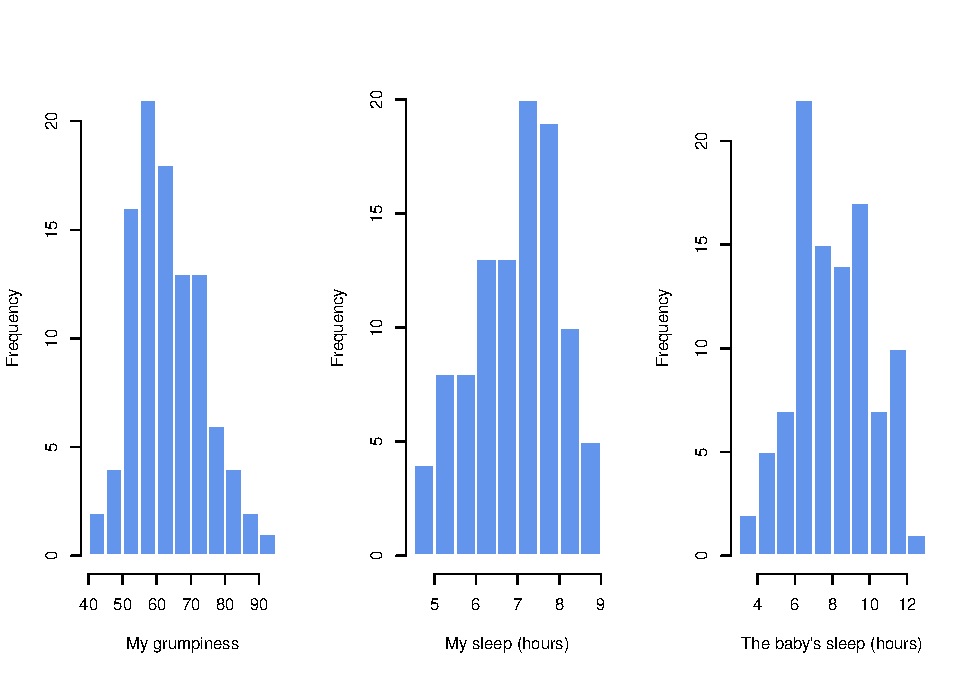
\includegraphics{navarro2_files/figure-latex/parenthood-1.pdf}
\caption{\label{fig:parenthood}Histograms for the three interesting
variables in the \texttt{parenthood} data set}
\end{figure}

One thing to note: just because R can calculate dozens of different
statistics doesn't mean you should report all of them. If I were writing
this up for a report, I'd probably pick out those statistics that are of
most interest to me (and to my readership), and then put them into a
nice, simple table like the one in Table \ref{tab:parenthood}.\footnote{Actually,
  even that table is more than I'd bother with. In practice most people
  pick \emph{one} measure of central tendency, and \emph{one} measure of
  variability only.} Notice that when I put it into a table, I gave
everything ``human readable'' names. This is always good practice.
Notice also that I'm not getting enough sleep. This isn't good practice,
but other parents tell me that it's standard practice.

\begin{table}

\caption{\label{tab:parenthoodtab}Descriptive statistics for the parenthood data.}
\centering
\begin{tabular}[t]{lllllll}
\toprule
variable & min & max & mean & median & std. dev & IQR\\
\midrule
Dan's grumpiness & 41 & 91 & 63.71 & 62 & 10.05 & 14\\
Dan's hours slept & 4.84 & 9 & 6.97 & 7.03 & 1.02 & 1.45\\
Dan's son's hours slept & 3.25 & 12.07 & 8.05 & 7.95 & 2.07 & 3.21\\
\bottomrule
\end{tabular}
\end{table}

\subsection{The strength and direction of a
relationship}\label{the-strength-and-direction-of-a-relationship}

\begin{figure}
\centering
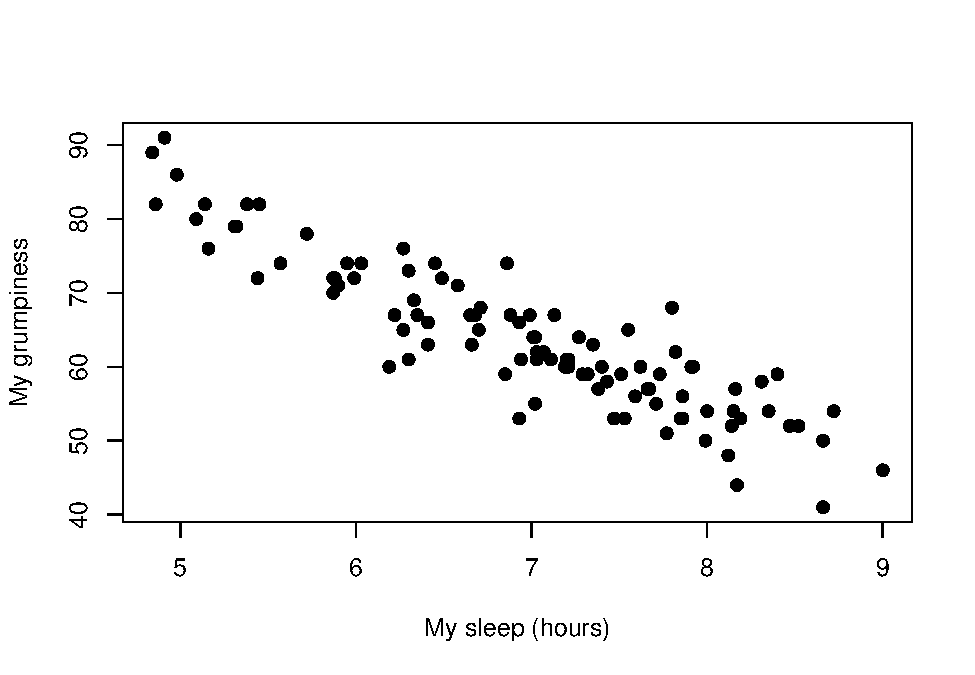
\includegraphics{navarro2_files/figure-latex/scatterparent1a-1.pdf}
\caption{\label{fig:scatterparent1a}Scatterplot showing the relationship
between \texttt{dan.sleep} and \texttt{dan.grump}}
\end{figure}

\begin{figure}
\centering
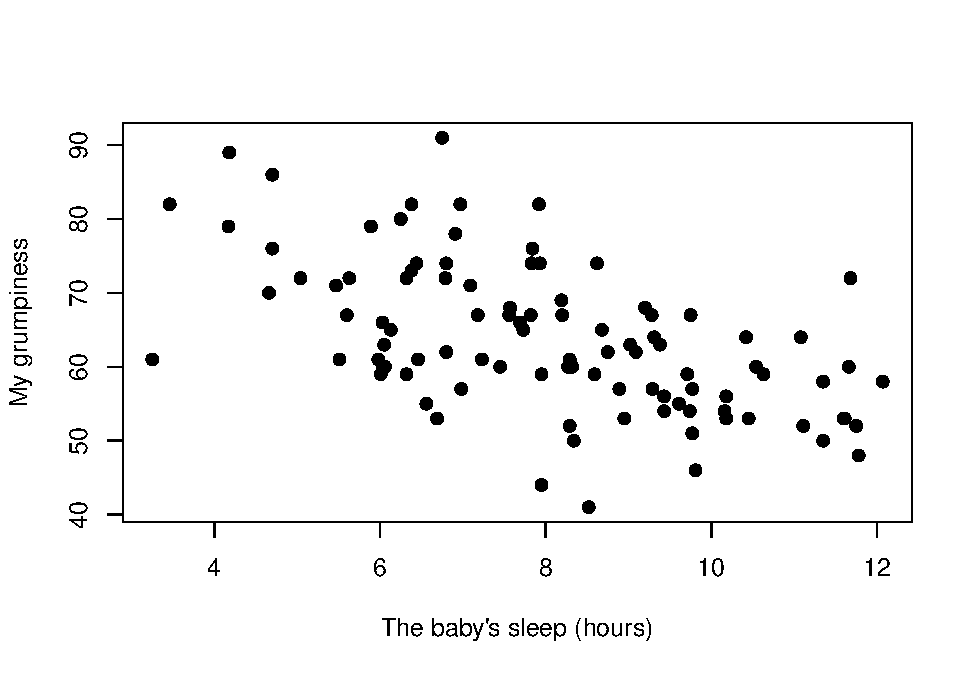
\includegraphics{navarro2_files/figure-latex/scatterparent1b-1.pdf}
\caption{\label{fig:scatterparent1b}Scatterplot showing the relationship
between \texttt{baby.sleep} and \texttt{dan.grump}}
\end{figure}

We can draw scatterplots to give us a general sense of how closely
related two variables are. Ideally though, we might want to say a bit
more about it than that. For instance, let's compare the relationship
between \texttt{dan.sleep} and \texttt{dan.grump} (Figure
\ref{fig:scatterparent1a} with that between \texttt{baby.sleep} and
\texttt{dan.grump} (Figure \ref{fig:scatterparent1b}. When looking at
these two plots side by side, it's clear that the relationship is
\emph{qualitatively} the same in both cases: more sleep equals less
grump! However, it's also pretty obvious that the relationship between
\texttt{dan.sleep} and \texttt{dan.grump} is \emph{stronger} than the
relationship between \texttt{baby.sleep} and \texttt{dan.grump}. The
plot on the left is ``neater'' than the one on the right. What it feels
like is that if you want to predict what my mood is, it'd help you a
little bit to know how many hours my son slept, but it'd be \emph{more}
helpful to know how many hours I slept.

In contrast, let's consider Figure \ref{fig:scatterparent1b} vs.~Figure
\ref{fig:scatterparent2}. If we compare the scatterplot of
``\texttt{baby.sleep} v \texttt{dan.grump}'' to the scatterplot of
```\texttt{baby.sleep} v \texttt{dan.sleep}'', the overall strength of
the relationship is the same, but the direction is different. That is,
if my son sleeps more, I get \emph{more} sleep (positive relationship,
but if he sleeps more then I get \emph{less} grumpy (negative
relationship).

\begin{figure}
\centering
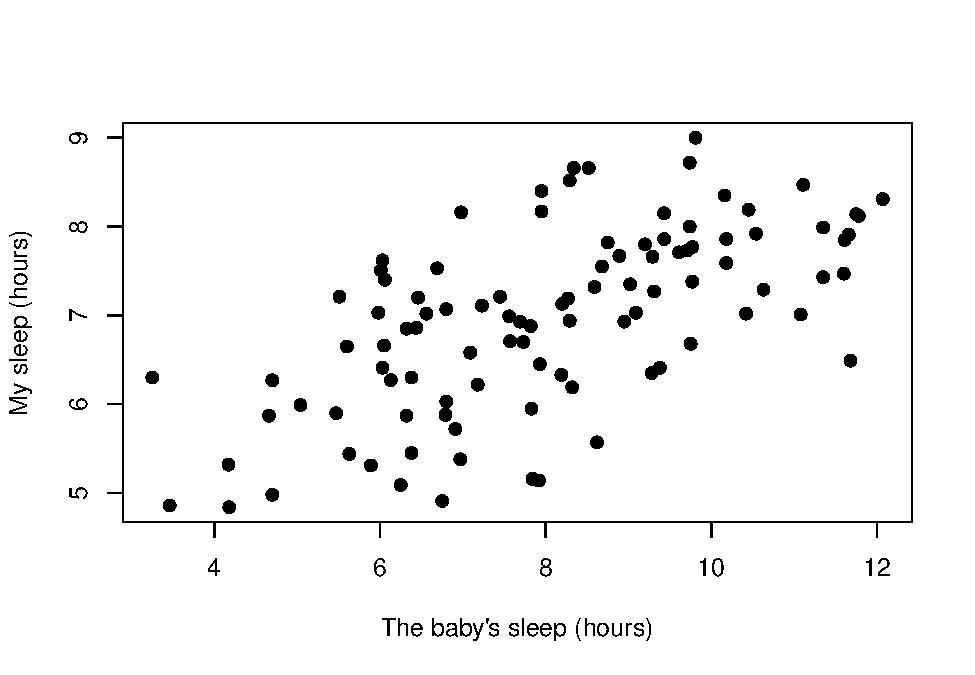
\includegraphics{navarro2_files/figure-latex/scatterparent2-1.pdf}
\caption{\label{fig:scatterparent2}Scatterplot showing the relationship
between \texttt{baby.sleep} and \texttt{dan.sleep}}
\end{figure}

\subsection{The correlation
coefficient}\label{the-correlation-coefficient}

We can make these ideas a bit more explicit by introducing the idea of a
\textbf{\emph{correlation coefficient}} (or, more specifically,
Pearson's correlation coefficient), which is traditionally denoted by
\(r\). The correlation coefficient between two variables \(X\) and \(Y\)
(sometimes denoted \(r_{XY}\)), which we'll define more precisely in the
next section, is a measure that varies from \(-1\) to \(1\). When
\(r = -1\) it means that we have a perfect negative relationship, and
when \(r = 1\) it means we have a perfect positive relationship. When
\(r = 0\), there's no relationship at all. If you look at Figure
\ref{fig:corr}, you can see several plots showing what different
correlations look like.

\begin{figure}
\centering
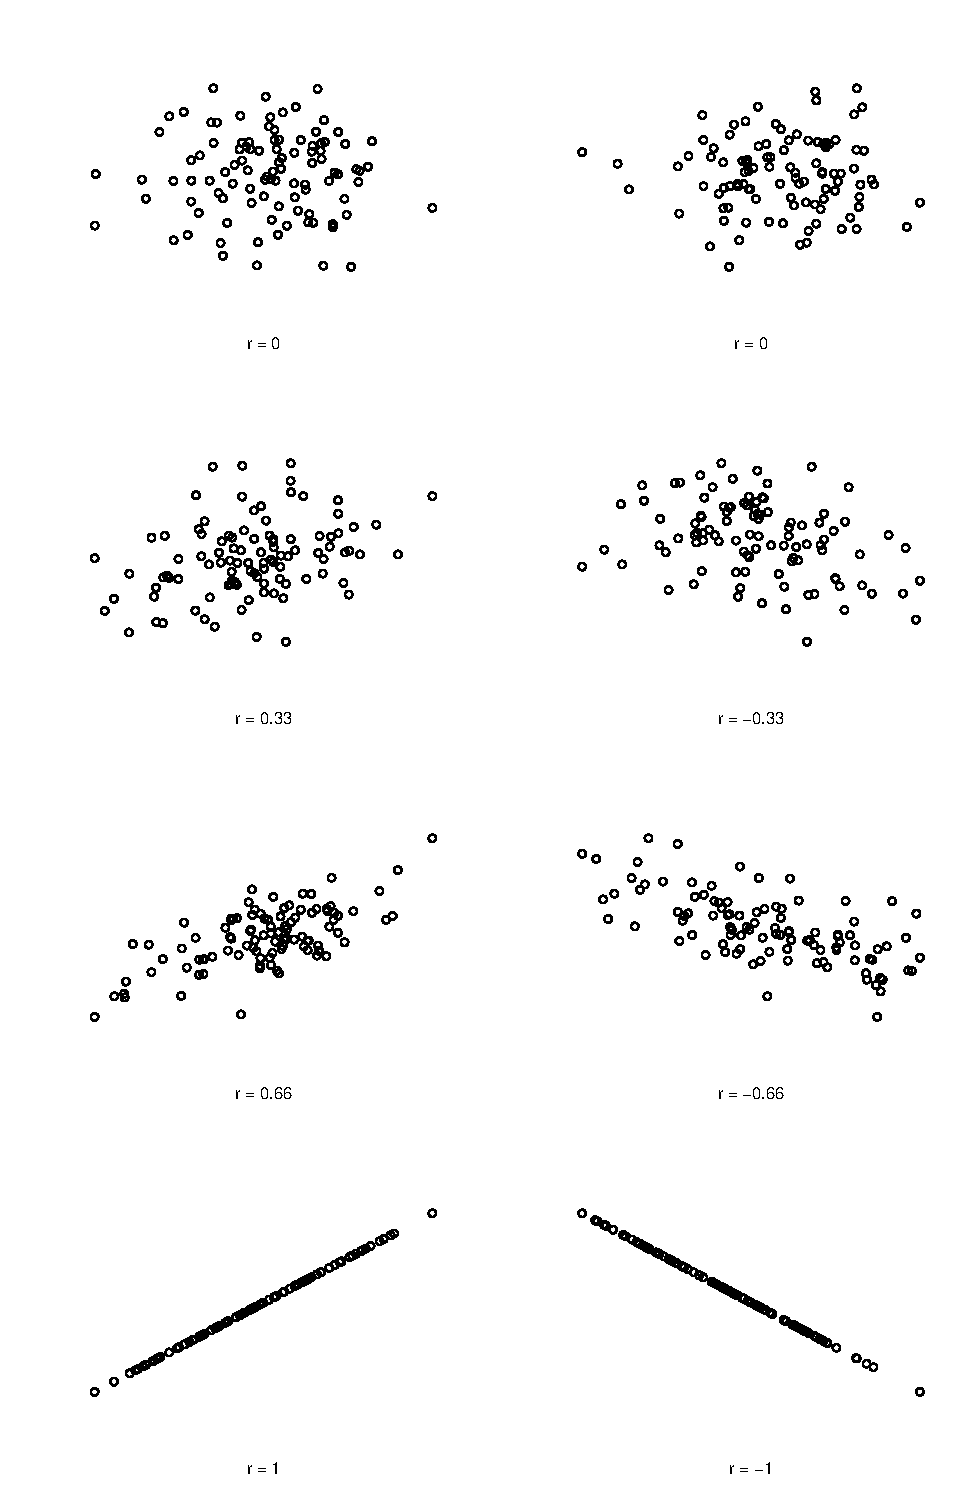
\includegraphics{navarro2_files/figure-latex/corr-1.pdf}
\caption{\label{fig:corr}Illustration of the effect of varying the strength
and direction of a correlation}
\end{figure}

The formula for the Pearson's correlation coefficient can be written in
several different ways. I think the simplest way to write down the
formula is to break it into two steps. Firstly, let's introduce the idea
of a \textbf{\emph{covariance}}. The covariance between two variables
\(X\) and \(Y\) is a generalisation of the notion of the variance; it's
a mathematically simple way of describing the relationship between two
variables that isn't terribly informative to humans: \[
\mbox{Cov}(X,Y) = \frac{1}{N-1} \sum_{i=1}^N \left( X_i - \bar{X} \right) \left( Y_i - \bar{Y} \right)
\] Because we're multiplying (i.e., taking the ``product'' of) a
quantity that depends on \(X\) by a quantity that depends on \(Y\) and
then averaging\footnote{Just like we saw with the variance and the
  standard deviation, in practice we divide by \(N-1\) rather than
  \(N\).}, you can think of the formula for the covariance as an
``average cross product'' between \(X\) and \(Y\). The covariance has
the nice property that, if \(X\) and \(Y\) are entirely unrelated, then
the covariance is exactly zero. If the relationship between them is
positive (in the sense shown in
\href{mailto:Figure@reffig}{\nolinkurl{Figure@reffig}}:corr) then the
covariance is also positive; and if the relationship is negative then
the covariance is also negative. In other words, the covariance captures
the basic qualitative idea of correlation. Unfortunately, the raw
magnitude of the covariance isn't easy to interpret: it depends on the
units in which \(X\) and \(Y\) are expressed, and worse yet, the actual
units that the covariance itself is expressed in are really weird. For
instance, if \(X\) refers to the \texttt{dan.sleep} variable (units:
hours) and \(Y\) refers to the \texttt{dan.grump} variable (units:
grumps), then the units for their covariance are ``hours \(\times\)
grumps''. And I have no freaking idea what that would even mean.

The Pearson correlation coefficient \(r\) fixes this interpretation
problem by standardising the covariance, in pretty much the exact same
way that the \(z\)-score standardises a raw score: by dividing by the
standard deviation. However, because we have two variables that
contribute to the covariance, the standardisation only works if we
divide by both standard deviations.\footnote{This is an
  oversimplification, but it'll do for our purposes.} In other words,
the correlation between \(X\) and \(Y\) can be written as follows: \[
r_{XY}  = \frac{\mbox{Cov}(X,Y)}{ \hat{\sigma}_X \ \hat{\sigma}_Y}
\] By doing this standardisation, not only do we keep all of the nice
properties of the covariance discussed earlier, but the actual values of
\(r\) are on a meaningful scale: \(r= 1\) implies a perfect positive
relationship, and \(r = -1\) implies a perfect negative relationship.
I'll expand a little more on this point later, in
\href{mailto:Section@refsec}{\nolinkurl{Section@refsec}}:interpretingcorrelations.
But before I do, let's look at how to calculate correlations in R.

\subsection{Calculating correlations in
R}\label{calculating-correlations-in-r}

Calculating correlations in R can be done using the \texttt{cor()}
command. The simplest way to use the command is to specify two input
arguments \texttt{x} and \texttt{y}, each one corresponding to one of
the variables. The following extract illustrates the basic usage of the
function:\footnote{If you are reading this after having already
  completed Chapter \ref{hypothesistesting} you might be wondering about
  hypothesis tests for correlations. R has a function called
  \texttt{cor.test()} that runs a hypothesis test for a single
  correlation, and the \texttt{psych} package contains a version called
  \texttt{corr.test()} that can run tests for every correlation in a
  correlation matrix; hypothesis tests for correlations are discussed in
  more detail in Section \ref{corrhyp}.}

\begin{Shaded}
\begin{Highlighting}[]
\KeywordTok{cor}\NormalTok{( }\DataTypeTok{x =}\NormalTok{ parenthood}\OperatorTok{$}\NormalTok{dan.sleep, }\DataTypeTok{y =}\NormalTok{ parenthood}\OperatorTok{$}\NormalTok{dan.grump )}
\end{Highlighting}
\end{Shaded}

\begin{verbatim}
## [1] -0.903384
\end{verbatim}

However, the \texttt{cor()} function is a bit more powerful than this
simple example suggests. For example, you can also calculate a complete
``correlation matrix'', between all pairs of variables in the data
frame:\footnote{An alternative usage of \texttt{cor()} is to correlate
  one set of variables with another subset of variables. If \texttt{X}
  and \texttt{Y} are both data frames with the same number of rows, then
  \texttt{cor(x\ =\ X,\ y\ =\ Y)} will produce a correlation matrix that
  correlates all variables in \texttt{X} with all variables in
  \texttt{Y}.}

\begin{Shaded}
\begin{Highlighting}[]
\CommentTok{# correlate all pairs of variables in "parenthood":}
\KeywordTok{cor}\NormalTok{( }\DataTypeTok{x =}\NormalTok{ parenthood )  }
\end{Highlighting}
\end{Shaded}

\begin{verbatim}
##              dan.sleep  baby.sleep   dan.grump         day
## dan.sleep   1.00000000  0.62794934 -0.90338404 -0.09840768
## baby.sleep  0.62794934  1.00000000 -0.56596373 -0.01043394
## dan.grump  -0.90338404 -0.56596373  1.00000000  0.07647926
## day        -0.09840768 -0.01043394  0.07647926  1.00000000
\end{verbatim}

\subsection{Interpreting a correlation}\label{interpretingcorrelations}

Naturally, in real life you don't see many correlations of 1. So how
should you interpret a correlation of, say \(r= .4\)? The honest answer
is that it really depends on what you want to use the data for, and on
how strong the correlations in your field tend to be. A friend of mine
in engineering once argued that any correlation less than \(.95\) is
completely useless (I think he was exaggerating, even for engineering).
On the other hand there are real cases -- even in psychology -- where
you should really expect correlations that strong. For instance, one of
the benchmark data sets used to test theories of how people judge
similarities is so clean that any theory that can't achieve a
correlation of at least \(.9\) really isn't deemed to be successful.
However, when looking for (say) elementary correlates of intelligence
(e.g., inspection time, response time), if you get a correlation above
\(.3\) you're doing very very well. In short, the interpretation of a
correlation depends a lot on the context. That said, the rough guide in
Table \ref{tab:interpretingcorrelations} is pretty typical.

\begin{Shaded}
\begin{Highlighting}[]
\NormalTok{knitr}\OperatorTok{::}\KeywordTok{kable}\NormalTok{(}
\KeywordTok{rbind}\NormalTok{(}
\KeywordTok{c}\NormalTok{(}\StringTok{"-1.0 to -0.9"}\NormalTok{ ,}\StringTok{"Very strong"}\NormalTok{, }\StringTok{"Negative"}\NormalTok{),}
\KeywordTok{c}\NormalTok{(}\StringTok{"-0.9 to -0.7"}\NormalTok{, }\StringTok{"Strong"}\NormalTok{, }\StringTok{"Negative"}\NormalTok{) ,}
\KeywordTok{c}\NormalTok{(}\StringTok{"-0.7 to -0.4"}\NormalTok{, }\StringTok{"Moderate"}\NormalTok{, }\StringTok{"Negative"}\NormalTok{) ,}
\KeywordTok{c}\NormalTok{(}\StringTok{"-0.4 to -0.2"}\NormalTok{, }\StringTok{"Weak"}\NormalTok{, }\StringTok{"Negative"}\NormalTok{),}
\KeywordTok{c}\NormalTok{(}\StringTok{"-0.2 to 0"}\NormalTok{,}\StringTok{"Negligible"}\NormalTok{, }\StringTok{"Negative"}\NormalTok{) ,}
\KeywordTok{c}\NormalTok{(}\StringTok{"0 to 0.2"}\NormalTok{,}\StringTok{"Negligible"}\NormalTok{, }\StringTok{"Positive"}\NormalTok{),}
\KeywordTok{c}\NormalTok{(}\StringTok{"0.2 to 0.4"}\NormalTok{, }\StringTok{"Weak"}\NormalTok{, }\StringTok{"Positive"}\NormalTok{), }
\KeywordTok{c}\NormalTok{(}\StringTok{"0.4 to 0.7"}\NormalTok{, }\StringTok{"Moderate"}\NormalTok{, }\StringTok{"Positive"}\NormalTok{), }
\KeywordTok{c}\NormalTok{(}\StringTok{"0.7 to 0.9"}\NormalTok{, }\StringTok{"Strong"}\NormalTok{, }\StringTok{"Positive"}\NormalTok{), }
\KeywordTok{c}\NormalTok{(}\StringTok{"0.9 to 1.0"}\NormalTok{, }\StringTok{"Very strong"}\NormalTok{, }\StringTok{"Positive"}\NormalTok{)), }\DataTypeTok{col.names=}\KeywordTok{c}\NormalTok{(}\StringTok{"Correlation"}\NormalTok{, }\StringTok{"Strength"}\NormalTok{, }\StringTok{"Direction"}\NormalTok{),}
  \DataTypeTok{booktabs =} \OtherTok{TRUE}\NormalTok{)}
\end{Highlighting}
\end{Shaded}

\begin{tabular}{lll}
\toprule
Correlation & Strength & Direction\\
\midrule
-1.0 to -0.9 & Very strong & Negative\\
-0.9 to -0.7 & Strong & Negative\\
-0.7 to -0.4 & Moderate & Negative\\
-0.4 to -0.2 & Weak & Negative\\
-0.2 to 0 & Negligible & Negative\\
\addlinespace
0 to 0.2 & Negligible & Positive\\
0.2 to 0.4 & Weak & Positive\\
0.4 to 0.7 & Moderate & Positive\\
0.7 to 0.9 & Strong & Positive\\
0.9 to 1.0 & Very strong & Positive\\
\bottomrule
\end{tabular}

However, something that can never be stressed enough is that you should
\emph{always} look at the scatterplot before attaching any
interpretation to the data. A correlation might not mean what you think
it means. The classic illustration of this is ``Anscombe's Quartet''
\citet[Anscombe1973]{ref}, which is a collection of four data sets. Each
data set has two variables, an \(X\) and a \(Y\). For all four data sets
the mean value for \(X\) is 9 and the mean for \(Y\) is 7.5. The,
standard deviations for all \(X\) variables are almost identical, as are
those for the the \(Y\) variables. And in each case the correlation
between \(X\) and \(Y\) is \(r = 0.816\). You can verify this yourself,
since the dataset comes distributed with R. The commands would be:

\begin{Shaded}
\begin{Highlighting}[]
\KeywordTok{cor}\NormalTok{( anscombe}\OperatorTok{$}\NormalTok{x1, anscombe}\OperatorTok{$}\NormalTok{y1 )}
\end{Highlighting}
\end{Shaded}

\begin{verbatim}
## [1] 0.8164205
\end{verbatim}

\begin{Shaded}
\begin{Highlighting}[]
\KeywordTok{cor}\NormalTok{( anscombe}\OperatorTok{$}\NormalTok{x2, anscombe}\OperatorTok{$}\NormalTok{y2 )}
\end{Highlighting}
\end{Shaded}

\begin{verbatim}
## [1] 0.8162365
\end{verbatim}

and so on.

You'd think that these four data setswould look pretty similar to one
another. They do not. If we draw scatterplots of \(X\) against \(Y\) for
all four variables, as shown in Figure \ref{fig:anscombe} we see that
all four of these are \emph{spectacularly} different to each other.
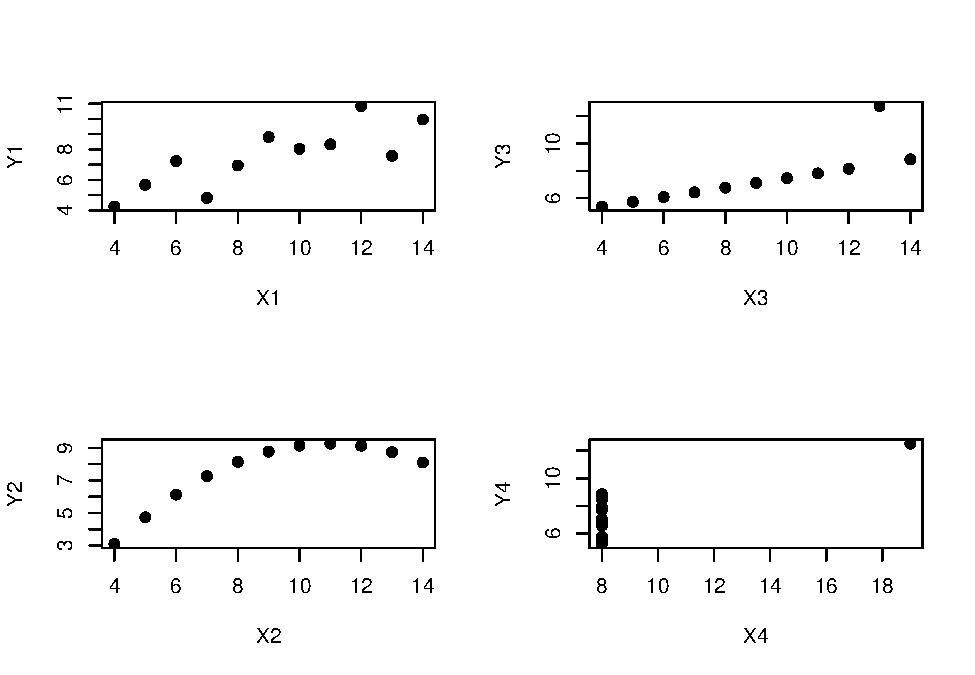
\includegraphics{navarro2_files/figure-latex/anscombe-1.pdf}

The lesson here, which so very many people seem to forget in real life
is ``\emph{always graph your raw data}''. This will be the focus of
Chapter \ref{graphics}.

\subsection{Spearman's rank
correlations}\label{spearmans-rank-correlations}

\begin{figure}
\centering
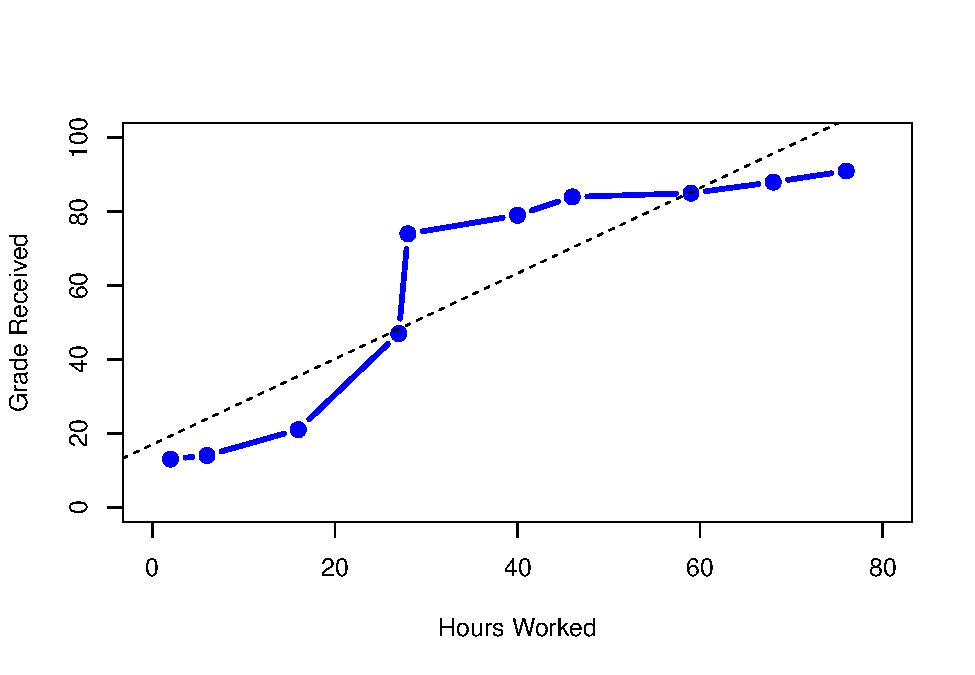
\includegraphics{navarro2_files/figure-latex/rankcorrpic-1.pdf}
\caption{\label{fig:rankcorrpic}The relationship between hours worked and
grade received, for a toy data set consisting of only 10 students (each
circle corresponds to one student). The dashed line through the middle
shows the linear relationship between the two variables. This produces a
strong Pearson correlation of \(r = .91\). However, the interesting
thing to note here is that there's actually a perfect monotonic
relationship between the two variables: in this toy example at least,
increasing the hours worked always increases the grade received, as
illustrated by the solid line. This is reflected in a Spearman
correlation of \(rho = 1\). With such a small data set, however, it's an
open question as to which version better describes the actual
relationship involved.}
\end{figure}

The Pearson correlation coefficient is useful for a lot of things, but
it does have shortcomings. One issue in particular stands out: what it
actually measures is the strength of the \emph{linear} relationship
between two variables. In other words, what it gives you is a measure of
the extent to which the data all tend to fall on a single, perfectly
straight line. Often, this is a pretty good approximation to what we
mean when we say ``relationship'', and so the Pearson correlation is a
good thing to calculation. Sometimes, it isn't.

One very common situation where the Pearson correlation isn't quite the
right thing to use arises when an increase in one variable \(X\) really
is reflected in an increase in another variable \(Y\), but the nature of
the relationship isn't necessarily linear. An example of this might be
the relationship between effort and reward when studying for an exam. If
you put in zero effort (\(X\)) into learning a subject, then you should
expect a grade of 0\% (\(Y\)). However, a little bit of effort will
cause a \emph{massive} improvement: just turning up to lectures means
that you learn a fair bit, and if you just turn up to classes, and
scribble a few things down so your grade might rise to 35\%, all without
a lot of effort. However, you just don't get the same effect at the
other end of the scale. As everyone knows, it takes \emph{a lot} more
effort to get a grade of 90\% than it takes to get a grade of 55\%. What
this means is that, if I've got data looking at study effort and grades,
there's a pretty good chance that Pearson correlations will be
misleading.

To illustrate, consider the data plotted in Figure
\ref{fig:rankcorrpic}, showing the relationship between hours worked and
grade received for 10 students taking some class. The curious thing
about this -- highly fictitious -- data set is that increasing your
effort \emph{always} increases your grade. It might be by a lot or it
might be by a little, but increasing effort will never decrease your
grade. The data are stored in \texttt{effort.Rdata}:

\begin{verbatim}
> load( "effort.Rdata" )
> who(TRUE)
   -- Name --   -- Class --   -- Size --
   effort       data.frame    10 x 2    
    $hours      numeric       10        
    $grade      numeric       10        
\end{verbatim}

The raw data look like this:

\begin{verbatim}
> effort
   hours grade
1      2    13
2     76    91
3     40    79
4      6    14
5     16    21
6     28    74
7     27    47
8     59    85
9     46    84
10    68    88
\end{verbatim}

If we run a standard Pearson correlation, it shows a strong relationship
between hours worked and grade received,

\begin{verbatim}
> cor( effort$hours, effort$grade )
[1] 0.909402
\end{verbatim}

but this doesn't actually capture the observation that increasing hours
worked \emph{always} increases the grade. There's a sense here in which
we want to be able to say that the correlation is \emph{perfect} but for
a somewhat different notion of what a ``relationship'' is. What we're
looking for is something that captures the fact that there is a perfect
\textbf{\emph{ordinal relationship}} here. That is, if student 1 works
more hours than student 2, then we can guarantee that student 1 will get
the better grade. That's not what a correlation of \(r = .91\) says at
all.

How should we address this? Actually, it's really easy: if we're looking
for ordinal relationships, all we have to do is treat the data as if it
were ordinal scale! So, instead of measuring effort in terms of ``hours
worked'', lets rank all 10 of our students in order of hours worked.
That is, student 1 did the least work out of anyone (2 hours) so they
get the lowest rank (rank = 1). Student 4 was the next laziest, putting
in only 6 hours of work in over the whole semester, so they get the next
lowest rank (rank = 2). Notice that I'm using ``rank =1'' to mean ``low
rank''. Sometimes in everyday language we talk about ``rank = 1'' to
mean ``top rank'' rather than ``bottom rank''. So be careful: you can
rank ``from smallest value to largest value'' (i.e., small equals rank
1) or you can rank ``from largest value to smallest value'' (i.e., large
equals rank 1). In this case, I'm ranking from smallest to largest,
because that's the default way that R does it. But in real life, it's
really easy to forget which way you set things up, so you have to put a
bit of effort into remembering!

Okay, so let's have a look at our students when we rank them from worst
to best in terms of effort and reward:

\begin{longtable}[]{@{}lll@{}}
\toprule
& rank (hours worked) & rank (grade received)\tabularnewline
\midrule
\endhead
student & 1 & 1\tabularnewline
student & 2 & 10\tabularnewline
student & 3 & 6\tabularnewline
student & 4 & 2\tabularnewline
student & 5 & 3\tabularnewline
student & 6 & 5\tabularnewline
student & 7 & 4\tabularnewline
student & 8 & 8\tabularnewline
student & 9 & 7\tabularnewline
student & 10 & 9\tabularnewline
\bottomrule
\end{longtable}

Hm. These are \emph{identical}. The student who put in the most effort
got the best grade, the student with the least effort got the worst
grade, etc. We can get R to construct these rankings using the
\texttt{rank()} function, like this:

\begin{verbatim}
> hours.rank <- rank( effort$hours )   # rank students by hours worked
> grade.rank <- rank( effort$grade )   # rank students by grade received
\end{verbatim}

As the table above shows, these two rankings are identical, so if we now
correlate them we get a perfect relationship:

\begin{verbatim}
> cor( hours.rank, grade.rank )
[1] 1
\end{verbatim}

What we've just re-invented is \textbf{\emph{Spearman's rank order
correlation}}, usually denoted \(\rho\) to distinguish it from the
Pearson correlation \(r\). We can calculate Spearman's \(\rho\) using R
in two different ways. Firstly we could do it the way I just showed,
using the \texttt{rank()} function to construct the rankings, and then
calculate the Pearson correlation on these ranks. However, that's way
too much effort to do every time. It's much easier to just specify the
\texttt{method} argument of the \texttt{cor()} function.

\begin{verbatim}
> cor( effort$hours, effort$grade, method = "spearman")
[1] 1
\end{verbatim}

The default value of the \texttt{method} argument is \texttt{"pearson"},
which is why we didn't have to specify it earlier on when we were doing
Pearson correlations.

\subsection{\texorpdfstring{The \texttt{correlate()}
function}{The correlate() function}}\label{the-correlate-function}

As we've seen, the \texttt{cor()} function works pretty well, and
handles many of the situations that you might be interested in. One
thing that many beginners find frustrating, however, is the fact that
it's not built to handle non-numeric variables. From a statistical
perspective, this is perfectly sensible: Pearson and Spearman
correlations are only designed to work for numeric variables, so the
\texttt{cor()} function spits out an error.

Here's what I mean. Suppose you were keeping track of how many
\texttt{hours} you worked in any given day, and counted how many
\texttt{tasks} you completed. If you were doing the tasks for money, you
might also want to keep track of how much \texttt{pay} you got for each
job. It would also be sensible to keep track of the \texttt{weekday} on
which you actually did the work: most of us don't work as much on
Saturdays or Sundays. If you did this for 7 weeks, you might end up with
a data set that looks like this one:

\begin{verbatim}
> load("work.Rdata")

> who(TRUE)
   -- Name --   -- Class --   -- Size --
   work         data.frame    49 x 7    
    $hours      numeric       49        
    $tasks      numeric       49        
    $pay        numeric       49        
    $day        integer       49        
    $weekday    factor        49        
    $week       numeric       49        
    $day.type   factor        49   
    
> head(work)
  hours tasks pay day   weekday week day.type
1   7.2    14  41   1   Tuesday    1  weekday
2   7.4    11  39   2 Wednesday    1  weekday
3   6.6    14  13   3  Thursday    1  weekday
4   6.5    22  47   4    Friday    1  weekday
5   3.1     5   4   5  Saturday    1  weekend
6   3.0     7  12   6    Sunday    1  weekend
\end{verbatim}

Obviously, I'd like to know something about how all these variables
correlate with one another. I could correlate \texttt{hours} with
\texttt{pay} quite using \texttt{cor()}, like so:

\begin{verbatim}
> cor(work$hours,work$pay)
[1] 0.7604283
\end{verbatim}

But what if I wanted a quick and easy way to calculate all pairwise
correlations between the numeric variables? I can't just input the
\texttt{work} data frame, because it contains two factor variables,
\texttt{weekday} and \texttt{day.type}. If I try this, I get an error:

\begin{verbatim}
> cor(work)
Error in cor(work) : 'x' must be numeric
\end{verbatim}

It order to get the correlations that I want using the \texttt{cor()}
function, is create a new data frame that doesn't contain the factor
variables, and then feed that new data frame into the \texttt{cor()}
function. It's not actually very hard to do that, and I'll talk about
how to do it properly in
\href{mailto:Section@refsec}{\nolinkurl{Section@refsec}}:subsetdataframe.
But it would be nice to have some function that is smart enough to just
ignore the factor variables. That's where the \texttt{correlate()}
function in the \texttt{lsr} package can be handy. If you feed it a data
frame that contains factors, it knows to ignore them, and returns the
pairwise correlations only between the numeric variables:

\begin{verbatim}
> correlate(work)

CORRELATIONS
============
- correlation type:  pearson 
- correlations shown only when both variables are numeric

          hours  tasks   pay    day weekday   week day.type
hours         .  0.800 0.760 -0.049       .  0.018        .
tasks     0.800      . 0.720 -0.072       . -0.013        .
pay       0.760  0.720     .  0.137       .  0.196        .
day      -0.049 -0.072 0.137      .       .  0.990        .
weekday       .      .     .      .       .      .        .
week      0.018 -0.013 0.196  0.990       .      .        .
day.type      .      .     .      .       .      .        .
\end{verbatim}

The output here shows a \texttt{.} whenever one of the variables is
non-numeric. It also shows a \texttt{.} whenever a variable is
correlated with itself (it's not a meaningful thing to do). The
\texttt{correlate()} function can also do Spearman correlations, by
specifying the \texttt{corr.method} to use:

\begin{verbatim}
> correlate( work, corr.method="spearman" )

CORRELATIONS
============
- correlation type:  spearman 
- correlations shown only when both variables are numeric

          hours  tasks   pay    day weekday   week day.type
hours         .  0.805 0.745 -0.047       .  0.010        .
tasks     0.805      . 0.730 -0.068       . -0.008        .
pay       0.745  0.730     .  0.094       .  0.154        .
day      -0.047 -0.068 0.094      .       .  0.990        .
weekday       .      .     .      .       .      .        .
week      0.010 -0.008 0.154  0.990       .      .        .
day.type      .      .     .      .       .      .        .
\end{verbatim}

Obviously, there's no new functionality in the \texttt{correlate()}
function, and any advanced R user would be perfectly capable of using
the \texttt{cor()} function to get these numbers out. But if you're not
yet comfortable with extracting a subset of a data frame, the
\texttt{correlate()} function is for you.

\section{Handling missing values}\label{missing}

There's one last topic that I want to discuss briefly in this chapter,
and that's the issue of \textbf{\emph{missing data}}. Real data sets
very frequently turn out to have missing values: perhaps someone forgot
to fill in a particular survey question, for instance. Missing data can
be the source of a lot of tricky issues, most of which I'm going to
gloss over. However, at a minimum, you need to understand the basics of
handling missing data in R.

\subsection{The single variable case}\label{the-single-variable-case}

Let's start with the simplest case, in which you're trying to calculate
descriptive statistics for a single variable which has missing data. In
R, this means that there will be \texttt{NA} values in your data vector.
Let's create a variable like that:

\begin{verbatim}
> partial <- c(10, 20, NA, 30)
\end{verbatim}

Let's assume that you want to calculate the mean of this variable. By
default, R assumes that you want to calculate the mean using all four
elements of this vector, which is probably the safest thing for a dumb
automaton to do, but it's rarely what you actually want. Why not? Well,
remember that the basic interpretation of \texttt{NA} is ``I don't know
what this number is''. This means that \texttt{1\ +\ NA\ =\ NA}: if I
add 1 to some number that I don't know (i.e., the \texttt{NA}) then the
answer is \emph{also} a number that I don't know. As a consequence, if
you don't explicitly tell R to ignore the \texttt{NA} values, and the
data set does have missing values, then the output will itself be a
missing value. If I try to calculate the mean of the \texttt{partial}
vector, without doing anything about the missing value, here's what
happens:

\begin{verbatim}
> mean( x = partial )
[1] NA
\end{verbatim}

Technically correct, but deeply unhelpful.

To fix this, all of the descriptive statistics functions that I've
discussed in this chapter (with the exception of \texttt{cor()} which is
a special case I'll discuss below) have an optional argument called
\texttt{na.rm}, which is shorthand for ``remove NA values''. By default,
\texttt{na.rm\ =\ FALSE}, so R does nothing about the missing data
problem. Let's try setting \texttt{na.rm\ =\ TRUE} and see what happens:

When calculating sums and means when missing data are present (i.e.,
when there are \texttt{NA} values) there's actually an additional
argument to the function that you should be aware of. This argument is
called \texttt{na.rm}, and is a logical value indicating whether R
should ignore (or ``remove'') the missing data for the purposes of doing
the calculations. By default, R assumes that you want to keep the
missing values, so unless you say otherwise it will set
\texttt{na.rm\ =\ FALSE}. However, R assumes that
\texttt{1\ +\ NA\ =\ NA}: if I add 1 to some number that I don't know
(i.e., the \texttt{NA}) then the answer is \emph{also} a number that I
don't know. As a consequence, if you don't explicitly tell R to ignore
the \texttt{NA} values, and the data set does have missing values, then
the output will itself be a missing value. This is illustrated in the
following extract:

\begin{verbatim}
> mean( x = partial, na.rm = TRUE )
[1] 20
\end{verbatim}

Notice that the mean is \texttt{20} (i.e., \texttt{60\ /\ 3}) and
\emph{not} \texttt{15}. When R ignores a \texttt{NA} value, it genuinely
ignores it. In effect, the calculation above is identical to what you'd
get if you asked for the mean of the three-element vector
\texttt{c(10,\ 20,\ 30)}.

As indicated above, this isn't unique to the \texttt{mean()} function.
Pretty much all of the other functions that I've talked about in this
chapter have an \texttt{na.rm} argument that indicates whether it should
ignore missing values. However, its behaviour is the same for all these
functions, so I won't waste everyone's time by demonstrating it
separately for each one.

\subsection{Missing values in pairwise
calculations}\label{missing-values-in-pairwise-calculations}

I mentioned earlier that the \texttt{cor()} function is a special case.
It doesn't have an \texttt{na.rm} argument, because the story becomes a
lot more complicated when more than one variable is involved. What it
does have is an argument called \texttt{use} which does roughly the same
thing, but you need to think little more carefully about what you want
this time. To illustrate the issues, let's open up a data set that has
missing values, \texttt{parenthood2.Rdata}. This file contains the same
data as the original parenthood data, but with some values deleted. It
contains a single data frame, \texttt{parenthood2}:

\begin{verbatim}
> load( "parenthood2.Rdata" )
> print( parenthood2 )
  dan.sleep baby.sleep dan.grump day
1      7.59         NA        56   1
2      7.91      11.66        60   2
3      5.14       7.92        82   3
4      7.71       9.61        55   4
5      6.68       9.75        NA   5
6      5.99       5.04        72   6
BLAH BLAH BLAH
\end{verbatim}

If I calculate my descriptive statistics using the \texttt{describe()}
function

\begin{verbatim}
> describe( parenthood2 )
           var   n  mean    sd median trimmed   mad   min    max    BLAH
dan.sleep    1  91  6.98  1.02   7.03    7.02  1.13  4.84   9.00    BLAH
baby.sleep   2  89  8.11  2.05   8.20    8.13  2.28  3.25  12.07    BLAH
dan.grump    3  92 63.15  9.85  61.00   62.66 10.38 41.00  89.00    BLAH
day          4 100 50.50 29.01  50.50   50.50 37.06  1.00 100.00    BLAH
\end{verbatim}

we can see from the \texttt{n} column that there are 9 missing values
for \texttt{dan.sleep}, 11 missing values for \texttt{baby.sleep} and 8
missing values for \texttt{dan.grump}.\footnote{It's worth noting that,
  even though we have missing data for each of these variables, the
  output doesn't contain any \texttt{NA} values. This is because, while
  \texttt{describe()} also has an \texttt{na.rm} argument, the default
  value for this function is \texttt{na.rm\ =\ TRUE}.} Suppose what I
would like is a correlation matrix. And let's also suppose that I don't
bother to tell R how to handle those missing values. Here's what
happens:

\begin{verbatim}
> cor( parenthood2 )
           dan.sleep baby.sleep dan.grump day
dan.sleep          1         NA        NA  NA
baby.sleep        NA          1        NA  NA
dan.grump         NA         NA         1  NA
day               NA         NA        NA   1
\end{verbatim}

Annoying, but it kind of makes sense. If I don't \emph{know} what some
of the values of \texttt{dan.sleep} and \texttt{baby.sleep} actually
are, then I can't possibly \emph{know} what the correlation between
these two variables is either, since the formula for the correlation
coefficient makes use of every single observation in the data set. Once
again, it makes sense: it's just not particularly \emph{helpful}.

To make R behave more sensibly in this situation, you need to specify
the \texttt{use} argument to the \texttt{cor()} function. There are
several different values that you can specify for this, but the two that
we care most about in practice tend to be \texttt{"complete.obs"} and
\texttt{"pairwise.complete.obs"}. If we specify
\texttt{use\ =\ "complete.obs"}, R will completely ignore all cases
(i.e., all rows in our \texttt{parenthood2} data frame) that have any
missing values at all. So, for instance, if you look back at the extract
earlier when I used the \texttt{head()} function, notice that
observation 1 (i.e., day 1) of the \texttt{parenthood2} data set is
missing the value for \texttt{baby.sleep}, but is otherwise complete?
Well, if you choose \texttt{use\ =\ "complete.obs"} R will ignore that
row completely: that is, even when it's trying to calculate the
correlation between \texttt{dan.sleep} and \texttt{dan.grump},
observation 1 will be ignored, because the value of \texttt{baby.sleep}
is missing for that observation. Here's what we get:

\begin{verbatim}
> cor(parenthood2, use = "complete.obs")
             dan.sleep baby.sleep   dan.grump         day
dan.sleep   1.00000000  0.6394985 -0.89951468  0.06132891
baby.sleep  0.63949845  1.0000000 -0.58656066  0.14555814
dan.grump  -0.89951468 -0.5865607  1.00000000 -0.06816586
day         0.06132891  0.1455581 -0.06816586  1.00000000
\end{verbatim}

The other possibility that we care about, and the one that tends to get
used more often in practice, is to set
\texttt{use\ =\ "pairwise.complete.obs"}. When we do that, R only looks
at the variables that it's trying to correlate when determining what to
drop. So, for instance, since the only missing value for observation 1
of \texttt{parenthood2} is for \texttt{baby.sleep} R will only drop
observation 1 when \texttt{baby.sleep} is one of the variables involved:
and so R keeps observation 1 when trying to correlate \texttt{dan.sleep}
and \texttt{dan.grump}. When we do it this way, here's what we get:

\begin{verbatim}
> cor(parenthood2, use = "pairwise.complete.obs") 
             dan.sleep  baby.sleep    dan.grump          day
dan.sleep   1.00000000  0.61472303 -0.903442442 -0.076796665
baby.sleep  0.61472303  1.00000000 -0.567802669  0.058309485
dan.grump  -0.90344244 -0.56780267  1.000000000  0.005833399
day        -0.07679667  0.05830949  0.005833399  1.000000000
\end{verbatim}

Similar, but not quite the same. It's also worth noting that the
\texttt{correlate()} function (in the \texttt{lsr} package)
automatically uses the ``pairwise complete'' method:

\begin{verbatim}
> correlate(parenthood2)

CORRELATIONS
============
- correlation type:  pearson 
- correlations shown only when both variables are numeric

           dan.sleep baby.sleep dan.grump    day
dan.sleep          .      0.615    -0.903 -0.077
baby.sleep     0.615          .    -0.568  0.058
dan.grump     -0.903     -0.568         .  0.006
day           -0.077      0.058     0.006      .
\end{verbatim}

The two approaches have different strengths and weaknesses. The
``pairwise complete'' approach has the advantage that it keeps more
observations, so you're making use of more of your data and (as we'll
discuss in tedious detail in Chapter \ref{estimation} and it improves
the reliability of your estimated correlation. On the other hand, it
means that every correlation in your correlation matrix is being
computed from a slightly different set of observations, which can be
awkward when you want to compare the different correlations that you've
got.

So which method should you use? It depends a lot on \emph{why} you think
your values are missing, and probably depends a little on how paranoid
you are. For instance, if you think that the missing values were
``chosen'' completely randomly\footnote{The technical term here is
  ``missing completely at random'' (often written MCAR for short). Makes
  sense, I suppose, but it does sound ungrammatical to me.} then you'll
probably want to use the pairwise method. If you think that missing data
are a cue to thinking that the whole observation might be rubbish (e.g.,
someone just selecting arbitrary responses in your questionnaire), but
that there's no pattern to which observations are ``rubbish'' then it's
probably safer to keep only those observations that are complete. If you
think there's something systematic going on, in that some observations
are more likely to be missing than others, then you have a much trickier
problem to solve, and one that is beyond the scope of this book.

\section{Summary}\label{summary-3}

Calculating some basic descriptive statistics is one of the very first
things you do when analysing real data, and descriptive statistics are
much simpler to understand than inferential statistics, so like every
other statistics textbook I've started with descriptives. In this
chapter, we talked about the following topics:

\begin{itemize}
\tightlist
\item
  \emph{Measures of central tendency}. Broadly speaking, central
  tendency measures tell you where the data are. There's three measures
  that are typically reported in the literature: the mean, median and
  mode. (Section \ref{centraltendency})
\item
  \emph{Measures of variability}. In contrast, measures of variability
  tell you about how ``spread out'' the data are. The key measures are:
  range, standard deviation, interquartile reange (Section \ref{var})
\item
  \emph{Getting summaries of variables in R}. Since this book focuses on
  doing data analysis in R, we spent a bit of time talking about how
  descriptive statistics are computed in R. (Section \ref{summary} and
  \ref{groupdescriptives})
\item
  \emph{Standard scores}. The \(z\)-score is a slightly unusual beast.
  It's not quite a descriptive statistic, and not quite an inference. We
  talked about it in Section \ref{zscore}. Make sure you understand that
  section: it'll come up again later.
\item
  \emph{Correlations}. Want to know how strong the relationship is
  between two variables? Calculate a correlation. (Section \ref{correl})
\item
  \emph{Missing data}. Dealing with missing data is one of those
  frustrating things that data analysts really wish the didn't have to
  think about. In real life it can be hard to do well. For the purpose
  of this book, we only touched on the basics in Section \ref{missing}
\end{itemize}

In the next section we'll move on to a discussion of how to draw
pictures! Everyone loves a pretty picture, right? But before we do, I
want to end on an important point. A traditional first course in
statistics spends only a small proportion of the class on descriptive
statistics, maybe one or two lectures at most. The vast majority of the
lecturer's time is spent on inferential statistics, because that's where
all the hard stuff is. That makes sense, but it hides the practical
everyday importance of choosing good descriptives. With that in
mind\ldots{}

\section{Epilogue: Good descriptive statistics are
descriptive!}\label{epilogue-good-descriptive-statistics-are-descriptive}

\begin{quote}
\emph{The death of one man is a tragedy. The death of millions is a
statistic.}

-- Josef Stalin, Potsdam 1945
\end{quote}

\begin{quote}
\emph{950,000 -- 1,200,000}

-- Estimate of Soviet repression deaths, 1937-1938 \citep{Ellman2002}
\end{quote}

Stalin's infamous quote about the statistical character death of
millions is worth giving some thought. The clear intent of his statement
is that the death of an individual touches us personally and its force
cannot be denied, but that the deaths of a multitude are
incomprehensible, and as a consequence mere statistics, more easily
ignored. I'd argue that Stalin was half right. A statistic is an
abstraction, a description of events beyond our personal experience, and
so hard to visualise. Few if any of us can imagine what the deaths of
millions is ``really'' like, but we can imagine one death, and this
gives the lone death its feeling of immediate tragedy, a feeling that is
missing from Ellman's cold statistical description.

Yet it is not so simple: without numbers, without counts, without a
description of what happened, we have \emph{no chance} of understanding
what really happened, no opportunity event to try to summon the missing
feeling. And in truth, as I write this, sitting in comfort on a Saturday
morning, half a world and a whole lifetime away from the Gulags, when I
put the Ellman estimate next to the Stalin quote a dull dread settles in
my stomach and a chill settles over me. The Stalinist repression is
something truly beyond my experience, but with a combination of
statistical data and those recorded personal histories that have come
down to us, it is not entirely beyond my comprehension. Because what
Ellman's numbers tell us is this: over a two year period, Stalinist
repression wiped out the equivalent of every man, woman and child
currently alive in the city where I live. Each one of those deaths had
it's own story, was it's own tragedy, and only some of those are known
to us now. Even so, with a few carefully chosen statistics, the scale of
the atrocity starts to come into focus.

Thus it is no small thing to say that the first task of the statistician
and the scientist is to summarise the data, to find some collection of
numbers that can convey to an audience a sense of what has happened.
This is the job of descriptive statistics, but it's not a job that can
be told solely using the numbers. You are a data analyst, not a
statistical software package. Part of your job is to take these
\emph{statistics} and turn them into a \emph{description}. When you
analyse data, it is not sufficient to list off a collection of numbers.
Always remember that what you're really trying to do is communicate with
a human audience. The numbers are important, but they need to be put
together into a meaningful story that your audience can interpret. That
means you need to think about framing. You need to think about context.
And you need to think about the individual events that your statistics
are summarising.

\chapter{Drawing graphs}\label{graphics}

\begin{quote}
\emph{Above all else show the data.}

--Edward Tufte\footnote{The origin of this quote is Tufte's lovely book
  \emph{The Visual Display of Quantitative Information}.}
\end{quote}

Visualising data is one of the most important tasks facing the data
analyst. It's important for two distinct but closely related reasons.
Firstly, there's the matter of drawing ``presentation graphics'':
displaying your data in a clean, visually appealing fashion makes it
easier for your reader to understand what you're trying to tell them.
Equally important, perhaps even more important, is the fact that drawing
graphs helps \emph{you} to understand the data. To that end, it's
important to draw ``exploratory graphics'' that help you learn about the
data as you go about analysing it. These points might seem pretty
obvious, but I cannot count the number of times I've seen people forget
them.

\begin{figure}
\centering
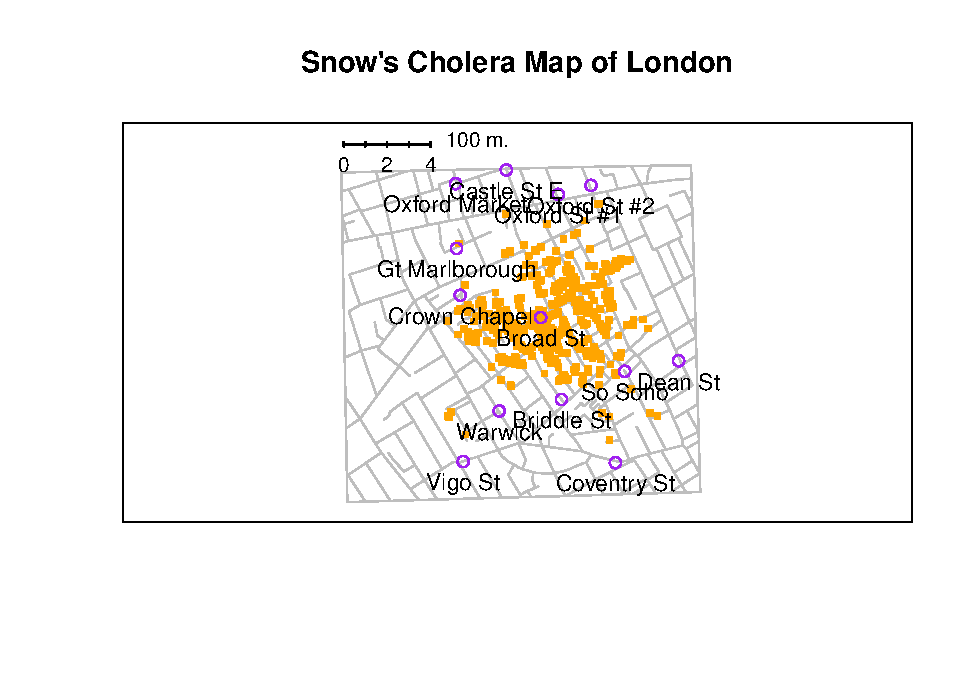
\includegraphics{navarro2_files/figure-latex/snowmap1-1.pdf}
\caption{\label{fig:snowmap1}A stylised redrawing of John Snow's original
cholera map. Each small dot represents the location of a cholera case,
and each large circle shows the location of a well. As the plot makes
clear, the cholera outbreak is centred very closely on the Broad St
pump. This image uses the data from the \texttt{HistData} package
@{[}Friendly2011{]}, and was drawn using minor alterations to the
commands provided in the help files. Note that Snow's original hand
drawn map used different symbols and labels, but you get the idea.}
\end{figure}

To give a sense of the importance of this chapter, I want to start with
a classic illustration of just how powerful a good graph can be. To that
end, Figure \ref{fig:snowmap1} shows a redrawing of one of the most
famous data visualisations of all time: John Snow's 1854 map of cholera
deaths. The map is elegant in its simplicity. In the background we have
a street map, which helps orient the viewer. Over the top, we see a
large number of small dots, each one representing the location of a
cholera case. The larger symbols show the location of water pumps,
labelled by name. Even the most casual inspection of the graph makes it
very clear that the source of the outbreak is almost certainly the Broad
Street pump. Upon viewing this graph, Dr Snow arranged to have the
handle removed from the pump, ending the outbreak that had killed over
500 people. Such is the power of a good data visualisation.

The goals in this chapter are twofold: firstly, to discuss several
fairly standard graphs that we use a lot when analysing and presenting
data, and secondly, to show you how to create these graphs in R. The
graphs themselves tend to be pretty straightforward, so in that respect
this chapter is pretty simple. Where people usually struggle is learning
how to produce graphs, and especially, learning how to produce good
graphs.\footnote{I should add that this isn't unique to R. Like
  everything in R there's a pretty steep learning curve to learning how
  to draw graphs, and like always there's a massive payoff at the end in
  terms of the quality of what you can produce. But to be honest, I've
  seen the same problems show up regardless of what system people use. I
  suspect that the hardest thing to do is to force yourself to take the
  time to think deeply about what your graphs are doing. I say that in
  full knowledge that only about half of my graphs turn out as well as
  they ought to. Understanding what makes a good graph is easy: actually
  designing a good graph is \emph{hard}.} Fortunately, learning how to
draw graphs in R is reasonably simple, as long as you're not too picky
about what your graph looks like. What I mean when I say this is that R
has a lot of \emph{very} good graphing functions, and most of the time
you can produce a clean, high-quality graphic without having to learn
very much about the low-level details of how R handles graphics.
Unfortunately, on those occasions when you do want to do something
non-standard, or if you need to make highly specific changes to the
figure, you actually do need to learn a fair bit about the these
details; and those details are both complicated and boring. With that in
mind, the structure of this chapter is as follows: I'll start out by
giving you a very quick overview of how graphics work in R. I'll then
discuss several different kinds of graph and how to draw them, as well
as showing the basics of how to customise these plots. I'll then talk in
more detail about R graphics, discussing some of those complicated and
boring issues. In a future version of this book, I intend to finish this
chapter off by talking about what makes a good or a bad graph, but I
haven't yet had the time to write that section.

\section{An overview of R graphics}\label{rgraphics}

Reduced to its simplest form, you can think of an R graphic as being
much like a painting. You start out with an empty canvas. Every time you
use a graphics function, it paints some new things onto your canvas.
Later on, you can paint more things over the top if you want; but just
like painting, you can't ``undo'' your strokes. If you make a mistake,
you have to throw away your painting and start over. Fortunately, this
is way more easy to do when using R than it is when painting a picture
in real life: you delete the plot and then type a new set of
commands.\footnote{Or, since you can always use the up and down keys to
  scroll through your recent command history, you can just pull up your
  most recent commands and edit them to fix your mistake. It becomes
  even easier once you start using scripts (Section \ref{scripts}, since
  all you have to do is edit your script and then run it again.} This
way of thinking about drawing graphs is referred to as the
\textbf{\emph{painter's model}}. So far, this probably doesn't sound
particularly complicated, and for the vast majority of graphs you'll
want to draw it's exactly as simple as it sounds. Much like painting in
real life, the headaches usually start when we dig into details. To see
why, I'll expand this ``painting metaphor'' a bit further just to show
you the basics of what's going on under the hood, but before I do I want
to stress that you really don't need to understand all these
complexities in order to draw graphs. I'd been using R for years before
I even realised that most of these issues existed! However, I don't want
you to go through the same pain I went through every time I
inadvertently discovered one of these things, so here's a quick
overview.

Firstly, if you want to paint a picture, you need to paint it
\textbf{on} something. In real life, you can paint on lots of different
things. Painting onto canvas isn't the same as painting onto paper, and
neither one is the same as painting on a wall. In R, the thing that you
paint your graphic onto is called a \textbf{\emph{device}}. For most
applications that we'll look at in this book, this ``device'' will be a
window on your computer. If you're using Windows as your operating
system, then the name for this device is \texttt{windows}; on a Mac it's
called \texttt{quartz} because that's the name of the software that the
Mac OS uses to draw pretty pictures; and on Linux/Unix, you're probably
using \texttt{X11}. On the other hand, if you're using Rstudio
(regardless of which operating system you're on), there's a separate
device called \texttt{RStudioGD} that forces R to paint inside the
``plots'' panel in Rstudio. However, from the computers perspective
there's nothing terribly special about drawing pictures on screen: and
so R is quite happy to paint pictures directly into a file. R can paint
several different types of image files: \texttt{jpeg}, \texttt{png},
\texttt{pdf}, \texttt{postscript}, \texttt{tiff} and \texttt{bmp} files
are all among the options that you have available to you. For the most
part, these different devices all behave the same way, so you don't
really need to know much about the differences between them when
learning how to draw pictures. But, just like real life painting,
sometimes the specifics do matter. Unless stated otherwise, you can
assume that I'm drawing a picture on screen, using the appropriate
device (i.e., \texttt{windows}, \texttt{quartz}, \texttt{X11} or
\texttt{RStudioGD}). One the rare occasions where these behave
differently from one another, I'll try to point it out in the text.

Secondly, when you paint a picture you need to paint it \textbf{with}
something. Maybe you want to do an oil painting, but maybe you want to
use watercolour. And, generally speaking, you pretty much have to pick
one or the other. The analog to this in R is a ``graphics system''. A
graphics system defines a collection of very \textbf{\emph{low-level
graphics}} commands about what to draw and where to draw it. Something
that surprises most new R users is the discovery that R actually has
\emph{two} completely independent graphics systems, known as
\textbf{\emph{traditional graphics}} (in the \texttt{graphics} package)
and \textbf{\emph{grid graphics}} (in the \texttt{grid}
package).\footnote{Of course, even that is a slightly misleading
  description, since some R graphics tools make use of external
  graphical rendering systems like OpenGL (e.g., the \texttt{rgl}
  package). I absolutely will not be talking about OpenGL or the like in
  this book, but as it happens there is one graph in this book that
  relies on them: Figure \ref{fig:multipleregression}.} Not
surprisingly, the traditional graphics system is the older of the two:
in fact, it's actually older than R since it has it's origins in S, the
system from which R is descended. Grid graphics are newer, and in some
respects more powerful, so many of the more recent, fancier graphical
tools in R make use of grid graphics. However, grid graphics are
somewhat more complicated beasts, so most people start out by learning
the traditional graphics system. Nevertheless, as long as you don't want
to use any low-level commands yourself, then you don't really need to
care about whether you're using traditional graphics or grid graphics.
However, the moment you do want to tweak your figure by using some
low-level commands you do need to care. Because these two different
systems are pretty much incompatible with each other, there's a pretty
big divide in R graphics universe. Unless stated otherwise, you can
assume that everything I'm saying pertains to traditional graphics.

Thirdly, a painting is usually done in a particular \textbf{style}.
Maybe it's a still life, maybe it's an impressionist piece, or maybe
you're trying to annoy me by pretending that cubism is a legitimate
artistic style. Regardless, each artistic style imposes some overarching
aesthetic and perhaps even constraints on what can (or should) be
painted using that style. In the same vein, R has quite a number of
different packages, each of which provide a collection of
\textbf{\emph{high-level graphics}} commands. A single high-level
command is capable of drawing an entire graph, complete with a range of
customisation options. Most but not all of the high-level commands that
I'll talk about in this book come from the \texttt{graphics} package
itself, and so belong to the world of traditional graphics. These
commands all tend to share a common visual style, although there are a
few graphics that I'll use that come from other packages that differ in
style somewhat. On the other side of the great divide, the grid universe
relies heavily on two different packages -- \texttt{lattice} and
\texttt{ggplots2} -- each of which provides a quite different visual
style. As you've probably guessed, there's a whole separate bunch of
functions that you'd need to learn if you want to use \texttt{lattice}
graphics or make use of the \texttt{ggplots2}. However, for the purposes
of this book I'll restrict myself to talking about the basic
\texttt{graphics} tools.

At this point, I think we've covered more than enough background
material. The point that I'm trying to make by providing this discussion
isn't to scare you with all these horrible details, but rather to try to
convey to you the fact that R doesn't really provide a single coherent
graphics system. Instead, R itself provides a platform, and different
people have built different graphical tools using that platform. As a
consequence of this fact, there's two different universes of graphics,
and a great multitude of packages that live in them. At this stage you
don't need to understand these complexities, but it's useful to know
that they're there. But for now, I think we can be happy with a simpler
view of things: we'll draw pictures on screen using the traditional
graphics system, and as much as possible we'll stick to high level
commands only.

So let's start painting.

\section{An introduction to plotting}\label{introplotting}

Before I discuss any specialised graphics, let's start by drawing a few
very simple graphs just to get a feel for what it's like to draw
pictures using R. To that end, let's create a small vector
\texttt{Fibonacci} that contains a few numbers we'd like R to draw for
us. Then, we'll ask R to \texttt{plot()} those numbers:

\begin{verbatim}
> Fibonacci <- c( 1,1,2,3,5,8,13 )
> plot( Fibonacci )
\end{verbatim}

The result is Figure \ref{fig:firstplot}.

\begin{figure}
\centering
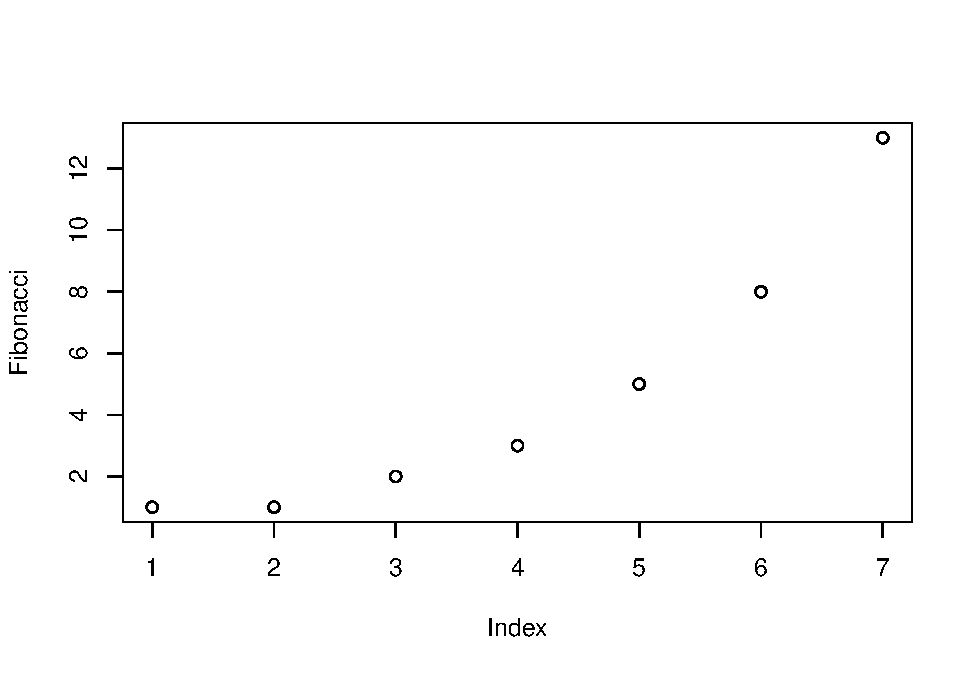
\includegraphics{navarro2_files/figure-latex/firstplot-1.pdf}
\caption{\label{fig:firstplot}Our first plot}
\end{figure}

As you can see, what R has done is plot the \emph{values} stored in the
\texttt{Fibonacci} variable on the vertical axis (y-axis) and the
corresponding \emph{index} on the horizontal axis (x-axis). In other
words, since the 4th element of the vector has a value of 3, we get a
dot plotted at the location (4,3). That's pretty straightforward, and
the image in Figure \ref{fig:firstplot} is probably pretty close to what
you would have had in mind when I suggested that we plot the
\texttt{Fibonacci} data. However, there's quite a lot of customisation
options available to you, so we should probably spend a bit of time
looking at some of those options. So, be warned: this ends up being a
fairly long section, because there's so many possibilities open to you.
Don't let it overwhelm you though\ldots{} while all of the options
discussed here are handy to know about, you can get by just fine only
knowing a few of them. The only reason I've included all this stuff
right at the beginning is that it ends up making the rest of the chapter
a lot more readable!

\subsection{A tedious digression}\label{a-tedious-digression}

Before we go into any discussion of customising plots, we need a little
more background. The important thing to note when using the
\texttt{plot()} function, is that it's another example of a
\emph{generic} function (Section \ref{generics}, much like
\texttt{print()} and \texttt{summary()}, and so its behaviour changes
depending on what kind of input you give it. However, the
\texttt{plot()} function is somewhat fancier than the other two, and its
behaviour depends on \emph{two} arguments, \texttt{x} (the first input,
which is required) and \texttt{y} (which is optional). This makes it (a)
extremely powerful once you get the hang of it, and (b) hilariously
unpredictable, when you're not sure what you're doing. As much as
possible, I'll try to make clear what type of inputs produce what kinds
of outputs. For now, however, it's enough to note that I'm only doing
very basic plotting, and as a consequence all of the work is being done
by the \texttt{plot.default()} function.

What kinds of customisations might we be interested in? If you look at
the help documentation for the default plotting method (i.e., type
\texttt{?plot.default} or \texttt{help("plot.default")}) you'll see a
very long list of arguments that you can specify to customise your plot.
I'll talk about several of them in a moment, but first I want to point
out something that might seem quite wacky. When you look at all the
different options that the help file talks about, you'll notice that
\emph{some} of the options that it refers to are ``proper'' arguments to
the \texttt{plot.default()} function, but it also goes on to mention a
bunch of things that \emph{look} like they're supposed to be arguments,
but they're not listed in the ``Usage'' section of the file, and the
documentation calls them \textbf{\emph{graphical parameters}} instead.
Even so, it's usually possible to treat them as if they were arguments
of the plotting function. Very odd. In order to stop my readers trying
to find a brick and look up my home address, I'd better explain what's
going on; or at least give the basic gist behind it.

What exactly is a graphical parameter? Basically, the idea is that there
are some characteristics of a plot which are pretty universal: for
instance, regardless of what kind of graph you're drawing, you probably
need to specify what colour to use for the plot, right? So you'd expect
there to be something like a \texttt{col} argument to every single
graphics function in R? Well, sort of. In order to avoid having hundreds
of arguments for every single function, what R does is refer to a bunch
of these ``graphical parameters'' which are pretty general purpose.
Graphical parameters can be changed directly by using the low-level
\texttt{par()} function, which I discuss briefly in Section
\ref{sec:par} though not in a lot of detail. If you look at the help
files for graphical parameters (i.e., type \texttt{?par}) you'll see
that there's \emph{lots} of them. Fortunately, (a) the default settings
are generally pretty good so you can ignore the majority of the
parameters, and (b) as you'll see as we go through this chapter, you
very rarely need to use \texttt{par()} directly, because you can
``pretend'' that graphical parameters are just additional arguments to
your high-level function (e.g. \texttt{plot.default()}). In
short\ldots{} yes, R does have these wacky ``graphical parameters''
which can be quite confusing. But in most basic uses of the plotting
functions, you can act as if they were just undocumented additional
arguments to your function.

\subsection{Customising the title and the axis labels}\label{figtitles}

One of the first things that you'll find yourself wanting to do when
customising your plot is to label it better. You might want to specify
more appropriate axis labels, add a title or add a subtitle. The
arguments that you need to specify to make this happen are:

\begin{itemize}
\tightlist
\item
  \texttt{main}. A character string containing the title.
\item
  \texttt{sub}. A character string containing the subtitle.
\item
  \texttt{xlab}. A character string containing the x-axis label.
\item
  \texttt{ylab}. A character string containing the y-axis label.
\end{itemize}

These aren't graphical parameters, they're arguments to the high-level
function. However, because the high-level functions all rely on the same
low-level function to do the drawing\footnote{The low-level function
  that does this is called \texttt{title()} in case you ever need to
  know, and you can type \texttt{?title} to find out a bit more detail
  about what these arguments do.} the names of these arguments are
identical for pretty much every high-level function I've come across.
Let's have a look at what happens when we make use of all these
arguments. Here's the command\ldots{}

\begin{verbatim}
> plot( x = Fibonacci, 
+       main = "You specify title using the 'main' argument",
+       sub = "The subtitle appears here! (Use the 'sub' argument for this)",
+       xlab = "The x-axis label is 'xlab'",
+       ylab = "The y-axis label is 'ylab'"
+ )
\end{verbatim}

The picture that this draws is shown in Figure \ref{fig:secondplot}.

\begin{figure}
\centering
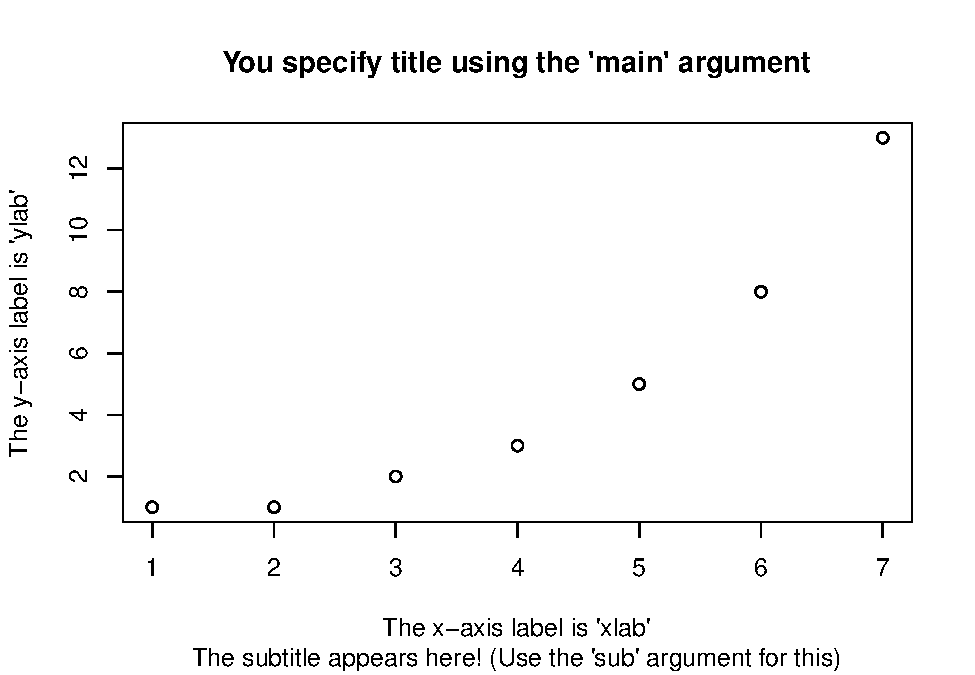
\includegraphics{navarro2_files/figure-latex/secondplot-1.pdf}
\caption{\label{fig:secondplot}How to add your own title, subtitle, x-axis
label and y-axis label to the plot.}
\end{figure}

It's more or less as you'd expect. The plot itself is identical to the
one we drew in Figure \ref{fig:firstplot}, except for the fact that
we've changed the axis labels, and added a title and a subtitle. Even
so, there's a couple of interesting features worth calling your
attention to. Firstly, notice that the subtitle is drawn below the plot,
which I personally find annoying; as a consequence I almost never use
subtitles. You may have a different opinion, of course, but the
important thing is that you remember where the subtitle actually goes.
Secondly, notice that R has decided to use boldface text and a larger
font size for the title. This is one of my most hated default settings
in R graphics, since I feel that it draws too much attention to the
title. Generally, while I do want my reader to look at the title, I find
that the R defaults are a bit overpowering, so I often like to change
the settings. To that end, there are a bunch of graphical parameters
that you can use to customise the font style:

\begin{itemize}
\tightlist
\item
  \emph{Font styles:} \texttt{font.main}, \texttt{font.sub},
  \texttt{font.lab}, \texttt{font.axis}. These four parameters control
  the font style used for the plot title (\texttt{font.main}), the
  subtitle (\texttt{font.sub}), the axis labels (\texttt{font.lab}: note
  that you can't specify separate styles for the x-axis and y-axis
  without using low level commands), and the numbers next to the tick
  marks on the axis (\texttt{font.axis}). Somewhat irritatingly, these
  arguments are numbers instead of meaningful names: a value of 1
  corresponds to plain text, 2 means boldface, 3 means italic and 4
  means bold italic.
\item
  \emph{Font colours:} \texttt{col.main}, \texttt{col.sub},
  \texttt{col.lab}, \texttt{col.axis}. These parameters do pretty much
  what the name says: each one specifies a \textbf{col}our in which to
  type each of the different bits of text. Conveniently, R has a very
  large number of named colours (type \texttt{colours()} to see a list
  of over 650 colour names that R knows), so you can use the English
  language name of the colour to select it.\footnote{On the off chance
    that this isn't enough freedom for you, you can select a colour
    directly as a ``red, green, blue'' specification using the
    \texttt{rgb()} function, or as a ``hue, saturation, value''
    specification using the \texttt{hsv()} function.} Thus, the
  parameter value here string like \texttt{"red"}, \texttt{"gray25"} or
  \texttt{"springgreen4"} (yes, R really does recognise four different
  shades of ``spring green'').
\item
  \emph{Font size:} \texttt{cex.main}, \texttt{cex.sub},
  \texttt{cex.lab}, \texttt{cex.axis}. Font size is handled in a
  slightly curious way in R. The ``cex'' part here is short for
  ``\textbf{c}haracter \textbf{ex}pansion'', and it's essentially a
  magnification value. By default, all of these are set to a value of 1,
  except for the font title: \texttt{cex.main} has a default
  magnification of 1.2, which is why the title font is 20\% bigger than
  the others.
\item
  \emph{Font family:} \texttt{family}. This argument specifies a font
  family to use: the simplest way to use it is to set it to
  \texttt{"sans"}, \texttt{"serif"}, or \texttt{"mono"}, corresponding
  to a san serif font, a serif font, or a monospaced font. If you want
  to, you can give the name of a specific font, but keep in mind that
  different operating systems use different fonts, so it's probably
  safest to keep it simple. Better yet, unless you have some deep
  objections to the R defaults, just ignore this parameter entirely.
  That's what I usually do.
\end{itemize}

To give you a sense of how you can use these parameters to customise
your titles, the following command can be used to draw Figure
\ref{fig:thirdplot}:

\begin{verbatim}
> plot( x = Fibonacci,                           # the data to plot
+       main = "The first 7 Fibonacci numbers",  # the title 
+       xlab = "Position in the sequence",       # x-axis label
+       ylab = "The Fibonacci number",           # y-axis label
+       font.main = 1,                           # plain text for title 
+       cex.main = 1,                            # normal size for title
+       font.axis = 2,                           # bold text for numbering
+       col.lab = "gray50"                       # grey colour for labels
+ )
\end{verbatim}

\begin{figure}
\centering
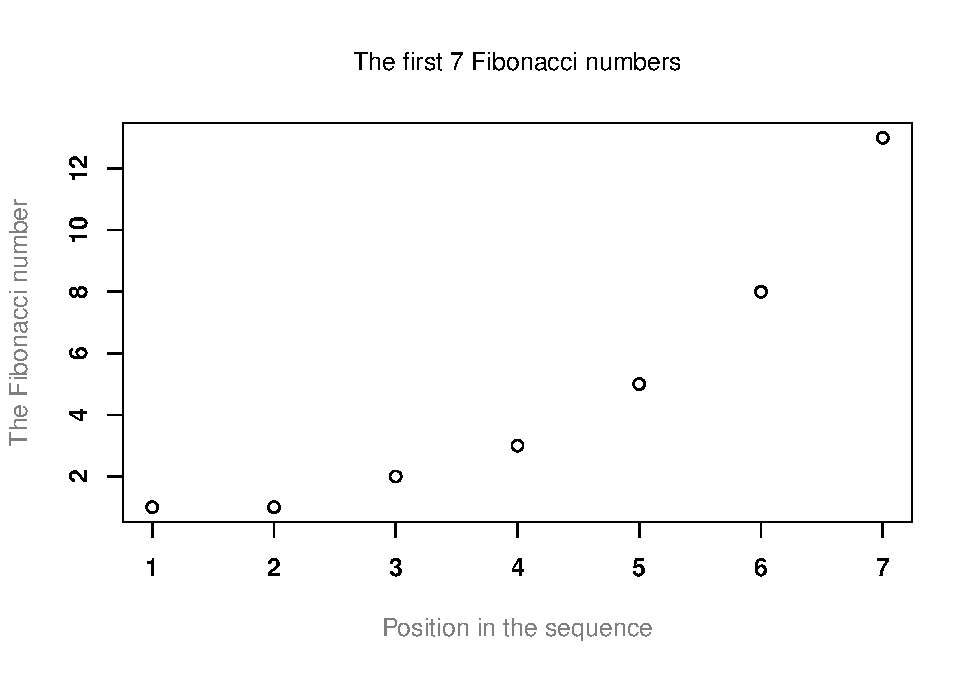
\includegraphics{navarro2_files/figure-latex/thirdplot-1.pdf}
\caption{\label{fig:thirdplot}How to customise the appearance of the titles
and labels.}
\end{figure}

Although this command is quite long, it's not complicated: all it does
is override a bunch of the default parameter values. The only difficult
aspect to this is that you have to remember what each of these
parameters is called, and what all the different values are. And in
practice I never remember: I have to look up the help documentation
every time, or else look it up in this book.

\subsection{Changing the plot type}\label{changing-the-plot-type}

Adding and customising the titles associated with the plot is one way in
which you can play around with what your picture looks like. Another
thing that you'll want to do is customise the appearance of the actual
plot! To start with, let's look at the single most important options
that the \texttt{plot()} function (or, recalling that we're dealing with
a generic function, in this case the \texttt{plot.default()} function,
since that's the one doing all the work) provides for you to use, which
is the \texttt{type} argument. The type argument specifies the visual
style of the plot. The possible values for this are:

\begin{itemize}
\tightlist
\item
  \texttt{type\ =\ "p"}. Draw the \textbf{p}oints only.
\item
  \texttt{type\ =\ "l"}. Draw a \textbf{l}ine through the points.
\item
  \texttt{type\ =\ "o"}. Draw the line \textbf{o}ver the top of the
  points.
\item
  \texttt{type\ =\ "b"}. Draw \textbf{b}oth points and lines, but don't
  overplot.
\item
  \texttt{type\ =\ "h"}. Draw ``\textbf{h}istogram-like'' vertical bars.
\item
  \texttt{type\ =\ "s"}. Draw a \textbf{s}taircase, going horizontally
  then vertically.
\item
  \texttt{type\ =\ "S"}. Draw a \textbf{S}taircase, going vertically
  then horizontally.
\item
  \texttt{type\ =\ "c"}. Draw only the \textbf{c}onnecting lines from
  the ``b'' version.
\item
  \texttt{type\ =\ "n"}. Draw nothing. (Apparently this is useful
  sometimes?)
\end{itemize}

The simplest way to illustrate what each of these really looks like is
just to draw them. To that end, Figure \ref{fig:simpleplots} shows the
same Fibonacci data, drawn using six different \texttt{types} of plot.
As you can see, by altering the type argument you can get a
qualitatively different appearance to your plot. In other words, as far
as R is concerned, the only difference between a scatterplot (like the
ones we drew in Section \ref{correl} and a line plot is that you draw a
scatterplot by setting \texttt{type\ =\ "p"} and you draw a line plot by
setting \texttt{type\ =\ "l"}. However, that doesn't imply that
\emph{you} should think of them as begin equivalent to each other. As
you can see by looking at Figure \ref{fig:simpleplots}, a line plot
implies that there is some notion of continuity from one point to the
next, whereas a scatterplot does not.

\begin{figure}
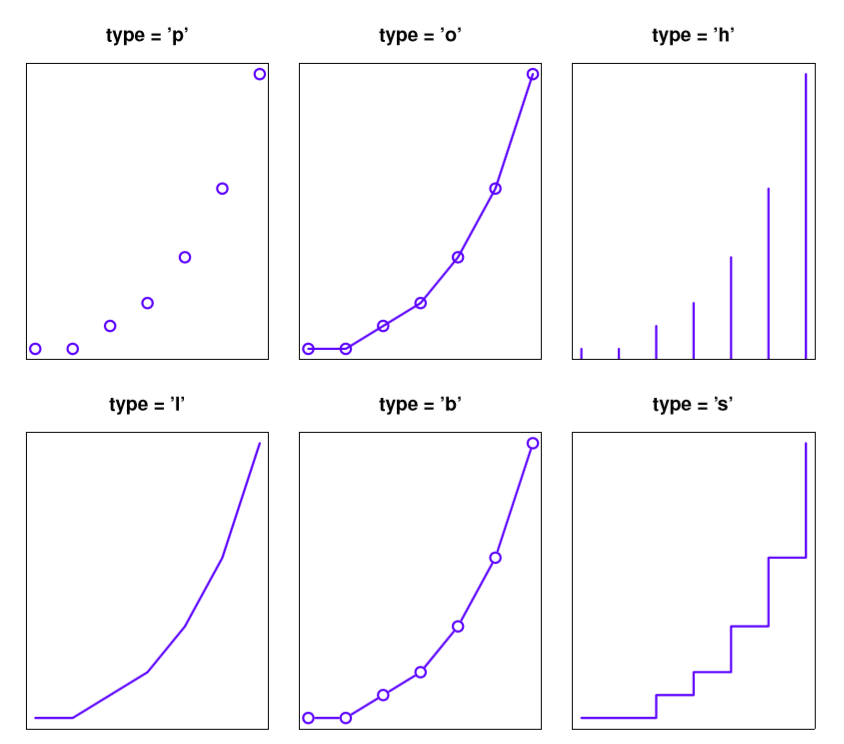
\includegraphics[width=11.72in]{./rbook-master/img/graphics2/simpleplot} \caption{Changing the `type` of the plot.}\label{fig:simpleplots}
\end{figure}

\subsection{Changing other features of the
plot}\label{changing-other-features-of-the-plot}

\begin{figure}
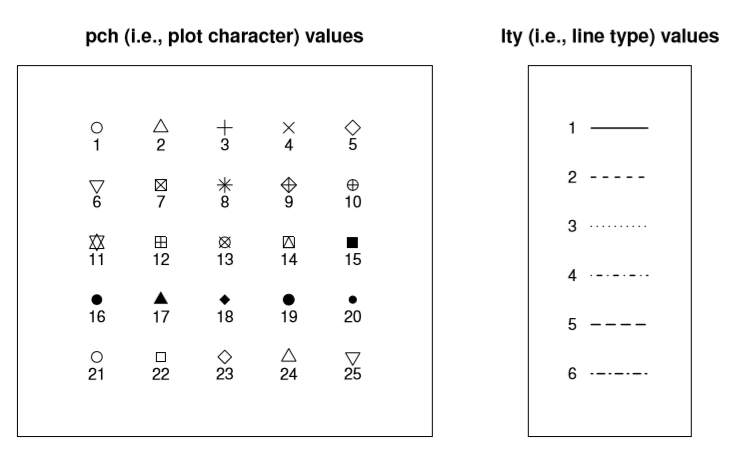
\includegraphics[width=10.22in]{./rbook-master/img/graphics2/pchlty} \caption{Changing the line and plotted characters of the plot.}\label{fig:pch}
\end{figure}

In Section \ref{sec:figtitles} we talked about a group of graphical
parameters that are related to the formatting of titles, axis labels
etc. The second group of parameters I want to discuss are those related
to the formatting of the plot itself:

\begin{itemize}
\tightlist
\item
  \emph{Colour of the plot}: \texttt{col}. As we saw with the previous
  colour-related parameters, the simplest way to specify this parameter
  is using a character string: e.g., \texttt{col\ =\ "blue"}. It's a
  pretty straightforward parameter to specify: the only real subtlety is
  that every high-level function tends to draw a different ``thing'' as
  it's output, and so this parameter gets interpreted a little
  differently by different functions. However, for the
  \texttt{plot.default()} function it's pretty simple: the \texttt{col}
  argument refers to the colour of the points and/or lines that get
  drawn!
\item
  \emph{Character used to plot points}: \texttt{pch}. The \textbf{p}lot
  \textbf{ch}aracter parameter is a number, usually between 1 and 25.
  What it does is tell R what symbol to use to draw the points that it
  plots. The simplest way to illustrate what the different values do is
  with a picture. Figure \ref{fig:pch}a shows the first 25 plotting
  characters. The default plotting character is a hollow circle (i.e.,
  \texttt{pch\ =\ 1}).
\item
  \emph{Plot size}: \texttt{cex}. This parameter describes a
  \textbf{c}haracter \textbf{ex}pansion factor (i.e., magnification) for
  the plotted characters. By default \texttt{cex=1}, but if you want
  bigger symbols in your graph you should specify a larger value.
\item
  \emph{Line type}: \texttt{lty}. The \textbf{l}ine \textbf{ty}pe
  parameter describes the kind of line that R draws. It has seven values
  which you can specify using a number between \texttt{0} and
  \texttt{7}, or using a meaningful character string: \texttt{"blank"},
  \texttt{"solid"}, \texttt{"dashed"}, \texttt{"dotted"},
  \texttt{"dotdash"}, \texttt{"longdash"}, or \texttt{"twodash"}. Note
  that the ``blank'' version (value 0) just means that R doesn't draw
  the lines at all. The other six versions are shown in Figure
  \ref{fig:pch}b.
\item
  \emph{Line width}: \texttt{lwd}. The last graphical parameter in this
  category that I want to mention is the \textbf{l}ine
  \textbf{w}i\textbf{d}th parameter, which is just a number specifying
  the width of the line. The default value is 1. Not surprisingly,
  larger values produce thicker lines and smaller values produce thinner
  lines. Try playing around with different values of \texttt{lwd} to see
  what happens.
\end{itemize}

To illustrate what you can do by altering these parameters, let's try
the following command:

\begin{verbatim}
> plot( x = Fibonacci,   # the data set
+       type = "b",      # plot both points and lines
+       col = "blue",    # change the plot colour to blue
+       pch = 19,        # plotting character is a solid circle
+       cex = 5,         # plot it at 5x the usual size
+       lty = 2,         # change line type to dashed
+       lwd = 4          # change line width to 4x the usual
+ )
\end{verbatim}

The output is shown in Figure \ref{fig:fifthplot}.

\begin{Shaded}
\begin{Highlighting}[]
\KeywordTok{plot}\NormalTok{( }\DataTypeTok{x =}\NormalTok{ Fibonacci,}
         \DataTypeTok{type =} \StringTok{"b"}\NormalTok{,}
         \DataTypeTok{col =} \StringTok{"blue"}\NormalTok{,}
         \DataTypeTok{pch =} \DecValTok{19}\NormalTok{,}
         \DataTypeTok{cex=}\DecValTok{5}\NormalTok{,}
         \DataTypeTok{lty=}\DecValTok{2}\NormalTok{,}
         \DataTypeTok{lwd=}\DecValTok{4}\NormalTok{)}
\end{Highlighting}
\end{Shaded}

\begin{figure}
\centering
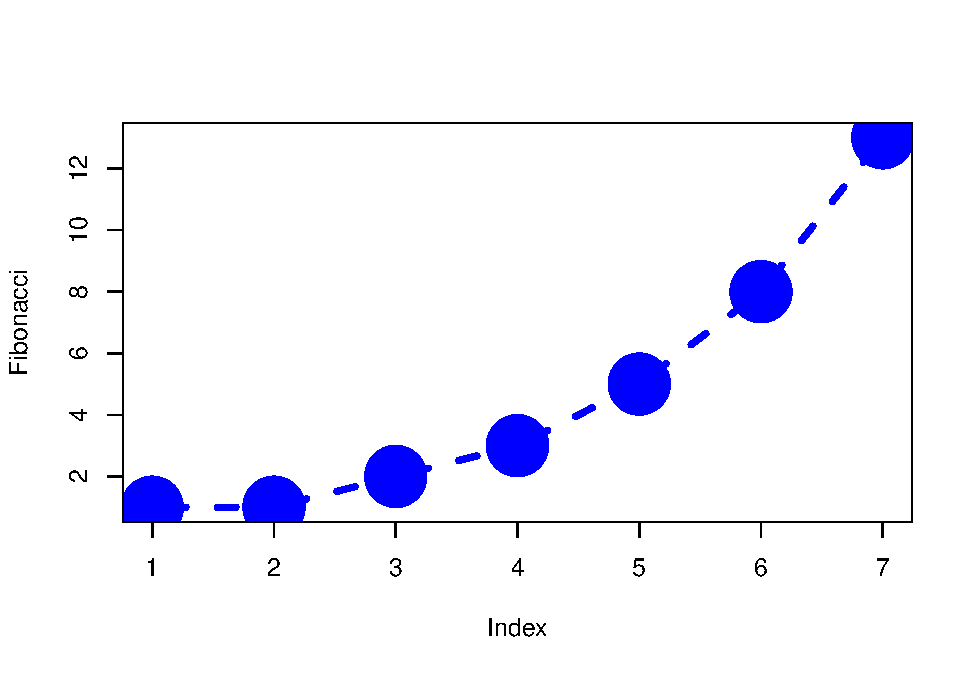
\includegraphics{navarro2_files/figure-latex/fifthplot-1.pdf}
\caption{\label{fig:fifthplot}Customising various aspects to the plot
itself.}
\end{figure}

\subsection{Changing the appearance of the
axes}\label{changing-the-appearance-of-the-axes}

There are several other possibilities worth discussing. Ignoring
graphical parameters for the moment, there's a few other arguments to
the \texttt{plot.default()} function that you might want to use. As
before, many of these are standard arguments that are used by a lot of
high level graphics functions:

\begin{itemize}
\tightlist
\item
  \emph{Changing the axis scales}: \texttt{xlim}, \texttt{ylim}.
  Generally R does a pretty good job of figuring out where to set the
  edges of the plot. However, you can override its choices by setting
  the \texttt{xlim} and \texttt{ylim} arguments. For instance, if I
  decide I want the vertical scale of the plot to run from 0 to 100,
  then I'd set \texttt{ylim\ =\ c(0,\ 100)}.
\item
  \emph{Suppress labelling}: \texttt{ann}. This is a logical-valued
  argument that you can use if you don't want R to include any text for
  a title, subtitle or axis label. To do so, set \texttt{ann\ =\ FALSE}.
  This will stop R from including any text that would normally appear in
  those places. Note that this will override any of your manual titles.
  For example, if you try to add a title using the \texttt{main}
  argument, but you also specify \texttt{ann\ =\ FALSE}, no title will
  appear.
\item
  \emph{Suppress axis drawing}: \texttt{axes}. Again, this is a logical
  valued argument. Suppose you don't want R to draw any axes at all. To
  suppress the axes, all you have to do is add \texttt{axes\ =\ FALSE}.
  This will remove the axes and the numbering, but not the axis labels
  (i.e.~the \texttt{xlab} and \texttt{ylab} text). Note that you can get
  finer grain control over this by specifying the \texttt{xaxt} and
  \texttt{yaxt} graphical parameters instead (see below).
\item
  \emph{Include a framing box}: \texttt{frame.plot}. Suppose you've
  removed the axes by setting \texttt{axes\ =\ FALSE}, but you still
  want to have a simple box drawn around the plot; that is, you only
  wanted to get rid of the numbering and the tick marks, but you want to
  keep the box. To do that, you set \texttt{frame.plot\ =\ TRUE}.
\end{itemize}

Note that this list isn't exhaustive. There are a few other arguments to
the \texttt{plot.default} function that you can play with if you want
to, but those are the ones you are probably most likely to want to use.
As always, however, if these aren't enough options for you, there's also
a number of other graphical parameters that you might want to play with
as well. That's the focus of the next section. In the meantime, here's a
command that makes use of all these different options:

\begin{verbatim}
> plot( x = Fibonacci,       # the data
+       xlim = c(0, 15),     # expand the x-scale
+       ylim = c(0, 15),     # expand the y-scale
+       ann = FALSE,         # delete all annotations
+       axes = FALSE,        # delete the axes
+       frame.plot = TRUE    # but include a framing box
+ )
\end{verbatim}

The output is shown in Figure \ref{fig:fourthplot}, and it's pretty much
exactly as you'd expect. The axis scales on both the horizontal and
vertical dimensions have been expanded, the axes have been suppressed as
have the annotations, but I've kept a box around the plot.

\begin{Shaded}
\begin{Highlighting}[]
    \KeywordTok{plot}\NormalTok{( }\DataTypeTok{x =}\NormalTok{ Fibonacci,}
          \DataTypeTok{xlim =} \KeywordTok{c}\NormalTok{(}\DecValTok{0}\NormalTok{, }\DecValTok{15}\NormalTok{),}
          \DataTypeTok{ylim =} \KeywordTok{c}\NormalTok{(}\DecValTok{0}\NormalTok{, }\DecValTok{15}\NormalTok{),}
              \DataTypeTok{ann =} \OtherTok{FALSE}\NormalTok{,}
          \DataTypeTok{axes =} \OtherTok{FALSE}\NormalTok{,}
            \DataTypeTok{frame.plot =} \OtherTok{TRUE}\NormalTok{)}
\end{Highlighting}
\end{Shaded}

\begin{figure}
\centering
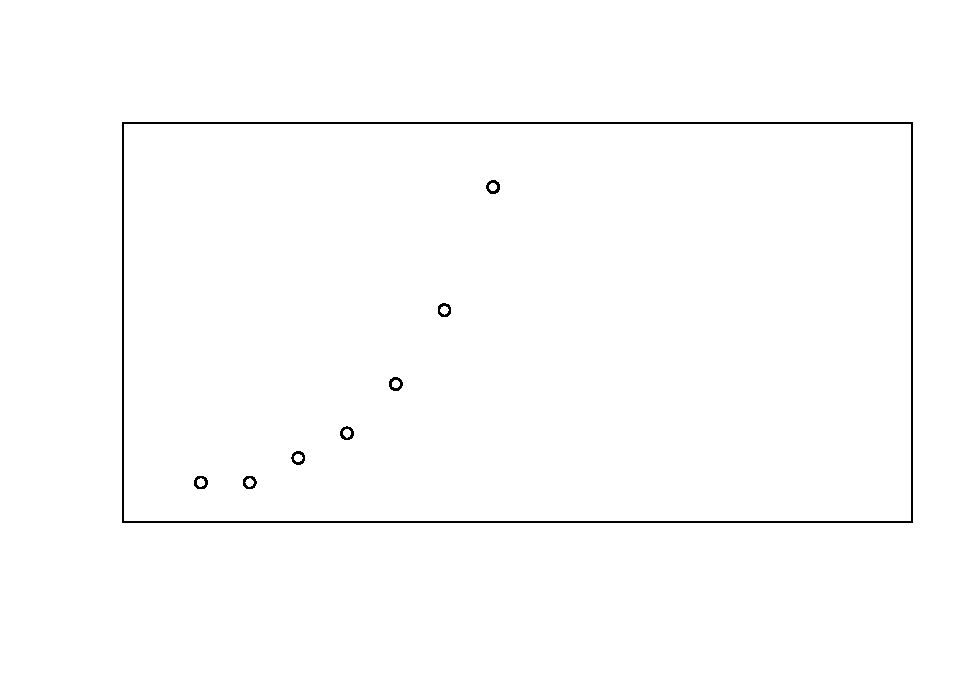
\includegraphics{navarro2_files/figure-latex/fourthplot-1.pdf}
\caption{\label{fig:fourthplot}Altering the scale and appearance of the plot
axes.}
\end{figure}

Before moving on, I should point out that there are several graphical
parameters relating to the axes, the box, and the general appearance of
the plot which allow finer grain control over the appearance of the axes
and the annotations.

\begin{itemize}
\tightlist
\item
  \emph{Suppressing the axes individually}: \texttt{xaxt},
  \texttt{yaxt}. These graphical parameters are basically just fancier
  versions of the \texttt{axes} argument we discussed earlier. If you
  want to stop R from drawing the vertical axis but you'd like it to
  keep the horizontal axis, set \texttt{yaxt\ =\ "n"}. I trust that you
  can figure out how to keep the vertical axis and suppress the
  horizontal one!
\item
  \emph{Box type}: \texttt{bty}. In the same way that \texttt{xaxt},
  \texttt{yaxt} are just fancy versions of \texttt{axes}, the
  \textbf{b}ox \textbf{ty}pe parameter is really just a fancier version
  of the \texttt{frame.plot} argument, allowing you to specify exactly
  which out of the four borders you want to keep. The way we specify
  this parameter is a bit stupid, in my opinion: the possible values are
  \texttt{"o"} (the default), \texttt{"l"}, \texttt{"7"}, \texttt{"c"},
  \texttt{"u"}, or \texttt{"{]}"}, each of which will draw only those
  edges that the corresponding character suggests. That is, the letter
  \texttt{"c"} has a top, a bottom and a left, but is blank on the right
  hand side, whereas \texttt{"7"} has a top and a right, but is blank on
  the left and the bottom. Alternatively a value of \texttt{"n"} means
  that no box will be drawn.
\item
  \emph{Orientation of the axis labels} \texttt{las}. I presume that the
  name of this parameter is an acronym of \textbf{la}bel \textbf{s}tyle
  or something along those lines; but what it actually does is govern
  the orientation of the text used to label the individual tick marks
  (i.e., the numbering, not the \texttt{xlab} and \texttt{ylab} axis
  labels). There are four possible values for \texttt{las}: A value of 0
  means that the labels of both axes are printed parallel to the axis
  itself (the default). A value of 1 means that the text is always
  horizontal. A value of 2 means that the labelling text is printed at
  right angles to the axis. Finally, a value of 3 means that the text is
  always vertical.
\end{itemize}

Again, these aren't the only possibilities. There are a few other
graphical parameters that I haven't mentioned that you could use to
customise the appearance of the axes,\footnote{Also, there's a low level
  function called \texttt{axis()} that allows a lot more control over
  the appearance of the axes.} but that's probably enough (or more than
enough) for now. To give a sense of how you could use these parameters,
let's try the following command:

\begin{verbatim}
> plot( x = Fibonacci,   # the data
+       xaxt = "n",      # don't draw the x-axis
+       bty = "]",       # keep bottom, right and top of box only
+       las = 1          # rotate the text
+ )
\end{verbatim}

The output is shown in Figure \ref{fig:sixthplot}. As you can see, this
isn't a very useful plot at all. However, it does illustrate the
graphical parameters we're talking about, so I suppose it serves its
purpose.

\begin{Shaded}
\begin{Highlighting}[]
    \KeywordTok{plot}\NormalTok{( }\DataTypeTok{x =}\NormalTok{ Fibonacci,}
         \DataTypeTok{xaxt =} \StringTok{"n"}\NormalTok{,}
         \DataTypeTok{bty =} \StringTok{"]"}\NormalTok{,}
         \DataTypeTok{las =} \DecValTok{1}\NormalTok{ )}
\end{Highlighting}
\end{Shaded}

\begin{figure}
\centering
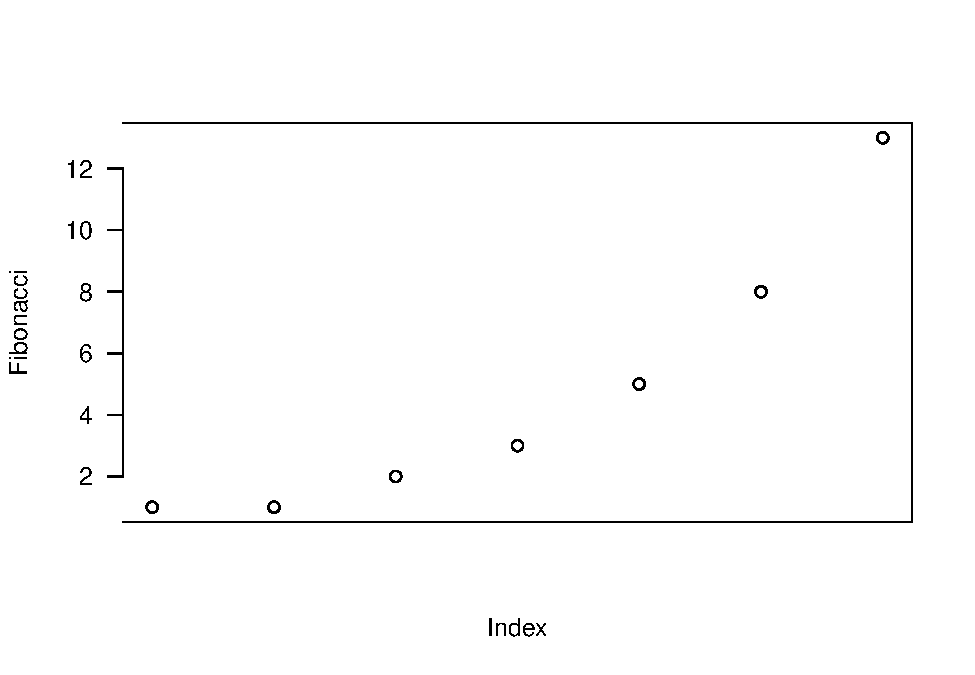
\includegraphics{navarro2_files/figure-latex/sixthplot-1.pdf}
\caption{\label{fig:sixthplot}Other ways to customise the axes}
\end{figure}

\subsection{Don't panic}\label{dont-panic}

At this point, a lot of readers will be probably be thinking something
along the lines of, ``if there's this much detail just for drawing a
simple plot, how horrible is it going to get when we start looking at
more complicated things?'' Perhaps, contrary to my earlier pleas for
mercy, you've found a brick to hurl and are right now leafing through an
Adelaide phone book trying to find my address. Well, fear not! And
please, put the brick down. In a lot of ways, we've gone through the
hardest part: we've already covered vast majority of the plot
customisations that you might want to do. As you'll see, each of the
other high level plotting commands we'll talk about will only have a
smallish number of additional options. Better yet, even though I've told
you about a billion different ways of tweaking your plot, you don't
usually need them. So in practice, now that you've read over it once to
get the gist, the majority of the content of this section is stuff you
can safely forget: just remember to come back to this section later on
when you want to tweak your plot.

\section{Histograms}\label{hist}

Now that we've tamed (or possibly fled from) the beast that is R
graphical parameters, let's talk more seriously about some real life
graphics that you'll want to draw. We begin with the humble
\textbf{\emph{histogram}}. Histograms are one of the simplest and most
useful ways of visualising data. They make most sense when you have an
interval or ratio scale (e.g., the \texttt{afl.margins} data from
Chapter \ref{descriptives} and what you want to do is get an overall
impression of the data. Most of you probably know how histograms work,
since they're so widely used, but for the sake of completeness I'll
describe them. All you do is divide up the possible values into
\textbf{\emph{bins}}, and then count the number of observations that
fall within each bin. This count is referred to as the frequency of the
bin, and is displayed as a bar: in the AFL winning margins data, there
are 33 games in which the winning margin was less than 10 points, and it
is this fact that is represented by the height of the leftmost bar in
Figure \ref{fig:hist1a}. Drawing this histogram in R is pretty
straightforward. The function you need to use is called \texttt{hist()},
and it has pretty reasonable default settings. In fact, Figure
\ref{fig:hist1a} is exactly what you get if you just type this:

\begin{verbatim}
> hist( afl.margins )   # panel a
\end{verbatim}

\begin{Shaded}
\begin{Highlighting}[]
\KeywordTok{load}\NormalTok{(}\StringTok{"./rbook-master/data/aflsmall.Rdata"}\NormalTok{)}
\KeywordTok{hist}\NormalTok{(afl.margins)   }\CommentTok{# panel a}
\end{Highlighting}
\end{Shaded}

\begin{figure}
\centering
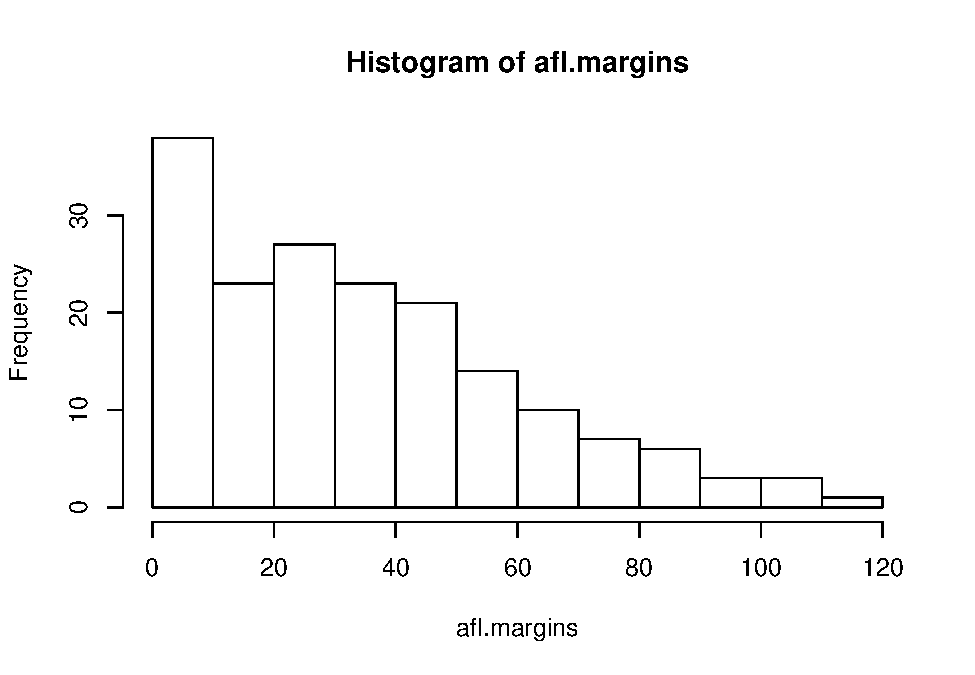
\includegraphics{navarro2_files/figure-latex/hist1a-1.pdf}
\caption{\label{fig:hist1a}The default histogram that R produces}
\end{figure}

Although this image would need a lot of cleaning up in order to make a
good presentation graphic (i.e., one you'd include in a report), it
nevertheless does a pretty good job of describing the data. In fact, the
big strength of a histogram is that (properly used) it does show the
entire spread of the data, so you can get a pretty good sense about what
it looks like. The downside to histograms is that they aren't very
compact: unlike some of the other plots I'll talk about it's hard to
cram 20-30 histograms into a single image without overwhelming the
viewer. And of course, if your data are nominal scale (e.g., the
\texttt{afl.finalists} data) then histograms are useless.

The main subtlety that you need to be aware of when drawing histograms
is determining where the \texttt{breaks} that separate bins should be
located, and (relatedly) how many breaks there should be. In Figure
\ref{fig:hist1a}, you can see that R has made pretty sensible choices
all by itself: the breaks are located at 0, 10, 20, \ldots{} 120, which
is exactly what I would have done had I been forced to make a choice
myself. On the other hand, consider the two histograms in Figure
\ref{fig:hist1b} and \ref{fig:hist1c}, which I produced using the
following two commands:

\begin{Shaded}
\begin{Highlighting}[]
\KeywordTok{hist}\NormalTok{( }\DataTypeTok{x =}\NormalTok{ afl.margins, }\DataTypeTok{breaks =} \DecValTok{3}\NormalTok{ )      }\CommentTok{# panel b}
\end{Highlighting}
\end{Shaded}

\begin{figure}
\centering
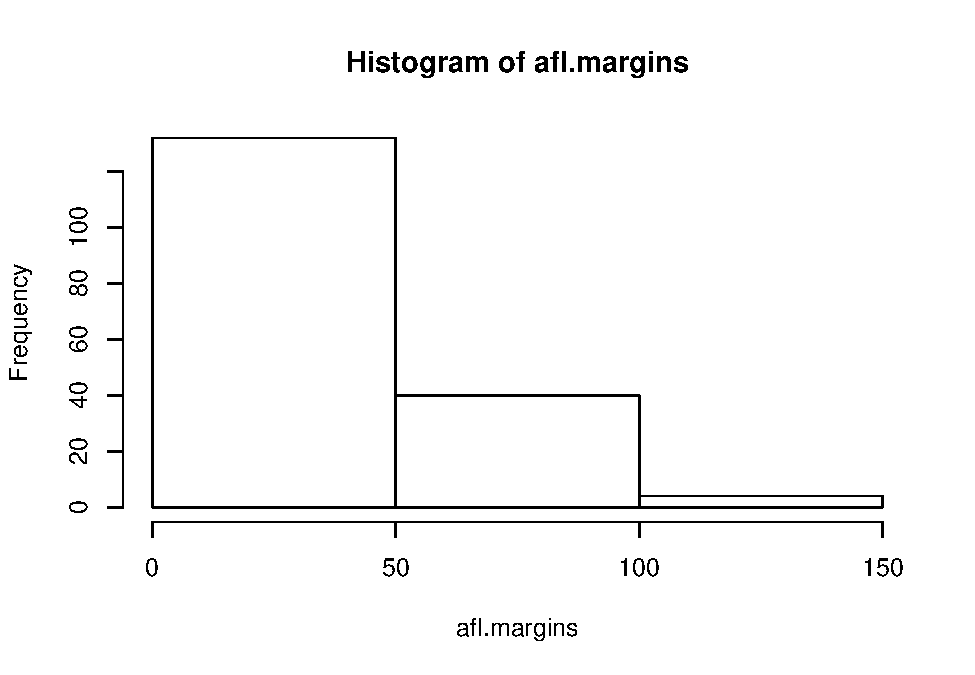
\includegraphics{navarro2_files/figure-latex/hist1b-1.pdf}
\caption{\label{fig:hist1b}A histogram with too few bins}
\end{figure}

\begin{Shaded}
\begin{Highlighting}[]
\KeywordTok{hist}\NormalTok{( }\DataTypeTok{x =}\NormalTok{ afl.margins, }\DataTypeTok{breaks =} \DecValTok{0}\OperatorTok{:}\DecValTok{116}\NormalTok{ )  }\CommentTok{# panel c}
\end{Highlighting}
\end{Shaded}

\begin{figure}
\centering
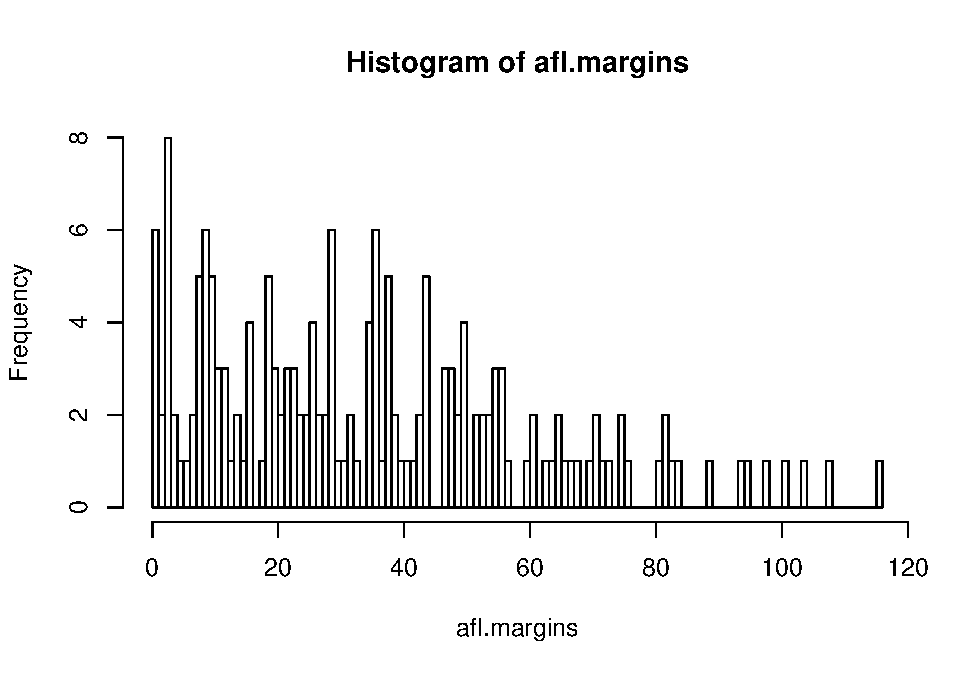
\includegraphics{navarro2_files/figure-latex/hist1c-1.pdf}
\caption{\label{fig:hist1c}A histogram with too many bins}
\end{figure}

In Figure \ref{fig:hist1c}, the bins are only 1 point wide. As a result,
although the plot is very informative (it displays the entire data set
with no loss of information at all!) the plot is very hard to interpret,
and feels quite cluttered. On the other hand, the plot in Figure
\ref{fig:hist1b} has a bin width of 50 points, and has the opposite
problem: it's very easy to ``read'' this plot, but it doesn't convey a
lot of information. One gets the sense that this histogram is hiding too
much. In short, the way in which you specify the breaks has a big effect
on what the histogram looks like, so it's important to make sure you
choose the breaks sensibly. In general R does a pretty good job of
selecting the breaks on its own, since it makes use of some quite clever
tricks that statisticians have devised for automatically selecting the
right bins for a histogram, but nevertheless it's usually a good idea to
play around with the breaks a bit to see what happens.

There is one fairly important thing to add regarding how the
\texttt{breaks} argument works. There are two different ways you can
specify the breaks. You can either specify \emph{how many} breaks you
want (which is what I did for panel b when I typed
\texttt{breaks\ =\ 3}) and let R figure out where they should go, or you
can provide a vector that tells R exactly where the breaks should be
placed (which is what I did for panel c when I typed
\texttt{breaks\ =\ 0:116}). The behaviour of the \texttt{hist()}
function is slightly different depending on which version you use. If
all you do is tell it \emph{how many} breaks you want, R treats it as a
``suggestion'' not as a demand. It assumes you want ``approximately 3''
breaks, but if it doesn't think that this would look very pretty on
screen, it picks a different (but similar) number. It does this for a
sensible reason -- it tries to make sure that the breaks are located at
sensible values (like 10) rather than stupid ones (like 7.224414). And
most of the time R is right: usually, when a human researcher says
``give me 3 breaks'', he or she really does mean ``give me approximately
3 breaks, and don't put them in stupid places''. However, sometimes R is
dead wrong. Sometimes you really do mean ``exactly 3 breaks'', and you
know precisely where you want them to go. So you need to invoke ``real
person privilege'', and order R to do what it's bloody well told. In
order to do that, you \emph{have} to input the full vector that tells R
exactly where you want the breaks. If you do that, R will go back to
behaving like the nice little obedient calculator that it's supposed to
be.

\subsection{Visual style of your
histogram}\label{visual-style-of-your-histogram}

Okay, so at this point we can draw a basic histogram, and we can alter
the number and even the location of the \texttt{breaks}. However, the
visual style of the histograms shown in Figure @ref(fig:hist1a; hist1b;
hist1c) could stand to be improved. We can fix this by making use of
some of the other arguments to the \texttt{hist()} function. Most of the
things you might want to try doing have already been covered in Section
\ref{introplotting}, but there's a few new things:

\begin{itemize}
\tightlist
\item
  \emph{Shading lines}: \texttt{density}, \texttt{angle}. You can add
  diagonal lines to shade the bars: the \texttt{density} value is a
  number indicating how many lines per inch R should draw (the default
  value of \texttt{NULL} means no lines), and the \texttt{angle} is a
  number indicating how many degrees from horizontal the lines should be
  drawn at (default is \texttt{angle\ =\ 45} degrees).
\item
  \emph{Specifics regarding colours}: \texttt{col}, \texttt{border}. You
  can also change the colours: in this instance the \texttt{col}
  parameter sets the colour of the shading (either the shading lines if
  there are any, or else the colour of the interior of the bars if there
  are not), and the \texttt{border} argument sets the colour of the
  edges of the bars.
\item
  \emph{Labelling the bars}: \texttt{labels}. You can also attach labels
  to each of the bars using the \texttt{labels} argument. The simplest
  way to do this is to set \texttt{labels\ =\ TRUE}, in which case R
  will add a number just above each bar, that number being the exact
  number of observations in the bin. Alternatively, you can choose the
  labels yourself, by inputting a vector of strings, e.g.,
  \texttt{labels\ =\ c("label\ 1","label\ 2","etc")}
\end{itemize}

Not surprisingly, this doesn't exhaust the possibilities. If you type
\texttt{help("hist")} or \texttt{?hist} and have a look at the help
documentation for histograms, you'll see a few more options. A histogram
that makes use of the histogram-specific customisations as well as
several of the options we discussed in Section \ref{sec:introplotting}
is shown in Figure \ref{fig:hist1d}. The R command that I used to draw
it is this:

\begin{Shaded}
\begin{Highlighting}[]
\KeywordTok{hist}\NormalTok{( }\DataTypeTok{x =}\NormalTok{ afl.margins, }
      \DataTypeTok{main =} \StringTok{"2010 AFL margins"}\NormalTok{, }\CommentTok{# title of the plot}
      \DataTypeTok{xlab =} \StringTok{"Margin"}\NormalTok{,           }\CommentTok{# set the x-axis label}
      \DataTypeTok{density =} \DecValTok{10}\NormalTok{,              }\CommentTok{# draw shading lines: 10 per inch}
      \DataTypeTok{angle =} \DecValTok{40}\NormalTok{,                }\CommentTok{# set the angle of the shading lines is 40 degrees}
      \DataTypeTok{border =} \StringTok{"gray20"}\NormalTok{,         }\CommentTok{# set the colour of the borders of the bars}
      \DataTypeTok{col =} \StringTok{"gray80"}\NormalTok{,            }\CommentTok{# set the colour of the shading lines}
      \DataTypeTok{labels =} \OtherTok{TRUE}\NormalTok{,             }\CommentTok{# add frequency labels to each bar}
      \DataTypeTok{ylim =} \KeywordTok{c}\NormalTok{(}\DecValTok{0}\NormalTok{,}\DecValTok{40}\NormalTok{)             }\CommentTok{# change the scale of the y-axis}
\NormalTok{)}
\end{Highlighting}
\end{Shaded}

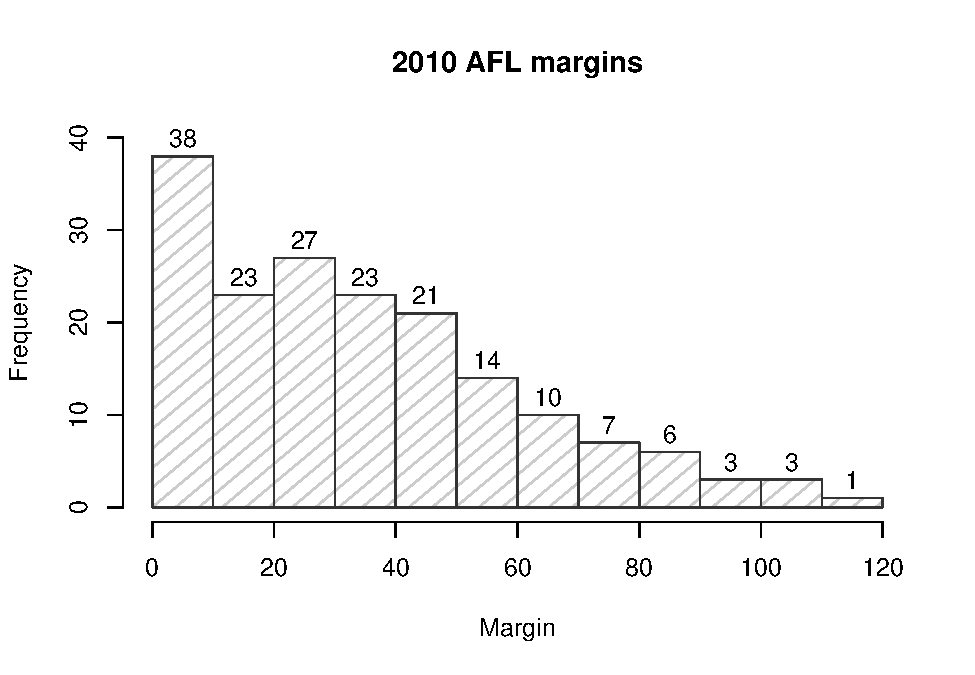
\includegraphics{navarro2_files/figure-latex/hist1d-1.pdf}

Overall, this is a much nicer histogram than the default ones.

\section{Stem and leaf plots}\label{stem}

Histograms are one of the most widely used methods for displaying the
observed values for a variable. They're simple, pretty, and very
informative. However, they do take a little bit of effort to draw.
Sometimes it can be quite useful to make use of simpler, if less
visually appealing, options. One such alternative is the
\textbf{\emph{stem and leaf plot}}. To a first approximation you can
think of a stem and leaf plot as a kind of text-based histogram. Stem
and leaf plots aren't used as widely these days as they were 30 years
ago, since it's now just as easy to draw a histogram as it is to draw a
stem and leaf plot. Not only that, they don't work very well for larger
data sets. As a consequence you probably won't have as much of a need to
use them yourself, though you may run into them in older publications.
These days, the only real world situation where I use them is if I have
a small data set with 20-30 data points and I don't have a computer
handy, because it's pretty easy to quickly sketch a stem and leaf plot
by hand.

With all that as background, lets have a look at stem and leaf plots.
The AFL margins data contains 176 observations, which is at the upper
end for what you can realistically plot this way. The function in R for
drawing stem and leaf plots is called \texttt{stem()} and if we ask for
a stem and leaf plot of the \texttt{afl.margins} data, here's what we
get:

\begin{Shaded}
\begin{Highlighting}[]
\KeywordTok{stem}\NormalTok{( afl.margins )}
\end{Highlighting}
\end{Shaded}

\begin{verbatim}
## 
##   The decimal point is 1 digit(s) to the right of the |
## 
##    0 | 001111223333333344567788888999999
##    1 | 0000011122234456666899999
##    2 | 00011222333445566667788999999
##    3 | 01223555566666678888899
##    4 | 012334444477788899
##    5 | 00002233445556667
##    6 | 0113455678
##    7 | 01123556
##    8 | 122349
##    9 | 458
##   10 | 148
##   11 | 6
\end{verbatim}

The values to the left of the \texttt{\textbar{}} are called
\textbf{\emph{stems}} and the values to the right are called
\textbf{\emph{leaves}}. If you just look at the shape that the leaves
make, you can see something that looks a lot like a histogram made out
of numbers, just rotated by 90 degrees. But if you know how to read the
plot, there's quite a lot of additional information here. In fact, it's
also giving you the actual values of \emph{all} of the observations in
the data set. To illustrate, let's have a look at the last line in the
stem and leaf plot, namely \texttt{11\ \textbar{}\ 6}. Specifically,
let's compare this to the largest values of the \texttt{afl.margins}
data set:

\begin{verbatim}
> max( afl.margins )
[1] 116
\end{verbatim}

Hm\ldots{} \texttt{11\ \textbar{}\ 6} versus \texttt{116}. Obviously the
stem and leaf plot is trying to tell us that the largest value in the
data set is 116. Similarly, when we look at the line that reads
\texttt{10\ \textbar{}\ 148}, the way we interpret it to note that the
stem and leaf plot is telling us that the data set contains observations
with values 101, 104 and 108. Finally, when we see something like
\texttt{5\ \textbar{}\ 00002233445556667} the four \texttt{0}s in the
the stem and leaf plot are telling us that there are four observations
with value 50.

I won't talk about them in a lot of detail, but I should point out that
some customisation options are available for stem and leaf plots in R.
The two arguments that you can use to do this are:

\begin{itemize}
\tightlist
\item
  \texttt{scale}. Changing the \texttt{scale} of the plot (default value
  is 1), which is analogous to changing the number of breaks in a
  histogram. Reducing the scale causes R to reduce the number of stem
  values (i.e., the number of breaks, if this were a histogram) that the
  plot uses.
\item
  \texttt{width}. The second way that to can customise a stem and leaf
  plot is to alter the \texttt{width} (default value is 80). Changing
  the width alters the maximum number of leaf values that can be
  displayed for any given stem.
\end{itemize}

However, since stem and leaf plots aren't as important as they used to
be, I'll leave it to the interested reader to investigate these options.
Try the following two commands to see what happens:

\begin{verbatim}
> stem( x = afl.margins, scale = .25 )
> stem( x = afl.margins, width = 20 )
\end{verbatim}

The only other thing to note about stem and leaf plots is the line in
which R tells you where the decimal point is. If our data set had
included only the numbers .11, .15, .23, .35 and .59 and we'd drawn a
stem and leaf plot of these data, then R would move the decimal point:
the stem values would be 1,2,3,4 and 5, but R would tell you that the
decimal point has moved to the left of the \texttt{\textbar{}} symbol.
If you want to see this in action, try the following command:

\begin{verbatim}
> stem( x = afl.margins / 1000 )
\end{verbatim}

The stem and leaf plot itself will look identical to the original one we
drew, except for the fact that R will tell you that the decimal point
has moved.

\section{Boxplots}\label{boxplots}

\begin{figure}
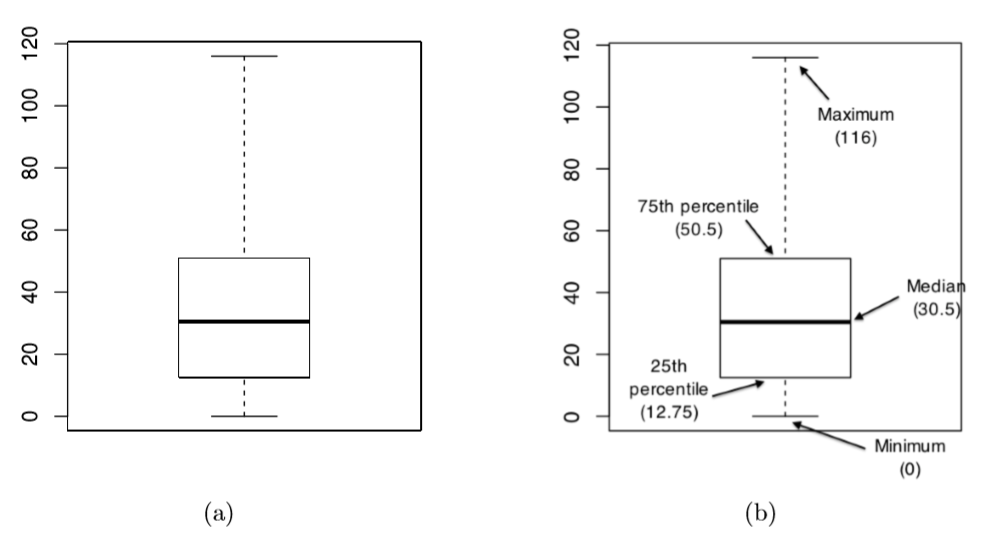
\includegraphics[width=13.64in]{./rbook-master/img/graphics2/boxplot1} \caption{A basic boxplot (panel a), plus the same plot with annotations added to explain what aspect of the data set each part of the boxplot corresponds to (panel b).}\label{fig:boxplot1}
\end{figure}

Another alternative to histograms is a \textbf{\emph{boxplot}},
sometimes called a ``box and whiskers'' plot. Like histograms, they're
most suited to interval or ratio scale data. The idea behind a boxplot
is to provide a simple visual depiction of the median, the interquartile
range, and the range of the data. And because they do so in a fairly
compact way, boxplots have become a very popular statistical graphic,
especially during the exploratory stage of data analysis when you're
trying to understand the data yourself. Let's have a look at how they
work, again using the \texttt{afl.margins} data as our example. Firstly,
let's actually calculate these numbers ourselves using the
\texttt{summary()} function:\footnote{R being what it is, it's no great
  surprise that there's also a \texttt{fivenum()} function that does
  much the same thing.}

\begin{verbatim}
> summary( afl.margins )
   Min. 1st Qu.  Median    Mean 3rd Qu.    Max. 
   0.00   12.75   30.50   35.30   50.50  116.00 
\end{verbatim}

So how does a boxplot capture these numbers? The easiest way to describe
what a boxplot looks like is just to draw one. The function for doing
this in R is (surprise, surprise) \texttt{boxplot()}. As always there's
a lot of optional arguments that you can specify if you want, but for
the most part you can just let R choose the defaults for you. That said,
I'm going to override one of the defaults to start with by specifying
the \texttt{range} option, but for the most part you won't want to do
this (I'll explain why in a minute). With that as preamble, let's try
the following command:

\begin{Shaded}
\begin{Highlighting}[]
\KeywordTok{boxplot}\NormalTok{( }\DataTypeTok{x =}\NormalTok{ afl.margins, }\DataTypeTok{range =} \DecValTok{100}\NormalTok{ )}
\end{Highlighting}
\end{Shaded}

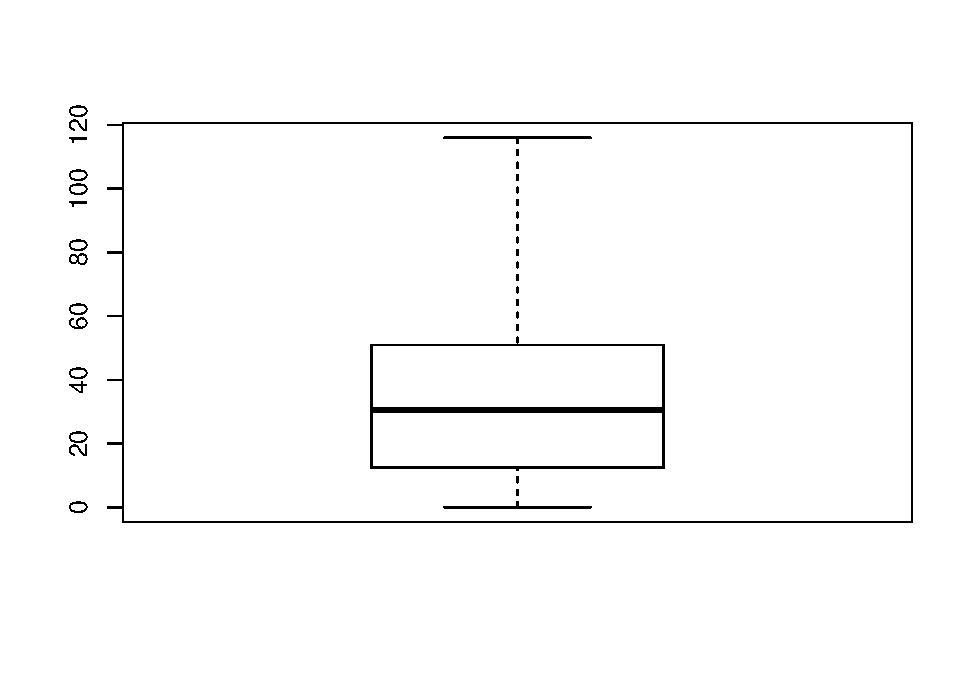
\includegraphics{navarro2_files/figure-latex/boxplot1a-1.pdf}

What R draws is shown in Figure \ref{fig:boxplot1a}, the most basic
boxplot possible. When you look at this plot, this is how you should
interpret it: the thick line in the middle of the box is the median; the
box itself spans the range from the 25th percentile to the 75th
percentile; and the ``whiskers'' cover the full range from the minimum
value to the maximum value. This is summarised in the annotated plot in
Figure \ref{fig:boxplot1b}.

In practice, this isn't quite how boxplots usually work. In most
applications, the ``whiskers'' don't cover the full range from minimum
to maximum. Instead, they actually go out to the most extreme data point
that doesn't exceed a certain bound. By default, this value is 1.5 times
the interquartile range, corresponding to a \texttt{range} value of 1.5.
Any observation whose value falls outside this range is plotted as a
circle instead of being covered by the whiskers, and is commonly
referred to as an \textbf{\emph{outlier}}. For our AFL margins data,
there is one observation (a game with a margin of 116 points) that falls
outside this range. As a consequence, the upper whisker is pulled back
to the next largest observation (a value of 108), and the observation at
116 is plotted as a circle. This is illustrated in Figure
@ref(fig:boxplot2a. Since the default value is \texttt{range\ =\ 1.5} we
can draw this plot using the simple command

\begin{Shaded}
\begin{Highlighting}[]
\KeywordTok{boxplot}\NormalTok{( afl.margins )}
\end{Highlighting}
\end{Shaded}

\begin{figure}
\centering
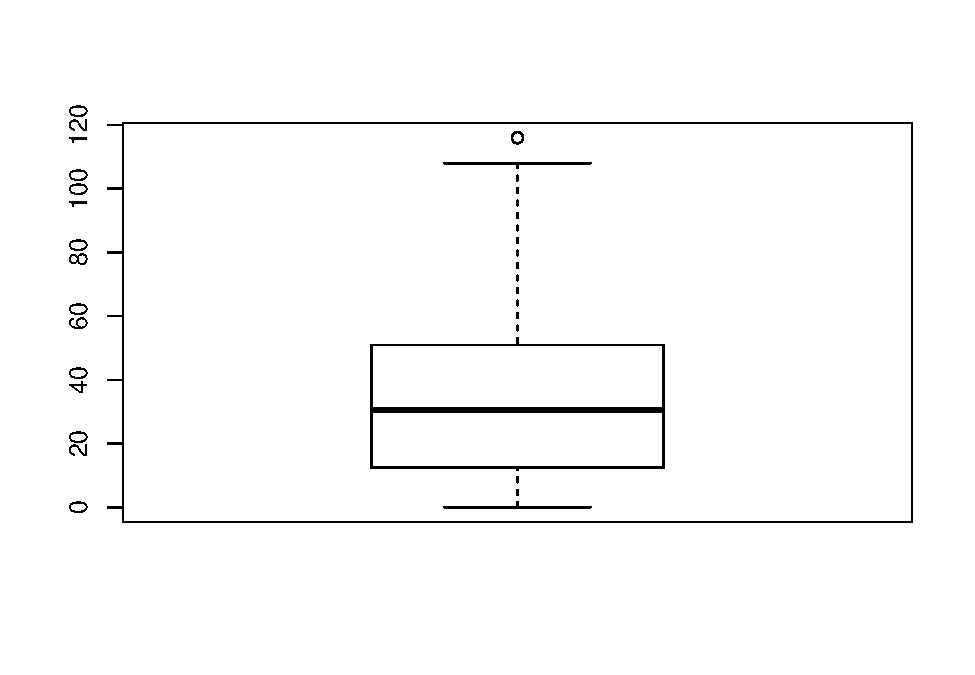
\includegraphics{navarro2_files/figure-latex/boxplot2a-1.pdf}
\caption{\label{fig:boxplot2a}By default, R will only extent the whiskers a
distance of 1.5 times the interquartile range, and will plot any points
that fall outside that range separately}
\end{figure}

\subsection{Visual style of your
boxplot}\label{visual-style-of-your-boxplot}

I'll talk a little more about the relationship between boxplots and
outliers in the Section \ref{sec:boxplotoutliers}, but before I do let's
take the time to clean this figure up. Boxplots in R are extremely
customisable. In addition to the usual range of graphical parameters
that you can tweak to make the plot look nice, you can also exercise
nearly complete control over every element to the plot. Consider the
boxplot in Figure \ref{fig:boxplot2b}: in this version of the plot, not
only have I added labels (\texttt{xlab}, \texttt{ylab}) and removed the
stupid border (\texttt{frame.plot}), I've also dimmed all of the
graphical elements of the boxplot except the central bar that plots the
median (\texttt{border}) so as to draw more attention to the median
rather than the rest of the boxplot.

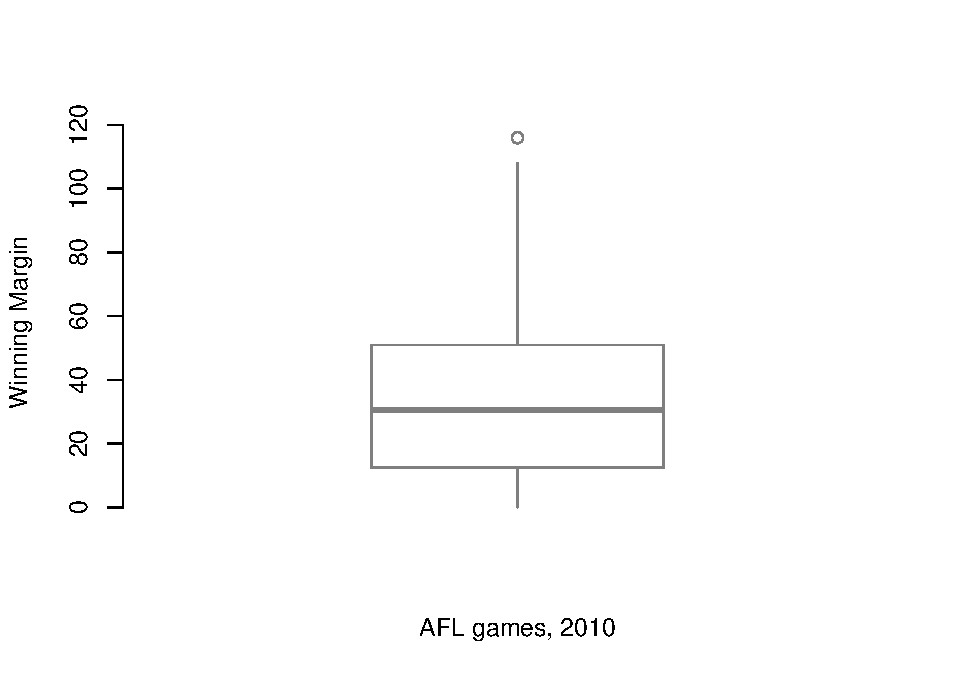
\includegraphics{navarro2_files/figure-latex/boxplot2b-1.pdf}

You've seen all these options in previous sections in this chapter, so
hopefully those customisations won't need any further explanation.
However, I've done two new things as well: I've deleted the cross-bars
at the top and bottom of the whiskers (known as the ``staples'' of the
plot), and converted the whiskers themselves to solid lines. The
arguments that I used to do this are called by the ridiculous names of
\texttt{staplewex} and \texttt{whisklty},\footnote{I realise there's a
  kind of logic to the way R names are constructed, but they still sound
  dumb. When I typed this sentence, all I could think was that it
  sounded like the name of a kids movie if it had been written by Lewis
  Carroll: ``The frabjous gambolles of Staplewex and Whisklty'' or
  something along those lines.} and I'll explain these in a moment.

But first, here's the actual command I used to draw this figure:

\begin{verbatim}
> boxplot( x = afl.margins,           # the data
+          xlab = "AFL games, 2010",  # x-axis label
+          ylab = "Winning Margin",   # y-axis label
+          border = "grey50",         # dim the border of the box
+          frame.plot = FALSE,        # don't draw a frame
+          staplewex = 0,             # don't draw staples
+          whisklty = 1               # solid line for whisker 
+ )
\end{verbatim}

Overall, I think the resulting boxplot is a huge improvement in visual
design over the default version. In my opinion at least, there's a
fairly minimalist aesthetic that governs good statistical graphics.
Ideally, every visual element that you add to a plot should convey part
of the message. If your plot includes things that don't actually help
the reader learn anything new, you should consider removing them.
Personally, I can't see the point of the cross-bars on a standard
boxplot, so I've deleted them.

Okay, what commands can we use to customise the boxplot? If you type
\texttt{?boxplot} and flick through the help documentation, you'll
notice that it does mention \texttt{staplewex} as an argument, but
there's no mention of \texttt{whisklty}. The reason for this is that the
function that handles the drawing is called \texttt{bxp()}, so if you
type \texttt{?bxp} all the gory details appear. Here's the short
summary. In order to understand why these arguments have such stupid
names, you need to recognise that they're put together from two
components. The first part of the argument name specifies one part of
the box plot: \texttt{staple} refers to the staples of the plot (i.e.,
the cross-bars), and \texttt{whisk} refers to the whiskers. The second
part of the name specifies a graphical parameter: \texttt{wex} is a
width parameter, and \texttt{lty} is a line type parameter. The parts of
the plot you can customise are:

\begin{itemize}
\tightlist
\item
  \texttt{box}. The box that covers the interquartile range.
\item
  \texttt{med}. The line used to show the median.
\item
  \texttt{whisk}. The vertical lines used to draw the whiskers.
\item
  \texttt{staple}. The cross bars at the ends of the whiskers.
\item
  \texttt{out}. The points used to show the outliers.
\end{itemize}

The actual graphical parameters that you might want to specify are
slightly different for each visual element, just because they're
different shapes from each other. As a consequence, the following
options are available:

\begin{itemize}
\tightlist
\item
  \emph{Width expansion:} \texttt{boxwex,\ staplewex,\ outwex}. These
  are scaling factors that govern the width of various parts of the
  plot. The default scaling factor is (usually) 0.8 for the box, and 0.5
  for the other two. Note that in the case of the outliers this
  parameter is meaningless unless you decide to draw lines plotting the
  outliers rather than use points.
\item
  \emph{Line type:}
  \texttt{boxlty,\ medlty,\ whisklty,\ staplelty,\ outlty}. These govern
  the line type for the relevant elements. The values for this are
  exactly the same as those used for the regular \texttt{lty} parameter,
  with two exceptions. There's an additional option where you can set
  \texttt{medlty\ =\ "blank"} to suppress the median line completely
  (useful if you want to draw a point for the median rather than plot a
  line). Similarly, by default the outlier line type is set to
  \texttt{outlty\ =\ "blank"}, because the default behaviour is to draw
  outliers as points instead of lines.
\item
  \emph{Line width:}
  \texttt{boxlwd,\ medlwd,\ whisklwd,\ staplelwd,\ outlwd}. These govern
  the line widths for the relevant elements, and behave the same way as
  the regular \texttt{lwd} parameter. The only thing to note is that the
  default value for \texttt{medlwd} value is three times the value of
  the others.
\item
  \emph{Line colour:}
  \texttt{boxcol,\ medcol,\ whiskcol,\ staplecol,\ outcol}. These govern
  the colour of the lines used to draw the relevant elements. Specify a
  colour in the same way that you usually do.
\item
  \emph{Fill colour:} \texttt{boxfill}. What colour should we use to
  fill the box?
\item
  \emph{Point character:} \texttt{medpch,\ outpch}. These behave like
  the regular \texttt{pch} parameter used to select the plot character.
  Note that you can set \texttt{outpch\ =\ NA} to stop R from plotting
  the outliers at all, and you can also set \texttt{medpch\ =\ NA} to
  stop it from drawing a character for the median (this is the default!)
\item
  \emph{Point expansion:} \texttt{medcex,\ outcex}. Size parameters for
  the points used to plot medians and outliers. These are only
  meaningful if the corresponding points are actually plotted. So for
  the default boxplot, which includes outlier points but uses a line
  rather than a point to draw the median, only the \texttt{outcex}
  parameter is meaningful.
\item
  \emph{Background colours:} \texttt{medbg,\ outbg}. Again, the
  background colours are only meaningful if the points are actually
  plotted.
\end{itemize}

Taken as a group, these parameters allow you almost complete freedom to
select the graphical style for your boxplot that you feel is most
appropriate to the data set you're trying to describe. That said, when
you're first starting out there's no shame in using the default
settings! But if you want to master the art of designing beautiful
figures, it helps to try playing around with these parameters to see
what works and what doesn't. Finally, I should mention a few other
arguments that you might want to make use of:

\begin{itemize}
\tightlist
\item
  \texttt{horizontal}. Set this to \texttt{TRUE} to display the plot
  horizontally rather than vertically.
\item
  \texttt{varwidth}. Set this to \texttt{TRUE} to get R to scale the
  width of each box so that the areas are proportional to the number of
  observations that contribute to the boxplot. This is only useful if
  you're drawing multiple boxplots at once (see Section
  \ref{multipleboxplots}.
\item
  \texttt{show.names}. Set this to \texttt{TRUE} to get R to attach
  labels to the boxplots.
\item
  \texttt{notch}. If you set \texttt{notch\ =\ TRUE}, R will draw little
  notches in the sides of each box. If the notches of two boxplots don't
  overlap, then there is a ``statistically significant'' difference
  between the corresponding medians. If you haven't read Chapter
  \ref{hypothesistesting}, ignore this argument -- we haven't discussed
  statistical significance, so this doesn't mean much to you. I'm
  mentioning it only because you might want to come back to the topic
  later on. (see also the \texttt{notch.frac} option when you type
  \texttt{?bxp}).
\end{itemize}

\subsection{Using box plots to detect outliers}\label{boxplotoutliers}

Because the boxplot automatically (unless you change the \texttt{range}
argument) separates out those observations that lie within a certain
range, people often use them as an informal method for detecting
\textbf{\emph{outliers}}: observations that are ``suspiciously'' distant
from the rest of the data. Here's an example. Suppose that I'd drawn the
boxplot for the AFL margins data, and it came up looking like Figure
\ref{fig:boxplotoutlier}.

\begin{figure}
\centering
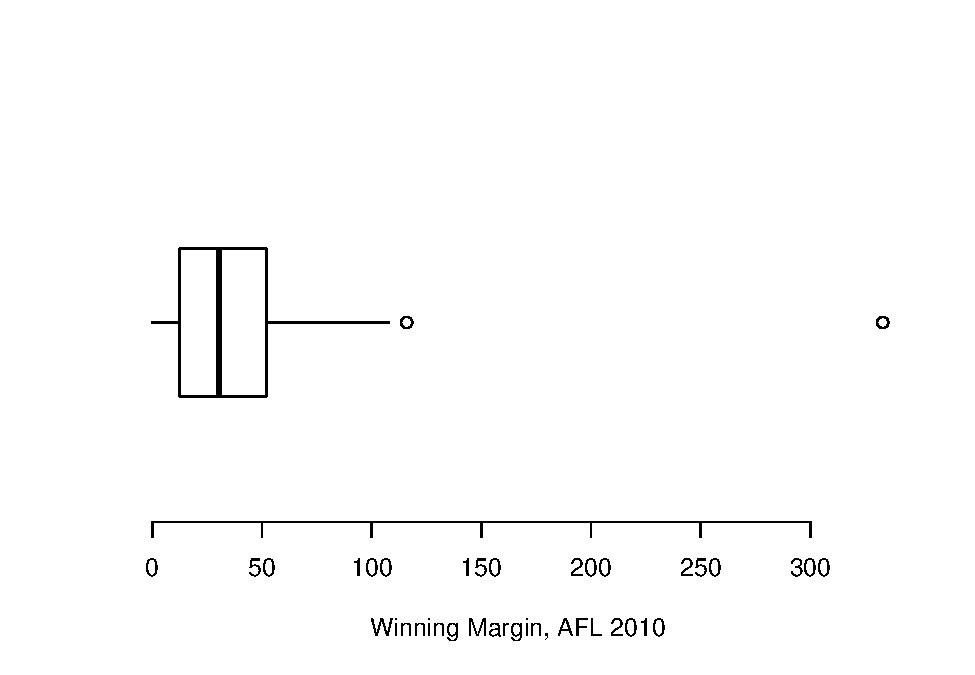
\includegraphics{navarro2_files/figure-latex/boxplotoutlier-1.pdf}
\caption{\label{fig:boxplotoutlier}A boxplot showing one very suspicious
outlier! I've drawn this plot in a similar, minimalist style to the one
in Figure \ref{fig:boxplot2b}, but I've used the \texttt{horizontal}
argument to draw it sideways in order to save space.}
\end{figure}

It's pretty clear that something funny is going on with one of the
observations. Apparently, there was one game in which the margin was
over 300 points! That doesn't sound right to me. Now that I've become
suspicious, it's time to look a bit more closely at the data. One
function that can be handy for this is the \texttt{which()} function; it
takes as input a vector of logicals, and outputs the indices of the
\texttt{TRUE} cases. This is particularly useful in the current context
because it lets me do this:

\begin{verbatim}
> suspicious.cases <- afl.margins > 300
> which( suspicious.cases )
[1] 137
\end{verbatim}

although in real life I probably wouldn't bother creating the
\texttt{suspicious.cases} variable: I'd just cut out the middle man and
use a command like \texttt{which(\ afl.margins\ \textgreater{}\ 300\ )}.
In any case, what this has done is shown me that the outlier corresponds
to game 137. Then, I find the recorded margin for that game:

\begin{verbatim}
> afl.margins[137]
[1] 333
\end{verbatim}

Hm. That definitely doesn't sound right. So then I go back to the
original data source (the internet!) and I discover that the actual
margin of that game was 33 points. Now it's pretty clear what happened.
Someone must have typed in the wrong number. Easily fixed, just by
typing \texttt{afl.margins{[}137{]}\ \textless{}-\ 33}. While this might
seem like a silly example, I should stress that this kind of thing
actually happens a lot. Real world data sets are often riddled with
stupid errors, especially when someone had to type something into a
computer at some point. In fact, there's actually a name for this phase
of data analysis, since in practice it can waste a huge chunk of our
time: \textbf{\emph{data cleaning}}. It involves searching for typos,
missing data and all sorts of other obnoxious errors in raw data
files.\footnote{Sometimes it's convenient to have the boxplot
  automatically label the outliers for you. The original
  \texttt{boxplot()} function doesn't allow you to do this; however, the
  \texttt{Boxplot()} function in the \texttt{car} package does. The
  design of the \texttt{Boxplot()} function is very similar to
  \texttt{boxplot()}. It just adds a few new arguments that allow you to
  tweak the labelling scheme. I'll leave it to the reader to check this
  out.}

What about the real data? Does the value of 116 constitute a funny
observation not? Possibly. As it turns out the game in question was
Fremantle v Hawthorn, and was played in round 21 (the second last home
and away round of the season). Fremantle had already qualified for the
final series and for them the outcome of the game was irrelevant; and
the team decided to rest several of their star players. As a
consequence, Fremantle went into the game severely underpowered. In
contrast, Hawthorn had started the season very poorly but had ended on a
massive winning streak, and for them a win could secure a place in the
finals. With the game played on Hawthorn's home turf\footnote{Sort of.
  The game was played in Launceston, which is a de facto home away from
  home for Hawthorn.} and with so many unusual factors at play, it is
perhaps no surprise that Hawthorn annihilated Fremantle by 116 points.
Two weeks later, however, the two teams met again in an elimination
final on Fremantle's home ground, and Fremantle won comfortably by 30
points.\footnote{Contrast this situation with the next largest winning
  margin in the data set, which was Geelong's 108 point demolition of
  Richmond in round 6 at their home ground, Kardinia Park. Geelong have
  been one of the most dominant teams over the last several years, a
  period during which they strung together an incredible 29-game winning
  streak at Kardinia Park. Richmond have been useless for several years.
  This is in no meaningful sense an outlier. Geelong have been winning
  by these margins (and Richmond losing by them) for quite some time.
  Frankly I'm surprised that the result wasn't more lopsided: as
  happened to Melbourne in 2011 when Geelong won by a modest 186 points.}

So, should we exclude the game from subsequent analyses? If this were a
psychology experiment rather than an AFL season, I'd be quite tempted to
exclude it because there's pretty strong evidence that Fremantle weren't
really trying very hard: and to the extent that my research question is
based on an assumption that participants are genuinely trying to do the
task. On the other hand, in a lot of studies we're actually interested
in seeing the full range of possible behaviour, and that includes
situations where people decide not to try very hard: so excluding that
observation would be a bad idea. In the context of the AFL data, a
similar distinction applies. If I'd been trying to make tips about who
would perform well in the finals, I would have (and in fact did)
disregard the Round 21 massacre, because it's way too misleading. On the
other hand, if my interest is solely in the home and away season itself,
I think it would be a shame to throw away information pertaining to one
of the most distinctive (if boring) games of the year. In other words,
the decision about whether to include outliers or exclude them depends
heavily on \emph{why} you think the data look they way they do, and what
you want to use the data \emph{for}. Statistical tools can provide an
automatic method for suggesting candidates for deletion, but you really
need to exercise good judgment here. As I've said before, R is a
mindless automaton. It doesn't watch the footy, so it lacks the broader
context to make an informed decision. You are \emph{not} a mindless
automaton, so you should exercise judgment: if the outlier looks
legitimate to you, then keep it. In any case, I'll return to the topic
again in Section \ref{regressiondiagnostics}, so let's return to our
discussion of how to draw boxplots.

\subsection{Drawing multiple boxplots}\label{multipleboxplots}

One last thing. What if you want to draw multiple boxplots at once?
Suppose, for instance, I wanted separate boxplots showing the AFL
margins not just for 2010, but for every year between 1987 and 2010. To
do that, the first thing we'll have to do is find the data. These are
stored in the \texttt{aflsmall2.Rdata} file. So let's load it and take a
quick peek at what's inside:

\begin{verbatim}
> load( "aflsmall2.Rdata" )
> who( TRUE )
   -- Name --   -- Class --   -- Size --
   afl2         data.frame    4296 x 2  
    $margin     numeric       4296      
    $year       numeric       4296     
\end{verbatim}

Notice that \texttt{afl2} data frame is pretty big. It contains 4296
games, which is far more than I want to see printed out on my computer
screen. To that end, R provides you with a few useful functions to print
out only a few of the row in the data frame. The first of these is
\texttt{head()} which prints out the first 6 rows, of the data frame,
like this:

\begin{verbatim}
> head( afl2 )
  margin year
1     33 1987
2     59 1987
3     45 1987
4     91 1987
5     39 1987
6      1 1987
\end{verbatim}

You can also use the \texttt{tail()} function to print out the last 6
rows. The \texttt{car} package also provides a handy little function
called \texttt{some()} which prints out a random subset of the rows.

In any case, the important thing is that we have the \texttt{afl2} data
frame which contains the variables that we're interested in. What we
want to do is have R draw boxplots for the \texttt{margin} variable,
plotted separately for each separate \texttt{year}. The way to do this
using the \texttt{boxplot()} function is to input a \texttt{formula}
rather than a variable as the input. In this case, the formula we want
is \texttt{margin\ \textasciitilde{}\ year}. So our boxplot command now
looks like this:
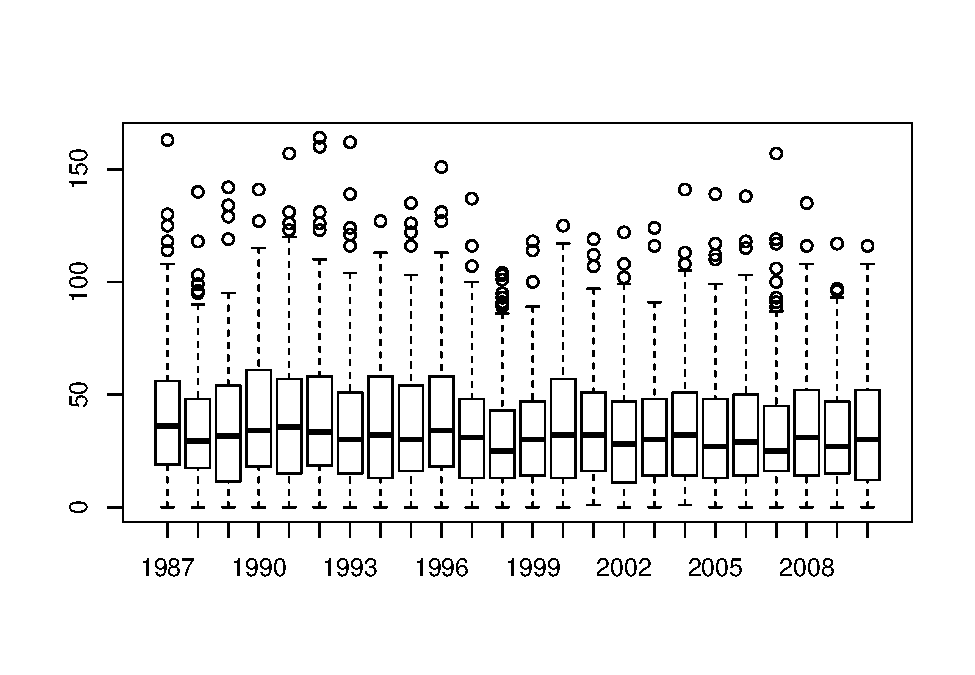
\includegraphics{navarro2_files/figure-latex/multipleboxplots-1.pdf}

The result is shown in Figure \ref{fig:multipleboxplots}.\footnote{Actually,
  there's other ways to do this. If the input argument \texttt{x} is a
  list object (see Section \ref{lists}, the \texttt{boxplot()} function
  will draw a separate boxplot for each variable in that list.
  Relatedly, since the \texttt{plot()} function -- which we'll discuss
  shortly -- is a generic (see Section \ref{generics}, you might not be
  surprised to learn that one of its special cases is a boxplot:
  specifically, if you use \texttt{plot()} where the first argument
  \texttt{x} is a factor and the second argument \texttt{y} is numeric,
  then the result will be a boxplot, showing the values in \texttt{y},
  with a separate boxplot for each level. For instance, something like
  \texttt{plot(x\ =\ afl2\textbackslash{}\$year,\ y\ =\ afl2\textbackslash{}\$margin)}
  would work.} Even this, the default version of the plot, gives a sense
of why it's sometimes useful to choose boxplots instead of histograms.
Even before taking the time to turn this basic output into something
more readable, it's possible to get a good sense of what the data look
like from year to year without getting overwhelmed with too much detail.
Now imagine what would have happened if I'd tried to cram 24 histograms
into this space: no chance at all that the reader is going to learn
anything useful.

\begin{figure}
\centering
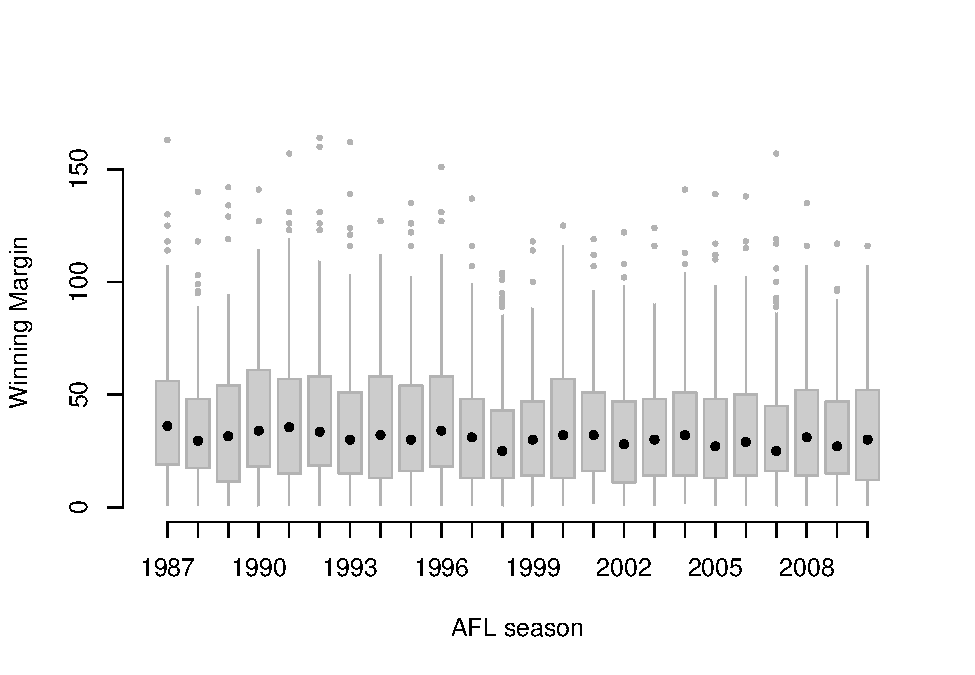
\includegraphics{navarro2_files/figure-latex/multipleboxplots2-1.pdf}
\caption{\label{fig:multipleboxplots2}A cleaned up version of Figure
\ref{fig:multipleboxplots}. Notice that I've used a very minimalist
design for the boxplots, so as to focus the eye on the medians. I've
also converted the medians to solid dots, to convey a sense that year to
year variation in the median should be thought of as a single coherent
plot (similar to what we did when plotting the \texttt{Fibonacci}
variable earlier). The size of outliers has been shrunk, because they
aren't actually very interesting. In contrast, I've added a fill colour
to the boxes, to make it easier to look at the trend in the
interquartile range across years.}
\end{figure}

That being said, the default boxplot leaves a great deal to be desired
in terms of visual clarity. The outliers are too visually prominent, the
dotted lines look messy, and the interesting content (i.e., the
behaviour of the median and the interquartile range across years) gets a
little obscured. Fortunately, this is easy to fix, since we've already
covered a lot of tools you can use to customise your output. After
playing around with several different versions of the plot, the one I
settled on is shown in Figure \ref{fig:multipleboxplots2}. The command I
used to produce it is long, but not complicated:

\begin{verbatim}
>  boxplot( formula =  margin ~ year,   # the formula
+           data = afl2,                # the data set
+           xlab = "AFL season",        # x axis label
+           ylab = "Winning Margin",    # y axis label
+           frame.plot = FALSE,         # don't draw a frame
+           staplewex = 0,              # don't draw staples
+           staplecol = "white",        # (fixes a tiny display issue)
+           boxwex = .75,               # narrow the boxes slightly
+           boxfill = "grey80",         # lightly shade the boxes
+           whisklty = 1,               # solid line for whiskers 
+           whiskcol = "grey70",        # dim the whiskers
+           boxcol = "grey70",          # dim the box borders
+           outcol = "grey70",          # dim the outliers
+           outpch = 20,                # outliers as solid dots
+           outcex = .5,                # shrink the outliers
+           medlty = "blank",           # no line for the medians
+           medpch = 20,                # instead, draw solid dots
+           medlwd = 1.5                # make them larger
+ )
\end{verbatim}

Of course, given that the command is that long, you might have guessed
that I didn't spend ages typing all that rubbish in over and over again.
Instead, I wrote a script, which I kept tweaking until it produced the
figure that I wanted. We'll talk about scripts later in Section
\ref{scripts}, but given the length of the command I thought I'd remind
you that there's an easier way of trying out different commands than
typing them all in over and over.

\section{Scatterplots}\label{scatterplots}

\textbf{\emph{Scatterplots}} are a simple but effective tool for
visualising data. We've already seen scatterplots in this chapter, when
using the \texttt{plot()} function to draw the \texttt{Fibonacci}
variable as a collection of dots (Section \ref{introplotting}. However,
for the purposes of this section I have a slightly different notion in
mind. Instead of just plotting one variable, what I want to do with my
scatterplot is display the relationship between \emph{two} variables,
like we saw with the figures in the section on correlation (Section
\ref{correl}. It's this latter application that we usually have in mind
when we use the term ``scatterplot''. In this kind of plot, each
observation corresponds to one dot: the horizontal location of the dot
plots the value of the observation on one variable, and the vertical
location displays its value on the other variable. In many situations
you don't really have a clear opinions about what the \emph{causal}
relationship is (e.g., does A cause B, or does B cause A, or does some
other variable C control both A and B). If that's the case, it doesn't
really matter which variable you plot on the x-axis and which one you
plot on the y-axis. However, in many situations you do have a pretty
strong idea which variable you think is most likely to be causal, or at
least you have some suspicions in that direction. If so, then it's
conventional to plot the cause variable on the x-axis, and the effect
variable on the y-axis. With that in mind, let's look at how to draw
scatterplots in R, using the same \texttt{parenthood} data set (i.e.
\texttt{parenthood.Rdata}) that I used when introducing the idea of
correlations.

\textbackslash{}begin\{figure\}
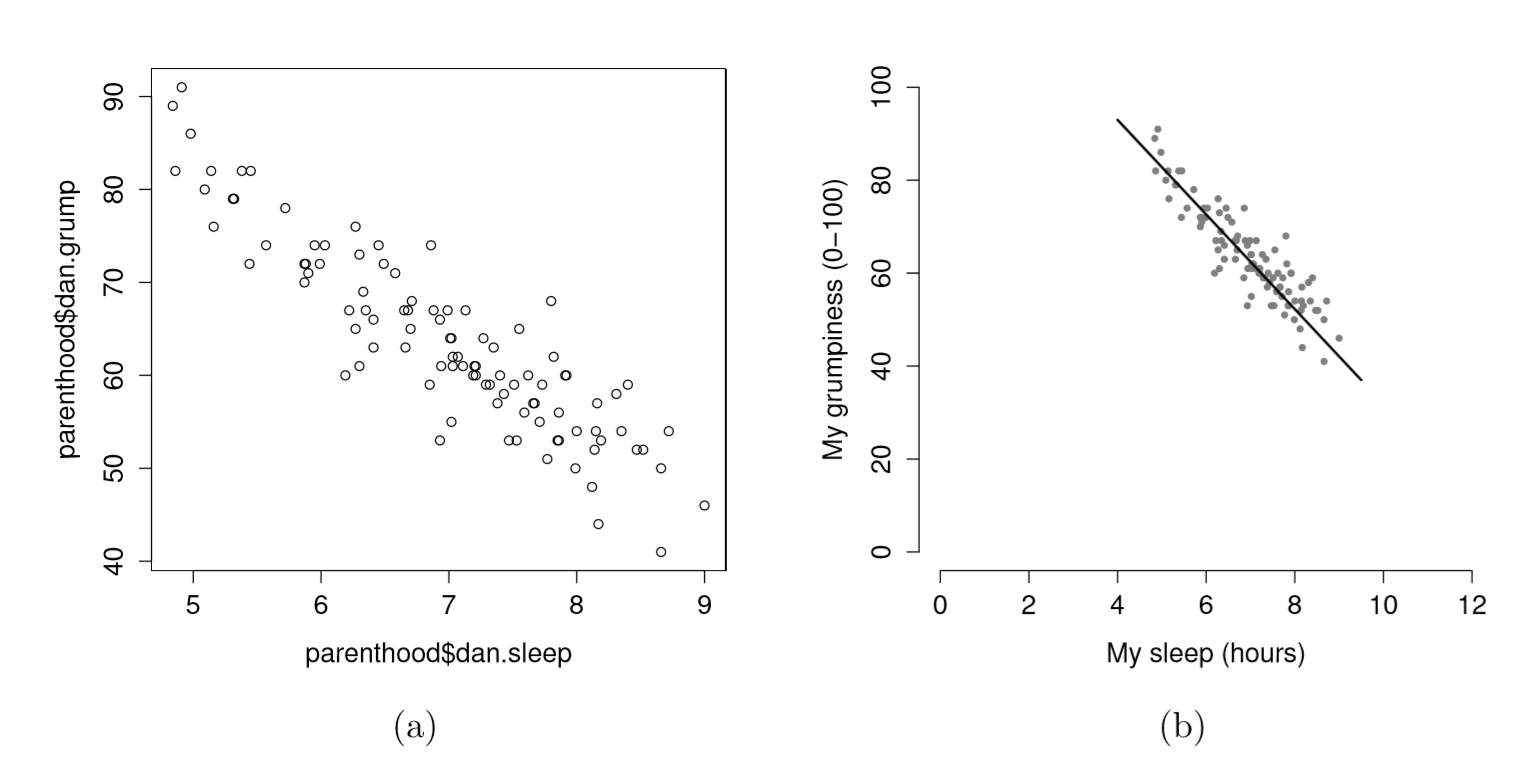
\includegraphics[width=21.35in]{./rbook-master/img/graphics2/scatter1}
\textbackslash{}caption\{\{Two different scatterplots: (a) the default
scatterplot that R produces, (b) one that makes use of several options
for fancier display.\}\label{fig:scatter} \textbackslash{}end\{figure\}

Suppose my goal is to draw a scatterplot displaying the relationship
between the amount of sleep that I get (\texttt{dan.sleep}) and how
grumpy I am the next day (\texttt{dan.grump}). As you might expect given
our earlier use of \texttt{plot()} to display the \texttt{Fibonacci}
data, the function that we use is the \texttt{plot()} function, but
because it's a generic function all the hard work is still being done by
the \texttt{plot.default()} function. In any case, there are two
different ways in which we can get the plot that we're after. The first
way is to specify the name of the variable to be plotted on the
\texttt{x} axis and the variable to be plotted on the \texttt{y} axis.
When we do it this way, the command looks like this:

\begin{Shaded}
\begin{Highlighting}[]
\KeywordTok{plot}\NormalTok{( }\DataTypeTok{x =}\NormalTok{ parenthood}\OperatorTok{$}\NormalTok{dan.sleep,   }\CommentTok{# data on the x-axis}
      \DataTypeTok{y =}\NormalTok{ parenthood}\OperatorTok{$}\NormalTok{dan.grump    }\CommentTok{# data on the y-axis}
\NormalTok{ )  }
\end{Highlighting}
\end{Shaded}

\begin{figure}
\centering
\includegraphics{navarro2_files/figure-latex/scattera-1.pdf}
\caption{\label{fig:scattera}the default scatterplot that R produces}
\end{figure}

The second way do to it is to use a ``formula and data frame'' format,
but I'm going to avoid using it.\footnote{The reason is that there's an
  annoying design flaw in the way the \texttt{plot()} function handles
  this situation. The problem is that the \texttt{plot.formula()}
  function uses different names to for the arguments than the
  \texttt{plot()} function expects. As a consequence, you can't specify
  the formula argument by name. If you just specify a formula as the
  first argument without using the name it works fine, because the
  \texttt{plot()} function thinks the formula corresponds to the
  \texttt{x} argument, and the \texttt{plot.formula()} function thinks
  it corresponds to the \texttt{formula} argument; and surprisingly,
  everything works nicely. But the moment that you, the user, tries to
  be unambiguous about the name, one of those two functions is going to
  cry.} For now, let's just stick with the \texttt{x} and \texttt{y}
version. If we do this, the result is the very basic scatterplot shown
in Figure \ref{fig:scattera}. This serves fairly well, but there's a few
customisations that we probably want to make in order to have this work
properly. As usual, we want to add some labels, but there's a few other
things we might want to do as well. Firstly, it's sometimes useful to
rescale the plots. In Figure \ref{fig:scattera} R has selected the
scales so that the data fall neatly in the middle. But, in this case, we
happen to know that the grumpiness measure falls on a scale from 0 to
100, and the hours slept falls on a natural scale between 0 hours and
about 12 or so hours (the longest I can sleep in real life). So the
command I might use to draw this is:

\begin{Shaded}
\begin{Highlighting}[]
\KeywordTok{plot}\NormalTok{( }\DataTypeTok{x =}\NormalTok{ parenthood}\OperatorTok{$}\NormalTok{dan.sleep,         }\CommentTok{# data on the x-axis}
       \DataTypeTok{y =}\NormalTok{ parenthood}\OperatorTok{$}\NormalTok{dan.grump,         }\CommentTok{# data on the y-axis}
       \DataTypeTok{xlab =} \StringTok{"My sleep (hours)"}\NormalTok{,        }\CommentTok{# x-axis label}
       \DataTypeTok{ylab =} \StringTok{"My grumpiness (0-100)"}\NormalTok{,   }\CommentTok{# y-axis label}
       \DataTypeTok{xlim =} \KeywordTok{c}\NormalTok{(}\DecValTok{0}\NormalTok{,}\DecValTok{12}\NormalTok{),                   }\CommentTok{# scale the x-axis}
       \DataTypeTok{ylim =} \KeywordTok{c}\NormalTok{(}\DecValTok{0}\NormalTok{,}\DecValTok{100}\NormalTok{),                  }\CommentTok{# scale the y-axis}
       \DataTypeTok{pch =} \DecValTok{20}\NormalTok{,                         }\CommentTok{# change the plot type}
       \DataTypeTok{col =} \StringTok{"gray50"}\NormalTok{,                   }\CommentTok{# dim the dots slightly}
       \DataTypeTok{frame.plot =} \OtherTok{FALSE}                \CommentTok{# don't draw a box}
\NormalTok{ )}
\end{Highlighting}
\end{Shaded}

This command produces the scatterplot in Figure \ref{fig:scatterb}, or
at least very nearly. What it doesn't do is draw the line through the
middle of the points. Sometimes it can be very useful to do this, and I
can do so using \texttt{lines()}, which is a low level plotting
function. Better yet, the arguments that I need to specify are pretty
much the exact same ones that I use when calling the \texttt{plot()}
function. That is, suppose that I want to draw a line that goes from the
point (4,93) to the point (9.5,37). Then the \texttt{x} locations can be
specified by the vector \texttt{c(4,9.5)} and the \texttt{y} locations
correspond to the vector \texttt{c(93,37)}. In other words, I use this
command:

\begin{Shaded}
\begin{Highlighting}[]
\KeywordTok{plot}\NormalTok{( }\DataTypeTok{x =}\NormalTok{ parenthood}\OperatorTok{$}\NormalTok{dan.sleep,         }\CommentTok{# data on the x-axis}
       \DataTypeTok{y =}\NormalTok{ parenthood}\OperatorTok{$}\NormalTok{dan.grump,         }\CommentTok{# data on the y-axis}
       \DataTypeTok{xlab =} \StringTok{"My sleep (hours)"}\NormalTok{,        }\CommentTok{# x-axis label}
       \DataTypeTok{ylab =} \StringTok{"My grumpiness (0-100)"}\NormalTok{,   }\CommentTok{# y-axis label}
       \DataTypeTok{xlim =} \KeywordTok{c}\NormalTok{(}\DecValTok{0}\NormalTok{,}\DecValTok{12}\NormalTok{),                   }\CommentTok{# scale the x-axis}
       \DataTypeTok{ylim =} \KeywordTok{c}\NormalTok{(}\DecValTok{0}\NormalTok{,}\DecValTok{100}\NormalTok{),                  }\CommentTok{# scale the y-axis}
       \DataTypeTok{pch =} \DecValTok{20}\NormalTok{,                         }\CommentTok{# change the plot type}
       \DataTypeTok{col =} \StringTok{"gray50"}\NormalTok{,                   }\CommentTok{# dim the dots slightly}
       \DataTypeTok{frame.plot =} \OtherTok{FALSE}                \CommentTok{# don't draw a box}
\NormalTok{ )}
 \KeywordTok{lines}\NormalTok{( }\DataTypeTok{x =} \KeywordTok{c}\NormalTok{(}\DecValTok{4}\NormalTok{,}\FloatTok{9.5}\NormalTok{),   }\CommentTok{# the horizontal locations}
        \DataTypeTok{y =} \KeywordTok{c}\NormalTok{(}\DecValTok{93}\NormalTok{,}\DecValTok{37}\NormalTok{),   }\CommentTok{# the vertical locations}
        \DataTypeTok{lwd =} \DecValTok{2}         \CommentTok{# line width}
\NormalTok{ )}
\end{Highlighting}
\end{Shaded}

\includegraphics{navarro2_files/figure-latex/scatterb-1.pdf}

And when I do so, R plots the line over the top of the plot that I drew
using the previous command. In most realistic data analysis situations
you absolutely don't want to just guess where the line through the
points goes, since there's about a billion different ways in which you
can get R to do a better job. However, it does at least illustrate the
basic idea.

One possibility, if you do want to get R to draw nice clean lines
through the data for you, is to use the \texttt{scatterplot()} function
in the \texttt{car} package. Before we can use \texttt{scatterplot()} we
need to load the package:

\begin{verbatim}
> library( car )
\end{verbatim}

Having done so, we can now use the function. The command we need is this
one:

\begin{verbatim}
> scatterplot( dan.grump ~ dan.sleep,
+              data = parenthood, 
+              smooth = FALSE
+ )
\end{verbatim}

\begin{figure}
\centering
\includegraphics{navarro2_files/figure-latex/fancyscatter-1.pdf}
\caption{\label{fig:fancyscatter}A fancy scatterplot drawn using the
\texttt{scatterplot()} function in the \texttt{car} package.}
\end{figure}

The first two arguments should be familiar: the first input is a formula
\texttt{dan.grump\ \textasciitilde{}\ dan.sleep} telling R what
variables to plot,\footnote{You might be wondering why I haven't
  specified the argument name for the formula. The reason is that
  there's a bug in how the \texttt{scatterplot()} function is written:
  under the hood there's one function that expects the argument to be
  named \texttt{x} and another one that expects it to be called
  \texttt{formula}. I don't know why the function was written this way,
  but it's not an isolated problem: this particular kind of bug repeats
  itself in a couple of other functions (you'll see it again in Chapter
  \ref{ttest}. The solution in such cases is to omit the argument name:
  that way, one function ``thinks'' that you've specified \texttt{x} and
  the other one ``thinks'' you've specified \texttt{formula} and
  everything works the way it's supposed to. It's not a great state of
  affairs, I'll admit, but it sort of works.} and the second specifies a
\texttt{data} frame. The third argument \texttt{smooth} I've set to
\texttt{FALSE} to stop the \texttt{scatterplot()} function from drawing
a fancy ``smoothed'' trendline (since it's a bit confusing to
beginners). The scatterplot itself is shown in Figure
\ref{fig:fancyscatter}. As you can see, it's not only drawn the
scatterplot, but its also drawn boxplots for each of the two variables,
as well as a simple line of best fit showing the relationship between
the two variables.

\subsection{More elaborate options}\label{more-elaborate-options}

Often you find yourself wanting to look at the relationships between
several variables at once. One useful tool for doing so is to produce a
\textbf{\emph{scatterplot matrix}}, analogous to the correlation matrix.

\begin{verbatim}
> cor( x = parenthood ) # calculate correlation matrix
             dan.sleep  baby.sleep   dan.grump         day
dan.sleep   1.00000000  0.62794934 -0.90338404 -0.09840768
baby.sleep  0.62794934  1.00000000 -0.56596373 -0.01043394
dan.grump  -0.90338404 -0.56596373  1.00000000  0.07647926
day        -0.09840768 -0.01043394  0.07647926  1.00000000
\end{verbatim}

We can get a the corresponding scatterplot matrix by using the
\texttt{pairs()} function:\footnote{Yet again, we could have produced
  this output using the \texttt{plot()} function: when the \texttt{x}
  argument is a data frame containing numeric variables only, then the
  output is a scatterplot matrix. So, once again, what I could have done
  is just type \texttt{plot(\ parenthood\ )}.}

\begin{Shaded}
\begin{Highlighting}[]
\KeywordTok{pairs}\NormalTok{( }\DataTypeTok{x =}\NormalTok{ parenthood ) }\CommentTok{# draw corresponding scatterplot matrix  }
\end{Highlighting}
\end{Shaded}

\includegraphics{navarro2_files/figure-latex/pairs-1.pdf}

The output of the \texttt{pairs()} command is shown in Figure
\ref{fig:pairs}. An alternative way of calling the \texttt{pairs()}
function, which can be useful in some situations, is to specify the
variables to include using a one-sided formula. For instance, this

\begin{verbatim}
> pairs( formula = ~ dan.sleep + baby.sleep + dan.grump,
+        data = parenthood
+ )
\end{verbatim}

would produce a \(3 \times 3\) scatterplot matrix that only compare
\texttt{dan.sleep}, \texttt{dan.grump} and \texttt{baby.sleep}.
Obviously, the first version is much easier, but there are cases where
you really only want to look at a few of the variables, so it's nice to
use the formula interface.

\section{Bar graphs}\label{bargraph}

Another form of graph that you often want to plot is the
\textbf{\emph{bar graph}}. The main function that you can use in R to
draw them is the \texttt{barplot()} function.\footnote{Once again, it's
  worth noting the link to the generic \texttt{plot()} function. If the
  \texttt{x} argument to \texttt{plot()} is a factor (and no \texttt{y}
  argument is given), the result is a bar graph. So you could use
  \texttt{plot(\ afl.finalists\ )} and get the same output as
  \texttt{barplot(\ afl.finalists\ )}.} And to illustrate the use of the
function, I'll use the \texttt{finalists} variable that I introduced in
Section \ref{mode}. What I want to do is draw a bar graph that displays
the number of finals that each team has played in over the time spanned
by the \texttt{afl} data set. So, let's start by creating a vector that
contains this information. I'll use the \texttt{tabulate()} function to
do this (which will be discussed properly in Section
\ref{sec:freqtables}, since it creates a simple numeric vector:

\begin{verbatim}
> freq <- tabulate( afl.finalists )
> print( freq )
 [1] 26 25 26 28 32  0  6 39 27 28 28 17  6 24 26 39 24
\end{verbatim}

This isn't exactly the prettiest of frequency tables, of course. I'm
only doing it this way so that you can see the \texttt{barplot()}
function in it's ``purest'' form: when the input is just an ordinary
numeric vector. That being said, I'm obviously going to need the team
names to create some labels, so let's create a variable with those. I'll
do this using the \texttt{levels()} function, which outputs the names of
all the levels of a factor (see Section \ref{factors}:

\begin{verbatim}
> teams <- levels( afl.finalists )
> print( teams )
 [1] "Adelaide"         "Brisbane"         "Carlton"          "Collingwood"     
 [5] "Essendon"         "Fitzroy"          "Fremantle"        "Geelong"         
 [9] "Hawthorn"         "Melbourne"        "North Melbourne"  "Port Adelaide"   
[13] "Richmond"         "St Kilda"         "Sydney"           "West Coast"      
[17] "Western Bulldogs"
\end{verbatim}

Okay, so now that we have the information we need, let's draw our bar
graph. The main argument that you need to specify for a bar graph is the
\texttt{height} of the bars, which in our case correspond to the values
stored in the \texttt{freq} variable:

\begin{verbatim}
> barplot( height = freq )  # specifying the argument name (panel a)
> barplot( freq )   # the lazier version (panel a)
\end{verbatim}

Either of these two commands will produce the simple bar graph shown in
Figure \ref{fig:bar1a}.

\begin{figure}
\centering
\includegraphics{navarro2_files/figure-latex/bar1a-1.pdf}
\caption{\label{fig:bar1a}the simplest version of a bargraph, containing the
data but no labels}
\end{figure}

As you can see, R has drawn a pretty minimal plot. It doesn't have any
labels, obviously, because we didn't actually tell the
\texttt{barplot()} function what the labels are! To do this, we need to
specify the \texttt{names.arg} argument. The \texttt{names.arg} argument
needs to be a vector of character strings containing the text that needs
to be used as the label for each of the items. In this case, the
\texttt{teams} vector is exactly what we need, so the command we're
looking for is:

\begin{Shaded}
\begin{Highlighting}[]
    \KeywordTok{barplot}\NormalTok{( }\DataTypeTok{height =}\NormalTok{ freq, }\DataTypeTok{names.arg =}\NormalTok{ teams ) }
\end{Highlighting}
\end{Shaded}

\begin{figure}
\centering
\includegraphics{navarro2_files/figure-latex/bar1b-1.pdf}
\caption{\label{fig:bar1b}we've added the labels, but because the text runs
horizontally R only includes a few of them}
\end{figure}

This is an improvement, but not much of an improvement. R has only
included a few of the labels, because it can't fit them in the plot.
This is the same behaviour we saw earlier with the multiple-boxplot
graph in Figure \ref{fig:multipleboxplots}. However, in Figure
\ref{fig:multipleboxplots} it wasn't an issue: it's pretty obvious from
inspection that the two unlabelled plots in between 1987 and 1990 must
correspond to the data from 1988 and 1989. However, the fact that
\texttt{barplot()} has omitted the names of every team in between
Adelaide and Fitzroy is a lot more problematic.

The simplest way to fix this is to rotate the labels, so that the text
runs vertically not horizontally. To do this, we need to alter set the
\texttt{las} parameter, which I discussed briefly in Section
\ref{sec:introplotting}. What I'll do is tell R to rotate the text so
that it's always perpendicular to the axes (i.e., I'll set
\texttt{las\ =\ 2}). When I do that, as per the following
command\ldots{}

\begin{Shaded}
\begin{Highlighting}[]
    \KeywordTok{barplot}\NormalTok{(}\DataTypeTok{height =}\NormalTok{ freq,  }\CommentTok{# the frequencies}
            \DataTypeTok{names.arg =}\NormalTok{ teams,  }\CommentTok{# the label}
            \DataTypeTok{las =} \DecValTok{2}\NormalTok{)            }\CommentTok{# rotate the labels}
\end{Highlighting}
\end{Shaded}

\begin{figure}
\centering
\includegraphics{navarro2_files/figure-latex/bar1c-1.pdf}
\caption{\label{fig:bar1c}we've rotated the labels, but now the text is too
long to fit}
\end{figure}

\ldots{} the result is the bar graph shown in Figure \ref{fig:bar1c}.
We've fixed the problem, but we've created a new one: the axis labels
don't quite fit anymore. To fix this, we have to be a bit cleverer
again. A simple fix would be to use shorter names rather than the full
name of all teams, and in many situations that's probably the right
thing to do. However, at other times you really do need to create a bit
more space to add your labels, so I'll show you how to do that.

\subsection{\texorpdfstring{Changing global settings using
\texttt{par()}}{Changing global settings using par()}}\label{changing-global-settings-using-par}

Altering the margins to the plot is actually a somewhat more complicated
exercise than you might think. In principle it's a very simple thing to
do: the size of the margins is governed by a graphical parameter called
\texttt{mar}, so all we need to do is alter this parameter. First, let's
look at what the \texttt{mar} argument specifies. The \texttt{mar}
argument is a vector containing four numbers: specifying the amount of
space at the bottom, the left, the top and then the right. The units are
``number of
\texttt{lines\textquotesingle{}".\ The\ default\ value\ for}mar\texttt{is}c(5.1,
4.1, 4.1, 2.1)`, meaning that R leaves 5.1''lines" empty at the bottom,
4.1 lines on the left and the bottom, and only 2.1 lines on the right.
In order to make more room at the bottom, what I need to do is change
the first of these numbers. A value of 10.1 should do the trick.

So far this doesn't seem any different to the other graphical parameters
that we've talked about. However, because of the way that the
traditional graphics system in R works, you need to specify what the
margins will be \emph{before} calling your high-level plotting function.
Unlike the other cases we've see, you can't treat \texttt{mar} as if it
were just another argument in your plotting function. Instead, you have
to use the \texttt{par()} function to change the graphical parameters
beforehand, and only then try to draw your figure. In other words, the
first thing I would do is this:

\begin{verbatim}
> par( mar = c( 10.1, 4.1, 4.1, 2.1) )
\end{verbatim}

There's no visible output here, but behind the scenes R has changed the
graphical parameters associated with the current device (remember, in R
terminology all graphics are drawn onto a ``device''). Now that this is
done, we could use the exact same command as before, but this time you'd
see that the labels all fit, because R now leaves twice as much room for
the labels at the bottom. However, since I've now figured out how to get
the labels to display properly, I might as well play around with some of
the other options, all of which are things you've seen before:

\begin{figure}
\centering
\includegraphics{navarro2_files/figure-latex/bar1d-1.pdf}
\caption{\label{fig:bar1d}we fix this by expanding the margin at the bottom,
and add several other customisations to make the chart a bit nicer}
\end{figure}

\begin{Shaded}
\begin{Highlighting}[]
\KeywordTok{barplot}\NormalTok{( }\DataTypeTok{height =}\NormalTok{ freq,}
        \DataTypeTok{names.arg =}\NormalTok{ teams,}
        \DataTypeTok{las=}\DecValTok{2}\NormalTok{,}
        \DataTypeTok{ylab =} \StringTok{"Number of Finals"}\NormalTok{,}
        \DataTypeTok{main =} \StringTok{"Finals Played, 1987-2010"}\NormalTok{,  }
        \DataTypeTok{density =} \DecValTok{10}\NormalTok{,}
        \DataTypeTok{angle =} \DecValTok{20}\NormalTok{)}
\end{Highlighting}
\end{Shaded}

However, one thing to remember about the \texttt{par()} function is that
it doesn't just change the graphical parameters for the current
\emph{plot}. Rather, the changes pertain to any subsequent plot that you
draw onto the same \emph{device}. This might be exactly what you want,
in which case there's no problem. But if not, you need to reset the
graphical parameters to their original settings. To do this, you can
either close the device (e.g., close the window, or click the ``Clear
All'' button in the Plots panel in Rstudio) or you can reset the
graphical parameters to their original values, using a command like
this:

\begin{verbatim}
> par( mar = c(5.1, 4.1, 4.1, 2.1) )
\end{verbatim}

\section{Saving image files using R and Rstudio}\label{saveimage}

Hold on, you might be thinking. What's the good of being able to draw
pretty pictures in R if I can't save them and send them to friends to
brag about how awesome my data is? How do I save the picture? This is
another one of those situations where the easiest thing to do is to use
the RStudio tools.

If you're running R through Rstudio, then the easiest way to save your
image is to click on the ``Export'' button in the Plot panel (i.e., the
area in Rstudio where all the plots have been appearing). When you do
that you'll see a menu that contains the options ``Save Plot as PDF''
and ``Save Plot as Image''. Either version works. Both will bring up
dialog boxes that give you a few options that you can play with, but
besides that it's pretty simple.

This works pretty nicely for most situations. So, unless you're filled
with a burning desire to learn the low level details, feel free to skip
the rest of this section.

\subsection{The ugly details
(advanced)}\label{the-ugly-details-advanced}

As I say, the menu-based options should be good enough for most people
most of the time. However, one day you might want to be a bit more
sophisticated, and make use of R's image writing capabilities at a lower
level. In this section I'll give you a very basic introduction to this.
In all honesty, this barely scratches the surface, but it will help a
little bit in getting you started if you want to learn the details.

Okay, as I hinted earlier, whenever you're drawing pictures in R you're
deemed to be drawing \emph{to} a device of some kind. There are devices
that correspond to a figure drawn on screen, and there are devices that
correspond to graphics files that R will produce for you. For the
purposes of this section I'll assume that you're using the default
application in either Windows or Mac OS, not Rstudio. The reason for
this is that my experience with the graphical device provided by Rstudio
has led me to suspect that it still has a bunch on non-standard (or
possibly just undocumented) features, and so I don't quite trust that it
always does what I expect. I've no doubt they'll smooth it out later,
but I can honestly say that I don't quite get what's going on with the
\texttt{RStudioGD} device. In any case, we can ask R to list all of the
graphics devices that currently exist, simply by using the command
\texttt{dev.list()}. If there are no figure windows open, then you'll
see this:

\begin{verbatim}
> dev.list()
NULL
\end{verbatim}

which just means that R doesn't have any graphics devices open. However,
suppose if you've just drawn a histogram and you type the same command,
R will now give you a different answer. For instance, if you're using
Windows:

\begin{verbatim}
> hist( afl.margins )
> dev.list()
windows 
      2
\end{verbatim}

What this means is that there is one graphics device (device 2) that is
currently open, and it's a figure window. If you did the same thing on a
Mac, you get basically the same answer, except that the name of the
device would be \texttt{quartz} rather than \texttt{windows}. If you had
several graphics windows open (which, incidentally, you can do by using
the \texttt{dev.new()} command) then you'd see something like this:

\begin{verbatim}
> dev.list()
windows windows windows  
      2       3       4 
\end{verbatim}

Okay, so that's the basic idea behind graphics devices. The key idea
here is that graphics files (like JPEG images etc) are \emph{also}
graphics devices as far as R is concerned. So what you want to do is to
\emph{copy} the contents of one graphics device to another one. There's
a command called \texttt{dev.copy()} that does this, but what I'll
explain to you is a simpler one called \texttt{dev.print()}. It's pretty
simple:

\begin{verbatim}
> dev.print( device = jpeg,              # what are we printing to?
+            filename = "thisfile.jpg",  # name of the image file
+            width = 480,                # how many pixels wide should it be
+            height = 300                # how many pixels high should it be
+ )
\end{verbatim}

This takes the ``active'' figure window, copies it to a jpeg file (which
R treats as a device) and then closes that device. The
\texttt{filename\ =\ "thisfile.jpg"} part tells R what to name the
graphics file, and the \texttt{width\ =\ 480} and
\texttt{height\ =\ 300} arguments tell R to draw an image that is 300
pixels high and 480 pixels wide. If you want a different kind of file,
just change the device argument from \texttt{jpeg} to something else. R
has devices for \texttt{png}, \texttt{tiff} and \texttt{bmp} that all
work in exactly the same way as the \texttt{jpeg} command, but produce
different kinds of files. Actually, for simple cartoonish graphics like
this histogram, you'd be better advised to use PNG or TIFF over JPEG.
The JPEG format is very good for natural images, but is wasteful for
simple line drawings. The information above probably covers most things
you might want to. However, if you want more information about what
kinds of options you can specify using R, have a look at the help
documentation by typing \texttt{?jpeg} or \texttt{?tiff} or whatever.

\section{Summary}\label{summary-4}

Perhaps I'm a simple minded person, but I love pictures. Every time I
write a new scientific paper, one of the first things I do is sit down
and think about what the pictures will be. In my head, an article is
really just a sequence of pictures, linked together by a story. All the
rest of it is just window dressing. What I'm really trying to say here
is that the human visual system is a very powerful data analysis tool.
Give it the right kind of information and it will supply a human reader
with a massive amount of knowledge very quickly. Not for nothing do we
have the saying ``a picture is worth a thousand words''. With that in
mind, I think that this is one of the most important chapters in the
book. The topics covered were:

\begin{itemize}
\tightlist
\item
  \emph{Basic overview to R graphics}. In Section \ref{rgraphics} we
  talked about how graphics in R are organised, and then moved on to the
  basics of how they're drawn in Section \ref{introplotting}.
\item
  \emph{Common plots}. Much of the chapter was focused on standard
  graphs that statisticians like to produce: histograms (Section
  \ref{hist}, stem and leaf plots (Section \ref{stem}, boxplots (Section
  \ref{boxplots}, scatterplots (Section \ref{scatterplots} and bar
  graphs (Section \ref{bargraph}.
\item
  \emph{Saving image files}. The last part of the chapter talked about
  how to export your pictures (Section \ref{saveimage}
\end{itemize}

One final thing to point out. At the start of the chapter I mentioned
that R has several completely distinct systems for drawing figures. In
this chapter I've focused on the \emph{traditional} graphics system.
It's the easiest one to get started with: you can draw a histogram with
a command as simple as \texttt{hist(x)}. However, it's not the most
powerful tool for the job, and after a while most R users start looking
to shift to fancier systems. One of the most popular graphics systems is
provided by the \texttt{ggplot2} package (see
\url{http://ggplot2.org/}), which is loosely based on ``The grammar of
graphics'' @{[}Wilkinson2006{]}. It's not for novices: you need to have
a pretty good grasp of R before you can start using it, and even then it
takes a while to really get the hang of it. But when you're finally at
that stage, it's worth taking the time to teach yourself, because it's a
much cleaner system.

\chapter{Pragmatic matters}\label{datahandling}

\begin{quote}
\emph{The garden of life never seems to confine itself to the plots
philosophers have laid out for its convenience. Maybe a few more
tractors would do the trick.}

--Roger Zelazny\footnote{The quote comes from \emph{Home is the
  Hangman}, published in 1975.}
\end{quote}

This is a somewhat strange chapter, even by my standards. My goal in
this chapter is to talk a bit more honestly about the realities of
working with data than you'll see anywhere else in the book. The problem
with real world data sets is that they are \emph{messy}. Very often the
data file that you start out with doesn't have the variables stored in
the right format for the analysis you want to do. Sometimes might be a
lot of missing values in your data set. Sometimes you only want to
analyse a subset of the data. Et cetera. In other words, there's a lot
of \textbf{\emph{data manipulation}} that you need to do, just to get
all your data set into the format that you need it. The purpose of this
chapter is to provide a basic introduction to all these pragmatic
topics. Although the chapter is motivated by the kinds of practical
issues that arise when manipulating real data, I'll stick with the
practice that I've adopted through most of the book and rely on very
small, toy data sets that illustrate the underlying issue. Because this
chapter is essentially a collection of ``tricks'' and doesn't tell a
single coherent story, it may be useful to start with a list of topics:

\begin{itemize}
\tightlist
\item
  Section \ref{freqtables}. Tabulating data.
\item
  Section \ref{transform}. Transforming or recoding a variable.
\item
  Section \ref{mathfunc}. Some useful mathematical functions.
\item
  Section \ref{subset}. Extracting a subset of a vector.
\item
  Section \ref{subsetdataframe}. Extracting a subset of a data frame.
\item
  Section \ref{sort}. Sorting, flipping or merging data sets.
\item
  Section \ref{reshape}. Reshaping a data frame.
\item
  Section \ref{textprocessing}. Manipulating text.
\item
  Section \ref{importing}. Opening data from different file types.
\item
  Section \ref{coercion}. Coercing data from one type to another.
\item
  Section \ref{datastructures}. Other important data types.
\item
  Section \ref{miscdatahandling}. Miscellaneous topics.
\end{itemize}

As you can see, the list of topics that the chapter covers is pretty
broad, and there's a \emph{lot} of content there. Even though this is
one of the longest and hardest chapters in the book, I'm really only
scratching the surface of several fairly different and important topics.
My advice, as usual, is to read through the chapter once and try to
follow as much of it as you can. Don't worry too much if you can't grasp
it all at once, especially the later sections. The rest of the book is
only lightly reliant on this chapter, so you can get away with just
understanding the basics. However, what you'll probably find is that
later on you'll need to flick back to this chapter in order to
understand some of the concepts that I refer to here.

\section{Tabulating and cross-tabulating data}\label{freqtables}

A very common task when analysing data is the construction of frequency
tables, or cross-tabulation of one variable against another. There are
several functions that you can use in R for that purpose. In this
section I'll illustrate the use of three functions -- \texttt{table()},
\texttt{xtabs()} and \texttt{tabulate()} -- though there are other
options (e.g., \texttt{ftable()}) available.

\subsection{Creating tables from
vectors}\label{creating-tables-from-vectors}

Let's start with a simple example. As the father of a small child, I
naturally spend a lot of time watching TV shows like \emph{In the Night
Garden}. In the \texttt{nightgarden.Rdata} file, I've transcribed a
short section of the dialogue. The file contains two variables,
\texttt{speaker} and \texttt{utterance}, and when we take a look at the
data, it becomes very clear what happened to my sanity.

\begin{Shaded}
\begin{Highlighting}[]
\KeywordTok{library}\NormalTok{(lsr)}
\KeywordTok{load}\NormalTok{(}\StringTok{"./rbook-master/data/nightgarden.Rdata"}\NormalTok{ )}
\KeywordTok{who}\NormalTok{()}
\end{Highlighting}
\end{Shaded}

\begin{verbatim}
##    -- Name --        -- Class --   -- Size --
##    afl.finalists     factor        400       
##    afl.margins       numeric       176       
##    afl.margins_out   numeric       176       
##    afl2              data.frame    4296 x 2  
##    colour            logical       1         
##    d.cor             numeric       1         
##    describeImg       list          0         
##    effort            data.frame    10 x 2    
##    emphCol           character     1         
##    emphColLight      character     1         
##    emphGrey          character     1         
##    eps               logical       1         
##    Fibonacci         numeric       7         
##    freq              integer       17        
##    height            numeric       1         
##    old               list          66        
##    oneCorPlot        function                
##    out.0             data.frame    100 x 2   
##    out.1             data.frame    100 x 2   
##    out.2             data.frame    100 x 2   
##    parenthood        data.frame    100 x 4   
##    plotOne           function                
##    speaker           character     10        
##    teams             character     17        
##    utterance         character     10        
##    width             numeric       1         
##    X1                numeric       11        
##    X2                numeric       11        
##    X3                numeric       11        
##    X4                numeric       11        
##    Y1                numeric       11        
##    Y2                numeric       11        
##    Y3                numeric       11        
##    Y4                numeric       11
\end{verbatim}

\begin{Shaded}
\begin{Highlighting}[]
\KeywordTok{print}\NormalTok{( speaker )}
\end{Highlighting}
\end{Shaded}

\begin{verbatim}
##  [1] "upsy-daisy"  "upsy-daisy"  "upsy-daisy"  "upsy-daisy"  "tombliboo"  
##  [6] "tombliboo"   "makka-pakka" "makka-pakka" "makka-pakka" "makka-pakka"
\end{verbatim}

\begin{Shaded}
\begin{Highlighting}[]
\KeywordTok{print}\NormalTok{( utterance )}
\end{Highlighting}
\end{Shaded}

\begin{verbatim}
##  [1] "pip" "pip" "onk" "onk" "ee"  "oo"  "pip" "pip" "onk" "onk"
\end{verbatim}

With these as my data, one task I might find myself needing to do is
construct a frequency count of the number of words each character speaks
during the show. The \texttt{table()} function provides a simple way do
to this. The basic usage of the \texttt{table()} function is as follows:

\begin{Shaded}
\begin{Highlighting}[]
\KeywordTok{table}\NormalTok{(speaker)}
\end{Highlighting}
\end{Shaded}

\begin{verbatim}
## speaker
## makka-pakka   tombliboo  upsy-daisy 
##           4           2           4
\end{verbatim}

The output here tells us on the first line that what we're looking at is
a tabulation of the \texttt{speaker} variable. On the second line it
lists all the different speakers that exist in the data, and on the
third line it tells you how many times that speaker appears in the data.
In other words, it's a frequency table\footnote{As usual, you can assign
  this output to a variable. If you type
  \texttt{speaker.freq\ \textless{}-\ table(speaker)} at the command
  prompt R will store the table as a variable. If you then type
  \texttt{class(speaker.freq)} you'll see that the output is actually of
  class \texttt{table}. The key thing to note about a table object is
  that it's basically a matrix (see Section \ref{matrix}.} Notice that
in the command above I didn't name the argument, since \texttt{table()}
is another function that makes use of unnamed arguments. You just type
in a list of the variables that you want R to tabulate, and it tabulates
them. For instance, if I type in the name of two variables, what I get
as the output is a cross-tabulation:

\begin{Shaded}
\begin{Highlighting}[]
\KeywordTok{table}\NormalTok{(speaker, utterance)}
\end{Highlighting}
\end{Shaded}

\begin{verbatim}
##              utterance
## speaker       ee onk oo pip
##   makka-pakka  0   2  0   2
##   tombliboo    1   0  1   0
##   upsy-daisy   0   2  0   2
\end{verbatim}

When interpreting this table, remember that these are counts: so the
fact that the first row and second column corresponds to a value of 2
indicates that Makka-Pakka (row 1) says ``onk'' (column 2) twice in this
data set. As you'd expect, you can produce three way or higher order
cross tabulations just by adding more objects to the list of inputs.
However, I won't discuss that in this section.

\subsection{Creating tables from data
frames}\label{creating-tables-from-data-frames}

Most of the time your data are stored in a data frame, not kept as
separate variables in the workspace. Let's create one:

\begin{Shaded}
\begin{Highlighting}[]
\NormalTok{itng <-}\StringTok{ }\KeywordTok{data.frame}\NormalTok{( speaker, utterance )}
\NormalTok{itng}
\end{Highlighting}
\end{Shaded}

\begin{verbatim}
##        speaker utterance
## 1   upsy-daisy       pip
## 2   upsy-daisy       pip
## 3   upsy-daisy       onk
## 4   upsy-daisy       onk
## 5    tombliboo        ee
## 6    tombliboo        oo
## 7  makka-pakka       pip
## 8  makka-pakka       pip
## 9  makka-pakka       onk
## 10 makka-pakka       onk
\end{verbatim}

There's a couple of options under these circumstances. Firstly, if you
just want to cross-tabulate all of the variables in the data frame, then
it's really easy:

\begin{Shaded}
\begin{Highlighting}[]
\KeywordTok{table}\NormalTok{(itng)}
\end{Highlighting}
\end{Shaded}

\begin{verbatim}
##              utterance
## speaker       ee onk oo pip
##   makka-pakka  0   2  0   2
##   tombliboo    1   0  1   0
##   upsy-daisy   0   2  0   2
\end{verbatim}

However, it's often the case that you want to select particular
variables from the data frame to tabulate. This is where the
\texttt{xtabs()} function is useful. In this function, you input a one
sided \texttt{formula} in order to list all the variables you want to
cross-tabulate, and the name of the \texttt{data} frame that stores the
data:

\begin{Shaded}
\begin{Highlighting}[]
\KeywordTok{xtabs}\NormalTok{( }\DataTypeTok{formula =} \OperatorTok{~}\StringTok{ }\NormalTok{speaker }\OperatorTok{+}\StringTok{ }\NormalTok{utterance, }\DataTypeTok{data =}\NormalTok{ itng )}
\end{Highlighting}
\end{Shaded}

\begin{verbatim}
##              utterance
## speaker       ee onk oo pip
##   makka-pakka  0   2  0   2
##   tombliboo    1   0  1   0
##   upsy-daisy   0   2  0   2
\end{verbatim}

Clearly, this is a totally unnecessary command in the context of the
\texttt{itng} data frame, but in most situations when you're analysing
real data this is actually extremely useful, since your data set will
almost certainly contain lots of variables and you'll only want to
tabulate a few of them at a time.

\subsection{Converting a table of counts to a table of
proportions}\label{converting-a-table-of-counts-to-a-table-of-proportions}

The tabulation commands discussed so far all construct a table of raw
frequencies: that is, a count of the total number of cases that satisfy
certain conditions. However, often you want your data to be organised in
terms of proportions rather than counts. This is where the
\texttt{prop.table()} function comes in handy. It has two arguments:

\begin{itemize}
\tightlist
\item
  \texttt{x}. The frequency table that you want to convert.
\item
  \texttt{margin}. Which ``dimension'' do you want to calculate
  proportions for. By default, R assumes you want the proportion to be
  expressed as a fraction of all possible events. See examples for
  details.
\end{itemize}

To see how this works:

\begin{Shaded}
\begin{Highlighting}[]
\NormalTok{itng.table <-}\StringTok{ }\KeywordTok{table}\NormalTok{(itng)  }\CommentTok{# create the table, and assign it to a variable}
\NormalTok{itng.table                   }\CommentTok{# display the table again, as a reminder}
\end{Highlighting}
\end{Shaded}

\begin{verbatim}
##              utterance
## speaker       ee onk oo pip
##   makka-pakka  0   2  0   2
##   tombliboo    1   0  1   0
##   upsy-daisy   0   2  0   2
\end{verbatim}

\begin{Shaded}
\begin{Highlighting}[]
\KeywordTok{prop.table}\NormalTok{( }\DataTypeTok{x =}\NormalTok{ itng.table ) }\CommentTok{# express as proportion:}
\end{Highlighting}
\end{Shaded}

\begin{verbatim}
##              utterance
## speaker        ee onk  oo pip
##   makka-pakka 0.0 0.2 0.0 0.2
##   tombliboo   0.1 0.0 0.1 0.0
##   upsy-daisy  0.0 0.2 0.0 0.2
\end{verbatim}

Notice that there were 10 observations in our original data set, so all
that R has done here is divide all our raw frequencies by 10. That's a
sensible default, but more often you actually want to calculate the
proportions separately by row (\texttt{margin\ =\ 1}) or by column
(\texttt{margin\ =\ 2}). Again, this is most clearly seen by looking at
examples:

\begin{Shaded}
\begin{Highlighting}[]
\KeywordTok{prop.table}\NormalTok{( }\DataTypeTok{x =}\NormalTok{ itng.table, }\DataTypeTok{margin =} \DecValTok{1}\NormalTok{)}
\end{Highlighting}
\end{Shaded}

\begin{verbatim}
##              utterance
## speaker        ee onk  oo pip
##   makka-pakka 0.0 0.5 0.0 0.5
##   tombliboo   0.5 0.0 0.5 0.0
##   upsy-daisy  0.0 0.5 0.0 0.5
\end{verbatim}

Notice that each row now sums to 1, but that's not true for each column.
What we're looking at here is the proportions of utterances made by each
character. In other words, 50\% of Makka-Pakka's utterances are ``pip'',
and the other 50\% are ``onk''. Let's contrast this with the following
command:

\begin{Shaded}
\begin{Highlighting}[]
\KeywordTok{prop.table}\NormalTok{( }\DataTypeTok{x =}\NormalTok{ itng.table, }\DataTypeTok{margin =} \DecValTok{2}\NormalTok{)}
\end{Highlighting}
\end{Shaded}

\begin{verbatim}
##              utterance
## speaker        ee onk  oo pip
##   makka-pakka 0.0 0.5 0.0 0.5
##   tombliboo   1.0 0.0 1.0 0.0
##   upsy-daisy  0.0 0.5 0.0 0.5
\end{verbatim}

Now the columns all sum to 1 but the rows don't. In this version, what
we're seeing is the proportion of characters associated with each
utterance. For instance, whenever the utterance ``ee'' is made (in this
data set), 100\% of the time it's a Tombliboo saying it.

\subsection{Low level tabulation}\label{low-level-tabulation}

One final function I want to mention is the \texttt{tabulate()}
function, since this is actually the low-level function that does most
of the hard work. It takes a numeric vector as input, and outputs
frequencies as outputs:

\begin{Shaded}
\begin{Highlighting}[]
\NormalTok{some.data <-}\StringTok{ }\KeywordTok{c}\NormalTok{(}\DecValTok{1}\NormalTok{,}\DecValTok{2}\NormalTok{,}\DecValTok{3}\NormalTok{,}\DecValTok{1}\NormalTok{,}\DecValTok{1}\NormalTok{,}\DecValTok{3}\NormalTok{,}\DecValTok{1}\NormalTok{,}\DecValTok{1}\NormalTok{,}\DecValTok{2}\NormalTok{,}\DecValTok{8}\NormalTok{,}\DecValTok{3}\NormalTok{,}\DecValTok{1}\NormalTok{,}\DecValTok{2}\NormalTok{,}\DecValTok{4}\NormalTok{,}\DecValTok{2}\NormalTok{,}\DecValTok{3}\NormalTok{,}\DecValTok{5}\NormalTok{,}\DecValTok{2}\NormalTok{)}
\KeywordTok{tabulate}\NormalTok{(some.data)}
\end{Highlighting}
\end{Shaded}

\begin{verbatim}
## [1] 6 5 4 1 1 0 0 1
\end{verbatim}

\section{Transforming and recoding a variable}\label{transform}

It's not uncommon in real world data analysis to find that one of your
variables isn't quite equivalent to the variable that you really want.
For instance, it's often convenient to take a continuous-valued variable
(e.g., age) and break it up into a smallish number of categories (e.g.,
younger, middle, older). At other times, you may need to convert a
numeric variable into a different numeric variable (e.g., you may want
to analyse at the absolute value of the original variable). In this
section I'll describe a few key tricks that you can make use of to do
this.

\subsection{Creating a transformed
variable}\label{creating-a-transformed-variable}

The first trick to discuss is the idea of \textbf{\emph{transforming}} a
variable. Taken literally, \emph{anything} you do to a variable is a
transformation, but in practice what it usually means is that you apply
a relatively simple mathematical function to the original variable, in
order to create new variable that either (a) provides a better way of
describing the thing you're actually interested in or (b) is more
closely in agreement with the assumptions of the statistical tests you
want to do. Since -- at this stage -- I haven't talked about statistical
tests or their assumptions, I'll show you an example based on the first
case.

To keep the explanation simple, the variable we'll try to transform
(\texttt{likert.raw}) isn't inside a data frame, though in real life it
almost certainly would be. However, I think it's useful to start with an
example that doesn't use data frames because it illustrates the fact
that you already know how to do variable transformations. To see this,
let's go through an example. Suppose I've run a short study in which I
ask 10 people a single question:

\begin{quote}
On a scale of 1 (strongly disagree) to 7 (strongly agree), to what
extent do you agree with the proposition that ``Dinosaurs are awesome''?
\end{quote}

Now let's load and look at the data. The data file \texttt{likert.Rdata}
contains a single variable that contains the raw Likert-scale responses:

\begin{Shaded}
\begin{Highlighting}[]
\KeywordTok{load}\NormalTok{(}\StringTok{"./rbook-master/data/likert.Rdata"}\NormalTok{)}
\NormalTok{likert.raw}
\end{Highlighting}
\end{Shaded}

\begin{verbatim}
##  [1] 1 7 3 4 4 4 2 6 5 5
\end{verbatim}

However, if you think about it, this isn't the best way to represent
these responses. Because of the fairly symmetric way that we set up the
response scale, there's a sense in which the midpoint of the scale
should have been coded as 0 (no opinion), and the two endpoints should
be \(+3\) (strong agree) and \(-3\) (strong disagree). By recoding the
data in this way, it's a bit more reflective of how we really think
about the responses. The recoding here is trivially easy: we just
subtract 4 from the raw scores:

\begin{Shaded}
\begin{Highlighting}[]
\NormalTok{likert.centred <-}\StringTok{ }\NormalTok{likert.raw }\OperatorTok{-}\StringTok{ }\DecValTok{4}
\NormalTok{likert.centred}
\end{Highlighting}
\end{Shaded}

\begin{verbatim}
##  [1] -3  3 -1  0  0  0 -2  2  1  1
\end{verbatim}

One reason why it might be useful to have the data in this format is
that there are a lot of situations where you might prefer to analyse the
\emph{strength} of the opinion separately from the \emph{direction} of
the opinion. We can do two different transformations on this
\texttt{likert.centred} variable in order to distinguish between these
two different concepts. Firstly, to compute an \texttt{opinion.strength}
variable, we want to take the absolute value of the centred data (using
the \texttt{abs()} function that we've seen previously), like so:

\begin{Shaded}
\begin{Highlighting}[]
\NormalTok{opinion.strength <-}\StringTok{ }\KeywordTok{abs}\NormalTok{( likert.centred )}
\NormalTok{opinion.strength}
\end{Highlighting}
\end{Shaded}

\begin{verbatim}
##  [1] 3 3 1 0 0 0 2 2 1 1
\end{verbatim}

Secondly, to compute a variable that contains only the direction of the
opinion and ignores the strength, we can use the \texttt{sign()}
function to do this. If you type \texttt{?sign} you'll see that this
function is really simple: all negative numbers are converted to \(-1\),
all positive numbers are converted to \(1\) and zero stays as \(0\). So,
when we apply the \texttt{sign()} function we obtain the following:

\begin{Shaded}
\begin{Highlighting}[]
\NormalTok{opinion.dir <-}\StringTok{ }\KeywordTok{sign}\NormalTok{( likert.centred )}
\NormalTok{opinion.dir}
\end{Highlighting}
\end{Shaded}

\begin{verbatim}
##  [1] -1  1 -1  0  0  0 -1  1  1  1
\end{verbatim}

And we're done. We now have three shiny new variables, all of which are
useful transformations of the original \texttt{likert.raw} data. All of
this should seem pretty familiar to you. The tools that you use to do
regular calculations in R (e.g., Chapters \ref{introR} and
\ref{mechanics}) are very much the same ones that you use to transform
your variables! To that end, in Section \ref{mathfunc} I'll revisit the
topic of doing calculations in R because there's a lot of other
functions and operations that are worth knowing about.

Before moving on, you might be curious to see what these calculations
look like if the data had started out in a data frame. To that end, it
may help to note that the following example does all of the calculations
using variables inside a data frame, and stores the variables created
inside it:

\begin{Shaded}
\begin{Highlighting}[]
\NormalTok{df <-}\StringTok{ }\KeywordTok{data.frame}\NormalTok{( likert.raw )                   }\CommentTok{# create data frame}
\NormalTok{df}\OperatorTok{$}\NormalTok{likert.centred <-}\StringTok{ }\NormalTok{df}\OperatorTok{$}\NormalTok{likert.raw }\OperatorTok{-}\StringTok{ }\DecValTok{4}           \CommentTok{# create centred data}
\NormalTok{df}\OperatorTok{$}\NormalTok{opinion.strength <-}\StringTok{ }\KeywordTok{abs}\NormalTok{( df}\OperatorTok{$}\NormalTok{likert.centred )  }\CommentTok{# create strength variable}
\NormalTok{df}\OperatorTok{$}\NormalTok{opinion.dir <-}\StringTok{ }\KeywordTok{sign}\NormalTok{( df}\OperatorTok{$}\NormalTok{likert.centred )      }\CommentTok{# create direction variable}
\NormalTok{df                                               }\CommentTok{# print the final data frame:}
\end{Highlighting}
\end{Shaded}

\begin{verbatim}
##    likert.raw likert.centred opinion.strength opinion.dir
## 1           1             -3                3          -1
## 2           7              3                3           1
## 3           3             -1                1          -1
## 4           4              0                0           0
## 5           4              0                0           0
## 6           4              0                0           0
## 7           2             -2                2          -1
## 8           6              2                2           1
## 9           5              1                1           1
## 10          5              1                1           1
\end{verbatim}

In other words, the commands you use are basically ones as before: it's
just that every time you want to read a variable from the data frame or
write to the data frame, you use the \texttt{\$} operator. That's the
easiest way to do it, though I should make note of the fact that people
sometimes make use of the \texttt{within()} function to do the same
thing. However, since (a) I don't use the \texttt{within()} function
anywhere else in this book, and (b) the \texttt{\$} operator works just
fine, I won't discuss it any further.

\subsection{Cutting a numeric variable into
categories}\label{cutting-a-numeric-variable-into-categories}

One pragmatic task that arises more often than you'd think is the
problem of cutting a numeric variable up into discrete categories. For
instance, suppose I'm interested in looking at the age distribution of
people at a social gathering:

\begin{Shaded}
\begin{Highlighting}[]
\NormalTok{age <-}\StringTok{ }\KeywordTok{c}\NormalTok{( }\DecValTok{60}\NormalTok{,}\DecValTok{58}\NormalTok{,}\DecValTok{24}\NormalTok{,}\DecValTok{26}\NormalTok{,}\DecValTok{34}\NormalTok{,}\DecValTok{42}\NormalTok{,}\DecValTok{31}\NormalTok{,}\DecValTok{30}\NormalTok{,}\DecValTok{33}\NormalTok{,}\DecValTok{2}\NormalTok{,}\DecValTok{9}\NormalTok{ )}
\end{Highlighting}
\end{Shaded}

In some situations it can be quite helpful to group these into a
smallish number of categories. For example, we could group the data into
three broad categories: young (0-20), adult (21-40) and older (41-60).
This is a quite coarse-grained classification, and the labels that I've
attached only make sense in the context of this data set (e.g., viewed
more generally, a 42 year old wouldn't consider themselves as
``older''). We can slice this variable up quite easily using the
\texttt{cut()} function.\footnote{It's worth noting that there's also a
  more powerful function called \texttt{recode()} function in the
  \texttt{car} package that I won't discuss in this book but is worth
  looking into if you're looking for a bit more flexibility.} To make
things a little cleaner, I'll start by creating a variable that defines
the boundaries for the categories:

\begin{Shaded}
\begin{Highlighting}[]
\NormalTok{age.breaks <-}\StringTok{ }\KeywordTok{seq}\NormalTok{( }\DataTypeTok{from =} \DecValTok{0}\NormalTok{, }\DataTypeTok{to =} \DecValTok{60}\NormalTok{, }\DataTypeTok{by =} \DecValTok{20}\NormalTok{ )}
\NormalTok{age.breaks}
\end{Highlighting}
\end{Shaded}

\begin{verbatim}
## [1]  0 20 40 60
\end{verbatim}

and another one for the labels:

\begin{Shaded}
\begin{Highlighting}[]
\NormalTok{age.labels <-}\StringTok{ }\KeywordTok{c}\NormalTok{( }\StringTok{"young"}\NormalTok{, }\StringTok{"adult"}\NormalTok{, }\StringTok{"older"}\NormalTok{ )}
\NormalTok{age.labels}
\end{Highlighting}
\end{Shaded}

\begin{verbatim}
## [1] "young" "adult" "older"
\end{verbatim}

Note that there are four numbers in the \texttt{age.breaks} variable,
but only three labels in the \texttt{age.labels} variable; I've done
this because the \texttt{cut()} function requires that you specify the
\emph{edges} of the categories rather than the mid-points. In any case,
now that we've done this, we can use the \texttt{cut()} function to
assign each observation to one of these three categories. There are
several arguments to the \texttt{cut()} function, but the three that we
need to care about are:

\begin{itemize}
\tightlist
\item
  \texttt{x}. The variable that needs to be categorised.
\item
  \texttt{breaks}. This is either a vector containing the locations of
  the breaks separating the categories, or a number indicating how many
  categories you want.
\item
  \texttt{labels}. The labels attached to the categories. This is
  optional: if you don't specify this R will attach a boring label
  showing the range associated with each category.
\end{itemize}

Since we've already created variables corresponding to the breaks and
the labels, the command we need is just:

\begin{Shaded}
\begin{Highlighting}[]
\NormalTok{age.group <-}\StringTok{ }\KeywordTok{cut}\NormalTok{( }\DataTypeTok{x =}\NormalTok{ age,               }\CommentTok{# the variable to be categorised}
                   \DataTypeTok{breaks =}\NormalTok{ age.breaks,   }\CommentTok{# the edges of the categories}
                   \DataTypeTok{labels =}\NormalTok{ age.labels )  }\CommentTok{# the labels for the categories}
\end{Highlighting}
\end{Shaded}

Note that the output variable here is a factor. In order to see what
this command has actually done, we could just print out the
\texttt{age.group} variable, but I think it's actually more helpful to
create a data frame that includes both the original variable and the
categorised one, so that you can see the two side by side:

\begin{Shaded}
\begin{Highlighting}[]
\KeywordTok{data.frame}\NormalTok{(age, age.group)}
\end{Highlighting}
\end{Shaded}

\begin{verbatim}
##    age age.group
## 1   60     older
## 2   58     older
## 3   24     adult
## 4   26     adult
## 5   34     adult
## 6   42     older
## 7   31     adult
## 8   30     adult
## 9   33     adult
## 10   2     young
## 11   9     young
\end{verbatim}

It can also be useful to tabulate the output, just to see if you've got
a nice even division of the sample:

\begin{Shaded}
\begin{Highlighting}[]
\KeywordTok{table}\NormalTok{( age.group )}
\end{Highlighting}
\end{Shaded}

\begin{verbatim}
## age.group
## young adult older 
##     2     6     3
\end{verbatim}

In the example above, I made all the decisions myself. Much like the
\texttt{hist()} function that we saw in Chapter \ref{graphics}, if you
want to you can delegate a lot of the choices to R. For instance, if you
want you can specify the \emph{number} of categories you want, rather
than giving explicit ranges for them, and you can allow R to come up
with some labels for the categories. To give you a sense of how this
works, have a look at the following example:

\begin{Shaded}
\begin{Highlighting}[]
\NormalTok{age.group2 <-}\StringTok{ }\KeywordTok{cut}\NormalTok{( }\DataTypeTok{x =}\NormalTok{ age, }\DataTypeTok{breaks =} \DecValTok{3}\NormalTok{ )}
\end{Highlighting}
\end{Shaded}

With this command, I've asked for three categories, but let R make the
choices for where the boundaries should be. I won't bother to print out
the \texttt{age.group2} variable, because it's not terribly pretty or
very interesting. Instead, all of the important information can be
extracted by looking at the tabulated data:

\begin{Shaded}
\begin{Highlighting}[]
\KeywordTok{table}\NormalTok{( age.group2 )}
\end{Highlighting}
\end{Shaded}

\begin{verbatim}
## age.group2
## (1.94,21.3] (21.3,40.7] (40.7,60.1] 
##           2           6           3
\end{verbatim}

This output takes a little bit of interpretation, but it's not
complicated. What R has done is determined that the lowest age category
should run from 1.94 years up to 21.3 years, the second category should
run from 21.3 years to 40.7 years, and so on. The formatting on those
labels might look a bit funny to those of you who haven't studied a lot
of maths, but it's pretty simple. When R describes the first category as
corresponding to the range \((1.94, 21.3]\) what it's saying is that the
range consists of those numbers that are larger than 1.94 but less than
\emph{or equal to} 21.3. In other words, the weird asymmetric brackets
is R s way of telling you that if there happens to be a value that is
exactly equal to 21.3, then it belongs to the first category, not the
second one. Obviously, this isn't actually possible since I've only
specified the ages to the nearest whole number, but R doesn't know this
and so it's trying to be precise just in case. This notation is actually
pretty standard, but I suspect not everyone reading the book will have
seen it before. In any case, those labels are pretty ugly, so it's
usually a good idea to specify your own, meaningful labels to the
categories.

Before moving on, I should take a moment to talk a little about the
mechanics of the \texttt{cut()} function. Notice that R has tried to
divide the \texttt{age} variable into three roughly equal sized bins.
Unless you specify the particular breaks you want, that's what it will
do. But suppose you want to divide the \texttt{age} variable into three
categories of different size, but with approximately identical numbers
of people. How would you do that? Well, if that's the case, then what
you want to do is have the breaks correspond to the 0th, 33rd, 66th and
100th percentiles of the data. One way to do this would be to calculate
those values using the \texttt{quantiles()} function and then use those
quantiles as input to the \texttt{cut()} function. That's pretty easy to
do, but it does take a couple of lines to type. So instead, the
\texttt{lsr} package has a function called \texttt{quantileCut()} that
does exactly this:

\begin{Shaded}
\begin{Highlighting}[]
\NormalTok{age.group3 <-}\StringTok{ }\KeywordTok{quantileCut}\NormalTok{( }\DataTypeTok{x =}\NormalTok{ age, }\DataTypeTok{n =} \DecValTok{3}\NormalTok{ )}
\KeywordTok{table}\NormalTok{( age.group3 )}
\end{Highlighting}
\end{Shaded}

\begin{verbatim}
## age.group3
## (1.94,27.3] (27.3,33.7] (33.7,60.1] 
##           4           3           4
\end{verbatim}

Notice the difference in the boundaries that the \texttt{quantileCut()}
function selects. The first and third categories now span an age range
of about 25 years each, whereas the middle category has shrunk to a span
of only 6 years. There are some situations where this is genuinely what
you want (that's why I wrote the function!), but in general you should
be careful. Usually the numeric variable that you're trying to cut into
categories is already expressed in meaningful units (i.e., it's interval
scale), but if you cut it into unequal bin sizes then it's often very
difficult to attach meaningful interpretations to the resulting
categories.

More generally, regardless of whether you're using the original
\texttt{cut()} function or the \texttt{quantileCut()} version, it's
important to take the time to figure out whether or not the resulting
categories make any sense at all in terms of your research project. If
they don't make any sense to you as meaningful categories, then any data
analysis that uses those categories is likely to be just as meaningless.
More generally, in practice I've noticed that people have a very strong
desire to carve their (continuous and messy) data into a few (discrete
and simple) categories; and then run analysis using the categorised data
instead of the original one.\footnote{If you've read further into the
  book, and are re-reading this section, then a good example of this
  would be someone choosing to do an ANOVA using \texttt{age.group3} as
  the grouping variable, instead of running a regression using
  \texttt{age} as a predictor. There are sometimes good reasons for do
  this: for instance, if the relationship between \texttt{age} and your
  outcome variable is highly non-linear, and you aren't comfortable with
  trying to run non-linear regression! However, unless you really do
  have a good rationale for doing this, it's best not to. It tends to
  introduce all sorts of other problems (e.g., the data will probably
  violate the normality assumption), and you can lose a lot of power.} I
wouldn't go so far as to say that this is an inherently bad idea, but it
does have some fairly serious drawbacks at times, so I would advise some
caution if you are thinking about doing it.

\section{A few more mathematical functions and
operations}\label{mathfunc}

In Section \ref{transform} I discussed the ideas behind variable
transformations, and showed that a lot of the transformations that you
might want to apply to your data are based on fairly simple mathematical
functions and operations, of the kind that we discussed in Chapter
\ref{introR}. In this section I want to return to that discussion, and
mention several other mathematical functions and arithmetic operations
that I didn't bother to mention when introducing you to R, but are
actually quite useful for a lot of real world data analysis. Table
\ref{tab:mathfunctab} gives a brief overview of the various mathematical
functions I want to talk about (and some that I already have talked
about). Obviously this doesn't even come close to cataloging the range
of possibilities available in R, but it does cover a very wide range of
functions that are used in day to day data analysis.

\begin{table}

\caption{\label{tab:mathfunctab}Some of the mathematical functions available in R.}
\centering
\begin{tabular}[t]{l|l|l|l}
\hline
mathematical.function & R.function & example.input & answer\\
\hline
square root & sqrt() & sqrt(25) & 5\\
\hline
absolute value & abs() & abs(-23) & 23\\
\hline
logarithm (base 10) & log10() & log10(1000) & 3\\
\hline
logarithm (base e) & log() & log(1000) & 6.908\\
\hline
exponentiation & exp() & exp(6.908) & 1000.245\\
\hline
rounding to nearest & round() & round(1.32) & 1\\
\hline
rounding down & floor() & floor(1.32) & 1\\
\hline
rounding up & ceiling() & ceiling(1.32) & 2\\
\hline
\end{tabular}
\end{table}

\subsection{Rounding a number}\label{rounding-a-number}

One very simple transformation that crops up surprisingly often is the
need to round a number to the nearest whole number, or to a certain
number of significant digits. To start with, let's assume that we want
to round to a whole number. To that end, there are three useful
functions in R you want to know about: \texttt{round()},
\texttt{floor()} and \texttt{ceiling()}. The \texttt{round()} function
just rounds to the \emph{nearest} whole number. So if you round the
number 4.3, it ``rounds down'' to \texttt{4}, like so:

\begin{Shaded}
\begin{Highlighting}[]
\KeywordTok{round}\NormalTok{( }\DataTypeTok{x =} \FloatTok{4.3}\NormalTok{ )}
\end{Highlighting}
\end{Shaded}

\begin{verbatim}
## [1] 4
\end{verbatim}

In contrast, if we want to round the number 4.7, we would round upwards
to 5. In everyday life, when someone talks about ``rounding'', they
usually mean ``round to nearest'', so this is the function we use most
of the time. However sometimes you have reasons to want to always round
up or always round down. If you want to always round down, use the
\texttt{floor()} function instead; and if you want to force R to round
up, then use \texttt{ceiling()}. That's the only difference between the
three functions. What if you want to round to a certain number of
digits? Let's suppose you want to round to a fixed number of decimal
places, say 2 decimal places. If so, what you need to do is specify the
\texttt{digits} argument to the \texttt{round()} function. That's pretty
straightforward:

\begin{Shaded}
\begin{Highlighting}[]
\KeywordTok{round}\NormalTok{( }\DataTypeTok{x =} \FloatTok{0.0123}\NormalTok{, }\DataTypeTok{digits =} \DecValTok{2}\NormalTok{ )}
\end{Highlighting}
\end{Shaded}

\begin{verbatim}
## [1] 0.01
\end{verbatim}

The only subtlety that you need to keep in mind is that sometimes what
you want to do is round to 2 \textbf{\emph{significant digits}} and not
to two decimal places. The difference is that, when determining the
number of significant digits, zeros don't count. To see this, let's
apply the \texttt{signif()} function instead of the \texttt{round()}
function:

\begin{Shaded}
\begin{Highlighting}[]
\KeywordTok{signif}\NormalTok{( }\DataTypeTok{x =} \FloatTok{0.0123}\NormalTok{, }\DataTypeTok{digits =} \DecValTok{2}\NormalTok{ )}
\end{Highlighting}
\end{Shaded}

\begin{verbatim}
## [1] 0.012
\end{verbatim}

This time around, we get an answer of 0.012 because the zeros don't
count as significant digits. Quite often scientific journals will ask
you to report numbers to two or three significant digits, so it's useful
to remember the distinction.

\subsection{Modulus and integer
division}\label{modulus-and-integer-division}

\begin{table}

\caption{\label{tab:arithmetic2}Two more arithmetic operations that sometimes come in handy}
\centering
\begin{tabular}[t]{l|l|l|l}
\hline
operation & operator & example.input & answer\\
\hline
integer division & \%/\% & 42 \%/\% 10 & 4\\
\hline
modulus & \%\% & 42 \%\% 10 & 2\\
\hline
\end{tabular}
\end{table}

Since we're on the topic of simple calculations, there are two other
arithmetic operations that I should mention, since they can come in
handy when working with real data. These operations are calculating a
modulus and doing integer division. They don't come up anywhere else in
this book, but they are worth knowing about. First, let's consider
\textbf{\emph{integer division}}. Suppose I have \$42 in my wallet, and
want to buy some sandwiches, which are selling for \$10 each. How many
sandwiches can I afford\footnote{The real answer is 0: \$10 for a
  sandwich is a total ripoff so I should go next door and buy noodles.}
to buy? The answer is of course 4. Note that it's not 4.2, since no shop
will sell me one-fifth of a sandwich. That's integer division. In R we
perform integer division by using the \texttt{\%/\%} operator:

\begin{Shaded}
\begin{Highlighting}[]
\DecValTok{42} \OperatorTok\StringTok{ }\DecValTok{10}
\end{Highlighting}
\end{Shaded}

\begin{verbatim}
## [1] 4
\end{verbatim}

Okay, that's easy enough. What about the \textbf{\emph{modulus}}?
Basically, a modulus is the remainder after integer division, and it's
calculated using the \texttt{\%\%} operator. For the sake of argument,
let's suppose I buy four overpriced \$10 sandwiches. If I started out
with \$42, how much money do I have left? The answer, as both R and
common sense tells us, is \$2:

\begin{Shaded}
\begin{Highlighting}[]
\DecValTok{42} \OperatorTok\StringTok{ }\DecValTok{10}
\end{Highlighting}
\end{Shaded}

\begin{verbatim}
## [1] 2
\end{verbatim}

So that's also pretty easy. There is, however, one subtlety that I need
to mention, and this relates to how negative numbers are handled.
Firstly, what would happen if I tried to do integer division with a
negative number? Let's have a look:

\begin{Shaded}
\begin{Highlighting}[]
\OperatorTok{-}\DecValTok{42} \OperatorTok\StringTok{ }\DecValTok{10}
\end{Highlighting}
\end{Shaded}

\begin{verbatim}
## [1] -5
\end{verbatim}

This might strike you as counterintuitive: why does
\texttt{42\ \%/\%\ 10} produce an answer of \texttt{4}, but
\texttt{-42\ \%/\%\ 10} gives us an answer of \texttt{-5}? Intuitively
you might think that the answer to the second one should be \texttt{-4}.
The way to think about it is like this. Suppose I \emph{owe} the
sandwich shop \$42, but I don't have any money. How many sandwiches
would \emph{I} have to give \emph{them} in order to stop them from
calling security? The answer\footnote{Again, I doubt that's the right
  ``real world'' answer. I suspect that most sandwich shops won't allow
  you to pay off your debts to them in sandwiches. But you get the idea.}
here is 5, not 4. If I handed them 4 sandwiches, I'd still owe them \$2,
right? So I actually have to give them 5 sandwiches. And since it's
\emph{me} giving them the sandwiches, the answer to
\texttt{-42\ \%/\%\ 10} is \texttt{-5}. As you might expect, the
behaviour of the modulus operator has a similar pattern. If I've handed
5 sandwiches over to the shop in order to pay off my debt of \$42, then
\emph{they} now owe me \$8. So the modulus is now:

\begin{Shaded}
\begin{Highlighting}[]
\OperatorTok{-}\DecValTok{42} \OperatorTok\StringTok{ }\DecValTok{10}
\end{Highlighting}
\end{Shaded}

\begin{verbatim}
## [1] 8
\end{verbatim}

\subsection{Logarithms and
exponentials}\label{logarithms-and-exponentials}

As I've mentioned earlier, R has an incredible range of mathematical
functions built into it, and there really wouldn't be much point in
trying to describe or even list all of them. For the most part, I've
focused only on those functions that are strictly necessary for this
book. However I do want to make an exception for logarithms and
exponentials. Although they aren't needed anywhere else in this book,
they are \emph{everywhere} in statistics more broadly, and not only
that, there are a \emph{lot} of situations in which it is convenient to
analyse the logarithm of a variable (i.e., to take a ``log-transform''
of the variable). I suspect that many (maybe most) readers of this book
will have encountered logarithms and exponentials before, but from past
experience I know that there's a substantial proportion of students who
take a social science statistics class who haven't touched logarithms
since high school, and would appreciate a bit of a refresher.

In order to understand logarithms and exponentials, the easiest thing to
do is to actually calculate them and see how they relate to other simple
calculations. There are three R functions in particular that I want to
talk about, namely \texttt{log()}, \texttt{log10()} and \texttt{exp()}.
To start with, let's consider \texttt{log10()}, which is known as the
``logarithm in base 10''. The trick to understanding a
\textbf{\emph{logarithm}} is to understand that it's basically the
``opposite'' of taking a power. Specifically, the logarithm in base 10
is closely related to the powers of 10. So let's start by noting that
10-cubed is 1000. Mathematically, we would write this: \[ 
10^3 = 1000
\] and in R we'd calculate it by using the command \texttt{10\^{}3}. The
trick to understanding a logarithm is to recognise that the statement
that ``10 to the power of 3 is equal to 1000'' is equivalent to the
statement that ``the logarithm (in base 10) of 1000 is equal to 3''.
Mathematically, we write this as follows, \[
\log_{10}( 1000 ) = 3
\] and if we wanted to do the calculation in R we would type this:

\begin{Shaded}
\begin{Highlighting}[]
\KeywordTok{log10}\NormalTok{( }\DecValTok{1000}\NormalTok{ )}
\end{Highlighting}
\end{Shaded}

\begin{verbatim}
## [1] 3
\end{verbatim}

Obviously, since you already know that \(10^3 = 1000\) there's really no
point in getting R to tell you that the base-10 logarithm of 1000 is 3.
However, most of the time you probably don't know what right answer is.
For instance, I can honestly say that I didn't know that
\(10^{2.69897} = 500\), so it's rather convenient for me that I can use
R to calculate the base-10 logarithm of 500:

\begin{Shaded}
\begin{Highlighting}[]
\KeywordTok{log10}\NormalTok{( }\DecValTok{500}\NormalTok{ )}
\end{Highlighting}
\end{Shaded}

\begin{verbatim}
## [1] 2.69897
\end{verbatim}

Or at least it would be convenient if I had a pressing need to know the
base-10 logarithm of 500.

Okay, since the \texttt{log10()} function is related to the powers of
10, you might expect that there are other logarithms (in bases other
than 10) that are related to other powers too. And of course that's
true: there's not really anything mathematically special about the
number 10. You and I happen to find it useful because decimal numbers
are built around the number 10, but the big bad world of mathematics
scoffs at our decimal numbers. Sadly, the universe doesn't actually care
how we write down numbers. Anyway, the consequence of this cosmic
indifference is that there's nothing particularly special about
calculating logarithms in base 10. You could, for instance, calculate
your logarithms in base 2, and in fact R does provide a function for
doing that, which is (not surprisingly) called \texttt{log2()}. Since we
know that \(2^3 = 2 \times 2 \times 2 = 8\), it's not surprise to see
that

\begin{Shaded}
\begin{Highlighting}[]
\KeywordTok{log2}\NormalTok{( }\DecValTok{8}\NormalTok{ )}
\end{Highlighting}
\end{Shaded}

\begin{verbatim}
## [1] 3
\end{verbatim}

Alternatively, a third type of logarithm -- and one we see a lot more of
in statistics than either base 10 or base 2 -- is called the
\textbf{\emph{natural logarithm}}, and corresponds to the logarithm in
base \(e\). Since you might one day run into it, I'd better explain what
\(e\) is. The number \(e\), known as \textbf{\emph{Euler's number}}, is
one of those annoying ``irrational'' numbers whose decimal expansion is
infinitely long, and is considered one of the most important numbers in
mathematics. The first few digits of \(e\) are: \[
e = 2.718282 
\] There are quite a few situation in statistics that require us to
calculate powers of \(e\), though none of them appear in this book.
Raising \(e\) to the power \(x\) is called the
\textbf{\emph{exponential}} of \(x\), and so it's very common to see
\(e^x\) written as \(\exp(x)\). And so it's no surprise that R has a
function that calculate exponentials, called \texttt{exp()}. For
instance, suppose I wanted to calculate \(e^3\). I could try typing in
the value of \(e\) manually, like this:

\begin{Shaded}
\begin{Highlighting}[]
\FloatTok{2.718282} \OperatorTok{^}\StringTok{ }\DecValTok{3}
\end{Highlighting}
\end{Shaded}

\begin{verbatim}
## [1] 20.08554
\end{verbatim}

but it's much easier to do the same thing using the \texttt{exp()}
function:

\begin{Shaded}
\begin{Highlighting}[]
\KeywordTok{exp}\NormalTok{( }\DecValTok{3}\NormalTok{ )}
\end{Highlighting}
\end{Shaded}

\begin{verbatim}
## [1] 20.08554
\end{verbatim}

Anyway, because the number \(e\) crops up so often in statistics, the
natural logarithm (i.e., logarithm in base \(e\)) also tends to turn up.
Mathematicians often write it as \(\log_e(x)\) or \(\ln(x)\), or
sometimes even just \(\log(x)\). In fact, R works the same way: the
\texttt{log()} function corresponds to the natural logarithm\footnote{Actually,
  that's a bit of a lie: the \texttt{log()} function is more flexible
  than that, and can be used to calculate logarithms in \emph{any} base.
  The \texttt{log()} function has a \texttt{base} argument that you can
  specify, which has a default value of \(e\). Thus \texttt{log10(1000)}
  is actually equivalent to \texttt{log(x\ =\ 1000,\ base\ =\ 10)}.}
Anyway, as a quick check, let's calculate the natural logarithm of
20.08554 using R:

\begin{Shaded}
\begin{Highlighting}[]
\KeywordTok{log}\NormalTok{( }\FloatTok{20.08554}\NormalTok{ )}
\end{Highlighting}
\end{Shaded}

\begin{verbatim}
## [1] 3
\end{verbatim}

And with that, I think we've had quite enough exponentials and
logarithms for this book!

\section{Extracting a subset of a vector}\label{subset}

One very important kind of data handling is being able to extract a
particular subset of the data. For instance, you might be interested
only in analysing the data from one experimental condition, or you may
want to look closely at the data from people over 50 years in age. To do
this, the first step is getting R to extract the subset of the data
corresponding to the observations that you're interested in. In this
section I'll talk about subsetting as it applies to vectors, extending
the discussion from Chapters \ref{introR} and \ref{mechanics}. In
Section \ref{subsetdataframe} I'll go on to talk about how this
discussion extends to data frames.

\subsection{Refresher}\label{refresher}

This section returns to the \texttt{nightgarden.Rdata} data set. If
you're reading this whole chapter in one sitting, then you should
already have this data set loaded. If not, don't forget to use the
\texttt{load("nightgarden.Rdata")} command. For this section, let's
ignore the \texttt{itng} data frame that we created earlier, and focus
instead on the two vectors \texttt{speaker} and \texttt{utterance} (see
Section \ref{freqtables} if you've forgotten what those vectors look
like). Suppose that what I want to do is pull out only those utterances
that were made by Makka-Pakka. To that end, I could first use the
equality operator to have R tell me which cases correspond to
Makka-Pakka speaking:

\begin{Shaded}
\begin{Highlighting}[]
\NormalTok{is.MP.speaking <-}\StringTok{ }\NormalTok{speaker }\OperatorTok{==}\StringTok{ "makka-pakka"}
\NormalTok{is.MP.speaking}
\end{Highlighting}
\end{Shaded}

\begin{verbatim}
##  [1] FALSE FALSE FALSE FALSE FALSE FALSE  TRUE  TRUE  TRUE  TRUE
\end{verbatim}

and then use logical indexing to get R to print out those elements of
\texttt{utterance} for which \texttt{is.MP.speaking} is true, like so:

\begin{Shaded}
\begin{Highlighting}[]
\NormalTok{utterance[ is.MP.speaking ]}
\end{Highlighting}
\end{Shaded}

\begin{verbatim}
## [1] "pip" "pip" "onk" "onk"
\end{verbatim}

Or, since I'm lazy, I could collapse it to a single command like so:

\begin{Shaded}
\begin{Highlighting}[]
\NormalTok{utterance[ speaker }\OperatorTok{==}\StringTok{ "makka-pakka"}\NormalTok{ ]}
\end{Highlighting}
\end{Shaded}

\begin{verbatim}
## [1] "pip" "pip" "onk" "onk"
\end{verbatim}

\subsection{\texorpdfstring{Using \texttt{\%in\%} to match multiple
cases}{Using \%in\% to match multiple cases}}\label{using-in-to-match-multiple-cases}

A second useful trick to be aware of is the \texttt{\%in\%}
operator\footnote{It's also worth checking out the \texttt{match()}
  function}. It's actually very similar to the \texttt{==} operator,
except that you can supply a collection of acceptable values. For
instance, suppose I wanted to keep only those cases when the utterance
is either ``pip'' or ``oo''. One simple way do to this is:

\begin{Shaded}
\begin{Highlighting}[]
\NormalTok{utterance }\OperatorTok\StringTok{ }\KeywordTok{c}\NormalTok{(}\StringTok{"pip"}\NormalTok{,}\StringTok{"oo"}\NormalTok{) }
\end{Highlighting}
\end{Shaded}

\begin{verbatim}
##  [1]  TRUE  TRUE FALSE FALSE FALSE  TRUE  TRUE  TRUE FALSE FALSE
\end{verbatim}

What this does if return \texttt{TRUE} for those elements of
\texttt{utterance} that are either \texttt{"pip"} or \texttt{"oo"} and
returns \texttt{FALSE} for all the others. What that means is that if I
want a list of all those instances of characters speaking either of
these two words, I could do this:

\begin{Shaded}
\begin{Highlighting}[]
\NormalTok{speaker[ utterance }\OperatorTok\StringTok{ }\KeywordTok{c}\NormalTok{(}\StringTok{"pip"}\NormalTok{,}\StringTok{"oo"}\NormalTok{) ]}
\end{Highlighting}
\end{Shaded}

\begin{verbatim}
## [1] "upsy-daisy"  "upsy-daisy"  "tombliboo"   "makka-pakka" "makka-pakka"
\end{verbatim}

\subsection{Using negative indices to drop
elements}\label{using-negative-indices-to-drop-elements}

Before moving onto data frames, there's a couple of other tricks worth
mentioning. The first of these is to use negative values as indices.
Recall from Section \ref{indexing} that we can use a vector of numbers
to extract a set of elements that we would like to keep. For instance,
suppose I want to keep only elements 2 and 3 from \texttt{utterance}. I
could do so like this:

\begin{Shaded}
\begin{Highlighting}[]
\NormalTok{utterance[}\DecValTok{2}\OperatorTok{:}\DecValTok{3}\NormalTok{]}
\end{Highlighting}
\end{Shaded}

\begin{verbatim}
## [1] "pip" "onk"
\end{verbatim}

But suppose, on the other hand, that I have discovered that observations
2 and 3 are untrustworthy, and I want to keep everything \emph{except}
those two elements. To that end, R lets you use negative numbers to
remove specific values, like so:

\begin{Shaded}
\begin{Highlighting}[]
\NormalTok{utterance [ }\OperatorTok{-}\NormalTok{(}\DecValTok{2}\OperatorTok{:}\DecValTok{3}\NormalTok{) ]}
\end{Highlighting}
\end{Shaded}

\begin{verbatim}
## [1] "pip" "onk" "ee"  "oo"  "pip" "pip" "onk" "onk"
\end{verbatim}

The output here corresponds to element 1 of the original vector,
followed by elements 4, 5, and so on. When all you want to do is remove
a few cases, this is a very handy convention.

\subsection{Splitting a vector by
group}\label{splitting-a-vector-by-group}

One particular example of subsetting that is especially common is the
problem of splitting one one variable up into several different
variables, one corresponding to each group. For instance, in our
\emph{In the Night Garden} example, I might want to create subsets of
the \texttt{utterance} variable for every character. One way to do this
would be to just repeat the exercise that I went through earlier
separately for each character, but that quickly gets annoying. A faster
way do it is to use the \texttt{split()} function. The arguments are:

\begin{itemize}
\tightlist
\item
  \texttt{x}. The variable that needs to be split into groups.
\item
  \texttt{f}. The grouping variable.
\end{itemize}

What this function does is output a list (Section \ref{lists}),
containing one variable for each group. For instance, I could split up
the \texttt{utterance} variable by \texttt{speaker} using the following
command:

\begin{Shaded}
\begin{Highlighting}[]
\NormalTok{speech.by.char <-}\StringTok{ }\KeywordTok{split}\NormalTok{( }\DataTypeTok{x =}\NormalTok{ utterance, }\DataTypeTok{f =}\NormalTok{ speaker )}
\NormalTok{speech.by.char}
\end{Highlighting}
\end{Shaded}

\begin{verbatim}
## $`makka-pakka`
## [1] "pip" "pip" "onk" "onk"
## 
## $tombliboo
## [1] "ee" "oo"
## 
## $`upsy-daisy`
## [1] "pip" "pip" "onk" "onk"
\end{verbatim}

Once you're starting to become comfortable working with lists and data
frames, this output is all you need, since you can work with this list
in much the same way that you would work with a data frame. For
instance, if you want the first utterance made by Makka-Pakka, all you
need to do is type this:

\begin{Shaded}
\begin{Highlighting}[]
\NormalTok{speech.by.char}\OperatorTok{$}\StringTok{`}\DataTypeTok{makka-pakka}\StringTok{`}\NormalTok{[}\DecValTok{1}\NormalTok{]}
\end{Highlighting}
\end{Shaded}

\begin{verbatim}
## [1] "pip"
\end{verbatim}

Just remember that R does need you to add the quoting characters (i.e.
\texttt{\textquotesingle{}}). Otherwise, there's nothing particularly
new or difficult here.

However, sometimes -- especially when you're just starting out -- it can
be convenient to pull these variables out of the list, and into the
workspace. This isn't too difficult to do, though it can be a little
daunting to novices. To that end, I've included a function called
\texttt{importList()} in the \texttt{lsr} package that does
this.\footnote{It also works on data frames if you ever feel the need to
  import all of your variables from the data frame into the workspace.
  This can be useful at times, though it's not a good idea if you have
  large data sets or if you're working with multiple data sets at once.
  In particular, if you do this, never forget that you now have
  \emph{two} copies of all your variables, one in the workspace and
  another in the data frame.} First, here's what you'd have if you had
wiped the workspace before the start of this section:

\begin{Shaded}
\begin{Highlighting}[]
\KeywordTok{who}\NormalTok{()}
\end{Highlighting}
\end{Shaded}

\begin{verbatim}
##    -- Name --         -- Class --   -- Size --
##    afl.finalists      factor        400       
##    afl.margins        numeric       176       
##    afl.margins_out    numeric       176       
##    afl2               data.frame    4296 x 2  
##    age                numeric       11        
##    age.breaks         numeric       4         
##    age.group          factor        11        
##    age.group2         factor        11        
##    age.group3         factor        11        
##    age.labels         character     3         
##    colour             logical       1         
##    d.cor              numeric       1         
##    describeImg        list          0         
##    df                 data.frame    10 x 4    
##    effort             data.frame    10 x 2    
##    emphCol            character     1         
##    emphColLight       character     1         
##    emphGrey           character     1         
##    eps                logical       1         
##    Fibonacci          numeric       7         
##    freq               integer       17        
##    height             numeric       1         
##    is.MP.speaking     logical       10        
##    itng               data.frame    10 x 2    
##    itng.table         table         3 x 4     
##    likert.centred     numeric       10        
##    likert.raw         numeric       10        
##    old                list          66        
##    oneCorPlot         function                
##    opinion.dir        numeric       10        
##    opinion.strength   numeric       10        
##    out.0              data.frame    100 x 2   
##    out.1              data.frame    100 x 2   
##    out.2              data.frame    100 x 2   
##    parenthood         data.frame    100 x 4   
##    plotOne            function                
##    some.data          numeric       18        
##    speaker            character     10        
##    speech.by.char     list          3         
##    teams              character     17        
##    utterance          character     10        
##    width              numeric       1         
##    X1                 numeric       11        
##    X2                 numeric       11        
##    X3                 numeric       11        
##    X4                 numeric       11        
##    Y1                 numeric       11        
##    Y2                 numeric       11        
##    Y3                 numeric       11        
##    Y4                 numeric       11
\end{verbatim}

Now we use the \texttt{importList()} function to copy all of the
variables within the \texttt{speech.by.char} list:

\begin{Shaded}
\begin{Highlighting}[]
\KeywordTok{importList}\NormalTok{( speech.by.char, }\DataTypeTok{ask =} \OtherTok{FALSE}\NormalTok{)}
\end{Highlighting}
\end{Shaded}

Because the \texttt{importList()} function is attempting to create new
variables based on the names of the elements of the list, it pauses to
check that you're okay with the variable names. The reason it does this
is that, if one of the to-be-created variables has the same name as a
variable that you already have in your workspace, that variable will end
up being overwritten, so it's a good idea to check. Assuming that you
type \texttt{y}, it will go on to create the variables. Nothing
\emph{appears} to have happened, but if we look at our workspace now:

\begin{Shaded}
\begin{Highlighting}[]
\KeywordTok{who}\NormalTok{()}
\end{Highlighting}
\end{Shaded}

\begin{verbatim}
##    -- Name --         -- Class --   -- Size --
##    afl.finalists      factor        400       
##    afl.margins        numeric       176       
##    afl.margins_out    numeric       176       
##    afl2               data.frame    4296 x 2  
##    age                numeric       11        
##    age.breaks         numeric       4         
##    age.group          factor        11        
##    age.group2         factor        11        
##    age.group3         factor        11        
##    age.labels         character     3         
##    colour             logical       1         
##    d.cor              numeric       1         
##    describeImg        list          0         
##    df                 data.frame    10 x 4    
##    effort             data.frame    10 x 2    
##    emphCol            character     1         
##    emphColLight       character     1         
##    emphGrey           character     1         
##    eps                logical       1         
##    Fibonacci          numeric       7         
##    freq               integer       17        
##    height             numeric       1         
##    is.MP.speaking     logical       10        
##    itng               data.frame    10 x 2    
##    itng.table         table         3 x 4     
##    likert.centred     numeric       10        
##    likert.raw         numeric       10        
##    makka.pakka        character     4         
##    old                list          66        
##    oneCorPlot         function                
##    opinion.dir        numeric       10        
##    opinion.strength   numeric       10        
##    out.0              data.frame    100 x 2   
##    out.1              data.frame    100 x 2   
##    out.2              data.frame    100 x 2   
##    parenthood         data.frame    100 x 4   
##    plotOne            function                
##    some.data          numeric       18        
##    speaker            character     10        
##    speech.by.char     list          3         
##    teams              character     17        
##    tombliboo          character     2         
##    upsy.daisy         character     4         
##    utterance          character     10        
##    width              numeric       1         
##    X1                 numeric       11        
##    X2                 numeric       11        
##    X3                 numeric       11        
##    X4                 numeric       11        
##    Y1                 numeric       11        
##    Y2                 numeric       11        
##    Y3                 numeric       11        
##    Y4                 numeric       11
\end{verbatim}

we see that there are three new variables, called \texttt{makka.pakka},
\texttt{tombliboo} and \texttt{upsy.daisy}. Notice that the
\texttt{importList()} function has converted the original character
strings into valid R variable names, so the variable corresponding to
\texttt{"makka-pakka"} is actually \texttt{makka.pakka}.\footnote{You
  can do this yourself using the \texttt{make.names()} function. In
  fact, this is itself a handy thing to know about. For example, if you
  want to convert the names of the variables in the
  \texttt{speech.by.char} list into valid R variable names, you could
  use a command like this:
  \texttt{names(speech.by.char)\ \textless{}-\ make.names(names(speech.by.char))}.
  However, I won't go into details here.} Nevertheless, even though the
names can change, note that each of these variables contains the exact
same information as the original elements of the list did. For example:

\begin{verbatim}
> makka.pakka
[1] "pip" "pip" "onk" "onk"
\end{verbatim}

\section{Extracting a subset of a data frame}\label{subsetdataframe}

In this section we turn to the question of how to subset a data frame
rather than a vector. To that end, the first thing I should point out is
that, if all you want to do is subset \emph{one} of the variables inside
the data frame, then as usual the \texttt{\$} operator is your friend.
For instance, suppose I'm working with the \texttt{itng} data frame, and
what I want to do is create the \texttt{speech.by.char} list. I can use
the exact same tricks that I used last time, since what I really want to
do is \texttt{split()} the \texttt{itng\$utterance} vector, using the
\texttt{itng\$speaker} vector as the grouping variable. However, most of
the time what you actually want to do is select several different
variables within the data frame (i.e., keep only some of the columns),
or maybe a subset of cases (i.e., keep only some of the rows). In order
to understand how this works, we need to talk more specifically about
data frames and how to subset them.

\subsection{\texorpdfstring{Using the \texttt{subset()}
function}{Using the subset() function}}\label{using-the-subset-function}

There are several different ways to subset a data frame in R, some
easier than others. I'll start by discussing the \texttt{subset()}
function, which is probably the conceptually simplest way do it. For our
purposes there are three different arguments that you'll be most
interested in:

\begin{itemize}
\tightlist
\item
  \texttt{x}. The data frame that you want to subset.
\item
  \texttt{subset}. A vector of logical values indicating which cases
  (rows) of the data frame you want to keep. By default, all cases will
  be retained.
\item
  \texttt{select}. This argument indicates which variables (columns) in
  the data frame you want to keep. This can either be a list of variable
  names, or a logical vector indicating which ones to keep, or even just
  a numeric vector containing the relevant column numbers. By default,
  all variables will be retained.
\end{itemize}

Let's start with an example in which I use all three of these arguments.
Suppose that I want to subset the \texttt{itng} data frame, keeping only
the utterances made by Makka-Pakka. What that means is that I need to
use the \texttt{select} argument to pick out the \texttt{utterance}
variable, and I also need to use the \texttt{subset} variable, to pick
out the cases when Makka-Pakka is speaking (i.e.,
\texttt{speaker\ ==\ "makka-pakka"}). Therefore, the command I need to
use is this:

\begin{Shaded}
\begin{Highlighting}[]
\NormalTok{df <-}\StringTok{ }\KeywordTok{subset}\NormalTok{( }\DataTypeTok{x =}\NormalTok{ itng,                            }\CommentTok{# data frame is itng}
              \DataTypeTok{subset =}\NormalTok{ speaker }\OperatorTok{==}\StringTok{ "makka-pakka"}\NormalTok{,   }\CommentTok{# keep only Makka-Pakkas speech}
              \DataTypeTok{select =}\NormalTok{ utterance )                 }\CommentTok{# keep only the utterance variable}
\KeywordTok{print}\NormalTok{( df )}
\end{Highlighting}
\end{Shaded}

\begin{verbatim}
##    utterance
## 7        pip
## 8        pip
## 9        onk
## 10       onk
\end{verbatim}

The variable \texttt{df} here is still a data frame, but it only
contains one variable (called \texttt{utterance}) and four cases. Notice
that the row numbers are actually the same ones from the original data
frame. It's worth taking a moment to briefly explain this. The reason
that this happens is that these ``row numbers' are actually row
\emph{names}. When you create a new data frame from scratch R will
assign each row a fairly boring row name, which is identical to the row
number. However, when you subset the data frame, each row keeps its
original row name. This can be quite useful, since -- as in the current
example -- it provides you a visual reminder of what each row in the new
data frame corresponds to in the original data frame. However, if it
annoys you, you can change the row names using the \texttt{rownames()}
function.\footnote{Conveniently, if you type
  \texttt{rownames(df)\ \textless{}-\ NULL} R will renumber all the rows
  from scratch. For the \texttt{df} data frame, the labels that
  currently run from 7 to 10 will be changed to go from 1 to 4.}

In any case, let's return to the \texttt{subset()} function, and look at
what happens when we don't use all three of the arguments. Firstly,
suppose that I didn't bother to specify the \texttt{select} argument.
Let's see what happens:

\begin{Shaded}
\begin{Highlighting}[]
\KeywordTok{subset}\NormalTok{( }\DataTypeTok{x =}\NormalTok{ itng,}
        \DataTypeTok{subset =}\NormalTok{ speaker }\OperatorTok{==}\StringTok{ "makka-pakka"}\NormalTok{ )}
\end{Highlighting}
\end{Shaded}

\begin{verbatim}
##        speaker utterance
## 7  makka-pakka       pip
## 8  makka-pakka       pip
## 9  makka-pakka       onk
## 10 makka-pakka       onk
\end{verbatim}

Not surprisingly, R has kept the same cases from the original data set
(i.e., rows 7 through 10), but this time it has kept all of the
variables from the data frame. Equally unsurprisingly, if I don't
specify the \texttt{subset} argument, what we find is that R keeps all
of the cases:

\begin{Shaded}
\begin{Highlighting}[]
\KeywordTok{subset}\NormalTok{( }\DataTypeTok{x =}\NormalTok{ itng, }
         \DataTypeTok{select =}\NormalTok{ utterance )}
\end{Highlighting}
\end{Shaded}

\begin{verbatim}
##    utterance
## 1        pip
## 2        pip
## 3        onk
## 4        onk
## 5         ee
## 6         oo
## 7        pip
## 8        pip
## 9        onk
## 10       onk
\end{verbatim}

Again, it's important to note that this output is still a data frame:
it's just a data frame with only a single variable.

\subsection{Using square brackets: I. Rows and
columns}\label{using-square-brackets-i.-rows-and-columns}

Throughout the book so far, whenever I've been subsetting a vector I've
tended use the square brackets \texttt{{[}{]}} to do so. But in the
previous section when I started talking about subsetting a data frame I
used the \texttt{subset()} function. As a consequence, you might be
wondering whether it is possible to use the square brackets to subset a
data frame. The answer, of course, is yes. Not only \emph{can} you use
square brackets for this purpose, as you become more familiar with R
you'll find that this is actually much more convenient than using
\texttt{subset()}. Unfortunately, the use of square brackets for this
purpose is somewhat complicated, and can be very confusing to novices.
So be warned: this section is more complicated than it feels like it
``should'' be. With that warning in place, I'll try to walk you through
it slowly. For this section, I'll use a slightly different data set,
namely the \texttt{garden} data frame that is stored in the
\texttt{"nightgarden2.Rdata"} file.

\begin{Shaded}
\begin{Highlighting}[]
\KeywordTok{load}\NormalTok{(}\StringTok{"./rbook-master/data/nightgarden2.Rdata"}\NormalTok{ )}
\NormalTok{garden}
\end{Highlighting}
\end{Shaded}

\begin{verbatim}
##            speaker utterance line
## case.1  upsy-daisy       pip    1
## case.2  upsy-daisy       pip    2
## case.3   tombliboo        ee    5
## case.4 makka-pakka       pip    7
## case.5 makka-pakka       onk    9
\end{verbatim}

As you can see, the \texttt{garden} data frame contains 3 variables and
5 cases, and this time around I've used the \texttt{rownames()} function
to attach slightly verbose labels to each of the cases. Moreover, let's
assume that what we want to do is to pick out rows 4 and 5 (the two
cases when Makka-Pakka is speaking), and columns 1 and 2 (variables
\texttt{speaker} and \texttt{utterance}).

How shall we do this? As usual, there's more than one way. The first way
is based on the observation that, since a data frame is basically a
table, every element in the data frame has a row number and a column
number. So, if we want to pick out a single element, we have to specify
the row number \emph{and} a column number within the square brackets. By
convention, the row number comes first. So, for the data frame above,
which has 5 rows and 3 columns, the numerical indexing scheme looks like
this:

\begin{Shaded}
\begin{Highlighting}[]
\NormalTok{knitr}\OperatorTok{::}\KeywordTok{kable}\NormalTok{(}\KeywordTok{data.frame}\NormalTok{(}\DataTypeTok{stringsAsFactors=}\OtherTok{FALSE}\NormalTok{, }\DataTypeTok{row =} \KeywordTok{c}\NormalTok{(}\StringTok{"1"}\NormalTok{,}\StringTok{"2"}\NormalTok{,}\StringTok{"3"}\NormalTok{, }\StringTok{"4"}\NormalTok{, }\StringTok{"5"}\NormalTok{), }\DataTypeTok{col1 =} \KeywordTok{c}\NormalTok{(}\StringTok{"[1,1]"}\NormalTok{, }\StringTok{"[2,1]"}\NormalTok{, }\StringTok{"[3,1]"}\NormalTok{, }\StringTok{"[4,1]"}\NormalTok{, }\StringTok{"[5,1]"}\NormalTok{), }\DataTypeTok{col2 =} \KeywordTok{c}\NormalTok{(}\StringTok{"[1,2]"}\NormalTok{, }\StringTok{"[2,2]"}\NormalTok{, }\StringTok{"[3,2]"}\NormalTok{, }\StringTok{"[4,2]"}\NormalTok{, }\StringTok{"[5,2]"}\NormalTok{), }\DataTypeTok{col3 =} \KeywordTok{c}\NormalTok{(}\StringTok{"[1,3]"}\NormalTok{, }\StringTok{"[2,3]"}\NormalTok{, }\StringTok{"[3,3]"}\NormalTok{, }\StringTok{"[4,3]"}\NormalTok{, }\StringTok{"[5,3]"}\NormalTok{)))}
\end{Highlighting}
\end{Shaded}

\begin{tabular}{l|l|l|l}
\hline
row & col1 & col2 & col3\\
\hline
1 & [1,1] & [1,2] & [1,3]\\
\hline
2 & [2,1] & [2,2] & [2,3]\\
\hline
3 & [3,1] & [3,2] & [3,3]\\
\hline
4 & [4,1] & [4,2] & [4,3]\\
\hline
5 & [5,1] & [5,2] & [5,3]\\
\hline
\end{tabular}

If I want the 3rd case of the 2nd variable, what I would type is
\texttt{garden{[}3,2{]}}, and R would print out some output showing
that, this element corresponds to the utterance \texttt{"ee"}. However,
let's hold off from actually doing that for a moment, because there's
something slightly counterintuitive about the specifics of what R does
under those circumstances (see Section \ref{dropping}). Instead, let's
aim to solve our original problem, which is to pull out two rows (4 and
5) and two columns (1 and 2). This is fairly simple to do, since R
allows us to specify multiple rows and multiple columns. So let's try
that:

\begin{Shaded}
\begin{Highlighting}[]
\NormalTok{garden[ }\DecValTok{4}\OperatorTok{:}\DecValTok{5}\NormalTok{, }\DecValTok{1}\OperatorTok{:}\DecValTok{2}\NormalTok{ ]}
\end{Highlighting}
\end{Shaded}

\begin{verbatim}
##            speaker utterance
## case.4 makka-pakka       pip
## case.5 makka-pakka       onk
\end{verbatim}

Clearly, that's exactly what we asked for: the output here is a data
frame containing two variables and two cases. Note that I could have
gotten the same answer if I'd used the \texttt{c()} function to produce
my vectors rather than the \texttt{:} operator. That is, the following
command is equivalent to the last one:

\begin{Shaded}
\begin{Highlighting}[]
\NormalTok{garden[ }\KeywordTok{c}\NormalTok{(}\DecValTok{4}\NormalTok{,}\DecValTok{5}\NormalTok{), }\KeywordTok{c}\NormalTok{(}\DecValTok{1}\NormalTok{,}\DecValTok{2}\NormalTok{) ]}
\end{Highlighting}
\end{Shaded}

\begin{verbatim}
##            speaker utterance
## case.4 makka-pakka       pip
## case.5 makka-pakka       onk
\end{verbatim}

It's just not as pretty. However, if the columns and rows that you want
to keep don't happen to be next to each other in the original data
frame, then you might find that you have to resort to using commands
like \texttt{garden{[}\ c(2,4,5),\ c(1,3)\ {]}} to extract them.

A second way to do the same thing is to use the names of the rows and
columns. That is, instead of using the row numbers and column numbers,
you use the character strings that are used as the labels for the rows
and columns. To apply this idea to our \texttt{garden} data frame, we
would use a command like this:

\begin{Shaded}
\begin{Highlighting}[]
\NormalTok{garden[ }\KeywordTok{c}\NormalTok{(}\StringTok{"case.4"}\NormalTok{, }\StringTok{"case.5"}\NormalTok{), }\KeywordTok{c}\NormalTok{(}\StringTok{"speaker"}\NormalTok{, }\StringTok{"utterance"}\NormalTok{) ]}
\end{Highlighting}
\end{Shaded}

\begin{verbatim}
##            speaker utterance
## case.4 makka-pakka       pip
## case.5 makka-pakka       onk
\end{verbatim}

Once again, this produces exactly the same output, so I haven't bothered
to show it. Note that, although this version is more annoying to
\emph{type} than the previous version, it's a bit easier to \emph{read},
because it's often more meaningful to refer to the elements by their
names rather than their numbers. Also note that you don't have to use
the same convention for the rows and columns. For instance, I often find
that the variable names are meaningful and so I sometimes refer to them
by name, whereas the row names are pretty arbitrary so it's easier to
refer to them by number. In fact, that's more or less exactly what's
happening with the \texttt{garden} data frame, so it probably makes more
sense to use this as the command:

\begin{Shaded}
\begin{Highlighting}[]
\NormalTok{garden[ }\DecValTok{4}\OperatorTok{:}\DecValTok{5}\NormalTok{, }\KeywordTok{c}\NormalTok{(}\StringTok{"speaker"}\NormalTok{, }\StringTok{"utterance"}\NormalTok{) ]}
\end{Highlighting}
\end{Shaded}

\begin{verbatim}
##            speaker utterance
## case.4 makka-pakka       pip
## case.5 makka-pakka       onk
\end{verbatim}

Again, the output is identical.

Finally, both the rows and columns can be indexed using logicals vectors
as well. For example, although I \emph{claimed} earlier that my goal was
to extract cases 4 and 5, it's pretty obvious that what I really wanted
to do was select the cases where Makka-Pakka is speaking. So what I
could have done is create a logical vector that indicates which cases
correspond to Makka-Pakka speaking:

\begin{Shaded}
\begin{Highlighting}[]
\NormalTok{is.MP.speaking <-}\StringTok{ }\NormalTok{garden}\OperatorTok{$}\NormalTok{speaker }\OperatorTok{==}\StringTok{ "makka-pakka"}
\NormalTok{is.MP.speaking}
\end{Highlighting}
\end{Shaded}

\begin{verbatim}
## [1] FALSE FALSE FALSE  TRUE  TRUE
\end{verbatim}

As you can see, the 4th and 5th elements of this vector are
\texttt{TRUE} while the others are \texttt{FALSE}. Now that I've
constructed this ``indicator'' variable, what I can do is use this
vector to select the rows that I want to keep:

\begin{Shaded}
\begin{Highlighting}[]
\NormalTok{garden[ is.MP.speaking, }\KeywordTok{c}\NormalTok{(}\StringTok{"speaker"}\NormalTok{, }\StringTok{"utterance"}\NormalTok{) ]}
\end{Highlighting}
\end{Shaded}

\begin{verbatim}
##            speaker utterance
## case.4 makka-pakka       pip
## case.5 makka-pakka       onk
\end{verbatim}

And of course the output is, yet again, the same.

\subsection{Using square brackets: II. Some
elaborations}\label{using-square-brackets-ii.-some-elaborations}

There are two fairly useful elaborations on this ``rows and columns''
approach that I should point out. Firstly, what if you want to keep all
of the rows, or all of the columns? To do this, all we have to do is
leave the corresponding entry blank, but it is crucial to remember to
\underline*keep the comma*! For instance, suppose I want to keep all the
rows in the \texttt{garden} data, but I only want to retain the first
two columns. The easiest way do this is to use a command like this:

\begin{Shaded}
\begin{Highlighting}[]
\NormalTok{garden[ , }\DecValTok{1}\OperatorTok{:}\DecValTok{2}\NormalTok{ ]}
\end{Highlighting}
\end{Shaded}

\begin{verbatim}
##            speaker utterance
## case.1  upsy-daisy       pip
## case.2  upsy-daisy       pip
## case.3   tombliboo        ee
## case.4 makka-pakka       pip
## case.5 makka-pakka       onk
\end{verbatim}

Alternatively, if I want to keep all the columns but only want the last
two rows, I use the same trick, but this time I leave the second index
blank. So my command becomes:

\begin{Shaded}
\begin{Highlighting}[]
\NormalTok{garden[ }\DecValTok{4}\OperatorTok{:}\DecValTok{5}\NormalTok{, ]}
\end{Highlighting}
\end{Shaded}

\begin{verbatim}
##            speaker utterance line
## case.4 makka-pakka       pip    7
## case.5 makka-pakka       onk    9
\end{verbatim}

The second elaboration I should note is that it's still okay to use
negative indexes as a way of telling R to delete certain rows or
columns. For instance, if I want to delete the 3rd column, then I use
this command:

\begin{Shaded}
\begin{Highlighting}[]
\NormalTok{garden[ , }\OperatorTok{-}\DecValTok{3}\NormalTok{ ]}
\end{Highlighting}
\end{Shaded}

\begin{verbatim}
##            speaker utterance
## case.1  upsy-daisy       pip
## case.2  upsy-daisy       pip
## case.3   tombliboo        ee
## case.4 makka-pakka       pip
## case.5 makka-pakka       onk
\end{verbatim}

whereas if I want to delete the 3rd row, then I'd use this one:

\begin{Shaded}
\begin{Highlighting}[]
\NormalTok{garden[ }\OperatorTok{-}\DecValTok{3}\NormalTok{,  ]}
\end{Highlighting}
\end{Shaded}

\begin{verbatim}
##            speaker utterance line
## case.1  upsy-daisy       pip    1
## case.2  upsy-daisy       pip    2
## case.4 makka-pakka       pip    7
## case.5 makka-pakka       onk    9
\end{verbatim}

So that's nice.

\subsection{\texorpdfstring{Using square brackets: III. Understanding
``dropping''}{Using square brackets: III. Understanding dropping}}\label{dropping}

At this point some of you might be wondering why I've been so terribly
careful to choose my examples in such a way as to ensure that the output
always has are multiple rows and multiple columns. The reason for this
is that I've been trying to hide the somewhat curious ``dropping''
behaviour that R produces when the output only has a single column. I'll
start by showing you what happens, and then I'll try to explain it.
Firstly, let's have a look at what happens when the output contains only
a single \emph{row}:

\begin{Shaded}
\begin{Highlighting}[]
\NormalTok{garden[ }\DecValTok{5}\NormalTok{, ]}
\end{Highlighting}
\end{Shaded}

\begin{verbatim}
##            speaker utterance line
## case.5 makka-pakka       onk    9
\end{verbatim}

This is exactly what you'd expect to see: a data frame containing three
variables, and only one case per variable. Okay, no problems so far.
What happens when you ask for a single \emph{column}? Suppose, for
instance, I try this as a command:

\begin{Shaded}
\begin{Highlighting}[]
\NormalTok{garden[ , }\DecValTok{3}\NormalTok{ ]}
\end{Highlighting}
\end{Shaded}

Based on everything that I've shown you so far, you would be well within
your rights to expect to see R produce a data frame containing a single
variable (i.e., \texttt{line}) and five cases. After all, that \emph{is}
what the \texttt{subset()} command does in this situation, and it's
pretty consistent with everything else that I've shown you so far about
how square brackets work. In other words, you should expect to see this:

\begin{verbatim}
       line
case.1    1
case.2    2
case.3    5
case.4    7
case.5    9
\end{verbatim}

However, that is emphatically not what happens. What you actually get is
this:

\begin{Shaded}
\begin{Highlighting}[]
\NormalTok{garden[ , }\DecValTok{3}\NormalTok{ ]}
\end{Highlighting}
\end{Shaded}

\begin{verbatim}
## [1] 1 2 5 7 9
\end{verbatim}

That output is \emph{\emph{not a data frame}} at all! That's just an
ordinary numeric vector containing 5 elements. What's going on here is
that R has ``noticed'' that the output that we've asked for doesn't
really ``need'' to be wrapped up in a data frame at all, because it only
corresponds to a single variable. So what it does is ``drop'' the output
from a data frame \emph{containing} a single variable, ``down'' to a
simpler output that corresponds to that variable. This behaviour is
actually very convenient for day to day usage once you've become
familiar with it -- and I suppose that's the real reason why R does this
-- but there's no escaping the fact that it is \emph{deeply} confusing
to novices. It's especially confusing because the behaviour appears only
for a very specific case: (a) it only works for columns and not for
rows, because the columns correspond to variables and the rows do not,
and (b) it only applies to the ``rows and columns'' version of the
square brackets, and not to the \texttt{subset()} function,\footnote{Actually,
  you can make the \texttt{subset()} function behave this way by using
  the optional \texttt{drop} argument, but by default \texttt{subset()}
  does not drop, which is probably more sensible and more intuitive to
  novice users.} or to the ``just columns'' use of the square brackets
(next section). As I say, it's very confusing when you're just starting
out. For what it's worth, you can suppress this behaviour if you want,
by setting \texttt{drop\ =\ FALSE} when you construct your bracketed
expression. That is, you could do something like this:

\begin{Shaded}
\begin{Highlighting}[]
\NormalTok{garden[ , }\DecValTok{3}\NormalTok{, drop =}\StringTok{ }\OtherTok{FALSE}\NormalTok{ ]}
\end{Highlighting}
\end{Shaded}

\begin{verbatim}
##        line
## case.1    1
## case.2    2
## case.3    5
## case.4    7
## case.5    9
\end{verbatim}

I suppose that helps a little bit, in that it gives you some control
over the dropping behaviour, but I'm not sure it helps to make things
any easier to understand. Anyway, that's the ``dropping'' special case.
Fun, isn't it?

\subsection{Using square brackets: IV. Columns
only}\label{using-square-brackets-iv.-columns-only}

As if the weird ``dropping'' behaviour wasn't annoying enough, R
actually provides a completely different way of using square brackets to
index a data frame. Specifically, if you \emph{only} give a single
index, R will assume you want the corresponding columns, not the rows.
Do not be fooled by the fact that this second method also uses square
brackets: it behaves differently to the ``rows and columns'' method that
I've discussed in the last few sections. Again, what I'll do is show you
\emph{what} happens first, and then I'll try to explain \emph{why} it
happens afterwards. To that end, let's start with the following command:

\begin{Shaded}
\begin{Highlighting}[]
\NormalTok{garden[ }\DecValTok{1}\OperatorTok{:}\DecValTok{2}\NormalTok{ ]}
\end{Highlighting}
\end{Shaded}

\begin{verbatim}
##            speaker utterance
## case.1  upsy-daisy       pip
## case.2  upsy-daisy       pip
## case.3   tombliboo        ee
## case.4 makka-pakka       pip
## case.5 makka-pakka       onk
\end{verbatim}

As you can see, the output gives me the first two columns, much as if
I'd typed \texttt{garden{[},1:2{]}}. It doesn't give me the first two
rows, which is what I'd have gotten if I'd used a command like
\texttt{garden{[}1:2,{]}}. Not only that, if I ask for a \emph{single}
column, R does not drop the output:

\begin{Shaded}
\begin{Highlighting}[]
\NormalTok{garden[}\DecValTok{3}\NormalTok{]}
\end{Highlighting}
\end{Shaded}

\begin{verbatim}
##        line
## case.1    1
## case.2    2
## case.3    5
## case.4    7
## case.5    9
\end{verbatim}

As I said earlier, the \emph{only} case where dropping occurs by default
is when you use the ``row and columns'' version of the square brackets,
and the output happens to correspond to a single column. However, if you
really want to force R to drop the output, you can do so using the
``double brackets'' notation:

\begin{Shaded}
\begin{Highlighting}[]
\NormalTok{garden[[}\DecValTok{3}\NormalTok{]]}
\end{Highlighting}
\end{Shaded}

\begin{verbatim}
## [1] 1 2 5 7 9
\end{verbatim}

Note that R will only allow you to ask for one column at a time using
the double brackets. If you try to ask for multiple columns in this way,
you get completely different behaviour,\footnote{Specifically, recursive
  indexing, a handy tool in some contexts but not something that I want
  to discuss here.} which may or may not produce an error, but
definitely won't give you the output you're expecting. The only reason
I'm mentioning it at all is that you might run into double brackets when
doing further reading, and a lot of books don't explicitly point out the
difference between \texttt{{[}} and \texttt{{[}{[}}. However, I promise
that I won't be using \texttt{{[}{[}} anywhere else in this book.

Okay, for those few readers that have persevered with this section long
enough to get here without having set fire to the book, I should explain
\emph{why} R has these two different systems for subsetting a data frame
(i.e., ``row and column'' versus ``just columns''), and why they behave
so differently to each other. I'm not 100\% sure about this since I'm
still reading through some of the old references that describe the early
development of R, but I think the answer relates to the fact that data
frames are actually a very strange hybrid of two different kinds of
thing. At a low level, a data frame is a list (Section \ref{lists}). I
can demonstrate this to you by overriding the normal \texttt{print()}
function\footnote{Remember, \texttt{print()} is generic: see Section
  \ref{generics}.} and forcing R to print out the \texttt{garden} data
frame using the default print method rather than the special one that is
defined only for data frames. Here's what we get:

\begin{Shaded}
\begin{Highlighting}[]
\KeywordTok{print.default}\NormalTok{( garden )}
\end{Highlighting}
\end{Shaded}

\begin{verbatim}
## $speaker
## [1] upsy-daisy  upsy-daisy  tombliboo   makka-pakka makka-pakka
## Levels: makka-pakka tombliboo upsy-daisy
## 
## $utterance
## [1] pip pip ee  pip onk
## Levels: ee onk oo pip
## 
## $line
## [1] 1 2 5 7 9
## 
## attr(,"class")
## [1] "data.frame"
\end{verbatim}

Apart from the weird part of the output right at the bottom, this is
\emph{identical} to the print out that you get when you print out a list
(see Section \ref{lists}). In other words, a data frame is a list. View
from this ``list based'' perspective, it's clear what
\texttt{garden{[}1{]}} is: it's the first variable stored in the list,
namely \texttt{speaker}. In other words, when you use the ``just
columns'' way of indexing a data frame, using only a single index, R
assumes that you're thinking about the data frame as if it were a
\emph{list of variables}. In fact, when you use the \texttt{\$} operator
you're taking advantage of the fact that the data frame is secretly a
list.

However, a data frame is more than just a list. It's a very special kind
of list where all the variables are of the same length, and the first
element in each variable happens to correspond to the first ``case'' in
the data set. That's why no-one ever wants to see a data frame printed
out in the default ``list-like'' way that I've shown in the extract
above. In terms of the deeper \emph{meaning} behind what a data frame is
used for, a data frame really does have this rectangular shape to it:

\begin{Shaded}
\begin{Highlighting}[]
\KeywordTok{print}\NormalTok{( garden )}
\end{Highlighting}
\end{Shaded}

\begin{verbatim}
##            speaker utterance line
## case.1  upsy-daisy       pip    1
## case.2  upsy-daisy       pip    2
## case.3   tombliboo        ee    5
## case.4 makka-pakka       pip    7
## case.5 makka-pakka       onk    9
\end{verbatim}

Because of the fact that a data frame is basically a table of data, R
provides a second ``row and column'' method for interacting with the
data frame (see Section \ref{matrix} for a related example). This method
makes much more sense in terms of the high-level \emph{table of data}
interpretation of what a data frame is, and so for the most part it's
this method that people tend to prefer. In fact, throughout the rest of
the book I will be sticking to the ``row and column'' approach (though I
will use \texttt{\$} a lot), and never again referring to the ``just
columns'' approach. However, it does get used a lot in practice, so I
think it's important that this book explain what's going on.

And now let us never speak of this again.

\section{Sorting, flipping and merging data}\label{sort}

In this section I discuss a few useful operations that I feel are
loosely related to one another: sorting a vector, sorting a data frame,
binding two or more vectors together into a data frame (or matrix), and
flipping a data frame (or matrix) on its side. They're all fairly
straightforward tasks, at least in comparison to some of the more
obnoxious data handling problems that turn up in real life.

\subsection{Sorting a numeric or character
vector}\label{sorting-a-numeric-or-character-vector}

One thing that you often want to do is sort a variable. If it's a
numeric variable you might want to sort in increasing or decreasing
order. If it's a character vector you might want to sort alphabetically,
etc. The \texttt{sort()} function provides this capability.

\begin{Shaded}
\begin{Highlighting}[]
\NormalTok{numbers <-}\StringTok{ }\KeywordTok{c}\NormalTok{(}\DecValTok{2}\NormalTok{,}\DecValTok{4}\NormalTok{,}\DecValTok{3}\NormalTok{)}
\KeywordTok{sort}\NormalTok{( }\DataTypeTok{x =}\NormalTok{ numbers )}
\end{Highlighting}
\end{Shaded}

\begin{verbatim}
## [1] 2 3 4
\end{verbatim}

You can ask for R to sort in decreasing order rather than increasing:

\begin{Shaded}
\begin{Highlighting}[]
\KeywordTok{sort}\NormalTok{( }\DataTypeTok{x =}\NormalTok{ numbers, }\DataTypeTok{decreasing =} \OtherTok{TRUE}\NormalTok{ )}
\end{Highlighting}
\end{Shaded}

\begin{verbatim}
## [1] 4 3 2
\end{verbatim}

And you can ask it to sort text data in alphabetical order:

\begin{Shaded}
\begin{Highlighting}[]
\NormalTok{text <-}\StringTok{ }\KeywordTok{c}\NormalTok{(}\StringTok{"aardvark"}\NormalTok{, }\StringTok{"zebra"}\NormalTok{, }\StringTok{"swing"}\NormalTok{)}
\KeywordTok{sort}\NormalTok{( text )}
\end{Highlighting}
\end{Shaded}

\begin{verbatim}
## [1] "aardvark" "swing"    "zebra"
\end{verbatim}

That's pretty straightforward. That being said, it's important to note
that I'm glossing over something here. When you apply \texttt{sort()} to
a character vector it doesn't strictly sort into alphabetical order. R
actually has a slightly different notion of how characters are ordered
(see Section \ref{logictext2} and Table \ref{tab:asciiorder}), which is
more closely related to how computers store text data than to how
letters are ordered in the alphabet. However, that's a topic we'll
discuss later. For now, the only thing I should note is that the
\texttt{sort()} function doesn't alter the original variable. Rather, it
creates a new, sorted variable as the output. So if I inspect my
original \texttt{text} variable:

\begin{Shaded}
\begin{Highlighting}[]
\NormalTok{text}
\end{Highlighting}
\end{Shaded}

\begin{verbatim}
## [1] "aardvark" "zebra"    "swing"
\end{verbatim}

I can see that it has remained unchanged.

\subsection{Sorting a factor}\label{sorting-a-factor}

You can also sort factors, but the story here is slightly more subtle
because there's two different ways you can sort a factor: alphabetically
(by label) or by factor level. The \texttt{sort()} function uses the
latter. To illustrate, let's look at the two different examples. First,
let's create a factor in the usual way:

\begin{Shaded}
\begin{Highlighting}[]
\NormalTok{fac <-}\StringTok{ }\KeywordTok{factor}\NormalTok{( text )}
\NormalTok{fac}
\end{Highlighting}
\end{Shaded}

\begin{verbatim}
## [1] aardvark zebra    swing   
## Levels: aardvark swing zebra
\end{verbatim}

Now let's sort it:

\begin{Shaded}
\begin{Highlighting}[]
\KeywordTok{sort}\NormalTok{(fac)}
\end{Highlighting}
\end{Shaded}

\begin{verbatim}
## [1] aardvark swing    zebra   
## Levels: aardvark swing zebra
\end{verbatim}

This \emph{looks} like it's sorted things into alphabetical order, but
that's only because the factor levels themselves happen to be
alphabetically ordered. Suppose I deliberately define the factor levels
in a non-alphabetical order:

\begin{Shaded}
\begin{Highlighting}[]
\NormalTok{fac <-}\StringTok{ }\KeywordTok{factor}\NormalTok{( text, }\DataTypeTok{levels =} \KeywordTok{c}\NormalTok{(}\StringTok{"zebra"}\NormalTok{,}\StringTok{"swing"}\NormalTok{,}\StringTok{"aardvark"}\NormalTok{) )}
\NormalTok{fac}
\end{Highlighting}
\end{Shaded}

\begin{verbatim}
## [1] aardvark zebra    swing   
## Levels: zebra swing aardvark
\end{verbatim}

Now what happens when we try to sort \texttt{fac} this time? The answer:

\begin{Shaded}
\begin{Highlighting}[]
\KeywordTok{sort}\NormalTok{(fac)}
\end{Highlighting}
\end{Shaded}

\begin{verbatim}
## [1] zebra    swing    aardvark
## Levels: zebra swing aardvark
\end{verbatim}

It sorts the data into the numerical order implied by the factor levels,
not the alphabetical order implied by the labels attached to those
levels. Normally you never notice the distinction, because by default
the factor levels are assigned in alphabetical order, but it's important
to know the difference:

\subsection{Sorting a data frame}\label{sortframe}

The \texttt{sort()} function doesn't work properly with data frames. If
you want to sort a data frame the standard advice that you'll find
online is to use the \texttt{order()} function (not described in this
book) to determine what order the rows should be sorted, and then use
square brackets to do the shuffling. There's nothing inherently wrong
with this advice, I just find it tedious. To that end, the \texttt{lsr}
package includes a function called \texttt{sortFrame()} that you can use
to do the sorting. The first argument to the function is named
(\texttt{x}), and should correspond to the data frame that you want
sorted. After that, all you do is type a list of the names of the
variables that you want to use to do the sorting. For instance, if I
type this:

\begin{Shaded}
\begin{Highlighting}[]
\KeywordTok{sortFrame}\NormalTok{( garden, speaker, line)}
\end{Highlighting}
\end{Shaded}

\begin{verbatim}
##            speaker utterance line
## case.4 makka-pakka       pip    7
## case.5 makka-pakka       onk    9
## case.3   tombliboo        ee    5
## case.1  upsy-daisy       pip    1
## case.2  upsy-daisy       pip    2
\end{verbatim}

what R does is first sort by \texttt{speaker} (factor level order). Any
ties (i.e., data from the same speaker) are then sorted in order of
\texttt{line} (increasing numerical order). You can use the minus sign
to indicate that numerical variables should be sorted in reverse order:

\begin{Shaded}
\begin{Highlighting}[]
\KeywordTok{sortFrame}\NormalTok{( garden, speaker, }\OperatorTok{-}\NormalTok{line)}
\end{Highlighting}
\end{Shaded}

\begin{verbatim}
##            speaker utterance line
## case.5 makka-pakka       onk    9
## case.4 makka-pakka       pip    7
## case.3   tombliboo        ee    5
## case.2  upsy-daisy       pip    2
## case.1  upsy-daisy       pip    1
\end{verbatim}

As of the current writing, the \texttt{sortFrame()} function is under
development. I've started introducing functionality to allow you to use
the \texttt{-} sign to non-numeric variables or to make a distinction
between sorting factors alphabetically or by factor level. The idea is
that you should be able to type in something like this:

\begin{Shaded}
\begin{Highlighting}[]
\KeywordTok{sortFrame}\NormalTok{( garden, }\OperatorTok{-}\NormalTok{speaker)}
\end{Highlighting}
\end{Shaded}

and have the output correspond to a sort of the \texttt{garden} data
frame in \emph{reverse} alphabetical order (or reverse factor level
order) of \texttt{speaker}. As things stand right now, this will
actually work, and it will produce sensible output:

\begin{Shaded}
\begin{Highlighting}[]
\KeywordTok{sortFrame}\NormalTok{( garden, }\OperatorTok{-}\NormalTok{speaker)}
\end{Highlighting}
\end{Shaded}

\begin{verbatim}
##            speaker utterance line
## case.1  upsy-daisy       pip    1
## case.2  upsy-daisy       pip    2
## case.3   tombliboo        ee    5
## case.4 makka-pakka       pip    7
## case.5 makka-pakka       onk    9
\end{verbatim}

However, I'm not completely convinced that I've set this up in the ideal
fashion, so this may change a little bit in the future.

\subsection{Binding vectors together}\label{binding-vectors-together}

A not-uncommon task that you might find yourself needing to undertake is
to combine several vectors. For instance, let's suppose we have the
following two numeric vectors:

\begin{Shaded}
\begin{Highlighting}[]
\NormalTok{cake.}\DecValTok{1}\NormalTok{ <-}\StringTok{ }\KeywordTok{c}\NormalTok{(}\DecValTok{100}\NormalTok{, }\DecValTok{80}\NormalTok{, }\DecValTok{0}\NormalTok{, }\DecValTok{0}\NormalTok{, }\DecValTok{0}\NormalTok{)}
\NormalTok{cake.}\DecValTok{2}\NormalTok{ <-}\StringTok{ }\KeywordTok{c}\NormalTok{(}\DecValTok{100}\NormalTok{, }\DecValTok{100}\NormalTok{, }\DecValTok{90}\NormalTok{, }\DecValTok{30}\NormalTok{, }\DecValTok{10}\NormalTok{)}
\end{Highlighting}
\end{Shaded}

The numbers here might represent the amount of each of the two cakes
that are left at five different time points. Apparently the first cake
is tastier, since that one gets devoured faster. We've already seen one
method for combining these vectors: we could use the
\texttt{data.frame()} function to convert them into a data frame with
two variables, like so:

\begin{Shaded}
\begin{Highlighting}[]
\NormalTok{cake.df <-}\StringTok{ }\KeywordTok{data.frame}\NormalTok{( cake.}\DecValTok{1}\NormalTok{, cake.}\DecValTok{2}\NormalTok{ )}
\NormalTok{cake.df}
\end{Highlighting}
\end{Shaded}

\begin{verbatim}
##   cake.1 cake.2
## 1    100    100
## 2     80    100
## 3      0     90
## 4      0     30
## 5      0     10
\end{verbatim}

Two other methods that I want to briefly refer to are the
\texttt{rbind()} and \texttt{cbind()} functions, which will convert the
vectors into a matrix. I'll discuss matrices properly in Section
\ref{matrix} but the details don't matter too much for our current
purposes. The \texttt{cbind()} function (``column bind'') produces a
very similar looking output to the data frame example:

\begin{Shaded}
\begin{Highlighting}[]
\NormalTok{cake.mat1 <-}\StringTok{ }\KeywordTok{cbind}\NormalTok{( cake.}\DecValTok{1}\NormalTok{, cake.}\DecValTok{2}\NormalTok{ )}
\NormalTok{cake.mat1}
\end{Highlighting}
\end{Shaded}

\begin{verbatim}
##      cake.1 cake.2
## [1,]    100    100
## [2,]     80    100
## [3,]      0     90
## [4,]      0     30
## [5,]      0     10
\end{verbatim}

but nevertheless it's important to keep in mind that \texttt{cake.mat1}
is a matrix rather than a data frame, and so has a few differences from
the \texttt{cake.df} variable. The \texttt{rbind()} function (``row
bind'') produces a somewhat different output: it binds the vectors
together row-wise rather than column-wise, so the output now looks like
this:

\begin{Shaded}
\begin{Highlighting}[]
\NormalTok{cake.mat2 <-}\StringTok{ }\KeywordTok{rbind}\NormalTok{( cake.}\DecValTok{1}\NormalTok{, cake.}\DecValTok{2}\NormalTok{ )}
\NormalTok{cake.mat2}
\end{Highlighting}
\end{Shaded}

\begin{verbatim}
##        [,1] [,2] [,3] [,4] [,5]
## cake.1  100   80    0    0    0
## cake.2  100  100   90   30   10
\end{verbatim}

You can add names to a matrix by using the \texttt{rownames()} and
\texttt{colnames()} functions, and I should also point out that there's
a fancier function in R called \texttt{merge()} that supports more
complicated ``database like'' merging of vectors and data frames, but I
won't go into details here.

\subsection{Binding multiple copies of the same vector
together}\label{binding-multiple-copies-of-the-same-vector-together}

It is sometimes very useful to bind together multiple copies of the same
vector. You could do this using the \texttt{rbind} and \texttt{cbind}
functions, using comands like this one

\begin{Shaded}
\begin{Highlighting}[]
\NormalTok{fibonacci <-}\StringTok{ }\KeywordTok{c}\NormalTok{( }\DecValTok{1}\NormalTok{,}\DecValTok{1}\NormalTok{,}\DecValTok{2}\NormalTok{,}\DecValTok{3}\NormalTok{,}\DecValTok{5}\NormalTok{,}\DecValTok{8}\NormalTok{ )}
\KeywordTok{rbind}\NormalTok{( fibonacci, fibonacci, fibonacci )}
\end{Highlighting}
\end{Shaded}

\begin{verbatim}
##           [,1] [,2] [,3] [,4] [,5] [,6]
## fibonacci    1    1    2    3    5    8
## fibonacci    1    1    2    3    5    8
## fibonacci    1    1    2    3    5    8
\end{verbatim}

but that can be pretty annoying, especially if you needs lots of copies.
To make this a little easier, the \texttt{lsr} package has two
additional functions \texttt{rowCopy} and \texttt{colCopy} that do the
same job, but all you have to do is specify the number of copies that
you want, instead of typing the name in over and over again. The two
arguments you need to specify are \texttt{x}, the vector to be copied,
and \texttt{times}, indicating how many copies should be
created:\footnote{Note for advanced users: both of these functions are
  just wrappers to the \texttt{matrix()} function, which is pretty
  flexible in terms of the ability to convert vectors into matrices.
  Also, while I'm on this topic, I'll briefly mention the fact that if
  you're a Matlab user and looking for an equivalent of Matlab's
  \texttt{repmat()} function, I'd suggest checking out the
  \texttt{matlab} package which contains R versions of a lot of handy
  Matlab functions.}

\begin{Shaded}
\begin{Highlighting}[]
\KeywordTok{rowCopy}\NormalTok{( }\DataTypeTok{x =}\NormalTok{ fibonacci, }\DataTypeTok{times =} \DecValTok{3}\NormalTok{ )}
\end{Highlighting}
\end{Shaded}

\begin{verbatim}
##      [,1] [,2] [,3] [,4] [,5] [,6]
## [1,]    1    1    2    3    5    8
## [2,]    1    1    2    3    5    8
## [3,]    1    1    2    3    5    8
\end{verbatim}

Of course, in practice you don't need to name the arguments all the
time. For instance, here's an example using the \texttt{colCopy()}
function with the argument names omitted:

\begin{Shaded}
\begin{Highlighting}[]
\KeywordTok{colCopy}\NormalTok{( fibonacci, }\DecValTok{3}\NormalTok{ )}
\end{Highlighting}
\end{Shaded}

\begin{verbatim}
##      [,1] [,2] [,3]
## [1,]    1    1    1
## [2,]    1    1    1
## [3,]    2    2    2
## [4,]    3    3    3
## [5,]    5    5    5
## [6,]    8    8    8
\end{verbatim}

\subsection{Transposing a matrix or data
frame}\label{transposing-a-matrix-or-data-frame}

One of the main reasons that I wanted to discuss the \texttt{rbind()}
and \texttt{cbind()} functions in the same section as the
\texttt{data.frame()} function is that it immediately raises the
question of how to ``flip'' or \textbf{\emph{transpose}} a matrix or
data frame. Notice that in the last section I was able to produce two
different matrices, \texttt{cake.mat1} and \texttt{cake.mat2} that were
basically mirror images of one another. A natural question to ask is
whether you can directly transform one into another. The transpose
function \texttt{t()} allows us to do this in a straightforward fashion.
To start with, I'll show you how to transpose a matrix, and then I'll
move onto talk about data frames. Firstly, let's load a matrix I
prepared earlier, from the \texttt{cakes.Rdata} file:

\begin{Shaded}
\begin{Highlighting}[]
\KeywordTok{load}\NormalTok{(}\StringTok{"./rbook-master/data/cakes.Rdata"}\NormalTok{ )}
\NormalTok{cakes}
\end{Highlighting}
\end{Shaded}

\begin{verbatim}
##        time.1 time.2 time.3 time.4 time.5
## cake.1    100     80      0      0      0
## cake.2    100    100     90     30     10
## cake.3    100     20     20     20     20
## cake.4    100    100    100    100    100
\end{verbatim}

And just to make sure you believe me that this is actually a matrix:

\begin{Shaded}
\begin{Highlighting}[]
\KeywordTok{class}\NormalTok{( cakes )}
\end{Highlighting}
\end{Shaded}

\begin{verbatim}
## [1] "matrix"
\end{verbatim}

Okay, now let's transpose the matrix:

\begin{Shaded}
\begin{Highlighting}[]
\NormalTok{cakes.flipped <-}\StringTok{ }\KeywordTok{t}\NormalTok{( cakes )}
\NormalTok{cakes.flipped}
\end{Highlighting}
\end{Shaded}

\begin{verbatim}
##        cake.1 cake.2 cake.3 cake.4
## time.1    100    100    100    100
## time.2     80    100     20    100
## time.3      0     90     20    100
## time.4      0     30     20    100
## time.5      0     10     20    100
\end{verbatim}

The output here is still a matrix:

\begin{Shaded}
\begin{Highlighting}[]
\KeywordTok{class}\NormalTok{( cakes.flipped )}
\end{Highlighting}
\end{Shaded}

\begin{verbatim}
## [1] "matrix"
\end{verbatim}

At this point you should have two questions: (1) how do we do the same
thing for data frames? and (2) why should we care about this? Let's
start with the how question. First, I should note that you can transpose
a data frame just fine using the \texttt{t()} function, but that has the
slightly awkward consequence of converting the output from a data frame
to a matrix, which isn't usually what you want. It's quite easy to
convert the output back again, of course,\footnote{The function you need
  for that is called \texttt{as.data.frame()}.} but I hate typing two
commands when I can do it with one. To that end, the \texttt{lsr}
package has a simple ``convenience'' function called \texttt{tFrame()}
which does exactly the same thing as \texttt{t()} but converts the
output to a data frame for you. To illustrate this, let's transpose the
\texttt{itng} data frame that we used earlier. Here's the original data
frame:

\begin{Shaded}
\begin{Highlighting}[]
\NormalTok{itng}
\end{Highlighting}
\end{Shaded}

\begin{verbatim}
##        speaker utterance
## 1   upsy-daisy       pip
## 2   upsy-daisy       pip
## 3   upsy-daisy       onk
## 4   upsy-daisy       onk
## 5    tombliboo        ee
## 6    tombliboo        oo
## 7  makka-pakka       pip
## 8  makka-pakka       pip
## 9  makka-pakka       onk
## 10 makka-pakka       onk
\end{verbatim}

and here's what happens when you transpose it using \texttt{tFrame()}:

\begin{Shaded}
\begin{Highlighting}[]
\KeywordTok{tFrame}\NormalTok{( itng )}
\end{Highlighting}
\end{Shaded}

\begin{verbatim}
##                   V1         V2         V3         V4        V5        V6
## speaker   upsy-daisy upsy-daisy upsy-daisy upsy-daisy tombliboo tombliboo
## utterance        pip        pip        onk        onk        ee        oo
##                    V7          V8          V9         V10
## speaker   makka-pakka makka-pakka makka-pakka makka-pakka
## utterance         pip         pip         onk         onk
\end{verbatim}

An important point to recognise is that transposing a data frame is not
always a sensible thing to do: in fact, I'd go so far as to argue that
it's usually \emph{not} sensible. It depends a lot on whether the
``cases'' from your original data frame would make sense as variables,
and to think of each of your original ``variables'' as cases. I think
that's emphatically \emph{not} true for our \texttt{itng} data frame, so
I wouldn't advise doing it in this situation.

That being said, sometimes it really is true. For instance, had we
originally stored our \texttt{cakes} variable as a data frame instead of
a matrix, then it would absolutely be sensible to flip the data
frame!\footnote{In truth, I suspect that most of the cases when you can
  sensibly flip a data frame occur when all of the original variables
  are measurements of the same type (e.g., all variables are response
  times), and if so you could easily have chosen to encode your data as
  a matrix instead of as a data frame. But since people do sometimes
  prefer to work with data frames, I've written the \texttt{tFrame()}
  function for the sake of convenience. I don't really think it's
  something that is needed very often.} There are some situations where
it is useful to flip your data frame, so it's nice to know that you can
do it. Indeed, that's the main reason why I have spent so much time
talking about this topic. A lot of statistical tools make the assumption
that the rows of your data frame (or matrix) correspond to observations,
and the columns correspond to the variables. That's not unreasonable, of
course, since that is a pretty standard convention. However, think about
our \texttt{cakes} example here. This is a situation where you might
want do an analysis of the different cakes (i.e.~cakes as variables,
time points as cases), but equally you might want to do an analysis
where you think of the times as being the things of interest (i.e.,
times as variables, cakes as cases). If so, then it's useful to know how
to flip a matrix or data frame around.

\section{Reshaping a data frame}\label{reshape}

One of the most annoying tasks that you need to undertake on a regular
basis is that of reshaping a data frame. Framed in the most general way,
reshaping the data means taking the data in whatever format it's given
to you, and converting it to the format you need it. Of course, if we're
going to characterise the problem that broadly, then about half of this
chapter can probably be thought of as a kind of reshaping. So we're
going to have to narrow things down a little bit. To that end, I'll talk
about a few different tools that you can use for a few different tasks.
In particular, I'll discuss a couple of easy to use (but limited)
functions that I've included in the \texttt{lsr} package. In future
versions of the book I plan to expand this discussion to include some of
the more powerful tools that are available in R, but I haven't had the
time to do so yet.

\subsection{Long form and wide form
data}\label{long-form-and-wide-form-data}

The most common format in which you might obtain data is as a ``case by
variable'' layout, commonly known as the \textbf{\emph{wide form}} of
the data.

\begin{Shaded}
\begin{Highlighting}[]
\KeywordTok{load}\NormalTok{(}\StringTok{"./rbook-master/data/repeated.Rdata"}\NormalTok{)}
\KeywordTok{who}\NormalTok{()}
\end{Highlighting}
\end{Shaded}

\begin{verbatim}
##    -- Name --         -- Class --   -- Size --
##    afl.finalists      factor        400       
##    afl.margins        numeric       176       
##    afl.margins_out    numeric       176       
##    afl2               data.frame    4296 x 2  
##    age                numeric       11        
##    age.breaks         numeric       4         
##    age.group          factor        11        
##    age.group2         factor        11        
##    age.group3         factor        11        
##    age.labels         character     3         
##    cake.1             numeric       5         
##    cake.2             numeric       5         
##    cake.df            data.frame    5 x 2     
##    cake.mat1          matrix        5 x 2     
##    cake.mat2          matrix        2 x 5     
##    cakes              matrix        4 x 5     
##    cakes.flipped      matrix        5 x 4     
##    choice             data.frame    4 x 10    
##    colour             logical       1         
##    d.cor              numeric       1         
##    describeImg        list          0         
##    df                 data.frame    4 x 1     
##    drugs              data.frame    10 x 8    
##    effort             data.frame    10 x 2    
##    emphCol            character     1         
##    emphColLight       character     1         
##    emphGrey           character     1         
##    eps                logical       1         
##    fac                factor        3         
##    fibonacci          numeric       6         
##    Fibonacci          numeric       7         
##    freq               integer       17        
##    garden             data.frame    5 x 3     
##    height             numeric       1         
##    is.MP.speaking     logical       5         
##    itng               data.frame    10 x 2    
##    itng.table         table         3 x 4     
##    likert.centred     numeric       10        
##    likert.raw         numeric       10        
##    makka.pakka        character     4         
##    numbers            numeric       3         
##    old                list          66        
##    oneCorPlot         function                
##    opinion.dir        numeric       10        
##    opinion.strength   numeric       10        
##    out.0              data.frame    100 x 2   
##    out.1              data.frame    100 x 2   
##    out.2              data.frame    100 x 2   
##    parenthood         data.frame    100 x 4   
##    plotOne            function                
##    some.data          numeric       18        
##    speaker            character     10        
##    speech.by.char     list          3         
##    teams              character     17        
##    text               character     3         
##    tombliboo          character     2         
##    upsy.daisy         character     4         
##    utterance          character     10        
##    width              numeric       1         
##    X1                 numeric       11        
##    X2                 numeric       11        
##    X3                 numeric       11        
##    X4                 numeric       11        
##    Y1                 numeric       11        
##    Y2                 numeric       11        
##    Y3                 numeric       11        
##    Y4                 numeric       11
\end{verbatim}

To get a sense of what I'm talking about, consider an experiment in
which we are interested in the different effects that alcohol and and
caffeine have on people's working memory capacity (WMC) and reaction
times (RT). We recruit 10 participants, and measure their WMC and RT
under three different conditions: a ``no drug'' condition, in which they
are not under the influence of either caffeine or alcohol, a
``caffeine'' condition, in which they are under the inflence of
caffeine, and an ``alcohol'' condition, in which\ldots{} well, you can
probably guess. Ideally, I suppose, there would be a fourth condition in
which both drugs are administered, but for the sake of simplicity let's
ignore that. The \texttt{drugs} data frame gives you a sense of what
kind of data you might observe in an experiment like this:

\begin{Shaded}
\begin{Highlighting}[]
\NormalTok{drugs}
\end{Highlighting}
\end{Shaded}

\begin{verbatim}
##    id gender WMC_alcohol WMC_caffeine WMC_no.drug RT_alcohol RT_caffeine
## 1   1 female         3.7          3.7         3.9        488         236
## 2   2 female         6.4          7.3         7.9        607         376
## 3   3 female         4.6          7.4         7.3        643         226
## 4   4   male         6.4          7.8         8.2        684         206
## 5   5 female         4.9          5.2         7.0        593         262
## 6   6   male         5.4          6.6         7.2        492         230
## 7   7   male         7.9          7.9         8.9        690         259
## 8   8   male         4.1          5.9         4.5        486         230
## 9   9 female         5.2          6.2         7.2        686         273
## 10 10 female         6.2          7.4         7.8        645         240
##    RT_no.drug
## 1         371
## 2         349
## 3         412
## 4         252
## 5         439
## 6         464
## 7         327
## 8         305
## 9         327
## 10        498
\end{verbatim}

This is a data set in ``wide form'', in which each participant
corresponds to a single row. We have two variables that are
characteristics of the subject (i.e., their \texttt{id} number and their
\texttt{gender}) and six variables that refer to one of the two measured
variables (WMC or RT) in one of the three testing conditions (alcohol,
caffeine or no drug). Because all of the testing conditions (i.e., the
three drug types) are applied to all participants, drug type is an
example of a \textbf{\emph{within-subject factor}}.

\subsection{\texorpdfstring{Reshaping data using
\texttt{wideToLong()}}{Reshaping data using wideToLong()}}\label{reshaping-data-using-widetolong}

The ``wide form'' of this data set is useful for some situations: it is
often very useful to have each row correspond to a single subject.
However, it is not the only way in which you might want to organise this
data. For instance, you might want to have a separate row for each
``testing occasion''. That is, ``participant 1 under the influence of
alcohol'' would be one row, and ``participant 1 under the influence of
caffeine'' would be another row. This way of organising the data is
generally referred to as the \textbf{\emph{long form}} of the data. It's
not too difficult to switch between wide and long form, and I'll explain
how it works in a moment; for now, let's just have a look at what the
long form of this data set looks like:

\begin{Shaded}
\begin{Highlighting}[]
\NormalTok{drugs.}\DecValTok{2}\NormalTok{ <-}\StringTok{ }\KeywordTok{wideToLong}\NormalTok{( }\DataTypeTok{data =}\NormalTok{ drugs, }\DataTypeTok{within =} \StringTok{"drug"}\NormalTok{ )}
\KeywordTok{head}\NormalTok{(drugs.}\DecValTok{2}\NormalTok{)}
\end{Highlighting}
\end{Shaded}

\begin{verbatim}
##   id gender    drug WMC  RT
## 1  1 female alcohol 3.7 488
## 2  2 female alcohol 6.4 607
## 3  3 female alcohol 4.6 643
## 4  4   male alcohol 6.4 684
## 5  5 female alcohol 4.9 593
## 6  6   male alcohol 5.4 492
\end{verbatim}

The \texttt{drugs.2} data frame that we just created has 30 rows: each
of the 10 participants appears in three separate rows, one corresponding
to each of the three testing conditions. And instead of having a
variable like \texttt{WMC\_caffeine} that indicates that we were
measuring ``WMC'' in the ``caffeine'' condition, this information is now
recorded in two separate variables, one called \texttt{drug} and another
called \texttt{WMC}. Obviously, the long and wide forms of the data
contain the same information, but they represent quite different ways of
organising that information. Sometimes you find yourself needing to
analyse data in wide form, and sometimes you find that you need long
form. So it's really useful to know how to switch between the two.

In the example I gave above, I used a function called
\texttt{wideToLong()} to do the transformation. The
\texttt{wideToLong()} function is part of the \texttt{lsr} package. The
key to understanding this function is that it relies on the
\emph{variable names} to do all the work. Notice that the variable names
in the \texttt{drugs} data frame follow a very clear scheme. Whenever
you have a variable with a name like \texttt{WMC\_caffeine} you know
that the variable being measured is ``WMC'', and that the specific
condition in which it is being measured is the ``caffeine'' condition.
Similarly, you know that \texttt{RT\_no.drug} refers to the ``RT''
variable measured in the ``no drug'' condition. The measured variable
comes first (e.g., \texttt{WMC}), followed by a separator character (in
this case the separator is an underscore, \texttt{\_}), and then the
name of the condition in which it is being measured (e.g.,
\texttt{caffeine}). There are two different prefixes (i.e, the strings
before the separator, \texttt{WMC}, \texttt{RT}) which means that there
are two separate variables being measured. There are three different
suffixes (i.e., the strings after the separtator, \texttt{caffeine},
\texttt{alcohol}, \texttt{no.drug}) meaning that there are three
different levels of the within-subject factor. Finally, notice that the
separator string (i.e., \texttt{\_}) does not appear anywhere in two of
the variables (\texttt{id}, \texttt{gender}), indicating that these are
\textbf{\emph{between-subject}} variables, namely variables that do not
vary within participant (e.g., a person's \texttt{gender} is the same
regardless of whether they're under the influence of alcohol, caffeine
etc).

Because of the fact that the variable naming scheme here is so
informative, it's quite possible to reshape the data frame without any
additional input from the user. For example, in this particular case,
you could just type the following:

\begin{Shaded}
\begin{Highlighting}[]
\KeywordTok{wideToLong}\NormalTok{( drugs )}
\end{Highlighting}
\end{Shaded}

\begin{verbatim}
##    id gender   within WMC  RT
## 1   1 female  alcohol 3.7 488
## 2   2 female  alcohol 6.4 607
## 3   3 female  alcohol 4.6 643
## 4   4   male  alcohol 6.4 684
## 5   5 female  alcohol 4.9 593
## 6   6   male  alcohol 5.4 492
## 7   7   male  alcohol 7.9 690
## 8   8   male  alcohol 4.1 486
## 9   9 female  alcohol 5.2 686
## 10 10 female  alcohol 6.2 645
## 11  1 female caffeine 3.7 236
## 12  2 female caffeine 7.3 376
## 13  3 female caffeine 7.4 226
## 14  4   male caffeine 7.8 206
## 15  5 female caffeine 5.2 262
## 16  6   male caffeine 6.6 230
## 17  7   male caffeine 7.9 259
## 18  8   male caffeine 5.9 230
## 19  9 female caffeine 6.2 273
## 20 10 female caffeine 7.4 240
## 21  1 female  no.drug 3.9 371
## 22  2 female  no.drug 7.9 349
## 23  3 female  no.drug 7.3 412
## 24  4   male  no.drug 8.2 252
## 25  5 female  no.drug 7.0 439
## 26  6   male  no.drug 7.2 464
## 27  7   male  no.drug 8.9 327
## 28  8   male  no.drug 4.5 305
## 29  9 female  no.drug 7.2 327
## 30 10 female  no.drug 7.8 498
\end{verbatim}

This is pretty good, actually. The only think it has gotten wrong here
is that it doesn't know what name to assign to the within-subject
factor, so instaed of calling it something sensible like \texttt{drug},
it has use the unimaginative name \texttt{within}. If you want to ensure
that the \texttt{wideToLong()} function applies a sensible name, you
have to specify the \texttt{within} argument, which is just a character
string that specifies the name of the within-subject factor. So when I
used this command earlier,

\begin{Shaded}
\begin{Highlighting}[]
\NormalTok{drugs.}\DecValTok{2}\NormalTok{ <-}\StringTok{ }\KeywordTok{wideToLong}\NormalTok{( }\DataTypeTok{data =}\NormalTok{ drugs, }\DataTypeTok{within =} \StringTok{"drug"}\NormalTok{ )}
\end{Highlighting}
\end{Shaded}

all I was doing was telling R to use \texttt{drug} as the name of the
within subject factor.

Now, as I was hinting earlier, the \texttt{wideToLong()} function is
very inflexible. It \emph{requires} that the variable names all follow
this naming scheme that I outlined earlier. If you don't follow this
naming scheme it won't work.\footnote{This limitation is deliberate, by
  the way: if you're getting to the point where you want to do something
  more complicated, you should probably start learning how to use
  \texttt{reshape()}, \texttt{cast()} and \texttt{melt()} or some of
  other the more advanced tools. The \texttt{wideToLong()} and
  \texttt{longToWide()} functions are included only to help you out when
  you're first starting to use R.} The only flexibility that I've
included here is that you can change the separator character by
specifying the \texttt{sep} argument. For instance, if you were using
variable names of the form \texttt{WMC/caffeine}, for instance, you
could specify that \texttt{sep="/"}, using a command like this

\begin{Shaded}
\begin{Highlighting}[]
\NormalTok{drugs.}\DecValTok{2}\NormalTok{ <-}\StringTok{ }\KeywordTok{wideToLong}\NormalTok{( }\DataTypeTok{data =}\NormalTok{ drugs, }\DataTypeTok{within =} \StringTok{"drug"}\NormalTok{, }\DataTypeTok{sep =} \StringTok{"/"}\NormalTok{ )}
\end{Highlighting}
\end{Shaded}

and it would still work.

\subsection{\texorpdfstring{Reshaping data using
\texttt{longToWide()}}{Reshaping data using longToWide()}}\label{reshaping-data-using-longtowide}

To convert data from long form to wide form, the \texttt{lsr} package
also includes a function called \texttt{longToWide()}. Recall from
earlier that the long form of the data (i.e., the \texttt{drugs.2} data
frame) contains variables named \texttt{id}, \texttt{gender},
\texttt{drug}, \texttt{WMC} and \texttt{RT}. In order to convert from
long form to wide form, all you need to do is indicate which of these
variables are measured separately for each condition (i.e., \texttt{WMC}
and \texttt{RT}), and which variable is the within-subject factor that
specifies the condition (i.e., \texttt{drug}). You do this via a
two-sided formula, in which the measured variables are on the left hand
side, and the within-subject factor is on the ritght hand side. In this
case, the formula would be \texttt{WMC\ +\ RT\ \textasciitilde{}\ drug}.
So the command that we would use might look like this:

\begin{Shaded}
\begin{Highlighting}[]
\KeywordTok{longToWide}\NormalTok{( }\DataTypeTok{data=}\NormalTok{drugs.}\DecValTok{2}\NormalTok{, }\DataTypeTok{formula=}\NormalTok{ WMC}\OperatorTok{+}\NormalTok{RT }\OperatorTok{~}\StringTok{ }\NormalTok{drug )}
\end{Highlighting}
\end{Shaded}

\begin{verbatim}
##    id gender WMC_alcohol RT_alcohol WMC_caffeine RT_caffeine WMC_no.drug
## 1   1 female         3.7        488          3.7         236         3.9
## 2   2 female         6.4        607          7.3         376         7.9
## 3   3 female         4.6        643          7.4         226         7.3
## 4   4   male         6.4        684          7.8         206         8.2
## 5   5 female         4.9        593          5.2         262         7.0
## 6   6   male         5.4        492          6.6         230         7.2
## 7   7   male         7.9        690          7.9         259         8.9
## 8   8   male         4.1        486          5.9         230         4.5
## 9   9 female         5.2        686          6.2         273         7.2
## 10 10 female         6.2        645          7.4         240         7.8
##    RT_no.drug
## 1         371
## 2         349
## 3         412
## 4         252
## 5         439
## 6         464
## 7         327
## 8         305
## 9         327
## 10        498
\end{verbatim}

or, if we chose to omit argument names, we could simplify it to this:

\begin{Shaded}
\begin{Highlighting}[]
\KeywordTok{longToWide}\NormalTok{( drugs.}\DecValTok{2}\NormalTok{, WMC}\OperatorTok{+}\NormalTok{RT }\OperatorTok{~}\StringTok{ }\NormalTok{drug )}
\end{Highlighting}
\end{Shaded}

\begin{verbatim}
##    id gender WMC_alcohol RT_alcohol WMC_caffeine RT_caffeine WMC_no.drug
## 1   1 female         3.7        488          3.7         236         3.9
## 2   2 female         6.4        607          7.3         376         7.9
## 3   3 female         4.6        643          7.4         226         7.3
## 4   4   male         6.4        684          7.8         206         8.2
## 5   5 female         4.9        593          5.2         262         7.0
## 6   6   male         5.4        492          6.6         230         7.2
## 7   7   male         7.9        690          7.9         259         8.9
## 8   8   male         4.1        486          5.9         230         4.5
## 9   9 female         5.2        686          6.2         273         7.2
## 10 10 female         6.2        645          7.4         240         7.8
##    RT_no.drug
## 1         371
## 2         349
## 3         412
## 4         252
## 5         439
## 6         464
## 7         327
## 8         305
## 9         327
## 10        498
\end{verbatim}

Note that, just like the \texttt{wideToLong()} function, the
\texttt{longToWide()} function allows you to override the default
separator character. For instance, if the command I used had been

\begin{Shaded}
\begin{Highlighting}[]
\KeywordTok{longToWide}\NormalTok{( drugs.}\DecValTok{2}\NormalTok{, WMC}\OperatorTok{+}\NormalTok{RT }\OperatorTok{~}\StringTok{ }\NormalTok{drug, }\DataTypeTok{sep=}\StringTok{"/"}\NormalTok{ )}
\end{Highlighting}
\end{Shaded}

\begin{verbatim}
##    id gender WMC/alcohol RT/alcohol WMC/caffeine RT/caffeine WMC/no.drug
## 1   1 female         3.7        488          3.7         236         3.9
## 2   2 female         6.4        607          7.3         376         7.9
## 3   3 female         4.6        643          7.4         226         7.3
## 4   4   male         6.4        684          7.8         206         8.2
## 5   5 female         4.9        593          5.2         262         7.0
## 6   6   male         5.4        492          6.6         230         7.2
## 7   7   male         7.9        690          7.9         259         8.9
## 8   8   male         4.1        486          5.9         230         4.5
## 9   9 female         5.2        686          6.2         273         7.2
## 10 10 female         6.2        645          7.4         240         7.8
##    RT/no.drug
## 1         371
## 2         349
## 3         412
## 4         252
## 5         439
## 6         464
## 7         327
## 8         305
## 9         327
## 10        498
\end{verbatim}

the output would contain variables with names like \texttt{RT/alcohol}
instead of \texttt{RT\_alcohol}.

\subsection{Reshaping with multiple within-subject
factors}\label{reshaping-with-multiple-within-subject-factors}

As I mentioned above, the \texttt{wideToLong()} and
\texttt{longToWide()} functions are quite limited in terms of what they
can do. However, they do handle a broader range of situations than the
one outlined above. Consider the following, fairly simple psychological
experiment. I'm interested in the effects of practice on some simple
decision making problem. It doesn't really matter what the problem is,
other than to note that I'm interested in two distinct outcome
variables. Firstly, I care about people's accuracy, measured by the
proportion of decisions that people make correctly, denoted PC.
Secondly, I care about people's speed, measured by the mean response
time taken to make those decisions, denoted MRT. That's standard in
psychological experiments: the speed-accuracy trade-off is pretty
ubiquitous, so we generally need to care about both variables.

To look at the effects of practice over the long term, I test each
participant on two days, \texttt{day1} and \texttt{day2}, where for the
sake of argument I'll assume that \texttt{day1} and \texttt{day2} are
about a week apart. To look at the effects of practice over the short
term, the testing during each day is broken into two ``blocks'',
\texttt{block1} and \texttt{block2}, which are about 20 minutes apart.
This isn't the world's most complicated experiment, but it's still a
fair bit more complicated than the last one. This time around we have
two within-subject factors (i.e., \texttt{day} and \texttt{block}) and
we have two measured variables for each condition (i.e., \texttt{PC} and
\texttt{MRT}). The \texttt{choice} data frame shows what the wide form
of this kind of data might look like:

\begin{Shaded}
\begin{Highlighting}[]
\NormalTok{choice}
\end{Highlighting}
\end{Shaded}

\begin{verbatim}
##   id gender MRT/block1/day1 MRT/block1/day2 MRT/block2/day1
## 1  1   male             415             400             455
## 2  2   male             500             490             532
## 3  3 female             478             468             499
## 4  4 female             550             502             602
##   MRT/block2/day2 PC/block1/day1 PC/block1/day2 PC/block2/day1
## 1             450             79             88             82
## 2             518             83             92             86
## 3             474             91             98             90
## 4             588             75             89             78
##   PC/block2/day2
## 1             93
## 2             97
## 3            100
## 4             95
\end{verbatim}

Notice that this time around we have variable names of the form
\texttt{MRT/block1/day2}. As before, the first part of the name refers
to the measured variable (response time), but there are now two
suffixes, one indicating that the testing took place in block 1, and the
other indicating that it took place on day 2. And just to complicate
matters, it uses \texttt{/} as the separator character rather than
\texttt{\_}. Even so, reshaping this data set is pretty easy. The
command to do it is,

\begin{Shaded}
\begin{Highlighting}[]
\NormalTok{choice.}\DecValTok{2}\NormalTok{ <-}\StringTok{ }\KeywordTok{wideToLong}\NormalTok{( choice, }\DataTypeTok{within=}\KeywordTok{c}\NormalTok{(}\StringTok{"block"}\NormalTok{,}\StringTok{"day"}\NormalTok{), }\DataTypeTok{sep=}\StringTok{"/"}\NormalTok{ )}
\end{Highlighting}
\end{Shaded}

which is pretty much the exact same command we used last time. The only
difference here is that, because there are two within-subject factors,
the \texttt{within} argument is a vector that contains two names. When
we look at the long form data frame that this creates, we get this:

\begin{Shaded}
\begin{Highlighting}[]
\NormalTok{choice.}\DecValTok{2}
\end{Highlighting}
\end{Shaded}

\begin{verbatim}
##    id gender MRT  PC  block  day
## 1   1   male 415  79 block1 day1
## 2   2   male 500  83 block1 day1
## 3   3 female 478  91 block1 day1
## 4   4 female 550  75 block1 day1
## 5   1   male 400  88 block1 day2
## 6   2   male 490  92 block1 day2
## 7   3 female 468  98 block1 day2
## 8   4 female 502  89 block1 day2
## 9   1   male 455  82 block2 day1
## 10  2   male 532  86 block2 day1
## 11  3 female 499  90 block2 day1
## 12  4 female 602  78 block2 day1
## 13  1   male 450  93 block2 day2
## 14  2   male 518  97 block2 day2
## 15  3 female 474 100 block2 day2
## 16  4 female 588  95 block2 day2
\end{verbatim}

In this long form data frame we have two between-subject variables
(\texttt{id} and \texttt{gender}), two variables that define our
within-subject manipulations (\texttt{block} and \texttt{day}), and two
more contain the measurements we took (\texttt{MRT} and \texttt{PC}).

To convert this back to wide form is equally straightforward. We use the
\texttt{longToWide()} function, but this time around we need to alter
the formula in order to tell it that we have two within-subject factors.
The command is now

\begin{Shaded}
\begin{Highlighting}[]
\KeywordTok{longToWide}\NormalTok{( choice.}\DecValTok{2}\NormalTok{, MRT}\OperatorTok{+}\NormalTok{PC }\OperatorTok{~}\StringTok{ }\NormalTok{block}\OperatorTok{+}\NormalTok{day, }\DataTypeTok{sep=}\StringTok{"/"}\NormalTok{ ) }
\end{Highlighting}
\end{Shaded}

\begin{verbatim}
##   id gender MRT/block1/day1 PC/block1/day1 MRT/block1/day2 PC/block1/day2
## 1  1   male             415             79             400             88
## 2  2   male             500             83             490             92
## 3  3 female             478             91             468             98
## 4  4 female             550             75             502             89
##   MRT/block2/day1 PC/block2/day1 MRT/block2/day2 PC/block2/day2
## 1             455             82             450             93
## 2             532             86             518             97
## 3             499             90             474            100
## 4             602             78             588             95
\end{verbatim}

and this produces a wide form data set containing the same variables as
the original \texttt{choice} data frame.

\subsection{What other options are
there?}\label{what-other-options-are-there}

The advantage to the approach described in the previous section is that
it solves a quite specific problem (but a commonly encountered one) with
a minimum of fuss. The disadvantage is that the tools are quite limited
in scope. They allow you to switch your data back and forth between two
different formats that are very common in everyday data analysis.
However, there a number of other tools that you can use if need be. Just
within the core packages distributed with R there is the
\texttt{reshape()} function, as well as the \texttt{stack()} and
\texttt{unstack()} functions, all of which can be useful under certain
circumstances. And there are of course thousands of packages on CRAN
that you can use to help you with different tasks. One popular package
for this purpose is the \texttt{reshape} package, written by Hadley
Wickham \citet[for details see Wickham2007]{ref}. There are two key
functions in this package, called \texttt{melt()} and \texttt{cast()}
that are pretty useful for solving a lot of reshaping problems. In a
future version of this book I intend to discuss \texttt{melt()} and
\texttt{cast()} in a fair amount of detail.

\section{Working with text}\label{textprocessing}

Sometimes your data set is quite text heavy. This can be for a lot of
different reasons. Maybe the raw data are actually taken from text
sources (e.g., newspaper articles), or maybe your data set contains a
lot of free responses to survey questions, in which people can write
whatever text they like in response to some query. Or maybe you just
need to rejig some of the text used to describe nominal scale variables.
Regardless of what the reason is, you'll probably want to know a little
bit about how to handle text in R. Some things you already know how to
do: I've discussed the use of \texttt{nchar()} to calculate the number
of characters in a string (Section \ref{simpletext}), and a lot of the
general purpose tools that I've discussed elsewhere (e.g., the
\texttt{==} operator) have been applied to text data as well as to
numeric data. However, because text data is quite rich, and generally
not as well structured as numeric data, R provides a lot of additional
tools that are quite specific to text. In this section I discuss only
those tools that come as part of the base packages, but there are other
possibilities out there: the \texttt{stringr} package provides a
powerful alternative that is a lot more coherent than the basic tools,
and is well worth looking into.

\subsection{Shortening a string}\label{shortening-a-string}

The first task I want to talk about is how to shorten a character
string. For example, suppose that I have a vector that contains the
names of several different animals:

\begin{Shaded}
\begin{Highlighting}[]
\NormalTok{animals <-}\StringTok{ }\KeywordTok{c}\NormalTok{( }\StringTok{"cat"}\NormalTok{, }\StringTok{"dog"}\NormalTok{, }\StringTok{"kangaroo"}\NormalTok{, }\StringTok{"whale"}\NormalTok{ )}
\end{Highlighting}
\end{Shaded}

It might be useful in some contexts to extract the first three letters
of each word. This is often useful when annotating figures, or when
creating variable labels: it's often very inconvenient to use the full
name, so you want to shorten it to a short code for space reasons. The
\texttt{strtrim()} function can be used for this purpose. It has two
arguments: \texttt{x} is a vector containing the text to be shortened
and \texttt{width} specifies the number of characters to keep. When
applied to the \texttt{animals} data, here's what we get:

\begin{Shaded}
\begin{Highlighting}[]
\KeywordTok{strtrim}\NormalTok{( }\DataTypeTok{x =}\NormalTok{ animals, }\DataTypeTok{width =} \DecValTok{3}\NormalTok{ )}
\end{Highlighting}
\end{Shaded}

\begin{verbatim}
## [1] "cat" "dog" "kan" "wha"
\end{verbatim}

Note that the only thing that \texttt{strtrim()} does is chop off excess
characters at the end of a string. It doesn't insert any whitespace
characters to fill them out if the original string is shorter than the
\texttt{width} argument. For example, if I trim the \texttt{animals}
data to 4 characters, here's what I get:

\begin{Shaded}
\begin{Highlighting}[]
\KeywordTok{strtrim}\NormalTok{( }\DataTypeTok{x =}\NormalTok{ animals, }\DataTypeTok{width =} \DecValTok{4}\NormalTok{ )}
\end{Highlighting}
\end{Shaded}

\begin{verbatim}
## [1] "cat"  "dog"  "kang" "whal"
\end{verbatim}

The \texttt{"cat"} and \texttt{"dog"} strings still only use 3
characters. Okay, but what if you don't want to start from the first
letter? Suppose, for instance, I only wanted to keep the second and
third letter of each word. That doesn't happen quite as often, but there
are some situations where you need to do something like that. If that
does happen, then the function you need is \texttt{substr()}, in which
you specify a \texttt{start} point and a \texttt{stop} point instead of
specifying the width. For instance, to keep only the 2nd and 3rd letters
of the various \texttt{animals}, I can do the following:

\begin{Shaded}
\begin{Highlighting}[]
\KeywordTok{substr}\NormalTok{( }\DataTypeTok{x =}\NormalTok{ animals, }\DataTypeTok{start =} \DecValTok{2}\NormalTok{, }\DataTypeTok{stop =} \DecValTok{3}\NormalTok{ )}
\end{Highlighting}
\end{Shaded}

\begin{verbatim}
## [1] "at" "og" "an" "ha"
\end{verbatim}

\subsection{Pasting strings together}\label{pasting-strings-together}

Much more commonly, you will need either to glue several character
strings together or to pull them apart. To glue several strings
together, the \texttt{paste()} function is very useful. There are three
arguments to the \texttt{paste()} function:

\begin{itemize}
\tightlist
\item
  \texttt{...} As usual, the dots ``match'' up against any number of
  inputs. In this case, the inputs should be the various different
  strings you want to paste together.
\item
  \texttt{sep}. This argument should be a string, indicating what
  characters R should use as separators, in order to keep each of the
  original strings separate from each other in the pasted output. By
  default the value is a single space, \texttt{sep\ =\ "\ "}. This is
  made a little clearer when we look at the examples.
\item
  \texttt{collapse}. This is an argument indicating whether the
  \texttt{paste()} function should interpret vector inputs as things to
  be collapsed, or whether a vector of inputs should be converted into a
  vector of outputs. The default value is \texttt{collapse\ =\ NULL}
  which is interpreted as meaning that vectors should not be collapsed.
  If you want to collapse vectors into as single string, then you should
  specify a value for \texttt{collapse}. Specifically, the value of
  \texttt{collapse} should correspond to the separator character that
  you want to use for the collapsed inputs. Again, see the examples
  below for more details.
\end{itemize}

That probably doesn't make much sense yet, so let's start with a simple
example. First, let's try to paste two words together, like this:

\begin{Shaded}
\begin{Highlighting}[]
\KeywordTok{paste}\NormalTok{( }\StringTok{"hello"}\NormalTok{, }\StringTok{"world"}\NormalTok{ )}
\end{Highlighting}
\end{Shaded}

\begin{verbatim}
## [1] "hello world"
\end{verbatim}

Notice that R has inserted a space between the \texttt{"hello"} and
\texttt{"world"}. Suppose that's not what I wanted. Instead, I might
want to use \texttt{.} as the separator character, or to use no
separator at all. To do either of those, I would need to specify
\texttt{sep\ =\ "."} or \texttt{sep\ =\ ""}.\footnote{To be honest, it
  does bother me a little that the default value of \texttt{sep} is a
  space. Normally when I want to paste strings together I don't want any
  separator character, so I'd prefer it if the default were
  \texttt{sep=""}. To that end, it's worth noting that there's also a
  \texttt{paste0()} function, which is identical to \texttt{paste()}
  except that it always assumes that \texttt{sep=""}. Type
  \texttt{?paste} for more information about this.} For instance:

\begin{Shaded}
\begin{Highlighting}[]
\KeywordTok{paste}\NormalTok{( }\StringTok{"hello"}\NormalTok{, }\StringTok{"world"}\NormalTok{, }\DataTypeTok{sep =} \StringTok{"."}\NormalTok{ )}
\end{Highlighting}
\end{Shaded}

\begin{verbatim}
## [1] "hello.world"
\end{verbatim}

Now let's consider a slightly more complicated example. Suppose I have
two vectors that I want to \texttt{paste()} together. Let's say
something like this:

\begin{Shaded}
\begin{Highlighting}[]
\NormalTok{hw <-}\StringTok{ }\KeywordTok{c}\NormalTok{( }\StringTok{"hello"}\NormalTok{, }\StringTok{"world"}\NormalTok{ )}
\NormalTok{ng <-}\StringTok{ }\KeywordTok{c}\NormalTok{( }\StringTok{"nasty"}\NormalTok{, }\StringTok{"government"}\NormalTok{ )}
\end{Highlighting}
\end{Shaded}

And suppose I want to paste these together. However, if you think about
it, this statement is kind of ambiguous. It could mean that I want to do
an ``element wise'' paste, in which all of the first elements get pasted
together (\texttt{"hello\ nasty"}) and all the second elements get
pasted together (\texttt{"world\ government"}). Or, alternatively, I
might intend to collapse everything into one big string
(\texttt{"hello\ nasty\ world\ government"}). By default, the
\texttt{paste()} function assumes that you want to do an element-wise
paste:

\begin{Shaded}
\begin{Highlighting}[]
\KeywordTok{paste}\NormalTok{( hw, ng )}
\end{Highlighting}
\end{Shaded}

\begin{verbatim}
## [1] "hello nasty"      "world government"
\end{verbatim}

However, there's nothing stopping you from overriding this default. All
you have to do is specify a value for the \texttt{collapse} argument,
and R will chuck everything into one dirty big string. To give you a
sense of exactly how this works, what I'll do in this next example is
specify \emph{different} values for \texttt{sep} and \texttt{collapse}:

\begin{Shaded}
\begin{Highlighting}[]
\KeywordTok{paste}\NormalTok{( hw, ng, }\DataTypeTok{sep =} \StringTok{"."}\NormalTok{, }\DataTypeTok{collapse =} \StringTok{":::"}\NormalTok{)}
\end{Highlighting}
\end{Shaded}

\begin{verbatim}
## [1] "hello.nasty:::world.government"
\end{verbatim}

\subsection{Splitting strings}\label{splitting-strings}

At other times you have the opposite problem to the one in the last
section: you have a whole lot of text bundled together into a single
string that needs to be pulled apart and stored as several different
variables. For instance, the data set that you get sent might include a
single variable containing someone's full name, and you need to separate
it into first names and last names. To do this in R you can use the
\texttt{strsplit()} function, and for the sake of argument, let's assume
that the string you want to split up is the following string:

\begin{Shaded}
\begin{Highlighting}[]
\NormalTok{monkey <-}\StringTok{ "It was the best of times. It was the blurst of times."}
\end{Highlighting}
\end{Shaded}

To use the \texttt{strsplit()} function to break this apart, there are
three arguments that you need to pay particular attention to:

\begin{itemize}
\tightlist
\item
  \texttt{x}. A vector of character strings containing the data that you
  want to split.
\item
  \texttt{split}. Depending on the value of the \texttt{fixed} argument,
  this is either a fixed string that specifies a delimiter, or a regular
  expression that matches against one or more possible delimiters. If
  you don't know what regular expressions are (probably most readers of
  this book), don't use this option. Just specify a separator string,
  just like you would for the \texttt{paste()} function.
\item
  \texttt{fixed}. Set \texttt{fixed\ =\ TRUE} if you want to use a fixed
  delimiter. As noted above, unless you understand regular expressions
  this is definitely what you want. However, the default value is
  \texttt{fixed\ =\ FALSE}, so you have to set it explicitly.
\end{itemize}

Let's look at a simple example:

\begin{Shaded}
\begin{Highlighting}[]
\NormalTok{monkey.}\DecValTok{1}\NormalTok{ <-}\StringTok{ }\KeywordTok{strsplit}\NormalTok{( }\DataTypeTok{x =}\NormalTok{ monkey, }\DataTypeTok{split =} \StringTok{" "}\NormalTok{, }\DataTypeTok{fixed =} \OtherTok{TRUE}\NormalTok{ )}
\NormalTok{monkey.}\DecValTok{1}
\end{Highlighting}
\end{Shaded}

\begin{verbatim}
## [[1]]
##  [1] "It"     "was"    "the"    "best"   "of"     "times." "It"    
##  [8] "was"    "the"    "blurst" "of"     "times."
\end{verbatim}

One thing to note in passing is that the output here is a list (you can
tell from the \texttt{{[}{[}1{]}{]}} part of the output), whose first
and only element is a character vector. This is useful in a lot of ways,
since it means that you can input a character vector for \texttt{x} and
then then have the \texttt{strsplit()} function split all of them, but
it's kind of annoying when you only have a single input. To that end,
it's useful to know that you can \texttt{unlist()} the output:

\begin{Shaded}
\begin{Highlighting}[]
\KeywordTok{unlist}\NormalTok{( monkey.}\DecValTok{1}\NormalTok{ )}
\end{Highlighting}
\end{Shaded}

\begin{verbatim}
##  [1] "It"     "was"    "the"    "best"   "of"     "times." "It"    
##  [8] "was"    "the"    "blurst" "of"     "times."
\end{verbatim}

To understand why it's important to remember to use the
\texttt{fixed\ =\ TRUE} argument, suppose we wanted to split this into
two separate sentences. That is, we want to use \texttt{split\ =\ "."}
as our delimiter string. As long as we tell R to remember to treat this
as a \emph{fixed} separator character, then we get the right answer:

\begin{Shaded}
\begin{Highlighting}[]
\KeywordTok{strsplit}\NormalTok{( }\DataTypeTok{x =}\NormalTok{ monkey, }\DataTypeTok{split =} \StringTok{"."}\NormalTok{, }\DataTypeTok{fixed =} \OtherTok{TRUE}\NormalTok{ )}
\end{Highlighting}
\end{Shaded}

\begin{verbatim}
## [[1]]
## [1] "It was the best of times"    " It was the blurst of times"
\end{verbatim}

However, if we don't do this, then R will assume that when you typed
\texttt{split\ =\ "."} you were trying to construct a ``regular
expression'', and as it happens the character \texttt{.} has a special
meaning within a regular expression. As a consequence, if you forget to
include the \texttt{fixed\ =\ TRUE} part, you won't get the answers
you're looking for.

\subsection{Making simple conversions}\label{making-simple-conversions}

A slightly different task that comes up quite often is making
transformations to text. A simple example of this would be converting
text to lower case or upper case, which you can do using the
\texttt{toupper()} and \texttt{tolower()} functions. Both of these
functions have a single argument \texttt{x} which contains the text that
needs to be converted. An example of this is shown below:

\begin{Shaded}
\begin{Highlighting}[]
\NormalTok{text <-}\StringTok{ }\KeywordTok{c}\NormalTok{( }\StringTok{"lIfe"}\NormalTok{, }\StringTok{"Impact"}\NormalTok{ )}
\KeywordTok{tolower}\NormalTok{( }\DataTypeTok{x =}\NormalTok{ text )}
\end{Highlighting}
\end{Shaded}

\begin{verbatim}
## [1] "life"   "impact"
\end{verbatim}

A slightly more powerful way of doing text transformations is to use the
\texttt{chartr()} function, which allows you to specify a ``character by
character'' substitution. This function contains three arguments,
\texttt{old}, \texttt{new} and \texttt{x}. As usual \texttt{x} specifies
the text that needs to be transformed. The \texttt{old} and \texttt{new}
arguments are strings of the same length, and they specify how
\texttt{x} is to be converted. Every instance of the first character in
\texttt{old} is converted to the first character in \texttt{new} and so
on. For instance, suppose I wanted to convert \texttt{"albino"} to
\texttt{"libido"}. To do this, I need to convert all of the \texttt{"a"}
characters (all 1 of them) in \texttt{"albino"} into \texttt{"l"}
characters (i.e., \texttt{a} \(\rightarrow\) \texttt{l}). Additionally,
I need to make the substitutions \texttt{l} \(\rightarrow\) \texttt{i}
and \texttt{n} \(\rightarrow\) \texttt{d}. To do so, I would use the
following command:

\begin{Shaded}
\begin{Highlighting}[]
\NormalTok{old.text <-}\StringTok{ "albino"}
\KeywordTok{chartr}\NormalTok{( }\DataTypeTok{old =} \StringTok{"aln"}\NormalTok{, }\DataTypeTok{new =} \StringTok{"lid"}\NormalTok{, }\DataTypeTok{x =}\NormalTok{ old.text )}
\end{Highlighting}
\end{Shaded}

\begin{verbatim}
## [1] "libido"
\end{verbatim}

\subsection{Applying logical operations to text}\label{logictext2}

In Section \ref{logictext} we discussed a very basic text processing
tool, namely the ability to use the equality operator \texttt{==} to
test to see if two strings are identical to each other. However, you can
also use other logical operators too. For instance R also allows you to
use the \texttt{\textless{}} and \texttt{\textgreater{}} operators to
determine which of two strings comes first, alphabetically speaking.
Sort of. Actually, it's a bit more complicated than that, but let's
start with a simple example:

\begin{Shaded}
\begin{Highlighting}[]
\StringTok{"cat"} \OperatorTok{<}\StringTok{ "dog"}
\end{Highlighting}
\end{Shaded}

\begin{verbatim}
## [1] TRUE
\end{verbatim}

In this case, we see that \texttt{"cat"} does does come before
\texttt{"dog"} alphabetically, so R judges the statement to be true.
However, if we ask R to tell us if \texttt{"cat"} comes before
\texttt{"anteater"},

\begin{Shaded}
\begin{Highlighting}[]
\StringTok{"cat"} \OperatorTok{<}\StringTok{ "anteater"}
\end{Highlighting}
\end{Shaded}

\begin{verbatim}
## [1] FALSE
\end{verbatim}

It tell us that the statement is false. So far, so good. But text data
is a bit more complicated than the dictionary suggests. What about
\texttt{"cat"} and \texttt{"CAT"}? Which of these comes first? Let's try
it and find out:

\begin{Shaded}
\begin{Highlighting}[]
\StringTok{"CAT"} \OperatorTok{<}\StringTok{ "cat"}
\end{Highlighting}
\end{Shaded}

\begin{verbatim}
## [1] FALSE
\end{verbatim}

In other words, R assumes that uppercase letters come before lowercase
ones. Fair enough. No-one is likely to be surprised by that. What you
might find surprising is that R assumes that \emph{all} uppercase
letters come before \emph{all} lowercase ones. That is, while
\texttt{"anteater"\ \textless{}\ "zebra"} is a true statement, and the
uppercase equivalent \texttt{"ANTEATER"\ \textless{}\ "ZEBRA"} is also
true, it is \emph{not} true to say that
\texttt{"anteater"\ \textless{}\ "ZEBRA"}, as the following extract
illustrates:

\begin{Shaded}
\begin{Highlighting}[]
 \StringTok{"anteater"} \OperatorTok{<}\StringTok{ "ZEBRA"}
\end{Highlighting}
\end{Shaded}

\begin{verbatim}
## [1] TRUE
\end{verbatim}

This may seem slightly counterintuitive. With that in mind, it may help
to have a quick look Table \ref{tab:asciiorder}, which lists various
text characters in the order that R uses.

\begin{table}

\caption{\label{tab:asciiorder}The ordering of various text characters used by the < and > operators, as well as by the sort() function. Not shown is the “space” character, which actually comes <U+FB01>rst on the list.}
\centering
\begin{tabular}[t]{l}
\hline
Characters\\
\hline
! " \# \$ \% \& ’ ( ) * + , - . / 0 1 2 3 4 5 6 7 8 9 : ; < = > ? @ A B C D E F G H I J K L M N O P Q R S T U V W X Y Z [  ] \textasciicircum{} \_ ‘ a b c d e f g h i j k l m n o p q r s t u v w x y z \} | \{\\
\hline
\end{tabular}
\end{table}

\subsection{\texorpdfstring{Concatenating and printing with
\texttt{cat()}}{Concatenating and printing with cat()}}\label{concatenating-and-printing-with-cat}

One function that I want to make a point of talking about, even though
it's not quite on topic, is the \texttt{cat()} function. The
\texttt{cat()} function is a of mixture of \texttt{paste()} and
\texttt{print()}. That is, what it does is concatenate strings and then
print them out. In your own work you can probably survive without it,
since \texttt{print()} and \texttt{paste()} will actually do what you
need, but the \texttt{cat()} function is so widely used that I think
it's a good idea to talk about it here. The basic idea behind
\texttt{cat()} is straightforward. Like \texttt{paste()}, it takes
several arguments as inputs, which it converts to strings, collapses
(using a separator character specified using the \texttt{sep} argument),
and prints on screen. If you want, you can use the \texttt{file}
argument to tell R to print the output into a file rather than on screen
(I won't do that here). However, it's important to note that the
\texttt{cat()} function collapses vectors first, and \emph{then}
concatenates them. That is, notice that when I use \texttt{cat()} to
combine \texttt{hw} and \texttt{ng}, I get a different result than if
I'd used \texttt{paste()}

\begin{Shaded}
\begin{Highlighting}[]
\KeywordTok{cat}\NormalTok{( hw, ng )}
\end{Highlighting}
\end{Shaded}

\begin{verbatim}
## hello world nasty government
\end{verbatim}

\begin{Shaded}
\begin{Highlighting}[]
\KeywordTok{paste}\NormalTok{( hw, ng, }\DataTypeTok{collapse =} \StringTok{" "}\NormalTok{ )}
\end{Highlighting}
\end{Shaded}

\begin{verbatim}
## [1] "hello nasty world government"
\end{verbatim}

Notice the difference in the ordering of words. There's a few additional
details that I need to mention about \texttt{cat()}. Firstly,
\texttt{cat()} really is a function for \emph{printing}, and not for
creating text strings to store for later. You can't assign the output to
a variable, as the following example illustrates:

\begin{Shaded}
\begin{Highlighting}[]
\NormalTok{x <-}\StringTok{ }\KeywordTok{cat}\NormalTok{( hw, ng )   }
\end{Highlighting}
\end{Shaded}

\begin{verbatim}
## hello world nasty government
\end{verbatim}

\begin{Shaded}
\begin{Highlighting}[]
\NormalTok{x}
\end{Highlighting}
\end{Shaded}

\begin{verbatim}
## NULL
\end{verbatim}

Despite my attempt to store the output as a variable, \texttt{cat()}
printed the results on screen anyway, and it turns out that the variable
I created doesn't contain anything at all.\footnote{Note that you can
  capture the output from \texttt{cat()} if you want to, but you have to
  be sneaky and use the \texttt{capture.output()} function. For example,
  the command \texttt{x\ \textless{}-\ capture.output(cat(hw,ng))} would
  work just fine.} Secondly, the \texttt{cat()} function makes use of a
number of ``special'' characters. I'll talk more about these in the next
section, but I'll illustrate the basic point now, using the example of
\texttt{"\textbackslash{}n"} which is interpreted as a ``new line''
character. For instance, compare the behaviour of \texttt{print()} and
\texttt{cat()} when asked to print the string
\texttt{"hello\textbackslash{}nworld"}:

\begin{Shaded}
\begin{Highlighting}[]
\KeywordTok{print}\NormalTok{( }\StringTok{"hello}\CharTok{\textbackslash{}n}\StringTok{world"}\NormalTok{ )  }\CommentTok{# print literally:}
\end{Highlighting}
\end{Shaded}

\begin{verbatim}
## [1] "hello\nworld"
\end{verbatim}

\begin{Shaded}
\begin{Highlighting}[]
\KeywordTok{cat}\NormalTok{( }\StringTok{"hello}\CharTok{\textbackslash{}n}\StringTok{world"}\NormalTok{ )  }\CommentTok{# interpret as newline}
\end{Highlighting}
\end{Shaded}

\begin{verbatim}
## hello
## world
\end{verbatim}

In fact, this behaviour is important enough that it deserves a section
of its very own\ldots{}

\subsection{Using escape characters in text}\label{escapechars}

The previous section brings us quite naturally to a fairly fundamental
issue when dealing with strings, namely the issue of delimiters and
escape characters. Reduced to its most basic form, the problem we have
is that R commands are written using text characters, and our strings
also consist of text characters. So, suppose I want to type in the word
``hello'', and have R encode it as a string. If I were to just type
\texttt{hello}, R will think that I'm referring to a variable or a
function called \texttt{hello} rather than interpret it as a string. The
solution that R adopts is to require you to enclose your string by
\textbf{\emph{delimiter}} characters, which can be either double quotes
or single quotes. So, when I type \texttt{"hello"} or
\texttt{\textquotesingle{}hello\textquotesingle{}} then R knows that it
should treat the text in between the quote marks as a character string.
However, this isn't a complete solution to the problem: after all,
\texttt{"} and \texttt{\textquotesingle{}} are themselves perfectly
legitimate text characters, and so we might want to include those in our
string as well. For instance, suppose I wanted to encode the name
``O'Rourke'' as a string. It's \emph{not} legitimate for me to type
\texttt{\textquotesingle{}O\textquotesingle{}rourke\textquotesingle{}}
because R is too stupid to realise that ``O'Rourke'' is a real word. So
it will interpret the \texttt{\textquotesingle{}O\textquotesingle{}}
part as a complete string, and then will get confused when it reaches
the \texttt{Rourke\textquotesingle{}} part. As a consequence, what you
get is an error message:

\begin{Shaded}
\begin{Highlighting}[]
\StringTok{'O'}\NormalTok{Rourke}\StringTok{'}
\StringTok{Error: unexpected symbol in "'}\NormalTok{O}\StringTok{'Rourke"}
\end{Highlighting}
\end{Shaded}

To some extent, R offers us a cheap fix to the problem because of the
fact that it allows us to use either \texttt{"} or
\texttt{\textquotesingle{}} as the delimiter character. Although
\texttt{\textquotesingle{}O\textquotesingle{}rourke\textquotesingle{}}
will make R cry, it is perfectly happy with
\texttt{"O\textquotesingle{}Rourke"}:

\begin{Shaded}
\begin{Highlighting}[]
\StringTok{"O'Rourke"}
\end{Highlighting}
\end{Shaded}

\begin{verbatim}
## [1] "O'Rourke"
\end{verbatim}

This is a real advantage to having two different delimiter characters.
Unfortunately, anyone with even the slightest bit of deviousness to them
can see the problem with this. Suppose I'm reading a book that contains
the following passage,

\begin{quote}
P.J. O'Rourke says, ``Yay, money!''. It's a joke, but no-one laughs.
\end{quote}

and I want to enter this as a string. Neither the
\texttt{\textquotesingle{}} or \texttt{"} delimiters will solve the
problem here, since this string contains both a single quote character
and a double quote character. To encode strings like this one, we have
to do something a little bit clever.

\begin{table}

\caption{\label{tab:textescape}Standard escape characters that are evaluated by some text processing commands, including `cat()`. This convention dates back to the development of the C programming language in the 1970s, and as a consequence a lot of these characters make most sense if you pretend that R is actually a typewriter, as explained in the main text. Type `?Quotes` for the corresponding R help file.}
\centering
\begin{tabular}[t]{l|l}
\hline
Escape.sequence & Interpretation\\
\hline
`\textbackslash{}n` & Newline\\
\hline
`\textbackslash{}t` & Horizontal Tab\\
\hline
`\textbackslash{}v` & Vertical Tab\\
\hline
`\textbackslash{}b` & Backspace\\
\hline
`\textbackslash{}r` & Carriage Return\\
\hline
`\textbackslash{}f` & Form feed\\
\hline
`\textbackslash{}a` & Alert sound\\
\hline
`\textbackslash{}\textbackslash{}` & Backslash\\
\hline
`\textbackslash{}'` & Single quote\\
\hline
`\textbackslash{}"` & Double quote\\
\hline
\end{tabular}
\end{table}

The solution to the problem is to designate an \textbf{\emph{escape
character}}, which in this case is \texttt{\textbackslash{}}, the humble
backslash. The escape character is a bit of a sacrificial lamb: if you
include a backslash character in your string, R will \emph{not} treat it
as a literal character at all. It's actually used as a way of inserting
``special'' characters into your string. For instance, if you want to
force R to insert actual quote marks into the string, then what you
actually type is \texttt{\textbackslash{}\textquotesingle{}} or
\texttt{\textbackslash{}"} (these are called \textbf{\emph{escape
sequences}}). So, in order to encode the string discussed earlier,
here's a command I could use:

\begin{Shaded}
\begin{Highlighting}[]
\NormalTok{PJ <-}\StringTok{ "P.J. O}\CharTok{\textbackslash{}'}\StringTok{Rourke says, }\CharTok{\textbackslash{}"}\StringTok{Yay, money!}\CharTok{\textbackslash{}"}\StringTok{. It}\CharTok{\textbackslash{}'}\StringTok{s a joke, but no-one laughs."}
\end{Highlighting}
\end{Shaded}

Notice that I've included the backslashes for both the single quotes and
double quotes. That's actually overkill: since I've used \texttt{"} as
my delimiter, I only needed to do this for the double quotes.
Nevertheless, the command has worked, since I didn't get an error
message. Now let's see what happens when I print it out:

\begin{Shaded}
\begin{Highlighting}[]
\KeywordTok{print}\NormalTok{( PJ )}
\end{Highlighting}
\end{Shaded}

\begin{verbatim}
## [1] "P.J. O'Rourke says, \"Yay, money!\". It's a joke, but no-one laughs."
\end{verbatim}

Hm. Why has R printed out the string using \texttt{\textbackslash{}"}?
For the exact same reason that \emph{I} needed to insert the backslash
in the first place. That is, when R prints out the \texttt{PJ} string,
it has enclosed it with delimiter characters, and it wants to
unambiguously show us which of the double quotes are delimiters and
which ones are actually part of the string. Fortunately, if this bugs
you, you can make it go away by using the \texttt{print.noquote()}
function, which will just print out the literal string that you encoded
in the first place:

\begin{verbatim}
print.noquote( PJ )
\end{verbatim}

Typing \texttt{cat(PJ)} will produce a similar output.

Introducing the escape character solves a lot of problems, since it
provides a mechanism by which we can insert all sorts of characters that
aren't on the keyboard. For instance, as far as a computer is concerned,
``new line'' is actually a text character. It's the character that is
printed whenever you hit the ``return'' key on your keyboard. If you
want to insert a new line character into your string, you can actually
do this by including the escape sequence \texttt{\textbackslash{}n}. Or,
if you want to insert a backslash character, then you can use
\texttt{\textbackslash{}\textbackslash{}}. A list of the standard escape
sequences recognised by R is shown in Table \ref{tab:textescape}. A lot
of these actually date back to the days of the typewriter (e.g.,
carriage return), so they might seem a bit counterintuitive to people
who've never used one. In order to get a sense for what the various
escape sequences do, we'll have to use the \texttt{cat()} function,
because it's the only function ``dumb'' enough to literally print them
out:

\begin{verbatim}
cat( "xxxx\boo" )  # \b is a backspace, so it deletes the preceding x
cat( "xxxx\too" )  # \t is a tab, so it inserts a tab space
cat( "xxxx\noo" )  # \n is a newline character
cat( "xxxx\roo" )  # \r returns you to the beginning of the line
\end{verbatim}

And that's pretty much it. There are a few other escape sequence that R
recognises, which you can use to insert arbitrary ASCII or Unicode
characters into your string (type \texttt{?Quotes} for more details) but
I won't go into details here.

\subsection{Matching and substituting
text}\label{matching-and-substituting-text}

Another task that we often want to solve is find all strings that match
a certain criterion, and possibly even to make alterations to the text
on that basis. There are several functions in R that allow you to do
this, three of which I'll talk about briefly here: \texttt{grep()},
\texttt{gsub()} and \texttt{sub()}. Much like the \texttt{substr()}
function that I talked about earlier, all three of these functions are
intended to be used in conjunction with regular expressions (see Section
\ref{regex} but you can also use them in a simpler fashion, since they
all allow you to set \texttt{fixed\ =\ TRUE}, which means we can ignore
all this regular expression rubbish and just use simple text matching.

So, how do these functions work? Let's start with the \texttt{grep()}
function. The purpose of this function is to input a vector of character
strings \texttt{x}, and to extract all those strings that fit a certain
pattern. In our examples, I'll assume that the \texttt{pattern} in
question is a literal sequence of characters that the string must
contain (that's what \texttt{fixed\ =\ TRUE} does). To illustrate this,
let's start with a simple data set, a vector that contains the names of
three \texttt{beers}. Something like this:

\begin{Shaded}
\begin{Highlighting}[]
\NormalTok{beers <-}\StringTok{ }\KeywordTok{c}\NormalTok{( }\StringTok{"little creatures"}\NormalTok{, }\StringTok{"sierra nevada"}\NormalTok{, }\StringTok{"coopers pale"}\NormalTok{ )}
\end{Highlighting}
\end{Shaded}

Next, let's use \texttt{grep()} to find out which of these strings
contains the substring \texttt{"er"}. That is, the \texttt{pattern} that
we need to match is the fixed string \texttt{"er"}, so the command we
need to use is:

\begin{Shaded}
\begin{Highlighting}[]
\KeywordTok{grep}\NormalTok{( }\DataTypeTok{pattern =} \StringTok{"er"}\NormalTok{, }\DataTypeTok{x =}\NormalTok{ beers, }\DataTypeTok{fixed =} \OtherTok{TRUE}\NormalTok{ )}
\end{Highlighting}
\end{Shaded}

\begin{verbatim}
## [1] 2 3
\end{verbatim}

What the output here is telling us is that the second and third elements
of \texttt{beers} both contain the substring \texttt{"er"}.
Alternatively, however, we might prefer it if \texttt{grep()} returned
the actual strings themselves. We can do this by specifying
\texttt{value\ =\ TRUE} in our function call. That is, we'd use a
command like this:

\begin{Shaded}
\begin{Highlighting}[]
\KeywordTok{grep}\NormalTok{( }\DataTypeTok{pattern =} \StringTok{"er"}\NormalTok{, }\DataTypeTok{x =}\NormalTok{ beers, }\DataTypeTok{fixed =} \OtherTok{TRUE}\NormalTok{, }\DataTypeTok{value =} \OtherTok{TRUE}\NormalTok{ )}
\end{Highlighting}
\end{Shaded}

\begin{verbatim}
## [1] "sierra nevada" "coopers pale"
\end{verbatim}

The other two functions that I wanted to mention in this section are
\texttt{gsub()} and \texttt{sub()}. These are both similar in spirit to
\texttt{grep()} insofar as what they do is search through the input
strings (\texttt{x}) and find all of the strings that match a
\texttt{pattern}. However, what these two functions do is \emph{replace}
the pattern with a \texttt{replacement} string. The \texttt{gsub()}
function will replace \emph{all} instances of the pattern, whereas the
\texttt{sub()} function just replaces the first instance of it in each
string. To illustrate how this works, suppose I want to replace all
instances of the letter \texttt{"a"} with the string \texttt{"BLAH"}. I
can do this to the \texttt{beers} data using the \texttt{gsub()}
function:

\begin{Shaded}
\begin{Highlighting}[]
\KeywordTok{gsub}\NormalTok{( }\DataTypeTok{pattern =} \StringTok{"a"}\NormalTok{, }\DataTypeTok{replacement =} \StringTok{"BLAH"}\NormalTok{, }\DataTypeTok{x =}\NormalTok{ beers, }\DataTypeTok{fixed =} \OtherTok{TRUE}\NormalTok{ )}
\end{Highlighting}
\end{Shaded}

\begin{verbatim}
## [1] "little creBLAHtures"    "sierrBLAH nevBLAHdBLAH"
## [3] "coopers pBLAHle"
\end{verbatim}

Notice that all three of the \texttt{"a"}s in \texttt{"sierra\ nevada"}
have been replaced. In contrast, let's see what happens when we use the
exact same command, but this time using the \texttt{sub()} function
instead:

\begin{Shaded}
\begin{Highlighting}[]
\KeywordTok{sub}\NormalTok{( }\DataTypeTok{pattern =} \StringTok{"a"}\NormalTok{, }\DataTypeTok{replacement =} \StringTok{"BLAH"}\NormalTok{, }\DataTypeTok{x =}\NormalTok{ beers, }\DataTypeTok{fixed =} \OtherTok{TRUE}\NormalTok{ )}
\end{Highlighting}
\end{Shaded}

\begin{verbatim}
## [1] "little creBLAHtures" "sierrBLAH nevada"    "coopers pBLAHle"
\end{verbatim}

Only the first \texttt{"a"} is changed.

\subsection{Regular expressions (not really)}\label{regex}

There's one last thing I want to talk about regarding text manipulation,
and that's the concept of a \textbf{\emph{regular expression}}.
Throughout this section we've often needed to specify
\texttt{fixed\ =\ TRUE} in order to force R to treat some of our strings
as actual strings, rather than as regular expressions. So, before moving
on, I want to very briefly explain what regular expressions are. I'm
\emph{not} going to talk at all about how they work or how you specify
them, because they're genuinely complicated and not at all relevant to
this book. However, they are extremely powerful tools and they're quite
widely used by people who have to work with lots of text data (e.g.,
people who work with natural language data), and so it's handy to at
least have a vague idea about what they are. The basic idea is quite
simple. Suppose I want to extract all strings in my \texttt{beers}
vector that contain a vowel followed immediately by the letter
\texttt{"s"}. That is, I want to finds the beer names that contain
either \texttt{"as"}, \texttt{"es"}, \texttt{"is"}, \texttt{"os"} or
\texttt{"us"}. One possibility would be to manually specify all of these
possibilities and then match against these as fixed strings one at a
time, but that's tedious. The alternative is to try to write out a
single ``regular'' expression that matches all of these. The regular
expression that does this\footnote{Sigh. For advanced users: R actually
  supports two different ways of specifying regular expressions. One is
  the POSIX standard, the other is to use Perl-style regular
  expressions. The default is generally POSIX. If you understand regular
  expressions, that probably made sense to you. If not, don't worry.
  It's not important.} is \texttt{"{[}aeiou{]}s"}, and you can kind of
see what the syntax is doing here. The bracketed expression means ``any
of the things in the middle'', so the expression as a whole means ``any
of the things in the middle'' (i.e.~vowels) followed by the letter
\texttt{"s"}. When applied to our beer names we get this:

\begin{Shaded}
\begin{Highlighting}[]
\KeywordTok{grep}\NormalTok{( }\DataTypeTok{pattern =} \StringTok{"[aeiou]s"}\NormalTok{, }\DataTypeTok{x =}\NormalTok{ beers, }\DataTypeTok{value =} \OtherTok{TRUE}\NormalTok{ )}
\end{Highlighting}
\end{Shaded}

\begin{verbatim}
## [1] "little creatures"
\end{verbatim}

So it turns out that only \texttt{"little\ creatures"} contains a vowel
followed by the letter \texttt{"s"}. But of course, had the data
contained a beer like \texttt{"fosters"}, that would have matched as
well because it contains the string \texttt{"os"}. However, I
deliberately chose not to include it because Fosters is not -- in my
opinion -- a proper beer.\footnote{I thank Amy Perfors for this example.}
As you can tell from this example, regular expressions are a neat tool
for specifying \emph{patterns} in text: in this case, ``vowel then s''.
So they are definitely things worth knowing about if you ever find
yourself needing to work with a large body of text. However, since they
are fairly complex and not necessary for any of the applications
discussed in this book, I won't talk about them any further.

\section{Reading unusual data files}\label{importing}

In this section I'm going to switch topics (again!) and turn to the
question of how you can load data from a range of different sources.
Throughout this book I've assumed that your data are stored as an
\texttt{.Rdata} file or as a ``properly'' formatted CSV file. And if so,
then the basic tools that I discussed in Section \ref{load} should be
quite sufficient. However, in real life that's not a terribly plausible
assumption to make, so I'd better talk about some of the other
possibilities that you might run into.

\subsection{Loading data from text
files}\label{loading-data-from-text-files}

The first thing I should point out is that if your data are saved as a
text file but aren't \emph{quite} in the proper CSV format, then there's
still a pretty good chance that the \texttt{read.csv()} function (or
equivalently, \texttt{read.table()}) will be able to open it. You just
need to specify a few more of the optional arguments to the function. If
you type \texttt{?read.csv} you'll see that the \texttt{read.csv()}
function actually has several arguments that you can specify. Obviously
you need to specify the \texttt{file} that you want it to load, but the
others all have sensible default values. Nevertheless, you will
sometimes need to change them. The ones that I've often found myself
needing to change are:

\begin{itemize}
\tightlist
\item
  \texttt{header}. A lot of the time when you're storing data as a CSV
  file, the first row actually contains the column names and not data.
  If that's not true, you need to set \texttt{header\ =\ FALSE}.
\item
  \texttt{sep}. As the name ``comma separated value'' indicates, the
  values in a row of a CSV file are usually separated by commas. This
  isn't universal, however. In Europe the decimal point is typically
  written as \texttt{,} instead of \texttt{.} and as a consequence it
  would be somewhat awkward to use \texttt{,} as the separator.
  Therefore it is not unusual to use \texttt{;} over there. At other
  times, I've seen a TAB character used. To handle these cases, we'd
  need to set \texttt{sep\ =\ ";"} or
  \texttt{sep\ =\ "\textbackslash{}t"}.\\
\item
  \texttt{quote}. It's conventional in CSV files to include a quoting
  character for textual data. As you can see by looking at the
  \texttt{booksales.csv\}} file, this is usually a double quote
  character, \texttt{"}. But sometimes there is no quoting character at
  all, or you might see a single quote mark \texttt{\textquotesingle{}}
  used instead. In those cases you'd need to specify
  \texttt{quote\ =\ ""} or \texttt{quote\ =\ "\textquotesingle{}"}.
\item
  \texttt{skip}. It's actually very common to receive CSV files in which
  the first few rows have nothing to do with the actual data. Instead,
  they provide a human readable summary of where the data came from, or
  maybe they include some technical info that doesn't relate to the
  data. To tell R to ignore the first (say) three lines, you'd need to
  set \texttt{skip\ =\ 3}
\item
  \texttt{na.strings}. Often you'll get given data with missing values.
  For one reason or another, some entries in the table are missing. The
  data file needs to include a ``special'' string to indicate that the
  entry is missing. By default R assumes that this string is
  \texttt{NA}, since that's what \emph{it} would do, but there's no
  universal agreement on what to use in this situation. If the file uses
  \texttt{???} instead, then you'll need to set
  \texttt{na.strings\ =\ "???"}.
\end{itemize}

It's kind of nice to be able to have all these options that you can
tinker with. For instance, have a look at the data file shown pictured
in Figure \ref{fig:booksales2csv}. This file contains almost the same
data as the last file (except it doesn't have a header), and it uses a
bunch of wacky features that you don't normally see in CSV files. In
fact, it just so happens that I'm going to have to change all five of
those arguments listed above in order to load this file. Here's how I
would do it:

\begin{Shaded}
\begin{Highlighting}[]
\NormalTok{data <-}\StringTok{ }\KeywordTok{read.csv}\NormalTok{( }\DataTypeTok{file =} \StringTok{"./rbook-master/data/booksales2.csv"}\NormalTok{,  }\CommentTok{# specify the name of the file}
                   \DataTypeTok{header =} \OtherTok{FALSE}\NormalTok{,           }\CommentTok{# variable names in the file?}
                   \DataTypeTok{skip =} \DecValTok{8}\NormalTok{,                 }\CommentTok{# ignore the first 8 lines}
                   \DataTypeTok{quote =} \StringTok{"*"}\NormalTok{,              }\CommentTok{# what indicates text data?}
                   \DataTypeTok{sep =} \StringTok{"}\CharTok{\textbackslash{}t}\StringTok{"}\NormalTok{,               }\CommentTok{# what separates different entries?}
                   \DataTypeTok{na.strings =} \StringTok{"NFI"}\NormalTok{ )      }\CommentTok{# what is the code for missing data?}
\end{Highlighting}
\end{Shaded}

If I now have a look at the data I've loaded, I see that this is what
I've got:

\begin{Shaded}
\begin{Highlighting}[]
\KeywordTok{head}\NormalTok{( data )}
\end{Highlighting}
\end{Shaded}

\begin{verbatim}
##          V1 V2  V3   V4
## 1   January 31   0 high
## 2 February  28 100 high
## 3    March  31 200  low
## 4    April  30  50  out
## 5    May    31  NA  out
## 6    June   30   0 high
\end{verbatim}

Because I told R to expect \texttt{*} to be used as the quoting
character instead of \texttt{"}; to look for tabs (which we write like
this: \texttt{\textbackslash{}t}) instead of commas, and to skip the
first 8 lines of the file, it's basically loaded the right data.
However, since \texttt{booksales2.csv} doesn't contain the column names,
R has made them up. Showing the kind of imagination I expect from
insentient software, R decided to call them \texttt{V1}, \texttt{V2},
\texttt{V3} and \texttt{V4}. Finally, because I told it that the file
uses ``NFI'' to denote missing data, R correctly figures out that the
sales data for May are actually missing.

\begin{figure}
\centering
\includegraphics{./rbook-master/img/datahandling/booksales2csv.jpg}
\caption{\label{fig:booksales2csv}The \texttt{booksales2.csv} data file. It
contains more or less the same data as the original
\texttt{booksales.csv} data file, but has a lot of very quirky
features.}
\end{figure}

In real life you'll rarely see data this stupidly formatted.\footnote{If
  you're lucky.}

\subsection{Loading data from SPSS (and other statistics
packages)}\label{loading-data-from-spss-and-other-statistics-packages}

The commands listed above are the main ones we'll need for data files in
this book. But in real life we have many more possibilities. For
example, you might want to read data files in from other statistics
programs. Since SPSS is probably the most widely used statistics package
in psychology, it's worth briefly showing how to open SPSS data files
(file extension \texttt{.sav}). It's surprisingly easy. The extract
below should illustrate how to do so:

\begin{verbatim}
library( foreign )                 # load the package
X <- read.spss( "./rbook-master/data/datafile.sav" )   # create a list containing the data
X <- as.data.frame( X )            # convert to data frame
\end{verbatim}

If you wanted to import from an SPSS file to a data frame directly,
instead of importing a list and then converting the list to a data
frame, you can do that too:

\begin{verbatim}
X <- read.spss( file = "datafile.sav", to.data.frame = TRUE )
\end{verbatim}

And that's pretty much it, at least as far as SPSS goes. As far as other
statistical software goes, the \texttt{foreign} package provides a
wealth of possibilities. To open SAS files, check out the
\texttt{read.ssd()}and \texttt{read.xport()} functions. To open data
from Minitab, the \texttt{read.mtp()} function is what you're looking
for. For Stata, the \texttt{read.dta()} function is what you want. For
Systat, the \texttt{read.systat()} function is what you're after.

\subsection{Loading Excel files}\label{loading-excel-files}

A different problem is posed by Excel files. Despite years of yelling at
people for sending data to me encoded in a proprietary data format, I
get sent a lot of Excel files. In general R does a pretty good job of
opening them, but it's bit finicky because Microsoft don't seem to be
terribly fond of people using non-Microsoft products, and go to some
lengths to make it tricky. If you get an Excel file, my suggestion would
be to open it up in Excel (or better yet, OpenOffice, since that's free
software) and then save the spreadsheet as a CSV file. Once you've got
the data in that format, you can open it using \texttt{read.csv()}.
However, if for some reason you're desperate to open the \texttt{.xls}
or \texttt{.xlsx} file directly, then you can use the
\texttt{read.xls()} function in the \texttt{gdata} package:

\begin{verbatim}
library( gdata )                   # load the package
X <- read.xls( "datafile.xlsx" )   # create a data frame
\end{verbatim}

This usually works. And if it doesn't, you're probably justified in
``suggesting'' to the person that sent you the file that they should
send you a nice clean CSV file instead.

\subsection{Loading Matlab (\& Octave)
files}\label{loading-matlab-octave-files}

A lot of scientific labs use Matlab as their default platform for
scientific computing; or Octave as a free alternative. Opening Matlab
data files (file extension \texttt{.mat}) slightly more complicated, and
if it wasn't for the fact that Matlab is so very widespread and is an
extremely good platform, I wouldn't mention it. However, since Matlab is
so widely used, I think it's worth discussing briefly how to get Matlab
and R to play nicely together. The way to do this is to install the
\texttt{R.matlab} package (don't forget to install the dependencies
too). Once you've installed and loaded the package, you have access to
the \texttt{readMat()} function. As any Matlab user will know, the
\texttt{.mat} files that Matlab produces are workspace files, very much
like the \texttt{.Rdata} files that R produces. So you can't import a
\texttt{.mat} file as a data frame. However, you can import it as a
list. So, when we do this:

\begin{verbatim}
library( R.matlab )                   # load the package
data <- readMat( "matlabfile.mat" )   # read the data file to a list
\end{verbatim}

The \texttt{data} object that gets created will be a list, containing
one variable for every variable stored in the Matlab file. It's fairly
straightforward, though there are some subtleties that I'm ignoring. In
particular, note that if you don't have the \texttt{Rcompression}
package, you can't open Matlab files above the version 6 format. So, if
like me you've got a recent version of Matlab, and don't have the
\texttt{Rcompression} package, you'll need to save your files using the
\texttt{-v6} flag otherwise R can't open them.

Oh, and Octave users? The \texttt{foreign} package contains a
\texttt{read.octave()} command. Just this once, the world makes life
easier for you folks than it does for all those cashed-up swanky Matlab
bastards.

\subsection{Saving other kinds of
data}\label{saving-other-kinds-of-data}

Given that I talked extensively about how to load data from non-R files,
it might be worth briefly mentioning that R is also pretty good at
writing data into other file formats besides it's own native ones. I
won't discuss them in this book, but the \texttt{write.csv()} function
can write CSV files, and the \texttt{write.foreign()} function (in the
\texttt{foreign} package) can write SPSS, Stata and SAS files. There are
also a lot of low level commands that you can use to write very specific
information to a file, so if you really, really needed to you could
create your own \texttt{write.obscurefiletype()} function, but that's
also a long way beyond the scope of this book. For now, all that I want
you to recognise is that this capability is there if you need it.

\subsection{Are we done yet?}\label{are-we-done-yet}

Of course not. If I've learned nothing else about R it's that you're
\emph{never bloody done}. This listing doesn't even come close to
exhausting the possibilities. Databases are supported by the
\texttt{RODBC}, \texttt{DBI}, and \texttt{RMySQL} packages among others.
You can open webpages using the \texttt{RCurl} package. Reading and
writing JSON objects is supported through the \texttt{rjson} package.
And so on. In a sense, the right question is not so much ``can R do
this?'' so much as ``whereabouts in the wilds of CRAN \emph{is} the damn
package that does it?''

\section{Coercing data from one class to another}\label{coercion}

Sometimes you want to change the variable class. This can happen for all
sorts of reasons. Sometimes when you import data from files, it can come
to you in the wrong format: numbers sometimes get imported as text,
dates usually get imported as text, and many other possibilities
besides. Regardless of how you've ended up in this situation, there's a
very good chance that sometimes you'll want to convert a variable from
one class into another one. Or, to use the correct term, you want to
\textbf{\emph{coerce}} the variable from one class into another.
Coercion is a little tricky, and so I'll only discuss the very basics
here, using a few simple examples.

Firstly, let's suppose we have a variable \texttt{x} that is
\emph{supposed} to be representing a number, but the data file that
you've been given has encoded it as text. Let's imagine that the
variable is something like this:

\begin{Shaded}
\begin{Highlighting}[]
\NormalTok{x <-}\StringTok{ "100"}  \CommentTok{# the variable }
\KeywordTok{class}\NormalTok{(x)    }\CommentTok{# what class is it?}
\end{Highlighting}
\end{Shaded}

\begin{verbatim}
## [1] "character"
\end{verbatim}

Obviously, if I want to do calculations using \texttt{x} in its current
state, R is going to get very annoyed at me. It thinks that \texttt{x}
is text, so it's not going to allow me to try to do mathematics using
it! Obviously, we need to coerce \texttt{x} from character to numeric.
We can do that in a straightforward way by using the
\texttt{as.numeric()} function:

\begin{Shaded}
\begin{Highlighting}[]
\NormalTok{x <-}\StringTok{ }\KeywordTok{as.numeric}\NormalTok{(x)  }\CommentTok{# coerce the variable}
\KeywordTok{class}\NormalTok{(x)            }\CommentTok{# what class is it?}
\end{Highlighting}
\end{Shaded}

\begin{verbatim}
## [1] "numeric"
\end{verbatim}

\begin{Shaded}
\begin{Highlighting}[]
\NormalTok{x }\OperatorTok{+}\StringTok{ }\DecValTok{1}               \CommentTok{# hey, addition works!}
\end{Highlighting}
\end{Shaded}

\begin{verbatim}
## [1] 101
\end{verbatim}

Not surprisingly, we can also convert it back again if we need to. The
function that we use to do this is the \texttt{as.character()} function:

\begin{Shaded}
\begin{Highlighting}[]
\NormalTok{x <-}\StringTok{ }\KeywordTok{as.character}\NormalTok{(x)   }\CommentTok{# coerce back to text}
\KeywordTok{class}\NormalTok{(x)               }\CommentTok{# check the class:}
\end{Highlighting}
\end{Shaded}

\begin{verbatim}
## [1] "character"
\end{verbatim}

However, there's some fairly obvious limitations: you can't coerce the
string \texttt{"hello\ world"} into a number because, well, there's
isn't a number that corresponds to it. Or, at least, you can't do
anything useful:

\begin{Shaded}
\begin{Highlighting}[]
\KeywordTok{as.numeric}\NormalTok{( }\StringTok{"hello world"}\NormalTok{ )  }\CommentTok{# this isn't going to work.}
\end{Highlighting}
\end{Shaded}

\begin{verbatim}
## Warning: NAs introduced by coercion
\end{verbatim}

\begin{verbatim}
## [1] NA
\end{verbatim}

In this case R doesn't give you an error message; it just gives you a
warning, and then says that the data is missing (see Section
\ref{specials} for the interpretation of \texttt{NA}).

That gives you a feel for how to change between numeric and character
data. What about logical data? To cover this briefly, coercing text to
logical data is pretty intuitive: you use the \texttt{as.logical()}
function, and the character strings \texttt{"T"}, \texttt{"TRUE"},
\texttt{"True"} and \texttt{"true"} all convert to the logical value of
\texttt{TRUE}. Similarly \texttt{"F"}, \texttt{"FALSE"},
\texttt{"False"}, and \texttt{"false"} all become \texttt{FALSE}. All
other strings convert to \texttt{NA}. When you go back the other way
using \texttt{as.character()}, \texttt{TRUE} converts to \texttt{"TRUE"}
and \texttt{FALSE} converts to \texttt{"FALSE"}. Converting numbers to
logicals -- again using \texttt{as.logical()} -- is straightforward.
Following the convention in the study of logic, the number \texttt{0}
converts to \texttt{FALSE}. Everything else is \texttt{TRUE}. Going back
using \texttt{as.numeric()}, \texttt{FALSE} converts to \texttt{0} and
\texttt{TRUE} converts to \texttt{1}.

\section{Other useful data structures}\label{datastructures}

Up to this point we have encountered several different kinds of
variables. At the simplest level, we've seen numeric data, logical data
and character data. However, we've also encountered some more
complicated kinds of variables, namely factors, formulas, data frames
and lists. We'll see a few more specialised data structures later on in
this book, but there's a few more generic ones that I want to talk about
in passing. None of them are central to the rest of the book (and in
fact, the only one we'll even see anywhere else is the matrix), but they
do crop up a fair bit in real life.

\subsection{Matrices}\label{matrix}

In various different places in this chapter I've made reference to an R
data structure called a \textbf{\emph{matrix}}, and mentioned that I'd
talk a bit more about matrices later on. That time has come. Much like a
data frame, a matrix is basically a big rectangular table of data, and
in fact there are quite a few similarities between the two. However,
there are also some key differences, so it's important to talk about
matrices in a little detail. Let's start by using \texttt{rbind()} to
create a small matrix:\footnote{You can also use the \texttt{matrix()}
  command itself, but I think the ``binding'' approach is a little more
  intuitive.}

\begin{Shaded}
\begin{Highlighting}[]
\NormalTok{row.}\DecValTok{1}\NormalTok{ <-}\StringTok{ }\KeywordTok{c}\NormalTok{( }\DecValTok{2}\NormalTok{,}\DecValTok{3}\NormalTok{,}\DecValTok{1}\NormalTok{ )         }\CommentTok{# create data for row 1}
\NormalTok{row.}\DecValTok{2}\NormalTok{ <-}\StringTok{ }\KeywordTok{c}\NormalTok{( }\DecValTok{5}\NormalTok{,}\DecValTok{6}\NormalTok{,}\DecValTok{7}\NormalTok{ )         }\CommentTok{# create data for row 2}
\NormalTok{M <-}\StringTok{ }\KeywordTok{rbind}\NormalTok{( row.}\DecValTok{1}\NormalTok{, row.}\DecValTok{2}\NormalTok{ )  }\CommentTok{# row bind them into a matrix}
\KeywordTok{print}\NormalTok{( M )                  }\CommentTok{# and print it out...}
\end{Highlighting}
\end{Shaded}

\begin{verbatim}
##       [,1] [,2] [,3]
## row.1    2    3    1
## row.2    5    6    7
\end{verbatim}

The variable \texttt{M} is a matrix, which we can confirm by using the
\texttt{class()} function. Notice that, when we bound the two vectors
together, R retained the names of the original variables as row names.
We could delete these if we wanted by typing
\texttt{rownames(M)\textless{}-NULL}, but I generally prefer having
meaningful names attached to my variables, so I'll keep them. In fact,
let's also add some highly unimaginative column names as well:

\begin{Shaded}
\begin{Highlighting}[]
\KeywordTok{colnames}\NormalTok{(M) <-}\StringTok{ }\KeywordTok{c}\NormalTok{( }\StringTok{"col.1"}\NormalTok{, }\StringTok{"col.2"}\NormalTok{, }\StringTok{"col.3"}\NormalTok{ )}
\KeywordTok{print}\NormalTok{(M)}
\end{Highlighting}
\end{Shaded}

\begin{verbatim}
##       col.1 col.2 col.3
## row.1     2     3     1
## row.2     5     6     7
\end{verbatim}

You can use square brackets to subset a matrix in much the same way that
you can for data frames, again specifying a row index and then a column
index. For instance, \texttt{M{[}2,3{]}} pulls out the entry in the 2nd
row and 3rd column of the matrix (i.e., \texttt{7}), whereas
\texttt{M{[}2,{]}} pulls out the entire 2nd row, and \texttt{M{[},3{]}}
pulls out the entire 3rd column. However, it's worth noting that when
you pull out a column, R will print the results horizontally, not
vertically. The reason for this relates to how matrices (and arrays
generally) are implemented. The original matrix \texttt{M} is treated as
a two-dimensional objects, containing 2 rows and 3 columns. However,
whenever you pull out a single row or a single column, the result is
considered to be one-dimensional. As far as R is concerned there's no
real reason to distinguish between a one-dimensional object printed
vertically (a column) and a one-dimensional object printed horizontally
(a row), and it prints them all out horizontally.\footnote{This has some
  interesting implications for how matrix algebra is implemented in R
  (which I'll admit I initially found odd), but that's a little beyond
  the scope of this book. However, since there will be a small
  proportion of readers that do care, I'll quickly outline the basic
  thing you need to get used to: when multiplying a matrix by a vector
  (or one-dimensional array) using the
  \texttt{\textbackslash{}\%*\textbackslash{}\%} operator R will attempt
  to interpret the vector (or 1D array) as either a row-vector or
  column-vector, depending on whichever one makes the multiplication
  work. That is, suppose \(M\) is the \(2\times3\) matrix, and \(v\) is
  a \(1 \times 3\) row vector. It is impossible to multiply \(Mv\),
  since the dimensions don't conform, but you \emph{can} multiply by the
  corresponding column vector, \(Mv^t\). So, if I set
  \texttt{v\ \textless{}-\ M{[}2,{]}} and then try to calculate
  \texttt{M\ \textbackslash{}\%*\textbackslash{}\%\ v}, which you'd
  think would fail, it actually works because R treats the one
  dimensional array as if it were a column vector for the purposes of
  matrix multiplication. Note that if both objects are one dimensional
  arrays/vectors, this leads to ambiguity since \(vv^t\) (inner product)
  and \(v^tv\) (outer product) yield different answers. In this
  situation, the \texttt{\textbackslash{}\%*\textbackslash{}\%} operator
  returns the inner product not the outer product. To understand all the
  details, check out the help documentation.} There is also a way of
using only a single index, but due to the internal structure to how R
defines a matrix, it works very differently to what we saw previously
with data frames.

The single-index approach is illustrated in Table \ref{tab:matrixindex}
but I don't really want to focus on it since we'll never really need it
for this book, and matrices don't play anywhere near as large a role in
this book as data frames do. The reason for these differences is that
for this is that, for both data frames and matrices, the ``row and
column'' version exists to allow the human user to interact with the
object in the psychologically meaningful way: since both data frames and
matrices are basically just tables of data, it's the same in each case.
However, the single-index version is really a method for you to interact
with the object in terms of its internal structure, and the internals
for data frames and matrices are quite different.

\begin{table}

\caption{\label{tab:matrixindex}The row and column version, which is identical to the corresponding indexing scheme for a data frame of the same size.}
\centering
\begin{tabular}[t]{l|l|l|l}
\hline
Row & Col.1 & Col.2 & Col.3\\
\hline
Row 1 & [1,1] & [1,2] & [1,3]\\
\hline
Row 2 & [2,1] & [2,2] & [2,3]\\
\hline
\end{tabular}
\end{table}

\begin{table}

\caption{\label{tab:matrixindex}The single-index version, which is quite different to what we would get with a data frame.}
\centering
\begin{tabular}[t]{l|r|r|r}
\hline
Row & Col.1 & Col.2 & Col.3\\
\hline
Row 1 & 1 & 3 & 5\\
\hline
Row 2 & 2 & 4 & 6\\
\hline
\end{tabular}
\end{table}

The critical difference between a data frame and a matrix is that, in a
data frame, we have this notion that each of the columns corresponds to
a different variable: as a consequence, the columns in a data frame can
be of different data types. The first column could be numeric, and the
second column could contain character strings, and the third column
could be logical data. In that sense, there is a fundamental asymmetry
build into a data frame, because of the fact that columns represent
variables (which can be qualitatively different to each other) and rows
represent cases (which cannot). Matrices are intended to be thought of
in a different way. At a fundamental level, a matrix really is just
\emph{one} variable: it just happens that this one variable is formatted
into rows and columns. If you want a matrix of numeric data, every
single element in the matrix \emph{must} be a number. If you want a
matrix of character strings, every single element in the matrix
\emph{must} be a character string. If you try to mix data of different
types together, then R will either spit out an error, or quietly coerce
the underlying data into a list. If you want to find out what class R
secretly thinks the data within the matrix is, you need to do something
like this:

\begin{Shaded}
\begin{Highlighting}[]
\KeywordTok{class}\NormalTok{( M[}\DecValTok{1}\NormalTok{] )}
\end{Highlighting}
\end{Shaded}

\begin{verbatim}
## [1] "numeric"
\end{verbatim}

You can't type \texttt{class(M)}, because all that will happen is R will
tell you that \texttt{M} is a matrix: we're not interested in the class
of the matrix itself, we want to know what class the underlying data is
assumed to be. Anyway, to give you a sense of how R enforces this, let's
try to change one of the elements of our numeric matrix into a character
string:

\begin{Shaded}
\begin{Highlighting}[]
\NormalTok{M[}\DecValTok{1}\NormalTok{,}\DecValTok{2}\NormalTok{] <-}\StringTok{ "text"}
\NormalTok{M}
\end{Highlighting}
\end{Shaded}

\begin{verbatim}
##       col.1 col.2  col.3
## row.1 "2"   "text" "1"  
## row.2 "5"   "6"    "7"
\end{verbatim}

It looks as if R has coerced all of the data in our matrix into
character strings. And in fact, if we now typed in
\texttt{class(M{[}1{]})} we'd see that this is exactly what has
happened. If you alter the contents of one element in a matrix, R will
change the underlying data type as necessary.

There's only one more thing I want to talk about regarding matrices. The
concept behind a matrix is very much a mathematical one, and in
mathematics a matrix is a most definitely a two-dimensional object.
However, when doing data analysis, we often have reasons to want to use
higher dimensional tables (e.g., sometimes you need to cross-tabulate
three variables against each other). You can't do this with matrices,
but you can do it with \textbf{\emph{arrays}}. An array is just like a
matrix, except it can have more than two dimensions if you need it to.
In fact, as far as R is concerned a matrix is just a special kind of
array, in much the same way that a data frame is a special kind of list.
I don't want to talk about arrays too much, but I will very briefly show
you an example of what a 3D array looks like. To that end, let's cross
tabulate the \texttt{speaker} and \texttt{utterance} variables from the
\texttt{nightgarden.Rdata} data file, but we'll add a third variable to
the cross-tabs this time, a logical variable which indicates whether or
not I was still awake at this point in the show:

\begin{Shaded}
\begin{Highlighting}[]
\NormalTok{dan.awake <-}\StringTok{ }\KeywordTok{c}\NormalTok{( }\OtherTok{TRUE}\NormalTok{,}\OtherTok{TRUE}\NormalTok{,}\OtherTok{TRUE}\NormalTok{,}\OtherTok{TRUE}\NormalTok{,}\OtherTok{TRUE}\NormalTok{,}\OtherTok{FALSE}\NormalTok{,}\OtherTok{FALSE}\NormalTok{,}\OtherTok{FALSE}\NormalTok{,}\OtherTok{FALSE}\NormalTok{,}\OtherTok{FALSE}\NormalTok{ )}
\end{Highlighting}
\end{Shaded}

Now that we've got all three variables in the workspace (assuming you
loaded the \texttt{nightgarden.Rdata} data earlier in the chapter) we
can construct our three way cross-tabulation, using the \texttt{table()}
function.

\begin{Shaded}
\begin{Highlighting}[]
\NormalTok{xtab.3d <-}\StringTok{ }\KeywordTok{table}\NormalTok{( speaker, utterance, dan.awake )}
\NormalTok{xtab.3d}
\end{Highlighting}
\end{Shaded}

\begin{verbatim}
## , , dan.awake = FALSE
## 
##              utterance
## speaker       ee onk oo pip
##   makka-pakka  0   2  0   2
##   tombliboo    0   0  1   0
##   upsy-daisy   0   0  0   0
## 
## , , dan.awake = TRUE
## 
##              utterance
## speaker       ee onk oo pip
##   makka-pakka  0   0  0   0
##   tombliboo    1   0  0   0
##   upsy-daisy   0   2  0   2
\end{verbatim}

Hopefully this output is fairly straightforward: because R can't print
out text in three dimensions, what it does is show a sequence of 2D
slices through the 3D table. That is, the
\texttt{,\ ,\ dan.awake\ =\ FALSE} part indicates that the 2D table that
follows below shows the 2D cross-tabulation of \texttt{speaker} against
\texttt{utterance} only for the \texttt{dan.awake\ =\ FALSE} instances,
and so on.\footnote{I should note that if you type
  \texttt{class(xtab.3d)} you'll discover that this is a
  \texttt{"table"} object rather than an \texttt{"array"} object.
  However, this labelling is only skin deep. The underlying data
  structure here is actually an array. Advanced users may wish to check
  this using the command \texttt{class(unclass(xtab.3d))}, but it's not
  important for our purposes. All I really want to do in this section is
  show you what the output looks like when you encounter a 3D array.}

\subsection{Ordered factors}\label{orderedfactors}

One topic that I neglected to mention when discussing factors previously
(Section \ref{factors} is that there are actually two different types of
factor in R, unordered factors and ordered factors. An unordered factor
corresponds to a nominal scale variable, and all of the factors we've
discussed so far in this book have been unordered (as will all the
factors used anywhere else except in this section). However, it's often
very useful to explicitly tell R that your variable is \emph{ordinal
scale}, and if so you need to declare it to be an \textbf{\emph{ordered
factor}}. For instance, earlier in this chapter we made use of a
variable consisting of Likert scale data, which we represented as the
\texttt{likert.raw} variable:

\begin{Shaded}
\begin{Highlighting}[]
\NormalTok{likert.raw}
\end{Highlighting}
\end{Shaded}

\begin{verbatim}
##  [1] 1 7 3 4 4 4 2 6 5 5
\end{verbatim}

We can declare this to be an ordered factor in by using the
\texttt{factor()} function, and setting \texttt{ordered\ =\ TRUE}. To
illustrate how this works, let's create an ordered factor called
\texttt{likert.ordinal} and have a look at it:

\begin{Shaded}
\begin{Highlighting}[]
\NormalTok{likert.ordinal <-}\StringTok{ }\KeywordTok{factor}\NormalTok{( }\DataTypeTok{x =}\NormalTok{ likert.raw,        }\CommentTok{# the raw data }
                           \DataTypeTok{levels =} \KeywordTok{seq}\NormalTok{(}\DecValTok{7}\NormalTok{,}\DecValTok{1}\NormalTok{,}\OperatorTok{-}\DecValTok{1}\NormalTok{),  }\CommentTok{# strongest agreement is 1, weakest is 7}
                           \DataTypeTok{ordered =} \OtherTok{TRUE}\NormalTok{ )       }\CommentTok{# and it's ordered}
\KeywordTok{print}\NormalTok{( likert.ordinal )}
\end{Highlighting}
\end{Shaded}

\begin{verbatim}
##  [1] 1 7 3 4 4 4 2 6 5 5
## Levels: 7 < 6 < 5 < 4 < 3 < 2 < 1
\end{verbatim}

Notice that when we print out the ordered factor, R explicitly tells us
what order the levels come in. Because I wanted to order my levels in
terms of \emph{increasing} strength of agreement, and because a response
of 1 corresponded to the strongest agreement and 7 to the strongest
disagreement, it was important that I tell R to encode 7 as the lowest
value and 1 as the largest. Always check this when creating an ordered
factor: it's very easy to accidentally encode your data ``upside down''
if you're not paying attention. In any case, note that we can (and
should) attach meaningful names to these factor levels by using the
\texttt{levels()} function, like this:

\begin{Shaded}
\begin{Highlighting}[]
\KeywordTok{levels}\NormalTok{( likert.ordinal ) <-}\StringTok{ }\KeywordTok{c}\NormalTok{( }\StringTok{"strong.disagree"}\NormalTok{, }\StringTok{"disagree"}\NormalTok{, }\StringTok{"weak.disagree"}\NormalTok{, }
                               \StringTok{"neutral"}\NormalTok{, }\StringTok{"weak.agree"}\NormalTok{, }\StringTok{"agree"}\NormalTok{, }\StringTok{"strong.agree"}\NormalTok{ )}
\KeywordTok{print}\NormalTok{( likert.ordinal )}
\end{Highlighting}
\end{Shaded}

\begin{verbatim}
##  [1] strong.agree    strong.disagree weak.agree      neutral        
##  [5] neutral         neutral         agree           disagree       
##  [9] weak.disagree   weak.disagree  
## 7 Levels: strong.disagree < disagree < weak.disagree < ... < strong.agree
\end{verbatim}

One nice thing about using ordered factors is that there are a lot of
analyses for which R automatically treats ordered factors differently
from unordered factors, and generally in a way that is more appropriate
for ordinal data. However, since I don't discuss that in this book, I
won't go into details. Like so many things in this chapter, my main goal
here is to make you aware that R has this capability built into it; so
if you ever need to start thinking about ordinal scale variables in more
detail, you have at least some idea where to start looking!

\subsection{Dates and times}\label{dates}

Times and dates are very annoying types of data. To a first
approximation we can say that there are 365 days in a year, 24 hours in
a day, 60 minutes in an hour and 60 seconds in a minute, but that's not
quite correct. The length of the solar day is not exactly 24 hours, and
the length of solar year is not exactly 365 days, so we have a
complicated system of corrections that have to be made to keep the time
and date system working. On top of that, the measurement of time is
usually taken relative to a local time zone, and most (but not all) time
zones have both a standard time and a daylight savings time, though the
date at which the switch occurs is not at all standardised. So, as a
form of data, times and dates \emph{suck}. Unfortunately, they're also
important. Sometimes it's possible to avoid having to use any
complicated system for dealing with times and dates. Often you just want
to know what year something happened in, so you can just use numeric
data: in quite a lot of situations something as simple as
\texttt{this.year\ \textless{}-\ 2011} works just fine. If you can get
away with that for your application, this is probably the best thing to
do. However, sometimes you really do need to know the actual date. Or,
even worse, the actual time. In this section, I'll very briefly
introduce you to the basics of how R deals with date and time data. As
with a lot of things in this chapter, I won't go into details because I
don't use this kind of data anywhere else in the book. The goal here is
to show you the basics of what you need to do if you ever encounter this
kind of data in real life. And then we'll all agree never to speak of it
again.

To start with, let's talk about the date. As it happens, modern
operating systems are very good at keeping track of the time and date,
and can even handle all those annoying timezone issues and daylight
savings pretty well. So R takes the quite sensible view that it can just
ask the operating system what the date is. We can pull the date using
the \texttt{Sys.Date()} function:

\begin{Shaded}
\begin{Highlighting}[]
\NormalTok{today <-}\StringTok{ }\KeywordTok{Sys.Date}\NormalTok{()  }\CommentTok{# ask the operating system for the date}
\KeywordTok{print}\NormalTok{(today)         }\CommentTok{# display the date}
\end{Highlighting}
\end{Shaded}

\begin{verbatim}
## [1] "2018-12-30"
\end{verbatim}

Okay, that seems straightforward. But, it does rather look like
\texttt{today} is just a character string, doesn't it? That would be a
problem, because dates really do have a numeric character to them, and
it would be nice to be able to do basic addition and subtraction to
them. Well, fear not. If you type in \texttt{class(today)}, R will tell
you that the class of the \texttt{today} variable is \texttt{"Date"}.
What this means is that, hidden underneath this text string that prints
out an actual date, R actually has a numeric representation.\footnote{Date
  objects are coded as the number of days that have passed since January
  1, 1970.} What that means is that you actually can add and subtract
days. For instance, if we add 1 to \texttt{today}, R will print out the
date for tomorrow:

\begin{Shaded}
\begin{Highlighting}[]
\NormalTok{today }\OperatorTok{+}\StringTok{ }\DecValTok{1}
\end{Highlighting}
\end{Shaded}

\begin{verbatim}
## [1] "2018-12-31"
\end{verbatim}

Let's see what happens when we add 365 days:

\begin{Shaded}
\begin{Highlighting}[]
\NormalTok{today }\OperatorTok{+}\StringTok{ }\DecValTok{365}
\end{Highlighting}
\end{Shaded}

\begin{verbatim}
## [1] "2019-12-30"
\end{verbatim}

This is particularly handy if you forget that a year is a leap year
since in that case you'd probably get it wrong is doing this in your
head. R provides a number of functions for working with dates, but I
don't want to talk about them in any detail. I will, however, make
passing mention of the \texttt{weekdays()} function which will tell you
what day of the week a particular date corresponded to, which is
extremely convenient in some situations:

\begin{Shaded}
\begin{Highlighting}[]
\KeywordTok{weekdays}\NormalTok{( today )}
\end{Highlighting}
\end{Shaded}

\begin{verbatim}
## [1] "Sunday"
\end{verbatim}

I'll also point out that you can use the \texttt{as.Date()} to convert
various different kinds of data into dates. If the data happen to be
strings formatted exactly according to the international standard
notation (i.e., \texttt{yyyy-mm-dd}) then the conversion is
straightforward, because that's the format that R expects to see by
default. You can convert dates from other formats too, but it's slightly
trickier, and beyond the scope of this book.

What about times? Well, times are even more annoying, so much so that I
don't intend to talk about them at all in this book, other than to point
you in the direction of some vaguely useful things. R itself does
provide you with some tools for handling time data, and in fact there
are two separate classes of data that are used to represent times, known
by the odd names \texttt{POSIXct} and \texttt{POSIXlt}. You can use
these to work with times if you want to, but for most applications you
would probably be better off downloading the \texttt{chron} package,
which provides some much more user friendly tools for working with times
and dates.

\section{Miscellaneous topics}\label{miscdatahandling}

To finish this chapter, I have a few topics to discuss that don't really
fit in with any of the other things in this chapter. They're all kind of
useful things to know about, but they are really just ``odd topics''
that don't fit with the other examples. Here goes:

\subsection{The problems with floating point
arithmetic}\label{the-problems-with-floating-point-arithmetic}

If I've learned nothing else about transfinite arithmetic (and I
haven't) it's that infinity is a tedious and inconvenient concept. Not
only is it annoying and counterintuitive at times, but it has nasty
practical consequences. As we were all taught in high school, there are
some numbers that \emph{cannot} be represented as a decimal number of
finite length, nor can they be represented as any kind of fraction
between two whole numbers; \(\sqrt{2}\), \(\pi\) and \(e\), for
instance. In everyday life we mostly don't care about this. I'm
perfectly happy to approximate \(\pi\) as 3.14, quite frankly. Sure,
this does produce some rounding errors from time to time, and if I'd
used a more detailed approximation like 3.1415926535 I'd be less likely
to run into those issues, but in all honesty I've never needed my
calculations to be \emph{that} precise. In other words, although our
pencil and paper calculations cannot represent the number \(\pi\)
exactly as a decimal number, we humans are smart enough to realise that
we don't care. Computers, unfortunately, are dumb \ldots{} and you don't
have to dig too deep in order to run into some very weird issues that
arise because they can't represent numbers perfectly. Here is my
favourite example:

\begin{Shaded}
\begin{Highlighting}[]
\FloatTok{0.1} \OperatorTok{+}\StringTok{ }\FloatTok{0.2} \OperatorTok{==}\StringTok{ }\FloatTok{0.3}
\end{Highlighting}
\end{Shaded}

\begin{verbatim}
## [1] FALSE
\end{verbatim}

Obviously, R has made a mistake here, because this is definitely the
wrong answer. Your first thought might be that R is broken, and you
might be considering switching to some other language. But you can
reproduce the same error in dozens of different programming languages,
so the issue isn't specific to R. Your next thought might be that it's
something in the hardware, but you can get the same mistake on any
machine. It's something deeper than that.

The fundamental issue at hand is \textbf{\emph{floating point
arithmetic}}, which is a fancy way of saying that computers will
\emph{always} round a number to fixed number of significant digits. The
exact number of significant digits that the computer stores isn't
important to us:\footnote{For advanced users: type \texttt{?double} for
  more information.} what matters is that whenever the number that the
computer is trying to store is very long, you get rounding errors.
That's actually what's happening with our example above. There are teeny
tiny rounding errors that have appeared in the computer's storage of the
numbers, and these rounding errors have in turn caused the internal
storage of \texttt{0.1\ +\ 0.2} to be a tiny bit different from the
internal storage of \texttt{0.3}. How big are these differences? Let's
ask R:

\begin{Shaded}
\begin{Highlighting}[]
\FloatTok{0.1} \OperatorTok{+}\StringTok{ }\FloatTok{0.2} \OperatorTok{-}\StringTok{ }\FloatTok{0.3}
\end{Highlighting}
\end{Shaded}

\begin{verbatim}
## [1] 5.551115e-17
\end{verbatim}

Very tiny indeed. No sane person would care about differences that
small. But R is not a sane person, and the equality operator \texttt{==}
is very literal minded. It returns a value of \texttt{TRUE} only when
the two values that it is given are absolutely identical to each other.
And in this case they are not. However, this only answers half of the
question. The other half of the question is, why are we getting these
rounding errors when we're only using nice simple numbers like 0.1, 0.2
and 0.3? This seems a little counterintuitive. The answer is that, like
most programming languages, R doesn't store numbers using their
\emph{decimal} expansion (i.e., base 10: using digits 0, 1, 2 \ldots{},
9). We humans like to write our numbers in base 10 because we have 10
fingers. But computers don't have fingers, they have transistors; and
transistors are built to store 2 numbers not 10. So you can see where
this is going: the internal storage of a number in R is based on its
\emph{binary} expansion (i.e., base 2: using digits 0 and 1). And
unfortunately, here's what the binary expansion of 0.1 looks like: \[
.1 \mbox{(decimal)} = .00011001100110011... \mbox{(binary)} 
\] and the pattern continues forever. In other words, from the
perspective of your computer, which likes to encode numbers in
binary,\footnote{Or at least, that's the default. If all your numbers
  are integers (whole numbers), then you can explicitly tell R to store
  them as integers by adding an \texttt{L} suffix at the end of the
  number. That is, an assignment like \texttt{x\ \textless{}-\ 2L} tells
  R to assign \texttt{x} a value of 2, and to store it as an integer
  rather than as a binary expansion. Type \texttt{?integer} for more
  details.} 0.1 is not a simple number at all. To a computer, 0.1 is
actually an infinitely long binary number! As a consequence, the
computer can make minor errors when doing calculations here.

With any luck you now understand the problem, which ultimately comes
down to the twin fact that (1) we usually think in decimal numbers and
computers usually compute with binary numbers, and (2) computers are
finite machines and can't store infinitely long numbers. The only
questions that remain are when you should care and what you should do
about it. Thankfully, you don't have to care very often: because the
rounding errors are small, the only practical situation that I've seen
this issue arise for is when you want to test whether an arithmetic fact
holds exactly numbers are identical (e.g., is someone's response time
equal to \emph{exactly} \(2 \times 0.33\) seconds?) This is pretty rare
in real world data analysis, but just in case it does occur, it's better
to use a test that allows for a small \emph{tolerance}. That is, if the
difference between the two numbers is below a certain threshold value,
we deem them to be equal for all practical purposes. For instance, you
could do something like this, which asks whether the difference between
the two numbers is less than a tolerance of \(10^{-10}\)

\begin{Shaded}
\begin{Highlighting}[]
\KeywordTok{abs}\NormalTok{( }\FloatTok{0.1} \OperatorTok{+}\StringTok{ }\FloatTok{0.2} \OperatorTok{-}\StringTok{ }\FloatTok{0.3}\NormalTok{ ) }\OperatorTok{<}\StringTok{ }\DecValTok{10}\OperatorTok{^-}\DecValTok{10}
\end{Highlighting}
\end{Shaded}

\begin{verbatim}
## [1] TRUE
\end{verbatim}

To deal with this problem, there is a function called
\texttt{all.equal()} that lets you test for equality but allows a small
tolerance for rounding errors:

\begin{Shaded}
\begin{Highlighting}[]
\KeywordTok{all.equal}\NormalTok{( }\FloatTok{0.1} \OperatorTok{+}\StringTok{ }\FloatTok{0.2}\NormalTok{, }\FloatTok{0.3}\NormalTok{ )}
\end{Highlighting}
\end{Shaded}

\begin{verbatim}
## [1] TRUE
\end{verbatim}

\subsection{The recycling rule}\label{recycling}

There's one thing that I haven't mentioned about how vector arithmetic
works in R, and that's the \textbf{\emph{recycling rule}}. The easiest
way to explain it is to give a simple example. Suppose I have two
vectors of different length, \texttt{x} and \texttt{y}, and I want to
add them together. It's not obvious what that actually means, so let's
have a look at what R does:

\begin{Shaded}
\begin{Highlighting}[]
\NormalTok{x <-}\StringTok{ }\KeywordTok{c}\NormalTok{( }\DecValTok{1}\NormalTok{,}\DecValTok{1}\NormalTok{,}\DecValTok{1}\NormalTok{,}\DecValTok{1}\NormalTok{,}\DecValTok{1}\NormalTok{,}\DecValTok{1}\NormalTok{ )  }\CommentTok{# x is length 6}
\NormalTok{y <-}\StringTok{ }\KeywordTok{c}\NormalTok{( }\DecValTok{0}\NormalTok{,}\DecValTok{1}\NormalTok{ )          }\CommentTok{# y is length 2}
\NormalTok{x }\OperatorTok{+}\StringTok{ }\NormalTok{y                  }\CommentTok{# now add them:}
\end{Highlighting}
\end{Shaded}

\begin{verbatim}
## [1] 1 2 1 2 1 2
\end{verbatim}

As you can see from looking at this output, what R has done is
``recycle'' the value of the shorter vector (in this case \texttt{y})
several times. That is, the first element of \texttt{x} is added to the
first element of \texttt{y}, and the second element of \texttt{x} is
added to the second element of \texttt{y}. However, when R reaches the
third element of \texttt{x} there isn't any corresponding element in
\texttt{y}, so it returns to the beginning: thus, the third element of
\texttt{x} is added to the \emph{first} element of \texttt{y}. This
process continues until R reaches the last element of \texttt{x}. And
that's all there is to it really. The same recycling rule also applies
for subtraction, multiplication and division. The only other thing I
should note is that, if the length of the longer vector isn't an exact
multiple of the length of the shorter one, R still does it, but also
gives you a warning message:

\begin{Shaded}
\begin{Highlighting}[]
\NormalTok{x <-}\StringTok{ }\KeywordTok{c}\NormalTok{( }\DecValTok{1}\NormalTok{,}\DecValTok{1}\NormalTok{,}\DecValTok{1}\NormalTok{,}\DecValTok{1}\NormalTok{,}\DecValTok{1}\NormalTok{ )    }\CommentTok{# x is length 5}
\NormalTok{y <-}\StringTok{ }\KeywordTok{c}\NormalTok{( }\DecValTok{0}\NormalTok{,}\DecValTok{1}\NormalTok{ )          }\CommentTok{# y is length 2}
\NormalTok{x }\OperatorTok{+}\StringTok{ }\NormalTok{y                  }\CommentTok{# now add them:}
\end{Highlighting}
\end{Shaded}

\begin{verbatim}
## Warning in x + y: longer object length is not a multiple of shorter object
## length
\end{verbatim}

\begin{verbatim}
## [1] 1 2 1 2 1
\end{verbatim}

\subsection{An introduction to environments}\label{environments}

\begin{figure}
\includegraphics[width=14.78in]{./rbook-master/img/datahandling/environments} \caption{The environment panel in Rstudio can actually show you the contents of any loaded package: each package defines a separate environment, so you can select the one you want to look at in this panel.}\label{fig:envs}
\end{figure}

In this section I want to ask a slightly different question: what
\emph{is} the workspace exactly? This question seems simple, but there's
a fair bit to it. This section can be skipped if you're not really
interested in the technical details. In the description I gave earlier,
I talked about the workspace as an abstract location in which R
variables are stored. That's basically true, but it hides a couple of
key details. For example, any time you have R open, it has to store
\emph{lots} of things in the computer's memory, not just your variables.
For example, the \texttt{who()} function that I wrote has to be stored
in memory somewhere, right? If it weren't I wouldn't be able to use it.
That's pretty obvious. But equally obviously it's not in the workspace
either, otherwise you should have seen it! Here's what's happening. R
needs to keep track of a lot of different things, so what it does is
organise them into \textbf{\emph{environments}}, each of which can
contain lots of different variables and functions. Your workspace is one
such environment. Every package that you have loaded is another
environment. And every time you call a function, R briefly creates a
temporary environment in which the function itself can work, which is
then deleted after the calculations are complete. So, when I type in
\texttt{search()} at the command line

\begin{Shaded}
\begin{Highlighting}[]
\KeywordTok{search}\NormalTok{()}
\end{Highlighting}
\end{Shaded}

\begin{verbatim}
##  [1] ".GlobalEnv"          "package:BayesFactor" "package:Matrix"     
##  [4] "package:coda"        "package:effects"     "package:lmtest"     
##  [7] "package:zoo"         "package:gplots"      "package:sciplot"    
## [10] "package:HistData"    "package:MASS"        "package:lsr"        
## [13] "package:psych"       "package:car"         "package:carData"    
## [16] "package:stats"       "package:graphics"    "package:grDevices"  
## [19] "package:utils"       "package:datasets"    "package:methods"    
## [22] "Autoloads"           "package:base"
\end{verbatim}

what I'm actually looking at is a \emph{sequence of environments}. The
first one, \texttt{".GlobalEnv"} is the technically-correct name for
your workspace. No-one really calls it that: it's either called the
workspace or the global environment. And so when you type in
\texttt{objects()} or \texttt{who()} what you're really doing is listing
the contents of \texttt{".GlobalEnv"}. But there's no reason why we
can't look up the contents of these other environments using the
\texttt{objects()} function (currently \texttt{who()} doesn't support
this). You just have to be a bit more explicit in your command. If I
wanted to find out what is in the \texttt{package:stats} environment
(i.e., the environment into which the contents of the \texttt{stats}
package have been loaded), here's what I'd get

\begin{Shaded}
\begin{Highlighting}[]
\KeywordTok{head}\NormalTok{(}\KeywordTok{objects}\NormalTok{(}\StringTok{"package:stats"}\NormalTok{))}
\end{Highlighting}
\end{Shaded}

\begin{verbatim}
## [1] "acf"        "acf2AR"     "add.scope"  "add1"       "addmargins"
## [6] "aggregate"
\end{verbatim}

where this time I've used head() to hide a lot of output because the
stats package contains about 500 functions. In fact, you can actually
use the environment panel in Rstudio to browse any of your loaded
packages (just click on the text that says ``Global Environment'' and
you'll see a dropdown menu like the one shown in Figure \ref{fig:envs}).
The key thing to understand then, is that you can access any of the R
variables and functions that are stored in one of these environments,
precisely because those are the environments that you have
loaded!\footnote{For advanced users: that's a little over simplistic in
  two respects. First, it's a terribly imprecise way of talking about
  scoping. Second, it might give you the impression that all the
  variables in question are actually loaded into memory. That's not
  quite true, since that would be very wasteful of memory. Instead R has
  a ``lazy loading'' mechanism, in which what R actually does is create
  a ``promise'' to load those objects if they're actually needed. For
  details, check out the \texttt{delayedAssign()} function.}

\subsection{Attaching a data frame}\label{attaching-a-data-frame}

The last thing I want to mention in this section is the
\texttt{attach()} function, which you often see referred to in
introductory R books. Whenever it is introduced, the author of the book
usually mentions that the \texttt{attach()} function can be used to
``attach'' the data frame to the search path, so you don't have to use
the \texttt{\$} operator. That is, if I use the command
\texttt{attach(df)} to attach my data frame, I no longer need to type
\texttt{df\$variable}, and instead I can just type \texttt{variable}.
This is true as far as it goes, but it's very misleading and novice
users often get led astray by this description, because it hides a lot
of critical details.

Here is the very abridged description: when you use the
\texttt{attach()} function, what R does is create an entirely new
\emph{environment} in the search path, just like when you load a
package. Then, what it does is \emph{copy} all of the variables in your
data frame into this new environment. When you do this, however, you end
up with two completely different versions of all your variables: one in
the original data frame, and one in the new environment. Whenever you
make a statement like \texttt{df\$variable} you're working with the
variable inside the data frame; but when you just type \texttt{variable}
you're working with the copy in the new environment. And here's the part
that really upsets new users: \emph{changes to one version are not
reflected in the other version}. As a consequence, it's really easy for
R to end up with different value stored in the two different locations,
and you end up really confused as a result.

To be fair to the writers of the \texttt{attach()} function, the help
documentation does actually state all this quite explicitly, and they
even give some examples of how this can cause confusion at the bottom of
the help page. And I can actually see how it can be very useful to
create copies of your data in a separate location (e.g., it lets you
make all kinds of modifications and deletions to the data without having
to touch the original data frame). However, I don't think it's helpful
for new users, since it means you have to be very careful to keep track
of which copy you're talking about. As a consequence of all this, for
the purpose of this book I've decided not to use the \texttt{attach()}
function. It's something that you can investigate yourself once you're
feeling a little more confident with R, but I won't do it here.

\section{Summary}\label{summary-5}

Obviously, there's no real coherence to this chapter. It's just a grab
bag of topics and tricks that can be handy to know about, so the best
wrap up I can give here is just to repeat this list:

\begin{itemize}
\tightlist
\item
  Section \ref{freqtables}. Tabulating data.
\item
  Section \ref{transform}. Transforming or recoding a variable.
\item
  Section \ref{mathfunc}. Some useful mathematical functions.
\item
  Section \ref{subset}. Extracting a subset of a vector.
\item
  Section \ref{subsetdataframe}. Extracting a subset of a data frame.
\item
  Section \ref{sort}. Sorting, flipping or merging data sets.
\item
  Section \ref{reshape}. Reshaping a data frame.
\item
  Section \ref{textprocessing}. Manipulating text.
\item
  Section \ref{importing}. Opening data from different file types.
\item
  Section \ref{coercion}. Coercing data from one type to another.
\item
  Section \ref{datastructures}. Other important data types.
\item
  Section \ref{miscdatahandling}. Miscellaneous topics.
\end{itemize}

There are a number of books out there that extend this discussion. A
couple of my favourites are \citet{Spector2008} ``Data Manipulation with
R'' and \citet{Teetor2011} ``R Cookbook''.

\chapter{Basic programming}\label{scripting}

\begin{quote}
\emph{Machine dreams hold a special vertigo.}

--William Gibson\footnote{The quote comes from \emph{Count Zero} (1986)}
\end{quote}

Up to this point in the book I've tried hard to avoid using the word
``programming'' too much because -- at least in my experience -- it's a
word that can cause a lot of fear. For one reason or another,
programming (like mathematics and statistics) is often perceived by
people on the ``outside'' as a black art, a magical skill that can be
learned only by some kind of super-nerd. I think this is a shame. It's
certainly true that advanced programming is a very specialised skill:
several different skills actually, since there's quite a lot of
different kinds of programming out there. However, the \emph{basics} of
programming aren't all that hard, and you can accomplish a lot of very
impressive things just using those basics.

With that in mind, the goal of this chapter is to discuss a few basic
programming concepts and how to apply them in R. However, before I do, I
want to make one further attempt to point out just how non-magical
programming really is, via one very simple observation: \emph{you
already know how to do it}. Stripped to its essentials, programming is
nothing more (and nothing less) than the process of writing out a bunch
of instructions that a computer can understand. To phrase this slightly
differently, when you write a computer program, you need to write it in
a \textbf{\emph{programming language}} that the computer knows how to
interpret. R is one such language. Although I've been having you type
all your commands at the command prompt, and all the commands in this
book so far have been shown as if that's what I were doing, it's also
quite possible (and as you'll see shortly, shockingly easy) to write a
program using these R commands. In other words, if this is the first
time reading this book, then you're only one short chapter away from
being able to legitimately claim that you can program in R, albeit at a
beginner's level.

\section{Scripts}\label{scripts}

Computer programs come in quite a few different forms: the kind of
program that we're mostly interested in from the perspective of everyday
data analysis using R is known as a \textbf{\emph{script}}. The idea
behind a script is that, instead of typing your commands into the R
console one at a time, instead you write them all in a text file. Then,
once you've finished writing them and saved the text file, you can get R
to execute all the commands in your file by using the \texttt{source()}
function. In a moment I'll show you exactly how this is done, but first
I'd better explain why you should care.

\subsection{Why use scripts?}\label{why-use-scripts}

Before discussing scripting and programming concepts in any more detail,
it's worth stopping to ask why you should bother. After all, if you look
at the R commands that I've used everywhere else this book, you'll
notice that they're all formatted as if I were typing them at the
command line. Outside this chapter you won't actually see any scripts.
Do not be fooled by this. The reason that I've done it that way is
purely for pedagogical reasons. My goal in this book is to teach
statistics and to teach R. To that end, what \emph{I've} needed to do is
chop everything up into tiny little slices: each section tends to focus
on one kind of statistical concept, and only a smallish number of R
functions. As much as possible, I want you to see what each function
does in isolation, one command at a time. By forcing myself to write
everything as if it were being typed at the command line, it imposes a
kind of discipline on me: it \emph{prevents} me from piecing together
lots of commands into one big script. From a teaching (and learning)
perspective I think that's the right thing to do\ldots{} but from a
\emph{data analysis} perspective, it is not. When you start analysing
real world data sets, you will rapidly find yourself needing to write
scripts.

To understand why scripts are so very useful, it may be helpful to
consider the drawbacks to typing commands directly at the command
prompt. The approach that we've been adopting so far, in which you type
commands one at a time, and R sits there patiently in between commands,
is referred to as the \textbf{\emph{interactive}} style. Doing your data
analysis this way is rather like having a conversation \ldots{} a very
annoying conversation between you and your data set, in which you and
the data aren't directly speaking to each other, and so you have to rely
on R to pass messages back and forth. This approach makes a lot of sense
when you're just trying out a few ideas: maybe you're trying to figure
out what analyses are sensible for your data, or maybe just you're
trying to remember how the various R functions work, so you're just
typing in a few commands until you get the one you want. In other words,
the interactive style is very useful as a tool for exploring your data.
However, it has a number of drawbacks:

\begin{itemize}
\item
  \emph{It's hard to save your work effectively}. You can save the
  workspace, so that later on you can load any variables you created.
  You can save your plots as images. And you can even save the history
  or copy the contents of the R console to a file. Taken together, all
  these things let you create a reasonably decent record of what you
  did. But it does leave a lot to be desired. It seems like you ought to
  be able to save a single file that R could use (in conjunction with
  your raw data files) and reproduce everything (or at least, everything
  interesting) that you did during your data analysis.
\item
  \emph{It's annoying to have to go back to the beginning when you make
  a mistake.} Suppose you've just spent the last two hours typing in
  commands. Over the course of this time you've created lots of new
  variables and run lots of analyses. Then suddenly you realise that
  there was a nasty typo in the first command you typed, so all of your
  later numbers are wrong. Now you have to fix that first command, and
  then spend another hour or so combing through the R history to try and
  recreate what you did.
\item
  \emph{You can't leave notes for yourself}. Sure, you can scribble down
  some notes on a piece of paper, or even save a Word document that
  summarises what you did. But what you really want to be able to do is
  write down an English translation of your R commands, preferably right
  ``next to'' the commands themselves. That way, you can look back at
  what you've done and actually remember what you were doing. In the
  simple exercises we've engaged in so far, it hasn't been all that hard
  to remember what you were doing or why you were doing it, but only
  because everything we've done could be done using only a few commands,
  and you've never been asked to reproduce your analysis six months
  after you originally did it! When your data analysis starts involving
  hundreds of variables, and requires quite complicated commands to
  work, then you really, really need to leave yourself some notes to
  explain your analysis to, well, yourself.
\item
  \emph{It's nearly impossible to reuse your analyses later, or adapt
  them to similar problems}. Suppose that, sometime in January, you are
  handed a difficult data analysis problem. After working on it for
  ages, you figure out some really clever tricks that can be used to
  solve it. Then, in September, you get handed a really similar problem.
  You can sort of remember what you did, but not very well. You'd like
  to have a clean record of what you did last time, how you did it, and
  why you did it the way you did. Something like that would really help
  you solve this new problem.
\item
  \emph{It's hard to do anything except the basics.} There's a nasty
  side effect of these problems. Typos are inevitable. Even the best
  data analyst in the world makes a lot of mistakes. So the chance that
  you'll be able to string together dozens of correct R commands in a
  row are very small. So unless you have some way around this problem,
  you'll never really be able to do anything other than simple analyses.
\item
  \emph{It's difficult to share your work other people.} Because you
  don't have this nice clean record of what R commands were involved in
  your analysis, it's not easy to share your work with other people.
  Sure, you can send them all the data files you've saved, and your
  history and console logs, and even the little notes you wrote to
  yourself, but odds are pretty good that no-one else will really
  understand what's going on (trust me on this: I've been handed lots of
  random bits of output from people who've been analysing their data,
  and it makes very little sense unless you've got the original person
  who did the work sitting right next to you explaining what you're
  looking at)
\end{itemize}

Ideally, what you'd like to be able to do is something like this\ldots{}
Suppose you start out with a data set \texttt{myrawdata.csv}. What you
want is a single document -- let's call it \texttt{mydataanalysis.R} --
that stores all of the commands that you've used in order to do your
data analysis. Kind of similar to the R history but much more focused.
It would only include the commands that you want to keep for later.
Then, later on, instead of typing in all those commands again, you'd
just tell R to run all of the commands that are stored in
\texttt{mydataanalysis.R}. Also, in order to help you make sense of all
those commands, what you'd want is the ability to add some notes or
\emph{comments} within the file, so that anyone reading the document for
themselves would be able to understand what each of the commands
actually does. But these comments wouldn't get in the way: when you try
to get R to run \texttt{mydataanalysis.R} it would be smart enough would
recognise that these comments are for the benefit of humans, and so it
would ignore them. Later on you could tweak a few of the commands inside
the file (maybe in a new file called \texttt{mynewdatanalaysis.R}) so
that you can adapt an old analysis to be able to handle a new problem.
And you could email your friends and colleagues a copy of this file so
that they can reproduce your analysis themselves.

In other words, what you want is a \emph{script}.

\subsection{Our first script}\label{our-first-script}

\begin{figure}
\includegraphics[width=6.43in]{./rbook-master/img/scripting/script} \caption{A screenshot showing the `hello.R` script if you open in using the default text editor (TextEdit) on a Mac. Using a simple text editor like TextEdit on a Mac or Notepad on Windows isn't actually the best way to write your scripts, but it is the simplest. More to the point, it highlights the fact that a script really is just an ordinary text file.}\label{fig:script}
\end{figure}

Okay then. Since scripts are so terribly awesome, let's write one. To do
this, open up a simple text editing program, like TextEdit (on a Mac) or
Notebook (on Windows). Don't use a fancy word processing program like
Microsoft Word or OpenOffice: use the simplest program you can find.
Open a new text document, and type some R commands, hitting enter after
each command. Let's try using \texttt{x\ \textless{}-\ "hello\ world"}
and \texttt{print(x)} as our commands. Then save the document as
\texttt{hello.R}, and remember to save it as a plain text file: don't
save it as a word document or a rich text file. Just a boring old plain
text file. Also, when it asks you \emph{where} to save the file, save it
to whatever folder you're using as your working directory in R. At this
point, you should be looking at something like Figure \ref{fig:script}.
And if so, you have now successfully written your first R program.
Because I don't want to take screenshots for every single script, I'm
going to present scripts using extracts formatted as follows:

\begin{Shaded}
\begin{Highlighting}[]
\NormalTok{## --- hello.R}
\NormalTok{x <-}\StringTok{ "hello world"}
\KeywordTok{print}\NormalTok{(x)}
\end{Highlighting}
\end{Shaded}

The line at the top is the filename, and not part of the script itself.
Below that, you can see the two R commands that make up the script
itself. Next to each command I've included the line numbers. You don't
actually type these into your script, but a lot of text editors
(including the one built into Rstudio that I'll show you in a moment)
will show line numbers, since it's a very useful convention that allows
you to say things like ``line 1 of the script creates a new variable,
and line 2 prints it out''.

So how do we run the script? Assuming that the \texttt{hello.R} file has
been saved to your working directory, then you can run the script using
the following command:

\begin{Shaded}
\begin{Highlighting}[]
\KeywordTok{source}\NormalTok{( }\StringTok{"hello.R"}\NormalTok{ )}
\end{Highlighting}
\end{Shaded}

If the script file is saved in a different directory, then you need to
specify the path to the file, in exactly the same way that you would
have to when loading a data file using \texttt{load()}. In any case,
when you type this command, R opens up the script file: it then reads
each command in the file in the same order that they appear in the file,
and executes those commands in that order. The simple script that I've
shown above contains two commands. The first one creates a variable
\texttt{x} and the second one prints it on screen. So, when we run the
script, this is what we see on screen:

\begin{Shaded}
\begin{Highlighting}[]
\KeywordTok{source}\NormalTok{(}\StringTok{"./rbook-master/scripts/hello.R"}\NormalTok{)}
\end{Highlighting}
\end{Shaded}

\begin{verbatim}
## [1] "hello world"
\end{verbatim}

If we inspect the workspace using a command like \texttt{who()} or
\texttt{objects()}, we discover that R has created the new variable
\texttt{x} within the workspace, and not surprisingly \texttt{x} is a
character string containing the text \texttt{"hello\ world"}. And just
like that, you've written your first program R. It really is that
simple.

\begin{figure}
\includegraphics[width=6.81in]{./rbook-master/img/scripting/script2} \caption{A screenshot showing the `hello.R` script open in Rstudio. Assuming that you're looking at this document in colour, you'll notice that the "hello world" text is shown in green. This isn't something that you do yourself: that's Rstudio being helpful. Because the text editor in Rstudio "knows" something about how R commands work, it will highlight different parts of your script in different colours. This is useful, but it's not actually part of the script itself.}\label{fig:script2}
\end{figure}

\subsection{Using Rstudio to write
scripts}\label{using-rstudio-to-write-scripts}

In the example above I assumed that you were writing your scripts using
a simple text editor. However, it's usually more convenient to use a
text editor that is specifically designed to help you write scripts.
There's a lot of these out there, and experienced programmers will all
have their own personal favourites. For our purposes, however, we can
just use the one built into Rstudio. To create new script file in R
studio, go to the ``File'' menu, select the ``New'' option, and then
click on ``R script''. This will open a new window within the ``source''
panel. Then you can type the commands you want (or \textbf{\emph{code}}
as it is generally called when you're typing the commands into a script
file) and save it when you're done. The nice thing about using Rstudio
to do this is that it automatically changes the colour of the text to
indicate which parts of the code are comments and which are parts are
actual R commands (these colours are called \textbf{\emph{syntax
highlighting}}, but they're not actually part of the file -- it's just
Rstudio trying to be helpful. To see an example of this, let's open up
our \texttt{hello.R} script in Rstudio. To do this, go to the ``File''
menu again, and select ``Open\ldots{}''. Once you've opened the file,
you should be looking at something like Figure \ref{fig:script2}. As you
can see (if you're looking at this book in colour) the character string
``hello world'' is highlighted in green.

Using Rstudio for your text editor is convenient for other reasons too.
Notice in the top right hand corner of Figure \ref{fig:script2} there's
a little button that reads ``Source''? If you click on that, Rstudio
will construct the relevant \texttt{source()} command for you, and send
it straight to the R console. So you don't even have to type in the
\texttt{source()} command, which actually I think is a great thing,
because it really bugs me having to type all those extra keystrokes
every time I want to run my script. Anyway, Rstudio provide several
other convenient little tools to help make scripting easier, but I won't
discuss them here.\footnote{Okay, I lied. Sue me. One of the coolest
  features of Rstudio is the support for \emph{R Markdown}, which lets
  you embed R code inside a Markdown document, and you can automatically
  publish your R Markdown to the web on Rstudio's servers. If you're the
  kind of nerd interested in this sort of thing, it's really nice. And,
  yes, since I'm also that kind of nerd, of course I'm aware that
  iPython notebooks do the same thing and that R just nicked their idea.
  So what? It's still cool. And anyway, this book isn't called
  \emph{Learning Statistics with Python} now, is it? Hm. Maybe I should
  write a Python version\ldots{}}

\subsection{Commenting your script}\label{commenting-your-script}

When writing up your data analysis as a script, one thing that is
generally a good idea is to include a lot of comments in the code. That
way, if someone else tries to read it (or if you come back to it several
days, weeks, months or years later) they can figure out what's going on.
As a beginner, I think it's especially useful to comment thoroughly,
partly because it gets you into the habit of commenting the code, and
partly because the simple act of typing in an explanation of what the
code does will help you keep it clear in your own mind what you're
trying to achieve. To illustrate this idea, consider the following
script:

\begin{Shaded}
\begin{Highlighting}[]
\NormalTok{## --- itngscript.R}
\CommentTok{# A script to analyse nightgarden.Rdata_}
\CommentTok{#  author: Dan Navarro_}
\CommentTok{#  date: 22/11/2011_}

\CommentTok{# Load the data, and tell the user that this is what we're}
\CommentTok{# doing. }
\KeywordTok{cat}\NormalTok{( }\StringTok{"loading data from nightgarden.Rdata...}\CharTok{\textbackslash{}n}\StringTok{"}\NormalTok{ )}
\KeywordTok{load}\NormalTok{( }\StringTok{"./rbook-master/data/nightgarden.Rdata"}\NormalTok{ )}

\CommentTok{# Create a cross tabulation and print it out:}
\KeywordTok{cat}\NormalTok{( }\StringTok{"tabulating data...}\CharTok{\textbackslash{}n}\StringTok{"}\NormalTok{ )}
\NormalTok{itng.table <-}\StringTok{ }\KeywordTok{table}\NormalTok{( speaker, utterance )}
\KeywordTok{print}\NormalTok{( itng.table )}
\end{Highlighting}
\end{Shaded}

You'll notice that I've gone a bit overboard with my commenting: at the
top of the script I've explained the purpose of the script, who wrote
it, and when it was written. Then, throughout the script file itself
I've added a lot of comments explaining what each section of the code
actually does. In real life people don't tend to comment this
thoroughly, but the basic idea is a very good one: you really do want
your script to explain itself. Nevertheless, as you'd expect R
completely ignores all of the commented parts. When we run this script,
this is what we see on screen:

\begin{Shaded}
\begin{Highlighting}[]
\NormalTok{## --- itngscript.R}
\CommentTok{# A script to analyse nightgarden.Rdata}
\CommentTok{#  author: Dan Navarro}
\CommentTok{#  date: 22/11/2011}

\CommentTok{# Load the data, and tell the user that this is what we're}
\CommentTok{# doing. }
\KeywordTok{cat}\NormalTok{( }\StringTok{"loading data from nightgarden.Rdata...}\CharTok{\textbackslash{}n}\StringTok{"}\NormalTok{ )}
\end{Highlighting}
\end{Shaded}

\begin{verbatim}
## loading data from nightgarden.Rdata...
\end{verbatim}

\begin{Shaded}
\begin{Highlighting}[]
\KeywordTok{load}\NormalTok{( }\StringTok{"./rbook-master/data/nightgarden.Rdata"}\NormalTok{ )}

\CommentTok{# Create a cross tabulation and print it out:}
\KeywordTok{cat}\NormalTok{( }\StringTok{"tabulating data...}\CharTok{\textbackslash{}n}\StringTok{"}\NormalTok{ )}
\end{Highlighting}
\end{Shaded}

\begin{verbatim}
## tabulating data...
\end{verbatim}

\begin{Shaded}
\begin{Highlighting}[]
\NormalTok{itng.table <-}\StringTok{ }\KeywordTok{table}\NormalTok{( speaker, utterance )}
\KeywordTok{print}\NormalTok{( itng.table )}
\end{Highlighting}
\end{Shaded}

\begin{verbatim}
##              utterance
## speaker       ee onk oo pip
##   makka-pakka  0   2  0   2
##   tombliboo    1   0  1   0
##   upsy-daisy   0   2  0   2
\end{verbatim}

Even here, notice that the script announces its behaviour. The first two
lines of the output tell us a lot about what the script is actually
doing behind the scenes (the code do to this corresponds to the two
\texttt{cat()} commands on lines 8 and 12 of the script). It's usually a
pretty good idea to do this, since it helps ensure that the output makes
sense when the script is executed.

\subsection{Differences between scripts and the command
line}\label{differences-between-scripts-and-the-command-line}

For the most part, commands that you insert into a script behave in
exactly the same way as they would if you typed the same thing in at the
command line. The one major exception to this is that if you want a
variable to be printed on screen, you need to explicitly tell R to print
it. You can't just type the name of the variable. For example, our
original \texttt{hello.R} script produced visible output. The following
script does not:

\begin{Shaded}
\begin{Highlighting}[]
\NormalTok{## --- silenthello.R}
\NormalTok{x <-}\StringTok{ "hello world"}
\NormalTok{x}
\end{Highlighting}
\end{Shaded}

It \emph{does} still create the variable \texttt{x} when you
\texttt{source()} the script, but it won't print anything on screen.

However, apart from the fact that scripts don't use ``auto-printing'' as
it's called, there aren't a lot of differences in the underlying
mechanics. There are a few stylistic differences though. For instance,
if you want to load a package at the command line, you would generally
use the \texttt{library()} function. If you want do to it from a script,
it's conventional to use \texttt{require()} instead. The two commands
are basically identical, the only difference being that if the package
doesn't exist, \texttt{require()} produces a warning whereas
\texttt{library()} gives you an error. Stylistically, what this means is
that if the \texttt{require()} command fails in your script, R will
boldly continue on and try to execute the rest of the script. Often
that's what you'd like to see happen, so it's better to use
\texttt{require()}. Clearly, however, you can get by just fine using the
\texttt{library()} command for everyday usage.

\subsection{Done!}\label{done}

At this point, you've learned the basics of scripting. You are now
officially allowed to say that you can program in R, though you probably
shouldn't say it too loudly. There's a \emph{lot} more to learn, but
nevertheless, if you can write scripts like these then what you are
doing is in fact basic programming. The rest of this chapter is devoted
to introducing some of the key commands that you need in order to make
your programs more powerful; and to help you get used to thinking in
terms of scripts, for the rest of this chapter I'll write up most of my
extracts as scripts.

\section{Loops}\label{loops}

The description I gave earlier for how a script works was a tiny bit of
a lie. Specifically, it's not necessarily the case that R starts at the
top of the file and runs straight through to the end of the file. For
all the scripts that we've seen so far that's exactly what happens, and
unless you insert some commands to explicitly alter how the script runs,
that is what will \emph{always} happen. However, you actually have quite
a lot of flexibility in this respect. Depending on how you write the
script, you can have R repeat several commands, or skip over different
commands, and so on. This topic is referred to as \textbf{\emph{flow
control}}, and the first concept to discuss in this respect is the idea
of a \textbf{\emph{loop}}. The basic idea is very simple: a loop is a
block of code (i.e., a sequence of commands) that R will execute over
and over again until some termination criterion is met. Looping is a
very powerful idea. There are three different ways to construct a loop
in R, based on the \texttt{while}, \texttt{for} and \texttt{repeat}
functions. I'll only discuss the first two in this book.

\subsection{\texorpdfstring{The \texttt{while}
loop}{The while loop}}\label{the-while-loop}

A \texttt{while} loop is a simple thing. The basic format of the loop
looks like this:

\begin{verbatim}
     while ( CONDITION ) {
        STATEMENT1
        STATEMENT2
        ETC
     }
\end{verbatim}

The code corresponding to CONDITION needs to produce a logical value,
either \texttt{TRUE} or \texttt{FALSE}. Whenever R encounters a
\texttt{while} statement, it checks to see if the CONDITION is
\texttt{TRUE}. If it is, then R goes on to execute all of the commands
inside the curly brackets, proceeding from top to bottom as usual.
However, when it gets to the bottom of those statements, it moves back
up to the \texttt{while} statement. Then, like the mindless automaton it
is, it checks to see if the CONDITION is \texttt{TRUE}. If it is, then R
goes on to execute all \ldots{} well, you get the idea. This continues
endlessly until at some point the CONDITION turns out to be
\texttt{FALSE}. Once that happens, R jumps to the bottom of the loop
(i.e., to the \texttt{\}} character), and then continues on with
whatever commands appear next in the script.

To start with, let's keep things simple, and use a \texttt{while} loop
to calculate the smallest multiple of 17 that is greater than or equal
to 1000. This is a very silly example since you can actually calculate
it using simple arithmetic operations, but the point here isn't to do
something novel. The point is to show how to write a \texttt{while}
loop. Here's the script:

\begin{Shaded}
\begin{Highlighting}[]
\NormalTok{## --- whileexample.R}
\NormalTok{x <-}\StringTok{ }\DecValTok{0}
\ControlFlowTok{while}\NormalTok{ ( x }\OperatorTok{<}\StringTok{ }\DecValTok{1000}\NormalTok{ ) \{}
\NormalTok{  x <-}\StringTok{ }\NormalTok{x }\OperatorTok{+}\StringTok{ }\DecValTok{17}
\NormalTok{\}}
\KeywordTok{print}\NormalTok{( x )}
\end{Highlighting}
\end{Shaded}

When we run this script, R starts at the top and creates a new variable
called \texttt{x} and assigns it a value of 0. It then moves down to the
loop, and ``notices'' that the condition here is
\texttt{x\ \textless{}\ 1000}. Since the current value of \texttt{x} is
zero, the condition is true, so it enters the body of the loop (inside
the curly braces). There's only one command here\footnote{As an aside:
  if there's only a single command that you want to include inside your
  loop, then you don't actually need to bother including the curly
  braces at all. However, until you're comfortable programming in R I'd
  advise \emph{always} using them, even when you don't have to.} which
instructs R to increase the value of \texttt{x} by 17. R then returns to
the top of the loop, and rechecks the condition. The value of \texttt{x}
is now 17, but that's still less than 1000, so the loop continues. This
cycle will continue for a total of 59 iterations, until finally
\texttt{x} reaches a value of 1003 (i.e., \(59 \times 17 = 1003\)). At
this point, the loop stops, and R finally reaches line 5 of the script,
prints out the value of \texttt{x} on screen, and then halts. Let's
watch:

\begin{Shaded}
\begin{Highlighting}[]
\KeywordTok{source}\NormalTok{( }\StringTok{"./rbook-master/scripts/whileexample.R"}\NormalTok{ )}
\end{Highlighting}
\end{Shaded}

\begin{verbatim}
## [1] 1003
\end{verbatim}

Truly fascinating stuff.

\subsection{\texorpdfstring{The \texttt{for}
loop}{The for loop}}\label{for}

The \texttt{for} loop is also pretty simple, though not quite as simple
as the \texttt{while} loop. The basic format of this loop goes like
this:

\begin{verbatim}
     for ( VAR in VECTOR ) {
        STATEMENT1
        STATEMENT2
        ETC
     }
\end{verbatim}

In a \texttt{for} loop, R runs a fixed number of iterations. We have a
VECTOR which has several elements, each one corresponding to a possible
value of the variable VAR. In the first iteration of the loop, VAR is
given a value corresponding to the first element of VECTOR; in the
second iteration of the loop VAR gets a value corresponding to the
second value in VECTOR; and so on. Once we've exhausted all of the
values in VECTOR, the loop terminates and the flow of the program
continues down the script.

Once again, let's use some very simple examples. Firstly, here is a
program that just prints out the word ``hello'' three times and then
stops:

\begin{Shaded}
\begin{Highlighting}[]
\NormalTok{## --- forexample.R}
\ControlFlowTok{for}\NormalTok{ ( i }\ControlFlowTok{in} \DecValTok{1}\OperatorTok{:}\DecValTok{3}\NormalTok{ ) \{}
  \KeywordTok{print}\NormalTok{( }\StringTok{"hello"}\NormalTok{ )}
\NormalTok{\}}
\end{Highlighting}
\end{Shaded}

This is the simplest example of a \texttt{for} loop. The vector of
possible values for the \texttt{i} variable just corresponds to the
numbers from 1 to 3. Not only that, the body of the loop doesn't
actually depend on \texttt{i} at all. Not surprisingly, here's what
happens when we run it:

\begin{Shaded}
\begin{Highlighting}[]
\KeywordTok{source}\NormalTok{( }\StringTok{"./rbook-master/scripts/forexample.R"}\NormalTok{ )}
\end{Highlighting}
\end{Shaded}

\begin{verbatim}
## [1] "hello"
## [1] "hello"
## [1] "hello"
\end{verbatim}

However, there's nothing that stops you from using something non-numeric
as the vector of possible values, as the following example illustrates.
This time around, we'll use a character vector to control our loop,
which in this case will be a vector of \texttt{words}. And what we'll do
in the loop is get R to convert the word to upper case letters,
calculate the length of the word, and print it out. Here's the script:

\begin{Shaded}
\begin{Highlighting}[]
\NormalTok{## --- forexample2.R}

\CommentTok{#the words_}
\NormalTok{words <-}\StringTok{ }\KeywordTok{c}\NormalTok{(}\StringTok{"it"}\NormalTok{,}\StringTok{"was"}\NormalTok{,}\StringTok{"the"}\NormalTok{,}\StringTok{"dirty"}\NormalTok{,}\StringTok{"end"}\NormalTok{,}\StringTok{"of"}\NormalTok{,}\StringTok{"winter"}\NormalTok{)}

\CommentTok{#loop over the words_}
\ControlFlowTok{for}\NormalTok{ ( w }\ControlFlowTok{in}\NormalTok{ words ) \{}

\NormalTok{  w.length <-}\StringTok{ }\KeywordTok{nchar}\NormalTok{( w )     }\CommentTok{# calculate the number of letters_}
\NormalTok{  W <-}\StringTok{ }\KeywordTok{toupper}\NormalTok{( w )          }\CommentTok{# convert the word to upper case letters_}
\NormalTok{  msg <-}\StringTok{ }\KeywordTok{paste}\NormalTok{( W, }\StringTok{"has"}\NormalTok{, w.length, }\StringTok{"letters"}\NormalTok{ )   }\CommentTok{# a message to print_}
  \KeywordTok{print}\NormalTok{( msg )               }\CommentTok{# print it_}
  
\NormalTok{\}}
\end{Highlighting}
\end{Shaded}

And here's the output:

\begin{Shaded}
\begin{Highlighting}[]
\KeywordTok{source}\NormalTok{( }\StringTok{"./rbook-master/scripts/forexample2.R"}\NormalTok{ )}
\end{Highlighting}
\end{Shaded}

\begin{verbatim}
## [1] "IT has 2 letters"
## [1] "WAS has 3 letters"
## [1] "THE has 3 letters"
## [1] "DIRTY has 5 letters"
## [1] "END has 3 letters"
## [1] "OF has 2 letters"
## [1] "WINTER has 6 letters"
\end{verbatim}

Again, pretty straightforward I hope.

\subsection{A more realistic example of a
loop}\label{a-more-realistic-example-of-a-loop}

To give you a sense of how you can use a loop in a more complex
situation, let's write a simple script to simulate the progression of a
mortgage. Suppose we have a nice young couple who borrow \$300000 from
the bank, at an annual interest rate of 5\%. The mortgage is a 30 year
loan, so they need to pay it off within 360 months total. Our happy
couple decide to set their monthly mortgage payment at \$1600 per month.
Will they pay off the loan in time or not? Only time will
tell.\footnote{Okay, fine. This example is still a bit ridiculous, in
  three respects. Firstly, the bank absolutely will not let the couple
  pay less than the amount required to terminate the loan in 30 years.
  Secondly, a constant interest rate of 30 years is hilarious. Thirdly,
  you can solve this much more efficiently than through brute force
  simulation. However, we're not exactly in the business of being
  realistic or efficient here.} Or, alternatively, we could simulate the
whole process and get R to tell us. The script to run this is a fair bit
more complicated.

\begin{Shaded}
\begin{Highlighting}[]
\NormalTok{## --- mortgage.R}

\CommentTok{# set up}
\NormalTok{month <-}\StringTok{ }\DecValTok{0}        \CommentTok{# count the number of months}
\NormalTok{balance <-}\StringTok{ }\DecValTok{300000} \CommentTok{# initial mortgage balance}
\NormalTok{payments <-}\StringTok{ }\DecValTok{1600}  \CommentTok{# monthly payments}
\NormalTok{interest <-}\StringTok{ }\FloatTok{0.05}  \CommentTok{# 5% interest rate per year}
\NormalTok{total.paid <-}\StringTok{ }\DecValTok{0}   \CommentTok{# track what you've paid the bank}

\CommentTok{# convert annual interest to a monthly multiplier}
\NormalTok{monthly.multiplier <-}\StringTok{ }\NormalTok{(}\DecValTok{1}\OperatorTok{+}\NormalTok{interest) }\OperatorTok{^}\StringTok{ }\NormalTok{(}\DecValTok{1}\OperatorTok{/}\DecValTok{12}\NormalTok{)}

\CommentTok{# keep looping until the loan is paid off...}
\ControlFlowTok{while}\NormalTok{ ( balance }\OperatorTok{>}\StringTok{ }\DecValTok{0}\NormalTok{ ) \{}
  
  \CommentTok{# do the calculations for this month}
\NormalTok{  month <-}\StringTok{ }\NormalTok{month }\OperatorTok{+}\StringTok{ }\DecValTok{1}  \CommentTok{# one more month}
\NormalTok{  balance <-}\StringTok{ }\NormalTok{balance }\OperatorTok{*}\StringTok{ }\NormalTok{monthly.multiplier  }\CommentTok{# add the interest}
\NormalTok{  balance <-}\StringTok{ }\NormalTok{balance }\OperatorTok{-}\StringTok{ }\NormalTok{payments  }\CommentTok{# make the payments}
\NormalTok{  total.paid <-}\StringTok{ }\NormalTok{total.paid }\OperatorTok{+}\StringTok{ }\NormalTok{payments }\CommentTok{# track the total paid}
  
  \CommentTok{# print the results on screen}
  \KeywordTok{cat}\NormalTok{( }\StringTok{"month"}\NormalTok{, month, }\StringTok{": balance"}\NormalTok{, }\KeywordTok{round}\NormalTok{(balance), }\StringTok{"}\CharTok{\textbackslash{}n}\StringTok{"}\NormalTok{)}
  
\NormalTok{\} }\CommentTok{# end of loop}

\CommentTok{# print the total payments at the end}
\KeywordTok{cat}\NormalTok{(}\StringTok{"total payments made"}\NormalTok{, total.paid, }\StringTok{"}\CharTok{\textbackslash{}n}\StringTok{"}\NormalTok{ )}
\end{Highlighting}
\end{Shaded}

To explain what's going on, let's go through it carefully. In the first
block of code (under \texttt{\#set\ up}) all we're doing is specifying
all the variables that define the problem. The loan starts with a
\texttt{balance} of \$300,000 owed to the bank on \texttt{month} zero,
and at that point in time the \texttt{total.paid} money is nothing. The
couple is making monthly \texttt{payments} of \$1600, at an annual
\texttt{interest} rate of 5\%. Next, we convert the annual percentage
interest into a monthly multiplier. That is, the number that you have to
multiply the current balance by each month in order to produce an annual
interest rate of 5\%. An annual interest rate of 5\% implies that, if no
payments were made over 12 months the balance would end up being
\(1.05\) times what it was originally, so the \emph{annual} multiplier
is \(1.05\). To calculate the monthly multiplier, we need to calculate
the 12th root of 1.05 (i.e., raise 1.05 to the power of 1/12). We store
this value in as the \texttt{monthly.multiplier} variable, which as it
happens corresponds to a value of about 1.004. All of which is a rather
long winded way of saying that the \emph{annual} interest rate of 5\%
corresponds to a \emph{monthly} interest rate of about 0.4\%.

Anyway\ldots{} all of that is really just setting the stage. It's not
the interesting part of the script. The interesting part (such as it is)
is the loop. The \texttt{while} statement on tells R that it needs to
keep looping until the \texttt{balance} reaches zero (or less, since it
might be that the final payment of \$1600 pushes the balance below
zero). Then, inside the body of the loop, we have two different blocks
of code. In the first bit, we do all the number crunching. Firstly we
increase the value \texttt{month} by 1. Next, the bank charges the
interest, so the \texttt{balance} goes up. Then, the couple makes their
monthly payment and the \texttt{balance} goes down. Finally, we keep
track of the total amount of money that the couple has paid so far, by
adding the \texttt{payments} to the running tally. After having done all
this number crunching, we tell R to issue the couple with a very terse
monthly statement, which just indicates how many months they've been
paying the loan and how much money they still owe the bank. Which is
rather rude of us really. I've grown attached to this couple and I
really feel they deserve better than that. But, that's banks for you.

In any case, the key thing here is the tension between the increase in
\texttt{balance} on and the decrease. As long as the decrease is bigger,
then the balance will eventually drop to zero and the loop will
eventually terminate. If not, the loop will continue forever! This is
actually very bad programming on my part: I really should have included
something to force R to stop if this goes on too long. However, I
haven't shown you how to evaluate ``if'' statements yet, so we'll just
have to hope that the author of the book has rigged the example so that
the code actually runs. Hm. I wonder what the odds of that are? Anyway,
assuming that the loop does eventually terminate, there's one last line
of code that prints out the total amount of money that the couple handed
over to the bank over the lifetime of the loan.

Now that I've explained everything in the script in tedious detail,
let's run it and see what happens:

\begin{Shaded}
\begin{Highlighting}[]
\KeywordTok{source}\NormalTok{( }\StringTok{"./rbook-master/scripts/mortgage.R"}\NormalTok{ )}
\end{Highlighting}
\end{Shaded}

\begin{verbatim}
## month 1 : balance 299622 
## month 2 : balance 299243 
## month 3 : balance 298862 
## month 4 : balance 298480 
## month 5 : balance 298096 
## month 6 : balance 297710 
## month 7 : balance 297323 
## month 8 : balance 296934 
## month 9 : balance 296544 
## month 10 : balance 296152 
## month 11 : balance 295759 
## month 12 : balance 295364 
## month 13 : balance 294967 
## month 14 : balance 294569 
## month 15 : balance 294169 
## month 16 : balance 293768 
## month 17 : balance 293364 
## month 18 : balance 292960 
## month 19 : balance 292553 
## month 20 : balance 292145 
## month 21 : balance 291735 
## month 22 : balance 291324 
## month 23 : balance 290911 
## month 24 : balance 290496 
## month 25 : balance 290079 
## month 26 : balance 289661 
## month 27 : balance 289241 
## month 28 : balance 288820 
## month 29 : balance 288396 
## month 30 : balance 287971 
## month 31 : balance 287545 
## month 32 : balance 287116 
## month 33 : balance 286686 
## month 34 : balance 286254 
## month 35 : balance 285820 
## month 36 : balance 285385 
## month 37 : balance 284947 
## month 38 : balance 284508 
## month 39 : balance 284067 
## month 40 : balance 283625 
## month 41 : balance 283180 
## month 42 : balance 282734 
## month 43 : balance 282286 
## month 44 : balance 281836 
## month 45 : balance 281384 
## month 46 : balance 280930 
## month 47 : balance 280475 
## month 48 : balance 280018 
## month 49 : balance 279559 
## month 50 : balance 279098 
## month 51 : balance 278635 
## month 52 : balance 278170 
## month 53 : balance 277703 
## month 54 : balance 277234 
## month 55 : balance 276764 
## month 56 : balance 276292 
## month 57 : balance 275817 
## month 58 : balance 275341 
## month 59 : balance 274863 
## month 60 : balance 274382 
## month 61 : balance 273900 
## month 62 : balance 273416 
## month 63 : balance 272930 
## month 64 : balance 272442 
## month 65 : balance 271952 
## month 66 : balance 271460 
## month 67 : balance 270966 
## month 68 : balance 270470 
## month 69 : balance 269972 
## month 70 : balance 269472 
## month 71 : balance 268970 
## month 72 : balance 268465 
## month 73 : balance 267959 
## month 74 : balance 267451 
## month 75 : balance 266941 
## month 76 : balance 266428 
## month 77 : balance 265914 
## month 78 : balance 265397 
## month 79 : balance 264878 
## month 80 : balance 264357 
## month 81 : balance 263834 
## month 82 : balance 263309 
## month 83 : balance 262782 
## month 84 : balance 262253 
## month 85 : balance 261721 
## month 86 : balance 261187 
## month 87 : balance 260651 
## month 88 : balance 260113 
## month 89 : balance 259573 
## month 90 : balance 259031 
## month 91 : balance 258486 
## month 92 : balance 257939 
## month 93 : balance 257390 
## month 94 : balance 256839 
## month 95 : balance 256285 
## month 96 : balance 255729 
## month 97 : balance 255171 
## month 98 : balance 254611 
## month 99 : balance 254048 
## month 100 : balance 253483 
## month 101 : balance 252916 
## month 102 : balance 252346 
## month 103 : balance 251774 
## month 104 : balance 251200 
## month 105 : balance 250623 
## month 106 : balance 250044 
## month 107 : balance 249463 
## month 108 : balance 248879 
## month 109 : balance 248293 
## month 110 : balance 247705 
## month 111 : balance 247114 
## month 112 : balance 246521 
## month 113 : balance 245925 
## month 114 : balance 245327 
## month 115 : balance 244727 
## month 116 : balance 244124 
## month 117 : balance 243518 
## month 118 : balance 242911 
## month 119 : balance 242300 
## month 120 : balance 241687 
## month 121 : balance 241072 
## month 122 : balance 240454 
## month 123 : balance 239834 
## month 124 : balance 239211 
## month 125 : balance 238585 
## month 126 : balance 237958 
## month 127 : balance 237327 
## month 128 : balance 236694 
## month 129 : balance 236058 
## month 130 : balance 235420 
## month 131 : balance 234779 
## month 132 : balance 234136 
## month 133 : balance 233489 
## month 134 : balance 232841 
## month 135 : balance 232189 
## month 136 : balance 231535 
## month 137 : balance 230879 
## month 138 : balance 230219 
## month 139 : balance 229557 
## month 140 : balance 228892 
## month 141 : balance 228225 
## month 142 : balance 227555 
## month 143 : balance 226882 
## month 144 : balance 226206 
## month 145 : balance 225528 
## month 146 : balance 224847 
## month 147 : balance 224163 
## month 148 : balance 223476 
## month 149 : balance 222786 
## month 150 : balance 222094 
## month 151 : balance 221399 
## month 152 : balance 220701 
## month 153 : balance 220000 
## month 154 : balance 219296 
## month 155 : balance 218590 
## month 156 : balance 217880 
## month 157 : balance 217168 
## month 158 : balance 216453 
## month 159 : balance 215735 
## month 160 : balance 215014 
## month 161 : balance 214290 
## month 162 : balance 213563 
## month 163 : balance 212833 
## month 164 : balance 212100 
## month 165 : balance 211364 
## month 166 : balance 210625 
## month 167 : balance 209883 
## month 168 : balance 209138 
## month 169 : balance 208390 
## month 170 : balance 207639 
## month 171 : balance 206885 
## month 172 : balance 206128 
## month 173 : balance 205368 
## month 174 : balance 204605 
## month 175 : balance 203838 
## month 176 : balance 203069 
## month 177 : balance 202296 
## month 178 : balance 201520 
## month 179 : balance 200741 
## month 180 : balance 199959 
## month 181 : balance 199174 
## month 182 : balance 198385 
## month 183 : balance 197593 
## month 184 : balance 196798 
## month 185 : balance 196000 
## month 186 : balance 195199 
## month 187 : balance 194394 
## month 188 : balance 193586 
## month 189 : balance 192775 
## month 190 : balance 191960 
## month 191 : balance 191142 
## month 192 : balance 190321 
## month 193 : balance 189496 
## month 194 : balance 188668 
## month 195 : balance 187837 
## month 196 : balance 187002 
## month 197 : balance 186164 
## month 198 : balance 185323 
## month 199 : balance 184478 
## month 200 : balance 183629 
## month 201 : balance 182777 
## month 202 : balance 181922 
## month 203 : balance 181063 
## month 204 : balance 180201 
## month 205 : balance 179335 
## month 206 : balance 178466 
## month 207 : balance 177593 
## month 208 : balance 176716 
## month 209 : balance 175836 
## month 210 : balance 174953 
## month 211 : balance 174065 
## month 212 : balance 173175 
## month 213 : balance 172280 
## month 214 : balance 171382 
## month 215 : balance 170480 
## month 216 : balance 169575 
## month 217 : balance 168666 
## month 218 : balance 167753 
## month 219 : balance 166836 
## month 220 : balance 165916 
## month 221 : balance 164992 
## month 222 : balance 164064 
## month 223 : balance 163133 
## month 224 : balance 162197 
## month 225 : balance 161258 
## month 226 : balance 160315 
## month 227 : balance 159368 
## month 228 : balance 158417 
## month 229 : balance 157463 
## month 230 : balance 156504 
## month 231 : balance 155542 
## month 232 : balance 154576 
## month 233 : balance 153605 
## month 234 : balance 152631 
## month 235 : balance 151653 
## month 236 : balance 150671 
## month 237 : balance 149685 
## month 238 : balance 148695 
## month 239 : balance 147700 
## month 240 : balance 146702 
## month 241 : balance 145700 
## month 242 : balance 144693 
## month 243 : balance 143683 
## month 244 : balance 142668 
## month 245 : balance 141650 
## month 246 : balance 140627 
## month 247 : balance 139600 
## month 248 : balance 138568 
## month 249 : balance 137533 
## month 250 : balance 136493 
## month 251 : balance 135449 
## month 252 : balance 134401 
## month 253 : balance 133349 
## month 254 : balance 132292 
## month 255 : balance 131231 
## month 256 : balance 130166 
## month 257 : balance 129096 
## month 258 : balance 128022 
## month 259 : balance 126943 
## month 260 : balance 125861 
## month 261 : balance 124773 
## month 262 : balance 123682 
## month 263 : balance 122586 
## month 264 : balance 121485 
## month 265 : balance 120380 
## month 266 : balance 119270 
## month 267 : balance 118156 
## month 268 : balance 117038 
## month 269 : balance 115915 
## month 270 : balance 114787 
## month 271 : balance 113654 
## month 272 : balance 112518 
## month 273 : balance 111376 
## month 274 : balance 110230 
## month 275 : balance 109079 
## month 276 : balance 107923 
## month 277 : balance 106763 
## month 278 : balance 105598 
## month 279 : balance 104428 
## month 280 : balance 103254 
## month 281 : balance 102074 
## month 282 : balance 100890 
## month 283 : balance 99701 
## month 284 : balance 98507 
## month 285 : balance 97309 
## month 286 : balance 96105 
## month 287 : balance 94897 
## month 288 : balance 93683 
## month 289 : balance 92465 
## month 290 : balance 91242 
## month 291 : balance 90013 
## month 292 : balance 88780 
## month 293 : balance 87542 
## month 294 : balance 86298 
## month 295 : balance 85050 
## month 296 : balance 83797 
## month 297 : balance 82538 
## month 298 : balance 81274 
## month 299 : balance 80005 
## month 300 : balance 78731 
## month 301 : balance 77452 
## month 302 : balance 76168 
## month 303 : balance 74878 
## month 304 : balance 73583 
## month 305 : balance 72283 
## month 306 : balance 70977 
## month 307 : balance 69666 
## month 308 : balance 68350 
## month 309 : balance 67029 
## month 310 : balance 65702 
## month 311 : balance 64369 
## month 312 : balance 63032 
## month 313 : balance 61688 
## month 314 : balance 60340 
## month 315 : balance 58986 
## month 316 : balance 57626 
## month 317 : balance 56261 
## month 318 : balance 54890 
## month 319 : balance 53514 
## month 320 : balance 52132 
## month 321 : balance 50744 
## month 322 : balance 49351 
## month 323 : balance 47952 
## month 324 : balance 46547 
## month 325 : balance 45137 
## month 326 : balance 43721 
## month 327 : balance 42299 
## month 328 : balance 40871 
## month 329 : balance 39438 
## month 330 : balance 37998 
## month 331 : balance 36553 
## month 332 : balance 35102 
## month 333 : balance 33645 
## month 334 : balance 32182 
## month 335 : balance 30713 
## month 336 : balance 29238 
## month 337 : balance 27758 
## month 338 : balance 26271 
## month 339 : balance 24778 
## month 340 : balance 23279 
## month 341 : balance 21773 
## month 342 : balance 20262 
## month 343 : balance 18745 
## month 344 : balance 17221 
## month 345 : balance 15691 
## month 346 : balance 14155 
## month 347 : balance 12613 
## month 348 : balance 11064 
## month 349 : balance 9509 
## month 350 : balance 7948 
## month 351 : balance 6380 
## month 352 : balance 4806 
## month 353 : balance 3226 
## month 354 : balance 1639 
## month 355 : balance 46 
## month 356 : balance -1554 
## total payments made 569600
\end{verbatim}

So our nice young couple have paid off their \$300,000 loan in just 4
months shy of the 30 year term of their loan, at a bargain basement
price of \$568,046 (since 569600 - 1554 = 568046). A happy ending!

\section{Conditional statements}\label{if}

A second kind of flow control that programming languages provide is the
ability to evaluate \textbf{\emph{conditional statements}}. Unlike
loops, which can repeat over and over again, a conditional statement
only executes once, but it can switch between different possible
commands depending on a CONDITION that is specified by the programmer.
The power of these commands is that they allow the program itself to
make choices, and in particular, to make different choices depending on
the context in which the program is run. The most prominent of example
of a conditional statement is the \texttt{if} statement, and the
accompanying \texttt{else} statement. The basic format of an \texttt{if}
statement in R is as follows:

\begin{verbatim}
     if ( CONDITION ) {
        STATEMENT1
        STATEMENT2
        ETC
     }
\end{verbatim}

And the execution of the statement is pretty straightforward. If the
CONDITION is true, then R will execute the statements contained in the
curly braces. If the CONDITION is false, then it dose not. If you want
to, you can extend the \texttt{if} statement to include an \texttt{else}
statement as well, leading to the following syntax:

\begin{verbatim}
     if ( CONDITION ) {
        STATEMENT1
        STATEMENT2
        ETC
     } else {
        STATEMENT3
        STATEMENT4
        ETC
     }     
\end{verbatim}

As you'd expect, the interpretation of this version is similar. If the
CONDITION is true, then the contents of the first block of code (i.e.,
STATEMENT1, STATEMENT2, ETC) are executed; but if it is false, then the
contents of the second block of code (i.e., STATEMENT3, STATEMENT4, ETC)
are executed instead.

To give you a feel for how you can use \texttt{if} and \texttt{else} to
do something useful, the example that I'll show you is a script that
prints out a different message depending on what day of the week you run
it. We can do this making use of some of the tools that we discussed in
Section \ref{dates}. Here's the script:

\begin{Shaded}
\begin{Highlighting}[]
\NormalTok{## --- ifelseexample.R}
\CommentTok{# find out what day it is...}
\NormalTok{today <-}\StringTok{ }\KeywordTok{Sys.Date}\NormalTok{()       }\CommentTok{# pull the date from the system clock}
\NormalTok{day <-}\StringTok{ }\KeywordTok{weekdays}\NormalTok{( today )  }\CommentTok{# what day of the week it is_}

\CommentTok{# now make a choice depending on the day...}
\ControlFlowTok{if}\NormalTok{ ( day }\OperatorTok{==}\StringTok{ "Monday"}\NormalTok{ ) \{}
  \KeywordTok{print}\NormalTok{( }\StringTok{"I don't like Mondays"}\NormalTok{ )}
\NormalTok{\} }\ControlFlowTok{else}\NormalTok{ \{}
  \KeywordTok{print}\NormalTok{( }\StringTok{"I'm a happy little automaton"}\NormalTok{ )}
\NormalTok{\}}
\end{Highlighting}
\end{Shaded}

\begin{verbatim}
## [1] "I'm a happy little automaton"
\end{verbatim}

Since today happens to be a Sunday, when I run the script here's what
happens:

\begin{Shaded}
\begin{Highlighting}[]
\KeywordTok{source}\NormalTok{( }\StringTok{"./rbook-master/scripts/ifelseexample.R"}\NormalTok{ )}
\end{Highlighting}
\end{Shaded}

\begin{verbatim}
## [1] "I'm a happy little automaton"
\end{verbatim}

There are other ways of making conditional statements in R. In
particular, the \texttt{ifelse()} function and the \texttt{switch()}
functions can be very useful in different contexts. However, my main aim
in this chapter is to briefly cover the very basics, so I'll move on.

\section{Writing functions}\label{functions}

In this section I want to talk about functions again. Functions were
introduced in Section \ref{usingfunctions}, but you've learned a lot
about R since then, so we can talk about them in more detail. In
particular, I want to show you how to create your own. To stick with the
same basic framework that I used to describe loops and conditionals,
here's the syntax that you use to create a function:

\begin{verbatim}
     FNAME <- function ( ARG1, ARG2, ETC ) {
        STATEMENT1
        STATEMENT2
        ETC
        return( VALUE )
     }
\end{verbatim}

What this does is create a function with the name FNAME, which has
arguments ARG1, ARG2 and so forth. Whenever the function is called, R
executes the statements in the curly braces, and then outputs the
contents of VALUE to the user. Note, however, that R does not execute
the commands inside the function in the workspace. Instead, what it does
is create a temporary local environment: all the internal statements in
the body of the function are executed there, so they remain invisible to
the user. Only the final results in the VALUE are returned to the
workspace.

To give a simple example of this, let's create a function called
\texttt{quadruple()} which multiplies its inputs by four. In keeping
with the approach taken in the rest of the chapter, I'll use a script to
do this:

\begin{Shaded}
\begin{Highlighting}[]
\NormalTok{## --- functionexample.R}
\NormalTok{quadruple <-}\StringTok{ }\ControlFlowTok{function}\NormalTok{(x) \{}
\NormalTok{  y <-}\StringTok{ }\NormalTok{x}\OperatorTok{*}\DecValTok{4}
  \KeywordTok{return}\NormalTok{(y)}
\NormalTok{\} }
\end{Highlighting}
\end{Shaded}

When we run this script, as follows

\begin{Shaded}
\begin{Highlighting}[]
\KeywordTok{source}\NormalTok{( }\StringTok{"./rbook-master/scripts/functionexample.R"}\NormalTok{ )}
\end{Highlighting}
\end{Shaded}

nothing appears to have happened, but there is a new object created in
the workspace called \texttt{quadruple}. Not surprisingly, if we ask R
to tell us what kind of object it is, it tells us that it is a function:

\begin{Shaded}
\begin{Highlighting}[]
\KeywordTok{class}\NormalTok{( quadruple )}
\end{Highlighting}
\end{Shaded}

\begin{verbatim}
## [1] "function"
\end{verbatim}

And now that we've created the \texttt{quadruple()} function, we can
call it just like any other function And if I want to store the output
as a variable, I can do this:

\begin{Shaded}
\begin{Highlighting}[]
\NormalTok{my.var <-}\StringTok{ }\KeywordTok{quadruple}\NormalTok{(}\DecValTok{10}\NormalTok{)}
\KeywordTok{print}\NormalTok{(my.var)}
\end{Highlighting}
\end{Shaded}

\begin{verbatim}
## [1] 40
\end{verbatim}

An important thing to recognise here is that the two internal variables
that the \texttt{quadruple()} function makes use of, \texttt{x} and
\texttt{y}, stay internal. That is, if we inspect the contents of the
workspace,

\begin{Shaded}
\begin{Highlighting}[]
\KeywordTok{library}\NormalTok{(lsr)}
\KeywordTok{who}\NormalTok{()}
\end{Highlighting}
\end{Shaded}

\begin{verbatim}
##    -- Name --           -- Class --   -- Size --
##    afl.finalists        factor        400       
##    afl.margins          numeric       176       
##    afl.margins_out      numeric       176       
##    afl2                 data.frame    4296 x 2  
##    age                  numeric       11        
##    age.breaks           numeric       4         
##    age.group            factor        11        
##    age.group2           factor        11        
##    age.group3           factor        11        
##    age.labels           character     3         
##    animals              character     4         
##    balance              numeric       1         
##    beers                character     3         
##    cake.1               numeric       5         
##    cake.2               numeric       5         
##    cake.df              data.frame    5 x 2     
##    cake.mat1            matrix        5 x 2     
##    cake.mat2            matrix        2 x 5     
##    cakes                matrix        4 x 5     
##    cakes.flipped        matrix        5 x 4     
##    choice               data.frame    4 x 10    
##    choice.2             data.frame    16 x 6    
##    colour               logical       1         
##    d.cor                numeric       1         
##    dan.awake            logical       10        
##    data                 data.frame    12 x 4    
##    day                  character     1         
##    describeImg          list          0         
##    df                   data.frame    4 x 1     
##    drugs                data.frame    10 x 8    
##    drugs.2              data.frame    30 x 5    
##    effort               data.frame    10 x 2    
##    emphCol              character     1         
##    emphColLight         character     1         
##    emphGrey             character     1         
##    eps                  logical       1         
##    fac                  factor        3         
##    fibonacci            numeric       6         
##    Fibonacci            numeric       7         
##    freq                 integer       17        
##    garden               data.frame    5 x 3     
##    height               numeric       1         
##    hw                   character     2         
##    i                    integer       1         
##    interest             numeric       1         
##    is.MP.speaking       logical       5         
##    itng                 data.frame    10 x 2    
##    itng.table           table         3 x 4     
##    likert.centred       numeric       10        
##    likert.ordinal       ordered       10        
##    likert.raw           numeric       10        
##    M                    matrix        2 x 3     
##    makka.pakka          character     4         
##    monkey               character     1         
##    monkey.1             list          1         
##    month                numeric       1         
##    monthly.multiplier   numeric       1         
##    msg                  character     1         
##    my.var               numeric       1         
##    ng                   character     2         
##    numbers              numeric       3         
##    old                  list          66        
##    old.text             character     1         
##    oneCorPlot           function                
##    opinion.dir          numeric       10        
##    opinion.strength     numeric       10        
##    out.0                data.frame    100 x 2   
##    out.1                data.frame    100 x 2   
##    out.2                data.frame    100 x 2   
##    parenthood           data.frame    100 x 4   
##    payments             numeric       1         
##    PJ                   character     1         
##    plotOne              function                
##    quadruple            function                
##    row.1                numeric       3         
##    row.2                numeric       3         
##    some.data            numeric       18        
##    speaker              character     10        
##    speech.by.char       list          3         
##    teams                character     17        
##    text                 character     2         
##    today                Date          1         
##    tombliboo            character     2         
##    total.paid           numeric       1         
##    upsy.daisy           character     4         
##    utterance            character     10        
##    w                    character     1         
##    W                    character     1         
##    w.length             integer       1         
##    width                numeric       1         
##    words                character     7         
##    x                    numeric       1         
##    X1                   numeric       11        
##    X2                   numeric       11        
##    X3                   numeric       11        
##    X4                   numeric       11        
##    xtab.3d              table         3 x 4 x 2 
##    y                    numeric       2         
##    Y1                   numeric       11        
##    Y2                   numeric       11        
##    Y3                   numeric       11        
##    Y4                   numeric       11
\end{verbatim}

we see everything in our workspace from this chapter including the
\texttt{quadruple()} function itself, as well as the \texttt{my.var}
variable that we just created.

Now that we know how to create our own functions in R, it's probably a
good idea to talk a little more about some of the other properties of
functions that I've been glossing over. To start with, let's take this
opportunity to type the name of the function at the command line without
the parentheses:

\begin{Shaded}
\begin{Highlighting}[]
\NormalTok{quadruple}
\end{Highlighting}
\end{Shaded}

\begin{verbatim}
## function (x) 
## {
##     y <- x * 4
##     return(y)
## }
\end{verbatim}

As you can see, when you type the name of a function at the command
line, R prints out the underlying source code that we used to define the
function in the first place. In the case of the \texttt{quadruple()}
function, this is quite helpful to us -- we can read this code and
actually see what the function does. For other functions, this is less
helpful, as we saw back in Section \ref{usingfunctions} when we tried
typing \texttt{citation} rather than \texttt{citation()}.

\subsection{Function arguments revisited}\label{dotsargument}

Okay, now that we are starting to get a sense for how functions are
constructed, let's have a look at two, slightly more complicated
functions that I've created. The source code for these functions is
contained within the \texttt{functionexample2.R} and
\texttt{functionexample3.R} scripts. Let's start by looking at the first
one:

\begin{Shaded}
\begin{Highlighting}[]
\NormalTok{## --- functionexample2.R}
\NormalTok{pow <-}\StringTok{ }\ControlFlowTok{function}\NormalTok{( x, }\DataTypeTok{y =} \DecValTok{1}\NormalTok{) \{}
\NormalTok{  out <-}\StringTok{ }\NormalTok{x}\OperatorTok{^}\NormalTok{y  }\CommentTok{# raise x to the power y}
  \KeywordTok{return}\NormalTok{( out )}
\NormalTok{\}}
\end{Highlighting}
\end{Shaded}

and if we type \texttt{source("functionexample2.R")} to load the
\texttt{pow()} function into our workspace, then we can make use of it.
As you can see from looking at the code for this function, it has two
arguments \texttt{x} and \texttt{y}, and all it does is raise \texttt{x}
to the power of \texttt{y}. For instance, this command

\begin{Shaded}
\begin{Highlighting}[]
\KeywordTok{pow}\NormalTok{(}\DataTypeTok{x=}\DecValTok{3}\NormalTok{, }\DataTypeTok{y=}\DecValTok{2}\NormalTok{)}
\end{Highlighting}
\end{Shaded}

\begin{verbatim}
## [1] 9
\end{verbatim}

calculates the value of \(3^2\). The interesting thing about this
function isn't what it does, since R already has has perfectly good
mechanisms for calculating powers. Rather, notice that when I defined
the function, I specified \texttt{y=1} when listing the arguments?
That's the default value for \texttt{y}. So if we enter a command
without specifying a value for \texttt{y}, then the function assumes
that we want \texttt{y=1}:

\begin{Shaded}
\begin{Highlighting}[]
\KeywordTok{pow}\NormalTok{( }\DataTypeTok{x=}\DecValTok{3}\NormalTok{ )}
\end{Highlighting}
\end{Shaded}

\begin{verbatim}
## [1] 3
\end{verbatim}

However, since I didn't specify any default value for \texttt{x} when I
defined the \texttt{pow()} function, we always need to input a value for
\texttt{x}. If we don't R will spit out an error message.

So now you know how to specify default values for an argument. The other
thing I should point out while I'm on this topic is the use of the
\texttt{...} argument. The \texttt{...} argument is a special construct
in R which is only used within functions. It is used as a way of
matching against multiple user inputs: in other words, \texttt{...} is
used as a mechanism to allow the user to enter as many inputs as they
like. I won't talk at all about the low-level details of how this works
at all, but I will show you a simple example of a function that makes
use of it. To that end, consider the following script:

\begin{Shaded}
\begin{Highlighting}[]
\NormalTok{## --- functionexample3.R}
\NormalTok{doubleMax <-}\StringTok{ }\ControlFlowTok{function}\NormalTok{( ... ) \{  }
\NormalTok{  max.val <-}\StringTok{ }\KeywordTok{max}\NormalTok{( ... )   }\CommentTok{# find the largest value in ... }
\NormalTok{  out <-}\StringTok{ }\DecValTok{2} \OperatorTok{*}\StringTok{ }\NormalTok{max.val      }\CommentTok{# double it}
  \KeywordTok{return}\NormalTok{( out )}
\NormalTok{\}}
\end{Highlighting}
\end{Shaded}

When we type \texttt{source("functionexample3.R")}, R creates the
\texttt{doubleMax()} function. You can type in as many inputs as you
like. The \texttt{doubleMax()} function identifies the largest value in
the inputs, by passing all the user inputs to the \texttt{max()}
function, and then doubles it. For example:

\begin{Shaded}
\begin{Highlighting}[]
\KeywordTok{doubleMax}\NormalTok{( }\DecValTok{1}\NormalTok{,}\DecValTok{2}\NormalTok{,}\DecValTok{5}\NormalTok{ )}
\end{Highlighting}
\end{Shaded}

\begin{verbatim}
## [1] 10
\end{verbatim}

\subsection{There's more to functions than
this}\label{theres-more-to-functions-than-this}

There's a lot of other details to functions that I've hidden in my
description in this chapter. Experienced programmers will wonder exactly
how the ``scoping rules'' work in R,\footnote{Lexical scope.} or want to
know how to use a function to create variables in other
environments\footnote{The \texttt{assign()} function.}, or if function
objects can be assigned as elements of a list\footnote{Yes.} and
probably hundreds of other things besides. However, I don't want to have
this discussion get too cluttered with details, so I think it's best --
at least for the purposes of the current book -- to stop here.

\section{Implicit loops}\label{vectorised}

There's one last topic I want to discuss in this chapter. In addition to
providing the explicit looping structures via \texttt{while} and
\texttt{for}, R also provides a collection of functions for
\textbf{\emph{implicit loops}}. What I mean by this is that these are
functions that carry out operations very similar to those that you'd
normally use a loop for. However, instead of typing out the whole loop,
the whole thing is done with a single command. The main reason why this
can be handy is that -- due to the way that R is written -- these
implicit looping functions are usually about to do the same calculations
much faster than the corresponding explicit loops. In most applications
that beginners might want to undertake, this probably isn't very
important, since most beginners tend to start out working with fairly
small data sets and don't usually need to undertake extremely time
consuming number crunching. However, because you often see these
functions referred to in other contexts, it may be useful to very
briefly discuss a few of them.

The first and simplest of these functions is \texttt{sapply()}. The two
most important arguments to this function are \texttt{X}, which
specifies a vector containing the data, and \texttt{FUN}, which
specifies the name of a function that should be applied to each element
of the data vector. The following example illustrates the basics of how
it works:

\begin{Shaded}
\begin{Highlighting}[]
\NormalTok{words <-}\StringTok{ }\KeywordTok{c}\NormalTok{(}\StringTok{"along"}\NormalTok{, }\StringTok{"the"}\NormalTok{, }\StringTok{"loom"}\NormalTok{, }\StringTok{"of"}\NormalTok{, }\StringTok{"the"}\NormalTok{, }\StringTok{"land"}\NormalTok{)}
\KeywordTok{sapply}\NormalTok{( }\DataTypeTok{X =}\NormalTok{ words, }\DataTypeTok{FUN =}\NormalTok{ nchar )}
\end{Highlighting}
\end{Shaded}

\begin{verbatim}
## along   the  loom    of   the  land 
##     5     3     4     2     3     4
\end{verbatim}

Notice how similar this is to the second example of a \texttt{for} loop
in Section \ref{for}. The \texttt{sapply()} function has implicitly
looped over the elements of \texttt{words}, and for each such element
applied the \texttt{nchar()} function to calculate the number of letters
in the corresponding word.

The second of these functions is \texttt{tapply()}, which has three key
arguments. As before \texttt{X} specifies the data, and \texttt{FUN}
specifies a function. However, there is also an \texttt{INDEX} argument
which specifies a grouping variable.\footnote{Or a list of such
  variables.} What the \texttt{tapply()} function does is loop over all
of the different values that appear in the \texttt{INDEX} variable. Each
such value defines a group: the \texttt{tapply()} function constructs
the subset of \texttt{X} that corresponds to that group, and then
applies the function \texttt{FUN} to that subset of the data. This
probably sounds a little abstract, so let's consider a specific example,
using the \texttt{nightgarden.Rdata} file that we used in Chapter
\ref{datahandling}.

\begin{Shaded}
\begin{Highlighting}[]
\NormalTok{gender <-}\StringTok{ }\KeywordTok{c}\NormalTok{( }\StringTok{"male"}\NormalTok{,}\StringTok{"male"}\NormalTok{,}\StringTok{"female"}\NormalTok{,}\StringTok{"female"}\NormalTok{,}\StringTok{"male"}\NormalTok{ )}
\NormalTok{age <-}\StringTok{ }\KeywordTok{c}\NormalTok{( }\DecValTok{10}\NormalTok{,}\DecValTok{12}\NormalTok{,}\DecValTok{9}\NormalTok{,}\DecValTok{11}\NormalTok{,}\DecValTok{13}\NormalTok{ )}
\KeywordTok{tapply}\NormalTok{( }\DataTypeTok{X =}\NormalTok{ age, }\DataTypeTok{INDEX =}\NormalTok{ gender, }\DataTypeTok{FUN =}\NormalTok{ mean )}
\end{Highlighting}
\end{Shaded}

\begin{verbatim}
##   female     male 
## 10.00000 11.66667
\end{verbatim}

In this extract, what we're doing is using \texttt{gender} to define two
different groups of people, and using their \texttt{ages} as the data.
We then calculate the \texttt{mean()} of the ages, separately for the
males and the females. A closely related function is \texttt{by()}. It
actually does the same thing as \texttt{tapply()}, but the output is
formatted a bit differently. This time around the three arguments are
called \texttt{data}, \texttt{INDICES} and \texttt{FUN}, but they're
pretty much the same thing. An example of how to use the \texttt{by()}
function is shown in the following extract:

\begin{Shaded}
\begin{Highlighting}[]
\KeywordTok{by}\NormalTok{( }\DataTypeTok{data =}\NormalTok{ age, }\DataTypeTok{INDICES =}\NormalTok{ gender, }\DataTypeTok{FUN =}\NormalTok{ mean )}
\end{Highlighting}
\end{Shaded}

\begin{verbatim}
## gender: female
## [1] 10
## -------------------------------------------------------- 
## gender: male
## [1] 11.66667
\end{verbatim}

The \texttt{tapply()} and \texttt{by()} functions are quite handy things
to know about, and are pretty widely used. However, although I do make
passing reference to the \texttt{tapply()} later on, I don't make much
use of them in this book.

Before moving on, I should mention that there are several other
functions that work along similar lines, and have suspiciously similar
names: \texttt{lapply}, \texttt{mapply}, \texttt{apply},
\texttt{vapply}, \texttt{rapply} and \texttt{eapply}. However, none of
these come up anywhere else in this book, so all I wanted to do here is
draw your attention to the fact that they exist.

\section{Summary}\label{summary-6}

In this chapter I talked about several key programming concepts, things
that you should know about if you want to start converting your simple
scripts into full fledged programs:

\begin{itemize}
\tightlist
\item
  Writing and using scripts (Section \ref{scripts}).
\item
  Using loops (Section \ref{loops}) and implicit loops (Section
  \ref{vectorised}).
\item
  Making conditional statements (Section \ref{if})
\item
  Writing your own functions (Section \ref{functions})
\end{itemize}

As always, there are \emph{lots} of things I'm ignoring in this chapter.
It takes a lot of work to become a proper programmer, just as it takes a
lot of work to be a proper psychologist or a proper statistician, and
this book is certainly not going to provide you with all the tools you
need to make that step. However, you'd be amazed at how much you can
achieve using only the tools that I've covered up to this point. Loops,
conditionals and functions are very powerful things, especially when
combined with the various tools discussed in Chapters \ref{introR},
\ref{mechanics} and \ref{datahandling}. Believe it or not, you're off to
a pretty good start just by having made it to this point. If you want to
keep going, there are (as always!) several other books you might want to
look at. One that I've read and enjoyed is ``A first course in
statistical programming with R'' \citet{Braun2007}, but quite a few
people have suggested to me that ``The art of programming with R''
\citet{Matloff2011} is worth the effort too.

\chapter*{Part IV. Statistical
theory}\label{part-iv.-statistical-theory}
\addcontentsline{toc}{chapter}{Part IV. Statistical theory}

Part IV of the book is by far the most theoretical one, focusing as it
does on the theory of statistical inference. Over the next three
chapters my goal is to give you an introduction to probability theory
(Chapter \ref{probability}, sampling and estimation (Chapter
\ref{estimation} and statistical hypothesis testing (Chapter
\ref{hypothesistesting}). Before we get started though, I want to say
something about the big picture. Statistical inference is primarily
about \emph{learning from data}. The goal is no longer merely to
describe our data, but to use the data to draw conclusions about the
world. To motivate the discussion, I want to spend a bit of time talking
about a philosophical puzzle known as the \emph{riddle of induction},
because it speaks to an issue that will pop up over and over again
throughout the book: statistical inference relies on \emph{assumptions}.
This sounds like a bad thing. In everyday life people say things like
``you should never make assumptions'', and psychology classes often talk
about assumptions and biases as bad things that we should try to avoid.
From bitter personal experience I have learned never to say such things
around philosophers.

\section*{On the limits of logical
reasoning}\label{on-the-limits-of-logical-reasoning}
\addcontentsline{toc}{section}{On the limits of logical reasoning}

\begin{quote}
\emph{The whole art of war consists in getting at what is on the other
side of the hill, or, in other words, in learning what we do not know
from what we do.}

-- Arthur Wellesley, 1st Duke of Wellington
\end{quote}

I am told that quote above came about as a consequence of a carriage
ride across the countryside.\footnote{Source:
  \url{http://www.bartleby.com/344/400.html}}. He and his companion, J.
W. Croker, were playing a guessing game, each trying to predict what
would be on the other side of each hill. In every case it turned out
that Wellesley was right and Croker was wrong. Many years later when
Wellesley was asked about the game, he explained that ``the whole art of
war consists in getting at what is on the other side of the hill''.
Indeed, war is not special in this respect. All of life is a guessing
game of one form or another, and getting by on a day to day basis
requires us to make good guesses. So let's play a guessing game of our
own.

Suppose you and I are observing the Wellesley-Croker competition, and
after every three hills you and I have to predict who will win the next
one, Wellesley or Croker. Let's say that \texttt{W} refers to a
Wellesley victory and \texttt{C} refers to a Croker victory. After three
hills, our data set looks like this:

\begin{verbatim}
WWW
\end{verbatim}

\begin{quote}
You: Three in a row doesn't mean much. I suppose Wellesley might be
better at this than Croker, but it might just be luck. Still, I'm a bit
of a gambler. I'll bet on Wellesley.
\end{quote}

\begin{quote}
Me: I agree that three in a row isn't informative, and I see no reason
to prefer Wellesley's guesses over Croker's. I can't justify betting at
this stage. Sorry. No bet for me.
\end{quote}

Your gamble paid off: three more hills go by, and Wellesley wins all
three. Going into the next round of our game the score is 1-0 in favour
of you, and our data set looks like this:

\begin{verbatim}
WWW WWW
\end{verbatim}

I've organised the data into blocks of three so that you can see which
batch corresponds to the observations that we had available at each step
in our little side game. After seeing this new batch, our conversation
continues:

\begin{quote}
You: Six wins in a row for Duke Wellesley. This is starting to feel a
bit suspicious. I'm still not certain, but I reckon that he's going to
win the next one too.
\end{quote}

\begin{quote}
Me: I guess I don't see that. Sure, I agree that Wellesley has won six
in a row, but I don't see any logical reason why that means he'll win
the seventh one. No bet.
\end{quote}

\begin{quote}
You: Do your really think so? Fair enough, but my bet worked out last
time, and I'm okay with my choice.
\end{quote}

For a second time you were right, and for a second time I was wrong.
Wellesley wins the next three hills, extending his winning record
against Croker to 9-0. The data set available to us is now this:

\begin{verbatim}
WWW WWW WWW
\end{verbatim}

And our conversation goes like this:

\begin{quote}
You: Okay, this is pretty obvious. Wellesley is way better at this game.
We both agree he's going to win the next hill, right?
\end{quote}

\begin{quote}
Me: Is there really any logical evidence for that? Before we started
this game, there were lots of possibilities for the first 10 outcomes,
and I had no idea which one to expect. \texttt{WWW\ WWW\ WWW\ W} was one
possibility, but so was \texttt{WCC\ CWC\ WWC\ C} and
\texttt{WWW\ WWW\ WWW\ C} or even \texttt{CCC\ CCC\ CCC\ C}. Because I
had no idea what would happen so I'd have said they were all equally
likely. I assume you would have too, right? I mean, that's what it
\emph{means} to say you have ``no idea'', isn't it?
\end{quote}

\begin{quote}
You: I suppose so.
\end{quote}

\begin{quote}
Me: Well then, the observations we've made logically rule out all
possibilities except two: \texttt{WWW\ WWW\ WWW\ C} or
\texttt{WWW\ WWW\ WWW\ W}. Both of these are perfectly consistent with
the evidence we've encountered so far, aren't they?
\end{quote}

\begin{quote}
You: Yes, of course they are. Where are you going with this?
\end{quote}

\begin{quote}
Me: So what's changed then? At the start of our game, you'd have agreed
with me that these are equally plausible, and none of the evidence that
we've encountered has discriminated between these two possibilities.
Therefore, both of these possibilities remain equally plausible, and I
see no logical reason to prefer one over the other. So yes, while I
agree with you that Wellesley's run of 9 wins in a row is remarkable, I
can't think of a good reason to think he'll win the 10th hill. No bet.
\end{quote}

\begin{quote}
You: I see your point, but I'm still willing to chance it. I'm betting
on Wellesley.
\end{quote}

Wellesley's winning streak continues for the next three hills. The score
in the Wellesley-Croker game is now 12-0, and the score in our game is
now 3-0. As we approach the fourth round of our game, our data set is
this:

\begin{verbatim}
WWW WWW WWW WWW
\end{verbatim}

and the conversation continues:

\begin{quote}
You: Oh yeah! Three more wins for Wellesley and another victory for me.
Admit it, I was right about him! I guess we're both betting on Wellesley
this time around, right?
\end{quote}

\begin{quote}
Me: I don't know what to think. I feel like we're in the same situation
we were in last round, and nothing much has changed. There are only two
legitimate possibilities for a sequence of 13 hills that haven't already
been ruled out, \texttt{WWW\ WWW\ WWW\ WWW\ C} and
\texttt{WWW\ WWW\ WWW\ WWW\ W}. It's just like I said last time: if all
possible outcomes were equally sensible before the game started,
shouldn't these two be equally sensible now given that our observations
don't rule out either one? I agree that it feels like Wellesley is on an
amazing winning streak, but where's the logical evidence that the streak
will continue?
\end{quote}

\begin{quote}
You: I think you're being unreasonable. Why not take a look at
\emph{our} scorecard, if you need evidence? You're the expert on
statistics and you've been using this fancy logical analysis, but the
fact is you're losing. I'm just relying on common sense and I'm winning.
Maybe you should switch strategies.
\end{quote}

\begin{quote}
Me: Hm, that is a good point and I don't want to lose the game, but I'm
afraid I don't see any logical evidence that your strategy is better
than mine. It seems to me that if there were someone else watching our
game, what they'd have observed is a run of three wins to you. Their
data would look like this: \texttt{YYY}. Logically, I don't see that
this is any different to our first round of watching Wellesley and
Croker. Three wins to you doesn't seem like a lot of evidence, and I see
no reason to think that your strategy is working out any better than
mine. If I didn't think that \texttt{WWW} was good evidence then for
Wellesley being better than Croker at \emph{their} game, surely I have
no reason now to think that \texttt{YYY} is good evidence that you're
better at \emph{ours}?
\end{quote}

\begin{quote}
You: Okay, now I think you're being a jerk.
\end{quote}

\begin{quote}
Me: I don't see the logical evidence for that.
\end{quote}

\section*{Learning without making assumptions is a
myth}\label{learning-without-making-assumptions-is-a-myth}
\addcontentsline{toc}{section}{Learning without making assumptions is a
myth}

There are lots of different ways in which we could dissect this
dialogue, but since this is a statistics book pitched at psychologists,
and not an introduction to the philosophy and psychology of reasoning,
I'll keep it brief. What I've described above is sometimes referred to
as the riddle of induction: it seems entirely \emph{reasonable} to think
that a 12-0 winning record by Wellesley is pretty strong evidence that
he will win the 13th game, but it is not easy to provide a proper
logical justification for this belief. On the contrary, despite the
\emph{obviousness} of the answer, it's not actually possible to justify
betting on Wellesley without relying on some assumption that you don't
have any logical justification for.

The riddle of induction is most associated with the philosophical work
of David Hume and more recently Nelson Goodman, but you can find
examples of the problem popping up in fields as diverse literature
(Lewis Carroll) and machine learning (the ``no free lunch'' theorem).
There really is something weird about trying to ``learn what we do not
know from what we do''. The critical point is that assumptions and
biases are unavoidable if you want to learn anything about the world.
There is no escape from this, and it is just as true for statistical
inference as it is for human reasoning. In the dialogue, I was taking
aim at your perfectly sensible inferences as a human being, but the
common sense reasoning that you relied on in is no different to what a
statistician would have done. Your ``common sense'' half of the dialog
relied an implicit \emph{assumption} that there exists some difference
in skill between Wellesley and Croker, and what you were doing was
trying to work out what that difference in skill level would be. My
``logical analysis'' rejects that assumption entirely. All I was willing
to accept is that there are sequences of wins and losses, and that I did
not know which sequences would be observed. Throughout the dialogue, I
kept insisting that all logically possible data sets were equally
plausible at the start of the Wellesely-Croker game, and the only way in
which I ever revised my beliefs was to eliminate those possibilities
that were factually inconsistent with the observations.

That sounds perfectly sensible on its own terms. In fact, it even sounds
like the hallmark of good deductive reasoning. Like Sherlock Holmes, my
approach was to rule out that which is impossible, in the hope that what
would be left is the truth. Yet as we saw, ruling out the impossible
\emph{never} led me to make a prediction. On its own terms, everything I
said in my half of the dialogue was entirely correct. An inability to
make any predictions is the logical consequence of making ``no
assumptions''. In the end I lost our game, because you did make some
assumptions and those assumptions turned out to be right. Skill is a
real thing, and because you believed in the existence of skill you were
able to learn that Wellesley had more of it than Croker. Had you relied
on a less sensible assumption to drive your learning, you might not have
won the game.

Ultimately there are two things you should take away from this. Firstly,
as I've said, you cannot avoid making assumptions if you want to learn
anything from your data. But secondly, once you realise that assumptions
are necessary, it becomes important to make sure you \emph{make the
right ones!} A data analysis that relies on few assumptions is not
necessarily better than one that makes many assumptions: it all depends
on whether those assumptions are good ones for your data. As we go
through the rest of this book I'll often point out the assumptions that
underpin a particular tool, and how you can check whether those
assumptions are sensible.

\chapter{Introduction to probability}\label{probability}

\begin{quote}
\emph{{[}God{]} has afforded us only the twilight \ldots{} of
Probability.}

-- John Locke
\end{quote}

Up to this point in the book, we've discussed some of the key ideas in
experimental design, and we've talked a little about how you can
summarise a data set. To a lot of people, this is all there is to
statistics: it's about calculating averages, collecting all the numbers,
drawing pictures, and putting them all in a report somewhere. Kind of
like stamp collecting, but with numbers. However, statistics covers much
more than that. In fact, descriptive statistics is one of the smallest
parts of statistics, and one of the least powerful. The bigger and more
useful part of statistics is that it provides that let you make
inferences about data.

Once you start thinking about statistics in these terms -- that
statistics is there to help us draw inferences from data -- you start
seeing examples of it everywhere. For instance, here's a tiny extract
from a newspaper article in the Sydney Morning Herald (30 Oct 2010):

\begin{quote}
``I have a tough job,'' the Premier said in response to a poll which
found her government is now the most unpopular Labor administration in
polling history, with a primary vote of just 23 per cent.
\end{quote}

This kind of remark is entirely unremarkable in the papers or in
everyday life, but let's have a think about what it entails. A polling
company has conducted a survey, usually a pretty big one because they
can afford it. I'm too lazy to track down the original survey, so let's
just imagine that they called 1000 NSW voters at random, and 230 (23\%)
of those claimed that they intended to vote for the ALP. For the 2010
Federal election, the Australian Electoral Commission reported 4,610,795
enrolled voters in NSW; so the opinions of the remaining 4,609,795
voters (about 99.98\% of voters) remain unknown to us. Even assuming
that no-one lied to the polling company the only thing we can say with
100\% confidence is that the true ALP primary vote is somewhere between
230/4610795 (about 0.005\%) and 4610025/4610795 (about 99.83\%). So, on
what basis is it legitimate for the polling company, the newspaper, and
the readership to conclude that the ALP primary vote is only about 23\%?

The answer to the question is pretty obvious: if I call 1000 people at
random, and 230 of them say they intend to vote for the ALP, then it
seems very unlikely that these are the \emph{only} 230 people out of the
entire voting public who actually intend to do so. In other words, we
assume that the data collected by the polling company is pretty
representative of the population at large. But how representative? Would
we be surprised to discover that the true ALP primary vote is actually
24\%? 29\%? 37\%? At this point everyday intuition starts to break down
a bit. No-one would be surprised by 24\%, and everybody would be
surprised by 37\%, but it's a bit hard to say whether 29\% is plausible.
We need some more powerful tools than just looking at the numbers and
guessing.

\textbf{\emph{Inferential statistics}} provides the tools that we need
to answer these sorts of questions, and since these kinds of questions
lie at the heart of the scientific enterprise, they take up the lions
share of every introductory course on statistics and research methods.
However, the theory of statistical inference is built on top of
\textbf{\emph{probability theory}}. And it is to probability theory that
we must now turn. This discussion of probability theory is basically
background: there's not a lot of statistics per se in this chapter, and
you don't need to understand this material in as much depth as the other
chapters in this part of the book. Nevertheless, because probability
theory does underpin so much of statistics, it's worth covering some of
the basics.

\section{How are probability and statistics different?}\label{probstats}

Before we start talking about probability theory, it's helpful to spend
a moment thinking about the relationship between probability and
statistics. The two disciplines are closely related but they're not
identical. Probability theory is ``the doctrine of chances''. It's a
branch of mathematics that tells you how often different kinds of events
will happen. For example, all of these questions are things you can
answer using probability theory:

\begin{itemize}
\tightlist
\item
  What are the chances of a fair coin coming up heads 10 times in a row?
\item
  If I roll two six sided dice, how likely is it that I'll roll two
  sixes?
\item
  How likely is it that five cards drawn from a perfectly shuffled deck
  will all be hearts?
\item
  What are the chances that I'll win the lottery?
\end{itemize}

Notice that all of these questions have something in common. In each
case the ``truth of the world'' is known, and my question relates to the
``what kind of events'' will happen. In the first question I \emph{know}
that the coin is fair, so there's a 50\% chance that any individual coin
flip will come up heads. In the second question, I \emph{know} that the
chance of rolling a 6 on a single die is 1 in 6. In the third question I
\emph{know} that the deck is shuffled properly. And in the fourth
question, I \emph{know} that the lottery follows specific rules. You get
the idea. The critical point is that probabilistic questions start with
a known \textbf{\emph{model}} of the world, and we use that model to do
some calculations. The underlying model can be quite simple. For
instance, in the coin flipping example, we can write down the model like
this: \[
P(\mbox{heads}) = 0.5
\] which you can read as ``the probability of heads is 0.5''. As we'll
see later, in the same way that percentages are numbers that range from
0\% to 100\%, probabilities are just numbers that range from 0 to 1.
When using this probability model to answer the first question, I don't
actually know exactly what's going to happen. Maybe I'll get 10 heads,
like the question says. But maybe I'll get three heads. That's the key
thing: in probability theory, the \emph{model} is known, but the
\emph{data} are not.

So that's probability. What about statistics? Statistical questions work
the other way around. In statistics, we \emph{do not} know the truth
about the world. All we have is the data, and it is from the data that
we want to \emph{learn} the truth about the world. Statistical questions
tend to look more like these:

\begin{itemize}
\tightlist
\item
  If my friend flips a coin 10 times and gets 10 heads, are they playing
  a trick on me?
\item
  If five cards off the top of the deck are all hearts, how likely is it
  that the deck was shuffled? - If the lottery commissioner's spouse
  wins the lottery, how likely is it that the lottery was rigged?
\end{itemize}

This time around, the only thing we have are data. What I \emph{know} is
that I saw my friend flip the coin 10 times and it came up heads every
time. And what I want to \textbf{\emph{infer}} is whether or not I
should conclude that what I just saw was actually a fair coin being
flipped 10 times in a row, or whether I should suspect that my friend is
playing a trick on me. The data I have look like this:

\begin{verbatim}
H H H H H H H H H H H
\end{verbatim}

and what I'm trying to do is work out which ``model of the world'' I
should put my trust in. If the coin is fair, then the model I should
adopt is one that says that the probability of heads is 0.5; that is,
\(P(\mbox{heads}) = 0.5\). If the coin is not fair, then I should
conclude that the probability of heads is \emph{not} 0.5, which we would
write as \(P(\mbox{heads}) \neq 0.5\). In other words, the statistical
inference problem is to figure out which of these probability models is
right. Clearly, the statistical question isn't the same as the
probability question, but they're deeply connected to one another.
Because of this, a good introduction to statistical theory will start
with a discussion of what probability is and how it works.

\section{What does probability mean?}\label{probmeaning}

Let's start with the first of these questions. What is ``probability''?
It might seem surprising to you, but while statisticians and
mathematicians (mostly) agree on what the \emph{rules} of probability
are, there's much less of a consensus on what the word really
\emph{means}. It seems weird because we're all very comfortable using
words like ``chance'', ``likely'', ``possible'' and ``probable'', and it
doesn't seem like it should be a very difficult question to answer. If
you had to explain ``probability'' to a five year old, you could do a
pretty good job. But if you've ever had that experience in real life,
you might walk away from the conversation feeling like you didn't quite
get it right, and that (like many everyday concepts) it turns out that
you don't \emph{really} know what it's all about.

So I'll have a go at it. Let's suppose I want to bet on a soccer game
between two teams of robots, \emph{Arduino Arsenal} and \emph{C Milan}.
After thinking about it, I decide that there is an 80\% probability that
\emph{Arduino Arsenal} winning. What do I mean by that? Here are three
possibilities\ldots{}

\begin{itemize}
\tightlist
\item
  They're robot teams, so I can make them play over and over again, and
  if I did that, \emph{Arduino Arsenal} would win 8 out of every 10
  games on average.
\item
  For any given game, I would only agree that betting on this game is
  only ``fair'' if a \$1 bet on \emph{C Milan} gives a \$5 payoff
  (i.e.~I get my \$1 back plus a \$4 reward for being correct), as would
  a \$4 bet on \emph{Arduino Arsenal} (i.e., my \$4 bet plus a \$1
  reward).
\item
  My subjective ``belief'' or ``confidence'' in an \emph{Arduino
  Arsenal} victory is four times as strong as my belief in a \emph{C
  Milan} victory.
\end{itemize}

Each of these seems sensible. However they're not identical, and not
every statistician would endorse all of them. The reason is that there
are different statistical ideologies (yes, really!) and depending on
which one you subscribe to, you might say that some of those statements
are meaningless or irrelevant. In this section, I give a brief
introduction the two main approaches that exist in the literature. These
are by no means the only approaches, but they're the two big ones.

\subsection{The frequentist view}\label{the-frequentist-view}

The first of the two major approaches to probability, and the more
dominant one in statistics, is referred to as the
\textbf{\emph{frequentist view}}, and it defines probability as a
\textbf{\emph{long-run frequency}}. Suppose we were to try flipping a
fair coin, over and over again. By definition, this is a coin that has
\(P(H) = 0.5\). What might we observe? One possibility is that the first
20 flips might look like this:

\begin{verbatim}
T,H,H,H,H,T,T,H,H,H,H,T,H,H,T,T,T,T,T,H
\end{verbatim}

In this case 11 of these 20 coin flips (55\%) came up heads. Now suppose
that I'd been keeping a running tally of the number of heads (which I'll
call \(N_H\)) that I've seen, across the first \(N\) flips, and
calculate the proportion of heads \(N_H / N\) every time. Here's what
I'd get (I did literally flip coins to produce this!):

\begin{tabular}{r|r|r}
\hline
number.of.flips & number.of.heads & proportion\\
\hline
1 & 0 & 0.00\\
\hline
2 & 1 & 0.50\\
\hline
3 & 2 & 0.67\\
\hline
4 & 3 & 0.75\\
\hline
5 & 4 & 0.80\\
\hline
6 & 4 & 0.67\\
\hline
7 & 4 & 0.57\\
\hline
8 & 5 & 0.63\\
\hline
9 & 6 & 0.67\\
\hline
10 & 7 & 0.70\\
\hline
11 & 8 & 0.73\\
\hline
12 & 8 & 0.67\\
\hline
13 & 9 & 0.69\\
\hline
14 & 10 & 0.71\\
\hline
15 & 10 & 0.67\\
\hline
16 & 10 & 0.63\\
\hline
17 & 10 & 0.59\\
\hline
18 & 10 & 0.56\\
\hline
19 & 10 & 0.53\\
\hline
20 & 11 & 0.55\\
\hline
\end{tabular}

Notice that at the start of the sequence, the \emph{proportion} of heads
fluctuates wildly, starting at .00 and rising as high as .80. Later on,
one gets the impression that it dampens out a bit, with more and more of
the values actually being pretty close to the ``right'' answer of .50.
This is the frequentist definition of probability in a nutshell: flip a
fair coin over and over again, and as \(N\) grows large (approaches
infinity, denoted \(N\rightarrow \infty\)), the proportion of heads will
converge to 50\%. There are some subtle technicalities that the
mathematicians care about, but qualitatively speaking, that's how the
frequentists define probability. Unfortunately, I don't have an infinite
number of coins, or the infinite patience required to flip a coin an
infinite number of times. However, I do have a computer, and computers
excel at mindless repetitive tasks. So I asked my computer to simulate
flipping a coin 1000 times, and then drew a picture of what happens to
the proportion \(N_H / N\) as \(N\) increases. Actually, I did it four
times, just to make sure it wasn't a fluke. The results are shown in
Figure \ref{fig:frequentistprobability}. As you can see, the
\emph{proportion of observed heads} eventually stops fluctuating, and
settles down; when it does, the number at which it finally settles is
the true probability of heads.

\begin{figure}
\centering
\includegraphics{navarro2_files/figure-latex/frequentistprobability-1.pdf}
\caption{\label{fig:frequentistprobability}An illustration of how
frequentist probability works. If you flip a fair coin over and over
again, the proportion of heads that you've seen eventually settles down,
and converges to the true probability of 0.5. Each panel shows four
different simulated experiments: in each case, we pretend we flipped a
coin 1000 times, and kept track of the proportion of flips that were
heads as we went along. Although none of these sequences actually ended
up with an exact value of .5, if we'd extended the experiment for an
infinite number of coin flips they would have.}
\end{figure}

The frequentist definition of probability has some desirable
characteristics. Firstly, it is objective: the probability of an event
is \emph{necessarily} grounded in the world. The only way that
probability statements can make sense is if they refer to (a sequence
of) events that occur in the physical universe.\footnote{This doesn't
  mean that frequentists can't make hypothetical statements, of course;
  it's just that if you want to make a statement about probability, then
  it must be possible to redescribe that statement in terms of a
  sequence of potentially observable events, and the relative
  frequencies of different outcomes that appear within that sequence.}
Secondly, it is unambiguous: any two people watching the same sequence
of events unfold, trying to calculate the probability of an event, must
inevitably come up with the same answer. However, it also has
undesirable characteristics. Firstly, infinite sequences don't exist in
the physical world. Suppose you picked up a coin from your pocket and
started to flip it. Every time it lands, it impacts on the ground. Each
impact wears the coin down a bit; eventually, the coin will be
destroyed. So, one might ask whether it really makes sense to pretend
that an ``infinite'' sequence of coin flips is even a meaningful
concept, or an objective one. We can't say that an ``infinite sequence''
of events is a real thing in the physical universe, because the physical
universe doesn't allow infinite anything. More seriously, the
frequentist definition has a narrow scope. There are lots of things out
there that human beings are happy to assign probability to in everyday
language, but cannot (even in theory) be mapped onto a hypothetical
sequence of events. For instance, if a meteorologist comes on TV and
says, ``the probability of rain in Adelaide on 2 November 2048 is 60\%''
we humans are happy to accept this. But it's not clear how to define
this in frequentist terms. There's only one city of Adelaide, and only 2
November 2048. There's no infinite sequence of events here, just a
once-off thing. Frequentist probability genuinely \emph{forbids} us from
making probability statements about a single event. From the frequentist
perspective, it will either rain tomorrow or it will not; there is no
``probability'' that attaches to a single non-repeatable event. Now, it
should be said that there are some very clever tricks that frequentists
can use to get around this. One possibility is that what the
meteorologist means is something like this: ``There is a category of
days for which I predict a 60\% chance of rain; if we look only across
those days for which I make this prediction, then on 60\% of those days
it will actually rain''. It's very weird and counterintuitive to think
of it this way, but you do see frequentists do this sometimes. And it
\emph{will} come up later in this book (see Section \ref{ci}).

\subsection{The Bayesian view}\label{the-bayesian-view}

The \textbf{\emph{Bayesian view}} of probability is often called the
subjectivist view, and it is a minority view among statisticians, but
one that has been steadily gaining traction for the last several
decades. There are many flavours of Bayesianism, making hard to say
exactly what ``the'' Bayesian view is. The most common way of thinking
about subjective probability is to define the probability of an event as
the \textbf{\emph{degree of belief}} that an intelligent and rational
agent assigns to that truth of that event. From that perspective,
probabilities don't exist in the world, but rather in the thoughts and
assumptions of people and other intelligent beings. However, in order
for this approach to work, we need some way of operationalising ``degree
of belief''. One way that you can do this is to formalise it in terms of
``rational gambling'', though there are many other ways. Suppose that I
believe that there's a 60\% probability of rain tomorrow. If someone
offers me a bet: if it rains tomorrow, then I win \$5, but if it doesn't
rain then I lose \$5. Clearly, from my perspective, this is a pretty
good bet. On the other hand, if I think that the probability of rain is
only 40\%, then it's a bad bet to take. Thus, we can operationalise the
notion of a ``subjective probability'' in terms of what bets I'm willing
to accept.

What are the advantages and disadvantages to the Bayesian approach? The
main advantage is that it allows you to assign probabilities to any
event you want to. You don't need to be limited to those events that are
repeatable. The main disadvantage (to many people) is that we can't be
purely objective -- specifying a probability requires us to specify an
entity that has the relevant degree of belief. This entity might be a
human, an alien, a robot, or even a statistician, but there has to be an
intelligent agent out there that believes in things. To many people this
is uncomfortable: it seems to make probability arbitrary. While the
Bayesian approach does require that the agent in question be rational
(i.e., obey the rules of probability), it does allow everyone to have
their own beliefs; I can believe the coin is fair and you don't have to,
even though we're both rational. The frequentist view doesn't allow any
two observers to attribute different probabilities to the same event:
when that happens, then at least one of them must be wrong. The Bayesian
view does not prevent this from occurring. Two observers with different
background knowledge can legitimately hold different beliefs about the
same event. In short, where the frequentist view is sometimes considered
to be too narrow (forbids lots of things that that we want to assign
probabilities to), the Bayesian view is sometimes thought to be too
broad (allows too many differences between observers).

\subsection{What's the difference? And who is
right?}\label{whats-the-difference-and-who-is-right}

Now that you've seen each of these two views independently, it's useful
to make sure you can compare the two. Go back to the hypothetical robot
soccer game at the start of the section. What do you think a frequentist
and a Bayesian would say about these three statements? Which statement
would a frequentist say is the correct definition of probability? Which
one would a Bayesian do? Would some of these statements be meaningless
to a frequentist or a Bayesian? If you've understood the two
perspectives, you should have some sense of how to answer those
questions.

Okay, assuming you understand the different, you might be wondering
which of them is \emph{right}? Honestly, I don't know that there is a
right answer. As far as I can tell there's nothing mathematically
incorrect about the way frequentists think about sequences of events,
and there's nothing mathematically incorrect about the way that
Bayesians define the beliefs of a rational agent. In fact, when you dig
down into the details, Bayesians and frequentists actually agree about a
lot of things. Many frequentist methods lead to decisions that Bayesians
agree a rational agent would make. Many Bayesian methods have very good
frequentist properties.

For the most part, I'm a pragmatist so I'll use any statistical method
that I trust. As it turns out, that makes me prefer Bayesian methods,
for reasons I'll explain towards the end of the book, but I'm not
fundamentally opposed to frequentist methods. Not everyone is quite so
relaxed. For instance, consider Sir Ronald Fisher, one of the towering
figures of 20th century statistics and a vehement opponent to all things
Bayesian, whose paper on the mathematical foundations of statistics
referred to Bayesian probability as ``an impenetrable jungle {[}that{]}
arrests progress towards precision of statistical concepts''
\citet{Fisher1922b}. Or the psychologist Paul Meehl, who suggests that
relying on frequentist methods could turn you into ``a potent but
sterile intellectual rake who leaves in his merry path a long train of
ravished maidens but no viable scientific offspring'' \citet{Meehl1967}.
The history of statistics, as you might gather, is not devoid of
entertainment.

In any case, while I personally prefer the Bayesian view, the majority
of statistical analyses are based on the frequentist approach. My
reasoning is pragmatic: the goal of this book is to cover roughly the
same territory as a typical undergraduate stats class in psychology, and
if you want to understand the statistical tools used by most
psychologists, you'll need a good grasp of frequentist methods. I
promise you that this isn't wasted effort. Even if you end up wanting to
switch to the Bayesian perspective, you really should read through at
least one book on the ``orthodox'' frequentist view. And since R is the
most widely used statistical language for Bayesians, you might as well
read a book that uses R. Besides, I won't completely ignore the Bayesian
perspective. Every now and then I'll add some commentary from a Bayesian
point of view, and I'll revisit the topic in more depth in Chapter
\ref{bayes}.

\section{Basic probability theory}\label{basicprobability}

Ideological arguments between Bayesians and frequentists
notwithstanding, it turns out that people mostly agree on the rules that
probabilities should obey. There are lots of different ways of arriving
at these rules. The most commonly used approach is based on the work of
Andrey Kolmogorov, one of the great Soviet mathematicians of the 20th
century. I won't go into a lot of detail, but I'll try to give you a bit
of a sense of how it works. And in order to do so, I'm going to have to
talk about my pants.

\subsection{Introducing probability
distributions}\label{introducing-probability-distributions}

One of the disturbing truths about my life is that I only own 5 pairs of
pants: three pairs of jeans, the bottom half of a suit, and a pair of
tracksuit pants. Even sadder, I've given them names: I call them
\(X_1\), \(X_2\), \(X_3\), \(X_4\) and \(X_5\). I really do: that's why
they call me Mister Imaginative. Now, on any given day, I pick out
exactly one of pair of pants to wear. Not even I'm so stupid as to try
to wear two pairs of pants, and thanks to years of training I never go
outside without wearing pants anymore. If I were to describe this
situation using the language of probability theory, I would refer to
each pair of pants (i.e., each \(X\)) as an \textbf{\emph{elementary
event}}. The key characteristic of elementary events is that every time
we make an observation (e.g., every time I put on a pair of pants), then
the outcome will be one and only one of these events. Like I said, these
days I always wear exactly one pair of pants, so my pants satisfy this
constraint. Similarly, the set of all possible events is called a
\textbf{\emph{sample space}}. Granted, some people would call it a
``wardrobe'', but that's because they're refusing to think about my
pants in probabilistic terms. Sad.

Okay, now that we have a sample space (a wardrobe), which is built from
lots of possible elementary events (pants), what we want to do is assign
a \textbf{\emph{probability}} of one of these elementary events. For an
event \(X\), the probability of that event \(P(X)\) is a number that
lies between 0 and 1. The bigger the value of \(P(X)\), the more likely
the event is to occur. So, for example, if \(P(X) = 0\), it means the
event \(X\) is impossible (i.e., I never wear those pants). On the other
hand, if \(P(X) = 1\) it means that event \(X\) is certain to occur
(i.e., I always wear those pants). For probability values in the middle,
it means that I sometimes wear those pants. For instance, if
\(P(X) = 0.5\) it means that I wear those pants half of the time.

At this point, we're almost done. The last thing we need to recognise is
that ``something always happens''. Every time I put on pants, I really
do end up wearing pants (crazy, right?). What this somewhat trite
statement means, in probabilistic terms, is that the probabilities of
the elementary events need to add up to 1. This is known as the
\textbf{\emph{law of total probability}}, not that any of us really
care. More importantly, if these requirements are satisfied, then what
we have is a \textbf{\emph{probability distribution}}. For example, this
is an example of a probability distribution

\begin{tabular}{l|l|l|l|l|l}
\hline
Which.pants & Blue.jeans & Grey.jeans & Black.jeans & Black.suit & Blue.tracksuit\\
\hline
Label & \$X\_1\$ & \$X\_2\$ & \$X\_3\$ & \$X\_4\$ & \$X\_5\$\\
\hline
Probability & \$P(X\_1) = .5\$ & \$P(X\_2) = .3\$ & \$P(X\_3) = .1\$ & \$P(X\_4) = 0\$ & \$P(X\_5) = .1\$\\
\hline
\end{tabular}

Each of the events has a probability that lies between 0 and 1, and if
we add up the probability of all events, they sum to 1. Awesome. We can
even draw a nice bar graph (see Section \ref{bargraph}) to visualise
this distribution, as shown in Figure \ref{pantsprob}. And at this
point, we've all achieved something. You've learned what a probability
distribution is, and I've finally managed to find a way to create a
graph that focuses entirely on my pants. Everyone wins!

\begin{figure}
\centering
\includegraphics{navarro2_files/figure-latex/pantsprob-1.pdf}
\caption{\label{fig:pantsprob}A visual depiction of the ``pants''
probability distribution. There are five ``elementary events'',
corresponding to the five pairs of pants that I own. Each event has some
probability of occurring: this probability is a number between 0 to 1.
The sum of these probabilities is 1.}
\end{figure}

The only other thing that I need to point out is that probability theory
allows you to talk about \textbf{\emph{non elementary events}} as well
as elementary ones. The easiest way to illustrate the concept is with an
example. In the pants example, it's perfectly legitimate to refer to the
probability that I wear jeans. In this scenario, the ``Dan wears jeans''
event said to have happened as long as the elementary event that
actually did occur is one of the appropriate ones; in this case ``blue
jeans'', ``black jeans'' or ``grey jeans''. In mathematical terms, we
defined the ``jeans'' event \(E\) to correspond to the set of elementary
events \((X_1, X_2, X_3)\). If any of these elementary events occurs,
then \(E\) is also said to have occurred. Having decided to write down
the definition of the \(E\) this way, it's pretty straightforward to
state what the probability \(P(E)\) is: we just add everything up. In
this particular case \[
P(E) = P(X_1) + P(X_2) + P(X_3)
\] and, since the probabilities of blue, grey and black jeans
respectively are .5, .3 and .1, the probability that I wear jeans is
equal to .9.

At this point you might be thinking that this is all terribly obvious
and simple and you'd be right. All we've really done is wrap some basic
mathematics around a few common sense intuitions. However, from these
simple beginnings it's possible to construct some extremely powerful
mathematical tools. I'm definitely not going to go into the details in
this book, but what I will do is list -- in Table \ref{tab:probrules} --
some of the other rules that probabilities satisfy. These rules can be
derived from the simple assumptions that I've outlined above, but since
we don't actually use these rules for anything in this book, I won't do
so here.

\begin{table}

\caption{\label{tab:probrules}Some basic rules that probabilities must satisfy. You don't really need to know these rules in order to understand the analyses that we'll talk about later in the book, but they are important if you want to understand probability theory a bit more deeply.}
\centering
\begin{tabular}[t]{l|l|l|l}
\hline
English & Notation & NANA & Formula\\
\hline
Not \$A\$ & \$P(\textbackslash{}neg A)\$ & = & \$1-P(A)\$\\
\hline
\$A\$ or \$B\$ & \$P(A \textbackslash{}cup B)\$ & = & \$P(A) + P(B) - P(A \textbackslash{}cap B)\$\\
\hline
\$A\$ and \$B\$ & \$P(A \textbackslash{}cap B)\$ & = & \$P(A|B) P(B)\$\\
\hline
\end{tabular}
\end{table}

\section{The binomial distribution}\label{binomial}

As you might imagine, probability distributions vary enormously, and
there's an enormous range of distributions out there. However, they
aren't all equally important. In fact, the vast majority of the content
in this book relies on one of five distributions: the binomial
distribution, the normal distribution, the \(t\) distribution, the
\(\chi^2\) (``chi-square'') distribution and the \(F\) distribution.
Given this, what I'll do over the next few sections is provide a brief
introduction to all five of these, paying special attention to the
binomial and the normal. I'll start with the binomial distribution,
since it's the simplest of the five.

\subsection{Introducing the binomial}\label{introducing-the-binomial}

The theory of probability originated in the attempt to describe how
games of chance work, so it seems fitting that our discussion of the
\textbf{\emph{binomial distribution}} should involve a discussion of
rolling dice and flipping coins. Let's imagine a simple ``experiment'':
in my hot little hand I'm holding 20 identical six-sided dice. On one
face of each die there's a picture of a skull; the other five faces are
all blank. If I proceed to roll all 20 dice, what's the probability that
I'll get exactly 4 skulls? Assuming that the dice are fair, we know that
the chance of any one die coming up skulls is 1 in 6; to say this
another way, the skull probability for a single die is approximately
\(.167\). This is enough information to answer our question, so let's
have a look at how it's done.

As usual, we'll want to introduce some names and some notation. We'll
let \(N\) denote the number of dice rolls in our experiment; which is
often referred to as the \textbf{\emph{size parameter}} of our binomial
distribution. We'll also use \(\theta\) to refer to the the probability
that a single die comes up skulls, a quantity that is usually called the
\textbf{\emph{success probability}} of the binomial.\footnote{Note that
  the term ``success'' is pretty arbitrary, and doesn't actually imply
  that the outcome is something to be desired. If \(\theta\) referred to
  the probability that any one passenger gets injured in a bus crash,
  I'd still call it the success probability, but that doesn't mean I
  want people to get hurt in bus crashes!} Finally, we'll use \(X\) to
refer to the results of our experiment, namely the number of skulls I
get when I roll the dice. Since the actual value of \(X\) is due to
chance, we refer to it as a \textbf{\emph{random variable}}. In any
case, now that we have all this terminology and notation, we can use it
to state the problem a little more precisely. The quantity that we want
to calculate is the probability that \(X = 4\) given that we know that
\(\theta = .167\) and \(N=20\). The general ``form'' of the thing I'm
interested in calculating could be written as \[
P(X \ | \ \theta, N)
\] and we're interested in the special case where \(X=4\),
\(\theta = .167\) and \(N=20\). There's only one more piece of notation
I want to refer to before moving on to discuss the solution to the
problem. If I want to say that \(X\) is generated randomly from a
binomial distribution with parameters \(\theta\) and \(N\), the notation
I would use is as follows: \[
X \sim \mbox{Binomial}(\theta, N)
\]

Yeah, yeah. I know what you're thinking: notation, notation, notation.
Really, who cares? Very few readers of this book are here for the
notation, so I should probably move on and talk about how to use the
binomial distribution. I've included the formula for the binomial
distribution in Table \ref{tab:distformulas}, since some readers may
want to play with it themselves, but since most people probably don't
care that much and because we don't need the formula in this book, I
won't talk about it in any detail. Instead, I just want to show you what
the binomial distribution looks like. To that end, Figure
\ref{fig:binomial1} plots the binomial probabilities for all possible
values of \(X\) for our dice rolling experiment, from \(X=0\) (no
skulls) all the way up to \(X=20\) (all skulls). Note that this is
basically a bar chart, and is no different to the ``pants probability''
plot I drew in Figure \ref{fig:pantsprob}. On the horizontal axis we
have all the possible events, and on the vertical axis we can read off
the probability of each of those events. So, the probability of rolling
4 skulls out of 20 times is about 0.20 (the actual answer is 0.2022036,
as we'll see in a moment). In other words, you'd expect that to happen
about 20\% of the times you repeated this experiment.

\begin{figure}
\centering
\includegraphics{navarro2_files/figure-latex/binomial1-1.pdf}
\caption{\label{fig:binomial1}The binomial distribution with size parameter
of \(N=20\) and an underlying success probability of \(theta = 1/6\).
Each vertical bar depicts the probability of one specific outcome (i.e.,
one possible value of \(X\)). Because this is a probability
distribution, each of the probabilities must be a number between 0 and
1, and the heights of the bars must sum to 1 as well.}
\end{figure}

\subsection{Working with the binomial distribution in
R}\label{working-with-the-binomial-distribution-in-r}

Although some people find it handy to know the formulas in Table
\ref{tab:distformulas}, most people just want to know how to use the
distributions without worrying too much about the maths. To that end, R
has a function called \texttt{dbinom()} that calculates binomial
probabilities for us. The main arguments to the function are

\begin{itemize}
\tightlist
\item
  \texttt{x}. This is a number, or vector of numbers, specifying the
  outcomes whose probability you're trying to calculate.
\item
  \texttt{size}. This is a number telling R the size of the experiment.
\item
  \texttt{prob}. This is the success probability for any one trial in
  the experiment.
\end{itemize}

So, in order to calculate the probability of getting \texttt{x\ =\ 4}
skulls, from an experiment of \texttt{size\ =\ 20} trials, in which the
probability of getting a skull on any one trial is \texttt{prob\ =\ 1/6}
\ldots{} well, the command I would use is simply this:

\begin{Shaded}
\begin{Highlighting}[]
\KeywordTok{dbinom}\NormalTok{( }\DataTypeTok{x =} \DecValTok{4}\NormalTok{, }\DataTypeTok{size =} \DecValTok{20}\NormalTok{, }\DataTypeTok{prob =} \DecValTok{1}\OperatorTok{/}\DecValTok{6}\NormalTok{ )}
\end{Highlighting}
\end{Shaded}

\begin{verbatim}
## [1] 0.2022036
\end{verbatim}

To give you a feel for how the binomial distribution changes when we
alter the values of \(\theta\) and \(N\), let's suppose that instead of
rolling dice, I'm actually flipping coins. This time around, my
experiment involves flipping a fair coin repeatedly, and the outcome
that I'm interested in is the number of heads that I observe. In this
scenario, the success probability is now \(\theta = 1/2\). Suppose I
were to flip the coin \(N=20\) times. In this example, I've changed the
success probability, but kept the size of the experiment the same. What
does this do to our binomial distribution? Well, as Figure
\ref{fig:binomial2a} shows, the main effect of this is to shift the
whole distribution, as you'd expect. Okay, what if we flipped a coin
\(N=100\) times? Well, in that case, we get Figure \ref{fig:binomial2b}.
The distribution stays roughly in the middle, but there's a bit more
variability in the possible outcomes.

\begin{figure}
\centering
\includegraphics{navarro2_files/figure-latex/binomial2a-1.pdf}
\caption{\label{fig:binomial2a}Two binomial distributions, involving a
scenario in which I'm flipping a fair coin, so the underlying success
probability is \(theta = 1/2\). Here we assume I'm flipping the coin
\(N=20\) times.}
\end{figure}

\begin{figure}
\centering
\includegraphics{navarro2_files/figure-latex/binomial2b-1.pdf}
\caption{\label{fig:binomial2b}Two binomial distributions, involving a
scenario in which I'm flipping a fair coin, so the underlying success
probability is \(theta = 1/2\). Here we assume that the coin is flipped
\(N=100\) times.}
\end{figure}

\begin{Shaded}
\begin{Highlighting}[]
\NormalTok{knitr}\OperatorTok{::}\KeywordTok{kable}\NormalTok{(}\KeywordTok{data.frame}\NormalTok{(}\DataTypeTok{stringsAsFactors=}\OtherTok{FALSE}\NormalTok{, }\DataTypeTok{Binomial =} \KeywordTok{c}\NormalTok{(}\StringTok{"$P(X | }\CharTok{\textbackslash{}\textbackslash{}}\StringTok{theta, N) = }\CharTok{\textbackslash{}\textbackslash{}}\StringTok{displaystyle}\CharTok{\textbackslash{}\textbackslash{}}\StringTok{frac\{N!\}\{X! (N-X)!\}  }\CharTok{\textbackslash{}\textbackslash{}}\StringTok{theta^X (1-}\CharTok{\textbackslash{}\textbackslash{}}\StringTok{theta)^\{N-X\}$"}\NormalTok{), }
\DataTypeTok{Normal =} \KeywordTok{c}\NormalTok{(}\StringTok{"$p(X | }\CharTok{\textbackslash{}\textbackslash{}}\StringTok{mu, }\CharTok{\textbackslash{}\textbackslash{}}\StringTok{sigma) = }\CharTok{\textbackslash{}\textbackslash{}}\StringTok{displaystyle}\CharTok{\textbackslash{}\textbackslash{}}\StringTok{frac\{1\}\{}\CharTok{\textbackslash{}\textbackslash{}}\StringTok{sqrt\{2}\CharTok{\textbackslash{}\textbackslash{}}\StringTok{pi\}}\CharTok{\textbackslash{}\textbackslash{}}\StringTok{sigma\} }\CharTok{\textbackslash{}\textbackslash{}}\StringTok{exp }\CharTok{\textbackslash{}\textbackslash{}}\StringTok{left( -}\CharTok{\textbackslash{}\textbackslash{}}\StringTok{frac\{(X - }\CharTok{\textbackslash{}\textbackslash{}}\StringTok{mu)^2\}\{2}\CharTok{\textbackslash{}\textbackslash{}}\StringTok{sigma^2\} }\CharTok{\textbackslash{}\textbackslash{}}\StringTok{right)$ "}\NormalTok{)), }\DataTypeTok{caption =} \StringTok{"Formulas for the binomial and normal distributions. We don't really use these formulas for anything in this book, but they're pretty important for more advanced work, so I thought it might be best to put them here in a table, where they can't get in the way of the text. In the equation for the binomial, $X!$ is the factorial function (i.e., multiply all whole numbers from 1 to $X$), and for the normal distribution }\CharTok{\textbackslash{}"}\StringTok{exp}\CharTok{\textbackslash{}"}\StringTok{ refers to the exponential function, which we discussed in the Chapter on Data Handling. If these equations don't make a lot of sense to you, don't worry too much about them."}\NormalTok{) }
\end{Highlighting}
\end{Shaded}

\begin{table}

\caption{\label{tab:distformulas}Formulas for the binomial and normal distributions. We don't really use these formulas for anything in this book, but they're pretty important for more advanced work, so I thought it might be best to put them here in a table, where they can't get in the way of the text. In the equation for the binomial, $X!$ is the factorial function (i.e., multiply all whole numbers from 1 to $X$), and for the normal distribution "exp" refers to the exponential function, which we discussed in the Chapter on Data Handling. If these equations don't make a lot of sense to you, don't worry too much about them.}
\centering
\begin{tabular}[t]{l|l}
\hline
Binomial & Normal\\
\hline
\$P(X | \textbackslash{}theta, N) = \textbackslash{}displaystyle\textbackslash{}frac\{N!\}\{X! (N-X)!\}  \textbackslash{}theta\textasciicircum{}X (1-\textbackslash{}theta)\textasciicircum{}\{N-X\}\$ & \$p(X | \textbackslash{}mu, \textbackslash{}sigma) = \textbackslash{}displaystyle\textbackslash{}frac\{1\}\{\textbackslash{}sqrt\{2\textbackslash{}pi\}\textbackslash{}sigma\} \textbackslash{}exp \textbackslash{}left( -\textbackslash{}frac\{(X - \textbackslash{}mu)\textasciicircum{}2\}\{2\textbackslash{}sigma\textasciicircum{}2\} \textbackslash{}right)\$\\
\hline
\end{tabular}
\end{table}

\begin{table}

\caption{\label{tab:pdistnames}The naming system for R probability distribution functions. Every probability distribution implemented in R is actually associated with four separate functions, and there is a pretty standardised way for naming these functions.}
\centering
\begin{tabular}[t]{l|l|l|l}
\hline
What.it.does & Prefix & Normal.distribution & Binomial.distribution\\
\hline
probability (density) of & d & dnorm() & dbinom()\\
\hline
cumulative probability of & p & dnorm() & pbinom()\\
\hline
generate random number from & r & rnorm() & rbinom()\\
\hline
q qnorm() qbinom() & q & qnorm() & qbinom(\\
\hline
\end{tabular}
\end{table}

At this point, I should probably explain the name of the
\texttt{dbinom()} function. Obviously, the ``binom'' part comes from the
fact that we're working with the binomial distribution, but the ``d''
prefix is probably a bit of a mystery. In this section I'll give a
partial explanation: specifically, I'll explain why there is a prefix.
As for why it's a ``d'' specifically, you'll have to wait until the next
section. What's going on here is that R actually provides \emph{four}
functions in relation to the binomial distribution. These four functions
are \texttt{dbinom()}, \texttt{pbinom()}, \texttt{rbinom()} and
\texttt{qbinom()}, and each one calculates a different quantity of
interest. Not only that, R does the same thing for \emph{every}
probability distribution that it implements. No matter what distribution
you're talking about, there's a \texttt{d} function, a \texttt{p}
function, a \texttt{q} function and a \texttt{r} function. This is
illustrated in Table \ref{tab:pdistnames}, using the binomial
distribution and the normal distribution as examples.

Let's have a look at what all four functions do. Firstly, all four
versions of the function require you to specify the \texttt{size} and
\texttt{prob} arguments: no matter what you're trying to get R to
calculate, it needs to know what the parameters are. However, they
differ in terms of what the other argument is, and what the output is.
So let's look at them one at a time.

\begin{itemize}
\tightlist
\item
  The \texttt{d} form we've already seen: you specify a particular
  outcome \texttt{x}, and the output is the probability of obtaining
  exactly that outcome. (the ``d'' is short for \textbf{\emph{density}},
  but ignore that for now).
\item
  The \texttt{p} form calculates the \textbf{\emph{cumulative
  probability}}. You specify a particular quantile \texttt{q}, and it
  tells you the probability of obtaining an outcome \emph{smaller than
  or equal to} \texttt{q}.
\item
  The \texttt{q} form calculates the \textbf{\emph{quantiles}} of the
  distribution. You specify a probability value \texttt{p}, and gives
  you the corresponding percentile. That is, the value of the variable
  for which there's a probability \texttt{p} of obtaining an outcome
  lower than that value.
\item
  The \texttt{r} form is a \textbf{\emph{random number generator}}:
  specifically, it generates \texttt{n} random outcomes from the
  distribution.
\end{itemize}

This is a little abstract, so let's look at some concrete examples.
Again, we've already covered \texttt{dbinom()} so let's focus on the
other three versions. We'll start with \texttt{pbinom()}, and we'll go
back to the skull-dice example. Again, I'm rolling 20 dice, and each die
has a 1 in 6 chance of coming up skulls. Suppose, however, that I want
to know the probability of rolling 4 \emph{or fewer} skulls. If I wanted
to, I could use the \texttt{dbinom()} function to calculate the exact
probability of rolling 0 skulls, 1 skull, 2 skulls, 3 skulls and 4
skulls and then add these up, but there's a faster way. Instead, I can
calculate this using the \texttt{pbinom()} function. Here's the command:

\begin{Shaded}
\begin{Highlighting}[]
\KeywordTok{pbinom}\NormalTok{( }\DataTypeTok{q=} \DecValTok{4}\NormalTok{, }\DataTypeTok{size =} \DecValTok{20}\NormalTok{, }\DataTypeTok{prob =} \DecValTok{1}\OperatorTok{/}\DecValTok{6}\NormalTok{)}
\end{Highlighting}
\end{Shaded}

\begin{verbatim}
## [1] 0.7687492
\end{verbatim}

In other words, there is a 76.9\% chance that I will roll 4 or fewer
skulls. Or, to put it another way, R is telling us that a value of 4 is
actually the 76.9th percentile of this binomial distribution.

Next, let's consider the \texttt{qbinom()} function. Let's say I want to
calculate the 75th percentile of the binomial distribution. If we're
sticking with our skulls example, I would use the following command to
do this:

\begin{Shaded}
\begin{Highlighting}[]
\KeywordTok{qbinom}\NormalTok{( }\DataTypeTok{p =} \FloatTok{0.75}\NormalTok{, }\DataTypeTok{size =} \DecValTok{20}\NormalTok{, }\DataTypeTok{prob =} \DecValTok{1}\OperatorTok{/}\DecValTok{6}\NormalTok{)}
\end{Highlighting}
\end{Shaded}

\begin{verbatim}
## [1] 4
\end{verbatim}

Hm. There's something odd going on here. Let's think this through. What
the \texttt{qbinom()} function appears to be telling us is that the 75th
percentile of the binomial distribution is 4, even though we saw from
the \texttt{pbinom()} function that 4 is \emph{actually} the 76.9th
percentile. And it's definitely the \texttt{pbinom()} function that is
correct. I promise. The weirdness here comes from the fact that our
binomial distribution doesn't really \emph{have} a 75th percentile. Not
really. Why not? Well, there's a 56.7\% chance of rolling 3 or fewer
skulls (you can type \texttt{pbinom(3,\ 20,\ 1/6)} to confirm this if
you want), and a 76.9\% chance of rolling 4 or fewer skulls. So there's
a sense in which the 75th percentile should lie ``in between'' 3 and 4
skulls. But that makes no sense at all! You can't roll 20 dice and get
3.9 of them come up skulls. This issue can be handled in different ways:
you could report an in between value (or \emph{interpolated} value, to
use the technical name) like 3.9, you could round down (to 3) or you
could round up (to 4). The \texttt{qbinom()} function rounds upwards: if
you ask for a percentile that doesn't actually exist (like the 75th in
this example), R finds the smallest value for which the the percentile
rank is \emph{at least} what you asked for. In this case, since the
``true'' 75th percentile (whatever that would mean) lies somewhere
between 3 and 4 skulls, R rounds up and gives you an answer of 4. This
subtlety is tedious, I admit, but thankfully it's only an issue for
discrete distributions like the binomial (see Section
\ref{continuousdiscrete} for a discussion of continuous versus
discrete). The other distributions that I'll talk about (normal, \(t\),
\(\chi^2\) and \(F\)) are all continuous, and so R can always return an
exact quantile whenever you ask for it.

Finally, we have the random number generator. To use the
\texttt{rbinom()} function, you specify how many times R should
``simulate'' the experiment using the \texttt{n} argument, and it will
generate random outcomes from the binomial distribution. So, for
instance, suppose I were to repeat my die rolling experiment 100 times.
I could get R to simulate the results of these experiments by using the
following command:

\begin{Shaded}
\begin{Highlighting}[]
\KeywordTok{rbinom}\NormalTok{( }\DataTypeTok{n =} \DecValTok{100}\NormalTok{, }\DataTypeTok{size =} \DecValTok{20}\NormalTok{, }\DataTypeTok{prob =} \DecValTok{1}\OperatorTok{/}\DecValTok{6}\NormalTok{ )}
\end{Highlighting}
\end{Shaded}

\begin{verbatim}
##   [1] 3 2 9 2 4 4 3 7 1 0 1 5 3 5 4 3 3 2 3 1 4 3 2 3 2 0 4 2 4 4 6 1 3 4 7
##  [36] 5 4 4 3 4 2 3 1 3 3 4 6 6 2 5 9 1 5 2 3 4 1 3 4 3 4 4 4 4 2 1 3 2 6 3
##  [71] 2 4 6 4 4 2 4 1 5 4 2 4 8 3 3 2 3 5 5 3 1 2 3 4 6 2 2 2 1 2
\end{verbatim}

As you can see, these numbers are pretty much what you'd expect given
the distribution shown in Figure \ref{fig:binomial1}. Most of the time I
roll somewhere between 1 to 5 skulls. There are a lot of subtleties
associated with random number generation using a computer,\footnote{Since
  computers are deterministic machines, they can't actually produce
  truly random behaviour. Instead, what they do is take advantage of
  various mathematical functions that share a lot of similarities with
  true randomness. What this means is that any random numbers generated
  on a computer are \emph{pseudorandom}, and the quality of those
  numbers depends on the specific method used. By default R uses the
  ``Mersenne twister'' method. In any case, you can find out more by
  typing \texttt{?Random}, but as usual the R help files are fairly
  dense.} but for the purposes of this book we don't need to worry too
much about them.

\section{The normal distribution}\label{normal}

\begin{figure}
\centering
\includegraphics{navarro2_files/figure-latex/normdist-1.pdf}
\caption{\label{fig:normdist}\{The normal distribution with mean \(mu = 0\)
and standard deviation \(sigma = 1\). The \(x\)-axis corresponds to the
value of some variable, and the \(y\)-axis tells us something about how
likely we are to observe that value. However, notice that the \(y\)-axis
is labelled ``Probability Density'' and not ``Probability''. There is a
subtle and somewhat frustrating characteristic of continuous
distributions that makes the \(y\) axis behave a bit oddly: the height
of the curve here isn't actually the probability of observing a
particular \(x\) value. On the other hand, it \emph{is} true that the
heights of the curve tells you which \(x\) values are more likely (the
higher ones!).}
\end{figure}

While the binomial distribution is conceptually the simplest
distribution to understand, it's not the most important one. That
particular honour goes to the \textbf{\emph{normal distribution}}, which
is also referred to as ``the bell curve'' or a ``Gaussian
distribution''. A normal distribution is described using two parameters,
the mean of the distribution \(\mu\) and the standard deviation of the
distribution \(\sigma\). The notation that we sometimes use to say that
a variable \(X\) is normally distributed is as follows: \[
X \sim \mbox{Normal}(\mu,\sigma)
\] Of course, that's just notation. It doesn't tell us anything
interesting about the normal distribution itself. As was the case with
the binomial distribution, I have included the formula for the normal
distribution in this book, because I think it's important enough that
everyone who learns statistics should at least look at it, but since
this is an introductory text I don't want to focus on it, so I've tucked
it away in Table \ref{tab:distformulas}. Similarly, the R functions for
the normal distribution are \texttt{dnorm()}, \texttt{pnorm()},
\texttt{qnorm()} and \texttt{rnorm()}. However, they behave in pretty
much exactly the same way as the corresponding functions for the
binomial distribution, so there's not a lot that you need to know. The
only thing that I should point out is that the argument names for the
parameters are \texttt{mean} and \texttt{sd}. In pretty much every other
respect, there's nothing else to add.

\begin{figure}
\centering
\includegraphics{navarro2_files/figure-latex/normmean-1.pdf}
\caption{\label{fig:normmean}An illustration of what happens when you change
the mean of a normal distribution. The solid line depicts a normal
distribution with a mean of \(mu=4\). The dashed line shows a normal
distribution with a mean of \(mu=7\). In both cases, the standard
deviation is \(sigma=1\). Not surprisingly, the two distributions have
the same shape, but the dashed line is shifted to the right.}
\end{figure}

\begin{figure}
\centering
\includegraphics{navarro2_files/figure-latex/normsd-1.pdf}
\caption{\label{fig:normsd}An illustration of what happens when you change
the the standard deviation of a normal distribution. Both distributions
plotted in this figure have a mean of \(mu = 5\), but they have
different standard deviations. The solid line plots a distribution with
standard deviation \(sigma=1\), and the dashed line shows a distribution
with standard deviation \(sigma = 2\). As a consequence, both
distributions are ``centred'' on the same spot, but the dashed line is
wider than the solid one.}
\end{figure}

Instead of focusing on the maths, let's try to get a sense for what it
means for a variable to be normally distributed. To that end, have a
look at Figure \ref{fig:normdist}, which plots a normal distribution
with mean \(\mu = 0\) and standard deviation \(\sigma = 1\). You can see
where the name ``bell curve'' comes from: it looks a bit like a bell.
Notice that, unlike the plots that I drew to illustrate the binomial
distribution, the picture of the normal distribution in Figure
\ref{fig:normdist} shows a smooth curve instead of ``histogram-like''
bars. This isn't an arbitrary choice: the normal distribution is
continuous, whereas the binomial is discrete. For instance, in the die
rolling example from the last section, it was possible to get 3 skulls
or 4 skulls, but impossible to get 3.9 skulls. The figures that I drew
in the previous section reflected this fact: in Figure
\ref{fig:binomial1}, for instance, there's a bar located at \(X=3\) and
another one at \(X=4\), but there's nothing in between. Continuous
quantities don't have this constraint. For instance, suppose we're
talking about the weather. The temperature on a pleasant Spring day
could be 23 degrees, 24 degrees, 23.9 degrees, or anything in between
since temperature is a continuous variable, and so a normal distribution
might be quite appropriate for describing Spring temperatures.\footnote{In
  practice, the normal distribution is so handy that people tend to use
  it even when the variable isn't actually continuous. As long as there
  are enough categories (e.g., Likert scale responses to a
  questionnaire), it's pretty standard practice to use the normal
  distribution as an approximation. This works out much better in
  practice than you'd think.}

With this in mind, let's see if we can't get an intuition for how the
normal distribution works. Firstly, let's have a look at what happens
when we play around with the parameters of the distribution. To that
end, Figure \ref{fig:normmean} plots normal distributions that have
different means, but have the same standard deviation. As you might
expect, all of these distributions have the same ``width''. The only
difference between them is that they've been shifted to the left or to
the right. In every other respect they're identical. In contrast, if we
increase the standard deviation while keeping the mean constant, the
peak of the distribution stays in the same place, but the distribution
gets wider, as you can see in Figure \ref{fig:normsd}. Notice, though,
that when we widen the distribution, the height of the peak shrinks.
This has to happen: in the same way that the heights of the bars that we
used to draw a discrete binomial distribution have to \emph{sum} to 1,
the total \emph{area under the curve} for the normal distribution must
equal 1. Before moving on, I want to point out one important
characteristic of the normal distribution. Irrespective of what the
actual mean and standard deviation are, 68.3\% of the area falls within
1 standard deviation of the mean. Similarly, 95.4\% of the distribution
falls within 2 standard deviations of the mean, and 99.7\% of the
distribution is within 3 standard deviations. This idea is illustrated
in Figure \ref{fig:sdnorm}.

\begin{figure}
\centering
\includegraphics{navarro2_files/figure-latex/sdnorm1a-1.pdf}
\caption{\label{fig:sdnorm1a}The area under the curve tells you the
probability that an observation falls within a particular range. The
solid lines plot normal distributions with mean \(mu=0\) and standard
deviation \(sigma=1\). The shaded areas illustrate ``areas under the
curve'' for two important cases. Here we can see that there is a 68.3\%
chance that an observation will fall within one standard deviation of
the mean}
\end{figure}

\begin{figure}
\centering
\includegraphics{navarro2_files/figure-latex/sdnorm1b-1.pdf}
\caption{\label{fig:sdnorm1b}The area under the curve tells you the
probability that an observation falls within a particular range. The
solid lines plot normal distributions with mean \(mu=0\) and standard
deviation \(sigma=1\). The shaded areas illustrate ``areas under the
curve'' for two important cases. Here we see that there is a 95.4\%
chance that an observation will fall within two standard deviations of
the mean.}
\end{figure}

\begin{figure}
\centering
\includegraphics{navarro2_files/figure-latex/sdnorm2a-1.pdf}
\caption{\label{fig:sdnorm2a}Two more examples of the ``area under the curve
idea''. There is a 15.9\% chance that an observation is one standard
deviation below the mean or smaller}
\end{figure}

\begin{figure}
\centering
\includegraphics{navarro2_files/figure-latex/sdnorm2b-1.pdf}
\caption{\label{fig:sdnorm2b}There is a 34.1\% chance that the observation
is greater than one standard deviation below the mean but still below
the mean. Notice that if you add these two numbers together you get
\(15.9 + 34.1 = 50\). For normally distributed data, there is a 50\%
chance that an observation falls below the mean. And of course that also
implies that there is a 50\% chance that it falls above the mean.}
\end{figure}

\subsection{Probability density}\label{density}

There's something I've been trying to hide throughout my discussion of
the normal distribution, something that some introductory textbooks omit
completely. They might be right to do so: this ``thing'' that I'm hiding
is weird and counterintuitive even by the admittedly distorted standards
that apply in statistics. Fortunately, it's not something that you need
to understand at a deep level in order to do basic statistics: rather,
it's something that starts to become important later on when you move
beyond the basics. So, if it doesn't make complete sense, don't worry:
try to make sure that you follow the gist of it.

Throughout my discussion of the normal distribution, there's been one or
two things that don't quite make sense. Perhaps you noticed that the
\(y\)-axis in these figures is labelled ``Probability Density'' rather
than density. Maybe you noticed that I used \(p(X)\) instead of \(P(X)\)
when giving the formula for the normal distribution. Maybe you're
wondering why R uses the ``d'' prefix for functions like
\texttt{dnorm()}. And maybe, just maybe, you've been playing around with
the \texttt{dnorm()} function, and you accidentally typed in a command
like this:

\begin{Shaded}
\begin{Highlighting}[]
\KeywordTok{dnorm}\NormalTok{( }\DataTypeTok{x =} \DecValTok{1}\NormalTok{, }\DataTypeTok{mean =} \DecValTok{1}\NormalTok{, }\DataTypeTok{sd =} \FloatTok{0.1}\NormalTok{ )}
\end{Highlighting}
\end{Shaded}

\begin{verbatim}
## [1] 3.989423
\end{verbatim}

And if you've done the last part, you're probably very confused. I've
asked R to calculate the probability that \texttt{x\ =\ 1}, for a
normally distributed variable with \texttt{mean\ =\ 1} and standard
deviation \texttt{sd\ =\ 0.1}; and it tells me that the probability is
3.99. But, as we discussed earlier, probabilities \emph{can't} be larger
than 1. So either I've made a mistake, or that's not a probability.

As it turns out, the second answer is correct. What we've calculated
here isn't actually a probability: it's something else. To understand
what that something is, you have to spend a little time thinking about
what it really \emph{means} to say that \(X\) is a continuous variable.
Let's say we're talking about the temperature outside. The thermometer
tells me it's 23 degrees, but I know that's not really true. It's not
\emph{exactly} 23 degrees. Maybe it's 23.1 degrees, I think to myself.
But I know that that's not really true either, because it might actually
be 23.09 degrees. But, I know that\ldots{} well, you get the idea. The
tricky thing with genuinely continuous quantities is that you never
really know exactly what they are.

Now think about what this implies when we talk about probabilities.
Suppose that tomorrow's maximum temperature is sampled from a normal
distribution with mean 23 and standard deviation 1. What's the
probability that the temperature will be \emph{exactly} 23 degrees? The
answer is ``zero'', or possibly, ``a number so close to zero that it
might as well be zero''. Why is this? It's like trying to throw a dart
at an infinitely small dart board: no matter how good your aim, you'll
never hit it. In real life you'll never get a value of exactly 23. It'll
always be something like 23.1 or 22.99998 or something. In other words,
it's completely meaningless to talk about the probability that the
temperature is exactly 23 degrees. However, in everyday language, if I
told you that it was 23 degrees outside and it turned out to be 22.9998
degrees, you probably wouldn't call me a liar. Because in everyday
language, ``23 degrees'' usually means something like ``somewhere
between 22.5 and 23.5 degrees''. And while it doesn't feel very
meaningful to ask about the probability that the temperature is exactly
23 degrees, it does seem sensible to ask about the probability that the
temperature lies between 22.5 and 23.5, or between 20 and 30, or any
other range of temperatures.

The point of this discussion is to make clear that, when we're talking
about continuous distributions, it's not meaningful to talk about the
probability of a specific value. However, what we \emph{can} talk about
is the probability that the value lies within a particular range of
values. To find out the probability associated with a particular range,
what you need to do is calculate the ``area under the curve''. We've
seen this concept already: in Figures \ref{fig:sdnorm1a} and
\ref(fig:sdnorm1b), the shaded areas shown depict genuine probabilities
(e.g., in Figure \ref{fig:sdnorm1a} it shows the probability of
observing a value that falls within 1 standard deviation of the mean).

Okay, so that explains part of the story. I've explained a little bit
about how continuous probability distributions should be interpreted
(i.e., area under the curve is the key thing), but I haven't actually
explained what the \texttt{dnorm()} function actually calculates.
Equivalently, what does the formula for \(p(x)\) that I described
earlier actually mean? Obviously, \(p(x)\) doesn't describe a
probability, but what is it? The name for this quantity \(p(x)\) is a
\textbf{\emph{probability density}}, and in terms of the plots we've
been drawing, it corresponds to the \emph{height} of the curve. The
densities themselves aren't meaningful in and of themselves: but they're
``rigged'' to ensure that the \emph{area} under the curve is always
interpretable as genuine probabilities. To be honest, that's about as
much as you really need to know for now.\footnote{For those readers who
  know a little calculus, I'll give a slightly more precise explanation.
  In the same way that probabilities are non-negative numbers that must
  sum to 1, probability densities are non-negative numbers that must
  integrate to 1 (where the integral is taken across all possible values
  of \(X\)). To calculate the probability that \(X\) falls between \(a\)
  and \(b\) we calculate the definite integral of the density function
  over the corresponding range, \(\int_a^b p(x) \ dx\). If you don't
  remember or never learned calculus, don't worry about this. It's not
  needed for this book.}

\section{Other useful distributions}\label{otherdists}

The normal distribution is the distribution that statistics makes most
use of (for reasons to be discussed shortly), and the binomial
distribution is a very useful one for lots of purposes. But the world of
statistics is filled with probability distributions, some of which we'll
run into in passing. In particular, the three that will appear in this
book are the \(t\) distribution, the \(\chi^2\) distribution and the
\(F\) distribution. I won't give formulas for any of these, or talk
about them in too much detail, but I will show you some pictures.

\begin{figure}
\centering
\includegraphics{navarro2_files/figure-latex/tdist-1.pdf}
\caption{\label{fig:tdist}A \(t\) distribution with 3 degrees of freedom
(solid line). It looks similar to a normal distribution, but it's not
quite the same. For comparison purposes, I've plotted a standard normal
distribution as the dashed line. Note that the ``tails'' of the \(t\)
distribution are ``heavier'' (i.e., extend further outwards) than the
tails of the normal distribution? That's the important difference
between the two.}
\end{figure}

\begin{figure}
\centering
\includegraphics{navarro2_files/figure-latex/chisqdist-1.pdf}
\caption{\label{fig:chisqdist}A \(chi^2\) distribution with 3 degrees of
freedom. Notice that the observed values must always be greater than
zero, and that the distribution is pretty skewed. These are the key
features of a chi-square distribution.}
\end{figure}

\begin{figure}
\centering
\includegraphics{navarro2_files/figure-latex/Fdist-1.pdf}
\caption{\label{fig:Fdist}An \(F\) distribution with 3 and 5 degrees of
freedom. Qualitatively speaking, it looks pretty similar to a chi-square
distribution, but they're not quite the same in general.}
\end{figure}

\begin{itemize}
\item
  The \textbf{\emph{\(t\) distribution}} is a continuous distribution
  that looks very similar to a normal distribution, but has heavier
  tails: see Figure \ref{fig:tdist}. This distribution tends to arise in
  situations where you think that the data actually follow a normal
  distribution, but you don't know the mean or standard deviation. As
  you might expect, the relevant R functions are \texttt{dt()},
  \texttt{pt()}, \texttt{qt()} and \texttt{rt()}, and we'll run into
  this distribution again in Chapter \ref{ttest}.
\item
  The \textbf{\emph{\(\chi^2\) distribution}} is another distribution
  that turns up in lots of different places. The situation in which
  we'll see it is when doing categorical data analysis (Chapter
  \ref{chisquare}), but it's one of those things that actually pops up
  all over the place. When you dig into the maths (and who doesn't love
  doing that?), it turns out that the main reason why the \(\chi^2\)
  distribution turns up all over the place is that, if you have a bunch
  of variables that are normally distributed, square their values and
  then add them up (a procedure referred to as taking a ``sum of
  squares''), this sum has a \(\chi^2\) distribution. You'd be amazed
  how often this fact turns out to be useful. Anyway, here's what a
  \(\chi^2\) distribution looks like: Figure \ref{fig:chisqdist}. Once
  again, the R commands for this one are pretty predictable:
  \texttt{dchisq()}, \texttt{pchisq()}, \texttt{qchisq()},
  \texttt{rchisq()}.
\item
  The \textbf{\emph{\(F\) distribution}} looks a bit like a \(\chi^2\)
  distribution, and it arises whenever you need to compare two
  \(\chi^2\) distributions to one another. Admittedly, this doesn't
  exactly sound like something that any sane person would want to do,
  but it turns out to be very important in real world data analysis.
  Remember when I said that \(\chi^2\) turns out to be the key
  distribution when we're taking a ``sum of squares''? Well, what that
  means is if you want to compare two different ``sums of squares'',
  you're probably talking about something that has an \(F\)
  distribution. Of course, as yet I still haven't given you an example
  of anything that involves a sum of squares, but I will\ldots{} in
  Chapter \ref{anova}. And that's where we'll run into the \(F\)
  distribution. Oh, and here's a picture: Figure \ref{fig:Fdist}. And of
  course we can get R to do things with \(F\) distributions just by
  using the commands \texttt{df()}, \texttt{pf()}, \texttt{qf()} and
  \texttt{rf()}.
\end{itemize}

Because these distributions are all tightly related to the normal
distribution and to each other, and because they are will turn out to be
the important distributions when doing inferential statistics later in
this book, I think it's useful to do a little demonstration using R,
just to ``convince ourselves'' that these distributions really are
related to each other in the way that they're supposed to be. First,
we'll use the \texttt{rnorm()} function to generate 1000
normally-distributed observations:

\begin{Shaded}
\begin{Highlighting}[]
\NormalTok{normal.a <-}\StringTok{ }\KeywordTok{rnorm}\NormalTok{( }\DataTypeTok{n=}\DecValTok{1000}\NormalTok{, }\DataTypeTok{mean=}\DecValTok{0}\NormalTok{, }\DataTypeTok{sd=}\DecValTok{1}\NormalTok{ )  }
\KeywordTok{print}\NormalTok{(}\KeywordTok{head}\NormalTok{(normal.a))}
\end{Highlighting}
\end{Shaded}

\begin{verbatim}
## [1]  0.002520116 -1.759249354 -0.055968257  0.879791922  1.166488549
## [6]  0.789723465
\end{verbatim}

So the \texttt{normal.a} variable contains 1000 numbers that are
normally distributed, and have mean 0 and standard deviation 1, and the
actual print out of these numbers goes on for rather a long time. Note
that, because the default parameters of the \texttt{rnorm()} function
are \texttt{mean=0} and \texttt{sd=1}, I could have shortened the
command to \texttt{rnorm(\ n=1000\ )}. In any case, what we can do is
use the \texttt{hist()} function to draw a histogram of the data, like
so:

\begin{Shaded}
\begin{Highlighting}[]
\KeywordTok{hist}\NormalTok{( normal.a ) }
\end{Highlighting}
\end{Shaded}

\includegraphics{navarro2_files/figure-latex/unnamed-chunk-437-1.pdf} If
you do this, you should see something similar to Figure
\ref{fig:variaterelationsa}. Your plot won't look quite as pretty as the
one in the figure, of course, because I've played around with all the
formatting (see Chapter \ref{graphics}), and I've also plotted the true
distribution of the data as a solid black line (i.e., a normal
distribution with mean 0 and standard deviation 1) so that you can
compare the data that we just generated to the true distribution.

\includegraphics{navarro2_files/figure-latex/variaterelations-1.pdf}
\includegraphics{navarro2_files/figure-latex/variaterelations-2.pdf}
\includegraphics{navarro2_files/figure-latex/variaterelations-3.pdf}
\includegraphics{navarro2_files/figure-latex/variaterelations-4.pdf}

In the previous example all I did was generate lots of normally
distributed observations using \texttt{rnorm()} and then compared those
to the true probability distribution in the figure (using
\texttt{dnorm()} to generate the black line in the figure, but I didn't
show the commmands for that). Now let's try something trickier. We'll
try to generate some observations that follow a chi-square distribution
with 3 degrees of freedom, but instead of using \texttt{rchisq()}, we'll
start with variables that are normally distributed, and see if we can
exploit the known relationships between normal and chi-square
distributions to do the work. As I mentioned earlier, a chi-square
distribution with \(k\) degrees of freedom is what you get when you take
\(k\) normally-distributed variables (with mean 0 and standard deviation
1), square them, and add them up. Since we want a chi-square
distribution with 3 degrees of freedom, we'll need to supplement our
\texttt{normal.a} data with two more sets of normally-distributed
observations, imaginatively named \texttt{normal.b} and
\texttt{normal.c}:

\begin{Shaded}
\begin{Highlighting}[]
\NormalTok{normal.b <-}\StringTok{ }\KeywordTok{rnorm}\NormalTok{( }\DataTypeTok{n=}\DecValTok{1000}\NormalTok{ )  }\CommentTok{# another set of normally distributed data}
\NormalTok{normal.c <-}\StringTok{ }\KeywordTok{rnorm}\NormalTok{( }\DataTypeTok{n=}\DecValTok{1000}\NormalTok{ )  }\CommentTok{# and another!}
\end{Highlighting}
\end{Shaded}

Now that we've done that, the theory says we should square these and add
them together, like this

\begin{Shaded}
\begin{Highlighting}[]
\NormalTok{chi.sq.}\DecValTok{3}\NormalTok{ <-}\StringTok{ }\NormalTok{(normal.a)}\OperatorTok{^}\DecValTok{2} \OperatorTok{+}\StringTok{ }\NormalTok{(normal.b)}\OperatorTok{^}\DecValTok{2} \OperatorTok{+}\StringTok{ }\NormalTok{(normal.c)}\OperatorTok{^}\DecValTok{2}  
\end{Highlighting}
\end{Shaded}

and the resulting \texttt{chi.sq.3} variable should contain 1000
observations that follow a chi-square distribution with 3 degrees of
freedom. You can use the \texttt{hist()} function to have a look at
these observations yourself, using a command like this,

\begin{Shaded}
\begin{Highlighting}[]
\KeywordTok{hist}\NormalTok{( chi.sq.}\DecValTok{3}\NormalTok{ )  }
\end{Highlighting}
\end{Shaded}

\includegraphics{navarro2_files/figure-latex/unnamed-chunk-440-1.pdf}
and you should obtain a result that looks pretty similar to the
chi-square plot in Figure \ref{fig:variaterelations}. Once again, the
plot that I've drawn is a little fancier: in addition to the histogram
of \texttt{chi.sq.3}, I've also plotted a chi-square distribution with 3
degrees of freedom. It's pretty clear that -- even though I used
\texttt{rnorm()} to do all the work rather than \texttt{rchisq()} -- the
observations stored in the \texttt{chi.sq.3} variable really do follow a
chi-square distribution. Admittedly, this probably doesn't seem all that
interesting right now, but later on when we start encountering the
chi-square distribution in Chapter \ref{chisquare}, it will be useful to
understand the fact that these distributions are related to one another.

We can extend this demonstration to the \(t\) distribution and the \(F\)
distribution. Earlier, I implied that the \(t\) distribution is related
to the normal distribution when the standard deviation is unknown.
That's certainly true, and that's the what we'll see later on in Chapter
\ref{ttest}, but there's a somewhat more precise relationship between
the normal, chi-square and \(t\) distributions. Suppose we ``scale'' our
chi-square data by dividing it by the degrees of freedom, like so

\begin{Shaded}
\begin{Highlighting}[]
\NormalTok{scaled.chi.sq.}\DecValTok{3}\NormalTok{ <-}\StringTok{ }\NormalTok{chi.sq.}\DecValTok{3} \OperatorTok{/}\StringTok{ }\DecValTok{3}
\end{Highlighting}
\end{Shaded}

We then take a set of normally distributed variables and divide them by
(the square root of) our scaled chi-square variable which had \(df=3\),
and the result is a \(t\) distribution with 3 degrees of freedom:

\begin{Shaded}
\begin{Highlighting}[]
\NormalTok{normal.d <-}\StringTok{ }\KeywordTok{rnorm}\NormalTok{( }\DataTypeTok{n=}\DecValTok{1000}\NormalTok{ )  }\CommentTok{# yet another set of normally distributed data}
\NormalTok{t.}\DecValTok{3}\NormalTok{ <-}\StringTok{ }\NormalTok{normal.d }\OperatorTok{/}\StringTok{ }\KeywordTok{sqrt}\NormalTok{( scaled.chi.sq.}\DecValTok{3}\NormalTok{ )  }\CommentTok{# divide by square root of scaled chi-square to get t}
\end{Highlighting}
\end{Shaded}

If we plot the histogram of \texttt{t.3}, we end up with something that
looks very similar to the t distribution in Figure
\ref{fig:variaterelations}. Similarly, we can obtain an \(F\)
distribution by taking the ratio between two scaled chi-square
distributions. Suppose, for instance, we wanted to generate data from an
\(F\) distribution with 3 and 20 degrees of freedom. We could do this
using \texttt{df()}, but we could also do the same thing by generating
two chi-square variables, one with 3 degrees of freedom, and the other
with 20 degrees of freedom. As the example with \texttt{chi.sq.3}
illustrates, we can actually do this using \texttt{rnorm()} if we really
want to, but this time I'll take a short cut:

\begin{Shaded}
\begin{Highlighting}[]
\NormalTok{chi.sq.}\DecValTok{20}\NormalTok{ <-}\StringTok{ }\KeywordTok{rchisq}\NormalTok{( }\DecValTok{1000}\NormalTok{, }\DecValTok{20}\NormalTok{)  }\CommentTok{# generate chi square data with df = 20...}
\NormalTok{scaled.chi.sq.}\DecValTok{20}\NormalTok{ <-}\StringTok{ }\NormalTok{chi.sq.}\DecValTok{20} \OperatorTok{/}\StringTok{ }\DecValTok{20}  \CommentTok{# scale the chi square variable...}
\NormalTok{F.}\FloatTok{3.20}\NormalTok{ <-}\StringTok{  }\NormalTok{scaled.chi.sq.}\DecValTok{3}  \OperatorTok{/}\StringTok{ }\NormalTok{scaled.chi.sq.}\DecValTok{20} \CommentTok{# take the ratio of the two chi squares...}
\KeywordTok{hist}\NormalTok{( F.}\FloatTok{3.20}\NormalTok{ ) }\CommentTok{# ... and draw a picture}
\end{Highlighting}
\end{Shaded}

\includegraphics{navarro2_files/figure-latex/unnamed-chunk-443-1.pdf}
The resulting \texttt{F.3.20} variable does in fact store variables that
follow an \(F\) distribution with 3 and 20 degrees of freedom. This is
illustrated in Figure \ref{fig:variaterelations}, which plots the
histgram of the observations stored in \texttt{F.3.20} against the true
\(F\) distribution with \(df_1 = 3\) and \(df_2 = 20\). Again, they
match.

Okay, time to wrap this section up. We've seen three new distributions:
\(\chi^2\), \(t\) and \(F\). They're all continuous distributions, and
they're all closely related to the normal distribution. I've talked a
little bit about the precise nature of this relationship, and shown you
some R commands that illustrate this relationship. The key thing for our
purposes, however, is not that you have a deep understanding of all
these different distributions, nor that you remember the precise
relationships between them. The main thing is that you grasp the basic
idea that these distributions are all deeply related to one another, and
to the normal distribution. Later on in this book, we're going to run
into data that are normally distributed, or at least assumed to be
normally distributed. What I want you to understand right now is that,
if you make the assumption that your data are normally distributed, you
shouldn't be surprised to see \(\chi^2\), \(t\) and \(F\) distributions
popping up all over the place when you start trying to do your data
analysis.

\section{Summary}\label{summary-7}

In this chapter we've talked about probability. We've talked what
probability means, and why statisticians can't agree on what it means.
We talked about the rules that probabilities have to obey. And we
introduced the idea of a probability distribution, and spent a good
chunk of the chapter talking about some of the more important
probability distributions that statisticians work with. The section by
section breakdown looks like this:

\begin{itemize}
\tightlist
\item
  Probability theory versus statistics (Section \ref{probstats})
\item
  Frequentist versus Bayesian views of probability (Section
  \ref{probmeaning})
\item
  Basics of probability theory (Section \ref{basicprobability})
\item
  Binomial distribution (Section \ref{binomial}), normal distribution
  (Section \ref{normal}), and others (Section \ref{otherdists})
\end{itemize}

As you'd expect, my coverage is by no means exhaustive. Probability
theory is a large branch of mathematics in its own right, entirely
separate from its application to statistics and data analysis. As such,
there are thousands of books written on the subject and universities
generally offer multiple classes devoted entirely to probability theory.
Even the ``simpler'' task of documenting standard probability
distributions is a big topic. I've described five standard probability
distributions in this chapter, but sitting on my bookshelf I have a
45-chapter book called ``Statistical Distributions'' \citet{Evans2000}
that lists a \emph{lot} more than that. Fortunately for you, very little
of this is necessary. You're unlikely to need to know dozens of
statistical distributions when you go out and do real world data
analysis, and you definitely won't need them for this book, but it never
hurts to know that there's other possibilities out there.

Picking up on that last point, there's a sense in which this whole
chapter is something of a digression. Many undergraduate psychology
classes on statistics skim over this content very quickly (I know mine
did), and even the more advanced classes will often ``forget'' to
revisit the basic foundations of the field. Most academic psychologists
would not know the difference between probability and density, and until
recently very few would have been aware of the difference between
Bayesian and frequentist probability. However, I think it's important to
understand these things before moving onto the applications. For
example, there are a lot of rules about what you're ``allowed'' to say
when doing statistical inference, and many of these can seem arbitrary
and weird. However, they start to make sense if you understand that
there is this Bayesian/frequentist distinction. Similarly, in Chapter
\ref{ttest} we're going to talk about something called the \(t\)-test,
and if you really want to have a grasp of the mechanics of the
\(t\)-test it really helps to have a sense of what a \(t\)-distribution
actually looks like. You get the idea, I hope.

\chapter{Estimating unknown quantities from a sample}\label{estimation}

At the start of the last chapter I highlighted the critical distinction
between \emph{descriptive statistics} and \emph{inferential statistics}.
As discussed in Chapter \ref{descriptives}, the role of descriptive
statistics is to concisely summarise what we \emph{do} know. In
contrast, the purpose of inferential statistics is to ``learn what we do
not know from what we do''. Now that we have a foundation in probability
theory, we are in a good position to think about the problem of
statistical inference. What kinds of things would we like to learn
about? And how do we learn them? These are the questions that lie at the
heart of inferential statistics, and they are traditionally divided into
two ``big ideas'': estimation and hypothesis testing. The goal in this
chapter is to introduce the first of these big ideas, estimation theory,
but I'm going to witter on about sampling theory first because
estimation theory doesn't make sense until you understand sampling. As a
consequence, this chapter divides naturally into two parts Sections
\ref{srs} through \ref{samplesandclt} are focused on sampling theory,
and Sections \ref{pointestimates} and \ref{ci} make use of sampling
theory to discuss how statisticians think about estimation.

\section{Samples, populations and sampling}\label{srs}

In the prelude to Part I discussed the riddle of induction, and
highlighted the fact that \emph{all} learning requires you to make
assumptions. Accepting that this is true, our first task to come up with
some fairly general assumptions about data that make sense. This is
where \textbf{\emph{sampling theory}} comes in. If probability theory is
the foundations upon which all statistical theory builds, sampling
theory is the frame around which you can build the rest of the house.
Sampling theory plays a huge role in specifying the assumptions upon
which your statistical inferences rely. And in order to talk about
``making inferences'' the way statisticians think about it, we need to
be a bit more explicit about what it is that we're drawing inferences
\emph{from} (the sample) and what it is that we're drawing inferences
\emph{about} (the population).

In almost every situation of interest, what we have available to us as
researchers is a \textbf{\emph{sample}} of data. We might have run
experiment with some number of participants; a polling company might
have phoned some number of people to ask questions about voting
intentions; etc. Regardless: the data set available to us is finite, and
incomplete. We can't possibly get every person in the world to do our
experiment; a polling company doesn't have the time or the money to ring
up every voter in the country etc. In our earlier discussion of
descriptive statistics (Chapter \ref{descriptives}, this sample was the
only thing we were interested in. Our only goal was to find ways of
describing, summarising and graphing that sample. This is about to
change.

\subsection{Defining a population}\label{pop}

A sample is a concrete thing. You can open up a data file, and there's
the data from your sample. A \textbf{\emph{population}}, on the other
hand, is a more abstract idea. It refers to the set of all possible
people, or all possible observations, that you want to draw conclusions
about, and is generally \emph{much} bigger than the sample. In an ideal
world, the researcher would begin the study with a clear idea of what
the population of interest is, since the process of designing a study
and testing hypotheses about the data that it produces does depend on
the population about which you want to make statements. However, that
doesn't always happen in practice: usually the researcher has a fairly
vague idea of what the population is and designs the study as best
he/she can on that basis.

Sometimes it's easy to state the population of interest. For instance,
in the ``polling company'' example that opened the chapter, the
population consisted of all voters enrolled at the a time of the study
-- millions of people. The sample was a set of 1000 people who all
belong to that population. In most situations the situation is much less
simple. In a typical a psychological experiment, determining the
population of interest is a bit more complicated. Suppose I run an
experiment using 100 undergraduate students as my participants. My goal,
as a cognitive scientist, is to try to learn something about how the
mind works. So, which of the following would count as ``the
population'':

\begin{itemize}
\tightlist
\item
  All of the undergraduate psychology students at the University of
  Adelaide?
\item
  Undergraduate psychology students in general, anywhere in the world?
\item
  Australians currently living?
\item
  Australians of similar ages to my sample?
\item
  Anyone currently alive?
\item
  Any human being, past, present or future?
\item
  Any biological organism with a sufficient degree of intelligence
  operating in a terrestrial environment?
\item
  Any intelligent being?
\end{itemize}

Each of these defines a real group of mind-possessing entities, all of
which might be of interest to me as a cognitive scientist, and it's not
at all clear which one ought to be the true population of interest. As
another example, consider the Wellesley-Croker game that we discussed in
the prelude. The sample here is a specific sequence of 12 wins and 0
losses for Wellesley. What is the population?

\begin{itemize}
\tightlist
\item
  All outcomes until Wellesley and Croker arrived at their destination?
\item
  All outcomes if Wellesley and Croker had played the game for the rest
  of their lives?
\item
  All outcomes if Wellseley and Croker lived forever and played the game
  until the world ran out of hills?
\item
  All outcomes if we created an infinite set of parallel universes and
  the Wellesely/Croker pair made guesses about the same 12 hills in each
  universe?
\end{itemize}

Again, it's not obvious what the population is.

\subsection{Simple random samples}\label{simple-random-samples}

\begin{figure}
\includegraphics[width=15.58in]{./rbook-master/img/estimation/srs1} \caption{Simple random sampling without replacement from a finite population}\label{fig:srs1}
\end{figure}

Irrespective of how I define the population, the critical point is that
the sample is a subset of the population, and our goal is to use our
knowledge of the sample to draw inferences about the properties of the
population. The relationship between the two depends on the
\emph{procedure} by which the sample was selected. This procedure is
referred to as a \textbf{\emph{sampling method}}, and it is important to
understand why it matters.

To keep things simple, let's imagine that we have a bag containing 10
chips. Each chip has a unique letter printed on it, so we can
distinguish between the 10 chips. The chips come in two colours, black
and white. This set of chips is the population of interest, and it is
depicted graphically on the left of Figure \ref{fig:srs1}. As you can
see from looking at the picture, there are 4 black chips and 6 white
chips, but of course in real life we wouldn't know that unless we looked
in the bag. Now imagine you run the following ``experiment'': you shake
up the bag, close your eyes, and pull out 4 chips without putting any of
them back into the bag. First out comes the \(a\) chip (black), then the
\(c\) chip (white), then \(j\) (white) and then finally \(b\) (black).
If you wanted, you could then put all the chips back in the bag and
repeat the experiment, as depicted on the right hand side of Figure
\ref{fig:srs1}. Each time you get different results, but the procedure
is identical in each case. The fact that the same procedure can lead to
different results each time, we refer to it as a \emph{random}
process.\footnote{The proper mathematical definition of randomness is
  extraordinarily technical, and way beyond the scope of this book.
  We'll be non-technical here and say that a process has an element of
  randomness to it whenever it is possible to repeat the process and get
  different answers each time.} However, because we shook the bag before
pulling any chips out, it seems reasonable to think that every chip has
the same chance of being selected. A procedure in which every member of
the population has the same chance of being selected is called a
\textbf{\emph{simple random sample}}. The fact that we did \emph{not}
put the chips back in the bag after pulling them out means that you
can't observe the same thing twice, and in such cases the observations
are said to have been sampled \textbf{\emph{without replacement}}.

To help make sure you understand the importance of the sampling
procedure, consider an alternative way in which the experiment could
have been run. Suppose that my 5-year old son had opened the bag, and
decided to pull out four black chips without putting any of them back in
the bag. This \emph{biased} sampling scheme is depicted in Figure
\ref{fig:brs}. Now consider the evidentiary value of seeing 4 black
chips and 0 white chips. Clearly, it depends on the sampling scheme,
does it not? If you know that the sampling scheme is biased to select
only black chips, then a sample that consists of only black chips
doesn't tell you very much about the population! For this reason,
statisticians really like it when a data set can be considered a simple
random sample, because it makes the data analysis \emph{much} easier.

\begin{figure}
\includegraphics[width=14.31in]{./rbook-master/img/estimation/brs} \caption{Biased sampling without replacement from a finite population}\label{fig:brs}
\end{figure}

\begin{figure}
\includegraphics[width=13.65in]{./rbook-master/img/estimation/srs2} \caption{Simple random sampling *with* replacement from a finite population}\label{fig:srs2}
\end{figure}

A third procedure is worth mentioning. This time around we close our
eyes, shake the bag, and pull out a chip. This time, however, we record
the observation and then put the chip back in the bag. Again we close
our eyes, shake the bag, and pull out a chip. We then repeat this
procedure until we have 4 chips. Data sets generated in this way are
still simple random samples, but because we put the chips back in the
bag immediately after drawing them it is referred to as a sample
\textbf{\emph{with replacement}}. The difference between this situation
and the first one is that it is possible to observe the same population
member multiple times, as illustrated in Figure \ref{fig:srs2}.

In my experience, most psychology experiments tend to be sampling
without replacement, because the same person is not allowed to
participate in the experiment twice. However, most statistical theory is
based on the assumption that the data arise from a simple random sample
\emph{with} replacement. In real life, this very rarely matters. If the
population of interest is large (e.g., has more than 10 entities!) the
difference between sampling with- and without- replacement is too small
to be concerned with. The difference between simple random samples and
biased samples, on the other hand, is not such an easy thing to dismiss.

\subsection{Most samples are not simple random
samples}\label{most-samples-are-not-simple-random-samples}

As you can see from looking at the list of possible populations that I
showed above, it is almost impossible to obtain a simple random sample
from most populations of interest. When I run experiments, I'd consider
it a minor miracle if my participants turned out to be a random sampling
of the undergraduate psychology students at Adelaide university, even
though this is by far the narrowest population that I might want to
generalise to. A thorough discussion of other types of sampling schemes
is beyond the scope of this book, but to give you a sense of what's out
there I'll list a few of the more important ones:

\begin{itemize}
\tightlist
\item
  \emph{Stratified sampling}. Suppose your population is (or can be)
  divided into several different subpopulations, or \emph{strata}.
  Perhaps you're running a study at several different sites, for
  example. Instead of trying to sample randomly from the population as a
  whole, you instead try to collect a separate random sample from each
  of the strata. Stratified sampling is sometimes easier to do than
  simple random sampling, especially when the population is already
  divided into the distinct strata. It can also be more efficient that
  simple random sampling, especially when some of the subpopulations are
  rare. For instance, when studying schizophrenia it would be much
  better to divide the population into two\footnote{Nothing in life is
    that simple: there's not an obvious division of people into binary
    categories like ``schizophrenic'' and ``not schizophrenic''. But
    this isn't a clinical psychology text, so please forgive me a few
    simplifications here and there.} strata (schizophrenic and
  not-schizophrenic), and then sample an equal number of people from
  each group. If you selected people randomly, you would get so few
  schizophrenic people in the sample that your study would be useless.
  This specific kind of of stratified sampling is referred to as
  \emph{oversampling} because it makes a deliberate attempt to
  over-represent rare groups.
\item
  \emph{Snowball sampling} is a technique that is especially useful when
  sampling from a ``hidden'' or hard to access population, and is
  especially common in social sciences. For instance, suppose the
  researchers want to conduct an opinion poll among transgender people.
  The research team might only have contact details for a few trans
  folks, so the survey starts by asking them to participate (stage 1).
  At the end of the survey, the participants are asked to provide
  contact details for other people who might want to participate. In
  stage 2, those new contacts are surveyed. The process continues until
  the researchers have sufficient data. The big advantage to snowball
  sampling is that it gets you data in situations that might otherwise
  be impossible to get any. On the statistical side, the main
  disadvantage is that the sample is highly non-random, and non-random
  in ways that are difficult to address. On the real life side, the
  disadvantage is that the procedure can be unethical if not handled
  well, because hidden populations are often hidden for a reason. I
  chose transgender people as an example here to highlight this: if you
  weren't careful you might end up outing people who don't want to be
  outed (very, very bad form), and even if you don't make that mistake
  it can still be intrusive to use people's social networks to study
  them. It's certainly very hard to get people's informed consent
  \emph{before} contacting them, yet in many cases the simple act of
  contacting them and saying ``hey we want to study you'' can be
  hurtful. Social networks are complex things, and just because you can
  use them to get data doesn't always mean you should.
\item
  \emph{Convenience sampling} is more or less what it sounds like. The
  samples are chosen in a way that is convenient to the researcher, and
  not selected at random from the population of interest. Snowball
  sampling is one type of convenience sampling, but there are many
  others. A common example in psychology are studies that rely on
  undergraduate psychology students. These samples are generally
  non-random in two respects: firstly, reliance on undergraduate
  psychology students automatically means that your data are restricted
  to a single subpopulation. Secondly, the students usually get to pick
  which studies they participate in, so the sample is a self selected
  subset of psychology students not a randomly selected subset. In real
  life, most studies are convenience samples of one form or another.
  This is sometimes a severe limitation, but not always.
\end{itemize}

\subsection{How much does it matter if you don't have a simple random
sample?}\label{how-much-does-it-matter-if-you-dont-have-a-simple-random-sample}

Okay, so real world data collection tends not to involve nice simple
random samples. Does that matter? A little thought should make it clear
to you that it \emph{can} matter if your data are not a simple random
sample: just think about the difference between Figures \ref{fig:srs1}
and \ref{fig:brs}. However, it's not quite as bad as it sounds. Some
types of biased samples are entirely unproblematic. For instance, when
using a stratified sampling technique you actually \emph{know} what the
bias is because you created it deliberately, often to \emph{increase}
the effectiveness of your study, and there are statistical techniques
that you can use to adjust for the biases you've introduced (not covered
in this book!). So in those situations it's not a problem.

More generally though, it's important to remember that random sampling
is a means to an end, not the end in itself. Let's assume you've relied
on a convenience sample, and as such you can assume it's biased. A bias
in your sampling method is only a problem if it causes you to draw the
wrong conclusions. When viewed from that perspective, I'd argue that we
don't need the sample to be randomly generated in \emph{every} respect:
we only need it to be random with respect to the
psychologically-relevant phenomenon of interest. Suppose I'm doing a
study looking at working memory capacity. In study 1, I actually have
the ability to sample randomly from all human beings currently alive,
with one exception: I can only sample people born on a Monday. In study
2, I am able to sample randomly from the Australian population. I want
to generalise my results to the population of all living humans. Which
study is better? The answer, obviously, is study 1. Why? Because we have
no reason to think that being ``born on a Monday'' has any interesting
relationship to working memory capacity. In contrast, I can think of
several reasons why ``being Australian'' might matter. Australia is a
wealthy, industrialised country with a very well-developed education
system. People growing up in that system will have had life experiences
much more similar to the experiences of the people who designed the
tests for working memory capacity. This shared experience might easily
translate into similar beliefs about how to ``take a test'', a shared
assumption about how psychological experimentation works, and so on.
These things might actually matter. For instance, ``test taking'' style
might have taught the Australian participants how to direct their
attention exclusively on fairly abstract test materials relative to
people that haven't grown up in a similar environment; leading to a
misleading picture of what working memory capacity is.

There are two points hidden in this discussion. Firstly, when designing
your own studies, it's important to think about what population you care
about, and try hard to sample in a way that is appropriate to that
population. In practice, you're usually forced to put up with a ``sample
of convenience'' (e.g., psychology lecturers sample psychology students
because that's the least expensive way to collect data, and our coffers
aren't exactly overflowing with gold), but if so you should at least
spend some time thinking about what the dangers of this practice might
be.

Secondly, if you're going to criticise someone else's study because
they've used a sample of convenience rather than laboriously sampling
randomly from the entire human population, at least have the courtesy to
offer a specific theory as to \emph{how} this might have distorted the
results. Remember, everyone in science is aware of this issue, and does
what they can to alleviate it. Merely pointing out that ``the study only
included people from group BLAH'' is entirely unhelpful, and borders on
being insulting to the researchers, who are \emph{of course} aware of
the issue. They just don't happen to be in possession of the infinite
supply of time and money required to construct the perfect sample. In
short, if you want to offer a responsible critique of the sampling
process, then be \emph{helpful}. Rehashing the blindingly obvious
truisms that I've been rambling on about in this section isn't helpful.

\subsection{Population parameters and sample
statistics}\label{population-parameters-and-sample-statistics}

Okay. Setting aside the thorny methodological issues associated with
obtaining a random sample and my rather unfortunate tendency to rant
about lazy methodological criticism, let's consider a slightly different
issue. Up to this point we have been talking about populations the way a
scientist might. To a psychologist, a population might be a group of
people. To an ecologist, a population might be a group of bears. In most
cases the populations that scientists care about are concrete things
that actually exist in the real world. Statisticians, however, are a
funny lot. On the one hand, they \emph{are} interested in real world
data and real science in the same way that scientists are. On the other
hand, they also operate in the realm of pure abstraction in the way that
mathematicians do. As a consequence, statistical theory tends to be a
bit abstract in how a population is defined. In much the same way that
psychological researchers operationalise our abstract theoretical ideas
in terms of concrete measurements (Section \ref{measurement},
statisticians operationalise the concept of a ``population'' in terms of
mathematical objects that they know how to work with. You've already
come across these objects in Chapter \ref{probability}: they're called
probability distributions.

The idea is quite simple. Let's say we're talking about IQ scores. To a
psychologist, the population of interest is a group of actual humans who
have IQ scores. A statistician ``simplifies'' this by operationally
defining the population as the probability distribution depicted in
Figure \ref{fig:IQdista}. IQ tests are designed so that the average IQ
is 100, the standard deviation of IQ scores is 15, and the distribution
of IQ scores is normal. These values are referred to as the
\textbf{\emph{population parameters}} because they are characteristics
of the entire population. That is, we say that the population mean
\(\mu\) is 100, and the population standard deviation \(\sigma\) is 15.

\includegraphics{navarro2_files/figure-latex/IQdist-1.pdf}
\includegraphics{navarro2_files/figure-latex/IQdist-2.pdf}

\begin{verbatim}
## [1] "n= 100 mean= 97.7573699832847 sd= 14.2057100089253"
\end{verbatim}

\begin{figure}
\centering
\includegraphics{navarro2_files/figure-latex/IQdist-3.pdf}
\caption{\label{fig:IQdist}The population distribution of IQ scores (panel
a) and two samples drawn randomly from it. In panel b we have a sample
of 100 observations, and panel c we have a sample of 10,000
observations.}
\end{figure}

\begin{verbatim}
## [1] "n= 10000 mean= 100.228103572035 sd= 15.1325692887095"
\end{verbatim}

Now suppose I run an experiment. I select 100 people at random and
administer an IQ test, giving me a simple random sample from the
population. My sample would consist of a collection of numbers like
this:

\begin{verbatim}
                          106 101 98 80 74 ... 107 72 100
\end{verbatim}

Each of these IQ scores is sampled from a normal distribution with mean
100 and standard deviation 15. So if I plot a histogram of the sample, I
get something like the one shown in Figure \ref{fig:IQdist}b. As you can
see, the histogram is \emph{roughly} the right shape, but it's a very
crude approximation to the true population distribution shown in Figure
\ref{fig:IQdist}a. When I calculate the mean of my sample, I get a
number that is fairly close to the population mean 100 but not
identical. In this case, it turns out that the people in my sample have
a mean IQ of 98.5, and the standard deviation of their IQ scores is
15.9. These \textbf{\emph{sample statistics}} are properties of my data
set, and although they are fairly similar to the true population values,
they are not the same. In general, sample statistics are the things you
can calculate from your data set, and the population parameters are the
things you want to learn about. Later on in this chapter I'll talk about
how you can estimate population parameters using your sample statistics
(Section \ref{pointestimates} and how to work out how confident you are
in your estimates (Section \ref{ci} but before we get to that there's a
few more ideas in sampling theory that you need to know about.

\section{The law of large numbers}\label{lawlargenumbers}

In the previous section I showed you the results of one fictitious IQ
experiment with a sample size of \(N=100\). The results were somewhat
encouraging: the true population mean is 100, and the sample mean of
98.5 is a pretty reasonable approximation to it. In many scientific
studies that level of precision is perfectly acceptable, but in other
situations you need to be a lot more precise. If we want our sample
statistics to be much closer to the population parameters, what can we
do about it?

The obvious answer is to collect more data. Suppose that we ran a much
larger experiment, this time measuring the IQs of 10,000 people. We can
simulate the results of this experiment using R. In Section \ref{normal}
I introduced the \texttt{rnorm()} function, which generates random
numbers sampled from a normal distribution. For an experiment with a
sample size of \texttt{n\ =\ 10000}, and a population with
\texttt{mean\ =\ 100} and \texttt{sd\ =\ 15}, R produces our fake IQ
data using these commands:

\begin{Shaded}
\begin{Highlighting}[]
\NormalTok{IQ <-}\StringTok{ }\KeywordTok{rnorm}\NormalTok{(}\DataTypeTok{n =} \DecValTok{10000}\NormalTok{, }\DataTypeTok{mean =} \DecValTok{100}\NormalTok{, }\DataTypeTok{sd =} \DecValTok{15}\NormalTok{) }\CommentTok{# generate IQ scores}
\NormalTok{IQ <-}\StringTok{ }\KeywordTok{round}\NormalTok{(IQ) }\CommentTok{# IQs are whole numbers!}
\KeywordTok{print}\NormalTok{(}\KeywordTok{head}\NormalTok{(IQ))}
\end{Highlighting}
\end{Shaded}

\begin{verbatim}
## [1] 107 114 117  76 103  95
\end{verbatim}

I can compute the mean IQ using the command \texttt{mean(IQ)} and the
standard deviation using the command \texttt{sd(IQ)}, and I can draw a
histgram using \texttt{hist()}. The histogram of this much larger sample
is shown in Figure \ref{fig:IQdist}c. Even a moment's inspections makes
clear that the larger sample is a much better approximation to the true
population distribution than the smaller one. This is reflected in the
sample statistics: the mean IQ for the larger sample turns out to be
99.9, and the standard deviation is 15.1. These values are now very
close to the true population.

I feel a bit silly saying this, but the thing I want you to take away
from this is that large samples generally give you better information. I
feel silly saying it because it's so bloody obvious that it shouldn't
need to be said. In fact, it's such an obvious point that when Jacob
Bernoulli -- one of the founders of probability theory -- formalised
this idea back in 1713, he was kind of a jerk about it. Here's how he
described the fact that we all share this intuition:

\begin{quote}
\emph{For even the most stupid of men, by some instinct of nature, by
himself and without any instruction (which is a remarkable thing), is
convinced that the more observations have been made, the less danger
there is of wandering from one's goal} \citet{Stigler1986}
\end{quote}

Okay, so the passage comes across as a bit condescending (not to mention
sexist), but his main point is correct: it really does feel obvious that
more data will give you better answers. The question is, why is this so?
Not surprisingly, this intuition that we all share turns out to be
correct, and statisticians refer to it as the \textbf{\emph{law of large
numbers}}. The law of large numbers is a mathematical law that applies
to many different sample statistics, but the simplest way to think about
it is as a law about averages. The sample mean is the most obvious
example of a statistic that relies on averaging (because that's what the
mean is\ldots{} an average), so let's look at that. When applied to the
sample mean, what the law of large numbers states is that as the sample
gets larger, the sample mean tends to get closer to the true population
mean. Or, to say it a little bit more precisely, as the sample size
``approaches'' infinity (written as \(N \rightarrow \infty\)) the sample
mean approaches the population mean
(\(\bar{X} \rightarrow \mu\)).\footnote{Technically, the law of large
  numbers pertains to any sample statistic that can be described as an
  average of independent quantities. That's certainly true for the
  sample mean. However, it's also possible to write many other sample
  statistics as averages of one form or another. The variance of a
  sample, for instance, can be rewritten as a kind of average and so is
  subject to the law of large numbers. The minimum value of a sample,
  however, cannot be written as an average of anything and is therefore
  not governed by the law of large numbers.}

I don't intend to subject you to a proof that the law of large numbers
is true, but it's one of the most important tools for statistical
theory. The law of large numbers is the thing we can use to justify our
belief that collecting more and more data will eventually lead us to the
truth. For any particular data set, the sample statistics that we
calculate from it will be wrong, but the law of large numbers tells us
that if we keep collecting more data those sample statistics will tend
to get closer and closer to the true population parameters.

\section{Sampling distributions and the central limit
theorem}\label{samplesandclt}

The law of large numbers is a very powerful tool, but it's not going to
be good enough to answer all our questions. Among other things, all it
gives us is a ``long run guarantee''. In the long run, if we were
somehow able to collect an infinite amount of data, then the law of
large numbers guarantees that our sample statistics will be correct. But
as John Maynard Keynes famously argued in economics, a long run
guarantee is of little use in real life:

\begin{quote}
\emph{{[}The{]} long run is a misleading guide to current affairs. In
the long run we are all dead. Economists set themselves too easy, too
useless a task, if in tempestuous seasons they can only tell us, that
when the storm is long past, the ocean is flat again.}
\citet{Keynes1923}
\end{quote}

As in economics, so too in psychology and statistics. It is not enough
to know that we will \emph{eventually} arrive at the right answer when
calculating the sample mean. Knowing that an infinitely large data set
will tell me the exact value of the population mean is cold comfort when
my \emph{actual} data set has a sample size of \(N=100\). In real life,
then, we must know something about the behaviour of the sample mean when
it is calculated from a more modest data set!

\subsection{Sampling distribution of the mean}\label{samplingdists}

With this in mind, let's abandon the idea that our studies will have
sample sizes of 10000, and consider a very modest experiment indeed.
This time around we'll sample \(N=5\) people and measure their IQ
scores. As before, I can simulate this experiment in R using the
\texttt{rnorm()} function:

\begin{verbatim}
> IQ.1 <- round( rnorm(n=5, mean=100, sd=15 ))
> IQ.1
[1]  90  82  94  99 110
\end{verbatim}

The mean IQ in this sample turns out to be exactly 95. Not surprisingly,
this is much less accurate than the previous experiment. Now imagine
that I decided to \textbf{\emph{replicate}} the experiment. That is, I
repeat the procedure as closely as possible: I randomly sample 5 new
people and measure their IQ. Again, R allows me to simulate the results
of this procedure:

\begin{verbatim}
> IQ.2 <- round( rnorm(n=5, mean=100, sd=15 ))
> IQ.2
[1]  78  88 111 111 117
\end{verbatim}

This time around, the mean IQ in my sample is 101. If I repeat the
experiment 10 times I obtain the results shown in Table
\ref{tab:replications}, and as you can see the sample mean varies from
one replication to the next.

\begin{tabular}{l|r|r|r|r|r|r|l}
\hline
NANA & Person.1 & Person.2 & Person.3 & Person.4 & Person.5 & Sample.Mean & caption\\
\hline
Replication 1 & 90 & 82 & 94 & 99 & 110 & 95.0 & Ten replications of the IQ experiment, each with a sample size of \$N=5\$.\\
\hline
Replication 2 & 78 & 88 & 111 & 111 & 117 & 101.0 & Ten replications of the IQ experiment, each with a sample size of \$N=5\$.\\
\hline
Replication 3 & 111 & 122 & 91 & 98 & 86 & 101.6 & Ten replications of the IQ experiment, each with a sample size of \$N=5\$.\\
\hline
Replication 4 & 98 & 96 & 119 & 99 & 107 & 103.8 & Ten replications of the IQ experiment, each with a sample size of \$N=5\$.\\
\hline
Replication 5 & 105 & 113 & 103 & 103 & 98 & 104.4 & Ten replications of the IQ experiment, each with a sample size of \$N=5\$.\\
\hline
Replication 6 & 81 & 89 & 93 & 85 & 114 & 92.4 & Ten replications of the IQ experiment, each with a sample size of \$N=5\$.\\
\hline
Replication 7 & 100 & 93 & 108 & 98 & 133 & 106.4 & Ten replications of the IQ experiment, each with a sample size of \$N=5\$.\\
\hline
Replication 8 & 107 & 100 & 105 & 117 & 85 & 102.8 & Ten replications of the IQ experiment, each with a sample size of \$N=5\$.\\
\hline
Replication 9 & 86 & 119 & 108 & 73 & 116 & 100.4 & Ten replications of the IQ experiment, each with a sample size of \$N=5\$.\\
\hline
Replication 10 & 95 & 126 & 112 & 120 & 76 & 105.8 & Ten replications of the IQ experiment, each with a sample size of \$N=5\$.\\
\hline
\end{tabular}

Now suppose that I decided to keep going in this fashion, replicating
this ``five IQ scores'' experiment over and over again. Every time I
replicate the experiment I write down the sample mean. Over time, I'd be
amassing a new data set, in which every experiment generates a single
data point. The first 10 observations from my data set are the sample
means listed in Table \ref{tab:replications}, so my data set starts out
like this:

\begin{verbatim}
                      95.0 101.0 101.6 103.8 104.4 ...
\end{verbatim}

What if I continued like this for 10,000 replications, and then drew a
histogram? Using the magical powers of R that's exactly what I did, and
you can see the results in Figure \ref{fig:sampdistmean}. As this
picture illustrates, the average of 5 IQ scores is usually between 90
and 110. But more importantly, what it highlights is that if we
replicate an experiment over and over again, what we end up with is a
\emph{distribution} of sample means! This distribution has a special
name in statistics: it's called the \textbf{\emph{sampling distribution
of the mean}}.

Sampling distributions are another important theoretical idea in
statistics, and they're crucial for understanding the behaviour of small
samples. For instance, when I ran the very first ``five IQ scores''
experiment, the sample mean turned out to be 95. What the sampling
distribution in Figure \ref{fig:sampdistmean} tells us, though, is that
the ``five IQ scores'' experiment is not very accurate. If I repeat the
experiment, the sampling distribution tells me that I can expect to see
a sample mean anywhere between 80 and 120.

\begin{figure}
\includegraphics[width=11.83in]{./rbook-master/img/estimation/sampleDist4} \caption{The sampling distribution of the mean for the "five IQ scores experiment". If you sample 5 people at random and calculate their *average* IQ, you'll almost certainly get a number between 80 and 120, even though there are quite a lot of individuals who have IQs above 120 or below 80. For comparison, the black line plots the population distribution of IQ scores.}\label{fig:sampdistmean}
\end{figure}

\begin{figure}
\includegraphics[width=11.17in]{./rbook-master/img/estimation/sampleDistMax} \caption{The sampling distribution of the *maximum* for the "five IQ scores experiment". If you sample 5 people at random and select the one with the highest IQ score, you'll probably see someone with an IQ between 100 and 140.}\label{fig:sampdistmax}
\end{figure}

\subsection{Sampling distributions exist for any sample
statistic!}\label{sampling-distributions-exist-for-any-sample-statistic}

One thing to keep in mind when thinking about sampling distributions is
that \emph{any} sample statistic you might care to calculate has a
sampling distribution. For example, suppose that each time I replicated
the ``five IQ scores'' experiment I wrote down the largest IQ score in
the experiment. This would give me a data set that started out like
this:

\begin{verbatim}
                      110 117 122 119 113 ... 
\end{verbatim}

Doing this over and over again would give me a very different sampling
distribution, namely the \emph{sampling distribution of the maximum}.
The sampling distribution of the maximum of 5 IQ scores is shown in
Figure \ref{fig:sampdistmax}. Not surprisingly, if you pick 5 people at
random and then find the person with the highest IQ score, they're going
to have an above average IQ. Most of the time you'll end up with someone
whose IQ is measured in the 100 to 140 range.

\subsection{The central limit theorem}\label{clt}

An illustration of the how sampling distribution of the mean depends on
sample size. In each panel, I generated 10,000 samples of IQ data, and
calculated the mean IQ observed within each of these data sets. The
histograms in these plots show the distribution of these means (i.e.,
the sampling distribution of the mean). Each individual IQ score was
drawn from a normal distribution with mean 100 and standard deviation
15, which is shown as the solid black line).

\begin{figure}
\centering
\includegraphics{navarro2_files/figure-latex/IQsampa-1.pdf}
\caption{\label{fig:IQsampa}Each data set contained only a single
observation, so the mean of each sample is just one person's IQ score.
As a consequence, the sampling distribution of the mean is of course
identical to the population distribution of IQ scores.}
\end{figure}

\begin{figure}
\centering
\includegraphics{navarro2_files/figure-latex/IQsampb-1.pdf}
\caption{\label{fig:IQsampb}When we raise the sample size to 2, the mean of
any one sample tends to be closer to the population mean than a one
person's IQ score, and so the histogram (i.e., the sampling
distribution) is a bit narrower than the population distribution.}
\end{figure}

\begin{figure}
\centering
\includegraphics{navarro2_files/figure-latex/IQsampc-1.pdf}
\caption{\label{fig:IQsampc}By the time we raise the sample size to 10, we
can see that the distribution of sample means tend to be fairly tightly
clustered around the true population mean.}
\end{figure}

At this point I hope you have a pretty good sense of what sampling
distributions are, and in particular what the sampling distribution of
the mean is. In this section I want to talk about how the sampling
distribution of the mean changes as a function of sample size.
Intuitively, you already know part of the answer: if you only have a few
observations, the sample mean is likely to be quite inaccurate: if you
replicate a small experiment and recalculate the mean you'll get a very
different answer. In other words, the sampling distribution is quite
wide. If you replicate a large experiment and recalculate the sample
mean you'll probably get the same answer you got last time, so the
sampling distribution will be very narrow. You can see this visually in
Figures \ref{fig:IQsampa}, \ref{fig:IQsampb} and \ref{fig:IQsampc}: the
bigger the sample size, the narrower the sampling distribution gets. We
can quantify this effect by calculating the standard deviation of the
sampling distribution, which is referred to as the
\textbf{\emph{standard error}}. The standard error of a statistic is
often denoted SE, and since we're usually interested in the standard
error of the sample \emph{mean}, we often use the acronym SEM. As you
can see just by looking at the picture, as the sample size \(N\)
increases, the SEM decreases.

Okay, so that's one part of the story. However, there's something I've
been glossing over so far. All my examples up to this point have been
based on the ``IQ scores'' experiments, and because IQ scores are
roughly normally distributed, I've assumed that the population
distribution is normal. What if it isn't normal? What happens to the
sampling distribution of the mean? The remarkable thing is this: no
matter what shape your population distribution is, as \(N\) increases
the sampling distribution of the mean starts to look more like a normal
distribution. To give you a sense of this, I ran some simulations using
R. To do this, I started with the ``ramped'' distribution shown in the
histogram in Figure \ref{fig:cltdemo}. As you can see by comparing the
triangular shaped histogram to the bell curve plotted by the black line,
the population distribution doesn't look very much like a normal
distribution at all. Next, I used R to simulate the results of a large
number of experiments. In each experiment I took \(N=2\) samples from
this distribution, and then calculated the sample mean. Figure
\ref{fig:cltdemob} plots the histogram of these sample means (i.e., the
sampling distribution of the mean for \(N=2\)). This time, the histogram
produces a \(\cap\)-shaped distribution: it's still not normal, but it's
a lot closer to the black line than the population distribution in
Figure \ref{fig:cltdemoa}. When I increase the sample size to \(N=4\),
the sampling distribution of the mean is very close to normal (Figure
\ref{fig:cltdemoc}, and by the time we reach a sample size of \(N=8\)
it's almost perfectly normal. In other words, as long as your sample
size isn't tiny, the sampling distribution of the mean will be
approximately normal no matter what your population distribution looks
like!

\begin{Shaded}
\begin{Highlighting}[]
    \CommentTok{# needed for printing}
\NormalTok{    width <-}\StringTok{ }\DecValTok{6}
\NormalTok{    height <-}\StringTok{ }\DecValTok{6} 
    
    \CommentTok{# parameters of the beta}
\NormalTok{    a <-}\StringTok{ }\DecValTok{2}
\NormalTok{    b <-}\StringTok{ }\DecValTok{1}
    
    \CommentTok{# mean and standard deviation of the beta}
\NormalTok{    s <-}\StringTok{ }\KeywordTok{sqrt}\NormalTok{( a}\OperatorTok{*}\NormalTok{b }\OperatorTok{/}\StringTok{ }\NormalTok{(a}\OperatorTok{+}\NormalTok{b)}\OperatorTok{^}\DecValTok{2} \OperatorTok{/}\StringTok{ }\NormalTok{(a}\OperatorTok{+}\NormalTok{b}\OperatorTok{+}\DecValTok{1}\NormalTok{) )}
\NormalTok{    m <-}\StringTok{ }\NormalTok{a }\OperatorTok{/}\StringTok{ }\NormalTok{(a}\OperatorTok{+}\NormalTok{b)}
    
    \CommentTok{# define function to draw a plot}
\NormalTok{    plotOne <-}\StringTok{ }\ControlFlowTok{function}\NormalTok{(n,}\DataTypeTok{N=}\DecValTok{50000}\NormalTok{) \{}
        
        \CommentTok{# generate N random sample means of size n}
\NormalTok{        X <-}\StringTok{ }\KeywordTok{matrix}\NormalTok{(}\KeywordTok{rbeta}\NormalTok{(n}\OperatorTok{*}\NormalTok{N,a,b),n,N)}
\NormalTok{        X <-}\StringTok{ }\KeywordTok{colMeans}\NormalTok{(X)}
        
        \CommentTok{# plot the data}
        \KeywordTok{hist}\NormalTok{( X, }\DataTypeTok{breaks=}\KeywordTok{seq}\NormalTok{(}\DecValTok{0}\NormalTok{,}\DecValTok{1}\NormalTok{,.}\DecValTok{025}\NormalTok{), }\DataTypeTok{border=}\StringTok{"white"}\NormalTok{, }\DataTypeTok{freq=}\OtherTok{FALSE}\NormalTok{,}
            \DataTypeTok{col=}\KeywordTok{ifelse}\NormalTok{(colour,emphColLight,emphGrey),}
            \DataTypeTok{xlab=}\StringTok{"Sample Mean"}\NormalTok{, }\DataTypeTok{ylab=}\StringTok{""}\NormalTok{, }\DataTypeTok{xlim=}\KeywordTok{c}\NormalTok{(}\DecValTok{0}\NormalTok{,}\FloatTok{1.2}\NormalTok{),}
            \DataTypeTok{main=}\KeywordTok{paste}\NormalTok{(}\StringTok{"Sample Size ="}\NormalTok{,n), }\DataTypeTok{axes=}\OtherTok{FALSE}\NormalTok{,}
            \DataTypeTok{font.main=}\DecValTok{1}\NormalTok{, }\DataTypeTok{ylim=}\KeywordTok{c}\NormalTok{(}\DecValTok{0}\NormalTok{,}\DecValTok{5}\NormalTok{)}
\NormalTok{        )}
        \KeywordTok{box}\NormalTok{()}
        \KeywordTok{axis}\NormalTok{(}\DecValTok{1}\NormalTok{)}
        \CommentTok{#axis(2)}
        
        \CommentTok{# plot the theoretical distribution}
        \KeywordTok{lines}\NormalTok{( x <-}\StringTok{ }\KeywordTok{seq}\NormalTok{(}\DecValTok{0}\NormalTok{,}\FloatTok{1.2}\NormalTok{,.}\DecValTok{01}\NormalTok{), }\KeywordTok{dnorm}\NormalTok{(x,m,s}\OperatorTok{/}\KeywordTok{sqrt}\NormalTok{(n)), }
            \DataTypeTok{lwd=}\DecValTok{2}\NormalTok{, }\DataTypeTok{col=}\StringTok{"black"}\NormalTok{, }\DataTypeTok{type=}\StringTok{"l"}
\NormalTok{        )}
\NormalTok{    \}}
    
    \ControlFlowTok{for}\NormalTok{( i }\ControlFlowTok{in} \KeywordTok{c}\NormalTok{(}\DecValTok{1}\NormalTok{,}\DecValTok{2}\NormalTok{,}\DecValTok{4}\NormalTok{,}\DecValTok{8}\NormalTok{)) \{}
        \KeywordTok{plotOne}\NormalTok{(i)\}}
\end{Highlighting}
\end{Shaded}

\includegraphics{navarro2_files/figure-latex/cltdemo-1.pdf}
\includegraphics{navarro2_files/figure-latex/cltdemo-2.pdf}
\includegraphics{navarro2_files/figure-latex/cltdemo-3.pdf}
\includegraphics{navarro2_files/figure-latex/cltdemo-4.pdf}

On the basis of these figures, it seems like we have evidence for all of
the following claims about the sampling distribution of the mean:

\begin{itemize}
\tightlist
\item
  The mean of the sampling distribution is the same as the mean of the
  population
\item
  The standard deviation of the sampling distribution (i.e., the
  standard error) gets smaller as the sample size increases
\item
  The shape of the sampling distribution becomes normal as the sample
  size increases
\end{itemize}

As it happens, not only are all of these statements true, there is a
very famous theorem in statistics that proves all three of them, known
as the \textbf{\emph{central limit theorem}}. Among other things, the
central limit theorem tells us that if the population distribution has
mean \(\mu\) and standard deviation \(\sigma\), then the sampling
distribution of the mean also has mean \(\mu\), and the standard error
of the mean is \[
\mbox{SEM} = \frac{\sigma}{ \sqrt{N} }
\] Because we divide the population standard devation \(\sigma\) by the
square root of the sample size \(N\), the SEM gets smaller as the sample
size increases. It also tells us that the shape of the sampling
distribution becomes normal.\footnote{As usual, I'm being a bit sloppy
  here. The central limit theorem is a bit more general than this
  section implies. Like most introductory stats texts, I've discussed
  one situation where the central limit theorem holds: when you're
  taking an average across lots of independent events drawn from the
  same distribution. However, the central limit theorem is much broader
  than this. There's a whole class of things called ``\(U\)-statistics''
  for instance, all of which satisfy the central limit theorem and
  therefore become normally distributed for large sample sizes. The mean
  is one such statistic, but it's not the only one.}

This result is useful for all sorts of things. It tells us why large
experiments are more reliable than small ones, and because it gives us
an explicit formula for the standard error it tells us \emph{how much}
more reliable a large experiment is. It tells us why the normal
distribution is, well, \emph{normal}. In real experiments, many of the
things that we want to measure are actually averages of lots of
different quantities (e.g., arguably, ``general'' intelligence as
measured by IQ is an average of a large number of ``specific'' skills
and abilities), and when that happens, the averaged quantity should
follow a normal distribution. Because of this mathematical law, the
normal distribution pops up over and over again in real data.

\section{Estimating population parameters}\label{pointestimates}

In all the IQ examples in the previous sections, we actually knew the
population parameters ahead of time. As every undergraduate gets taught
in their very first lecture on the measurement of intelligence, IQ
scores are \emph{defined} to have mean 100 and standard deviation 15.
However, this is a bit of a lie. How do we know that IQ scores have a
true population mean of 100? Well, we know this because the people who
designed the tests have administered them to very large samples, and
have then ``rigged'' the scoring rules so that their sample has mean
100. That's not a bad thing of course: it's an important part of
designing a psychological measurement. However, it's important to keep
in mind that this theoretical mean of 100 only attaches to the
population that the test designers used to design the tests. Good test
designers will actually go to some lengths to provide ``test norms''
that can apply to lots of different populations (e.g., different age
groups, nationalities etc).

This is very handy, but of course almost every research project of
interest involves looking at a different population of people to those
used in the test norms. For instance, suppose you wanted to measure the
effect of low level lead poisoning on cognitive functioning in Port
Pirie, a South Australian industrial town with a lead smelter. Perhaps
you decide that you want to compare IQ scores among people in Port Pirie
to a comparable sample in Whyalla, a South Australian industrial town
with a steel refinery.\footnote{Please note that if you were
  \emph{actually} interested in this question, you would need to be a
  \emph{lot} more careful than I'm being here. You \emph{can't} just
  compare IQ scores in Whyalla to Port Pirie and assume that any
  differences are due to lead poisoning. Even if it were true that the
  only differences between the two towns corresponded to the different
  refineries (and it isn't, not by a long shot), you need to account for
  the fact that people already \emph{believe} that lead pollution causes
  cognitive deficits: if you recall back to Chapter \ref{studydesign},
  this means that there are different demand effects for the Port Pirie
  sample than for the Whyalla sample. In other words, you might end up
  with an illusory group difference in your data, caused by the fact
  that people \emph{think} that there is a real difference. I find it
  pretty implausible to think that the locals wouldn't be well aware of
  what you were trying to do if a bunch of researchers turned up in Port
  Pirie with lab coats and IQ tests, and even less plausible to think
  that a lot of people would be pretty resentful of you for doing it.
  Those people won't be as co-operative in the tests. Other people in
  Port Pirie might be \emph{more} motivated to do well because they
  don't want their home town to look bad. The motivational effects that
  would apply in Whyalla are likely to be weaker, because people don't
  have any concept of ``iron ore poisoning'' in the same way that they
  have a concept for ``lead poisoning''. Psychology is \emph{hard}.}
Regardless of which town you're thinking about, it doesn't make a lot of
sense simply to \emph{assume} that the true population mean IQ is 100.
No-one has, to my knowledge, produced sensible norming data that can
automatically be applied to South Australian industrial towns. We're
going to have to \textbf{\emph{estimate}} the population parameters from
a sample of data. So how do we do this?

\subsection{Estimating the population
mean}\label{estimating-the-population-mean}

Suppose we go to Port Pirie and 100 of the locals are kind enough to sit
through an IQ test. The average IQ score among these people turns out to
be \(\bar{X}=98.5\). So what is the true mean IQ for the entire
population of Port Pirie? Obviously, we don't know the answer to that
question. It could be \(97.2\), but if could also be \(103.5\). Our
sampling isn't exhaustive so we cannot give a definitive answer.
Nevertheless if I was forced at gunpoint to give a ``best guess'' I'd
have to say \(98.5\). That's the essence of statistical estimation:
giving a best guess.

In this example, estimating the unknown poulation parameter is
straightforward. I calculate the sample mean, and I use that as my
\textbf{\emph{estimate of the population mean}}. It's pretty simple, and
in the next section I'll explain the statistical justification for this
intuitive answer. However, for the moment what I want to do is make sure
you recognise that the sample statistic and the estimate of the
population parameter are conceptually different things. A sample
statistic is a description of your data, whereas the estimate is a guess
about the population. With that in mind, statisticians often different
notation to refer to them. For instance, if true population mean is
denoted \(\mu\), then we would use \(\hat\mu\) to refer to our estimate
of the population mean. In contrast, the sample mean is denoted
\(\bar{X}\) or sometimes \(m\). However, in simple random samples, the
estimate of the population mean is identical to the sample mean: if I
observe a sample mean of \(\bar{X} = 98.5\), then my estimate of the
population mean is also \(\hat\mu = 98.5\). To help keep the notation
clear, here's a handy table:

\begin{Shaded}
\begin{Highlighting}[]
\NormalTok{knitr}\OperatorTok{::}\KeywordTok{kable}\NormalTok{(}\KeywordTok{data.frame}\NormalTok{(}\DataTypeTok{stringsAsFactors=}\OtherTok{FALSE}\NormalTok{,}
                   \DataTypeTok{Symbol =} \KeywordTok{c}\NormalTok{(}\StringTok{"$}\CharTok{\textbackslash{}\textbackslash{}}\StringTok{bar\{X\}$"}\NormalTok{, }\StringTok{"$}\CharTok{\textbackslash{}\textbackslash{}}\StringTok{mu$"}\NormalTok{, }\StringTok{"$}\CharTok{\textbackslash{}\textbackslash{}}\StringTok{hat\{}\CharTok{\textbackslash{}\textbackslash{}}\StringTok{mu\}$"}\NormalTok{),}
              \DataTypeTok{What.is.it =} \KeywordTok{c}\NormalTok{(}\StringTok{"Sample mean"}\NormalTok{, }\StringTok{"True population mean"}\NormalTok{,}
                              \StringTok{"Estimate of the population mean"}\NormalTok{),}
   \DataTypeTok{Do.we.know.what.it.is =} \KeywordTok{c}\NormalTok{(}\StringTok{"Yes  calculated from the raw data"}\NormalTok{,}
                              \StringTok{"Almost never known for sure"}\NormalTok{,}
                              \StringTok{"Yes  identical to the sample mean"}\NormalTok{)))}
\end{Highlighting}
\end{Shaded}

\begin{tabular}{l|l|l}
\hline
Symbol & What.is.it & Do.we.know.what.it.is\\
\hline
\$\textbackslash{}bar\{X\}\$ & Sample mean & Yes  calculated from the raw data\\
\hline
\$\textbackslash{}mu\$ & True population mean & Almost never known for sure\\
\hline
\$\textbackslash{}hat\{\textbackslash{}mu\}\$ & Estimate of the population mean & Yes  identical to the sample mean\\
\hline
\end{tabular}

\subsection{Estimating the population standard
deviation}\label{estimating-the-population-standard-deviation}

So far, estimation seems pretty simple, and you might be wondering why I
forced you to read through all that stuff about sampling theory. In the
case of the mean, our estimate of the population parameter (i.e.
\(\hat\mu\)) turned out to identical to the corresponding sample
statistic (i.e. \(\bar{X}\)). However, that's not always true. To see
this, let's have a think about how to construct an
\textbf{\emph{estimate of the population standard deviation}}, which
we'll denote \(\hat\sigma\). What shall we use as our estimate in this
case? Your first thought might be that we could do the same thing we did
when estimating the mean, and just use the sample statistic as our
estimate. That's almost the right thing to do, but not quite.

Here's why. Suppose I have a sample that contains a single observation.
For this example, it helps to consider a sample where you have no
intutions at all about what the true population values might be, so
let's use something completely fictitious. Suppose the observation in
question measures the \emph{cromulence} of my shoes. It turns out that
my shoes have a cromulence of 20. So here's my sample:

\begin{verbatim}
20
\end{verbatim}

This is a perfectly legitimate sample, even if it does have a sample
size of \(N=1\). It has a sample mean of 20, and because every
observation in this sample is equal to the sample mean (obviously!) it
has a sample standard deviation of 0. As a description of the
\emph{sample} this seems quite right: the sample contains a single
observation and therefore there is no variation observed within the
sample. A sample standard deviation of \(s = 0\) is the right answer
here. But as an estimate of the \emph{population} standard deviation, it
feels completely insane, right? Admittedly, you and I don't know
anything at all about what ``cromulence'' is, but we know something
about data: the only reason that we don't see any variability in the
\emph{sample} is that the sample is too small to display any variation!
So, if you have a sample size of \(N=1\), it \emph{feels} like the right
answer is just to say ``no idea at all''.

Notice that you \emph{don't} have the same intuition when it comes to
the sample mean and the population mean. If forced to make a best guess
about the population mean, it doesn't feel completely insane to guess
that the population mean is 20. Sure, you probably wouldn't feel very
confident in that guess, because you have only the one observation to
work with, but it's still the best guess you can make.

Let's extend this example a little. Suppose I now make a second
observation. My data set now has \(N=2\) observations of the cromulence
of shoes, and the complete sample now looks like this:

\begin{verbatim}
20, 22
\end{verbatim}

This time around, our sample is \emph{just} large enough for us to be
able to observe some variability: two observations is the bare minimum
number needed for any variability to be observed! For our new data set,
the sample mean is \(\bar{X}=21\), and the sample standard deviation is
\(s=1\). What intuitions do we have about the population? Again, as far
as the population mean goes, the best guess we can possibly make is the
sample mean: if forced to guess, we'd probably guess that the population
mean cromulence is 21. What about the standard deviation? This is a
little more complicated. The sample standard deviation is only based on
two observations, and if you're at all like me you probably have the
intuition that, with only two observations, we haven't given the
population ``enough of a chance'' to reveal its true variability to us.
It's not just that we suspect that the estimate is \emph{wrong}: after
all, with only two observations we expect it to be wrong to some degree.
The worry is that the error is \emph{systematic}. Specifically, we
suspect that the sample standard deviation is likely to be smaller than
the population standard deviation.

\begin{figure}
\includegraphics[width=9.65in]{./rbook-master/img/estimation/samplingDistSampleSD} \caption{The sampling distribution of the sample standard deviation for a "two IQ scores" experiment. The true population standard deviation is 15 (dashed line), but as you can see from the histogram, the vast majority of experiments will produce a much smaller sample standard deviation than this. On average, this experiment would produce a sample standard deviation of only 8.5, well below the true value! In other words, the sample standard deviation is a *biased* estimate of the population standard deviation. }\label{fig:sampdistsd}
\end{figure}

This intuition feels right, but it would be nice to demonstrate this
somehow. There are in fact mathematical proofs that confirm this
intuition, but unless you have the right mathematical background they
don't help very much. Instead, what I'll do is use R to simulate the
results of some experiments. With that in mind, let's return to our IQ
studies. Suppose the true population mean IQ is 100 and the standard
deviation is 15. I can use the \texttt{rnorm()} function to generate the
the results of an experiment in which I measure \(N=2\) IQ scores, and
calculate the sample standard deviation. If I do this over and over
again, and plot a histogram of these sample standard deviations, what I
have is the \emph{sampling distribution of the standard deviation}. I've
plotted this distribution in Figure \ref{fig:sampdistsd}. Even though
the true population standard deviation is 15, the average of the
\emph{sample} standard deviations is only 8.5. Notice that this is a
very different result to what we found in Figure \ref{fig:IQsampb} when
we plotted the sampling distribution of the mean. If you look at that
sampling distribution, what you see is that the population mean is 100,
and the average of the sample means is also 100.

Now let's extend the simulation. Instead of restricting ourselves to the
situation where we have a sample size of \(N=2\), let's repeat the
exercise for sample sizes from 1 to 10. If we plot the average sample
mean and average sample standard deviation as a function of sample size,
you get the results shown in Figure \ref{fig:estimatorbias}. On the left
hand side (panel a), I've plotted the average sample mean and on the
right hand side (panel b), I've plotted the average standard deviation.
The two plots are quite different: \emph{on average}, the average sample
mean is equal to the population mean. It is an \textbf{\emph{unbiased
estimator}}, which is essentially the reason why your best estimate for
the population mean is the sample mean.\footnote{I should note that I'm
  hiding something here. Unbiasedness is a desirable characteristic for
  an estimator, but there are other things that matter besides bias.
  However, it's beyond the scope of this book to discuss this in any
  detail. I just want to draw your attention to the fact that there's
  some hidden complexity here.} The plot on the right is quite
different: on average, the sample standard deviation \(s\) is
\emph{smaller} than the population standard deviation \(\sigma\). It is
a \textbf{\emph{biased estimator}}. In other words, if we want to make a
``best guess'' \(\hat\sigma\) about the value of the population standard
deviation \(\sigma\), we should make sure our guess is a little bit
larger than the sample standard deviation \(s\).

\begin{figure}
\includegraphics[width=22.4in]{./rbook-master/img/estimation/biasMeanSD} \caption{An illustration of the fact that the sample mean is an unbiased estimator of the population mean (panel a), but the sample standard deviation is a biased estimator of the population standard deviation (panel b). To generate the figure, I generated 10,000 simulated data sets with 1 observation each, 10,000 more with 2 observations, and so on up to a sample size of 10. Each data set consisted of fake IQ data: that is, the data were normally distributed with a true population mean of 100 and standard deviation 15. *On average*, the sample means turn out to be 100, regardless of sample size (panel a). However, the sample standard deviations turn out to be systematically too small (panel b), especially for small sample sizes.}\label{fig:estimatorbias}
\end{figure}

The fix to this systematic bias turns out to be very simple. Here's how
it works. Before tackling the standard deviation, let's look at the
variance. If you recall from Section \ref{var}, the sample variance is
defined to be the average of the squared deviations from the sample
mean. That is: \[
s^2 = \frac{1}{N} \sum_{i=1}^N (X_i - \bar{X})^2
\] The sample variance \(s^2\) is a biased estimator of the population
variance \(\sigma^2\). But as it turns out, we only need to make a tiny
tweak to transform this into an unbiased estimator. All we have to do is
divide by \(N-1\) rather than by \(N\). If we do that, we obtain the
following formula: \[
\hat\sigma^2 = \frac{1}{N-1} \sum_{i=1}^N (X_i - \bar{X})^2 
\] This is an unbiased estimator of the population variance \(\sigma\).
Moreover, this finally answers the question we raised in Section
\ref{var}. Why did R give us slightly different answers when we used the
\texttt{var()} function? Because the \texttt{var()} function calculates
\(\hat\sigma^2\) not \(s^2\), that's why. A similar story applies for
the standard deviation. If we divide by \(N-1\) rather than \(N\), our
estimate of the population standard deviation becomes: \[
\hat\sigma = \sqrt{\frac{1}{N-1} \sum_{i=1}^N (X_i - \bar{X})^2} 
\] and when we use R's built in standard deviation function
\texttt{sd()}, what it's doing is calculating \(\hat\sigma\), not
\(s\).\footnote{Okay, I'm hiding something else here. In a bizarre and
  counterintuitive twist, since \(\hat\sigma^2\) is an unbiased
  estimator of \(\sigma^2\), you'd assume that taking the square root
  would be fine, and \(\hat\sigma\) would be an unbiased estimator of
  \(\sigma\). Right? Weirdly, it's not. There's actually a subtle, tiny
  bias in \(\hat\sigma\). This is just bizarre: \(\hat\sigma^2\) is and
  unbiased estimate of the population variance \(\sigma^2\), but when
  you take the square root, it turns out that \(\hat\sigma\) is a biased
  estimator of the population standard deviation \(\sigma\). Weird,
  weird, weird, right? So, why is \(\hat\sigma\) biased? The technical
  answer is ``because non-linear transformations (e.g., the square root)
  don't commute with expectation'', but that just sounds like gibberish
  to everyone who hasn't taken a course in mathematical statistics.
  Fortunately, it doesn't matter for practical purposes. The bias is
  small, and in real life everyone uses \(\hat\sigma\) and it works just
  fine. Sometimes mathematics is just annoying.}

One final point: in practice, a lot of people tend to refer to
\(\hat{\sigma}\) (i.e., the formula where we divide by \(N-1\)) as the
\emph{sample} standard deviation. Technically, this is incorrect: the
\emph{sample} standard deviation should be equal to \(s\) (i.e., the
formula where we divide by \(N\)). These aren't the same thing, either
conceptually or numerically. One is a property of the sample, the other
is an estimated characteristic of the population. However, in almost
every real life application, what we actually care about is the estimate
of the population parameter, and so people always report \(\hat\sigma\)
rather than \(s\). This is the right number to report, of course, it's
that people tend to get a little bit imprecise about terminology when
they write it up, because ``sample standard deviation'' is shorter than
``estimated population standard deviation''. It's no big deal, and in
practice I do the same thing everyone else does. Nevertheless, I think
it's important to keep the two \emph{concepts} separate: it's never a
good idea to confuse ``known properties of your sample'' with ``guesses
about the population from which it came''. The moment you start thinking
that \(s\) and \(\hat\sigma\) are the same thing, you start doing
exactly that.

To finish this section off, here's another couple of tables to help keep
things clear:

\begin{Shaded}
\begin{Highlighting}[]
\NormalTok{knitr}\OperatorTok{::}\KeywordTok{kable}\NormalTok{(}\KeywordTok{data.frame}\NormalTok{(}\DataTypeTok{stringsAsFactors=}\OtherTok{FALSE}\NormalTok{,}
                   \DataTypeTok{Symbol =} \KeywordTok{c}\NormalTok{(}\StringTok{"$s$"}\NormalTok{, }\StringTok{"$}\CharTok{\textbackslash{}\textbackslash{}}\StringTok{sigma$"}\NormalTok{, }\StringTok{"$}\CharTok{\textbackslash{}\textbackslash{}}\StringTok{hat\{}\CharTok{\textbackslash{}\textbackslash{}}\StringTok{sigma\}$"}\NormalTok{, }\StringTok{"$s^2$"}\NormalTok{,}
                              \StringTok{"$}\CharTok{\textbackslash{}\textbackslash{}}\StringTok{sigma^2$"}\NormalTok{, }\StringTok{"$}\CharTok{\textbackslash{}\textbackslash{}}\StringTok{hat\{}\CharTok{\textbackslash{}\textbackslash{}}\StringTok{sigma\}^2$"}\NormalTok{),}
              \DataTypeTok{What.is.it =} \KeywordTok{c}\NormalTok{(}\StringTok{"Sample standard deviation"}\NormalTok{,}
                              \StringTok{"Population standard deviation"}\NormalTok{,}
                              \StringTok{"Estimate of the population standard deviation"}\NormalTok{, }\StringTok{"Sample variance"}\NormalTok{,}
                              \StringTok{"Population variance"}\NormalTok{,}
                              \StringTok{"Estimate of the population variance"}\NormalTok{),}
   \DataTypeTok{Do.we.know.what.it.is =} \KeywordTok{c}\NormalTok{(}\StringTok{"Yes - calculated from the raw data"}\NormalTok{,}
                              \StringTok{"Almost never known for sure"}\NormalTok{,}
                              \StringTok{"Yes - but not the same as the sample standard deviation"}\NormalTok{,}
                              \StringTok{"Yes - calculated from the raw data"}\NormalTok{,}
                              \StringTok{"Almost never known for sure"}\NormalTok{,}
                              \StringTok{"Yes -  but not the same as the sample variance"}\NormalTok{)}
\NormalTok{))}
\end{Highlighting}
\end{Shaded}

\begin{tabular}{l|l|l}
\hline
Symbol & What.is.it & Do.we.know.what.it.is\\
\hline
\$s\$ & Sample standard deviation & Yes - calculated from the raw data\\
\hline
\$\textbackslash{}sigma\$ & Population standard deviation & Almost never known for sure\\
\hline
\$\textbackslash{}hat\{\textbackslash{}sigma\}\$ & Estimate of the population standard deviation & Yes - but not the same as the sample standard deviation\\
\hline
\$s\textasciicircum{}2\$ & Sample variance & Yes - calculated from the raw data\\
\hline
\$\textbackslash{}sigma\textasciicircum{}2\$ & Population variance & Almost never known for sure\\
\hline
\$\textbackslash{}hat\{\textbackslash{}sigma\}\textasciicircum{}2\$ & Estimate of the population variance & Yes -  but not the same as the sample variance\\
\hline
\end{tabular}

\section{Estimating a confidence interval}\label{ci}

\begin{quote}
\emph{Statistics means never having to say you're certain} -- Unknown
origin\footnote{This quote appears on a great many t-shirts and
  websites, and even gets a mention in a few academic papers (e.g.,
  \textbackslash{}url\{\url{http://www.amstat.org/publications/jse/v10n3/friedman.html}}
but I've never found the original source.
\end{quote}

Up to this point in this chapter, I've outlined the basics of sampling
theory which statisticians rely on to make guesses about population
parameters on the basis of a sample of data. As this discussion
illustrates, one of the reasons we need all this sampling theory is that
every data set leaves us with a some of uncertainty, so our estimates
are never going to be perfectly accurate. The thing that has been
missing from this discussion is an attempt to \emph{quantify} the amount
of uncertainty that attaches to our estimate. It's not enough to be able
guess that, say, the mean IQ of undergraduate psychology students is 115
(yes, I just made that number up). We also want to be able to say
something that expresses the degree of certainty that we have in our
guess. For example, it would be nice to be able to say that there is a
95\% chance that the true mean lies between 109 and 121. The name for
this is a \textbf{\emph{confidence interval}} for the mean.

Armed with an understanding of sampling distributions, constructing a
confidence interval for the mean is actually pretty easy. Here's how it
works. Suppose the true population mean is \(\mu\) and the standard
deviation is \(\sigma\). I've just finished running my study that has
\(N\) participants, and the mean IQ among those participants is
\(\bar{X}\). We know from our discussion of the central limit theorem
(Section \ref{clt} that the sampling distribution of the mean is
approximately normal. We also know from our discussion of the normal
distribution Section \ref{normal} that there is a 95\% chance that a
normally-distributed quantity will fall within two standard deviations
of the true mean. To be more precise, we can use the \texttt{qnorm()}
function to compute the 2.5th and 97.5th percentiles of the normal
distribution

\begin{Shaded}
\begin{Highlighting}[]
\KeywordTok{qnorm}\NormalTok{( }\DataTypeTok{p =} \KeywordTok{c}\NormalTok{(.}\DecValTok{025}\NormalTok{, .}\DecValTok{975}\NormalTok{) )}
\end{Highlighting}
\end{Shaded}

\begin{verbatim}
## [1] -1.959964  1.959964
\end{verbatim}

Okay, so I lied earlier on. The more correct answer is that 95\% chance
that a normally-distributed quantity will fall within 1.96 standard
deviations of the true mean. Next, recall that the standard deviation of
the sampling distribution is referred to as the standard error, and the
standard error of the mean is written as SEM. When we put all these
pieces together, we learn that there is a 95\% probability that the
sample mean \(\bar{X}\) that we have actually observed lies within 1.96
standard errors of the population mean. Mathematically, we write this
as: \[
\mu - \left( 1.96 \times \mbox{SEM} \right) \ \leq \  \bar{X}\  \leq \  \mu + \left( 1.96 \times \mbox{SEM} \right) 
\] where the SEM is equal to \(\sigma / \sqrt{N}\), and we can be 95\%
confident that this is true. However, that's not answering the question
that we're actually interested in. The equation above tells us what we
should expect about the sample mean, given that we know what the
population parameters are. What we \emph{want} is to have this work the
other way around: we want to know what we should believe about the
population parameters, given that we have observed a particular sample.
However, it's not too difficult to do this. Using a little high school
algebra, a sneaky way to rewrite our equation is like this: \[
\bar{X} -  \left( 1.96 \times \mbox{SEM} \right) \ \leq \ \mu  \ \leq  \ \bar{X} +  \left( 1.96 \times \mbox{SEM}\right)
\] What this is telling is is that the range of values has a 95\%
probability of containing the population mean \(\mu\). We refer to this
range as a \textbf{\emph{95\% confidence interval}}, denoted
\(\mbox{CI}_{95}\). In short, as long as \(N\) is sufficiently large --
large enough for us to believe that the sampling distribution of the
mean is normal -- then we can write this as our formula for the 95\%
confidence interval: \[
\mbox{CI}_{95} = \bar{X} \pm \left( 1.96 \times \frac{\sigma}{\sqrt{N}} \right)
\] Of course, there's nothing special about the number 1.96: it just
happens to be the multiplier you need to use if you want a 95\%
confidence interval. If I'd wanted a 70\% confidence interval, I could
have used the \texttt{qnorm()} function to calculate the 15th and 85th
quantiles:

\begin{Shaded}
\begin{Highlighting}[]
\KeywordTok{qnorm}\NormalTok{( }\DataTypeTok{p =} \KeywordTok{c}\NormalTok{(.}\DecValTok{15}\NormalTok{, .}\DecValTok{85}\NormalTok{) )}
\end{Highlighting}
\end{Shaded}

\begin{verbatim}
## [1] -1.036433  1.036433
\end{verbatim}

and so the formula for \(\mbox{CI}_{70}\) would be the same as the
formula for \(\mbox{CI}_{95}\) except that we'd use 1.04 as our magic
number rather than 1.96.

\subsection{A slight mistake in the
formula}\label{a-slight-mistake-in-the-formula}

As usual, I lied. The formula that I've given above for the 95\%
confidence interval is approximately correct, but I glossed over an
important detail in the discussion. Notice my formula requires you to
use the standard error of the mean, SEM, which in turn requires you to
use the true population standard deviation \(\sigma\). Yet, in Section
@ref(pointestimates I stressed the fact that we don't actually
\emph{know} the true population parameters. Because we don't know the
true value of \(\sigma\), we have to use an estimate of the population
standard deviation \(\hat{\sigma}\) instead. This is pretty
straightforward to do, but this has the consequence that we need to use
the quantiles of the \(t\)-distribution rather than the normal
distribution to calculate our magic number; and the answer depends on
the sample size. When \(N\) is very large, we get pretty much the same
value using \texttt{qt()} that we would if we used
\texttt{qnorm()}\ldots{}

\begin{Shaded}
\begin{Highlighting}[]
\NormalTok{N <-}\StringTok{ }\DecValTok{10000}   \CommentTok{# suppose our sample size is 10,000}
\KeywordTok{qt}\NormalTok{( }\DataTypeTok{p =}\NormalTok{ .}\DecValTok{975}\NormalTok{, }\DataTypeTok{df =}\NormalTok{ N}\OperatorTok{-}\DecValTok{1}\NormalTok{)   }\CommentTok{# calculate the 97.5th quantile of the t-dist}
\end{Highlighting}
\end{Shaded}

\begin{verbatim}
## [1] 1.960201
\end{verbatim}

But when \(N\) is small, we get a much bigger number when we use the
\(t\) distribution:

\begin{Shaded}
\begin{Highlighting}[]
\NormalTok{N <-}\StringTok{ }\DecValTok{10}   \CommentTok{# suppose our sample size is 10}
\KeywordTok{qt}\NormalTok{( }\DataTypeTok{p =}\NormalTok{ .}\DecValTok{975}\NormalTok{, }\DataTypeTok{df =}\NormalTok{ N}\OperatorTok{-}\DecValTok{1}\NormalTok{)   }\CommentTok{# calculate the 97.5th quantile of the t-dist}
\end{Highlighting}
\end{Shaded}

\begin{verbatim}
## [1] 2.262157
\end{verbatim}

There's nothing too mysterious about what's happening here. Bigger
values mean that the confidence interval is wider, indicating that we're
more uncertain about what the true value of \(\mu\) actually is. When we
use the \(t\) distribution instead of the normal distribution, we get
bigger numbers, indicating that we have more uncertainty. And why do we
have that extra uncertainty? Well, because our estimate of the
population standard deviation \(\hat\sigma\) might be wrong! If it's
wrong, it implies that we're a bit less sure about what our sampling
distribution of the mean actually looks like\ldots{} and this
uncertainty ends up getting reflected in a wider confidence interval.

\subsection{Interpreting a confidence
interval}\label{interpreting-a-confidence-interval}

The hardest thing about confidence intervals is understanding what they
\emph{mean}. Whenever people first encounter confidence intervals, the
first instinct is almost always to say that ``there is a 95\%
probabaility that the true mean lies inside the confidence interval''.
It's simple, and it seems to capture the common sense idea of what it
means to say that I am ``95\% confident''. Unfortunately, it's not quite
right. The intuitive definition relies very heavily on your own personal
\emph{beliefs} about the value of the population mean. I say that I am
95\% confident because those are my beliefs. In everyday life that's
perfectly okay, but if you remember back to Section \ref{probmeaning},
you'll notice that talking about personal belief and confidence is a
Bayesian idea. Personally (speaking as a Bayesian) I have no problem
with the idea that the phrase ``95\% probability'' is allowed to refer
to a personal belief. However, confidence intervals are \emph{not}
Bayesian tools. Like everything else in this chapter, confidence
intervals are \emph{frequentist} tools, and if you are going to use
frequentist methods then it's not appropriate to attach a Bayesian
interpretation to them. If you use frequentist methods, you must adopt
frequentist interpretations!

Okay, so if that's not the right answer, what is? Remember what we said
about frequentist probability: the only way we are allowed to make
``probability statements'' is to talk about a sequence of events, and to
count up the frequencies of different kinds of events. From that
perspective, the interpretation of a 95\% confidence interval must have
something to do with replication. Specifically: if we replicated the
experiment over and over again and computed a 95\% confidence interval
for each replication, then 95\% of those \emph{intervals} would contain
the true mean. More generally, 95\% of all confidence intervals
constructed using this procedure should contain the true population
mean. This idea is illustrated in Figure \ref{fig:cirep}, which shows 50
confidence intervals constructed for a ``measure 10 IQ scores''
experiment (top panel) and another 50 confidence intervals for a
``measure 25 IQ scores'' experiment (bottom panel). A bit fortuitously,
across the 100 replications that I simulated, it turned out that exactly
95 of them contained the true mean.

\textbackslash{}begin\{figure\}
\includegraphics[width=13.75in]{./rbook-master/img/estimation/confIntReplicated}
\textbackslash{}caption\{95\% confidence intervals. The top (panel a)
shows 50 simulated replications of an experiment in which we measure the
IQs of 10 people. The dot marks the location of the sample mean, and the
line shows the 95\% confidence interval. In total 47 of the 50
confidence intervals do contain the true mean (i.e., 100), but the three
intervals marked with asterisks do not. The lower graph (panel b) shows
a similar simulation, but this time we simulate replications of an
experiment that measures the IQs of 25 people.\}\label{fig:cirep}
\textbackslash{}end\{figure\}

The critical difference here is that the Bayesian claim makes a
probability statement about the population mean (i.e., it refers to our
uncertainty about the population mean), which is not allowed under the
frequentist interpretation of probability because you can't
``replicate'' a population! In the frequentist claim, the population
mean is fixed and no probabilistic claims can be made about it.
Confidence intervals, however, are repeatable so we can replicate
experiments. Therefore a frequentist is allowed to talk about the
probability that the \emph{confidence interval} (a random variable)
contains the true mean; but is not allowed to talk about the probability
that the \emph{true population mean} (not a repeatable event) falls
within the confidence interval.

I know that this seems a little pedantic, but it does matter. It matters
because the difference in interpretation leads to a difference in the
mathematics. There is a Bayesian alternative to confidence intervals,
known as \emph{credible intervals}. In most situations credible
intervals are quite similar to confidence intervals, but in other cases
they are drastically different. As promised, though, I'll talk more
about the Bayesian perspective in Chapter \ref{bayes}.

\subsection{Calculating confidence intervals in
R}\label{calculating-confidence-intervals-in-r}

As far as I can tell, the core packages in R don't include a simple
function for calculating confidence intervals for the mean. They
\emph{do} include a lot of complicated, extremely powerful functions
that can be used to calculate confidence intervals associated with lots
of different things, such as the \texttt{confint()} function that we'll
use in Chapter \ref{regression}. But I figure that when you're first
learning statistics, it might be useful to start with something simpler.
As a consequence, the \texttt{lsr} package includes a function called
\texttt{ciMean()} which you can use to calculate your confidence
intervals. There are two arguments that you might want to
specify:\footnote{As of the current writing, these are the only
  arguments to the function. However, I am planning to add a bit more
  functionality to \texttt{ciMean()}. However, regardless of what those
  future changes might look like, the \texttt{x} and \texttt{conf}
  arguments will remain the same, and the commands used in this book
  will still work.}

\begin{itemize}
\tightlist
\item
  \texttt{x}. This should be a numeric vector containing the data.
\item
  \texttt{conf}. This should be a number, specifying the confidence
  level. By default, \texttt{conf\ =\ .95}, since 95\% confidence
  intervals are the de facto standard in psychology.
\end{itemize}

So, for example, if I load the \texttt{afl24.Rdata} file, calculate the
confidence interval associated with the mean attendance:

\begin{verbatim}
> ciMean( x = afl$attendance )
    2.5%    97.5% 
31597.32 32593.12 
\end{verbatim}

Hopefully that's fairly clear.

\subsection{Plotting confidence intervals in R}\label{ciplots}

There's several different ways you can draw graphs that show confidence
intervals as error bars. I'll show three versions here, but this
certainly doesn't exhaust the possibilities. In doing so, what I'm
assuming is that you want to draw is a plot showing the means and
confidence intervals for one variable, broken down by different levels
of a second variable. For instance, in our \texttt{afl} data that we
discussed earlier, we might be interested in plotting the average
\texttt{attendance} by \texttt{year}. I'll do this using two different
functions, \texttt{bargraph.CI()} and \texttt{lineplot.CI()} (both of
which are in the \texttt{sciplot} package). Assuming that you've
installed these packages on your system (see Section
\ref{packageinstall} if you've forgotten how to do this), you'll need to
load them. You'll also need to load the \texttt{lsr} package, because
we'll make use of the \texttt{ciMean()} function to actually calculate
the confidence intervals

\begin{Shaded}
\begin{Highlighting}[]
\KeywordTok{load}\NormalTok{( }\StringTok{"./rbook-master/data/afl24.Rdata"}\NormalTok{ )  }\CommentTok{# contains the "afl" data frame}
\KeywordTok{library}\NormalTok{( sciplot )     }\CommentTok{# bargraph.CI() and lineplot.CI() functions}
\KeywordTok{library}\NormalTok{( lsr )         }\CommentTok{# ciMean() function}
\end{Highlighting}
\end{Shaded}

Here's how to plot the means and confidence intervals drawn using
\texttt{bargraph.CI()}.

\begin{Shaded}
\begin{Highlighting}[]
\KeywordTok{bargraph.CI}\NormalTok{( }\DataTypeTok{x.factor =}\NormalTok{ year,            }\CommentTok{# grouping variable }
              \DataTypeTok{response =}\NormalTok{ attendance,      }\CommentTok{# outcome variable}
              \DataTypeTok{data =}\NormalTok{ afl,                 }\CommentTok{# data frame with the variables}
              \DataTypeTok{ci.fun=}\NormalTok{ ciMean,             }\CommentTok{# name of the function to calculate CIs}
              \DataTypeTok{xlab =} \StringTok{"Year"}\NormalTok{,              }\CommentTok{# x-axis label}
              \DataTypeTok{ylab =} \StringTok{"Average Attendance"} \CommentTok{# y-axis label}
\NormalTok{ )}
\end{Highlighting}
\end{Shaded}

\includegraphics{navarro2_files/figure-latex/bargraphCI-1.pdf} We can
use the same arguments when calling the \texttt{lineplot.CI()} function:

\begin{Shaded}
\begin{Highlighting}[]
\KeywordTok{lineplot.CI}\NormalTok{( }\DataTypeTok{x.factor =}\NormalTok{ year,            }\CommentTok{# grouping variable }
             \DataTypeTok{response =}\NormalTok{ attendance,      }\CommentTok{# outcome variable}
             \DataTypeTok{data =}\NormalTok{ afl,                 }\CommentTok{# data frame with the variables}
             \DataTypeTok{ci.fun=}\NormalTok{ ciMean,             }\CommentTok{# name of the function to calculate CIs}
             \DataTypeTok{xlab =} \StringTok{"Year"}\NormalTok{,              }\CommentTok{# x-axis label}
             \DataTypeTok{ylab =} \StringTok{"Average Attendance"} \CommentTok{# y-axis label}
\NormalTok{)}
\end{Highlighting}
\end{Shaded}

\begin{figure}
\centering
\includegraphics{navarro2_files/figure-latex/lineplotCI-1.pdf}
\caption{\label{fig:lineplotCI}Means and 95\% confidence intervals for AFL
\texttt{attendance}, plotted separately for each \texttt{year} from 1987
to 2010. This graph was drawn using the \texttt{lineplot.CI()}
function.}
\end{figure}

\section{Summary}\label{summary-8}

In this chapter I've covered two main topics. The first half of the
chapter talks about sampling theory, and the second half talks about how
we can use sampling theory to construct estimates of the population
parameters. The section breakdown looks like this:

\begin{itemize}
\tightlist
\item
  Basic ideas about samples, sampling and populations (Section
  \ref{srs})
\item
  Statistical theory of sampling: the law of large numbers (Section
  \ref{lawlargenumbers}), sampling distributions and the central limit
  theorem (Section \ref{samplesandclt}).
\item
  Estimating means and standard deviations (Section
  \ref{pointestimates})
\item
  Estimating a confidence interval (Section \ref{ci})
\end{itemize}

As always, there's a lot of topics related to sampling and estimation
that aren't covered in this chapter, but for an introductory psychology
class this is fairly comprehensive I think. For most applied researchers
you won't need much more theory than this. One big question that I
haven't touched on in this chapter is what you do when you don't have a
simple random sample. There is a lot of statistical theory you can draw
on to handle this situation, but it's well beyond the scope of this
book.

\chapter{Hypothesis testing}\label{hypothesistesting}

\begin{quote}
\emph{The process of induction is the process of assuming the simplest
law that can be made to harmonize with our experience. This process,
however, has no logical foundation but only a psychological one. It is
clear that there are no grounds for believing that the simplest course
of events will really happen. It is an hypothesis that the sun will rise
tomorrow: and this means that we do not know whether it will rise.}

-- Ludwig Wittgenstein\footnote{The quote comes from Wittgenstein's
  (1922) text, \emph{Tractatus Logico-Philosphicus}.}
\end{quote}

In the last chapter, I discussed the ideas behind estimation, which is
one of the two ``big ideas'' in inferential statistics. It's now time to
turn out attention to the other big idea, which is \emph{hypothesis
testing}. In its most abstract form, hypothesis testing really a very
simple idea: the researcher has some theory about the world, and wants
to determine whether or not the data actually support that theory.
However, the details are messy, and most people find the theory of
hypothesis testing to be the most frustrating part of statistics. The
structure of the chapter is as follows. Firstly, I'll describe how
hypothesis testing works, in a fair amount of detail, using a simple
running example to show you how a hypothesis test is ``built''. I'll try
to avoid being too dogmatic while doing so, and focus instead on the
underlying logic of the testing procedure.\footnote{A technical note.
  The description below differs subtly from the standard description
  given in a lot of introductory texts. The orthodox theory of null
  hypothesis testing emerged from the work of Sir Ronald Fisher and
  Jerzy Neyman in the early 20th century; but Fisher and Neyman actually
  had very different views about how it should work. The standard
  treatment of hypothesis testing that most texts use is a hybrid of the
  two approaches. The treatment here is a little more Neyman-style than
  the orthodox view, especially as regards the meaning of the \(p\)
  value.} Afterwards, I'll spend a bit of time talking about the various
dogmas, rules and heresies that surround the theory of hypothesis
testing.

\section{A menagerie of hypotheses}\label{hypotheses}

Eventually we all succumb to madness. For me, that day will arrive once
I'm finally promoted to full professor. Safely ensconced in my ivory
tower, happily protected by tenure, I will finally be able to take leave
of my senses (so to speak), and indulge in that most thoroughly
unproductive line of psychological research: the search for extrasensory
perception (ESP).\footnote{My apologies to anyone who actually believes
  in this stuff, but on my reading of the literature on ESP, it's just
  not reasonable to think this is real. To be fair, though, some of the
  studies are rigorously designed; so it's actually an interesting area
  for thinking about psychological research design. And of course it's a
  free country, so you can spend your own time and effort proving me
  wrong if you like, but I wouldn't think that's a terribly practical
  use of your intellect.}

Let's suppose that this glorious day has come. My first study is a
simple one, in which I seek to test whether clairvoyance exists. Each
participant sits down at a table, and is shown a card by an
experimenter. The card is black on one side and white on the other. The
experimenter takes the card away, and places it on a table in an
adjacent room. The card is placed black side up or white side up
completely at random, with the randomisation occurring only after the
experimenter has left the room with the participant. A second
experimenter comes in and asks the participant which side of the card is
now facing upwards. It's purely a one-shot experiment. Each person sees
only one card, and gives only one answer; and at no stage is the
participant actually in contact with someone who knows the right answer.
My data set, therefore, is very simple. I have asked the question of
\(N\) people, and some number \(X\) of these people have given the
correct response. To make things concrete, let's suppose that I have
tested \(N = 100\) people, and \(X = 62\) of these got the answer
right\ldots{} a surprisingly large number, sure, but is it large enough
for me to feel safe in claiming I've found evidence for ESP? This is the
situation where hypothesis testing comes in useful. However, before we
talk about how to \emph{test} hypotheses, we need to be clear about what
we mean by hypotheses.

\subsection{Research hypotheses versus statistical
hypotheses}\label{research-hypotheses-versus-statistical-hypotheses}

The first distinction that you need to keep clear in your mind is
between research hypotheses and statistical hypotheses. In my ESP study,
my overall scientific goal is to demonstrate that clairvoyance exists.
In this situation, I have a clear research goal: I am hoping to discover
evidence for ESP. In other situations I might actually be a lot more
neutral than that, so I might say that my research goal is to determine
whether or not clairvoyance exists. Regardless of how I want to portray
myself, the basic point that I'm trying to convey here is that a
research hypothesis involves making a substantive, testable scientific
claim\ldots{} if you are a psychologist, then your research hypotheses
are fundamentally \emph{about} psychological constructs. Any of the
following would count as \textbf{\emph{research hypotheses}}:

\begin{itemize}
\tightlist
\item
  \emph{Listening to music reduces your ability to pay attention to
  other things.} This is a claim about the causal relationship between
  two psychologically meaningful concepts (listening to music and paying
  attention to things), so it's a perfectly reasonable research
  hypothesis.
\item
  \emph{Intelligence is related to personality}. Like the last one, this
  is a relational claim about two psychological constructs (intelligence
  and personality), but the claim is weaker: correlational not causal.
\item
  \emph{Intelligence }is* speed of information processing\emph{. This
  hypothesis has a quite different character: it's not actually a
  relational claim at all. It's an ontological claim about the
  fundamental character of intelligence (and I'm pretty sure it's
  wrong). It's worth expanding on this one actually: It's usually easier
  to think about how to construct experiments to test research
  hypotheses of the form ``does X affect Y?'' than it is to address
  claims like ``what is X?'' And in practice, what usually happens is
  that you find ways of testing relational claims that follow from your
  ontological ones. For instance, if I believe that intelligence }is*
  speed of information processing in the brain, my experiments will
  often involve looking for relationships between measures of
  intelligence and measures of speed. As a consequence, most everyday
  research questions do tend to be relational in nature, but they're
  almost always motivated by deeper ontological questions about the
  state of nature.
\end{itemize}

Notice that in practice, my research hypotheses could overlap a lot. My
ultimate goal in the ESP experiment might be to test an ontological
claim like ``ESP exists'', but I might operationally restrict myself to
a narrower hypothesis like ``Some people can `see' objects in a
clairvoyant fashion''. That said, there are some things that really
don't count as proper research hypotheses in any meaningful sense:

\begin{itemize}
\tightlist
\item
  \emph{Love is a battlefield}. This is too vague to be testable. While
  it's okay for a research hypothesis to have a degree of vagueness to
  it, it has to be possible to operationalise your theoretical ideas.
  Maybe I'm just not creative enough to see it, but I can't see how this
  can be converted into any concrete research design. If that's true,
  then this isn't a scientific research hypothesis, it's a pop song.
  That doesn't mean it's not interesting -- a lot of deep questions that
  humans have fall into this category. Maybe one day science will be
  able to construct testable theories of love, or to test to see if God
  exists, and so on; but right now we can't, and I wouldn't bet on ever
  seeing a satisfying scientific approach to either.
\item
  \emph{The first rule of tautology club is the first rule of tautology
  club}. This is not a substantive claim of any kind. It's true by
  definition. No conceivable state of nature could possibly be
  inconsistent with this claim. As such, we say that this is an
  unfalsifiable hypothesis, and as such it is outside the domain of
  science. Whatever else you do in science, your claims must have the
  possibility of being wrong.
\item
  \emph{More people in my experiment will say ``yes'' than ``no''}. This
  one fails as a research hypothesis because it's a claim about the data
  set, not about the psychology (unless of course your actual research
  question is whether people have some kind of ``yes'' bias!). As we'll
  see shortly, this hypothesis is starting to sound more like a
  statistical hypothesis than a research hypothesis.
\end{itemize}

As you can see, research hypotheses can be somewhat messy at times; and
ultimately they are \emph{scientific} claims. \textbf{\emph{Statistical
hypotheses}} are neither of these two things. Statistical hypotheses
must be mathematically precise, and they must correspond to specific
claims about the characteristics of the data generating mechanism (i.e.,
the ``population''). Even so, the intent is that statistical hypotheses
bear a clear relationship to the substantive research hypotheses that
you care about! For instance, in my ESP study my research hypothesis is
that some people are able to see through walls or whatever. What I want
to do is to ``map'' this onto a statement about how the data were
generated. So let's think about what that statement would be. The
quantity that I'm interested in within the experiment is
\(P(\mbox{"correct"})\), the true-but-unknown probability with which the
participants in my experiment answer the question correctly. Let's use
the Greek letter \(\theta\) (theta) to refer to this probability. Here
are four different statistical hypotheses:

\begin{itemize}
\tightlist
\item
  If ESP doesn't exist and if my experiment is well designed, then my
  participants are just guessing. So I should expect them to get it
  right half of the time and so my statistical hypothesis is that the
  true probability of choosing correctly is \(\theta = 0.5\).
\item
  Alternatively, suppose ESP does exist and participants can see the
  card. If that's true, people will perform better than chance. The
  statistical hypotheis would be that \(\theta > 0.5\).
\item
  A third possibility is that ESP does exist, but the colours are all
  reversed and people don't realise it (okay, that's wacky, but you
  never know\ldots{}). If that's how it works then you'd expect people's
  performance to be \emph{below} chance. This would correspond to a
  statistical hypothesis that \(\theta < 0.5\).
\item
  Finally, suppose ESP exists, but I have no idea whether people are
  seeing the right colour or the wrong one. In that case, the only claim
  I could make about the data would be that the probability of making
  the correct answer is \emph{not} equal to 50. This corresponds to the
  statistical hypothesis that \(\theta \neq 0.5\).
\end{itemize}

All of these are legitimate examples of a statistical hypothesis because
they are statements about a population parameter and are meaningfully
related to my experiment.

What this discussion makes clear, I hope, is that when attempting to
construct a statistical hypothesis test the researcher actually has two
quite distinct hypotheses to consider. First, he or she has a research
hypothesis (a claim about psychology), and this corresponds to a
statistical hypothesis (a claim about the data generating population).
In my ESP example, these might be

\begin{tabular}{l|l}
\hline
Dan.s.research.hypothesis & Dan.s.statistical.hypothesis\\
\hline
ESP.exists & \$\textbackslash{}theta \textbackslash{}neq 0.5\$\\
\hline
\end{tabular}

And the key thing to recognise is this: \emph{a statistical hypothesis
test is a test of the statistical hypothesis, not the research
hypothesis}. If your study is badly designed, then the link between your
research hypothesis and your statistical hypothesis is broken. To give a
silly example, suppose that my ESP study was conducted in a situation
where the participant can actually see the card reflected in a window;
if that happens, I would be able to find very strong evidence that
\(\theta \neq 0.5\), but this would tell us nothing about whether ``ESP
exists''.

\subsection{Null hypotheses and alternative
hypotheses}\label{null-hypotheses-and-alternative-hypotheses}

So far, so good. I have a research hypothesis that corresponds to what I
want to believe about the world, and I can map it onto a statistical
hypothesis that corresponds to what I want to believe about how the data
were generated. It's at this point that things get somewhat
counterintuitive for a lot of people. Because what I'm about to do is
invent a new statistical hypothesis (the ``null'' hypothesis, \(H_0\))
that corresponds to the exact opposite of what I want to believe, and
then focus exclusively on that, almost to the neglect of the thing I'm
actually interested in (which is now called the ``alternative''
hypothesis, \(H_1\)). In our ESP example, the null hypothesis is that
\(\theta = 0.5\), since that's what we'd expect if ESP \emph{didn't}
exist. My hope, of course, is that ESP is totally real, and so the
\emph{alternative} to this null hypothesis is \(\theta \neq 0.5\). In
essence, what we're doing here is dividing up the possible values of
\(\theta\) into two groups: those values that I really hope aren't true
(the null), and those values that I'd be happy with if they turn out to
be right (the alternative). Having done so, the important thing to
recognise is that the goal of a hypothesis test is \emph{not} to show
that the alternative hypothesis is (probably) true; the goal is to show
that the null hypothesis is (probably) false. Most people find this
pretty weird.

The best way to think about it, in my experience, is to imagine that a
hypothesis test is a criminal trial\footnote{This analogy only works if
  you're from an adversarial legal system like UK/US/Australia. As I
  understand these things, the French inquisitorial system is quite
  different.}\ldots{} \emph{the trial of the null hypothesis}. The null
hypothesis is the defendant, the researcher is the prosecutor, and the
statistical test itself is the judge. Just like a criminal trial, there
is a presumption of innocence: the null hypothesis is \emph{deemed} to
be true unless you, the researcher, can prove beyond a reasonable doubt
that it is false. You are free to design your experiment however you
like (within reason, obviously!), and your goal when doing so is to
maximise the chance that the data will yield a conviction\ldots{} for
the crime of being false. The catch is that the statistical test sets
the rules of the trial, and those rules are designed to protect the null
hypothesis -- specifically to ensure that if the null hypothesis is
actually true, the chances of a false conviction are guaranteed to be
low. This is pretty important: after all, the null hypothesis doesn't
get a lawyer. And given that the researcher is trying desperately to
prove it to be false, \emph{someone} has to protect it.

\section{Two types of errors}\label{errortypes}

Before going into details about how a statistical test is constructed,
it's useful to understand the philosophy behind it. I hinted at it when
pointing out the similarity between a null hypothesis test and a
criminal trial, but I should now be explicit. Ideally, we would like to
construct our test so that we never make any errors. Unfortunately,
since the world is messy, this is never possible. Sometimes you're just
really unlucky: for instance, suppose you flip a coin 10 times in a row
and it comes up heads all 10 times. That feels like very strong evidence
that the coin is biased (and it is!), but of course there's a 1 in 1024
chance that this would happen even if the coin was totally fair. In
other words, in real life we \emph{always} have to accept that there's a
chance that we did the wrong thing. As a consequence, the goal behind
statistical hypothesis testing is not to \emph{eliminate} errors, but to
\emph{minimise} them.

At this point, we need to be a bit more precise about what we mean by
``errors''. Firstly, let's state the obvious: it is either the case that
the null hypothesis is true, or it is false; and our test will either
reject the null hypothesis or retain it.\footnote{An aside regarding the
  language you use to talk about hypothesis testing. Firstly, one thing
  you really want to avoid is the word ``prove'': a statistical test
  really doesn't \emph{prove} that a hypothesis is true or false. Proof
  implies certainty, and as the saying goes, statistics means never
  having to say you're certain. On that point almost everyone would
  agree. However, beyond that there's a fair amount of confusion. Some
  people argue that you're only allowed to make statements like
  ``rejected the null'', ``failed to reject the null'', or possibly
  ``retained the null''. According to this line of thinking, you can't
  say things like ``accept the alternative'' or ``accept the null''.
  Personally I think this is too strong: in my opinion, this conflates
  null hypothesis testing with Karl Popper's falsificationist view of
  the scientific process. While there are similarities between
  falsificationism and null hypothesis testing, they aren't equivalent.
  However, while I personally think it's fine to talk about accepting a
  hypothesis (on the proviso that ``acceptance'' doesn't actually mean
  that it's necessarily true, especially in the case of the null
  hypothesis), many people will disagree. And more to the point, you
  should be aware that this particular weirdness exists, so that you're
  not caught unawares by it when writing up your own results.} So, as
the table below illustrates, after we run the test and make our choice,
one of four things might have happened:

\begin{tabular}{l|l|l}
\hline
 & retain \$H\_0\$ & retain \$H\_0\$\\
\hline
\$H\_0\$ is true & correct decision & error (type I)\\
\hline
\$H\_0\$ is false & error (type II) & correct decision\\
\hline
\end{tabular}

As a consequence there are actually \emph{two} different types of error
here. If we reject a null hypothesis that is actually true, then we have
made a \textbf{\emph{type I error}}. On the other hand, if we retain the
null hypothesis when it is in fact false, then we have made a
\textbf{\emph{type II error}}.

Remember how I said that statistical testing was kind of like a criminal
trial? Well, I meant it. A criminal trial requires that you establish
``beyond a reasonable doubt'' that the defendant did it. All of the
evidentiary rules are (in theory, at least) designed to ensure that
there's (almost) no chance of wrongfully convicting an innocent
defendant. The trial is designed to protect the rights of a defendant:
as the English jurist William Blackstone famously said, it is ``better
that ten guilty persons escape than that one innocent suffer.'' In other
words, a criminal trial doesn't treat the two types of error in the same
way\textasciitilde{}\ldots{} punishing the innocent is deemed to be much
worse than letting the guilty go free. A statistical test is pretty much
the same: the single most important design principle of the test is to
\emph{control} the probability of a type I error, to keep it below some
fixed probability. This probability, which is denoted \(\alpha\), is
called the \textbf{\emph{significance level}} of the test (or sometimes,
the \emph{size} of the test). And I'll say it again, because it is so
central to the whole set-up\textasciitilde{}\ldots{} a hypothesis test
is said to have significance level \(\alpha\) if the type I error rate
is no larger than \(\alpha\).

So, what about the type II error rate? Well, we'd also like to keep
those under control too, and we denote this probability by \(\beta\).
However, it's much more common to refer to the \textbf{\emph{power}} of
the test, which is the probability with which we reject a null
hypothesis when it really is false, which is \(1-\beta\). To help keep
this straight, here's the same table again, but with the relevant
numbers added:

\begin{tabular}{l|l|l}
\hline
 & retain \$H\_0\$ & reject \$H\_0\$\\
\hline
\$H\_0\$ is true & \$1-\textbackslash{}alpha\$ (probability of correct retention) & \$\textbackslash{}alpha\$ (type I error rate)\\
\hline
\$H\_0\$ is false & \$\textbackslash{}beta\$ (type II error rate) & \$1-\textbackslash{}beta\$  (power of the test)\\
\hline
\end{tabular}

A ``powerful'' hypothesis test is one that has a small value of
\(\beta\), while still keeping \(\alpha\) fixed at some (small) desired
level. By convention, scientists make use of three different \(\alpha\)
levels: \(.05\), \(.01\) and \(.001\). Notice the asymmetry
here\textasciitilde{}\ldots{} the tests are designed to \emph{ensure}
that the \(\alpha\) level is kept small, but there's no corresponding
guarantee regarding \(\beta\). We'd certainly \emph{like} the type II
error rate to be small, and we try to design tests that keep it small,
but this is very much secondary to the overwhelming need to control the
type I error rate. As Blackstone might have said if he were a
statistician, it is ``better to retain 10 false null hypotheses than to
reject a single true one''. To be honest, I don't know that I agree with
this philosophy -- there are situations where I think it makes sense,
and situations where I think it doesn't -- but that's neither here nor
there. It's how the tests are built.

\section{Test statistics and sampling
distributions}\label{teststatistics}

At this point we need to start talking specifics about how a hypothesis
test is constructed. To that end, let's return to the ESP example. Let's
ignore the actual data that we obtained, for the moment, and think about
the structure of the experiment. Regardless of what the actual numbers
are, the \emph{form} of the data is that \(X\) out of \(N\) people
correctly identified the colour of the hidden card. Moreover, let's
suppose for the moment that the null hypothesis really is true: ESP
doesn't exist, and the true probability that anyone picks the correct
colour is exactly \(\theta = 0.5\). What would we \emph{expect} the data
to look like? Well, obviously, we'd expect the proportion of people who
make the correct response to be pretty close to 50\%. Or, to phrase this
in more mathematical terms, we'd say that \(X/N\) is approximately
\(0.5\). Of course, we wouldn't expect this fraction to be
\emph{exactly} 0.5: if, for example we tested \(N=100\) people, and
\(X = 53\) of them got the question right, we'd probably be forced to
concede that the data are quite consistent with the null hypothesis. On
the other hand, if \(X = 99\) of our participants got the question
right, then we'd feel pretty confident that the null hypothesis is
wrong. Similarly, if only \(X=3\) people got the answer right, we'd be
similarly confident that the null was wrong. Let's be a little more
technical about this: we have a quantity \(X\) that we can calculate by
looking at our data; after looking at the value of \(X\), we make a
decision about whether to believe that the null hypothesis is correct,
or to reject the null hypothesis in favour of the alternative. The name
for this thing that we calculate to guide our choices is a
\textbf{\emph{test statistic}}.

Having chosen a test statistic, the next step is to state precisely
which values of the test statistic would cause is to reject the null
hypothesis, and which values would cause us to keep it. In order to do
so, we need to determine what the \textbf{\emph{sampling distribution of
the test statistic}} would be if the null hypothesis were actually true
(we talked about sampling distributions earlier in Section
\ref{samplingdists}). Why do we need this? Because this distribution
tells us exactly what values of \(X\) our null hypothesis would lead us
to expect. And therefore, we can use this distribution as a tool for
assessing how closely the null hypothesis agrees with our data.

\begin{figure}
\centering
\includegraphics{navarro2_files/figure-latex/samplingdist-1.pdf}
\caption{\label{fig:samplingdist}The sampling distribution for our test
statistic \(X\) when the null hypothesis is true. For our ESP scenario,
this is a binomial distribution. Not surprisingly, since the null
hypothesis says that the probability of a correct response is
\(\theta = .5\), the sampling distribution says that the most likely
value is 50 (our of 100) correct responses. Most of the probability mass
lies between 40 and 60.}
\end{figure}

How do we actually determine the sampling distribution of the test
statistic? For a lot of hypothesis tests this step is actually quite
complicated, and later on in the book you'll see me being slightly
evasive about it for some of the tests (some of them I don't even
understand myself). However, sometimes it's very easy. And, fortunately
for us, our ESP example provides us with one of the easiest cases. Our
population parameter \(\theta\) is just the overall probability that
people respond correctly when asked the question, and our test statistic
\(X\) is the \emph{count} of the number of people who did so, out of a
sample size of \(N\). We've seen a distribution like this before, in
Section \ref{binomial}: that's exactly what the binomial distribution
describes! So, to use the notation and terminology that I introduced in
that section, we would say that the null hypothesis predicts that \(X\)
is binomially distributed, which is written \[
X \sim \mbox{Binomial}(\theta,N)
\] Since the null hypothesis states that \(\theta = 0.5\) and our
experiment has \(N=100\) people, we have the sampling distribution we
need. This sampling distribution is plotted in Figure
\ref{fig:samplingdist}. No surprises really: the null hypothesis says
that \(X=50\) is the most likely outcome, and it says that we're almost
certain to see somewhere between 40 and 60 correct responses.

\section{Making decisions}\label{decisionmaking}

Okay, we're very close to being finished. We've constructed a test
statistic (\(X\)), and we chose this test statistic in such a way that
we're pretty confident that if \(X\) is close to \(N/2\) then we should
retain the null, and if not we should reject it. The question that
remains is this: exactly which values of the test statistic should we
associate with the null hypothesis, and which exactly values go with the
alternative hypothesis? In my ESP study, for example, I've observed a
value of \(X=62\). What decision should I make? Should I choose to
believe the null hypothesis, or the alternative hypothesis?

\subsection{Critical regions and critical
values}\label{critical-regions-and-critical-values}

To answer this question, we need to introduce the concept of a
\textbf{\emph{critical region}} for the test statistic \(X\). The
critical region of the test corresponds to those values of \(X\) that
would lead us to reject null hypothesis (which is why the critical
region is also sometimes called the rejection region). How do we find
this critical region? Well, let's consider what we know:

\begin{itemize}
\tightlist
\item
  \(X\) should be very big or very small in order to reject the null
  hypothesis.
\item
  If the null hypothesis is true, the sampling distribution of \(X\) is
  Binomial\((0.5, N)\).
\item
  If \(\alpha =.05\), the critical region must cover 5\% of this
  sampling distribution.
\end{itemize}

It's important to make sure you understand this last point: the critical
region corresponds to those values of \(X\) for which we would reject
the null hypothesis, and the sampling distribution in question describes
the probability that we would obtain a particular value of \(X\) if the
null hypothesis were actually true. Now, let's suppose that we chose a
critical region that covers 20\% of the sampling distribution, and
suppose that the null hypothesis is actually true. What would be the
probability of incorrectly rejecting the null? The answer is of course
20\%. And therefore, we would have built a test that had an \(\alpha\)
level of \(0.2\). If we want \(\alpha = .05\), the critical region is
only \emph{allowed} to cover 5\% of the sampling distribution of our
test statistic.

\begin{figure}
\centering
\includegraphics{navarro2_files/figure-latex/crit2-1.pdf}
\caption{\label{fig:crit2}The critical region associated with the hypothesis
test for the ESP study, for a hypothesis test with a significance level
of \(\alpha = .05\). The plot itself shows the sampling distribution of
\(X\) under the null hypothesis: the grey bars correspond to those
values of \(X\) for which we would retain the null hypothesis. The black
bars show the critical region: those values of \(X\) for which we would
reject the null. Because the alternative hypothesis is two sided (i.e.,
allows both \(\theta <.5\) and \(\theta >.5\)), the critical region
covers both tails of the distribution. To ensure an \(\alpha\) level of
\(.05\), we need to ensure that each of the two regions encompasses
2.5\% of the sampling distribution.}
\end{figure}

As it turns out, those three things uniquely solve the problem: our
critical region consists of the most \emph{extreme values}, known as the
\textbf{\emph{tails}} of the distribution. This is illustrated in Figure
\ref{fig:crit2}. As it turns out, if we want \(\alpha = .05\), then our
critical regions correspond to \(X \leq 40\) and
\(X \geq 60\).\footnote{Strictly speaking, the test I just constructed
  has \(\alpha = .057\), which is a bit too generous. However, if I'd
  chosen 39 and 61 to be the boundaries for the critical region, then
  the critical region only covers 3.5\% of the distribution. I figured
  that it makes more sense to use 40 and 60 as my critical values, and
  be willing to tolerate a 5.7\% type I error rate, since that's as
  close as I can get to a value of \(\alpha = .05\).} That is, if the
number of people saying ``true'' is between 41 and 59, then we should
retain the null hypothesis. If the number is between 0 to 40 or between
60 to 100, then we should reject the null hypothesis. The numbers 40 and
60 are often referred to as the \textbf{\emph{critical values}}, since
they define the edges of the critical region.

At this point, our hypothesis test is essentially complete: (1) we
choose an \(\alpha\) level (e.g., \(\alpha = .05\), (2) come up with
some test statistic (e.g., \(X\)) that does a good job (in some
meaningful sense) of comparing \(H_0\) to \(H_1\), (3) figure out the
sampling distribution of the test statistic on the assumption that the
null hypothesis is true (in this case, binomial) and then (4) calculate
the critical region that produces an appropriate \(\alpha\) level (0-40
and 60-100). All that we have to do now is calculate the value of the
test statistic for the real data (e.g., \(X = 62\)) and then compare it
to the critical values to make our decision. Since 62 is greater than
the critical value of 60, we would reject the null hypothesis. Or, to
phrase it slightly differently, we say that the test has produced a
\textbf{\emph{significant}} result.

\subsection{\texorpdfstring{A note on statistical
``significance''}{A note on statistical significance}}\label{a-note-on-statistical-significance}

\begin{quote}
\emph{Like other occult techniques of divination, the statistical method
has a private jargon deliberately contrived to obscure its methods from
non-practitioners.}

-- Attributed to G. O. Ashley\footnote{The internet seems fairly
  convinced that Ashley said this, though I can't for the life of me
  find anyone willing to give a source for the claim.}
\end{quote}

A very brief digression is in order at this point, regarding the word
``significant''. The concept of statistical significance is actually a
very simple one, but has a very unfortunate name. If the data allow us
to reject the null hypothesis, we say that ``the result is
\emph{statistically significant}'', which is often shortened to ``the
result is significant''. This terminology is rather old, and dates back
to a time when ``significant'' just meant something like ``indicated'',
rather than its modern meaning, which is much closer to ``important''.
As a result, a lot of modern readers get very confused when they start
learning statistics, because they think that a ``significant result''
must be an important one. It doesn't mean that at all. All that
``statistically significant'' means is that the data allowed us to
reject a null hypothesis. Whether or not the result is actually
important in the real world is a very different question, and depends on
all sorts of other things.

\subsection{The difference between one sided and two sided
tests}\label{onesidedtests}

There's one more thing I want to point out about the hypothesis test
that I've just constructed. If we take a moment to think about the
statistical hypotheses I've been using, \[
\begin{array}{cc}
H_0 : & \theta = .5 \\
H_1 : & \theta \neq .5 
\end{array}
\] we notice that the alternative hypothesis covers \emph{both} the
possibility that \(\theta < .5\) and the possibility that
\(\theta > .5\). This makes sense if I really think that ESP could
produce better-than-chance performance \emph{or} worse-than-chance
performance (and there are some people who think that). In statistical
language, this is an example of a \textbf{\emph{two-sided test}}. It's
called this because the alternative hypothesis covers the area on both
``sides'' of the null hypothesis, and as a consequence the critical
region of the test covers both tails of the sampling distribution (2.5\%
on either side if \(\alpha =.05\)), as illustrated earlier in Figure
\ref{fig:crit2}.

However, that's not the only possibility. It might be the case, for
example, that I'm only willing to believe in ESP if it produces better
than chance performance. If so, then my alternative hypothesis would
only covers the possibility that \(\theta > .5\), and as a consequence
the null hypothesis now becomes \(\theta \leq .5\): \[
\begin{array}{cc}
H_0 : & \theta \leq .5 \\
H_1 : & \theta > .5 
\end{array}
\] When this happens, we have what's called a \textbf{\emph{one-sided
test}}, and when this happens the critical region only covers one tail
of the sampling distribution. This is illustrated in Figure
\ref{fig:crit1}.

\begin{figure}
\centering
\includegraphics{navarro2_files/figure-latex/crit1-1.pdf}
\caption{\label{fig:crit1}The critical region for a one sided test. In this
case, the alternative hypothesis is that \(\theta > .05\), so we would
only reject the null hypothesis for large values of \(X\). As a
consequence, the critical region only covers the upper tail of the
sampling distribution; specifically the upper 5\% of the distribution.
Contrast this to the two-sided version earlier)}
\end{figure}

\section{\texorpdfstring{The \(p\) value of a
test}{The p value of a test}}\label{pvalue}

In one sense, our hypothesis test is complete; we've constructed a test
statistic, figured out its sampling distribution if the null hypothesis
is true, and then constructed the critical region for the test.
Nevertheless, I've actually omitted the most important number of all:
\textbf{\emph{the \(p\) value}}. It is to this topic that we now turn.
There are two somewhat different ways of interpreting a \(p\) value, one
proposed by Sir Ronald Fisher and the other by Jerzy Neyman. Both
versions are legitimate, though they reflect very different ways of
thinking about hypothesis tests. Most introductory textbooks tend to
give Fisher's version only, but I think that's a bit of a shame. To my
mind, Neyman's version is cleaner, and actually better reflects the
logic of the null hypothesis test. You might disagree though, so I've
included both. I'll start with Neyman's version\ldots{}

\subsection{A softer view of decision
making}\label{a-softer-view-of-decision-making}

One problem with the hypothesis testing procedure that I've described is
that it makes no distinction at all between a result this ``barely
significant'' and those that are ``highly significant''. For instance,
in my ESP study the data I obtained only just fell inside the critical
region - so I did get a significant effect, but was a pretty near thing.
In contrast, suppose that I'd run a study in which \(X=97\) out of my
\(N=100\) participants got the answer right. This would obviously be
significant too, but my a much larger margin; there's really no
ambiguity about this at all. The procedure that I described makes no
distinction between the two. If I adopt the standard convention of
allowing \(\alpha = .05\) as my acceptable Type I error rate, then both
of these are significant results.

This is where the \(p\) value comes in handy. To understand how it
works, let's suppose that we ran lots of hypothesis tests on the same
data set: but with a different value of \(\alpha\) in each case. When we
do that for my original ESP data, what we'd get is something like this

\begin{tabular}{r|l}
\hline
Value of \$\textbackslash{}alpha\$ & Reject the null?\\
\hline
0.05 & Yes\\
\hline
0.04 & Yes\\
\hline
0.03 & Yes\\
\hline
0.02 & No\\
\hline
0.01 & No\\
\hline
\end{tabular}

When we test ESP data (\(X=62\) successes out of \(N=100\) observations)
using \(\alpha\) levels of .03 and above, we'd always find ourselves
rejecting the null hypothesis. For \(\alpha\) levels of .02 and below,
we always end up retaining the null hypothesis. Therefore, somewhere
between .02 and .03 there must be a smallest value of \(\alpha\) that
would allow us to reject the null hypothesis for this data. This is the
\(p\) value; as it turns out the ESP data has \(p = .021\). In short:

\begin{quote}
\(p\) is defined to be the smallest Type I error rate (\(\alpha\)) that
you have to be willing to tolerate if you want to reject the null
hypothesis.
\end{quote}

If it turns out that \(p\) describes an error rate that you find
intolerable, then you must retain the null. If you're comfortable with
an error rate equal to \(p\), then it's okay to reject the null
hypothesis in favour of your preferred alternative.

In effect, \(p\) is a summary of all the possible hypothesis tests that
you could have run, taken across all possible \(\alpha\) values. And as
a consequence it has the effect of ``softening'' our decision process.
For those tests in which \(p \leq \alpha\) you would have rejected the
null hypothesis, whereas for those tests in which \(p > \alpha\) you
would have retained the null. In my ESP study I obtained \(X=62\), and
as a consequence I've ended up with \(p = .021\). So the error rate I
have to tolerate is 2.1\%. In contrast, suppose my experiment had
yielded \(X=97\). What happens to my \(p\) value now? This time it's
shrunk to \(p = 1.36 \times 10^{-25}\), which is a tiny, tiny\footnote{That's
  \(p = .000000000000000000000000136\) for folks that don't like
  scientific notation!} Type I error rate. For this second case I would
be able to reject the null hypothesis with a lot more confidence,
because I only have to be ``willing'' to tolerate a type I error rate of
about 1 in 10 trillion trillion in order to justify my decision to
reject.

\subsection{The probability of extreme
data}\label{the-probability-of-extreme-data}

The second definition of the \(p\)-value comes from Sir Ronald Fisher,
and it's actually this one that you tend to see in most introductory
statistics textbooks. Notice how, when I constructed the critical
region, it corresponded to the \emph{tails} (i.e., extreme values) of
the sampling distribution? That's not a coincidence: almost all ``good''
tests have this characteristic (good in the sense of minimising our type
II error rate, \(\beta\)). The reason for that is that a good critical
region almost always corresponds to those values of the test statistic
that are least likely to be observed if the null hypothesis is true. If
this rule is true, then we can define the \(p\)-value as the probability
that we would have observed a test statistic that is at least as extreme
as the one we actually did get. In other words, if the data are
extremely implausible according to the null hypothesis, then the null
hypothesis is probably wrong.

\subsection{A common mistake}\label{a-common-mistake}

Okay, so you can see that there are two rather different but legitimate
ways to interpret the \(p\) value, one based on Neyman's approach to
hypothesis testing and the other based on Fisher's. Unfortunately, there
is a third explanation that people sometimes give, especially when
they're first learning statistics, and it is \emph{absolutely and
completely wrong}. This mistaken approach is to refer to the \(p\) value
as ``the probability that the null hypothesis is true''. It's an
intuitively appealing way to think, but it's wrong in two key respects:
(1) null hypothesis testing is a frequentist tool, and the frequentist
approach to probability does \emph{not} allow you to assign
probabilities to the null hypothesis\ldots{} according to this view of
probability, the null hypothesis is either true or it is not; it cannot
have a ``5\% chance'' of being true. (2) even within the Bayesian
approach, which does let you assign probabilities to hypotheses, the
\(p\) value would not correspond to the probability that the null is
true; this interpretation is entirely inconsistent with the mathematics
of how the \(p\) value is calculated. Put bluntly, despite the intuitive
appeal of thinking this way, there is \emph{no} justification for
interpreting a \(p\) value this way. Never do it.

\section{Reporting the results of a hypothesis test}\label{writeup}

When writing up the results of a hypothesis test, there's usually
several pieces of information that you need to report, but it varies a
fair bit from test to test. Throughout the rest of the book I'll spend a
little time talking about how to report the results of different tests
(see Section \ref{chisqreport} for a particularly detailed example), so
that you can get a feel for how it's usually done. However, regardless
of what test you're doing, the one thing that you always have to do is
say something about the \(p\) value, and whether or not the outcome was
significant.

The fact that you have to do this is unsurprising; it's the whole point
of doing the test. What might be surprising is the fact that there is
some contention over exactly how you're supposed to do it. Leaving aside
those people who completely disagree with the entire framework
underpinning null hypothesis testing, there's a certain amount of
tension that exists regarding whether or not to report the exact \(p\)
value that you obtained, or if you should state only that \(p < \alpha\)
for a significance level that you chose in advance (e.g., \(p<.05\)).

\subsection{The issue}\label{the-issue}

To see why this is an issue, the key thing to recognise is that \(p\)
values are \emph{terribly} convenient. In practice, the fact that we can
compute a \(p\) value means that we don't actually have to specify any
\(\alpha\) level at all in order to run the test. Instead, what you can
do is calculate your \(p\) value and interpret it directly: if you get
\(p = .062\), then it means that you'd have to be willing to tolerate a
Type I error rate of 6.2\% to justify rejecting the null. If you
personally find 6.2\% intolerable, then you retain the null. Therefore,
the argument goes, why don't we just report the actual \(p\) value and
let the reader make up their own minds about what an acceptable Type I
error rate is? This approach has the big advantage of ``softening'' the
decision making process -- in fact, if you accept the Neyman definition
of the \(p\) value, that's the whole point of the \(p\) value. We no
longer have a fixed significance level of \(\alpha = .05\) as a bright
line separating ``accept'' from ``reject'' decisions; and this removes
the rather pathological problem of being forced to treat \(p = .051\) in
a fundamentally different way to \(p = .049\).

This flexibility is both the advantage and the disadvantage to the \(p\)
value. The reason why a lot of people don't like the idea of reporting
an exact \(p\) value is that it gives the researcher a bit \emph{too
much} freedom. In particular, it lets you change your mind about what
error tolerance you're willing to put up with \emph{after} you look at
the data. For instance, consider my ESP experiment. Suppose I ran my
test, and ended up with a \(p\) value of .09. Should I accept or reject?
Now, to be honest, I haven't yet bothered to think about what level of
Type I error I'm ``really'' willing to accept. I don't have an opinion
on that topic. But I \emph{do} have an opinion about whether or not ESP
exists, and I \emph{definitely} have an opinion about whether my
research should be published in a reputable scientific journal. And
amazingly, now that I've looked at the data I'm starting to think that a
9\% error rate isn't so bad, especially when compared to how annoying it
would be to have to admit to the world that my experiment has failed.
So, to avoid looking like I just made it up after the fact, I now say
that my \(\alpha\) is .1: a 10\% type I error rate isn't too bad, and at
that level my test is significant! I win.

In other words, the worry here is that I might have the best of
intentions, and be the most honest of people, but the temptation to just
``shade'' things a little bit here and there is really, really strong.
As anyone who has ever run an experiment can attest, it's a long and
difficult process, and you often get \emph{very} attached to your
hypotheses. It's hard to let go and admit the experiment didn't find
what you wanted it to find. And that's the danger here. If we use the
``raw'' \(p\)-value, people will start interpreting the data in terms of
what they \emph{want} to believe, not what the data are actually
saying\ldots{} and if we allow that, well, why are we bothering to do
science at all? Why not let everyone believe whatever they like about
anything, regardless of what the facts are? Okay, that's a bit extreme,
but that's where the worry comes from. According to this view, you
really \emph{must} specify your \(\alpha\) value in advance, and then
only report whether the test was significant or not. It's the only way
to keep ourselves honest.

\subsection{Two proposed solutions}\label{two-proposed-solutions}

In practice, it's pretty rare for a researcher to specify a single
\(\alpha\) level ahead of time. Instead, the convention is that
scientists rely on three standard significance levels: .05, .01 and
.001. When reporting your results, you indicate which (if any) of these
significance levels allow you to reject the null hypothesis. This is
summarised in Table \ref{tab:pvaltable}. This allows us to soften the
decision rule a little bit, since \(p<.01\) implies that the data meet a
stronger evidentiary standard than \(p<.05\) would. Nevertheless, since
these levels are fixed in advance by convention, it does prevent people
choosing their \(\alpha\) level after looking at the data.

\begin{table}

\caption{\label{tab:pvaltable}A commonly adopted convention for reporting $p$ values: in many places it is conventional to report one of four different things (e.g., $p<.05$) as shown below. I've included the "significance stars" notation (i.e., a * indicates $p<.05$) because you sometimes see this notation produced by statistical software. It's also worth noting that some people will write *n.s.* (not significant) rather than $p>.05$.}
\centering
\begin{tabular}[t]{l|l|l|l}
\hline
Usual notation & Signif. stars & Signif. stars & The null is...\\
\hline
\$p>.05\$ & NA & The test wasn't significant & Retained\\
\hline
\$p<.05\$ & * & The test was significant at \$\textbackslash{}alpha = .05 but not at  \$\textbackslash{}alpha =.01\$ or \$\textbackslash{}alpha = .001\$.\$ & Rejected\\
\hline
\$p<.01\$ & ** & The test was significant at \$\textbackslash{}alpha = .05\$  and \$\textbackslash{}alpha = .01\$ but not at  \$\textbackslash{}alpha = .001 & Rejected\\
\hline
\$p<.001\$ & *** & The test was significant at all levels & Rejected\\
\hline
\end{tabular}
\end{table}

Nevertheless, quite a lot of people still prefer to report exact \(p\)
values. To many people, the advantage of allowing the reader to make up
their own mind about how to interpret \(p = .06\) outweighs any
disadvantages. In practice, however, even among those researchers who
prefer exact \(p\) values it is quite common to just write \(p<.001\)
instead of reporting an exact value for small \(p\). This is in part
because a lot of software doesn't actually print out the \(p\) value
when it's that small (e.g., SPSS just writes \(p = .000\) whenever
\(p<.001\)), and in part because a very small \(p\) value can be kind of
misleading. The human mind sees a number like .0000000001 and it's hard
to suppress the gut feeling that the evidence in favour of the
alternative hypothesis is a near certainty. In practice however, this is
usually wrong. Life is a big, messy, complicated thing: and every
statistical test ever invented relies on simplifications, approximations
and assumptions. As a consequence, it's probably not reasonable to walk
away from \emph{any} statistical analysis with a feeling of confidence
stronger than \(p<.001\) implies. In other words, \(p<.001\) is really
code for ``as far as \emph{this test} is concerned, the evidence is
overwhelming.''

In light of all this, you might be wondering exactly what you should do.
There's a fair bit of contradictory advice on the topic, with some
people arguing that you should report the exact \(p\) value, and other
people arguing that you should use the tiered approach illustrated in
Table \ref{tab:pvaltable}. As a result, the best advice I can give is to
suggest that you look at papers/reports written in your field and see
what the convention seems to be. If there doesn't seem to be any
consistent pattern, then use whichever method you prefer.

\section{Running the hypothesis test in
practice}\label{running-the-hypothesis-test-in-practice}

At this point some of you might be wondering if this is a ``real''
hypothesis test, or just a toy example that I made up. It's real. In the
previous discussion I built the test from first principles, thinking
that it was the simplest possible problem that you might ever encounter
in real life. However, this test already exists: it's called the
\emph{binomial test}, and it's implemented by an R function called
\texttt{binom.test()}. To test the null hypothesis that the response
probability is one-half \texttt{p\ =\ .5},\footnote{Note that the
  \texttt{p} here has nothing to do with a \(p\) value. The \texttt{p}
  argument in the \texttt{binom.test()} function corresponds to the
  probability of making a correct response, according to the null
  hypothesis. In other words, it's the \(\theta\) value.} using data in
which \texttt{x\ =\ 62} of \texttt{n\ =\ 100} people made the correct
response, here's how to do it in R:

\begin{Shaded}
\begin{Highlighting}[]
\KeywordTok{binom.test}\NormalTok{( }\DataTypeTok{x=}\DecValTok{62}\NormalTok{, }\DataTypeTok{n=}\DecValTok{100}\NormalTok{, }\DataTypeTok{p=}\NormalTok{.}\DecValTok{5}\NormalTok{ )}
\end{Highlighting}
\end{Shaded}

\begin{verbatim}
## 
##  Exact binomial test
## 
## data:  62 and 100
## number of successes = 62, number of trials = 100, p-value =
## 0.02098
## alternative hypothesis: true probability of success is not equal to 0.5
## 95 percent confidence interval:
##  0.5174607 0.7152325
## sample estimates:
## probability of success 
##                   0.62
\end{verbatim}

Right now, this output looks pretty unfamiliar to you, but you can see
that it's telling you more or less the right things. Specifically, the
\(p\)-value of 0.02 is less than the usual choice of \(\alpha = .05\),
so you can reject the null. We'll talk a lot more about how to read this
sort of output as we go along; and after a while you'll hopefully find
it quite easy to read and understand. For now, however, I just wanted to
make the point that R contains a whole lot of functions corresponding to
different kinds of hypothesis test. And while I'll usually spend quite a
lot of time explaining the logic behind how the tests are built, every
time I discuss a hypothesis test the discussion will end with me showing
you a fairly simple R command that you can use to run the test in
practice.

\section{Effect size, sample size and power}\label{effectsize}

In previous sections I've emphasised the fact that the major design
principle behind statistical hypothesis testing is that we try to
control our Type I error rate. When we fix \(\alpha = .05\) we are
attempting to ensure that only 5\% of true null hypotheses are
incorrectly rejected. However, this doesn't mean that we don't care
about Type II errors. In fact, from the researcher's perspective, the
error of failing to reject the null when it is actually false is an
extremely annoying one. With that in mind, a secondary goal of
hypothesis testing is to try to minimise \(\beta\), the Type II error
rate, although we don't usually \emph{talk} in terms of minimising Type
II errors. Instead, we talk about maximising the \emph{power} of the
test. Since power is defined as \(1-\beta\), this is the same thing.

\subsection{The power function}\label{the-power-function}

\begin{figure}
\centering
\includegraphics{navarro2_files/figure-latex/crit3-1.pdf}
\caption{\label{fig:crit3}Sampling distribution under the \emph{alternative}
hypothesis, for a population parameter value of \(\theta = 0.55\). A
reasonable proportion of the distribution lies in the rejection region.}
\end{figure}

Let's take a moment to think about what a Type II error actually is. A
Type II error occurs when the alternative hypothesis is true, but we are
nevertheless unable to reject the null hypothesis. Ideally, we'd be able
to calculate a single number \(\beta\) that tells us the Type II error
rate, in the same way that we can set \(\alpha = .05\) for the Type I
error rate. Unfortunately, this is a lot trickier to do. To see this,
notice that in my ESP study the alternative hypothesis actually
corresponds to lots of possible values of \(\theta\). In fact, the
alternative hypothesis corresponds to every value of \(\theta\)
\emph{except} 0.5. Let's suppose that the true probability of someone
choosing the correct response is 55\% (i.e., \(\theta = .55\)). If so,
then the \emph{true} sampling distribution for \(X\) is not the same one
that the null hypothesis predicts: the most likely value for \(X\) is
now 55 out of 100. Not only that, the whole sampling distribution has
now shifted, as shown in Figure \ref{fig:crit3}. The critical regions,
of course, do not change: by definition, the critical regions are based
on what the null hypothesis predicts. What we're seeing in this figure
is the fact that when the null hypothesis is wrong, a much larger
proportion of the sampling distribution distribution falls in the
critical region. And of course that's what should happen: the
probability of rejecting the null hypothesis is larger when the null
hypothesis is actually false! However \(\theta = .55\) is not the only
possibility consistent with the alternative hypothesis. Let's instead
suppose that the true value of \(\theta\) is actually 0.7. What happens
to the sampling distribution when this occurs? The answer, shown in
Figure \ref{fig:crit4}, is that almost the entirety of the sampling
distribution has now moved into the critical region. Therefore, if
\(\theta = 0.7\) the probability of us correctly rejecting the null
hypothesis (i.e., the power of the test) is much larger than if
\(\theta = 0.55\). In short, while \(\theta = .55\) and \(\theta = .70\)
are both part of the alternative hypothesis, the Type II error rate is
different.

\begin{figure}
\centering
\includegraphics{navarro2_files/figure-latex/crit4-1.pdf}
\caption{\label{fig:crit4}Sampling distribution under the \emph{alternative}
hypothesis, for a population parameter value of \(\theta = 0.70\).
Almost all of the distribution lies in the rejection region.}
\end{figure}

\begin{figure}
\centering
\includegraphics{navarro2_files/figure-latex/powerfunction-1.pdf}
\caption{\label{fig:powerfunction}The probability that we will reject the
null hypothesis, plotted as a function of the true value of \(\theta\).
Obviously, the test is more powerful (greater chance of correct
rejection) if the true value of \(\theta\) is very different from the
value that the null hypothesis specifies (i.e., \(\theta=.5\)). Notice
that when \(\theta\) actually is equal to .5 (plotted as a black dot),
the null hypothesis is in fact true: rejecting the null hypothesis in
this instance would be a Type I error.}
\end{figure}

What all this means is that the power of a test (i.e., \(1-\beta\))
depends on the true value of \(\theta\). To illustrate this, I've
calculated the expected probability of rejecting the null hypothesis for
all values of \(\theta\), and plotted it in Figure
\ref{fig:powerfunction}. This plot describes what is usually called the
\textbf{\emph{power function}} of the test. It's a nice summary of how
good the test is, because it actually tells you the power (\(1-\beta\))
for all possible values of \(\theta\). As you can see, when the true
value of \(\theta\) is very close to 0.5, the power of the test drops
very sharply, but when it is further away, the power is large.

\subsection{Effect size}\label{effect-size}

\begin{quote}
\emph{Since all models are wrong the scientist must be alert to what is
importantly wrong. It is inappropriate to be concerned with mice when
there are tigers abroad}

-- George Box 1976
\end{quote}

The plot shown in Figure \ref{fig:powerfunction} captures a fairly basic
point about hypothesis testing. If the true state of the world is very
different from what the null hypothesis predicts, then your power will
be very high; but if the true state of the world is similar to the null
(but not identical) then the power of the test is going to be very low.
Therefore, it's useful to be able to have some way of quantifying how
``similar'' the true state of the world is to the null hypothesis. A
statistic that does this is called a measure of \textbf{\emph{effect
size}} \citep[e.g.][]{Cohen1988, Ellis2010}. Effect size is defined
slightly differently in different contexts,\footnote{There's an R
  package called \texttt{compute.es} that can be used for calculating a
  very broad range of effect size measures; but for the purposes of the
  current book we won't need it: all of the effect size measures that
  I'll talk about here have functions in the \texttt{lsr} package} (and
so this section just talks in general terms) but the qualitative idea
that it tries to capture is always the same: how big is the difference
between the \emph{true} population parameters, and the parameter values
that are assumed by the null hypothesis? In our ESP example, if we let
\(\theta_0 = 0.5\) denote the value assumed by the null hypothesis, and
let \(\theta\) denote the true value, then a simple measure of effect
size could be something like the difference between the true value and
null (i.e., \(\theta - \theta_0\)), or possibly just the magnitude of
this difference, \(\mbox{abs}(\theta - \theta_0)\).

\begin{tabular}{l|l|l}
\hline
 & big effect size & small effect size\\
\hline
significant result & difference is real, and  of practical importance & difference is real, but might not be interesting\\
\hline
non-significant result & no effect observed & no effect observed\\
\hline
\end{tabular}

Why calculate effect size? Let's assume that you've run your experiment,
collected the data, and gotten a significant effect when you ran your
hypothesis test. Isn't it enough just to say that you've gotten a
significant effect? Surely that's the \emph{point} of hypothesis
testing? Well, sort of. Yes, the point of doing a hypothesis test is to
try to demonstrate that the null hypothesis is wrong, but that's hardly
the only thing we're interested in. If the null hypothesis claimed that
\(\theta = .5\), and we show that it's wrong, we've only really told
half of the story. Rejecting the null hypothesis implies that we believe
that \(\theta \neq .5\), but there's a big difference between
\(\theta = .51\) and \(\theta = .8\). If we find that \(\theta = .8\),
then not only have we found that the null hypothesis is wrong, it
appears to be \emph{very} wrong. On the other hand, suppose we've
successfully rejected the null hypothesis, but it looks like the true
value of \(\theta\) is only .51 (this would only be possible with a
large study). Sure, the null hypothesis is wrong, but it's not at all
clear that we actually \emph{care}, because the effect size is so small.
In the context of my ESP study we might still care, since any
demonstration of real psychic powers would actually be pretty
cool\footnote{Although in practice a very small effect size is worrying,
  because even very minor methodological flaws might be responsible for
  the effect; and in practice no experiment is perfect, so there are
  always methodological issues to worry about.}, but in other contexts a
1\% difference isn't very interesting, even if it is a real difference.
For instance, suppose we're looking at differences in high school exam
scores between males and females, and it turns out that the female
scores are 1\% higher on average than the males. If I've got data from
thousands of students, then this difference will almost certainly be
\emph{statistically significant}, but regardless of how small the \(p\)
value is it's just not very interesting. You'd hardly want to go around
proclaiming a crisis in boys education on the basis of such a tiny
difference would you? It's for this reason that it is becoming more
standard (slowly, but surely) to report some kind of standard measure of
effect size along with the the results of the hypothesis test. The
hypothesis test itself tells you whether you should believe that the
effect you have observed is real (i.e., not just due to chance); the
effect size tells you whether or not you should care.

\subsection{Increasing the power of your
study}\label{increasing-the-power-of-your-study}

Not surprisingly, scientists are fairly obsessed with maximising the
power of their experiments. We want our experiments to work, and so we
want to maximise the chance of rejecting the null hypothesis if it is
false (and of course we usually want to believe that it is false!) As
we've seen, one factor that influences power is the effect size. So the
first thing you can do to increase your power is to increase the effect
size. In practice, what this means is that you want to design your study
in such a way that the effect size gets magnified. For instance, in my
ESP study I might believe that psychic powers work best in a quiet,
darkened room; with fewer distractions to cloud the mind. Therefore I
would try to conduct my experiments in just such an environment: if I
can strengthen people's ESP abilities somehow, then the true value of
\(\theta\) will go up\footnote{Notice that the true population parameter
  \(\theta\) doesn't necessarily correspond to an immutable fact of
  nature. In this context \(\theta\) is just the true probability that
  people would correctly guess the colour of the card in the other room.
  As such the population parameter can be influenced by all sorts of
  things. Of course, this is all on the assumption that ESP actually
  exists!} and therefore my effect size will be larger. In short, clever
experimental design is one way to boost power; because it can alter the
effect size.

Unfortunately, it's often the case that even with the best of
experimental designs you may have only a small effect. Perhaps, for
example, ESP really does exist, but even under the best of conditions
it's very very weak. Under those circumstances, your best bet for
increasing power is to increase the sample size. In general, the more
observations that you have available, the more likely it is that you can
discriminate between two hypotheses. If I ran my ESP experiment with 10
participants, and 7 of them correctly guessed the colour of the hidden
card, you wouldn't be terribly impressed. But if I ran it with 10,000
participants and 7,000 of them got the answer right, you would be much
more likely to think I had discovered something. In other words, power
increases with the sample size. This is illustrated in Figure
\ref{fig:powerfunctionsample}, which shows the power of the test for a
true parameter of \(\theta = 0.7\), for all sample sizes \(N\) from 1 to
100, where I'm assuming that the null hypothesis predicts that
\(\theta_0 = 0.5\).

\begin{verbatim}
##   [1] 0.00000000 0.00000000 0.00000000 0.00000000 0.00000000 0.11837800
##   [7] 0.08257300 0.05771362 0.19643626 0.14945203 0.11303734 0.25302172
##  [13] 0.20255096 0.16086106 0.29695959 0.24588947 0.38879291 0.33269435
##  [19] 0.28223844 0.41641377 0.36272868 0.31341925 0.43996501 0.38859619
##  [25] 0.51186665 0.46049782 0.41129777 0.52752694 0.47870819 0.58881596
##  [31] 0.54162450 0.49507894 0.59933871 0.55446069 0.65155826 0.60907715
##  [37] 0.69828554 0.65867614 0.61815357 0.70325017 0.66542910 0.74296156
##  [43] 0.70807163 0.77808343 0.74621569 0.71275488 0.78009449 0.74946571
##  [49] 0.81000236 0.78219322 0.83626633 0.81119597 0.78435605 0.83676444
##  [55] 0.81250680 0.85920268 0.83741123 0.87881491 0.85934395 0.83818214
##  [61] 0.87858194 0.85962510 0.89539581 0.87849413 0.91004390 0.89503851
##  [67] 0.92276845 0.90949768 0.89480727 0.92209753 0.90907263 0.93304809
##  [73] 0.92153987 0.94254237 0.93240638 0.92108426 0.94185449 0.93185881
##  [79] 0.95005094 0.94125189 0.95714694 0.94942195 0.96327866 0.95651332
##  [85] 0.94886329 0.96265653 0.95594208 0.96796884 0.96208909 0.97255504
##  [91] 0.96741721 0.97650832 0.97202770 0.97991117 0.97601093 0.97153910
##  [97] 0.97944717 0.97554675 0.98240749 0.97901142
\end{verbatim}

\begin{figure}
\centering
\includegraphics{navarro2_files/figure-latex/powerfunctionsample-1.pdf}
\caption{\label{fig:powerfunctionsample}The power of our test, plotted as a
function of the sample size \(N\). In this case, the true value of
\(\theta\) is 0.7, but the null hypothesis is that \(\theta = 0.5\).
Overall, larger \(N\) means greater power. (The small zig-zags in this
function occur because of some odd interactions between \(\theta\),
\(\alpha\) and the fact that the binomial distribution is discrete; it
doesn't matter for any serious purpose)}
\end{figure}

Because power is important, whenever you're contemplating running an
experiment it would be pretty useful to know how much power you're
likely to have. It's never possible to know for sure, since you can't
possibly know what your effect size is. However, it's often (well,
sometimes) possible to guess how big it should be. If so, you can guess
what sample size you need! This idea is called \textbf{\emph{power
analysis}}, and if it's feasible to do it, then it's very helpful, since
it can tell you something about whether you have enough time or money to
be able to run the experiment successfully. It's increasingly common to
see people arguing that power analysis should be a required part of
experimental design, so it's worth knowing about. I don't discuss power
analysis in this book, however. This is partly for a boring reason and
partly for a substantive one. The boring reason is that I haven't had
time to write about power analysis yet. The substantive one is that I'm
still a little suspicious of power analysis. Speaking as a researcher, I
have very rarely found myself in a position to be able to do one -- it's
either the case that (a) my experiment is a bit non-standard and I don't
know how to define effect size properly, (b) I literally have so little
idea about what the effect size will be that I wouldn't know how to
interpret the answers. Not only that, after extensive conversations with
someone who does stats consulting for a living (my wife, as it happens),
I can't help but notice that in practice the \emph{only} time anyone
ever asks her for a power analysis is when she's helping someone write a
grant application. In other words, the only time any scientist ever
seems to want a power analysis in real life is when they're being forced
to do it by bureaucratic process. It's not part of anyone's day to day
work. In short, I've always been of the view that while power is an
important concept, power \emph{analysis} is not as useful as people make
it sound, except in the rare cases where (a) someone has figured out how
to calculate power for your actual experimental design and (b) you have
a pretty good idea what the effect size is likely to be. Maybe other
people have had better experiences than me, but I've personally never
been in a situation where both (a) and (b) were true. Maybe I'll be
convinced otherwise in the future, and probably a future version of this
book would include a more detailed discussion of power analysis, but for
now this is about as much as I'm comfortable saying about the topic.

\section{Some issues to consider}\label{nhstmess}

What I've described to you in this chapter is the orthodox framework for
null hypothesis significance testing (NHST). Understanding how NHST
works is an absolute necessity, since it has been the dominant approach
to inferential statistics ever since it came to prominence in the early
20th century. It's what the vast majority of working scientists rely on
for their data analysis, so even if you hate it you need to know it.
However, the approach is not without problems. There are a number of
quirks in the framework, historical oddities in how it came to be,
theoretical disputes over whether or not the framework is right, and a
lot of practical traps for the unwary. I'm not going to go into a lot of
detail on this topic, but I think it's worth briefly discussing a few of
these issues.

\subsection{Neyman versus Fisher}\label{neyman-versus-fisher}

The first thing you should be aware of is that orthodox NHST is actually
a mash-up of two rather different approaches to hypothesis testing, one
proposed by Sir Ronald Fisher and the other proposed by Jerzy Neyman
\citep[for a historical summary see][]{Lehmann2011}. The history is
messy because Fisher and Neyman were real people whose opinions changed
over time, and at no point did either of them offer ``the definitive
statement'' of how we should interpret their work many decades later.
That said, here's a quick summary of what I take these two approaches to
be.

First, let's talk about Fisher's approach. As far as I can tell, Fisher
assumed that you only had the one hypothesis (the null), and what you
want to do is find out if the null hypothesis is inconsistent with the
data. From his perspective, what you should do is check to see if the
data are ``sufficiently unlikely'' according to the null. In fact, if
you remember back to our earlier discussion, that's how Fisher defines
the \(p\)-value. According to Fisher, if the null hypothesis provided a
very poor account of the data, you could safely reject it. But, since
you don't have any other hypotheses to compare it to, there's no way of
``accepting the alternative'' because you don't necessarily have an
explicitly stated alternative. That's more or less all that there was to
it.

In contrast, Neyman thought that the point of hypothesis testing was as
a guide to action, and his approach was somewhat more formal than
Fisher's. His view was that there are multiple things that you could
\emph{do} (accept the null or accept the alternative) and the point of
the test was to tell you which one the data support. From this
perspective, it is critical to specify your alternative hypothesis
properly. If you don't know what the alternative hypothesis is, then you
don't know how powerful the test is, or even which action makes sense.
His framework genuinely requires a competition between different
hypotheses. For Neyman, the \(p\) value didn't directly measure the
probability of the data (or data more extreme) under the null, it was
more of an abstract description about which ``possible tests'' were
telling you to accept the null, and which ``possible tests'' were
telling you to accept the alternative.

As you can see, what we have today is an odd mishmash of the two. We
talk about having both a null hypothesis and an alternative (Neyman),
but usually\footnote{Although this book describes both Neyman's and
  Fisher's definition of the \(p\) value, most don't. Most introductory
  textbooks will only give you the Fisher version.} define the \(p\)
value in terms of exreme data (Fisher), but we still have \(\alpha\)
values (Neyman). Some of the statistical tests have explicitly specified
alternatives (Neyman) but others are quite vague about it (Fisher). And,
according to some people at least, we're not allowed to talk about
accepting the alternative (Fisher). It's a mess: but I hope this at
least explains why it's a mess.

\subsection{Bayesians versus
frequentists}\label{bayesians-versus-frequentists}

Earlier on in this chapter I was quite emphatic about the fact that you
\emph{cannot} interpret the \(p\) value as the probability that the null
hypothesis is true. NHST is fundamentally a frequentist tool (see
Chapter \ref{probability}) and as such it does not allow you to assign
probabilities to hypotheses: the null hypothesis is either true or it is
not. The Bayesian approach to statistics interprets probability as a
degree of belief, so it's totally okay to say that there is a 10\%
chance that the null hypothesis is true: that's just a reflection of the
degree of confidence that you have in this hypothesis. You aren't
allowed to do this within the frequentist approach. Remember, if you're
a frequentist, a probability can only be defined in terms of what
happens after a large number of independent replications (i.e., a long
run frequency). If this is your interpretation of probability, talking
about the ``probability'' that the null hypothesis is true is complete
gibberish: a null hypothesis is either true or it is false. There's no
way you can talk about a long run frequency for this statement. To talk
about ``the probability of the null hypothesis'' is as meaningless as
``the colour of freedom''. It doesn't have one!

Most importantly, this \emph{isn't} a purely ideological matter. If you
decide that you are a Bayesian and that you're okay with making
probability statements about hypotheses, you have to follow the Bayesian
rules for calculating those probabilities. I'll talk more about this in
Chapter \ref{bayes}, but for now what I want to point out to you is the
\(p\) value is a \emph{terrible} approximation to the probability that
\(H_0\) is true. If what you want to know is the probability of the
null, then the \(p\) value is not what you're looking for!

\subsection{Traps}\label{traps}

As you can see, the theory behind hypothesis testing is a mess, and even
now there are arguments in statistics about how it ``should'' work.
However, disagreements among statisticians are not our real concern
here. Our real concern is practical data analysis. And while the
``orthodox'' approach to null hypothesis significance testing has many
drawbacks, even an unrepentant Bayesian like myself would agree that
they can be useful if used responsibly. Most of the time they give
sensible answers, and you can use them to learn interesting things.
Setting aside the various ideologies and historical confusions that
we've discussed, the fact remains that the biggest danger in all of
statistics is \emph{thoughtlessness}. I don't mean stupidity, here: I
literally mean thoughtlessness. The rush to interpret a result without
spending time thinking through what each test actually says about the
data, and checking whether that's consistent with how you've interpreted
it. That's where the biggest trap lies.

To give an example of this, consider the following example
\citep[see][]{Gelman2006}. Suppose I'm running my ESP study, and I've
decided to analyse the data separately for the male participants and the
female participants. Of the male participants, 33 out of 50 guessed the
colour of the card correctly. This is a significant effect
(\(p = .03\)). Of the female participants, 29 out of 50 guessed
correctly. This is not a significant effect (\(p = .32\)). Upon
observing this, it is extremely tempting for people to start wondering
why there is a difference between males and females in terms of their
psychic abilities. However, this is wrong. If you think about it, we
haven't \emph{actually} run a test that explicitly compares males to
females. All we have done is compare males to chance (binomial test was
significant) and compared females to chance (binomial test was non
significant). If we want to argue that there is a real difference
between the males and the females, we should probably run a test of the
null hypothesis that there is no difference! We can do that using a
different hypothesis test,\footnote{In this case, the Pearson chi-square
  test of independence (Chapter \ref{chisquare}; \texttt{chisq.test()}
  in R) is what we use; see also the \texttt{prop.test()} function.} but
when we do that it turns out that we have no evidence that males and
females are significantly different (\(p = .54\)). \emph{Now} do you
think that there's anything fundamentally different between the two
groups? Of course not. What's happened here is that the data from both
groups (male and female) are pretty borderline: by pure chance, one of
them happened to end up on the magic side of the \(p = .05\) line, and
the other one didn't. That doesn't actually imply that males and females
are different. This mistake is so common that you should always be wary
of it: the difference between significant and not-significant is
\emph{not} evidence of a real difference -- if you want to say that
there's a difference between two groups, then you have to test for that
difference!

The example above is just that: an example. I've singled it out because
it's such a common one, but the bigger picture is that data analysis can
be tricky to get right. Think about \emph{what} it is you want to test,
\emph{why} you want to test it, and whether or not the answers that your
test gives could possibly make any sense in the real world.

\section{Summary}\label{summary-9}

Null hypothesis testing is one of the most ubiquitous elements to
statistical theory. The vast majority of scientific papers report the
results of some hypothesis test or another. As a consequence it is
almost impossible to get by in science without having at least a cursory
understanding of what a \(p\)-value means, making this one of the most
important chapters in the book. As usual, I'll end the chapter with a
quick recap of the key ideas that we've talked about:

\begin{itemize}
\tightlist
\item
  Research hypotheses and statistical hypotheses. Null and alternative
  hypotheses. (Section \ref{hypotheses}).
\item
  Type 1 and Type 2 errors (Section \ref{errortypes})
\item
  Test statistics and sampling distributions (Section
  \ref{teststatistics})
\item
  Hypothesis testing as a decision making process (Section
  \ref{decisionmaking})
\item
  \(p\)-values as ``soft'' decisions (Section \ref{pvalue})
\item
  Writing up the results of a hypothesis test (Section \ref{writeup})
\item
  Effect size and power (Section \ref{effectsize})
\item
  A few issues to consider regarding hypothesis testing (Section
  \ref{nhstmess})
\end{itemize}

Later in the book, in Chapter \ref{bayes}, I'll revisit the theory of
null hypothesis tests from a Bayesian perspective, and introduce a
number of new tools that you can use if you aren't particularly fond of
the orthodox approach. But for now, though, we're done with the abstract
statistical theory, and we can start discussing specific data analysis
tools.

\chapter*{Part V. Statistical tools}\label{part-v.-statistical-tools}
\addcontentsline{toc}{chapter}{Part V. Statistical tools}

\chapter{Categorical data analysis}\label{chisquare}

Now that we've got the basic theory behind hypothesis testing, it's time
to start looking at specific tests that are commonly used in psychology.
So where should we start? Not every textbook agrees on where to start,
but I'm going to start with ``\(\chi^2\) tests'' (this chapter) and
``\(t\)-tests'' (Chapter \ref{ttest}). Both of these tools are very
frequently used in scientific practice, and while they're not as
powerful as ``analysis of variance'' (Chapter \ref{anova}) and
``regression'' (Chapter \ref{regression}) they're much easier to
understand.

The term ``categorical data'' is just another name for ``nominal scale
data''. It's nothing that we haven't already discussed, it's just that
in the context of data analysis people tend to use the term
``categorical data'' rather than ``nominal scale data''. I don't know
why. In any case, \textbf{\emph{categorical data analysis}} refers to a
collection of tools that you can use when your data are nominal scale.
However, there are a lot of different tools that can be used for
categorical data analysis, and this chapter only covers a few of the
more common ones.

\section{\texorpdfstring{The \(\chi^2\) goodness-of-fit
test}{The \textbackslash{}chi\^{}2 goodness-of-fit test}}\label{goftest}

The \(\chi^2\) goodness-of-fit test is one of the oldest hypothesis
tests around: it was invented by Karl Pearson around the turn of the
century \citep{Pearson1900}, with some corrections made later by Sir
Ronald Fisher \citep{Fisher1922}. To introduce the statistical problem
that it addresses, let's start with some psychology\ldots{}

\subsection{The cards data}\label{the-cards-data}

Over the years, there have been a lot of studies showing that humans
have a lot of difficulties in simulating randomness. Try as we might to
``act'' random, we \emph{think} in terms of patterns and structure, and
so when asked to ``do something at random'', what people actually do is
anything but random. As a consequence, the study of human randomness (or
non-randomness, as the case may be) opens up a lot of deep psychological
questions about how we think about the world. With this in mind, let's
consider a very simple study. Suppose I asked people to imagine a
shuffled deck of cards, and mentally pick one card from this imaginary
deck ``at random''. After they've chosen one card, I ask them to
mentally select a second one. For both choices, what we're going to look
at is the suit (hearts, clubs, spades or diamonds) that people chose.
After asking, say, \(N=200\) people to do this, I'd like to look at the
data and figure out whether or not the cards that people pretended to
select were really random. The data are contained in the
\texttt{randomness.Rdata} file, which contains a single data frame
called \texttt{cards}. Let's take a look:

\begin{Shaded}
\begin{Highlighting}[]
\KeywordTok{library}\NormalTok{( lsr )}
\KeywordTok{load}\NormalTok{( }\StringTok{"./rbook-master/data/randomness.Rdata"}\NormalTok{ )}
\KeywordTok{str}\NormalTok{(cards)}
\end{Highlighting}
\end{Shaded}

\begin{verbatim}
## 'data.frame':    200 obs. of  3 variables:
##  $ id      : Factor w/ 200 levels "subj1","subj10",..: 1 112 124 135 146 157 168 179 190 2 ...
##  $ choice_1: Factor w/ 4 levels "clubs","diamonds",..: 4 2 3 4 3 1 3 2 4 2 ...
##  $ choice_2: Factor w/ 4 levels "clubs","diamonds",..: 1 1 1 1 4 3 2 1 1 4 ...
\end{verbatim}

As you can see, the \texttt{cards} data frame contains three variables,
an \texttt{id} variable that assigns a unique identifier to each
participant, and the two variables \texttt{choice\_1} and
\texttt{choice\_2} that indicate the card suits that people chose.
Here's the first few entries in the data frame:

\begin{Shaded}
\begin{Highlighting}[]
\KeywordTok{head}\NormalTok{( cards )}
\end{Highlighting}
\end{Shaded}

\begin{verbatim}
##      id choice_1 choice_2
## 1 subj1   spades    clubs
## 2 subj2 diamonds    clubs
## 3 subj3   hearts    clubs
## 4 subj4   spades    clubs
## 5 subj5   hearts   spades
## 6 subj6    clubs   hearts
\end{verbatim}

For the moment, let's just focus on the first choice that people made.
We'll use the \texttt{table()} function to count the number of times
that we observed people choosing each suit. I'll save the table to a
variable called \texttt{observed}, for reasons that will become clear
very soon:

\begin{Shaded}
\begin{Highlighting}[]
\NormalTok{observed <-}\StringTok{ }\KeywordTok{table}\NormalTok{( cards}\OperatorTok{$}\NormalTok{choice_}\DecValTok{1}\NormalTok{ )}
\NormalTok{observed}
\end{Highlighting}
\end{Shaded}

\begin{verbatim}
## 
##    clubs diamonds   hearts   spades 
##       35       51       64       50
\end{verbatim}

That little frequency table is quite helpful. Looking at it, there's a
bit of a hint that people \emph{might} be more likely to select hearts
than clubs, but it's not completely obvious just from looking at it
whether that's really true, or if this is just due to chance. So we'll
probably have to do some kind of statistical analysis to find out, which
is what I'm going to talk about in the next section.

Excellent. From this point on, we'll treat this table as the data that
we're looking to analyse. However, since I'm going to have to talk about
this data in mathematical terms (sorry!) it might be a good idea to be
clear about what the notation is. In R, if I wanted to pull out the
number of people that selected diamonds, I could do it by name by typing
\texttt{observed{[}"diamonds"{]}} but, since \texttt{"diamonds"} is
second element of the \texttt{observed} vector, it's equally effective
to refer to it as \texttt{observed{[}2{]}}. The mathematical notation
for this is pretty similar, except that we shorten the human-readable
word ``observed'' to the letter \(O\), and we use subscripts rather than
brackets: so the second observation in our table is written as
\texttt{observed{[}2{]}} in R, and is written as \(O_2\) in maths. The
relationship between the English descriptions, the R commands, and the
mathematical symbols are illustrated below:

\begin{tabular}{lcccc|lcccc|lcccc|lcccc|lcccc}
\hline
label & index \$i\$ & math. symbol & R command & the value\\
\hline
clubs \$\textbackslash{}clubsuit\$ & 1 & \$O\_1\$ & `observed[1]` & 35\\
\hline
diamonds \$\textbackslash{}diamondsuit\$ & 2 & \$O\_2\$ & `observed[2]` & 51\\
\hline
hearts \$\textbackslash{}heartsuit\$ & 3 & \$O\_3\$ & `observed[3]` & 64\\
\hline
spades \$\textbackslash{}spadesuit\$ & 4 & \$O\_4\$ & `observed[4]` & 50\\
\hline
\end{tabular}

Hopefully that's pretty clear. It's also worth nothing that
mathematicians prefer to talk about things in general rather than
specific things, so you'll also see the notation \(O_i\), which refers
to the number of observations that fall within the \(i\)-th category
(where \(i\) could be 1, 2, 3 or 4). Finally, if we want to refer to the
set of all observed frequencies, statisticians group all of observed
values into a vector, which I'll refer to as \(O\). \[
O = (O_1, O_2, O_3, O_4)
\] Again, there's nothing new or interesting here: it's just notation.
If I say that \(O~=~(35, 51, 64, 50)\) all I'm doing is describing the
table of observed frequencies (i.e., \texttt{observed}), but I'm
referring to it using mathematical notation, rather than by referring to
an R variable.

\subsection{The null hypothesis and the alternative
hypothesis}\label{the-null-hypothesis-and-the-alternative-hypothesis}

As the last section indicated, our research hypothesis is that ``people
don't choose cards randomly''. What we're going to want to do now is
translate this into some statistical hypotheses, and construct a
statistical test of those hypotheses. The test that I'm going to
describe to you is \textbf{\emph{Pearson's \(\chi^2\) goodness of fit
test}}, and as is so often the case, we have to begin by carefully
constructing our null hypothesis. In this case, it's pretty easy. First,
let's state the null hypothesis in words:

\begin{tabular}{c}
\hline
\$H\_0\$\\
\hline
All four suits are chosen with equal probability\\
\hline
\end{tabular}

Now, because this is statistics, we have to be able to say the same
thing in a mathematical way. To do this, let's use the notation \(P_j\)
to refer to the true probability that the \(j\)-th suit is chosen. If
the null hypothesis is true, then each of the four suits has a 25\%
chance of being selected: in other words, our null hypothesis claims
that \(P_1 = .25\), \(P_2 = .25\), \(P_3 = .25\) and finally that
\(P_4 = .25\). However, in the same way that we can group our observed
frequencies into a vector \(O\) that summarises the entire data set, we
can use \(P\) to refer to the probabilities that correspond to our null
hypothesis. So if I let the vector \(P = (P_1, P_2, P_3, P_4)\) refer to
the collection of probabilities that describe our null hypothesis, then
we have

\[
H_0: {P} = (.25, .25, .25, .25)
\]

In this particular instance, our null hypothesis corresponds to a vector
of probabilities \(P\) in which all of the probabilities are equal to
one another. But this doesn't have to be the case. For instance, if the
experimental task was for people to imagine they were drawing from a
deck that had twice as many clubs as any other suit, then the null
hypothesis would correspond to something like \(P = (.4, .2, .2, .2)\).
As long as the probabilities are all positive numbers, and they all sum
to 1, them it's a perfectly legitimate choice for the null hypothesis.
However, the most common use of the goodness of fit test is to test a
null hypothesis that all of the categories are equally likely, so we'll
stick to that for our example.

What about our alternative hypothesis, \(H_1\)? All we're really
interested in is demonstrating that the probabilities involved aren't
all identical (that is, people's choices weren't completely random). As
a consequence, the ``human friendly'' versions of our hypotheses look
like this:

\begin{tabular}{cc|cc}
\hline
\$H\_0\$ & \$H\_1\$\\
\hline
All four suits are chosen with equal probability & At least one of the suit-choice probabilities *isn't* .25\\
\hline
\end{tabular}

and the ``mathematician friendly'' version is

\begin{tabular}{cc|cc}
\hline
\$H\_0\$ & \$H\_1\$\\
\hline
\$P = (.25, .25, .25, .25)\$ & \$P \textbackslash{}neq (.25,.25,.25,.25)\$\\
\hline
\end{tabular}

Conveniently, the mathematical version of the hypotheses looks quite
similar to an R command defining a vector. So maybe what I should do is
store the \(P\) vector in R as well, since we're almost certainly going
to need it later. And because I'm so imaginative, I'll call this R
vector \texttt{probabilities},

\begin{Shaded}
\begin{Highlighting}[]
\NormalTok{probabilities <-}\StringTok{ }\KeywordTok{c}\NormalTok{(}\DataTypeTok{clubs =}\NormalTok{ .}\DecValTok{25}\NormalTok{, }\DataTypeTok{diamonds =}\NormalTok{ .}\DecValTok{25}\NormalTok{, }\DataTypeTok{hearts =}\NormalTok{ .}\DecValTok{25}\NormalTok{, }\DataTypeTok{spades =}\NormalTok{ .}\DecValTok{25}\NormalTok{) }
\NormalTok{probabilities}
\end{Highlighting}
\end{Shaded}

\begin{verbatim}
##    clubs diamonds   hearts   spades 
##     0.25     0.25     0.25     0.25
\end{verbatim}

\subsection{\texorpdfstring{The ``goodness of fit'' test
statistic}{The goodness of fit test statistic}}\label{the-goodness-of-fit-test-statistic}

At this point, we have our observed frequencies \(O\) and a collection
of probabilities \(P\) corresponding the null hypothesis that we want to
test. We've stored these in R as the corresponding variables
\texttt{observed} and \texttt{probabilities}. What we now want to do is
construct a test of the null hypothesis. As always, if we want to test
\(H_0\) against \(H_1\), we're going to need a test statistic. The basic
trick that a goodness of fit test uses is to construct a test statistic
that measures how ``close'' the data are to the null hypothesis. If the
data don't resemble what you'd ``expect'' to see if the null hypothesis
were true, then it probably isn't true. Okay, if the null hypothesis
were true, what would we expect to see? Or, to use the correct
terminology, what are the \textbf{\emph{expected frequencies}}. There
are \(N=200\) observations, and (if the null is true) the probability of
any one of them choosing a heart is \(P_3 = .25\), so I guess we're
expecting \(200 \times .25 = 50\) hearts, right? Or, more specifically,
if we let \(E_i\) refer to ``the number of category \(i\) responses that
we're expecting if the null is true'', then \[
E_i = N \times P_i
\] This is pretty easy to calculate in R:

\begin{Shaded}
\begin{Highlighting}[]
\NormalTok{N <-}\StringTok{ }\DecValTok{200}  \CommentTok{# sample size}
\NormalTok{expected <-}\StringTok{ }\NormalTok{N }\OperatorTok{*}\StringTok{ }\NormalTok{probabilities }\CommentTok{# expected frequencies}
\NormalTok{expected}
\end{Highlighting}
\end{Shaded}

\begin{verbatim}
##    clubs diamonds   hearts   spades 
##       50       50       50       50
\end{verbatim}

None of which is very surprising: if there are 200 observation that can
fall into four categories, and we think that all four categories are
equally likely, then on average we'd expect to see 50 observations in
each category, right?

Now, how do we translate this into a test statistic? Clearly, what we
want to do is compare the \emph{expected} number of observations in each
category (\(E_i\)) with the \emph{observed} number of observations in
that category (\(O_i\)). And on the basis of this comparison, we ought
to be able to come up with a good test statistic. To start with, let's
calculate the difference between what the null hypothesis expected us to
find and what we actually did find. That is, we calculate the ``observed
minus expected'' difference score, \(O_i - E_i\). This is illustrated in
the following table.

\begin{tabular}{l|l|r|r|r|r}
\hline
 &  & \$\textbackslash{}clubsuit\$ & \$\textbackslash{}diamondsuit\$ & \$\textbackslash{}heartsuit\$ & \$\textbackslash{}spadesuit\$\\
\hline
expected frequency & \$E\_i\$ & 50 & 50 & 50 & 50\\
\hline
observed frequency & \$O\_i\$ & 35 & 51 & 64 & 50\\
\hline
difference score & \$O\_i - E\_i\$ & -15 & 1 & 14 & 0\\
\hline
\end{tabular}

The same calculations can be done in R, using our \texttt{expected} and
\texttt{observed} variables:

\begin{Shaded}
\begin{Highlighting}[]
\NormalTok{observed }\OperatorTok{-}\StringTok{ }\NormalTok{expected }
\end{Highlighting}
\end{Shaded}

\begin{verbatim}
## 
##    clubs diamonds   hearts   spades 
##      -15        1       14        0
\end{verbatim}

Regardless of whether we do the calculations by hand or whether we do
them in R, it's clear that people chose more hearts and fewer clubs than
the null hypothesis predicted. However, a moment's thought suggests that
these raw differences aren't quite what we're looking for. Intuitively,
it feels like it's just as bad when the null hypothesis predicts too few
observations (which is what happened with hearts) as it is when it
predicts too many (which is what happened with clubs). So it's a bit
weird that we have a negative number for clubs and a positive number for
heards. One easy way to fix this is to square everything, so that we now
calculate the squared differences, \((E_i - O_i)^2\). As before, we
could do this by hand, but it's easier to do it in R\ldots{}

\begin{Shaded}
\begin{Highlighting}[]
\NormalTok{(observed }\OperatorTok{-}\StringTok{ }\NormalTok{expected)}\OperatorTok{^}\DecValTok{2}
\end{Highlighting}
\end{Shaded}

\begin{verbatim}
## 
##    clubs diamonds   hearts   spades 
##      225        1      196        0
\end{verbatim}

Now we're making progress. What we've got now is a collection of numbers
that are big whenever the null hypothesis makes a bad prediction (clubs
and hearts), but are small whenever it makes a good one (diamonds and
spades). Next, for some technical reasons that I'll explain in a moment,
let's also divide all these numbers by the expected frequency \(E_i\),
so we're actually calculating \(\frac{(E_i-O_i)^2}{E_i}\). Since
\(E_i = 50\) for all categories in our example, it's not a very
interesting calculation, but let's do it anyway. The R command becomes:

\begin{Shaded}
\begin{Highlighting}[]
\NormalTok{(observed }\OperatorTok{-}\StringTok{ }\NormalTok{expected)}\OperatorTok{^}\DecValTok{2} \OperatorTok{/}\StringTok{ }\NormalTok{expected}
\end{Highlighting}
\end{Shaded}

\begin{verbatim}
## 
##    clubs diamonds   hearts   spades 
##     4.50     0.02     3.92     0.00
\end{verbatim}

In effect, what we've got here are four different ``error'' scores, each
one telling us how big a ``mistake'' the null hypothesis made when we
tried to use it to predict our observed frequencies. So, in order to
convert this into a useful test statistic, one thing we could do is just
add these numbers up. The result is called the \textbf{\emph{goodness of
fit}} statistic, conventionally referred to either as \(X^2\) or GOF. We
can calculate it using this command in R

\begin{Shaded}
\begin{Highlighting}[]
\KeywordTok{sum}\NormalTok{( (observed }\OperatorTok{-}\StringTok{ }\NormalTok{expected)}\OperatorTok{^}\DecValTok{2} \OperatorTok{/}\StringTok{ }\NormalTok{expected )}
\end{Highlighting}
\end{Shaded}

\begin{verbatim}
## [1] 8.44
\end{verbatim}

The formula for this statistic looks remarkably similar to the R
command. If we let \(k\) refer to the total number of categories (i.e.,
\(k=4\) for our cards data), then the \(X^2\) statistic is given by: \[
X^2 = \sum_{i=1}^k \frac{(O_i - E_i)^2}{E_i}
\] Intuitively, it's clear that if \(X^2\) is small, then the observed
data \(O_i\) are very close to what the null hypothesis predicted
\(E_i\), so we're going to need a large \(X^2\) statistic in order to
reject the null. As we've seen from our calculations, in our cards data
set we've got a value of \(X^2 = 8.44\). So now the question becomes, is
this a big enough value to reject the null?

\subsection{The sampling distribution of the GOF statistic
(advanced)}\label{the-sampling-distribution-of-the-gof-statistic-advanced}

To determine whether or not a particular value of \(X^2\) is large
enough to justify rejecting the null hypothesis, we're going to need to
figure out what the sampling distribution for \(X^2\) would be if the
null hypothesis were true. So that's what I'm going to do in this
section. I'll show you in a fair amount of detail how this sampling
distribution is constructed, and then -- in the next section -- use it
to build up a hypothesis test. If you want to cut to the chase and are
willing to take it on faith that the sampling distribution is a
\textbf{\emph{chi-squared (\(\chi^2\)) distribution}} with \(k-1\)
degrees of freedom, you can skip the rest of this section. However, if
you want to understand \emph{why} the goodness of fit test works the way
it does, read on\ldots{}

Okay, let's suppose that the null hypothesis is actually true. If so,
then the true probability that an observation falls in the \(i\)-th
category is \(P_i\) -- after all, that's pretty much the definition of
our null hypothesis. Let's think about what this actually means. If you
think about it, this is kind of like saying that ``nature'' makes the
decision about whether or not the observation ends up in category \(i\)
by flipping a weighted coin (i.e., one where the probability of getting
a head is \(P_j\)). And therefore, we can think of our observed
frequency \(O_i\) by imagining that nature flipped \(N\) of these coins
(one for each observation in the data set)\ldots{} and exactly \(O_i\)
of them came up heads. Obviously, this is a pretty weird way to think
about the experiment. But what it does (I hope) is remind you that we've
actually seen this scenario before. It's exactly the same set up that
gave rise to the binomial distribution in Section \ref{binomial}. In
other words, if the null hypothesis is true, then it follows that our
observed frequencies were generated by sampling from a binomial
distribution: \[
O_i \sim \mbox{Binomial}(P_i, N)
\] Now, if you remember from our discussion of the central limit theorem
(Section \ref{clt}), the binomial distribution starts to look pretty
much identical to the normal distribution, especially when \(N\) is
large and when \(P_i\) isn't \emph{too} close to 0 or 1. In other words
as long as \(N \times P_i\) is large enough -- or, to put it another
way, when the expected frequency \(E_i\) is large enough -- the
theoretical distribution of \(O_i\) is approximately normal. Better yet,
if \(O_i\) is normally distributed, then so is
\((O_i - E_i)/\sqrt{E_i}\) \ldots{} since \(E_i\) is a fixed value,
subtracting off \(E_i\) and dividing by \(\sqrt{E_i}\) changes the mean
and standard deviation of the normal distribution; but that's all it
does. Okay, so now let's have a look at what our goodness of fit
statistic actually \emph{is}. What we're doing is taking a bunch of
things that are normally-distributed, squaring them, and adding them up.
Wait. We've seen that before too! As we discussed in Section
\ref{otherdists}, when you take a bunch of things that have a standard
normal distribution (i.e., mean 0 and standard deviation 1), square
them, then add them up, then the resulting quantity has a chi-square
distribution. So now we know that the null hypothesis predicts that the
sampling distribution of the goodness of fit statistic is a chi-square
distribution. Cool.

There's one last detail to talk about, namely the degrees of freedom. If
you remember back to Section \ref{otherdists}, I said that if the number
of things you're adding up is \(k\), then the degrees of freedom for the
resulting chi-square distribution is \(k\). Yet, what I said at the
start of this section is that the actual degrees of freedom for the
chi-square goodness of fit test is \(k-1\). What's up with that? The
answer here is that what we're supposed to be looking at is the number
of genuinely \emph{independent} things that are getting added together.
And, as I'll go on to talk about in the next section, even though
there's \(k\) things that we're adding, only \(k-1\) of them are truly
independent; and so the degrees of freedom is actually only \(k-1\).
That's the topic of the next section.\footnote{I should point out that
  this issue does complicate the story somewhat: I'm not going to cover
  it in this book, but there's a sneaky trick that you can do to rewrite
  the equation for the goodness of fit statistic as a sum over \(k-1\)
  independent things. When we do so we get the ``proper'' sampling
  distribution, which is chi-square with \(k-1\) degrees of freedom. In
  fact, in order to get the maths to work out properly, you actually
  have to rewrite things that way. But it's beyond the scope of an
  introductory book to show the maths in that much detail: all I wanted
  to do is give you a sense of why the goodness of fit statistic is
  associated with the chi-squared distribution.}

\subsection{Degrees of freedom}\label{degrees-of-freedom}

\begin{figure}
\centering
\includegraphics{navarro2_files/figure-latex/manychi-1.pdf}
\caption{\label{fig:manychi}Chi-square distributions with different values
for the ``degrees of freedom''.}
\end{figure}

When I introduced the chi-square distribution in Section
\ref{otherdists}, I was a bit vague about what ``\textbf{\emph{degrees
of freedom}}'' actually \emph{means}. Obviously, it matters: looking
Figure \ref{fig:manychi} you can see that if we change the degrees of
freedom, then the chi-square distribution changes shape quite
substantially. But what exactly \emph{is} it? Again, when I introduced
the distribution and explained its relationship to the normal
distribution, I did offer an answer\ldots{} it's the number of
``normally distributed variables'' that I'm squaring and adding
together. But, for most people, that's kind of abstract, and not
entirely helpful. What we really need to do is try to understand degrees
of freedom in terms of our data. So here goes.

The basic idea behind degrees of freedom is quite simple: you calculate
it by counting up the number of distinct ``quantities'' that are used to
describe your data; and then subtracting off all of the ``constraints''
that those data must satisfy.\footnote{I feel obliged to point out that
  this is an over-simplification. It works nicely for quite a few
  situations; but every now and then we'll come across degrees of
  freedom values that aren't whole numbers. Don't let this worry you too
  much -- when you come across this, just remind yourself that ``degrees
  of freedom'' is actually a bit of a messy concept, and that the nice
  simple story that I'm telling you here isn't the whole story. For an
  introductory class, it's usually best to stick to the simple story:
  but I figure it's best to warn you to expect this simple story to fall
  apart. If I didn't give you this warning, you might start getting
  confused when you see \(df = 3.4\) or something; and (incorrectly)
  thinking that you had misunderstood something that I've taught you,
  rather than (correctly) realising that there's something that I
  haven't told you.} This is a bit vague, so let's use our cards data as
a concrete example. We describe out data using four numbers, \(O_1\),
\(O_2\), \(O_3\) and \(O_4\) corresponding to the observed frequencies
of the four different categories (hearts, clubs, diamonds, spades).
These four numbers are the \emph{random outcomes} of our experiment.
But, my experiment actually has a fixed constraint built into it: the
sample size \(N\).\footnote{In practice, the sample size isn't always
  fixed\ldots{} e.g., we might run the experiment over a fixed period of
  time, and the number of people participating depends on how many
  people show up. That doesn't matter for the current purposes.} That
is, if we know how many people chose hearts, how many chose diamonds and
how many chose clubs; then we'd be able to figure out exactly how many
chose spades. In other words, although our data are described using four
numbers, they only actually correspond to \(4-1 = 3\) degrees of
freedom. A slightly different way of thinking about it is to notice that
there are four \emph{probabilities} that we're interested in (again,
corresponding to the four different categories), but these probabilities
must sum to one, which imposes a constraint. Therefore, the degrees of
freedom is \(4-1 = 3\). Regardless of whether you want to think about it
in terms of the observed frequencies or in terms of the probabilities,
the answer is the same. In general, when running the chi-square goodness
of fit test for an experiment involving \(k\) groups, then the degrees
of freedom will be \(k-1\).

\subsection{Testing the null
hypothesis}\label{testing-the-null-hypothesis}

\begin{figure}
\centering
\includegraphics{navarro2_files/figure-latex/goftest-1.pdf}
\caption{\label{fig:goftest}Illustration of how the hypothesis testing works
for the chi-square goodness of fit test.}
\end{figure}

The final step in the process of constructing our hypothesis test is to
figure out what the rejection region is. That is, what values of \(X^2\)
would lead is to reject the null hypothesis. As we saw earlier, large
values of \(X^2\) imply that the null hypothesis has done a poor job of
predicting the data from our experiment, whereas small values of \(X^2\)
imply that it's actually done pretty well. Therefore, a pretty sensible
strategy would be to say there is some critical value, such that if
\(X^2\) is bigger than the critical value we reject the null; but if
\(X^2\) is smaller than this value we retain the null. In other words,
to use the language we introduced in Chapter @ref(hypothesistesting the
chi-squared goodness of fit test is always a \textbf{\emph{one-sided
test}}. Right, so all we have to do is figure out what this critical
value is. And it's pretty straightforward. If we want our test to have
significance level of \(\alpha = .05\) (that is, we are willing to
tolerate a Type I error rate of 5\%), then we have to choose our
critical value so that there is only a 5\% chance that \(X^2\) could get
to be that big if the null hypothesis is true. That is to say, we want
the 95th percentile of the sampling distribution. This is illustrated in
Figure \ref{fig:goftest}.

Ah, but -- I hear you ask -- how do I calculate the 95th percentile of a
chi-squared distribution with \(k-1\) degrees of freedom? If only R had
some function, called\ldots{} oh, I don't know, \texttt{qchisq()}
\ldots{} that would let you calculate this percentile (see Chapter
\ref{probability} if you've forgotten). Like this\ldots{}

\begin{Shaded}
\begin{Highlighting}[]
\KeywordTok{qchisq}\NormalTok{( }\DataTypeTok{p =}\NormalTok{ .}\DecValTok{95}\NormalTok{, }\DataTypeTok{df =} \DecValTok{3}\NormalTok{ )}
\end{Highlighting}
\end{Shaded}

\begin{verbatim}
## [1] 7.814728
\end{verbatim}

So if our \(X^2\) statistic is bigger than 7.81 or so, then we can
reject the null hypothesis. Since we actually calculated that before
(i.e., \(X^2 = 8.44\)) we can reject the null. If we want an exact
\(p\)-value, we can calculate it using the \texttt{pchisq()} function:

\begin{Shaded}
\begin{Highlighting}[]
\KeywordTok{pchisq}\NormalTok{( }\DataTypeTok{q =} \FloatTok{8.44}\NormalTok{, }\DataTypeTok{df =} \DecValTok{3}\NormalTok{, }\DataTypeTok{lower.tail =} \OtherTok{FALSE}\NormalTok{ )}
\end{Highlighting}
\end{Shaded}

\begin{verbatim}
## [1] 0.03774185
\end{verbatim}

This is hopefully pretty straightforward, as long as you recall that the
``\texttt{p}'' form of the probability distribution functions in R
always calculates the probability of getting a value of \emph{less} than
the value you entered (in this case 8.44). We want the opposite: the
probability of getting a value of 8.44 or \emph{more}. That's why I told
R to use the upper tail, not the lower tail. That said, it's usually
easier to calculate the \(p\)-value this way:

\begin{Shaded}
\begin{Highlighting}[]
\DecValTok{1}\OperatorTok{-}\KeywordTok{pchisq}\NormalTok{( }\DataTypeTok{q =} \FloatTok{8.44}\NormalTok{, }\DataTypeTok{df =} \DecValTok{3}\NormalTok{ )}
\end{Highlighting}
\end{Shaded}

\begin{verbatim}
## [1] 0.03774185
\end{verbatim}

So, in this case we would reject the null hypothesis, since \(p < .05\).
And that's it, basically. You now know ``Pearson's \(\chi^2\) test for
the goodness of fit''. Lucky you.

\subsection{Doing the test in R}\label{gofTestInR}

Gosh darn it. Although we did manage to do everything in R as we were
going through that little example, it does rather feel as if we're
typing too many things into the magic computing box. And I \emph{hate}
typing. Not surprisingly, R provides a function that will do all of
these calculations for you. In fact, there are several different ways of
doing it. The one that most people use is the \texttt{chisq.test()}
function, which comes with every installation of R. I'll show you how to
use the \texttt{chisq.test()} function later on (in Section
@ref(chisq.test), but to start out with I'm going to show you the
\texttt{goodnessOfFitTest()} function in the \texttt{lsr} package,
because it produces output that I think is easier for beginners to
understand. It's pretty straightforward: our raw data are stored in the
variable \texttt{cards\$choice\_1}, right? If you want to test the null
hypothesis that all four suits are equally likely, then (assuming you
have the \texttt{lsr} package loaded) all you have to do is type this:

\begin{Shaded}
\begin{Highlighting}[]
\KeywordTok{goodnessOfFitTest}\NormalTok{( cards}\OperatorTok{$}\NormalTok{choice_}\DecValTok{1}\NormalTok{ )}
\end{Highlighting}
\end{Shaded}

\begin{verbatim}
## 
##      Chi-square test against specified probabilities
## 
## Data variable:   cards$choice_1 
## 
## Hypotheses: 
##    null:        true probabilities are as specified
##    alternative: true probabilities differ from those specified
## 
## Descriptives: 
##          observed freq. expected freq. specified prob.
## clubs                35             50            0.25
## diamonds             51             50            0.25
## hearts               64             50            0.25
## spades               50             50            0.25
## 
## Test results: 
##    X-squared statistic:  8.44 
##    degrees of freedom:  3 
##    p-value:  0.038
\end{verbatim}

R then runs the test, and prints several lines of text. I'll go through
the output line by line, so that you can make sure that you understand
what you're looking at. The first two lines are just telling you things
you already know:

\begin{verbatim}
     Chi-square test against specified probabilities

Data variable:   cards$choice_1 
\end{verbatim}

The first line tells us what kind of hypothesis test we ran, and the
second line tells us the name of the variable that we ran it on. After
that comes a statement of what the null and alternative hypotheses are:

\begin{verbatim}
Hypotheses: 
   null:        true probabilities are as specified
   alternative: true probabilities differ from those specified
\end{verbatim}

For a beginner, it's kind of handy to have this as part of the output:
it's a nice reminder of what your null and alternative hypotheses are.
Don't get used to seeing this though. The vast majority of hypothesis
tests in R aren't so kind to novices. Most R functions are written on
the assumption that you already understand the statistical tool that
you're using, so they don't bother to include an explicit statement of
the null and alternative hypothesis. The only reason that
\texttt{goodnessOfFitTest()} actually does give you this is that I wrote
it with novices in mind.

The next part of the output shows you the comparison between the
observed frequencies and the expected frequencies:

\begin{verbatim}
Descriptives: 
         observed freq. expected freq. specified prob.
clubs                35             50            0.25
diamonds             51             50            0.25
hearts               64             50            0.25
spades               50             50            0.25
\end{verbatim}

The first column shows what the observed frequencies were, the second
column shows the expected frequencies according to the null hypothesis,
and the third column shows you what the probabilities actually were
according to the null. For novice users, I think this is helpful: you
can look at this part of the output and check that it makes sense: if it
doesn't you might have typed something incorrecrtly.

The last part of the output is the ``important'' stuff: it's the result
of the hypothesis test itself. There are three key numbers that need to
be reported: the value of the \(X^2\) statistic, the degrees of freedom,
and the \(p\)-value:

\begin{verbatim}
Test results: 
   X-squared statistic:  8.44 
   degrees of freedom:  3 
   p-value:  0.038 
\end{verbatim}

Notice that these are the same numbers that we came up with when doing
the calculations the long way.

\subsection{Specifying a different null
hypothesis}\label{specifying-a-different-null-hypothesis}

At this point you might be wondering what to do if you want to run a
goodness of fit test, but your null hypothesis is \emph{not} that all
categories are equally likely. For instance, let's suppose that someone
had made the theoretical prediction that people should choose red cards
60\% of the time, and black cards 40\% of the time (I've no idea why
you'd predict that), but had no other preferences. If that were the
case, the null hypothesis would be to expect 30\% of the choices to be
hearts, 30\% to be diamonds, 20\% to be spades and 20\% to be clubs.
This seems like a silly theory to me, and it's pretty easy to test it
using our data. All we need to do is specify the probabilities
associated with the null hypothesis. We create a vector like this:

\begin{Shaded}
\begin{Highlighting}[]
\NormalTok{nullProbs <-}\StringTok{ }\KeywordTok{c}\NormalTok{(}\DataTypeTok{clubs =}\NormalTok{ .}\DecValTok{2}\NormalTok{, }\DataTypeTok{diamonds =}\NormalTok{ .}\DecValTok{3}\NormalTok{, }\DataTypeTok{hearts =}\NormalTok{ .}\DecValTok{3}\NormalTok{, }\DataTypeTok{spades =}\NormalTok{ .}\DecValTok{2}\NormalTok{)}
\NormalTok{nullProbs}
\end{Highlighting}
\end{Shaded}

\begin{verbatim}
##    clubs diamonds   hearts   spades 
##      0.2      0.3      0.3      0.2
\end{verbatim}

Now that we have an explicitly specified null hypothesis, we include it
in our command. This time round I'll use the argument names properly.
The data variable corresponds to the argument \texttt{x}, and the
probabilities according to the null hypothesis correspond to the
argument \texttt{p}. So our command is:

\begin{Shaded}
\begin{Highlighting}[]
\KeywordTok{goodnessOfFitTest}\NormalTok{( }\DataTypeTok{x =}\NormalTok{ cards}\OperatorTok{$}\NormalTok{choice_}\DecValTok{1}\NormalTok{, }\DataTypeTok{p =}\NormalTok{ nullProbs )}
\end{Highlighting}
\end{Shaded}

\begin{verbatim}
## 
##      Chi-square test against specified probabilities
## 
## Data variable:   cards$choice_1 
## 
## Hypotheses: 
##    null:        true probabilities are as specified
##    alternative: true probabilities differ from those specified
## 
## Descriptives: 
##          observed freq. expected freq. specified prob.
## clubs                35             40             0.2
## diamonds             51             60             0.3
## hearts               64             60             0.3
## spades               50             40             0.2
## 
## Test results: 
##    X-squared statistic:  4.742 
##    degrees of freedom:  3 
##    p-value:  0.192
\end{verbatim}

As you can see the null hypothesis and the expected frequencies are
different to what they were last time. As a consequence our \(X^2\) test
statistic is different, and our \(p\)-value is different too.
Annoyingly, the \(p\)-value is .192, so we can't reject the null
hypothesis. Sadly, despite the fact that the null hypothesis corresponds
to a very silly theory, these data don't provide enough evidence against
it.

\subsection{How to report the results of the test}\label{chisqreport}

So now you know how the test works, and you know how to do the test
using a wonderful magic computing box. The next thing you need to know
is how to write up the results. After all, there's no point in designing
and running an experiment and then analysing the data if you don't tell
anyone about it! So let's now talk about what you need to do when
reporting your analysis. Let's stick with our card-suits example. If I
wanted to write this result up for a paper or something, the
conventional way to report this would be to write something like this:

\begin{quote}
Of the 200 participants in the experiment, 64 selected hearts for their
first choice, 51 selected diamonds, 50 selected spades, and 35 selected
clubs. A chi-square goodness of fit test was conducted to test whether
the choice probabilities were identical for all four suits. The results
were significant (\(\chi^2(3) = 8.44, p<.05\)), suggesting that people
did not select suits purely at random.
\end{quote}

This is pretty straightforward, and hopefully it seems pretty
unremarkable. That said, there's a few things that you should note about
this description:

\begin{itemize}
\tightlist
\item
  \emph{The statistical test is preceded by the descriptive statistics}.
  That is, I told the reader something about what the data look like
  before going on to do the test. In general, this is good practice:
  always remember that your reader doesn't know your data anywhere near
  as well as you do. So unless you describe it to them properly, the
  statistical tests won't make any sense to them, and they'll get
  frustrated and cry.
\item
  \emph{The description tells you what the null hypothesis being tested
  is}. To be honest, writers don't always do this, but it's often a good
  idea in those situations where some ambiguity exists; or when you
  can't rely on your readership being intimately familiar with the
  statistical tools that you're using. Quite often the reader might not
  know (or remember) all the details of the test that your using, so
  it's a kind of politeness to ``remind'' them! As far as the goodness
  of fit test goes, you can usually rely on a scientific audience
  knowing how it works (since it's covered in most intro stats classes).
  However, it's still a good idea to be explicit about stating the null
  hypothesis (briefly!) because the null hypothesis can be different
  depending on what you're using the test for. For instance, in the
  cards example my null hypothesis was that all the four suit
  probabilities were identical (i.e., \(P_1 = P_2 = P_3 = P_4 = 0.25\)),
  but there's nothing special about that hypothesis. I could just as
  easily have tested the null hypothesis that \(P_1 = 0.7\) and
  \(P_2 = P_3 = P_4 = 0.1\) using a goodness of fit test. So it's
  helpful to the reader if you explain to them what your null hypothesis
  was. Also, notice that I described the null hypothesis in words, not
  in maths. That's perfectly acceptable. You can describe it in maths if
  you like, but since most readers find words easier to read than
  symbols, most writers tend to describe the null using words if they
  can.
\item
  \emph{A ``stat block'' is included}. When reporting the results of the
  test itself, I didn't just say that the result was significant, I
  included a ``stat block'' (i.e., the dense mathematical-looking part
  in the parentheses), which reports all the ``raw'' statistical data.
  For the chi-square goodness of fit test, the information that gets
  reported is the test statistic (that the goodness of fit statistic was
  8.44), the information about the distribution used in the test
  (\(\chi^2\) with 3 degrees of freedom, which is usually shortened to
  \(\chi^2(3)\)), and then the information about whether the result was
  significant (in this case \(p<.05\)). The particular information that
  needs to go into the stat block is different for every test, and so
  each time I introduce a new test I'll show you what the stat block
  should look like.\footnote{Well, sort of. The conventions for how
    statistics should be reported tend to differ somewhat from
    discipline to discipline; I've tended to stick with how things are
    done in psychology, since that's what I do. But the general
    principle of providing enough information to the reader to allow
    them to check your results is pretty universal, I think.} However
  the general principle is that you should always provide enough
  information so that the reader could check the test results themselves
  if they really wanted to.
\item
  \emph{The results are interpreted}. In addition to indicating that the
  result was significant, I provided an interpretation of the result
  (i.e., that people didn't choose randomly). This is also a kindness to
  the reader, because it tells them something about what they should
  believe about what's going on in your data. If you don't include
  something like this, it's really hard for your reader to understand
  what's going on.\footnote{To some people, this advice might sound odd,
    or at least in conflict with the ``usual'' advice on how to write a
    technical report. Very typically, students are told that the
    ``results'' section of a report is for describing the data and
    reporting statistical analysis; and the ``discussion'' section is
    for providing interpretation. That's true as far as it goes, but I
    think people often interpret it way too literally. The way I usually
    approach it is to provide a quick and simple interpretation of the
    data in the results section, so that my reader understands what the
    data are telling us. Then, in the discussion, I try to tell a bigger
    story; about how my results fit with the rest of the scientific
    literature. In short; don't let the ``interpretation goes in the
    discussion'' advice turn your results section into incomprehensible
    garbage. Being understood by your reader is \emph{much} more
    important.}
\end{itemize}

As with everything else, your overriding concern should be that you
\emph{explain} things to your reader. Always remember that the point of
reporting your results is to communicate to another human being. I
cannot tell you just how many times I've seen the results section of a
report or a thesis or even a scientific article that is just gibberish,
because the writer has focused solely on making sure they've included
all the numbers, and forgotten to actually communicate with the human
reader.

\subsection{A comment on statistical notation
(advanced)}\label{a-comment-on-statistical-notation-advanced}

\begin{quote}
\emph{Satan delights equally in statistics and in quoting scripture}

-- H.G. Wells
\end{quote}

If you've been reading very closely, and are as much of a mathematical
pedant as I am, there is one thing about the way I wrote up the
chi-square test in the last section that might be bugging you a little
bit. There's something that feels a bit wrong with writing
``\(\chi^2(3) = 8.44\)'', you might be thinking. After all, it's the
goodness of fit statistic that is equal to 8.44, so shouldn't I have
written \(X^2 = 8.44\) or maybe GOF\(=8.44\)? This seems to be
conflating the \emph{sampling distribution} (i.e., \(\chi^2\) with
\(df = 3\)) with the \emph{test statistic} (i.e., \(X^2\)). Odds are you
figured it was a typo, since \(\chi\) and \(X\) look pretty similar.
Oddly, it's not. Writing \(\chi^2(3) = 8.44\) is essentially a highly
condensed way of writing ``the sampling distribution of the test
statistic is \(\chi^2(3)\), and the value of the test statistic is
8.44''.

In one sense, this is kind of stupid. There are \emph{lots} of different
test statistics out there that turn out to have a chi-square sampling
distribution: the \(X^2\) statistic that we've used for our goodness of
fit test is only one of many (albeit one of the most commonly
encountered ones). In a sensible, perfectly organised world, we'd
\emph{always} have a separate name for the test statistic and the
sampling distribution: that way, the stat block itself would tell you
exactly what it was that the researcher had calculated. Sometimes this
happens. For instance, the test statistic used in the Pearson goodness
of fit test is written \(X^2\); but there's a closely related test known
as the \(G\)-test\footnote{Complicating matters, the \(G\)-test is a
  special case of a whole class of tests that are known as
  \emph{likelihood ratio tests}. I don't cover LRTs in this book, but
  they are quite handy things to know about.} \cite{Sokal1994}, in which
the test statistic is written as \(G\). As it happens, the Pearson
goodness of fit test and the \(G\)-test both test the same null
hypothesis; and the sampling distribution is exactly the same (i.e.,
chi-square with \(k-1\) degrees of freedom). If I'd done a \(G\)-test
for the cards data rather than a goodness of fit test, then I'd have
ended up with a test statistic of \(G = 8.65\), which is slightly
different from the \(X^2 = 8.44\) value that I got earlier; and produces
a slightly smaller \(p\)-value of \(p = .034\). Suppose that the
convention was to report the test statistic, then the sampling
distribution, and then the \(p\)-value. If that were true, then these
two situations would produce different stat blocks: my original result
would be written \(X^2 = 8.44, \chi^2(3), p = .038\), whereas the new
version using the \(G\)-test would be written as
\(G = 8.65, \chi^2(3), p = .034\). However, using the condensed
reporting standard, the original result is written
\(\chi^2(3) = 8.44, p = .038\), and the new one is written
\(\chi^2(3) = 8.65, p = .034\), and so it's actually unclear which test
I actually ran.

So why don't we live in a world in which the contents of the stat block
uniquely specifies what tests were ran? The deep reason is that life is
messy. We (as users of statistical tools) want it to be nice and neat
and organised\ldots{} we want it to be \emph{designed}, as if it were a
product. But that's not how life works: statistics is an intellectual
discipline just as much as any other one, and as such it's a massively
distributed, partly-collaborative and partly-competitive project that
no-one really understands completely. The things that you and I use as
data analysis tools weren't created by an Act of the Gods of Statistics;
they were invented by lots of different people, published as papers in
academic journals, implemented, corrected and modified by lots of other
people, and then explained to students in textbooks by someone else. As
a consequence, there's a \emph{lot} of test statistics that don't even
have names; and as a consequence they're just given the same name as the
corresponding sampling distribution. As we'll see later, any test
statistic that follows a \(\chi^2\) distribution is commonly called a
``chi-square statistic''; anything that follows a \(t\)-distribution is
called a ``\(t\)-statistic'' and so on. But, as the \(X^2\) versus \(G\)
example illustrates, two different things with the same sampling
distribution are still, well, different.

As a consequence, it's sometimes a good idea to be clear about what the
actual test was that you ran, especially if you're doing something
unusual. If you just say ``chi-square test'', it's not actually clear
what test you're talking about. Although, since the two most common
chi-square tests are the goodness of fit test and the independence test
(Section \ref{chisqindependence}), most readers with stats training can
probably guess. Nevertheless, it's something to be aware of.

\section{\texorpdfstring{The \(\chi^2\) test of independence (or
association)}{The \textbackslash{}chi\^{}2 test of independence (or association)}}\label{chisqindependence}

\begin{tabular}{l|l}
\hline
 & \\
\hline
GUARDBOT1: & Halt!\\
\hline
GUARDBOT2: & Be you robot or human?\\
\hline
LEELA: & Robot...we be.\\
\hline
FRY: & Uh, yup! Just two robots out roboting it up!  Eh?\\
\hline
GUARDBOT1: & Administer the test.\\
\hline
GUARDBOT2: & Which of the following would you most prefer?  A: A puppy, B: A pretty flower from your sweetie, or C: A large properly-formatted data file?\\
\hline
GUARDBOT1: & Choose!\\
\hline
\end{tabular}

-- Futurama, ``Fear of a Bot Planet

The other day I was watching an animated documentary examining the
quaint customs of the natives of the planet \emph{Chapek 9}. Apparently,
in order to gain access to their capital city, a visitor must prove that
they're a robot, not a human. In order to determine whether or not
visitor is human, they ask whether the visitor prefers puppies, flowers
or large, properly formatted data files. ``Pretty clever,'' I thought to
myself ``but what if humans and robots have the same preferences? That
probably wouldn't be a very good test then, would it?'' As it happens, I
got my hands on the testing data that the civil authorities of
\emph{Chapek 9} used to check this. It turns out that what they did was
very simple\ldots{} they found a bunch of robots and a bunch of humans
and asked them what they preferred. I saved their data in a file called
\texttt{chapek9.Rdata}, which I can now load and have a quick look at:

\begin{Shaded}
\begin{Highlighting}[]
\KeywordTok{load}\NormalTok{( }\StringTok{"./rbook-master/data/chapek9.Rdata"}\NormalTok{ )}
\KeywordTok{str}\NormalTok{(chapek9)}
\end{Highlighting}
\end{Shaded}

\begin{verbatim}
## 'data.frame':    180 obs. of  2 variables:
##  $ species: Factor w/ 2 levels "robot","human": 1 2 2 2 1 2 2 1 2 1 ...
##  $ choice : Factor w/ 3 levels "puppy","flower",..: 2 3 3 3 3 2 3 3 1 2 ...
\end{verbatim}

Okay, so we have a single data frame called \texttt{chapek9}, which
contains two factors, \texttt{species} and \texttt{choice}. As always,
it's nice to have a quick look at the data,

\begin{Shaded}
\begin{Highlighting}[]
\KeywordTok{head}\NormalTok{(chapek9)}
\end{Highlighting}
\end{Shaded}

\begin{verbatim}
##   species choice
## 1   robot flower
## 2   human   data
## 3   human   data
## 4   human   data
## 5   robot   data
## 6   human flower
\end{verbatim}

and then take a \texttt{summary()},

\begin{Shaded}
\begin{Highlighting}[]
\KeywordTok{summary}\NormalTok{(chapek9)}
\end{Highlighting}
\end{Shaded}

\begin{verbatim}
##   species      choice   
##  robot:87   puppy : 28  
##  human:93   flower: 43  
##             data  :109
\end{verbatim}

In total there are 180 entries in the data frame, one for each person
(counting both robots and humans as ``people'') who was asked to make a
choice. Specifically, there's 93 humans and 87 robots; and
overwhelmingly the preferred choice is the data file. However, these
summaries don't address the question we're interested in. To do that, we
need a more detailed description of the data. What we want to do is look
at the \texttt{choices} broken down \emph{by} \texttt{species}. That is,
we need to cross-tabulate the data (see Section \ref{freqtables}).
There's quite a few ways to do this, as we've seen, but since our data
are stored in a data frame, it's convenient to use the \texttt{xtabs()}
function.

\begin{Shaded}
\begin{Highlighting}[]
\NormalTok{chapekFrequencies <-}\StringTok{ }\KeywordTok{xtabs}\NormalTok{( }\OperatorTok{~}\StringTok{ }\NormalTok{choice }\OperatorTok{+}\StringTok{ }\NormalTok{species, }\DataTypeTok{data =}\NormalTok{ chapek9)}
\NormalTok{chapekFrequencies}
\end{Highlighting}
\end{Shaded}

\begin{verbatim}
##         species
## choice   robot human
##   puppy     13    15
##   flower    30    13
##   data      44    65
\end{verbatim}

That's more or less what we're after. So, if we add the row and column
totals (which is convenient for the purposes of explaining the
statistical tests), we would have a table like this,

\begin{tabular}{lccc|lccc|lccc|lccc}
\hline
 & Robot & Human & Total\\
\hline
Puppy & 13 & 15 & 28\\
\hline
Flower & 30 & 13 & 43\\
\hline
Data file & 44 & 65 & 109\\
\hline
Total & 87 & 93 & 180\\
\hline
\end{tabular}

which actually would be a nice way to report the descriptive statistics
for this data set. In any case, it's quite clear that the vast majority
of the humans chose the data file, whereas the robots tended to be a lot
more even in their preferences. Leaving aside the question of \emph{why}
the humans might be more likely to choose the data file for the moment
(which does seem quite odd, admittedly), our first order of business is
to determine if the discrepancy between human choices and robot choices
in the data set is statistically significant.

\subsection{Constructing our hypothesis
test}\label{constructing-our-hypothesis-test}

How do we analyse this data? Specifically, since my \emph{research}
hypothesis is that ``humans and robots answer the question in different
ways'', how can I construct a test of the \emph{null} hypothesis that
``humans and robots answer the question the same way''? As before, we
begin by establishing some notation to describe the data:

\begin{tabular}{l|l|l|l}
\hline
 & Robot & Human & Total\\
\hline
Puppy & \$O\_\{11\}\$ & \$O\_\{12\}\$ & \$R\_\{1\}\$\\
\hline
Flower & \$O\_\{21\}\$ & \$O\_\{22\}\$ & \$R\_\{2\}\$\\
\hline
Data file & \$O\_\{31\}\$ & \$O\_\{32\}\$ & \$R\_\{3\}\$\\
\hline
Total & \$C\_\{1\}\$ & \$C\_\{2\}\$ & \$N\$\\
\hline
\end{tabular}

In this notation we say that \(O_{ij}\) is a count (observed frequency)
of the number of respondents that are of species \(j\) (robots or human)
who gave answer \(i\) (puppy, flower or data) when asked to make a
choice. The total number of observations is written \(N\), as usual.
Finally, I've used \(R_i\) to denote the row totals (e.g., \(R_1\) is
the total number of people who chose the flower), and \(C_j\) to denote
the column totals (e.g., \(C_1\) is the total number of
robots).\footnote{A technical note. The way I've described the test
  pretends that the column totals are fixed (i.e., the researcher
  intended to survey 87 robots and 93 humans) and the row totals are
  random (i.e., it just turned out that 28 people chose the puppy). To
  use the terminology from my mathematical statistics textbook
  \citep{Hogg2005} I should technically refer to this situation as a
  chi-square test of homogeneity; and reserve the term chi-square test
  of independence for the situation where both the row and column totals
  are random outcomes of the experiment. In the initial drafts of this
  book that's exactly what I did. However, it turns out that these two
  tests are identical; and so I've collapsed them together.}

So now let's think about what the null hypothesis says. If robots and
humans are responding in the same way to the question, it means that the
probability that ``a robot says puppy'' is the same as the probability
that ``a human says puppy'', and so on for the other two possibilities.
So, if we use \(P_{ij}\) to denote ``the probability that a member of
species \(j\) gives response \(i\)'' then our null hypothesis is that:

\begin{tabular}{l|l}
\hline
 & \\
\hline
\$H\_0\$: & All of the following are true:\\
\hline
 & \$P\_\{11\} = P\_\{12\}\$ (same probability of saying puppy)\\
\hline
 & \$P\_\{21\} = P\_\{22\}\$ (same probability of saying flower) and\\
\hline
 & \$P\_\{31\} = P\_\{32\}\$ (same probability of saying data).\\
\hline
\end{tabular}

And actually, since the null hypothesis is claiming that the true choice
probabilities don't depend on the species of the person making the
choice, we can let \(P_i\) refer to this probability: e.g., \(P_1\) is
the true probability of choosing the puppy.

Next, in much the same way that we did with the goodness of fit test,
what we need to do is calculate the expected frequencies. That is, for
each of the observed counts \(O_{ij}\), we need to figure out what the
null hypothesis would tell us to expect. Let's denote this expected
frequency by \(E_{ij}\). This time, it's a little bit trickier. If there
are a total of \(C_j\) people that belong to species \(j\), and the true
probability of anyone (regardless of species) choosing option \(i\) is
\(P_i\), then the expected frequency is just: \[
E_{ij} = C_j \times P_i
\] Now, this is all very well and good, but we have a problem. Unlike
the situation we had with the goodness of fit test, the null hypothesis
doesn't actually specify a particular value for \(P_i\). It's something
we have to estimate (Chapter \ref{estimation}) from the data!
Fortunately, this is pretty easy to do. If 28 out of 180 people selected
the flowers, then a natural estimate for the probability of choosing
flowers is \(28/180\), which is approximately \(.16\). If we phrase this
in mathematical terms, what we're saying is that our estimate for the
probability of choosing option \(i\) is just the row total divided by
the total sample size: \[
\hat{P}_i = \frac{R_i}{N}
\] Therefore, our expected frequency can be written as the product
(i.e.~multiplication) of the row total and the column total, divided by
the total number of observations:\footnote{Technically, \(E_{ij}\) here
  is an estimate, so I should probably write it \(\hat{E}_{ij}\). But
  since no-one else does, I won't either.} \[
E_{ij} = \frac{R_i \times C_j}{N}
\] Now that we've figured out how to calculate the expected frequencies,
it's straightforward to define a test statistic; following the exact
same strategy that we used in the goodness of fit test. In fact, it's
pretty much the \emph{same} statistic. For a contingency table with
\(r\) rows and \(c\) columns, the equation that defines our \(X^2\)
statistic is \[ 
X^2 = \sum_{i=1}^r  \sum_{j=1}^c \frac{({E}_{ij} - O_{ij})^2}{{E}_{ij}}
\] The only difference is that I have to include two summation sign
(i.e., \(\sum\)) to indicate that we're summing over both rows and
columns. As before, large values of \(X^2\) indicate that the null
hypothesis provides a poor description of the data, whereas small values
of \(X^2\) suggest that it does a good job of accounting for the data.
Therefore, just like last time, we want to reject the null hypothesis if
\(X^2\) is too large.

Not surprisingly, this statistic is \(\chi^2\) distributed. All we need
to do is figure out how many degrees of freedom are involved, which
actually isn't too hard. As I mentioned before, you can (usually) think
of the degrees of freedom as being equal to the number of data points
that you're analysing, minus the number of constraints. A contingency
table with \(r\) rows and \(c\) columns contains a total of
\(r \times c\) observed frequencies, so that's the total number of
observations. What about the constraints? Here, it's slightly trickier.
The answer is always the same \[
df = (r-1)(c-1)
\] but the explanation for \emph{why} the degrees of freedom takes this
value is different depending on the experimental design. For the sake of
argument, let's suppose that we had honestly intended to survey exactly
87 robots and 93 humans (column totals fixed by the experimenter), but
left the row totals free to vary (row totals are random variables).
Let's think about the constraints that apply here. Well, since we
deliberately fixed the column totals by Act of Experimenter, we have
\(c\) constraints right there. But, there's actually more to it than
that. Remember how our null hypothesis had some free parameters (i.e.,
we had to estimate the \(P_i\) values)? Those matter too. I won't
explain why in this book, but every free parameter in the null
hypothesis is rather like an additional constraint. So, how many of
those are there? Well, since these probabilities have to sum to 1,
there's only \(r-1\) of these. So our total degrees of freedom is: \[
\begin{array}{rcl}
df &=& \mbox{(number of observations)} - \mbox{(number of constraints)} \\
&=& (rc) - (c + (r-1)) \\
&=& rc - c - r + 1 \\
&=& (r - 1)(c - 1)
\end{array}
\] Alternatively, suppose that the only thing that the experimenter
fixed was the total sample size \(N\). That is, we quizzed the first 180
people that we saw, and it just turned out that 87 were robots and 93
were humans. This time around our reasoning would be slightly different,
but would still lead is to the same answer. Our null hypothesis still
has \(r-1\) free parameters corresponding to the choice probabilities,
but it now \emph{also} has \(c-1\) free parameters corresponding to the
species probabilities, because we'd also have to estimate the
probability that a randomly sampled person turns out to be a
robot.\footnote{A problem many of us worry about in real life.} Finally,
since we did actually fix the total number of observations \(N\), that's
one more constraint. So now we have, \(rc\) observations, and
\((c-1) + (r-1) + 1\) constraints. What does that give? \[
\begin{array}{rcl}
df &=& \mbox{(number of observations)} - \mbox{(number of constraints)} \\
&=& rc - ( (c-1) + (r-1) + 1) \\
&=& rc - c - r + 1 \\
&=& (r - 1)(c - 1)
\end{array}
\] Amazing.

\subsection{Doing the test in R}\label{AssocTestInR}

Okay, now that we know how the test works, let's have a look at how it's
done in R. As tempting as it is to lead you through the tedious
calculations so that you're forced to learn it the long way, I figure
there's no point. I already showed you how to do it the long way for the
goodness of fit test in the last section, and since the test of
independence isn't conceptually any different, you won't learn anything
new by doing it the long way. So instead, I'll go straight to showing
you the easy way. As always, R lets you do it multiple ways. There's the
\texttt{chisq.test()} function, which I'll talk about in Section
@ref(chisq.test, but first I want to use the \texttt{associationTest()}
function in the \texttt{lsr} package, which I think is easier on
beginners. It works in the exact same way as the \texttt{xtabs()}
function. Recall that, in order to produce the contingency table, we
used this command:

\begin{Shaded}
\begin{Highlighting}[]
\KeywordTok{xtabs}\NormalTok{( }\DataTypeTok{formula =} \OperatorTok{~}\NormalTok{choice}\OperatorTok{+}\NormalTok{species, }\DataTypeTok{data =}\NormalTok{ chapek9 )}
\end{Highlighting}
\end{Shaded}

\begin{verbatim}
##         species
## choice   robot human
##   puppy     13    15
##   flower    30    13
##   data      44    65
\end{verbatim}

The \texttt{associationTest()} function has exactly the same structure:
it needs a \texttt{formula} that specifies which variables you're
cross-tabulating, and the name of a \texttt{data} frame that contains
those variables. So the command is just this:

\begin{Shaded}
\begin{Highlighting}[]
\KeywordTok{associationTest}\NormalTok{( }\DataTypeTok{formula =} \OperatorTok{~}\NormalTok{choice}\OperatorTok{+}\NormalTok{species, }\DataTypeTok{data =}\NormalTok{ chapek9 )}
\end{Highlighting}
\end{Shaded}

\begin{verbatim}
## 
##      Chi-square test of categorical association
## 
## Variables:   choice, species 
## 
## Hypotheses: 
##    null:        variables are independent of one another
##    alternative: some contingency exists between variables
## 
## Observed contingency table:
##         species
## choice   robot human
##   puppy     13    15
##   flower    30    13
##   data      44    65
## 
## Expected contingency table under the null hypothesis:
##         species
## choice   robot human
##   puppy   13.5  14.5
##   flower  20.8  22.2
##   data    52.7  56.3
## 
## Test results: 
##    X-squared statistic:  10.722 
##    degrees of freedom:  2 
##    p-value:  0.005 
## 
## Other information: 
##    estimated effect size (Cramer's v):  0.244
\end{verbatim}

Just like we did with the goodness of fit test, I'll go through it line
by line. The first two lines are, once again, just reminding you what
kind of test you ran and what variables were used:

\begin{verbatim}
     Chi-square test of categorical association

Variables:   choice, species 
\end{verbatim}

Next, it tells you what the null and alternative hypotheses are (and
again, I want to remind you not to get used to seeing these hypotheses
written out so explicitly):

\begin{verbatim}
Hypotheses: 
   null:        variables are independent of one another
   alternative: some contingency exists between variables
\end{verbatim}

Next, it shows you the observed contingency table that is being tested:

\begin{verbatim}
Observed contingency table:
        species
choice   robot human
  puppy     13    15
  flower    30    13
  data      44    65
\end{verbatim}

and it also shows you what the expected frequencies would be if the null
hypothesis were true:

\begin{verbatim}
Expected contingency table under the null hypothesis:
        species
choice   robot human
  puppy   13.5  14.5
  flower  20.8  22.2
  data    52.7  56.3
\end{verbatim}

The next part describes the results of the hypothesis test itself:

\begin{verbatim}
Test results: 
   X-squared statistic:  10.722 
   degrees of freedom:  2 
   p-value:  0.005 
\end{verbatim}

And finally, it reports a measure of effect size:

\begin{verbatim}
Other information: 
   estimated effect size (Cramer's v):  0.244 
\end{verbatim}

You can ignore this bit for now. I'll talk about it in just a moment.

This output gives us enough information to write up the result:

\begin{quote}
Pearson's \(\chi^2\) revealed a significant association between species
and choice (\(\chi^2(2) = 10.7, p < .01\)): robots appeared to be more
likely to say that they prefer flowers, but the humans were more likely
to say they prefer data.
\end{quote}

Notice that, once again, I provided a little bit of interpretation to
help the human reader understand what's going on with the data. Later on
in my discussion section, I'd provide a bit more context. To illustrate
the difference, here's what I'd probably say later on:

\begin{quote}
The fact that humans appeared to have a stronger preference for raw data
files than robots is somewhat counterintuitive. However, in context it
makes some sense: the civil authority on Chapek 9 has an unfortunate
tendency to kill and dissect humans when they are identified. As such it
seems most likely that the human participants did not respond honestly
to the question, so as to avoid potentially undesirable consequences.
This should be considered to be a substantial methodological weakness.
\end{quote}

This could be classified as a rather extreme example of a reactivity
effect, I suppose. Obviously, in this case the problem is severe enough
that the study is more or less worthless as a tool for understanding the
difference preferences among humans and robots. However, I hope this
illustrates the difference between getting a statistically significant
result (our null hypothesis is rejected in favour of the alternative),
and finding something of scientific value (the data tell us nothing of
interest about our research hypothesis due to a big methodological
flaw).

\subsection{Postscript}\label{postscript}

I later found out the data were made up, and I'd been watching cartoons
instead of doing work.

\section{The continuity correction}\label{yates}

Okay, time for a little bit of a digression. I've been lying to you a
little bit so far. There's a tiny change that you need to make to your
calculations whenever you only have 1 degree of freedom. It's called the
``continuity correction'', or sometimes the \textbf{\emph{Yates
correction}}. Remember what I pointed out earlier: the \(\chi^2\) test
is based on an approximation, specifically on the assumption that
binomial distribution starts to look like a normal distribution for
large \(N\). One problem with this is that it often doesn't quite work,
especially when you've only got 1 degree of freedom (e.g., when you're
doing a test of independence on a \(2 \times 2\) contingency table). The
main reason for this is that the true sampling distribution for the
\(X^2\) statistic is actually discrete (because you're dealing with
categorical data!) but the \(\chi^2\) distribution is continuous. This
can introduce systematic problems. Specifically, when \(N\) is small and
when \(df=1\), the goodness of fit statistic tends to be ``too big'',
meaning that you actually have a bigger \(\alpha\) value than you think
(or, equivalently, the \(p\) values are a bit too small).
\citet{Yates1934} suggested a simple fix, in which you redefine the
goodness of fit statistic as: \[
X^2 = \sum_{i} \frac{(|E_i - O_i| - 0.5)^2}{E_i}
\] Basically, he just subtracts off 0.5 everywhere. As far as I can tell
from reading Yates' paper, the correction is basically a hack. It's not
derived from any principled theory: rather, it's based on an examination
of the behaviour of the test, and observing that the corrected version
seems to work better. I feel obliged to explain this because you will
sometimes see R (or any other software for that matter) introduce this
correction, so it's kind of useful to know what they're about. You'll
know when it happens, because the R output will explicitly say that it
has used a ``continuity correction'' or ``Yates' correction''.

\section{Effect size}\label{chisqeffectsize}

As we discussed earlier (Section \ref{effectsize}), it's becoming
commonplace to ask researchers to report some measure of effect size.
So, let's suppose that you've run your chi-square test, which turns out
to be significant. So you now know that there is some association
between your variables (independence test) or some deviation from the
specified probabilities (goodness of fit test). Now you want to report a
measure of effect size. That is, given that there is an
association/deviation, how strong is it?

There are several different measures that you can choose to report, and
several different tools that you can use to calculate them. I won't
discuss all of them,\footnote{Though I do feel that it's worth
  mentioning the \texttt{assocstats()} function in the \texttt{vcd}
  package. If you install and load the \texttt{vcd} package, then a
  command like \texttt{assocstats(\ chapekFrequencies\ )} will run the
  \(\chi^2\) test as well as the likelihood ratio test (not discussed
  here); and then report three different measures of effect size:
  \(\phi^2\), Cram'er's \(V\), and the contingency coefficient (not
  discussed here)} but will instead focus on the most commonly reported
measures of effect size.

By default, the two measures that people tend to report most frequently
are the \(\phi\) statistic and the somewhat superior version, known as
Cram'er's \(V\). Mathematically, they're very simple. To calculate the
\(\phi\) statistic, you just divide your \(X^2\) value by the sample
size, and take the square root: \[ 
\phi = \sqrt{\frac{X^2}{N}}
\] The idea here is that the \(\phi\) statistic is supposed to range
between 0 (no at all association) and 1 (perfect association), but it
doesn't always do this when your contingency table is bigger than
\(2 \times 2\), which is a total pain. For bigger tables it's actually
possible to obtain \(\phi>1\), which is pretty unsatisfactory. So, to
correct for this, people usually prefer to report the \(V\) statistic
proposed by \citet{Cramer1946}. It's a pretty simple adjustment to
\(\phi\). If you've got a contingency table with \(r\) rows and \(c\)
columns, then define \(k = \min(r,c)\) to be the smaller of the two
values. If so, then \textbf{\emph{Cram'er's \(V\)}} statistic is \[
V = \sqrt{\frac{X^2}{N(k-1)}}
\] And you're done. This seems to be a fairly popular measure,
presumably because it's easy to calculate, and it gives answers that
aren't completely silly: you know that \(V\) really does range from 0
(no at all association) to 1 (perfect association).

Calculating \(V\) or \(\phi\) is obviously pretty straightforward. So
much so that the core packages in R don't seem to have functions to do
it, though other packages do. To save you the time and effort of finding
one, I've included one in the \texttt{lsr} package, called
\texttt{cramersV()}. It takes a contingency table as input, and prints
out the measure of effect size:

\begin{Shaded}
\begin{Highlighting}[]
\KeywordTok{cramersV}\NormalTok{( chapekFrequencies )}
\end{Highlighting}
\end{Shaded}

\begin{verbatim}
## [1] 0.244058
\end{verbatim}

However, if you're using the \texttt{associationTest()} function to do
your analysis, then you won't actually need to use this at all, because
it reports the Cram'er's \(V\) statistic as part of the output.

\section{Assumptions of the test(s)}\label{chisqassumptions}

All statistical tests make assumptions, and it's usually a good idea to
check that those assumptions are met. For the chi-square tests discussed
so far in this chapter, the assumptions are:

\begin{itemize}
\tightlist
\item
  \emph{Expected frequencies are sufficiently large}. Remember how in
  the previous section we saw that the \(\chi^2\) sampling distribution
  emerges because the binomial distribution is pretty similar to a
  normal distribution? Well, like we discussed in Chapter
  \ref{probability} this is only true when the number of observations is
  sufficiently large. What that means in practice is that all of the
  expected frequencies need to be reasonably big. How big is reasonably
  big? Opinions differ, but the default assumption seems to be that you
  generally would like to see all your expected frequencies larger than
  about 5, though for larger tables you would probably be okay if at
  least 80\% of the the expected frequencies are above 5 and none of
  them are below 1. However, from what I've been able to discover
  \cite<e.g.,>{Cochran1954}, these seem to have been proposed as rough
  guidelines, not hard and fast rules; and they seem to be somewhat
  conservative {[}Larntz1978{]}.
\item
  \emph{Data are independent of one another}. One somewhat hidden
  assumption of the chi-square test is that you have to genuinely
  believe that the observations are independent. Here's what I mean.
  Suppose I'm interested in proportion of babies born at a particular
  hospital that are boys. I walk around the maternity wards, and observe
  20 girls and only 10 boys. Seems like a pretty convincing difference,
  right? But later on, it turns out that I'd actually walked into the
  same ward 10 times, and in fact I'd only seen 2 girls and 1 boy. Not
  as convincing, is it? My original 30 \emph{observations} were
  massively non-independent\ldots{} and were only in fact equivalent to
  3 independent observations. Obviously this is an extreme (and
  extremely silly) example, but it illustrates the basic issue.
  Non-independence ``stuffs things up''. Sometimes it causes you to
  falsely reject the null, as the silly hospital example illustrats, but
  it can go the other way too. To give a slightly less stupid example,
  let's consider what would happen if I'd done the cards experiment
  slightly differently: instead of asking 200 people to try to imagine
  sampling one card at random, suppose I asked 50 people to select 4
  cards. One possibility would be that \emph{everyone} selects one
  heart, one club, one diamond and one spade (in keeping with the
  ``representativeness heuristic''; Tversky \& Kahneman 1974). This is
  highly non-random behaviour from people, but in this case, I would get
  an observed frequency of 50 four all four suits. For this example, the
  fact that the observations are non-independent (because the four cards
  that you pick will be related to each other) actually leads to the
  opposite effect\ldots{} falsely retaining the null.
\end{itemize}

If you happen to find yourself in a situation where independence is
violated, it may be possible to use the McNemar test (which we'll
discuss) or the Cochran test (which we won't). Similarly, if your
expected cell counts are too small, check out the Fisher exact test. It
is to these topics that we now turn.

\section{The most typical way to do chi-square tests in
R}\label{chisq.test}

When discussing how to do a chi-square goodness of fit test (Section
\ref{gofTestInR}) and the chi-square test of independence (Section
\ref{AssocTestInR}), I introduced you to two separate functions in the
\texttt{lsr} package. We ran our goodness of fit tests using the
\texttt{goodnessOfFitTest()} function, and our tests of independence (or
association) using the \texttt{associationTest()} function. And both of
those functions produced quite detailed output, showing you the relevant
descriptive statistics, printing out explicit reminders of what the
hypotheses are, and so on. When you're first starting out, it can be
very handy to be given this sort of guidance. However, once you start
becoming a bit more proficient in statistics and in R it can start to
get very tiresome. A real statistician hardly needs to be told what the
null and alternative hypotheses for a chi-square test are, and if an
advanced R user wants the descriptive statistics to be printed out, they
know how to produce them!

For this reason, the basic \texttt{chisq.test()} function in R is a lot
more terse in its output, and because the mathematics that underpin the
goodness of fit test and the test of independence is basically the same
in each case, it can run either test depending on what kind of input it
is given. First, here's the goodness of fit test. Suppose you have the
frequency table \texttt{observed} that we used earlier,

\begin{Shaded}
\begin{Highlighting}[]
\NormalTok{observed}
\end{Highlighting}
\end{Shaded}

\begin{verbatim}
## 
##    clubs diamonds   hearts   spades 
##       35       51       64       50
\end{verbatim}

If you want to run the goodness of fit test against the hypothesis that
all four suits are equally likely to appear, then all you need to do is
input this frequenct table to the \texttt{chisq.test()} function:

\begin{Shaded}
\begin{Highlighting}[]
\KeywordTok{chisq.test}\NormalTok{( }\DataTypeTok{x =}\NormalTok{ observed )}
\end{Highlighting}
\end{Shaded}

\begin{verbatim}
## 
##  Chi-squared test for given probabilities
## 
## data:  observed
## X-squared = 8.44, df = 3, p-value = 0.03774
\end{verbatim}

Notice that the output is very compressed in comparison to the
\texttt{goodnessOfFitTest()} function. It doesn't bother to give you any
descriptive statistics, it doesn't tell you what null hypothesis is
being tested, and so on. And as long as you already understand the test,
that's not a problem. Once you start getting familiar with R and with
statistics, you'll probably find that you prefer this simple output
rather than the rather lengthy output that \texttt{goodnessOfFitTest()}
produces. Anyway, if you want to change the null hypothesis, it's
exactly the same as before, just specify the probabilities using the
\texttt{p} argument. For instance:

\begin{Shaded}
\begin{Highlighting}[]
\KeywordTok{chisq.test}\NormalTok{( }\DataTypeTok{x =}\NormalTok{ observed, }\DataTypeTok{p =} \KeywordTok{c}\NormalTok{(.}\DecValTok{2}\NormalTok{, .}\DecValTok{3}\NormalTok{, .}\DecValTok{3}\NormalTok{, .}\DecValTok{2}\NormalTok{) )}
\end{Highlighting}
\end{Shaded}

\begin{verbatim}
## 
##  Chi-squared test for given probabilities
## 
## data:  observed
## X-squared = 4.7417, df = 3, p-value = 0.1917
\end{verbatim}

Again, these are the same numbers that the \texttt{goodnessOfFitTest()}
function reports at the end of the output. It just hasn't included any
of the other details.

What about a test of independence? As it turns out, the
\texttt{chisq.test()} function is pretty clever.\footnote{Not really.}
If you input a \emph{cross-tabulation} rather than a simple frequency
table, it realises that you're asking for a test of independence and not
a goodness of fit test. Recall that we already have this
cross-tabulation stored as the \texttt{chapekFrequencies} variable:

\begin{Shaded}
\begin{Highlighting}[]
\NormalTok{chapekFrequencies}
\end{Highlighting}
\end{Shaded}

\begin{verbatim}
##         species
## choice   robot human
##   puppy     13    15
##   flower    30    13
##   data      44    65
\end{verbatim}

To get the test of independence, all we have to do is feed this
frequency table into the \texttt{chisq.test()} function like so:

\begin{Shaded}
\begin{Highlighting}[]
\KeywordTok{chisq.test}\NormalTok{( chapekFrequencies )}
\end{Highlighting}
\end{Shaded}

\begin{verbatim}
## 
##  Pearson's Chi-squared test
## 
## data:  chapekFrequencies
## X-squared = 10.722, df = 2, p-value = 0.004697
\end{verbatim}

Again, the numbers are the same as last time, it's just that the output
is very terse and doesn't really explain what's going on in the rather
tedious way that \texttt{associationTest()} does. As before, my
intuition is that when you're just getting started it's easier to use
something like \texttt{associationTest()} because it shows you more
detail about what's going on, but later on you'll probably find that
\texttt{chisq.test()} is more convenient.

\section{The Fisher exact test}\label{fisherexacttest}

What should you do if your cell counts are too small, but you'd still
like to test the null hypothesis that the two variables are independent?
One answer would be ``collect more data'', but that's far too glib:
there are a lot of situations in which it would be either infeasible or
unethical do that. If so, statisticians have a kind of moral obligation
to provide scientists with better tests. In this instance, Fisher (1922)
kindly provided the right answer to the question. To illustrate the
basic idea, let's suppose that we're analysing data from a field
experiment, looking at the emotional status of people who have been
accused of witchcraft; some of whom are currently being burned at the
stake.\footnote{This example is based on a joke article published in the
  \emph{Journal of Irreproducible Results}.} Unfortunately for the
scientist (but rather fortunately for the general populace), it's
actually quite hard to find people in the process of being set on fire,
so the cell counts are awfully small in some cases. The
\texttt{salem.Rdata} file illustrates the point:

\begin{Shaded}
\begin{Highlighting}[]
\KeywordTok{load}\NormalTok{(}\StringTok{"./rbook-master/data/salem.Rdata"}\NormalTok{)}

\NormalTok{salem.tabs <-}\StringTok{ }\KeywordTok{table}\NormalTok{( trial )}
\KeywordTok{print}\NormalTok{( salem.tabs )}
\end{Highlighting}
\end{Shaded}

\begin{verbatim}
##        on.fire
## happy   FALSE TRUE
##   FALSE     3    3
##   TRUE     10    0
\end{verbatim}

Looking at this data, you'd be hard pressed not to suspect that people
not on fire are more likely to be happy than people on fire. However,
the chi-square test makes this very hard to test because of the small
sample size. If I try to do so, R gives me a warning message:

\begin{Shaded}
\begin{Highlighting}[]
\KeywordTok{chisq.test}\NormalTok{( salem.tabs )}
\end{Highlighting}
\end{Shaded}

\begin{verbatim}
## Warning in chisq.test(salem.tabs): Chi-squared approximation may be
## incorrect
\end{verbatim}

\begin{verbatim}
## 
##  Pearson's Chi-squared test with Yates' continuity correction
## 
## data:  salem.tabs
## X-squared = 3.3094, df = 1, p-value = 0.06888
\end{verbatim}

Speaking as someone who doesn't want to be set on fire, I'd
\emph{really} like to be able to get a better answer than this. This is
where \textbf{\emph{Fisher's exact test}} \cite{Fisher1922} comes in
very handy.

The Fisher exact test works somewhat differently to the chi-square test
(or in fact any of the other hypothesis tests that I talk about in this
book) insofar as it doesn't have a test statistic; it calculates the
\(p\)-value ``directly''. I'll explain the basics of how the test works
for a \(2 \times 2\) contingency table, though the test works fine for
larger tables. As before, let's have some notation:

\begin{tabular}{l|l|l|l}
\hline
 & Happy & Sad & Total\\
\hline
Set on fire & \$O\_\{11\}\$ & \$O\_\{12\}\$ & \$R\_\{1\}\$\\
\hline
Not set on fire & \$O\_\{21\}\$ & \$O\_\{22\}\$ & \$R\_\{2\}\$\\
\hline
Total & \$C\_\{1\}\$ & \$C\_\{2\}\$ & \$N\$\\
\hline
\end{tabular}

In order to construct the test Fisher treats both the row and column
totals (\(R_1\), \(R_2\), \(C_1\) and \(C_2\)) are known, fixed
quantities; and then calculates the probability that we would have
obtained the observed frequencies that we did (\(O_{11}\), \(O_{12}\),
\(O_{21}\) and \(O_{22}\)) given those totals. In the notation that we
developed in Chapter \ref{probability} this is written: \[
P(O_{11}, O_{12}, O_{21}, O_{22} \ | \ R_1, R_2, C_1, C_2) 
\] and as you might imagine, it's a slightly tricky exercise to figure
out what this probability is, but it turns out that this probability is
described by a distribution known as the \emph{hypergeometric
distribution} \footnote{The R functions for this distribution are
  \texttt{dhyper()}, \texttt{phyper()}, \texttt{qhyper()} and
  \texttt{rhyper()}, though you don't need them for this book, and I
  haven't given you enough information to use these to perform the
  Fisher exact test the long way.}. Now that we know this, what we have
to do to calculate our \(p\)-value is calculate the probability of
observing this particular table \emph{or a table that is ``more
extreme''}.\footnote{Not surprisingly, the Fisher exact test is
  motivated by Fisher's interpretation of a \(p\)-value, not Neyman's!}
Back in the 1920s, computing this sum was daunting even in the simplest
of situations, but these days it's pretty easy as long as the tables
aren't too big and the sample size isn't too large. The conceptually
tricky issue is to figure out what it means to say that one contingency
table is more ``extreme'' than another. The easiest solution is to say
that the table with the lowest probability is the most extreme. This
then gives us the \(p\)-value.

The implementation of the test in R is via the \texttt{fisher.test()}
function. Here's how it is used:

\begin{Shaded}
\begin{Highlighting}[]
\KeywordTok{fisher.test}\NormalTok{( salem.tabs )}
\end{Highlighting}
\end{Shaded}

\begin{verbatim}
## 
##  Fisher's Exact Test for Count Data
## 
## data:  salem.tabs
## p-value = 0.03571
## alternative hypothesis: true odds ratio is not equal to 1
## 95 percent confidence interval:
##  0.000000 1.202913
## sample estimates:
## odds ratio 
##          0
\end{verbatim}

This is a bit more output than we got from some of our earlier tests.
The main thing we're interested in here is the \(p\)-value, which in
this case is small enough (\(p=.036\)) to justify rejecting the null
hypothesis that people on fire are just as happy as people not on fire.

\section{The McNemar test}\label{mcnemar}

Suppose you've been hired to work for the \emph{Australian Generic
Political Party} (AGPP), and part of your job is to find out how
effective the AGPP political advertisements are. So, what you do, is you
put together a sample of \(N=100\) people, and ask them to watch the
AGPP ads. Before they see anything, you ask them if they intend to vote
for the AGPP; and then after showing the ads, you ask them again, to see
if anyone has changed their minds. Obviously, if you're any good at your
job, you'd also do a whole lot of other things too, but let's consider
just this one simple experiment. One way to describe your data is via
the following contingency table:

\begin{tabular}{lccc|lccc|lccc|lccc}
\hline
 & Before & After & Total\\
\hline
Yes & 30 & 10 & 40\\
\hline
No & 70 & 90 & 160\\
\hline
Total & 100 & 100 & 200\\
\hline
\end{tabular}

At first pass, you might think that this situation lends itself to the
Pearson \(\chi^2\) test of independence (as per Section
\ref{chisqindependence}). However, a little bit of thought reveals that
we've got a problem: we have 100 participants, but 200 observations.
This is because each person has provided us with an answer in
\emph{both} the before column and the after column. What this means is
that the 200 observations aren't independent of each other: if voter A
says ``yes'' the first time and voter B says ``no'', then you'd expect
that voter A is more likely to say ``yes'' the second time than voter B!
The consequence of this is that the usual \(\chi^2\) test won't give
trustworthy answers due to the violation of the independence assumption.
Now, if this were a really uncommon situation, I wouldn't be bothering
to waste your time talking about it. But it's not uncommon at all: this
is a \emph{standard} repeated measures design, and none of the tests
we've considered so far can handle it. Eek.

The solution to the problem was published by \citet{McNemar1947}. The
trick is to start by tabulating your data in a slightly different way:

\begin{tabular}{lccc|lccc|lccc|lccc}
\hline
 & Before: Yes & Before: No & Total\\
\hline
After: Yes & 5 & 5 & 10\\
\hline
After: No & 25 & 65 & 90\\
\hline
Total & 30 & 70 & 100\\
\hline
\end{tabular}

This is exactly the same data, but it's been rewritten so that each of
our 100 participants appears in only one cell. Because we've written our
data this way, the independence assumption is now satisfied, and this is
a contingency table that we \emph{can} use to construct an \(X^2\)
goodness of fit statistic. However, as we'll see, we need to do it in a
slightly nonstandard way. To see what's going on, it helps to label the
entries in our table a little differently:

\begin{tabular}{lccc|lccc|lccc|lccc}
\hline
 & Before: Yes & Before: No & Total\\
\hline
After: Yes & \$a\$ & \$b\$ & \$a+b\$\\
\hline
After: No & \$c\$ & \$d\$ & \$c+d\$\\
\hline
Total & \$a+c\$ & \$b+d\$ & \$n\$\\
\hline
\end{tabular}

Next, let's think about what our null hypothesis is: it's that the
``before'' test and the ``after'' test have the same proportion of
people saying ``Yes, I will vote for AGPP''. Because of the way that we
have rewritten the data, it means that we're now testing the hypothesis
that the \emph{row totals} and \emph{column totals} come from the same
distribution. Thus, the null hypothesis in McNemar's test is that we
have ``marginal homogeneity''. That is, the row totals and column totals
have the same distribution: \(P_a + P_b = P_a + P_c\), and similarly
that \(P_c + P_d = P_b + P_d\). Notice that this means that the null
hypothesis actually simplifies to \(P_b = P_c\). In other words, as far
as the McNemar test is concerned, it's only the off-diagonal entries in
this table (i.e., \(b\) and \(c\)) that matter! After noticing this, the
\textbf{\emph{McNemar test of marginal homogeneity}} is no different to
a usual \(\chi^2\) test. After applying the Yates correction, our test
statistic becomes: \[
X^2 = \frac{(|b-c| - 0.5)^2}{b+c}
\] or, to revert to the notation that we used earlier in this chapter:
\[
X^2 = \frac{(|O_{12}-O_{21}| - 0.5)^2}{O_{12} + O_{21}}
\] and this statistic has an (approximately) \(\chi^2\) distribution
with \(df=1\). However, remember that -- just like the other \(\chi^2\)
tests -- it's only an approximation, so you need to have reasonably
large expected cell counts for it to work.

\subsection{Doing the McNemar test in
R}\label{doing-the-mcnemar-test-in-r}

Now that you know what the McNemar test is all about, lets actually run
one. The \texttt{agpp.Rdata} file contains the raw data that I discussed
previously, so let's have a look at it:

\begin{Shaded}
\begin{Highlighting}[]
\KeywordTok{load}\NormalTok{(}\StringTok{"./rbook-master/data/agpp.Rdata"}\NormalTok{)}
\KeywordTok{str}\NormalTok{(agpp)     }
\end{Highlighting}
\end{Shaded}

\begin{verbatim}
## 'data.frame':    100 obs. of  3 variables:
##  $ id             : Factor w/ 100 levels "subj.1","subj.10",..: 1 13 24 35 46 57 68 79 90 2 ...
##  $ response_before: Factor w/ 2 levels "no","yes": 1 2 2 2 1 1 1 1 1 1 ...
##  $ response_after : Factor w/ 2 levels "no","yes": 2 1 1 1 1 1 1 2 1 1 ...
\end{verbatim}

The \texttt{agpp} data frame contains three variables, an \texttt{id}
variable that labels each participant in the data set (we'll see why
that's useful in a moment), a \texttt{response\_before} variable that
records the person's answer when they were asked the question the first
time, and a \texttt{response\_after} variable that shows the answer that
they gave when asked the same question a second time. As usual, here's
the first 6 entries:

\begin{Shaded}
\begin{Highlighting}[]
\KeywordTok{head}\NormalTok{(agpp)}
\end{Highlighting}
\end{Shaded}

\begin{verbatim}
##       id response_before response_after
## 1 subj.1              no            yes
## 2 subj.2             yes             no
## 3 subj.3             yes             no
## 4 subj.4             yes             no
## 5 subj.5              no             no
## 6 subj.6              no             no
\end{verbatim}

and here's a summary:

\begin{Shaded}
\begin{Highlighting}[]
\KeywordTok{summary}\NormalTok{(agpp)     }
\end{Highlighting}
\end{Shaded}

\begin{verbatim}
##         id     response_before response_after
##  subj.1  : 1   no :70          no :90        
##  subj.10 : 1   yes:30          yes:10        
##  subj.100: 1                                 
##  subj.11 : 1                                 
##  subj.12 : 1                                 
##  subj.13 : 1                                 
##  (Other) :94
\end{verbatim}

Notice that each participant appears only once in this data frame. When
we tabulate this data frame using \texttt{xtabs()}, we get the
appropriate table:

\begin{Shaded}
\begin{Highlighting}[]
\NormalTok{right.table <-}\StringTok{ }\KeywordTok{xtabs}\NormalTok{( }\OperatorTok{~}\StringTok{ }\NormalTok{response_before }\OperatorTok{+}\StringTok{ }\NormalTok{response_after, }\DataTypeTok{data =}\NormalTok{ agpp)}
\KeywordTok{print}\NormalTok{( right.table )}
\end{Highlighting}
\end{Shaded}

\begin{verbatim}
##                response_after
## response_before no yes
##             no  65   5
##             yes 25   5
\end{verbatim}

and from there, we can run the McNemar test by using the
\texttt{mcnemar.test()} function:

\begin{Shaded}
\begin{Highlighting}[]
\KeywordTok{mcnemar.test}\NormalTok{( right.table )}
\end{Highlighting}
\end{Shaded}

\begin{verbatim}
## 
##  McNemar's Chi-squared test with continuity correction
## 
## data:  right.table
## McNemar's chi-squared = 12.033, df = 1, p-value = 0.0005226
\end{verbatim}

And we're done. We've just run a McNemar's test to determine if people
were just as likely to vote AGPP after the ads as they were before hand.
The test was significant (\(\chi^2(1) = 12.04, p<.001\)), suggesting
that they were not. And in fact, it looks like the ads had a negative
effect: people were less likely to vote AGPP after seeing the ads. Which
makes a lot of sense when you consider the quality of a typical
political advertisement.

\section{What's the difference between McNemar and
independence?}\label{whats-the-difference-between-mcnemar-and-independence}

Let's go all the way back to the beginning of the chapter, and look at
the \texttt{cards} data set again. If you recall, the actual
experimental design that I described involved people making \emph{two}
choices. Because we have information about the first choice and the
second choice that everyone made, we can construct the following
contingency table that cross-tabulates the first choice against the
second choice.

\begin{Shaded}
\begin{Highlighting}[]
\NormalTok{cardChoices <-}\StringTok{ }\KeywordTok{xtabs}\NormalTok{( }\OperatorTok{~}\StringTok{ }\NormalTok{choice_}\DecValTok{1} \OperatorTok{+}\StringTok{ }\NormalTok{choice_}\DecValTok{2}\NormalTok{, }\DataTypeTok{data =}\NormalTok{ cards )}
\NormalTok{cardChoices}
\end{Highlighting}
\end{Shaded}

\begin{verbatim}
##           choice_2
## choice_1   clubs diamonds hearts spades
##   clubs       10        9     10      6
##   diamonds    20        4     13     14
##   hearts      20       18      3     23
##   spades      18       13     15      4
\end{verbatim}

Suppose I wanted to know whether the choice you make the second time is
dependent on the choice you made the first time. This is where a test of
independence is useful, and what we're trying to do is see if there's
some relationship between the rows and columns of this table. Here's the
result:

\begin{Shaded}
\begin{Highlighting}[]
\KeywordTok{chisq.test}\NormalTok{( cardChoices )}
\end{Highlighting}
\end{Shaded}

\begin{verbatim}
## 
##  Pearson's Chi-squared test
## 
## data:  cardChoices
## X-squared = 29.237, df = 9, p-value = 0.0005909
\end{verbatim}

Alternatively, suppose I wanted to know if \emph{on average}, the
frequencies of suit choices were different the second time than the
first time. In that situation, what I'm really trying to see if the row
totals in \texttt{cardChoices} (i.e., the frequencies for
\texttt{choice\_1}) are different from the column totals (i.e., the
frequencies for \texttt{choice\_2}). That's when you use the McNemar
test:

\begin{Shaded}
\begin{Highlighting}[]
\KeywordTok{mcnemar.test}\NormalTok{( cardChoices )}
\end{Highlighting}
\end{Shaded}

\begin{verbatim}
## 
##  McNemar's Chi-squared test
## 
## data:  cardChoices
## McNemar's chi-squared = 16.033, df = 6, p-value = 0.01358
\end{verbatim}

Notice that the results are different! These aren't the same test.

\section{Summary}\label{summary-10}

The key ideas discussed in this chapter are:

\begin{itemize}
\tightlist
\item
  The chi-square goodness of fit test (Section \ref{goftest}) is used
  when you have a table of observed frequencies of different categories;
  and the null hypothesis gives you a set of ``known'' probabilities to
  compare them to. You can either use the \texttt{goodnessOfFitTest()}
  function in the \texttt{lsr} package to run this test, or the
  \texttt{chisq.test()} function.
\item
  The chi-square test of independence (Section \ref{chisqindependence})
  is used when you have a contingency table (cross-tabulation) of two
  categorical variables. The null hypothesis is that there is no
  relationship/association between the variables. You can either use the
  \texttt{associationTest()} function in the \texttt{lsr} package, or
  you can use \texttt{chisq.test()}.
\item
  Effect size for a contingency table can be measured in several ways
  (Section \ref{chisqeffectsize}). In particular we noted the Cramer's
  \(V\) statistic, which can be calculated using \texttt{cramersV()}.
  This is also part of the output produced by
  \texttt{associationTest()}.
\item
  Both versions of the Pearson test rely on two assumptions: that the
  expected frequencies are sufficiently large, and that the observations
  are independent (Section \ref{chisqassumptions}). The Fisher exact
  test (Section \ref{fisherexacttest}) can be used when the expected
  frequencies are small, \texttt{fisher.test(x\ =\ contingency.table)}.
  The McNemar test (Section \ref{mcnemar}) can be used for some kinds of
  violations of independence,
  \texttt{mcnemar.test(x\ =\ contingency.table)}.
\end{itemize}

If you're interested in learning more about categorical data analysis, a
good first choice would be \citet{Agresti1996} which, as the title
suggests, provides an \emph{Introduction to Categorical Data Analysis}.
If the introductory book isn't enough for you (or can't solve the
problem you're working on) you could consider \citet{Agresti2002},
\emph{Categorical Data Analysis}. The latter is a more advanced text, so
it's probably not wise to jump straight from this book to that one.

\chapter{Comparing two means}\label{ttest}

In the previous chapter we covered the situation when your outcome
variable is nominal scale and your predictor variable\footnote{We won't
  cover multiple predictors until Chapter \ref{regression}} is also
nominal scale. Lots of real world situations have that character, and so
you'll find that chi-square tests in particular are quite widely used.
However, you're much more likely to find yourself in a situation where
your outcome variable is interval scale or higher, and what you're
interested in is whether the average value of the outcome variable is
higher in one group or another. For instance, a psychologist might want
to know if anxiety levels are higher among parents than non-parents, or
if working memory capacity is reduced by listening to music (relative to
not listening to music). In a medical context, we might want to know if
a new drug increases or decreases blood pressure. An agricultural
scientist might want to know whether adding phosphorus to Australian
native plants will kill them.\footnote{Informal experimentation in my
  garden suggests that yes, it does. Australian natives are adapted to
  low phosphorus levels relative to everywhere else on Earth,
  apparently, so if you've bought a house with a bunch of exotics and
  you want to plant natives, don't follow my example: keep them
  separate. Nutrients to European plants are poison to Australian ones.
  There's probably a joke in that, but I can't figure out what it is.}
In all these situations, our outcome variable is a fairly continuous,
interval or ratio scale variable; and our predictor is a binary
``grouping'' variable. In other words, we want to compare the means of
the two groups.

The standard answer to the problem of comparing means is to use a
\(t\)-test, of which there are several varieties depending on exactly
what question you want to solve. As a consequence, the majority of this
chapter focuses on different types of \(t\)-test: one sample \(t\)-tests
are discussed in Section \ref{onesamplettest}, independent samples
\(t\)-tests are discussed in Sections \ref{studentttest} and
\ref{welchttest}, and paired samples \(t\)-tests are discussed in
Section \ref{pairedsamplesttest}. After that, we'll talk a bit about
Cohen's \(d\), which is the standard measure of effect size for a
\(t\)-test (Section \ref{cohensd}). The later sections of the chapter
focus on the assumptions of the \(t\)-tests, and possible remedies if
they are violated. However, before discussing any of these useful
things, we'll start with a discussion of the \(z\)-test.

\section{\texorpdfstring{The one-sample
\(z\)-test}{The one-sample z-test}}\label{the-one-sample-z-test}

In this section I'll describe one of the most useless tests in all of
statistics: the \textbf{\emph{\(z\)-test}}. Seriously -- this test is
almost never used in real life. Its only real purpose is that, when
teaching statistics, it's a very convenient stepping stone along the way
towards the \(t\)-test, which is probably the most (over)used tool in
all statistics.

\subsection{The inference problem that the test
addresses}\label{the-inference-problem-that-the-test-addresses}

To introduce the idea behind the \(z\)-test, let's use a simple example.
A friend of mine, Dr Zeppo, grades his introductory statistics class on
a curve. Let's suppose that the average grade in his class is 67.5, and
the standard deviation is 9.5. Of his many hundreds of students, it
turns out that 20 of them also take psychology classes. Out of
curiosity, I find myself wondering: do the psychology students tend to
get the same grades as everyone else (i.e., mean 67.5) or do they tend
to score higher or lower? He emails me the \texttt{zeppo.Rdata} file,
which I use to pull up the \texttt{grades} of those students,

\begin{Shaded}
\begin{Highlighting}[]
\KeywordTok{load}\NormalTok{( }\StringTok{"./rbook-master/data/zeppo.Rdata"}\NormalTok{ ) }
\KeywordTok{print}\NormalTok{( grades )}
\end{Highlighting}
\end{Shaded}

\begin{verbatim}
##  [1] 50 60 60 64 66 66 67 69 70 74 76 76 77 79 79 79 81 82 82 89
\end{verbatim}

and calculate the mean:

\begin{Shaded}
\begin{Highlighting}[]
\KeywordTok{mean}\NormalTok{( grades )}
\end{Highlighting}
\end{Shaded}

\begin{verbatim}
## [1] 72.3
\end{verbatim}

Hm. It \emph{might} be that the psychology students are scoring a bit
higher than normal: that sample mean of \(\bar{X} = 72.3\) is a fair bit
higher than the hypothesised population mean of \(\mu = 67.5\), but on
the other hand, a sample size of \(N = 20\) isn't all that big. Maybe
it's pure chance.

To answer the question, it helps to be able to write down what it is
that I think I know. Firstly, I know that the sample mean is
\(\bar{X} = 72.3\). If I'm willing to assume that the psychology
students have the same standard deviation as the rest of the class then
I can say that the population standard deviation is \(\sigma = 9.5\).
I'll also assume that since Dr Zeppo is grading to a curve, the
psychology student grades are normally distributed.

Next, it helps to be clear about what I want to learn from the data. In
this case, my research hypothesis relates to the \emph{population} mean
\(\mu\) for the psychology student grades, which is unknown.
Specifically, I want to know if \(\mu = 67.5\) or not. Given that this
is what I know, can we devise a hypothesis test to solve our problem?
The data, along with the hypothesised distribution from which they are
thought to arise, are shown in Figure \ref{fig:zeppo}. Not entirely
obvious what the right answer is, is it? For this, we are going to need
some statistics.

\begin{figure}
\centering
\includegraphics{navarro2_files/figure-latex/zeppo-1.pdf}
\caption{\label{fig:zeppo}The theoretical distribution (solid line) from
which the psychology student grades (grey bars) are supposed to have
been generated.}
\end{figure}

\subsection{Constructing the hypothesis
test}\label{constructing-the-hypothesis-test}

The first step in constructing a hypothesis test is to be clear about
what the null and alternative hypotheses are. This isn't too hard to do.
Our null hypothesis, \(H_0\), is that the true population mean \(\mu\)
for psychology student grades is 67.5\%; and our alternative hypothesis
is that the population mean \emph{isn't} 67.5\%. If we write this in
mathematical notation, these hypotheses become, \[
\begin{array}{ll}
H_0: & \mu = 67.5 \\
H_1: & \mu \neq 67.5
\end{array}
\] though to be honest this notation doesn't add much to our
understanding of the problem, it's just a compact way of writing down
what we're trying to learn from the data. The null hypotheses \(H_0\)
and the alternative hypothesis \(H_1\) for our test are both illustrated
in Figure \ref{fig:ztesthyp}. In addition to providing us with these
hypotheses, the scenario outlined above provides us with a fair amount
of background knowledge that might be useful. Specifically, there are
two special pieces of information that we can add:

1 The psychology grades are normally distributed. 1 The true standard
deviation of these scores \(\sigma\) is known to be 9.5.

For the moment, we'll act as if these are absolutely trustworthy facts.
In real life, this kind of absolutely trustworthy background knowledge
doesn't exist, and so if we want to rely on these facts we'll just have
make the \emph{assumption} that these things are true. However, since
these assumptions may or may not be warranted, we might need to check
them. For now though, we'll keep things simple.

\begin{figure}
\centering
\includegraphics{navarro2_files/figure-latex/ztesthyp-1.pdf}
\caption{\label{fig:ztesthyp}Graphical illustration of the null and
alternative hypotheses assumed by the one sample \(z\)-test (the two
sided version, that is). The null and alternative hypotheses both assume
that the population distribution is normal, and additionally assumes
that the population standard deviation is known (fixed at some value
\(\sigma_0\)). The null hypothesis (left) is that the population mean
\(\mu\) is equal to some specified value \(\mu_0\). The alternative
hypothesis is that the population mean differs from this value,
\(\mu \neq \mu_0\).}
\end{figure}

The next step is to figure out what we would be a good choice for a
diagnostic test statistic; something that would help us discriminate
between \(H_0\) and \(H_1\). Given that the hypotheses all refer to the
population mean \(\mu\), you'd feel pretty confident that the sample
mean \(\bar{X}\) would be a pretty useful place to start. What we could
do, is look at the difference between the sample mean \(\bar{X}\) and
the value that the null hypothesis predicts for the population mean. In
our example, that would mean we calculate \(\bar{X} - 67.5\). More
generally, if we let \(\mu_0\) refer to the value that the null
hypothesis claims is our population mean, then we'd want to calculate \[
\bar{X} - \mu_0
\] If this quantity equals or is very close to 0, things are looking
good for the null hypothesis. If this quantity is a long way away from
0, then it's looking less likely that the null hypothesis is worth
retaining. But how far away from zero should it be for us to reject
\(H_0\)?

To figure that out, we need to be a bit more sneaky, and we'll need to
rely on those two pieces of background knowledge that I wrote down
previously, namely that the raw data are normally distributed, and we
know the value of the population standard deviation \(\sigma\). If the
null hypothesis is actually true, and the true mean is \(\mu_0\), then
these facts together mean that we know the complete population
distribution of the data: a normal distribution with mean \(\mu_0\) and
standard deviation \(\sigma\). Adopting the notation from Section
\ref{normal}, a statistician might write this as: \[
X \sim \mbox{Normal}(\mu_0,\sigma^2)
\]

Okay, if that's true, then what can we say about the distribution of
\(\bar{X}\)? Well, as we discussed earlier (see Section \ref{clt}), the
sampling distribution of the mean \(\bar{X}\) is also normal, and has
mean \(\mu\). But the standard deviation of this sampling distribution
\(\mbox{SE}({\bar{X}})\), which is called the \emph{standard error of
the mean}, is \[
\mbox{SE}({\bar{X}}) = \frac{\sigma}{\sqrt{N}}
\] In other words, if the null hypothesis is true then the sampling
distribution of the mean can be written as follows: \[
\bar{X} \sim \mbox{Normal}(\mu_0,\mbox{SE}({\bar{X}}))
\] Now comes the trick. What we can do is convert the sample mean
\(\bar{X}\) into a standard score (Section \ref{zscore}). This is
conventionally written as \(z\), but for now I'm going to refer to it as
\(z_{\bar{X}}\). (The reason for using this expanded notation is to help
you remember that we're calculating standardised version of a sample
mean, \emph{not} a standardised version of a single observation, which
is what a \(z\)-score usually refers to). When we do so, the \(z\)-score
for our sample mean is \[
z_{\bar{X}} = \frac{\bar{X} - \mu_0}{\mbox{SE}({\bar{X}})}
\] or, equivalently \[
z_{\bar{X}} =  \frac{\bar{X} - \mu_0}{\sigma / \sqrt{N}}
\] This \(z\)-score is our test statistic. The nice thing about using
this as our test statistic is that like all \(z\)-scores, it has a
standard normal distribution: \[
z_{\bar{X}} \sim \mbox{Normal}(0,1)
\] (again, see Section \ref{zscore} if you've forgotten why this is
true). In other words, regardless of what scale the original data are
on, the \(z\)-statistic iteself always has the same interpretation: it's
equal to the number of standard errors that separate the observed sample
mean \(\bar{X}\) from the population mean \(\mu_0\) predicted by the
null hypothesis. Better yet, regardless of what the population
parameters for the raw scores actually are, the 5\% critical regions for
\(z\)-test are always the same, as illustrated in Figures
\ref{fig:ztest1} and \ref{fig:ztest2}. And what this meant, way back in
the days where people did all their statistics by hand, is that someone
could publish a table like this:

\begin{tabular}{ccc|ccc|ccc}
\hline
desired \$\textbackslash{}alpha\$ level &  two-sided test &  one-sided test\\
\hline
.1 & 1.644854 & 1.281552\\
\hline
.05 & 1.959964 & 1.644854\\
\hline
.01 & 2.575829 & 2.326348\\
\hline
.001 & 3.290527 & 3.090232\\
\hline
\end{tabular}

which in turn meant that researchers could calculate their
\(z\)-statistic by hand, and then look up the critical value in a text
book. That was an incredibly handy thing to be able to do back then, but
it's kind of unnecessary these days, since it's trivially easy to do it
with software like R.

\begin{figure}
\centering
\includegraphics{navarro2_files/figure-latex/ztest2-1.pdf}
\caption{\label{fig:ztest2}Rejection regions for the two-sided \(z\)-test}
\end{figure}

\begin{figure}
\centering
\includegraphics{navarro2_files/figure-latex/ztest1-1.pdf}
\caption{\label{fig:ztest1}Rejection regions for the one-sided \(z\)-test}
\end{figure}

\subsection{A worked example using R}\label{a-worked-example-using-r}

Now, as I mentioned earlier, the \(z\)-test is almost never used in
practice. It's so rarely used in real life that the basic installation
of R doesn't have a built in function for it. However, the test is so
incredibly simple that it's really easy to do one manually. Let's go
back to the data from Dr Zeppo's class. Having loaded the
\texttt{grades} data, the first thing I need to do is calculate the
sample mean:

\begin{Shaded}
\begin{Highlighting}[]
\NormalTok{sample.mean <-}\StringTok{ }\KeywordTok{mean}\NormalTok{( grades )}
\KeywordTok{print}\NormalTok{( sample.mean )}
\end{Highlighting}
\end{Shaded}

\begin{verbatim}
## [1] 72.3
\end{verbatim}

Then, I create variables corresponding to known population standard
deviation (\(\sigma = 9.5\)), and the value of the population mean that
the null hypothesis specifies (\(\mu_0 = 67.5\)):

\begin{Shaded}
\begin{Highlighting}[]
\NormalTok{mu.null <-}\StringTok{ }\FloatTok{67.5}
\NormalTok{sd.true <-}\StringTok{ }\FloatTok{9.5}
\end{Highlighting}
\end{Shaded}

Let's also create a variable for the sample size. We could count up the
number of observations ourselves, and type \texttt{N\ \textless{}-\ 20}
at the command prompt, but counting is tedious and repetitive. Let's get
R to do the tedious repetitive bit by using the \texttt{length()}
function, which tells us how many elements there are in a vector:

\begin{Shaded}
\begin{Highlighting}[]
\NormalTok{N <-}\StringTok{ }\KeywordTok{length}\NormalTok{( grades )}
\KeywordTok{print}\NormalTok{( N )}
\end{Highlighting}
\end{Shaded}

\begin{verbatim}
## [1] 20
\end{verbatim}

Next, let's calculate the (true) standard error of the mean:

\begin{Shaded}
\begin{Highlighting}[]
\NormalTok{sem.true <-}\StringTok{ }\NormalTok{sd.true }\OperatorTok{/}\StringTok{ }\KeywordTok{sqrt}\NormalTok{(N)}
\KeywordTok{print}\NormalTok{(sem.true)}
\end{Highlighting}
\end{Shaded}

\begin{verbatim}
## [1] 2.124265
\end{verbatim}

And finally, we calculate our \(z\)-score:

\begin{Shaded}
\begin{Highlighting}[]
\NormalTok{z.score <-}\StringTok{ }\NormalTok{(sample.mean }\OperatorTok{-}\StringTok{ }\NormalTok{mu.null) }\OperatorTok{/}\StringTok{ }\NormalTok{sem.true}
\KeywordTok{print}\NormalTok{( z.score )}
\end{Highlighting}
\end{Shaded}

\begin{verbatim}
## [1] 2.259606
\end{verbatim}

At this point, we would traditionally look up the value 2.26 in our
table of critical values. Our original hypothesis was two-sided (we
didn't really have any theory about whether psych students would be
better or worse at statistics than other students) so our hypothesis
test is two-sided (or two-tailed) also. Looking at the little table that
I showed earlier, we can see that 2.26 is bigger than the critical value
of 1.96 that would be required to be significant at \(\alpha = .05\),
but smaller than the value of 2.58 that would be required to be
significant at a level of \(\alpha = .01\). Therefore, we can conclude
that we have a significant effect, which we might write up by saying
something like this:

\begin{quote}
With a mean grade of 73.2 in the sample of psychology students, and
assuming a true population standard deviation of 9.5, we can conclude
that the psychology students have significantly different statistics
scores to the class average (\(z = 2.26\), \(N=20\), \(p<.05\)).
\end{quote}

However, what if want an exact \(p\)-value? Well, back in the day, the
tables of critical values were huge, and so you could look up your
actual \(z\)-value, and find the smallest value of \(\alpha\) for which
your data would be significant (which, as discussed earlier, is the very
definition of a \(p\)-value). However, looking things up in books is
tedious, and typing things into computers is awesome. So let's do it
using R instead. Now, notice that the \(\alpha\) level of a \(z\)-test
(or any other test, for that matter) defines the total area ``under the
curve'' for the critical region, right? That is, if we set
\(\alpha = .05\) for a two-sided test, then the critical region is set
up such that the area under the curve for the critical region is
\(.05\). And, for the \(z\)-test, the critical value of 1.96 is chosen
that way because the area in the lower tail (i.e., below \(-1.96\)) is
exactly \(.025\) and the area under the upper tail (i.e., above
\(1.96\)) is exactly \(.025\). So, since our observed \(z\)-statistic is
\(2.26\), why not calculate the area under the curve below \(-2.26\) or
above \(2.26\)? In R we can calculate this using the \texttt{pnorm()}
function. For the upper tail:

\begin{Shaded}
\begin{Highlighting}[]
\NormalTok{upper.area <-}\StringTok{ }\KeywordTok{pnorm}\NormalTok{( }\DataTypeTok{q =}\NormalTok{ z.score, }\DataTypeTok{lower.tail =} \OtherTok{FALSE}\NormalTok{ )}
\KeywordTok{print}\NormalTok{( upper.area )}
\end{Highlighting}
\end{Shaded}

\begin{verbatim}
## [1] 0.01192287
\end{verbatim}

The \texttt{lower.tail\ =\ FALSE} is me telling R to calculate the area
under the curve from 2.26 \emph{and upwards}. If I'd told it that
\texttt{lower.tail\ =\ TRUE}, then R would calculate the area from 2.26
\emph{and below}, and it would give me an answer 0.9880771.
Alternatively, to calculate the area from \(-2.26\) and below, we get

\begin{Shaded}
\begin{Highlighting}[]
\NormalTok{lower.area <-}\StringTok{ }\KeywordTok{pnorm}\NormalTok{( }\DataTypeTok{q =} \OperatorTok{-}\NormalTok{z.score, }\DataTypeTok{lower.tail =} \OtherTok{TRUE}\NormalTok{ )}
\KeywordTok{print}\NormalTok{( lower.area )}
\end{Highlighting}
\end{Shaded}

\begin{verbatim}
## [1] 0.01192287
\end{verbatim}

Thus we get our \(p\)-value:

\begin{Shaded}
\begin{Highlighting}[]
\NormalTok{p.value <-}\StringTok{ }\NormalTok{lower.area }\OperatorTok{+}\StringTok{ }\NormalTok{upper.area}
\KeywordTok{print}\NormalTok{( p.value )}
\end{Highlighting}
\end{Shaded}

\begin{verbatim}
## [1] 0.02384574
\end{verbatim}

\subsection{\texorpdfstring{Assumptions of the
\(z\)-test}{Assumptions of the z-test}}\label{zassumptions}

As I've said before, all statistical tests make assumptions. Some tests
make reasonable assumptions, while other tests do not. The test I've
just described -- the one sample \(z\)-test -- makes three basic
assumptions. These are:

\begin{itemize}
\tightlist
\item
  \emph{Normality}. As usually described, the \(z\)-test assumes that
  the true population distribution is normal.\footnote{Actually this is
    too strong. Strictly speaking the \(z\) test only requires that the
    sampling distribution of the mean be normally distributed; if the
    population is normal then it necessarily follows that the sampling
    distribution of the mean is also normal. However, as we saw when
    talking about the central limit theorem, it's quite possible (even
    commonplace) for the sampling distribution to be normal even if the
    population distribution itself is non-normal. However, in light of
    the sheer ridiculousness of the assumption that the true standard
    deviation is known, there really isn't much point in going into
    details on this front!} is often pretty reasonable, and not only
  that, it's an assumption that we can check if we feel worried about it
  (see Section \ref{shapiro}).
\item
  \emph{Independence}. The second assumption of the test is that the
  observations in your data set are not correlated with each other, or
  related to each other in some funny way. This isn't as easy to check
  statistically: it relies a bit on good experimetal design. An obvious
  (and stupid) example of something that violates this assumption is a
  data set where you ``copy'' the same observation over and over again
  in your data file: so you end up with a massive ``sample size'',
  consisting of only one genuine observation. More realistically, you
  have to ask yourself if it's really plausible to imagine that each
  observation is a completely random sample from the population that
  you're interested in. In practice, this assumption is never met; but
  we try our best to design studies that minimise the problems of
  correlated data.
\item
  \emph{Known standard deviation}. The third assumption of the
  \(z\)-test is that the true standard deviation of the population is
  known to the researcher. This is just stupid. In no real world data
  analysis problem do you know the standard deviation \(\sigma\) of some
  population, but are completely ignorant about the mean \(\mu\). In
  other words, this assumption is \emph{always} wrong.
\end{itemize}

In view of the stupidity of assuming that \(\sigma\) is known, let's see
if we can live without it. This takes us out of the dreary domain of the
\(z\)-test, and into the magical kingdom of the \(t\)-test, with
unicorns and fairies and leprechauns, and um\ldots{}

\section{\texorpdfstring{The one-sample
\(t\)-test}{The one-sample t-test}}\label{onesamplettest}

After some thought, I decided that it might not be safe to assume that
the psychology student grades necessarily have the same standard
deviation as the other students in Dr Zeppo's class. After all, if I'm
entertaining the hypothesis that they don't have the same mean, then why
should I believe that they absolutely have the same standard deviation?
In view of this, I should really stop assuming that I know the true
value of \(\sigma\). This violates the assumptions of my \(z\)-test, so
in one sense I'm back to square one. However, it's not like I'm
completely bereft of options. After all, I've still got my raw data, and
those raw data give me an \emph{estimate} of the population standard
deviation:

\begin{Shaded}
\begin{Highlighting}[]
\KeywordTok{sd}\NormalTok{( grades )}
\end{Highlighting}
\end{Shaded}

\begin{verbatim}
## [1] 9.520615
\end{verbatim}

In other words, while I can't say that I know that \(\sigma = 9.5\), I
\emph{can} say that \(\hat\sigma = 9.52\).

Okay, cool. The obvious thing that you might think to do is run a
\(z\)-test, but using the estimated standard deviation of 9.52 instead
of relying on my assumption that the true standard deviation is 9.5. So,
we could just type this new number into R and out would come the answer.
And you probably wouldn't be surprised to hear that this would still
give us a significant result. This approach is close, but it's not
\emph{quite} correct. Because we are now relying on an \emph{estimate}
of the population standard deviation, we need to make some adjustment
for the fact that we have some uncertainty about what the true
population standard deviation actually is. Maybe our data are just a
fluke \ldots{} maybe the true population standard deviation is 11, for
instance. But if that were actually true, and we ran the \(z\)-test
assuming \(\sigma=11\), then the result would end up being
\emph{non-significant}. That's a problem, and it's one we're going to
have to address.

\begin{figure}
\centering
\includegraphics{navarro2_files/figure-latex/ttesthyp_onesample-1.pdf}
\caption{(\#fig:ttesthyp\_onesample)Graphical illustration of the null
and alternative hypotheses assumed by the (two sided) one sample
\(t\)-test. Note the similarity to the \(z\)-test. The null hypothesis
is that the population mean \(\mu\) is equal to some specified value
\(\mu_0\), and the alternative hypothesis is that it is not. Like the
\(z\)-test, we assume that the data are normally distributed; but we do
not assume that the population standard deviation \(\sigma\) is known in
advance.}
\end{figure}

\subsection{\texorpdfstring{Introducing the
\(t\)-test}{Introducing the t-test}}\label{introducing-the-t-test}

This ambiguity is annoying, and it was resolved in 1908 by a guy called
William Sealy Gosset \citep{Student1908}, who was working as a chemist
for the Guinness brewery at the time \citep[see][]{Box1987}. Because
Guinness took a dim view of its employees publishing statistical
analysis (apparently they felt it was a trade secret), he published the
work under the pseudonym ``A Student'', and to this day, the full name
of the \(t\)-test is actually \textbf{\emph{Student's \(t\)-test}}. The
key thing that Gosset figured out is how we should accommodate the fact
that we aren't completely sure what the true standard deviation
is.\footnote{Well, sort of. As I understand the history, Gosset only
  provided a partial solution: the general solution to the problem was
  provided by Sir Ronald Fisher.} The answer is that it subtly changes
the sampling distribution. In the \(t\)-test, our test statistic (now
called a \(t\)-statistic) is calculated in exactly the same way I
mentioned above. If our null hypothesis is that the true mean is
\(\mu\), but our sample has mean \(\bar{X}\) and our estimate of the
population standard deviation is \(\hat{\sigma}\), then our \(t\)
statistic is: \[
t = \frac{\bar{X} - \mu}{\hat{\sigma}/\sqrt{N} }
\] The only thing that has changed in the equation is that instead of
using the known true value \(\sigma\), we use the estimate
\(\hat{\sigma}\). And if this estimate has been constructed from \(N\)
observations, then the sampling distribution turns into a
\(t\)-distribution with \(N-1\) \textbf{\emph{degrees of freedom}} (df).
The \(t\) distribution is very similar to the normal distribution, but
has ``heavier'' tails, as discussed earlier in Section \ref{otherdists}
and illustrated in Figure \ref{fig:ttestdist}. Notice, though, that as
df gets larger, the \(t\)-distribution starts to look identical to the
standard normal distribution. This is as it should be: if you have a
sample size of \(N = 70,000,000\) then your ``estimate'' of the standard
deviation would be pretty much perfect, right? So, you should expect
that for large \(N\), the \(t\)-test would behave exactly the same way
as a \(z\)-test. And that's exactly what happens!

\begin{figure}
\includegraphics[width=18.99in]{./rbook-master/img/ttest2/tdist_3} \caption{The $t$ distribution with 2 degrees of freedom (left) and 10 degrees of freedom (right), with a standard normal distribution (i.e., mean 0 and std dev 1) plotted as dotted lines for comparison purposes. Notice that the $t$ distribution has heavier tails (higher kurtosis) than the normal distribution; this effect is quite exaggerated when the degrees of freedom are very small, but negligible for larger values. In other words, for large $df$ the $t$ distribution is essentially identical to a normal distribution.}\label{fig:ttestdist}
\end{figure}

\subsection{Doing the test in R}\label{doing-the-test-in-r}

As you might expect, the mechanics of the \(t\)-test are almost
identical to the mechanics of the \(z\)-test. So there's not much point
in going through the tedious exercise of showing you how to do the
calculations using low level commands: it's pretty much identical to the
calculations that we did earlier, except that we use the estimated
standard deviation (i.e., something like
\texttt{se.est\ \textless{}-\ sd(grades)}), and then we test our
hypothesis using the \(t\) distribution rather than the normal
distribution (i.e.~we use \texttt{pt()} rather than \texttt{pnorm()}.
And so instead of going through the calculations in tedious detail for a
second time, I'll jump straight to showing you how \(t\)-tests are
actually done in practice.

The situation with \(t\)-tests is very similar to the one we encountered
with chi-squared tests in Chapter \ref{chisquare}. R comes with one
function called \texttt{t.test()} that is very flexible (it can run lots
of different kinds of \(t\)-tests) and is somewhat terse (the output is
quite compressed). Later on in the chapter I'll show you how to use the
\texttt{t.test()} function (Section \ref{ttestfunction}), but to start
out with I'm going to rely on some simpler functions in the \texttt{lsr}
package. Just like last time, what I've done is written a few simpler
functions, each of which does only one thing. So, if you want to run a
one-sample \(t\)-test, use the \texttt{oneSampleTTest()} function! It's
pretty straightforward to use: all you need to do is specify \texttt{x},
the variable containing the data, and \texttt{mu}, the true population
mean according to the null hypothesis. All you need to type is this:

\begin{Shaded}
\begin{Highlighting}[]
\KeywordTok{library}\NormalTok{(lsr)}

\KeywordTok{oneSampleTTest}\NormalTok{( }\DataTypeTok{x=}\NormalTok{grades, }\DataTypeTok{mu=}\FloatTok{67.5}\NormalTok{ )}
\end{Highlighting}
\end{Shaded}

\begin{verbatim}
## 
##    One sample t-test 
## 
## Data variable:   grades 
## 
## Descriptive statistics: 
##             grades
##    mean     72.300
##    std dev.  9.521
## 
## Hypotheses: 
##    null:        population mean equals 67.5 
##    alternative: population mean not equal to 67.5 
## 
## Test results: 
##    t-statistic:  2.255 
##    degrees of freedom:  19 
##    p-value:  0.036 
## 
## Other information: 
##    two-sided 95% confidence interval:  [67.844, 76.756] 
##    estimated effect size (Cohen's d):  0.504
\end{verbatim}

Easy enough. Now lets go through the output. Just like we saw in the
last chapter, I've written the functions so that the output is pretty
verbose. It tries to describe in a lot of detail what its actually done:

\begin{verbatim}
   One sample t-test 

Data variable:   grades 

Descriptive statistics: 
            grades
   mean     72.300
   std dev.  9.521

Hypotheses: 
   null:        population mean equals 67.5 
   alternative: population mean not equal to 67.5 

Test results: 
   t-statistic:  2.255 
   degrees of freedom:  19 
   p-value:  0.036 

Other information: 
   two-sided 95% confidence interval:  [67.844, 76.756] 
   estimated effect size (Cohen's d):  0.504 
\end{verbatim}

Reading this output from top to bottom, you can see it's trying to lead
you through the data analysis process. The first two lines tell you what
kind of test was run and what data were used. It then gives you some
basic information about the sample: specifically, the sample mean and
standard deviation of the data. It then moves towards the inferential
statistics part. It starts by telling you what the null and alternative
hypotheses were, and then it reports the results of the test: the
\(t\)-statistic, the degrees of freedom, and the \(p\)-value. Finally,
it reports two other things you might care about: the confidence
interval for the mean, and a measure of effect size (we'll talk more
about effect sizes later).

So that seems straightforward enough. Now what do we \emph{do} with this
output? Well, since we're pretending that we actually care about my toy
example, we're overjoyed to discover that the result is statistically
significant (i.e. \(p\) value below .05). We could report the result by
saying something like this:

\begin{quote}
With a mean grade of 72.3, the psychology students scored slightly
higher than the average grade of 67.5 (\(t(19) = 2.25\), \(p<.05\)); the
95\% confidence interval is {[}67.8, 76.8{]}.
\end{quote}

where \(t(19)\) is shorthand notation for a \(t\)-statistic that has 19
degrees of freedom. That said, it's often the case that people don't
report the confidence interval, or do so using a much more compressed
form than I've done here. For instance, it's not uncommon to see the
confidence interval included as part of the stat block, like this:

\begin{quote}
\(t(19) = 2.25\), \(p<.05\), CI\(_{95} = [67.8, 76.8]\)
\end{quote}

With that much jargon crammed into half a line, you know it must be
really smart.\footnote{More seriously, I tend to think the reverse is
  true: I get very suspicious of technical reports that fill their
  results sections with nothing except the numbers. It might just be
  that I'm an arrogant jerk, but I often feel like an author that makes
  no attempt to explain and interpret their analysis to the reader
  either doesn't understand it themselves, or is being a bit lazy. Your
  readers are smart, but not infinitely patient. Don't annoy them if you
  can help it.}

\subsection{\texorpdfstring{Assumptions of the one sample
\(t\)-test}{Assumptions of the one sample t-test}}\label{ttestoneassumptions}

Okay, so what assumptions does the one-sample \(t\)-test make? Well,
since the \(t\)-test is basically a \(z\)-test with the assumption of
known standard deviation removed, you shouldn't be surprised to see that
it makes the same assumptions as the \(z\)-test, minus the one about the
known standard deviation. That is

\begin{itemize}
\tightlist
\item
  \emph{Normality}. We're still assuming that the the population
  distribution is normal\^{}{[}A technical comment\ldots{} in the same
  way that we can weaken the assumptions of the \(z\)-test so that we're
  only talking about the sampling distribution, we \emph{can} weaken the
  \(t\) test assumptions so that we don't have to assume normality of
  the population. However, for the \(t\)-test, it's trickier to do this.
  As before, we can replace the assumption of population normality with
  an assumption that the sampling distribution of \(\bar{X}\) is normal.
  However, remember that we're also relying on a sample estimate of the
  standard deviation; and so we also require the sampling distribution
  of \(\hat{\sigma}\) to be chi-square. That makes things nastier, and
  this version is rarely used in practice: fortunately, if the
  population is normal, then both of these two assumptions are met., and
  as noted earlier, there are standard tools that you can use to check
  to see if this assumption is met (Section \ref{shapiro}), and other
  tests you can do in it's place if this assumption is violated (Section
  \ref{wilcox}).
\item
  \emph{Independence}. Once again, we have to assume that the
  observations in our sample are generated independently of one another.
  See the earlier discussion about the \(z\)-test for specifics (Section
  \ref{zassumptions}).
\end{itemize}

Overall, these two assumptions aren't terribly unreasonable, and as a
consequence the one-sample \(t\)-test is pretty widely used in practice
as a way of comparing a sample mean against a hypothesised population
mean.

\section{\texorpdfstring{The independent samples \(t\)-test (Student
test)}{The independent samples t-test (Student test)}}\label{studentttest}

Although the one sample \(t\)-test has its uses, it's not the most
typical example of a \(t\)-test\footnote{Although it is the simplest,
  which is why I started with it.}. A much more common situation arises
when you've got two different groups of observations. In psychology,
this tends to correspond to two different groups of participants, where
each group corresponds to a different condition in your study. For each
person in the study, you measure some outcome variable of interest, and
the research question that you're asking is whether or not the two
groups have the same population mean. This is the situation that the
independent samples \(t\)-test is designed for.

\subsection{The data}\label{the-data-1}

Suppose we have 33 students taking Dr Harpo's statistics lectures, and
Dr Harpo doesn't grade to a curve. Actually, Dr Harpo's grading is a bit
of a mystery, so we don't really know anything about what the average
grade is for the class as a whole. There are two tutors for the class,
Anastasia and Bernadette. There are \(N_1 = 15\) students in Anastasia's
tutorials, and \(N_2 = 18\) in Bernadette's tutorials. The research
question I'm interested in is whether Anastasia or Bernadette is a
better tutor, or if it doesn't make much of a difference. Dr Harpo
emails me the course grades, in the \texttt{harpo.Rdata} file. As usual,
I'll load the file and have a look at what variables it contains:

\begin{Shaded}
\begin{Highlighting}[]
\KeywordTok{load}\NormalTok{( }\StringTok{"./rbook-master/data/harpo.Rdata"}\NormalTok{ )}
\KeywordTok{str}\NormalTok{(harpo)}
\end{Highlighting}
\end{Shaded}

\begin{verbatim}
## 'data.frame':    33 obs. of  2 variables:
##  $ grade: num  65 72 66 74 73 71 66 76 69 79 ...
##  $ tutor: Factor w/ 2 levels "Anastasia","Bernadette": 1 2 2 1 1 2 2 2 2 2 ...
\end{verbatim}

As we can see, there's a single data frame with two variables,
\texttt{grade} and \texttt{tutor}. The \texttt{grade} variable is a
numeric vector, containing the grades for all \(N = 33\) students taking
Dr Harpo's class; the \texttt{tutor} variable is a factor that indicates
who each student's tutor was. The first six observations in this data
set are shown below:

\begin{Shaded}
\begin{Highlighting}[]
\KeywordTok{head}\NormalTok{( harpo )}
\end{Highlighting}
\end{Shaded}

\begin{verbatim}
##   grade      tutor
## 1    65  Anastasia
## 2    72 Bernadette
## 3    66 Bernadette
## 4    74  Anastasia
## 5    73  Anastasia
## 6    71 Bernadette
\end{verbatim}

We can calculate means and standard deviations, using the
\texttt{mean()} and \texttt{sd()} functions. Rather than show the R
output, here's a nice little summary table:

\begin{tabular}{lccc|lccc|lccc|lccc}
\hline
 & mean & std dev & N\\
\hline
Anastasia's students & 74.53 & 9.00 & 15\\
\hline
Bernadette's students & 69.06 & 5.77 & 18\\
\hline
\end{tabular}

To give you a more detailed sense of what's going on here, I've plotted
histograms showing the distribution of grades for both tutors (Figure
\ref{fig:harpohistanastasia} and \ref{fig:harpohistbernadette}).
Inspection of these histograms suggests that the students in Anastasia's
class may be getting slightly better grades on average, though they also
seem a little more variable.

\begin{figure}
\centering
\includegraphics{navarro2_files/figure-latex/harpohistanastasia-1.pdf}
\caption{\label{fig:harpohistanastasia}Histogram showing the overall
distribution of grades for students in Anastasia's class}
\end{figure}

\begin{figure}
\centering
\includegraphics{navarro2_files/figure-latex/harpohistbernadette-1.pdf}
\caption{\label{fig:harpohistbernadette}Histogram showing the overall
distribution of grades for students in Bernadette's class}
\end{figure}

Here is a simpler plot showing the means and corresponding confidence
intervals for both groups of students (Figure \ref{fig:ttestci}).

\textbackslash{}begin\{figure\}
\includegraphics[width=14.01in]{./rbook-master/img/ttest2/ttestci}
\textbackslash{}caption\{Plots showing the mean grade for the students
in Anastasia's and Bernadette's tutorials. Error bars depict 95\%
confidence intervals around the mean. On the basis of visual inspection,
it does look like there's a real difference between the groups, though
it's hard to say for sure.\}\label{fig:ttestci}
\textbackslash{}end\{figure\}

\subsection{Introducing the test}\label{introducing-the-test}

The \textbf{\emph{independent samples \(t\)-test}} comes in two
different forms, Student's and Welch's. The original Student \(t\)-test
-- which is the one I'll describe in this section -- is the simpler of
the two, but relies on much more restrictive assumptions than the Welch
\(t\)-test. Assuming for the moment that you want to run a two-sided
test, the goal is to determine whether two ``independent samples'' of
data are drawn from populations with the same mean (the null hypothesis)
or different means (the alternative hypothesis). When we say
``independent'' samples, what we really mean here is that there's no
special relationship between observations in the two samples. This
probably doesn't make a lot of sense right now, but it will be clearer
when we come to talk about the paired samples \(t\)-test later on. For
now, let's just point out that if we have an experimental design where
participants are randomly allocated to one of two groups, and we want to
compare the two groups' mean performance on some outcome measure, then
an independent samples \(t\)-test (rather than a paired samples
\(t\)-test) is what we're after.

Okay, so let's let \(\mu_1\) denote the true population mean for group 1
(e.g., Anastasia's students), and \(\mu_2\) will be the true population
mean for group 2 (e.g., Bernadette's students),\footnote{A funny
  question almost always pops up at this point: what the heck \emph{is}
  the population being referred to in this case? Is it the set of
  students actually taking Dr Harpo's class (all 33 of them)? The set of
  people who might take the class (an unknown number) of them? Or
  something else? Does it matter which of these we pick? It's
  traditional in an introductory behavioural stats class to mumble a lot
  at this point, but since I get asked this question every year by my
  students, I'll give a brief answer. Technically yes, it does matter:
  if you change your definition of what the ``real world'' population
  actually is, then the sampling distribution of your observed mean
  \(\bar{X}\) changes too. The \(t\)-test relies on an assumption that
  the observations are sampled at random from an infinitely large
  population; and to the extent that real life isn't like that, then the
  \(t\)-test can be wrong. In practice, however, this isn't usually a
  big deal: even though the assumption is almost always wrong, it
  doesn't lead to a lot of pathological behaviour from the test, so we
  tend to just ignore it.} and as usual we'll let \(\bar{X}_1\) and
\(\bar{X}_2\) denote the observed sample means for both of these groups.
Our null hypothesis states that the two population means are identical
(\(\mu_1 = \mu_2\)) and the alternative to this is that they are not
(\(\mu_1 \neq \mu_2\)). Written in mathematical-ese, this is\ldots{} \[
\begin{array}{ll}
H_0: & \mu_1 = \mu_2  \\
H_1: & \mu_1 \neq \mu_2
\end{array}
\]

\begin{figure}
\centering
\includegraphics{navarro2_files/figure-latex/ttesthyp-1.pdf}
\caption{\label{fig:ttesthyp}Graphical illustration of the null and
alternative hypotheses assumed by the Student \(t\)-test. The null
hypothesis assumes that both groups have the same mean \(\mu\), whereas
the alternative assumes that they have different means \(\mu_1\) and
\(\mu_2\). Notice that it is assumed that the population distributions
are normal, and that, although the alternative hypothesis allows the
group to have different means, it assumes they have the same standard
deviation}
\end{figure}

To construct a hypothesis test that handles this scenario, we start by
noting that if the null hypothesis is true, then the difference between
the population means is \emph{exactly} zero, \(\mu_1 - \mu_2 = 0\) As a
consequence, a diagnostic test statistic will be based on the difference
between the two sample means. Because if the null hypothesis is true,
then we'd expect \[
\bar{X}_1 - \bar{X}_2
\] to be \emph{pretty close} to zero. However, just like we saw with our
one-sample tests (i.e., the one-sample \(z\)-test and the one-sample
\(t\)-test) we have to be precise about exactly \emph{how close} to zero
this difference should be. And the solution to the problem is more or
less the same one: we calculate a standard error estimate (SE), just
like last time, and then divide the difference between means by this
estimate. So our \textbf{\emph{\(t\)-statistic}} will be of the form \[
t = \frac{\bar{X}_1 - \bar{X}_2}{\mbox{SE}}
\] We just need to figure out what this standard error estimate actually
is. This is a bit trickier than was the case for either of the two tests
we've looked at so far, so we need to go through it a lot more carefully
to understand how it works.

\subsection{\texorpdfstring{A ``pooled estimate'' of the standard
deviation}{A pooled estimate of the standard deviation}}\label{a-pooled-estimate-of-the-standard-deviation}

In the original ``Student \(t\)-test'', we make the assumption that the
two groups have the same population standard deviation: that is,
regardless of whether the population means are the same, we assume that
the population standard deviations are identical,
\(\sigma_1 = \sigma_2\). Since we're assuming that the two standard
deviations are the same, we drop the subscripts and refer to both of
them as \(\sigma\). How should we estimate this? How should we construct
a single estimate of a standard deviation when we have two samples? The
answer is, basically, we average them. Well, sort of. Actually, what we
do is take a \emph{weighed} average of the \emph{variance} estimates,
which we use as our \textbf{\emph{pooled estimate of the variance}}. The
weight assigned to each sample is equal to the number of observations in
that sample, minus 1. Mathematically, we can write this as \[
\begin{array}{rcl}
w_1 &=& N_1 - 1\\
w_2 &=& N_2 - 1
\end{array}
\] Now that we've assigned weights to each sample, we calculate the
pooled estimate of the variance by taking the weighted average of the
two variance estimates, \({\hat\sigma_1}^2\) and \({\hat\sigma_2}^2\) \[
\hat\sigma^2_p = \frac{w_1 {\hat\sigma_1}^2 + w_2 {\hat\sigma_2}^2}{w_1 + w_2}
\] Finally, we convert the pooled variance estimate to a pooled standard
deviation estimate, by taking the square root. This gives us the
following formula for \(\hat\sigma_p\), \[
\hat\sigma_p = \sqrt{\frac{w_1 {\hat\sigma_1}^2 + w_2 {\hat\sigma_2}^2}{w_1 + w_2}}
\] And if you mentally substitute \(w_1 = N_1 -1\) and \(w_2 = N_2 -1\)
into this equation you get a very ugly looking formula; a very ugly
formula that actually seems to be the ``standard'' way of describing the
pooled standard deviation estimate. It's not my favourite way of
thinking about pooled standard deviations, however.\footnote{Yes, I have
  a ``favourite'' way of thinking about pooled standard deviation
  estimates. So what?}

\subsection{The same pooled estimate, described
differently}\label{the-same-pooled-estimate-described-differently}

I prefer to think about it like this. Our data set actually corresponds
to a set of \(N\) observations, which are sorted into two groups. So
let's use the notation \(X_{ik}\) to refer to the grade received by the
\(i\)-th student in the \(k\)-th tutorial group: that is, \(X_{11}\) is
the grade received by the first student in Anastasia's class, \(X_{21}\)
is her second student, and so on. And we have two separate group means
\(\bar{X}_1\) and \(\bar{X}_2\), which we could ``generically'' refer to
using the notation \(\bar{X}_k\), i.e., the mean grade for the \(k\)-th
tutorial group. So far, so good. Now, since every single student falls
into one of the two tutorials, and so we can describe their deviation
from the group mean as the difference \[
X_{ik} - \bar{X}_k
\] So why not just use these deviations (i.e., the extent to which each
student's grade differs from the mean grade in their tutorial?)
Remember, a variance is just the average of a bunch of squared
deviations, so let's do that. Mathematically, we could write it like
this: \[
\frac{\sum_{ik} \left( X_{ik} - \bar{X}_k \right)^2}{N}
\] where the notation ``\(\sum_{ik}\)'' is a lazy way of saying
``calculate a sum by looking at all students in all tutorials'', since
each ``\(ik\)'' corresponds to one student.\footnote{A more correct
  notation will be introduced in Chapter \ref{anova}.} But, as we saw in
Chapter \ref{estimation}, calculating the variance by dividing by \(N\)
produces a biased estimate of the population variance. And previously,
we needed to divide by \(N-1\) to fix this. However, as I mentioned at
the time, the reason why this bias exists is because the variance
estimate relies on the sample mean; and to the extent that the sample
mean isn't equal to the population mean, it can systematically bias our
estimate of the variance. But this time we're relying on \emph{two}
sample means! Does this mean that we've got more bias? Yes, yes it does.
And does this mean we now need to divide by \(N-2\) instead of \(N-1\),
in order to calculate our pooled variance estimate? Why, yes\ldots{} \[
\hat\sigma^2_p = \frac{\sum_{ik} \left( X_{ik} - \bar{X}_k \right)^2}{N -2}
\] Oh, and if you take the square root of this then you get
\(\hat{\sigma}_p\), the pooled standard deviation estimate. In other
words, the pooled standard deviation calculation is nothing special:
it's not terribly different to the regular standard deviation
calculation.

\subsection{Completing the test}\label{completing-the-test}

Regardless of which way you want to think about it, we now have our
pooled estimate of the standard deviation. From now on, I'll drop the
silly \(p\) subscript, and just refer to this estimate as
\(\hat\sigma\). Great. Let's now go back to thinking about the bloody
hypothesis test, shall we? Our whole reason for calculating this pooled
estimate was that we knew it would be helpful when calculating our
\emph{standard error} estimate. But, standard error of \emph{what}? In
the one-sample \(t\)-test, it was the standard error of the sample mean,
\(\mbox{SE}({\bar{X}})\), and since
\(\mbox{SE}({\bar{X}}) = \sigma / \sqrt{N}\) that's what the denominator
of our \(t\)-statistic looked like. This time around, however, we have
\emph{two} sample means. And what we're interested in, specifically, is
the the difference between the two \(\bar{X}_1 - \bar{X}_2\). As a
consequence, the standard error that we need to divide by is in fact the
\textbf{\emph{standard error of the difference}} between means. As long
as the two variables really do have the same standard deviation, then
our estimate for the standard error is \[
\mbox{SE}({\bar{X}_1 - \bar{X}_2}) = \hat\sigma \sqrt{\frac{1}{N_1} + \frac{1}{N_2}}
\] and our \(t\)-statistic is therefore \[
t = \frac{\bar{X}_1 - \bar{X}_2}{\mbox{SE}({\bar{X}_1 - \bar{X}_2})}
\] Just as we saw with our one-sample test, the sampling distribution of
this \(t\)-statistic is a \(t\)-distribution (shocking, isn't it?) as
long as the null hypothesis is true, and all of the assumptions of the
test are met. The degrees of freedom, however, is slightly different. As
usual, we can think of the degrees of freedom to be equal to the number
of data points minus the number of constraints. In this case, we have
\(N\) observations (\(N_1\) in sample 1, and \(N_2\) in sample 2), and 2
constraints (the sample means). So the total degrees of freedom for this
test are \(N-2\).

\subsection{Doing the test in R}\label{doing-the-test-in-r-1}

Not surprisingly, you can run an independent samples \(t\)-test using
the \texttt{t.test()} function (Section \ref{ttestfunction}), but once
again I'm going to start with a somewhat simpler function in the
\texttt{lsr} package. That function is unimaginatively called
\texttt{independentSamplesTTest()}. First, recall that our data look
like this:

\begin{Shaded}
\begin{Highlighting}[]
\KeywordTok{head}\NormalTok{( harpo )}
\end{Highlighting}
\end{Shaded}

\begin{verbatim}
##   grade      tutor
## 1    65  Anastasia
## 2    72 Bernadette
## 3    66 Bernadette
## 4    74  Anastasia
## 5    73  Anastasia
## 6    71 Bernadette
\end{verbatim}

The outcome variable for our test is the student \texttt{grade}, and the
groups are defined in terms of the \texttt{tutor} for each class. So you
probably won't be too surprised to see that we're going to describe the
test that we want in terms of an R formula that reads like this
\texttt{grade\ \textasciitilde{}\ tutor}. The specific command that we
need is:

\begin{Shaded}
\begin{Highlighting}[]
\KeywordTok{independentSamplesTTest}\NormalTok{( }
      \DataTypeTok{formula =}\NormalTok{ grade }\OperatorTok{~}\StringTok{ }\NormalTok{tutor,  }\CommentTok{# formula specifying outcome and group variables}
      \DataTypeTok{data =}\NormalTok{ harpo,             }\CommentTok{# data frame that contains the variables}
      \DataTypeTok{var.equal =} \OtherTok{TRUE}          \CommentTok{# assume that the two groups have the same variance}
\NormalTok{  )}
\end{Highlighting}
\end{Shaded}

\begin{verbatim}
## 
##    Student's independent samples t-test 
## 
## Outcome variable:   grade 
## Grouping variable:  tutor 
## 
## Descriptive statistics: 
##             Anastasia Bernadette
##    mean        74.533     69.056
##    std dev.     8.999      5.775
## 
## Hypotheses: 
##    null:        population means equal for both groups
##    alternative: different population means in each group
## 
## Test results: 
##    t-statistic:  2.115 
##    degrees of freedom:  31 
##    p-value:  0.043 
## 
## Other information: 
##    two-sided 95% confidence interval:  [0.197, 10.759] 
##    estimated effect size (Cohen's d):  0.74
\end{verbatim}

The first two arguments should be familiar to you. The first one is the
formula that tells R what variables to use and the second one tells R
the name of the data frame that stores those variables. The third
argument is not so obvious. By saying \texttt{var.equal\ =\ TRUE}, what
we're really doing is telling R to use the \emph{Student} independent
samples \(t\)-test. More on this later. For now, lets ignore that bit
and look at the output:

The output has a very familiar form. First, it tells you what test was
run, and it tells you the names of the variables that you used. The
second part of the output reports the sample means and standard
deviations for both groups (i.e., both tutorial groups). The third
section of the output states the null hypothesis and the alternative
hypothesis in a fairly explicit form. It then reports the test results:
just like last time, the test results consist of a \(t\)-statistic, the
degrees of freedom, and the \(p\)-value. The final section reports two
things: it gives you a confidence interval, and an effect size. I'll
talk about effect sizes later. The confidence interval, however, I
should talk about now.

It's pretty important to be clear on what this confidence interval
actually refers to: it is a confidence interval for the
\emph{difference} between the group means. In our example, Anastasia's
students had an average grade of 74.5, and Bernadette's students had an
average grade of 69.1, so the difference between the two sample means is
5.4. But of course the difference between population means might be
bigger or smaller than this. The confidence interval reported by the
\texttt{independentSamplesTTest()} function tells you that there's a
95\% chance that the true difference between means lies between 0.2 and
10.8.

In any case, the difference between the two groups is significant (just
barely), so we might write up the result using text like this:

\begin{quote}
The mean grade in Anastasia's class was 74.5\% (std dev = 9.0), whereas
the mean in Bernadette's class was 69.1\% (std dev = 5.8). A Student's
independent samples \(t\)-test showed that this 5.4\% difference was
significant (\(t(31) = 2.1\), \(p<.05\), \(CI_{95} = [0.2, 10.8]\),
\(d = .74\)), suggesting that a genuine difference in learning outcomes
has occurred.
\end{quote}

Notice that I've included the confidence interval and the effect size in
the stat block. People don't always do this. At a bare minimum, you'd
expect to see the \(t\)-statistic, the degrees of freedom and the \(p\)
value. So you should include something like this at a minimum:
\(t(31) = 2.1\), \(p<.05\). If statisticians had their way, everyone
would also report the confidence interval and probably the effect size
measure too, because they are useful things to know. But real life
doesn't always work the way statisticians want it to: you should make a
judgment based on whether you think it will help your readers, and (if
you're writing a scientific paper) the editorial standard for the
journal in question. Some journals expect you to report effect sizes,
others don't. Within some scientific communities it is standard practice
to report confidence intervals, in other it is not. You'll need to
figure out what your audience expects. But, just for the sake of
clarity, if you're taking my class: my default position is that it's
usually worth includng the effect size, but don't worry about the
confidence interval unless the assignment asks you to or implies that
you should.

\subsection{\texorpdfstring{Positive and negative \(t\)
values}{Positive and negative t values}}\label{positive-and-negative-t-values}

Before moving on to talk about the assumptions of the \(t\)-test,
there's one additional point I want to make about the use of \(t\)-tests
in practice. The first one relates to the sign of the \(t\)-statistic
(that is, whether it is a positive number or a negative one). One very
common worry that students have when they start running their first
\(t\)-test is that they often end up with negative values for the
\(t\)-statistic, and don't know how to interpret it. In fact, it's not
at all uncommon for two people working independently to end up with R
outputs that are almost identical, except that one person has a negative
\(t\) values and the other one has a positive \(t\) value. Assuming that
you're running a two-sided test, then the \(p\)-values will be
identical. On closer inspection, the students will notice that the
confidence intervals also have the opposite signs. This is perfectly
okay: whenever this happens, what you'll find is that the two versions
of the R output arise from slightly different ways of running the
\(t\)-test. What's happening here is very simple. The \(t\)-statistic
that R is calculating here is always of the form \[
t = \frac{\mbox{(mean 1)} -\mbox{(mean 2)}}{ \mbox{(SE)}}
\] If ``mean 1'' is larger than ``mean 2'' the \(t\) statistic will be
positive, whereas if ``mean 2'' is larger then the \(t\) statistic will
be negative. Similarly, the confidence interval that R reports is the
confidence interval for the difference ``(mean 1) minus (mean 2)'',
which will be the reverse of what you'd get if you were calculating the
confidence interval for the difference ``(mean 2) minus (mean 1)''.

Okay, that's pretty straightforward when you think about it, but now
consider our \(t\)-test comparing Anastasia's class to Bernadette's
class. Which one should we call ``mean 1'' and which one should we call
``mean 2''. It's arbitrary. However, you really do need to designate one
of them as ``mean 1'' and the other one as ``mean 2''. Not surprisingly,
the way that R handles this is also pretty arbitrary. In earlier
versions of the book I used to try to explain it, but after a while I
gave up, because it's not really all that important, and to be honest I
can never remember myself. Whenever I get a significant \(t\)-test
result, and I want to figure out which mean is the larger one, I don't
try to figure it out by looking at the \(t\)-statistic. Why would I
bother doing that? It's foolish. It's easier just look at the actual
group means, since the R output actually shows them!

Here's the important thing. Because it really doesn't matter what R
printed out, I usually try to \emph{report} the \(t\)-statistic in such
a way that the numbers match up with the text. Here's what I
mean\ldots{} suppose that what I want to write in my report is
``Anastasia's class had higher grades than Bernadette's class''. The
phrasing here implies that Anastasia's group comes first, so it makes
sense to report the \(t\)-statistic as if Anastasia's class corresponded
to group 1. If so, I would write

\begin{quote}
Anastasia's class had \emph{higher} grades than Bernadette's class
(\(t(31)= 2.1, p=.04\)).
\end{quote}

(I wouldn't actually emphasise the word ``higher'' in real life, I'm
just doing it to emphasise the point that ``higher'' corresponds to
positive \(t\) values). On the other hand, suppose the phrasing I wanted
to use has Bernadette's class listed first. If so, it makes more sense
to treat her class as group 1, and if so, the write up looks like this:

\begin{quote}
Bernadette's class had \emph{lower} grades than Anastasia's class
(\(t(31)= -2.1, p=.04\)).
\end{quote}

Because I'm talking about one group having ``lower'' scores this time
around, it is more sensible to use the negative form of the
\(t\)-statistic. It just makes it read more cleanly.

One last thing: please note that you \emph{can't} do this for other
types of test statistics. It works for \(t\)-tests, but it wouldn't be
meaningful for chi-square testsm \(F\)-tests or indeed for most of the
tests I talk about in this book. So don't overgeneralise this advice!
I'm really just talking about \(t\)-tests here and nothing else!

\subsection{Assumptions of the test}\label{studentassumptions}

As always, our hypothesis test relies on some assumptions. So what are
they? For the Student t-test there are three assumptions, some of which
we saw previously in the context of the one sample \(t\)-test (see
Section \ref{ttestoneassumptions}):

\begin{itemize}
\tightlist
\item
  \emph{Normality}. Like the one-sample \(t\)-test, it is assumed that
  the data are normally distributed. Specifically, we assume that both
  groups are normally distributed. In Section \ref{shapiro} we'll
  discuss how to test for normality, and in Section \ref{wilcox} we'll
  discuss possible solutions.
\item
  \emph{Independence}. Once again, it is assumed that the observations
  are independently sampled. In the context of the Student test this has
  two aspects to it. Firstly, we assume that the observations within
  each sample are independent of one another (exactly the same as for
  the one-sample test). However, we also assume that there are no
  cross-sample dependencies. If, for instance, it turns out that you
  included some participants in both experimental conditions of your
  study (e.g., by accidentally allowing the same person to sign up to
  different conditions), then there are some cross sample dependencies
  that you'd need to take into account.
\item
  \emph{Homogeneity of variance} (also called ``homoscedasticity''). The
  third assumption is that the population standard deviation is the same
  in both groups. You can test this assumption using the Levene test,
  which I'll talk about later on in the book (Section \ref{levene}).
  However, there's a very simple remedy for this assumption, which I'll
  talk about in the next section.
\end{itemize}

\section{\texorpdfstring{The independent samples \(t\)-test (Welch
test)}{The independent samples t-test (Welch test)}}\label{welchttest}

The biggest problem with using the Student test in practice is the third
assumption listed in the previous section: it assumes that both groups
have the same standard deviation. This is rarely true in real life: if
two samples don't have the same means, why should we expect them to have
the same standard deviation? There's really no reason to expect this
assumption to be true. We'll talk a little bit about how you can check
this assumption later on because it does crop up in a few different
places, not just the \(t\)-test. But right now I'll talk about a
different form of the \(t\)-test \citep{Welch1947} that does not rely on
this assumption. A graphical illustration of what the
\textbf{\emph{Welch \(t\) test}} assumes about the data is shown in
Figure \ref{fig:ttesthyp2}, to provide a contrast with the Student test
version in Figure \ref{fig:ttesthyp}. I'll admit it's a bit odd to talk
about the cure before talking about the diagnosis, but as it happens the
Welch test is the default \(t\)-test in R, so this is probably the best
place to discuss it.

The Welch test is very similar to the Student test. For example, the
\(t\)-statistic that we use in the Welch test is calculated in much the
same way as it is for the Student test. That is, we take the difference
between the sample means, and then divide it by some estimate of the
standard error of that difference: \[
t = \frac{\bar{X}_1 - \bar{X}_2}{\mbox{SE}({\bar{X}_1 - \bar{X}_2})}
\] The main difference is that the standard error calculations are
different. If the two populations have different standard deviations,
then it's a complete nonsense to try to calculate a pooled standard
deviation estimate, because you're averaging apples and
oranges.\footnote{Well, I guess you can average apples and oranges, and
  what you end up with is a delicious fruit smoothie. But no one really
  thinks that a fruit smoothie is a very good way to describe the
  original fruits, do they?} But you can still estimate the standard
error of the difference between sample means; it just ends up looking
different: \[
\mbox{SE}({\bar{X}_1 - \bar{X}_2}) = \sqrt{ \frac{{\hat{\sigma}_1}^2}{N_1} + \frac{{\hat{\sigma}_2}^2}{N_2} }
\] The reason why it's calculated this way is beyond the scope of this
book. What matters for our purposes is that the \(t\)-statistic that
comes out of the Welch test is actually somewhat different to the one
that comes from the Student test.

The second difference between Welch and Student is that the degrees of
freedom are calculated in a very different way. In the Welch test, the
``degrees of freedom'' doesn't have to be a whole number any more, and
it doesn't correspond all that closely to the ``number of data points
minus the number of constraints'' heuristic that I've been using up to
this point. The degrees of freedom are, in fact\ldots{} \[
\mbox{df} = \frac{ ({\hat{\sigma}_1}^2 / N_1 + {\hat{\sigma}_2}^2 / N_2)^2 }{  ({\hat{\sigma}_1}^2 / N_1)^2 / (N_1 -1 )  + ({\hat{\sigma}_2}^2 / N_2)^2 / (N_2 -1 ) } 
\] \ldots{} which is all pretty straightforward and obvious, right?
Well, perhaps not. It doesn't really matter for out purposes. What
matters is that you'll see that the ``df'' value that pops out of a
Welch test tends to be a little bit smaller than the one used for the
Student test, and it doesn't have to be a whole number.

\begin{figure}
\centering
\includegraphics{navarro2_files/figure-latex/ttesthyp2-1.pdf}
\caption{\label{fig:ttesthyp2}Graphical illustration of the null and
alternative hypotheses assumed by the Welch \(t\)-test. Like the Student
test we assume that both samples are drawn from a normal population; but
the alternative hypothesis no longer requires the two populations to
have equal variance.}
\end{figure}

\subsection{Doing the test in R}\label{doing-the-test-in-r-2}

To run a Welch test in R is pretty easy. All you have to do is not
bother telling R to assume equal variances. That is, you take the
command we used to run a Student's \(t\)-test and drop the
\texttt{var.equal\ =\ TRUE} bit. So the command for a Welch test
becomes:

\begin{Shaded}
\begin{Highlighting}[]
\KeywordTok{independentSamplesTTest}\NormalTok{( }
      \DataTypeTok{formula =}\NormalTok{ grade }\OperatorTok{~}\StringTok{ }\NormalTok{tutor,  }\CommentTok{# formula specifying outcome and group variables}
      \DataTypeTok{data =}\NormalTok{ harpo              }\CommentTok{# data frame that contains the variables}
\NormalTok{  )}
\end{Highlighting}
\end{Shaded}

\begin{verbatim}
## 
##    Welch's independent samples t-test 
## 
## Outcome variable:   grade 
## Grouping variable:  tutor 
## 
## Descriptive statistics: 
##             Anastasia Bernadette
##    mean        74.533     69.056
##    std dev.     8.999      5.775
## 
## Hypotheses: 
##    null:        population means equal for both groups
##    alternative: different population means in each group
## 
## Test results: 
##    t-statistic:  2.034 
##    degrees of freedom:  23.025 
##    p-value:  0.054 
## 
## Other information: 
##    two-sided 95% confidence interval:  [-0.092, 11.048] 
##    estimated effect size (Cohen's d):  0.724
\end{verbatim}

Not too difficult, right? Not surprisingly, the output has exactly the
same format as it did last time too:

The very first line is different, because it's telling you that its run
a Welch test rather than a Student test, and of course all the numbers
are a bit different. But I hope that the interpretation of this output
should be fairly obvious. You read the output in the same way that you
would for the Student test. You've got your descriptive statistics, the
hypotheses, the test results and some other information. So that's all
pretty easy.

Except, except\ldots{} our result isn't significant anymore. When we ran
the Student test, we did get a significant effect; but the Welch test on
the same data set is not (\(t(23.03) = 2.03\), \(p = .054\)). What does
this mean? Should we panic? Is the sky burning? Probably not. The fact
that one test is significant and the other isn't doesn't itself mean
very much, especially since I kind of rigged the data so that this would
happen. As a general rule, it's not a good idea to go out of your way to
try to interpret or explain the difference between a \(p\)-value of .049
and a \(p\)-value of .051. If this sort of thing happens in real life,
the \emph{difference} in these \(p\)-values is almost certainly due to
chance. What does matter is that you take a little bit of care in
thinking about what test you use. The Student test and the Welch test
have different strengths and weaknesses. If the two populations really
do have equal variances, then the Student test is slightly more powerful
(lower Type II error rate) than the Welch test. However, if they
\emph{don't} have the same variances, then the assumptions of the
Student test are violated and you may not be able to trust it: you might
end up with a higher Type I error rate. So it's a trade off. However, in
real life, I tend to prefer the Welch test; because almost no-one
\emph{actually} believes that the population variances are identical.

\subsection{Assumptions of the test}\label{assumptions-of-the-test}

The assumptions of the Welch test are very similar to those made by the
Student \(t\)-test (see Section \ref{studentassumptions}), except that
the Welch test does not assume homogeneity of variance. This leaves only
the assumption of normality, and the assumption of independence. The
specifics of these assumptions are the same for the Welch test as for
the Student test.

\section{\texorpdfstring{The paired-samples
\(t\)-test}{The paired-samples t-test}}\label{pairedsamplesttest}

Regardless of whether we're talking about the Student test or the Welch
test, an independent samples \(t\)-test is intended to be used in a
situation where you have two samples that are, well, independent of one
another. This situation arises naturally when participants are assigned
randomly to one of two experimental conditions, but it provides a very
poor approximation to other sorts of research designs. In particular, a
repeated measures design -- in which each participant is measured (with
respect to the same outcome variable) in both experimental conditions --
is not suited for analysis using independent samples \(t\)-tests. For
example, we might be interested in whether listening to music reduces
people's working memory capacity. To that end, we could measure each
person's working memory capacity in two conditions: with music, and
without music. In an experimental design such as this one,\footnote{This
  design is very similar to the one in Section \ref{mcnemar} that
  motivated the McNemar test. This should be no surprise. Both are
  standard repeated measures designs involving two measurements. The
  only difference is that this time our outcome variable is interval
  scale (working memory capacity) rather than a binary, nominal scale
  variable (a yes-or-no question).} each participant appears in
\emph{both} groups. This requires us to approach the problem in a
different way; by using the \textbf{\emph{paired samples \(t\)-test}}.

\subsection{The data}\label{the-data-2}

The data set that we'll use this time comes from Dr Chico's
class.\footnote{At this point we have Drs Harpo, Chico and Zeppo. No
  prizes for guessing who Dr Groucho is.} In her class, students take
two major tests, one early in the semester and one later in the
semester. To hear her tell it, she runs a very hard class, one that most
students find very challenging; but she argues that by setting hard
assessments, students are encouraged to work harder. Her theory is that
the first test is a bit of a ``wake up call'' for students: when they
realise how hard her class really is, they'll work harder for the second
test and get a better mark. Is she right? To test this, let's have a
look at the \texttt{chico.Rdata} file:

\begin{Shaded}
\begin{Highlighting}[]
\KeywordTok{load}\NormalTok{( }\StringTok{"./rbook-master/data/chico.Rdata"}\NormalTok{ )}
\KeywordTok{str}\NormalTok{(chico)     }
\end{Highlighting}
\end{Shaded}

\begin{verbatim}
## 'data.frame':    20 obs. of  3 variables:
##  $ id         : Factor w/ 20 levels "student1","student10",..: 1 12 14 15 16 17 18 19 20 2 ...
##  $ grade_test1: num  42.9 51.8 71.7 51.6 63.5 58 59.8 50.8 62.5 61.9 ...
##  $ grade_test2: num  44.6 54 72.3 53.4 63.8 59.3 60.8 51.6 64.3 63.2 ...
\end{verbatim}

The data frame \texttt{chico} contains three variables: an \texttt{id}
variable that identifies each student in the class, the
\texttt{grade\_test1} variable that records the student grade for the
first test, and the \texttt{grade\_test2} variable that has the grades
for the second test. Here's the first six students:

\begin{Shaded}
\begin{Highlighting}[]
\KeywordTok{head}\NormalTok{( chico )}
\end{Highlighting}
\end{Shaded}

\begin{verbatim}
##         id grade_test1 grade_test2
## 1 student1        42.9        44.6
## 2 student2        51.8        54.0
## 3 student3        71.7        72.3
## 4 student4        51.6        53.4
## 5 student5        63.5        63.8
## 6 student6        58.0        59.3
\end{verbatim}

At a glance, it does seem like the class is a hard one (most grades are
between 50\% and 60\%), but it does look like there's an improvement
from the first test to the second one. If we take a quick look at the
descriptive statistics

\begin{Shaded}
\begin{Highlighting}[]
\KeywordTok{library}\NormalTok{( psych )}
\KeywordTok{describe}\NormalTok{( chico )}
\end{Highlighting}
\end{Shaded}

\begin{verbatim}
##             vars  n  mean   sd median trimmed  mad  min  max range  skew
## id*            1 20 10.50 5.92   10.5   10.50 7.41  1.0 20.0  19.0  0.00
## grade_test1    2 20 56.98 6.62   57.7   56.92 7.71 42.9 71.7  28.8  0.05
## grade_test2    3 20 58.38 6.41   59.7   58.35 6.45 44.6 72.3  27.7 -0.05
##             kurtosis   se
## id*            -1.38 1.32
## grade_test1    -0.35 1.48
## grade_test2    -0.39 1.43
\end{verbatim}

we see that this impression seems to be supported. Across all 20
students\footnote{This is obviously a class being taught at a very small
  or very expensive university, or else is a postgraduate class.
  \emph{I've} never taught an intro stats class with less than 350
  students.} the mean grade for the first test is 57\%, but this rises
to 58\% for the second test. Although, given that the standard
deviations are 6.6\% and 6.4\% respectively, it's starting to feel like
maybe the improvement is just illusory; maybe just random variation.
This impression is reinforced when you see the means and confidence
intervals plotted in Figure \ref{fig:pairedta}. If we were to rely on
this plot alone, we'd come to the same conclusion that we got from
looking at the descriptive statistics that the \texttt{describe()}
function produced. Looking at how wide those confidence intervals are,
we'd be tempted to think that the apparent improvement in student
performance is pure chance.

\begin{figure}
\centering
\includegraphics{navarro2_files/figure-latex/pairedta-1.pdf}
\caption{\label{fig:pairedta}Mean grade for test 1 and test 2, with
associated 95\% confidence intervals}
\end{figure}

Nevertheless, this impression is wrong. To see why, take a look at the
scatterplot of the grades for test 1 against the grades for test 2.
shown in Figure \ref{fig:pairedtb}.

\begin{figure}
\centering
\includegraphics{navarro2_files/figure-latex/pairedtb-1.pdf}
\caption{\label{fig:pairedtb}Scatterplot showing the individual grades for
test 1 and test 2}
\end{figure}

In this plot, each dot corresponds to the two grades for a given
student: if their grade for test 1 (\(x\) co-ordinate) equals their
grade for test 2 (\(y\) co-ordinate), then the dot falls on the line.
Points falling above the line are the students that performed better on
the second test. Critically, almost all of the data points fall above
the diagonal line: almost all of the students \emph{do} seem to have
improved their grade, if only by a small amount. This suggests that we
should be looking at the \emph{improvement} made by each student from
one test to the next, and treating that as our raw data. To do this,
we'll need to create a new variable for the \texttt{improvement} that
each student makes, and add it to the \texttt{chico} data frame. The
easiest way to do this is as follows:

\begin{Shaded}
\begin{Highlighting}[]
\NormalTok{chico}\OperatorTok{$}\NormalTok{improvement <-}\StringTok{ }\NormalTok{chico}\OperatorTok{$}\NormalTok{grade_test2 }\OperatorTok{-}\StringTok{ }\NormalTok{chico}\OperatorTok{$}\NormalTok{grade_test1 }
\end{Highlighting}
\end{Shaded}

Notice that I assigned the output to a variable called
\texttt{chico\$improvement}. That has the effect of creating a new
variable called \texttt{improvement} inside the \texttt{chico} data
frame. So now when I look at the \texttt{chico} data frame, I get an
output that looks like this:

\begin{Shaded}
\begin{Highlighting}[]
\KeywordTok{head}\NormalTok{( chico )}
\end{Highlighting}
\end{Shaded}

\begin{verbatim}
##         id grade_test1 grade_test2 improvement
## 1 student1        42.9        44.6         1.7
## 2 student2        51.8        54.0         2.2
## 3 student3        71.7        72.3         0.6
## 4 student4        51.6        53.4         1.8
## 5 student5        63.5        63.8         0.3
## 6 student6        58.0        59.3         1.3
\end{verbatim}

Now that we've created and stored this \texttt{improvement} variable, we
can draw a histogram showing the distribution of these improvement
scores (using the \texttt{hist()} function), shown in Figure
\ref{fig:pairedtc}.

\begin{figure}
\centering
\includegraphics{navarro2_files/figure-latex/pairedtc-1.pdf}
\caption{\label{fig:pairedtc}Histogram showing the improvement made by each
student in Dr Chico's class. Notice that almost the entire distribution
is above zero: the vast majority of students did improve their
performance from the first test to the second one}
\end{figure}

When we look at histogram, it's very clear that there \emph{is} a real
improvement here. The vast majority of the students scored higher on the
test 2 than on test 1, reflected in the fact that almost the entire
histogram is above zero. In fact, if we use \texttt{ciMean()} to compute
a confidence interval for the population mean of this new variable,

\begin{Shaded}
\begin{Highlighting}[]
\KeywordTok{ciMean}\NormalTok{( }\DataTypeTok{x =}\NormalTok{ chico}\OperatorTok{$}\NormalTok{improvement )}
\end{Highlighting}
\end{Shaded}

\begin{verbatim}
##           2.5%    97.5%
## [1,] 0.9508686 1.859131
\end{verbatim}

we see that it is 95\% certain that the true (population-wide) average
improvement would lie between 0.95\% and 1.86\%. So you can see,
qualitatively, what's going on: there is a real ``within student''
improvement (everyone improves by about 1\%), but it is very small when
set against the quite large ``between student'' differences (student
grades vary by about 20\% or so).

\subsection{\texorpdfstring{What is the paired samples
\(t\)-test?}{What is the paired samples t-test?}}\label{what-is-the-paired-samples-t-test}

In light of the previous exploration, let's think about how to construct
an appropriate \(t\) test. One possibility would be to try to run an
independent samples \(t\)-test using \texttt{grade\_test1} and
\texttt{grade\_test2} as the variables of interest. However, this is
clearly the wrong thing to do: the independent samples \(t\)-test
assumes that there is no particular relationship between the two
samples. Yet clearly that's not true in this case, because of the
repeated measures structure to the data. To use the language that I
introduced in the last section, if we were to try to do an independent
samples \(t\)-test, we would be conflating the \textbf{\emph{within
subject}} differences (which is what we're interested in testing) with
the \textbf{\emph{between subject}} variability (which we are not).

The solution to the problem is obvious, I hope, since we already did all
the hard work in the previous section. Instead of running an independent
samples \(t\)-test on \texttt{grade\_test1} and \texttt{grade\_test2},
we run a \emph{one-sample} \(t\)-test on the within-subject difference
variable, \texttt{improvement}. To formalise this slightly, if
\(X_{i1}\) is the score that the \(i\)-th participant obtained on the
first variable, and \(X_{i2}\) is the score that the same person
obtained on the second one, then the difference score is: \[
D_{i} = X_{i1} - X_{i2} 
\] Notice that the difference scores is \emph{variable 1 minus variable
2} and not the other way around, so if we want improvement to correspond
to a positive valued difference, we actually want ``test 2'' to be our
``variable 1''. Equally, we would say that \(\mu_D = \mu_1 - \mu_2\) is
the population mean for this difference variable. So, to convert this to
a hypothesis test, our null hypothesis is that this mean difference is
zero; the alternative hypothesis is that it is not: \[
\begin{array}{ll}
H_0: & \mu_D = 0  \\
H_1: & \mu_D \neq 0
\end{array}
\] (this is assuming we're talking about a two-sided test here). This is
more or less identical to the way we described the hypotheses for the
one-sample \(t\)-test: the only difference is that the specific value
that the null hypothesis predicts is 0. And so our \(t\)-statistic is
defined in more or less the same way too. If we let \(\bar{D}\) denote
the mean of the difference scores, then \[
t = \frac{\bar{D}}{\mbox{SE}({\bar{D}})}
\] which is \[
t = \frac{\bar{D}}{\hat\sigma_D / \sqrt{N}}
\] where \(\hat\sigma_D\) is the standard deviation of the difference
scores. Since this is just an ordinary, one-sample \(t\)-test, with
nothing special about it, the degrees of freedom are still \(N-1\). And
that's it: the paired samples \(t\)-test really isn't a new test at all:
it's a one-sample \(t\)-test, but applied to the difference between two
variables. It's actually very simple; the only reason it merits a
discussion as long as the one we've just gone through is that you need
to be able to recognise \emph{when} a paired samples test is
appropriate, and to understand \emph{why} it's better than an
independent samples \(t\) test.

\subsection{Doing the test in R, part
1}\label{doing-the-test-in-r-part-1}

How do you do a paired samples \(t\)-test in R. One possibility is to
follow the process I outlined above: create a ``difference'' variable
and then run a one sample \(t\)-test on that. Since we've already
created a variable called \texttt{chico\$improvement}, let's do that:

\begin{Shaded}
\begin{Highlighting}[]
\KeywordTok{oneSampleTTest}\NormalTok{( chico}\OperatorTok{$}\NormalTok{improvement, }\DataTypeTok{mu=}\DecValTok{0}\NormalTok{ )}
\end{Highlighting}
\end{Shaded}

\begin{verbatim}
## 
##    One sample t-test 
## 
## Data variable:   chico$improvement 
## 
## Descriptive statistics: 
##             improvement
##    mean           1.405
##    std dev.       0.970
## 
## Hypotheses: 
##    null:        population mean equals 0 
##    alternative: population mean not equal to 0 
## 
## Test results: 
##    t-statistic:  6.475 
##    degrees of freedom:  19 
##    p-value:  <.001 
## 
## Other information: 
##    two-sided 95% confidence interval:  [0.951, 1.859] 
##    estimated effect size (Cohen's d):  1.448
\end{verbatim}

The output here is (obviously) formatted exactly the same was as it was
the last time we used the \texttt{oneSampleTTest()} function (Section
\ref{onesamplettest}), and it confirms our intuition. There's an average
improvement of 1.4\% from test 1 to test 2, and this is significantly
different from 0 (\(t(19)=6.48, p<.001\)).

However, suppose you're lazy and you don't want to go to all the effort
of creating a new variable. Or perhaps you just want to keep the
difference between one-sample and paired-samples tests clear in your
head. If so, you can use the \texttt{pairedSamplesTTest()} function,
also in the \texttt{lsr} package. Let's assume that your data organised
like they are in the \texttt{chico} data frame, where there are two
separate variables, one for each measurement. The way to run the test is
to input a \emph{one-sided} formula, just like you did when running a
test of association using the \texttt{associationTest()} function in
Chapter \ref{chisquare}. For the \texttt{chico} data frame, the formula
that you need would be
\texttt{\textasciitilde{}\ grade\_time2\ +\ grade\_time1}. As usual,
you'll also need to input the name of the data frame too. So the command
just looks like this:

\begin{Shaded}
\begin{Highlighting}[]
\KeywordTok{pairedSamplesTTest}\NormalTok{( }
     \DataTypeTok{formula =} \OperatorTok{~}\StringTok{ }\NormalTok{grade_test2 }\OperatorTok{+}\StringTok{ }\NormalTok{grade_test1, }\CommentTok{# one-sided formula listing the two variables}
     \DataTypeTok{data =}\NormalTok{ chico                           }\CommentTok{# data frame containing the two variables }
\NormalTok{  )}
\end{Highlighting}
\end{Shaded}

\begin{verbatim}
## 
##    Paired samples t-test 
## 
## Variables:  grade_test2 , grade_test1 
## 
## Descriptive statistics: 
##             grade_test2 grade_test1 difference
##    mean          58.385      56.980      1.405
##    std dev.       6.406       6.616      0.970
## 
## Hypotheses: 
##    null:        population means equal for both measurements
##    alternative: different population means for each measurement
## 
## Test results: 
##    t-statistic:  6.475 
##    degrees of freedom:  19 
##    p-value:  <.001 
## 
## Other information: 
##    two-sided 95% confidence interval:  [0.951, 1.859] 
##    estimated effect size (Cohen's d):  1.448
\end{verbatim}

The numbers are identical to those that come from the one sample test,
which of course they have to be given that the paired samples \(t\)-test
is just a one sample test under the hood. However, the output is a bit
more detailed:

This time around the descriptive statistics block shows you the means
and standard deviations for the original variables, as well as for the
difference variable (notice that it always defines the difference as the
first listed variable mines the second listed one). The null hypothesis
and the alternative hypothesis are now framed in terms of the original
variables rather than the difference score, but you should keep in mind
that in a paired samples test it's still the difference score being
tested. The statistical information at the bottom about the test result
is of course the same as before.

\subsection{Doing the test in R, part
2}\label{doing-the-test-in-r-part-2}

The paired samples \(t\)-test is a little different from the other
\(t\)-tests, because it is used in repeated measures designs. For the
\texttt{chico} data, every student is ``measured'' twice, once for the
first test, and again for the second test. Back in Section \ref{reshape}
I talked about the fact that repeated measures data can be expressed in
two standard ways, known as \emph{wide form} and \emph{long form}. The
\texttt{chico} data frame is in wide form: every row corresponds to a
unique \emph{person}. I've shown you the data in that form first because
that's the form that you're most used to seeing, and it's also the
format that you're most likely to receive data in. However, the majority
of tools in R for dealing with repeated measures data expect to receive
data in long form. The paired samples \(t\)-test is a bit of an
exception that way.

As you make the transition from a novice user to an advanced one, you're
going to have to get comfortable with long form data, and switching
between the two forms. To that end, I want to show you how to apply the
\texttt{pairedSamplesTTest()} function to long form data. First, let's
use the \texttt{wideToLong()} function to create a long form version of
the \texttt{chico} data frame. If you've forgotten how the
\texttt{wideToLong()} function works, it might be worth your while
quickly re-reading Section \ref{reshape}. Assuming that you've done so,
or that you're already comfortable with data reshaping, I'll use it to
create a new data frame called \texttt{chico2}:

\begin{Shaded}
\begin{Highlighting}[]
\NormalTok{chico2 <-}\StringTok{ }\KeywordTok{wideToLong}\NormalTok{( chico, }\DataTypeTok{within=}\StringTok{"time"}\NormalTok{ )}
\KeywordTok{head}\NormalTok{( chico2 )}
\end{Highlighting}
\end{Shaded}

\begin{verbatim}
##         id improvement  time grade
## 1 student1         1.7 test1  42.9
## 2 student2         2.2 test1  51.8
## 3 student3         0.6 test1  71.7
## 4 student4         1.8 test1  51.6
## 5 student5         0.3 test1  63.5
## 6 student6         1.3 test1  58.0
\end{verbatim}

As you can see, this has created a new data frame containing three
variables: an \texttt{id} variable indicating which person provided the
data, a \texttt{time} variable indicating which test the data refers to
(i.e., test 1 or test 2), and a \texttt{grade} variable that records
what score the person got on that test. Notice that this data frame is
in long form: every row corresponds to a unique \emph{measurement}.
Because every person provides two observations (test 1 and test 2),
there are two rows for every person. To see this a little more clearly,
I'll use the \texttt{sortFrame()} function to sort the rows of
\texttt{chico2} by \texttt{id} variable (see Section \ref{sortframe}).

\begin{Shaded}
\begin{Highlighting}[]
\NormalTok{chico2 <-}\StringTok{ }\KeywordTok{sortFrame}\NormalTok{( chico2, id )}
\KeywordTok{head}\NormalTok{( chico2 )}
\end{Highlighting}
\end{Shaded}

\begin{verbatim}
##           id improvement  time grade
## 1   student1         1.7 test1  42.9
## 21  student1         1.7 test2  44.6
## 10 student10         1.3 test1  61.9
## 30 student10         1.3 test2  63.2
## 11 student11         1.4 test1  50.4
## 31 student11         1.4 test2  51.8
\end{verbatim}

As you can see, there are two rows for ``student1'': one showing their
grade on the first test, the other showing their grade on the second
test.\footnote{The \texttt{sortFrame()} function sorts factor variables
  like \texttt{id} in alphabetical order, which is why it jumps from
  ``student1'' to ``student10''}

Okay, suppose that we were given the \texttt{chico2} data frame to
analyse. How would we run our paired samples \(t\)-test now? One
possibility would be to use the \texttt{longToWide()} function (Section
\ref{reshape}) to force the data back into wide form, and do the same
thing that we did previously. But that's sort of defeating the point,
and besides, there's an easier way. Let's think about what how the
\texttt{chico2} data frame is structured: there are three variables
here, and they all matter. The outcome measure is stored as the
\texttt{grade}, and we effectively have two ``groups'' of measurements
(test 1 and test 2) that are defined by the \texttt{time} points at
which a test is given. Finally, because we want to keep track of which
measurements should be paired together, we need to know which student
obtained each grade, which is what the \texttt{id} variable gives us.
So, when your data are presented to you in long form, we would want
specify a \emph{two-sided} formula and a data frame, in the same way
that we do for an independent samples \(t\)-test: the formula specifies
the outcome variable and the groups, so in this case it would be
\texttt{grade\ \textasciitilde{}\ time}, and the data frame is
\texttt{chico2}. However, we also need to tell it the id variable, which
in this case is boringly called \texttt{id}. So our command is:

\begin{Shaded}
\begin{Highlighting}[]
\KeywordTok{pairedSamplesTTest}\NormalTok{( }
     \DataTypeTok{formula =}\NormalTok{ grade }\OperatorTok{~}\StringTok{ }\NormalTok{time,  }\CommentTok{# two sided formula: outcome ~ group}
     \DataTypeTok{data =}\NormalTok{ chico2,           }\CommentTok{# data frame}
     \DataTypeTok{id =} \StringTok{"id"}                \CommentTok{# name of the id variable}
\NormalTok{  )}
\end{Highlighting}
\end{Shaded}

\begin{verbatim}
## 
##    Paired samples t-test 
## 
## Outcome variable:   grade 
## Grouping variable:  time 
## ID variable:        id 
## 
## Descriptive statistics: 
##              test1  test2 difference
##    mean     56.980 58.385     -1.405
##    std dev.  6.616  6.406      0.970
## 
## Hypotheses: 
##    null:        population means equal for both measurements
##    alternative: different population means for each measurement
## 
## Test results: 
##    t-statistic:  -6.475 
##    degrees of freedom:  19 
##    p-value:  <.001 
## 
## Other information: 
##    two-sided 95% confidence interval:  [-1.859, -0.951] 
##    estimated effect size (Cohen's d):  1.448
\end{verbatim}

Note that the name of the id variable is \texttt{"id"} and not
\texttt{id}. Note that the \texttt{id} variable must be a factor. As of
the current writing, you do need to include the quote marks, because the
\texttt{pairedSamplesTTest()} function is expecting a \emph{character
string} that specifies the name of a variable. If I ever find the time
I'll try to relax this constraint.

As you can see, it's a bit more detailed than the output from
\texttt{oneSampleTTest()}. It gives you the descriptive statistics for
the original variables, states the null hypothesis in a fashion that is
a bit more appropriate for a repeated measures design, and then reports
all the nuts and bolts from the hypothesis test itself. Not surprisingly
the numbers the same as the ones that we saw last time.

One final comment about the \texttt{pairedSamplesTTest()} function. One
of the reasons I designed it to be able handle long form and wide form
data is that I want you to be get comfortable thinking about repeated
measures data in both formats, and also to become familiar with the
different ways in which R functions tend to specify models and tests for
repeated measures data. With that last point in mind, I want to
highlight a slightly different way of thinking about what the paired
samples \(t\)-test is doing. There's a sense in which what you're really
trying to do is look at how the outcome variable (\texttt{grade}) is
related to the grouping variable (\texttt{time}), after taking account
of the fact that there are individual differences between people
(\texttt{id}). So there's a sense in which \texttt{id} is actually a
\emph{second} predictor: you're trying to predict the \texttt{grade} on
the basis of the \texttt{time} and the \texttt{id}. With that in mind,
the \texttt{pairedSamplesTTest()} function lets you specify a formula
like this one

\begin{verbatim}
grade ~ time + (id)
\end{verbatim}

This formula tells R everything it needs to know: the variable on the
left (\texttt{grade}) is the outcome variable, the bracketed term on the
right (\texttt{id}) is the id variable, and the other term on the right
is the grouping variable (\texttt{time}). If you specify your formula
that way, then you only need to specify the \texttt{formula} and the
\texttt{data} frame, and so you can get away with using a command as
simple as this one:

\begin{verbatim}
pairedSamplesTTest( 
     formula = grade ~ time + (id),
     data = chico2
  )
\end{verbatim}

or you can drop the argument names and just do this:

\begin{verbatim}
> pairedSamplesTTest( grade ~ time + (id), chico2 )
\end{verbatim}

These commands will produce the same output as the last one, I
personally find this format a lot more elegant. That being said, the
main reason for allowing you to write your formulas that way is that
they're quite similar to the way that mixed models (fancy pants repeated
measures analyses) are specified in the \texttt{lme4} package. This book
doesn't talk about mixed models (yet!), but if you go on to learn more
statistics you'll find them pretty hard to avoid, so I've tried to lay a
little bit of the groundwork here.

\section{One sided tests}\label{one-sided-tests}

When introducing the theory of null hypothesis tests, I mentioned that
there are some situations when it's appropriate to specify a
\emph{one-sided} test (see Section \ref{onesidedtests}). So far, all of
the \(t\)-tests have been two-sided tests. For instance, when we
specified a one sample \(t\)-test for the grades in Dr Zeppo's class,
the null hypothesis was that the true mean was 67.5\%. The alternative
hypothesis was that the true mean was greater than \emph{or} less than
67.5\%. Suppose we were only interested in finding out if the true mean
is greater than 67.5\%, and have no interest whatsoever in testing to
find out if the true mean is lower than 67.5\%. If so, our null
hypothesis would be that the true mean is 67.5\% or less, and the
alternative hypothesis would be that the true mean is greater than
67.5\%. The \texttt{oneSampleTTest()} function lets you do this, by
specifying the \texttt{one.sided} argument. If you set
\texttt{one.sided="greater"}, it means that you're testing to see if the
true mean is larger than \texttt{mu}. If you set
\texttt{one.sided="less"}, then you're testing to see if the true mean
is smaller than \texttt{mu}. Here's how it would work for Dr Zeppo's
class:

\begin{Shaded}
\begin{Highlighting}[]
\KeywordTok{oneSampleTTest}\NormalTok{( }\DataTypeTok{x=}\NormalTok{grades, }\DataTypeTok{mu=}\FloatTok{67.5}\NormalTok{, }\DataTypeTok{one.sided=}\StringTok{"greater"}\NormalTok{ )}
\end{Highlighting}
\end{Shaded}

\begin{verbatim}
## 
##    One sample t-test 
## 
## Data variable:   grades 
## 
## Descriptive statistics: 
##             grades
##    mean     72.300
##    std dev.  9.521
## 
## Hypotheses: 
##    null:        population mean less than or equal to 67.5 
##    alternative: population mean greater than 67.5 
## 
## Test results: 
##    t-statistic:  2.255 
##    degrees of freedom:  19 
##    p-value:  0.018 
## 
## Other information: 
##    one-sided 95% confidence interval:  [68.619, Inf] 
##    estimated effect size (Cohen's d):  0.504
\end{verbatim}

Notice that there are a few changes from the output that we saw last
time. Most important is the fact that the null and alternative
hypotheses have changed, to reflect the different test. The second thing
to note is that, although the \(t\)-statistic and degrees of freedom
have not changed, the \(p\)-value has. This is because the one-sided
test has a different rejection region from the two-sided test. If you've
forgotten why this is and what it means, you may find it helpful to read
back over Chapter \ref{hypothesistesting}, and Section
\ref{onesidedtests} in particular. The third thing to note is that the
confidence interval is different too: it now reports a ``one-sided''
confidence interval rather than a two-sided one. In a two-sided
confidence interval, we're trying to find numbers \(a\) and \(b\) such
that we're 95\% confident that the true mean lies \emph{between} \(a\)
and \(b\). In a one-sided confidence interval, we're trying to find a
single number \(a\) such that we're 95\% confident that the true mean is
\emph{greater than} \(a\) (or less than \(a\) if you set
\texttt{one.sided="less"}).

So that's how to do a one-sided one sample \(t\)-test. However, all
versions of the \(t\)-test can be one-sided. For an independent samples
\(t\) test, you could have a one-sided test if you're only interestd in
testing to see if group A has \emph{higher} scores than group B, but
have no interest in finding out if group B has higher scores than group
A. Let's suppose that, for Dr Harpo's class, you wanted to see if
Anastasia's students had higher grades than Bernadette's. The
\texttt{independentSamplesTTest()} function lets you do this, again by
specifying the \texttt{one.sided} argument. However, this time around
you need to specify the name of the group that you're expecting to have
the higher score. In our case, we'd write
\texttt{one.sided\ =\ "Anastasia"}. So the command would be:

\begin{Shaded}
\begin{Highlighting}[]
\KeywordTok{independentSamplesTTest}\NormalTok{( }
    \DataTypeTok{formula =}\NormalTok{ grade }\OperatorTok{~}\StringTok{ }\NormalTok{tutor, }
    \DataTypeTok{data =}\NormalTok{ harpo, }
    \DataTypeTok{one.sided =} \StringTok{"Anastasia"}
\NormalTok{  )}
\end{Highlighting}
\end{Shaded}

\begin{verbatim}
## 
##    Welch's independent samples t-test 
## 
## Outcome variable:   grade 
## Grouping variable:  tutor 
## 
## Descriptive statistics: 
##             Anastasia Bernadette
##    mean        74.533     69.056
##    std dev.     8.999      5.775
## 
## Hypotheses: 
##    null:        population means are equal, or smaller for group 'Anastasia' 
##    alternative: population mean is larger for group 'Anastasia' 
## 
## Test results: 
##    t-statistic:  2.034 
##    degrees of freedom:  23.025 
##    p-value:  0.027 
## 
## Other information: 
##    one-sided 95% confidence interval:  [0.863, Inf] 
##    estimated effect size (Cohen's d):  0.724
\end{verbatim}

Again, the output changes in a predictable way. The definition of the
null and alternative hypotheses has changed, the \(p\)-value has
changed, and it now reports a one-sided confidence interval rather than
a two-sided one.

What about the paired samples \(t\)-test? Suppose we wanted to test the
hypothesis that grades go \emph{up} from test 1 to test 2 in Dr Zeppo's
class, and are not prepared to consider the idea that the grades go
down. Again, we can use the \texttt{one.sided} argument to specify the
one-sided test, and it works the same way it does for the independent
samples \(t\)-test. You need to specify the name of the group whose
scores are expected to be larger under the alternative hypothesis. If
your data are in wide form, as they are in the \texttt{chico} data
frame, you'd use this command:

\begin{Shaded}
\begin{Highlighting}[]
\KeywordTok{pairedSamplesTTest}\NormalTok{( }
     \DataTypeTok{formula =} \OperatorTok{~}\StringTok{ }\NormalTok{grade_test2 }\OperatorTok{+}\StringTok{ }\NormalTok{grade_test1, }
     \DataTypeTok{data =}\NormalTok{ chico, }
     \DataTypeTok{one.sided =} \StringTok{"grade_test2"} 
\NormalTok{  )}
\end{Highlighting}
\end{Shaded}

\begin{verbatim}
## 
##    Paired samples t-test 
## 
## Variables:  grade_test2 , grade_test1 
## 
## Descriptive statistics: 
##             grade_test2 grade_test1 difference
##    mean          58.385      56.980      1.405
##    std dev.       6.406       6.616      0.970
## 
## Hypotheses: 
##    null:        population means are equal, or smaller for measurement 'grade_test2' 
##    alternative: population mean is larger for measurement 'grade_test2' 
## 
## Test results: 
##    t-statistic:  6.475 
##    degrees of freedom:  19 
##    p-value:  <.001 
## 
## Other information: 
##    one-sided 95% confidence interval:  [1.03, Inf] 
##    estimated effect size (Cohen's d):  1.448
\end{verbatim}

Yet again, the output changes in a predictable way. The hypotheses have
changed, the \(p\)-value has changed, and the confidence interval is now
one-sided. If your data are in long form, as they are in the
\texttt{chico2} data frame, it still works the same way. Either of the
following commands would work,

\begin{Shaded}
\begin{Highlighting}[]
\OperatorTok{>}\StringTok{ }\KeywordTok{pairedSamplesTTest}\NormalTok{( }
    \DataTypeTok{formula =}\NormalTok{ grade }\OperatorTok{~}\StringTok{ }\NormalTok{time, }
    \DataTypeTok{data =}\NormalTok{ chico2, }
    \DataTypeTok{id =} \StringTok{"id"}\NormalTok{, }
    \DataTypeTok{one.sided =} \StringTok{"test2"} 
\NormalTok{  )}

\OperatorTok{>}\StringTok{ }\KeywordTok{pairedSamplesTTest}\NormalTok{( }
    \DataTypeTok{formula =}\NormalTok{ grade }\OperatorTok{~}\StringTok{ }\NormalTok{time }\OperatorTok{+}\StringTok{ }\NormalTok{(id), }
    \DataTypeTok{data =}\NormalTok{ chico2, }
    \DataTypeTok{one.sided =} \StringTok{"test2"} 
\NormalTok{  )}
\end{Highlighting}
\end{Shaded}

and would produce the same answer as the output shown above.

\section{Using the t.test() function}\label{ttestfunction}

In this chapter, we've talked about three different kinds of \(t\)-test:
the one sample test, the independent samples test (Student's and
Welch's), and the paired samples test. In order to run these different
tests, I've shown you three different functions:
\texttt{oneSampleTTest()}, \texttt{independentSamplesTTest()} and
\texttt{pairedSamplesTTest()}. I wrote these as three different
functions for two reasons. Firstly, I thought it made sense to have
separate functions for each test, in order to help make it clear to
beginners that there \emph{are} different tests. Secondly, I wanted to
show you some functions that produced ``verbose'' output, to help you
see what hypotheses are being tested and so on.

However, once you've started to become familiar with \(t\)-tests and
with using R, you might find it easier to use the \texttt{t.test()}
function. It's one function, but it can run all four of the different
\(t\)-tests that we've talked about. Here's how it works. Firstly,
suppose you want to run a one sample \(t\)-test. To run the test on the
\texttt{grades} data from Dr Zeppo's class (Section
\ref{onesamplettest}), we'd use a command like this:

\begin{Shaded}
\begin{Highlighting}[]
\KeywordTok{t.test}\NormalTok{( }\DataTypeTok{x =}\NormalTok{ grades, }\DataTypeTok{mu =} \FloatTok{67.5}\NormalTok{ )}
\end{Highlighting}
\end{Shaded}

\begin{verbatim}
## 
##  One Sample t-test
## 
## data:  grades
## t = 2.2547, df = 19, p-value = 0.03615
## alternative hypothesis: true mean is not equal to 67.5
## 95 percent confidence interval:
##  67.84422 76.75578
## sample estimates:
## mean of x 
##      72.3
\end{verbatim}

The input is the same as for the \texttt{oneSampleTTest()}: we specify
the sample data using the argument \texttt{x}, and the value against
which it is to be tested using the argument \texttt{mu}. The output is a
lot more compressed.

As you can see, it still has all the information you need. It tells you
what type of test it ran and the data it tested it on. It gives you the
\(t\)-statistic, the degrees of freedom and the \(p\)-value. And so on.
There's nothing wrong with this output, but in my experience it can be a
little confusing when you're just starting to learn statistics, because
it's a little disorganised. Once you know what you're looking at though,
it's pretty easy to read off the relevant information.

What about independent samples \(t\)-tests? As it happens, the
\texttt{t.test()} function can be used in much the same way as the
\texttt{independentSamplesTTest()} function, by specifying a formula, a
data frame, and using \texttt{var.equal} to indicate whether you want a
Student test or a Welch test. If you want to run the Welch test from
Section \ref{welchttest}, then you'd use this command:

\begin{Shaded}
\begin{Highlighting}[]
\KeywordTok{t.test}\NormalTok{( }\DataTypeTok{formula =}\NormalTok{ grade }\OperatorTok{~}\StringTok{ }\NormalTok{tutor, }\DataTypeTok{data =}\NormalTok{ harpo )}
\end{Highlighting}
\end{Shaded}

\begin{verbatim}
## 
##  Welch Two Sample t-test
## 
## data:  grade by tutor
## t = 2.0342, df = 23.025, p-value = 0.05361
## alternative hypothesis: true difference in means is not equal to 0
## 95 percent confidence interval:
##  -0.09249349 11.04804904
## sample estimates:
##  mean in group Anastasia mean in group Bernadette 
##                 74.53333                 69.05556
\end{verbatim}

If you want to do the Student test, it's exactly the same except that
you need to add an additional argument indicating that
\texttt{var.equal\ =\ TRUE}. This is no different to how it worked in
the \texttt{independentSamplesTTest()} function.

Finally, we come to the paired samples \(t\)-test. Somewhat
surprisingly, given that most R functions for dealing with repeated
measures data require data to be in long form, the \texttt{t.test()}
function isn't really set up to handle data in long form. Instead it
expects to be given two separate variables, \texttt{x} and \texttt{y},
and you need to specify \texttt{paired=TRUE}. And on top of that, you'd
better make sure that the first element of \texttt{x} and the first
element of \texttt{y} actually correspond to the same person! Because it
doesn't ask for an ``id'' variable. I don't know why. So, in order to
run the paired samples \(t\) test on the data from Dr Chico's class,
we'd use this command:

\begin{Shaded}
\begin{Highlighting}[]
\KeywordTok{t.test}\NormalTok{( }\DataTypeTok{x =}\NormalTok{ chico}\OperatorTok{$}\NormalTok{grade_test2,   }\CommentTok{# variable 1 is the "test2" scores}
         \DataTypeTok{y =}\NormalTok{ chico}\OperatorTok{$}\NormalTok{grade_test1,   }\CommentTok{# variable 2 is the "test1" scores}
         \DataTypeTok{paired =} \OtherTok{TRUE}           \CommentTok{# paired test}
\NormalTok{ )}
\end{Highlighting}
\end{Shaded}

\begin{verbatim}
## 
##  Paired t-test
## 
## data:  chico$grade_test2 and chico$grade_test1
## t = 6.4754, df = 19, p-value = 3.321e-06
## alternative hypothesis: true difference in means is not equal to 0
## 95 percent confidence interval:
##  0.9508686 1.8591314
## sample estimates:
## mean of the differences 
##                   1.405
\end{verbatim}

Yet again, these are the same numbers that we saw in Section
\ref{pairedsamplesttest}. Feel free to check.

\section{Effect size}\label{cohensd}

The most commonly used measure of effect size for a \(t\)-test is
\textbf{\emph{Cohen's \(d\)}} \citep{Cohen1988}. It's a very simple
measure in principle, with quite a few wrinkles when you start digging
into the details. Cohen himself defined it primarily in the context of
an independent samples \(t\)-test, specifically the Student test. In
that context, a natural way of defining the effect size is to divide the
difference between the means by an estimate of the standard deviation.
In other words, we're looking to calculate \emph{something} along the
lines of this: \[
d = \frac{\mbox{(mean 1)} - \mbox{(mean 2)}}{\mbox{std dev}}
\] and he suggested a rough guide for interpreting \(d\) in Table
\ref{tab:cohensdinterpretation}. You'd think that this would be pretty
unambiguous, but it's not; largely because Cohen wasn't too specific on
what he thought should be used as the measure of the standard deviation
(in his defence, he was trying to make a broader point in his book, not
nitpick about tiny details). As discussed by \citet{McGrath2006}, there
are several different version in common usage, and each author tends to
adopt slightly different notation. For the sake of simplicity (as
opposed to accuracy) I'll use \(d\) to refer to any statistic that you
calculate from the sample, and use \(\delta\) to refer to a theoretical
population effect. Obviously, that does mean that there are several
different things all called \(d\). The \texttt{cohensD()} function in
the \texttt{lsr} package uses the \texttt{method} argument to
distinguish between them, so that's what I'll do in the text.

My suspicion is that the only time that you would want Cohen's \(d\) is
when you're running a \(t\)-test, and if you're using the
\texttt{oneSampleTTest}, \texttt{independentSamplesTTest} and
\texttt{pairedSamplesTTest()} functions to run your \(t\)-tests, then
you don't need to learn any new commands, because they automatically
produce an estimate of Cohen's \(d\) as part of the output. However, if
you're using \texttt{t.test()} then you'll need to use the
\texttt{cohensD()} function (also in the \texttt{lsr} package) to do the
calculations.

\begin{tabular}{l|l}
\hline
\$d\$-value & rough interpretation\\
\hline
about 0.2 & small effect\\
\hline
about 0.5 & moderate effect\\
\hline
about 0.8 & large effect\\
\hline
\end{tabular}

\subsection{\texorpdfstring{Cohen's \(d\) from one
sample}{Cohen's d from one sample}}\label{cohens-d-from-one-sample}

The simplest situation to consider is the one corresponding to a
one-sample \(t\)-test. In this case, the one sample mean \(\bar{X}\) and
one (hypothesised) population mean \(\mu_o\) to compare it to. Not only
that, there's really only one sensible way to estimate the population
standard deviation: we just use our usual estimate \(\hat{\sigma}\).
Therefore, we end up with the following as the only way to calculate
\(d\), \[
d = \frac{\bar{X} - \mu_0}{\hat{\sigma}}
\] When writing the \texttt{cohensD()} function, I've made some attempt
to make it work in a similar way to \texttt{t.test()}. As a consequence,
\texttt{cohensD()} can calculate your effect size regardless of which
type of \(t\)-test you performed. If what you want is a measure of
Cohen's \(d\) to accompany a one-sample \(t\)-test, there's only two
arguments that you need to care about. These are:

\begin{itemize}
\tightlist
\item
  \texttt{x}. A numeric vector containing the sample data.
\item
  \texttt{mu}. The mean against which the mean of \texttt{x} is compared
  (default value is \texttt{mu\ =\ 0}).
\end{itemize}

We don't need to specify what \texttt{method} to use, because there's
only one version of \(d\) that makes sense in this context. So, in order
to compute an effect size for the data from Dr Zeppo's class (Section
\ref{onesamplettest}), we'd type something like this:

\begin{Shaded}
\begin{Highlighting}[]
\KeywordTok{cohensD}\NormalTok{( }\DataTypeTok{x =}\NormalTok{ grades,    }\CommentTok{# data are stored in the grades vector}
          \DataTypeTok{mu =} \FloatTok{67.5}      \CommentTok{# compare students to a mean of 67.5}
\NormalTok{ )}
\end{Highlighting}
\end{Shaded}

\begin{verbatim}
## [1] 0.5041691
\end{verbatim}

and, just so that you can see that there's nothing fancy going on, the
command below shows you how to calculate it if there weren't no
fancypants \texttt{cohensD()} function available:

\begin{Shaded}
\begin{Highlighting}[]
\NormalTok{( }\KeywordTok{mean}\NormalTok{(grades) }\OperatorTok{-}\StringTok{ }\FloatTok{67.5}\NormalTok{ ) }\OperatorTok{/}\StringTok{ }\KeywordTok{sd}\NormalTok{(grades)}
\end{Highlighting}
\end{Shaded}

\begin{verbatim}
## [1] 0.5041691
\end{verbatim}

Yep, same number. Overall, then, the psychology students in Dr Zeppo's
class are achieving grades (mean = 72.3\%) that are about .5 standard
deviations higher than the level that you'd expect (67.5\%) if they were
performing at the same level as other students. Judged against Cohen's
rough guide, this is a moderate effect size.

\subsection{\texorpdfstring{Cohen's \(d\) from a Student \(t\)
test}{Cohen's d from a Student t test}}\label{cohens-d-from-a-student-t-test}

The majority of discussions of Cohen's \(d\) focus on a situation that
is analogous to Student's independent samples \(t\) test, and it's in
this context that the story becomes messier, since there are several
different versions of \(d\) that you might want to use in this
situation, and you can use the \texttt{method} argument to the
\texttt{cohensD()} function to pick the one you want. To understand why
there are multiple versions of \(d\), it helps to take the time to write
down a formula that corresponds to the true population effect size
\(\delta\). It's pretty straightforward, \[
\delta = \frac{\mu_1 - \mu_2}{\sigma}
\] where, as usual, \(\mu_1\) and \(\mu_2\) are the population means
corresponding to group 1 and group 2 respectively, and \(\sigma\) is the
standard deviation (the same for both populations). The obvious way to
estimate \(\delta\) is to do exactly the same thing that we did in the
\(t\)-test itself: use the sample means as the top line, and a pooled
standard deviation estimate for the bottom line: \[
d = \frac{\bar{X}_1 - \bar{X}_2}{\hat{\sigma}_p}
\] where \(\hat\sigma_p\) is the exact same pooled standard deviation
measure that appears in the \(t\)-test. This is the most commonly used
version of Cohen's \(d\) when applied to the outcome of a Student
\(t\)-test ,and is sometimes referred to as Hedges' \(g\) statistic
\citep{Hedges1981}. It corresponds to \texttt{method\ =\ "pooled"} in
the \texttt{cohensD()} function, and it's the default.

However, there are other possibilities, which I'll briefly describe.
Firstly, you may have reason to want to use only one of the two groups
as the basis for calculating the standard deviation. This approach
(often called Glass' \(\Delta\)) only makes most sense when you have
good reason to treat one of the two groups as a purer reflection of
``natural variation'' than the other. This can happen if, for instance,
one of the two groups is a control group. If that's what you want, then
use \texttt{method\ =\ "x.sd"} or \texttt{method\ =\ "y.sd"} when using
\texttt{cohensD()}. Secondly, recall that in the usual calculation of
the pooled standard deviation we divide by \(N-2\) to correct for the
bias in the sample variance; in one version of Cohen's \(d\) this
correction is omitted. Instead, we divide by \(N\). This version
(\texttt{method\ =\ "raw"}) makes sense primarily when you're trying to
calculate the effect size in the sample; rather than estimating an
effect size in the population. Finally, there is a version based on
\citet{Hedges1985}, who point out there is a small bias in the usual
(pooled) estimation for Cohen's \(d\). Thus they introduce a small
correction (\texttt{method\ =\ "corrected"}), by multiplying the usual
value of \(d\) by \((N-3)/(N-2.25)\).

In any case, ignoring all those variations that you could make use of if
you wanted, let's have a look at how to calculate the default version.
In particular, suppose we look at the data from Dr Harpo's class (the
\texttt{harpo} data frame). The command that we want to use is very
similar to the relevant \texttt{t.test()} command, but also specifies a
\texttt{method}

\begin{Shaded}
\begin{Highlighting}[]
\KeywordTok{cohensD}\NormalTok{( }\DataTypeTok{formula =}\NormalTok{ grade }\OperatorTok{~}\StringTok{ }\NormalTok{tutor,  }\CommentTok{# outcome ~ group}
          \DataTypeTok{data =}\NormalTok{ harpo,             }\CommentTok{# data frame }
          \DataTypeTok{method =} \StringTok{"pooled"}         \CommentTok{# which version to calculate?}
\NormalTok{)}
\end{Highlighting}
\end{Shaded}

\begin{verbatim}
## [1] 0.7395614
\end{verbatim}

This is the version of Cohen's \(d\) that gets reported by the
\texttt{independentSamplesTTest()} function whenever it runs a Student
\(t\)-test.

\subsection{\texorpdfstring{Cohen's \(d\) from a Welch
test}{Cohen's d from a Welch test}}\label{cohens-d-from-a-welch-test}

Suppose the situation you're in is more like the Welch test: you still
have two independent samples, but you no longer believe that the
corresponding populations have equal variances. When this happens, we
have to redefine what we mean by the population effect size. I'll refer
to this new measure as \(\delta^\prime\), so as to keep it distinct from
the measure \(\delta\) which we defined previously. What
\citet{Cohen1988} suggests is that we could define our new population
effect size by averaging the two population variances. What this means
is that we get: \[
\delta^\prime = \frac{\mu_1 - \mu_2}{\sigma^\prime}
\] where \[
\sigma^\prime = \sqrt{\displaystyle{\frac{ {\sigma_1}^2 + {\sigma_2}^2}{2}}}
\] This seems quite reasonable, but notice that none of the measures
that we've discussed so far are attempting to estimate this new
quantity. It might just be my own ignorance of the topic, but I'm only
aware of one version of Cohen's \(d\) that actually estimates the
unequal-variance effect size \(\delta^\prime\) rather than the
equal-variance effect size \(\delta\). All we do to calculate \(d\) for
this version (\texttt{method\ =\ "unequal"}) is substitute the sample
means \(\bar{X}_1\) and \(\bar{X}_2\) and the corrected sample standard
deviations \(\hat{\sigma}_1\) and \(\hat{\sigma}_2\) into the equation
for \(\delta^\prime\). This gives us the following equation for \(d\),
\[
d = \frac{\bar{X}_1 - \bar{X}_2}{\sqrt{\displaystyle{\frac{ {\hat\sigma_1}^2 + {\hat\sigma_2}^2}{2}}}}
\] as our estimate of the effect size. There's nothing particularly
difficult about calculating this version in R, since all we have to do
is change the \texttt{method} argument:

\begin{Shaded}
\begin{Highlighting}[]
\KeywordTok{cohensD}\NormalTok{( }\DataTypeTok{formula =}\NormalTok{ grade }\OperatorTok{~}\StringTok{ }\NormalTok{tutor, }
          \DataTypeTok{data =}\NormalTok{ harpo,}
          \DataTypeTok{method =} \StringTok{"unequal"} 
\NormalTok{ )}
\end{Highlighting}
\end{Shaded}

\begin{verbatim}
## [1] 0.7244995
\end{verbatim}

This is the version of Cohen's \(d\) that gets reported by the
\texttt{independentSamplesTTest()} function whenever it runs a Welch
\(t\)-test.

\subsection{\texorpdfstring{Cohen's \(d\) from a paired-samples
test}{Cohen's d from a paired-samples test}}\label{cohens-d-from-a-paired-samples-test}

Finally, what should we do for a paired samples \(t\)-test? In this
case, the answer depends on what it is you're trying to do. \emph{If}
you want to measure your effect sizes relative to the distribution of
difference scores, the measure of \(d\) that you calculate is just
(\texttt{method\ =\ "paired"}) \[
d = \frac{\bar{D}}{\hat{\sigma}_D}
\] where \(\hat{\sigma}_D\) is the estimate of the standard deviation of
the differences. The calculation here is pretty straightforward

\begin{Shaded}
\begin{Highlighting}[]
\KeywordTok{cohensD}\NormalTok{( }\DataTypeTok{x =}\NormalTok{ chico}\OperatorTok{$}\NormalTok{grade_test2, }
          \DataTypeTok{y =}\NormalTok{ chico}\OperatorTok{$}\NormalTok{grade_test1,}
          \DataTypeTok{method =} \StringTok{"paired"} 
\NormalTok{ )}
\end{Highlighting}
\end{Shaded}

\begin{verbatim}
## [1] 1.447952
\end{verbatim}

This is the version of Cohen's \(d\) that gets reported by the
\texttt{pairedSamplesTTest()} function. The only wrinkle is figuring out
whether this is the measure you want or not. To the extent that you care
about the practical consequences of your research, you often want to
measure the effect size relative to the \emph{original} variables, not
the \emph{difference} scores (e.g., the 1\% improvement in Dr Chico's
class is pretty small when measured against the amount of
between-student variation in grades), in which case you use the same
versions of Cohen's \(d\) that you would use for a Student or Welch
test. For instance, when we do that for Dr Chico's class,

\begin{Shaded}
\begin{Highlighting}[]
\KeywordTok{cohensD}\NormalTok{( }\DataTypeTok{x =}\NormalTok{ chico}\OperatorTok{$}\NormalTok{grade_test2, }
          \DataTypeTok{y =}\NormalTok{ chico}\OperatorTok{$}\NormalTok{grade_test1,}
          \DataTypeTok{method =} \StringTok{"pooled"} 
\NormalTok{ )}
\end{Highlighting}
\end{Shaded}

\begin{verbatim}
## [1] 0.2157646
\end{verbatim}

what we see is that the overall effect size is quite small, when
assessed on the scale of the original variables.

\section{Checking the normality of a sample}\label{shapiro}

All of the tests that we have discussed so far in this chapter have
assumed that the data are normally distributed. This assumption is often
quite reasonable, because the central limit theorem (Section \ref{clt})
does tend to ensure that many real world quantities are normally
distributed: any time that you suspect that your variable is
\emph{actually} an average of lots of different things, there's a pretty
good chance that it will be normally distributed; or at least close
enough to normal that you can get away with using \(t\)-tests. However,
life doesn't come with guarantees; and besides, there are lots of ways
in which you can end up with variables that are highly non-normal. For
example, any time you think that your variable is actually the minimum
of lots of different things, there's a very good chance it will end up
quite skewed. In psychology, response time (RT) data is a good example
of this. If you suppose that there are lots of things that could trigger
a response from a human participant, then the actual response will occur
the first time one of these trigger events occurs.\footnote{This is a
  massive oversimplification.} This means that RT data are
systematically non-normal. Okay, so if normality is assumed by all the
tests, and is mostly but not always satisfied (at least approximately)
by real world data, how can we check the normality of a sample? In this
section I discuss two methods: QQ plots, and the Shapiro-Wilk test.

\subsection{QQ plots}\label{qq-plots}

\begin{figure}
\centering
\includegraphics{navarro2_files/figure-latex/qq1a-1.pdf}
\caption{\label{fig:qq1a}Histogram of \texttt{normal.data}, a normally
distributed sample with 100 observations.}
\end{figure}

\begin{verbatim}
## Normally Distributed Data 
## skew= -0.02936155 
## kurtosis= -0.06035938 
## 
##  Shapiro-Wilk normality test
## 
## data:  data
## W = 0.99108, p-value = 0.7515
\end{verbatim}

\begin{figure}
\centering
\includegraphics{navarro2_files/figure-latex/qq1b-1.pdf}
\caption{\label{fig:qq1b}Normal QQ plot of \texttt{normal.data}, a normally
distributed sample with 100 observations.}
\end{figure}

The Shapiro-Wilk statistic associated with the data in Figures
\ref{fig:qq1a} and \ref{fig:qq1b} is \(W = .99\), indicating that no
significant departures from normality were detected (\(p = .73\)). As
you can see, these data form a pretty straight line; which is no
surprise given that we sampled them from a normal distribution! In
contrast, have a look at the two data sets shown in Figures
\ref{fig:qq2a}, \ref{fig:qq2b}, \ref{fig:qq2c}, \ref{fig:qq2d}. Figures
\ref{fig:qq2a} and \ref{fig:qq2b} show the histogram and a QQ plot for a
data set that is highly skewed: the QQ plot curves upwards. Figures
\ref{fig:qq2c} and \ref{fig:qq2d} show the same plots for a heavy tailed
(i.e., high kurtosis) data set: in this case, the QQ plot flattens in
the middle and curves sharply at either end.

\begin{figure}
\centering
\includegraphics{navarro2_files/figure-latex/qq2a-1.pdf}
\caption{\label{fig:qq2a}A histogram of the 100 observations in a
\texttt{skewed.data} set}
\end{figure}

\begin{verbatim}
## Skewed Data 
## skew= 1.889475 
## kurtosis= 4.4396 
## 
##  Shapiro-Wilk normality test
## 
## data:  data
## W = 0.81758, p-value = 8.908e-10
\end{verbatim}

\begin{figure}
\centering
\includegraphics{navarro2_files/figure-latex/qq2b-1.pdf}
\caption{\label{fig:qq2b}A normal QQ plot of the 100 observations in a
\texttt{skewed.data} set}
\end{figure}

The skewness of the data in Figures \ref{fig:qq2a} and \ref{fig:qq2b} is
1.94, and is reflected in a QQ plot that curves upwards. As a
consequence, the Shapiro-Wilk statistic is \(W=.80\), reflecting a
significant departure from normality (\(p<.001\)).

\begin{figure}
\centering
\includegraphics{navarro2_files/figure-latex/qq2c-1.pdf}
\caption{\label{fig:qq2c}A histogram of the 100 observations in a
\emph{heavy tailed}` data set, again consisting of 100 observations.}
\end{figure}

\begin{verbatim}
## Heavy-Tailed Data 
## skew= -0.05308273 
## kurtosis= 7.508765 
## 
##  Shapiro-Wilk normality test
## 
## data:  data
## W = 0.83892, p-value = 4.718e-09
\end{verbatim}

\begin{figure}
\centering
\includegraphics{navarro2_files/figure-latex/qq2d-1.pdf}
\caption{\label{fig:qq2d}A histogram of the 100 observations in a
\emph{heavy tailed}` data set, again consisting of 100 observations.}
\end{figure}

Figures \ref{fig:qq2c} and \ref{fig:qq2d} shows the same plots for a
heavy tailed data set, again consisting of 100 observations. In this
case, the heavy tails in the data produce a high kurtosis (2.80), and
cause the QQ plot to flatten in the middle, and curve away sharply on
either side. The resulting Shapiro-Wilk statistic is \(W = .93\), again
reflecting significant non-normality (\(p < .001\)).

One way to check whether a sample violates the normality assumption is
to draw a \textbf{\emph{``quantile-quantile'' plot}} (QQ plot). This
allows you to visually check whether you're seeing any systematic
violations. In a QQ plot, each observation is plotted as a single dot.
The x co-ordinate is the theoretical quantile that the observation
should fall in, if the data were normally distributed (with mean and
variance estimated from the sample) and on the y co-ordinate is the
actual quantile of the data within the sample. If the data are normal,
the dots should form a straight line. For instance, lets see what
happens if we generate data by sampling from a normal distribution, and
then drawing a QQ plot using the R function \texttt{qqnorm()}. The
\texttt{qqnorm()} function has a few arguments, but the only one we
really need to care about here is \texttt{y}, a vector specifying the
data whose normality we're interested in checking. Here's the R
commands:

\begin{Shaded}
\begin{Highlighting}[]
\NormalTok{normal.data <-}\StringTok{ }\KeywordTok{rnorm}\NormalTok{( }\DataTypeTok{n =} \DecValTok{100}\NormalTok{ )  }\CommentTok{# generate N = 100 normally distributed numbers}
\KeywordTok{hist}\NormalTok{( }\DataTypeTok{x =}\NormalTok{ normal.data )          }\CommentTok{# draw a histogram of these numbers}
\end{Highlighting}
\end{Shaded}

\includegraphics{navarro2_files/figure-latex/unnamed-chunk-553-1.pdf}

\begin{Shaded}
\begin{Highlighting}[]
\KeywordTok{qqnorm}\NormalTok{( }\DataTypeTok{y =}\NormalTok{ normal.data )        }\CommentTok{# draw the QQ plot}
\end{Highlighting}
\end{Shaded}

\includegraphics{navarro2_files/figure-latex/unnamed-chunk-553-2.pdf}

\subsection{Shapiro-Wilk tests}\label{shapiro-wilk-tests}

Although QQ plots provide a nice way to informally check the normality
of your data, sometimes you'll want to do something a bit more formal.
And when that moment comes, the \textbf{\emph{Shapiro-Wilk test}}
\citep{Shapiro1965} is probably what you're looking for.\footnote{Either
  that, or the Kolmogorov-Smirnov test, which is probably more
  traditional than the Shapiro-Wilk, though most things I've read seem
  to suggest Shapiro-Wilk is the better test of normality; although
  Kolomogorov-Smirnov is a general purpose test of distributional
  equivalence, so it can be adapted to handle other kinds of
  distribution tests; in R it's implemented via the \texttt{ks.test()}
  function.} As you'd expect, the null hypothesis being tested is that a
set of \(N\) observations is normally distributed. The test statistic
that it calculates is conventionally denoted as \(W\), and it's
calculated as follows. First, we sort the observations in order of
increasing size, and let \(X_1\) be the smallest value in the sample,
\(X_2\) be the second smallest and so on. Then the value of \(W\) is
given by \[
W = \frac{ \left( \sum_{i = 1}^N a_i X_i \right)^2 }{ \sum_{i = 1}^N (X_i - \bar{X})^2}
\] where \(\bar{X}\) is the mean of the observations, and the \(a_i\)
values are \ldots{} mumble, mumble \ldots{} something complicated that
is a bit beyond the scope of an introductory text.

Because it's a little hard to explain the maths behind the \(W\)
statistic, a better idea is to give a broad brush description of how it
behaves. Unlike most of the test statistics that we'll encounter in this
book, it's actually \emph{small} values of \(W\) that indicated
departure from normality. The \(W\) statistic has a maximum value of 1,
which arises when the data look ``perfectly normal''. The smaller the
value of \(W\), the less normal the data are. However, the sampling
distribution for \(W\) -- which is not one of the standard ones that I
discussed in Chapter \ref{probability} and is in fact a complete pain in
the arse to work with -- does depend on the sample size \(N\). To give
you a feel for what these sampling distributions look like, I've plotted
three of them in Figure \ref{fig:swdist}. Notice that, as the sample
size starts to get large, the sampling distribution becomes very tightly
clumped up near \(W=1\), and as a consequence, for larger samples \(W\)
doesn't have to be very much smaller than 1 in order for the test to be
significant.

\begin{figure}
\includegraphics[width=13.44in]{./rbook-master/img/ttest2/shapirowilkdist} \caption{Sampling distribution of the Shapiro-Wilk $W$ statistic, under the null hypothesis that the data are normally distributed, for samples of size 10, 20 and 50. Note that *small* values of $W$ indicate departure from normality.}\label{fig:swdist}
\end{figure}

To run the test in R, we use the \texttt{shapiro.test()} function. It
has only a single argument \texttt{x}, which is a numeric vector
containing the data whose normality needs to be tested. For example,
when we apply this function to our \texttt{normal.data}, we get the
following:

\begin{Shaded}
\begin{Highlighting}[]
\KeywordTok{shapiro.test}\NormalTok{( }\DataTypeTok{x =}\NormalTok{ normal.data )}
\end{Highlighting}
\end{Shaded}

\begin{verbatim}
## 
##  Shapiro-Wilk normality test
## 
## data:  normal.data
## W = 0.98654, p-value = 0.4076
\end{verbatim}

So, not surprisingly, we have no evidence that these data depart from
normality. When reporting the results for a Shapiro-Wilk test, you
should (as usual) make sure to include the test statistic \(W\) and the
\(p\) value, though given that the sampling distribution depends so
heavily on \(N\) it would probably be a politeness to include \(N\) as
well.

\section{Testing non-normal data with Wilcoxon tests}\label{wilcox}

Okay, suppose your data turn out to be pretty substantially non-normal,
but you still want to run something like a \(t\)-test? This situation
occurs a lot in real life: for the AFL winning margins data, for
instance, the Shapiro-Wilk test made it very clear that the normality
assumption is violated. This is the situation where you want to use
Wilcoxon tests.

Like the \(t\)-test, the Wilcoxon test comes in two forms, one-sample
and two-sample, and they're used in more or less the exact same
situations as the corresponding \(t\)-tests. Unlike the \(t\)-test, the
Wilcoxon test doesn't assume normality, which is nice. In fact, they
don't make any assumptions about what kind of distribution is involved:
in statistical jargon, this makes them \textbf{\emph{nonparametric
tests}}. While avoiding the normality assumption is nice, there's a
drawback: the Wilcoxon test is usually less powerful than the \(t\)-test
(i.e., higher Type II error rate). I won't discuss the Wilcoxon tests in
as much detail as the \(t\)-tests, but I'll give you a brief overview.

\subsection{Two sample Wilcoxon test}\label{two-sample-wilcoxon-test}

I'll start by describing the \textbf{\emph{two sample Wilcoxon test}}
(also known as the Mann-Whitney test), since it's actually simpler than
the one sample version. Suppose we're looking at the scores of 10 people
on some test. Since my imagination has now failed me completely, let's
pretend it's a ``test of awesomeness'', and there are two groups of
people, ``A'' and ``B''. I'm curious to know which group is more
awesome. The data are included in the file \texttt{awesome.Rdata}, and
like many of the data sets I've been using, it contains only a single
data frame, in this case called \texttt{awesome}. Here's the data:

\begin{Shaded}
\begin{Highlighting}[]
\KeywordTok{load}\NormalTok{(}\StringTok{"./rbook-master/data/awesome.Rdata"}\NormalTok{)}
\KeywordTok{print}\NormalTok{( awesome )}
\end{Highlighting}
\end{Shaded}

\begin{verbatim}
##    scores group
## 1     6.4     A
## 2    10.7     A
## 3    11.9     A
## 4     7.3     A
## 5    10.0     A
## 6    14.5     B
## 7    10.4     B
## 8    12.9     B
## 9    11.7     B
## 10   13.0     B
\end{verbatim}

As long as there are no ties (i.e., people with the exact same
awesomeness score), then the test that we want to do is surprisingly
simple. All we have to do is construct a table that compares every
observation in group \(A\) against every observation in group \(B\).
Whenever the group \(A\) datum is larger, we place a check mark in the
table:

\includegraphics[width=11.5in]{./rbook-master/img/ttest2/wilcox1}

We then count up the number of checkmarks. This is our test statistic,
\(W\).\footnote{Actually, there are two different versions of the test
  statistic; they differ from each other by a constant value. The
  version that I've described is the one that R calculates.} The actual
sampling distribution for \(W\) is somewhat complicated, and I'll skip
the details. For our purposes, it's sufficient to note that the
interpretation of \(W\) is qualitatively the same as the interpretation
of \(t\) or \(z\). That is, if we want a two-sided test, then we reject
the null hypothesis when \(W\) is very large or very small; but if we
have a directional (i.e., one-sided) hypothesis, then we only use one or
the other.

The structure of the \texttt{wilcox.test()} function should feel very
familiar to you by now. When you have your data organised in terms of an
outcome variable and a grouping variable, then you use the
\texttt{formula} and \texttt{data} arguments, so your command looks like
this:

\begin{Shaded}
\begin{Highlighting}[]
\KeywordTok{wilcox.test}\NormalTok{( }\DataTypeTok{formula =}\NormalTok{ scores }\OperatorTok{~}\StringTok{ }\NormalTok{group, }\DataTypeTok{data =}\NormalTok{ awesome)}
\end{Highlighting}
\end{Shaded}

\begin{verbatim}
## 
##  Wilcoxon rank sum test
## 
## data:  scores by group
## W = 3, p-value = 0.05556
## alternative hypothesis: true location shift is not equal to 0
\end{verbatim}

Just like we saw with the \texttt{t.test()} function, there is an
\texttt{alternative} argument that you can use to switch between
two-sided tests and one-sided tests, plus a few other arguments that we
don't need to worry too much about at an introductory level. Similarly,
the \texttt{wilcox.test()} function allows you to use the \texttt{x} and
\texttt{y} arguments when you have your data stored separately for each
group. For instance, suppose we use the data from the
\texttt{awesome2.Rdata} file:

\begin{Shaded}
\begin{Highlighting}[]
\KeywordTok{load}\NormalTok{( }\StringTok{"./rbook-master/data/awesome2.Rdata"}\NormalTok{ )}
\NormalTok{score.A}
\end{Highlighting}
\end{Shaded}

\begin{verbatim}
## [1]  6.4 10.7 11.9  7.3 10.0
\end{verbatim}

\begin{Shaded}
\begin{Highlighting}[]
\NormalTok{score.B}
\end{Highlighting}
\end{Shaded}

\begin{verbatim}
## [1] 14.5 10.4 12.9 11.7 13.0
\end{verbatim}

When your data are organised like this, then you would use a command
like this:

\begin{Shaded}
\begin{Highlighting}[]
\KeywordTok{wilcox.test}\NormalTok{( }\DataTypeTok{x =}\NormalTok{ score.A, }\DataTypeTok{y =}\NormalTok{ score.B )}
\end{Highlighting}
\end{Shaded}

\begin{verbatim}
## 
##  Wilcoxon rank sum test
## 
## data:  score.A and score.B
## W = 3, p-value = 0.05556
## alternative hypothesis: true location shift is not equal to 0
\end{verbatim}

The output that R produces is pretty much the same as last time.

\subsection{One sample Wilcoxon test}\label{one-sample-wilcoxon-test}

What about the \textbf{\emph{one sample Wilcoxon test}} (or
equivalently, the paired samples Wilcoxon test)? Suppose I'm interested
in finding out whether taking a statistics class has any effect on the
happiness of students. Here's my data:

\begin{Shaded}
\begin{Highlighting}[]
\KeywordTok{load}\NormalTok{( }\StringTok{"./rbook-master/data/happy.Rdata"}\NormalTok{ )}
\KeywordTok{print}\NormalTok{( happiness )}
\end{Highlighting}
\end{Shaded}

\begin{verbatim}
##    before after change
## 1      30     6    -24
## 2      43    29    -14
## 3      21    11    -10
## 4      24    31      7
## 5      23    17     -6
## 6      40     2    -38
## 7      29    31      2
## 8      56    21    -35
## 9      38     8    -30
## 10     16    21      5
\end{verbatim}

What I've measured here is the happiness of each student \texttt{before}
taking the class and \texttt{after} taking the class; the
\texttt{change} score is the difference between the two. Just like we
saw with the \(t\)-test, there's no fundamental difference between doing
a paired-samples test using \texttt{before} and \texttt{after}, versus
doing a one-sample test using the \texttt{change} scores. As before, the
simplest way to think about the test is to construct a tabulation. The
way to do it this time is to take those change scores that are positive
valued, and tabulate them against all the complete sample. What you end
up with is a table that looks like this:

\includegraphics[width=17.04in]{./rbook-master/img/ttest2/wilcox2}

Counting up the tick marks this time, we get a test statistic of
\(V = 7\). As before, if our test is two sided, then we reject the null
hypothesis when \(V\) is very large or very small. As far of running it
in R goes, it's pretty much what you'd expect. For the one-sample
version, the command you would use is

\begin{Shaded}
\begin{Highlighting}[]
\KeywordTok{wilcox.test}\NormalTok{( }\DataTypeTok{x =}\NormalTok{ happiness}\OperatorTok{$}\NormalTok{change,}
              \DataTypeTok{mu =} \DecValTok{0}
\NormalTok{)}
\end{Highlighting}
\end{Shaded}

\begin{verbatim}
## 
##  Wilcoxon signed rank test
## 
## data:  happiness$change
## V = 7, p-value = 0.03711
## alternative hypothesis: true location is not equal to 0
\end{verbatim}

As this shows, we have a significant effect. Evidently, taking a
statistics class does have an effect on your happiness. Switching to a
paired samples version of the test won't give us different answers, of
course; but here's the command to do it:

\begin{Shaded}
\begin{Highlighting}[]
\KeywordTok{wilcox.test}\NormalTok{( }\DataTypeTok{x =}\NormalTok{ happiness}\OperatorTok{$}\NormalTok{after,}
              \DataTypeTok{y =}\NormalTok{ happiness}\OperatorTok{$}\NormalTok{before,}
              \DataTypeTok{paired =} \OtherTok{TRUE} 
\NormalTok{)}
\end{Highlighting}
\end{Shaded}

\begin{verbatim}
## 
##  Wilcoxon signed rank test
## 
## data:  happiness$after and happiness$before
## V = 7, p-value = 0.03711
## alternative hypothesis: true location shift is not equal to 0
\end{verbatim}

\section{Summary}\label{summary-11}

\begin{itemize}
\tightlist
\item
  A one sample \(t\)-test is used to compare a single sample mean
  against a hypothesised value for the population mean. (Section
  \ref{onesamplettest})
\item
  An independent samples \(t\)-test is used to compare the means of two
  groups, and tests the null hypothesis that they have the same mean. It
  comes in two forms: the Student test (Section \ref{studentttest}
  assumes that the groups have the same standard deviation, the Welch
  test (Section \ref{welchttest}) does not.
\item
  A paired samples \(t\)-test is used when you have two scores from each
  person, and you want to test the null hypothesis that the two scores
  have the same mean. It is equivalent to taking the difference between
  the two scores for each person, and then running a one sample
  \(t\)-test on the difference scores. (Section
  \ref{pairedsamplesttest})
\item
  Effect size calculations for the difference between means can be
  calculated via the Cohen's \(d\) statistic. (Section \ref{cohensd}).
\item
  You can check the normality of a sample using QQ plots and the
  Shapiro-Wilk test. (Section \ref{shapiro})
\item
  If your data are non-normal, you can use Wilcoxon tests instead of
  \(t\)-tests. (Section \ref{wilcox})
\end{itemize}

\chapter{Comparing several means (one-way ANOVA)}\label{anova}

This chapter introduces one of the most widely used tools in statistics,
known as ``the analysis of variance'', which is usually referred to as
ANOVA. The basic technique was developed by Sir Ronald Fisher in the
early 20th century, and it is to him that we owe the rather unfortunate
terminology. The term ANOVA is a little misleading, in two respects.
Firstly, although the name of the technique refers to variances, ANOVA
is concerned with investigating differences in means. Secondly, there
are several different things out there that are all referred to as
ANOVAs, some of which have only a very tenuous connection to one
another. Later on in the book we'll encounter a range of different ANOVA
methods that apply in quite different situations, but for the purposes
of this chapter we'll only consider the simplest form of ANOVA, in which
we have several different groups of observations, and we're interested
in finding out whether those groups differ in terms of some outcome
variable of interest. This is the question that is addressed by a
\textbf{\emph{one-way ANOVA}}.

The structure of this chapter is as follows: In Section \ref{anxifree}
I'll introduce a fictitious data set that we'll use as a running example
throughout the chapter. After introducing the data, I'll describe the
mechanics of how a one-way ANOVA actually works (Section
\ref{anovaintro}) and then focus on how you can run one in R (Section
\ref{introduceaov}). These two sections are the core of the chapter. The
remainder of the chapter discusses a range of important topics that
inevitably arise when running an ANOVA, namely how to calculate effect
sizes (Section \ref{etasquared}), post hoc tests and corrections for
multiple comparisons (Section \ref{posthoc}) and the assumptions that
ANOVA relies upon (Section \ref{anovaassumptions}). We'll also talk
about how to check those assumptions and some of the things you can do
if the assumptions are violated (Sections \ref{levene} to
\ref{kruskalwallis}). At the end of the chapter we'll talk a little
about the relationship between ANOVA and other statistical tools
(Section \ref{anovaandt}).

\section{An illustrative data set}\label{anxifree}

Suppose you've become involved in a clinical trial in which you are
testing a new antidepressant drug called \emph{Joyzepam}. In order to
construct a fair test of the drug's effectiveness, the study involves
three separate drugs to be administered. One is a placebo, and the other
is an existing antidepressant / anti-anxiety drug called
\emph{Anxifree}. A collection of 18 participants with moderate to severe
depression are recruited for your initial testing. Because the drugs are
sometimes administered in conjunction with psychological therapy, your
study includes 9 people undergoing cognitive behavioural therapy (CBT)
and 9 who are not. Participants are randomly assigned (doubly blinded,
of course) a treatment, such that there are 3 CBT people and 3
no-therapy people assigned to each of the 3 drugs. A psychologist
assesses the mood of each person after a 3 month run with each drug: and
the overall \emph{improvement} in each person's mood is assessed on a
scale ranging from \(-5\) to \(+5\).

With that as the study design, let's now look at what we've got in the
data file:

\begin{Shaded}
\begin{Highlighting}[]
\KeywordTok{load}\NormalTok{( }\StringTok{"./rbook-master/data/clinicaltrial.Rdata"}\NormalTok{ ) }\CommentTok{# load data}
\KeywordTok{str}\NormalTok{(clin.trial)       }
\end{Highlighting}
\end{Shaded}

\begin{verbatim}
## 'data.frame':    18 obs. of  3 variables:
##  $ drug     : Factor w/ 3 levels "placebo","anxifree",..: 1 1 1 2 2 2 3 3 3 1 ...
##  $ therapy  : Factor w/ 2 levels "no.therapy","CBT": 1 1 1 1 1 1 1 1 1 2 ...
##  $ mood.gain: num  0.5 0.3 0.1 0.6 0.4 0.2 1.4 1.7 1.3 0.6 ...
\end{verbatim}

So we have a single data frame called \texttt{clin.trial}, containing
three variables; \texttt{drug}, \texttt{therapy} and \texttt{mood.gain}.
Next, let's print the data frame to get a sense of what the data
actually look like.

\begin{Shaded}
\begin{Highlighting}[]
\KeywordTok{print}\NormalTok{( clin.trial )}
\end{Highlighting}
\end{Shaded}

\begin{verbatim}
##        drug    therapy mood.gain
## 1   placebo no.therapy       0.5
## 2   placebo no.therapy       0.3
## 3   placebo no.therapy       0.1
## 4  anxifree no.therapy       0.6
## 5  anxifree no.therapy       0.4
## 6  anxifree no.therapy       0.2
## 7  joyzepam no.therapy       1.4
## 8  joyzepam no.therapy       1.7
## 9  joyzepam no.therapy       1.3
## 10  placebo        CBT       0.6
## 11  placebo        CBT       0.9
## 12  placebo        CBT       0.3
## 13 anxifree        CBT       1.1
## 14 anxifree        CBT       0.8
## 15 anxifree        CBT       1.2
## 16 joyzepam        CBT       1.8
## 17 joyzepam        CBT       1.3
## 18 joyzepam        CBT       1.4
\end{verbatim}

For the purposes of this chapter, what we're really interested in is the
effect of \texttt{drug} on \texttt{mood.gain}. The first thing to do is
calculate some descriptive statistics and draw some graphs. In Chapter
\ref{descriptives} we discussed a variety of different functions that
can be used for this purpose. For instance, we can use the
\texttt{xtabs()} function to see how many people we have in each group:

\begin{Shaded}
\begin{Highlighting}[]
\KeywordTok{xtabs}\NormalTok{( }\OperatorTok{~}\NormalTok{drug, clin.trial )}
\end{Highlighting}
\end{Shaded}

\begin{verbatim}
## drug
##  placebo anxifree joyzepam 
##        6        6        6
\end{verbatim}

Similarly, we can use the \texttt{aggregate()} function to calculate
means and standard deviations for the \texttt{mood.gain} variable broken
down by which \texttt{drug} was administered:

\begin{Shaded}
\begin{Highlighting}[]
\KeywordTok{aggregate}\NormalTok{( mood.gain }\OperatorTok{~}\StringTok{ }\NormalTok{drug, clin.trial, mean )}
\end{Highlighting}
\end{Shaded}

\begin{verbatim}
##       drug mood.gain
## 1  placebo 0.4500000
## 2 anxifree 0.7166667
## 3 joyzepam 1.4833333
\end{verbatim}

\begin{Shaded}
\begin{Highlighting}[]
\KeywordTok{aggregate}\NormalTok{( mood.gain }\OperatorTok{~}\StringTok{ }\NormalTok{drug, clin.trial, sd )}
\end{Highlighting}
\end{Shaded}

\begin{verbatim}
##       drug mood.gain
## 1  placebo 0.2810694
## 2 anxifree 0.3920034
## 3 joyzepam 0.2136976
\end{verbatim}

Finally, we can use \texttt{plotmeans()} from the \texttt{gplots}
package to produce a pretty picture.

\begin{Shaded}
\begin{Highlighting}[]
\KeywordTok{library}\NormalTok{(gplots)}
\KeywordTok{plotmeans}\NormalTok{(  }\DataTypeTok{formula =}\NormalTok{ mood.gain }\OperatorTok{~}\StringTok{ }\NormalTok{drug,  }\CommentTok{# plot mood.gain by drug}
             \DataTypeTok{data =}\NormalTok{ clin.trial,           }\CommentTok{# the data frame}
             \DataTypeTok{xlab =} \StringTok{"Drug Administered"}\NormalTok{,  }\CommentTok{# x-axis label}
             \DataTypeTok{ylab =} \StringTok{"Mood Gain"}\NormalTok{,          }\CommentTok{# y-axis label}
             \DataTypeTok{n.label =} \OtherTok{FALSE}              \CommentTok{# don't display sample size}
\NormalTok{ )}
\end{Highlighting}
\end{Shaded}

The results are shown in Figure \ref{fig:moodgain}, which plots the
average mood gain for all three conditions; error bars show 95\%
confidence intervals. As the plot makes clear, there is a larger
improvement in mood for participants in the Joyzepam group than for
either the Anxifree group or the placebo group. The Anxifree group shows
a larger mood gain than the control group, but the difference isn't as
large.

The question that we want to answer is: are these difference ``real'',
or are they just due to chance?

\begin{figure}
\centering
\includegraphics{navarro2_files/figure-latex/moodgain-1.pdf}
\caption{\label{fig:moodgain}Average mood gain as a function of drug
administered. Error bars depict 95\% confidence intervals associated
with each of the group means.}
\end{figure}

\section{How ANOVA works}\label{anovaintro}

In order to answer the question posed by our clinical trial data, we're
going to run a one-way ANOVA. As usual, I'm going to start by showing
you how to do it the hard way, building the statistical tool from the
ground up and showing you how you could do it in R if you didn't have
access to any of the cool built-in ANOVA functions. And, as always, I
hope you'll read it carefully, try to do it the long way once or twice
to make sure you really understand how ANOVA works, and then -- once
you've grasped the concept -- never \emph{ever} do it this way again.

The experimental design that I described in the previous section
strongly suggests that we're interested in comparing the average mood
change for the three different drugs. In that sense, we're talking about
an analysis similar to the \(t\)-test (Chapter \ref{ttest}, but
involving more than two groups. If we let \(\mu_P\) denote the
population mean for the mood change induced by the placebo, and let
\(\mu_A\) and \(\mu_J\) denote the corresponding means for our two
drugs, Anxifree and Joyzepam, then the (somewhat pessimistic) null
hypothesis that we want to test is that all three population means are
identical: that is, \emph{neither} of the two drugs is any more
effective than a placebo. Mathematically, we write this null hypothesis
like this: \[
\begin{array}{rcl}
H_0 &:& \mbox{it is true that } \mu_P = \mu_A = \mu_J
\end{array}
\] As a consequence, our alternative hypothesis is that at least one of
the three different treatments is different from the others. It's a
little trickier to write this mathematically, because (as we'll discuss)
there are quite a few different ways in which the null hypothesis can be
false. So for now we'll just write the alternative hypothesis like this:
\[
\begin{array}{rcl}
H_1 &:& \mbox{it is *not* true that } \mu_P = \mu_A = \mu_J
\end{array}
\] This null hypothesis is a lot trickier to test than any of the ones
we've seen previously. How shall we do it? A sensible guess would be to
``do an ANOVA'', since that's the title of the chapter, but it's not
particularly clear why an ``analysis of \emph{variances}'' will help us
learn anything useful about the \emph{means}. In fact, this is one of
the biggest conceptual difficulties that people have when first
encountering ANOVA. To see how this works, I find it most helpful to
start by talking about variances. In fact, what I'm going to do is start
by playing some mathematical games with the formula that describes the
variance. That is, we'll start out by playing around with variances, and
it will turn out that this gives us a useful tool for investigating
means.

\subsection{\texorpdfstring{Two formulas for the variance of
\(Y\)}{Two formulas for the variance of Y}}\label{two-formulas-for-the-variance-of-y}

Firstly, let's start by introducing some notation. We'll use \(G\) to
refer to the total number of groups. For our data set, there are three
drugs, so there are \(G=3\) groups. Next, we'll use \(N\) to refer to
the total sample size: there are a total of \(N=18\) people in our data
set. Similarly, let's use \(N_k\) to denote the number of people in the
\(k\)-th group. In our fake clinical trial, the sample size is
\(N_k = 6\) for all three groups.\footnote{When all groups have the same
  number of observations, the experimental design is said to be
  ``balanced''. Balance isn't such a big deal for one-way ANOVA, which
  is the topic of this chapter. It becomes more important when you start
  doing more complicated ANOVAs.} Finally, we'll use \(Y\) to denote the
outcome variable: in our case, \(Y\) refers to mood change.
Specifically, we'll use \(Y_{ik}\) to refer to the mood change
experienced by the \(i\)-th member of the \(k\)-th group. Similarly,
we'll use \(\bar{Y}\) to be the average mood change, taken across all 18
people in the experiment, and \(\bar{Y}_k\) to refer to the average mood
change experienced by the 6 people in group \(k\).

Excellent. Now that we've got our notation sorted out, we can start
writing down formulas. To start with, let's recall the formula for the
variance that we used in Section \ref{var}, way back in those kinder
days when we were just doing descriptive statistics. The sample variance
of \(Y\) is defined as follows: \[
\mbox{Var}(Y) = \frac{1}{N} \sum_{k=1}^G \sum_{i=1}^{N_k} \left(Y_{ik} - \bar{Y} \right)^2
\] This formula looks pretty much identical to the formula for the
variance in Section \ref{var}. The only difference is that this time
around I've got two summations here: I'm summing over groups (i.e.,
values for \(k\)) and over the people within the groups (i.e., values
for \(i\)). This is purely a cosmetic detail: if I'd instead used the
notation \(Y_p\) to refer to the value of the outcome variable for
person \(p\) in the sample, then I'd only have a single summation. The
only reason that we have a double summation here is that I've classified
people into groups, and then assigned numbers to people within groups.

A concrete example might be useful here. Let's consider this table, in
which we have a total of \(N=5\) people sorted into \(G=2\) groups.
Arbitrarily, let's say that the ``cool'' people are group 1, and the
``uncool'' people are group 2, and it turns out that we have three cool
people (\(N_1 = 3\)) and two uncool people (\(N_2 = 2\)).

\begin{tabular}{l|l|l|l|l|l}
\hline
name & person (\$p\$) & group & group num (\$k\$) & index in group (\$i\$) & grumpiness (\$Y\_\{ik\}\$ or \$Y\_p\$)\\
\hline
Ann & 1 & cool & 1 & 1 & 20\\
\hline
Ben & 2 & cool & 1 & 2 & 55\\
\hline
Cat & 3 & cool & 1 & 3 & 21\\
\hline
Dan & 4 & uncool & 2 & 1 & 91\\
\hline
Egg & 5 & uncool & 2 & 2 & 22\\
\hline
\end{tabular}

Notice that I've constructed two different labelling schemes here. We
have a ``person'' variable \(p\), so it would be perfectly sensible to
refer to \(Y_p\) as the grumpiness of the \(p\)-th person in the sample.
For instance, the table shows that Dan is the four so we'd say
\(p = 4\). So, when talking about the grumpiness \(Y\) of this ``Dan''
person, whoever he might be, we could refer to his grumpiness by saying
that \(Y_p = 91\), for person \(p = 4\) that is. However, that's not the
only way we could refer to Dan. As an alternative we could note that Dan
belongs to the ``uncool'' group (\(k = 2\)), and is in fact the first
person listed in the uncool group (\(i = 1\)). So it's equally valid to
refer to Dan's grumpiness by saying that \(Y_{ik} = 91\), where
\(k = 2\) and \(i = 1\). In other words, each person \(p\) corresponds
to a unique \(ik\) combination, and so the formula that I gave above is
actually identical to our original formula for the variance, which would
be \[
\mbox{Var}(Y) = \frac{1}{N} \sum_{p=1}^N  \left(Y_{p} - \bar{Y} \right)^2
\] In both formulas, all we're doing is summing over all of the
observations in the sample. Most of the time we would just use the
simpler \(Y_p\) notation: the equation using \(Y_p\) is clearly the
simpler of the two. However, when doing an ANOVA it's important to keep
track of which participants belong in which groups, and we need to use
the \(Y_{ik}\) notation to do this.

\subsection{From variances to sums of
squares}\label{from-variances-to-sums-of-squares}

Okay, now that we've got a good grasp on how the variance is calculated,
let's define something called the \textbf{\emph{total sum of squares}},
which is denoted SS\(_{tot}\). This is very simple: instead of averaging
the squared deviations, which is what we do when calculating the
variance, we just add them up. So the formula for the total sum of
squares is almost identical to the formula for the variance: \[
\mbox{SS}_{tot} = \sum_{k=1}^G \sum_{i=1}^{N_k} \left(Y_{ik} - \bar{Y} \right)^2
\] When we talk about analysing variances in the context of ANOVA, what
we're really doing is working with the total sums of squares rather than
the actual variance. One very nice thing about the total sum of squares
is that we can break it up into two different kinds of variation.
Firstly, we can talk about the \textbf{\emph{within-group sum of
squares}}, in which we look to see how different each individual person
is from their own group mean: \[
\mbox{SS}_w = \sum_{k=1}^G \sum_{i=1}^{N_k} \left( Y_{ik} - \bar{Y}_k \right)^2
\] where \(\bar{Y}_k\) is a group mean. In our example, \(\bar{Y}_k\)
would be the average mood change experienced by those people given the
\(k\)-th drug. So, instead of comparing individuals to the average of
\emph{all} people in the experiment, we're only comparing them to those
people in the the same group. As a consequence, you'd expect the value
of \(\mbox{SS}_w\) to be smaller than the total sum of squares, because
it's completely ignoring any group differences -- that is, the fact that
the drugs (if they work) will have different effects on people's moods.

Next, we can define a third notion of variation which captures
\emph{only} the differences between groups. We do this by looking at the
differences between the group means \(\bar{Y}_k\) and grand mean
\(\bar{Y}\). In order to quantify the extent of this variation, what we
do is calculate the \textbf{\emph{between-group sum of squares}}: \[
\begin{array}{rcl}
\mbox{SS}_{b} &=& \sum_{k=1}^G \sum_{i=1}^{N_k} \left( \bar{Y}_k - \bar{Y} \right)^2
 \\
&=& \sum_{k=1}^G N_k \left( \bar{Y}_k - \bar{Y} \right)^2
\end{array}
\] It's not too difficult to show that the total variation among people
in the experiment \(\mbox{SS}_{tot}\) is actually the sum of the
differences between the groups \(\mbox{SS}_b\) and the variation inside
the groups \(\mbox{SS}_w\). That is: \[
\mbox{SS}_w  + \mbox{SS}_{b} = \mbox{SS}_{tot}
\] Yay.

\begin{figure}
\centering
\includegraphics{navarro2_files/figure-latex/anovavara-1.pdf}
\caption{\label{fig:anovavara}Graphical illustration of ``between groups''
variation}
\end{figure}

\begin{figure}
\centering
\includegraphics{navarro2_files/figure-latex/anovavarb-1.pdf}
\caption{\label{fig:anovavarb}Graphical illustration of ``within groups''
variation}
\end{figure}

Okay, so what have we found out? We've discovered that the total
variability associated with the outcome variable (\(\mbox{SS}_{tot}\))
can be mathematically carved up into the sum of ``the variation due to
the differences in the sample means for the different groups''
(\(\mbox{SS}_{b}\)) plus ``all the rest of the variation''
(\(\mbox{SS}_{w}\)). How does that help me find out whether the groups
have different population means? Um. Wait. Hold on a second\ldots{} now
that I think about it, this is \emph{exactly} what we were looking for.
If the null hypothesis is true, then you'd expect all the sample means
to be pretty similar to each other, right? And that would imply that
you'd expect \(\mbox{SS}_{b}\) to be really small, or at least you'd
expect it to be a lot smaller than the ``the variation associated with
everything else'', \(\mbox{SS}_{w}\). Hm. I detect a hypothesis test
coming on\ldots{}

\subsection{\texorpdfstring{From sums of squares to the
\(F\)-test}{From sums of squares to the F-test}}\label{from-sums-of-squares-to-the-f-test}

As we saw in the last section, the \emph{qualitative} idea behind ANOVA
is to compare the two sums of squares values \(\mbox{SS}_b\) and
\(\mbox{SS}_w\) to each other: if the between-group variation is
\(\mbox{SS}_b\) is large relative to the within-group variation
\(\mbox{SS}_w\) then we have reason to suspect that the population means
for the different groups aren't identical to each other. In order to
convert this into a workable hypothesis test, there's a little bit of
``fiddling around'' needed. What I'll do is first show you \emph{what}
we do to calculate our test statistic -- which is called an
\textbf{\emph{\(F\) ratio}} -- and then try to give you a feel for
\emph{why} we do it this way.

In order to convert our SS values into an \(F\)-ratio, the first thing
we need to calculate is the \textbf{\emph{degrees of freedom}}
associated with the SS\(_b\) and SS\(_w\) values. As usual, the degrees
of freedom corresponds to the number of unique ``data points'' that
contribute to a particular calculation, minus the number of
``constraints'' that they need to satisfy. For the within-groups
variability, what we're calculating is the variation of the individual
observations (\(N\) data points) around the group means (\(G\)
constraints). In contrast, for the between groups variability, we're
interested in the variation of the group means (\(G\) data points)
around the grand mean (1 constraint). Therefore, the degrees of freedom
here are: \[
\begin{array}{lcl}
\mbox{df}_b &=& G-1 \\
\mbox{df}_w &=& N-G \\
\end{array}
\] Okay, that seems simple enough. What we do next is convert our summed
squares value into a ``mean squares'' value, which we do by dividing by
the degrees of freedom: \[
\begin{array}{lcl}
\mbox{MS}_b &=& \displaystyle\frac{\mbox{SS}_b }{ \mbox{df}_b} \\
\mbox{MS}_w &=& \displaystyle\frac{\mbox{SS}_w }{ \mbox{df}_w} 
\end{array}
\] Finally, we calculate the \(F\)-ratio by dividing the between-groups
MS by the within-groups MS: \[
F = \frac{\mbox{MS}_b }{ \mbox{MS}_w } 
\] At a very general level, the intuition behind the \(F\) statistic is
straightforward: bigger values of \(F\) means that the between-groups
variation is large, relative to the within-groups variation. As a
consequence, the larger the value of \(F\), the more evidence we have
against the null hypothesis. But how large does \(F\) have to be in
order to actually \emph{reject} \(H_0\)? In order to understand this,
you need a slightly deeper understanding of what ANOVA is and what the
mean squares values actually are.

The next section discusses that in a bit of detail, but for readers that
aren't interested in the details of what the test is actually measuring,
I'll cut to the chase. In order to complete our hypothesis test, we need
to know the sampling distribution for \(F\) if the null hypothesis is
true. Not surprisingly, the sampling distribution for the \(F\)
\emph{statistic} under the null hypothesis is an \(F\)
\emph{distribution}. If you recall back to our discussion of the \(F\)
distribution in Chapter @ref(probability, the \(F\) distribution has two
parameters, corresponding to the two degrees of freedom involved: the
first one df\(_1\) is the between groups degrees of freedom df\(_b\),
and the second one df\(_2\) is the within groups degrees of freedom
df\(_w\).

A summary of all the key quantities involved in a one-way ANOVA,
including the formulas showing how they are calculated, is shown in
Table \ref{tab:anovatable}.

\begin{table}

\caption{\label{tab:anovatable}All of the key quantities involved in an ANOVA, organised into a "standard" ANOVA table. The formulas for all quantities (except the $p$-value, which has a very ugly formula and would be nightmarishly hard to calculate without a computer) are shown.}
\centering
\begin{tabular}[t]{l|l|l|l|l|l}
\hline
 & df & sum of squares & mean squares & \$F\$ statistic & \$p\$ value\\
\hline
between groups & \$\textbackslash{}mbox\{df\}\_b = G-1\$ & SS\$\_b = \textbackslash{}displaystyle\textbackslash{}sum\_\{k=1\}\textasciicircum{}G N\_k (\textbackslash{}bar\{Y\}\_k - \textbackslash{}bar\{Y\})\textasciicircum{}2\$ & \$\textbackslash{}mbox\{MS\}\_b = \textbackslash{}frac\{\textbackslash{}mbox\{SS\}\_b\}\{\textbackslash{}mbox\{df\}\_b\}\$ & \$F = \textbackslash{}frac\{\textbackslash{}mbox\{MS\}\_b \}\{ \textbackslash{}mbox\{MS\}\_w \}\$ & [complicated]\\
\hline
within groups & \$\textbackslash{}mbox\{df\}\_w = N-G\$ & SS\$\_w = \textbackslash{}sum\_\{k=1\}\textasciicircum{}G \textbackslash{}sum\_\{i = 1\}\textasciicircum{}\{N\_k\} ( \{Y\}\_\{ik\} - \textbackslash{}bar\{Y\}\_k)\textasciicircum{}2\$ & \$\textbackslash{}mbox\{MS\}\_w =  \textbackslash{}frac\{\textbackslash{}mbox\{SS\}\_w\}\{\textbackslash{}mbox\{df\}\_w\}\$ & - & -\\
\hline
\end{tabular}
\end{table}

\subsection{\texorpdfstring{The model for the data and the meaning of
\(F\)
(advanced)}{The model for the data and the meaning of F (advanced)}}\label{anovamodel}

At a fundamental level, ANOVA is a competition between two different
statistical models, \(H_0\) and \(H_1\). When I described the null and
alternative hypotheses at the start of the section, I was a little
imprecise about what these models actually are. I'll remedy that now,
though you probably won't like me for doing so. If you recall, our null
hypothesis was that all of the group means are identical to one another.
If so, then a natural way to think about the outcome variable \(Y_{ik}\)
is to describe individual scores in terms of a single population mean
\(\mu\), plus the deviation from that population mean. This deviation is
usually denoted \(\epsilon_{ik}\) and is traditionally called the
\emph{error} or \textbf{\emph{residual}} associated with that
observation. Be careful though: just like we saw with the word
``significant'', the word ``error'' has a technical meaning in
statistics that isn't quite the same as its everyday English definition.
In everyday language, ``error'' implies a mistake of some kind; in
statistics, it doesn't (or at least, not necessarily). With that in
mind, the word ``residual'' is a better term than the word ``error''. In
statistics, both words mean ``leftover variability'': that is, ``stuff''
that the model can't explain. In any case, here's what the null
hypothesis looks like when we write it as a statistical model: \[
Y_{ik} = \mu + \epsilon_{ik}
\] where we make the \emph{assumption} (discussed later) that the
residual values \(\epsilon_{ik}\) are normally distributed, with mean 0
and a standard deviation \(\sigma\) that is the same for all groups. To
use the notation that we introduced in Chapter \ref{probability} we
would write this assumption like this: \[
\epsilon_{ik} \sim \mbox{Normal}(0, \sigma^2)
\]

What about the alternative hypothesis, \(H_1\)? The only difference
between the null hypothesis and the alternative hypothesis is that we
allow each group to have a different population mean. So, if we let
\(\mu_k\) denote the population mean for the \(k\)-th group in our
experiment, then the statistical model corresponding to \(H_1\) is: \[
Y_{ik} = \mu_k + \epsilon_{ik}
\] where, once again, we assume that the error terms are normally
distributed with mean 0 and standard deviation \(\sigma\). That is, the
alternative hypothesis also assumes that \[
\epsilon \sim \mbox{Normal}(0, \sigma^2)
\]

Okay, now that we've described the statistical models underpinning
\(H_0\) and \(H_1\) in more detail, it's now pretty straightforward to
say what the mean square values are measuring, and what this means for
the interpretation of \(F\). I won't bore you with the proof of this,
but it turns out that the within-groups mean square, MS\(_w\), can be
viewed as an estimator (in the technical sense: Chapter \ref{estimation}
of the error variance \(\sigma^2\). The between-groups mean square
MS\(_b\) is also an estimator; but what it estimates is the error
variance \emph{plus} a quantity that depends on the true differences
among the group means. If we call this quantity \(Q\), then we can see
that the \(F\)-statistic is basically\footnote{In a later versions I'm
  intending to expand on this. But because I'm writing in a rush, and am
  already over my deadlines, I'll just briefly note that if you read
  ahead to Chapter \ref{anova2} and look at how the ``treatment effect''
  at level \(k\) of a factor is defined in terms of the \(\alpha_k\)
  values (see Section \ref{interactions}), it turns out that \(Q\)
  refers to a weighted mean of the squared treatment effects,
  \(Q=(\sum_{k=1}^G N_k\alpha_k^2)/(G-1)\).}

\[
F = \frac{\hat{Q} + \hat\sigma^2}{\hat\sigma^2}
\] where the true value \(Q=0\) if the null hypothesis is true, and
\(Q > 0\) if the alternative hypothesis is true
\citep[e.g.~ch.~10][]{Hays1994}. Therefore, at a bare minimum \emph{the
\(F\) value must be larger than 1} to have any chance of rejecting the
null hypothesis. Note that this \emph{doesn't} mean that it's impossible
to get an \(F\)-value less than 1. What it means is that, if the null
hypothesis is true the sampling distribution of the \(F\) ratio has a
mean of 1,\footnote{Or, if we want to be sticklers for accuracy,
  \(1 + \frac{2}{df_2 - 2}\).} and so we need to see \(F\)-values larger
than 1 in order to safely reject the null.

To be a bit more precise about the sampling distribution, notice that if
the null hypothesis is true, both MS\(_b\) and MS\(_w\) are estimators
of the variance of the residuals \(\epsilon_{ik}\). If those residuals
are normally distributed, then you might suspect that the estimate of
the variance of \(\epsilon_{ik}\) is chi-square distributed\ldots{}
because (as discussed in Section \ref{otherdists} that's what a
chi-square distribution \emph{is}: it's what you get when you square a
bunch of normally-distributed things and add them up. And since the
\(F\) distribution is (again, by definition) what you get when you take
the ratio between two things that are \(\chi^2\) distributed\ldots{} we
have our sampling distribution. Obviously, I'm glossing over a whole lot
of stuff when I say this, but in broad terms, this really is where our
sampling distribution comes from.

\subsection{A worked example}\label{anovacalc}

The previous discussion was fairly abstract, and a little on the
technical side, so I think that at this point it might be useful to see
a worked example. For that, let's go back to the clinical trial data
that I introduced at the start of the chapter. The descriptive
statistics that we calculated at the beginning tell us our group means:
an average mood gain of 0.45 for the placebo, 0.72 for Anxifree, and
1.48 for Joyzepam. With that in mind, let's party like it's 1899
\footnote{Or, to be precise, party like ``it's 1899 and we've got no
  friends and nothing better to do with our time than do some
  calculations that wouldn't have made any sense in 1899 because ANOVA
  didn't exist until about the 1920s''.} and start doing some pencil and
paper calculations. I'll only do this for the first 5 observations,
because it's not bloody 1899 and I'm very lazy. Let's start by
calculating \(\mbox{SS}_{w}\), the within-group sums of squares. First,
let's draw up a nice table to help us with our calculations\ldots{}

\begin{tabular}{l|l}
\hline
group (\$k\$) & outcome (\$Y\_\{ik\}\$)\\
\hline
placebo & 0.5\\
\hline
placebo & 0.3\\
\hline
placebo & 0.1\\
\hline
anxifree & 0.6\\
\hline
anxifree & 0.4\\
\hline
\end{tabular}

At this stage, the only thing I've included in the table is the raw data
itself: that is, the grouping variable (i.e., \texttt{drug}) and outcome
variable (i.e. \texttt{mood.gain}) for each person. Note that the
outcome variable here corresponds to the \(Y_{ik}\) value in our
equation previously. The next step in the calculation is to write down,
for each person in the study, the corresponding group mean; that is,
\(\bar{Y}_k\). This is slightly repetitive, but not particularly
difficult since we already calculated those group means when doing our
descriptive statistics:

\begin{tabular}{l|l|l}
\hline
group (\$k\$) & outcome (\$Y\_\{ik\}\$) & **group mean** (\$\textbackslash{}bar\{Y\}\_k\$)\\
\hline
placebo & 0.5 & **0.45**\\
\hline
placebo & 0.3 & **0.45**\\
\hline
placebo & 0.1 & **0.45**\\
\hline
anxifree & 0.6 & **0.72**\\
\hline
anxifree & 0.4 & **0.72**\\
\hline
\end{tabular}

Now that we've written those down, we need to calculate -- again for
every person -- the deviation from the corresponding group mean. That
is, we want to subtract \(Y_{ik} - \bar{Y}_k\). After we've done that,
we need to square everything. When we do that, here's what we get:

\begin{tabular}{l|l|l|l|l}
\hline
group (\$k\$) & outcome (\$Y\_\{ik\}\$) & group mean (\$\textbackslash{}bar\{Y\}\_k\$) & **dev.\textbackslash{} from group mean** (\$Y\_\{ik\} - \textbackslash{}bar\{Y\}\_\{k\}\$) & **squared deviation** (\$(Y\_\{ik\} - \textbackslash{}bar\{Y\}\_\{k\})\textasciicircum{}2\$)\\
\hline
placebo & 0.5 & 0.45 & **0.05** & **0.0025**\\
\hline
placebo & 0.3 & 0.45 & **-0.15** & **0.0225**\\
\hline
placebo & 0.1 & 0.45 & **-0.35** & **0.1225**\\
\hline
anxifree & 0.6 & 0.72 & **-0.12** & **0.0136**\\
\hline
anxifree & 0.4 & 0.72 & **-0.32** & **0.1003**\\
\hline
\end{tabular}

The last step is equally straightforward. In order to calculate the
within-group sum of squares, we just add up the squared deviations
across all observations: \[
\begin{array}{rcl}
\mbox{SS}_w &=& 0.0025 + 0.0225 + 0.1225 + 0.0136 + 0.1003 \\
&=& 0.2614
\end{array}
\]

Of course, if we actually wanted to get the \emph{right} answer, we'd
need to do this for all 18 observations in the data set, not just the
first five. We could continue with the pencil and paper calculations if
we wanted to, but it's pretty tedious. Alternatively, it's not too hard
to get R to do it. Here's how:

\begin{Shaded}
\begin{Highlighting}[]
\NormalTok{outcome <-}\StringTok{ }\NormalTok{clin.trial}\OperatorTok{$}\NormalTok{mood.gain}
\NormalTok{group <-}\StringTok{ }\NormalTok{clin.trial}\OperatorTok{$}\NormalTok{drug}
\NormalTok{gp.means <-}\StringTok{ }\KeywordTok{tapply}\NormalTok{(outcome,group,mean)}
\NormalTok{gp.means <-}\StringTok{ }\NormalTok{gp.means[group]}
\NormalTok{dev.from.gp.means <-}\StringTok{ }\NormalTok{outcome }\OperatorTok{-}\StringTok{ }\NormalTok{gp.means}
\NormalTok{squared.devs <-}\StringTok{ }\NormalTok{dev.from.gp.means }\OperatorTok{^}\DecValTok{2}
\end{Highlighting}
\end{Shaded}

It might not be obvious from inspection what these commands are doing:
as a general rule, the human brain seems to just shut down when faced
with a big block of programming. However, I strongly suggest that -- if
you're like me and tend to find that the mere sight of this code makes
you want to look away and see if there's any beer left in the fridge or
a game of footy on the telly -- you take a moment and look closely at
these commands one at a time. Every single one of these commands is
something you've seen before somewhere else in the book. There's nothing
novel about them (though I'll have to admit that the \texttt{tapply()}
function takes a while to get a handle on), so if you're not quite sure
how these commands work, this might be a good time to try playing around
with them yourself, to try to get a sense of what's happening. On the
other hand, if this does seem to make sense, then you won't be all that
surprised at what happens when I wrap these variables in a data frame,
and print it out\ldots{}

\begin{Shaded}
\begin{Highlighting}[]
\NormalTok{Y <-}\StringTok{ }\KeywordTok{data.frame}\NormalTok{( group, outcome, gp.means,}
\NormalTok{                  dev.from.gp.means, squared.devs )}
\KeywordTok{print}\NormalTok{(Y, }\DataTypeTok{digits =} \DecValTok{2}\NormalTok{)}
\end{Highlighting}
\end{Shaded}

\begin{verbatim}
##       group outcome gp.means dev.from.gp.means squared.devs
## 1   placebo     0.5     0.45             0.050       0.0025
## 2   placebo     0.3     0.45            -0.150       0.0225
## 3   placebo     0.1     0.45            -0.350       0.1225
## 4  anxifree     0.6     0.72            -0.117       0.0136
## 5  anxifree     0.4     0.72            -0.317       0.1003
## 6  anxifree     0.2     0.72            -0.517       0.2669
## 7  joyzepam     1.4     1.48            -0.083       0.0069
## 8  joyzepam     1.7     1.48             0.217       0.0469
## 9  joyzepam     1.3     1.48            -0.183       0.0336
## 10  placebo     0.6     0.45             0.150       0.0225
## 11  placebo     0.9     0.45             0.450       0.2025
## 12  placebo     0.3     0.45            -0.150       0.0225
## 13 anxifree     1.1     0.72             0.383       0.1469
## 14 anxifree     0.8     0.72             0.083       0.0069
## 15 anxifree     1.2     0.72             0.483       0.2336
## 16 joyzepam     1.8     1.48             0.317       0.1003
## 17 joyzepam     1.3     1.48            -0.183       0.0336
## 18 joyzepam     1.4     1.48            -0.083       0.0069
\end{verbatim}

If you compare this output to the contents of the table I've been
constructing by hand, you can see that R has done exactly the same
calculations that I was doing, and much faster too. So, if we want to
finish the calculations of the within-group sum of squares in R, we just
ask for the \texttt{sum()} of the \texttt{squared.devs} variable:

\begin{Shaded}
\begin{Highlighting}[]
\NormalTok{SSw <-}\StringTok{ }\KeywordTok{sum}\NormalTok{( squared.devs )}
\KeywordTok{print}\NormalTok{( SSw )}
\end{Highlighting}
\end{Shaded}

\begin{verbatim}
## [1] 1.391667
\end{verbatim}

Obviously, this isn't the same as what I calculated, because R used all
18 observations. But if I'd typed
\texttt{sum(\ squared.devs{[}1:5{]}\ )} instead, it would have given the
same answer that I got earlier.

Okay. Now that we've calculated the within groups variation,
\(\mbox{SS}_w\), it's time to turn our attention to the between-group
sum of squares, \(\mbox{SS}_b\). The calculations for this case are very
similar. The main difference is that, instead of calculating the
differences between an observation \(Y_{ik}\) and a group mean
\(\bar{Y}_k\) for all of the observations, we calculate the differences
between the group means \(\bar{Y}_k\) and the grand mean \(\bar{Y}\) (in
this case 0.88) for all of the groups\ldots{}

\begin{tabular}{l|l|l|l|l}
\hline
group (\$k\$) & group mean (\$\textbackslash{}bar\{Y\}\_k\$) & grand mean (\$\textbackslash{}bar\{Y\}\$) & deviation (\$\textbackslash{}bar\{Y\}\_\{k\} - \textbackslash{}bar\{Y\}\$) & squared deviations (\$(\textbackslash{}bar\{Y\}\_\{k\} - \textbackslash{}bar\{Y\})\textasciicircum{}2\$)\\
\hline
placebo & 0.45 & 0.88 & -0.43 & 0.18\\
\hline
anxifree & 0.72 & 0.88 & -0.16 & 0.03\\
\hline
joyzepam & 1.48 & 0.88 & 0.60 & 0.36\\
\hline
\end{tabular}

However, for the between group calculations we need to multiply each of
these squared deviations by \(N_k\), the number of observations in the
group. We do this because every \emph{observation} in the group (all
\(N_k\) of them) is associated with a between group difference. So if
there are six people in the placebo group, and the placebo group mean
differs from the grand mean by 0.19, then the \emph{total} between group
variation associated with these six people is \(6 \times 0.16 = 1.14\).
So we have to extend our little table of calculations\ldots{}

\begin{tabular}{l|l|l|l}
\hline
group (\$k\$) & squared deviations (\$(\textbackslash{}bar\{Y\}\_\{k\} - \textbackslash{}bar\{Y\})\textasciicircum{}2\$) & sample size (\$N\_k\$) & weighted squared dev (\$N\_k (\textbackslash{}bar\{Y\}\_\{k\} - \textbackslash{}bar\{Y\})\textasciicircum{}2\$)\\
\hline
placebo & 0.18 & 6 & 1.11\\
\hline
anxifree & 0.03 & 6 & 0.16\\
\hline
joyzepam & 0.36 & 6 & 2.18\\
\hline
\end{tabular}

And so now our between group sum of squares is obtained by summing these
``weighted squared deviations'' over all three groups in the study: \[
\begin{array}{rcl}
\mbox{SS}_{b} &=& 1.11 + 0.16 + 2.18 \\
&=& 3.45
\end{array}
\] As you can see, the between group calculations are a lot shorter, so
you probably wouldn't usually want to bother using R as your calculator.
However, if you \emph{did} decide to do so, here's one way you could do
it:

\begin{Shaded}
\begin{Highlighting}[]
\NormalTok{gp.means <-}\StringTok{ }\KeywordTok{tapply}\NormalTok{(outcome,group,mean)}
\NormalTok{grand.mean <-}\StringTok{ }\KeywordTok{mean}\NormalTok{(outcome)}
\NormalTok{dev.from.grand.mean <-}\StringTok{ }\NormalTok{gp.means }\OperatorTok{-}\StringTok{ }\NormalTok{grand.mean}
\NormalTok{squared.devs <-}\StringTok{ }\NormalTok{dev.from.grand.mean }\OperatorTok{^}\DecValTok{2}
\NormalTok{gp.sizes <-}\StringTok{ }\KeywordTok{tapply}\NormalTok{(outcome,group,length)}
\NormalTok{wt.squared.devs <-}\StringTok{ }\NormalTok{gp.sizes }\OperatorTok{*}\StringTok{ }\NormalTok{squared.devs}
\end{Highlighting}
\end{Shaded}

Again, I won't actually try to explain this code line by line, but --
just like last time -- there's nothing in there that we haven't seen in
several places elsewhere in the book, so I'll leave it as an exercise
for you to make sure you understand it. Once again, we can dump all our
variables into a data frame so that we can print it out as a nice table:

\begin{Shaded}
\begin{Highlighting}[]
\NormalTok{Y <-}\StringTok{ }\KeywordTok{data.frame}\NormalTok{( gp.means, grand.mean, dev.from.grand.mean, }
\NormalTok{                  squared.devs, gp.sizes, wt.squared.devs )}
\KeywordTok{print}\NormalTok{(Y, }\DataTypeTok{digits =} \DecValTok{2}\NormalTok{)}
\end{Highlighting}
\end{Shaded}

\begin{verbatim}
##          gp.means grand.mean dev.from.grand.mean squared.devs gp.sizes
## placebo      0.45       0.88               -0.43        0.188        6
## anxifree     0.72       0.88               -0.17        0.028        6
## joyzepam     1.48       0.88                0.60        0.360        6
##          wt.squared.devs
## placebo             1.13
## anxifree            0.17
## joyzepam            2.16
\end{verbatim}

Clearly, these are basically the same numbers that we got before. There
are a few tiny differences, but that's only because the hand-calculated
versions have some small errors caused by the fact that I rounded all my
numbers to 2 decimal places at each step in the calculations, whereas R
only does it at the end (obviously, R s version is more accurate).
Anyway, here's the R command showing the final step:

\begin{Shaded}
\begin{Highlighting}[]
\NormalTok{SSb <-}\StringTok{ }\KeywordTok{sum}\NormalTok{( wt.squared.devs )}
\KeywordTok{print}\NormalTok{( SSb )}
\end{Highlighting}
\end{Shaded}

\begin{verbatim}
## [1] 3.453333
\end{verbatim}

which is (ignoring the slight differences due to rounding error) the
same answer that I got when doing things by hand.

Now that we've calculated our sums of squares values, \(\mbox{SS}_b\)
and \(\mbox{SS}_w\), the rest of the ANOVA is pretty painless. The next
step is to calculate the degrees of freedom. Since we have \(G = 3\)
groups and \(N = 18\) observations in total, our degrees of freedom can
be calculated by simple subtraction: \[
\begin{array}{lclcl}
\mbox{df}_b &=& G - 1 &=& 2 \\
\mbox{df}_w &=& N - G &=& 15 
\end{array}
\] Next, since we've now calculated the values for the sums of squares
and the degrees of freedom, for both the within-groups variability and
the between-groups variability, we can obtain the mean square values by
dividing one by the other: \[
\begin{array}{lclclcl}
\mbox{MS}_b &=& \displaystyle\frac{\mbox{SS}_b }{  \mbox{df}_b } &=& \displaystyle\frac{3.45}{ 2}  &=& 1.73
\end{array}
\] \[
\begin{array}{lclclcl}
\mbox{MS}_w &=& \displaystyle\frac{\mbox{SS}_w }{  \mbox{df}_w } &=& \displaystyle\frac{1.39}{15} &=& 0.09
\end{array}
\] We're almost done. The mean square values can be used to calculate
the \(F\)-value, which is the test statistic that we're interested in.
We do this by dividing the between-groups MS value by the and
within-groups MS value. \[
F \ = \ \frac{\mbox{MS}_b }{ \mbox{MS}_w } \ = \ \frac{1.73}{0.09} \ = \ 18.6
\] Woohooo! This is terribly exciting, yes? Now that we have our test
statistic, the last step is to find out whether the test itself gives us
a significant result. As discussed in Chapter @ref(hypothesistesting,
what we really \emph{ought} to do is choose an \(\alpha\) level (i.e.,
acceptable Type I error rate) ahead of time, construct our rejection
region, etc etc. But in practice it's just easier to directly calculate
the \(p\)-value. Back in the ``old days'', what we'd do is open up a
statistics textbook or something and flick to the back section which
would actually have a huge lookup table\ldots{} that's how we'd
``compute'' our \(p\)-value, because it's too much effort to do it any
other way. However, since we have access to R, I'll use the
\texttt{pf()} function to do it instead. Now, remember that I explained
earlier that the \(F\)-test is always one sided? And that we only reject
the null hypothesis for very large \(F\)-values? That means we're only
interested in the \emph{upper tail} of the \(F\)-distribution. The
command that you'd use here would be this\ldots{}

\begin{Shaded}
\begin{Highlighting}[]
\KeywordTok{pf}\NormalTok{( }\FloatTok{18.6}\NormalTok{, }\DataTypeTok{df1 =} \DecValTok{2}\NormalTok{, }\DataTypeTok{df2 =} \DecValTok{15}\NormalTok{, }\DataTypeTok{lower.tail =} \OtherTok{FALSE}\NormalTok{)}
\end{Highlighting}
\end{Shaded}

\begin{verbatim}
## [1] 8.672727e-05
\end{verbatim}

Therefore, our \(p\)-value comes to 0.0000867, or
\(8.67 \times 10^{-5}\) in scientific notation. So, unless we're being
\emph{extremely} conservative about our Type I error rate, we're pretty
much guaranteed to reject the null hypothesis.

At this point, we're basically done. Having completed our calculations,
it's traditional to organise all these numbers into an ANOVA table like
the one in
\href{mailto:Table@reftab}{\nolinkurl{Table@reftab}}:anovatable. For our
clinical trial data, the ANOVA table would look like this:

\begin{tabular}{l|l|l|l|l|l}
\hline
 & df & sum of squares & mean squares & \$F\$-statistic & \$p\$-value\\
\hline
between groups & 2 & 3.45 & 1.73 & 18.6 & \$8.67 \textbackslash{}times 10\textasciicircum{}\{-5\}\$\\
\hline
within groups & 15 & 1.39 & 0.09 & - & -\\
\hline
\end{tabular}

These days, you'll probably never have much reason to want to construct
one of these tables yourself, but you \emph{will} find that almost all
statistical software (R included) tends to organise the output of an
ANOVA into a table like this, so it's a good idea to get used to reading
them. However, although the software will output a full ANOVA table,
there's almost never a good reason to include the whole table in your
write up. A pretty standard way of reporting this result would be to
write something like this:

\begin{quote}
One-way ANOVA showed a significant effect of drug on mood gain
(\(F(2,15) = 18.6, p<.001\)).
\end{quote}

Sigh. So much work for one short sentence.

\section{Running an ANOVA in R}\label{introduceaov}

I'm pretty sure I know what you're thinking after reading the last
section, \emph{especially} if you followed my advice and tried typing
all the commands in yourself\ldots{}. doing the ANOVA calculations
yourself \emph{sucks}. There's quite a lot of calculations that we
needed to do along the way, and it would be tedious to have to do this
over and over again every time you wanted to do an ANOVA. One possible
solution to the problem would be to take all these calculations and turn
them into some R functions yourself. You'd still have to do a lot of
typing, but at least you'd only have to do it the one time: once you've
created the functions, you can reuse them over and over again. However,
writing your own functions is a lot of work, so this is kind of a last
resort. Besides, it's much better if someone else does all the work for
you\ldots{}

\subsection{\texorpdfstring{Using the \texttt{aov()} function to specify
your
ANOVA}{Using the aov() function to specify your ANOVA}}\label{using-the-aov-function-to-specify-your-anova}

To make life easier for you, R provides a function called
\texttt{aov()}, which -- obviously -- is an acronym of ``Analysis Of
Variance''.\footnote{Actually, it \emph{also} provides a function called
  \texttt{anova()}, but that works a bit differently, so let's just
  ignore it for now.} If you type \texttt{?aov} and have a look at the
help documentation, you'll see that there are several arguments to the
\texttt{aov()} function, but the only two that we're interested in are
\texttt{formula} and \texttt{data}. As we've seen in a few places
previously, the \texttt{formula} argument is what you use to specify the
outcome variable and the grouping variable, and the \texttt{data}
argument is what you use to specify the data frame that stores these
variables. In other words, to do the same ANOVA that I laboriously
calculated in the previous section, I'd use a command like this:

\begin{Shaded}
\begin{Highlighting}[]
\KeywordTok{aov}\NormalTok{( }\DataTypeTok{formula =}\NormalTok{ mood.gain }\OperatorTok{~}\StringTok{ }\NormalTok{drug, }\DataTypeTok{data =}\NormalTok{ clin.trial ) }
\end{Highlighting}
\end{Shaded}

Actually, that's not \emph{quite} the whole story, as you'll see as soon
as you look at the output from this command, which I've hidden for the
moment in order to avoid confusing you. Before we go into specifics, I
should point out that either of these commands will do the same thing:

\begin{Shaded}
\begin{Highlighting}[]
\KeywordTok{aov}\NormalTok{( clin.trial}\OperatorTok{$}\NormalTok{mood.gain }\OperatorTok{~}\StringTok{ }\NormalTok{clin.trial}\OperatorTok{$}\NormalTok{drug ) }
\KeywordTok{aov}\NormalTok{( mood.gain }\OperatorTok{~}\StringTok{ }\NormalTok{drug, clin.trial ) }
\end{Highlighting}
\end{Shaded}

In the first command, I didn't specify a \texttt{data} set, and instead
relied on the \texttt{\$} operator to tell R how to find the variables.
In the second command, I dropped the argument names, which is okay in
this case because \texttt{formula} is the first argument to the
\texttt{aov()} function, and \texttt{data} is the second one. Regardless
of how I specify the ANOVA, I can assign the output of the
\texttt{aov()} function to a variable, like this for example:

\begin{Shaded}
\begin{Highlighting}[]
\NormalTok{my.anova <-}\StringTok{ }\KeywordTok{aov}\NormalTok{( mood.gain }\OperatorTok{~}\StringTok{ }\NormalTok{drug, clin.trial ) }
\end{Highlighting}
\end{Shaded}

This is almost always a good thing to do, because there's \emph{lots} of
useful things that we can do with the \texttt{my.anova} variable. So
let's assume that it's this last command that I used to specify the
ANOVA that I'm trying to run, and as a consequence I have this
\texttt{my.anova} variable sitting in my workspace, waiting for me to do
something with it\ldots{}

\subsection{\texorpdfstring{Understanding what the \texttt{aov()}
function
produces}{Understanding what the aov() function produces}}\label{aovobjects}

Now that we've seen how to use the \texttt{aov()} function to create
\texttt{my.anova} we'd better have a look at what this variable actually
is. The first thing to do is to check to see what class of variable
we've created, since it's kind of interesting in this case. When we do
that\ldots{}

\begin{Shaded}
\begin{Highlighting}[]
\KeywordTok{class}\NormalTok{( my.anova )}
\end{Highlighting}
\end{Shaded}

\begin{verbatim}
## [1] "aov" "lm"
\end{verbatim}

\ldots{} we discover that \texttt{my.anova} actually has \emph{two}
classes! The first class tells us that it's an \texttt{aov} (analysis of
variance) object, but the second tells us that it's \emph{also} an
\texttt{lm} (linear model) object. Later on, we'll see that this
reflects a pretty deep statistical relationship between ANOVA and
regression (Chapter \ref{regression} and it means that any function that
exists in R for dealing with regressions can also be applied to
\texttt{aov} objects, which is neat; but I'm getting ahead of myself.
For now, I want to note that what we've created is an \texttt{aov}
object, and to also make the point that \texttt{aov} objects are
actually rather complicated beasts. I \emph{won't} be trying to explain
everything about them, since it's way beyond the scope of an
introductory statistics subject, but to give you a tiny hint of some of
the stuff that R stores inside an \texttt{aov} object, let's ask it to
print out the \texttt{names()} of all the stored quantities\ldots{}

\begin{Shaded}
\begin{Highlighting}[]
\KeywordTok{names}\NormalTok{( my.anova )}
\end{Highlighting}
\end{Shaded}

\begin{verbatim}
##  [1] "coefficients"  "residuals"     "effects"       "rank"         
##  [5] "fitted.values" "assign"        "qr"            "df.residual"  
##  [9] "contrasts"     "xlevels"       "call"          "terms"        
## [13] "model"
\end{verbatim}

As we go through the rest of the book, I hope that a few of these will
become a little more obvious to you, but right now that's going to look
pretty damned opaque. That's okay. You don't need to know any of the
details about it right now, and most of it you don't need at all\ldots{}
what you \emph{do} need to understand is that the \texttt{aov()}
function does a lot of calculations for you, not just the basic ones
that I outlined in the previous sections. What this means is that it's
generally a good idea to create a variable like \texttt{my.anova} that
stores the output of the \texttt{aov()} function\ldots{} because later
on, you can use \texttt{my.anova} as an input to lots of other
functions: those other functions can pull out bits and pieces from the
\texttt{aov} object, and calculate various other things that you might
need.

Right then. The simplest thing you can do with an \texttt{aov} object is
to \texttt{print()} it out. When we do that, it shows us a few of the
key quantities of interest:

\begin{Shaded}
\begin{Highlighting}[]
\KeywordTok{print}\NormalTok{( my.anova )}
\end{Highlighting}
\end{Shaded}

\begin{verbatim}
## Call:
##    aov(formula = mood.gain ~ drug, data = clin.trial)
## 
## Terms:
##                     drug Residuals
## Sum of Squares  3.453333  1.391667
## Deg. of Freedom        2        15
## 
## Residual standard error: 0.3045944
## Estimated effects may be unbalanced
\end{verbatim}

Specificially, it prints out a reminder of the command that you used
when you called \texttt{aov()} in the first place, shows you the sums of
squares values, the degrees of freedom, and a couple of other quantities
that we're not really interested in right now. Notice, however, that R
doesn't use the names ``between-group'' and ``within-group''. Instead,
it tries to assign more meaningful names: in our particular example, the
\emph{between groups} variance corresponds to the effect that the
\texttt{drug} has on the outcome variable; and the \emph{within groups}
variance is corresponds to the ``leftover'' variability, so it calls
that the \emph{residuals}. If we compare these numbers to the numbers
that I calculated by hand in Section \ref{anovacalc}, you can see that
they're identical\ldots{} the between groups sums of squares is
\(\mbox{SS}_b = 3.45\), the within groups sums of squares is
\(\mbox{SS}_w = 1.39\), and the degrees of freedom are 2 and 15
repectively.

\subsection{Running the hypothesis tests for the
ANOVA}\label{running-the-hypothesis-tests-for-the-anova}

Okay, so we've verified that \texttt{my.anova} seems to be storing a
bunch of the numbers that we're looking for, but the \texttt{print()}
function didn't quite give us the output that we really wanted. Where's
the \(F\)-value? The \(p\)-value? These are the most important numbers
in our hypothesis test, but the \texttt{print()} function doesn't
provide them. To get those numbers, we need to use a different function.
Instead of asking R to \texttt{print()} out the \texttt{aov} object, we
should have asked for a \texttt{summary()} of it.\footnote{It's worth
  noting that you can get the same result by using the command
  \texttt{anova(\ my.anova\ )}.} When we do that\ldots{}

\begin{Shaded}
\begin{Highlighting}[]
\KeywordTok{summary}\NormalTok{( my.anova )}
\end{Highlighting}
\end{Shaded}

\begin{verbatim}
##             Df Sum Sq Mean Sq F value   Pr(>F)    
## drug         2  3.453  1.7267   18.61 8.65e-05 ***
## Residuals   15  1.392  0.0928                     
## ---
## Signif. codes:  0 '***' 0.001 '**' 0.01 '*' 0.05 '.' 0.1 ' ' 1
\end{verbatim}

\ldots{} we get all of the key numbers that we calculated earlier. We
get the sums of squares, the degrees of freedom, the mean squares, the
\(F\)-statistic, and the \(p\)-value itself. These are all identical to
the numbers that we calculated ourselves when doing it the long and
tedious way, and it's even organised into the same kind of ANOVA table
that I showed in Table \ref{tab:anovatable}, and then filled out by hand
in Section \ref{anovacalc}. The only things that are even slightly
different is that some of the row and column names are a bit different.

\section{Effect size}\label{etasquared}

There's a few different ways you could measure the effect size in an
ANOVA, but the most commonly used measures are \(\eta^2\)
(\textbf{\emph{eta squared}}) and partial \(\eta^2\). For a one way
analysis of variance they're identical to each other, so for the moment
I'll just explain \(\eta^2\). The definition of \(\eta^2\) is actually
really simple: \[
\eta^2 = \frac{\mbox{SS}_b}{\mbox{SS}_{tot}}
\] That's all it is. So when I look at the ANOVA table above, I see that
\(\mbox{SS}_b = 3.45\) and \(\mbox{SS}_{tot} = 3.45 + 1.39 = 4.84\).
Thus we get an \(\eta^2\) value of \[
\eta^2 = \frac{3.45}{4.84} = 0.71
\] The interpretation of \(\eta^2\) is equally straightforward: it
refers to the proportion of the variability in the outcome variable
(\texttt{mood.gain}) that can be explained in terms of the predictor
(\texttt{drug}). A value of \(\eta^2 = 0\) means that there is no
relationship at all between the two, whereas a value of \(\eta^2 = 1\)
means that the relationship is perfect. Better yet, the \(\eta^2\) value
is very closely related to a squared correlation (i.e., \(r^2\)). So, if
you're trying to figure out whether a particular value of \(\eta^2\) is
big or small, it's sometimes useful to remember that \[
\eta= \sqrt{\frac{\mbox{SS}_b}{\mbox{SS}_{tot}}}
\] can be interpreted as if it referred to the \emph{magnitude} of a
Pearson correlation. So in our drugs example, the \(\eta^2\) value of
.71 corresponds to an \(\eta\) value of \(\sqrt{.71} = .84\). If we
think about this as being equivalent to a correlation of about .84, we'd
conclude that the relationship between \texttt{drug} and
\texttt{mood.gain} is strong.

The core packages in R don't include any functions for calculating
\(\eta^2\). However, it's pretty straightforward to calculate it
directly from the numbers in the ANOVA table. In fact, since I've
already got the \texttt{SSw} and \texttt{SSb} variables lying around
from my earlier calculations, I can do this:

\begin{Shaded}
\begin{Highlighting}[]
\NormalTok{SStot <-}\StringTok{ }\NormalTok{SSb }\OperatorTok{+}\StringTok{ }\NormalTok{SSw          }\CommentTok{# total sums of squares}
\NormalTok{eta.squared <-}\StringTok{ }\NormalTok{SSb }\OperatorTok{/}\StringTok{ }\NormalTok{SStot  }\CommentTok{# eta-squared value}
\KeywordTok{print}\NormalTok{( eta.squared )}
\end{Highlighting}
\end{Shaded}

\begin{verbatim}
## [1] 0.7127623
\end{verbatim}

However, since it can be tedious to do this the long way (especially
when we start running more complicated ANOVAs, such as those in Chapter
\ref{anova2} I've included an \texttt{etaSquared()} function in the
\texttt{lsr} package which will do it for you. For now, the only
argument you need to care about is \texttt{x}, which should be the
\texttt{aov} object corresponding to your ANOVA. When we do this, what
we get as output is this:

\begin{Shaded}
\begin{Highlighting}[]
\KeywordTok{etaSquared}\NormalTok{( }\DataTypeTok{x =}\NormalTok{ my.anova )}
\end{Highlighting}
\end{Shaded}

\begin{verbatim}
##         eta.sq eta.sq.part
## drug 0.7127623   0.7127623
\end{verbatim}

The output here shows two different numbers. The first one corresponds
to the \(\eta^2\) statistic, precisely as described above. The second
one refers to ``partial \(\eta^2\)'', which is a somewhat different
measure of effect size that I'll describe later. For the simple ANOVA
that we've just run, they're the same number. But this won't always be
true once we start running more complicated ANOVAs.\footnote{A
  potentially important footnote -- I wrote the \texttt{etaSquared()}
  function for the \texttt{lsr} package as a teaching exercise, but like
  all the other functions in the \texttt{lsr} package it hasn't been
  exhaustively tested. As of this writing -- \texttt{lsr} package
  version 0.5 -- there is at least one known bug in the code. In some
  cases at least, it doesn't work (and can give very silly answers) when
  you set the \texttt{weights} on the observations to something other
  than uniform. That doesn't matter at all for this book, since those
  kinds of analyses are well beyond the scope, but I haven't had a
  chance to revisit the package in a long time; it would probably be
  wise to be very cautious with the use of this function in any context
  other than very simple introductory analyses. Thanks to Emil
  Kirkegaard for finding the bug! (Oh, and while I'm here, there's an
  interesting blog post by Daniel Lakens suggesting that eta-squared
  itself is perhaps not the best measure of effect size in real world
  data analysis:
  \url{http://daniellakens.blogspot.com.au/2015/06/why-you-should-use-omega-squared.html}}

\section{Multiple comparisons and post hoc tests}\label{posthoc}

Any time you run an ANOVA with more than two groups, and you end up with
a significant effect, the first thing you'll probably want to ask is
which groups are actually different from one another. In our drugs
example, our null hypothesis was that all three drugs (placebo, Anxifree
and Joyzepam) have the exact same effect on mood. But if you think about
it, the null hypothesis is actually claiming \emph{three} different
things all at once here. Specifically, it claims that:

\begin{itemize}
\tightlist
\item
  Your competitor's drug (Anxifree) is no better than a placebo (i.e.,
  \(\mu_A = \mu_P\))
\item
  Your drug (Joyzepam) is no better than a placebo (i.e.,
  \(\mu_J = \mu_P\))
\item
  Anxifree and Joyzepam are equally effective (i.e., \(\mu_J = \mu_A\))
\end{itemize}

If any one of those three claims is false, then the null hypothesis is
also false. So, now that we've rejected our null hypothesis, we're
thinking that \emph{at least} one of those things isn't true. But which
ones? All three of these propositions are of interest: you certainly
want to know if your new drug Joyzepam is better than a placebo, and it
would be nice to know how well it stacks up against an existing
commercial alternative (i.e., Anxifree). It would even be useful to
check the performance of Anxifree against the placebo: even if Anxifree
has already been extensively tested against placebos by other
researchers, it can still be very useful to check that your study is
producing similar results to earlier work.

When we characterise the null hypothesis in terms of these three
distinct propositions, it becomes clear that there are eight possible
``states of the world'' that we need to distinguish between:

\begin{tabular}{l|l|l|l|l}
\hline
possibility: & is \$\textbackslash{}mu\_P = \textbackslash{}mu\_A\$? & is \$\textbackslash{}mu\_P = \textbackslash{}mu\_J\$? & is \$\textbackslash{}mu\_A = \textbackslash{}mu\_J\$? & which hypothesis?\\
\hline
1 & \$\textbackslash{}checkmark\$ & \$\textbackslash{}checkmark\$ & \$\textbackslash{}checkmark\$ & null\\
\hline
2 & \$\textbackslash{}checkmark\$ & \$\textbackslash{}checkmark\$ &  & alternative\\
\hline
3 & \$\textbackslash{}checkmark\$ &  & \$\textbackslash{}checkmark\$ & alternative\\
\hline
4 & \$\textbackslash{}checkmark\$ &  &  & alternative\\
\hline
5 &  & \$\textbackslash{}checkmark\$ & \$\textbackslash{}checkmark\$ & alternative\\
\hline
6 &  & \$\textbackslash{}checkmark\$ &  & alternative\\
\hline
7 &  &  & \$\textbackslash{}checkmark\$ & alternative\\
\hline
8 &  &  &  & alternative\\
\hline
\end{tabular}

By rejecting the null hypothesis, we've decided that we \emph{don't}
believe that \#1 is the true state of the world. The next question to
ask is, which of the other seven possibilities \emph{do} we think is
right? When faced with this situation, its usually helps to look at the
data. For instance, if we look at the plots in Figure
\ref{fig:moodgain}, it's tempting to conclude that Joyzepam is better
than the placebo and better than Anxifree, but there's no real
difference between Anxifree and the placebo. However, if we want to get
a clearer answer about this, it might help to run some tests.

\subsection{\texorpdfstring{Running ``pairwise''
\(t\)-tests}{Running pairwise t-tests}}\label{running-pairwise-t-tests}

How might we go about solving our problem? Given that we've got three
separate pairs of means (placebo versus Anxifree, placebo versus
Joyzepam, and Anxifree versus Joyzepam) to compare, what we could do is
run three separate \(t\)-tests and see what happens. There's a couple of
ways that we could do this. One method would be to construct new
variables corresponding the groups you want to compare (e.g.,
\texttt{anxifree}, \texttt{placebo} and \texttt{joyzepam}), and then run
a \(t\)-test on these new variables:

\begin{Shaded}
\begin{Highlighting}[]
\KeywordTok{t.test}\NormalTok{( anxifree, placebo, }\DataTypeTok{var.equal =} \OtherTok{TRUE}\NormalTok{ )   }\CommentTok{# Student t-test}

\NormalTok{anxifree <-}\StringTok{ }\KeywordTok{with}\NormalTok{(clin.trial, mood.gain[drug }\OperatorTok{==}\StringTok{ "anxifree"}\NormalTok{])  }\CommentTok{# mood change due to anxifree}
\NormalTok{placebo <-}\StringTok{ }\KeywordTok{with}\NormalTok{(clin.trial, mood.gain[drug }\OperatorTok{==}\StringTok{ "placebo"}\NormalTok{])    }\CommentTok{# mood change due to placebo }
\end{Highlighting}
\end{Shaded}

or, you could use the \texttt{subset} argument in the \texttt{t.test()}
function to select only those observations corresponding to one of the
two groups we're interested in:

\begin{Shaded}
\begin{Highlighting}[]
\KeywordTok{t.test}\NormalTok{( }\DataTypeTok{formula =}\NormalTok{ mood.gain }\OperatorTok{~}\StringTok{ }\NormalTok{drug, }
       \DataTypeTok{data =}\NormalTok{ clin.trial, }
       \DataTypeTok{subset =}\NormalTok{ drug }\OperatorTok\StringTok{ }\KeywordTok{c}\NormalTok{(}\StringTok{"placebo"}\NormalTok{,}\StringTok{"anxifree"}\NormalTok{), }
       \DataTypeTok{var.equal =} \OtherTok{TRUE} 
\NormalTok{)}
\end{Highlighting}
\end{Shaded}

See Chapter \ref{datahandling} if you've forgotten how the
\texttt{\%in\%} operator works. Regardless of which version we do, R
will print out the results of the \(t\)-test, though I haven't included
that output here. If we go on to do this for all possible pairs of
variables, we can look to see which (if any) pairs of groups are
significantly different to each other. This ``lots of \(t\)-tests idea''
isn't a bad strategy, though as we'll see later on there are some
problems with it. However, for the moment our bigger problem is that
it's a \emph{pain} to have to type in such a long command over and over
again: for instance, if your experiment has 10 groups, then you have to
run 45 \(t\)-tests. That's way too much typing.

To help keep the typing to a minimum, R provides a function called
\texttt{pairwise.t.test()} that automatically runs all of the
\(t\)-tests for you. There are three arguments that you need to specify,
the outcome variable \texttt{x}, the group variable \texttt{g}, and the
\texttt{p.adjust.method} argument, which ``adjusts'' the \(p\)-value in
one way or another. I'll explain \(p\)-value adjustment in a moment, but
for now we can just set \texttt{p.adjust.method\ =\ "none"} since we're
not doing any adjustments. For our example, here's what we do:

\begin{Shaded}
\begin{Highlighting}[]
 \KeywordTok{pairwise.t.test}\NormalTok{( }\DataTypeTok{x =}\NormalTok{ clin.trial}\OperatorTok{$}\NormalTok{mood.gain,   }\CommentTok{# outcome variable}
                  \DataTypeTok{g =}\NormalTok{ clin.trial}\OperatorTok{$}\NormalTok{drug,        }\CommentTok{# grouping variable}
                  \DataTypeTok{p.adjust.method =} \StringTok{"none"}    \CommentTok{# which correction to use?}
\NormalTok{ )}
\end{Highlighting}
\end{Shaded}

\begin{verbatim}
## 
##  Pairwise comparisons using t tests with pooled SD 
## 
## data:  clin.trial$mood.gain and clin.trial$drug 
## 
##          placebo anxifree
## anxifree 0.15021 -       
## joyzepam 3e-05   0.00056 
## 
## P value adjustment method: none
\end{verbatim}

One thing that bugs me slightly about the \texttt{pairwise.t.test()}
function is that you can't just give it an \texttt{aov} object, and have
it produce this output. After all, I went to all that trouble earlier of
getting R to create the \texttt{my.anova} variable and -- as we saw in
Section \ref{aovobjects} -- R has actually stored enough information
inside it that I should just be able to get it to run all the pairwise
tests using \texttt{my.anova} as an input. To that end, I've included a
\texttt{posthocPairwiseT()} function in the \texttt{lsr} package that
lets you do this. The idea behind this function is that you can just
input the \texttt{aov} object itself,\footnote{I should point out that
  there are other functions in R for running multiple comparisons, and
  at least one of them works this way: the \texttt{TukeyHSD()} function
  takes an \texttt{aov} object as its input, and outputs Tukey's
  ``honestly significant difference'' tests. I talk about Tukey's HSD in
  Chapter \ref{anova2}.} and then get the pairwise tests as an output.
As of the current writing, \texttt{posthocPairwiseT()} is actually just
a simple way of calling \texttt{pairwise.t.test()} function, but you
should be aware that I intend to make some changes to it later on.
Here's an example:

\begin{Shaded}
\begin{Highlighting}[]
\KeywordTok{posthocPairwiseT}\NormalTok{( }\DataTypeTok{x =}\NormalTok{ my.anova, }\DataTypeTok{p.adjust.method =} \StringTok{"none"}\NormalTok{ )}
\end{Highlighting}
\end{Shaded}

\begin{verbatim}
## 
##  Pairwise comparisons using t tests with pooled SD 
## 
## data:  mood.gain and drug 
## 
##          placebo anxifree
## anxifree 0.15021 -       
## joyzepam 3e-05   0.00056 
## 
## P value adjustment method: none
\end{verbatim}

In later versions, I plan to add more functionality (e.g., adjusted
confidence intervals), but for now I think it's at least kind of useful.
To see why, let's suppose you've run your ANOVA and stored the results
in \texttt{my.anova}, and you're happy using the Holm correction (the
default method in \texttt{pairwise.t.test()}, which I'll explain this in
a moment). In that case, all you have to do is type this:

\begin{Shaded}
\begin{Highlighting}[]
\KeywordTok{posthocPairwiseT}\NormalTok{( my.anova )}
\end{Highlighting}
\end{Shaded}

and R will output the test results. Much more convenient, I think.

\subsection{Corrections for multiple
testing}\label{corrections-for-multiple-testing}

In the previous section I hinted that there's a problem with just
running lots and lots of \(t\)-tests. The concern is that when running
these analyses, what we're doing is going on a ``fishing expedition'':
we're running lots and lots of tests without much theoretical guidance,
in the hope that some of them come up significant. This kind of
theory-free search for group differences is referred to as
\textbf{\emph{post hoc analysis}} (``post hoc'' being Latin for ``after
this'').\footnote{If you \emph{do} have some theoretical basis for
  wanting to investigate some comparisons but not others, it's a
  different story. In those circumstances you're not really running
  ``post hoc'' analyses at all: you're making ``planned comparisons''. I
  do talk about this situation later in the book (Section
  \ref{plannedcomparisons}), but for now I want to keep things simple.}

It's okay to run post hoc analyses, but a lot of care is required. For
instance, the analysis that I ran in the previous section is actually
pretty dangerous: each \emph{individual} \(t\)-test is designed to have
a 5\% Type I error rate (i.e., \(\alpha = .05\)), and I ran three of
these tests. Imagine what would have happened if my ANOVA involved 10
different groups, and I had decided to run 45 ``post hoc'' \(t\)-tests
to try to find out which ones were significantly different from each
other, you'd expect 2 or 3 of them to come up significant \emph{by
chance alone}. As we saw in Chapter \ref{hypothesistesting}, the central
organising principle behind null hypothesis testing is that we seek to
control our Type I error rate, but now that I'm running lots of
\(t\)-tests at once, in order to determine the source of my ANOVA
results, my actual Type I error rate across this whole \emph{family} of
tests has gotten completely out of control.

The usual solution to this problem is to introduce an adjustment to the
\(p\)-value, which aims to control the total error rate across the
family of tests \citep[see][]{Shaffer1995}. An adjustment of this form,
which is usually (but not always) applied because one is doing post hoc
analysis, is often referred to as a \textbf{\emph{correction for
multiple comparisons}}, though it is sometimes referred to as
``simultaneous inference''. In any case, there are quite a few different
ways of doing this adjustment. I'll discuss a few of them in this
section and in Section \ref{posthoc2}, but you should be aware that
there are many other methods out there \citep[see, e.g.,][]{Hsu1996}.

\subsection{Bonferroni corrections}\label{bonferroni-corrections}

The simplest of these adjustments is called the \textbf{\emph{Bonferroni
correction}} \citep{Dunn1961}, and it's very very simple indeed. Suppose
that my post hoc analysis consists of \(m\) separate tests, and I want
to ensure that the total probability of making \emph{any} Type I errors
at all is at most \(\alpha\).\footnote{It's worth noting in passing that
  not all adjustment methods try to do this. What I've described here is
  an approach for controlling ``family wise Type I error rate''.
  However, there are other post hoc tests seek to control the ``false
  discovery rate'', which is a somewhat different thing.} If so, then
the Bonferroni correction just says ``multiply all your raw \(p\)-values
by \(m\)''. If we let \(p\) denote the original \(p\)-value, and let
\(p^\prime_j\) be the corrected value, then the Bonferroni correction
tells that: \[
p^\prime = m \times p
\] And therefore, if you're using the Bonferroni correction, you would
reject the null hypothesis if \(p^\prime < \alpha\). The logic behind
this correction is very straightforward. We're doing \(m\) different
tests; so if we arrange it so that each test has a Type I error rate of
at most \(\alpha / m\), then the \emph{total} Type I error rate across
these tests cannot be larger than \(\alpha\). That's pretty simple, so
much so that in the original paper, the author writes:

\begin{quote}
The method given here is so simple and so general that I am sure it must
have been used before this. I do not find it, however, so can only
conclude that perhaps its very simplicity has kept statisticians from
realizing that it is a very good method in some situations \citep[pp
52-53][]{Dunn1961}
\end{quote}

To use the Bonferroni correction in R, you can use the
\texttt{pairwise.t.test()} function,\footnote{There's also a function
  called \texttt{p.adjust()} in which you can input a vector of raw
  \(p\)-values, and it will output a vector of adjusted \(p\)-values.
  This can be handy sometimes. I should also note that more advanced
  users may wish to consider using some of the tools provided by the
  \texttt{multcomp} package.} making sure that you set
\texttt{p.adjust.method\ =\ "bonferroni"}. Alternatively, since the
whole reason why we're doing these pairwise tests in the first place is
because we have an ANOVA that we're trying to understand, it's probably
more convenient to use the \texttt{posthocPairwiseT()} function in the
\texttt{lsr} package, since we can use \texttt{my.anova} as the input:

\begin{Shaded}
\begin{Highlighting}[]
\KeywordTok{posthocPairwiseT}\NormalTok{( my.anova, }\DataTypeTok{p.adjust.method =} \StringTok{"bonferroni"}\NormalTok{)}
\end{Highlighting}
\end{Shaded}

\begin{verbatim}
## 
##  Pairwise comparisons using t tests with pooled SD 
## 
## data:  mood.gain and drug 
## 
##          placebo anxifree
## anxifree 0.4506  -       
## joyzepam 9.1e-05 0.0017  
## 
## P value adjustment method: bonferroni
\end{verbatim}

If we compare these three \(p\)-values to those that we saw in the
previous section when we made no adjustment at all, it is clear that the
only thing that R has done is multiply them by 3.

\subsection{Holm corrections}\label{holm-corrections}

Although the Bonferroni correction is the simplest adjustment out there,
it's not usually the best one to use. One method that is often used
instead is the \textbf{\emph{Holm correction}} \citep{Holm1979}. The
idea behind the Holm correction is to pretend that you're doing the
tests sequentially; starting with the smallest (raw) \(p\)-value and
moving onto the largest one. For the \(j\)-th largest of the
\(p\)-values, the adjustment is \emph{either} \[
p^\prime_j = j \times p_j 
\] (i.e., the biggest \(p\)-value remains unchanged, the second biggest
\(p\)-value is doubled, the third biggest \(p\)-value is tripled, and so
on), \emph{or} \[
p^\prime_j = p^\prime_{j+1}
\] whichever one is \emph{larger}. This might sound a little confusing,
so let's go through it a little more slowly. Here's what the Holm
correction does. First, you sort all of your \(p\)-values in order, from
smallest to largest. For the smallest \(p\)-value all you do is multiply
it by \(m\), and you're done. However, for all the other ones it's a
two-stage process. For instance, when you move to the second smallest
\(p\) value, you first multiply it by \(m-1\). If this produces a number
that is bigger than the adjusted \(p\)-value that you got last time,
then you keep it. But if it's smaller than the last one, then you copy
the last \(p\)-value. To illustrate how this works, consider the table
below, which shows the calculations of a Holm correction for a
collection of five \(p\)-values:

\begin{tabular}{l|l|l|l}
\hline
raw \$p\$ & rank \$j\$ & \$p \textbackslash{}times j\$ & Holm \$p\$\\
\hline
.001 & 5 & .005 & .005\\
\hline
.005 & 4 & .020 & .020\\
\hline
.019 & 3 & .057 & .057\\
\hline
.022 & 2 & .044 & .057\\
\hline
.103 & 1 & .103 & .103\\
\hline
\end{tabular}

Hopefully that makes things clear.

Although it's a little harder to calculate, the Holm correction has some
very nice properties: it's more powerful than Bonferroni (i.e., it has a
lower Type II error rate), but -- counterintuitive as it might seem --
it has the \emph{same} Type I error rate. As a consequence, in practice
there's never any reason to use the simpler Bonferroni correction, since
it is always outperformed by the slightly more elaborate Holm
correction. Because of this, the Holm correction is the default one used
by \texttt{pairwise.t.test()} and \texttt{posthocPairwiseT()}. To run
the Holm correction in R, you could specify
\texttt{p.adjust.method\ =\ "Holm"} if you wanted to, but since it's the
default you can just to do this:

\begin{Shaded}
\begin{Highlighting}[]
\KeywordTok{posthocPairwiseT}\NormalTok{( my.anova )}
\end{Highlighting}
\end{Shaded}

\begin{verbatim}
## 
##  Pairwise comparisons using t tests with pooled SD 
## 
## data:  mood.gain and drug 
## 
##          placebo anxifree
## anxifree 0.1502  -       
## joyzepam 9.1e-05 0.0011  
## 
## P value adjustment method: holm
\end{verbatim}

As you can see, the biggest \(p\)-value (corresponding to the comparison
between Anxifree and the placebo) is unaltered: at a value of \(.15\),
it is exactly the same as the value we got originally when we applied no
correction at all. In contrast, the smallest \(p\)-value (Joyzepam
versus placebo) has been multiplied by three.

\subsection{Writing up the post hoc
test}\label{writing-up-the-post-hoc-test}

Finally, having run the post hoc analysis to determine which groups are
significantly different to one another, you might write up the result
like this:

\begin{quote}
Post hoc tests (using the Holm correction to adjust \(p\)) indicated
that Joyzepam produced a significantly larger mood change than both
Anxifree (\(p = .001\)) and the placebo (\(p = 9.1 \times 10^{-5}\)). We
found no evidence that Anxifree performed better than the placebo
(\(p = .15\)).
\end{quote}

Or, if you don't like the idea of reporting exact \(p\)-values, then
you'd change those numbers to \(p<.01\), \(p<.001\) and \(p > .05\)
respectively. Either way, the key thing is that you indicate that you
used Holm's correction to adjust the \(p\)-values. And of course, I'm
assuming that elsewhere in the write up you've included the relevant
descriptive statistics (i.e., the group means and standard deviations),
since these \(p\)-values on their own aren't terribly informative.

\section{Assumptions of one-way ANOVA}\label{anovaassumptions}

Like any statistical test, analysis of variance relies on some
assumptions about the data. There are three key assumptions that you
need to be aware of: \emph{normality}, \emph{homogeneity of variance}
and \emph{independence}. If you remember back to Section
\ref{anovamodel} -- which I hope you at least skimmed even if you didn't
read the whole thing -- I described the statistical models underpinning
ANOVA, which I wrote down like this: \[
\begin{array}{lrcl}
H_0: & Y_{ik} &=& \mu + \epsilon_{ik} \\
H_1: & Y_{ik} &=& \mu_k + \epsilon_{ik} 
\end{array}
\] In these equations \(\mu\) refers to a single, grand population mean
which is the same for all groups, and \(\mu_k\) is the population mean
for the \(k\)-th group. Up to this point we've been mostly interested in
whether our data are best described in terms of a single grand mean (the
null hypothesis) or in terms of different group-specific means (the
alternative hypothesis). This makes sense, of course: that's actually
the important research question! However, all of our testing procedures
have -- implicitly -- relied on a specific assumption about the
residuals, \(\epsilon_{ik}\), namely that \[
\epsilon_{ik} \sim \mbox{Normal}(0, \sigma^2)
\] None of the maths works properly without this bit. Or, to be precise,
you can still do all the calculations, and you'll end up with an
\(F\)-statistic, but you have no guarantee that this \(F\)-statistic
actually measures what you think it's measuring, and so any conclusions
that you might draw on the basis of the \(F\) test might be wrong.

So, how do we check whether this assumption about the residuals is
accurate? Well, as I indicated above, there are three distinct claims
buried in this one statement, and we'll consider them separately.

\begin{itemize}
\tightlist
\item
  \textbf{\emph{Normality}}. The residuals are assumed to be normally
  distributed. As we saw in Section \ref{shapiro}, we can assess this by
  looking at QQ plots or running a Shapiro-Wilk test. I'll talk about
  this in an ANOVA context in Section \ref{anovanormality}.
\item
  \textbf{\emph{Homogeneity of variance}}. Notice that we've only got
  the one value for the population standard deviation (i.e.,
  \(\sigma\)), rather than allowing each group to have it's own value
  (i.e., \(\sigma_k\)). This is referred to as the homogeneity of
  variance (sometimes called homoscedasticity) assumption. ANOVA assumes
  that the population standard deviation is the same for all groups.
  We'll talk about this extensively in Section \ref{levene}.
\item
  \textbf{\emph{Independence}}. The independence assumption is a little
  trickier. What it basically means is that, knowing one residual tells
  you nothing about any other residual. All of the \(\epsilon_{ik}\)
  values are assumed to have been generated without any ``regard for''
  or ``relationship to'' any of the other ones. There's not an obvious
  or simple way to test for this, but there are some situations that are
  clear violations of this: for instance, if you have a
  repeated-measures design, where each participant in your study appears
  in more than one condition, then independence doesn't hold; there's a
  special relationship between some observations\ldots{} namely those
  that correspond to the same person! When that happens, you need to use
  something like repeated measures ANOVA. I don't currently talk about
  repeated measures ANOVA in this book, but it will be included in later
  versions.
\end{itemize}

\subsection{How robust is ANOVA?}\label{how-robust-is-anova}

One question that people often want to know the answer to is the extent
to which you can trust the results of an ANOVA if the assumptions are
violated. Or, to use the technical language, how \textbf{\emph{robust}}
is ANOVA to violations of the assumptions. Due to deadline constraints I
don't have the time to discuss this topic. This is a topic I'll cover in
some detail in a later version of the book.

\section{Checking the homogeneity of variance assumption}\label{levene}

There's more than one way to skin a cat, as the saying goes, and more
than one way to test the homogeneity of variance assumption, too (though
for some reason no-one made a saying out of that). The most commonly
used test for this that I've seen in the literature is the
\textbf{\emph{Levene test}} \citep{Levene1960}, and the closely related
\textbf{\emph{Brown-Forsythe test}} \citep{BrownForsythe1974}, both of
which I'll describe here. Alternatively, you could use the Bartlett
test, which is implemented in R via the \texttt{bartlett.test()}
function, but I'll leave it as an exercise for the reader to go check
that one out if you're interested.

Levene's test is shockingly simple. Suppose we have our outcome variable
\(Y_{ik}\). All we do is define a new variable, which I'll call
\(Z_{ik}\), corresponding to the absolute deviation from the group mean:
\[
Z_{ik} = \left| Y_{ik} - \bar{Y}_k \right|
\] Okay, what good does this do us? Well, let's take a moment to think
about what \(Z_{ik}\) actually is, and what we're trying to test. The
value of \(Z_{ik}\) is a measure of how the \(i\)-th observation in the
\(k\)-th group deviates from its group mean. And our null hypothesis is
that all groups have the same variance; that is, the same overall
deviations from the group means! So, the null hypothesis in a Levene's
test is that the population means of \(Z\) are identical for all groups.
Hm. So what we need now is a statistical test of the null hypothesis
that all group means are identical. Where have we seen that before? Oh
right, that's what ANOVA is\ldots{} and so all that the Levene's test
does is run an ANOVA on the new variable \(Z_{ik}\).

What about the Brown-Forsythe test? Does that do anything particularly
different? Nope. The only change from the Levene's test is that it
constructs the transformed variable \(Z\) in a slightly different way,
using deviations from the group \emph{medians} rather than deviations
from the group \emph{means}. That is, for the Brown-Forsythe test, \[
Z_{ik} = \left| Y_{ik} - \mbox{median}_k(Y) \right|
\] where \(\mbox{median}_k(Y)\) is the median for group \(k\).
Regardless of whether you're doing the standard Levene test or the
Brown-Forsythe test, the test statistic -- which is sometimes denoted
\(F\), but sometimes written as \(W\) -- is calculated in exactly the
same way that the \(F\)-statistic for the regular ANOVA is calculated,
just using a \(Z_{ik}\) rather than \(Y_{ik}\). With that in mind, let's
just move on and look at how to run the test in R.

\subsection{Running the Levene's test in
R}\label{running-the-levenes-test-in-r}

Okay, so how do we run the Levene test? Obviously, since the Levene test
is just an ANOVA, it would be easy enough to manually create the
transformed variable \(Z_{ik}\) and then use the \texttt{aov()} function
to run an ANOVA on that. However, that's the tedious way to do it. A
better way to do run your Levene's test is to use the
\texttt{leveneTest()} function, which is in the \texttt{car} package. As
usual, we first load the package

\begin{Shaded}
\begin{Highlighting}[]
\KeywordTok{library}\NormalTok{( car )  }
\end{Highlighting}
\end{Shaded}

and now that we have, we can run our Levene test. The main argument that
you need to specify is \texttt{y}, but you can do this in lots of
different ways. Probably the simplest way to do it is actually input the
original \texttt{aov} object. Since I've got the \texttt{my.anova}
variable stored from my original ANOVA, I can just do this:

\begin{Shaded}
\begin{Highlighting}[]
\KeywordTok{leveneTest}\NormalTok{( my.anova )}
\end{Highlighting}
\end{Shaded}

\begin{verbatim}
## Levene's Test for Homogeneity of Variance (center = median)
##       Df F value Pr(>F)
## group  2  1.4672 0.2618
##       15
\end{verbatim}

If we look at the output, we see that the test is non-significant
\((F_{2,15} = 1.47, p = .26)\), so it looks like the homogeneity of
variance assumption is fine. Remember, although R reports the test
statistic as an \(F\)-value, it could equally be called \(W\), in which
case you'd just write \(W_{2,15} = 1.47\). Also, note the part of the
output that says \texttt{center\ =\ median}. That's telling you that, by
default, the \texttt{leveneTest()} function actually does the
Brown-Forsythe test. If you want to use the mean instead, then you need
to explicitly set the \texttt{center} argument, like this:

\begin{Shaded}
\begin{Highlighting}[]
\KeywordTok{leveneTest}\NormalTok{( }\DataTypeTok{y =}\NormalTok{ my.anova, }\DataTypeTok{center =}\NormalTok{ mean )}
\end{Highlighting}
\end{Shaded}

\begin{verbatim}
## Levene's Test for Homogeneity of Variance (center = mean)
##       Df F value Pr(>F)
## group  2  1.4497 0.2657
##       15
\end{verbatim}

That being said, in most cases it's probably best to stick to the
default value, since the Brown-Forsythe test is a bit more robust than
the original Levene test.

\subsection{Additional comments}\label{additional-comments}

Two more quick comments before I move onto a different topic. Firstly,
as mentioned above, there are other ways of calling the
\texttt{leveneTest()} function. Although the vast majority of situations
that call for a Levene test involve checking the assumptions of an ANOVA
(in which case you probably have a variable like \texttt{my.anova} lying
around), sometimes you might find yourself wanting to specify the
variables directly. Two different ways that you can do this are shown
below:

\begin{Shaded}
\begin{Highlighting}[]
\KeywordTok{leveneTest}\NormalTok{(}\DataTypeTok{y =}\NormalTok{ mood.gain }\OperatorTok{~}\StringTok{ }\NormalTok{drug, }\DataTypeTok{data =}\NormalTok{ clin.trial)   }\CommentTok{# y is a formula in this case}
\KeywordTok{leveneTest}\NormalTok{(}\DataTypeTok{y =}\NormalTok{ clin.trial}\OperatorTok{$}\NormalTok{mood.gain, }\DataTypeTok{group =}\NormalTok{ clin.trial}\OperatorTok{$}\NormalTok{drug)   }\CommentTok{# y is the outcome  }
\end{Highlighting}
\end{Shaded}

Secondly, I did mention that it's possible to run a Levene test just
using the \texttt{aov()} function. I don't want to waste a lot of space
on this, but just in case some readers are interested in seeing how this
is done, here's the code that creates the new variables and runs an
ANOVA. If you are interested, feel free to run this to verify that it
produces the same answers as the Levene test (i.e., with
\texttt{center\ =\ mean}):

\begin{Shaded}
\begin{Highlighting}[]
\NormalTok{Y <-}\StringTok{ }\NormalTok{clin.trial }\OperatorTok{$}\StringTok{ }\NormalTok{mood.gain    }\CommentTok{# the original outcome variable, Y}
\NormalTok{G <-}\StringTok{ }\NormalTok{clin.trial }\OperatorTok{$}\StringTok{ }\NormalTok{drug         }\CommentTok{# the grouping variable, G}
\NormalTok{gp.mean <-}\StringTok{ }\KeywordTok{tapply}\NormalTok{(Y, G, mean)  }\CommentTok{# calculate group means}
\NormalTok{Ybar <-}\StringTok{ }\NormalTok{gp.mean[G]             }\CommentTok{# group mean associated with each obs}
\NormalTok{Z <-}\StringTok{ }\KeywordTok{abs}\NormalTok{(Y }\OperatorTok{-}\StringTok{ }\NormalTok{Ybar)             }\CommentTok{# the transformed variable, Z}
\KeywordTok{summary}\NormalTok{( }\KeywordTok{aov}\NormalTok{(Z }\OperatorTok{~}\StringTok{ }\NormalTok{G) )          }\CommentTok{# run the ANOVA }
\end{Highlighting}
\end{Shaded}

\begin{verbatim}
##             Df Sum Sq Mean Sq F value Pr(>F)
## G            2 0.0616 0.03080    1.45  0.266
## Residuals   15 0.3187 0.02125
\end{verbatim}

That said, I don't imagine that many people will care about this.
Nevertheless, it's nice to know that you could do it this way if you
wanted to. And for those of you who do try it, I think it helps to
demystify the test a little bit when you can see -- with your own eyes
-- the way in which Levene's test relates to ANOVA.

\section{Removing the homogeneity of variance
assumption}\label{welchoneway}

In our example, the homogeneity of variance assumption turned out to be
a pretty safe one: the Levene test came back non-significant, so we
probably don't need to worry. However, in real life we aren't always
that lucky. How do we save our ANOVA when the homogeneity of variance
assumption is violated? If you recall from our discussion of
\(t\)-tests, we've seen this problem before. The Student \(t\)-test
assumes equal variances, so the solution was to use the Welch
\(t\)-test, which does not. In fact, \citet{Welch1951} also showed how
we can solve this problem for ANOVA too (the \textbf{\emph{Welch one-way
test}}). It's implemented in R using the \texttt{oneway.test()}
function. The arguments that we'll need for our example are:

\begin{itemize}
\tightlist
\item
  \texttt{formula}. This is the model formula, which (as usual) needs to
  specify the outcome variable on the left hand side and the grouping
  variable on the right hand side: i.e., something like
  \texttt{outcome\ \textasciitilde{}\ group}.
\item
  \texttt{data}. Specifies the data frame containing the variables.
\item
  \texttt{var.equal}. If this is \texttt{FALSE} (the default) a Welch
  one-way test is run. If it is \texttt{TRUE} then it just runs a
  regular ANOVA.
\end{itemize}

The function also has a \texttt{subset} argument that lets you analyse
only some of the observations and a \texttt{na.action} argument that
tells it how to handle missing data, but these aren't necessary for our
purposes. So, to run the Welch one-way ANOVA for our example, we would
do this:

\begin{Shaded}
\begin{Highlighting}[]
\KeywordTok{oneway.test}\NormalTok{(mood.gain }\OperatorTok{~}\StringTok{ }\NormalTok{drug, }\DataTypeTok{data =}\NormalTok{ clin.trial)}
\end{Highlighting}
\end{Shaded}

\begin{verbatim}
## 
##  One-way analysis of means (not assuming equal variances)
## 
## data:  mood.gain and drug
## F = 26.322, num df = 2.0000, denom df = 9.4932, p-value = 0.000134
\end{verbatim}

To understand what's happening here, let's compare these numbers to what
we got earlier in Section \ref{introduceaov} when we ran our original
ANOVA. To save you the trouble of flicking back, here are those numbers
again, this time calculated by setting \texttt{var.equal\ =\ TRUE} for
the \texttt{oneway.test()} function:

\begin{Shaded}
\begin{Highlighting}[]
\KeywordTok{oneway.test}\NormalTok{(mood.gain }\OperatorTok{~}\StringTok{ }\NormalTok{drug, }\DataTypeTok{data =}\NormalTok{ clin.trial, }\DataTypeTok{var.equal =} \OtherTok{TRUE}\NormalTok{)}
\end{Highlighting}
\end{Shaded}

\begin{verbatim}
## 
##  One-way analysis of means
## 
## data:  mood.gain and drug
## F = 18.611, num df = 2, denom df = 15, p-value = 8.646e-05
\end{verbatim}

Okay, so originally our ANOVA gave us the result \(F(2,15) = 18.6\),
whereas the Welch one-way test gave us \(F(2,9.49) = 26.32\). In other
words, the Welch test has reduced the within-groups degrees of freedom
from 15 to 9.49, and the \(F\)-value has increased from 18.6 to 26.32.

\section{Checking the normality assumption}\label{anovanormality}

Testing the normality assumption is relatively straightforward. We
covered most of what you need to know in Section \ref{shapiro}. The only
thing we really need to know how to do is pull out the residuals (i.e.,
the \(\epsilon_{ik}\) values) so that we can draw our QQ plot and run
our Shapiro-Wilk test. First, let's extract the residuals. R provides a
function called \texttt{residuals()} that will do this for us. If we
pass our \texttt{my.anova} to this function, it will return the
residuals. So let's do that:

\begin{Shaded}
\begin{Highlighting}[]
\NormalTok{my.anova.residuals <-}\StringTok{ }\KeywordTok{residuals}\NormalTok{( }\DataTypeTok{object =}\NormalTok{ my.anova )   }\CommentTok{# extract the residuals}
\end{Highlighting}
\end{Shaded}

We can print them out too, though it's not exactly an edifying
experience. In fact, given that I'm on the verge of putting
\emph{myself} to sleep just typing this, it might be a good idea to skip
that step. Instead, let's draw some pictures and run ourselves a
hypothesis test:

\begin{Shaded}
\begin{Highlighting}[]
\KeywordTok{hist}\NormalTok{( }\DataTypeTok{x =}\NormalTok{ my.anova.residuals )           }\CommentTok{# plot a histogram (similar to Figure @ref\{fig:normalityanova\}a)}
\end{Highlighting}
\end{Shaded}

\includegraphics{navarro2_files/figure-latex/unnamed-chunk-611-1.pdf}

\begin{Shaded}
\begin{Highlighting}[]
\KeywordTok{qqnorm}\NormalTok{( }\DataTypeTok{y =}\NormalTok{ my.anova.residuals )         }\CommentTok{# draw a QQ plot (similar to Figure @ref\{fig:normalityanova\}b)}
\end{Highlighting}
\end{Shaded}

\includegraphics{navarro2_files/figure-latex/unnamed-chunk-611-2.pdf}

\begin{Shaded}
\begin{Highlighting}[]
\KeywordTok{shapiro.test}\NormalTok{( }\DataTypeTok{x =}\NormalTok{ my.anova.residuals )   }\CommentTok{# run Shapiro-Wilk test}
\end{Highlighting}
\end{Shaded}

\begin{verbatim}
## 
##  Shapiro-Wilk normality test
## 
## data:  my.anova.residuals
## W = 0.96019, p-value = 0.6053
\end{verbatim}

The histogram and QQ plot are both look pretty normal to me.\footnote{Note
  that neither of these figures has been tidied up at all: if you want
  to create nicer looking graphs it's always a good idea to use the
  tools from Chapter \ref{graphics} to help you draw cleaner looking
  images.} This is supported by the results of our Shapiro-Wilk test
(\(W = .96\), \(p = .61\)) which finds no indication that normality is
violated.

\section{Removing the normality assumption}\label{kruskalwallis}

Now that we've seen how to check for normality, we are led naturally to
ask what we can do to address violations of normality. In the context of
a one-way ANOVA, the easiest solution is probably to switch to a
non-parametric test (i.e., one that doesn't rely on any particular
assumption about the kind of distribution involved). We've seen
non-parametric tests before, in Chapter \ref{ttest}: when you only have
two groups, the Wilcoxon test provides the non-parametric alternative
that you need. When you've got three or more groups, you can use the
\textbf{\emph{Kruskal-Wallis rank sum test}} \citep{KruskalWallis1952}.
So that's the test we'll talk about next.

\subsection{The logic behind the Kruskal-Wallis
test}\label{the-logic-behind-the-kruskal-wallis-test}

The Kruskal-Wallis test is surprisingly similar to ANOVA, in some ways.
In ANOVA, we started with \(Y_{ik}\), the value of the outcome variable
for the \(i\)th person in the \(k\)th group. For the Kruskal-Wallis
test, what we'll do is rank order all of these \(Y_{ik}\) values, and
conduct our analysis on the ranked data. So let's let \(R_{ik}\) refer
to the ranking given to the \(i\)th member of the \(k\)th group. Now,
let's calculate \(\bar{R}_k\), the average rank given to observations in
the \(k\)th group: \[
\bar{R}_k = \frac{1}{N_K} \sum_{i} R_{ik}
\] and let's also calculate \(\bar{R}\), the grand mean rank: \[
\bar{R} = \frac{1}{N} \sum_{i} \sum_{k} R_{ik}
\] Now that we've done this, we can calculate the squared deviations
from the grand mean rank \(\bar{R}\). When we do this for the individual
scores -- i.e., if we calculate \((R_{ik} - \bar{R})^2\) -- what we have
is a ``nonparametric'' measure of how far the \(ik\)-th observation
deviates from the grand mean rank. When we calculate the squared
deviation of the group means from the grand means -- i.e., if we
calculate \((\bar{R}_k - \bar{R} )^2\) -- then what we have is a
nonparametric measure of how much the \emph{group} deviates from the
grand mean rank. With this in mind, let's follow the same logic that we
did with ANOVA, and define our \emph{ranked} sums of squares measures in
much the same way that we did earlier. First, we have our ``total ranked
sums of squares'': \[
\mbox{RSS}_{tot} = \sum_k \sum_i ( R_{ik} - \bar{R} )^2
\] and we can define the ``between groups ranked sums of squares'' like
this: \[
\begin{array}{rcl}
\mbox{RSS}_{b} &=& \sum_k \sum_i ( \bar{R}_k  - \bar{R} )^2 \\
&=& \sum_k N_k ( \bar{R}_k  - \bar{R} )^2 
\end{array}
\] So, if the null hypothesis is true and there are no true group
differences at all, you'd expect the between group rank sums
\(\mbox{RSS}_{b}\) to be very small, much smaller than the total rank
sums \(\mbox{RSS}_{tot}\). Qualitatively this is very much the same as
what we found when we went about constructing the ANOVA \(F\)-statistic;
but for technical reasons the Kruskal-Wallis test statistic, usually
denoted \(K\), is constructed in a slightly different way: \[
K = (N - 1) \times \frac{\mbox{RSS}_b}{\mbox{RSS}_{tot}}
\] and, if the null hypothesis is true, then the sampling distribution
of \(K\) is \emph{approximately} chi-square with \(G-1\) degrees of
freedom (where \(G\) is the number of groups). The larger the value of
\(K\), the less consistent the data are with null hypothesis, so this is
a one-sided test: we reject \(H_0\) when \(K\) is sufficiently large.

\subsection{Additional details}\label{additional-details}

The description in the previous section illustrates the logic behind the
Kruskal-Wallis test. At a conceptual level, this is the right way to
think about how the test works. However, from a purely mathematical
perspective it's needlessly complicated. I won't show you the
derivation, but you can use a bit of algebraic jiggery-pokery\footnote{A
  technical term.} to show that the equation for \(K\) can be rewritten
as \[
K = \frac{12}{N(N-1)} \sum_k N_k {\bar{R}_k}^2    -  3(N+1)
\] It's this last equation that you sometimes see given for \(K\). This
is way easier to calculate than the version I described in the previous
section, it's just that it's totally meaningless to actual humans. It's
probably best to think of \(K\) the way I described it earlier\ldots{}
as an analogue of ANOVA based on ranks. But keep in mind that the test
statistic that gets calculated ends up with a rather different look to
it than the one we used for our original ANOVA.

But wait, there's more! Dear lord, why is there always \emph{more}? The
story I've told so far is only actually true when there are no ties in
the raw data. That is, if there are no two observations that have
exactly the same value. If there \emph{are} ties, then we have to
introduce a correction factor to these calculations. At this point I'm
assuming that even the most diligent reader has stopped caring (or at
least formed the opinion that the tie-correction factor is something
that doesn't require their immediate attention). So I'll very quickly
tell you how it's calculated, and omit the tedious details about
\emph{why} it's done this way. Suppose we construct a frequency table
for the raw data, and let \(f_j\) be the number of observations that
have the \(j\)-th unique value. This might sound a bit abstract, so
here's the R code showing a concrete example:

\begin{Shaded}
\begin{Highlighting}[]
\NormalTok{f <-}\StringTok{ }\KeywordTok{table}\NormalTok{( clin.trial}\OperatorTok{$}\NormalTok{mood.gain )   }\CommentTok{# frequency table for mood gain}
\KeywordTok{print}\NormalTok{(f)   }\CommentTok{# we have some ties}
\end{Highlighting}
\end{Shaded}

\begin{verbatim}
## 
## 0.1 0.2 0.3 0.4 0.5 0.6 0.8 0.9 1.1 1.2 1.3 1.4 1.7 1.8 
##   1   1   2   1   1   2   1   1   1   1   2   2   1   1
\end{verbatim}

Looking at this table, notice that the third entry in the frequency
table has a value of \(2\). Since this corresponds to a
\texttt{mood.gain} of 0.3, this table is telling us that two people's
mood increased by 0.3. More to the point, note that we can say that
\texttt{f{[}3{]}} has a value of \texttt{2}. Or, in the mathematical
notation I introduced above, this is telling us that \(f_3 = 2\). Yay.
So, now that we know this, the tie correction factor (TCF) is: \[
\mbox{TCF} = 1 - \frac{\sum_j {f_j}^3 - f_j}{N^3 - N} 
\] The tie-corrected value of the Kruskal-Wallis statistic obtained by
dividing the value of \(K\) by this quantity: it is this tie-corrected
version that R calculates. And at long last, we're actually finished
with the theory of the Kruskal-Wallis test. I'm sure you're all terribly
relieved that I've cured you of the existential anxiety that naturally
arises when you realise that you \emph{don't} know how to calculate the
tie-correction factor for the Kruskal-Wallis test. Right?

\subsection{How to run the Kruskal-Wallis test in
R}\label{how-to-run-the-kruskal-wallis-test-in-r}

Despite the horror that we've gone through in trying to understand what
the Kruskal-Wallis test actually does, it turns out that running the
test is pretty painless, since R has a function called
\texttt{kruskal.test()}. The function is pretty flexible, and allows you
to input your data in a few different ways. Most of the time you'll have
data like the \texttt{clin.trial} data set, in which you have your
outcome variable \texttt{mood.gain}, and a grouping variable
\texttt{drug}. If so, you can call the \texttt{kruskal.test()} function
by specifying a formula, and a data frame:

\begin{Shaded}
\begin{Highlighting}[]
\KeywordTok{kruskal.test}\NormalTok{(mood.gain }\OperatorTok{~}\StringTok{ }\NormalTok{drug, }\DataTypeTok{data =}\NormalTok{ clin.trial)}
\end{Highlighting}
\end{Shaded}

\begin{verbatim}
## 
##  Kruskal-Wallis rank sum test
## 
## data:  mood.gain by drug
## Kruskal-Wallis chi-squared = 12.076, df = 2, p-value = 0.002386
\end{verbatim}

A second way of using the \texttt{kruskal.test()} function, which you
probably won't have much reason to use, is to directly specify the
outcome variable and the grouping variable as separate input arguments,
\texttt{x} and \texttt{g}:

\begin{Shaded}
\begin{Highlighting}[]
\KeywordTok{kruskal.test}\NormalTok{(}\DataTypeTok{x =}\NormalTok{ clin.trial}\OperatorTok{$}\NormalTok{mood.gain, }\DataTypeTok{g =}\NormalTok{ clin.trial}\OperatorTok{$}\NormalTok{drug)}
\end{Highlighting}
\end{Shaded}

\begin{verbatim}
## 
##  Kruskal-Wallis rank sum test
## 
## data:  clin.trial$mood.gain and clin.trial$drug
## Kruskal-Wallis chi-squared = 12.076, df = 2, p-value = 0.002386
\end{verbatim}

This isn't very interesting, since it's just plain easier to specify a
formula. However, sometimes it can be useful to specify \texttt{x} as a
list. What I mean is this. Suppose you actually had data as three
separate variables, \texttt{placebo}, \texttt{anxifree} and
\texttt{joyzepam}. If that's the format that your data are in, then it's
convenient to know that you can bundle all three together as a list:

\begin{Shaded}
\begin{Highlighting}[]
\NormalTok{mood.gain <-}\StringTok{ }\KeywordTok{list}\NormalTok{( placebo, joyzepam, anxifree )}
\KeywordTok{kruskal.test}\NormalTok{( }\DataTypeTok{x =}\NormalTok{ mood.gain )}
\end{Highlighting}
\end{Shaded}

And again, this would give you exactly the same results as the command
we tried originally.

\section{\texorpdfstring{On the relationship between ANOVA and the
Student \(t\)
test}{On the relationship between ANOVA and the Student t test}}\label{anovaandt}

There's one last thing I want to point out before finishing. It's
something that a lot of people find kind of surprising, but it's worth
knowing about: an ANOVA with two groups is identical to the Student
\(t\)-test. No, really. It's not just that they are similar, but they
are actually equivalent in every meaningful way. I won't try to prove
that this is always true, but I will show you a single concrete
demonstration. Suppose that, instead of running an ANOVA on our
\texttt{mood.gain\ \textasciitilde{}\ drug} model, let's instead do it
using \texttt{therapy} as the predictor. If we run this ANOVA, here's
what we get:

\begin{Shaded}
\begin{Highlighting}[]
\KeywordTok{summary}\NormalTok{( }\KeywordTok{aov}\NormalTok{( mood.gain }\OperatorTok{~}\StringTok{ }\NormalTok{therapy, }\DataTypeTok{data =}\NormalTok{ clin.trial ))}
\end{Highlighting}
\end{Shaded}

\begin{verbatim}
##             Df Sum Sq Mean Sq F value Pr(>F)
## therapy      1  0.467  0.4672   1.708   0.21
## Residuals   16  4.378  0.2736
\end{verbatim}

Overall, it looks like there's no significant effect here at all but, as
we'll see in Chapter @ref(anova2 this is actually a misleading answer!
In any case, it's irrelevant to our current goals: our interest here is
in the \(F\)-statistic, which is \(F(1,16) = 1.71\), and the
\(p\)-value, which is .21. Since we only have two groups, I didn't
actually need to resort to an ANOVA, I could have just decided to run a
Student \(t\)-test. So let's see what happens when I do that:

\begin{Shaded}
\begin{Highlighting}[]
\KeywordTok{t.test}\NormalTok{( mood.gain }\OperatorTok{~}\StringTok{ }\NormalTok{therapy, }\DataTypeTok{data =}\NormalTok{ clin.trial, }\DataTypeTok{var.equal =} \OtherTok{TRUE}\NormalTok{ )}
\end{Highlighting}
\end{Shaded}

\begin{verbatim}
## 
##  Two Sample t-test
## 
## data:  mood.gain by therapy
## t = -1.3068, df = 16, p-value = 0.2098
## alternative hypothesis: true difference in means is not equal to 0
## 95 percent confidence interval:
##  -0.8449518  0.2005073
## sample estimates:
## mean in group no.therapy        mean in group CBT 
##                0.7222222                1.0444444
\end{verbatim}

Curiously, the \(p\)-values are identical: once again we obtain a value
of \(p = .21\). But what about the test statistic? Having run a
\(t\)-test instead of an ANOVA, we get a somewhat different answer,
namely \(t(16) = -1.3068\). However, there is a fairly straightforward
relationship here. If we square the \(t\)-statistic

\begin{Shaded}
\begin{Highlighting}[]
\FloatTok{1.3068} \OperatorTok{^}\StringTok{ }\DecValTok{2}
\end{Highlighting}
\end{Shaded}

\begin{verbatim}
## [1] 1.707726
\end{verbatim}

we get the \(F\)-statistic from before.

\section{Summary}\label{summary-12}

There's a fair bit covered in this chapter, but there's still a lot
missing. Most obviously, I haven't yet discussed any analog of the
paired samples \(t\)-test for more than two groups. There is a way of
doing this, known as \emph{repeated measures ANOVA}, which will appear
in a later version of this book. I also haven't discussed how to run an
ANOVA when you are interested in more than one grouping variable, but
that will be discussed in a lot of detail in Chapter \ref{anova2}. In
terms of what we have discussed, the key topics were:

\begin{itemize}
\tightlist
\item
  The basic logic behind how ANOVA works (Section \ref{anovaintro}) and
  how to run one in R (Section \ref{introduceaov}).
\item
  How to compute an effect size for an ANOVA (Section \ref{etasquared})
\item
  Post hoc analysis and corrections for multiple testing (Section
  \ref{posthoc}).
\item
  The assumptions made by ANOVA (Section \ref{anovaassumptions}).
\item
  How to check the homogeneity of variance assumption (Section
  \ref{levene}) and what to do if it is violated (Section
  \ref{welchoneway}).
\item
  How to check the normality assumption (Section \ref{anovanormality}
  and what to do if it is violated (Section \ref{kruskalwallis}).
\end{itemize}

As with all of the chapters in this book, there are quite a few
different sources that I've relied upon, but the one stand-out text that
I've been most heavily influenced by is \citet{Sahai2000}. It's not a
good book for beginners, but it's an excellent book for more advanced
readers who are interested in understanding the mathematics behind
ANOVA.

\chapter{Linear regression}\label{regression}

The goal in this chapter is to introduce \textbf{\emph{linear
regression}}, the standard tool that statisticians rely on when
analysing the relationship between interval scale predictors and
interval scale outcomes. Stripped to its bare essentials, linear
regression models are basically a slightly fancier version of the
Pearson correlation (Section \ref{correl}) though as we'll see,
regression models are much more powerful tools.

\section{What is a linear regression model?}\label{introregression}

\begin{figure}
\centering
\includegraphics{navarro2_files/figure-latex/regression0-1.pdf}
\caption{\label{fig:regression0}Scatterplot showing grumpiness as a function
of hours slept.}
\end{figure}

\begin{figure}
\centering
\includegraphics{navarro2_files/figure-latex/regression1a-1.pdf}
\caption{\label{fig:regression1a}Panel a shows the sleep-grumpiness
scatterplot from above with the best fitting regression line drawn over
the top. Not surprisingly, the line goes through the middle of the
data.}
\end{figure}

\begin{figure}
\centering
\includegraphics{navarro2_files/figure-latex/regression1b-1.pdf}
\caption{\label{fig:regression1b}In contrast, this plot shows the same data,
but with a very poor choice of regression line drawn over the top.}
\end{figure}

Since the basic ideas in regression are closely tied to correlation,
we'll return to the \texttt{parenthood.Rdata} file that we were using to
illustrate how correlations work. Recall that, in this data set, we were
trying to find out why Dan is so very grumpy all the time, and our
working hypothesis was that I'm not getting enough sleep. We drew some
scatterplots to help us examine the relationship between the amount of
sleep I get, and my grumpiness the following day. The actual scatterplot
that we draw is the one shown in Figure \ref{fig:regression0}, and as we
saw previously this corresponds to a correlation of \(r=-.90\), but what
we find ourselves secretly imagining is something that looks closer to
Figure \ref{fig:regression1a}. That is, we mentally draw a straight line
through the middle of the data. In statistics, this line that we're
drawing is called a \textbf{\emph{regression line}}. Notice that --
since we're not idiots -- the regression line goes through the middle of
the data. We don't find ourselves imagining anything like the rather
silly plot shown in Figure \ref{fig:regression1b}.

This is not highly surprising: the line that I've drawn in Figure
\ref{fig:regression1b} doesn't ``fit'' the data very well, so it doesn't
make a lot of sense to propose it as a way of summarising the data,
right? This is a very simple observation to make, but it turns out to be
very powerful when we start trying to wrap just a little bit of maths
around it. To do so, let's start with a refresher of some high school
maths. The formula for a straight line is usually written like this: \[
y = mx + c
\] Or, at least, that's what it was when I went to high school all those
years ago. The two \emph{variables} are \(x\) and \(y\), and we have two
\emph{coefficients}, \(m\) and \(c\). The coefficient \(m\) represents
the \emph{slope} of the line, and the coefficient \(c\) represents the
\emph{\(y\)-intercept} of the line. Digging further back into our
decaying memories of high school (sorry, for some of us high school was
a long time ago), we remember that the intercept is interpreted as ``the
value of \(y\) that you get when \(x=0\)''. Similarly, a slope of \(m\)
means that if you increase the \(x\)-value by 1 unit, then the
\(y\)-value goes up by \(m\) units; a negative slope means that the
\(y\)-value would go down rather than up. Ah yes, it's all coming back
to me now.

Now that we've remembered that, it should come as no surprise to
discover that we use the exact same formula to describe a regression
line. If \(Y\) is the outcome variable (the DV) and \(X\) is the
predictor variable (the IV), then the formula that describes our
regression is written like this: \[
\hat{Y_i} = b_1 X_i + b_0
\] Hm. Looks like the same formula, but there's some extra frilly bits
in this version. Let's make sure we understand them. Firstly, notice
that I've written \(X_i\) and \(Y_i\) rather than just plain old \(X\)
and \(Y\). This is because we want to remember that we're dealing with
actual data. In this equation, \(X_i\) is the value of predictor
variable for the \(i\)th observation (i.e., the number of hours of sleep
that I got on day \(i\) of my little study), and \(Y_i\) is the
corresponding value of the outcome variable (i.e., my grumpiness on that
day). And although I haven't said so explicitly in the equation, what
we're assuming is that this formula works for all observations in the
data set (i.e., for all \(i\)). Secondly, notice that I wrote
\(\hat{Y}_i\) and not \(Y_i\). This is because we want to make the
distinction between the \emph{actual data} \(Y_i\), and the
\emph{estimate} \(\hat{Y}_i\) (i.e., the prediction that our regression
line is making). Thirdly, I changed the letters used to describe the
coefficients from \(m\) and \(c\) to \(b_1\) and \(b_0\). That's just
the way that statisticians like to refer to the coefficients in a
regression model. I've no idea why they chose \(b\), but that's what
they did. In any case \(b_0\) always refers to the intercept term, and
\(b_1\) refers to the slope.

Excellent, excellent. Next, I can't help but notice that -- regardless
of whether we're talking about the good regression line or the bad one
-- the data don't fall perfectly on the line. Or, to say it another way,
the data \(Y_i\) are not identical to the predictions of the regression
model \(\hat{Y_i}\). Since statisticians love to attach letters, names
and numbers to everything, let's refer to the difference between the
model prediction and that actual data point as a \emph{residual}, and
we'll refer to it as \(\epsilon_i\).\footnote{The \(\epsilon\) symbol is
  the Greek letter epsilon. It's traditional to use \(\epsilon_i\) or
  \(e_i\) to denote a residual.} Written using mathematics, the
residuals are defined as: \[
\epsilon_i = Y_i - \hat{Y}_i
\] which in turn means that we can write down the complete linear
regression model as: \[
Y_i = b_1 X_i + b_0 + \epsilon_i
\]

\section{Estimating a linear regression
model}\label{regressionestimation}

\begin{figure}
\centering
\includegraphics{navarro2_files/figure-latex/regression3a-1.pdf}
\caption{\label{fig:regression3a}A depiction of the residuals associated
with the best fitting regression line}
\end{figure}

\begin{figure}
\centering
\includegraphics{navarro2_files/figure-latex/regression3b-1.pdf}
\caption{\label{fig:regression3b}The residuals associated with a poor
regression line}
\end{figure}

Okay, now let's redraw our pictures, but this time I'll add some lines
to show the size of the residual for all observations. When the
regression line is good, our residuals (the lengths of the solid black
lines) all look pretty small, as shown in Figure \ref{fig:regression3a},
but when the regression line is a bad one, the residuals are a lot
larger, as you can see from looking at Figure \ref{fig:regression3b}.
Hm. Maybe what we ``want'' in a regression model is \emph{small}
residuals. Yes, that does seem to make sense. In fact, I think I'll go
so far as to say that the ``best fitting'' regression line is the one
that has the smallest residuals. Or, better yet, since statisticians
seem to like to take squares of everything why not say that \ldots{}

\begin{quote}
The estimated regression coefficients, \(\hat{b}_0\) and \(\hat{b}_1\)
are those that minimise the sum of the squared residuals, which we could
either write as \(\sum_i (Y_i - \hat{Y}_i)^2\) or as
\(\sum_i {\epsilon_i}^2\).
\end{quote}

Yes, yes that sounds even better. And since I've indented it like that,
it probably means that this is the right answer. And since this is the
right answer, it's probably worth making a note of the fact that our
regression coefficients are \emph{estimates} (we're trying to guess the
parameters that describe a population!), which is why I've added the
little hats, so that we get \(\hat{b}_0\) and \(\hat{b}_1\) rather than
\(b_0\) and \(b_1\). Finally, I should also note that -- since there's
actually more than one way to estimate a regression model -- the more
technical name for this estimation process is \textbf{\emph{ordinary
least squares (OLS) regression}}.

At this point, we now have a concrete definition for what counts as our
``best'' choice of regression coefficients, \(\hat{b}_0\) and
\(\hat{b}_1\). The natural question to ask next is, if our optimal
regression coefficients are those that minimise the sum squared
residuals, how do we \emph{find} these wonderful numbers? The actual
answer to this question is complicated, and it doesn't help you
understand the logic of regression.\footnote{Or at least, I'm assuming
  that it doesn't help most people. But on the off chance that someone
  reading this is a proper kung fu master of linear algebra (and to be
  fair, I always have a few of these people in my intro stats class), it
  \emph{will} help \emph{you} to know that the solution to the
  estimation problem turns out to be \(\hat{b} = (X^TX)^{-1} X^T y\),
  where \(\hat{b}\) is a vector containing the estimated regression
  coefficients, \(X\) is the ``design matrix'' that contains the
  predictor variables (plus an additional column containing all ones;
  strictly \(X\) is a matrix of the regressors, but I haven't discussed
  the distinction yet), and \(y\) is a vector containing the outcome
  variable. For everyone else, this isn't exactly helpful, and can be
  downright scary. However, since quite a few things in linear
  regression can be written in linear algebra terms, you'll see a bunch
  of footnotes like this one in this chapter. If you can follow the
  maths in them, great. If not, ignore it.} As a result, this time I'm
going to let you off the hook. Instead of showing you how to do it the
long and tedious way first, and then ``revealing'' the wonderful
shortcut that R provides you with, let's cut straight to the
chase\ldots{} and use the \texttt{lm()} function (short for ``linear
model'') to do all the heavy lifting.

\subsection{\texorpdfstring{Using the \texttt{lm()}
function}{Using the lm() function}}\label{lm}

The \texttt{lm()} function is a fairly complicated one: if you type
\texttt{?lm}, the help files will reveal that there are a lot of
arguments that you can specify, and most of them won't make a lot of
sense to you. At this stage however, there's really only two of them
that you care about, and as it turns out you've seen them before:

\begin{itemize}
\tightlist
\item
  \texttt{formula}. A formula that specifies the regression model. For
  the simple linear regression models that we've talked about so far, in
  which you have a single predictor variable as well as an intercept
  term, this formula is of the form
  \texttt{outcome\ \textasciitilde{}\ predictor}. However, more
  complicated formulas are allowed, and we'll discuss them later.
\item
  \texttt{data}. The data frame containing the variables.
\end{itemize}

As we saw with \texttt{aov()} in Chapter \ref{anova}, the output of the
\texttt{lm()} function is a fairly complicated object, with quite a lot
of technical information buried under the hood. Because this technical
information is used by other functions, it's generally a good idea to
create a variable that stores the results of your regression. With this
in mind, to run my linear regression, the command I want to use is this:

\begin{Shaded}
\begin{Highlighting}[]
\NormalTok{regression.}\DecValTok{1}\NormalTok{ <-}\StringTok{ }\KeywordTok{lm}\NormalTok{( }\DataTypeTok{formula =}\NormalTok{ dan.grump }\OperatorTok{~}\StringTok{ }\NormalTok{dan.sleep,  }
                    \DataTypeTok{data =}\NormalTok{ parenthood )  }
\end{Highlighting}
\end{Shaded}

Note that I used \texttt{dan.grump\ \textasciitilde{}\ dan.sleep} as the
formula: in the model that I'm trying to estimate, \texttt{dan.grump} is
the \emph{outcome} variable, and \texttt{dan.sleep} is the predictor
variable. It's always a good idea to remember which one is which!
Anyway, what this does is create an ``\texttt{lm} object'' (i.e., a
variable whose class is \texttt{"lm"}) called \texttt{regression.1}.
Let's have a look at what happens when we \texttt{print()} it out:

\begin{Shaded}
\begin{Highlighting}[]
\KeywordTok{print}\NormalTok{( regression.}\DecValTok{1}\NormalTok{ )}
\end{Highlighting}
\end{Shaded}

\begin{verbatim}
## 
## Call:
## lm(formula = dan.grump ~ dan.sleep, data = parenthood)
## 
## Coefficients:
## (Intercept)    dan.sleep  
##     125.956       -8.937
\end{verbatim}

This looks promising. There's two separate pieces of information here.
Firstly, R is politely reminding us what the command was that we used to
specify the model in the first place, which can be helpful. More
importantly from our perspective, however, is the second part, in which
R gives us the intercept \(\hat{b}_0 = 125.96\) and the slope
\(\hat{b}_1 = -8.94\). In other words, the best-fitting regression line
that I plotted in Figure \ref{fig:regression1a} has this formula: \[
\hat{Y}_i = -8.94 \ X_i + 125.96
\]

\subsection{Interpreting the estimated
model}\label{interpreting-the-estimated-model}

The most important thing to be able to understand is how to interpret
these coefficients. Let's start with \(\hat{b}_1\), the slope. If we
remember the definition of the slope, a regression coefficient of
\(\hat{b}_1 = -8.94\) means that if I increase \(X_i\) by 1, then I'm
decreasing \(Y_i\) by 8.94. That is, each additional hour of sleep that
I gain will improve my mood, reducing my grumpiness by 8.94 grumpiness
points. What about the intercept? Well, since \(\hat{b}_0\) corresponds
to ``the expected value of \(Y_i\) when \(X_i\) equals 0'', it's pretty
straightforward. It implies that if I get zero hours of sleep
(\(X_i =0\)) then my grumpiness will go off the scale, to an insane
value of (\(Y_i = 125.96\)). Best to be avoided, I think.

\section{Multiple linear regression}\label{multipleregression}

The simple linear regression model that we've discussed up to this point
assumes that there's a single predictor variable that you're interested
in, in this case \texttt{dan.sleep}. In fact, up to this point,
\emph{every} statistical tool that we've talked about has assumed that
your analysis uses one predictor variable and one outcome variable.
However, in many (perhaps most) research projects you actually have
multiple predictors that you want to examine. If so, it would be nice to
be able to extend the linear regression framework to be able to include
multiple predictors. Perhaps some kind of \textbf{\emph{multiple
regression}} model would be in order?

Multiple regression is conceptually very simple. All we do is add more
terms to our regression equation. Let's suppose that we've got two
variables that we're interested in; perhaps we want to use both
\texttt{dan.sleep} and \texttt{baby.sleep} to predict the
\texttt{dan.grump} variable. As before, we let \(Y_i\) refer to my
grumpiness on the \(i\)-th day. But now we have two \(X\) variables: the
first corresponding to the amount of sleep I got and the second
corresponding to the amount of sleep my son got. So we'll let \(X_{i1}\)
refer to the hours I slept on the \(i\)-th day, and \(X_{i2}\) refers to
the hours that the baby slept on that day. If so, then we can write our
regression model like this: \[
Y_i = b_2 X_{i2} + b_1 X_{i1} + b_0 + \epsilon_i
\] As before, \(\epsilon_i\) is the residual associated with the
\(i\)-th observation, \(\epsilon_i = {Y}_i - \hat{Y}_i\). In this model,
we now have three coefficients that need to be estimated: \(b_0\) is the
intercept, \(b_1\) is the coefficient associated with my sleep, and
\(b_2\) is the coefficient associated with my son's sleep. However,
although the number of coefficients that need to be estimated has
changed, the basic idea of how the estimation works is unchanged: our
estimated coefficients \(\hat{b}_0\), \(\hat{b}_1\) and \(\hat{b}_2\)
are those that minimise the sum squared residuals.

\begin{figure}
\includegraphics[width=15.39in]{./rbook-master/img/regression2/scatter3d_1} \caption{A 3D visualisation of a multiple regression model. There are two predictors in the model, `dan.sleep` and `baby.sleep`; the outcome variable is `dan.grump`. Together, these three variables form a 3D space: each observation (blue dots) is a point in this space. In much the same way that a simple linear regression model forms a line in 2D space, this multiple regression model forms a plane in 3D space. When we estimate the regression coefficients, what we're trying to do is find a plane that is as close to all the blue dots as possible.}\label{fig:multipleregression}
\end{figure}

\subsection{Doing it in R}\label{doing-it-in-r}

Multiple regression in R is no different to simple regression: all we
have to do is specify a more complicated \texttt{formula} when using the
\texttt{lm()} function. For example, if we want to use both
\texttt{dan.sleep} and \texttt{baby.sleep} as predictors in our attempt
to explain why I'm so grumpy, then the formula we need is this:

\begin{verbatim}
                    dan.grump ~ dan.sleep + baby.sleep
\end{verbatim}

Notice that, just like last time, I haven't explicitly included any
reference to the intercept term in this formula; only the two predictor
variables and the outcome. By default, the \texttt{lm()} function
assumes that the model should include an intercept (though you can get
rid of it if you want). In any case, I can create a new regression model
-- which I'll call \texttt{regression.2} -- using the following command:

\begin{Shaded}
\begin{Highlighting}[]
\NormalTok{regression.}\DecValTok{2}\NormalTok{ <-}\StringTok{ }\KeywordTok{lm}\NormalTok{( }\DataTypeTok{formula =}\NormalTok{ dan.grump }\OperatorTok{~}\StringTok{ }\NormalTok{dan.sleep }\OperatorTok{+}\StringTok{ }\NormalTok{baby.sleep,  }
                     \DataTypeTok{data =}\NormalTok{ parenthood )}
\end{Highlighting}
\end{Shaded}

And just like last time, if we \texttt{print()} out this regression
model we can see what the estimated regression coefficients are:

\begin{Shaded}
\begin{Highlighting}[]
\KeywordTok{print}\NormalTok{( regression.}\DecValTok{2}\NormalTok{ )}
\end{Highlighting}
\end{Shaded}

\begin{verbatim}
## 
## Call:
## lm(formula = dan.grump ~ dan.sleep + baby.sleep, data = parenthood)
## 
## Coefficients:
## (Intercept)    dan.sleep   baby.sleep  
##   125.96557     -8.95025      0.01052
\end{verbatim}

The coefficient associated with \texttt{dan.sleep} is quite large,
suggesting that every hour of sleep I lose makes me a lot grumpier.
However, the coefficient for \texttt{baby.sleep} is very small,
suggesting that it doesn't really matter how much sleep my son gets; not
really. What matters as far as my grumpiness goes is how much sleep
\emph{I} get. To get a sense of what this multiple regression model
looks like, Figure \ref{fig:multipleregression} shows a 3D plot that
plots all three variables, along with the regression model itself.

\subsection{Formula for the general
case}\label{formula-for-the-general-case}

The equation that I gave above shows you what a multiple regression
model looks like when you include two predictors. Not surprisingly,
then, if you want more than two predictors all you have to do is add
more \(X\) terms and more \(b\) coefficients. In other words, if you
have \(K\) predictor variables in the model then the regression equation
looks like this: \[
Y_i = \left( \sum_{k=1}^K b_{k} X_{ik} \right) + b_0 + \epsilon_i
\]

\section{Quantifying the fit of the regression model}\label{r2}

So we now know how to estimate the coefficients of a linear regression
model. The problem is, we don't yet know if this regression model is any
good. For example, the \texttt{regression.1} model \emph{claims} that
every hour of sleep will improve my mood by quite a lot, but it might
just be rubbish. Remember, the regression model only produces a
prediction \(\hat{Y}_i\) about what my mood is like: my actual mood is
\(Y_i\). If these two are very close, then the regression model has done
a good job. If they are very different, then it has done a bad job.

\subsection{\texorpdfstring{The \(R^2\)
value}{The R\^{}2 value}}\label{the-r2-value}

Once again, let's wrap a little bit of mathematics around this. Firstly,
we've got the sum of the squared residuals: \[
\mbox{SS}_{res} = \sum_i (Y_i - \hat{Y}_i)^2
\] which we would hope to be pretty small. Specifically, what we'd like
is for it to be very small in comparison to the total variability in the
outcome variable, \[
\mbox{SS}_{tot} = \sum_i (Y_i - \bar{Y})^2
\] While we're here, let's calculate these values in R. Firstly, in
order to make my R commands look a bit more similar to the mathematical
equations, I'll create variables \texttt{X} and \texttt{Y}:

\begin{Shaded}
\begin{Highlighting}[]
\NormalTok{X <-}\StringTok{ }\NormalTok{parenthood}\OperatorTok{$}\NormalTok{dan.sleep  }\CommentTok{# the predictor}
\NormalTok{Y <-}\StringTok{ }\NormalTok{parenthood}\OperatorTok{$}\NormalTok{dan.grump  }\CommentTok{# the outcome}
\end{Highlighting}
\end{Shaded}

Now that we've done this, let's calculate the \(\hat{Y}\) values and
store them in a variable called \texttt{Y.pred}. For the simple model
that uses only a single predictor, \texttt{regression.1}, we would do
the following:

\begin{Shaded}
\begin{Highlighting}[]
\NormalTok{Y.pred <-}\StringTok{ }\OperatorTok{-}\FloatTok{8.94} \OperatorTok{*}\StringTok{ }\NormalTok{X  }\OperatorTok{+}\StringTok{  }\FloatTok{125.97}
\end{Highlighting}
\end{Shaded}

Okay, now that we've got a variable which stores the regression model
predictions for how grumpy I will be on any given day, let's calculate
our sum of squared residuals. We would do that using the following
command:

\begin{Shaded}
\begin{Highlighting}[]
\NormalTok{SS.resid <-}\StringTok{ }\KeywordTok{sum}\NormalTok{( (Y }\OperatorTok{-}\StringTok{ }\NormalTok{Y.pred)}\OperatorTok{^}\DecValTok{2}\NormalTok{ )}
\KeywordTok{print}\NormalTok{( SS.resid )}
\end{Highlighting}
\end{Shaded}

\begin{verbatim}
## [1] 1838.722
\end{verbatim}

Wonderful. A big number that doesn't mean very much. Still, let's forge
boldly onwards anyway, and calculate the total sum of squares as well.
That's also pretty simple:

\begin{Shaded}
\begin{Highlighting}[]
\NormalTok{SS.tot <-}\StringTok{ }\KeywordTok{sum}\NormalTok{( (Y }\OperatorTok{-}\StringTok{ }\KeywordTok{mean}\NormalTok{(Y))}\OperatorTok{^}\DecValTok{2}\NormalTok{ )}
\KeywordTok{print}\NormalTok{( SS.tot )}
\end{Highlighting}
\end{Shaded}

\begin{verbatim}
## [1] 9998.59
\end{verbatim}

Hm. Well, it's a much bigger number than the last one, so this does
suggest that our regression model was making good predictions. But it's
not very interpretable.

Perhaps we can fix this. What we'd like to do is to convert these two
fairly meaningless numbers into one number. A nice, interpretable
number, which for no particular reason we'll call \(R^2\). What we would
like is for the value of \(R^2\) to be equal to 1 if the regression
model makes no errors in predicting the data. In other words, if it
turns out that the residual errors are zero -- that is, if
\(\mbox{SS}_{res} = 0\) -- then we expect \(R^2 = 1\). Similarly, if the
model is completely useless, we would like \(R^2\) to be equal to 0.
What do I mean by ``useless''? Tempting as it is demand that the
regression model move out of the house, cut its hair and get a real job,
I'm probably going to have to pick a more practical definition: in this
case, all I mean is that the residual sum of squares is no smaller than
the total sum of squares, \(\mbox{SS}_{res} = \mbox{SS}_{tot}\). Wait,
why don't we do exactly that? The formula that provides us with out
\(R^2\) value is pretty simple to write down, \[
R^2 = 1 - \frac{\mbox{SS}_{res}}{\mbox{SS}_{tot}}
\] and equally simple to calculate in R:

\begin{Shaded}
\begin{Highlighting}[]
\NormalTok{R.squared <-}\StringTok{ }\DecValTok{1} \OperatorTok{-}\StringTok{ }\NormalTok{(SS.resid }\OperatorTok{/}\StringTok{ }\NormalTok{SS.tot)}
\KeywordTok{print}\NormalTok{( R.squared )}
\end{Highlighting}
\end{Shaded}

\begin{verbatim}
## [1] 0.8161018
\end{verbatim}

The \(R^2\) value, sometimes called the \textbf{\emph{coefficient of
determination}}\footnote{And by ``sometimes'' I mean ``almost never''.
  In practice everyone just calls it ``\(R\)-squared''.} has a simple
interpretation: it is the \emph{proportion} of the variance in the
outcome variable that can be accounted for by the predictor. So in this
case, the fact that we have obtained \(R^2 = .816\) means that the
predictor (\texttt{my.sleep}) explains 81.6\% of the variance in the
outcome (\texttt{my.grump}).

Naturally, you don't actually need to type in all these commands
yourself if you want to obtain the \(R^2\) value for your regression
model. As we'll see later on in Section \ref{regressionsummary}, all you
need to do is use the \texttt{summary()} function. However, let's put
that to one side for the moment. There's another property of \(R^2\)
that I want to point out.

\subsection{The relationship between regression and
correlation}\label{the-relationship-between-regression-and-correlation}

At this point we can revisit my earlier claim that regression, in this
very simple form that I've discussed so far, is basically the same thing
as a correlation. Previously, we used the symbol \(r\) to denote a
Pearson correlation. Might there be some relationship between the value
of the correlation coefficient \(r\) and the \(R^2\) value from linear
regression? Of course there is: the squared correlation \(r^2\) is
identical to the \(R^2\) value for a linear regression with only a
single predictor. To illustrate this, here's the squared correlation:

\begin{Shaded}
\begin{Highlighting}[]
\NormalTok{r <-}\StringTok{ }\KeywordTok{cor}\NormalTok{(X, Y)  }\CommentTok{# calculate the correlation}
\KeywordTok{print}\NormalTok{( r}\OperatorTok{^}\DecValTok{2}\NormalTok{ )    }\CommentTok{# print the squared correlation}
\end{Highlighting}
\end{Shaded}

\begin{verbatim}
## [1] 0.8161027
\end{verbatim}

Yep, same number. In other words, running a Pearson correlation is more
or less equivalent to running a linear regression model that uses only
one predictor variable.

\subsection{\texorpdfstring{The adjusted \(R^2\)
value}{The adjusted R\^{}2 value}}\label{the-adjusted-r2-value}

One final thing to point out before moving on. It's quite common for
people to report a slightly different measure of model performance,
known as ``adjusted \(R^2\)''. The motivation behind calculating the
adjusted \(R^2\) value is the observation that adding more predictors
into the model will \emph{always} call the \(R^2\) value to increase (or
at least not decrease). The adjusted \(R^2\) value introduces a slight
change to the calculation, as follows. For a regression model with \(K\)
predictors, fit to a data set containing \(N\) observations, the
adjusted \(R^2\) is: \[
\mbox{adj. } R^2 = 1 - \left(\frac{\mbox{SS}_{res}}{\mbox{SS}_{tot}} \times \frac{N-1}{N-K-1} \right)
\] This adjustment is an attempt to take the degrees of freedom into
account. The big advantage of the adjusted \(R^2\) value is that when
you add more predictors to the model, the adjusted \(R^2\) value will
only increase if the new variables improve the model performance more
than you'd expect by chance. The big disadvantage is that the adjusted
\(R^2\) value \emph{can't} be interpreted in the elegant way that
\(R^2\) can. \(R^2\) has a simple interpretation as the proportion of
variance in the outcome variable that is explained by the regression
model; to my knowledge, no equivalent interpretation exists for adjusted
\(R^2\).

An obvious question then, is whether you should report \(R^2\) or
adjusted \(R^2\). This is probably a matter of personal preference. If
you care more about interpretability, then \(R^2\) is better. If you
care more about correcting for bias, then adjusted \(R^2\) is probably
better. Speaking just for myself, I prefer \(R^2\): my feeling is that
it's more important to be able to interpret your measure of model
performance. Besides, as we'll see in Section \ref{regressiontests}, if
you're worried that the improvement in \(R^2\) that you get by adding a
predictor is just due to chance and not because it's a better model,
well, we've got hypothesis tests for that.

\section{Hypothesis tests for regression models}\label{regressiontests}

So far we've talked about what a regression model is, how the
coefficients of a regression model are estimated, and how we quantify
the performance of the model (the last of these, incidentally, is
basically our measure of effect size). The next thing we need to talk
about is hypothesis tests. There are two different (but related) kinds
of hypothesis tests that we need to talk about: those in which we test
whether the regression model as a whole is performing significantly
better than a null model; and those in which we test whether a
particular regression coefficient is significantly different from zero.

At this point, you're probably groaning internally, thinking that I'm
going to introduce a whole new collection of tests. You're probably sick
of hypothesis tests by now, and don't want to learn any new ones. Me
too. I'm so sick of hypothesis tests that I'm going to shamelessly reuse
the \(F\)-test from Chapter \ref{anova} and the \(t\)-test from Chapter
\ref{ttest}. In fact, all I'm going to do in this section is show you
how those tests are imported wholesale into the regression framework.

\subsection{Testing the model as a
whole}\label{testing-the-model-as-a-whole}

Okay, suppose you've estimated your regression model. The first
hypothesis test you might want to try is one in which the null
hypothesis that there is \emph{no relationship} between the predictors
and the outcome, and the alternative hypothesis is that \emph{the data
are distributed in exactly the way that the regression model predicts}.
Formally, our ``null model'' corresponds to the fairly trivial
``regression'' model in which we include 0 predictors, and only include
the intercept term \(b_0\) \[
H_0: Y_i = b_0 + \epsilon_i
\] If our regression model has \(K\) predictors, the ``alternative
model'' is described using the usual formula for a multiple regression
model: \[
H_1: Y_i = \left( \sum_{k=1}^K b_{k} X_{ik} \right) + b_0 + \epsilon_i
\]

How can we test these two hypotheses against each other? The trick is to
understand that just like we did with ANOVA, it's possible to divide up
the total variance \(\mbox{SS}_{tot}\) into the sum of the residual
variance \(\mbox{SS}_{res}\) and the regression model variance
\(\mbox{SS}_{mod}\). I'll skip over the technicalities, since we covered
most of them in the ANOVA chapter, and just note that: \[
\mbox{SS}_{mod} = \mbox{SS}_{tot} - \mbox{SS}_{res}
\] And, just like we did with the ANOVA, we can convert the sums of
squares in to mean squares by dividing by the degrees of freedom. \[
\begin{array}{rcl}
\mbox{MS}_{mod} &=& \displaystyle\frac{\mbox{SS}_{mod} }{df_{mod}} \\ \\
\mbox{MS}_{res} &=& \displaystyle\frac{\mbox{SS}_{res} }{df_{res} }
\end{array}
\]

So, how many degrees of freedom do we have? As you might expect, the
\(df\) associated with the model is closely tied to the number of
predictors that we've included. In fact, it turns out that
\(df_{mod} = K\). For the residuals, the total degrees of freedom is
\(df_{res} = N -K - 1\).

Now that we've got our mean square values, you're probably going to be
entirely unsurprised (possibly even bored) to discover that we can
calculate an \(F\)-statistic like this: \[
F =  \frac{\mbox{MS}_{mod}}{\mbox{MS}_{res}}
\] and the degrees of freedom associated with this are \(K\) and
\(N-K-1\). This \(F\) statistic has exactly the same interpretation as
the one we introduced in Chapter \ref{anova}. Large \(F\) values
indicate that the null hypothesis is performing poorly in comparison to
the alternative hypothesis. And since we already did some tedious ``do
it the long way'' calculations back then, I won't waste your time
repeating them. In a moment I'll show you how to do the test in R the
easy way, but first, let's have a look at the tests for the individual
regression coefficients.

\subsection{Tests for individual
coefficients}\label{tests-for-individual-coefficients}

The \(F\)-test that we've just introduced is useful for checking that
the model as a whole is performing better than chance. This is
important: if your regression model doesn't produce a significant result
for the \(F\)-test then you probably don't have a very good regression
model (or, quite possibly, you don't have very good data). However,
while failing this test is a pretty strong indicator that the model has
problems, \emph{passing} the test (i.e., rejecting the null) doesn't
imply that the model is good! Why is that, you might be wondering? The
answer to that can be found by looking at the coefficients for the
\texttt{regression.2} model:

\begin{Shaded}
\begin{Highlighting}[]
\KeywordTok{print}\NormalTok{( regression.}\DecValTok{2}\NormalTok{ ) }
\end{Highlighting}
\end{Shaded}

\begin{verbatim}
## 
## Call:
## lm(formula = dan.grump ~ dan.sleep + baby.sleep, data = parenthood)
## 
## Coefficients:
## (Intercept)    dan.sleep   baby.sleep  
##   125.96557     -8.95025      0.01052
\end{verbatim}

I can't help but notice that the estimated regression coefficient for
the \texttt{baby.sleep} variable is tiny (0.01), relative to the value
that we get for \texttt{dan.sleep} (-8.95). Given that these two
variables are absolutely on the same scale (they're both measured in
``hours slept''), I find this suspicious. In fact, I'm beginning to
suspect that it's really only the amount of sleep that \emph{I} get that
matters in order to predict my grumpiness.

Once again, we can reuse a hypothesis test that we discussed earlier,
this time the \(t\)-test. The test that we're interested has a null
hypothesis that the true regression coefficient is zero (\(b = 0\)),
which is to be tested against the alternative hypothesis that it isn't
(\(b \neq 0\)). That is: \[
\begin{array}{rl}
H_0: & b = 0 \\
H_1: & b \neq 0 
\end{array}
\] How can we test this? Well, if the central limit theorem is kind to
us, we might be able to guess that the sampling distribution of
\(\hat{b}\), the estimated regression coefficient, is a normal
distribution with mean centred on \(b\). What that would mean is that if
the null hypothesis were true, then the sampling distribution of
\(\hat{b}\) has mean zero and unknown standard deviation. Assuming that
we can come up with a good estimate for the standard error of the
regression coefficient, \(\mbox{SE}({\hat{b}})\), then we're in luck.
That's \emph{exactly} the situation for which we introduced the
one-sample \(t\) way back in Chapter \ref{ttest}. So let's define a
\(t\)-statistic like this, \[
t = \frac{\hat{b}}{\mbox{SE}({\hat{b})}}
\] I'll skip over the reasons why, but our degrees of freedom in this
case are \(df = N- K- 1\). Irritatingly, the estimate of the standard
error of the regression coefficient, \(\mbox{SE}({\hat{b}})\), is not as
easy to calculate as the standard error of the mean that we used for the
simpler \(t\)-tests in Chapter \ref{ttest}. In fact, the formula is
somewhat ugly, and not terribly helpful to look at. For our purposes
it's sufficient to point out that the standard error of the estimated
regression coefficient depends on both the predictor and outcome
variables, and is somewhat sensitive to violations of the homogeneity of
variance assumption (discussed shortly).

In any case, this \(t\)-statistic can be interpreted in the same way as
the \(t\)-statistics that we discussed in Chapter \ref{ttest}. Assuming
that you have a two-sided alternative (i.e., you don't really care if
\(b >0\) or \(b < 0\)), then it's the extreme values of \(t\) (i.e., a
lot less than zero or a lot greater than zero) that suggest that you
should reject the null hypothesis.

\subsection{Running the hypothesis tests in R}\label{regressionsummary}

To compute all of the quantities that we have talked about so far, all
you need to do is ask for a \texttt{summary()} of your regression model.
Since I've been using \texttt{regression.2} as my example, let's do
that:

\begin{Shaded}
\begin{Highlighting}[]
\KeywordTok{summary}\NormalTok{( regression.}\DecValTok{2}\NormalTok{ )}
\end{Highlighting}
\end{Shaded}

\begin{verbatim}
## 
## Call:
## lm(formula = dan.grump ~ dan.sleep + baby.sleep, data = parenthood)
## 
## Residuals:
##      Min       1Q   Median       3Q      Max 
## -11.0345  -2.2198  -0.4016   2.6775  11.7496 
## 
## Coefficients:
##              Estimate Std. Error t value Pr(>|t|)    
## (Intercept) 125.96557    3.04095  41.423   <2e-16 ***
## dan.sleep    -8.95025    0.55346 -16.172   <2e-16 ***
## baby.sleep    0.01052    0.27106   0.039    0.969    
## ---
## Signif. codes:  0 '***' 0.001 '**' 0.01 '*' 0.05 '.' 0.1 ' ' 1
## 
## Residual standard error: 4.354 on 97 degrees of freedom
## Multiple R-squared:  0.8161, Adjusted R-squared:  0.8123 
## F-statistic: 215.2 on 2 and 97 DF,  p-value: < 2.2e-16
\end{verbatim}

The output that this command produces is pretty dense, but we've already
discussed everything of interest in it, so what I'll do is go through it
line by line. The first line reminds us of what the actual regression
model is:

\begin{verbatim}
Call:
lm(formula = dan.grump ~ dan.sleep + baby.sleep, data = parenthood)
\end{verbatim}

You can see why this is handy, since it was a little while back when we
actually created the \texttt{regression.2} model, and so it's nice to be
reminded of what it was we were doing. The next part provides a quick
summary of the residuals (i.e., the \(\epsilon_i\) values),

\begin{verbatim}
Residuals:
     Min       1Q   Median       3Q      Max 
-11.0345  -2.2198  -0.4016   2.6775  11.7496 
\end{verbatim}

which can be convenient as a quick and dirty check that the model is
okay. Remember, we did assume that these residuals were normally
distributed, with mean 0. In particular it's worth quickly checking to
see if the median is close to zero, and to see if the first quartile is
about the same size as the third quartile. If they look badly off,
there's a good chance that the assumptions of regression are violated.
These ones look pretty nice to me, so let's move on to the interesting
stuff. The next part of the R output looks at the coefficients of the
regression model:

\begin{verbatim}
Coefficients:
             Estimate Std. Error t value Pr(>|t|)    
(Intercept) 125.96557    3.04095  41.423   <2e-16 ***
dan.sleep    -8.95025    0.55346 -16.172   <2e-16 ***
baby.sleep    0.01052    0.27106   0.039    0.969 
---
Signif. codes:  0 �***� 0.001 �**� 0.01 �*� 0.05 �.� 0.1 � � 1 
\end{verbatim}

Each row in this table refers to one of the coefficients in the
regression model. The first row is the intercept term, and the later
ones look at each of the predictors. The columns give you all of the
relevant information. The first column is the actual estimate of \(b\)
(e.g., 125.96 for the intercept, and -8.9 for the \texttt{dan.sleep}
predictor). The second column is the standard error estimate
\(\hat\sigma_b\). The third column gives you the \(t\)-statistic, and
it's worth noticing that in this table
\(t= \hat{b}/\mbox{SE}({\hat{b}})\) every time. Finally, the fourth
column gives you the actual \(p\) value for each of these
tests.\footnote{Note that, although R has done multiple tests here, it
  hasn't done a Bonferroni correction or anything. These are standard
  one-sample \(t\)-tests with a two-sided alternative. If you want to
  make corrections for multiple tests, you need to do that yourself.}
The only thing that the table itself doesn't list is the degrees of
freedom used in the \(t\)-test, which is always \(N-K-1\) and is listed
immediately below, in this line:

\begin{verbatim}
Residual standard error: 4.354 on 97 degrees of freedom
\end{verbatim}

The value of \(df = 97\) is equal to \(N-K-1\), so that's what we use
for our \(t\)-tests. In the final part of the output we have the
\(F\)-test and the \(R^2\) values which assess the performance of the
model as a whole

\begin{verbatim}
Residual standard error: 4.354 on 97 degrees of freedom
Multiple R-squared: 0.8161, Adjusted R-squared: 0.8123 
F-statistic: 215.2 on 2 and 97 DF,  p-value: < 2.2e-16 
\end{verbatim}

So in this case, the model performs significantly better than you'd
expect by chance (\(F(2,97) = 215.2\), \(p<.001\)), which isn't all that
surprising: the \(R^2 = .812\) value indicate that the regression model
accounts for 81.2\% of the variability in the outcome measure. However,
when we look back up at the \(t\)-tests for each of the individual
coefficients, we have pretty strong evidence that the
\texttt{baby.sleep} variable has no significant effect; all the work is
being done by the \texttt{dan.sleep} variable. Taken together, these
results suggest that \texttt{regression.2} is actually the wrong model
for the data: you'd probably be better off dropping the
\texttt{baby.sleep} predictor entirely. In other words, the
\texttt{regression.1} model that we started with is the better model.

\section{Testing the significance of a correlation}\label{corrhyp}

\subsection{Hypothesis tests for a single
correlation}\label{hypothesis-tests-for-a-single-correlation}

I don't want to spend too much time on this, but it's worth very briefly
returning to the point I made earlier, that Pearson correlations are
basically the same thing as linear regressions with only a single
predictor added to the model. What this means is that the hypothesis
tests that I just described in a regression context can also be applied
to correlation coefficients. To see this, let's take a
\texttt{summary()} of the \texttt{regression.1} model:

\begin{Shaded}
\begin{Highlighting}[]
\KeywordTok{summary}\NormalTok{( regression.}\DecValTok{1}\NormalTok{ )}
\end{Highlighting}
\end{Shaded}

\begin{verbatim}
## 
## Call:
## lm(formula = dan.grump ~ dan.sleep, data = parenthood)
## 
## Residuals:
##     Min      1Q  Median      3Q     Max 
## -11.025  -2.213  -0.399   2.681  11.750 
## 
## Coefficients:
##             Estimate Std. Error t value Pr(>|t|)    
## (Intercept) 125.9563     3.0161   41.76   <2e-16 ***
## dan.sleep    -8.9368     0.4285  -20.85   <2e-16 ***
## ---
## Signif. codes:  0 '***' 0.001 '**' 0.01 '*' 0.05 '.' 0.1 ' ' 1
## 
## Residual standard error: 4.332 on 98 degrees of freedom
## Multiple R-squared:  0.8161, Adjusted R-squared:  0.8142 
## F-statistic: 434.9 on 1 and 98 DF,  p-value: < 2.2e-16
\end{verbatim}

The important thing to note here is the \(t\) test associated with the
predictor, in which we get a result of \(t(98) = -20.85\), \(p<.001\).
Now let's compare this to the output of a different function, which goes
by the name of \texttt{cor.test()}. As you might expect, this function
runs a hypothesis test to see if the observed correlation between two
variables is significantly different from 0. Let's have a look:

\begin{Shaded}
\begin{Highlighting}[]
\KeywordTok{cor.test}\NormalTok{( }\DataTypeTok{x =}\NormalTok{ parenthood}\OperatorTok{$}\NormalTok{dan.sleep, }\DataTypeTok{y =}\NormalTok{ parenthood}\OperatorTok{$}\NormalTok{dan.grump )}
\end{Highlighting}
\end{Shaded}

\begin{verbatim}
## 
##  Pearson's product-moment correlation
## 
## data:  parenthood$dan.sleep and parenthood$dan.grump
## t = -20.854, df = 98, p-value < 2.2e-16
## alternative hypothesis: true correlation is not equal to 0
## 95 percent confidence interval:
##  -0.9340614 -0.8594714
## sample estimates:
##       cor 
## -0.903384
\end{verbatim}

Again, the key thing to note is the line that reports the hypothesis
test itself, which seems to be saying that \(t(98) = -20.85\),
\(p<.001\). Hm. Looks like it's exactly the same test, doesn't it? And
that's exactly what it is. The test for the significance of a
correlation is identical to the \(t\) test that we run on a coefficient
in a regression model.

\subsection{Hypothesis tests for all pairwise
correlations}\label{corrhyp2}

Okay, one more digression before I return to regression properly. In the
previous section I talked about the \texttt{cor.test()} function, which
lets you run a hypothesis test on a single correlation. The
\texttt{cor.test()} function is (obviously) an extension of the
\texttt{cor()} function, which we talked about in Section \ref{correl}.
However, the \texttt{cor()} function isn't restricted to computing a
single correlation: you can use it to compute \emph{all} pairwise
correlations among the variables in your data set. This leads people to
the natural question: can the \texttt{cor.test()} function do the same
thing? Can we use \texttt{cor.test()} to run hypothesis tests for all
possible parwise correlations among the variables in a data frame?

The answer is no, and there's a very good reason for this. Testing a
single correlation is fine: if you've got some reason to be asking ``is
A related to B?'', then you should absolutely run a test to see if
there's a significant correlation. But if you've got variables A, B, C,
D and E and you're thinking about testing the correlations among all
possible pairs of these, a statistician would want to ask: what's your
hypothesis? If you're in the position of wanting to test all possible
pairs of variables, then you're pretty clearly on a fishing expedition,
hunting around in search of significant effects when you don't actually
have a clear research hypothesis in mind. This is \emph{dangerous}, and
the authors of \texttt{cor.test()} obviously felt that they didn't want
to support that kind of behaviour.

On the other hand\ldots{} a somewhat less hardline view might be to
argue we've encountered this situation before, back in Section
\ref{posthoc} when we talked about \emph{post hoc tests} in ANOVA. When
running post hoc tests, we didn't have any specific comparisons in mind,
so what we did was apply a correction (e.g., Bonferroni, Holm, etc) in
order to avoid the possibility of an inflated Type I error rate. From
this perspective, it's okay to run hypothesis tests on all your pairwise
correlations, but you must treat them as post hoc analyses, and if so
you need to apply a correction for multiple comparisons. That's what the
\texttt{correlate()} function in the \texttt{lsr} package does. When we
use the \texttt{correlate()} function in Section \ref{correl} all it did
was print out the correlation matrix. But you can get it to output the
results of all the pairwise tests as well by specifying
\texttt{test=TRUE}. Here's what happens with the \texttt{parenthood}
data:

\begin{Shaded}
\begin{Highlighting}[]
\KeywordTok{library}\NormalTok{(lsr)}
\KeywordTok{correlate}\NormalTok{(parenthood, }\DataTypeTok{test=}\OtherTok{TRUE}\NormalTok{)}
\end{Highlighting}
\end{Shaded}

\begin{verbatim}
## 
## CORRELATIONS
## ============
## - correlation type:  pearson 
## - correlations shown only when both variables are numeric
## 
##            dan.sleep    baby.sleep    dan.grump       day   
## dan.sleep          .         0.628***    -0.903*** -0.098   
## baby.sleep     0.628***          .       -0.566*** -0.010   
## dan.grump     -0.903***     -0.566***         .     0.076   
## day           -0.098        -0.010        0.076         .   
## 
## ---
## Signif. codes: . = p < .1, * = p<.05, ** = p<.01, *** = p<.001
## 
## 
## p-VALUES
## ========
## - total number of tests run:  6 
## - correction for multiple testing:  holm 
## 
##            dan.sleep baby.sleep dan.grump   day
## dan.sleep          .      0.000     0.000 0.990
## baby.sleep     0.000          .     0.000 0.990
## dan.grump      0.000      0.000         . 0.990
## day            0.990      0.990     0.990     .
## 
## 
## SAMPLE SIZES
## ============
## 
##            dan.sleep baby.sleep dan.grump day
## dan.sleep        100        100       100 100
## baby.sleep       100        100       100 100
## dan.grump        100        100       100 100
## day              100        100       100 100
\end{verbatim}

The output here contains three matrices. First it prints out the
correlation matrix. Second it prints out a matrix of \(p\)-values, using
the Holm method\footnote{You can change the kind of correction it
  applies by specifying the \texttt{p.adjust.method} argument.} to
correct for multiple comparisons. Finally, it prints out a matrix
indicating the sample size (number of pairwise complete cases) that
contributed to each correlation.

So there you have it. If you really desperately want to do pairwise
hypothesis tests on your correlations, the \texttt{correlate()} function
will let you do it. But please, \textbf{please} be careful. I can't
count the number of times I've had a student panicking in my office
because they've run these pairwise correlation tests, and they get one
or two significant results that don't make any sense. For some reason,
the moment people see those little significance stars appear, they feel
compelled to throw away all common sense and assume that the results
must correspond to something real that requires an explanation. In most
such cases, my experience has been that the right answer is ``it's a
Type I error''.

\section{Regarding regression coefficients}\label{regressioncoefs}

Before moving on to discuss the assumptions underlying linear regression
and what you can do to check if they're being met, there's two more
topics I want to briefly discuss, both of which relate to the regression
coefficients. The first thing to talk about is calculating confidence
intervals for the coefficients; after that, I'll discuss the somewhat
murky question of how to determine which of predictor is most important.

\subsection{Confidence intervals for the
coefficients}\label{confidence-intervals-for-the-coefficients}

Like any population parameter, the regression coefficients \(b\) cannot
be estimated with complete precision from a sample of data; that's part
of why we need hypothesis tests. Given this, it's quite useful to be
able to report confidence intervals that capture our uncertainty about
the true value of \(b\). This is especially useful when the research
question focuses heavily on an attempt to find out \emph{how} strongly
variable \(X\) is related to variable \(Y\), since in those situations
the interest is primarily in the regression weight \(b\). Fortunately,
confidence intervals for the regression weights can be constructed in
the usual fashion, \[
\mbox{CI}(b) = \hat{b} \pm \left( t_{crit} \times \mbox{SE}({\hat{b})}  \right)
\] where \(\mbox{SE}({\hat{b}})\) is the standard error of the
regression coefficient, and \(t_{crit}\) is the relevant critical value
of the appropriate \(t\) distribution. For instance, if it's a 95\%
confidence interval that we want, then the critical value is the 97.5th
quantile of a \(t\) distribution with \(N-K-1\) degrees of freedom. In
other words, this is basically the same approach to calculating
confidence intervals that we've used throughout. To do this in R we can
use the \texttt{confint()} function. There arguments to this function
are

\begin{itemize}
\tightlist
\item
  \texttt{object}. The regression model (\texttt{lm} object) for which
  confidence intervals are required.
\item
  \texttt{parm}. A vector indicating which coefficients we should
  calculate intervals for. This can be either a vector of numbers or
  (more usefully) a character vector containing variable names. By
  default, all coefficients are included, so usually you don't bother
  specifying this argument.
\item
  \texttt{level}. A number indicating the confidence level that should
  be used. As is usually the case, the default value is 0.95, so you
  wouldn't usually need to specify this argument.
\end{itemize}

So, suppose I want 99\% confidence intervals for the coefficients in the
\texttt{regression.2} model. I could do this using the following
command:

\begin{Shaded}
\begin{Highlighting}[]
\KeywordTok{confint}\NormalTok{( }\DataTypeTok{object =}\NormalTok{ regression.}\DecValTok{2}\NormalTok{,}
        \DataTypeTok{level =}\NormalTok{ .}\DecValTok{99}\NormalTok{)}
\end{Highlighting}
\end{Shaded}

\begin{verbatim}
##                   0.5 %      99.5 %
## (Intercept) 117.9755724 133.9555593
## dan.sleep   -10.4044419  -7.4960575
## baby.sleep   -0.7016868   0.7227357
\end{verbatim}

Simple enough.

\subsection{Calculating standardised regression
coefficients}\label{calculating-standardised-regression-coefficients}

One more thing that you might want to do is to calculate
``standardised'' regression coefficients, often denoted \(\beta\). The
rationale behind standardised coefficients goes like this. In a lot of
situations, your variables are on fundamentally different scales.
Suppose, for example, my regression model aims to predict people's IQ
scores, using their educational attainment (number of years of
education) and their income as predictors. Obviously, educational
attainment and income are not on the same scales: the number of years of
schooling can only vary by 10s of years, whereas income would vary by
10,000s of dollars (or more). The units of measurement have a big
influence on the regression coefficients: the \(b\) coefficients only
make sense when interpreted in light of the units, both of the predictor
variables and the outcome variable. This makes it very difficult to
compare the coefficients of different predictors. Yet there are
situations where you really do want to make comparisons between
different coefficients. Specifically, you might want some kind of
standard measure of which predictors have the strongest relationship to
the outcome. This is what \textbf{\emph{standardised coefficients}} aim
to do.

The basic idea is quite simple: the standardised coefficients are the
coefficients that you would have obtained if you'd converted all the
variables to \(z\)-scores before running the regression.\footnote{Strictly,
  you standardise all the \emph{regressors}: that is, every ``thing''
  that has a regression coefficient associated with it in the model. For
  the regression models that I've talked about so far, each predictor
  variable maps onto exactly one regressor, and vice versa. However,
  that's not actually true in general: we'll see some examples of this
  in Chapter \ref{anova2}. But for now, we don't need to care too much
  about this distinction.} The idea here is that, by converting all the
predictors to \(z\)-scores, they all go into the regression on the same
scale, thereby removing the problem of having variables on different
scales. Regardless of what the original variables were, a \(\beta\)
value of 1 means that an increase in the predictor of 1 standard
deviation will produce a corresponding 1 standard deviation increase in
the outcome variable. Therefore, if variable A has a larger absolute
value of \(\beta\) than variable B, it is deemed to have a stronger
relationship with the outcome. Or at least that's the idea: it's worth
being a little cautious here, since this does rely very heavily on the
assumption that ``a 1 standard deviation change'' is fundamentally the
same kind of thing for all variables. It's not always obvious that this
is true.

Leaving aside the interpretation issues, let's look at how it's
calculated. What you could do is standardise all the variables yourself
and then run a regression, but there's a much simpler way to do it. As
it turns out, the \(\beta\) coefficient for a predictor \(X\) and
outcome \(Y\) has a very simple formula, namely \[
\beta_X = b_X \times \frac{\sigma_X}{\sigma_Y} 
\] where \(\sigma_X\) is the standard deviation of the predictor, and
\(\sigma_Y\) is the standard deviation of the outcome variable \(Y\).
This makes matters a lot simpler. To make things even simpler, the
\texttt{lsr} package includes a function \texttt{standardCoefs()} that
computes the \(\beta\) coefficients.

\begin{Shaded}
\begin{Highlighting}[]
\KeywordTok{standardCoefs}\NormalTok{( regression.}\DecValTok{2}\NormalTok{ )}
\end{Highlighting}
\end{Shaded}

\begin{verbatim}
##                      b        beta
## dan.sleep  -8.95024973 -0.90474809
## baby.sleep  0.01052447  0.00217223
\end{verbatim}

This clearly shows that the \texttt{dan.sleep} variable has a much
stronger effect than the \texttt{baby.sleep} variable. However, this is
a perfect example of a situation where it would probably make sense to
use the original coefficients \(b\) rather than the standardised
coefficients \(\beta\). After all, my sleep and the baby's sleep are
\emph{already} on the same scale: number of hours slept. Why complicate
matters by converting these to \(z\)-scores?

\section{Assumptions of regression}\label{regressionassumptions}

The linear regression model that I've been discussing relies on several
assumptions. In Section \ref{regressiondiagnostics} we'll talk a lot
more about how to check that these assumptions are being met, but first,
let's have a look at each of them.

\begin{itemize}
\tightlist
\item
  \emph{Normality}. Like half the models in statistics, standard linear
  regression relies on an assumption of normality. Specifically, it
  assumes that the \emph{residuals} are normally distributed. It's
  actually okay if the predictors \(X\) and the outcome \(Y\) are
  non-normal, so long as the residuals \(\epsilon\) are normal. See
  Section \ref{regressionnormality}.
\item
  \emph{Linearity}. A pretty fundamental assumption of the linear
  regression model is that relationship between \(X\) and \(Y\) actually
  be linear! Regardless of whether it's a simple regression or a
  multiple regression, we assume that the relatiships involved are
  linear. See Section \ref{regressionlinearity}.
\item
  \emph{Homogeneity of variance}. Strictly speaking, the regression
  model assumes that each residual \(\epsilon_i\) is generated from a
  normal distribution with mean 0, and (more importantly for the current
  purposes) with a standard deviation \(\sigma\) that is the same for
  every single residual. In practice, it's impossible to test the
  assumption that every residual is identically distributed. Instead,
  what we care about is that the standard deviation of the residual is
  the same for all values of \(\hat{Y}\), and (if we're being especially
  paranoid) all values of every predictor \(X\) in the model. See
  Section \ref{regressionhomogeneity}.
\item
  \emph{Uncorrelated predictors}. The idea here is that, is a multiple
  regression model, you don't want your predictors to be too strongly
  correlated with each other. This isn't ``technically'' an assumption
  of the regression model, but in practice it's required. Predictors
  that are too strongly correlated with each other (referred to as
  ``collinearity'') can cause problems when evaluating the model. See
  Section \ref{regressioncollinearity}
\item
  \emph{Residuals are independent of each other}. This is really just a
  ``catch all'' assumption, to the effect that ``there's nothing else
  funny going on in the residuals''. If there is something weird (e.g.,
  the residuals all depend heavily on some other unmeasured variable)
  going on, it might screw things up.
\item
  \emph{No ``bad'' outliers}. Again, not actually a technical assumption
  of the model (or rather, it's sort of implied by all the others), but
  there is an implicit assumption that your regression model isn't being
  too strongly influenced by one or two anomalous data points; since
  this raises questions about the adequacy of the model, and the
  trustworthiness of the data in some cases. See Section
  \ref{regressionoutliers}.
\end{itemize}

\section{Model checking}\label{regressiondiagnostics}

The main focus of this section is \textbf{\emph{regression
diagnostics}}, a term that refers to the art of checking that the
assumptions of your regression model have been met, figuring out how to
fix the model if the assumptions are violated, and generally to check
that nothing ``funny'' is going on. I refer to this as the ``art'' of
model checking with good reason: it's not easy, and while there are a
lot of fairly standardised tools that you can use to diagnose and maybe
even cure the problems that ail your model (if there are any, that is!),
you really do need to exercise a certain amount of judgment when doing
this. It's easy to get lost in all the details of checking this thing or
that thing, and it's quite exhausting to try to remember what all the
different things are. This has the very nasty side effect that a lot of
people get frustrated when trying to learn \emph{all} the tools, so
instead they decide not to do \emph{any} model checking. This is a bit
of a worry!

In this section, I describe several different things you can do to check
that your regression model is doing what it's supposed to. It doesn't
cover the full space of things you could do, but it's still much more
detailed than what I see a lot of people doing in practice; and I don't
usually cover all of this in my intro stats class myself. However, I do
think it's important that you get a sense of what tools are at your
disposal, so I'll try to introduce a bunch of them here. Finally, I
should note that this section draws quite heavily from the
\citet{Fox2011} text, the book associated with the \texttt{car} package.
The \texttt{car} package is notable for providing some excellent tools
for regression diagnostics, and the book itself talks about them in an
admirably clear fashion. I don't want to sound too gushy about it, but I
do think that \citet{Fox2011} is well worth reading.

\subsection{Three kinds of residuals}\label{three-kinds-of-residuals}

The majority of regression diagnostics revolve around looking at the
residuals, and by now you've probably formed a sufficiently pessimistic
theory of statistics to be able to guess that -- precisely
\emph{because} of the fact that we care a lot about the residuals --
there are several different kinds of residual that we might consider. In
particular, the following three kinds of residual are referred to in
this section: ``ordinary residuals'', ``standardised residuals'', and
``Studentised residuals''. There is a fourth kind that you'll see
referred to in some of the Figures, and that's the ``Pearson residual'':
however, for the models that we're talking about in this chapter, the
Pearson residual is identical to the ordinary residual.

The first and simplest kind of residuals that we care about are
\textbf{\emph{ordinary residuals}}. These are the actual, raw residuals
that I've been talking about throughout this chapter. The ordinary
residual is just the difference between the fitted value \(\hat{Y}_i\)
and the observed value \(Y_i\). I've been using the notation
\(\epsilon_i\) to refer to the \(i\)-th ordinary residual, and by gum
I'm going to stick to it. With this in mind, we have the very simple
equation \[
\epsilon_i = Y_i - \hat{Y}_i
\] This is of course what we saw earlier, and unless I specifically
refer to some other kind of residual, this is the one I'm talking about.
So there's nothing new here: I just wanted to repeat myself. In any
case, you can get R to output a vector of ordinary residuals, you can
use a command like this:

\begin{Shaded}
\begin{Highlighting}[]
\KeywordTok{residuals}\NormalTok{( }\DataTypeTok{object =}\NormalTok{ regression.}\DecValTok{2}\NormalTok{ )}
\end{Highlighting}
\end{Shaded}

\begin{verbatim}
##           1           2           3           4           5           6 
##  -2.1403095   4.7081942   1.9553640  -2.0602806   0.7194888  -0.4066133 
##           7           8           9          10          11          12 
##   0.2269987  -1.7003077   0.2025039   3.8524589   3.9986291  -4.9120150 
##          13          14          15          16          17          18 
##   1.2060134   0.4946578  -2.6579276  -0.3966805   3.3538613   1.7261225 
##          19          20          21          22          23          24 
##  -0.4922551  -5.6405941  -0.4660764   2.7238389   9.3653697   0.2841513 
##          25          26          27          28          29          30 
##  -0.5037668  -1.4941146   8.1328623   1.9787316  -1.5126726   3.5171148 
##          31          32          33          34          35          36 
##  -8.9256951  -2.8282946   6.1030349  -7.5460717   4.5572128 -10.6510836 
##          37          38          39          40          41          42 
##  -5.6931846   6.3096506  -2.1082466  -0.5044253   0.1875576   4.8094841 
##          43          44          45          46          47          48 
##  -5.4135163  -6.2292842  -4.5725232  -5.3354601   3.9950111   2.1718745 
##          49          50          51          52          53          54 
##  -3.4766440   0.4834367   6.2839790   2.0109396  -1.5846631  -2.2166613 
##          55          56          57          58          59          60 
##   2.2033140   1.9328736  -1.8301204  -1.5401430   2.5298509  -3.3705782 
##          61          62          63          64          65          66 
##  -2.9380806   0.6590736  -0.5917559  -8.6131971   5.9781035   5.9332979 
##          67          68          69          70          71          72 
##  -1.2341956   3.0047669  -1.0802468   6.5174672  -3.0155469   2.1176720 
##          73          74          75          76          77          78 
##   0.6058757  -2.7237421  -2.2291472  -1.4053822   4.7461491  11.7495569 
##          79          80          81          82          83          84 
##   4.7634141   2.6620908 -11.0345292  -0.7588667   1.4558227  -0.4745727 
##          85          86          87          88          89          90 
##   8.9091201  -1.1409777   0.7555223  -0.4107130   0.8797237  -1.4095586 
##          91          92          93          94          95          96 
##   3.1571385  -3.4205757  -5.7228699  -2.2033958  -3.8647891   0.4982711 
##          97          98          99         100 
##  -5.5249495   4.1134221  -8.2038533   5.6800859
\end{verbatim}

One drawback to using ordinary residuals is that they're always on a
different scale, depending on what the outcome variable is and how good
the regression model is. That is, Unless you've decided to run a
regression model without an intercept term, the ordinary residuals will
have mean 0; but the variance is different for every regression. In a
lot of contexts, especially where you're only interested in the
\emph{pattern} of the residuals and not their actual values, it's
convenient to estimate the \textbf{\emph{standardised residuals}}, which
are normalised in such a way as to have standard deviation 1. The way we
calculate these is to divide the ordinary residual by an estimate of the
(population) standard deviation of these residuals. For technical
reasons, mumble mumble, the formula for this is: \[
\epsilon_{i}^\prime = \frac{\epsilon_i}{\hat{\sigma} \sqrt{1-h_i}}
\] where \(\hat\sigma\) in this context is the estimated population
standard deviation of the ordinary residuals, and \(h_i\) is the ``hat
value'' of the \(i\)th observation. I haven't explained hat values to
you yet (but have no fear,\footnote{Or have no hope, as the case may be.}
it's coming shortly), so this won't make a lot of sense. For now, it's
enough to interpret the standardised residuals as if we'd converted the
ordinary residuals to \(z\)-scores. In fact, that is more or less the
truth, it's just that we're being a bit fancier. To get the standardised
residuals, the command you want is this:

\begin{Shaded}
\begin{Highlighting}[]
\KeywordTok{rstandard}\NormalTok{( }\DataTypeTok{model =}\NormalTok{ regression.}\DecValTok{2}\NormalTok{ )}
\end{Highlighting}
\end{Shaded}

\begin{verbatim}
##           1           2           3           4           5           6 
## -0.49675845  1.10430571  0.46361264 -0.47725357  0.16756281 -0.09488969 
##           7           8           9          10          11          12 
##  0.05286626 -0.39260381  0.04739691  0.89033990  0.95851248 -1.13898701 
##          13          14          15          16          17          18 
##  0.28047841  0.11519184 -0.61657092 -0.09191865  0.77692937  0.40403495 
##          19          20          21          22          23          24 
## -0.11552373 -1.31540412 -0.10819238  0.62951824  2.17129803  0.06586227 
##          25          26          27          28          29          30 
## -0.11980449 -0.34704024  1.91121833  0.45686516 -0.34986350  0.81233165 
##          31          32          33          34          35          36 
## -2.08659993 -0.66317843  1.42930082 -1.77763064  1.07452436 -2.47385780 
##          37          38          39          40          41          42 
## -1.32715114  1.49419658 -0.49115639 -0.11674947  0.04401233  1.11881912 
##          43          44          45          46          47          48 
## -1.27081641 -1.46422595 -1.06943700 -1.24659673  0.94152881  0.51069809 
##          49          50          51          52          53          54 
## -0.81373349  0.11412178  1.47938594  0.46437962 -0.37157009 -0.51609949 
##          55          56          57          58          59          60 
##  0.51800753  0.44813204 -0.42662358 -0.35575611  0.58403297 -0.78022677 
##          61          62          63          64          65          66 
## -0.67833325  0.15484699 -0.13760574 -2.05662232  1.40238029  1.37505125 
##          67          68          69          70          71          72 
## -0.28964989  0.69497632 -0.24945316  1.50709623 -0.69864682  0.49071427 
##          73          74          75          76          77          78 
##  0.14267297 -0.63246560 -0.51972828 -0.32509811  1.10842574  2.72171671 
##          79          80          81          82          83          84 
##  1.09975101  0.62057080 -2.55172097 -0.17584803  0.34340064 -0.11158952 
##          85          86          87          88          89          90 
##  2.10863391 -0.26386516  0.17624445 -0.09504416  0.20450884 -0.32730740 
##          91          92          93          94          95          96 
##  0.73475640 -0.79400855 -1.32768248 -0.51940736 -0.91512580  0.11661226 
##          97          98          99         100 
## -1.28069115  0.96332849 -1.90290258  1.31368144
\end{verbatim}

Note that this function uses a different name for the input argument,
but it's still just a linear regression object that the function wants
to take as its input here.

The third kind of residuals are \textbf{\emph{Studentised residuals}}
(also called ``jackknifed residuals'') and they're even fancier than
standardised residuals. Again, the idea is to take the ordinary residual
and divide it by some quantity in order to estimate some standardised
notion of the residual, but the formula for doing the calculations this
time is subtly different: \[
\epsilon_{i}^* = \frac{\epsilon_i}{\hat{\sigma}_{(-i)} \sqrt{1-h_i}}
\] Notice that our estimate of the standard deviation here is written
\(\hat{\sigma}_{(-i)}\). What this corresponds to is the estimate of the
residual standard deviation that you \emph{would have obtained}, if you
just deleted the \(i\)th observation from the data set. This sounds like
the sort of thing that would be a nightmare to calculate, since it seems
to be saying that you have to run \(N\) new regression models (even a
modern computer might grumble a bit at that, especially if you've got a
large data set). Fortunately, some terribly clever person has shown that
this standard deviation estimate is actually given by the following
equation: \[
\hat\sigma_{(-i)} = \hat{\sigma} \ \sqrt{\frac{N-K-1 - {\epsilon_{i}^\prime}^2}{N-K-2}}
\] Isn't that a pip? Anyway, the command that you would use if you
wanted to pull out the Studentised residuals for our regression model is

\begin{Shaded}
\begin{Highlighting}[]
\KeywordTok{rstudent}\NormalTok{( }\DataTypeTok{model =}\NormalTok{ regression.}\DecValTok{2}\NormalTok{ )}
\end{Highlighting}
\end{Shaded}

\begin{verbatim}
##           1           2           3           4           5           6 
## -0.49482102  1.10557030  0.46172854 -0.47534555  0.16672097 -0.09440368 
##           7           8           9          10          11          12 
##  0.05259381 -0.39088553  0.04715251  0.88938019  0.95810710 -1.14075472 
##          13          14          15          16          17          18 
##  0.27914212  0.11460437 -0.61459001 -0.09144760  0.77533036  0.40228555 
##          19          20          21          22          23          24 
## -0.11493461 -1.32043609 -0.10763974  0.62754813  2.21456485  0.06552336 
##          25          26          27          28          29          30 
## -0.11919416 -0.34546127  1.93818473  0.45499388 -0.34827522  0.81089646 
##          31          32          33          34          35          36 
## -2.12403286 -0.66125192  1.43712830 -1.79797263  1.07539064 -2.54258876 
##          37          38          39          40          41          42 
## -1.33244515  1.50388257 -0.48922682 -0.11615428  0.04378531  1.12028904 
##          43          44          45          46          47          48 
## -1.27490649 -1.47302872 -1.07023828 -1.25020935  0.94097261  0.50874322 
##          49          50          51          52          53          54 
## -0.81230544  0.11353962  1.48863006  0.46249410 -0.36991317 -0.51413868 
##          55          56          57          58          59          60 
##  0.51604474  0.44627831 -0.42481754 -0.35414868  0.58203894 -0.77864171 
##          61          62          63          64          65          66 
## -0.67643392  0.15406579 -0.13690795 -2.09211556  1.40949469  1.38147541 
##          67          68          69          70          71          72 
## -0.28827768  0.69311245 -0.24824363  1.51717578 -0.69679156  0.48878534 
##          73          74          75          76          77          78 
##  0.14195054 -0.63049841 -0.51776374 -0.32359434  1.10974786  2.81736616 
##          79          80          81          82          83          84 
##  1.10095270  0.61859288 -2.62827967 -0.17496714  0.34183379 -0.11101996 
##          85          86          87          88          89          90 
##  2.14753375 -0.26259576  0.17536170 -0.09455738  0.20349582 -0.32579584 
##          91          92          93          94          95          96 
##  0.73300184 -0.79248469 -1.33298848 -0.51744314 -0.91435205  0.11601774 
##          97          98          99         100 
## -1.28498273  0.96296745 -1.92942389  1.31867548
\end{verbatim}

Before moving on, I should point out that you don't often need to
manually extract these residuals yourself, even though they are at the
heart of almost all regression diagnostics. That is, the
\texttt{residuals()}, \texttt{rstandard()} and \texttt{rstudent()}
functions are all useful to \emph{know} about, but most of the time the
various functions that run the diagnostics will take care of these
calculations for you. Even so, it's always nice to know how to actually
get hold of these things yourself in case you ever need to do something
non-standard.

\subsection{Three kinds of anomalous data}\label{regressionoutliers}

One danger that you can run into with linear regression models is that
your analysis might be disproportionately sensitive to a smallish number
of ``unusual'' or ``anomalous'' observations. I discussed this idea
previously in Section \ref{boxplotoutliers} in the context of discussing
the outliers that get automatically identified by the \texttt{boxplot()}
function, but this time we need to be much more precise. In the context
of linear regression, there are three conceptually distinct ways in
which an observation might be called ``anomalous''. All three are
interesting, but they have rather different implications for your
analysis.

The first kind of unusual observation is an \textbf{\emph{outlier}}. The
definition of an outlier (in this context) is an observation that is
very different from what the regression model predicts. An example is
shown in Figure \ref{fig:outlier}. In practice, we operationalise this
concept by saying that an outlier is an observation that has a very
large Studentised residual, \(\epsilon_i^*\). Outliers are interesting:
a big outlier \emph{might} correspond to junk data -- e.g., the
variables might have been entered incorrectly, or some other defect may
be detectable. Note that you shouldn't throw an observation away just
because it's an outlier. But the fact that it's an outlier is often a
cue to look more closely at that case, and try to find out why it's so
different.

\begin{figure}
\includegraphics[width=12.72in]{./rbook-master/img/regression2/unusual_outlier} \caption{An illustration of outliers. The dotted lines plot the regression line that would have been estimated without the anomalous observation included, and the corresponding residual (i.e., the Studentised residual). The solid line shows the regression line with the anomalous observation included. The outlier has an unusual value on the outcome (y axis location) but not the predictor (x axis location), and lies a long way from the regression line.}\label{fig:outlier}
\end{figure}

The second way in which an observation can be unusual is if it has high
\textbf{\emph{leverage}}: this happens when the observation is very
different from all the other observations. This doesn't necessarily have
to correspond to a large residual: if the observation happens to be
unusual on all variables in precisely the same way, it can actually lie
very close to the regression line. An example of this is shown in Figure
\ref{fig:leverage}. The leverage of an observation is operationalised in
terms of its \emph{hat value}, usually written \(h_i\). The formula for
the hat value is rather complicated\footnote{Again, for the linear
  algebra fanatics: the ``hat matrix'' is defined to be that matrix
  \(H\) that converts the vector of observed values \(y\) into a vector
  of fitted values \(\hat{y}\), such that \(\hat{y} = H y\). The name
  comes from the fact that this is the matrix that ``puts a hat on
  \(y\)''. The hat \emph{value} of the \(i\)-th observation is the
  \(i\)-th diagonal element of this matrix (so technically I should be
  writing it as \(h_{ii}\) rather than \(h_{i}\)). Oh, and in case you
  care, here's how it's calculated: \(H = X(X^TX)^{-1} X^T\). Pretty,
  isn't it?} but its interpretation is not: \(h_i\) is a measure of the
extent to which the \(i\)-th observation is ``in control'' of where the
regression line ends up going. You can extract the hat values using the
following command:

\begin{Shaded}
\begin{Highlighting}[]
\KeywordTok{hatvalues}\NormalTok{( }\DataTypeTok{model =}\NormalTok{ regression.}\DecValTok{2}\NormalTok{ )}
\end{Highlighting}
\end{Shaded}

\begin{verbatim}
##          1          2          3          4          5          6 
## 0.02067452 0.04105320 0.06155445 0.01685226 0.02734865 0.03129943 
##          7          8          9         10         11         12 
## 0.02735579 0.01051224 0.03698976 0.01229155 0.08189763 0.01882551 
##         13         14         15         16         17         18 
## 0.02462902 0.02718388 0.01964210 0.01748592 0.01691392 0.03712530 
##         19         20         21         22         23         24 
## 0.04213891 0.02994643 0.02099435 0.01233280 0.01853370 0.01804801 
##         25         26         27         28         29         30 
## 0.06722392 0.02214927 0.04472007 0.01039447 0.01381812 0.01105817 
##         31         32         33         34         35         36 
## 0.03468260 0.04048248 0.03814670 0.04934440 0.05107803 0.02208177 
##         37         38         39         40         41         42 
## 0.02919013 0.05928178 0.02799695 0.01519967 0.04195751 0.02514137 
##         43         44         45         46         47         48 
## 0.04267879 0.04517340 0.03558080 0.03360160 0.05019778 0.04587468 
##         49         50         51         52         53         54 
## 0.03701290 0.05331282 0.04814477 0.01072699 0.04047386 0.02681315 
##         55         56         57         58         59         60 
## 0.04556787 0.01856997 0.02919045 0.01126069 0.01012683 0.01546412 
##         61         62         63         64         65         66 
## 0.01029534 0.04428870 0.02438944 0.07469673 0.04135090 0.01775697 
##         67         68         69         70         71         72 
## 0.04217616 0.01384321 0.01069005 0.01340216 0.01716361 0.01751844 
##         73         74         75         76         77         78 
## 0.04863314 0.02158623 0.02951418 0.01411915 0.03276064 0.01684599 
##         79         80         81         82         83         84 
## 0.01028001 0.02920514 0.01348051 0.01752758 0.05184527 0.04583604 
##         85         86         87         88         89         90 
## 0.05825858 0.01359644 0.03054414 0.01487724 0.02381348 0.02159418 
##         91         92         93         94         95         96 
## 0.02598661 0.02093288 0.01982480 0.05063492 0.05907629 0.03682026 
##         97         98         99        100 
## 0.01817919 0.03811718 0.01945603 0.01373394
\end{verbatim}

\begin{figure}
\includegraphics[width=12.89in]{./rbook-master/img/regression2/unusual_leverage} \caption{An illustration of high leverage points. The anomalous observation in this case is unusual both in terms of the predictor (x axis) and the outcome (y axis), but this unusualness is highly consistent with the pattern of correlations that exists among the other observations; as a consequence, the observation falls very close to the regression line and does not distort it.}\label{fig:leverage}
\end{figure}

In general, if an observation lies far away from the other ones in terms
of the predictor variables, it will have a large hat value (as a rough
guide, high leverage is when the hat value is more than 2-3 times the
average; and note that the sum of the hat values is constrained to be
equal to \(K+1\)). High leverage points are also worth looking at in
more detail, but they're much less likely to be a cause for concern
unless they are also outliers. \% guide from Venables and Ripley.

This brings us to our third measure of unusualness, the
\textbf{\emph{influence}} of an observation. A high influence
observation is an outlier that has high leverage. That is, it is an
observation that is very different to all the other ones in some
respect, and also lies a long way from the regression line. This is
illustrated in Figure \ref{fig:influence}. Notice the contrast to the
previous two figures: outliers don't move the regression line much, and
neither do high leverage points. But something that is an outlier and
has high leverage\ldots{} that has a big effect on the regression line.

\begin{figure}
\includegraphics[width=12.32in]{./rbook-master/img/regression2/unusual_influence} \caption{An illustration of high influence points. In this case, the anomalous observation is highly unusual on the predictor variable (x axis), and falls a long way from the regression line. As a consequence, the regression line is highly distorted, even though (in this case) the anomalous observation is entirely typical in terms of the outcome variable (y axis).}\label{fig:influence}
\end{figure}

That's why we call these points high influence; and it's why they're the
biggest worry. We operationalise influence in terms of a measure known
as \textbf{\emph{Cook's distance}}, \[
D_i = \frac{{\epsilon_i^*}^2 }{K+1} \times \frac{h_i}{1-h_i}
\] Notice that this is a multiplication of something that measures the
outlier-ness of the observation (the bit on the left), and something
that measures the leverage of the observation (the bit on the right). In
other words, in order to have a large Cook's distance, an observation
must be a fairly substantial outlier \emph{and} have high leverage. In a
stunning turn of events, you can obtain these values using the following
command:

\begin{Shaded}
\begin{Highlighting}[]
\KeywordTok{cooks.distance}\NormalTok{( }\DataTypeTok{model =}\NormalTok{ regression.}\DecValTok{2}\NormalTok{ )}
\end{Highlighting}
\end{Shaded}

\begin{verbatim}
##            1            2            3            4            5 
## 1.736512e-03 1.740243e-02 4.699370e-03 1.301417e-03 2.631557e-04 
##            6            7            8            9           10 
## 9.697585e-05 2.620181e-05 5.458491e-04 2.876269e-05 3.288277e-03 
##           11           12           13           14           15 
## 2.731835e-02 8.296919e-03 6.621479e-04 1.235956e-04 2.538915e-03 
##           16           17           18           19           20 
## 5.012283e-05 3.461742e-03 2.098055e-03 1.957050e-04 1.780519e-02 
##           21           22           23           24           25 
## 8.367377e-05 1.649478e-03 2.967594e-02 2.657610e-05 3.448032e-04 
##           26           27           28           29           30 
## 9.093379e-04 5.699951e-02 7.307943e-04 5.716998e-04 2.459564e-03 
##           31           32           33           34           35 
## 5.214331e-02 6.185200e-03 2.700686e-02 5.467345e-02 2.071643e-02 
##           36           37           38           39           40 
## 4.606378e-02 1.765312e-02 4.689817e-02 2.316122e-03 7.012530e-05 
##           41           42           43           44           45 
## 2.827824e-05 1.076083e-02 2.399931e-02 3.381062e-02 1.406498e-02 
##           46           47           48           49           50 
## 1.801086e-02 1.561699e-02 4.179986e-03 8.483514e-03 2.444787e-04 
##           51           52           53           54           55 
## 3.689946e-02 7.794472e-04 1.941235e-03 2.446230e-03 4.270361e-03 
##           56           57           58           59           60 
## 1.266609e-03 1.824212e-03 4.804705e-04 1.163181e-03 3.187235e-03 
##           61           62           63           64           65 
## 1.595512e-03 3.703826e-04 1.577892e-04 1.138165e-01 2.827715e-02 
##           66           67           68           69           70 
## 1.139374e-02 1.231422e-03 2.260006e-03 2.241322e-04 1.028479e-02 
##           71           72           73           74           75 
## 2.841329e-03 1.431223e-03 3.468538e-04 2.941757e-03 2.738249e-03 
##           76           77           78           79           80 
## 5.045357e-04 1.387108e-02 4.230966e-02 4.187440e-03 3.861831e-03 
##           81           82           83           84           85 
## 2.965826e-02 1.838888e-04 2.149369e-03 1.993929e-04 9.168733e-02 
##           86           87           88           89           90 
## 3.198994e-04 3.262192e-04 4.547383e-05 3.400893e-04 7.881487e-04 
##           91           92           93           94           95 
## 4.801204e-03 4.493095e-03 1.188427e-02 4.796360e-03 1.752666e-02 
##           96           97           98           99          100 
## 1.732793e-04 1.012302e-02 1.225818e-02 2.394964e-02 8.010508e-03
\end{verbatim}

As a rough guide, Cook's distance greater than 1 is often considered
large (that's what I typically use as a quick and dirty rule), though a
quick scan of the internet and a few papers suggests that \(4/N\) has
also been suggested as a possible rule of thumb.

As hinted above, you don't usually need to make use of these functions,
since you can have R automatically draw the critical plots.\footnote{Though
  special mention should be made of the \texttt{influenceIndexPlot()}
  and \texttt{influencePlot()} functions in the \texttt{car} package.
  These produce somewhat more detailed pictures than the default plots
  that I've shown here. There's also an \texttt{outlierTest()} function
  that tests to see if any of the Studentised residuals are
  significantly larger than would be expected by chance.} For the
\texttt{regression.2} model, these are the plots showing Cook's distance
(Figure \ref{fig:regressionplot4}) and the more detailed breakdown
showing the scatter plot of the Studentised residual against leverage
(Figure \ref{fig:regressionplot5}). To draw these, we can use the
\texttt{plot()} function. When the main argument \texttt{x} to this
function is a linear model object, it will draw one of six different
plots, each of which is quite useful for doing regression diagnostics.
You specify which one you want using the \texttt{which} argument (a
number between 1 and 6). If you don't do this then R will draw all six.
The two plots of interest to us in this context are generated using the
following commands:
\includegraphics{navarro2_files/figure-latex/regressionplot4-1.pdf}

\begin{figure}
\centering
\includegraphics{navarro2_files/figure-latex/regressionplot5-1.pdf}
\caption{\label{fig:regressionplot5}Residuals versus leverage. This is one
of the standard regression plots produced by the \texttt{plot()}
function when the input is a linear regression object. It is obtained by
setting \texttt{which=5}.}
\end{figure}

An obvious question to ask next is, if you do have large values of
Cook's distance, what should you do? As always, there's no hard and fast
rules. Probably the first thing to do is to try running the regression
with that point excluded and see what happens to the model performance
and to the regression coefficients. If they really are substantially
different, it's time to start digging into your data set and your notes
that you no doubt were scribbling as your ran your study; try to figure
out \emph{why} the point is so different. If you start to become
convinced that this one data point is badly distorting your results, you
might consider excluding it, but that's less than ideal unless you have
a solid explanation for why this particular case is qualitatively
different from the others and therefore deserves to be handled
separately.\footnote{An alternative is to run a ``robust regression'';
  I'll discuss robust regression in a later version of this book.} To
give an example, let's delete the observation from day 64, the
observation with the largest Cook's distance for the
\texttt{regression.2} model. We can do this using the \texttt{subset}
argument:

\begin{Shaded}
\begin{Highlighting}[]
\KeywordTok{lm}\NormalTok{( }\DataTypeTok{formula =}\NormalTok{ dan.grump }\OperatorTok{~}\StringTok{ }\NormalTok{dan.sleep }\OperatorTok{+}\StringTok{ }\NormalTok{baby.sleep,  }\CommentTok{# same formula}
     \DataTypeTok{data =}\NormalTok{ parenthood,       }\CommentTok{# same data frame...}
     \DataTypeTok{subset =} \OperatorTok{-}\DecValTok{64}             \CommentTok{# ...but observation 64 is deleted}
\NormalTok{ )}
\end{Highlighting}
\end{Shaded}

\begin{verbatim}
## 
## Call:
## lm(formula = dan.grump ~ dan.sleep + baby.sleep, data = parenthood, 
##     subset = -64)
## 
## Coefficients:
## (Intercept)    dan.sleep   baby.sleep  
##    126.3553      -8.8283      -0.1319
\end{verbatim}

As you can see, those regression coefficients have barely changed in
comparison to the values we got earlier. In other words, we really don't
have any problem as far as anomalous data are concerned.

\subsection{Checking the normality of the
residuals}\label{regressionnormality}

Like many of the statistical tools we've discussed in this book,
regression models rely on a normality assumption. In this case, we
assume that the residuals are normally distributed. The tools for
testing this aren't fundamentally different to those that we discussed
earlier in Section \ref{shapiro}. Firstly, I firmly believe that it
never hurts to draw an old fashioned histogram. The command I use might
be something like this:

\begin{Shaded}
\begin{Highlighting}[]
 \KeywordTok{hist}\NormalTok{( }\DataTypeTok{x =} \KeywordTok{residuals}\NormalTok{( regression.}\DecValTok{2}\NormalTok{ ),   }\CommentTok{# data are the residuals}
       \DataTypeTok{xlab =} \StringTok{"Value of residual"}\NormalTok{,      }\CommentTok{# x-axis label}
       \DataTypeTok{main =} \StringTok{""}\NormalTok{,                       }\CommentTok{# no title }
       \DataTypeTok{breaks =} \DecValTok{20}                      \CommentTok{# lots of breaks}
\NormalTok{ )}
\end{Highlighting}
\end{Shaded}

The resulting plot is shown in Figure \ref{fig:residhist}, and as you
can see the plot looks pretty damn close to normal, almost unnaturally
so.

\begin{figure}
\includegraphics[width=14.68in]{./rbook-master/img/regression2/residhist} \caption{A histogram of the (ordinary) residuals in the `regression.2` model. These residuals look very close to being normally distributed, much moreso than is typically seen with real data. This shouldn't surprise you... they aren't real data, and they aren't real residuals!}\label{fig:residhist}
\end{figure}

I could also run a Shapiro-Wilk test to check, using the
\texttt{shapiro.test()} function; the \(W\) value of .99, at this sample
size, is non-significant (\(p=.84\)), again suggesting that the
normality assumption isn't in any danger here. As a third measure, we
might also want to draw a QQ-plot using the \texttt{qqnorm()} function.
The QQ plot is an excellent one to draw, and so you might not be
surprised to discover that it's one of the regression plots that we can
produce using the \texttt{plot()} function:

\begin{Shaded}
\begin{Highlighting}[]
\KeywordTok{plot}\NormalTok{( }\DataTypeTok{x =}\NormalTok{ regression.}\DecValTok{2}\NormalTok{, }\DataTypeTok{which =} \DecValTok{2}\NormalTok{ )   }\CommentTok{# Figure @ref\{fig:regressionplot2\}}
\end{Highlighting}
\end{Shaded}

\begin{figure}
\centering
\includegraphics{navarro2_files/figure-latex/regressionplot2-1.pdf}
\caption{\label{fig:regressionplot2}Plot of the theoretical quantiles
according to the model, against the quantiles of the standardised
residuals. This is one of the standard regression plots produced by the
\texttt{plot()} function when the input is a linear regression object.
It is obtained by setting \texttt{which=2}.}
\end{figure}

The output is shown in Figure \ref{fig:regressionplot2}, showing the
standardised residuals plotted as a function of their theoretical
quantiles according to the regression model. The fact that the output
appends the model specification to the picture is nice.

\subsection{Checking the linearity of the
relationship}\label{regressionlinearity}

\begin{figure}
\centering
\includegraphics{navarro2_files/figure-latex/regressionlinearity-1.pdf}
\caption{\label{fig:regressionlinearity}Plot of the fitted values against
the observed values of the outcome variable. A straight line is what
we're hoping to see here. This looks pretty good, suggesting that
there's nothing grossly wrong, but there could be hidden subtle issues.}
\end{figure}

The third thing we might want to test is the linearity of the
relationships between the predictors and the outcomes. There's a few
different things that you might want to do in order to check this.
Firstly, it never hurts to just plot the relationship between the fitted
values \(\hat{Y}_i\) and the observed values \(Y_i\) for the outcome
variable, as illustrated in Figure \ref{fig:regressionlinearity}. To
draw this we could use the \texttt{fitted.values()} function to extract
the \(\hat{Y_i}\) values in much the same way that we used the
\texttt{residuals()} function to extract the \(\epsilon_i\) values. So
the commands to draw this figure might look like this:

\begin{Shaded}
\begin{Highlighting}[]
\NormalTok{ yhat.}\DecValTok{2}\NormalTok{ <-}\StringTok{ }\KeywordTok{fitted.values}\NormalTok{( }\DataTypeTok{object =}\NormalTok{ regression.}\DecValTok{2}\NormalTok{ )}
 \KeywordTok{plot}\NormalTok{( }\DataTypeTok{x =}\NormalTok{ yhat.}\DecValTok{2}\NormalTok{, }
       \DataTypeTok{y =}\NormalTok{ parenthood}\OperatorTok{$}\NormalTok{dan.grump,}
       \DataTypeTok{xlab =} \StringTok{"Fitted Values"}\NormalTok{,}
       \DataTypeTok{ylab =} \StringTok{"Observed Values"} 
\NormalTok{ )}
\end{Highlighting}
\end{Shaded}

One of the reasons I like to draw these plots is that they give you a
kind of ``big picture view''. If this plot looks approximately linear,
then we're probably not doing too badly (though that's not to say that
there aren't problems). However, if you can see big departures from
linearity here, then it strongly suggests that you need to make some
changes.

In any case, in order to get a more detailed picture it's often more
informative to look at the relationship between the fitted values and
the residuals themselves. Again, we could draw this plot using low level
commands, but there's an easier way. Just \texttt{plot()} the regression
model, and select \texttt{which\ =\ 1}:

\begin{Shaded}
\begin{Highlighting}[]
\KeywordTok{plot}\NormalTok{(}\DataTypeTok{x =}\NormalTok{ regression.}\DecValTok{2}\NormalTok{, }\DataTypeTok{which =} \DecValTok{1}\NormalTok{)}
\end{Highlighting}
\end{Shaded}

\includegraphics{navarro2_files/figure-latex/regressionplot1-1.pdf} The
output is shown in Figure \ref{fig:regressionplot1}. As you can see, not
only does it draw the scatterplot showing the fitted value against the
residuals, it also plots a line through the data that shows the
relationship between the two. Ideally, this should be a straight,
perfectly horizontal line. There's some hint of curvature here, but it's
not clear whether or not we be concerned.

A somewhat more advanced version of the same plot is produced by the
\texttt{residualPlots()} function in the \texttt{car} package. This
function not only draws plots comparing the fitted values to the
residuals, it does so for each individual predictor. The command is and
the resulting plots are shown in Figure \ref{fig:residualPlots}.

\begin{Shaded}
\begin{Highlighting}[]
\KeywordTok{residualPlots}\NormalTok{( }\DataTypeTok{model =}\NormalTok{ regression.}\DecValTok{2}\NormalTok{ ) }
\end{Highlighting}
\end{Shaded}

\begin{figure}
\centering
\includegraphics{navarro2_files/figure-latex/residualPlots-1.pdf}
\caption{\label{fig:residualPlots}Plot of the fitted values against the
residuals for \texttt{regression.2}, along with similar plots for the
two predictors individually. This plot is produced by the
\texttt{residualPlots()} function in the \texttt{car} package. Note that
it refers to the residuals as ``Pearson residuals'', but in this context
these are the same as ordinary residuals.}
\end{figure}

\begin{verbatim}
##            Test stat Pr(>|Test stat|)  
## dan.sleep     2.1604          0.03323 *
## baby.sleep   -0.5445          0.58733  
## Tukey test    2.1615          0.03066 *
## ---
## Signif. codes:  0 '***' 0.001 '**' 0.01 '*' 0.05 '.' 0.1 ' ' 1
\end{verbatim}

Note that this function also reports the results of a bunch of
\textbf{\emph{curvature tests}}. For a predictor variable \(X\) in some
regression model, this test is equivalent to adding a new predictor to
the model corresponding to \(X^2\), and running the \(t\)-test on the
\(b\) coefficient associated with this new predictor. If it comes up
significant, it implies that there is some nonlinear relationship
between the variable and the residuals.

The third line here is the \textbf{\emph{Tukey test}}, which is
basically the same test, except that instead of squaring one of the
predictors and adding it to the model, you square the fitted-value. In
any case, the fact that the curvature tests have come up significant is
hinting that the curvature that we can see in Figures
\ref{fig:regressionplot1} and \ref{fig:residualPlots} is
genuine;\footnote{And, if you take the time to check the
  \texttt{residualPlots()} for \texttt{regression.1}, it's pretty clear
  that this isn't some wacky distortion being caused by the fact that
  \texttt{baby.sleep} is a useless predictor variable. It's an actual
  nonlinearity in the relationship between \texttt{dan.sleep} and
  \texttt{dan.grump}.} although it still bears remembering that the
pattern in Figure \ref{fig:regressionlinearity} is pretty damn straight:
in other words the deviations from linearity are pretty small, and
probably not worth worrying about.

In a lot of cases, the solution to this problem (and many others) is to
transform one or more of the variables. We discussed the basics of
variable transformation in Sections \ref{transform} and \ref(mathfunc),
but I do want to make special note of one additional possibility that I
didn't mention earlier: the Box-Cox transform. The Box-Cox function is a
fairly simple one, but it's very widely used \[
f(x,\lambda) = \frac{x^\lambda - 1}{\lambda}
\] for all values of \(\lambda\) except \(\lambda = 0\). When
\(\lambda = 0\) we just take the natural logarithm (i.e., \(\ln(x)\)).
You can calculate it using the \texttt{boxCox()} function in the
\texttt{car} package. Better yet, if what you're trying to do is convert
a data to normal, or as normal as possible, there's the
\texttt{powerTransform()} function in the \texttt{car} package that can
estimate the best value of \(\lambda\). Variable transformation is
another topic that deserves a fairly detailed treatment, but (again) due
to deadline constraints, it will have to wait until a future version of
this book.

\subsection{Checking the homogeneity of
variance}\label{regressionhomogeneity}

The regression models that we've talked about all make a homogeneity of
variance assumption: the variance of the residuals is assumed to be
constant. The ``default'' plot that R provides to help with doing this
(\texttt{which\ =\ 3} when using \texttt{plot()}) shows a plot of the
square root of the size of the residual \(\sqrt{|\epsilon_i|}\), as a
function of the fitted value \(\hat{Y}_i\). We can produce the plot
using the following command,

\begin{Shaded}
\begin{Highlighting}[]
\KeywordTok{plot}\NormalTok{(}\DataTypeTok{x =}\NormalTok{ regression.}\DecValTok{2}\NormalTok{, }\DataTypeTok{which =} \DecValTok{3}\NormalTok{)}
\end{Highlighting}
\end{Shaded}

and the resulting plot is shown in Figure \ref{fig:regressionplot3}.
Note that this plot actually uses the standardised residuals (i.e.,
converted to \(z\) scores) rather than the raw ones, but it's immaterial
from our point of view. What we're looking to see here is a straight,
horizontal line running through the middle of the plot.

\begin{figure}
\centering
\includegraphics{navarro2_files/figure-latex/regressionplot3-1.pdf}
\caption{\label{fig:regressionplot3}Plot of the fitted values (model
predictions) against the square root of the abs standardised residuals.
This plot is used to diagnose violations of homogeneity of variance. If
the variance is really constant, then the line through the middle should
be horizontal and flat. This is one of the standard regression plots
produced by the \texttt{plot()} function when the input is a linear
regression object. It is obtained by setting \texttt{which=3}.}
\end{figure}

A slightly more formal approach is to run hypothesis tests. The
\texttt{car} package provides a function called \texttt{ncvTest()}
(\textbf{\emph{non-constant variance test}}) that can be used for this
purpose \citep{Cook1983}. I won't explain the details of how it works,
other than to say that the idea is that what you do is run a regression
to see if there is a relationship between the squared residuals
\(\epsilon_i\) and the fitted values \(\hat{Y}_i\), or possibly to run a
regression using all of the original predictors instead of just
\(\hat{Y}_i\).\footnote{Note that the underlying mechanics of the test
  aren't the same as the ones I've described for regressions; the
  goodness of fit is assessed using what's known as a score-test not an
  \(F\)-test, and the test statistic is (approximately) \(\chi^2\)
  distributed if there's no relationship} Using the default settings,
the \texttt{ncvTest()} looks for a relationship between \(\hat{Y}_i\)
and the variance of the residuals, making it a straightforward analogue
of Figure \ref{fig:regressionplot3}. So if we run it for our model,

\begin{Shaded}
\begin{Highlighting}[]
\KeywordTok{ncvTest}\NormalTok{( regression.}\DecValTok{2}\NormalTok{ )}
\end{Highlighting}
\end{Shaded}

\begin{verbatim}
## Non-constant Variance Score Test 
## Variance formula: ~ fitted.values 
## Chisquare = 0.09317511, Df = 1, p = 0.76018
\end{verbatim}

We see that our original impression was right: there's no violations of
homogeneity of variance in this data.

It's a bit beyond the scope of this chapter to talk too much about how
to deal with violations of homogeneity of variance, but I'll give you a
quick sense of what you need to consider. The \emph{main} thing to worry
about, if homogeneity of variance is violated, is that the standard
error estimates associated with the regression coefficients are no
longer entirely reliable, and so your \(t\) tests for the coefficients
aren't quite right either. A simple fix to the problem is to make use of
a ``heteroscedasticity corrected covariance matrix'' when estimating the
standard errors. These are often called \textbf{\emph{sandwich
estimators}}, for reasons that only make sense if you understand the
maths at a low level\footnote{Again, a footnote that should be read only
  by the two readers of this book that love linear algebra (mmmm\ldots{}
  I love the smell of matrix computations in the morning; smells
  like\ldots{} nerd). In these estimators, the covariance matrix for
  \(b\) is given by \((X^T X)^{-1}\  X^T \Sigma X \ (X^T X)^{-1}\). See,
  it's a ``sandwich''? Assuming you think that
  \((X^T X)^{-1} = \mbox{"bread"}\) and
  \(X^T \Sigma X = \mbox{"filling"}\), that is. Which of course everyone
  does, right? In any case, the usual estimator is what you get when you
  set \(\Sigma = \hat\sigma^2 I\). The corrected version that I learned
  originally uses \(\Sigma = \mbox{diag}(\epsilon_i^2)\)
  \citep{White1980}. However, the version that \citet{Fox2011}} have
implemented as the default in the \texttt{hccm()} function is a tweak on
this, proposed by \citet{Long2000}. This version uses
\(\Sigma = \mbox{diag}(\epsilon_i^2/(1-h_i^2))\), where \(h_i\) is the
\(i\)th hat value. Gosh, regression is \emph{fun}, isn't it?{]} You
don't need to understand what this means (not for an introductory
class), but it might help to note that there's a \texttt{hccm()}
function in the \texttt{car()} package that does it. Better yet, you
don't even need to use it. You can use the \texttt{coeftest()} function
in the \texttt{lmtest} package, but you need the \texttt{car} package
loaded:

\begin{Shaded}
\begin{Highlighting}[]
\KeywordTok{library}\NormalTok{(lmtest)}
\KeywordTok{library}\NormalTok{(car)}
\KeywordTok{coeftest}\NormalTok{( regression.}\DecValTok{2}\NormalTok{, }\DataTypeTok{vcov=}\NormalTok{ hccm )}
\end{Highlighting}
\end{Shaded}

\begin{verbatim}
## 
## t test of coefficients:
## 
##               Estimate Std. Error  t value Pr(>|t|)    
## (Intercept) 125.965566   3.247285  38.7910   <2e-16 ***
## dan.sleep    -8.950250   0.615820 -14.5339   <2e-16 ***
## baby.sleep    0.010524   0.291565   0.0361   0.9713    
## ---
## Signif. codes:  0 '***' 0.001 '**' 0.01 '*' 0.05 '.' 0.1 ' ' 1
\end{verbatim}

Not surprisingly, these \(t\) tests are pretty much identical to the
ones that we saw when we used the \texttt{summary(regression.2)} command
earlier; because the homogeneity of variance assumption wasn't violated.
But if it had been, we might have seen some more substantial
differences.

\subsection{Checking for collinearity}\label{regressioncollinearity}

The last kind of regression diagnostic that I'm going to discuss in this
chapter is the use of \textbf{\emph{variance inflation factors}} (VIFs),
which are useful for determining whether or not the predictors in your
regression model are too highly correlated with each other. There is a
variance inflation factor associated with each predictor \(X_k\) in the
model, and the formula for the \(k\)-th VIF is: \[
\mbox{VIF}_k = \frac{1}{1-{R^2_{(-k)}}}
\] where \(R^2_{(-k)}\) refers to \(R\)-squared value you would get if
you ran a regression using \(X_k\) as the outcome variable, and all the
other \(X\) variables as the predictors. The idea here is that
\(R^2_{(-k)}\) is a very good measure of the extent to which \(X_k\) is
correlated with all the other variables in the model. Better yet, the
square root of the VIF is pretty interpretable: it tells you how much
wider the confidence interval for the corresponding coefficient \(b_k\)
is, relative to what you would have expected if the predictors are all
nice and uncorrelated with one another. If you've only got two
predictors, the VIF values are always going to be the same, as we can
see if we use the \texttt{vif()} function (\texttt{car} package)\ldots{}

\begin{Shaded}
\begin{Highlighting}[]
\KeywordTok{vif}\NormalTok{( }\DataTypeTok{mod =}\NormalTok{ regression.}\DecValTok{2}\NormalTok{ )}
\end{Highlighting}
\end{Shaded}

\begin{verbatim}
##  dan.sleep baby.sleep 
##   1.651038   1.651038
\end{verbatim}

And since the square root of 1.65 is 1.28, we see that the correlation
between our two predictors isn't causing much of a problem.

To give a sense of how we could end up with a model that has bigger
collinearity problems, suppose I were to run a much less interesting
regression model, in which I tried to predict the \texttt{day} on which
the data were collected, as a function of all the other variables in the
data set. To see why this would be a bit of a problem, let's have a look
at the correlation matrix for all four variables:

\begin{Shaded}
\begin{Highlighting}[]
\KeywordTok{cor}\NormalTok{( parenthood )}
\end{Highlighting}
\end{Shaded}

\begin{verbatim}
##              dan.sleep  baby.sleep   dan.grump         day
## dan.sleep   1.00000000  0.62794934 -0.90338404 -0.09840768
## baby.sleep  0.62794934  1.00000000 -0.56596373 -0.01043394
## dan.grump  -0.90338404 -0.56596373  1.00000000  0.07647926
## day        -0.09840768 -0.01043394  0.07647926  1.00000000
\end{verbatim}

We have some fairly large correlations between some of our predictor
variables! When we run the regression model and look at the VIF values,
we see that the collinearity is causing a lot of uncertainty about the
coefficients. First, run the regression\ldots{}

\begin{Shaded}
\begin{Highlighting}[]
\NormalTok{regression.}\DecValTok{3}\NormalTok{ <-}\StringTok{ }\KeywordTok{lm}\NormalTok{( day }\OperatorTok{~}\StringTok{ }\NormalTok{baby.sleep }\OperatorTok{+}\StringTok{ }\NormalTok{dan.sleep }\OperatorTok{+}\StringTok{ }\NormalTok{dan.grump, parenthood )}
\end{Highlighting}
\end{Shaded}

and second, look at the VIFs\ldots{}

\begin{Shaded}
\begin{Highlighting}[]
\KeywordTok{vif}\NormalTok{( regression.}\DecValTok{3}\NormalTok{ )}
\end{Highlighting}
\end{Shaded}

\begin{verbatim}
## baby.sleep  dan.sleep  dan.grump 
##   1.651064   6.102337   5.437903
\end{verbatim}

Yep, that's some mighty fine collinearity you've got there.

\section{Model selection}\label{modelselreg}

One fairly major problem that remains is the problem of ``model
selection''. That is, if we have a data set that contains several
variables, which ones should we include as predictors, and which ones
should we not include? In other words, we have a problem of
\textbf{\emph{variable selection}}. In general, model selection is a
complex business, but it's made somewhat simpler if we restrict
ourselves to the problem of choosing a subset of the variables that
ought to be included in the model. Nevertheless, I'm not going to try
covering even this reduced topic in a lot of detail. Instead, I'll talk
about two broad principles that you need to think about; and then
discuss one concrete tool that R provides to help you select a subset of
variables to include in your model. Firstly, the two principles:

\begin{itemize}
\tightlist
\item
  It's nice to have an actual substantive basis for your choices. That
  is, in a lot of situations you the researcher have good reasons to
  pick out a smallish number of possible regression models that are of
  theoretical interest; these models will have a sensible interpretation
  in the context of your field. Never discount the importance of this.
  Statistics serves the scientific process, not the other way around.
\item
  To the extent that your choices rely on statistical inference, there
  is a trade off between simplicity and goodness of fit. As you add more
  predictors to the model, you make it more complex; each predictor adds
  a new free parameter (i.e., a new regression coefficient), and each
  new parameter increases the model's capacity to ``absorb'' random
  variations. So the goodness of fit (e.g., \(R^2\)) continues to rise
  as you add more predictors no matter what. If you want your model to
  be able to generalise well to new observations, you need to avoid
  throwing in too many variables.
\end{itemize}

This latter principle is often referred to as \textbf{\emph{Ockham's
razor}}, and is often summarised in terms of the following pithy saying:
\emph{do not multiply entities beyond necessity}. In this context, it
means: don't chuck in a bunch of largely irrelevant predictors just to
boost your \(R^2\). Hm. Yeah, the original was better.

In any case, what we need is an actual mathematical criterion that will
implement the qualitative principle behind Ockham's razor in the context
of selecting a regression model. As it turns out there are several
possibilities. The one that I'll talk about is the \textbf{\emph{Akaike
information criterion}} \citep[AIC;][]{Akaike1974} simply because it's
the default one used in the R function \texttt{step()}. In the context
of a linear regression model (and ignoring terms that don't depend on
the model in any way!), the AIC for a model that has \(K\) predictor
variables plus an intercept is:\footnote{Note, however, that the
  \texttt{step()} function computes the full version of AIC, including
  the irrelevant constants that I've dropped here. As a consequence this
  equation won't correctly describe the AIC values that you see in the
  outputs here. However, if you calculate the AIC values using my
  formula for two different regression models and take the difference
  between them, this will be the same as the differences between AIC
  values that \texttt{step()} reports. In practice, this is all you care
  about: the actual value of an AIC statistic isn't very informative,
  but the differences between two AIC values \emph{are} useful, since
  these provide a measure of the extent to which one model outperforms
  another.} \[
\mbox{AIC} = \displaystyle\frac{\mbox{SS}_{res}}{\hat{\sigma}}^2+ 2K
\] The smaller the AIC value, the better the model performance is. If we
ignore the low level details, it's fairly obvious what the AIC does: on
the left we have a term that increases as the model predictions get
worse; on the right we have a term that increases as the model
complexity increases. The best model is the one that fits the data well
(low residuals; left hand side) using as few predictors as possible (low
\(K\); right hand side). In short, this is a simple implementation of
Ockham's razor.

\subsection{Backward elimination}\label{backward-elimination}

Okay, let's have a look at the \texttt{step()} function at work. In this
example I'll keep it simple and use only the basic
\textbf{\emph{backward elimination}} approach. That is, start with the
complete regression model, including all possible predictors. Then, at
each ``step'' we try all possible ways of removing one of the variables,
and whichever of these is best (in terms of lowest AIC value) is
accepted. This becomes our new regression model; and we then try all
possible deletions from the new model, again choosing the option with
lowest AIC. This process continues until we end up with a model that has
a lower AIC value than any of the other possible models that you could
produce by deleting one of its predictors. Let's see this in action.
First, I need to define the model from which the process starts.

\begin{Shaded}
\begin{Highlighting}[]
\NormalTok{full.model <-}\StringTok{ }\KeywordTok{lm}\NormalTok{( }\DataTypeTok{formula =}\NormalTok{ dan.grump }\OperatorTok{~}\StringTok{ }\NormalTok{dan.sleep }\OperatorTok{+}\StringTok{ }\NormalTok{baby.sleep }\OperatorTok{+}\StringTok{ }\NormalTok{day,  }
                   \DataTypeTok{data =}\NormalTok{ parenthood  }
\NormalTok{ )}
\end{Highlighting}
\end{Shaded}

That's nothing terribly new: yet another regression. Booooring. Still,
we do need to do it: the \texttt{object} argument to the \texttt{step()}
function will be this regression model. With this in mind, I would call
the \texttt{step()} function using the following command:

\begin{Shaded}
\begin{Highlighting}[]
 \KeywordTok{step}\NormalTok{( }\DataTypeTok{object =}\NormalTok{ full.model,     }\CommentTok{# start at the full model}
       \DataTypeTok{direction =} \StringTok{"backward"}   \CommentTok{# allow it remove predictors but not add them}
\NormalTok{ )}
\end{Highlighting}
\end{Shaded}

\begin{verbatim}
## Start:  AIC=299.08
## dan.grump ~ dan.sleep + baby.sleep + day
## 
##              Df Sum of Sq    RSS    AIC
## - baby.sleep  1       0.1 1837.2 297.08
## - day         1       1.6 1838.7 297.16
## <none>                    1837.1 299.08
## - dan.sleep   1    4909.0 6746.1 427.15
## 
## Step:  AIC=297.08
## dan.grump ~ dan.sleep + day
## 
##             Df Sum of Sq    RSS    AIC
## - day        1       1.6 1838.7 295.17
## <none>                   1837.2 297.08
## - dan.sleep  1    8103.0 9940.1 463.92
## 
## Step:  AIC=295.17
## dan.grump ~ dan.sleep
## 
##             Df Sum of Sq    RSS    AIC
## <none>                   1838.7 295.17
## - dan.sleep  1    8159.9 9998.6 462.50
\end{verbatim}

\begin{verbatim}
## 
## Call:
## lm(formula = dan.grump ~ dan.sleep, data = parenthood)
## 
## Coefficients:
## (Intercept)    dan.sleep  
##     125.956       -8.937
\end{verbatim}

although in practice I didn't need to specify \texttt{direction} because
\texttt{"backward"} is the default. The output is somewhat lengthy, so
I'll go through it slowly. Firstly, the output reports the AIC value for
the current best model:

\begin{verbatim}
Start:  AIC=299.08
dan.grump ~ dan.sleep + baby.sleep + day
\end{verbatim}

That's our starting point. Since small AIC values are good, we want to
see if we can get a value smaller than 299.08 by deleting one of those
three predictors. So what R does is try all three possibilities,
calculate the AIC values for each one, and then print out a short table
with the results:

\begin{verbatim}
             Df Sum of Sq    RSS    AIC
- baby.sleep  1       0.1 1837.2 297.08
- day         1       1.6 1838.7 297.16
<none>                    1837.1 299.08
- dan.sleep   1    4909.0 6746.1 427.15
\end{verbatim}

To read this table, it helps to note that the text in the left hand
column is telling you what \emph{change} R made to the regression model.
So the line that reads \texttt{\textless{}none\textgreater{}} is the
actual model we started with, and you can see on the right hand side
that this still corresponds to an AIC value of 299.08 (obviously). The
other three rows in the table correspond to the other three models that
it looked at: it tried removing the \texttt{baby.sleep} variable, which
is indicated by \texttt{-\ baby.sleep}, and this produced an AIC value
of 297.08. That was the best of the three moves, so it's at the top of
the table. So, this move is accepted, and now we start again. There are
two predictors left in the model, \texttt{dan.sleep} and \texttt{day},
so it tries deleting those:

\begin{verbatim}
Step:  AIC=297.08
dan.grump ~ dan.sleep + day

            Df Sum of Sq    RSS    AIC
- day        1       1.6 1838.7 295.17
<none>                   1837.2 297.08
- dan.sleep  1    8103.0 9940.1 463.92
\end{verbatim}

Okay, so what we can see is that removing the \texttt{day} variable
lowers the AIC value from 297.08 to 295.17. So R decides to keep that
change too, and moves on:

\begin{verbatim}
Step:  AIC=295.17
dan.grump ~ dan.sleep

            Df Sum of Sq    RSS    AIC
<none>                   1838.7 295.17
- dan.sleep  1    8159.9 9998.6 462.50
\end{verbatim}

This time around, there's no further deletions that can actually improve
the AIC value. So the \texttt{step()} function stops, and prints out the
result of the best regression model it could find:

\begin{verbatim}
Call:
lm(formula = dan.grump ~ dan.sleep, data = parenthood)

Coefficients:
(Intercept)    dan.sleep  
    125.956       -8.937  
\end{verbatim}

which is (perhaps not all that surprisingly) the \texttt{regression.1}
model that we started with at the beginning of the chapter.

\subsection{Forward selection}\label{forward-selection}

As an alternative, you can also try \textbf{\emph{forward selection}}.
This time around we start with the smallest possible model as our start
point, and only consider the possible additions to the model. However,
there's one complication: you also need to tell \texttt{step()} what the
largest possible model you're willing to entertain is, using the
\texttt{scope} argument. The simplest usage is like this:

\begin{Shaded}
\begin{Highlighting}[]
\NormalTok{ null.model <-}\StringTok{ }\KeywordTok{lm}\NormalTok{( dan.grump }\OperatorTok{~}\StringTok{ }\DecValTok{1}\NormalTok{, parenthood )   }\CommentTok{# intercept only.}
 \KeywordTok{step}\NormalTok{( }\DataTypeTok{object =}\NormalTok{ null.model,     }\CommentTok{# start with null.model}
       \DataTypeTok{direction =} \StringTok{"forward"}\NormalTok{,   }\CommentTok{# only consider "addition" moves}
       \DataTypeTok{scope =}\NormalTok{  dan.grump }\OperatorTok{~}\StringTok{ }\NormalTok{dan.sleep }\OperatorTok{+}\StringTok{ }\NormalTok{baby.sleep }\OperatorTok{+}\StringTok{ }\NormalTok{day  }\CommentTok{# largest model allowed}
\NormalTok{ )}
\end{Highlighting}
\end{Shaded}

\begin{verbatim}
## Start:  AIC=462.5
## dan.grump ~ 1
## 
##              Df Sum of Sq    RSS    AIC
## + dan.sleep   1    8159.9 1838.7 295.17
## + baby.sleep  1    3202.7 6795.9 425.89
## <none>                    9998.6 462.50
## + day         1      58.5 9940.1 463.92
## 
## Step:  AIC=295.17
## dan.grump ~ dan.sleep
## 
##              Df Sum of Sq    RSS    AIC
## <none>                    1838.7 295.17
## + day         1   1.55760 1837.2 297.08
## + baby.sleep  1   0.02858 1838.7 297.16
\end{verbatim}

\begin{verbatim}
## 
## Call:
## lm(formula = dan.grump ~ dan.sleep, data = parenthood)
## 
## Coefficients:
## (Intercept)    dan.sleep  
##     125.956       -8.937
\end{verbatim}

If I do this, the output takes on a similar form, but now it only
considers addition (\texttt{+}) moves rather than deletion (\texttt{-})
moves:

\begin{verbatim}
Start:  AIC=462.5
dan.grump ~ 1

             Df Sum of Sq    RSS    AIC
+ dan.sleep   1    8159.9 1838.7 295.17
+ baby.sleep  1    3202.7 6795.9 425.89
<none>                    9998.6 462.50
+ day         1      58.5 9940.1 463.92

Step:  AIC=295.17
dan.grump ~ dan.sleep

             Df Sum of Sq    RSS    AIC
<none>                    1838.7 295.17
+ day         1   1.55760 1837.2 297.08
+ baby.sleep  1   0.02858 1838.7 297.16

Call:
lm(formula = dan.grump ~ dan.sleep, data = parenthood)

Coefficients:
(Intercept)    dan.sleep  
    125.956       -8.937  
\end{verbatim}

As you can see, it's found the same model. In general though, forward
and backward selection don't always have to end up in the same place.

\subsection{A caveat}\label{a-caveat}

Automated variable selection methods are seductive things, especially
when they're bundled up in (fairly) simple functions like
\texttt{step()}. They provide an element of objectivity to your model
selection, and that's kind of nice. Unfortunately, they're sometimes
used as an excuse for thoughtlessness. No longer do you have to think
carefully about which predictors to add to the model and what the
theoretical basis for their inclusion might be\ldots{} everything is
solved by the magic of AIC. And if we start throwing around phrases like
Ockham's razor, well, it sounds like everything is wrapped up in a nice
neat little package that no-one can argue with.

Or, perhaps not. Firstly, there's very little agreement on what counts
as an appropriate model selection criterion. When I was taught backward
elimination as an undergraduate, we used \(F\)-tests to do it, because
that was the default method used by the software. The default in the
\texttt{step()} function is AIC, and since this is an introductory text
that's the only method I've described, but the AIC is hardly the Word of
the Gods of Statistics. It's an approximation, derived under certain
assumptions, and it's guaranteed to work only for large samples when
those assumptions are met. Alter those assumptions and you get a
different criterion, like the BIC for instance. Take a different
approach again and you get the NML criterion. Decide that you're a
Bayesian and you get model selection based on posterior odds ratios.
Then there are a bunch of regression specific tools that I haven't
mentioned. And so on. All of these different methods have strengths and
weaknesses, and some are easier to calculate than others (AIC is
probably the easiest of the lot, which might account for its
popularity). Almost all of them produce the same answers when the answer
is ``obvious'' but there's a fair amount of disagreement when the model
selection problem becomes hard.

What does this mean in practice? Well, you \emph{could} go and spend
several years teaching yourself the theory of model selection, learning
all the ins and outs of it; so that you could finally decide on what you
personally think the right thing to do is. Speaking as someone who
actually did that, I wouldn't recommend it: you'll probably come out the
other side even more confused than when you started. A better strategy
is to show a bit of common sense\ldots{} if you're staring at the
results of a \texttt{step()} procedure, and the model that makes sense
is close to having the smallest AIC, but is narrowly defeated by a model
that doesn't make any sense\ldots{} trust your instincts. Statistical
model selection is an inexact tool, and as I said at the beginning,
\emph{interpretability matters}.

\subsection{Comparing two regression
models}\label{comparing-two-regression-models}

An alternative to using automated model selection procedures is for the
researcher to explicitly select two or more regression models to compare
to each other. You can do this in a few different ways, depending on
what research question you're trying to answer. Suppose we want to know
whether or not the amount of sleep that my son got has any relationship
to my grumpiness, over and above what we might expect from the amount of
sleep that I got. We also want to make sure that the day on which we
took the measurement has no influence on the relationship. That is,
we're interested in the relationship between \texttt{baby.sleep} and
\texttt{dan.grump}, and from that perspective \texttt{dan.sleep} and
\texttt{day} are nuisance variable or \textbf{\emph{covariates}} that we
want to control for. In this situation, what we would like to know is
whether
\texttt{dan.grump\ \textasciitilde{}\ dan.sleep\ +\ day\ +\ baby.sleep}
(which I'll call Model 1, or \texttt{M1}) is a better regression model
for these data than
\texttt{dan.grump\ \textasciitilde{}\ dan.sleep\ +\ day} (which I'll
call Model 0, or \texttt{M0}). There are two different ways we can
compare these two models, one based on a model selection criterion like
AIC, and the other based on an explicit hypothesis test. I'll show you
the AIC based approach first because it's simpler, and follows naturally
from the \texttt{step()} function that we saw in the last section. The
first thing I need to do is actually run the regressions:

\begin{Shaded}
\begin{Highlighting}[]
\NormalTok{M0 <-}\StringTok{ }\KeywordTok{lm}\NormalTok{( dan.grump }\OperatorTok{~}\StringTok{ }\NormalTok{dan.sleep }\OperatorTok{+}\StringTok{ }\NormalTok{day, parenthood )}
\NormalTok{M1 <-}\StringTok{ }\KeywordTok{lm}\NormalTok{( dan.grump }\OperatorTok{~}\StringTok{ }\NormalTok{dan.sleep }\OperatorTok{+}\StringTok{ }\NormalTok{day }\OperatorTok{+}\StringTok{ }\NormalTok{baby.sleep, parenthood )}
\end{Highlighting}
\end{Shaded}

Now that I have my regression models, I could use the \texttt{summary()}
function to run various hypothesis tests and other useful statistics,
just as we have discussed throughout this chapter. However, since the
current focus on model comparison, I'll skip this step and go straight
to the AIC calculations. Conveniently, the \texttt{AIC()} function in R
lets you input several regression models, and it will spit out the AIC
values for each of them:\footnote{While I'm on this topic I should point
  out that there is also a function called \texttt{BIC()} which computes
  the Bayesian information criterion (BIC) for the models. So you could
  type \texttt{BIC(M0,M1)} and get a very similar output. In fact, while
  I'm not particularly impressed with either AIC or BIC as model
  selection methods, if you do find yourself using one of these two, the
  empirical evidence suggests that BIC is the better criterion of the
  two. In most simulation studies that I've seen, BIC does a much better
  job of selecting the correct model.}

\begin{Shaded}
\begin{Highlighting}[]
\KeywordTok{AIC}\NormalTok{( M0, M1 )}
\end{Highlighting}
\end{Shaded}

\begin{verbatim}
##    df      AIC
## M0  4 582.8681
## M1  5 584.8646
\end{verbatim}

Since Model 0 has the smaller AIC value, it is judged to be the better
model for these data.

A somewhat different approach to the problem comes out of the hypothesis
testing framework. Suppose you have two regression models, where one of
them (Model 0) contains a \emph{subset} of the predictors from the other
one (Model 1). That is, Model 1 contains all of the predictors included
in Model 0, plus one or more additional predictors. When this happens we
say that Model 0 is \textbf{\emph{nested}} within Model 1, or possibly
that Model 0 is a \textbf{\emph{submodel}} of Model 1. Regardless of the
terminology what this means is that we can think of Model 0 as a null
hypothesis and Model 1 as an alternative hypothesis. And in fact we can
construct an \(F\) test for this in a fairly straightforward fashion. We
can fit both models to the data and obtain a residual sum of squares for
both models. I'll denote these as SS\(_{res}^{(0)}\) and
SS\(_{res}^{(1)}\) respectively. The superscripting here just indicates
which model we're talking about. Then our \(F\) statistic is \[
F = \frac{(\mbox{SS}_{res}^{(0)} - \mbox{SS}_{res}^{(1)})/k}{(\mbox{SS}_{res}^{(1)})/(N-p-1)}
\] where \(N\) is the number of observations, \(p\) is the number of
predictors in the full model (not including the intercept), and \(k\) is
the difference in the number of parameters between the two
models.\footnote{It's worth noting in passing that this same \(F\)
  statistic can be used to test a much broader range of hypotheses than
  those that I'm mentioning here. Very briefly: notice that the nested
  model M0 corresponds to the full model M1 when we constrain some of
  the regression coefficients to zero. It is sometimes useful to
  construct submodels by placing other kinds of constraints on the
  regression coefficients. For instance, maybe two different
  coefficients might have to sum to zero, or something like that. You
  can construct hypothesis tests for those kind of constraints too, but
  it is somewhat more complicated and the sampling distribution for
  \(F\) can end up being something known as the non-central \(F\)
  distribution, which is waaaaay beyond the scope of this book! All I
  want to do is alert you to this possibility.} The degrees of freedom
here are \(k\) and \(N-p-1\). Note that it's often more convenient to
think about the difference between those two SS values as a sum of
squares in its own right. That is: \[
\mbox{SS}_\Delta = \mbox{SS}_{res}^{(0)} - \mbox{SS}_{res}^{(1)}
\] The reason why this his helpful is that we can express
\(\mbox{SS}_\Delta\) a measure of the extent to which the two models
make different predictions about the the outcome variable. Specifically:
\[
\mbox{SS}_\Delta  = \sum_{i} \left( \hat{y}_i^{(1)} - \hat{y}_i^{(0)} \right)^2
\] where \(\hat{y}_i^{(0)}\) is the fitted value for \(y_i\) according
to model \(M_0\) and \(\hat{y}_i^{(1)}\) is the is the fitted value for
\(y_i\) according to model \(M_1\).

Okay, so that's the hypothesis test that we use to compare two
regression models to one another. Now, how do we do it in R? The answer
is to use the \texttt{anova()} function. All we have to do is input the
two models that we want to compare (null model first):

\begin{Shaded}
\begin{Highlighting}[]
\KeywordTok{anova}\NormalTok{( M0, M1 )}
\end{Highlighting}
\end{Shaded}

\begin{verbatim}
## Analysis of Variance Table
## 
## Model 1: dan.grump ~ dan.sleep + day
## Model 2: dan.grump ~ dan.sleep + day + baby.sleep
##   Res.Df    RSS Df Sum of Sq      F Pr(>F)
## 1     97 1837.2                           
## 2     96 1837.1  1  0.063688 0.0033 0.9541
\end{verbatim}

Note that, just like we saw with the output from the \texttt{step()}
function, R has used the acronym \texttt{RSS} to refer to the residual
sum of squares from each model. That is, RSS in this output corresponds
to SS\(_{res}\) in the formula above. Since we have \(p>.05\) we retain
the null hypothesis (\texttt{M0}). This approach to regression, in which
we add all of our covariates into a null model, and then \emph{add} the
variables of interest into an alternative model, and then compare the
two models in hypothesis testing framework, is often referred to as
\textbf{\emph{hierarchical regression}}.

\section{Summary}\label{summary-13}

\begin{itemize}
\tightlist
\item
  Basic ideas in linear regression and how regression models are
  estimated (Sections \ref{introregression} and
  \ref{regressionestimation}).
\item
  Multiple linear regression (Section \ref{multipleregression}).
\item
  Measuring the overall performance of a regression model using \(R^2\)
  (Section \ref{r2})
\item
  Hypothesis tests for regression models (Section \ref{regressiontests})
\item
  Calculating confidence intervals for regression coefficients, and
  standardised coefficients (Section \ref{regressioncoefs})
\item
  The assumptions of regression (Section \ref{regressionassumptions})
  and how to check them (Section \ref{regressiondiagnostics})
\item
  Selecting a regression model (Section \ref{modelselreg})
\end{itemize}

\chapter{Factorial ANOVA}\label{anova2}

Over the course of the last few chapters you can probably detect a
general trend. We started out looking at tools that you can use to
compare two groups to one another, most notably the \(t\)-test (Chapter
\ref{ttest}). Then, we introduced analysis of variance (ANOVA) as a
method for comparing more than two groups (Chapter \ref{anova}). The
chapter on regression (Chapter \ref{regression}) covered a somewhat
different topic, but in doing so it introduced a powerful new idea:
building statistical models that have \emph{multiple} predictor
variables used to explain a single outcome variable. For instance, a
regression model could be used to predict the number of errors a student
makes in a reading comprehension test based on the number of hours they
studied for the test, and their score on a standardised IQ test. The
goal in this chapter is to import this idea into the ANOVA framework.
For instance, suppose we were interested in using the reading
comprehension test to measure student achievements in three different
schools, and we suspect that girls and boys are developing at different
rates (and so would be expected to have different performance on
average). Each student is classified in two different ways: on the basis
of their gender, and on the basis of their school. What we'd like to do
is analyse the reading comprehension scores in terms of \emph{both} of
these grouping variables. The tool for doing so is generically referred
to as \textbf{\emph{factorial ANOVA}}. However, since we have two
grouping variables, we sometimes refer to the analysis as a two-way
ANOVA, in contrast to the one-way ANOVAs that we ran in Chapter
\ref{anova}.

\section{Factorial ANOVA 1: balanced designs, no
interactions}\label{factorialanovasimple}

When we discussed analysis of variance in Chapter \ref{anova}, we
assumed a fairly simple experimental design: each person falls into one
of several groups, and we want to know whether these groups have
different means on some outcome variable. In this section, I'll discuss
a broader class of experimental designs, known as
\textbf{\emph{factorial designs}}, in we have more than one grouping
variable. I gave one example of how this kind of design might arise
above. Another example appears in Chapter \ref{anova}, in which we were
looking at the effect of different drugs on the \texttt{mood.gain}
experienced by each person. In that chapter we did find a significant
effect of drug, but at the end of the chapter we also ran an analysis to
see if there was an effect of therapy. We didn't find one, but there's
something a bit worrying about trying to run two \emph{separate}
analyses trying to predict the same outcome. Maybe there actually
\emph{is} an effect of therapy on mood gain, but we couldn't find it
because it was being ``hidden'' by the effect of drug? In other words,
we're going to want to run a \emph{single} analysis that includes
\emph{both} \texttt{drug} and \texttt{therapy} as predictors. For this
analysis each person is cross-classified by the drug they were given (a
factor with 3 levels) and what therapy they received (a factor with 2
levels). We refer to this as a \(3 \times 2\) factorial design. If we
cross-tabulate \texttt{drug} by \texttt{therapy}, using the
\texttt{xtabs()} function (see Section \ref{freqtables}), we get the
following table:\footnote{The R command we need is
  \texttt{xtabs(\textasciitilde{}\ drug+gender,\ clin.trial)}.}

\begin{Shaded}
\begin{Highlighting}[]
\KeywordTok{load}\NormalTok{(}\StringTok{"./rbook-master/data/clinicaltrial.rdata"}\NormalTok{)}
\KeywordTok{xtabs}\NormalTok{( }\OperatorTok{~}\StringTok{ }\NormalTok{drug }\OperatorTok{+}\StringTok{ }\NormalTok{therapy, clin.trial )}
\end{Highlighting}
\end{Shaded}

\begin{verbatim}
##           therapy
## drug       no.therapy CBT
##   placebo           3   3
##   anxifree          3   3
##   joyzepam          3   3
\end{verbatim}

As you can see, not only do we have participants corresponding to all
possible combinations of the two factors, indicating that our design is
\textbf{\emph{completely crossed}}, it turns out that there are an equal
number of people in each group. In other words, we have a
\textbf{\emph{balanced}} design. In this section I'll talk about how to
analyse data from balanced designs, since this is the simplest case. The
story for unbalanced designs is quite tedious, so we'll put it to one
side for the moment.

\subsection{What hypotheses are we testing?}\label{factanovahyp}

Like one-way ANOVA, factorial ANOVA is a tool for testing certain types
of hypotheses about population means. So a sensible place to start would
be to be explicit about what our hypotheses actually are. However,
before we can even get to that point, it's really useful to have some
clean and simple notation to describe the population means. Because of
the fact that observations are cross-classified in terms of two
different factors, there are quite a lot of different means that one
might be interested. To see this, let's start by thinking about all the
different sample means that we can calculate for this kind of design.
Firstly, there's the obvious idea that we might be interested in this
table of group means:

\begin{Shaded}
\begin{Highlighting}[]
\KeywordTok{aggregate}\NormalTok{( mood.gain }\OperatorTok{~}\StringTok{ }\NormalTok{drug }\OperatorTok{+}\StringTok{ }\NormalTok{therapy, clin.trial, mean )}
\end{Highlighting}
\end{Shaded}

\begin{verbatim}
##       drug    therapy mood.gain
## 1  placebo no.therapy  0.300000
## 2 anxifree no.therapy  0.400000
## 3 joyzepam no.therapy  1.466667
## 4  placebo        CBT  0.600000
## 5 anxifree        CBT  1.033333
## 6 joyzepam        CBT  1.500000
\end{verbatim}

Now, this output shows a cross-tabulation of the group means for all
possible combinations of the two factors (e.g., people who received the
placebo and no therapy, people who received the placebo while getting
CBT, etc). However, we can also construct tables that ignore one of the
two factors. That gives us output that looks like this:

\begin{Shaded}
\begin{Highlighting}[]
\KeywordTok{aggregate}\NormalTok{( mood.gain }\OperatorTok{~}\StringTok{ }\NormalTok{drug, clin.trial, mean )}
\end{Highlighting}
\end{Shaded}

\begin{verbatim}
##       drug mood.gain
## 1  placebo 0.4500000
## 2 anxifree 0.7166667
## 3 joyzepam 1.4833333
\end{verbatim}

\begin{Shaded}
\begin{Highlighting}[]
\KeywordTok{aggregate}\NormalTok{( mood.gain }\OperatorTok{~}\StringTok{ }\NormalTok{therapy, clin.trial, mean )}
\end{Highlighting}
\end{Shaded}

\begin{verbatim}
##      therapy mood.gain
## 1 no.therapy 0.7222222
## 2        CBT 1.0444444
\end{verbatim}

But of course, if we can ignore one factor we can certainly ignore both.
That is, we might also be interested in calculating the average mood
gain across all 18 participants, regardless of what drug or
psychological therapy they were given:

\begin{Shaded}
\begin{Highlighting}[]
\KeywordTok{mean}\NormalTok{( clin.trial}\OperatorTok{$}\NormalTok{mood.gain )}
\end{Highlighting}
\end{Shaded}

\begin{verbatim}
## [1] 0.8833333
\end{verbatim}

At this point we have 12 different sample means to keep track of! It is
helpful to organise all these numbers into a single table, which would
look like this:

\begin{Shaded}
\begin{Highlighting}[]
\NormalTok{knitr}\OperatorTok{::}\KeywordTok{kable}\NormalTok{(tibble}\OperatorTok{::}\KeywordTok{tribble}\NormalTok{(}
         \OperatorTok{~}\NormalTok{V1,          }\OperatorTok{~}\NormalTok{V2,    }\OperatorTok{~}\NormalTok{V3,     }\OperatorTok{~}\NormalTok{V4,}
          \OtherTok{NA}\NormalTok{, }\StringTok{"no therapy"}\NormalTok{,  }\StringTok{"CBT"}\NormalTok{, }\StringTok{"total"}\NormalTok{,}
   \StringTok{"placebo"}\NormalTok{,       }\StringTok{"0.30"}\NormalTok{, }\StringTok{"0.60"}\NormalTok{,  }\StringTok{"0.45"}\NormalTok{,}
  \StringTok{"anxifree"}\NormalTok{,       }\StringTok{"0.40"}\NormalTok{, }\StringTok{"1.03"}\NormalTok{,  }\StringTok{"0.72"}\NormalTok{,}
  \StringTok{"joyzepam"}\NormalTok{,       }\StringTok{"1.47"}\NormalTok{, }\StringTok{"1.50"}\NormalTok{,  }\StringTok{"1.48"}\NormalTok{,}
     \StringTok{"total"}\NormalTok{,       }\StringTok{"0.72"}\NormalTok{, }\StringTok{"1.04"}\NormalTok{,  }\StringTok{"0.88"}
\NormalTok{  ), }\DataTypeTok{col.names =} \KeywordTok{c}\NormalTok{(}\StringTok{""}\NormalTok{, }\StringTok{"no therapy"}\NormalTok{,  }\StringTok{"CBT"}\NormalTok{, }\StringTok{"total"}\NormalTok{))}
\end{Highlighting}
\end{Shaded}

\begin{tabular}{l|l|l|l}
\hline
 & no therapy & CBT & total\\
\hline
NA & no therapy & CBT & total\\
\hline
placebo & 0.30 & 0.60 & 0.45\\
\hline
anxifree & 0.40 & 1.03 & 0.72\\
\hline
joyzepam & 1.47 & 1.50 & 1.48\\
\hline
total & 0.72 & 1.04 & 0.88\\
\hline
\end{tabular}

Now, each of these different means is of course a sample statistic: it's
a quantity that pertains to the specific observations that we've made
during our study. What we want to make inferences about are the
corresponding population parameters: that is, the true means as they
exist within some broader population. Those population means can also be
organised into a similar table, but we'll need a little mathematical
notation to do so. As usual, I'll use the symbol \(\mu\) to denote a
population mean. However, because there are lots of different means,
I'll need to use subscripts to distinguish between them.

Here's how the notation works. Our table is defined in terms of two
factors: each row corresponds to a different level of Factor A (in this
case \texttt{drug}), and each column corresponds to a different level of
Factor B (in this case \texttt{therapy}). If we let \(R\) denote the
number of rows in the table, and \(C\) denote the number of columns, we
can refer to this as an \(R \times C\) factorial ANOVA. In this case
\(R=3\) and \(C=2\). We'll use lowercase letters to refer to specific
rows and columns, so \(\mu_{rc}\) refers to the population mean
associated with the \(r\)th level of Factor A (i.e.~row number \(r\))
and the \(c\)th level of Factor B (column number \(c\)).\footnote{The
  nice thing about the subscript notation is that generalises nicely: if
  our experiment had involved a third factor, then we could just add a
  third subscript. In principle, the notation extends to as many factors
  as you might care to include, but in this book we'll rarely consider
  analyses involving more than two factors, and never more than three.}
So the population means are now written like this:

\begin{Shaded}
\begin{Highlighting}[]
\NormalTok{knitr}\OperatorTok{::}\KeywordTok{kable}\NormalTok{(tibble}\OperatorTok{::}\KeywordTok{tribble}\NormalTok{(}
         \OperatorTok{~}\NormalTok{V1,           }\OperatorTok{~}\NormalTok{V2,           }\OperatorTok{~}\NormalTok{V3,     }\OperatorTok{~}\NormalTok{V4,}

   \StringTok{"placebo"}\NormalTok{, }\StringTok{"$}\CharTok{\textbackslash{}\textbackslash{}}\StringTok{mu_\{11\}$"}\NormalTok{, }\StringTok{"$}\CharTok{\textbackslash{}\textbackslash{}}\StringTok{mu_\{12\}$"}\NormalTok{,      }\StringTok{""}\NormalTok{,}
  \StringTok{"anxifree"}\NormalTok{, }\StringTok{"$}\CharTok{\textbackslash{}\textbackslash{}}\StringTok{mu_\{21\}$"}\NormalTok{, }\StringTok{"$}\CharTok{\textbackslash{}\textbackslash{}}\StringTok{mu_\{22\}$"}\NormalTok{,      }\StringTok{""}\NormalTok{,}
  \StringTok{"joyzepam"}\NormalTok{, }\StringTok{"$}\CharTok{\textbackslash{}\textbackslash{}}\StringTok{mu_\{31\}$"}\NormalTok{, }\StringTok{"$}\CharTok{\textbackslash{}\textbackslash{}}\StringTok{mu_\{32\}$"}\NormalTok{,      }\StringTok{""}\NormalTok{,}
     \StringTok{"total"}\NormalTok{,            }\StringTok{""}\NormalTok{,            }\StringTok{""}\NormalTok{,      }\StringTok{""}
\NormalTok{  ), }\DataTypeTok{col.names =} \KeywordTok{c}\NormalTok{(          }\StringTok{""}\NormalTok{,  }\StringTok{"no therapy"}\NormalTok{,         }\StringTok{"CBT"}\NormalTok{, }\StringTok{"total"}\NormalTok{))}
\end{Highlighting}
\end{Shaded}

\begin{tabular}{l|l|l|l}
\hline
 & no therapy & CBT & total\\
\hline
placebo & \$\textbackslash{}mu\_\{11\}\$ & \$\textbackslash{}mu\_\{12\}\$ & \\
\hline
anxifree & \$\textbackslash{}mu\_\{21\}\$ & \$\textbackslash{}mu\_\{22\}\$ & \\
\hline
joyzepam & \$\textbackslash{}mu\_\{31\}\$ & \$\textbackslash{}mu\_\{32\}\$ & \\
\hline
total &  &  & \\
\hline
\end{tabular}

Okay, what about the remaining entries? For instance, how should we
describe the average mood gain across the entire (hypothetical)
population of people who might be given Joyzepam in an experiment like
this, regardless of whether they were in CBT? We use the ``dot''
notation to express this. In the case of Joyzepam, notice that we're
talking about the mean associated with the third row in the table. That
is, we're averaging across two cell means (i.e., \(\mu_{31}\) and
\(\mu_{32}\)). The result of this averaging is referred to as a
\textbf{\emph{marginal mean}}, and would be denoted \(\mu_{3.}\) in this
case. The marginal mean for CBT corresponds to the population mean
associated with the second column in the table, so we use the notation
\(\mu_{.2}\) to describe it. The grand mean is denoted \(\mu_{..}\)
because it is the mean obtained by averaging (marginalising\footnote{Technically,
  marginalising isn't quite identical to a regular mean: it's a weighted
  average, where you take into account the frequency of the different
  events that you're averaging over. However, in a balanced design, all
  of our cell frequencies are equal by definition, so the two are
  equivalent. We'll discuss unbalanced designs later, and when we do so
  you'll see that all of our calculations become a real headache. But
  let's ignore this for now.}) over both. So our full table of
population means can be written down like this:

\begin{Shaded}
\begin{Highlighting}[]
\NormalTok{knitr}\OperatorTok{::}\KeywordTok{kable}\NormalTok{(tibble}\OperatorTok{::}\KeywordTok{tribble}\NormalTok{(}
         \OperatorTok{~}\NormalTok{V1,           }\OperatorTok{~}\NormalTok{V2,           }\OperatorTok{~}\NormalTok{V3,           }\OperatorTok{~}\NormalTok{V4,}

   \StringTok{"placebo"}\NormalTok{, }\StringTok{"$}\CharTok{\textbackslash{}\textbackslash{}}\StringTok{mu_\{11\}$"}\NormalTok{, }\StringTok{"$}\CharTok{\textbackslash{}\textbackslash{}}\StringTok{mu_\{12\}$"}\NormalTok{, }\StringTok{"$}\CharTok{\textbackslash{}\textbackslash{}}\StringTok{mu_\{1.\}$"}\NormalTok{,}
  \StringTok{"anxifree"}\NormalTok{, }\StringTok{"$}\CharTok{\textbackslash{}\textbackslash{}}\StringTok{mu_\{21\}$"}\NormalTok{, }\StringTok{"$}\CharTok{\textbackslash{}\textbackslash{}}\StringTok{mu_\{22\}$"}\NormalTok{, }\StringTok{"$}\CharTok{\textbackslash{}\textbackslash{}}\StringTok{mu_\{2.\}$"}\NormalTok{,}
  \StringTok{"joyzepam"}\NormalTok{, }\StringTok{"$}\CharTok{\textbackslash{}\textbackslash{}}\StringTok{mu_\{31\}$"}\NormalTok{, }\StringTok{"$}\CharTok{\textbackslash{}\textbackslash{}}\StringTok{mu_\{32\}$"}\NormalTok{, }\StringTok{"$}\CharTok{\textbackslash{}\textbackslash{}}\StringTok{mu_\{3.\}$"}\NormalTok{,}
     \StringTok{"total"}\NormalTok{, }\StringTok{"$}\CharTok{\textbackslash{}\textbackslash{}}\StringTok{mu_\{.1\}$"}\NormalTok{, }\StringTok{"$}\CharTok{\textbackslash{}\textbackslash{}}\StringTok{mu_\{.2\}$"}\NormalTok{, }\StringTok{"$}\CharTok{\textbackslash{}\textbackslash{}}\StringTok{mu_\{..\}$"}
\NormalTok{  ), }\DataTypeTok{col.names=}\KeywordTok{c}\NormalTok{(          }\OtherTok{NA}\NormalTok{,  }\StringTok{"no therapy"}\NormalTok{,         }\StringTok{"CBT"}\NormalTok{,       }\StringTok{"total"}\NormalTok{))}
\end{Highlighting}
\end{Shaded}

\begin{tabular}{l|l|l|l}
\hline
NA & no therapy & CBT & total\\
\hline
placebo & \$\textbackslash{}mu\_\{11\}\$ & \$\textbackslash{}mu\_\{12\}\$ & \$\textbackslash{}mu\_\{1.\}\$\\
\hline
anxifree & \$\textbackslash{}mu\_\{21\}\$ & \$\textbackslash{}mu\_\{22\}\$ & \$\textbackslash{}mu\_\{2.\}\$\\
\hline
joyzepam & \$\textbackslash{}mu\_\{31\}\$ & \$\textbackslash{}mu\_\{32\}\$ & \$\textbackslash{}mu\_\{3.\}\$\\
\hline
total & \$\textbackslash{}mu\_\{.1\}\$ & \$\textbackslash{}mu\_\{.2\}\$ & \$\textbackslash{}mu\_\{..\}\$\\
\hline
\end{tabular}

Now that we have this notation, it is straightforward to formulate and
express some hypotheses. Let's suppose that the goal is to find out two
things: firstly, does the choice of drug have any effect on mood, and
secondly, does CBT have any effect on mood? These aren't the only
hypotheses that we could formulate of course, and we'll see a really
important example of a different kind of hypothesis in Section
\ref{interactions}, but these are the two simplest hypotheses to test,
and so we'll start there. Consider the first test. If drug has no
effect, then we would expect all of the row means to be identical,
right? So that's our null hypothesis. On the other hand, if the drug
does matter then we should expect these row means to be different.
Formally, we write down our null and alternative hypotheses in terms of
the \emph{equality of marginal means}:

\begin{Shaded}
\begin{Highlighting}[]
\NormalTok{knitr}\OperatorTok{::}\KeywordTok{kable}\NormalTok{(tibble}\OperatorTok{::}\KeywordTok{tribble}\NormalTok{(}
                              \OperatorTok{~}\NormalTok{V1,                                                               }\OperatorTok{~}\NormalTok{V2,}
         \StringTok{"Null hypothesis $H_0$:"}\NormalTok{, }\StringTok{"row means are the same i.e. $}\CharTok{\textbackslash{}\textbackslash{}}\StringTok{mu_\{1.\} = }\CharTok{\textbackslash{}\textbackslash{}}\StringTok{mu_\{2.\} = }\CharTok{\textbackslash{}\textbackslash{}}\StringTok{mu_\{3.\}$"}\NormalTok{,}
  \StringTok{"Alternative hypothesis $H_1$:"}\NormalTok{,                             }\StringTok{"at least one row mean is different."}
\NormalTok{  ), }\DataTypeTok{col.names =} \KeywordTok{c}\NormalTok{(}\StringTok{""}\NormalTok{, }\StringTok{""}\NormalTok{))}
\end{Highlighting}
\end{Shaded}

\begin{tabular}{l|l}
\hline
 & \\
\hline
Null hypothesis \$H\_0\$: & row means are the same i.e. \$\textbackslash{}mu\_\{1.\} = \textbackslash{}mu\_\{2.\} = \textbackslash{}mu\_\{3.\}\$\\
\hline
Alternative hypothesis \$H\_1\$: & at least one row mean is different.\\
\hline
\end{tabular}

It's worth noting that these are \emph{exactly} the same statistical
hypotheses that we formed when we ran a one-way ANOVA on these data back
in Chapter \ref{anova}. Back then I used the notation \(\mu_P\) to refer
to the mean mood gain for the placebo group, with \(\mu_A\) and
\(\mu_J\) corresponding to the group means for the two drugs, and the
null hypothesis was \(\mu_P = \mu_A = \mu_J\). So we're actually talking
about the same hypothesis: it's just that the more complicated ANOVA
requires more careful notation due to the presence of multiple grouping
variables, so we're now referring to this hypothesis as
\(\mu_{1.} = \mu_{2.} = \mu_{3.}\). However, as we'll see shortly,
although the hypothesis is identical, the test of that hypothesis is
subtly different due to the fact that we're now acknowledging the
existence of the second grouping variable.

Speaking of the other grouping variable, you won't be surprised to
discover that our second hypothesis test is formulated the same way.
However, since we're talking about the psychological therapy rather than
drugs, our null hypothesis now corresponds to the equality of the column
means:

\begin{Shaded}
\begin{Highlighting}[]
\NormalTok{knitr}\OperatorTok{::}\KeywordTok{kable}\NormalTok{(tibble}\OperatorTok{::}\KeywordTok{tribble}\NormalTok{(}
                              \OperatorTok{~}\NormalTok{V1,                                                               }\OperatorTok{~}\NormalTok{V2,}
         \StringTok{"Null hypothesis $H_0$:"}\NormalTok{, }\StringTok{"column means are the same, i.e., $}\CharTok{\textbackslash{}\textbackslash{}}\StringTok{mu_\{.1\} = }\CharTok{\textbackslash{}\textbackslash{}}\StringTok{mu_\{.2\}$"}\NormalTok{,}
  \StringTok{"Alternative hypothesis $H_1$:"}\NormalTok{,  }\StringTok{"column means are different, i.e., $}\CharTok{\textbackslash{}\textbackslash{}}\StringTok{mu_\{.1\} }\CharTok{\textbackslash{}\textbackslash{}}\StringTok{neq }\CharTok{\textbackslash{}\textbackslash{}}\StringTok{mu_\{.2\}"}
\NormalTok{  ), }\DataTypeTok{col.names =} \KeywordTok{c}\NormalTok{(}\StringTok{""}\NormalTok{, }\StringTok{""}\NormalTok{))}
\end{Highlighting}
\end{Shaded}

\begin{tabular}{l|l}
\hline
 & \\
\hline
Null hypothesis \$H\_0\$: & column means are the same, i.e., \$\textbackslash{}mu\_\{.1\} = \textbackslash{}mu\_\{.2\}\$\\
\hline
Alternative hypothesis \$H\_1\$: & column means are different, i.e., \$\textbackslash{}mu\_\{.1\} \textbackslash{}neq \textbackslash{}mu\_\{.2\}\\
\hline
\end{tabular}

\subsection{Running the analysis in R}\label{running-the-analysis-in-r}

The null and alternative hypotheses that I described in the last section
should seem awfully familiar: they're basically the same as the
hypotheses that we were testing in our simpler one-way ANOVAs in Chapter
\ref{anova}. So you're probably expecting that the hypothesis
\emph{tests} that are used in factorial ANOVA will be essentially the
same as the \(F\)-test from Chapter \ref{anova}. You're expecting to see
references to sums of squares (SS), mean squares (MS), degrees of
freedom (df), and finally an \(F\)-statistic that we can convert into a
\(p\)-value, right? Well, you're absolutely and completely right. So
much so that I'm going to depart from my usual approach. Throughout this
book, I've generally taken the approach of describing the logic (and to
an extent the mathematics) that underpins a particular analysis first;
and only then introducing the R commands that you'd use to produce the
analysis. This time I'm going to do it the other way around, and show
you the R commands first. The reason for doing this is that I want to
highlight the similarities between the simple one-way ANOVA tool that we
discussed in Chapter \ref{anova}, and the more complicated tools that
we're going to use in this chapter.

If the data you're trying to analyse correspond to a balanced factorial
design, then running your analysis of variance is easy. To see how easy
it is, let's start by reproducing the original analysis from Chapter
\ref{anova}. In case you've forgotten, for that analysis we were using
only a single factor (i.e., \texttt{drug}) to predict our outcome
variable (i.e., \texttt{mood.gain}), and so this was what we did:

\begin{Shaded}
\begin{Highlighting}[]
\NormalTok{model.}\DecValTok{1}\NormalTok{ <-}\StringTok{ }\KeywordTok{aov}\NormalTok{( mood.gain }\OperatorTok{~}\StringTok{ }\NormalTok{drug, clin.trial )  }
\KeywordTok{summary}\NormalTok{( model.}\DecValTok{1}\NormalTok{ )  }
\end{Highlighting}
\end{Shaded}

\begin{verbatim}
##             Df Sum Sq Mean Sq F value   Pr(>F)    
## drug         2  3.453  1.7267   18.61 8.65e-05 ***
## Residuals   15  1.392  0.0928                     
## ---
## Signif. codes:  0 '***' 0.001 '**' 0.01 '*' 0.05 '.' 0.1 ' ' 1
\end{verbatim}

Note that this time around I've used the name \texttt{model.1} as the
label for my \texttt{aov} object, since I'm planning on creating quite a
few other models too. To start with, suppose I'm also curious to find
out if \texttt{therapy} has a relationship to \texttt{mood.gain}. In
light of what we've seen from our discussion of multiple regression in
Chapter \ref{regression}, you probably won't be surprised that all we
have to do is extend the formula: in other words, if we specify
\texttt{mood.gain\ \textasciitilde{}\ drug\ +\ therapy} as our model,
we'll probably get what we're after:

\begin{Shaded}
\begin{Highlighting}[]
\NormalTok{model.}\DecValTok{2}\NormalTok{ <-}\StringTok{ }\KeywordTok{aov}\NormalTok{( mood.gain }\OperatorTok{~}\StringTok{ }\NormalTok{drug }\OperatorTok{+}\StringTok{ }\NormalTok{therapy, clin.trial )  }
\end{Highlighting}
\end{Shaded}

This output is pretty simple to read too: the first row of the table
reports a between-group sum of squares (SS) value associated with the
\texttt{drug} factor, along with a corresponding between-group \(df\)
value. It also calculates a mean square value (MS), and \(F\)-statistic
and a \(p\)-value. There is also a row corresponding to the
\texttt{therapy} factor, and a row corresponding to the residuals (i.e.,
the within groups variation).

Not only are all of the individual quantities pretty familiar, the
relationships between these different quantities has remained unchanged:
just like we saw with the original one-way ANOVA, note that the mean
square value is calculated by dividing SS by the corresponding \(df\).
That is, it's still true that \[
\mbox{MS} = \frac{\mbox{SS}}{df}
\] regardless of whether we're talking about \texttt{drug},
\texttt{therapy} or the residuals. To see this, let's not worry about
how the sums of squares values are calculated: instead, let's take it on
faith that R has calculated the SS values correctly, and try to verify
that all the rest of the numbers make sense. First, note that for the
\texttt{drug} factor, we divide \(3.45\) by \(2\), and end up with a
mean square value of \(1.73\). For the \texttt{therapy} factor, there's
only 1 degree of freedom, so our calculations are even simpler: dividing
\(0.47\) (the SS value) by 1 gives us an answer of \(0.47\) (the MS
value).

Turning to the \(F\) statistics and the \(p\) values, notice that we
have two of each: one corresponding to the \texttt{drug} factor and the
other corresponding to the \texttt{therapy} factor. Regardless of which
one we're talking about, the \(F\) statistic is calculated by dividing
the mean square value associated with the factor by the mean square
value associated with the residuals. If we use ``A'' as shorthand
notation to refer to the first factor (factor A; in this case
\texttt{drug}) and ``R'' as shorthand notation to refer to the
residuals, then the \(F\) statistic associated with factor A is denoted
\(F_A\), and is calculated as follows: \[
F_{A} = \frac{\mbox{MS}_{A}}{\mbox{MS}_{R}}
\] and an equivalent formula exists for factor B (i.e.,
\texttt{therapy}). Note that this use of ``R'' to refer to residuals is
a bit awkward, since we also used the letter R to refer to the number of
rows in the table, but I'm only going to use ``R'' to mean residuals in
the context of SS\(_R\) and MS\(_R\), so hopefully this shouldn't be
confusing. Anyway, to apply this formula to the \texttt{drugs} factor,
we take the mean square of \(1.73\) and divide it by the residual mean
square value of \(0.07\), which gives us an \(F\)-statistic of
\(26.15\). The corresponding calculation for the \texttt{therapy}
variable would be to divide \(0.47\) by \(0.07\) which gives \(7.08\) as
the \(F\)-statistic. Not surprisingly, of course, these are the same
values that R has reported in the ANOVA table above.

The last part of the ANOVA table is the calculation of the \(p\) values.
Once again, there is nothing new here: for each of our two factors, what
we're trying to do is test the null hypothesis that there is no
relationship between the factor and the outcome variable (I'll be a bit
more precise about this later on). To that end, we've (apparently)
followed a similar strategy that we did in the one way ANOVA, and have
calculated an \(F\)-statistic for each of these hypotheses. To convert
these to \(p\) values, all we need to do is note that the that the
sampling distribution for the \(F\) \emph{statistic} under the null
hypothesis (that the factor in question is irrelevant) is an \(F\)
\emph{distribution}: and that two degrees of freedom values are those
corresponding to the factor, and those corresponding to the residuals.
For the \texttt{drug} factor we're talking about an \(F\) distribution
with 2 and 14 degrees of freedom (I'll discuss degrees of freedom in
more detail later). In contrast, for the \texttt{therapy} factor
sampling distribution is \(F\) with 1 and 14 degrees of freedom. If we
really wanted to, we could calculate the \(p\) value ourselves using the
\texttt{pf()} function (see Section \ref{otherdists}). Just to prove
that there's nothing funny going on, here's what that would look like
for the \texttt{drug} variable:

\begin{Shaded}
\begin{Highlighting}[]
\KeywordTok{pf}\NormalTok{( }\DataTypeTok{q=}\FloatTok{26.15}\NormalTok{, }\DataTypeTok{df1=}\DecValTok{2}\NormalTok{, }\DataTypeTok{df2=}\DecValTok{14}\NormalTok{, }\DataTypeTok{lower.tail=}\OtherTok{FALSE}\NormalTok{ )}
\end{Highlighting}
\end{Shaded}

\begin{verbatim}
## [1] 1.871981e-05
\end{verbatim}

And as you can see, this is indeed the \(p\) value reported in the ANOVA
table above.

At this point, I hope you can see that the ANOVA table for this more
complicated analysis corresponding to \texttt{model.2} should be read in
much the same way as the ANOVA table for the simpler analysis for
\texttt{model.1}. In short, it's telling us that the factorial ANOVA for
our \(3 \times 2\) design found a significant effect of drug
(\(F_{2,14} = 26.15, p < .001\)) as well as a significant effect of
therapy (\(F_{1,14} = 7.08, p = .02\)). Or, to use the more technically
correct terminology, we would say that there are two \textbf{\emph{main
effects}} of drug and therapy. At the moment, it probably seems a bit
redundant to refer to these as ``main'' effects: but it actually does
make sense. Later on, we're going to want to talk about the possibility
of ``interactions'' between the two factors, and so we generally make a
distinction between main effects and interaction effects.

\subsection{How are the sum of squares
calculated?}\label{how-are-the-sum-of-squares-calculated}

In the previous section I had two goals: firstly, to show you that the R
commands needed to do factorial ANOVA are pretty much the same ones that
we used for a one way ANOVA. The only difference is the \texttt{formula}
argument to the \texttt{aov()} function. Secondly, I wanted to show you
what the ANOVA table looks like in this case, so that you can see from
the outset that the basic logic and structure behind factorial ANOVA is
the same as that which underpins one way ANOVA. Try to hold onto that
feeling. It's genuinely true, insofar as factorial ANOVA is built in
more or less the same way as the simpler one-way ANOVA model. It's just
that this feeling of familiarity starts to evaporate once you start
digging into the details. Traditionally, this comforting sensation is
replaced by an urge to murder the the authors of statistics textbooks.

Okay, let's start looking at some of those details. The explanation that
I gave in the last section illustrates the fact that the hypothesis
tests for the main effects (of drug and therapy in this case) are
\(F\)-tests, but what it doesn't do is show you how the sum of squares
(SS) values are calculated. Nor does it tell you explicitly how to
calculate degrees of freedom (\(df\) values) though that's a simple
thing by comparison. Let's assume for now that we have only two
predictor variables, Factor A and Factor B. If we use \(Y\) to refer to
the outcome variable, then we would use \(Y_{rci}\) to refer to the
outcome associated with the \(i\)-th member of group \(rc\) (i.e.,
level/row \(r\) for Factor A and level/column \(c\) for Factor B). Thus,
if we use \(\bar{Y}\) to refer to a sample mean, we can use the same
notation as before to refer to group means, marginal means and grand
means: that is, \(\bar{Y}_{rc}\) is the sample mean associated with the
\(r\)th level of Factor A and the \(c\)th level of Factor B,
\(\bar{Y}_{r.}\) would be the marginal mean for the \(r\)th level of
Factor A, \(\bar{Y}_{.c}\) would be the marginal mean for the \(c\)th
level of Factor B, and \(\bar{Y}_{..}\) is the grand mean. In other
words, our sample means can be organised into the same table as the
population means. For our clinical trial data, that table looks like
this:

\begin{Shaded}
\begin{Highlighting}[]
\NormalTok{knitr}\OperatorTok{::}\KeywordTok{kable}\NormalTok{(tibble}\OperatorTok{::}\KeywordTok{tribble}\NormalTok{(}
         \OperatorTok{~}\NormalTok{V1,               }\OperatorTok{~}\NormalTok{V2,               }\OperatorTok{~}\NormalTok{V3,               }\OperatorTok{~}\NormalTok{V4,}
   \StringTok{"placebo"}\NormalTok{, }\StringTok{"$}\CharTok{\textbackslash{}\textbackslash{}}\StringTok{bar\{Y\}_\{11\}$"}\NormalTok{, }\StringTok{"$}\CharTok{\textbackslash{}\textbackslash{}}\StringTok{bar\{Y\}_\{12\}$"}\NormalTok{, }\StringTok{"$}\CharTok{\textbackslash{}\textbackslash{}}\StringTok{bar\{Y\}_\{1.\}$"}\NormalTok{,}
  \StringTok{"anxifree"}\NormalTok{, }\StringTok{"$}\CharTok{\textbackslash{}\textbackslash{}}\StringTok{bar\{Y\}_\{21\}$"}\NormalTok{, }\StringTok{"$}\CharTok{\textbackslash{}\textbackslash{}}\StringTok{bar\{Y\}_\{22\}$"}\NormalTok{, }\StringTok{"$}\CharTok{\textbackslash{}\textbackslash{}}\StringTok{bar\{Y\}_\{2.\}$"}\NormalTok{,}
  \StringTok{"joyzepam"}\NormalTok{, }\StringTok{"$}\CharTok{\textbackslash{}\textbackslash{}}\StringTok{bar\{Y\}_\{31\}$"}\NormalTok{, }\StringTok{"$}\CharTok{\textbackslash{}\textbackslash{}}\StringTok{bar\{Y\}_\{32\}$"}\NormalTok{, }\StringTok{"$}\CharTok{\textbackslash{}\textbackslash{}}\StringTok{bar\{Y\}_\{3.\}$"}\NormalTok{,}
     \StringTok{"total"}\NormalTok{, }\StringTok{"$}\CharTok{\textbackslash{}\textbackslash{}}\StringTok{bar\{Y\}_\{.1\}$"}\NormalTok{, }\StringTok{"$}\CharTok{\textbackslash{}\textbackslash{}}\StringTok{bar\{Y\}_\{.2\}$"}\NormalTok{, }\StringTok{"$}\CharTok{\textbackslash{}\textbackslash{}}\StringTok{bar\{Y\}_\{..\}$"}
\NormalTok{  ), }\DataTypeTok{col.names =} \KeywordTok{c}\NormalTok{(}\StringTok{""}\NormalTok{,      }\StringTok{"no therapy"}\NormalTok{,             }\StringTok{"CBT"}\NormalTok{,           }\StringTok{"total"}\NormalTok{))}
\end{Highlighting}
\end{Shaded}

\begin{tabular}{l|l|l|l}
\hline
 & no therapy & CBT & total\\
\hline
placebo & \$\textbackslash{}bar\{Y\}\_\{11\}\$ & \$\textbackslash{}bar\{Y\}\_\{12\}\$ & \$\textbackslash{}bar\{Y\}\_\{1.\}\$\\
\hline
anxifree & \$\textbackslash{}bar\{Y\}\_\{21\}\$ & \$\textbackslash{}bar\{Y\}\_\{22\}\$ & \$\textbackslash{}bar\{Y\}\_\{2.\}\$\\
\hline
joyzepam & \$\textbackslash{}bar\{Y\}\_\{31\}\$ & \$\textbackslash{}bar\{Y\}\_\{32\}\$ & \$\textbackslash{}bar\{Y\}\_\{3.\}\$\\
\hline
total & \$\textbackslash{}bar\{Y\}\_\{.1\}\$ & \$\textbackslash{}bar\{Y\}\_\{.2\}\$ & \$\textbackslash{}bar\{Y\}\_\{..\}\$\\
\hline
\end{tabular}

And if we look at the sample means that I showed earlier, we have
\(\bar{Y}_{11} = 0.30\), \(\bar{Y}_{12} = 0.60\) etc. In our clinical
trial example, the \texttt{drugs} factor has 3 levels and the
\texttt{therapy} factor has 2 levels, and so what we're trying to run is
a \(3 \times 2\) factorial ANOVA. However, we'll be a little more
general and say that Factor A (the row factor) has \(R\) levels and
Factor B (the column factor) has \(C\) levels, and so what we're
runnning here is an \(R \times C\) factorial ANOVA.

Now that we've got our notation straight, we can compute the sum of
squares values for each of the two factors in a relatively familiar way.
For Factor A, our between group sum of squares is calculated by
assessing the extent to which the (row) marginal means \(\bar{Y}_{1.}\),
\(\bar{Y}_{2.}\) etc, are different from the grand mean
\(\bar{Y}_{..}\). We do this in the same way that we did for one-way
ANOVA: calculate the sum of squared difference between the
\(\bar{Y}_{i.}\) values and the \(\bar{Y}_{..}\) values. Specifically,
if there are \(N\) people in each group, then we calculate this: \[
\mbox{SS}_{A} = (N \times C)  \sum_{r=1}^R  \left( \bar{Y}_{r.} - \bar{Y}_{..} \right)^2
\] As with one-way ANOVA, the most interesting\footnote{English
  translation: ``least tedious''.} part of this formula is the
\(\left( \bar{Y}_{r.} - \bar{Y}_{..} \right)^2\) bit, which corresponds
to the squared deviation associated with level \(r\). All that this
formula does is calculate this squared deviation for all \(R\) levels of
the factor, add them up, and then multiply the result by \(N \times C\).
The reason for this last part is that there are multiple cells in our
design that have level \(r\) on Factor A: in fact, there are \(C\) of
them, one corresponding to each possible level of Factor B! For
instance, in our toy example, there are \emph{two} different cells in
the design corresponding to the \texttt{anxifree} drug: one for people
with \texttt{no.therapy}, and one for the \texttt{CBT} group. Not only
that, within each of these cells there are \(N\) observations. So, if we
want to convert our SS value into a quantity that calculates the
between-groups sum of squares on a ``per observation'' basis, we have to
multiply by by \(N \times C\). The formula for factor B is of course the
same thing, just with some subscripts shuffled around: \[
\mbox{SS}_{B} = (N \times R) \sum_{c=1}^C \left( \bar{Y}_{.c} - \bar{Y}_{..} \right)^2
\]

Now that we have these formulas, we can check them against the R output
from the earlier section. First, notice that we calculated all the
marginal means (i.e., row marginal means \(\bar{Y}_{r.}\) and column
marginal means \(\bar{Y}_{.c}\)) earlier using \texttt{aggregate()}, and
we also calculated the grand mean. Let's repeat those calculations, but
this time we'll save the results to varibles so that we can use them in
subsequent calculations:

\begin{Shaded}
\begin{Highlighting}[]
\NormalTok{drug.means <-}\StringTok{ }\KeywordTok{aggregate}\NormalTok{( mood.gain }\OperatorTok{~}\StringTok{ }\NormalTok{drug, clin.trial, mean )[,}\DecValTok{2}\NormalTok{]}
\NormalTok{therapy.means <-}\StringTok{ }\KeywordTok{aggregate}\NormalTok{( mood.gain }\OperatorTok{~}\StringTok{ }\NormalTok{therapy, clin.trial, mean )[,}\DecValTok{2}\NormalTok{]}
\NormalTok{grand.mean <-}\StringTok{ }\KeywordTok{mean}\NormalTok{( clin.trial}\OperatorTok{$}\NormalTok{mood.gain )}
\end{Highlighting}
\end{Shaded}

Okay, now let's calculate the sum of squares associated with the main
effect of \texttt{drug}. There are a total of \(N=3\) people in each
group, and \(C=2\) different types of therapy. Or, to put it another
way, there are \(3 \times 2 = 6\) people who received any particular
drug. So our calculations are:

\begin{Shaded}
\begin{Highlighting}[]
\NormalTok{SS.drug <-}\StringTok{ }\NormalTok{(}\DecValTok{3}\OperatorTok{*}\DecValTok{2}\NormalTok{) }\OperatorTok{*}\StringTok{ }\KeywordTok{sum}\NormalTok{( (drug.means }\OperatorTok{-}\StringTok{ }\NormalTok{grand.mean)}\OperatorTok{^}\DecValTok{2}\NormalTok{ )}
\NormalTok{SS.drug}
\end{Highlighting}
\end{Shaded}

\begin{verbatim}
## [1] 3.453333
\end{verbatim}

Not surprisingly, this is the same number that you get when you look up
the SS value for the drugs factor in the ANOVA table that I presented
earlier. We can repeat the same kind of calculation for the effect of
therapy. Again there are \(N=3\) people in each group, but since there
are \(R=3\) different drugs, this time around we note that there are
\(3 \times 3 = 9\) people who received CBT, and an additional 9 people
who received the placebo. So our calculation is now:

\begin{Shaded}
\begin{Highlighting}[]
\NormalTok{SS.therapy <-}\StringTok{ }\NormalTok{(}\DecValTok{3}\OperatorTok{*}\DecValTok{3}\NormalTok{) }\OperatorTok{*}\StringTok{ }\KeywordTok{sum}\NormalTok{( (therapy.means }\OperatorTok{-}\StringTok{ }\NormalTok{grand.mean)}\OperatorTok{^}\DecValTok{2}\NormalTok{ )}
\NormalTok{SS.therapy}
\end{Highlighting}
\end{Shaded}

\begin{verbatim}
## [1] 0.4672222
\end{verbatim}

and we are, once again, unsurprised to see that our calculations are
identical to the ANOVA output.

So that's how you calculate the SS values for the two main effects.
These SS values are analogous to the between-group sum of squares values
that we calculated when doing one-way ANOVA in Chapter \ref{anova}.
However, it's not a good idea to think of them as between-groups SS
values anymore, just because we have two different grouping variables
and it's easy to get confused. In order to construct an \(F\) test,
however, we also need to calculate the within-groups sum of squares. In
keeping with the terminology that we used in the regression chapter
(Chapter \ref{regression}) and the terminology that R uses when printing
out the ANOVA table, I'll start referring to the within-groups SS value
as the \emph{residual} sum of squares SS\(_R\).

The easiest way to think about the residual SS values in this context, I
think, is to think of it as the leftover variation in the outcome
variable after you take into account the differences in the marginal
means (i.e., after you remove SS\(_A\) and SS\(_B\)). What I mean by
that is we can start by calculating the total sum of squares, which I'll
label SS\(_T\). The formula for this is pretty much the same as it was
for one-way ANOVA: we take the difference between each observation
\(Y_{rci}\) and the grand mean \(\bar{Y}_{..}\), square the differences,
and add them all up \[
\mbox{SS}_T = \sum_{r=1}^R \sum_{c=1}^C \sum_{i=1}^N \left( Y_{rci} - \bar{Y}_{..}\right)^2
\] The ``triple summation'' here looks more complicated than it is. In
the first two summations, we're summing across all levels of Factor A
(i.e., over all possible rows \(r\) in our table), across all levels of
Factor B (i.e., all possible columns \(c\)). Each \(rc\) combination
corresponds to a single group, and each group contains \(N\) people: so
we have to sum across all those people (i.e., all \(i\) values) too. In
other words, all we're doing here is summing across all observations in
the data set (i.e., all possible \(rci\) combinations).

At this point, we know the total variability of the outcome variable
SS\(_T\), and we know how much of that variability can be attributed to
Factor A (SS\(_A\)) and how much of it can be attributed to Factor B
(SS\(_B\)). The residual sum of squares is thus defined to be the
variability in \(Y\) that \emph{can't} be attributed to either of our
two factors. In other words: \[
\mbox{SS}_R = \mbox{SS}_T - (\mbox{SS}_A + \mbox{SS}_B)
\] Of course, there is a formula that you can use to calculate the
residual SS directly, but I think that it makes more conceptual sense to
think of it like this. The whole point of calling it a residual is that
it's the leftover variation, and the formula above makes that clear. I
should also note that, in keeping with the terminology used in the
regression chapter, it is commonplace to refer to
\(\mbox{SS}_A + \mbox{SS}_B\) as the variance attributable to the
``ANOVA model'', denoted SS\(_M\), and so we often say that the total
sum of squares is equal to the model sum of squares plus the residual
sum of squares. Later on in this chapter we'll see that this isn't just
a surface similarity: ANOVA and regression are actually the same thing
under the hood.

In any case, it's probably worth taking a moment to check that we can
calculate SS\(_R\) using this formula, and verify that we do obtain the
same answer that R produces in its ANOVA table. The calculations are
pretty straightforward. First we calculate the total sum of squares:

\begin{Shaded}
\begin{Highlighting}[]
\NormalTok{SS.tot <-}\StringTok{ }\KeywordTok{sum}\NormalTok{( (clin.trial}\OperatorTok{$}\NormalTok{mood.gain }\OperatorTok{-}\StringTok{ }\NormalTok{grand.mean)}\OperatorTok{^}\DecValTok{2}\NormalTok{ )}
\NormalTok{SS.tot}
\end{Highlighting}
\end{Shaded}

\begin{verbatim}
## [1] 4.845
\end{verbatim}

and then we use it to calculate the residual sum of squares:

\begin{Shaded}
\begin{Highlighting}[]
\NormalTok{SS.res <-}\StringTok{ }\NormalTok{SS.tot }\OperatorTok{-}\StringTok{ }\NormalTok{(SS.drug }\OperatorTok{+}\StringTok{ }\NormalTok{SS.therapy)}
\NormalTok{SS.res}
\end{Highlighting}
\end{Shaded}

\begin{verbatim}
## [1] 0.9244444
\end{verbatim}

Yet again, we get the same answer.

\subsection{What are our degrees of
freedom?}\label{what-are-our-degrees-of-freedom}

The degrees of freedom are calculated in much the same way as for
one-way ANOVA. For any given factor, the degrees of freedom is equal to
the number of levels minus 1 (i.e., \(R-1\) for the row variable, Factor
A, and \(C-1\) for the column variable, Factor B). So, for the
\texttt{drugs} factor we obtain \(df = 2\), and for the \texttt{therapy}
factor we obtain \(df=1\). Later on on, when we discuss the
interpretation of ANOVA as a regression model (see Section
\ref{anovalm}) I'll give a clearer statement of how we arrive at this
number, but for the moment we can use the simple definition of degrees
of freedom, namely that the degrees of freedom equals the number of
quantities that are observed, minus the number of constraints. So, for
the \texttt{drugs} factor, we observe 3 separate group means, but these
are constrained by 1 grand mean; and therefore the degrees of freedom is
2. For the residuals, the logic is similar, but not quite the same. The
total number of observations in our experiment is 18. The constraints
correspond to the 1 grand mean, the 2 additional group means that the
\texttt{drug} factor introduces, and the 1 additional group mean that
the the \texttt{therapy} factor introduces, and so our degrees of
freedom is 14. As a formula, this is \(N-1 -(R-1)-(C-1)\), which
simplifies to \(N-R-C+1\).

\subsection{Factorial ANOVA versus one-way
ANOVAs}\label{factorial-anova-versus-one-way-anovas}

Now that we've seen \emph{how} a factorial ANOVA works, it's worth
taking a moment to compare it to the results of the one way analyses,
because this will give us a really good sense of \emph{why} it's a good
idea to run the factorial ANOVA. In Chapter \ref{anova} that I ran a
one-way ANOVA that looked to see if there are any differences between
drugs, and a second one-way ANOVA to see if there were any differences
between therapies. As we saw in Section \ref{factanovahyp}, the null and
alternative hypotheses tested by the one-way ANOVAs are in fact
identical to the hypotheses tested by the factorial ANOVA. Looking even
more carefully at the ANOVA tables, we can see that the sum of squares
associated with the factors are identical in the two different analyses
(3.45 for \texttt{drug} and 0.92 for \texttt{therapy}), as are the
degrees of freedom (2 for \texttt{drug}, 1 for \texttt{therapy}). But
they don't give the same answers! Most notably, when we ran the one-way
ANOVA for \texttt{therapy} in Section \ref{anovaandt} we didn't find a
significant effect (the \(p\)-value was 0.21). However, when we look at
the main effect of \texttt{therapy} within the context of the two-way
ANOVA, we do get a significant effect (\(p=.019\)). The two analyses are
clearly not the same.

Why does that happen? The answer lies in understanding how the
\emph{residuals} are calculated. Recall that the whole idea behind an
\(F\)-test is to compare the variability that can be attributed to a
particular factor with the variability that cannot be accounted for (the
residuals). If you run a one-way ANOVA for \texttt{therapy}, and
therefore ignore the effect of \texttt{drug}, the ANOVA will end up
dumping all of the drug-induced variability into the residuals! This has
the effect of making the data look more noisy than they really are, and
the effect of \texttt{therapy} which is correctly found to be
significant in the two-way ANOVA now becomes non-significant. If we
ignore something that actually matters (e.g., \texttt{drug}) when trying
to assess the contribution of something else (e.g., \texttt{therapy})
then our analysis will be distorted. Of course, it's perfectly okay to
ignore variables that are genuinely irrelevant to the phenomenon of
interest: if we had recorded the colour of the walls, and that turned
out to be non-significant in a three-way ANOVA (i.e.
\texttt{mood.gain\ \textasciitilde{}\ drug\ +\ therapy\ +\ wall.colour}),
it would be perfectly okay to disregard it and just report the simpler
two-way ANOVA that doesn't include this irrelevant factor. What you
shouldn't do is drop variables that actually make a difference!

\begin{figure}
\includegraphics[width=13.47in]{./rbook-master/img/factorialanova/maineffectA} \caption{A main effect of Factor A, and no effect of Factor B}\label{fig:maineffectsa}
\end{figure}

\begin{figure}
\includegraphics[width=13.32in]{./rbook-master/img/factorialanova/maineffectB} \caption{A main effect of Factor B but no effect of Factor A}\label{fig:maineffectsb}
\end{figure}

\begin{figure}
\includegraphics[width=12.83in]{./rbook-master/img/factorialanova/maineffectAB} \caption{Main effects of both Factor A and Factor B}\label{fig:maineffectsc}
\end{figure}

\begin{figure}
\includegraphics[width=12.83in]{./rbook-master/img/factorialanova/maineffectAB} \caption{No effect of either factor}\label{fig:maineffectsd}
\end{figure}

\subsection{What kinds of outcomes does this analysis
capture?}\label{what-kinds-of-outcomes-does-this-analysis-capture}

The ANOVA model that we've been talking about so far covers a range of
different patterns that we might observe in our data. For instance, in a
two-way ANOVA design, there are four possibilities: (a) only Factor A
matters, (b) only Factor B matters, (c) both A and B matter, and (d)
neither A nor B matters. An example of each of these four possibilities
is plotted in Figure \ref{fig:maineffects}.

\section{Factorial ANOVA 2: balanced designs, interactions
allowed}\label{interactions}

\begin{figure}
\includegraphics[width=12.44in]{./rbook-master/img/factorialanova/interaction2} \caption{Qualitatively different interactions for a $2  imes 2$ ANOVA}\label{fig:interaction1}
\end{figure}

\begin{figure}
\includegraphics[width=12.44in]{./rbook-master/img/factorialanova/interaction3} \caption{Qualitatively different interactions for a $2  imes 2$ ANOVA}\label{fig:interaction2}
\end{figure}

\begin{figure}
\includegraphics[width=12.44in]{./rbook-master/img/factorialanova/interaction1} \caption{Qualitatively different interactions for a $2  imes 2$ ANOVA}\label{fig:interaction3}
\end{figure}

\begin{figure}
\includegraphics[width=12.44in]{./rbook-master/img/factorialanova/interaction4} \caption{Qualitatively different interactions for a $2  imes 2$ ANOVA}\label{fig:interaction4}
\end{figure}

The four patterns of data shown in Figure \ref{fig:maineffects} are all
quite realistic: there are a great many data sets that produce exactly
those patterns. However, they are not the whole story, and the ANOVA
model that we have been talking about up to this point is not sufficient
to fully account for a table of group means. Why not? Well, so far we
have the ability to talk about the idea that drugs can influence mood,
and therapy can influence mood, but no way of talking about the
possibility of an \textbf{\emph{interaction}} between the two. An
interaction between A and B is said to occur whenever the effect of
Factor A is \emph{different}, depending on which level of Factor B we're
talking about. Several examples of an interaction effect with the
context of a 2 x 2 ANOVA are shown in Figure \ref{fig:interaction}. To
give a more concrete example, suppose that the operation of Anxifree and
Joyzepam is governed quite different physiological mechanisms, and one
consequence of this is that while Joyzepam has more or less the same
effect on mood regardless of whether one is in therapy, Anxifree is
actually much more effective when administered in conjunction with CBT.
The ANOVA that we developed in the previous section does not capture
this idea. To get some idea of whether an interaction is actually
happening here, it helps to plot the various group means. There are
quite a few different ways draw these plots in R. One easy way is to use
the \texttt{interaction.plot()} function, but this function won't draw
error bars for you. A fairly simple function that will include error
bars for you is the \texttt{lineplot.CI()} function in the
\texttt{sciplots} package (see Section \ref{ciplots}). The command

\begin{Shaded}
\begin{Highlighting}[]
\KeywordTok{library}\NormalTok{(sciplot)}
\KeywordTok{library}\NormalTok{(lsr)}
 \KeywordTok{lineplot.CI}\NormalTok{( }\DataTypeTok{x.factor =}\NormalTok{ clin.trial}\OperatorTok{$}\NormalTok{drug, }
              \DataTypeTok{response =}\NormalTok{ clin.trial}\OperatorTok{$}\NormalTok{mood.gain,}
              \DataTypeTok{group =}\NormalTok{ clin.trial}\OperatorTok{$}\NormalTok{therapy,}
              \DataTypeTok{ci.fun =}\NormalTok{ ciMean,}
              \DataTypeTok{xlab =} \StringTok{"drug"}\NormalTok{,}
              \DataTypeTok{ylab =} \StringTok{"mood gain"}\NormalTok{ )}
\end{Highlighting}
\end{Shaded}

produces the output is shown in Figure \ref{fig:interactionplot} (don't
forget that the \texttt{ciMean} function is in the \texttt{lsr} package,
so you need to have \texttt{lsr} loaded!). Our main concern relates to
the fact that the two lines aren't parallel. The effect of CBT
(difference between solid line and dotted line) when the drug is
Joyzepam (right side) appears to be near zero, even smaller than the
effect of CBT when a placebo is used (left side). However, when Anxifree
is administered, the effect of CBT is larger than the placebo (middle).
Is this effect real, or is this just random variation due to chance? Our
original ANOVA cannot answer this question, because we make no
allowances for the idea that interactions even exist! In this section,
we'll fix this problem.

\subsection{\texorpdfstring{What exactly \emph{is an interaction
effect?}}{What exactly is an interaction effect?}}\label{what-exactly-is-an-interaction-effect}

The key idea that we're going to introduce in this section is that of an
interaction effect. What that means for our R formulas is that we'll
write down models like

\begin{center}
`mood.gain ~ drug + therapy + drug:therapy` 
\end{center}

so although there are only two \emph{factors} involved in our model
(i.e., \texttt{drug} and \texttt{therapy}), there are three distinct
\textbf{\emph{terms}} (i.e., \texttt{drug}, \texttt{therapy} and
\texttt{drug:therapy}). That is, in addition to the main effects of
\texttt{drug} and \texttt{therapy}, we have a new component to the
model, which is our interaction term \texttt{drug:therapy}. Intuitively,
the idea behind an interaction effect is fairly simple: it just means
that the effect of Factor A is different, depending on which level of
Factor B we're talking about. But what does that actually mean in terms
of our data? Figure \ref{fig:interaction} depicts several different
patterns that, although quite different to each other, would all count
as an interaction effect. So it's not entirely straightforward to
translate this qualitative idea into something mathematical that a
statistician can work with. As a consequence, the way that the idea of
an interaction effect is formalised in terms of null and alternative
hypotheses is slightly difficult, and I'm guessing that a lot of readers
of this book probably won't be all that interested. Even so, I'll try to
give the basic idea here.

To start with, we need to be a little more explicit about our main
effects. Consider the main effect of Factor A (\texttt{drug} in our
running example). We originally formulated this in terms of the null
hypothesis that the two marginal means \(\mu_{r.}\) are all equal to
each other. Obviously, if all of these are equal to each other, then
they must also be equal to the grand mean \(\mu_{..}\) as well, right?
So what we can do is define the \emph{effect} of Factor A at level \(r\)
to be equal to the difference between the marginal mean \(\mu_{r.}\) and
the grand mean \(\mu_{..}\).\\
Let's denote this effect by \(\alpha_r\), and note that \[
\alpha_r  = \mu_{r.} - \mu_{..} 
\] Now, by definition all of the \(\alpha_r\) values must sum to zero,
for the same reason that the average of the marginal means \(\mu_{r.}\)
must be the grand mean \(\mu_{..}\). We can similarly define the effect
of Factor B at level \(i\) to be the difference between the column
marginal mean \(\mu_{.c}\) and the grand mean \(\mu_{..}\) \[
\beta_c = \mu_{.c} - \mu_{..}
\] and once again, these \(\beta_c\) values must sum to zero. The reason
that statisticians sometimes like to talk about the main effects in
terms of these \(\alpha_r\) and \(\beta_c\) values is that it allows
them to be precise about what it means to say that there is no
interaction effect. If there is no interaction at all, then these
\(\alpha_r\) and \(\beta_c\) values will perfectly describe the group
means \(\mu_{rc}\). Specifically, it means that \[
\mu_{rc} = \mu_{..} + \alpha_r + \beta_c 
\] That is, there's nothing \emph{special} about the group means that
you couldn't predict perfectly by knowing all the marginal means. And
that's our null hypothesis, right there. The alternative hypothesis is
that \[
\mu_{rc} \neq \mu_{..} + \alpha_r + \beta_c 
\] for at least one group \(rc\) in our table. However, statisticians
often like to write this slightly differently. They'll usually define
the specific interaction associated with group \(rc\) to be some number,
awkwardly referred to as \((\alpha\beta)_{rc}\), and then they will say
that the alternative hypothesis is that
\[\mu_{rc} = \mu_{..} + \alpha_r + \beta_c + (\alpha\beta)_{rc}\] where
\((\alpha\beta)_{rc}\) is non-zero for at least one group. This notation
is kind of ugly to look at, but it is handy as we'll see in the next
section when discussing how to calculate the sum of squares.

\begin{figure}
\centering
\includegraphics{navarro2_files/figure-latex/interactionplot-1.pdf}
\caption{\label{fig:interactionplot}An interaction plot for the group means
in the clinical trial data. The command to produce it is included in the
main text. You'll notice that the legend doesn't quite fit properly. You
can fix this by playing around with the \texttt{x.leg} and
\texttt{y.leg} arguments: type \texttt{?lineplot.CI} for details.}
\end{figure}

\subsection{Calculating sums of squares for the
interaction}\label{calculating-sums-of-squares-for-the-interaction}

How should we calculate the sum of squares for the interaction terms,
SS\(_{A:B}\)? Well, first off, it helps to notice how the previous
section defined the interaction effect in terms of the extent to which
the actual group means differ from what you'd expect by just looking at
the marginal means. Of course, all of those formulas refer to population
parameters rather than sample statistics, so we don't actually know what
they are. However, we can estimate them by using sample means in place
of population means. So for Factor A, a good way to estimate the main
effect at level \(r\) as the difference between the \emph{sample}
marginal mean \(\bar{Y}_{rc}\) and the sample grand mean
\(\bar{Y}_{..}\). That is, we would use this as our estimate of the
effect: \[
\hat{\alpha}_r = \bar{Y}_{r.} - \bar{Y}_{..}
\] Similarly, our estimate of the main effect of Factor B at level \(c\)
can be defined as follows: \[
\hat{\beta}_c = \bar{Y}_{.c} - \bar{Y}_{..}
\] Now, if you go back to the formulas that I used to describe the SS
values for the two main effects, you'll notice that these effect terms
are exactly the quantities that we were squaring and summing! So what's
the analog of this for interaction terms? The answer to this can be
found by first rearranging the formula for the group means \(\mu_{rc}\)
under the alternative hypothesis, so that we get this:

\begin{eqnarray*} 
(\alpha \beta)_{rc} &=& \mu_{rc} - \mu_{..} - \alpha_r - \beta_c \\
&=& \mu_{rc} - \mu_{..} - (\mu_{r.} - \mu_{..}) - (\mu_{.c} - \mu_{..}) \\
&=& \mu_{rc} - \mu_{r.} - \mu_{.c} + \mu_{..}
\end{eqnarray*}

So, once again, if we substitute our sample statistics in place of the
population means, we get the following as our estimate of the
interaction effect for group \(rc\), which is \[
\hat{(\alpha\beta)}_{rc} = \bar{Y}_{rc} - \bar{Y}_{r.} - \bar{Y}_{.c} + \bar{Y}_{..}
\] Now all we have to do is sum all of these estimates across all \(R\)
levels of Factor A and all \(C\) levels of Factor B, and we obtain the
following formula for the sum of squares associated with the interaction
as a whole: \[
\mbox{SS}_{A:B} = N \sum_{r=1}^R \sum_{c=1}^C \left( \bar{Y}_{rc} - \bar{Y}_{r.} - \bar{Y}_{.c} + \bar{Y}_{..} \right)^2
\] where, we multiply by \(N\) because there are \(N\) observations in
each of the groups, and we want our SS values to reflect the variation
among \emph{observations} accounted for by the interaction, not the
variation among groups.

Now that we have a formula for calculating SS\(_{A:B}\), it's important
to recognise that the interaction term is part of the model (of course),
so the total sum of squares associated with the model, SS\(_M\) is now
equal to the sum of the three relevant SS values,
\(\mbox{SS}_A + \mbox{SS}_B + \mbox{SS}_{A:B}\). The residual sum of
squares \(\mbox{SS}_R\) is still defined as the leftover variation,
namely \(\mbox{SS}_T - \mbox{SS}_M\), but now that we have the
interaction term this becomes \[
\mbox{SS}_R = \mbox{SS}_T - (\mbox{SS}_A + \mbox{SS}_B + \mbox{SS}_{A:B})
\] As a consequence, the residual sum of squares SS\(_R\) will be
smaller than in our original ANOVA that didn't include interactions.

\subsection{Degrees of freedom for the
interaction}\label{degrees-of-freedom-for-the-interaction}

Calculating the degrees of freedom for the interaction is, once again,
slightly trickier than the corresponding calculation for the main
effects. To start with, let's think about the ANOVA model as a whole.
Once we include interaction effects in the model, we're allowing every
single group has a unique mean, \(\mu_{rc}\). For an \(R \times C\)
factorial ANOVA, this means that there are \(R \times C\) quantities of
interest in the model, and only the one constraint: all of the group
means need to average out to the grand mean. So the model as a whole
needs to have \((R\times C) - 1\) degrees of freedom. But the main
effect of Factor A has \(R-1\) degrees of freedom, and the main effect
of Factor B has \(C-1\) degrees of freedom. Which means that the degrees
of freedom associated with the interaction is

\begin{eqnarray*}
df_{A:B} &=& (R\times C - 1) - (R - 1) - (C -1 ) \\
&=& RC - R - C + 1 \\
&=& (R-1)(C-1)
\end{eqnarray*}

which is just the product of the degrees of freedom associated with the
row factor and the column factor.

What about the residual degrees of freedom? Because we've added
interaction terms, which absorb some degrees of freedom, there are fewer
residual degrees of freedom left over. Specifically, note that if the
model with interaction has a total of \((R\times C) - 1\), and there are
\(N\) observations in your data set that are constrained to satisfy 1
grand mean, your residual degrees of freedom now become
\(N-(R \times C)-1+1\), or just \(N-(R \times C)\).

\subsection{Running the ANOVA in R}\label{running-the-anova-in-r}

Adding interaction terms to the ANOVA model in R is straightforward.
Returning to our running example of the clinical trial, in addition to
the main effect terms of \texttt{drug} and \texttt{therapy}, we include
the interaction term \texttt{drug:therapy}. So the R command to create
the ANOVA model now looks like this:

\begin{Shaded}
\begin{Highlighting}[]
\NormalTok{ model.}\DecValTok{3}\NormalTok{ <-}\StringTok{ }\KeywordTok{aov}\NormalTok{( mood.gain }\OperatorTok{~}\StringTok{ }\NormalTok{drug }\OperatorTok{+}\StringTok{ }\NormalTok{therapy }\OperatorTok{+}\StringTok{ }\NormalTok{drug}\OperatorTok{:}\NormalTok{therapy, clin.trial )}
\end{Highlighting}
\end{Shaded}

However, R allows a convenient shorthand. Instead of typing out all
three terms, you can shorten the right hand side of the formula to
\texttt{drug*therapy}. The \texttt{*} operator inside the formula is
taken to indicate that you want both main effects and the interaction.
So we can also run our ANOVA like this, and get the same answer:

\begin{Shaded}
\begin{Highlighting}[]
\NormalTok{ model.}\DecValTok{3}\NormalTok{ <-}\StringTok{ }\KeywordTok{aov}\NormalTok{( mood.gain }\OperatorTok{~}\StringTok{ }\NormalTok{drug }\OperatorTok{*}\StringTok{ }\NormalTok{therapy, clin.trial )}
 \KeywordTok{summary}\NormalTok{( model.}\DecValTok{3}\NormalTok{ )}
\end{Highlighting}
\end{Shaded}

\begin{verbatim}
##              Df Sum Sq Mean Sq F value   Pr(>F)    
## drug          2  3.453  1.7267  31.714 1.62e-05 ***
## therapy       1  0.467  0.4672   8.582   0.0126 *  
## drug:therapy  2  0.271  0.1356   2.490   0.1246    
## Residuals    12  0.653  0.0544                     
## ---
## Signif. codes:  0 '***' 0.001 '**' 0.01 '*' 0.05 '.' 0.1 ' ' 1
\end{verbatim}

As it turns out, while we do have a significant main effect of drug
(\(F_{2,12} = 31.7, p <.001\)) and therapy type
(\(F_{1,12} = 8.6, p=.013\)), there is no significant interaction
between the two (\(F_{2,12} = 2.5, p = 0.125\)).

\subsection{Interpreting the results}\label{interpreting-the-results}

There's a couple of very important things to consider when interpreting
the results of factorial ANOVA. Firstly, there's the same issue that we
had with one-way ANOVA, which is that if you obtain a significant main
effect of (say) \texttt{drug}, it doesn't tell you anything about which
drugs are different to one another. To find that out, you need to run
additional analyses. We'll talk about some analyses that you can run in
Sections \ref{contrasts} and \ref{sec:posthoc2}. The same is true for
interaction effects: knowing that there's a significant interaction
doesn't tell you anything about what kind of interaction exists. Again,
you'll need to run additional analyses.

Secondly, there's a very peculiar interpretation issue that arises when
you obtain a significant interaction effect but no corresponding main
effect. This happens sometimes. For instance, in the crossover
interaction shown in Figure \ref{fig:interactiona}, this is exactly what
you'd find: in this case, neither of the main effects would be
significant, but the interaction effect would be. This is a difficult
situation to interpret, and people often get a bit confused about it.
The general advice that statisticians like to give in this situation is
that you shouldn't pay much attention to the main effects when an
interaction is present. The reason they say this is that, although the
tests of the main effects are perfectly valid from a mathematical point
of view, when there is a significant interaction effect the main effects
rarely test interesting hypotheses. Recall from Section
\ref{factanovahyp} that the null hypothesis for a main effect is that
the \emph{marginal means} are equal to each other, and that a marginal
mean is formed by averaging across several different groups. But if you
have a significant interaction effect, then you \emph{know} that the
groups that comprise the marginal mean aren't homogeneous, so it's not
really obvious why you would even care about those marginal means.

Here's what I mean. Again, let's stick with a clinical example. Suppose
that we had a \(2 \times 2\) design comparing two different treatments
for phobias (e.g., systematic desensitisation vs flooding), and two
different anxiety reducing drugs (e.g., Anxifree vs Joyzepam). Now
suppose what we found was that Anxifree had no effect when
desensitisation was the treatment, and Joyzepam had no effect when
flooding was the treatment. But both were pretty effective for the other
treatment. This is a classic crossover interaction, and what we'd find
when running the ANOVA is that there is no main effect of drug, but a
significant interaction. Now, what does it actually \emph{mean} to say
that there's no main effect? Wel, it means that, if we average over the
two different psychological treatments, then the \emph{average} effect
of Anxifree and Joyzepam is the same. But why would anyone care about
that? When treating someone for phobias, it is never the case that a
person can be treated using an ``average'' of flooding and
desensitisation: that doesn't make a lot of sense. You either get one or
the other. For one treatment, one drug is effective; and for the other
treatment, the other drug is effective. The interaction is the important
thing; the main effect is kind of irrelevant.

This sort of thing happens a lot: the main effect are tests of marginal
means, and when an interaction is present we often find ourselves not
being terribly interested in marginal means, because they imply
averaging over things that the interaction tells us shouldn't be
averaged! Of course, it's not always the case that a main effect is
meaningless when an interaction is present. Often you can get a big main
effect and a very small interaction, in which case you can still say
things like ``drug A is generally more effective than drug B'' (because
there was a big effect of drug), but you'd need to modify it a bit by
adding that ``the difference in effectiveness was different for
different psychological treatments''. In any case, the main point here
is that whenever you get a significant interaction you should stop and
\emph{think} about what the main effect actually means in this context.
Don't automatically assume that the main effect is interesting.

\section{Effect size, estimated means, and confidence
intervals}\label{effectsizefactorialanova}

In this section I'll discuss a few additional quantities that you might
find yourself wanting to calculate for a factorial ANOVA. The main thing
you will probably want to calculate is the effect size for each term in
your model, but you may also want to R to give you some estimates for
the group means and associated confidence intervals.

\subsection{Effect sizes}\label{effect-sizes}

The effect size calculations for a factorial ANOVA is pretty similar to
those used in one way ANOVA (see Section \ref{etasquared}).
Specifically, we can use \(\eta^2\) (eta-squared) as simple way to
measure how big the overall effect is for any particular term. As
before, \(\eta^2\) is defined by dividing the sum of squares associated
with that term by the total sum of squares. For instance, to determine
the size of the main effect of Factor A, we would use the following
formula \[
\eta_A^2 = \frac{\mbox{SS}_{A}}{\mbox{SS}_{T}}
\] As before, this can be interpreted in much the same way as \(R^2\) in
regression.\footnote{This chapter seems to be setting a new record for
  the number of different things that the letter R can stand for: so far
  we have R referring to the software package, the number of rows in our
  table of means, the residuals in the model, and now the correlation
  coefficient in a regression. Sorry: we clearly don't have enough
  letters in the alphabet. However, I've tried pretty hard to be clear
  on which thing R is referring to in each case.} It tells you the
proportion of variance in the outcome variable that can be accounted for
by the main effect of Factor A. It is therefore a number that ranges
from 0 (no effect at all) to 1 (accounts for \emph{all} of the
variability in the outcome). Moreover, the sum of all the \(\eta^2\)
values, taken across all the terms in the model, will sum to the the
total \(R^2\) for the ANOVA model. If, for instance, the ANOVA model
fits perfectly (i.e., there is no within-groups variability at all!),
the \(\eta^2\) values will sum to 1. Of course, that rarely if ever
happens in real life.

However, when doing a factorial ANOVA, there is a second measure of
effect size that people like to report, known as partial \(\eta^2\). The
idea behind partial \(\eta^2\) (which is sometimes denoted \(_p\eta^2\)
or \(\eta^2_p\)) is that, when measuring the effect size for a
particular term (say, the main effect of Factor A), you want to
deliberately ignore the other effects in the model (e.g., the main
effect of Factor B). That is, you would pretend that the effect of all
these other terms is zero, and then calculate what the \(\eta^2\) value
would have been. This is actually pretty easy to calculate. All you have
to do is remove the sum of squares associated with the other terms from
the denominator. In other words, if you want the partial \(\eta^2\) for
the main effect of Factor A, the denominator is just the sum of the SS
values for Factor A and the residuals: \[
\mbox{partial } \eta^2_A = \frac{\mbox{SS}_{A}}{\mbox{SS}_{A} + \mbox{SS}_{R}}
\] This will always give you a larger number than \(\eta^2\), which the
cynic in me suspects accounts for the popularity of partial \(\eta^2\).
And once again you get a number between 0 and 1, where 0 represents no
effect. However, it's slightly trickier to interpret what a large
partial \(\eta^2\) value means. In particular, you can't actually
compare the partial \(\eta^2\) values across terms! Suppose, for
instance, there is no within-groups variability at all: if so,
SS\(_R = 0\). What that means is that \emph{every} term has a partial
\(\eta^2\) value of 1. But that doesn't mean that all terms in your
model are equally important, or indeed that they are equally large. All
it mean is that all terms in your model have effect sizes that are large
\emph{relative to the residual variation}. It is not comparable across
terms.

To see what I mean by this, it's useful to see a concrete example. Once
again, we'll use the \texttt{etaSquared()} function from the
\texttt{lsr} package. As before, we input the \texttt{aov} object for
which we want the \(\eta^2\) calculations performed, and R outputs a
matrix showing the effect sizes for each term in the model. First, let's
have a look at the effect sizes for the original ANOVA without the
interaction term:

\begin{Shaded}
\begin{Highlighting}[]
 \KeywordTok{etaSquared}\NormalTok{( model.}\DecValTok{2}\NormalTok{ )}
\end{Highlighting}
\end{Shaded}

\begin{verbatim}
##            eta.sq eta.sq.part
## drug    0.7127623   0.7888325
## therapy 0.0964339   0.3357285
\end{verbatim}

Looking at the \(\eta^2\) values first, we see that \texttt{drug}
accounts for 71.3\% of the variance (i.e. \(\eta^2 = 0.713\)) in
\texttt{mood.gain}, whereas \texttt{therapy} only accounts for 9.6\%.
This leaves a total of 19.1\% of the variation unaccounted for (i.e.,
the residuals constitute 19.1\% of the variation in the outcome).
Overall, this implies that we have a very large effect\footnote{Implausibly
  large, I would think: the artificiality of this data set is really
  starting to show!} of \texttt{drug} and a modest effect of
\texttt{therapy}.

Now let's look at the partial \(\eta^2\) values. Because the effect of
\texttt{therapy} isn't all that large, controlling for it doesn't make
much of a difference, so the partial \(\eta^2\) for \texttt{drug}
doesn't increase very much, and we obtain a value of
\(_p\eta^2 = 0.789\)). In contrast, because the effect of \texttt{drug}
was very large, controlling for it makes a big difference, and so when
we calculate the partial \(\eta^2\) for \texttt{therapy} you can see
that it rises to \(_p\eta^2 = 0.336\). The question that we have to ask
ourselves is, what does these partial \(\eta^2\) values actually
\emph{mean}? The way I generally interpret the partial \(\eta^2\) for
the main effect of Factor A is to interpret it as a statement about a
hypothetical experiment in which \emph{only} Factor A was being varied.
So, even though in \emph{this} experiment we varied both A and B, we can
easily imagine an experiment in which only Factor A was varied: the
partial \(\eta^2\) statistic tells you how much of the variance in the
outcome variable you would expect to see accounted for in that
experiment. However, it should be noted that this interpretation -- like
many things associated with main effects -- doesn't make a lot of sense
when there is a large and significant interaction effect.

Speaking of interaction effects, here's what we get when we calculate
the effect sizes for the model that includes the interaction term. As
you can see, the \(\eta^2\) values for the main effects don't change,
but the partial \(\eta^2\) values do:

\begin{Shaded}
\begin{Highlighting}[]
 \KeywordTok{etaSquared}\NormalTok{( model.}\DecValTok{3}\NormalTok{ )}
\end{Highlighting}
\end{Shaded}

\begin{verbatim}
##                  eta.sq eta.sq.part
## drug         0.71276230   0.8409091
## therapy      0.09643390   0.4169559
## drug:therapy 0.05595689   0.2932692
\end{verbatim}

\subsection{Estimated group means}\label{estimated-group-means}

In many situations you will find yourself wanting to report estimates of
all the group means based on the results of your ANOVA, as well as
confidence intervals associated with them. You can use the
\texttt{effect()} function in the \texttt{effects} package to do this
(don't forget to install the package if you don't have it already!). If
the ANOVA that you have run is a \textbf{\emph{saturated model}} (i.e.,
contains all possible main effects and all possible interaction effects)
then the estimates of the group means are actually identical to the
sample means, though the confidence intervals will use a pooled estimate
of the standard errors, rather than use a separate one for each group.
To illustrate this, let's apply the \texttt{effect()} function to our
saturated model (i.e., \texttt{model.3}) for the clinical trial data.
The \texttt{effect()} function contains two arguments we care about: the
\texttt{term} argument specifies what terms in the model we want the
means to be calculated for, and the \texttt{mod} argument specifies the
model:

\begin{Shaded}
\begin{Highlighting}[]
 \KeywordTok{library}\NormalTok{(effects)}
\NormalTok{ eff <-}\StringTok{ }\KeywordTok{effect}\NormalTok{( }\DataTypeTok{term =} \StringTok{"drug*therapy"}\NormalTok{, }\DataTypeTok{mod =}\NormalTok{ model.}\DecValTok{3}\NormalTok{ )}
\NormalTok{ eff}
\end{Highlighting}
\end{Shaded}

\begin{verbatim}
## 
##  drug*therapy effect
##           therapy
## drug       no.therapy      CBT
##   placebo    0.300000 0.600000
##   anxifree   0.400000 1.033333
##   joyzepam   1.466667 1.500000
\end{verbatim}

Notice that these are actually the same numbers we got when computing
the sample means earlier (i.e., the \texttt{group.means} variable that
we computed using \texttt{aggregate()}). One useful thing that we can do
using the effect variable \texttt{eff}, however, is extract the
confidence intervals using the \texttt{summary()} function:

\begin{Shaded}
\begin{Highlighting}[]
 \KeywordTok{summary}\NormalTok{(eff)}
\end{Highlighting}
\end{Shaded}

\begin{verbatim}
## 
##  drug*therapy effect
##           therapy
## drug       no.therapy      CBT
##   placebo    0.300000 0.600000
##   anxifree   0.400000 1.033333
##   joyzepam   1.466667 1.500000
## 
##  Lower 95 Percent Confidence Limits
##           therapy
## drug        no.therapy       CBT
##   placebo  0.006481093 0.3064811
##   anxifree 0.106481093 0.7398144
##   joyzepam 1.173147759 1.2064811
## 
##  Upper 95 Percent Confidence Limits
##           therapy
## drug       no.therapy       CBT
##   placebo   0.5935189 0.8935189
##   anxifree  0.6935189 1.3268522
##   joyzepam  1.7601856 1.7935189
\end{verbatim}

In this output, we see that the estimated mean mood gain for the placebo
group with no therapy was 0.300, with a 95\% confidence interval from
0.006 to 0.594. Note that these are not the same confidence intervals
that you would get if you calculated them separately for each group,
because of the fact that the ANOVA model assumes homogeneity of variance
and therefore uses a pooled estimate of the standard deviation.

When the model doesn't contain the interaction term, then the estimated
group means will be different from the sample means. Instead of
reporting the sample mean, the \texttt{effect()} function will calculate
the value of the group means that would be expected on the basis of the
marginal means (i.e., assuming no interaction). Using the notation we
developed earlier, the estimate reported for \(\mu_{rc}\), the mean for
level \(r\) on the (row) Factor A and level \(c\) on the (column) Factor
B would be \(\mu_{..} + \alpha_r + \beta_c\). If there are genuinely no
interactions between the two factors, this is actually a better estimate
of the population mean than the raw sample mean would be. The command to
obtain these estimates is actually identical to the last one, except
that we use \texttt{model.2}. When you do this, R will give you a
warning message:

\begin{Shaded}
\begin{Highlighting}[]
\NormalTok{ eff <-}\StringTok{ }\KeywordTok{effect}\NormalTok{( }\StringTok{"drug*therapy"}\NormalTok{, model.}\DecValTok{2}\NormalTok{ )}
\end{Highlighting}
\end{Shaded}

\begin{verbatim}
## NOTE: drug:therapy does not appear in the model
\end{verbatim}

but this isn't anything to worry about. This is R being polite, and
letting you know that the estimates it is constructing are based on the
assumption that no interactions exist. It kind of makes sense that it
would do this: when we use \texttt{"drug*therapy"} as our input, we're
telling R that we want it to output the estimated group means (rather
than marginal means), but the actual input \texttt{"drug*therapy"} might
mean that you want interactions included or you might not. There's no
\emph{actual} ambiguity here, because the model itself either does or
doesn't have interactions, but the authors of the function thought it
sensible to include a warning just to make sure that you've specified
the actual model you care about. But, assuming that we genuinely don't
believe that there are any interactions, \texttt{model.2} is the right
model to use, so we can ignore this warning.\footnote{In fact, there's a
  function \texttt{Effect()} within the \texttt{effects} package that
  has slightly different arguments, but computes the same things, and
  won't give you this warning message.} In any case, when we inspect the
output, we get the following table of estimated group means:

\begin{Shaded}
\begin{Highlighting}[]
\NormalTok{ eff}
\end{Highlighting}
\end{Shaded}

\begin{verbatim}
## 
##  drug*therapy effect
##           therapy
## drug       no.therapy       CBT
##   placebo   0.2888889 0.6111111
##   anxifree  0.5555556 0.8777778
##   joyzepam  1.3222222 1.6444444
\end{verbatim}

As before, we can obtain confidence intervals using the following
command:

\begin{Shaded}
\begin{Highlighting}[]
 \KeywordTok{summary}\NormalTok{( eff )}
\end{Highlighting}
\end{Shaded}

\begin{verbatim}
## 
##  drug*therapy effect
##           therapy
## drug       no.therapy       CBT
##   placebo   0.2888889 0.6111111
##   anxifree  0.5555556 0.8777778
##   joyzepam  1.3222222 1.6444444
## 
##  Lower 95 Percent Confidence Limits
##           therapy
## drug       no.therapy       CBT
##   placebo  0.02907986 0.3513021
##   anxifree 0.29574653 0.6179687
##   joyzepam 1.06241319 1.3846354
## 
##  Upper 95 Percent Confidence Limits
##           therapy
## drug       no.therapy       CBT
##   placebo   0.5486979 0.8709201
##   anxifree  0.8153646 1.1375868
##   joyzepam  1.5820313 1.9042535
\end{verbatim}

but the output looks pretty much the same as last time, and this book is
already way too long, so I won't include it here.

\section{Assumption checking}\label{factorialanovaassumptions}

As with one-way ANOVA, the key assumptions of factorial ANOVA are
homogeneity of variance (all groups have the same standard deviation),
normality of the residuals, and independence of the observations. The
first two are things we can test for. The third is something that you
need to assess yourself by asking if there are any special relationships
between different observations. Additionally, if you aren't using a
saturated model (e.g., if you've omitted the interaction terms) then
you're also assuming that the omitted terms aren't important. Of course,
you can check this last one by running an ANOVA with the omitted terms
included and see if they're significant, so that's pretty easy. What
about homogeneity of variance and normality of the residuals? As it
turns out, these are pretty easy to check: it's no different to the
checks we did for a one-way ANOVA.

\subsection{Levene test for homogeneity of
variance}\label{levene-test-for-homogeneity-of-variance}

To test whether the groups have the same variance, we can use the Levene
test. The theory behind the Levene test was discussed in Section
\ref{levene}, so I won't discuss it again. Once again, you can use the
\texttt{leveneTest()} function in the \texttt{car} package to do this.
This function expects that you have a saturated model (i.e., included
all of the relevant terms), because the test is primarily concerned with
the within-group variance, and it doesn't really make a lot of sense to
calculate this any way other than with respect to the full model. So we
try either of the following commands:

\begin{Shaded}
\begin{Highlighting}[]
 \KeywordTok{leveneTest}\NormalTok{( model.}\DecValTok{2}\NormalTok{ )}
 \KeywordTok{leveneTest}\NormalTok{( mood.gain }\OperatorTok{~}\StringTok{ }\NormalTok{drug }\OperatorTok{+}\StringTok{ }\NormalTok{therapy, clin.trial )}
\end{Highlighting}
\end{Shaded}

R will spit out the following error:

\begin{verbatim}
Error in leveneTest.formula(formula(y), data = model.frame(y), ...) : 
  Model must be completely crossed formula only.
\end{verbatim}

Instead, if you want to run the Levene test, you need to specify a
saturated model. Either of the following two commands would
work:\footnote{Due to the way that the \texttt{leveneTest()} function is
  implemented, however, if you use a formula like
  \texttt{mood.gain\ \textbackslash{}\textasciitilde{}\textbackslash{}\ drug\ +\ therapy\ +\ drug:therapy},
  or input an ANOVA object based on a formula like this, you actually
  get the error message. That shouldn't happen, because this actually is
  a fully crossed model. However, there's a quirky shortcut in the way
  that the \texttt{leveneTest()} function checks whether your model is
  fully crossed that means that it doesn't recognise this as a fully
  crossed model. Essentially what the function is doing is checking that
  you used \texttt{*} (which ensures that the model is fully crossed),
  and not \texttt{+} or \texttt{:} in your model formula. So if you've
  manually typed out all of the relevant terms for a fully crossed
  model, the \texttt{leveneTest()} function doesn't detect it. I think
  this is a bug.}

\begin{Shaded}
\begin{Highlighting}[]
\KeywordTok{library}\NormalTok{(car)}
 \KeywordTok{leveneTest}\NormalTok{( model.}\DecValTok{3}\NormalTok{ )}
\end{Highlighting}
\end{Shaded}

\begin{verbatim}
## Levene's Test for Homogeneity of Variance (center = median)
##       Df F value Pr(>F)
## group  5  0.0955 0.9912
##       12
\end{verbatim}

\begin{Shaded}
\begin{Highlighting}[]
 \KeywordTok{leveneTest}\NormalTok{( mood.gain }\OperatorTok{~}\StringTok{ }\NormalTok{drug }\OperatorTok{*}\StringTok{ }\NormalTok{therapy, clin.trial )}
\end{Highlighting}
\end{Shaded}

\begin{verbatim}
## Levene's Test for Homogeneity of Variance (center = median)
##       Df F value Pr(>F)
## group  5  0.0955 0.9912
##       12
\end{verbatim}

The fact that the Levene test is non-significant means that we can
safely assume that the homogeneity of variance assumption is not
violated.

\subsection{Normality of residuals}\label{normality-of-residuals}

As with one-way ANOVA, we can test for the normality of residuals in a
straightforward fashion (see Section \ref{anovanormality}). First, we
use the \texttt{residuals()} function to extract the residuals from the
model itself, and then we can examine those residuals in a few different
ways. It's generally a good idea to examine them graphically, by drawing
histograms (i.e., \texttt{hist()} function) and QQ plots (i.e.,
\texttt{qqnorm()} function. If you want a formal test for the normality
of the residuals, then we can run the Shapiro-Wilk test (i.e.,
\texttt{shapiro.test()}). If we wanted to check the residuals with
respect to \texttt{model.2} (i.e., the model with both main effects but
no interactions) then we could do the following:

\begin{Shaded}
\begin{Highlighting}[]
\NormalTok{ resid <-}\StringTok{ }\KeywordTok{residuals}\NormalTok{( model.}\DecValTok{2}\NormalTok{ )  }\CommentTok{# pull the residuals}
 \KeywordTok{hist}\NormalTok{( resid )                  }\CommentTok{# draw a histogram}
\end{Highlighting}
\end{Shaded}

\includegraphics{navarro2_files/figure-latex/unnamed-chunk-689-1.pdf}

\begin{Shaded}
\begin{Highlighting}[]
 \KeywordTok{qqnorm}\NormalTok{( resid )                }\CommentTok{# draw a normal QQ plot}
\end{Highlighting}
\end{Shaded}

\includegraphics{navarro2_files/figure-latex/unnamed-chunk-689-2.pdf}

\begin{Shaded}
\begin{Highlighting}[]
 \KeywordTok{shapiro.test}\NormalTok{( resid )          }\CommentTok{# run the Shapiro-Wilk test}
\end{Highlighting}
\end{Shaded}

\begin{verbatim}
## 
##  Shapiro-Wilk normality test
## 
## data:  resid
## W = 0.95635, p-value = 0.5329
\end{verbatim}

I haven't included the plots (you can draw them yourself if you want to
see them), but you can see from the non-significance of the Shapiro-Wilk
test that normality isn't violated here.

\section{\texorpdfstring{The \(F\) test as a model
comparison}{The F test as a model comparison}}\label{omnibusF}

At this point, I want to talk in a little more detail about what the
\(F\)-tests in an ANOVA are actually doing. In the context of ANOVA,
I've been referring to the \(F\)-test as a way of testing whether a
particular term in the model (e.g., main effect of Factor A) is
significant. This interpretation is perfectly valid, but it's not
necessarily the most useful way to think about the test. In fact, it's
actually a fairly limiting way of thinking about what the \(F\)-test
does. Consider the clinical trial data we've been working with in this
chapter. Suppose I want to see if there are \emph{any} effects of any
kind that involve \texttt{therapy}. I'm not fussy: I don't care if it's
a main effect or an interaction effect.\footnote{There could be all
  sorts of reasons for doing this, I would imagine.} One thing I could
do is look at the output for \texttt{model.3} earlier: in this model we
did see a main effect of therapy (\(p=.013\)) but we did not see an
interaction effect (\(p=.125\)). That's kind of telling us what we want
to know, but it's not quite the same thing. What we really want is a
single test that \emph{jointly} checks the main effect of therapy and
the interaction effect.

Given the way that I've been describing the ANOVA \(F\)-test up to this
point, you'd be tempted to think that this isn't possible. On the other
hand, if you recall the chapter on regression (in Section
\ref{modelselreg}), we were able to use \(F\)-tests to make comparisons
between a wide variety of regression models. Perhaps something of that
sort is possible with ANOVA? And of course, the answer here is yes. The
thing that you really need to understand is that the \(F\)-test, as it
is used in both ANOVA and regression, is really a comparison of
\emph{two} statistical models. One of these models is the full model
(alternative hypothesis), and the other model is a simpler model that is
missing one or more of the terms that the full model includes (null
hypothesis). The null model cannot contain any terms that are not in the
full model. In the example I gave above, the full model is
\texttt{model.3}, and it contains a main effect for therapy, a main
effect for drug, and the drug by therapy interaction term. The null
model would be \texttt{model.1} since it contains only the main effect
of drug.

\subsection{\texorpdfstring{The \(F\) test comparing two
models}{The F test comparing two models}}\label{the-f-test-comparing-two-models}

Let's frame this in a slightly more abstract way. We'll say that our
full model can be written as an R formula that contains several
different terms, say \texttt{Y\ \textasciitilde{}\ A\ +\ B\ +\ C\ +\ D}.
Our null model only contains some subset of these terms, say
\texttt{Y\ \textasciitilde{}\ A\ +\ B}. Some of these terms might be
main effect terms, others might be interaction terms. It really doesn't
matter. The only thing that matters here is that we want to treat some
of these terms as the ``starting point'' (i.e.~the terms in the null
model, \texttt{A} and \texttt{B}), and we want to see if including the
other terms (i.e., \texttt{C} and \texttt{D}) leads to a significant
improvement in model performance, over and above what could be achieved
by a model that includes only \texttt{A} and \texttt{B}. In essence, we
have null and alternative hypotheses that look like this:

\begin{tabular}{l|l|l}
\hline
Hypothesis & Correct model? & R formula for correct model\\
\hline
Null & \$M0\$ & `Y \textasciitilde{} A + B`\\
\hline
Alternative & \$M1\$ & `Y \textasciitilde{} A + B + C + D`\\
\hline
\end{tabular}

Is there a way of making this comparison directly?

To answer this, let's go back to fundamentals. As we saw in Chapter
\ref{anova}, the \(F\)-test is constructed from two kinds of quantity:
sums of squares (SS) and degrees of freedom (df). These two things
define a mean square value (MS = SS/df), and we obtain our \(F\)
statistic by contrasting the MS value associated with ``the thing we're
interested in'' (the model) with the MS value associated with
``everything else'' (the residuals). What we want to do is figure out
how to talk about the SS value that is associated with the
\emph{difference} between two models. It's actually not all that hard to
do.

Let's start with the fundamental rule that we used throughout the
chapter on regression: \[
\mbox{SS}_{T} = \mbox{SS}_{M} + \mbox{SS}_{R} 
\] That is, the total sums of squares (i.e., the overall variability of
the outcome variable) can be decomposed into two parts: the variability
associated with the model \(\mbox{SS}_{M}\), and the residual or
leftover variability, \(\mbox{SS}_{R}\). However, it's kind of useful to
rearrange this equation slightly, and say that the SS value associated
with a model is defined like this\ldots{} \[
\mbox{SS}_{M} = \mbox{SS}_{T} - \mbox{SS}_{R} 
\] Now, in our scenario, we have two models: the null model (M0) and the
full model (M1):

\[
\mbox{SS}_{M0} = \mbox{SS}_{T} - \mbox{SS}_{R0}
\]

\[
\mbox{SS}_{M1} = \mbox{SS}_{T} - \mbox{SS}_{R1} 
\] Next, let's think about what it is we \emph{actually} care about
here. What we're interested in is the \emph{difference} between the full
model and the null model. So, if we want to preserve the idea that what
we're doing is an ``analysis of the variance'' (ANOVA) in the outcome
variable, what we should do is define the SS associated with the
difference to be equal to the difference in the SS: \[
\begin{array}
\mbox{SS}_{\Delta} &=& \mbox{SS}_{M1} - \mbox{SS}_{M0}\\
&=& (\mbox{SS}_{T} - \mbox{SS}_{R1}) - (\mbox{SS}_{T} - \mbox{SS}_{R0} ) \\
&=& \mbox{SS}_{R0} - \mbox{SS}_{R1}
\end{array}
\]

Now that we have our degrees of freedom, we can calculate mean squares
and \(F\) values in the usual way. Specifically, we're interested in the
mean square for the difference between models, and the mean square for
the residuals associated with the \emph{full} model (M1), which are
given by \[
\begin{array}
\mbox{MS}_{\Delta} &=& \frac{\mbox{SS}_{\Delta} }{ \mbox{df}_{\Delta} } \\
\mbox{MS}_{R1} &=& \frac{ \mbox{SS}_{R1} }{  \mbox{df}_{R1} }\\
\end{array}
\] Finally, taking the ratio of these two gives us our \(F\) statistic:
\[
F = \frac\mbox{MS}_{\Delta}\mbox{MS}_{R1}
\] \#\#\# Running the test in R

At this point, it may help to go back to our concrete example. The null
model here is \texttt{model.1}, which stipulates that there is a main
effect of drug, but no other effects exist. We expressed this via the
model formula \texttt{mood.gain\ \textasciitilde{}\ drug}. The
alternative model here is \texttt{model.3}, which stipulates that there
is a main effect of drug, a main effect of therapy, \emph{and} an
interaction. If we express this in the ``long'' format, this model
corresponds to the formula
\texttt{mood.gain\ \textasciitilde{}\ drug\ +\ therapy\ +\ drug:therapy},
though we often express this using the \texttt{*} shorthand. The key
thing here is that if we compare \texttt{model.1} to \texttt{model.3},
we're lumping the main effect of therapy and the interaction term
together. Running this test in R is straightforward: we just input both
models to the \texttt{anova()} function, and it will run the exact
\(F\)-test that I outlined above.

\begin{Shaded}
\begin{Highlighting}[]
 \KeywordTok{anova}\NormalTok{( model.}\DecValTok{1}\NormalTok{, model.}\DecValTok{3}\NormalTok{ )}
\end{Highlighting}
\end{Shaded}

\begin{verbatim}
## Analysis of Variance Table
## 
## Model 1: mood.gain ~ drug
## Model 2: mood.gain ~ drug * therapy
##   Res.Df     RSS Df Sum of Sq      F  Pr(>F)  
## 1     15 1.39167                              
## 2     12 0.65333  3   0.73833 4.5204 0.02424 *
## ---
## Signif. codes:  0 '***' 0.001 '**' 0.01 '*' 0.05 '.' 0.1 ' ' 1
\end{verbatim}

Let's see if we can reproduce this \(F\)-test ourselves. Firstly, if you
go back and look at the ANOVA tables that we printed out for
\texttt{model.1} and \texttt{model.3} you can reassure yourself that the
RSS values printed in this table really do correspond to the residual
sum of squares associated with these two models. So let's type them in
as variables:

\begin{Shaded}
\begin{Highlighting}[]
\NormalTok{ ss.res.null <-}\StringTok{ }\FloatTok{1.392}
\NormalTok{ ss.res.full <-}\StringTok{ }\FloatTok{0.653}
\end{Highlighting}
\end{Shaded}

Now, following the procedure that I described above, we will say that
the ``between model'' sum of squares, is the difference between these
two residual sum of squares values. So, if we do the subtraction, we
discover that the sum of squares associated with those terms that appear
in the full model but not the null model is:

\begin{Shaded}
\begin{Highlighting}[]
\NormalTok{ ss.diff <-}\StringTok{ }\NormalTok{ss.res.null }\OperatorTok{-}\StringTok{ }\NormalTok{ss.res.full }
\NormalTok{ ss.diff}
\end{Highlighting}
\end{Shaded}

\begin{verbatim}
## [1] 0.739
\end{verbatim}

Right. Next, as always we need to convert these SS values into MS (mean
square) values, which we do by dividing by the degrees of freedom. The
degrees of freedom associated with the full-model residuals hasn't
changed from our original ANOVA for \texttt{model.3}: it's the total
sample size \(N\), minus the total number of groups \(G\) that are
relevant to the model. We have 18 people in the trial and 6 possible
groups (i.e., 2 therapies \(\times\) 3 drugs), so the degrees of freedom
here is 12. The degrees of freedom for the null model are calculated
similarly. The only difference here is that there are only 3 relevant
groups (i.e., 3 drugs), so the degrees of freedom here is 15. And,
because the degrees of freedom associated with the difference is equal
to the difference in the two degrees of freedom, we arrive at the
conclusion that we have \(15-12 = 3\) degrees of freedom. Now that we
know the degrees of freedom, we can calculate our MS values:

\begin{Shaded}
\begin{Highlighting}[]
\NormalTok{ ms.res <-}\StringTok{ }\NormalTok{ss.res.full }\OperatorTok{/}\StringTok{ }\DecValTok{12}
\NormalTok{ ms.diff <-}\StringTok{ }\NormalTok{ss.diff }\OperatorTok{/}\StringTok{ }\DecValTok{3} 
\end{Highlighting}
\end{Shaded}

Okay, now that we have our two MS values, we can divide one by the
other, and obtain an \(F\)-statistic \ldots{}

\begin{Shaded}
\begin{Highlighting}[]
\NormalTok{ F.stat <-}\StringTok{ }\NormalTok{ms.diff }\OperatorTok{/}\StringTok{ }\NormalTok{ms.res }
\NormalTok{ F.stat}
\end{Highlighting}
\end{Shaded}

\begin{verbatim}
## [1] 4.526799
\end{verbatim}

\ldots{} and, just as we had hoped, this turns out to be identical to
the \(F\)-statistic that the \texttt{anova()} function produced earlier.

\section{ANOVA as a linear model}\label{anovalm}

One of the most important things to understand about ANOVA and
regression is that they're basically the same thing. On the surface of
it, you wouldn't think that this is true: after all, the way that I've
described them so far suggests that ANOVA is primarily concerned with
testing for group differences, and regression is primarily concerned
with understanding the correlations between variables. And as far as it
goes, that's perfectly true. But when you look under the hood, so to
speak, the underlying mechanics of ANOVA and regression are awfully
similar. In fact, if you think about it, you've already seen evidence of
this. ANOVA and regression both rely heavily on sums of squares (SS),
both make use of \(F\) tests, and so on. Looking back, it's hard to
escape the feeling that Chapters \ref{anova} and \ref{regression} were a
bit repetitive.

The reason for this is that ANOVA and regression are both kinds of
\textbf{\emph{linear models}}. In the case of regression, this is kind
of obvious. The regression equation that we use to define the
relationship between predictors and outcomes \emph{is} the equation for
a straight line, so it's quite obviously a linear model. And if that
wasn't a big enough clue, the simple fact that the command to run a
regression is \texttt{lm()} is kind of a hint too. When we use an R
formula like
\texttt{outcome\ \textasciitilde{}\ predictor1\ +\ predictor2} what
we're really working with is the somewhat uglier linear model: \[
Y_{p} = b_1 X_{1p} + b_2 X_{2p} + b_0 + \epsilon_{p}
\] where \(Y_p\) is the outcome value for the \(p\)-th observation
(e.g., \(p\)-th person), \(X_{1p}\) is the value of the first predictor
for the \(p\)-th observation, \(X_{2p}\) is the value of the second
predictor for the \(p\)-th observation, the \(b_1\), \(b_2\) and \(b_0\)
terms are our regression coefficients, and \(\epsilon_{p}\) is the
\(p\)-th residual. If we ignore the residuals \(\epsilon_{p}\) and just
focus on the regression line itself, we get the following formula: \[
\hat{Y}_{p} = b_1 X_{1p} + b_2 X_{2p} + b_0
\] where \(\hat{Y}_p\) is the value of \(Y\) that the regression line
predicts for person \(p\), as opposed to the actually-observed value
\(Y_p\). The thing that isn't immediately obvious is that we can write
ANOVA as a linear model as well. However, it's actually pretty
straightforward to do this. Let's start with a really simple example:
rewriting a \(2 \times 2\) factorial ANOVA as a linear model.

\subsection{Some data}\label{some-data}

To make things concrete, let's suppose that our outcome variable is the
\texttt{grade} that a student receives in my class, a ratio-scale
variable corresponding to a mark from 0\% to 100\%. There are two
predictor variables of interest: whether or not the student turned up to
lectures (the \texttt{attend} variable), and whether or not the student
actually read the textbook (the \texttt{reading} variable). We'll say
that \texttt{attend\ =\ 1} if the student attended class, and
\texttt{attend\ =\ 0} if they did not. Similarly, we'll say that
\texttt{reading\ =\ 1} if the student read the textbook, and
\texttt{reading\ =\ 0} if they did not.

Okay, so far that's simple enough. The next thing we need to do is to
wrap some maths around this (sorry!). For the purposes of this example,
let \(Y_p\) denote the \texttt{grade} of the \(p\)-th student in the
class. This is not quite the same notation that we used earlier in this
chapter: previously, we've used the notation \(Y_{rci}\) to refer to the
\(i\)-th person in the \(r\)-th group for predictor 1 (the row factor)
and the \(c\)-th group for predictor 2 (the column factor). This
extended notation was really handy for describing how the SS values are
calculated, but it's a pain in the current context, so I'll switch
notation here. Now, the \(Y_p\) notation is visually simpler than
\(Y_{rci}\), but it has the shortcoming that it doesn't actually keep
track of the group memberships! That is, if I told you that
\(Y_{0,0,3} = 35\), you'd immediately know that we're talking about a
student (the 3rd such student, in fact) who didn't attend the lectures
(i.e., \texttt{attend\ =\ 0}) and didn't read the textbook (i.e.
\texttt{reading\ =\ 0}), and who ended up failing the class
(\texttt{grade\ =\ 35}). But if I tell you that \(Y_p = 35\) all you
know is that the \(p\)-th student didn't get a good grade. We've lost
some key information here. Of course, it doesn't take a lot of thought
to figure out how to fix this: what we'll do instead is introduce two
new variables \(X_{1p}\) and \(X_{2p}\) that keep track of this
information. In the case of our hypothetical student, we know that
\(X_{1p} = 0\) (i.e., \texttt{attend\ =\ 0}) and \(X_{2p} = 0\) (i.e.,
\texttt{reading\ =\ 0}). So the data might look like this:

\begin{Shaded}
\begin{Highlighting}[]
\NormalTok{knitr}\OperatorTok{::}\KeywordTok{kable}\NormalTok{(tibble}\OperatorTok{::}\KeywordTok{tribble}\NormalTok{(}
       \OperatorTok{~}\NormalTok{V1,   }\OperatorTok{~}\NormalTok{V2,     }\OperatorTok{~}\NormalTok{V3,     }\OperatorTok{~}\NormalTok{V4,}
       \StringTok{"1"}\NormalTok{,  }\StringTok{"90"}\NormalTok{,     }\StringTok{"1"}\NormalTok{,     }\StringTok{"1"}\NormalTok{,}
       \StringTok{"2"}\NormalTok{,  }\StringTok{"87"}\NormalTok{,     }\StringTok{"1"}\NormalTok{,     }\StringTok{"1"}\NormalTok{,}
       \StringTok{"3"}\NormalTok{,  }\StringTok{"75"}\NormalTok{,     }\StringTok{"0"}\NormalTok{,     }\StringTok{"1"}\NormalTok{,}
       \StringTok{"4"}\NormalTok{,  }\StringTok{"60"}\NormalTok{,     }\StringTok{"1"}\NormalTok{,     }\StringTok{"0"}\NormalTok{,}
       \StringTok{"5"}\NormalTok{,  }\StringTok{"35"}\NormalTok{,     }\StringTok{"0"}\NormalTok{,     }\StringTok{"0"}\NormalTok{,}
       \StringTok{"6"}\NormalTok{,  }\StringTok{"50"}\NormalTok{,     }\StringTok{"0"}\NormalTok{,     }\StringTok{"0"}\NormalTok{,}
       \StringTok{"7"}\NormalTok{,  }\StringTok{"65"}\NormalTok{,     }\StringTok{"1"}\NormalTok{,     }\StringTok{"0"}\NormalTok{,}
       \StringTok{"8"}\NormalTok{,  }\StringTok{"70"}\NormalTok{,     }\StringTok{"0"}\NormalTok{,     }\StringTok{"1"}\NormalTok{), }
\DataTypeTok{col.names=} \KeywordTok{c}\NormalTok{(}\StringTok{"person $p$"}\NormalTok{, }\StringTok{"grade $Y_p$"}\NormalTok{, }\StringTok{"attendance $X_\{1p\}$"}\NormalTok{, }\StringTok{"reading $X_\{2p\}$"}\NormalTok{), }\DataTypeTok{align =} \StringTok{'cccc'}\NormalTok{)}
\end{Highlighting}
\end{Shaded}

\begin{tabular}{cccc|cccc|cccc|cccc}
\hline
person \$p\$ & grade \$Y\_p\$ & attendance \$X\_\{1p\}\$ & reading \$X\_\{2p\}\$\\
\hline
1 & 90 & 1 & 1\\
\hline
2 & 87 & 1 & 1\\
\hline
3 & 75 & 0 & 1\\
\hline
4 & 60 & 1 & 0\\
\hline
5 & 35 & 0 & 0\\
\hline
6 & 50 & 0 & 0\\
\hline
7 & 65 & 1 & 0\\
\hline
8 & 70 & 0 & 1\\
\hline
\end{tabular}

This isn't anything particularly special, of course: it's exactly the
format in which we expect to see our data! In other words, if your data
have been stored as a data frame in R then you're probably expecting to
see something that looks like the \texttt{rtfm.1} data frame:

\begin{Shaded}
\begin{Highlighting}[]
\KeywordTok{load}\NormalTok{(}\StringTok{"./rbook-master/data/rtfm.rdata"}\NormalTok{)}
\NormalTok{rtfm.}\DecValTok{1}
\end{Highlighting}
\end{Shaded}

\begin{verbatim}
##   grade attend reading
## 1    90      1       1
## 2    87      1       1
## 3    75      0       1
## 4    60      1       0
## 5    35      0       0
## 6    50      0       0
## 7    65      1       0
## 8    70      0       1
\end{verbatim}

Well, sort of. I suspect that a few readers are probably frowning a
little at this point. Earlier on in the book I emphasised the importance
of converting nominal scale variables such as \texttt{attend} and
\texttt{reading} to factors, rather than encoding them as numeric
variables. The \texttt{rtfm.1} data frame doesn't do this, but the
\texttt{rtfm.2} data frame does, and so you might instead be expecting
to see data like this:

\begin{Shaded}
\begin{Highlighting}[]
\NormalTok{ rtfm.}\DecValTok{2}
\end{Highlighting}
\end{Shaded}

\begin{verbatim}
##   grade attend reading
## 1    90    yes     yes
## 2    87    yes     yes
## 3    75     no     yes
## 4    60    yes      no
## 5    35     no      no
## 6    50     no      no
## 7    65    yes      no
## 8    70     no     yes
\end{verbatim}

However, for the purposes of this section it's important that we be able
to switch back and forth between these two different ways of thinking
about the data. After all, our goal in this section is to look at some
of the mathematics that underpins ANOVA, and if we want to do that we
need to be able to see the numerical representation of the data (in
\texttt{rtfm.1}) as well as the more meaningful factor representation
(in \texttt{rtfm.2}). In any case, we can use the \texttt{xtabs()}
function to confirm that this data set corresponds to a balanced design

\begin{Shaded}
\begin{Highlighting}[]
 \KeywordTok{xtabs}\NormalTok{( }\OperatorTok{~}\StringTok{ }\NormalTok{attend }\OperatorTok{+}\StringTok{ }\NormalTok{reading, rtfm.}\DecValTok{2}\NormalTok{ )}
\end{Highlighting}
\end{Shaded}

\begin{verbatim}
##       reading
## attend no yes
##    no   2   2
##    yes  2   2
\end{verbatim}

For each possible combination of the \texttt{attend} and
\texttt{reading} variables, we have exactly two students. If we're
interested in calculating the mean \texttt{grade} for each of these
cells, we can use the \texttt{aggregate()} function:

\begin{Shaded}
\begin{Highlighting}[]
 \KeywordTok{aggregate}\NormalTok{( grade }\OperatorTok{~}\StringTok{ }\NormalTok{attend }\OperatorTok{+}\StringTok{ }\NormalTok{reading, rtfm.}\DecValTok{2}\NormalTok{, mean )}
\end{Highlighting}
\end{Shaded}

\begin{verbatim}
##   attend reading grade
## 1     no      no  42.5
## 2    yes      no  62.5
## 3     no     yes  72.5
## 4    yes     yes  88.5
\end{verbatim}

Looking at this table, one gets the strong impression that reading the
text and attending the class both matter a lot.

\subsection{ANOVA with binary factors as a regression
model}\label{anova-with-binary-factors-as-a-regression-model}

Okay, let's get back to talking about the mathematics. We now have our
data expressed in terms of three numeric variables: the continuous
variable \(Y\), and the two binary variables \(X_1\) and \(X_2\). What I
want to you to recognise is that our 2\$\times\$2 factorial ANOVA is
\emph{exactly} equivalent to the regression model \[
Y_{p} = b_1 X_{1p} + b_2 X_{2p} + b_0 + \epsilon_p
\] This is, of course, the exact same equation that I used earlier to
describe a two-predictor regression model! The only difference is that
\(X_1\) and \(X_2\) are now \emph{binary} variables (i.e., values can
only be 0 or 1), whereas in a regression analysis we expect that \(X_1\)
and \(X_2\) will be continuous. There's a couple of ways I could try to
convince you of this. One possibility would be to do a lengthy
mathematical exercise, proving that the two are identical. However, I'm
going to go out on a limb and guess that most of the readership of this
book will find that to be annoying rather than helpful. Instead, I'll
explain the basic ideas, and then rely on R to show that that ANOVA
analyses and regression analyses aren't just similar, they're identical
for all intents and purposes.\footnote{This is cheating in some
  respects: because ANOVA and regression are provably the same thing, R
  is lazy: if you read the help documentation closely, you'll notice
  that the \texttt{aov()} function is actually just the \texttt{lm()}
  function in disguise! But we shan't let such things get in the way of
  our story, shall we?} Let's start by running this as an ANOVA. To do
this, we'll use the \texttt{rtfm.2} data frame, since that's the one in
which I did the proper thing of coding \texttt{attend} and
\texttt{reading} as factors, and I'll use the \texttt{aov()} function to
do the analysis. Here's what we get\ldots{}

\begin{Shaded}
\begin{Highlighting}[]
\NormalTok{ anova.model <-}\StringTok{ }\KeywordTok{aov}\NormalTok{( grade }\OperatorTok{~}\StringTok{ }\NormalTok{attend }\OperatorTok{+}\StringTok{ }\NormalTok{reading, }\DataTypeTok{data =}\NormalTok{ rtfm.}\DecValTok{2}\NormalTok{ )}
 \KeywordTok{summary}\NormalTok{( anova.model )    }
\end{Highlighting}
\end{Shaded}

\begin{verbatim}
##             Df Sum Sq Mean Sq F value  Pr(>F)    
## attend       1    648     648   21.60 0.00559 ** 
## reading      1   1568    1568   52.27 0.00079 ***
## Residuals    5    150      30                    
## ---
## Signif. codes:  0 '***' 0.001 '**' 0.01 '*' 0.05 '.' 0.1 ' ' 1
\end{verbatim}

So, by reading the key numbers off the ANOVA table and the table of
means that we presented earlier, we can see that the students obtained a
higher grade if they attended class \((F_{1,5} = 26.1, p = .0056)\) and
if they read the textbook \((F_{1,5} = 52.3, p = .0008)\). Let's make a
note of those \(p\)-values and those \(F\) statistics.

\begin{Shaded}
\begin{Highlighting}[]
 \KeywordTok{library}\NormalTok{(effects)}
 \KeywordTok{Effect}\NormalTok{( }\KeywordTok{c}\NormalTok{(}\StringTok{"attend"}\NormalTok{,}\StringTok{"reading"}\NormalTok{), anova.model )}
\end{Highlighting}
\end{Shaded}

\begin{verbatim}
## 
##  attend*reading effect
##       reading
## attend   no  yes
##    no  43.5 71.5
##    yes 61.5 89.5
\end{verbatim}

Now let's think about the same analysis from a linear regression
perspective. In the \texttt{rtfm.1} data set, we have encoded
\texttt{attend} and \texttt{reading} as if they were numeric predictors.
In this case, this is perfectly acceptable. There really is a sense in
which a student who turns up to class (i.e. \texttt{attend\ =\ 1}) has
in fact done ``more attendance'' than a student who does not (i.e.
\texttt{attend\ =\ 0}). So it's not at all unreasonable to include it as
a predictor in a regression model. It's a little unusual, because the
predictor only takes on two possible values, but it doesn't violate any
of the assumptions of linear regression. And it's easy to interpret. If
the regression coefficient for \texttt{attend} is greater than 0, it
means that students that attend lectures get higher grades; if it's less
than zero, then students attending lectures get lower grades. The same
is true for our \texttt{reading} variable.

Wait a second\ldots{} \emph{why} is this true? It's something that is
intuitively obvious to everyone who has taken a few stats classes and is
comfortable with the maths, but it \emph{isn't} clear to everyone else
at first pass. To see why this is true, it helps to look closely at a
few specific students. Let's start by considering the 6th and 7th
students in our data set (i.e. \(p=6\) and \(p=7\)). Neither one has
read the textbook, so in both cases we can set \texttt{reading\ =\ 0}.
Or, to say the same thing in our mathematical notation, we observe
\(X_{2,6} = 0\) and \(X_{2,7} = 0\). However, student number 7 did turn
up to lectures (i.e., \texttt{attend\ =\ 1}, \(X_{1,7} = 1\)) whereas
student number 6 did not (i.e., \texttt{attend\ =\ 0}, \(X_{1,6} = 0\)).
Now let's look at what happens when we insert these numbers into the
general formula for our regression line. For student number 6, the
regression predicts that \[
\begin{array}
\hat{Y}_{6} &=& b_1 X_{1,6} + b_2 X_{2,6} + b_0 \\
&=&  (b_1 \times 0)  + ( b_2 \times 0)  + b_0 \\
&=&  b_0
\end{array}
\] So we're expecting that this student will obtain a grade
corresponding to the value of the intercept term \(b_0\). What about
student 7? This time, when we insert the numbers into the formula for
the regression line, we obtain the following: \[
\begin{array}
\hat{Y}_{7} &=& b_1 X_{1,7} + b_2 X_{2,7} + b_0 \\
&=&  (b_1 \times 1)  + ( b_2 \times 0)  + b_0 \\
&=&  b_1 + b_0
\end{array}
\] Because this student attended class, the predicted grade is equal to
the intercept term \(b_0\) \emph{plus} the coefficient associated with
the \texttt{attend} variable, \(b_1\). So, if \(b_1\) is greater than
zero, we're expecting that the students who turn up to lectures will get
higher grades than those students who don't. If this coefficient is
negative, we're expecting the opposite: students who turn up at class
end up performing much worse. In fact, we can push this a little bit
further. What about student number 1, who turned up to class
(\(X_{1,1} = 1\)) \emph{and} read the textbook (\(X_{2,1} = 1\))? If we
plug these numbers into the regression, we get \[
\begin{array}
\hat{Y}_{1} &=& b_1 X_{1,1} + b_2 X_{2,1} + b_0 \\
&=&  (b_1 \times 1)  + ( b_2 \times 1)  + b_0 \\
&=&  b_1 + b_2 + b_0
\end{array}
\] So if we assume that attending class helps you get a good grade
(i.e., \(b_1 > 0\)) and if we assume that reading the textbook also
helps you get a good grade (i.e., \(b_2 >0\)), then our expectation is
that student 1 will get a grade that that is higher than student 6 and
student 7.

And at this point, you won't be at all suprised to learn that the
regression model predicts that student 3, who read the book but didn't
attend lectures, will obtain a grade of \(b_2 + b_0\). I won't bore you
with yet another regression formula. Instead, what I'll do is show you
the following table of \emph{expected grades}:

\begin{Shaded}
\begin{Highlighting}[]
\NormalTok{knitr}\OperatorTok{::}\KeywordTok{kable}\NormalTok{(tibble}\OperatorTok{::}\KeywordTok{tribble}\NormalTok{(}
               \OperatorTok{~}\NormalTok{V1,           }\OperatorTok{~}\NormalTok{V2,   }\OperatorTok{~}\NormalTok{V3,   }

   \StringTok{"attended - no"}\NormalTok{,}\StringTok{"$b_0$"}\NormalTok{,}\StringTok{"$b_0 + b_2$"}\NormalTok{,   }
  \StringTok{"attended - yes"}\NormalTok{, }\StringTok{"$b_0 + b_1$"}\NormalTok{, }\StringTok{"$b_0 + b_1 + b_2$"}\NormalTok{),}
  \DataTypeTok{col.names =} \KeywordTok{c}\NormalTok{(}\StringTok{""}\NormalTok{,}\StringTok{"read textbook? no"}\NormalTok{, }\StringTok{"read textbook? yes"}\NormalTok{))}
\end{Highlighting}
\end{Shaded}

\begin{tabular}{l|l|l}
\hline
 & read textbook? no & read textbook? yes\\
\hline
attended - no & \$b\_0\$ & \$b\_0 + b\_2\$\\
\hline
attended - yes & \$b\_0 + b\_1\$ & \$b\_0 + b\_1 + b\_2\$\\
\hline
\end{tabular}

As you can see, the intercept term \(b_0\) acts like a kind of
``baseline'' grade that you would expect from those students who don't
take the time to attend class or read the textbook. Similarly, \(b_1\)
represents the boost that you're expected to get if you come to class,
and \(b_2\) represents the boost that comes from reading the textbook.
In fact, if this were an ANOVA you might very well want to characterise
\(b_1\) as the main effect of attendance, and \(b_2\) as the main effect
of reading! In fact, for a simple \(2 \times 2\) ANOVA that's
\emph{exactly} how it plays out.

Okay, now that we're really starting to see why ANOVA and regression are
basically the same thing, let's actually run our regression using the
\texttt{rtfm.1} data and the \texttt{lm()} function to convince
ourselves that this is really true. Running the regression in the usual
way gives us the following output:\footnote{In the example given above,
  I've typed \texttt{summary(\ regression.model\ )} to get the
  hypothesis tests. However, the \texttt{summary()} function does
  produce a lot of output, which is why I've used the
  \texttt{BLAH\ BLAH\ BLAH} text to hide the unnecessary parts of the
  output. But in fact, you can use the \texttt{coef()} function to do
  the same job. If you the command
  \texttt{coef(\ summary(\ regression.model\ ))} you'll get exactly the
  same output that I've shown above (minus the
  \texttt{BLAH\ BLAH\ BLAH}). Compare and contrast this to the output of
  \texttt{coef(\ regression.model\ )}.}

\begin{Shaded}
\begin{Highlighting}[]
\NormalTok{ regression.model <-}\StringTok{ }\KeywordTok{lm}\NormalTok{( grade }\OperatorTok{~}\StringTok{ }\NormalTok{attend }\OperatorTok{+}\StringTok{ }\NormalTok{reading, }\DataTypeTok{data =}\NormalTok{ rtfm.}\DecValTok{1}\NormalTok{ )}
 \KeywordTok{summary}\NormalTok{( regression.model )}
\end{Highlighting}
\end{Shaded}

\begin{verbatim}
## 
## Call:
## lm(formula = grade ~ attend + reading, data = rtfm.1)
## 
## Residuals:
##    1    2    3    4    5    6    7    8 
##  0.5 -2.5  3.5 -1.5 -8.5  6.5  3.5 -1.5 
## 
## Coefficients:
##             Estimate Std. Error t value Pr(>|t|)    
## (Intercept)   43.500      3.354  12.969 4.86e-05 ***
## attend        18.000      3.873   4.648  0.00559 ** 
## reading       28.000      3.873   7.230  0.00079 ***
## ---
## Signif. codes:  0 '***' 0.001 '**' 0.01 '*' 0.05 '.' 0.1 ' ' 1
## 
## Residual standard error: 5.477 on 5 degrees of freedom
## Multiple R-squared:  0.9366, Adjusted R-squared:  0.9112 
## F-statistic: 36.93 on 2 and 5 DF,  p-value: 0.001012
\end{verbatim}

There's a few interesting things to note here. Firstly, notice that the
intercept term is 43.5, which is close to the ``group'' mean of 42.5
observed for those two students who didn't read the text or attend
class. Moreover, it's \emph{identical} to the predicted group mean that
we pulled out of our ANOVA using the \texttt{Effects()} function!
Secondly, notice that we have the regression coefficient of
\(b_1 = 18.0\) for the attendance variable, suggesting that those
students that attended class scored 18\% higher than those who didn't.
So our expectation would be that those students who turned up to class
but didn't read the textbook would obtain a grade of \(b_0 + b_1\),
which is equal to \(43.5 + 18.0 = 61.5\). Again, this is similar to the
observed group mean of 62.5, and identical to the expected group mean
that we pulled from our ANOVA. You can verify for yourself that the same
thing happens when we look at the students that read the textbook.

Actually, we can push a little further in establishing the equivalence
of our ANOVA and our regression. Look at the \(p\)-values associated
with the \texttt{attend} variable and the \texttt{reading} variable in
the regression output. They're identical to the ones we encountered
earlier when running the ANOVA. This might seem a little surprising,
since the test used when running our regression model calculates a
\(t\)-statistic and the ANOVA calculates an \(F\)-statistic. However, if
you can remember all the way back to Chapter \ref{probability}, I
mentioned that there's a relationship between the \(t\)-distribution and
the \(F\)-distribution: if you have some quantity that is distributed
according to a \(t\)-distribution with \(k\) degrees of freedom and you
square it, then this new squared quantity follows an \(F\)-distribution
whose degrees of freedom are 1 and \(k\). We can check this with respect
to the \(t\) statistics in our regression model. For the \texttt{attend}
variable we get a \(t\) value of 4.648. If we square this number we end
up with 21.604, which is identical to the corresponding \(F\) statistic
in our ANOVA.

Finally, one last thing you should know. Because R understands the fact
that ANOVA and regression are both examples of linear models, it lets
you extract the classic ANOVA table from your regression model using the
\texttt{anova()} function. All you have to do is this:

\begin{Shaded}
\begin{Highlighting}[]
 \KeywordTok{anova}\NormalTok{( regression.model )}
\end{Highlighting}
\end{Shaded}

\begin{verbatim}
## Analysis of Variance Table
## 
## Response: grade
##           Df Sum Sq Mean Sq F value    Pr(>F)    
## attend     1    648     648  21.600 0.0055943 ** 
## reading    1   1568    1568  52.267 0.0007899 ***
## Residuals  5    150      30                      
## ---
## Signif. codes:  0 '***' 0.001 '**' 0.01 '*' 0.05 '.' 0.1 ' ' 1
\end{verbatim}

\subsection{Changing the baseline category}\label{changingbaseline}

At this point, you're probably convinced that the ANOVA and the
regression are actually identical to each other. So there's one last
thing I should show you. What happens if I use the data from
\texttt{rtfm.2} to run the regression? In \texttt{rtfm.2}, we coded the
\texttt{attend} and \texttt{reading} variables as factors rather than as
numeric variables. Does this matter? It turns out that it doesn't. The
only differences are superficial:

\begin{Shaded}
\begin{Highlighting}[]
\NormalTok{ regression.model.}\DecValTok{2}\NormalTok{ <-}\StringTok{ }\KeywordTok{lm}\NormalTok{( grade }\OperatorTok{~}\StringTok{ }\NormalTok{attend }\OperatorTok{+}\StringTok{ }\NormalTok{reading, }\DataTypeTok{data =}\NormalTok{ rtfm.}\DecValTok{2}\NormalTok{ )}
 \KeywordTok{summary}\NormalTok{( regression.model.}\DecValTok{2}\NormalTok{ )}
\end{Highlighting}
\end{Shaded}

\begin{verbatim}
## 
## Call:
## lm(formula = grade ~ attend + reading, data = rtfm.2)
## 
## Residuals:
##    1    2    3    4    5    6    7    8 
##  0.5 -2.5  3.5 -1.5 -8.5  6.5  3.5 -1.5 
## 
## Coefficients:
##             Estimate Std. Error t value Pr(>|t|)    
## (Intercept)   43.500      3.354  12.969 4.86e-05 ***
## attendyes     18.000      3.873   4.648  0.00559 ** 
## readingyes    28.000      3.873   7.230  0.00079 ***
## ---
## Signif. codes:  0 '***' 0.001 '**' 0.01 '*' 0.05 '.' 0.1 ' ' 1
## 
## Residual standard error: 5.477 on 5 degrees of freedom
## Multiple R-squared:  0.9366, Adjusted R-squared:  0.9112 
## F-statistic: 36.93 on 2 and 5 DF,  p-value: 0.001012
\end{verbatim}

The only thing that is different is that R labels the two variables
differently: the output now refers to \texttt{attendyes} and
\texttt{readingyes}. You can probably guess what this means. When R
refers to \texttt{readingyes} it's trying to indicate that it is
assuming that ``yes = 1'' and ``no = 0''. This is important. Suppose we
wanted to say that ``yes = 0'' and ``no = 1''. We could still run this
as a regression model, but now all of our coefficients will go in the
opposite direction, because the effect of \texttt{readingno} would be
referring to the consequences of \emph{not} reading the textbook. To
show you how this works, we can use the \texttt{relevel()} function in R
to change which level of the \texttt{reading} variable is set to ``0''.
Here's how it works. First, let's get R to print out the
\texttt{reading} factor as it currently stands:

\begin{Shaded}
\begin{Highlighting}[]
\NormalTok{ rtfm.}\DecValTok{2}\OperatorTok{$}\NormalTok{reading}
\end{Highlighting}
\end{Shaded}

\begin{verbatim}
## [1] yes yes yes no  no  no  no  yes
## Levels: no yes
\end{verbatim}

Notice that order in which R prints out the levels is ``no'' and then
``yes''. Now let's apply the \texttt{relevel()} function:

\begin{Shaded}
\begin{Highlighting}[]
 \KeywordTok{relevel}\NormalTok{( }\DataTypeTok{x =}\NormalTok{ rtfm.}\DecValTok{2}\OperatorTok{$}\NormalTok{reading, }\DataTypeTok{ref =} \StringTok{"yes"}\NormalTok{ )}
\end{Highlighting}
\end{Shaded}

\begin{verbatim}
## [1] yes yes yes no  no  no  no  yes
## Levels: yes no
\end{verbatim}

R now lists ``yes'' before ``no''. This means that R will now treat
``yes'' as the ``reference'' level (sometimes called the baseline level)
when you include it in an ANOVA. So let's now create a new data frame
with our factors recoded\ldots{}

\begin{Shaded}
\begin{Highlighting}[]
\NormalTok{ rtfm.}\DecValTok{3}\NormalTok{ <-}\StringTok{ }\NormalTok{rtfm.}\DecValTok{2}                                        \CommentTok{# copy the old data frame}
\NormalTok{ rtfm.}\DecValTok{3}\OperatorTok{$}\NormalTok{reading <-}\StringTok{ }\KeywordTok{relevel}\NormalTok{( rtfm.}\DecValTok{2}\OperatorTok{$}\NormalTok{reading, }\DataTypeTok{ref=}\StringTok{"yes"}\NormalTok{ )  }\CommentTok{# re-level the reading factor}
\NormalTok{ rtfm.}\DecValTok{3}\OperatorTok{$}\NormalTok{attend <-}\StringTok{ }\KeywordTok{relevel}\NormalTok{( rtfm.}\DecValTok{2}\OperatorTok{$}\NormalTok{attend, }\DataTypeTok{ref=}\StringTok{"yes"}\NormalTok{ )    }\CommentTok{# re-level the attend factor}
\end{Highlighting}
\end{Shaded}

Finally, let's re-run our regression, this time using the re-coded data:

\begin{Shaded}
\begin{Highlighting}[]
\NormalTok{ regression.model.}\DecValTok{3}\NormalTok{ <-}\StringTok{ }\KeywordTok{lm}\NormalTok{( grade }\OperatorTok{~}\StringTok{ }\NormalTok{attend }\OperatorTok{+}\StringTok{ }\NormalTok{reading, }\DataTypeTok{data =}\NormalTok{ rtfm.}\DecValTok{3}\NormalTok{ )}
 \KeywordTok{summary}\NormalTok{( regression.model.}\DecValTok{3}\NormalTok{ )}
\end{Highlighting}
\end{Shaded}

\begin{verbatim}
## 
## Call:
## lm(formula = grade ~ attend + reading, data = rtfm.3)
## 
## Residuals:
##    1    2    3    4    5    6    7    8 
##  0.5 -2.5  3.5 -1.5 -8.5  6.5  3.5 -1.5 
## 
## Coefficients:
##             Estimate Std. Error t value Pr(>|t|)    
## (Intercept)   89.500      3.354  26.684 1.38e-06 ***
## attendno     -18.000      3.873  -4.648  0.00559 ** 
## readingno    -28.000      3.873  -7.230  0.00079 ***
## ---
## Signif. codes:  0 '***' 0.001 '**' 0.01 '*' 0.05 '.' 0.1 ' ' 1
## 
## Residual standard error: 5.477 on 5 degrees of freedom
## Multiple R-squared:  0.9366, Adjusted R-squared:  0.9112 
## F-statistic: 36.93 on 2 and 5 DF,  p-value: 0.001012
\end{verbatim}

As you can see, there are now a few changes. Most obviously, the
\texttt{attendno} and \texttt{readingno} effects are both negative,
though they're the same magnitude as before: if you \emph{don't} read
the textbook, for instance, you should expect your grade to drop by 28\%
relative to someone who did. The \(t\)-statistics have reversed sign
too. The \(p\)-values remain the same, of course. The intercept has
changed too. In our original regression, the baseline corresponded to a
student who didn't attend class and didn't read the textbook, so we got
a value of 43.5 as the expected baseline grade. However, now that we've
recoded our variables, the baseline corresponds to a student who has
read the textbook and did attend class, and for that student we would
expect a grade of 89.5.

\subsection{How to encode non binary factors as
contrasts}\label{how-to-encode-non-binary-factors-as-contrasts}

At this point, I've shown you how we can view a \(2\times 2\) ANOVA into
a linear model. And it's pretty easy to see how this generalises to a
\(2 \times 2 \times 2\) ANOVA or a \(2 \times 2 \times 2 \times 2\)
ANOVA\ldots{} it's the same thing, really: you just add a new binary
variable for each of your factors. Where it begins to get trickier is
when we consider factors that have more than two levels. Consider, for
instance, the \(3 \times 2\) ANOVA that we ran earlier in this chapter
using the \texttt{clin.trial} data. How can we convert the three-level
\texttt{drug} factor into a numerical form that is appropriate for a
regression?

The answer to this question is pretty simple, actually. All we have to
do is realise that a three-level factor can be redescribed as \emph{two}
binary variables. Suppose, for instance, I were to create a new binary
variable called \texttt{druganxifree}. Whenever the \texttt{drug}
variable is equal to \texttt{"anxifree"} we set
\texttt{druganxifree\ =\ 1}. Otherwise, we set
\texttt{druganxifree\ =\ 0}. This variable sets up a
\textbf{\emph{contrast}}, in this case between anxifree and the other
two drugs. By itself, of course, the \texttt{druganxifree} contrast
isn't enough to fully capture all of the information in our
\texttt{drug} variable. We need a second contrast, one that allows us to
distinguish between joyzepam and the placebo. To do this, we can create
a second binary contrast, called \texttt{drugjoyzepam}, which equals 1
if the drug is joyzepam, and 0 if it is not. Taken together, these two
contrasts allows us to perfectly discriminate between all three possible
drugs. The table below illustrates this:

\begin{Shaded}
\begin{Highlighting}[]
\NormalTok{knitr}\OperatorTok{::}\KeywordTok{kable}\NormalTok{(tibble}\OperatorTok{::}\KeywordTok{tribble}\NormalTok{(}
           \OperatorTok{~}\NormalTok{V1,              }\OperatorTok{~}\NormalTok{V2,              }\OperatorTok{~}\NormalTok{V3,}
   \StringTok{"`placebo`"}\NormalTok{,              }\StringTok{"0"}\NormalTok{,              }\StringTok{"0"}\NormalTok{,}
  \StringTok{"`anxifree`"}\NormalTok{,              }\StringTok{"1"}\NormalTok{,              }\StringTok{"0"}\NormalTok{,}
  \StringTok{"`joyzepam`"}\NormalTok{,              }\StringTok{"0"}\NormalTok{,              }\StringTok{"1"}
\NormalTok{  ), }\DataTypeTok{col.names =} \KeywordTok{c}\NormalTok{(      }\StringTok{"`drug`"}\NormalTok{, }\StringTok{"`druganxifree`"}\NormalTok{, }\StringTok{"`drugjoyzepam`"}\NormalTok{))}
\end{Highlighting}
\end{Shaded}

\begin{tabular}{l|l|l}
\hline
`drug` & `druganxifree` & `drugjoyzepam`\\
\hline
`placebo` & 0 & 0\\
\hline
`anxifree` & 1 & 0\\
\hline
`joyzepam` & 0 & 1\\
\hline
\end{tabular}

If the drug administered to a patient is a placebo, then both of the two
contrast variables will equal 0. If the drug is Anxifree, then the
\texttt{druganxifree} variable will equal 1, and \texttt{drugjoyzepam}
will be 0. The reverse is true for Joyzepam: \texttt{drugjoyzepam} is 1,
and \texttt{druganxifree} is 0.

Creating contrast variables manually is not too difficult to do using
basic R commands. For example, here's how we would create the
\texttt{druganxifree} variable:

\begin{Shaded}
\begin{Highlighting}[]
\NormalTok{ druganxifree <-}\StringTok{ }\KeywordTok{as.numeric}\NormalTok{( clin.trial}\OperatorTok{$}\NormalTok{drug }\OperatorTok{==}\StringTok{ "anxifree"}\NormalTok{ )}
\NormalTok{ druganxifree}
\end{Highlighting}
\end{Shaded}

\begin{verbatim}
##  [1] 0 0 0 1 1 1 0 0 0 0 0 0 1 1 1 0 0 0
\end{verbatim}

The \texttt{clin.trial\$drug\ ==\ "anxifree"} part of the command
returns a logical vector that has a value of \texttt{TRUE} if the drug
is Anxifree, and a value of \texttt{FALSE} if the drug is Joyzepam or
the placebo. The \texttt{as.numeric()} function just converts
\texttt{TRUE} to 1 and \texttt{FALSE} to 0. Obviously, this command
creates the \texttt{druganxifree} variable inside the workspace. If you
wanted to add it to the \texttt{clin.trial} data frame, you'd use a
commmand like this instead:

\begin{Shaded}
\begin{Highlighting}[]
\NormalTok{ clin.trial}\OperatorTok{$}\NormalTok{druganxifree <-}\StringTok{ }\KeywordTok{as.numeric}\NormalTok{( clin.trial}\OperatorTok{$}\NormalTok{drug }\OperatorTok{==}\StringTok{ "anxifree"}\NormalTok{ )}
\end{Highlighting}
\end{Shaded}

You could then repeat this for the other contrasts that you wanted to
use. However, it's kind of tedious to do this over and over again for
every single contrast that you want to create. To make it a little
easier, the \texttt{lsr} package contains a simple function called
\texttt{expandFactors()} that will convert every factor in a data frame
into a set of contrast variables.\footnote{Advanced users may want to
  look into the \texttt{model.matrix()} function, which produces similar
  output. Alternatively, you can use a command like
  \texttt{contr.treatment(3){[}clin.trial\textbackslash{}\$drug,{]}}.
  I'll talk about the \texttt{contr.treatment()} function later.} We can
use it to create a new data frame, \texttt{clin.trial.2} that contains
the same data as \texttt{clin.trial}, but with the two factors
represented in terms of the contrast variables:

\begin{Shaded}
\begin{Highlighting}[]
\NormalTok{ clin.trial.}\DecValTok{2}\NormalTok{ <-}\StringTok{ }\KeywordTok{expandFactors}\NormalTok{( clin.trial )}
\end{Highlighting}
\end{Shaded}

\begin{verbatim}
##    (Intercept) druganxifree drugjoyzepam therapyCBT mood.gain druganxifree
## 1            1            0            0          0       0.5            0
## 2            1            0            0          0       0.3            0
## 3            1            0            0          0       0.1            0
## 4            1            1            0          0       0.6            1
## 5            1            1            0          0       0.4            1
## 6            1            1            0          0       0.2            1
## 7            1            0            1          0       1.4            0
## 8            1            0            1          0       1.7            0
## 9            1            0            1          0       1.3            0
## 10           1            0            0          1       0.6            0
## 11           1            0            0          1       0.9            0
## 12           1            0            0          1       0.3            0
## 13           1            1            0          1       1.1            1
## 14           1            1            0          1       0.8            1
## 15           1            1            0          1       1.2            1
## 16           1            0            1          1       1.8            0
## 17           1            0            1          1       1.3            0
## 18           1            0            1          1       1.4            0
## attr(,"assign")
## [1] 0 1 1 2 3 4
## attr(,"contrasts")
## attr(,"contrasts")$drug
## [1] "contr.treatment"
## 
## attr(,"contrasts")$therapy
## [1] "contr.treatment"
\end{verbatim}

\begin{Shaded}
\begin{Highlighting}[]
\NormalTok{ clin.trial.}\DecValTok{2}
\end{Highlighting}
\end{Shaded}

\begin{verbatim}
##    druganxifree drugjoyzepam therapyCBT mood.gain druganxifree
## 1             0            0          0       0.5            0
## 2             0            0          0       0.3            0
## 3             0            0          0       0.1            0
## 4             1            0          0       0.6            1
## 5             1            0          0       0.4            1
## 6             1            0          0       0.2            1
## 7             0            1          0       1.4            0
## 8             0            1          0       1.7            0
## 9             0            1          0       1.3            0
## 10            0            0          1       0.6            0
## 11            0            0          1       0.9            0
## 12            0            0          1       0.3            0
## 13            1            0          1       1.1            1
## 14            1            0          1       0.8            1
## 15            1            0          1       1.2            1
## 16            0            1          1       1.8            0
## 17            0            1          1       1.3            0
## 18            0            1          1       1.4            0
\end{verbatim}

It's not as pretty as the original \texttt{clin.trial} data, but it's
definitely saying the same thing. We have now recoded our three-level
factor in terms of two binary variables, and we've already seen that
ANOVA and regression behave the same way for binary variables. However,
there are some additional complexities that arise in this case, which
we'll discuss in the next section.

\subsection{The equivalence between ANOVA and regression for non-binary
factors}\label{the-equivalence-between-anova-and-regression-for-non-binary-factors}

Now we have two different versions of the same data set: our original
data frame \texttt{clin.trial} in which the \texttt{drug} variable is
expressed as a single three-level factor, and the expanded data set
\texttt{clin.trial.2} in which it is expanded into two binary contrasts.
Once again, the thing that we want to demonstrate is that our original
\(3 \times 2\) factorial ANOVA is equivalent to a regression model
applied to the contrast variables. Let's start by re-running the ANOVA:

\begin{Shaded}
\begin{Highlighting}[]
\NormalTok{ drug.anova <-}\StringTok{ }\KeywordTok{aov}\NormalTok{( mood.gain }\OperatorTok{~}\StringTok{ }\NormalTok{drug }\OperatorTok{+}\StringTok{ }\NormalTok{therapy, clin.trial )}
 \KeywordTok{summary}\NormalTok{( drug.anova )}
\end{Highlighting}
\end{Shaded}

\begin{verbatim}
##             Df Sum Sq Mean Sq F value   Pr(>F)    
## drug         2  3.453  1.7267  26.149 1.87e-05 ***
## therapy      1  0.467  0.4672   7.076   0.0187 *  
## Residuals   14  0.924  0.0660                     
## ---
## Signif. codes:  0 '***' 0.001 '**' 0.01 '*' 0.05 '.' 0.1 ' ' 1
\end{verbatim}

Obviously, there's no surprises here. That's the exact same ANOVA that
we ran earlier, except for the fact that I've arbitrarily decided to
rename the output variable as \texttt{drug.anova} for some stupid
reason.\footnote{Future versions of this book will try to be a bit more
  consistent with the naming scheme for variables. One of the many
  problems with having to write a lengthy text very quickly to meet a
  teaching deadline is that you lose some internal consistency.} Next,
let's run a regression, using \texttt{druganxifree},
\texttt{drugjoyzepam} and \texttt{therapyCBT} as the predictors. Here's
what we get:

\begin{Shaded}
\begin{Highlighting}[]
\NormalTok{ drug.regression <-}\StringTok{ }\KeywordTok{lm}\NormalTok{( mood.gain }\OperatorTok{~}\StringTok{ }\NormalTok{druganxifree }\OperatorTok{+}\StringTok{ }\NormalTok{drugjoyzepam }\OperatorTok{+}\StringTok{ }\NormalTok{therapyCBT, clin.trial.}\DecValTok{2}\NormalTok{ )}
 \KeywordTok{summary}\NormalTok{( drug.regression )}
\end{Highlighting}
\end{Shaded}

\begin{verbatim}
## 
## Call:
## lm(formula = mood.gain ~ druganxifree + drugjoyzepam + therapyCBT, 
##     data = clin.trial.2)
## 
## Residuals:
##     Min      1Q  Median      3Q     Max 
## -0.3556 -0.1806  0.0000  0.1972  0.3778 
## 
## Coefficients:
##              Estimate Std. Error t value Pr(>|t|)    
## (Intercept)    0.2889     0.1211   2.385   0.0318 *  
## druganxifree   0.2667     0.1484   1.797   0.0939 .  
## drugjoyzepam   1.0333     0.1484   6.965  6.6e-06 ***
## therapyCBT     0.3222     0.1211   2.660   0.0187 *  
## ---
## Signif. codes:  0 '***' 0.001 '**' 0.01 '*' 0.05 '.' 0.1 ' ' 1
## 
## Residual standard error: 0.257 on 14 degrees of freedom
## Multiple R-squared:  0.8092, Adjusted R-squared:  0.7683 
## F-statistic: 19.79 on 3 and 14 DF,  p-value: 2.64e-05
\end{verbatim}

Hm. This isn't the same output that we got last time. Not surprisingly,
the regression output prints out the results for each of the three
predictors separately, just like it did every other time we used
\texttt{lm()}. On the one hand, we can see that the \(p\)-value for the
\texttt{therapyCBT} variable is exactly the same as the one for the
\texttt{therapy} factor in our original ANOVA, so we can be reassured
that the regression model is doing the same thing as the ANOVA did. On
the other hand, this regression model is testing the
\texttt{druganxifree} contrast and the \texttt{drugjoyzepam} contrast
\emph{separately}, as if they were two completely unrelated variables.
It's not surprising of course, because the poor \texttt{lm()} function
has no way of knowing that \texttt{drugjoyzepam} and
\texttt{druganxifree} are actually the two different contrasts that we
used to encode our three-level \texttt{drug} factor. As far as it knows,
\texttt{drugjoyzepam} and \texttt{druganxifree} are no more related to
one another than \texttt{drugjoyzepam} and \texttt{therapyCBT}. However,
you and I know better. At this stage we're not at all interested in
determining whether these two contrasts are individually significant. We
just want to know if there's an ``overall'' effect of drug. That is,
what \emph{we} want R to do is to run some kind of ``omnibus'' test, one
in which the two ``drug-related'' contrasts are lumped together for the
purpose of the test. Sound familiar? This is \emph{exactly} the
situation that we discussed in Section \ref{omnibusF}, and it is
precisely this situation that the \(F\)-test is built to handle. All we
need to do is specify our null model, which in this case would include
the \texttt{therapyCBT} predictor, and omit both of the drug-related
variables, and then run it through the \texttt{anova()} function:

\begin{Shaded}
\begin{Highlighting}[]
\NormalTok{ nodrug.regression <-}\StringTok{ }\KeywordTok{lm}\NormalTok{( mood.gain }\OperatorTok{~}\StringTok{ }\NormalTok{therapyCBT, clin.trial.}\DecValTok{2}\NormalTok{ )}
 \KeywordTok{anova}\NormalTok{( nodrug.regression, drug.regression )}
\end{Highlighting}
\end{Shaded}

\begin{verbatim}
## Analysis of Variance Table
## 
## Model 1: mood.gain ~ therapyCBT
## Model 2: mood.gain ~ druganxifree + drugjoyzepam + therapyCBT
##   Res.Df    RSS Df Sum of Sq      F    Pr(>F)    
## 1     16 4.3778                                  
## 2     14 0.9244  2    3.4533 26.149 1.872e-05 ***
## ---
## Signif. codes:  0 '***' 0.001 '**' 0.01 '*' 0.05 '.' 0.1 ' ' 1
\end{verbatim}

Ah, that's better. Our \(F\)-statistic is 26.1, the degrees of freedom
are 2 and 14, and the \(p\)-value is \(0.000019\). The numbers are
identical to the ones we obtained for the main effect of \texttt{drug}
in our original ANOVA. Once again, we see that ANOVA and regression are
essentially the same: they are both linear models, and the underlying
statistical machinery for ANOVA is identical to the machinery used in
regression. The importance of this fact should not be understated.
Throughout the rest of this chapter we're going to rely heavily on this
idea.

\subsection{Degrees of freedom as parameter
counting!}\label{degrees-of-freedom-as-parameter-counting}

At long last, I can finally give a definition of degrees of freedom that
I am happy with. Degrees of freedom are defined in terms of the number
of parameters that have to be estimated in a model. For a regression
model or an ANOVA, the number of parameters corresponds to the number of
regression coefficients (i.e. \(b\)-values), including the intercept.
Keeping in mind that any \(F\)-test is always a comparison between two
models, the first \(df\) is the difference in the number of parameters.
For example, model comparison above, the null model
(\texttt{mood.gain\ \textasciitilde{}\ therapyCBT}) has two parameters:
there's one regression coefficient for the \texttt{therapyCBT} variable,
and a second one for the intercept. The alternative model
(\texttt{mood.gain\ \textasciitilde{}\ druganxifree\ +\ drugjoyzepam\ +\ therapyCBT})
has four parameters: one regression coefficient for each of the three
contrasts, and one more for the intercept. So the degrees of freedom
associated with the \emph{difference} between these two models is
\(df_1 = 4-2 = 2\).

What about the case when there doesn't seem to \emph{be} a null model?
For instance, you might be thinking of the \(F\)-test that appears at
the very bottom of the regression output. I originally described that as
a test of the regression model as a whole. However, that is still a
comparison between two models. The null model is the trivial model that
only includes an intercept, which is written as
\texttt{outcome\ \textasciitilde{}\ 1} in R, and the alternative model
is the full regression model. The null model in this case contains 1
regression coefficient, for the intercept term. The alternative model
contains \(K+1\) regression coefficients, one for each of the \(K\)
predictor variables and one more for the intercept. So the \(df\) value
that you see in this \(F\) test is equal to \(df_1 = K+1-1 = K\).

What about the second \(df\) value that appears in the \(F\)-test? This
always refers to the degrees of freedom associated with the residuals.
It is possible to think of this in terms of parameters too, but in a
slightly counterintuitive way. Think of it like this: suppose that the
total number of observations across the study as a whole is \(N\). If
you wanted to \emph{perfectly} describe each of these \(N\) values, you
need to do so using, well\ldots{} \(N\) numbers. When you build a
regression model, what you're really doing is specifying some of the
numbers need to perfectly describe the data. If your model has \(K\)
predictors and an intercept, then you've specified \(K+1\) numbers. So,
without bothering to figure out exactly \emph{how} this would be done,
how many \emph{more} numbers do you think are going to be needed to
transform a \(K+1\) parameter regression model into a perfect
redescription of the raw data? If you found yourself thinking that
\((K+1) + (N-K-1) = N\), and so the answer would have to be \(N-K-1\),
well done! That's exactly right: in principle you can imagine an
absurdly complicated regression model that includes a parameter for
every single data point, and it would of course provide a perfect
description of the data. This model would contain \(N\) parameters in
total, but we're interested in the difference between the number of
parameters required to describe this full model (i.e. \(N\)) and the
number of parameters used by the simpler regression model that you're
actually interested in (i.e., \(K+1\)), and so the second degrees of
freedom in the \(F\) test is \(df_2 = N-K-1\), where \(K\) is the number
of predictors (in a regression model) or the number of contrasts (in an
ANOVA). In the example I gave above, there are \(N=18\) observations in
the data set, and \(K+1 = 4\) regression coefficients associated with
the ANOVA model, so the degrees of freedom for the residuals is
\(df_2 = 18-4 = 14\).

\subsection{A postscript}\label{a-postscript}

There's one last thing I want to mention in this section. In the
previous example, I used the \texttt{aov()} function to run an ANOVA
using the \texttt{clin.trial} data which codes \texttt{drug} variable as
a single factor. I also used the \texttt{lm()} function to run a
regression using the \texttt{clin.trial} data in which we have two
separate contrasts describing the drug. However, it's also possible to
use the \texttt{lm()} function on the the original data. That is, you
could use a command like this:

\begin{Shaded}
\begin{Highlighting}[]
\NormalTok{ drug.lm <-}\StringTok{ }\KeywordTok{lm}\NormalTok{( mood.gain }\OperatorTok{~}\StringTok{ }\NormalTok{drug }\OperatorTok{+}\StringTok{ }\NormalTok{therapy, clin.trial )}
\end{Highlighting}
\end{Shaded}

The fact that \texttt{drug} is a three-level factor does not matter. As
long as the \texttt{drug} variable has been declared to be a factor, R
will automatically translate it into two binary contrast variables, and
will perform the appropriate analysis. After all, as I've been saying
throughout this section, ANOVA and regression are both linear models,
and \texttt{lm()} is the function that handles linear models. In fact,
the \texttt{aov()} function doesn't actually do very much of the work
when you run an ANOVA using it: internally, R just passes all the hard
work straight to \texttt{lm()}. However, I want to emphasise again that
it is \emph{critical} that your factor variables are declared as such.
If \texttt{drug} were declared to be a numeric variable, then R would be
happy to treat it as one. After all, it might be that \texttt{drug}
refers to the number of drugs that one has taken in the past, or
something that is genuinely numeric. R won't second guess you here. It
assumes your factors are factors and your numbers are numbers. Don't
make the mistake of encoding your factors as numbers, or R will run the
wrong analysis. This is \emph{not} a flaw in R: it is \emph{your}
responsibility as the analyst to make sure you're specifying the right
model for your data. Software really can't be trusted with this sort of
thing.

Okay, warnings aside, it's actually kind of neat to run your ANOVA using
the \texttt{lm()} function in the way I did above. Because you've called
the \texttt{lm()} function, the \texttt{summary()} that R pulls out is
formatted like a regression. To save space I won't show you the output
here, but you can easily verify this by typing

\begin{Shaded}
\begin{Highlighting}[]
 \KeywordTok{summary}\NormalTok{( drug.lm )}
\end{Highlighting}
\end{Shaded}

\begin{verbatim}
## 
## Call:
## lm(formula = mood.gain ~ drug + therapy, data = clin.trial)
## 
## Residuals:
##     Min      1Q  Median      3Q     Max 
## -0.3556 -0.1806  0.0000  0.1972  0.3778 
## 
## Coefficients:
##              Estimate Std. Error t value Pr(>|t|)    
## (Intercept)    0.2889     0.1211   2.385   0.0318 *  
## druganxifree   0.2667     0.1484   1.797   0.0939 .  
## drugjoyzepam   1.0333     0.1484   6.965  6.6e-06 ***
## therapyCBT     0.3222     0.1211   2.660   0.0187 *  
## ---
## Signif. codes:  0 '***' 0.001 '**' 0.01 '*' 0.05 '.' 0.1 ' ' 1
## 
## Residual standard error: 0.257 on 14 degrees of freedom
## Multiple R-squared:  0.8092, Adjusted R-squared:  0.7683 
## F-statistic: 19.79 on 3 and 14 DF,  p-value: 2.64e-05
\end{verbatim}

However, because the \texttt{drug} and \texttt{therapy} variables were
both factors, the \texttt{anova()} function actually knows which
contrasts to group together for the purposes of running the \(F\)-tests,
so you can extract the classic ANOVA table. Again, I won't reproduce the
output here since it's identical to the ANOVA table I showed at the
start of the section, but it's worth trying the following command

\begin{Shaded}
\begin{Highlighting}[]
 \KeywordTok{anova}\NormalTok{( drug.lm )}
\end{Highlighting}
\end{Shaded}

\begin{verbatim}
## Analysis of Variance Table
## 
## Response: mood.gain
##           Df Sum Sq Mean Sq F value    Pr(>F)    
## drug       2 3.4533 1.72667 26.1490 1.872e-05 ***
## therapy    1 0.4672 0.46722  7.0757   0.01866 *  
## Residuals 14 0.9244 0.06603                      
## ---
## Signif. codes:  0 '***' 0.001 '**' 0.01 '*' 0.05 '.' 0.1 ' ' 1
\end{verbatim}

just to see for yourself. However, this behaviour of the
\texttt{anova()} function only occurs when the predictor variables are
factors. If we try a command like \texttt{anova(\ drug.regression\ )},
the output will continue to treate \texttt{druganxifree} and
\texttt{drugjoyzepam} as if they were two distinct binary factors. This
is because in the \texttt{drug.regression} model we included all the
contrasts as ``raw'' variables, so R had no idea which ones belonged
together. However, when we ran the \texttt{drug.lm} model, we gave R the
original factor variables, so it does know which contrasts go together.
The behaviour of the \texttt{anova()} function reflects that.

\section{Different ways to specify contrasts}\label{contrasts}

In the previous section, I showed you a method for converting a factor
into a collection of contrasts. In the method I showed you, we specify a
set of binary variables, in which define a table like this one:

\begin{Shaded}
\begin{Highlighting}[]
\NormalTok{knitr}\OperatorTok{::}\KeywordTok{kable}\NormalTok{(tibble}\OperatorTok{::}\KeywordTok{tribble}\NormalTok{(}
           \OperatorTok{~}\NormalTok{V1,              }\OperatorTok{~}\NormalTok{V2,              }\OperatorTok{~}\NormalTok{V3,}

   \StringTok{"}\CharTok{\textbackslash{}"}\StringTok{placebo}\CharTok{\textbackslash{}"}\StringTok{"}\NormalTok{,              }\StringTok{"0"}\NormalTok{,              }\StringTok{"0"}\NormalTok{,}
  \StringTok{"}\CharTok{\textbackslash{}"}\StringTok{anxifree}\CharTok{\textbackslash{}"}\StringTok{"}\NormalTok{,              }\StringTok{"1"}\NormalTok{,              }\StringTok{"0"}\NormalTok{,}
  \StringTok{"}\CharTok{\textbackslash{}"}\StringTok{joyzepam}\CharTok{\textbackslash{}"}\StringTok{"}\NormalTok{,              }\StringTok{"0"}\NormalTok{,              }\StringTok{"1"}
\NormalTok{  ), }\DataTypeTok{col.names =} \KeywordTok{c}\NormalTok{(}\StringTok{"drug"}\NormalTok{, }\StringTok{"druganxifree"}\NormalTok{, }\StringTok{"drugjoyzepam"}\NormalTok{))}
\end{Highlighting}
\end{Shaded}

\begin{tabular}{l|l|l}
\hline
drug & druganxifree & drugjoyzepam\\
\hline
"placebo" & 0 & 0\\
\hline
"anxifree" & 1 & 0\\
\hline
"joyzepam" & 0 & 1\\
\hline
\end{tabular}

Each row in the table corresponds to one of the factor levels, and each
column corresponds to one of the contrasts. This table, which always has
one more row than columns, has a special name: it is called a
\textbf{\emph{contrast matrix}}. However, there are lots of different
ways to specify a contrast matrix. In this section I discuss a few of
the standard contrast matrices that statisticians use, and how you can
use them in R. If you're planning to read the section on unbalanced
ANOVA later on (Section \ref{unbalancedanova}) it's worth reading this
section carefully. If not, you can get away with skimming it, because
the choice of contrasts doesn't matter much for balanced designs.

\subsection{Treatment contrasts}\label{treatment-contrasts}

In the particular kind of contrasts that I've described above, one level
of the factor is special, and acts as a kind of ``baseline'' category
(i.e., \texttt{placebo} in our example), against which the other two are
defined. The name for these kinds of contrast is \textbf{\emph{treatment
contrasts}}. The name reflects the fact that these contrasts are quite
natural and sensible when one of the categories in your factor really is
special because it actually does represent a baseline. That makes sense
in our clinical trial example: the \texttt{placebo} condition
corresponds to the situation where you don't give people any real drugs,
and so it's special. The other two conditions are defined in relation to
the placebo: in one case you replace the placebo with Anxifree, and in
the other case your replace it with Joyzepam.

R comes with a variety of functions that can generate different kinds of
contrast matrices. For example, the table shown above is a matrix of
treatment contrasts for a factor that has 3 levels. But suppose I want a
matrix of treatment contrasts for a factor with 5 levels? The
\texttt{contr.treatment()} function will do this:

\begin{Shaded}
\begin{Highlighting}[]
 \KeywordTok{contr.treatment}\NormalTok{( }\DataTypeTok{n=}\DecValTok{5}\NormalTok{ )}
\end{Highlighting}
\end{Shaded}

\begin{verbatim}
##   2 3 4 5
## 1 0 0 0 0
## 2 1 0 0 0
## 3 0 1 0 0
## 4 0 0 1 0
## 5 0 0 0 1
\end{verbatim}

Notice that, by default, the \emph{first} level of the factor is always
treated as the baseline category (i.e., it's the one that has all zeros,
and doesn't have an explicit contrast associated with it). In Section
\ref{changingbaseline} I mentioned that you can use the
\texttt{relevel()} function to change which category is the first level
of the factor.\footnote{The \texttt{lsr} package contains a more general
  function called \texttt{permuteLevels()} that can shuffle them in any
  way you like.} There's also a special function in R called
\texttt{contr.SAS()} that generates a treatment contrast matrix in which
the \emph{last} category is treated as the baseline:

\begin{Shaded}
\begin{Highlighting}[]
 \KeywordTok{contr.SAS}\NormalTok{( }\DataTypeTok{n=}\DecValTok{5}\NormalTok{ )}
\end{Highlighting}
\end{Shaded}

\begin{verbatim}
##   1 2 3 4
## 1 1 0 0 0
## 2 0 1 0 0
## 3 0 0 1 0
## 4 0 0 0 1
## 5 0 0 0 0
\end{verbatim}

However, you can actually select any category you like as the baseline
within the \texttt{contr.treatment()} function, by specifying the
\texttt{base} argument in that function. See the help documentation for
more details.

\subsection{Helmert contrasts}\label{helmert-contrasts}

Treatment contrasts are useful for a lot of situations, and they're the
default in R. However, they make most sense in the situation when there
really is a baseline category, and you want to assess all the other
groups in relation to that one. In other situations, however, no such
baseline category exists, and it may make more sense to compare each
group to the mean of the other groups. This is where
\textbf{\emph{Helmert contrasts}}, generated by the
\texttt{contr.helmert()} function, can be useful. The idea behind
Helmert contrasts is to compare each group to the mean of the
``previous'' ones. That is, the first contrast represents the difference
between group 2 and group 1, the second contrast represents the
difference between group 3 and the mean of groups 1 and 2, and so on.
This translates to a contrast matrix that looks like this:

\begin{Shaded}
\begin{Highlighting}[]
 \KeywordTok{contr.helmert}\NormalTok{( }\DataTypeTok{n=}\DecValTok{5}\NormalTok{ )}
\end{Highlighting}
\end{Shaded}

\begin{verbatim}
##   [,1] [,2] [,3] [,4]
## 1   -1   -1   -1   -1
## 2    1   -1   -1   -1
## 3    0    2   -1   -1
## 4    0    0    3   -1
## 5    0    0    0    4
\end{verbatim}

One useful thing about Helmert contrasts is that every contrast sums to
zero (i.e., all the columns sum to zero). This has the consequence that,
when we interpret the ANOVA as a regression, the intercept term
corresponds to the grand mean \(\mu_{..})\) if we are using Helmert
contrasts. Compare this to treatment contrasts, in which the intercept
term corresponds to the group mean for the baseline category. This
property can be very useful in some situations. It doesn't matter very
much if you have a balanced design, which we've been assuming so far,
but it will turn out to be important later when we consider unbalanced
designs in Section \ref{unbalancedanova}. In fact, the main reason why
I've even bothered to include this section on specifying is that
contrasts become important if you want to understand unbalanced ANOVA.

\subsection{Sum to zero contrasts}\label{sum-to-zero-contrasts}

The third option that I should briefly mention are ``sum to zero''
contrasts, which are used to construct pairwise comparisons between
groups. Specifically, each contrast encodes the difference between one
of the groups and a baseline category, which in this case corresponds to
the last group:

\begin{Shaded}
\begin{Highlighting}[]
 \KeywordTok{contr.sum}\NormalTok{( }\DataTypeTok{n=}\DecValTok{5}\NormalTok{ )}
\end{Highlighting}
\end{Shaded}

\begin{verbatim}
##   [,1] [,2] [,3] [,4]
## 1    1    0    0    0
## 2    0    1    0    0
## 3    0    0    1    0
## 4    0    0    0    1
## 5   -1   -1   -1   -1
\end{verbatim}

Much like Helmert contrasts, we see that each column sums to zero, which
means that the intercept term corresponds to the grand mean when ANOVA
is treated as a regression model. When interpreting these contrasts, the
thing to recognise is that each of these contrasts is a pairwise
comparison between group 5 and one of the other four groups.
Specifically, contrast 1 corresponds to a ``group 1 minus group 5''
comparison, contrast 2 corresponds to a ``group 2 minus group 5''
comparison, and so on.

\subsection{Viewing and setting the default contrasts in
R}\label{viewing-and-setting-the-default-contrasts-in-r}

Every factor variable in R is associated with a contrast matrix. It has
to be, otherwise R wouldn't be able to run ANOVAs properly! If you don't
specify one explictly, or R will implicitly specify one for you. Here's
what I mean. When I created the \texttt{clin.trial} data, I didn't
specify any contrast matrix for either of the factors. You can see this
by using the \texttt{attr()} function to print out the ``contrasts''
attribute of the factors. For example:

\begin{Shaded}
\begin{Highlighting}[]
 \KeywordTok{attr}\NormalTok{( clin.trial}\OperatorTok{$}\NormalTok{drug, }\StringTok{"contrasts"}\NormalTok{ )}
\end{Highlighting}
\end{Shaded}

\begin{verbatim}
## NULL
\end{verbatim}

The \texttt{NULL} output here means that R is telling you that the
\texttt{drug} factor doesn't have any attribute called ``contrasts'' for
which it has any data. There is no contrast matrix stored anywhere
explicitly for this factor. However, if we now ask R to tell us what
contrasts are set up for this factor, it give us this:

\begin{Shaded}
\begin{Highlighting}[]
 \KeywordTok{contrasts}\NormalTok{( clin.trial}\OperatorTok{$}\NormalTok{drug )}
\end{Highlighting}
\end{Shaded}

\begin{verbatim}
##          anxifree joyzepam
## placebo         0        0
## anxifree        1        0
## joyzepam        0        1
\end{verbatim}

These are the same treatment contrast that we set up manually in Section
\ref{anovalm}. How did R know to set up treatment contrasts, even though
I never actually told it anything about what contrasts I wanted? The
answer is that R has a hidden list of default ``options'' that it looks
up to resolve situations like this. You can print out all of the options
by typing \texttt{options()} at the command prompt, but it's not a very
enlightening read. There are a lot of options, and we're only interested
in contrasts right now. Instead of printing out all of the options, we
can ask for just one, like this:

\begin{Shaded}
\begin{Highlighting}[]
 \KeywordTok{options}\NormalTok{( }\StringTok{"contrasts"}\NormalTok{ )}
\end{Highlighting}
\end{Shaded}

\begin{verbatim}
## $contrasts
## [1] "contr.treatment" "contr.poly"
\end{verbatim}

What this is telling us is that the default contrasts for unordered
factors (i.e., nominal scale variables) are treatment contrasts, and the
default for ordered factors (i.e., interval scale variables) are
``polynomial'' contrasts. I don't discuss ordered factors much in this
book, and so I won't go into what polynomial contrasts are all about.
The key thing is that the \texttt{options()} function also allows you to
reset these defaults (though only for the current session: they'll
revert to the original settings once you close R). Here's the command:

\begin{Shaded}
\begin{Highlighting}[]
 \KeywordTok{options}\NormalTok{(}\DataTypeTok{contrasts =} \KeywordTok{c}\NormalTok{(}\StringTok{"contr.helmert"}\NormalTok{, }\StringTok{"contr.poly"}\NormalTok{))}
\end{Highlighting}
\end{Shaded}

Once we've done this, we can inspect the contrast settings again:

\begin{Shaded}
\begin{Highlighting}[]
 \KeywordTok{options}\NormalTok{(}\StringTok{"contrasts"}\NormalTok{) }
\end{Highlighting}
\end{Shaded}

\begin{verbatim}
## $contrasts
## [1] "contr.helmert" "contr.poly"
\end{verbatim}

Now we see that the default contrasts for unordered factors have
changed. So if I now ask R to tell me what contrasts are associated with
the \texttt{drug} factor, it gives a different answer because I changed
the default:

\begin{Shaded}
\begin{Highlighting}[]
 \KeywordTok{contrasts}\NormalTok{( clin.trial}\OperatorTok{$}\NormalTok{drug )}
\end{Highlighting}
\end{Shaded}

\begin{verbatim}
##          [,1] [,2]
## placebo    -1   -1
## anxifree    1   -1
## joyzepam    0    2
\end{verbatim}

Those are Helmert contrasts. In general, if you're changing the default
settings for something in R, it's a good idea to reset them to their
original values once you're done. So let's do that:

\begin{Shaded}
\begin{Highlighting}[]
 \KeywordTok{options}\NormalTok{(}\DataTypeTok{contrasts =} \KeywordTok{c}\NormalTok{(}\StringTok{"contr.treatment"}\NormalTok{, }\StringTok{"contr.poly"}\NormalTok{))}
\end{Highlighting}
\end{Shaded}

\subsection{Setting the contrasts for a single
factor}\label{setting-the-contrasts-for-a-single-factor}

In the previous section, I showed you how to alter the default
contrasts. However, suppose that all you really want to do is change the
contrasts associated with a single factor, and leave the defaults as
they are. To do this, what you need to do is specifically assign the
contrast matrix as an ``attribute' of the factor. This is easy to do via
the \texttt{contrasts()} function. For instance, suppose I wanted to use
sum to zero contrasts for the \texttt{drug} factor, but keep the default
treatment contrasts for everything else. I could do that like so:

\begin{Shaded}
\begin{Highlighting}[]
 \KeywordTok{contrasts}\NormalTok{( clin.trial}\OperatorTok{$}\NormalTok{drug ) <-}\StringTok{ }\KeywordTok{contr.sum}\NormalTok{(}\DecValTok{3}\NormalTok{)}
\end{Highlighting}
\end{Shaded}

And if I now inspect the contrasts, I get the following

\begin{Shaded}
\begin{Highlighting}[]
 \KeywordTok{contrasts}\NormalTok{( clin.trial}\OperatorTok{$}\NormalTok{drug)}
\end{Highlighting}
\end{Shaded}

\begin{verbatim}
##          [,1] [,2]
## placebo     1    0
## anxifree    0    1
## joyzepam   -1   -1
\end{verbatim}

However, the contrasts for everything else will still be the defaults.
You can check that we have actually made a specific change to the factor
itself by checking to see if it now has an attribute, using the command
\texttt{attr(\ clin.trial\$drug,\ "contrasts"\ )}. This will print out
the same output shown above, because the contrast has in fact been
attached to the \texttt{drug} factor, and does not rely on the defaults.
If you want to wipe the attribute and revert the defaults, use a command
like this:

\begin{Shaded}
\begin{Highlighting}[]
 \KeywordTok{contrasts}\NormalTok{( clin.trial}\OperatorTok{$}\NormalTok{drug ) <-}\StringTok{ }\OtherTok{NULL}
\end{Highlighting}
\end{Shaded}

\subsection{Setting the contrasts for a single
analysis}\label{setting-the-contrasts-for-a-single-analysis}

One last way of changing contrasts. You might find yourself wanting to
change the contrasts only for one specific analysis. That's allowed too,
because the \texttt{aov()} and \texttt{lm()} functions have a
\texttt{contrasts} argument that you can use. To change contrasts for
one specific analysis, we first set up a list variable that
names\footnote{Technically, this list actually stores the functions
  themselves. R allows lists to contain functions, which is really neat
  for advanced purposes, but not something that matters for this book.}
the contrast types that you want to use for each of the factors:

\begin{Shaded}
\begin{Highlighting}[]
\NormalTok{ my.contrasts <-}\StringTok{ }\KeywordTok{list}\NormalTok{( }\DataTypeTok{drug =}\NormalTok{ contr.helmert, }\DataTypeTok{therapy =}\NormalTok{ contr.helmert )}
\end{Highlighting}
\end{Shaded}

Next, fit the ANOVA model in the usual way, but this time we'll specify
the \texttt{contrasts} argument:

\begin{Shaded}
\begin{Highlighting}[]
\NormalTok{ mod <-}\StringTok{ }\KeywordTok{aov}\NormalTok{( mood.gain }\OperatorTok{~}\StringTok{ }\NormalTok{drug}\OperatorTok{*}\NormalTok{therapy, clin.trial, }\DataTypeTok{contrasts =}\NormalTok{ my.contrasts )}
\end{Highlighting}
\end{Shaded}

If you try a command like \texttt{summary(aov)} you won't see any
difference in the output because the choice of contrasts does not affect
the outcome when you have a balanced design (this won't always be true
later on). However, if you want to check that it has actually worked,
you can inspect the value of \texttt{mod\$contrasts}:

\begin{Shaded}
\begin{Highlighting}[]
\NormalTok{ mod}\OperatorTok{$}\NormalTok{contrasts}
\end{Highlighting}
\end{Shaded}

\begin{verbatim}
## $drug
##          [,1] [,2]
## placebo    -1   -1
## anxifree    1   -1
## joyzepam    0    2
## 
## $therapy
##            [,1]
## no.therapy   -1
## CBT           1
\end{verbatim}

As you can see, for the purposes of this one particular ANOVA, R has
used Helmert contrasts for both variables. If I had omitted the part of
the command that specified the \texttt{contrasts} argument, you'd be
looking at treatment contrasts here because it would have reverted to
whatever values the \texttt{contrasts()} function prints out for each of
the factors.

\section{Post hoc tests}\label{posthoc2}

Time to switch to a different topic. Let's suppose you've done your
ANOVA, and it turns out that you obtained some significant effects.
Because of the fact that the \(F\)-tests are ``omnibus'' tests that only
really test the null hypothesis that there are no differences among
groups, obtaining a significant effect doesn't tell you which groups are
different to which other ones. We discussed this issue back in Chapter
\ref{anova}, and in that chapter our solution was to run \(t\)-tests for
all possible pairs of groups, making corrections for multiple
comparisons (e.g., Bonferroni, Holm) to control the Type I error rate
across all comparisons. The methods that we used back in Chapter
\ref{anova} have the advantage of being relatively simple, and being the
kind of tools that you can use in a lot of different situations where
you're testing multiple hypotheses, but they're not necessarily the best
choices if you're interested in doing efficient post hoc testing in an
ANOVA context. There are actually quite a lot of different methods for
performing multiple comparisons in the statistics literature
\citep{Hsu1996}, and it would be beyond the scope of an introductory
text like this one to discuss all of them in any detail.

That being said, there's one tool that I do want to draw your attention
to, namely Tukey's ``Honestly Significant Difference'', or
\textbf{\emph{Tukey's HSD}} for short. For once, I'll spare you the
formulas, and just stick to the qualitative ideas. The basic idea in
Tukey's HSD is to examine all relevant pairwise comparisons between
groups, and it's only really appropriate to use Tukey's HSD if it is
\emph{pairwise} differences that you're interested in.\footnote{If, for
  instance, you actually would find yourself interested to know if Group
  A is significantly different from the mean of Group B and Group C,
  then you need to use a different tool (e.g., Scheffe's method, which
  is more conservative, and beyond the scope this book). However, in
  most cases you probably are interested in pairwise group differences,
  so Tukey's HSD is a pretty useful thing to know about.} For instance,
in \texttt{model.2}, where we specified a main effect for drug and a
main effect of therapy, we would be interested in the following four
comparisons:

\begin{itemize}
\tightlist
\item
  The difference in mood gain for people given Anxifree versus people
  given the placebo.
\item
  The difference in mood gain for people given Joyzepam versus people
  given the placebo.
\item
  The difference in mood gain for people given Anxifree versus people
  given Joyzepam.
\item
  The difference in mood gain for people treated with CBT and people
  given no therapy.
\end{itemize}

For any one of these comparisons, we're interested in the true
difference between (population) group means. Tukey's HSD constructs
\textbf{\emph{simultaneous confidence intervals}} for all four of these
comparisons. What we mean by 95\% ``simultaneous'' confidence interval
is that there is a 95\% probability that \emph{all} of these confidence
intervals contain the relevant true value. Moreover, we can use these
confidence intervals to calculate an adjusted \(p\) value for any
specific comparison.

The \texttt{TukeyHSD()} function in R is pretty easy to use: you simply
input the model that you want to run the post hoc tests for. For
example, if we were looking to run post hoc tests for \texttt{model.2},
here's the command we would use:

\begin{Shaded}
\begin{Highlighting}[]
 \KeywordTok{TukeyHSD}\NormalTok{( model.}\DecValTok{2}\NormalTok{ )}
\end{Highlighting}
\end{Shaded}

\begin{verbatim}
##   Tukey multiple comparisons of means
##     95% family-wise confidence level
## 
## Fit: aov(formula = mood.gain ~ drug + therapy, data = clin.trial)
## 
## $drug
##                        diff        lwr       upr     p adj
## anxifree-placebo  0.2666667 -0.1216321 0.6549655 0.2062942
## joyzepam-placebo  1.0333333  0.6450345 1.4216321 0.0000186
## joyzepam-anxifree 0.7666667  0.3783679 1.1549655 0.0003934
## 
## $therapy
##                     diff       lwr       upr     p adj
## CBT-no.therapy 0.3222222 0.0624132 0.5820312 0.0186602
\end{verbatim}

The output here is (I hope) pretty straightforward. The first
comparison, for example, is the Anxifree versus placebo difference, and
the first part of the output indicates that the observed difference in
group means is \(.27\). The next two numbers indicate that the 95\%
(simultaneous) confidence interval for this comparison runs from
\(-.12\) to \(.65\). Because the confidence interval for the difference
includes 0, we cannot reject the null hypothesis that the two group
means are identical, and so we're not all that surprised to see that the
adjusted \(p\)-value is \(.21\). In contrast, if you look at the next
line, we see that the observed difference between Joyzepam and the
placebo is 1.03, and the 95\% confidence interval runs from \(.64\) to
\(1.42\). Because the interval excludes 0, we see that the result is
significant \((p<.001)\).

So far, so good. What about the situation where your model includes
interaction terms? For instance, in \texttt{model.3} we allowed for the
possibility that there is an interaction between drug and therapy. If
that's the case, the number of pairwise comparisons that we need to
consider starts to increase. As before, we need to consider the three
comparisons that are relevant to the main effect of \texttt{drug} and
the one comparison that is relevant to the main effect of
\texttt{therapy}. But, if we want to consider the possibility of a
significant interaction (and try to find the group differences that
underpin that significant interaction), we need to include comparisons
such as the following:

\begin{itemize}
\tightlist
\item
  The difference in mood gain for people given Anxifree and treated with
  CBT, versus people given the placebo and treated with CBT
\item
  The difference in mood gain for people given Anxifree and given no
  therapy, versus people given the placebo and given no therapy.
\item
  etc
\end{itemize}

There are quite a lot of these comparisons that you need to consider.
So, when we run the \texttt{TukeyHSD()} command for \texttt{model.3} we
see that it has made a \emph{lot} of pairwise comparisons (19 in total).
Here's the output:

\begin{Shaded}
\begin{Highlighting}[]
 \KeywordTok{TukeyHSD}\NormalTok{( model.}\DecValTok{3}\NormalTok{ )}
\end{Highlighting}
\end{Shaded}

\begin{verbatim}
##   Tukey multiple comparisons of means
##     95% family-wise confidence level
## 
## Fit: aov(formula = mood.gain ~ drug * therapy, data = clin.trial)
## 
## $drug
##                        diff         lwr       upr     p adj
## anxifree-placebo  0.2666667 -0.09273475 0.6260681 0.1597148
## joyzepam-placebo  1.0333333  0.67393191 1.3927348 0.0000160
## joyzepam-anxifree 0.7666667  0.40726525 1.1260681 0.0002740
## 
## $therapy
##                     diff        lwr       upr    p adj
## CBT-no.therapy 0.3222222 0.08256504 0.5618794 0.012617
## 
## $`drug:therapy`
##                                                diff          lwr
## anxifree:no.therapy-placebo:no.therapy   0.10000000 -0.539927728
## joyzepam:no.therapy-placebo:no.therapy   1.16666667  0.526738939
## placebo:CBT-placebo:no.therapy           0.30000000 -0.339927728
## anxifree:CBT-placebo:no.therapy          0.73333333  0.093405606
## joyzepam:CBT-placebo:no.therapy          1.20000000  0.560072272
## joyzepam:no.therapy-anxifree:no.therapy  1.06666667  0.426738939
## placebo:CBT-anxifree:no.therapy          0.20000000 -0.439927728
## anxifree:CBT-anxifree:no.therapy         0.63333333 -0.006594394
## joyzepam:CBT-anxifree:no.therapy         1.10000000  0.460072272
## placebo:CBT-joyzepam:no.therapy         -0.86666667 -1.506594394
## anxifree:CBT-joyzepam:no.therapy        -0.43333333 -1.073261061
## joyzepam:CBT-joyzepam:no.therapy         0.03333333 -0.606594394
## anxifree:CBT-placebo:CBT                 0.43333333 -0.206594394
## joyzepam:CBT-placebo:CBT                 0.90000000  0.260072272
## joyzepam:CBT-anxifree:CBT                0.46666667 -0.173261061
##                                                upr     p adj
## anxifree:no.therapy-placebo:no.therapy   0.7399277 0.9940083
## joyzepam:no.therapy-placebo:no.therapy   1.8065944 0.0005667
## placebo:CBT-placebo:no.therapy           0.9399277 0.6280049
## anxifree:CBT-placebo:no.therapy          1.3732611 0.0218746
## joyzepam:CBT-placebo:no.therapy          1.8399277 0.0004380
## joyzepam:no.therapy-anxifree:no.therapy  1.7065944 0.0012553
## placebo:CBT-anxifree:no.therapy          0.8399277 0.8917157
## anxifree:CBT-anxifree:no.therapy         1.2732611 0.0529812
## joyzepam:CBT-anxifree:no.therapy         1.7399277 0.0009595
## placebo:CBT-joyzepam:no.therapy         -0.2267389 0.0067639
## anxifree:CBT-joyzepam:no.therapy         0.2065944 0.2750590
## joyzepam:CBT-joyzepam:no.therapy         0.6732611 0.9999703
## anxifree:CBT-placebo:CBT                 1.0732611 0.2750590
## joyzepam:CBT-placebo:CBT                 1.5399277 0.0050693
## joyzepam:CBT-anxifree:CBT                1.1065944 0.2139229
\end{verbatim}

It looks pretty similar to before, but with a lot more comparisons made.

\section{The method of planned comparisons}\label{plannedcomparisons}

Okay, I have a confession to make. I haven't had time to write this
section, but I think the method of planned comparisons is important
enough to deserve a quick discussion. In our discussions of multiple
comparisons, in the previous section and back in Chapter \ref{anova},
I've been assuming that the tests you want to run are genuinely post
hoc. For instance, in our drugs example above, maybe you thought that
the drugs would all have different effects on mood (i.e., you
hypothesised a main effect of drug), but you didn't have any specific
hypothesis about how they would be different, nor did you have any real
idea about \emph{which} pairwise comparisons would be worth looking at.
If that is the case, then you really have to resort to something like
Tukey's HSD to do your pairwise comparisons.

The situation is rather different, however, if you genuinely did have
real, specific hypotheses about which comparisons are of interest, and
you \emph{never} \emph{ever} have any intention to look at any other
comparisons besides the ones that you specified ahead of time. When this
is true, and if you honestly and rigourously stick to your noble
intentions to not run any other comparisons (even when the data look
like they're showing you deliciously significant effects for stuff you
didn't have a hypothesis test for), then it doesn't really make a lot of
sense to run something like Tukey's HSD, because it makes corrections
for a whole bunch of comparisons that you never cared about and never
had any intention of looking at. Under those circumstances, you can
safely run a (limited) number of hypothesis tests without making an
adjustment for multiple testing. This situation is known as the
\textbf{\emph{method of planned comparisons}}, and it is sometimes used
in clinical trials. In a later version of this book, I would like to
talk a lot more about planned comparisons.

\section{Factorial ANOVA 3: unbalanced designs}\label{unbalancedanova}

Factorial ANOVA is a very handy thing to know about. It's been one of
the standard tools used to analyse experimental data for many decades,
and you'll find that you can't read more than two or three papers in
psychology without running into an ANOVA in there somewhere. However,
there's one huge difference between the ANOVAs that you'll see in a lot
of real scientific articles and the ANOVA that I've just described: in
real life, we're rarely lucky enough to have perfectly balanced designs.
For one reason or another, it's typical to end up with more observations
in some cells than in others. Or, to put it another way, we have an
\textbf{\emph{unbalanced design}}.

Unbalanced designs need to be treated with a lot more care than balanced
designs, and the statistical theory that underpins them is a lot
messier. It might be a consequence of this messiness, or it might be a
shortage of time, but my experience has been that undergraduate research
methods classes in psychology have a nasty tendency to ignore this issue
completely. A lot of stats textbooks tend to gloss over it too. The net
result of this, I think, is that a lot of active researchers in the
field don't actually know that there's several different ``types'' of
unbalanced ANOVAs, and they produce quite different answers. In fact,
reading the psychological literature, I'm kind of amazed at the fact
that most people who report the results of an unbalanced factorial ANOVA
don't actually give you enough details to reproduce the analysis: I
secretly suspect that most people don't even realise that their
statistical software package is making a whole lot of substantive data
analysis decisions on their behalf. It's actually a little terrifying,
when you think about it. So, if you want to avoid handing control of
your data analysis to stupid software, read on\ldots{}

\subsection{The coffee data}\label{the-coffee-data}

As usual, it will help us to work with some data. The
\texttt{coffee.Rdata} file contains a hypothetical data set (the
\texttt{coffee} data frame) that produces an unbalanced \(3 \times 2\)
ANOVA. Suppose we were interested in finding out whether or not the
tendency of people to \texttt{babble} when they have too much coffee is
purely an effect of the coffee itself, or whether there's some effect of
the \texttt{milk} and \texttt{sugar} that people add to the coffee.
Suppose we took 18 people, and gave them some coffee to drink. The
amount of coffee / caffeine was held constant, and we varied whether or
not milk was added: so \texttt{milk} is a binary factor with two levels,
\texttt{"yes"} and \texttt{"no"}. We also varied the kind of sugar
involved. The coffee might contain \texttt{"real"} sugar, or it might
contain \texttt{"fake"} sugar (i.e., artificial sweetener), or it might
contain \texttt{"none"} at all, so the \texttt{sugar} variable is a
three level factor. Our outcome variable is a continuous variable that
presumably refers to some psychologically sensible measure of the extent
to which someone is ``babbling''. The details don't really matter for
our purpose. To get a sense of what the data look like, we use the
\texttt{some()} function in the \texttt{car} package. The
\texttt{some()} function randomly picks a few of the observations in the
data frame to print out, which is often very handy:

\begin{Shaded}
\begin{Highlighting}[]
\KeywordTok{load}\NormalTok{(}\StringTok{"./rbook-master/data/coffee.rdata"}\NormalTok{)}
 \KeywordTok{some}\NormalTok{( coffee )}
\end{Highlighting}
\end{Shaded}

\begin{verbatim}
##    milk sugar babble
## 1   yes  real    4.6
## 2    no  fake    4.4
## 3    no  fake    3.9
## 6    no  real    5.5
## 7   yes  none    3.9
## 8   yes  none    3.5
## 9   yes  none    3.7
## 10   no  fake    5.6
## 17   no  none    5.3
## 18  yes  fake    5.7
\end{verbatim}

If we use the \texttt{aggregate()} function to quickly produce a table
of means, we get a strong impression that there are differences between
the groups:

\begin{Shaded}
\begin{Highlighting}[]
 \KeywordTok{aggregate}\NormalTok{( babble }\OperatorTok{~}\StringTok{ }\NormalTok{milk }\OperatorTok{+}\StringTok{ }\NormalTok{sugar, coffee, mean )}
\end{Highlighting}
\end{Shaded}

\begin{verbatim}
##   milk sugar babble
## 1  yes  none  3.700
## 2   no  none  5.550
## 3  yes  fake  5.800
## 4   no  fake  4.650
## 5  yes  real  5.100
## 6   no  real  5.875
\end{verbatim}

This is especially true when we compare these means to the standard
deviations for the \texttt{babble} variable, which you can calculate
using \texttt{aggregate()} in much the same way. Across groups, this
standard deviation varies from .14 to .71, which is fairly small
relative to the differences in group means.\footnote{This discrepancy in
  standard deviations might (and should) make you wonder if we have a
  violation of the homogeneity of variance assumption. I'll leave it as
  an exercise for the reader to check this using the
  \texttt{leveneTest()} function.} So far, it's looking like a
straightforward factorial ANOVA, just like we did earlier. The problem
arises when we check to see how many observations we have in each group:

\begin{Shaded}
\begin{Highlighting}[]
 \KeywordTok{xtabs}\NormalTok{( }\OperatorTok{~}\StringTok{ }\NormalTok{milk }\OperatorTok{+}\StringTok{ }\NormalTok{sugar, coffee )}
\end{Highlighting}
\end{Shaded}

\begin{verbatim}
##      sugar
## milk  none fake real
##   yes    3    2    3
##   no     2    4    4
\end{verbatim}

This violates one of our original assumptions, namely that the number of
people in each group is the same. We haven't really discussed how to
handle this situation.

\subsection{\texorpdfstring{``Standard ANOVA'' does not exist for
unbalanced
designs}{Standard ANOVA does not exist for unbalanced designs}}\label{standard-anova-does-not-exist-for-unbalanced-designs}

Unbalanced designs lead us to the somewhat unsettling discovery that
there isn't really any one thing that we might refer to as a standard
ANOVA. In fact, it turns out that there are \emph{three} fundamentally
different ways\footnote{Actually, this is a bit of a lie. ANOVAs can
  vary in other ways besides the ones I've discussed in this book. For
  instance, I've completely ignored the difference between fixed-effect
  models, in which the levels of a factor are ``fixed'' by the
  experimenter or the world, and random-effect models, in which the
  levels are random samples from a larger population of possible levels
  (this book only covers fixed-effect models). Don't make the mistake of
  thinking that this book -- or any other one -- will tell you
  ``everything you need to know'' about statistics, any more than a
  single book could possibly tell you everything you need to know about
  psychology, physics or philosophy. Life is too complicated for that to
  \emph{ever} be true. This isn't a cause for despair, though. Most
  researchers get by with a basic working knowledge of ANOVA that
  doesn't go any further than this book does. I just want you to keep in
  mind that this book is only the beginning of a very long story, not
  the whole story.} in which you might want to run an ANOVA in an
unbalanced design. If you have a balanced design, all three versions
produce identical results, with the sums of squares, \(F\)-values etc
all conforming to the formulas that I gave at the start of the chapter.
However, when your design is unbalanced they don't give the same
answers. Furthermore, they are not all equally appropriate to every
situation: some methods will be more appropriate to your situation than
others. Given all this, it's important to understand what the different
types of ANOVA are and how they differ from one another.

The first kind of ANOVA is conventionally referred to as
\textbf{\emph{Type I sum of squares}}. I'm sure you can guess what they
other two are called. The ``sum of squares'' part of the name was
introduced by the SAS statistical software package, and has become
standard nomenclature, but it's a bit misleading in some ways. I think
the logic for referring to them as different types of sum of squares is
that, when you look at the ANOVA tables that they produce, the key
difference in the numbers is the SS values. The degrees of freedom don't
change, the MS values are still defined as SS divided by df, etc.
However, what the terminology gets wrong is that it hides the reason
\emph{why} the SS values are different from one another. To that end,
it's a lot more helpful to think of the three different kinds of ANOVA
as three different \emph{hypothesis testing strategies}. These different
strategies lead to different SS values, to be sure, but it's the
strategy that is the important thing here, not the SS values themselves.
Recall from Section \ref{omnibusF} and \ref{anovalm} that any particular
\(F\)-test is best thought of as a comparison between two linear models.
So when you're looking at an ANOVA table, it helps to remember that each
of those \(F\)-tests corresponds to a \emph{pair} of models that are
being compared. Of course, this leads naturally to the question of
\emph{which} pair of models is being compared. This is the fundamental
difference between ANOVA Types I, II and III: each one corresponds to a
different way of choosing the model pairs for the tests.

\subsection{Type I sum of squares}\label{type-i-sum-of-squares}

The Type I method is sometimes referred to as the ``sequential'' sum of
squares, because it involves a process of adding terms to the model one
at a time. Consider the coffee data, for instance. Suppose we want to
run the full \(3 \times 2\) factorial ANOVA, including interaction
terms. The full model, as we've discussed earlier, is expressed by the R
formula
\texttt{babble\ \textasciitilde{}\ sugar\ +\ milk\ +\ sugar:milk},
though we often shorten it by using the \texttt{sugar\ *\ milk}
notation. The Type I strategy builds this model up sequentially,
starting from the simplest possible model and gradually adding terms.

The simplest possible model for the data would be one in which neither
milk nor sugar is assumed to have any effect on babbling. The only term
that would be included in such a model is the intercept, and in R
formula notation we would write it as
\texttt{babble\ \textasciitilde{}\ 1}. This is our initial null
hypothesis. The next simplest model for the data would be one in which
only one of the two main effects is included. In the coffee data, there
are two different possible choices here, because we could choose to add
milk first or to add sugar first (pardon the pun). The order actually
turns out to matter, as we'll see later, but for now let's just make a
choice arbitrarily, and pick sugar. So the second model in our sequence
of models is \texttt{babble\ \textasciitilde{}\ sugar}, and it forms the
alternative hypothesis for our first test. We now have our first
hypothesis test:

\begin{Shaded}
\begin{Highlighting}[]
\NormalTok{knitr}\OperatorTok{::}\KeywordTok{kable}\NormalTok{(tibble}\OperatorTok{::}\KeywordTok{tribble}\NormalTok{(}
                   \OperatorTok{~}\NormalTok{V1,                }\OperatorTok{~}\NormalTok{V2,}
         \StringTok{"Null model:"}\NormalTok{,     }\StringTok{"`babble ~ 1`"}\NormalTok{,}
  \StringTok{"Alternative model:"}\NormalTok{, }\StringTok{"`babble ~ sugar`"}
\NormalTok{  ), }\DataTypeTok{col.names=} \KeywordTok{c}\NormalTok{(}\StringTok{""}\NormalTok{, }\StringTok{""}\NormalTok{))}
\end{Highlighting}
\end{Shaded}

\begin{tabular}{l|l}
\hline
 & \\
\hline
Null model: & `babble \textasciitilde{} 1`\\
\hline
Alternative model: & `babble \textasciitilde{} sugar`\\
\hline
\end{tabular}

This comparison forms our hypothesis test of the main effect of
\texttt{sugar}. The next step in our model building exercise it to add
the other main effect term, so the next model in our sequence is
\texttt{babble\ \textasciitilde{}\ sugar\ +\ milk}. The second
hypothesis test is then formed by comparing the following pair of
models:

\begin{Shaded}
\begin{Highlighting}[]
\NormalTok{knitr}\OperatorTok{::}\KeywordTok{kable}\NormalTok{(tibble}\OperatorTok{::}\KeywordTok{tribble}\NormalTok{(}
                   \OperatorTok{~}\NormalTok{V1,                }\OperatorTok{~}\NormalTok{V2,}
         \StringTok{"Null model:"}\NormalTok{,     }\StringTok{"`babble ~ sugar`"}\NormalTok{,}
  \StringTok{"Alternative model:"}\NormalTok{, }\StringTok{"`babble ~ sugar + milk`"}
\NormalTok{  ), }\DataTypeTok{col.names=} \KeywordTok{c}\NormalTok{(}\StringTok{""}\NormalTok{, }\StringTok{""}\NormalTok{))}
\end{Highlighting}
\end{Shaded}

\begin{tabular}{l|l}
\hline
 & \\
\hline
Null model: & `babble \textasciitilde{} sugar`\\
\hline
Alternative model: & `babble \textasciitilde{} sugar + milk`\\
\hline
\end{tabular}

This comparison forms our hypothesis test of the main effect of
\texttt{milk}. In one sense, this approach is very elegant: the
alternative hypothesis from the first test forms the null hypothesis for
the second one. It is in this sense that the Type I method is strictly
sequential. Every test builds directly on the results of the last one.
However, in another sense it's very inelegant, because there's a strong
asymmetry between the two tests. The test of the main effect of
\texttt{sugar} (the first test) completely ignores \texttt{milk},
whereas the test of the main effect of \texttt{milk} (the second test)
does take \texttt{sugar} into account. In any case, the fourth model in
our sequence is now the full model,
\texttt{babble\ \textasciitilde{}\ sugar\ +\ milk\ +\ sugar:milk}, and
the corresponding hypothesis test is

\begin{Shaded}
\begin{Highlighting}[]
\NormalTok{knitr}\OperatorTok{::}\KeywordTok{kable}\NormalTok{(tibble}\OperatorTok{::}\KeywordTok{tribble}\NormalTok{(}
                   \OperatorTok{~}\NormalTok{V1,                }\OperatorTok{~}\NormalTok{V2,}
         \StringTok{"Null model:"}\NormalTok{,     }\StringTok{"`babble ~ sugar + milk`"}\NormalTok{,}
  \StringTok{"Alternative model:"}\NormalTok{, }\StringTok{"`babble ~ sugar + milk + sugar:milk`"}
\NormalTok{  ), }\DataTypeTok{col.names=} \KeywordTok{c}\NormalTok{(}\StringTok{""}\NormalTok{, }\StringTok{""}\NormalTok{))}
\end{Highlighting}
\end{Shaded}

\begin{tabular}{l|l}
\hline
 & \\
\hline
Null model: & `babble \textasciitilde{} sugar + milk`\\
\hline
Alternative model: & `babble \textasciitilde{} sugar + milk + sugar:milk`\\
\hline
\end{tabular}

Type I sum of squares is the default hypothesis testing method used by
the \texttt{anova()} function, so it's easy to produce the results from
a Type I analysis. We just type in the same commands that we always did.
Since we've now reached the point that we don't need to hide the fact
that ANOVA and regression are both linear models, I'll use the
\texttt{lm()} function to run the analyses:

\begin{Shaded}
\begin{Highlighting}[]
\NormalTok{ mod <-}\StringTok{ }\KeywordTok{lm}\NormalTok{( babble }\OperatorTok{~}\StringTok{ }\NormalTok{sugar }\OperatorTok{+}\StringTok{ }\NormalTok{milk }\OperatorTok{+}\StringTok{ }\NormalTok{sugar}\OperatorTok{:}\NormalTok{milk, coffee )}
 \KeywordTok{anova}\NormalTok{( mod )}
\end{Highlighting}
\end{Shaded}

\begin{verbatim}
## Analysis of Variance Table
## 
## Response: babble
##            Df Sum Sq Mean Sq F value   Pr(>F)   
## sugar       2 3.5575 1.77876  6.7495 0.010863 * 
## milk        1 0.9561 0.95611  3.6279 0.081061 . 
## sugar:milk  2 5.9439 2.97193 11.2769 0.001754 **
## Residuals  12 3.1625 0.26354                    
## ---
## Signif. codes:  0 '***' 0.001 '**' 0.01 '*' 0.05 '.' 0.1 ' ' 1
\end{verbatim}

Leaving aside for one moment the question of how this result should be
interpreted, let's take note of the fact that our three \(p\)-values are
\(.0109\), \(.0811\) and \(.0018\) respectively. Next, let's see if we
can replicate the analysis using tools that we're a little more familiar
with. First, let's fit all four models:

\begin{Shaded}
\begin{Highlighting}[]
\NormalTok{ mod.}\DecValTok{1}\NormalTok{ <-}\StringTok{ }\KeywordTok{lm}\NormalTok{( babble }\OperatorTok{~}\StringTok{ }\DecValTok{1}\NormalTok{, coffee )}
\NormalTok{ mod.}\DecValTok{2}\NormalTok{ <-}\StringTok{ }\KeywordTok{lm}\NormalTok{( babble }\OperatorTok{~}\StringTok{ }\NormalTok{sugar, coffee )}
\NormalTok{ mod.}\DecValTok{3}\NormalTok{ <-}\StringTok{ }\KeywordTok{lm}\NormalTok{( babble }\OperatorTok{~}\StringTok{ }\NormalTok{sugar }\OperatorTok{+}\StringTok{ }\NormalTok{milk, coffee )}
\NormalTok{ mod.}\DecValTok{4}\NormalTok{ <-}\StringTok{ }\KeywordTok{lm}\NormalTok{( babble }\OperatorTok{~}\StringTok{ }\NormalTok{sugar }\OperatorTok{+}\StringTok{ }\NormalTok{milk }\OperatorTok{+}\StringTok{ }\NormalTok{sugar}\OperatorTok{:}\NormalTok{milk, coffee )}
\end{Highlighting}
\end{Shaded}

To run the first hypothesis test comparing \texttt{mod.1} to
\texttt{mod.2} we can use the command \texttt{anova(mod.1,\ mod.2)} in
much the same way that we did in Section \ref{omnibusF}. Similarly, we
can use the commands \texttt{anova(mod.2,\ mod.3)} and
\texttt{anova(mod.3,\ mod.4)} and to run the second and third hypothesis
tests. However, rather than run each of those commands separately, we
can enter the full sequence of models like this:

\begin{Shaded}
\begin{Highlighting}[]
 \KeywordTok{anova}\NormalTok{( mod.}\DecValTok{1}\NormalTok{, mod.}\DecValTok{2}\NormalTok{, mod.}\DecValTok{3}\NormalTok{, mod.}\DecValTok{4}\NormalTok{ )}
\end{Highlighting}
\end{Shaded}

\begin{verbatim}
## Analysis of Variance Table
## 
## Model 1: babble ~ 1
## Model 2: babble ~ sugar
## Model 3: babble ~ sugar + milk
## Model 4: babble ~ sugar + milk + sugar:milk
##   Res.Df     RSS Df Sum of Sq       F   Pr(>F)   
## 1     17 13.6200                                 
## 2     15 10.0625  2    3.5575  6.7495 0.010863 * 
## 3     14  9.1064  1    0.9561  3.6279 0.081061 . 
## 4     12  3.1625  2    5.9439 11.2769 0.001754 **
## ---
## Signif. codes:  0 '***' 0.001 '**' 0.01 '*' 0.05 '.' 0.1 ' ' 1
\end{verbatim}

This output is rather more verbose than the last one, but it's telling
essentially the same story.\footnote{The one thing that might seem a
  little opaque to some people is why the residual degrees of freedom in
  this output look different from one another (i.e., ranging from 12 to
  17) whereas in the original one the residual degrees of freedom is
  fixed at 12. It's actually the case that R uses a residual df of 12 in
  all cases (that's why the \(p\) values are the same in the two
  outputs, and it's enough to verify that
  \texttt{pf(6.7495,\ 2,12,\ lower.tail=FALSE))} gives the correct
  answer of \(p=.010863\), for instance, whereas
  \texttt{pf(6.7495,\ 2,15,\ lower.tail=FALSE))} would have given a
  \(p\)-value of about \(.00812\). It's the residual degrees of freedom
  in the full model (i.e., the last one) that matters here.}

The big problem with using Type I sum of squares is the fact that it
really does depend on the order in which you enter the variables. Yet,
in many situations the researcher has no reason to prefer one ordering
over another. This is presumably the case for our milk and sugar
problem. Should we add milk first, or sugar first? It feels exactly as
arbitrary as a data analysis question as it does as a coffee-making
question. There may in fact be some people with firm opinions about
ordering, but it's hard to imagine a principled answer to the question.
Yet, look what happens when we change the ordering:

\begin{Shaded}
\begin{Highlighting}[]
\NormalTok{ mod <-}\StringTok{ }\KeywordTok{lm}\NormalTok{( babble }\OperatorTok{~}\StringTok{  }\NormalTok{milk }\OperatorTok{+}\StringTok{ }\NormalTok{sugar }\OperatorTok{+}\StringTok{ }\NormalTok{sugar}\OperatorTok{:}\NormalTok{milk, coffee )}
 \KeywordTok{anova}\NormalTok{( mod )}
\end{Highlighting}
\end{Shaded}

\begin{verbatim}
## Analysis of Variance Table
## 
## Response: babble
##            Df Sum Sq Mean Sq F value   Pr(>F)   
## milk        1 1.4440 1.44400  5.4792 0.037333 * 
## sugar       2 3.0696 1.53482  5.8238 0.017075 * 
## milk:sugar  2 5.9439 2.97193 11.2769 0.001754 **
## Residuals  12 3.1625 0.26354                    
## ---
## Signif. codes:  0 '***' 0.001 '**' 0.01 '*' 0.05 '.' 0.1 ' ' 1
\end{verbatim}

The \(p\)-values for both main effect terms have changed, and fairly
dramatically. Among other things, the effect of \texttt{milk} has become
significant (though one should avoid drawing any strong conclusions
about this, as I've mentioned previously). Which of these two ANOVAs
should one report? It's not immediately obvious.

When you look at the hypothesis tests that are used to define the
``first'' main effect and the ``second'' one, it's clear that they're
qualitatively different from one another. In our initial example, we saw
that the test for the main effect of \texttt{sugar} completely ignores
\texttt{milk}, whereas the test of the main effect of \texttt{milk} does
take \texttt{sugar} into account. As such, the Type I testing strategy
really does treat the first main effect as if it had a kind of
theoretical primacy over the second one. In my experience there is very
rarely if ever any theoretically primacy of this kind that would justify
treating any two main effects asymmetrically.

The consequence of all this is that Type I tests are very rarely of much
interest, and so we should move on to discuss Type II tests and Type III
tests. However, for the sake of completeness -- on the off chance that
you ever find yourself needing to run Type I tests -- I'll comment
briefly on how R determines the ordering of terms in a Type I test. The
key principle in Type I sum of squares is that the hypothesis testing be
sequential, with terms added one at a time. However, it does also imply
that main effects be added first (e.g., factors \texttt{A}, \texttt{B},
\texttt{C} etc), followed by first order interaction terms (e.g., terms
like \texttt{A:B} and \texttt{B:C}), then second order interactions
(e.g., \texttt{A:B:C}) and so on. Within each ``block'' you can specify
whatever order you like. So, for instance, if we specified our model
using a command like this,

\begin{Shaded}
\begin{Highlighting}[]
\NormalTok{ mod <-}\StringTok{ }\KeywordTok{lm}\NormalTok{( outcome }\OperatorTok{~}\StringTok{ }\NormalTok{A }\OperatorTok{+}\StringTok{ }\NormalTok{B }\OperatorTok{+}\StringTok{ }\NormalTok{C }\OperatorTok{+}\StringTok{ }\NormalTok{B}\OperatorTok{:}\NormalTok{C }\OperatorTok{+}\StringTok{ }\NormalTok{A}\OperatorTok{:}\NormalTok{B }\OperatorTok{+}\StringTok{ }\NormalTok{A}\OperatorTok{:}\NormalTok{C )}
\end{Highlighting}
\end{Shaded}

and then used \texttt{anova(mod)} to produce sequential hypothesis
tests, what we'd see is that the main effect terms would be entered
\texttt{A} then \texttt{B} and then \texttt{C}, but then the
interactions would be entered in the order \texttt{B:C} first, then
\texttt{A:B} and then finally \texttt{A:C}. Reordering the terms within
each group will change the ordering, as we saw earlier. However,
changing the order of terms across blocks has no effect. For instance,
if we tried to move the interaction term \texttt{B:C} to the front, like
this,

\begin{verbatim}
 mod <- lm( outcome ~ B:C + A + B + C + A:B + A:C )
\end{verbatim}

it would have no effect. R would still enter the terms in the same order
as last time. If for some reason you really, really need an interaction
term to be entered first, then you have to do it the long way, creating
each model manually using a separate \texttt{lm()} command and then
using a command like \texttt{anova(mod.1,\ mod.2,\ mod.3,\ mod.4)} to
force R to enter them in the order that you want.

\subsection{Type III sum of squares}\label{type-iii-sum-of-squares}

Having just finished talking about Type I tests, you might think that
the natural thing to do next would be to talk about Type II tests.
However, I think it's actually a bit more natural to discuss Type III
tests (which are simple) before talking about Type II tests (which are
trickier). The basic idea behind Type III tests is extremely simple:
regardless of which term you're trying to evaluate, run the \(F\)-test
in which the alternative hypothesis corresponds to the full ANOVA model
as specified by the user, and the null model just deletes that one term
that you're testing. For instance, in the coffee example, in which our
full model was
\texttt{babble\ \textasciitilde{}\ sugar\ +\ milk\ +\ sugar:milk}, the
test for a main effect of \texttt{sugar} would correspond to a
comparison between the following two models:

\begin{Shaded}
\begin{Highlighting}[]
\NormalTok{knitr}\OperatorTok{::}\KeywordTok{kable}\NormalTok{(tibble}\OperatorTok{::}\KeywordTok{tribble}\NormalTok{(}
                   \OperatorTok{~}\NormalTok{V1,                }\OperatorTok{~}\NormalTok{V2,}
         \StringTok{"Null model:"}\NormalTok{,     }\StringTok{"`babble ~ milk + sugar:milk`"}\NormalTok{,}
  \StringTok{"Alternative model:"}\NormalTok{, }\StringTok{"`babble ~ sugar + milk + sugar:milk`"}
\NormalTok{  ), }\DataTypeTok{col.names=} \KeywordTok{c}\NormalTok{(}\StringTok{""}\NormalTok{, }\StringTok{""}\NormalTok{))}
\end{Highlighting}
\end{Shaded}

\begin{tabular}{l|l}
\hline
 & \\
\hline
Null model: & `babble \textasciitilde{} milk + sugar:milk`\\
\hline
Alternative model: & `babble \textasciitilde{} sugar + milk + sugar:milk`\\
\hline
\end{tabular}

Similarly the main effect of \texttt{milk} is evaluated by testing the
full model against a null model that removes the \texttt{milk} term,
like so:

\begin{Shaded}
\begin{Highlighting}[]
\NormalTok{knitr}\OperatorTok{::}\KeywordTok{kable}\NormalTok{(tibble}\OperatorTok{::}\KeywordTok{tribble}\NormalTok{(}
                   \OperatorTok{~}\NormalTok{V1,                }\OperatorTok{~}\NormalTok{V2,}
         \StringTok{"Null model:"}\NormalTok{,     }\StringTok{"`babble ~ sugar + sugar:milk`"}\NormalTok{,}
  \StringTok{"Alternative model:"}\NormalTok{, }\StringTok{"`babble ~ sugar + milk + sugar:milk`"}
\NormalTok{  ), }\DataTypeTok{col.names=} \KeywordTok{c}\NormalTok{(}\StringTok{""}\NormalTok{, }\StringTok{""}\NormalTok{))}
\end{Highlighting}
\end{Shaded}

\begin{tabular}{l|l}
\hline
 & \\
\hline
Null model: & `babble \textasciitilde{} sugar + sugar:milk`\\
\hline
Alternative model: & `babble \textasciitilde{} sugar + milk + sugar:milk`\\
\hline
\end{tabular}

Finally, the interaction term \texttt{sugar:milk} is evaluated in
exactly the same way. Once again, we test the full model against a null
model that removes the \texttt{sugar:milk} interaction term, like so:

\begin{Shaded}
\begin{Highlighting}[]
\NormalTok{knitr}\OperatorTok{::}\KeywordTok{kable}\NormalTok{(tibble}\OperatorTok{::}\KeywordTok{tribble}\NormalTok{(}
                   \OperatorTok{~}\NormalTok{V1,                }\OperatorTok{~}\NormalTok{V2,}
         \StringTok{"Null model:"}\NormalTok{,     }\StringTok{"`babble ~ sugar + milk`"}\NormalTok{,}
  \StringTok{"Alternative model:"}\NormalTok{, }\StringTok{"`babble ~ sugar + milk + sugar:milk`"}
\NormalTok{  ), }\DataTypeTok{col.names=} \KeywordTok{c}\NormalTok{(}\StringTok{""}\NormalTok{, }\StringTok{""}\NormalTok{))}
\end{Highlighting}
\end{Shaded}

\begin{tabular}{l|l}
\hline
 & \\
\hline
Null model: & `babble \textasciitilde{} sugar + milk`\\
\hline
Alternative model: & `babble \textasciitilde{} sugar + milk + sugar:milk`\\
\hline
\end{tabular}

The basic idea generalises to higher order ANOVAs. For instance, suppose
that we were trying to run an ANOVA with three factors, \texttt{A},
\texttt{B} and \texttt{C}, and we wanted to consider all possible main
effects and all possible interactions, including the three way
interaction \texttt{A:B:C}. The table below shows you what the Type III
tests look like for this situation:

\begin{Shaded}
\begin{Highlighting}[]
\NormalTok{knitr}\OperatorTok{::}\KeywordTok{kable}\NormalTok{(tibble}\OperatorTok{::}\KeywordTok{tribble}\NormalTok{(}
                     \OperatorTok{~}\NormalTok{V1,                                 }\OperatorTok{~}\NormalTok{V2,                                     }\OperatorTok{~}\NormalTok{V3,}

                   \StringTok{"`A`"}\NormalTok{, }\StringTok{"`B + C + A:B + A:C + B:C + A:B:C`"}\NormalTok{, }\StringTok{"`A + B + C + A:B + A:C + B:C + A:B:C`"}\NormalTok{,}
                   \StringTok{"`B`"}\NormalTok{, }\StringTok{"`A + C + A:B + A:C + B:C + A:B:C`"}\NormalTok{, }\StringTok{"`A + B + C + A:B + A:C + B:C + A:B:C`"}\NormalTok{,}
                   \StringTok{"`C`"}\NormalTok{, }\StringTok{"`A + B + A:B + A:C + B:C + A:B:C`"}\NormalTok{, }\StringTok{"`A + B + C + A:B + A:C + B:C + A:B:C`"}\NormalTok{,}
                 \StringTok{"`A:B`"}\NormalTok{,   }\StringTok{"`A + B + C + A:C + B:C + A:B:C`"}\NormalTok{, }\StringTok{"`A + B + C + A:B + A:C + B:C + A:B:C`"}\NormalTok{,}
                 \StringTok{"`A:C`"}\NormalTok{,   }\StringTok{"`A + B + C + A:B + B:C + A:B:C`"}\NormalTok{, }\StringTok{"`A + B + C + A:B + A:C + B:C + A:B:C`"}\NormalTok{,}
                 \StringTok{"`B:C`"}\NormalTok{,   }\StringTok{"`A + B + C + A:B + A:C + A:B:C`"}\NormalTok{, }\StringTok{"`A + B + C + A:B + A:C + B:C + A:B:C`"}\NormalTok{,}
               \StringTok{"`A:B:C`"}\NormalTok{,     }\StringTok{"`A + B + C + A:B + A:C + B:C`"}\NormalTok{, }\StringTok{"`A + B + C + A:B + A:C + B:C + A:B:C`"}
\NormalTok{  ), }\DataTypeTok{col.names =} \KeywordTok{c}\NormalTok{(  }\StringTok{"Term being tested is"}\NormalTok{,     }\StringTok{"Null model is `outcome ~ ...`"}\NormalTok{,  }\StringTok{"Alternative model is `outcome ~ ...`"}\NormalTok{))}
\end{Highlighting}
\end{Shaded}

\begin{tabular}{l|l|l}
\hline
Term being tested is & Null model is `outcome \textasciitilde{} ...` & Alternative model is `outcome \textasciitilde{} ...`\\
\hline
`A` & `B + C + A:B + A:C + B:C + A:B:C` & `A + B + C + A:B + A:C + B:C + A:B:C`\\
\hline
`B` & `A + C + A:B + A:C + B:C + A:B:C` & `A + B + C + A:B + A:C + B:C + A:B:C`\\
\hline
`C` & `A + B + A:B + A:C + B:C + A:B:C` & `A + B + C + A:B + A:C + B:C + A:B:C`\\
\hline
`A:B` & `A + B + C + A:C + B:C + A:B:C` & `A + B + C + A:B + A:C + B:C + A:B:C`\\
\hline
`A:C` & `A + B + C + A:B + B:C + A:B:C` & `A + B + C + A:B + A:C + B:C + A:B:C`\\
\hline
`B:C` & `A + B + C + A:B + A:C + A:B:C` & `A + B + C + A:B + A:C + B:C + A:B:C`\\
\hline
`A:B:C` & `A + B + C + A:B + A:C + B:C` & `A + B + C + A:B + A:C + B:C + A:B:C`\\
\hline
\end{tabular}

As ugly as that table looks, it's pretty simple. In all cases, the
alternative hypothesis corresponds to the full model, which contains
three main effect terms (e.g. \texttt{A}), three first order
interactions (e.g. \texttt{A:B}) and one second order interaction (i.e.,
\texttt{A:B:C}). The null model always contains 6 of thes 7 terms: and
the missing one is the one whose significance we're trying to test.

At first pass, Type III tests seem like a nice idea. Firstly, we've
removed the asymmetry that caused us to have problems when running Type
I tests. And because we're now treating all terms the same way, the
results of the hypothesis tests do not depend on the order in which we
specify them. This is definitely a good thing. However, there is a big
problem when interpreting the results of the tests, especially for main
effect terms. Consider the coffee data. Suppose it turns out that the
main effect of \texttt{milk} is not significant according to the Type
III tests. What this is telling us is that
\texttt{babble\ \textasciitilde{}\ sugar\ +\ sugar:milk} is a better
model for the data than the full model. But what does that even
\emph{mean}? If the interaction term \texttt{sugar:milk} was also
non-significant, we'd be tempted to conclude that the data are telling
us that the only thing that matters is \texttt{sugar}. But suppose we
have a significant interaction term, but a non-significant main effect
of \texttt{milk}. In this case, are we to assume that there really is an
``effect of sugar'', an ``interaction between milk and sugar'', but no
``effect of milk''? That seems crazy. The right answer simply
\emph{must} be that it's meaningless\footnote{Or, at the very least,
  rarely of interest.} to talk about the main effect if the interaction
is significant. In general, this seems to be what most statisticians
advise us to do, and I think that's the right advice. But if it really
is meaningless to talk about non-significant main effects in the
presence of a significant interaction, then it's not at all obvious why
Type III tests should allow the null hypothesis to rely on a model that
includes the interaction but omits one of the main effects that make it
up. When characterised in this fashion, the null hypotheses really don't
make much sense at all.

Later on, we'll see that Type III tests can be redeemed in some
contexts, but I'd better show you how to actually compute a Type III
ANOVA first. The \texttt{anova()} function in R does not directly
support Type II tests or Type III tests. Technically, you \emph{can} do
it by creating the various models that form the null and alternative
hypotheses for each test, and then using \texttt{anova()} to compare the
models to one another. I outlined the gist of how that would be done
when talking about Type I tests, but speaking from first hand
experience\footnote{Yes, I'm actually a big enough nerd that I've
  written my own functions implementing Type II tests and Type III
  tests. I only did it to convince myself that I knew how the different
  Types of test worked, but it did turn out to be a handy exercise: the
  \texttt{etaSquared()} function in the \texttt{lsr} package relies on
  it. There's actually even an argument in the \texttt{etaSquared()}
  function called \texttt{anova}. By default, \texttt{anova=FALSE} and
  the function just prints out the effect sizes. However, if you set
  \texttt{anova=TRUE} it will spit out the full ANOVA table as well.
  This works for Types I, II and III. Just set the \texttt{types}
  argument to select which type of test you want.} I can tell you that
it's very tedious. In practice, the \texttt{anova()} function is only
used to produce Type I tests or to compare specific models of particular
interest (see Section \ref{omnibusF}). If you want Type II or Type III
tests you need to use the \texttt{Anova()} function in the \texttt{car}
package. It's pretty easy to use, since there's a \texttt{type} argument
that you specify. So, to return to our coffee example, our Type III
tests are run as follows:

\begin{Shaded}
\begin{Highlighting}[]
\NormalTok{ mod <-}\StringTok{ }\KeywordTok{lm}\NormalTok{( babble }\OperatorTok{~}\StringTok{ }\NormalTok{sugar }\OperatorTok{*}\StringTok{ }\NormalTok{milk, coffee )}
 \KeywordTok{Anova}\NormalTok{( mod, }\DataTypeTok{type=}\DecValTok{3}\NormalTok{ )}
\end{Highlighting}
\end{Shaded}

\begin{verbatim}
## Anova Table (Type III tests)
## 
## Response: babble
##             Sum Sq Df F value   Pr(>F)    
## (Intercept) 41.070  1 155.839 3.11e-08 ***
## sugar        5.880  2  11.156 0.001830 ** 
## milk         4.107  1  15.584 0.001936 ** 
## sugar:milk   5.944  2  11.277 0.001754 ** 
## Residuals    3.162 12                     
## ---
## Signif. codes:  0 '***' 0.001 '**' 0.01 '*' 0.05 '.' 0.1 ' ' 1
\end{verbatim}

As you can see, I got lazy this time and used \texttt{sugar\ *\ milk} as
a shorthand way of referring to \texttt{sugar\ +\ milk\ +\ sugar:milk}.
The important point here is that this is just a regular ANOVA table, and
we can see that our Type III tests are significant for all terms, even
the intercept.

Except, as usual, it's not that simple. One of the perverse features of
the Type III testing strategy is that the results turn out to depend on
the \emph{contrasts} that you use to encode your factors (see Section
\ref{contrasts} if you've forgotten what the different types of
contrasts are). The results that I presented in the ANOVA table above
are based on the R default, which is treatment contrasts; and as we'll
see later, this is usually a very poor choice if you want to run Type
III tests. So let's see what happens if switch to Helmert contrasts:

\begin{Shaded}
\begin{Highlighting}[]
\NormalTok{ my.contrasts <-}\StringTok{ }\KeywordTok{list}\NormalTok{( }\DataTypeTok{milk =} \StringTok{"contr.Helmert"}\NormalTok{, }\DataTypeTok{sugar =} \StringTok{"contr.Helmert"}\NormalTok{ )}
\NormalTok{ mod.H <-}\StringTok{ }\KeywordTok{lm}\NormalTok{( babble }\OperatorTok{~}\StringTok{ }\NormalTok{sugar }\OperatorTok{*}\StringTok{ }\NormalTok{milk, coffee, }\DataTypeTok{contrasts =}\NormalTok{ my.contrasts )}
 \KeywordTok{Anova}\NormalTok{( mod.H, }\DataTypeTok{type=}\DecValTok{3}\NormalTok{ )}
\end{Highlighting}
\end{Shaded}

\begin{verbatim}
## Anova Table (Type III tests)
## 
## Response: babble
##             Sum Sq Df   F value    Pr(>F)    
## (Intercept) 434.29  1 1647.8882 3.231e-14 ***
## sugar         2.13  2    4.0446  0.045426 *  
## milk          1.00  1    3.8102  0.074672 .  
## sugar:milk    5.94  2   11.2769  0.001754 ** 
## Residuals     3.16 12                        
## ---
## Signif. codes:  0 '***' 0.001 '**' 0.01 '*' 0.05 '.' 0.1 ' ' 1
\end{verbatim}

Oh, that's not good at all. In the case of \texttt{milk} in particular,
the \(p\)-value has changed from .002 to .07. This is a pretty
substantial difference, and hopefully it gives you a sense of how
important it is that you take care when using Type III tests.

Okay, so if the \(p\)-values that come out of Type III analyses are so
sensitive to the choice of contrasts, does that mean that Type III tests
are essentially arbitrary and not to be trusted? To some extent that's
true, and when we turn to a discussion of Type II tests we'll see that
Type II analyses avoid this arbitrariness entirely, but I think that's
too strong a conclusion. Firstly, it's important to recognise that some
choices of contrasts will always produce the same answers. Of particular
importance is the fact that if the columns of our contrast matrix are
all constrained to sum to zero, then the Type III analysis will always
give the same answers. This means that you'll get the same answers if
you use \texttt{contr.Helmert} or \texttt{contr.sum} or
\texttt{contr.poly}, but different answers for \texttt{contr.treatment}
or \texttt{contr.SAS}.

\begin{Shaded}
\begin{Highlighting}[]
\NormalTok{ random.contrasts <-}\StringTok{ }\KeywordTok{matrix}\NormalTok{( }\KeywordTok{rnorm}\NormalTok{(}\DecValTok{6}\NormalTok{), }\DecValTok{3}\NormalTok{, }\DecValTok{2}\NormalTok{ )   }\CommentTok{# create a random matrix}
\NormalTok{ random.contrasts[, }\DecValTok{1}\NormalTok{] <-}\StringTok{ }\NormalTok{random.contrasts[, }\DecValTok{1}\NormalTok{] }\OperatorTok{-}\StringTok{ }\KeywordTok{mean}\NormalTok{( random.contrasts[, }\DecValTok{1}\NormalTok{] ) }\CommentTok{# contrast 1 sums to 0}
\NormalTok{ random.contrasts[, }\DecValTok{2}\NormalTok{] <-}\StringTok{ }\NormalTok{random.contrasts[, }\DecValTok{2}\NormalTok{] }\OperatorTok{-}\StringTok{ }\KeywordTok{mean}\NormalTok{( random.contrasts[, }\DecValTok{2}\NormalTok{] ) }\CommentTok{# contrast 2 sums to 0}
\NormalTok{ random.contrasts  }\CommentTok{# print it to check that we really have an arbitrary contrast matrix...}
\end{Highlighting}
\end{Shaded}

\begin{verbatim}
##            [,1]       [,2]
## [1,]  0.2421359 -0.8168047
## [2,]  0.5476197  0.9503084
## [3,] -0.7897556 -0.1335037
\end{verbatim}

\begin{Shaded}
\begin{Highlighting}[]
 \KeywordTok{contrasts}\NormalTok{( coffee}\OperatorTok{$}\NormalTok{sugar ) <-}\StringTok{ }\NormalTok{random.contrasts }\CommentTok{# random contrasts for sugar}
 \KeywordTok{contrasts}\NormalTok{( coffee}\OperatorTok{$}\NormalTok{milk ) <-}\StringTok{ }\KeywordTok{contr.Helmert}\NormalTok{(}\DecValTok{2}\NormalTok{)  }\CommentTok{# Helmert contrasts for the milk factor }
\NormalTok{ mod.R <-}\StringTok{ }\KeywordTok{lm}\NormalTok{( babble }\OperatorTok{~}\StringTok{ }\NormalTok{sugar }\OperatorTok{*}\StringTok{ }\NormalTok{milk, coffee )  }\CommentTok{# R will use the contrasts that we assigned}
 \KeywordTok{Anova}\NormalTok{( mod.R, }\DataTypeTok{type =} \DecValTok{3}\NormalTok{ )                   }
\end{Highlighting}
\end{Shaded}

\begin{verbatim}
## Anova Table (Type III tests)
## 
## Response: babble
##             Sum Sq Df   F value    Pr(>F)    
## (Intercept) 434.29  1 1647.8882 3.231e-14 ***
## sugar         2.13  2    4.0446  0.045426 *  
## milk          1.00  1    3.8102  0.074672 .  
## sugar:milk    5.94  2   11.2769  0.001754 ** 
## Residuals     3.16 12                        
## ---
## Signif. codes:  0 '***' 0.001 '**' 0.01 '*' 0.05 '.' 0.1 ' ' 1
\end{verbatim}

Yep, same answers.

\subsection{Type II sum of squares}\label{type-ii-sum-of-squares}

Okay, so we've seen Type I and III tests now, and both are pretty
straightforward: Type I tests are performed by gradually adding terms
one at a time, whereas Type III tests are performed by taking the full
model and looking to see what happens when you remove each term.
However, both have some serious flaws: Type I tests are dependent on the
order in which you enter the terms, and Type III tests are dependent on
how you code up your contrasts. Because of these flaws, neither one is
easy to interpret. Type II tests are a little harder to describe, but
they avoid both of these problems, and as a result they are a little
easier to interpret.

Type II tests are broadly similar to Type III tests: start with a
``full'' model, and test a particular term by deleting it from that
model. However, Type II tests are based on the \textbf{\emph{marginality
principle}} which states that you should not omit a lower order term
from your model if there are any higher order ones that depend on it.
So, for instance, if your model contains the interaction \texttt{A:B} (a
2nd order term), then it really ought to contain the main effects
\texttt{A} and \texttt{B} (1st order terms). Similarly, if it contains a
three way interaction term \texttt{A:B:C}, then the model must also
include the main effects \texttt{A}, \texttt{B} and \texttt{C} as well
as the simpler interactions \texttt{A:B}, \texttt{A:C} and \texttt{B:C}.
Type III tests routinely violate the marginality principle. For
instance, consider the test of the main effect of \texttt{A} in the
context of a three-way ANOVA that includes all possible interaction
terms. According to Type III tests, our null and alternative models are:

\begin{Shaded}
\begin{Highlighting}[]
\NormalTok{knitr}\OperatorTok{::}\KeywordTok{kable}\NormalTok{(tibble}\OperatorTok{::}\KeywordTok{tribble}\NormalTok{(}
                   \OperatorTok{~}\NormalTok{V1,                                               }\OperatorTok{~}\NormalTok{V2,}
         \StringTok{"Null model:"}\NormalTok{,     }\StringTok{"`outcome ~ B + C + A:B + A:C + B:C + A:B:C`"}\NormalTok{,}
  \StringTok{"Alternative model:"}\NormalTok{, }\StringTok{"`outcome ~ A + B + C + A:B + A:C + B:C + A:B:C`"}
\NormalTok{  ), }\DataTypeTok{col.names =} \KeywordTok{c}\NormalTok{(}\StringTok{""}\NormalTok{, }\StringTok{""}\NormalTok{))}
\end{Highlighting}
\end{Shaded}

\begin{tabular}{l|l}
\hline
 & \\
\hline
Null model: & `outcome \textasciitilde{} B + C + A:B + A:C + B:C + A:B:C`\\
\hline
Alternative model: & `outcome \textasciitilde{} A + B + C + A:B + A:C + B:C + A:B:C`\\
\hline
\end{tabular}

Notice that the null hypothesis omits \texttt{A}, but includes
\texttt{A:B}, \texttt{A:C} and \texttt{A:B:C} as part of the model.
This, according to the Type II tests, is not a good choice of null
hypothesis. What we should do instead, if we want to test the null
hypothesis that \texttt{A} is not relevant to our \texttt{outcome}, is
to specify the null hypothesis that is the most complicated model that
does not rely on \texttt{A} in any form, even as an interaction. The
alternative hypothesis corresponds to this null model plus a main effect
term of \texttt{A}. This is a lot closer to what most people would
intuitively think of as a ``main effect of \texttt{A}'', and it yields
the following as our Type II test of the main effect of
\texttt{A}.\footnote{Note, of course, that this does depend on the model
  that the user specified. If original ANOVA model doesn't contain an
  interaction term for \texttt{B:C}, then obviously it won't appear in
  either the null or the alternative. But that's true for Types I, II
  and III. They never include any terms that you \emph{didn't} include,
  but they make different choices about how to construct tests for the
  ones that you did include.}

\begin{Shaded}
\begin{Highlighting}[]
\NormalTok{knitr}\OperatorTok{::}\KeywordTok{kable}\NormalTok{(tibble}\OperatorTok{::}\KeywordTok{tribble}\NormalTok{(}
                   \OperatorTok{~}\NormalTok{V1,                                               }\OperatorTok{~}\NormalTok{V2,}
         \StringTok{"Null model:"}\NormalTok{,     }\StringTok{"`outcome ~ B + C + B:C`"}\NormalTok{,}
  \StringTok{"Alternative model:"}\NormalTok{, }\StringTok{"`outcome ~ A + B + C + B:C`"}
\NormalTok{  ), }\DataTypeTok{col.names =} \KeywordTok{c}\NormalTok{(}\StringTok{""}\NormalTok{, }\StringTok{""}\NormalTok{))}
\end{Highlighting}
\end{Shaded}

\begin{tabular}{l|l}
\hline
 & \\
\hline
Null model: & `outcome \textasciitilde{} B + C + B:C`\\
\hline
Alternative model: & `outcome \textasciitilde{} A + B + C + B:C`\\
\hline
\end{tabular}

Anyway, just to give you a sense of how the Type II tests play out,
here's the full table of tests that would be applied in a three-way
factorial ANOVA:

\begin{Shaded}
\begin{Highlighting}[]
\NormalTok{knitr}\OperatorTok{::}\KeywordTok{kable}\NormalTok{(tibble}\OperatorTok{::}\KeywordTok{tribble}\NormalTok{(}
                     \OperatorTok{~}\NormalTok{V1,                             }\OperatorTok{~}\NormalTok{V2,                                     }\OperatorTok{~}\NormalTok{V3,}

                   \StringTok{"`A`"}\NormalTok{,                 }\StringTok{"`B + C + B:C`"}\NormalTok{,                     }\StringTok{"`A + B + C + B:C`"}\NormalTok{,}
                   \StringTok{"`B`"}\NormalTok{,                 }\StringTok{"`A + C + A:C`"}\NormalTok{,                     }\StringTok{"`A + B + C + A:C`"}\NormalTok{,}
                   \StringTok{"`C`"}\NormalTok{,                 }\StringTok{"`A + B + A:B`"}\NormalTok{,                     }\StringTok{"`A + B + C + A:B`"}\NormalTok{,}
                 \StringTok{"`A:B`"}\NormalTok{,       }\StringTok{"`A + B + C + A:C + B:C`"}\NormalTok{,         }\StringTok{"`A + B + C + A:B + A:C + B:C`"}\NormalTok{,}
                 \StringTok{"`A:C`"}\NormalTok{,       }\StringTok{"`A + B + C + A:B + B:C`"}\NormalTok{,         }\StringTok{"`A + B + C + A:B + A:C + B:C`"}\NormalTok{,}
                 \StringTok{"`B:C`"}\NormalTok{,       }\StringTok{"`A + B + C + A:B + A:C`"}\NormalTok{,         }\StringTok{"`A + B + C + A:B + A:C + B:C`"}\NormalTok{,}
               \StringTok{"`A:B:C`"}\NormalTok{, }\StringTok{"`A + B + C + A:B + A:C + B:C`"}\NormalTok{, }\StringTok{"`A + B + C + A:B + A:C + B:C + A:B:C`"}
\NormalTok{  ), }\DataTypeTok{col.names =} \KeywordTok{c}\NormalTok{(  }\StringTok{"Term being tested is"}\NormalTok{, }\StringTok{"Null model is `outcome ~ ...`"}\NormalTok{,  }\StringTok{"Alternative model is `outcome ~ ...`"}\NormalTok{))}
\end{Highlighting}
\end{Shaded}

\begin{tabular}{l|l|l}
\hline
Term being tested is & Null model is `outcome \textasciitilde{} ...` & Alternative model is `outcome \textasciitilde{} ...`\\
\hline
`A` & `B + C + B:C` & `A + B + C + B:C`\\
\hline
`B` & `A + C + A:C` & `A + B + C + A:C`\\
\hline
`C` & `A + B + A:B` & `A + B + C + A:B`\\
\hline
`A:B` & `A + B + C + A:C + B:C` & `A + B + C + A:B + A:C + B:C`\\
\hline
`A:C` & `A + B + C + A:B + B:C` & `A + B + C + A:B + A:C + B:C`\\
\hline
`B:C` & `A + B + C + A:B + A:C` & `A + B + C + A:B + A:C + B:C`\\
\hline
`A:B:C` & `A + B + C + A:B + A:C + B:C` & `A + B + C + A:B + A:C + B:C + A:B:C`\\
\hline
\end{tabular}

In the context of the two way ANOVA that we've been using in the coffee
data, the hypothesis tests are even simpler. The main effect of
\texttt{sugar} corresponds to an \(F\)-test comparing these two models:

\begin{Shaded}
\begin{Highlighting}[]
\NormalTok{knitr}\OperatorTok{::}\KeywordTok{kable}\NormalTok{(tibble}\OperatorTok{::}\KeywordTok{tribble}\NormalTok{(}
                   \OperatorTok{~}\NormalTok{V1,                                               }\OperatorTok{~}\NormalTok{V2,}
         \StringTok{"Null model:"}\NormalTok{,     }\StringTok{"`babble ~ milk`"}\NormalTok{,}
  \StringTok{"Alternative model:"}\NormalTok{, }\StringTok{"`babble ~ sugar + milk`"}
\NormalTok{  ), }\DataTypeTok{col.names =} \KeywordTok{c}\NormalTok{(}\StringTok{""}\NormalTok{, }\StringTok{""}\NormalTok{))}
\end{Highlighting}
\end{Shaded}

\begin{tabular}{l|l}
\hline
 & \\
\hline
Null model: & `babble \textasciitilde{} milk`\\
\hline
Alternative model: & `babble \textasciitilde{} sugar + milk`\\
\hline
\end{tabular}

The test for the main effect of \texttt{milk} is

\begin{Shaded}
\begin{Highlighting}[]
\NormalTok{knitr}\OperatorTok{::}\KeywordTok{kable}\NormalTok{(tibble}\OperatorTok{::}\KeywordTok{tribble}\NormalTok{(}
                   \OperatorTok{~}\NormalTok{V1,                                               }\OperatorTok{~}\NormalTok{V2,}
         \StringTok{"Null model:"}\NormalTok{,     }\StringTok{"`babble ~ sugar`"}\NormalTok{,}
  \StringTok{"Alternative model:"}\NormalTok{, }\StringTok{"`babble ~ sugar + milk`"}
\NormalTok{  ), }\DataTypeTok{col.names =} \KeywordTok{c}\NormalTok{(}\StringTok{""}\NormalTok{, }\StringTok{""}\NormalTok{))}
\end{Highlighting}
\end{Shaded}

\begin{tabular}{l|l}
\hline
 & \\
\hline
Null model: & `babble \textasciitilde{} sugar`\\
\hline
Alternative model: & `babble \textasciitilde{} sugar + milk`\\
\hline
\end{tabular}

Finally, the test for the interaction \texttt{sugar:milk} is:

\begin{Shaded}
\begin{Highlighting}[]
\NormalTok{knitr}\OperatorTok{::}\KeywordTok{kable}\NormalTok{(tibble}\OperatorTok{::}\KeywordTok{tribble}\NormalTok{(}
                   \OperatorTok{~}\NormalTok{V1,                                               }\OperatorTok{~}\NormalTok{V2,}
         \StringTok{"Null model:"}\NormalTok{,     }\StringTok{"`babble ~ sugar + milk`"}\NormalTok{,}
  \StringTok{"Alternative model:"}\NormalTok{, }\StringTok{"`babble ~ sugar + milk + sugar:milk`"}
\NormalTok{  ), }\DataTypeTok{col.names =} \KeywordTok{c}\NormalTok{(}\StringTok{""}\NormalTok{, }\StringTok{""}\NormalTok{))}
\end{Highlighting}
\end{Shaded}

\begin{tabular}{l|l}
\hline
 & \\
\hline
Null model: & `babble \textasciitilde{} sugar + milk`\\
\hline
Alternative model: & `babble \textasciitilde{} sugar + milk + sugar:milk`\\
\hline
\end{tabular}

Running the tests are again straightforward. We use the \texttt{Anova()}
function, specifying \texttt{type=2}:

\begin{Shaded}
\begin{Highlighting}[]
\NormalTok{ mod <-}\StringTok{ }\KeywordTok{lm}\NormalTok{( babble }\OperatorTok{~}\StringTok{  }\NormalTok{sugar}\OperatorTok{*}\NormalTok{milk, coffee )}
 \KeywordTok{Anova}\NormalTok{( mod, }\DataTypeTok{type =} \DecValTok{2}\NormalTok{ )}
\end{Highlighting}
\end{Shaded}

\begin{verbatim}
## Anova Table (Type II tests)
## 
## Response: babble
##            Sum Sq Df F value   Pr(>F)   
## sugar      3.0696  2  5.8238 0.017075 * 
## milk       0.9561  1  3.6279 0.081061 . 
## sugar:milk 5.9439  2 11.2769 0.001754 **
## Residuals  3.1625 12                    
## ---
## Signif. codes:  0 '***' 0.001 '**' 0.01 '*' 0.05 '.' 0.1 ' ' 1
\end{verbatim}

Type II tests have some clear advantages over Type I and Type III tests.
They don't depend on the order in which you specify factors (unlike Type
I), and they don't depend on the contrasts that you use to specify your
factors (unlike Type III). And although opinions may differ on this last
point, and it will definitely depend on what you're trying to do with
your data, I do think that the hypothesis tests that they specify are
more likely to correspond to something that you actually care about. As
a consequence, I find that it's usually easier to interpret the results
of a Type II test than the results of a Type I or Type III test. For
this reason, my tentative advice is that, if you can't think of any
obvious model comparisons that directly map onto your research questions
but you still want to run an ANOVA in an unbalanced design, Type II
tests are probably a better choice than Type I or Type III.\footnote{I
  find it amusing to note that the default in R is Type I and the
  default in SPSS is Type III (with Helmert contrasts). Neither of these
  appeals to me all that much. Relatedly, I find it depressing that
  almost nobody in the psychological literature ever bothers to report
  which Type of tests they ran, much less the order of variables (for
  Type I) or the contrasts used (for Type III). Often they don't report
  what software they used either. The only way I can ever make any sense
  of what people typically report is to try to guess from auxiliary cues
  which software they were using, and to assume that they never changed
  the default settings. Please don't do this\ldots{} now that you know
  about these issues, make sure you indicate what software you used, and
  if you're reporting ANOVA results for unbalanced data, then specify
  what Type of tests you ran, specify order information if you've done
  Type I tests and specify contrasts if you've done Type III tests. Or,
  even better, do hypotheses tests that correspond to things you really
  care about, and then report those!}

\subsection{Effect sizes (and non-additive sums of
squares)}\label{effect-sizes-and-non-additive-sums-of-squares}

The \texttt{etaSquared()} function in the \texttt{lsr} package computes
\(\eta^2\) and partial \(\eta^2\) values for unbalanced designs and for
different Types of tests. It's pretty straightforward. All you have to
do is indicate which \texttt{type} of tests you're doing,

\begin{Shaded}
\begin{Highlighting}[]
 \KeywordTok{etaSquared}\NormalTok{( mod, }\DataTypeTok{type=}\DecValTok{2}\NormalTok{ )}
\end{Highlighting}
\end{Shaded}

\begin{verbatim}
##                eta.sq eta.sq.part
## sugar      0.22537682   0.4925493
## milk       0.07019886   0.2321436
## sugar:milk 0.43640732   0.6527155
\end{verbatim}

and out pops the \(\eta^2\) and partial \(\eta^2\) values, as requested.
However, when you've got an unbalanced design, there's a bit of extra
complexity involved. To see why, let's expand the output from the
\texttt{etaSquared()} function so that it displays the full ANOVA table:

\begin{Shaded}
\begin{Highlighting}[]
\NormalTok{ es <-}\StringTok{ }\KeywordTok{etaSquared}\NormalTok{( mod, }\DataTypeTok{type=}\DecValTok{2}\NormalTok{, }\DataTypeTok{anova=}\OtherTok{TRUE}\NormalTok{ )}
\NormalTok{ es}
\end{Highlighting}
\end{Shaded}

\begin{verbatim}
##                eta.sq eta.sq.part        SS df        MS         F
## sugar      0.22537682   0.4925493 3.0696323  2 1.5348161  5.823808
## milk       0.07019886   0.2321436 0.9561085  1 0.9561085  3.627921
## sugar:milk 0.43640732   0.6527155 5.9438677  2 2.9719339 11.276903
## Residuals  0.23219530          NA 3.1625000 12 0.2635417        NA
##                      p
## sugar      0.017075099
## milk       0.081060698
## sugar:milk 0.001754333
## Residuals           NA
\end{verbatim}

Okay, if you remember back to our very early discussions of ANOVA, one
of the key ideas behind the sums of squares calculations is that if we
add up all the SS terms associated with the effects in the model, and
add that to the residual SS, they're supposed to add up to the total sum
of squares. And, on top of that, the whole idea behind \(\eta^2\) is
that -- because you're dividing one of the SS terms by the total SS
value -- is that an \(\eta^2\) value can be interpreted as the
proportion of variance accounted for by a particular term.

Now take a look at the output above. Because I've included the
\(\eta^2\) value associated with the residuals (i.e., proportion of
variance in the outcome attributed to the residuals, rather than to one
of the effects), you'd expect all the \(\eta^2\) values to sum to 1.
Because, the whole idea here was that the variance in the outcome
variable can be divided up into the variability attributable to the
model, and the variability in the residuals. Right? Right? And yet when
we add up the \(\eta^2\) values for our model\ldots{}

\begin{Shaded}
\begin{Highlighting}[]
 \KeywordTok{sum}\NormalTok{( es[,}\StringTok{"eta.sq"}\NormalTok{] )}
\end{Highlighting}
\end{Shaded}

\begin{verbatim}
## [1] 0.9641783
\end{verbatim}

\ldots{} we discover that for Type II and Type III tests they generally
don't sum to 1. Some of the variability has gone ``missing''. It's not
being attributed to the model, and it's not being attributed to the
residuals either. What's going on here?

Before giving you the answer, I want to push this idea a little further.
From a mathematical perspective, it's easy enough to see that the
missing variance is a consequence of the fact that in Types II and III,
the individual SS values are not obliged to the total sum of squares,
and will only do so if you have balanced data. I'll explain why this
happens and what it means in a second, but first let's verify that this
is the case using the ANOVA table. First, we can calculate the total sum
of squares directly from the raw data:

\begin{Shaded}
\begin{Highlighting}[]
\NormalTok{ ss.tot <-}\StringTok{ }\KeywordTok{sum}\NormalTok{( (coffee}\OperatorTok{$}\NormalTok{babble }\OperatorTok{-}\StringTok{ }\KeywordTok{mean}\NormalTok{(coffee}\OperatorTok{$}\NormalTok{babble))}\OperatorTok{^}\DecValTok{2}\NormalTok{ )}
\NormalTok{ ss.tot}
\end{Highlighting}
\end{Shaded}

\begin{verbatim}
## [1] 13.62
\end{verbatim}

Next, we can read off all the SS values from one of our Type I ANOVA
tables, and add them up. As you can see, this gives us the same answer,
just like it's supposed to:

\begin{Shaded}
\begin{Highlighting}[]
\NormalTok{ type.I.sum <-}\StringTok{ }\FloatTok{3.5575} \OperatorTok{+}\StringTok{ }\FloatTok{0.9561} \OperatorTok{+}\StringTok{ }\FloatTok{5.9439} \OperatorTok{+}\StringTok{ }\FloatTok{3.1625}
\NormalTok{ type.I.sum}
\end{Highlighting}
\end{Shaded}

\begin{verbatim}
## [1] 13.62
\end{verbatim}

However, when we do the same thing for the Type II ANOVA table, it turns
out that the SS values in the table add up to slightly less than the
total SS value:

\begin{Shaded}
\begin{Highlighting}[]
\NormalTok{ type.II.sum <-}\StringTok{ }\FloatTok{0.9561} \OperatorTok{+}\StringTok{ }\FloatTok{3.0696} \OperatorTok{+}\StringTok{ }\FloatTok{5.9439} \OperatorTok{+}\StringTok{ }\FloatTok{3.1625}
\NormalTok{ type.II.sum}
\end{Highlighting}
\end{Shaded}

\begin{verbatim}
## [1] 13.1321
\end{verbatim}

So, once again, we can see that there's a little bit of variance that
has ``disappeared'' somewhere.

Okay, time to explain what's happened. The reason why this happens is
that, when you have unbalanced designs, your factors become correlated
with one another, and it becomes difficult to tell the difference
between the effect of Factor A and the effect of Factor B. In the
extreme case, suppose that we'd run a \(2 \times 2\) design in which the
number of participants in each group had been as follows:

\begin{Shaded}
\begin{Highlighting}[]
\NormalTok{knitr}\OperatorTok{::}\KeywordTok{kable}\NormalTok{(tibble}\OperatorTok{::}\KeywordTok{tribble}\NormalTok{(}
        \OperatorTok{~}\NormalTok{V1,     }\OperatorTok{~}\NormalTok{V2,        }\OperatorTok{~}\NormalTok{V3,}
     \StringTok{"milk"}\NormalTok{,   }\StringTok{"100"}\NormalTok{,        }\StringTok{"0"}\NormalTok{,}
  \StringTok{"no milk"}\NormalTok{,     }\StringTok{"0"}\NormalTok{,      }\StringTok{"100"}
\NormalTok{  ), }\DataTypeTok{col.names =} \KeywordTok{c}\NormalTok{(         }\StringTok{""}\NormalTok{, }\StringTok{"sugar"}\NormalTok{, }\StringTok{"no sugar"}\NormalTok{))}
\end{Highlighting}
\end{Shaded}

\begin{tabular}{l|l|l}
\hline
 & sugar & no sugar\\
\hline
milk & 100 & 0\\
\hline
no milk & 0 & 100\\
\hline
\end{tabular}

Here we have a spectacularly unbalanced design: 100 people have milk and
sugar, 100 people have no milk and no sugar, and that's all. There are 0
people with milk and no sugar, and 0 people with sugar but no milk. Now
suppose that, when we collected the data, it turned out there is a large
(and statistically significant) difference between the ``milk and
sugar'' group and the ``no-milk and no-sugar'' group. Is this a main
effect of sugar? A main effect of milk? Or an interaction? It's
impossible to tell, because the presence of sugar has a perfect
association with the presence of milk. Now suppose the design had been a
little more balanced:

\begin{Shaded}
\begin{Highlighting}[]
\NormalTok{knitr}\OperatorTok{::}\KeywordTok{kable}\NormalTok{(tibble}\OperatorTok{::}\KeywordTok{tribble}\NormalTok{(}
        \OperatorTok{~}\NormalTok{V1,     }\OperatorTok{~}\NormalTok{V2,        }\OperatorTok{~}\NormalTok{V3,}
     \StringTok{"milk"}\NormalTok{,   }\StringTok{"100"}\NormalTok{,        }\StringTok{"5"}\NormalTok{,}
  \StringTok{"no milk"}\NormalTok{,     }\StringTok{"5"}\NormalTok{,      }\StringTok{"100"}
\NormalTok{  ), }\DataTypeTok{col.names =} \KeywordTok{c}\NormalTok{(         }\StringTok{""}\NormalTok{, }\StringTok{"sugar"}\NormalTok{, }\StringTok{"no sugar"}\NormalTok{))}
\end{Highlighting}
\end{Shaded}

\begin{tabular}{l|l|l}
\hline
 & sugar & no sugar\\
\hline
milk & 100 & 5\\
\hline
no milk & 5 & 100\\
\hline
\end{tabular}

This time around, it's technically possible to distinguish between the
effect of milk and the effect of sugar, because we have a few people
that have one but not the other. However, it will still be pretty
difficult to do so, because the association between sugar and milk is
still extremely strong, and there are so few observations in two of the
groups. Again, we're very likely to be in the situation where we
\emph{know} that the predictor variables (milk and sugar) are related to
the outcome (babbling), but we don't know if the \emph{nature} of that
relationship is a main effect of one predictor, or the other predictor
or the interaction.

This uncertainty is the reason for the missing variance. The ``missing''
variance corresponds to variation in the outcome variable that is
clearly attributable to the predictors, but we don't know which of the
effects in the model is responsible. When you calculate Type I sum of
squares, no variance ever goes missing: the sequentiual nature of Type I
sum of squares means that the ANOVA automatically attributes this
variance to whichever effects are entered first. However, the Type II
and Type III tests are more conservative. Variance that cannot be
clearly attributed to a specific effect doesn't get attributed to any of
them, and it goes missing.

\section{Summary}\label{summary-14}

\begin{itemize}
\tightlist
\item
  Factorial ANOVA with balanced designs, without interactions (Section
  \ref{factorialanovasimple}) and with interactions included (Section
  \ref{interactions})
\item
  Effect size, estimated means, and confidence intervals in a factorial
  ANOVA (Section \ref{effectsizefactorialanova})
\item
  Understanding the linear model underling ANOVA (Sections
  \ref{omnibusF}, \ref{anovalm} and \ref{contrasts})
\item
  Post hoc testing using Tukey's HSD (Section \ref{posthoc2}), and a
  brief commentary on planned comparisons (Section
  \ref{plannedcomparisons})
\item
  Factorial ANOVA with unbalanced designs (Section
  \ref{unbalancedanova})
\end{itemize}

\chapter*{Part VI. Endings, alternatives and
prospects}\label{part-vi.-endings-alternatives-and-prospects}
\addcontentsline{toc}{chapter}{Part VI. Endings, alternatives and
prospects}

\chapter{Bayesian statistics}\label{bayes}

\begin{quote}
\emph{In our reasonings concerning matter of fact, there are all
imaginable degrees of assurance, from the highest certainty to the
lowest species of moral evidence. A wise man, therefore, proportions his
belief to the evidence.} -- David Hume\footnote{\url{http://en.wikiquote.org/wiki/David_Hume}}.
\end{quote}

The ideas I've presented to you in this book describe inferential
statistics from the frequentist perspective. I'm not alone in doing
this. In fact, almost every textbook given to undergraduate psychology
students presents the opinions of the frequentist statistician as
\emph{the} theory of inferential statistics, the one true way to do
things. I have taught this way for practical reasons. The frequentist
view of statistics dominated the academic field of statistics for most
of the 20th century, and this dominance is even more extreme among
applied scientists. It was and is current practice among psychologists
to use frequentist methods. Because frequentist methods are ubiquitous
in scientific papers, every student of statistics needs to understand
those methods, otherwise they will be unable to make sense of what those
papers are saying! Unfortunately -- in my opinion at least -- the
current practice in psychology is often misguided, and the reliance on
frequentist methods is partly to blame. In this chapter I explain why I
think this, and provide an introduction to Bayesian statistics, an
approach that I think is generally superior to the orthodox approach.

This chapter comes in two parts. In Sections \ref{basicbayes} through
\ref{whybayes} I talk about what Bayesian statistics are all about,
covering the basic mathematical rules for how it works as well as an
explanation for why I think the Bayesian approach is so useful.
Afterwards, I provide a brief overview of how you can do Bayesian
versions of chi-square tests (Section \ref{bayescontingency}),
\(t\)-tests (Section \ref{ttestbf}), regression (Section
\ref{bayesregression}) and ANOVA (Section \ref{bayesanova}).

\section{Probabilistic reasoning by rational agents}\label{basicbayes}

From a Bayesian perspective, statistical inference is all about
\emph{belief revision}. I start out with a set of candidate hypotheses
\(h\) about the world. I don't know which of these hypotheses is true,
but do I have some beliefs about which hypotheses are plausible and
which are not. When I observe the data \(d\), I have to revise those
beliefs. If the data are consistent with a hypothesis, my belief in that
hypothesis is strengthened. If the data inconsistent with the
hypothesis, my belief in that hypothesis is weakened. That's it! At the
end of this section I'll give a precise description of how Bayesian
reasoning works, but first I want to work through a simple example in
order to introduce the key ideas. Consider the following reasoning
problem:

\begin{quote}
\emph{I'm carrying an umbrella. Do you think it will rain?}
\end{quote}

In this problem, I have presented you with a single piece of data
(\(d =\) I'm carrying the umbrella), and I'm asking you to tell me your
beliefs about whether it's raining. You have two possible
\textbf{\emph{hypotheses}}, \(h\): either it rains today or it does not.
How should you solve this problem?

\subsection{Priors: what you believed
before}\label{priors-what-you-believed-before}

The first thing you need to do ignore what I told you about the
umbrella, and write down your pre-existing beliefs about rain. This is
important: if you want to be honest about how your beliefs have been
revised in the light of new evidence, then you \emph{must} say something
about what you believed before those data appeared! So, what might you
believe about whether it will rain today? You probably know that I live
in Australia, and that much of Australia is hot and dry. And in fact
you're right: the city of Adelaide where I live has a Mediterranean
climate, very similar to southern California, southern Europe or
northern Africa. I'm writing this in January, and so you can assume it's
the middle of summer. In fact, you might have decided to take a quick
look on Wikipedia\footnote{\url{http://en.wikipedia.org/wiki/Climate_of_Adelaide}}
and discovered that Adelaide gets an average of 4.4 days of rain across
the 31 days of January. Without knowing anything else, you might
conclude that the probability of January rain in Adelaide is about 15\%,
and the probability of a dry day is 85\%. If this is really what you
believe about Adelaide rainfall (and now that I've told it to you, I'm
betting that this really \emph{is} what you believe) then what I have
written here is your \textbf{\emph{prior distribution}}, written
\(P(h)\):

\begin{tabular}{l|l}
\hline
Hypothesis & Degree of Belief\\
\hline
Rainy day & 0.15\\
\hline
Dry day & 0.85\\
\hline
\end{tabular}

\subsection{Likelihoods: theories about the
data}\label{likelihoods-theories-about-the-data}

To solve the reasoning problem, you need a theory about my behaviour.
When does Dan carry an umbrella? You might guess that I'm not a complete
idiot,\footnote{It's a leap of faith, I know, but let's run with it
  okay?} and I try to carry umbrellas only on rainy days. On the other
hand, you also know that I have young kids, and you wouldn't be all that
surprised to know that I'm pretty forgetful about this sort of thing.
Let's suppose that on rainy days I remember my umbrella about 30\% of
the time (I really am awful at this). But let's say that on dry days I'm
only about 5\% likely to be carrying an umbrella. So you might write out
a little table like this:

\begin{tabular}{l|l|l}
\hline
Hypothesis & Umbrella & No umbrella\\
\hline
Rainy day & 0.30 & 0.70\\
\hline
Dry day & 0.05 & 0.95\\
\hline
\end{tabular}

It's important to remember that each cell in this table describes your
beliefs about what data \(d\) will be observed, \emph{given} the truth
of a particular hypothesis \(h\). This ``conditional probability'' is
written \(P(d|h)\), which you can read as ``the probability of \(d\)
given \(h\)''. In Bayesian statistics, this is referred to as
\textbf{\emph{likelihood}} of data \(d\) given hypothesis
\(h\).\footnote{Um. I hate to bring this up, but some statisticians
  would object to me using the word ``likelihood'' here. The problem is
  that the word ``likelihood'' has a very specific meaning in
  frequentist statistics, and it's not quite the same as what it means
  in Bayesian statistics. As far as I can tell, Bayesians didn't
  originally have any agreed upon name for the likelihood, and so it
  became common practice for people to use the frequentist terminology.
  This wouldn't have been a problem, except for the fact that the way
  that Bayesians use the word turns out to be quite different to the way
  frequentists do. This isn't the place for yet another lengthy history
  lesson, but to put it crudely: when a Bayesian says ``\emph{a}
  likelihood function'' they're usually referring one of the \emph{rows}
  of the table. When a frequentist says the same thing, they're
  referring to the same table, but to them ``\emph{a} likelihood
  function'' almost always refers to one of the \emph{columns}. This
  distinction matters in some contexts, but it's not important for our
  purposes.}

\subsection{The joint probability of data and
hypothesis}\label{the-joint-probability-of-data-and-hypothesis}

At this point, all the elements are in place. Having written down the
priors and the likelihood, you have all the information you need to do
Bayesian reasoning. The question now becomes, \emph{how} do we use this
information? As it turns out, there's a very simple equation that we can
use here, but it's important that you understand why we use it, so I'm
going to try to build it up from more basic ideas.

Let's start out with one of the rules of probability theory. I listed it
way back in Table \ref{tab:probrules}, but I didn't make a big deal out
of it at the time and you probably ignored it. The rule in question is
the one that talks about the probability that \emph{two} things are
true. In our example, you might want to calculate the probability that
today is rainy (i.e., hypothesis \(h\) is true) \emph{and} I'm carrying
an umbrella (i.e., data \(d\) is observed). The \textbf{\emph{joint
probability}} of the hypothesis and the data is written \(P(d,h)\), and
you can calculate it by multiplying the prior \(P(h)\) by the likelihood
\(P(d|h)\). Mathematically, we say that: \[
P(d,h) = P(d|h) P(h)
\]

So, what is the probability that today is a rainy day \emph{and} I
remember to carry an umbrella? As we discussed earlier, the prior tells
us that the probability of a rainy day is 15\%, and the likelihood tells
us that the probability of me remembering my umbrella on a rainy day is
30\%. So the probability that both of these things are true is
calculated by multiplying the two:

\[
\begin{array}
P(\mbox{rainy}, \mbox{umbrella}) & = & P(\mbox{umbrella} | \mbox{rainy}) \times P(\mbox{rainy}) \\
& = & 0.30 \times 0.15 \\
& = & 0.045
\end{array}
\]

In other words, before being told anything about what actually happened,
you think that there is a 4.5\% probability that today will be a rainy
day and that I will remember an umbrella. However, there are of course
\emph{four} possible things that could happen, right? So let's repeat
the exercise for all four. If we do that, we end up with the following
table:

\begin{tabular}{l|l|l}
\hline
 & Umbrella & No-umbrella\\
\hline
Rainy & 0.045 & 0.105\\
\hline
Dry & 0.0425 & 0.8075\\
\hline
\end{tabular}

This table captures all the information about which of the four
possibilities are likely. To really get the full picture, though, it
helps to add the row totals and column totals. That gives us this table:

\begin{tabular}{l|l|l|l}
\hline
 & Umbrella & No-umbrella & Total\\
\hline
Rainy & 0.0450 & 0.1050 & 0.15\\
\hline
Dry & 0.0425 & 0.8075 & 0.85\\
\hline
Total & 0.0875 & 0.9125 & 1\\
\hline
\end{tabular}

This is a very useful table, so it's worth taking a moment to think
about what all these numbers are telling us. First, notice that the row
sums aren't telling us anything new at all. For example, the first row
tells us that if we ignore all this umbrella business, the chance that
today will be a rainy day is 15\%. That's not surprising, of course:
that's our prior. The important thing isn't the number itself: rather,
the important thing is that it gives us some confidence that our
calculations are sensible! Now take a look at the column sums, and
notice that they tell us something that we haven't explicitly stated
yet. In the same way that the row sums tell us the probability of rain,
the column sums tell us the probability of me carrying an umbrella.
Specifically, the first column tells us that on average (i.e., ignoring
whether it's a rainy day or not), the probability of me carrying an
umbrella is 8.75\%. Finally, notice that when we sum across all four
logically-possible events, everything adds up to 1. In other words, what
we have written down is a proper probability distribution defined over
all possible combinations of data and hypothesis.

Now, because this table is so useful, I want to make sure you understand
what all the elements correspond to, and how they written:

\begin{tabular}{l|l|l|l}
\hline
 & Umbrella & No-umbrella & \\
\hline
Rainy & \$P\$(Umbrella, Rainy) & \$P\$(No-umbrella, Rainy) & \$P\$(Rainy)\\
\hline
Dry & \$P\$(Umbrella, Dry) & \$P\$(No-umbrella, Dry) & \$P\$(Dry)\\
\hline
 & \$P\$(Umbrella) & \$P\$(No-umbrella) & \\
\hline
\end{tabular}

Finally, let's use ``proper'' statistical notation. In the rainy day
problem, the data corresponds to the observation that I do or do not
have an umbrella. So we'll let \(d_1\) refer to the possibility that you
observe me carrying an umbrella, and \(d_2\) refers to you observing me
not carrying one. Similarly, \(h_1\) is your hypothesis that today is
rainy, and \(h_2\) is the hypothesis that it is not. Using this
notation, the table looks like this:

\begin{tabular}{l|l|l|l}
\hline
 & \$d\_1\$ & \$d\_2\$ & \\
\hline
\$h\_1\$ & \$P(h\_1, d\_1)\$ & \$P(h\_1, d\_2)\$ & \$P(h\_1)\$\\
\hline
\$h\_2\$ & \$P(h\_2, d\_1)\$ & \$P(h\_2, d\_2)\$ & \$P(h\_2)\$\\
\hline
 & \$P(d\_1)\$ & \$P(d\_2)\$ & \\
\hline
\end{tabular}

\subsection{Updating beliefs using Bayes'
rule}\label{updating-beliefs-using-bayes-rule}

The table we laid out in the last section is a very powerful tool for
solving the rainy day problem, because it considers all four logical
possibilities and states exactly how confident you are in each of them
before being given any data. It's now time to consider what happens to
our beliefs when we are actually given the data. In the rainy day
problem, you are told that I really \emph{am} carrying an umbrella. This
is something of a surprising event: according to our table, the
probability of me carrying an umbrella is only 8.75\%. But that makes
sense, right? A guy carrying an umbrella on a summer day in a hot dry
city is pretty unusual, and so you really weren't expecting that.
Nevertheless, the problem tells you that it is true. No matter how
unlikely you thought it was, you must now adjust your beliefs to
accommodate the fact that you now \emph{know} that I have an
umbrella.\footnote{If we were being a bit more sophisticated, we could
  extend the example to accommodate the possibility that I'm lying about
  the umbrella. But let's keep things simple, shall we?} To reflect this
new knowledge, our \emph{revised} table must have the following numbers:

\begin{tabular}{l|l|l}
\hline
 & Umbrella & No-umbrella\\
\hline
Rainy &  & 0\\
\hline
Dry &  & 0\\
\hline
Total & 1 & 0\\
\hline
\end{tabular}

In other words, the facts have eliminated any possibility of ``no
umbrella'', so we have to put zeros into any cell in the table that
implies that I'm not carrying an umbrella. Also, you know for a fact
that I am carrying an umbrella, so the column sum on the left must be 1
to correctly describe the fact that \(P(\mbox{umbrella})=1\).

What two numbers should we put in the empty cells? Again, let's not
worry about the maths, and instead think about our intuitions. When we
wrote out our table the first time, it turned out that those two cells
had almost identical numbers, right? We worked out that the joint
probability of ``rain and umbrella'' was 4.5\%, and the joint
probability of ``dry and umbrella'' was 4.25\%. In other words, before I
told you that I am in fact carrying an umbrella, you'd have said that
these two events were almost identical in probability, yes? But notice
that \emph{both} of these possibilities are consistent with the fact
that I actually am carrying an umbrella. From the perspective of these
two possibilities, very little has changed. I hope you'd agree that it's
\emph{still} true that these two possibilities are equally plausible. So
what we expect to see in our final table is some numbers that preserve
the fact that ``rain and umbrella'' is \emph{slightly} more plausible
than ``dry and umbrella'', while still ensuring that numbers in the
table add up. Something like this, perhaps?

\begin{tabular}{l|l|l}
\hline
 & Umbrella & No-umbrella\\
\hline
Rainy & 0.514 & 0\\
\hline
Dry & 0.486 & 0\\
\hline
Total & 1 & 0\\
\hline
\end{tabular}

What this table is telling you is that, after being told that I'm
carrying an umbrella, you believe that there's a 51.4\% chance that
today will be a rainy day, and a 48.6\% chance that it won't. That's the
answer to our problem! The \textbf{\emph{posterior probability}} of rain
\(P(h|d)\) given that I am carrying an umbrella is 51.4\%

How did I calculate these numbers? You can probably guess. To work out
that there was a 0.514 probability of ``rain'', all I did was take the
0.045 probability of ``rain and umbrella'' and divide it by the 0.0875
chance of ``umbrella''. This produces a table that satisfies our need to
have everything sum to 1, and our need not to interfere with the
relative plausibility of the two events that are actually consistent
with the data. To say the same thing using fancy statistical jargon,
what I've done here is divide the joint probability of the hypothesis
and the data \(P(d,h)\) by the \textbf{\emph{marginal probability}} of
the data \(P(d)\), and this is what gives us the posterior probability
of the hypothesis \emph{given} that we know the data have been observed.
To write this as an equation:\footnote{You might notice that this
  equation is actually a restatement of the same basic rule I listed at
  the start of the last section. If you multiply both sides of the
  equation by \(P(d)\), then you get \(P(d) P(h| d) = P(d,h)\), which is
  the rule for how joint probabilities are calculated. So I'm not
  actually introducing any ``new'' rules here, I'm just using the same
  rule in a different way.} \[
P(h | d) = \frac{P(d,h)}{P(d)}
\]

However, remember what I said at the start of the last section, namely
that the joint probability \(P(d,h)\) is calculated by multiplying the
prior \(P(h)\) by the likelihood \(P(d|h)\). In real life, the things we
actually know how to write down are the priors and the likelihood, so
let's substitute those back into the equation. This gives us the
following formula for the posterior probability:

\[
P(h | d) = \frac{P(d|h) P(h)}{P(d)}
\]

And this formula, folks, is known as \textbf{\emph{Bayes' rule}}. It
describes how a learner starts out with prior beliefs about the
plausibility of different hypotheses, and tells you how those beliefs
should be revised in the face of data. In the Bayesian paradigm, all
statistical inference flows from this one simple rule.

\section{Bayesian hypothesis tests}\label{bayesianhypothesistests}

In Chapter \ref{hypothesistesting} I described the orthodox approach to
hypothesis testing. It took an entire chapter to describe, because null
hypothesis testing is a very elaborate contraption that people find very
hard to make sense of. In contrast, the Bayesian approach to hypothesis
testing is incredibly simple. Let's pick a setting that is closely
analogous to the orthodox scenario. There are two hypotheses that we
want to compare, a null hypothesis \(h_0\) and an alternative hypothesis
\(h_1\). Prior to running the experiment we have some beliefs \(P(h)\)
about which hypotheses are true. We run an experiment and obtain data
\(d\). Unlike frequentist statistics Bayesian statistics does allow to
talk about the probability that the null hypothesis is true. Better yet,
it allows us to calculate the \textbf{\emph{posterior probability of the
null hypothesis}}, using Bayes' rule:

\[
P(h_0 | d) = \frac{P(d|h_0) P(h_0)}{P(d)}
\]

This formula tells us exactly how much belief we should have in the null
hypothesis after having observed the data \(d\). Similarly, we can work
out how much belief to place in the alternative hypothesis using
essentially the same equation. All we do is change the subscript:

\[
P(h_1 | d) = \frac{P(d|h_1) P(h_1)}{P(d)}
\]

It's all so simple that I feel like an idiot even bothering to write
these equations down, since all I'm doing is copying Bayes rule from the
previous section.\footnote{Obviously, this is a highly simplified story.
  All the complexity of real life Bayesian hypothesis testing comes down
  to how you calculate the likelihood \(P(d|h)\) when the hypothesis
  \(h\) is a complex and vague thing. I'm not going to talk about those
  complexities in this book, but I do want to highlight that although
  this simple story is true as far as it goes, real life is messier than
  I'm able to cover in an introductory stats textbook.}

\subsection{The Bayes factor}\label{the-bayes-factor}

In practice, most Bayesian data analysts tend not to talk in terms of
the raw posterior probabilities \(P(h_0|d)\) and \(P(h_1|d)\). Instead,
we tend to talk in terms of the \textbf{\emph{posterior odds}} ratio.
Think of it like betting. Suppose, for instance, the posterior
probability of the null hypothesis is 25\%, and the posterior
probability of the alternative is 75\%. The alternative hypothesis is
three times as probable as the null, so we say that the \emph{odds} are
3:1 in favour of the alternative. Mathematically, all we have to do to
calculate the posterior odds is divide one posterior probability by the
other:

\[
\frac{P(h_1 | d)}{P(h_0 | d)} = \frac{0.75}{0.25} = 3
\]

Or, to write the same thing in terms of the equations above: \[
\frac{P(h_1 | d)}{P(h_0 | d)} = \frac{P(d|h_1)}{P(d|h_0)} \times \frac{P(h_1)}{P(h_0)}
\]

Actually, this equation is worth expanding on. There are three different
terms here that you should know. On the left hand side, we have the
posterior odds, which tells you what you believe about the relative
plausibilty of the null hypothesis and the alternative hypothesis
\emph{after} seeing the data. On the right hand side, we have the
\textbf{\emph{prior odds}}, which indicates what you thought
\emph{before} seeing the data. In the middle, we have the
\textbf{\emph{Bayes factor}}, which describes the amount of evidence
provided by the data: \[
\begin{array}{ccccc}\displaystyle
\frac{P(h_1 | d)}{P(h_0 | d)} &=& \displaystyle\frac{P(d|h_1)}{P(d|h_0)} &\times& \displaystyle\frac{P(h_1)}{P(h_0)} \\[6pt] \\[-2pt]
\uparrow && \uparrow && \uparrow \\[6pt]
\mbox{Posterior odds} && \mbox{Bayes factor} && \mbox{Prior odds}
\end{array}
\] The Bayes factor (sometimes abbreviated as \textbf{\emph{BF}}) has a
special place in the Bayesian hypothesis testing, because it serves a
similar role to the \(p\)-value in orthodox hypothesis testing: it
quantifies the strength of evidence provided by the data, and as such it
is the Bayes factor that people tend to report when running a Bayesian
hypothesis test. The reason for reporting Bayes factors rather than
posterior odds is that different researchers will have different priors.
Some people might have a strong bias to believe the null hypothesis is
true, others might have a strong bias to believe it is false. Because of
this, the polite thing for an applied researcher to do is report the
Bayes factor. That way, anyone reading the paper can multiply the Bayes
factor by their own \emph{personal} prior odds, and they can work out
for themselves what the posterior odds would be. In any case, by
convention we like to pretend that we give equal consideration to both
the null hypothesis and the alternative, in which case the prior odds
equals 1, and the posterior odds becomes the same as the Bayes factor.

\subsection{Interpreting Bayes
factors}\label{interpreting-bayes-factors}

One of the really nice things about the Bayes factor is the numbers are
inherently meaningful. If you run an experiment and you compute a Bayes
factor of 4, it means that the evidence provided by your data
corresponds to betting odds of 4:1 in favour of the alternative.
However, there have been some attempts to quantify the standards of
evidence that would be considered meaningful in a scientific context.
The two most widely used are from \citet{Jeffreys1961} and
\citet{Kass1995}. Of the two, I tend to prefer the \citet{Kass1995}
table because it's a bit more conservative. So here it is:

\begin{tabular}{l|l}
\hline
Bayes factor & Interpretation\\
\hline
1 - 3 & Negligible evidence\\
\hline
3 - 20 & Positive evidence\\
\hline
20 - 150 & Strong evidence\\
\hline
\$>\$150 & Very strong evidence\\
\hline
\end{tabular}

And to be perfectly honest, I think that even the Kass and Raftery
standards are being a bit charitable. If it were up to me, I'd have
called the ``positive evidence'' category ``weak evidence''. To me,
anything in the range 3:1 to 20:1 is ``weak'' or ``modest'' evidence at
best. But there are no hard and fast rules here: what counts as strong
or weak evidence depends entirely on how conservative you are, and upon
the standards that your community insists upon before it is willing to
label a finding as ``true''.

In any case, note that all the numbers listed above make sense if the
Bayes factor is greater than 1 (i.e., the evidence favours the
alternative hypothesis). However, one big practical advantage of the
Bayesian approach relative to the orthodox approach is that it also
allows you to quantify evidence \emph{for} the null. When that happens,
the Bayes factor will be less than 1. You can choose to report a Bayes
factor less than 1, but to be honest I find it confusing. For example,
suppose that the likelihood of the data under the null hypothesis
\(P(d|h_0)\) is equal to 0.2, and the corresponding likelihood
\(P(d|h_0)\) under the alternative hypothesis is 0.1. Using the
equations given above, Bayes factor here would be:

\[ 
\mbox{BF} = \frac{P(d|h_1)}{P(d|h_0)} = \frac{0.1}{0.2} = 0.5
\]

Read literally, this result tells is that the evidence in favour of the
alternative is 0.5 to 1. I find this hard to understand. To me, it makes
a lot more sense to turn the equation ``upside down'', and report the
amount op evidence in favour of the \emph{null}. In other words, what we
calculate is this:

\[ 
\mbox{BF}^\prime = \frac{P(d|h_0)}{P(d|h_1)} = \frac{0.2}{0.1} = 2
\]

And what we would report is a Bayes factor of 2:1 in favour of the null.
Much easier to understand, and you can interpret this using the table
above.

\section{Why be a Bayesian?}\label{whybayes}

Up to this point I've focused exclusively on the logic underpinning
Bayesian statistics. We've talked about the idea of ``probability as a
degree of belief'', and what it implies about how a rational agent
should reason about the world. The question that you have to answer for
yourself is this: how do \emph{you} want to do your statistics? Do you
want to be an orthodox statistician, relying on sampling distributions
and \(p\)-values to guide your decisions? Or do you want to be a
Bayesian, relying on Bayes factors and the rules for rational belief
revision? And to be perfectly honest, I can't answer this question for
you. Ultimately it depends on what you think is right. It's your call,
and your call alone. That being said, I can talk a little about why
\emph{I} prefer the Bayesian approach.

\subsection{Statistics that mean what you think they
mean}\label{statistics-that-mean-what-you-think-they-mean}

\begin{quote}
\emph{You keep using that word. I do not think it means what you think
it means}\\
-- Inigo Montoya, The Princess Bride\footnote{\url{http://www.imdb.com/title/tt0093779/quotes}.
  I should note in passing that I'm not the first person to use this
  quote to complain about frequentist methods. Rich Morey and colleagues
  had the idea first. I'm shamelessly stealing it because it's such an
  awesome pull quote to use in this context and I refuse to miss any
  opportunity to quote \emph{The Princess Bride}.}
\end{quote}

To me, one of the biggest advantages to the Bayesian approach is that it
answers the right questions. Within the Bayesian framework, it is
perfectly sensible and allowable to refer to ``the probability that a
hypothesis is true''. You can even try to calculate this probability.
Ultimately, isn't that what you \emph{want} your statistical tests to
tell you? To an actual human being, this would seem to be the whole
\emph{point} of doing statistics: to determine what is true and what
isn't. Any time that you aren't exactly sure about what the truth is,
you should use the language of probability theory to say things like
``there is an 80\% chance that Theory A is true, but a 20\% chance that
Theory B is true instead''.

This seems so obvious to a human, yet it is explicitly forbidden within
the orthodox framework. To a frequentist, such statements are a nonsense
because ``the theory is true'' is not a repeatable event. A theory is
true or it is not, and no probabilistic statements are allowed, no
matter how much you might want to make them. There's a reason why, back
in Section \ref{pvalue}, I repeatedly warned you \emph{not} to interpret
the \(p\)-value as the probability of that the null hypothesis is true.
There's a reason why almost every textbook on statstics is forced to
repeat that warning. It's because people desperately \emph{want} that to
be the correct interpretation. Frequentist dogma notwithstanding, a
lifetime of experience of teaching undergraduates and of doing data
analysis on a daily basis suggests to me that most actual humans thing
that ``the probability that the hypothesis is true'' is not only
meaningful, it's the thing we care \emph{most} about. It's such an
appealing idea that even trained statisticians fall prey to the mistake
of trying to interpret a \(p\)-value this way. For example, here is a
quote from an official Newspoll report in 2013, explaining how to
interpret their (frequentist) data analysis:\footnote{\url{http://about.abc.net.au/reports-publications/appreciation-survey-summary-report-2013/}}

\begin{quote}
Throughout the report, where relevant, statistically significant changes
have been noted. All significance tests have been based on the 95
percent level of confidence. \textbf{This means that if a change is
noted as being statistically significant, there is a 95 percent
probability that a real change has occurred}, and is not simply due to
chance variation. (emphasis added)
\end{quote}

Nope! That's \emph{not} what \(p<.05\) means. That's \emph{not} what
95\% confidence means to a frequentist statistician. The bolded section
is just plain wrong. Orthodox methods cannot tell you that ``there is a
95\% chance that a real change has occurred'', because this is not the
kind of event to which frequentist probabilities may be assigned. To an
ideological frequentist, this sentence should be meaningless. Even if
you're a more pragmatic frequentist, it's still the wrong definition of
a \(p\)-value. It is simply not an allowed or correct thing to say if
you want to rely on orthodox statistical tools.

On the other hand, let's suppose you are a Bayesian. Although the bolded
passage is the wrong definition of a \(p\)-value, it's pretty much
exactly what a Bayesian means when they say that the posterior
probability of the alternative hypothesis is greater than 95\%. And
here's the thing. If the Bayesian posterior is actually thing you
\emph{want} to report, why are you even trying to use orthodox methods?
If you want to make Bayesian claims, all you have to do is be a Bayesian
and use Bayesian tools.

Speaking for myself, I found this to be a the most liberating thing
about switching to the Bayesian view. Once you've made the jump, you no
longer have to wrap your head around counterinuitive definitions of
\(p\)-values. You don't have to bother remembering why you can't say
that you're 95\% confident that the true mean lies within some interval.
All you have to do is be honest about what you believed before you ran
the study, and then report what you learned from doing it. Sounds nice,
doesn't it? To me, this is the big promise of the Bayesian approach: you
do the analysis you really want to do, and express what you really
believe the data are telling you.

\section{Evidentiary standards you can
believe}\label{evidentiary-standards-you-can-believe}

\begin{quote}
\emph{If {[}\(p\){]} is below .02 it is strongly indicated that the
{[}null{]} hypothesis fails to account for the whole of the facts. We
shall not often be astray if we draw a conventional line at .05 and
consider that {[}smaller values of \(p\){]} indicate a real
discrepancy.}\\
-- Sir Ronald \citet{Fisher1925}
\end{quote}

Consider the quote above by Sir Ronald Fisher, one of the founders of
what has become the orthodox approach to statistics. If anyone has ever
been entitled to express an opinion about the intended function of
\(p\)-values, it's Fisher. In this passage, taken from his classic guide
\emph{Statistical Methods for Research Workers}, he's pretty clear about
what it means to reject a null hypothesis at \(p<.05\). In his opinion,
if we take \(p<.05\) to mean there is ``a real effect'', then ``we shall
not often be astray''. This view is hardly unusual: in my experience,
most practitioners express views very similar to Fisher's. In essence,
the \(p<.05\) convention is assumed to represent a fairly stringent
evidentiary standard.

Well, how true is that? One way to approach this question is to try to
convert \(p\)-values to Bayes factors, and see how the two compare. It's
not an easy thing to do because a \(p\)-value is a fundamentally
different kind of calculation to a Bayes factor, and they don't measure
the same thing. However, there have been some attempts to work out the
relationship between the two, and it's somewhat surprising. For example,
\citet{Johnson2013} presents a pretty compelling case that (for
\(t\)-tests at least) the \(p<.05\) threshold corresponds roughly to a
Bayes factor of somewhere between 3:1 and 5:1 in favour of the
alternative. If that's right, then Fisher's claim is a bit of a stretch.
Let's suppose that the null hypothesis is true about half the time
(i.e., the prior probability of \(H_0\) is 0.5), and we use those
numbers to work out the posterior probability of the null hypothesis
given that it has been rejected at \(p<.05\). Using the data from
\citet{Johnson2013}, we see that if you reject the null at \(p<.05\),
you'll be correct about 80\% of the time. I don't know about you, but in
my opinion an evidentiary standard that ensures you'll be wrong on 20\%
of your decisions isn't good enough. The fact remains that, quite
contrary to Fisher's claim, if you reject at \(p<.05\) you shall quite
often go astray. It's not a very stringent evidentiary threshold at all.

\section{\texorpdfstring{The \(p\)-value is a
lie.}{The p-value is a lie.}}\label{the-p-value-is-a-lie.}

\begin{quote}
\emph{The cake is a lie.}\\
\emph{The cake is a lie.}\\
\emph{The cake is a lie.}\\
\emph{The cake is a lie.}\\
-- Portal\footnote{\url{http://knowyourmeme.com/memes/the-cake-is-a-lie}}
\end{quote}

Okay, at this point you might be thinking that the real problem is not
with orthodox statistics, just the \(p<.05\) standard. In one sense,
that's true. The recommendation that \citet{Johnson2013} gives is not
that ``everyone must be a Bayesian now''. Instead, the suggestion is
that it would be wiser to shift the conventional standard to something
like a \(p<.01\) level. That's not an unreasonable view to take, but in
my view the problem is a little more severe than that. In my opinion,
there's a fairly big problem built into the way most (but not all)
orthodox hypothesis tests are constructed. They are grossly naive about
how humans actually do research, and because of this most \(p\)-values
are wrong.

Sounds like an absurd claim, right? Well, consider the following
scenario. You've come up with a really exciting research hypothesis and
you design a study to test it. You're very diligent, so you run a power
analysis to work out what your sample size should be, and you run the
study. You run your hypothesis test and out pops a \(p\)-value of 0.072.
Really bloody annoying, right?

What should you do? Here are some possibilities:

\begin{enumerate}
\def\labelenumi{\arabic{enumi}.}
\tightlist
\item
  You conclude that there is no effect, and try to publish it as a null
  result
\item
  You guess that there might be an effect, and try to publish it as a
  ``borderline significant'' result
\item
  You give up and try a new study
\item
  You collect some more data to see if the \(p\) value goes up or
  (preferably!) drops below the ``magic'' criterion of \(p<.05\)
\end{enumerate}

Which would \emph{you} choose? Before reading any further, I urge you to
take some time to think about it. Be honest with yourself. But don't
stress about it too much, because you're screwed no matter what you
choose. Based on my own experiences as an author, reviewer and editor,
as well as stories I've heard from others, here's what will happen in
each case:

\begin{itemize}
\item
  Let's start with option 1. If you try to publish it as a null result,
  the paper will struggle to be published. Some reviewers will think
  that \(p=.072\) is not really a null result. They'll argue it's
  borderline significant. Other reviewers will agree it's a null result,
  but will claim that even though some null results \emph{are}
  publishable, yours isn't. One or two reviewers might even be on your
  side, but you'll be fighting an uphill battle to get it through.
\item
  Okay, let's think about option number 2. Suppose you try to publish it
  as a borderline significant result. Some reviewers will claim that
  it's a null result and should not be published. Others will claim that
  the evidence is ambiguous, and that you should collect more data until
  you get a clear significant result. Again, the publication process
  does not favour you.
\item
  Given the difficulties in publishing an ``ambiguous'' result like
  \(p=.072\), option number 3 might seem tempting: give up and do
  something else. But that's a recipe for career suicide. If you give up
  and try a new project else every time you find yourself faced with
  ambiguity, your work will never be published. And if you're in
  academia without a publication record you can lose your job. So that
  option is out.
\item
  It looks like you're stuck with option 4. You don't have conclusive
  results, so you decide to collect some more data and re-run the
  analysis. Seems sensible, but unfortunately for you, if you do this
  all of your \(p\)-values are now incorrect. \emph{All} of them. Not
  just the \(p\)-values that you calculated for \emph{this} study. All
  of them. All the \(p\)-values you calculated in the past and all the
  \(p\)-values you will calculate in the future. Fortunately, no-one
  will notice. You'll get published, and you'll have lied.
\end{itemize}

Wait, what? How can that last part be true? I mean, it sounds like a
perfectly reasonable strategy doesn't it? You collected some data, the
results weren't conclusive, so now what you want to do is collect more
data until the the results \emph{are} conclusive. What's wrong with
that?

Honestly, there's nothing wrong with it. It's a reasonable, sensible and
rational thing to do. In real life, this is exactly what every
researcher does. Unfortunately, the theory of null hypothesis testing as
I described it in Chapter \ref{hypothesistesting} \emph{forbids} you
from doing this.\footnote{In the interests of being completely honest, I
  should acknowledge that not all orthodox statistical tests that rely
  on this silly assumption. There are a number of \emph{sequential
  analysis} tools that are sometimes used in clinical trials and the
  like. These methods are built on the assumption that data are analysed
  as they arrive, and these tests aren't horribly broken in the way I'm
  complaining about here. However, sequential analysis methods are
  constructed in a very different fashion to the ``standard'' version of
  null hypothesis testing. They don't make it into any introductory
  textbooks, and they're not very widely used in the psychological
  literature. The concern I'm raising here is valid for every single
  orthodox test I've presented so far, and for almost every test I've
  seen reported in the papers I read.} The reason is that the theory
assumes that the experiment is finished and all the data are in. And
because it assumes the experiment is over, it only considers \emph{two}
possible decisions. If you're using the conventional \(p<.05\)
threshold, those decisions are:

\begin{tabular}{l|l}
\hline
Outcome & Action\\
\hline
\$p\$ less than .05 & Reject the null\\
\hline
\$p\$ greater than .05 & Retain the null\\
\hline
\end{tabular}

What \emph{you're} doing is adding a third possible action to the
decision making problem. Specifically, what you're doing is using the
\(p\)-value itself as a reason to justify continuing the experiment. And
as a consequence you've transformed the decision-making procedure into
one that looks more like this:

\begin{tabular}{l|l}
\hline
Outcome & Action\\
\hline
\$p\$ less than .05 & Stop the experiment and reject the null\\
\hline
\$p\$ between .05 and .1 & Continue the experiment\\
\hline
\$p\$ greater than .1 & Stop the experiment and retain the null\\
\hline
\end{tabular}

The ``basic'' theory of null hypothesis testing isn't built to handle
this sort of thing, not in the form I described back in Chapter
\ref{hypothesistesting}. If you're the kind of person who would choose
to ``collect more data'' in real life, it implies that you are
\emph{not} making decisions in accordance with the rules of null
hypothesis testing. Even if you happen to arrive at the same decision as
the hypothesis test, you aren't following the decision \emph{process} it
implies, and it's this failure to follow the process that is causing the
problem.\footnote{A related problem: \url{http://xkcd.com/1478/}} Your
\(p\)-values are a lie.

Worse yet, they're a lie in a dangerous way, because they're all
\emph{too small}. To give you a sense of just how bad it can be,
consider the following (worst case) scenario. Imagine you're a really
super-enthusiastic researcher on a tight budget who didn't pay any
attention to my warnings above. You design a study comparing two groups.
You desperately want to see a significant result at the \(p<.05\) level,
but you really don't want to collect any more data than you have to
(because it's expensive). In order to cut costs, you start collecting
data, but every time a new observation arrives you run a \(t\)-test on
your data. If the \(t\)-tests says \(p<.05\) then you stop the
experiment and report a significant result. If not, you keep collecting
data. You keep doing this until you reach your pre-defined spending
limit for this experiment. Let's say that limit kicks in at \(N=1000\)
observations. As it turns out, the truth of the matter is that there is
no real effect to be found: the null hypothesis is true. So, what's the
chance that you'll make it to the end of the experiment and (correctly)
conclude that there is no effect? In an ideal world, the answer here
should be 95\%. After all, the whole \emph{point} of the \(p<.05\)
criterion is to control the Type I error rate at 5\%, so what we'd hope
is that there's only a 5\% chance of falsely rejecting the null
hypothesis in this situation. However, there's no guarantee that will be
true. You're breaking the rules: you're running tests repeatedly,
``peeking'' at your data to see if you've gotten a significant result,
and all bets are off.

\begin{figure}
\includegraphics[width=11.61in]{./rbook-master/img/bayes/adapt} \caption{How badly can things go wrong if you re-run your tests every time new data arrive? If you are a frequentist, the answer is "very wrong".}\label{fig:type1}
\end{figure}

So how bad is it? The answer is shown as the solid black line in Figure
\ref{fig:type1}, and it's \emph{astoundingly} bad. If you peek at your
data after every single observation, there is a 49\% chance that you
will make a Type I error. That's, um, quite a bit bigger than the 5\%
that it's supposed to be. By way of comparison, imagine that you had
used the following strategy. Start collecting data. Every single time an
observation arrives, run a \emph{Bayesian} \(t\)-test (Section
\ref{ttestbf} and look at the Bayes factor. I'll assume that
\citet{Johnson2013} is right, and I'll treat a Bayes factor of 3:1 as
roughly equivalent to a \(p\)-value of .05.\footnote{Some readers might
  wonder why I picked 3:1 rather than 5:1, given that
  \citet{Johnson2013} suggests that \(p=.05\) lies somewhere in that
  range. I did so in order to be charitable to the \(p\)-value. If I'd
  chosen a 5:1 Bayes factor instead, the results would look even better
  for the Bayesian approach.} This time around, our trigger happy
researcher uses the following procedure: if the Bayes factor is 3:1 or
more in favour of the null, stop the experiment and retain the null. If
it is 3:1 or more in favour of the alternative, stop the experiment and
reject the null. Otherwise continue testing. Now, just like last time,
let's assume that the null hypothesis is true. What happens? As it
happens, I ran the simulations for this scenario too, and the results
are shown as the dashed line in Figure \ref{fig:type1}. It turns out
that the Type I error rate is much much lower than the 49\% rate that we
were getting by using the orthodox \(t\)-test.

In some ways, this is remarkable. The entire \emph{point} of orthodox
null hypothesis testing is to control the Type I error rate. Bayesian
methods aren't actually designed to do this at all. Yet, as it turns
out, when faced with a ``trigger happy'' researcher who keeps running
hypothesis tests as the data come in, the Bayesian approach is much more
effective. Even the 3:1 standard, which most Bayesians would consider
unacceptably lax, is much safer than the \(p<.05\) rule.

\subsection{Is it really this bad?}\label{is-it-really-this-bad}

The example I gave in the previous section is a pretty extreme
situation. In real life, people don't run hypothesis tests every time a
new observation arrives. So it's not fair to say that the \(p<.05\)
threshold ``really'' corresponds to a 49\% Type I error rate (i.e.,
\(p=.49\)). But the fact remains that if you want your \(p\)-values to
be honest, then you either have to switch to a completely different way
of doing hypothesis tests, or you must enforce a strict rule: \emph{no
peeking}. You are \emph{not} allowed to use the data to decide when to
terminate the experiment. You are \emph{not} allowed to look at a
``borderline'' \(p\)-value and decide to collect more data. You aren't
even allowed to change your data analyis strategy after looking at data.
You are strictly required to follow these rules, otherwise the
\(p\)-values you calculate will be nonsense.

And yes, these rules are surprisingly strict. As a class exercise a
couple of years back, I asked students to think about this scenario.
Suppose you started running your study with the intention of collecting
\(N=80\) people. When the study starts out you follow the rules,
refusing to look at the data or run any tests. But when you reach
\(N=50\) your willpower gives in\ldots{} and you take a peek. Guess
what? You've got a significant result! Now, sure, you know you
\emph{said} that you'd keep running the study out to a sample size of
\(N=80\), but it seems sort of pointless now, right? The result is
significant with a sample size of \(N=50\), so wouldn't it be wasteful
and inefficient to keep collecting data? Aren't you tempted to stop?
Just a little? Well, keep in mind that if you do, your Type I error rate
at \(p<.05\) just ballooned out to 8\%. When you report \(p<.05\) in
your paper, what you're \emph{really} saying is \(p<.08\). That's how
bad the consequences of ``just one peek'' can be.

Now consider this \ldots{} the scientific literature is filled with
\(t\)-tests, ANOVAs, regressions and chi-square tests. When I wrote this
book I didn't pick these tests arbitrarily. The reason why these four
tools appear in most introductory statistics texts is that these are the
bread and butter tools of science. None of these tools include a
correction to deal with ``data peeking'': they all assume that you're
not doing it. But how realistic is that assumption? In real life, how
many people do you think have ``peeked'' at their data before the
experiment was finished and adapted their subsequent behaviour after
seeing what the data looked like? Except when the sampling procedure is
fixed by an external constraint, I'm guessing the answer is ``most
people have done it''. If that has happened, you can infer that the
reported \(p\)-values are wrong. Worse yet, because we don't know what
decision process they actually followed, we have no way to know what the
\(p\)-values \emph{should} have been. You can't compute a \(p\)-value
when you don't know the decision making procedure that the researcher
used. And so the reported \(p\)-value remains a lie.

Given all of the above, what is the take home message? It's not that
Bayesian methods are foolproof. If a researcher is determined to cheat,
they can always do so. Bayes' rule cannot stop people from lying, nor
can it stop them from rigging an experiment. That's not my point here.
My point is the same one I made at the very beginning of the book in
Section \ref{whywhywhy}: the reason why we run statistical tests is to
protect us from ourselves. And the reason why ``data peeking'' is such a
concern is that it's so tempting, \emph{even for honest researchers}. A
theory for statistical inference has to acknowledge this. Yes, you might
try to defend \(p\)-values by saying that it's the fault of the
researcher for not using them properly. But to my mind that misses the
point. A theory of statistical inference that is so completely naive
about humans that it doesn't even consider the possibility that the
researcher might \emph{look at their own data} isn't a theory worth
having. In essence, my point is this:

\begin{quote}
\emph{Good laws have their origins in bad morals.}\\
-- Ambrosius Macrobius\footnote{\url{http://www.quotationspage.com/quotes/Ambrosius_Macrobius/}}
\end{quote}

Good rules for statistical testing have to acknowledge human frailty.
None of us are without sin. None of us are beyond temptation. A good
system for statistical inference should still work even when it is used
by actual humans. Orthodox null hypothesis testing does not.\footnote{Okay,
  I just \emph{know} that some knowledgeable frequentists will read this
  and start complaining about this section. Look, I'm not dumb. I
  absolutely know that if you adopt a sequential analysis perspective
  you can avoid these errors within the orthodox framework. I also know
  that you can explictly design studies with interim analyses in mind.
  So yes, in one sense I'm attacking a ``straw man'' version of orthodox
  methods. However, the straw man that I'm attacking is the one that
  \emph{is used by almost every single practitioner}. If it ever reaches
  the point where sequential methods become the norm among experimental
  psychologists and I'm no longer forced to read 20 extremely dubious
  ANOVAs a day, I promise I'll rewrite this section and dial down the
  vitriol. But until that day arrives, I stand by my claim that
  \emph{default} Bayes factor methods are much more robust in the face
  of data analysis practices as they exist in the real world.
  \emph{Default} orthodox methods suck, and we all know it.}

\section{Bayesian analysis of contingency
tables}\label{bayescontingency}

Time to change gears. Up to this point I've been talking about what
Bayesian inference is and why you might consider using it. I now want to
briefly describe how to do Bayesian versions of various statistical
tests. The discussions in the next few sections are not as detailed as
I'd like, but I hope they're enough to help you get started. So let's
begin.

The first kind of statistical inference problem I discussed in this book
appeared in Chapter \ref{chisquare}, in which we discussed categorical
data analysis problems. In that chapter I talked about several different
statistical problems that you might be interested in, but the one that
appears most often in real life is the analysis of \emph{contingency
tables}. In this kind of data analysis situation, we have a
cross-tabulation of one variable against another one, and the goal is to
find out if there is some \emph{association} between these variables.
The data set I used to illustrate this problem is found in the
\texttt{chapek9.Rdata} file, and it contains a single data frame
\texttt{chapek9}

\begin{Shaded}
\begin{Highlighting}[]
\KeywordTok{load}\NormalTok{(}\StringTok{"./rbook-master/data/chapek9.Rdata"}\NormalTok{)}
\KeywordTok{head}\NormalTok{(chapek9)}
\end{Highlighting}
\end{Shaded}

\begin{verbatim}
##   species choice
## 1   robot flower
## 2   human   data
## 3   human   data
## 4   human   data
## 5   robot   data
## 6   human flower
\end{verbatim}

In this data set, we supposedly sampled 180 beings and measured two
things. First, we checked whether they were humans or robots, as
captured by the \texttt{species} variable. Second, we asked them to
nominate whether they most preferred flowers, puppies, or data. When we
produce the cross-tabulation, we get this as the results:

\begin{Shaded}
\begin{Highlighting}[]
\NormalTok{crosstab <-}\StringTok{ }\KeywordTok{xtabs}\NormalTok{( }\OperatorTok{~}\StringTok{ }\NormalTok{species }\OperatorTok{+}\StringTok{ }\NormalTok{choice, chapek9 )}
\NormalTok{crosstab}
\end{Highlighting}
\end{Shaded}

\begin{verbatim}
##        choice
## species puppy flower data
##   robot    13     30   44
##   human    15     13   65
\end{verbatim}

Surprisingly, the humans seemed to show a much stronger preference for
data than the robots did. At the time we speculated that this might have
been because the questioner was a large robot carrying a gun, and the
humans might have been scared.

\subsection{The orthodox text}\label{the-orthodox-text}

Just to refresh your memory, here's how we analysed these data back in
\href{mailto:Chapter@refch}{\nolinkurl{Chapter@refch}}:chisquare.
Because we want to determine if there is some \emph{association} between
\texttt{species} and \texttt{choice}, we used the
\texttt{associationTest()} function in the \texttt{lsr} package to run a
chi-square test of association. The results looked like this:

\begin{Shaded}
\begin{Highlighting}[]
\KeywordTok{library}\NormalTok{(lsr)}
\KeywordTok{associationTest}\NormalTok{( }\OperatorTok{~}\NormalTok{species }\OperatorTok{+}\StringTok{ }\NormalTok{choice, chapek9 )}
\end{Highlighting}
\end{Shaded}

\begin{verbatim}
## 
##      Chi-square test of categorical association
## 
## Variables:   species, choice 
## 
## Hypotheses: 
##    null:        variables are independent of one another
##    alternative: some contingency exists between variables
## 
## Observed contingency table:
##        choice
## species puppy flower data
##   robot    13     30   44
##   human    15     13   65
## 
## Expected contingency table under the null hypothesis:
##        choice
## species puppy flower data
##   robot  13.5   20.8 52.7
##   human  14.5   22.2 56.3
## 
## Test results: 
##    X-squared statistic:  10.722 
##    degrees of freedom:  2 
##    p-value:  0.005 
## 
## Other information: 
##    estimated effect size (Cramer's v):  0.244
\end{verbatim}

Because we found a small \(p\) value (in this case \(p<.01\)), we
concluded that the data are inconsistent with the null hypothesis of no
association, and we rejected it.

\subsection{The Bayesian test}\label{the-bayesian-test}

How do we run an equivalent test as a Bayesian? Well, like every other
bloody thing in statistics, there's a lot of different ways you
\emph{could} do it. However, for the sake of everyone's sanity,
throughout this chapter I've decided to rely on one R package to do the
work. Specifically, I'm going to use the \texttt{BayesFactor} package
written by Jeff Rouder and Rich Morey, which as of this writing is in
version 0.9.10.

For the analysis of contingency tables, the \texttt{BayesFactor} package
contains a function called \texttt{contingencyTableBF()}. The data that
you need to give to this function is the contingency table itself (i.e.,
the \texttt{crosstab} variable above), so you might be expecting to use
a command like this:

\begin{Shaded}
\begin{Highlighting}[]
\KeywordTok{library}\NormalTok{( BayesFactor )           }\CommentTok{# ...because we have to load the package}
\KeywordTok{contingencyTableBF}\NormalTok{( crosstab )   }\CommentTok{# ...because that makes sense, right?}
\end{Highlighting}
\end{Shaded}

However, if you try this you'll get an error message. This is because
the \texttt{contingencyTestBF()} function needs one other piece of
information from you: it needs to know what \emph{sampling plan} you
used to run your experiment. You can specify the sampling plan using the
\texttt{sampleType} argument. So I should probably tell you what your
options are! The \texttt{contingencyTableBF()} function distinguishes
between four different types of experiment:

\begin{itemize}
\tightlist
\item
  \textbf{Fixed sample size}. Suppose that in our \texttt{chapek9}
  example, our experiment was designed like this: we deliberately set
  out to test 180 people, but we didn't try to control the number of
  humans or robots, nor did we try to control the choices they made. In
  this design, the total number of observations \(N\) is fixed, but
  everything else is random. This is referred to as ``joint
  multinomial'' sampling, and if that's what you did you should specify
  \texttt{sampleType\ =\ "jointMulti"}. In the case of the
  \texttt{chapek9} data, that's actually what I had in mind when I
  invented the data set.
\item
  \textbf{Fixed row (or column) totals}. A different kind of design
  might work like this. We decide ahead of time that we want 180 people,
  but we try to be a little more systematic about it. Specifically, the
  \emph{experimenter} constrains it so that we get a predetermined
  number of humans and robots (e.g., 90 of each). In this design,
  \emph{either} the row totals or the column totals are fixed, but not
  both. This is referred to as ``independent multinomial'' sampling, and
  if that's what you did you should specify
  \texttt{sampleType\ =\ "indepMulti"}.
\item
  \textbf{Both row and column totals fixed}. Another logical possibility
  is that you designed the experiment so that \emph{both} the row totals
  and the column totals are fixed. This doesn't make any sense at all in
  the \texttt{chapek9} example, but there are other deisgns that can
  work this way. Suppose that I show you a collection of 20 toys, and
  then given them 10 stickers that say \texttt{boy} and another 10 that
  say \texttt{girl}. I then give them 10 \texttt{blue} stickers and 10
  \texttt{pink} stickers. I then ask you to put the stickers on the 20
  toys such that every toy has a colour and every toy has a gender. No
  matter how you assign the stickers, the total number of pink and blue
  toys will be 10, as will the number of boys and girls. In this design
  \emph{both} the rows and columns of the contingency table are fixed.
  This is referred to as ``hypergeometric'' sampling, and if that's what
  you've done you should specify \texttt{sampleType\ =\ "hypergeom"}.
\item
  \textbf{Nothing is fixed}. Finally, it might be the case that
  \emph{nothing} is fixed. Not the row columns, not the column totals,
  and not the total sample size either. For instance, in the
  \texttt{chapek9} scenario, suppose what I'd done is run the study for
  a fixed length of \emph{time}. By chance, it turned out that I got 180
  people to turn up to study, but it could easily have been something
  else. This is referred to as ``Poisson'' sampling, and if that's what
  you've done you should specify \texttt{sampleType="poisson"}.
\end{itemize}

Okay, so now we have enough knowledge to actually run a test. For the
\texttt{chapek9} data, I implied that we designed the study such that
the total sample size \(N\) was fixed, so we should set
\texttt{sampleType\ =\ "jointMulti"}. The command that we need is,

\begin{Shaded}
\begin{Highlighting}[]
\KeywordTok{library}\NormalTok{( BayesFactor )}
\KeywordTok{contingencyTableBF}\NormalTok{( crosstab, }\DataTypeTok{sampleType =} \StringTok{"jointMulti"}\NormalTok{ )}
\end{Highlighting}
\end{Shaded}

\begin{verbatim}
## Bayes factor analysis
## --------------
## [1] Non-indep. (a=1) : 15.92684 ±0%
## 
## Against denominator:
##   Null, independence, a = 1 
## ---
## Bayes factor type: BFcontingencyTable, joint multinomial
\end{verbatim}

As with most R commands, the output initially looks suspiciously similar
to utter gibberish. Fortunately, it's actually pretty simple once you
get past the initial impression. Firstly, note that the stuff at the top
and bottom are irrelevant fluff. You already know that you're doing a
Bayes factor analysis. You already know that you're analysing a
contingency table, and you already know that you specified a joint
multinomial sampling plan. So let's strip that out and take a look at
what's left over:

\begin{verbatim}
[1] Non-indep. (a=1) : 15.92684 @plusorminus0%

Against denominator:
  Null, independence, a = 1 
\end{verbatim}

Let's also ignore those two \texttt{a=1} bits, since they're technical
details that you don't need to know about at this stage.\footnote{If
  you're desperate to know, you can find all the gory details in Gunel
  and Dickey (1974). However, that's a pretty technical paper. The help
  documentation to the \texttt{contingencyTableBF()} gives this
  explanation: ``the argument \texttt{priorConcentration} indexes the
  expected deviation from the null hypothesis under the alternative, and
  corresponds to Gunel and Dickey's (1974) \(a\) parameter.'' As I write
  this I'm about halfway through the Gunel and Dickey paper, and I agree
  that setting \(a=1\) is a pretty sensible default choice, since it
  corresponds to an assumption that you have very little \emph{a priori}
  knowledge about the contingency table.} The rest of the output is
actually pretty straightforward. At the bottom, the output defines the
null hypothesis for you: in this case, the null hypothesis is that there
is no relationship between \texttt{species} and \texttt{choice}. Or, to
put it another way, the null hypothesis is that these two variables are
\emph{independent}. Now if you look at the line above it, you might
(correctly) guess that the \texttt{Non-indep.} part refers to the
\emph{alternative} hypothesis. In this case, the alternative is that
there \emph{is} a relationship between \texttt{species} and
\texttt{choice}: that is, they are not independent. So the only thing
left in the output is the bit that reads

\begin{verbatim}
15.92684 @plusorminus0%
\end{verbatim}

The 15.9 part is the Bayes factor, and it's telling you that the odds
for the alternative hypothesis against the null are about 16:1. The
\(\pm0\%\) part is not very interesting: essentially, all it's telling
you is that R has calculated an exact Bayes factor, so the uncertainty
about the Bayes factor is 0\%.\footnote{In some of the later examples,
  you'll see that this number is not always 0\%. This is because the
  \texttt{BayesFactor} package often has to run some simulations to
  compute approximate Bayes factors. So the answers you get won't always
  be identical when you run the command a second time. That's why the
  output of these functions tells you what the margin for error is.} In
any case, the data are telling us that we have moderate evidence for the
alternative hypothesis.

\subsection{Writing up the results}\label{writing-up-the-results}

When writing up the results, my experience has been that there aren't
quite so many ``rules'' for how you ``should'' report Bayesian
hypothesis tests. That might change in the future if Bayesian methods
become standard and some task force starts writing up style guides, but
in the meantime I would suggest using some common sense. For example, I
would avoid writing this:

\begin{quote}
A Bayesian test of association found a significant result (BF=15.92)
\end{quote}

To my mind, this write up is unclear. Even assuming that you've already
reported the relevant descriptive statistics, there are a number of
things I am unhappy with. First, the concept of ``statistical
significance'' is pretty closely tied with \(p\)-values, so it reads
slightly strangely. Second, the ``BF=15.92'' part will only make sense
to people who already understand Bayesian methods, and not everyone
does. Third, it is somewhat unclear exactly which test was run and what
software was used to do so.

On the other hand, unless precision is \emph{extremely} important, I
think that this is taking things a step too far:

\begin{quote}
We ran a Bayesian test of association \cite<see>{Gunel1974} using
version 0.9.10-1 of the BayesFactor package \cite{Morey2015} using
default priors and a joint multinomial sampling plan. The resulting
Bayes factor of 15.92 to 1 in favour of the alternative hypothesis
indicates that there is moderately strong evidence for the
non-independence of species and choice.
\end{quote}

Everything about that passage is correct, of course. \citet{Morey2015}
built their Bayesian tests of association using the paper by
\citet{Gunel1974}, the specific test we used assumes that the experiment
relied on a joint multinomial sampling plan, and indeed the Bayes factor
of 15.92 is moderately strong evidence. It's just far too wordy.

In most situations you just don't need that much information. My
preference is usually to go for something a little briefer. First, if
you're reporting multiple Bayes factor analyses in your write up, then
somewhere you only need to cite the software once, at the beginning of
the results section. So you might have one sentence like this:

\begin{quote}
All analyses were conducted using the BayesFactor package in R
\cite{Morey2015}, and unless otherwise stated default parameter values
were used
\end{quote}

Notice that I don't bother including the version number? That's because
the citation itself includes that information (go check my reference
list if you don't believe me). There's no need to clutter up your
results with redundant information that almost no-one will actually
need. When you get to the actual test you can get away with this:

\begin{quote}
A test of association produced a Bayes factor of 16:1 in favour of a
relationship between species and choice.
\end{quote}

Short and sweet. I've rounded 15.92 to 16, because there's not really
any important difference between 15.92:1 and 16:1. I spelled out ``Bayes
factor'' rather than truncating it to ``BF'' because not everyone knows
the abbreviation. I indicated exactly what the effect is (i.e., ``a
relationship between species and choice'') and how strong the evidence
was. I \emph{didn't} bother indicating whether this was ``moderate''
evidence or ``strong'' evidence, because the odds themselves tell you!
There's nothing stopping you from including that information, and I've
done so myself on occasions, but you don't strictly need it. Similarly,
I didn't bother to indicate that I ran the ``joint multinomial''
sampling plan, because I'm assuming that the method section of my write
up would make clear how the experiment was designed. (I might change my
mind about that if the method section was ambiguous.) Neither did I
bother indicating that this was a \emph{Bayesian} test of association:
if your reader can't work that out from the fact that you're reporting a
Bayes factor and the fact that you're citing the \texttt{BayesFactor}
package for all your analyses, then there's no chance they'll understand
anything you've written. Besides, if you keep writing the word ``Bayes''
over and over again it starts to look stupid. Bayes Bayes Bayes Bayes
Bayes. See?

\subsection{Other sampling plans}\label{other-sampling-plans}

Up to this point all I've shown you is how to use the
\texttt{contingencyTableBF()} function for the joint multinomial
sampling plan (i.e., when the total sample size \(N\) is fixed, but
nothing else is). For the Poisson sampling plan (i.e., nothing fixed),
the command you need is identical except for the \texttt{sampleType}
argument:

\begin{Shaded}
\begin{Highlighting}[]
\KeywordTok{contingencyTableBF}\NormalTok{(crosstab, }\DataTypeTok{sampleType =} \StringTok{"poisson"}\NormalTok{ )}
\end{Highlighting}
\end{Shaded}

\begin{verbatim}
## Bayes factor analysis
## --------------
## [1] Non-indep. (a=1) : 28.20757 ±0%
## 
## Against denominator:
##   Null, independence, a = 1 
## ---
## Bayes factor type: BFcontingencyTable, poisson
\end{verbatim}

Notice that the Bayes factor of 28:1 here is \emph{not} the identical to
the Bayes factor of 16:1 that we obtained from the last test. The
sampling plan actually does matter.

What about the design in which the row columns (or column totals) are
fixed? As I mentioned earlier, this corresponds to the ``independent
multinomial'' sampling plan. Again, you need to specify the
\texttt{sampleType} argument, but this time you need to specify whether
you fixed the rows or the columns. For example, suppose I deliberately
sampled 87 humans and 93 robots, then I would need to indicate that the
\texttt{fixedMargin} of the contingency table is the \texttt{"rows"}. So
the command I would use is:

\begin{Shaded}
\begin{Highlighting}[]
\KeywordTok{contingencyTableBF}\NormalTok{(crosstab, }\DataTypeTok{sampleType =} \StringTok{"indepMulti"}\NormalTok{, }\DataTypeTok{fixedMargin=}\StringTok{"rows"}\NormalTok{)}
\end{Highlighting}
\end{Shaded}

\begin{verbatim}
## Bayes factor analysis
## --------------
## [1] Non-indep. (a=1) : 8.605897 ±0%
## 
## Against denominator:
##   Null, independence, a = 1 
## ---
## Bayes factor type: BFcontingencyTable, independent multinomial
\end{verbatim}

Again, the Bayes factor is different, with the evidence for the
alternative dropping to a mere 9:1. As you might expect, the answers
would be diffrent again if it were the columns of the contingency table
that the experimental design fixed.

Finally, if we turn to hypergeometric sampling in which everything is
fixed, we get\ldots{}

\begin{Shaded}
\begin{Highlighting}[]
\KeywordTok{contingencyTableBF}\NormalTok{(crosstab, }\DataTypeTok{sampleType =} \StringTok{"hypergeom"}\NormalTok{)}
\CommentTok{#Error in contingencyHypergeometric(as.matrix(data2), a) : }
\CommentTok{#  hypergeometric contingency tables restricted to 2 x 2 tables; see help for contingencyTableBF()}
\end{Highlighting}
\end{Shaded}

\ldots{} an error message. Okay, some quick reading through the help
files hints that support for larger contingency tables is coming, but
it's not been implemented yet. In the meantime, let's imagine we have
data from the ``toy labelling'' experiment I described earlier in this
section. Specifically, let's say our data look like this:

\begin{Shaded}
\begin{Highlighting}[]
\NormalTok{toys <-}\StringTok{ }\KeywordTok{data.frame}\NormalTok{(}\DataTypeTok{stringsAsFactors=}\OtherTok{FALSE}\NormalTok{,}
        \DataTypeTok{gender =} \KeywordTok{c}\NormalTok{(}\StringTok{"girl"}\NormalTok{, }\StringTok{"boy"}\NormalTok{),}
        \DataTypeTok{pink =} \KeywordTok{c}\NormalTok{(}\DecValTok{8}\NormalTok{, }\DecValTok{2}\NormalTok{),}
        \DataTypeTok{blue =} \KeywordTok{c}\NormalTok{(}\DecValTok{2}\NormalTok{, }\DecValTok{8}\NormalTok{)}
\NormalTok{        )}
\end{Highlighting}
\end{Shaded}

The Bayesian test with hypergeometric sampling gives us this:

\begin{Shaded}
\begin{Highlighting}[]
\KeywordTok{contingencyTableBF}\NormalTok{(toys, }\DataTypeTok{sampleType =} \StringTok{"hypergeom"}\NormalTok{)}

\CommentTok{#Bayes factor analysis}
\CommentTok{#--------------}
\CommentTok{#[1] Non-indep. (a=1) : 8.294321 @plusorminus0%}
\CommentTok{#}
\CommentTok{#Against denominator:}
\CommentTok{#  Null, independence, a = 1 }
\CommentTok{#---}
\CommentTok{#Bayes factor type: BFcontingencyTable, hypergeometric}
\end{Highlighting}
\end{Shaded}

The Bayes factor of 8:1 provides modest evidence that the labels were
being assigned in a way that correlates gender with colour, but it's not
conclusive.

\section{\texorpdfstring{Bayesian
\(t\)-tests}{Bayesian t-tests}}\label{ttestbf}

The second type of statistical inference problem discussed in this book
is the comparison between two means, discussed in some detail in the
chapter on \(t\)-tests (Chapter \ref{ttest}. If you can remember back
that far, you'll recall that there are several versions of the
\(t\)-test. The \texttt{BayesFactor} package contains a function called
\texttt{ttestBF()} that is flexible enough to run several different
versions of the \(t\)-test. I'll talk a little about Bayesian versions
of the independent samples \(t\)-tests and the paired samples \(t\)-test
in this section.

\subsection{\texorpdfstring{Independent samples
\(t\)-test}{Independent samples t-test}}\label{independent-samples-t-test}

The most common type of \(t\)-test is the independent samples
\(t\)-test, and it arises when you have data that look something like
this:

\begin{Shaded}
\begin{Highlighting}[]
\KeywordTok{load}\NormalTok{( }\StringTok{"./rbook-master/data/harpo.Rdata"}\NormalTok{ )}
\KeywordTok{head}\NormalTok{(harpo)}
\end{Highlighting}
\end{Shaded}

\begin{verbatim}
##   grade      tutor
## 1    65  Anastasia
## 2    72 Bernadette
## 3    66 Bernadette
## 4    74  Anastasia
## 5    73  Anastasia
## 6    71 Bernadette
\end{verbatim}

In this data set, we have two groups of students, those who received
lessons from Anastasia and those who took their classes with Bernadette.
The question we want to answer is whether there's any difference in the
grades received by these two groups of student. Back in
\href{mailto:Chapter@refch}{\nolinkurl{Chapter@refch}}:ttest I suggested
you could analyse this kind of data using the
\texttt{independentSamplesTTest()} function in the \texttt{lsr} package.
For example, if you want to run a Student's \(t\)-test, you'd use a
command like this:

\begin{Shaded}
\begin{Highlighting}[]
\KeywordTok{independentSamplesTTest}\NormalTok{(}
    \DataTypeTok{formula =}\NormalTok{ grade }\OperatorTok{~}\StringTok{ }\NormalTok{tutor, }
    \DataTypeTok{data =}\NormalTok{ harpo, }
    \DataTypeTok{var.equal =} \OtherTok{TRUE} 
\NormalTok{ )}
\end{Highlighting}
\end{Shaded}

\begin{verbatim}
## 
##    Student's independent samples t-test 
## 
## Outcome variable:   grade 
## Grouping variable:  tutor 
## 
## Descriptive statistics: 
##             Anastasia Bernadette
##    mean        74.533     69.056
##    std dev.     8.999      5.775
## 
## Hypotheses: 
##    null:        population means equal for both groups
##    alternative: different population means in each group
## 
## Test results: 
##    t-statistic:  2.115 
##    degrees of freedom:  31 
##    p-value:  0.043 
## 
## Other information: 
##    two-sided 95% confidence interval:  [0.197, 10.759] 
##    estimated effect size (Cohen's d):  0.74
\end{verbatim}

Like most of the functions that I wrote for this book, the
\texttt{independentSamplesTTest()} is very wordy. It prints out a bunch
of descriptive statistics and a reminder of what the null and
alternative hypotheses are, before finally getting to the test results.
I wrote it that way deliberately, in order to help make things a little
clearer for people who are new to statistics.

Again, we obtain a \(p\)-value less than 0.05, so we reject the null
hypothesis.

What does the Bayesian version of the \(t\)-test look like? Using the
\texttt{ttestBF()} function, we can obtain a Bayesian analog of
Student's independent samples \(t\)-test using the following command:

\begin{Shaded}
\begin{Highlighting}[]
\KeywordTok{ttestBF}\NormalTok{( }\DataTypeTok{formula =}\NormalTok{ grade }\OperatorTok{~}\StringTok{ }\NormalTok{tutor, }\DataTypeTok{data =}\NormalTok{ harpo )}
\end{Highlighting}
\end{Shaded}

\begin{verbatim}
## Bayes factor analysis
## --------------
## [1] Alt., r=0.707 : 1.754927 ±0%
## 
## Against denominator:
##   Null, mu1-mu2 = 0 
## ---
## Bayes factor type: BFindepSample, JZS
\end{verbatim}

Notice that format of this command is pretty standard. As usual we have
a \texttt{formula} argument in which we specify the outcome variable on
the left hand side and the grouping variable on the right. The
\texttt{data} argument is used to specify the data frame containing the
variables. However, notice that there's no analog of the
\texttt{var.equal} argument. This is because the \texttt{BayesFactor}
package does not include an analog of the Welch test, only the Student
test.\footnote{Apparently this omission is deliberate. I have this vague
  recollection that I spoke to Jeff Rouder about this once, and his
  opinion was that when homogeneity of variance is violated the results
  of a \(t\)-test are uninterpretable. I can see the argument for this,
  but I've never really held a strong opinion myself. (Jeff, if you
  never said that, I'm sorry)} In any case, when you run this command
you get this as the output:

So what does all this mean? Just as we saw with the
\texttt{contingencyTableBF()} function, the output is pretty dense. But,
just like last time, there's not a lot of information here that you
actually need to process. Firstly, let's examine the bottom line. The
\texttt{BFindepSample} part just tells you that you ran an independent
samples \(t\)-test, and the \texttt{JZS} part is technical information
that is a little beyond the scope of this book.\footnote{Just in case
  you're interested: the ``JZS'' part of the output relates to how the
  Bayesian test expresses the prior uncertainty about the variance
  \(\sigma^2\), and it's short for the names of three people: ``Jeffreys
  Zellner Siow''. See \citet{Rouder2009} for details.} Clearly, there's
nothing to worry about in that part. In the line above, the text
\texttt{Null,\ mu1-mu2\ =\ 0} is just telling you that the null
hypothesis is that there are no differences between means. But you
already knew that. So the only part that really matters is this line
here:

\begin{verbatim}
[1] Alt., r=0.707 : 1.754927 @plusorminus0%
\end{verbatim}

Ignore the \texttt{r=0.707} part: it refers to a technical detail that
we won't worry about in this chapter.\footnote{Again, in case you care
  \ldots{} the null hypothesis here specifies an effect size of 0, since
  the two means are identical. The alternative hypothesis states that
  there \emph{is} an effect, but it doesn't specify exactly how big the
  effect will be. The \(r\) value here relates to how big the effect is
  expected to be according to the alternative. You can type
  \texttt{?ttestBF} to get more details.} Instead, you should focus on
the part that reads \texttt{1.754927}. This is the Bayes factor: the
evidence provided by these data are about 1.8:1 in favour of the
alternative.

Before moving on, it's worth highlighting the difference between the
orthodox test results and the Bayesian one. According to the orthodox
test, we obtained a significant result, though only barely.
Nevertheless, many people would happily accept \(p=.043\) as reasonably
strong evidence for an effect. In contrast, notice that the Bayesian
test doesn't even reach 2:1 odds in favour of an effect, and would be
considered very weak evidence at best. In my experience that's a pretty
typical outcome. Bayesian methods usually require more evidence before
rejecting the null.

\subsection{\texorpdfstring{Paired samples
\(t\)-test}{Paired samples t-test}}\label{paired-samples-t-test}

Back in Section \ref{pairedsamplesttest} I discussed the \texttt{chico}
data frame in which students grades were measured on two tests, and we
were interested in finding out whether grades went up from test 1 to
test 2. Because every student did both tests, the tool we used to
analyse the data was a paired samples \(t\)-test. To remind you of what
the data look like, here's the first few cases:

\begin{Shaded}
\begin{Highlighting}[]
\KeywordTok{load}\NormalTok{(}\StringTok{"./rbook-master/data/chico.rdata"}\NormalTok{)}
\KeywordTok{head}\NormalTok{(chico)}
\end{Highlighting}
\end{Shaded}

\begin{verbatim}
##         id grade_test1 grade_test2
## 1 student1        42.9        44.6
## 2 student2        51.8        54.0
## 3 student3        71.7        72.3
## 4 student4        51.6        53.4
## 5 student5        63.5        63.8
## 6 student6        58.0        59.3
\end{verbatim}

We originally analysed the data using the \texttt{pairedSamplesTTest()}
function in the \texttt{lsr} package, but this time we'll use the
\texttt{ttestBF()} function from the \texttt{BayesFactor} package to do
the same thing. The easiest way to do it with this data set is to use
the \texttt{x} argument to specify one variable and the \texttt{y}
argument to specify the other. All we need to do then is specify
\texttt{paired=TRUE} to tell R that this is a paired samples test. So
here's our command:

\begin{Shaded}
\begin{Highlighting}[]
\KeywordTok{ttestBF}\NormalTok{(}
    \DataTypeTok{x =}\NormalTok{ chico}\OperatorTok{$}\NormalTok{grade_test1,}
    \DataTypeTok{y =}\NormalTok{ chico}\OperatorTok{$}\NormalTok{grade_test2,}
    \DataTypeTok{paired =} \OtherTok{TRUE}
\NormalTok{ )}
\end{Highlighting}
\end{Shaded}

\begin{verbatim}
## Bayes factor analysis
## --------------
## [1] Alt., r=0.707 : 5992.05 ±0%
## 
## Against denominator:
##   Null, mu = 0 
## ---
## Bayes factor type: BFoneSample, JZS
\end{verbatim}

At this point, I hope you can read this output without any difficulty.
The data provide evidence of about 6000:1 in favour of the alternative.
We could probably reject the null with some confidence!

\section{Bayesian regression}\label{bayesregression}

Okay, so now we've seen Bayesian equivalents to orthodox chi-square
tests and \(t\)-tests. What's next? If I were to follow the same
progression that I used when developing the orthodox tests you'd expect
to see ANOVA next, but I think it's a little clearer if we start with
regression.

\subsection{A quick refresher}\label{a-quick-refresher}

In Chapter \ref{regression} I used the \texttt{parenthood} data to
illustrate the basic ideas behind regression. To remind you of what that
data set looks like, here's the first six observations:

\begin{Shaded}
\begin{Highlighting}[]
\KeywordTok{load}\NormalTok{(}\StringTok{"./rbook-master/data/parenthood.Rdata"}\NormalTok{)}
\KeywordTok{head}\NormalTok{(parenthood)}
\end{Highlighting}
\end{Shaded}

\begin{verbatim}
##   dan.sleep baby.sleep dan.grump day
## 1      7.59      10.18        56   1
## 2      7.91      11.66        60   2
## 3      5.14       7.92        82   3
## 4      7.71       9.61        55   4
## 5      6.68       9.75        67   5
## 6      5.99       5.04        72   6
\end{verbatim}

Back in Chapter \ref{regression} I proposed a theory in which my
grumpiness (\texttt{dan.grump}) on any given day is related to the
amount of sleep I got the night before (\texttt{dan.sleep}), and
possibly to the amount of sleep our baby got (\texttt{baby.sleep}),
though probably not to the \texttt{day} on which we took the
measurement. We tested this using a regression model. In order to
estimate the regression model we used the \texttt{lm()} function, like
so:

\begin{Shaded}
\begin{Highlighting}[]
\NormalTok{model <-}\StringTok{ }\KeywordTok{lm}\NormalTok{( }
  \DataTypeTok{formula =}\NormalTok{ dan.grump }\OperatorTok{~}\StringTok{ }\NormalTok{dan.sleep }\OperatorTok{+}\StringTok{ }\NormalTok{day }\OperatorTok{+}\StringTok{ }\NormalTok{baby.sleep,}
  \DataTypeTok{data =}\NormalTok{ parenthood}
\NormalTok{)}
\end{Highlighting}
\end{Shaded}

The hypothesis tests for each of the terms in the regression model were
extracted using the \texttt{summary()} function as shown below:

\begin{Shaded}
\begin{Highlighting}[]
\KeywordTok{summary}\NormalTok{(model)}
\end{Highlighting}
\end{Shaded}

\begin{verbatim}
## 
## Call:
## lm(formula = dan.grump ~ dan.sleep + day + baby.sleep, data = parenthood)
## 
## Residuals:
##     Min      1Q  Median      3Q     Max 
## -10.906  -2.284  -0.295   2.652  11.880 
## 
## Coefficients:
##               Estimate Std. Error t value Pr(>|t|)    
## (Intercept) 126.278707   3.242492  38.945   <2e-16 ***
## dan.sleep    -8.969319   0.560007 -16.016   <2e-16 ***
## day          -0.004403   0.015262  -0.288    0.774    
## baby.sleep    0.015747   0.272955   0.058    0.954    
## ---
## Signif. codes:  0 '***' 0.001 '**' 0.01 '*' 0.05 '.' 0.1 ' ' 1
## 
## Residual standard error: 4.375 on 96 degrees of freedom
## Multiple R-squared:  0.8163, Adjusted R-squared:  0.8105 
## F-statistic: 142.2 on 3 and 96 DF,  p-value: < 2.2e-16
\end{verbatim}

When interpreting the results, each row in this table corresponds to one
of the possible predictors. The \texttt{(Intercept)} term isn't usually
interesting, though it is highly significant. The important thing for
our purposes is the fact that \texttt{dan.sleep} is significant at
\(p<.001\) and neither of the other variables are.

\subsection{The Bayesian version}\label{the-bayesian-version}

Okay, so how do we do the same thing using the \texttt{BayesFactor}
package? The easiest way is to use the \texttt{regressionBF()} function
instead of \texttt{lm()}. As before, we use \texttt{formula} to indicate
what the full regression model looks like, and the \texttt{data}
argument to specify the data frame. So the command is:

\begin{Shaded}
\begin{Highlighting}[]
\KeywordTok{regressionBF}\NormalTok{(}
  \DataTypeTok{formula =}\NormalTok{ dan.grump }\OperatorTok{~}\StringTok{ }\NormalTok{dan.sleep }\OperatorTok{+}\StringTok{ }\NormalTok{day }\OperatorTok{+}\StringTok{ }\NormalTok{baby.sleep,}
  \DataTypeTok{data =}\NormalTok{ parenthood}
\NormalTok{)}
\end{Highlighting}
\end{Shaded}

\begin{verbatim}
## Bayes factor analysis
## --------------
## [1] dan.sleep                    : 1.622545e+34 ±0.01%
## [2] day                          : 0.2724027    ±0%
## [3] baby.sleep                   : 10018411     ±0%
## [4] dan.sleep + day              : 1.016576e+33 ±0%
## [5] dan.sleep + baby.sleep       : 9.77022e+32  ±0%
## [6] day + baby.sleep             : 2340755      ±0%
## [7] dan.sleep + day + baby.sleep : 7.835625e+31 ±0%
## 
## Against denominator:
##   Intercept only 
## ---
## Bayes factor type: BFlinearModel, JZS
\end{verbatim}

So that's pretty straightforward: it's exactly what we've been doing
throughout the book. The output, however, is a little different from
what you get from \texttt{lm()}. The format of this is pretty familiar.
At the bottom we have some techical rubbish, and at the top we have some
information about the Bayes factors. What's new is the fact that we seem
to have \emph{lots} of Bayes factors here. What's all this about?

The trick to understanding this output is to recognise that if we're
interested in working out which of the 3 predictor variables are related
to \texttt{dan.grump}, there are actually 8 possible regression models
that could be considered. One possibility is the \emph{intercept only
model}, in which none of the three variables have an effect. At the
other end of the spectrum is the \emph{full model} in which all three
variables matter. So what \texttt{regressionBF()} does is treat the
\emph{intercept only} model as the null hypothesis, and print out the
Bayes factors for all other models when compared against that null. For
example, if we look at line 4 in the table, we see that the evidence is
about \(10^{33}\) to 1 in favour of the claim that a model that includes
both \texttt{dan.sleep} and \texttt{day} is better than the intercept
only model. Or if we look at line 1, we can see that the odds are about
\(1.6 \times 10^{34}\) that a model containing the \texttt{dan.sleep}
variable (but no others) is better than the intercept only model.

\subsection{Finding the best model}\label{finding-the-best-model}

In practice, this isn't super helpful. In most situations the intercept
only model is one that you don't really care about at all. What I find
helpful is to start out by working out which model is the \emph{best}
one, and then seeing how well all the alternatives compare to it. Here's
how you do that. In this case, it's easy enough to see that the best
model is actually the one that contains \texttt{dan.sleep} only (line
1), because it has the largest Bayes factor. However, if you've got a
lot of possible models in the output, it's handy to know that you can
use the \texttt{head()} function to pick out the best few models. First,
we have to go back and save the Bayes factor information to a variable:

\begin{Shaded}
\begin{Highlighting}[]
\NormalTok{models <-}\StringTok{ }\KeywordTok{regressionBF}\NormalTok{(}
  \DataTypeTok{formula =}\NormalTok{ dan.grump }\OperatorTok{~}\StringTok{ }\NormalTok{dan.sleep }\OperatorTok{+}\StringTok{ }\NormalTok{day }\OperatorTok{+}\StringTok{ }\NormalTok{baby.sleep,}
  \DataTypeTok{data =}\NormalTok{ parenthood}
\NormalTok{)}
\end{Highlighting}
\end{Shaded}

Let's say I want to see the best three models. To do this, I use the
\texttt{head()} function specifying \texttt{n=3}, and here's what I get
as the result:

\begin{Shaded}
\begin{Highlighting}[]
\KeywordTok{head}\NormalTok{( models, }\DataTypeTok{n =} \DecValTok{3}\NormalTok{)}
\end{Highlighting}
\end{Shaded}

\begin{verbatim}
## Bayes factor analysis
## --------------
## [1] dan.sleep              : 1.622545e+34 ±0.01%
## [2] dan.sleep + day        : 1.016576e+33 ±0%
## [3] dan.sleep + baby.sleep : 9.77022e+32  ±0%
## 
## Against denominator:
##   Intercept only 
## ---
## Bayes factor type: BFlinearModel, JZS
\end{verbatim}

This is telling us that the model in line 1 (i.e.,
\texttt{dan.grump\ \textasciitilde{}\ dan.sleep}) is the best one.
That's \emph{almost} what I'm looking for, but it's still comparing all
the models against the intercept only model. That seems silly. What I'd
like to know is how big the difference is between the best model and the
other good models. For that, there's this trick:

\begin{Shaded}
\begin{Highlighting}[]
\KeywordTok{head}\NormalTok{( models}\OperatorTok{/}\KeywordTok{max}\NormalTok{(models), }\DataTypeTok{n =} \DecValTok{3}\NormalTok{)}
\end{Highlighting}
\end{Shaded}

\begin{verbatim}
## Bayes factor analysis
## --------------
## [1] dan.sleep              : 1         ±0%
## [2] dan.sleep + day        : 0.0626532 ±0.01%
## [3] dan.sleep + baby.sleep : 0.0602154 ±0.01%
## 
## Against denominator:
##   dan.grump ~ dan.sleep 
## ---
## Bayes factor type: BFlinearModel, JZS
\end{verbatim}

Notice the bit at the bottom showing that the ``denominator'' has
changed. What that means is that the Bayes factors are now comparing
each of those 3 models listed against the
\texttt{dan.grump\ \textasciitilde{}\ dan.sleep} model. Obviously, the
Bayes factor in the first line is exactly 1, since that's just comparing
the best model to itself. More to the point, the other two Bayes factors
are both less than 1, indicating that they're all worse than that model.
The Bayes factors of 0.06 to 1 imply that the odds for the best model
over the second best model are about 16:1. You can work this out by
simple arithmetic (i.e., \(0.06 / 1 \approx 16\)), but the other way to
do it is to directly compare the models. To see what I mean, here's the
original output:

\begin{Shaded}
\begin{Highlighting}[]
\NormalTok{models}
\end{Highlighting}
\end{Shaded}

\begin{verbatim}
## Bayes factor analysis
## --------------
## [1] dan.sleep                    : 1.622545e+34 ±0.01%
## [2] day                          : 0.2724027    ±0%
## [3] baby.sleep                   : 10018411     ±0%
## [4] dan.sleep + day              : 1.016576e+33 ±0%
## [5] dan.sleep + baby.sleep       : 9.77022e+32  ±0%
## [6] day + baby.sleep             : 2340755      ±0%
## [7] dan.sleep + day + baby.sleep : 7.835625e+31 ±0%
## 
## Against denominator:
##   Intercept only 
## ---
## Bayes factor type: BFlinearModel, JZS
\end{verbatim}

The best model corresponds to row 1 in this table, and the second best
model corresponds to row 4. All you have to do to compare these two
models is this:

\begin{Shaded}
\begin{Highlighting}[]
\NormalTok{models[}\DecValTok{1}\NormalTok{] }\OperatorTok{/}\StringTok{ }\NormalTok{models[}\DecValTok{4}\NormalTok{]}
\end{Highlighting}
\end{Shaded}

\begin{verbatim}
## Bayes factor analysis
## --------------
## [1] dan.sleep : 15.96088 ±0.01%
## 
## Against denominator:
##   dan.grump ~ dan.sleep + day 
## ---
## Bayes factor type: BFlinearModel, JZS
\end{verbatim}

And there you have it. You've found the regression model with the
highest Bayes factor (i.e.,
\texttt{dan.grump\ \textasciitilde{}\ dan.sleep}), and you know that the
evidence for that model over the next best alternative (i.e.,
\texttt{dan.grump\ \textasciitilde{}\ dan.sleep\ +\ day}) is about 16:1.

\subsection{Extracting Bayes factors for all included
terms}\label{extracting-bayes-factors-for-all-included-terms}

Okay, let's say you've settled on a specific regression model. What
Bayes factors should you report? In this example, I'm going to pretend
that you decided that
\texttt{dan.grump\ \textasciitilde{}\ dan.sleep\ +\ baby.sleep} is the
model you think is best. Sometimes it's sensible to do this, even when
it's not the one with the highest Bayes factor. Usually this happens
because you have a substantive theoretical reason to prefer one model
over the other. However, in this case I'm doing it because I want to use
a model with more than one predictor as my example!

Having figured out which model you prefer, it can be really useful to
call the \texttt{regressionBF()} function and specifying
\texttt{whichModels="top"}. You use your ``preferred'' model as the
\texttt{formula} argument, and then the output will show you the Bayes
factors that result when you try to drop predictors from this model:

\begin{Shaded}
\begin{Highlighting}[]
\KeywordTok{regressionBF}\NormalTok{( }
 \DataTypeTok{formula =}\NormalTok{ dan.grump }\OperatorTok{~}\StringTok{ }\NormalTok{dan.sleep }\OperatorTok{+}\StringTok{ }\NormalTok{baby.sleep,}
 \DataTypeTok{data =}\NormalTok{ parenthood,}
 \DataTypeTok{whichModels =} \StringTok{"top"}
\NormalTok{)}
\end{Highlighting}
\end{Shaded}

\begin{verbatim}
## Bayes factor top-down analysis
## --------------
## When effect is omitted from dan.sleep + baby.sleep , BF is...
## [1] Omit baby.sleep : 16.60705     ±0.01%
## [2] Omit dan.sleep  : 1.025403e-26 ±0.01%
## 
## Against denominator:
##   dan.grump ~ dan.sleep + baby.sleep 
## ---
## Bayes factor type: BFlinearModel, JZS
\end{verbatim}

Okay, so now you can see the results a bit more clearly. The Bayes
factor when you try to drop the \texttt{dan.sleep} predictor is about
\(10^{-26}\), which is very strong evidence that you \emph{shouldn't}
drop it. On the other hand, the Bayes factor actually goes up to 17 if
you drop \texttt{baby.sleep}, so you'd usually say that's pretty strong
evidence for dropping that one.

\section{Bayesian ANOVA}\label{bayesanova}

As you can tell, the \texttt{BayesFactor} package is pretty flexible,
and it can do Bayesian versions of pretty much everything in this book.
In fact, it can do a few other neat things that I haven't covered in the
book at all. However, I have to stop somewhere, and so there's only one
other topic I want to cover: Bayesian ANOVA.

\subsection{A quick refresher}\label{a-quick-refresher-1}

As with the other examples, I think it's useful to start with a reminder
of how I discussed ANOVA earlier in the book. First, let's remind
ourselves of what the data were. The example I used originally is the
\texttt{clin.trial} data frame, which looks like this

\begin{Shaded}
\begin{Highlighting}[]
\KeywordTok{load}\NormalTok{(}\StringTok{"./rbook-master/data/clinicaltrial.Rdata"}\NormalTok{)}
\KeywordTok{head}\NormalTok{(clin.trial)}
\end{Highlighting}
\end{Shaded}

\begin{verbatim}
##       drug    therapy mood.gain
## 1  placebo no.therapy       0.5
## 2  placebo no.therapy       0.3
## 3  placebo no.therapy       0.1
## 4 anxifree no.therapy       0.6
## 5 anxifree no.therapy       0.4
## 6 anxifree no.therapy       0.2
\end{verbatim}

To run our orthodox analysis in earlier chapters we used the
\texttt{aov()} function to do all the heavy lifting. In Chapter
\ref{anova2} I recommended using the \texttt{Anova()} function from the
\texttt{car} package to produce the ANOVA table, because it uses Type II
tests by default. If you've forgotten what ``Type II tests'' are, it
might be a good idea to re-read Section \ref{unbalancedanova}, because
it will become relevant again in a moment. In any case, here's what our
analysis looked like:

\begin{Shaded}
\begin{Highlighting}[]
\KeywordTok{library}\NormalTok{(car)}
\NormalTok{model <-}\StringTok{ }\KeywordTok{aov}\NormalTok{( mood.gain }\OperatorTok{~}\StringTok{ }\NormalTok{drug }\OperatorTok{*}\StringTok{ }\NormalTok{therapy, }\DataTypeTok{data =}\NormalTok{ clin.trial )}
\KeywordTok{Anova}\NormalTok{(model)            }
\end{Highlighting}
\end{Shaded}

\begin{verbatim}
## Anova Table (Type II tests)
## 
## Response: mood.gain
##              Sum Sq Df F value    Pr(>F)    
## drug         3.4533  2 31.7143 1.621e-05 ***
## therapy      0.4672  1  8.5816   0.01262 *  
## drug:therapy 0.2711  2  2.4898   0.12460    
## Residuals    0.6533 12                      
## ---
## Signif. codes:  0 '***' 0.001 '**' 0.01 '*' 0.05 '.' 0.1 ' ' 1
\end{verbatim}

That's pretty clearly showing us evidence for a main effect of
\texttt{drug} at \(p<.001\), an effect of \texttt{therapy} at \(p<.05\)
and no interaction.

\subsection{The Bayesian version}\label{the-bayesian-version-1}

How do we do the same thing using Bayesian methods? The
\texttt{BayesFactor} package contains a function called
\texttt{anovaBF()} that does this for you. It uses a pretty standard
\texttt{formula} and \texttt{data} structure, so the command should look
really familiar. Just like we did with regression, it will be useful to
save the output to a variable:

\begin{Shaded}
\begin{Highlighting}[]
\NormalTok{models <-}\StringTok{ }\KeywordTok{anovaBF}\NormalTok{( }
 \DataTypeTok{formula =}\NormalTok{ mood.gain }\OperatorTok{~}\StringTok{ }\NormalTok{drug }\OperatorTok{*}\StringTok{ }\NormalTok{therapy,}
 \DataTypeTok{data =}\NormalTok{ clin.trial}
\NormalTok{)}
\end{Highlighting}
\end{Shaded}

The output is quite different to the traditional ANOVA, but it's not too
bad once you understand what you're looking for. Let's take a look:

\begin{verbatim}
models
\end{verbatim}

This looks very similar to the output we obtained from the
\texttt{regressionBF()} function, and with good reason. Remember what I
said back in Section \ref{anovalm}: under the hood, ANOVA is no
different to regression, and both are just different examples of a
linear model. Becasue of this, the \texttt{anovaBF()} reports the output
in much the same way. For instance, if we want to identify the best
model we could use the same commands that we used in the last section.
One variant that I find quite useful is this:

\begin{Shaded}
\begin{Highlighting}[]
\NormalTok{models}\OperatorTok{/}\KeywordTok{max}\NormalTok{(models)}
\end{Highlighting}
\end{Shaded}

\begin{verbatim}
## Bayes factor analysis
## --------------
## [1] drug                          : 0.3436062   ±1.34%
## [2] therapy                       : 0.001022285 ±1.34%
## [3] drug + therapy                : 1           ±0%
## [4] drug + therapy + drug:therapy : 0.954423    ±1.64%
## 
## Against denominator:
##   mood.gain ~ drug + therapy 
## ---
## Bayes factor type: BFlinearModel, JZS
\end{verbatim}

By ``dividing'' the \texttt{models} output by the best model (i.e.,
\texttt{max(models)}), what R is doing is using the best model (which in
this case is \texttt{drugs\ +\ therapy}) as the denominator, which gives
you a pretty good sense of how close the competitors are. For instance,
the model that contains the interaction term is almost as good as the
model without the interaction, since the Bayes factor is 0.98. In other
words, the data do not clearly indicate whether there is or is not an
interaction.

\subsection{Constructing Bayesian Type II
tests}\label{constructing-bayesian-type-ii-tests}

Okay, that's all well and good, you might be thinking, but what do I
report as the alternative to the \(p\)-value? In the classical ANOVA
table, you get a single \(p\)-value for every predictor in the model, so
you can talk about the significance of each effect. What's the Bayesian
analog of this?

It's a good question, but the answer is tricky. Remember what I said in
Section \ref{unbalancedanova} about ANOVA being complicated. Even in the
classical version of ANOVA there are several different ``things'' that
ANOVA might correspond to. Specifically, I discussed how you get
different \(p\)-values depending on whether you use Type I tests, Type
II tests or Type III tests. To work out which Bayes factor is analogous
to ``the'' \(p\)-value in a classical ANOVA, you need to work out which
version of ANOVA you want an analog for. For the purposes of this
section, I'll assume you want Type II tests, because those are the ones
I think are most sensible in general. As I discussed back in Section
\ref{unbalancedanova}, Type II tests for a two-way ANOVA are reasonably
straightforward, but if you have forgotten that section it wouldn't be a
bad idea to read it again before continuing.

Assuming you've had a refresher on Type II tests, let's have a look at
how to pull them from the Bayes factor table. Suppose we want to test
the main effect of \texttt{drug}. The null hypothesis for this test
corresponds to a model that includes an effect of \texttt{therapy}, but
no effect of \texttt{drug}. The alternative hypothesis is the model that
includes both. In other words, what we want is the Bayes factor
corresponding to this comparison:

\begin{Shaded}
\begin{Highlighting}[]
\NormalTok{knitr}\OperatorTok{::}\KeywordTok{kable}\NormalTok{(tibble}\OperatorTok{::}\KeywordTok{tribble}\NormalTok{(}
                   \OperatorTok{~}\NormalTok{V1,                            }\OperatorTok{~}\NormalTok{V2,}
         \StringTok{"Null model:"}\NormalTok{,        }\StringTok{"`mood.gain ~ therapy`"}\NormalTok{,}
  \StringTok{"Alternative model:"}\NormalTok{, }\StringTok{"`mood.gain ~ therapy + drug`"}
\NormalTok{  ), }\DataTypeTok{col.names =} \KeywordTok{c}\NormalTok{(}\StringTok{""}\NormalTok{, }\StringTok{""}\NormalTok{))}
\end{Highlighting}
\end{Shaded}

\begin{tabular}{l|l}
\hline
 & \\
\hline
Null model: & `mood.gain \textasciitilde{} therapy`\\
\hline
Alternative model: & `mood.gain \textasciitilde{} therapy + drug`\\
\hline
\end{tabular}

As it happens, we can read the answer to this straight off the table
because it corresponds to a comparison between the model in line 2 of
the table and the model in line 3: the Bayes factor in this case
represents evidence \emph{for} the null of 0.001 to 1. Or, more
helpfully, the odds are about 1000 to 1 against the null.

The main effect of \texttt{therapy} can be calculated in much the same
way. In this case, the null model is the one that contains only an
effect of drug, and the alternative is the model that contains both. So
the relevant comparison is between lines 2 and 1 in the table. The odds
in favour of the null here are only 0.35 to 1. Again, I find it useful
to frame things the other way around, so I'd refer to this as evidence
of about 3 to 1 in favour of an effect of \texttt{therapy}.

Finally, in order to test an interaction effect, the null model here is
one that contains both main effects but no interaction. The alternative
model adds the interaction. That is:

\begin{Shaded}
\begin{Highlighting}[]
\NormalTok{knitr}\OperatorTok{::}\KeywordTok{kable}\NormalTok{(tibble}\OperatorTok{::}\KeywordTok{tribble}\NormalTok{(}
                   \OperatorTok{~}\NormalTok{V1,                            }\OperatorTok{~}\NormalTok{V2,}
         \StringTok{"Null model:"}\NormalTok{,        }\StringTok{"`mood.gain ~ drug + therapy`"}\NormalTok{,}
  \StringTok{"Alternative model:"}\NormalTok{, }\StringTok{"`mood.gain ~ drug + therapy + drug:therapy`"}
\NormalTok{  ), }\DataTypeTok{col.names =} \KeywordTok{c}\NormalTok{(}\StringTok{""}\NormalTok{, }\StringTok{""}\NormalTok{))}
\end{Highlighting}
\end{Shaded}

\begin{tabular}{l|l}
\hline
 & \\
\hline
Null model: & `mood.gain \textasciitilde{} drug + therapy`\\
\hline
Alternative model: & `mood.gain \textasciitilde{} drug + therapy + drug:therapy`\\
\hline
\end{tabular}

If we look those two models up in the table, we see that this comparison
is between the models on lines 3 and 4 of the table. The odds of 0.98 to
1 imply that these two models are fairly evenly matched.

You might be thinking that this is all pretty laborious, and I'll
concede that's true. At some stage I might consider adding a function to
the \texttt{lsr} package that would automate this process and construct
something like a ``Bayesian Type II ANOVA table'' from the output of the
\texttt{anovaBF()} function. However, I haven't had time to do this yet,
nor have I made up my mind about whether it's really a good idea to do
this. In the meantime, I thought I should show you the trick for how I
do this in practice. The command that I use when I want to grab the
right Bayes factors for a Type II ANOVA is this one:

\begin{Shaded}
\begin{Highlighting}[]
\KeywordTok{max}\NormalTok{(models)}\OperatorTok{/}\NormalTok{models}
\end{Highlighting}
\end{Shaded}

\begin{verbatim}
##                 denominator
## numerator            drug  therapy drug + therapy
##   drug + therapy 2.910308 978.2007              1
##                 denominator
## numerator        drug + therapy + drug:therapy
##   drug + therapy                      1.047753
\end{verbatim}

The output isn't quite so pretty as the last one, but the nice thing is
that you can read off everything you need. The best model is
\texttt{drug\ +\ therapy}, so all the other models are being compared to
that. What's the Bayes factor \emph{for} the main effect of
\texttt{drug}? The relevant null hypothesis is the one that contains
only \texttt{therapy}, and the Bayes factor in question is 954:1. The
main effect of \texttt{therapy} is weaker, and the evidence here is only
2.8:1. Finally, the evidence \emph{against} an interaction is very weak,
at 1.01:1.

Reading the results off this table is sort of counterintuitive, because
you have to read off the answers from the ``wrong'' part of the table.
For instance, the evidence for an effect of \texttt{drug} can be read
from the column labelled \texttt{therapy}, which is pretty damned weird.
To be fair to the authors of the package, I don't think they ever
intended for the \texttt{anovaBF()} function to be used this way. My
understanding\footnote{Again, guys, sorry if I've misread you.} is that
their view is simply that you should find the best model and report that
model: there's no inherent reason why a Bayesian ANOVA should try to
follow the exact same design as an orthodox ANOVA.\footnote{I don't even
  disagree with them: it's \emph{not} at all obvious why a Bayesian
  ANOVA should reproduce (say) the same set of model comparisons that
  the Type II testing strategy uses. It's precisely because of the fact
  that I haven't really come to any strong conclusions that I haven't
  added anything to the \texttt{lsr} package to make Bayesian Type II
  tests easier to produce.}

In any case, if you know what you're looking for, you can look at this
table and then report the results of the Bayesian analysis in a way that
is pretty closely analogous to how you'd report a regular Type II ANOVA.
As I mentioned earlier, there's still no convention on how to do that,
but I usually go for something like this:

\begin{quote}
A Bayesian Type II ANOVA found evidence for main effects of drug (Bayes
factor: 954:1) and therapy (Bayes factor: 3:1), but no clear evidence
for or against an interaction (Bayes factor: 1:1).
\end{quote}

\section{Summary}\label{summary-15}

The first half of this chapter was focused primarily on the theoretical
underpinnings of Bayesian statistics. I introduced the mathematics for
how Bayesian inference works (Section \ref{basicbayes}), and gave a very
basic overview of how Bayesian hypothesis testing is typically done
(Section \ref{bayesianhypothesistests}). Finally, I devoted some space
to talking about why I think Bayesian methods are worth using (Section
\ref{whybayes}.

The second half of the chapter was a lot more practical, and focused on
tools provided by the \texttt{BayesFactor} package. Specifically, I
talked about using the \texttt{contingencyTableBF()} function to do
Bayesian analogs of chi-square tests (Section \ref{bayescontingency},
the \texttt{ttestBF()} function to do Bayesian \(t\)-tests, (Section
\ref{ttestbf}), the \texttt{regressionBF()} function to do Bayesian
regressions, and finally the \texttt{anovaBF()} function for Bayesian
ANOVA.

If you're interested in learning more about the Bayesian approach, there
are many good books you could look into. John Kruschke's book
\emph{Doing Bayesian Data Analysis} is a pretty good place to start
\citep{Kruschke2011}, and is a nice mix of theory and practice. His
approach is a little different to the ``Bayes factor'' approach that
I've discussed here, so you won't be covering the same ground. If you're
a cognitive psychologist, you might want to check out Michael Lee and
E.J. Wagenmakers' book \emph{Bayesian Cognitive Modeling}
\citep{Lee2014}. I picked these two because I think they're especially
useful for people in my discipline, but there's a lot of good books out
there, so look around!

\chapter*{Epilogue}\label{epilogue}
\addcontentsline{toc}{chapter}{Epilogue}

\begin{quote}
\textbf{``Begin at the beginning'', the King said, very gravely, ``and
go on till you come to the end: then stop''}\\
-- Lewis Carroll
\end{quote}

It feels somewhat strange to be writing this chapter, and more than a
little inappropriate. An epilogue is what you write when a book is
finished, and this book really isn't finished. There are a
\textbf{\emph{lot}} of things still missing from this book. It doesn't
have an index yet. A lot of references are missing. There are no ``do it
yourself exercises''. And in general, I feel that there a lot of things
that are wrong with the presentation, organisation and content of this
book. Given all that, I don't want to try to write a ``proper''
epilogue. I haven't finished writing the substantive content yet, so it
doesn't make sense to try to bring it all together. But this version of
the book is going to go online for students to use, and you will be able
to purchase a hard copy too, so I want to give it at least a veneer of
closure. So let's give it a go, shall we?

\section*{The undiscovered
statistics}\label{the-undiscovered-statistics}
\addcontentsline{toc}{section}{The undiscovered statistics}

First, I'm going to talk a bit about some of the content that I wish I'd
had the chance to cram into this version of the book, just so that you
can get a sense of what other ideas are out there in the world of
statistics. I think this would be important even if this book were
getting close to a final product: one thing that students often fail to
realise is that their introductory statistics classes are just that: an
introduction. If you want to go out into the wider world and do real
data analysis, you have to learn a whole lot of new tools that extend
the content of your undergraduate lectures in all sorts of different
ways. Don't assume that something can't be done just because it wasn't
covered in undergrad. Don't assume that something is the right thing to
do just because it \{\it was\} covered in an undergrad class. To stop
you from falling victim to that trap, I think it's useful to give a bit
of an overview of some of the other ideas out there.

\subsection*{Omissions within the topics
covered}\label{omissions-within-the-topics-covered}
\addcontentsline{toc}{subsection}{Omissions within the topics covered}

Even within the topics that I have covered in the book, there are a lot
of omissions that I'd like to redress in future version of the book.
Just sticking to things that are purely about statistics (rather than
things associated with R), the following is a representative but not
exhaustive list of topics that I'd like to expand on in later versions:

\begin{itemize}
\tightlist
\item
  \textbf{Other types of correlations} In Chapter \ref{descriptives} I
  talked about two types of correlation: Pearson and Spearman. Both of
  these methods of assessing correlation are applicable to the case
  where you have two continuous variables and want to assess the
  relationship between them. What about the case where your variables
  are both nominal scale? Or when one is nominal scale and the other is
  continuous? There are actually methods for computing correlations in
  such cases (e.g., polychoric correlation), but I just haven't had time
  to write about them yet.
\item
  \textbf{More detail on effect sizes} In general, I think the treatment
  of effect sizes throughout the book is a little more cursory than it
  should be. In almost every instance, I've tended just to pick one
  measure of effect size (usually the most popular one) and describe
  that. However, for almost all tests and models there are multiple ways
  of thinking about effect size, and I'd like to go into more detail in
  the future.
\item
  \textbf{Dealing with violated assumptions} In a number of places in
  the book I've talked about some things you can do when you find that
  the assumptions of your test (or model) are violated, but I think that
  I ought to say more about this. In particular, I think it would have
  been nice to talk in a lot more detail about how you can tranform
  variables to fix problems. I talked a bit about this in Sections
  \ref{transform}, \ref{mathfunc} and \ref{regressionlinearity}, but the
  discussion isn't detailed enough I think.
\item
  \textbf{Interaction terms for regression} In Chapter \ref{anova2} I
  talked about the fact that you can have interaction terms in an ANOVA,
  and I also pointed out that ANOVA can be interpreted as a kind of
  linear regression model. Yet, when talking about regression in Chapter
  \ref{regression} I made no mention of interactions at all. However,
  there's nothing stopping you from including interaction terms in a
  regression model. It's just a little more complicated to figure out
  what an ``interaction'' actually means when you're talking about the
  interaction between two continuous predictors, and it can be done in
  more than one way. Even so, I would have liked to talk a little about
  this.
\item
  \textbf{Method of planned comparison} As I mentioned this in Chapter
  \ref{anova2}, it's not always appropriate to be using post hoc
  correction like Tukey's HSD when doing an ANOVA, especially when you
  had a very clear (and limited) set of comparisons that you cared about
  ahead of time. I would like to talk more about this in a future
  version of book.
\item
  \textbf{Multiple comparison methods} Even within the context of
  talking about post hoc tests and multiple comparisons, I would have
  liked to talk about the methods in more detail, and talk about what
  other methods exist besides the few options I mentioned.
\end{itemize}

\section*{Statistical models missing from the
book}\label{statistical-models-missing-from-the-book}
\addcontentsline{toc}{section}{Statistical models missing from the book}

Statistics is a huge field. The core tools that I've described in this
book (chi-square tests, \(t\)-tests, ANOVA and regression) are basic
tools that are widely used in everyday data analysis, and they form the
core of most introductory stats books. However, there are a
\textbf{\emph{lot}} of other tools out there. There are so very many
data analysis situations that these tools don't cover, and in future
versions of this book I want to talk about them. To give you a sense of
just how much more there is, and how much more work I want to do to
finish this thing, the following is a list of statistical modelling
tools that I would have liked to talk about. Some of these will
definitely make it into future versions of the book.

\begin{itemize}
\item
  Analysis of covariance In Chapter \ref{anova2} I spent a bit of time
  discussing the connection between ANOVA and regression, pointing out
  that any ANOVA model can be recast as a kind of regression model. More
  generally, both are examples of \emph{linear models}, and it's quite
  possible to consider linear models that are more general than either.
  The classic example of this is ``analysis of covariance'' (ANCOVA),
  and it refers to the situation where some of your predictors are
  continuous (like in a regression model) and others are categorical
  (like in an ANOVA).
\item
  \textbf{Nonlinear regression} When discussing regression in Chapter
  \ref{regression}, we saw that regression assume that the relationship
  between predictors and outcomes is linear. One the other hand, when we
  talked about the simpler problem of correlation in Chapter
  \ref{descriptives}, we saw that there exist tools (e.g., Spearman
  correlations) that are able to assess non-linear relationships between
  variables. There are a number of tools in statistics that can be used
  to do non-linear regression. For instance, some non-linear regression
  models assume that the relationship between predictors and outcomes is
  monotonic (e.g., isotonic regression), while others assume that it is
  smooth but not necessarily monotonic (e.g., Lowess regression), while
  others assume that the relationship is of a known form that happens to
  be nonlinear (e.g., polynomial regression).
\item
  \textbf{Logistic regression} Yet another variation on regression
  occurs when the outcome variable is binary valued, but the predictors
  are continuous. For instance, suppose you're investigating social
  media, and you want to know if it's possible to predict whether or not
  someone is on Twitter as a function of their income, their age, and a
  range of other variables. This is basically a regression model, but
  you can't use regular linear regression because the outcome variable
  is binary (you're either on Twitter or you're not): because the
  outcome variable is binary, there's no way that the residuals could
  possibly be normally distributed. There are a number of tools that
  statisticians can apply to this situation, the most prominent of which
  is logistic regression.
\item
  \textbf{The General Linear Model (GLM)} The GLM is actually a family
  of models that includes logistic regression, linear regression, (some)
  nonlinear regression, ANOVA and many others. The basic idea in the GLM
  is essentially the same idea that underpins linear models, but it
  allows for the idea that your data might not be normally distributed,
  and allows for nonlinear relationships between predictors and
  outcomes. There are a lot of very handy analyses that you can run that
  fall within the GLM, so it's a very useful thing to know about.
\item
  \textbf{Survival analysis} In Chapter \ref{studydesign} I talked about
  ``differential attrition'', the tendency for people to leave the study
  in a non-random fashion. Back then, I was talking about it as a
  potential methodological concern, but there are a lot of situations in
  which differential attrition is actually the thing you're interested
  in. Suppose, for instance, you're interested in finding out how long
  people play different kinds of computer games in a single session. Do
  people tend to play RTS (real time strategy) games for longer
  stretches than FPS (first person shooter) games? You might design your
  study like this. People come into the lab, and they can play for as
  long or as little as they like. Once they're finished, you record the
  time they spent playing. However, due to ethical restrictions, let's
  suppose that you cannot allow them to keep playing longer than two
  hours. A lot of people will stop playing before the two hour limit, so
  you know exactly how long they played. But some people will run into
  the two hour limit, and so you don't know how long they would have
  kept playing if you'd been able to continue the study. As a
  consequence, your data are systematically \emph{censored}: you're
  missing all of the very long times. How do you analyse this data
  sensibly? This is the problem that survival analysis solves. It is
  specifically designed to handle this situation, where you're
  systematically missing one ``side'' of the data because the study
  ended. It's very widely used in health research, and in that context
  it is often literally used to analyse survival. For instance, you may
  be tracking people with a particular type of cancer, some who have
  received treatment A and others who have received treatment B, but you
  only have funding to track them for 5 years. At the end of the study
  period some people are alive, others are not. In this context,
  survival analysis is useful for determining which treatment is more
  effective, and telling you about the risk of death that people face
  over time.
\item
  \textbf{Repeated measures ANOVA} When talking about reshaping data in
  Chapter \ref{datahandling}, I introduced some data sets in which each
  participant was measured in multiple conditions (e.g., in the drugs
  data set, the working memory capacity (WMC) of each person was
  measured under the influence of alcohol and caffeine). It is quite
  common to design studies that have this kind of repeated measures
  structure. A regular ANOVA doesn't make sense for these studies,
  because the repeated measurements mean that independence is violated
  (i.e., observations from the same participant are more closely related
  to one another than to observations from other participants. Repeated
  measures ANOVA is a tool that can be applied to data that have this
  structure. The basic idea behind RM-ANOVA is to take into account the
  fact that participants can have different overall levels of
  performance. For instance, Amy might have a WMC of 7 normally, which
  falls to 5 under the influence of caffeine, whereas Borat might have a
  WMC of 6 normally, which falls to 4 under the influence of caffeine.
  Because this is a repeated measures design, we recognise that --
  although Amy has a higher WMC than Borat -- the effect of caffeine is
  identical for these two people. In other words, a repeated measures
  design means that we can attribute some of the variation in our WMC
  measurement to individual differences (i.e., some of it is just that
  Amy has higher WMC than Borat), which allows us to draw stronger
  conclusions about the effect of caffeine.
\item
  \textbf{Mixed models} Repeated measures ANOVA is used in situations
  where you have observations clustered within experimental units. In
  the example I gave above, we have multiple WMC measures for each
  participant (i.e., one for each condition). However, there are a lot
  of other ways in which you can end up with multiple observations per
  participant, and for most of those situations the repeated measures
  ANOVA framework is insufficient. A good example of this is when you
  track individual people across multiple time points. Let's say you're
  tracking happiness over time, for two people. Aaron's happiness starts
  at 10, then drops to 8, and then to 6. Belinda's happiness starts at
  6, then rises to 8 and then to 10. Both of these two people have the
  same ``overall'' level of happiness (the average across the three time
  points is 8), so a repeated measures ANOVA analysis would treat Aaron
  and Belinda the same way. But that's clearly wrong. Aaron's happiness
  is decreasing, whereas Belinda's is increasing. If you want to
  optimally analyse data from an experiment where people can change over
  time, then you need a more powerful tool than repeated measures ANOVA.
  The tools that people use to solve this problem are called ``mixed''
  models, because they are designed to learn about individual
  experimental units (e.g.~happiness of individual people over time) as
  well as overall effects (e.g.~the effect of money on happiness over
  time). Repeated measures ANOVA is perhaps the simplest example of a
  mixed model, but there's a lot you can do with mixed models that you
  can't do with repeated measures ANOVA.
\item
  \textbf{Reliability analysis} Back in Chapter \ref{studydesign} I
  talked about reliability as one of the desirable characteristics of a
  measurement. One of the different types of reliability I mentioned was
  inter-item reliability. For example, when designing a survey used to
  measure some aspect to someone's personality (e.g., extraversion), one
  generally attempts to include several different questions that all ask
  the same basic question in lots of different ways. When you do this,
  you tend to expect that all of these questions will tend to be
  correlated with one another, because they're all measuring the same
  latent construct. There are a number of tools (e.g., Cronbach's
  \(\alpha\)) that you can use to check whether this is actually true
  for your study.
\item
  \textbf{Factor analysis} One big shortcoming with reliability measures
  like Cronbach's \(\alpha\) is that they assume that your observed
  variables are all measuring a \emph{single} latent construct. But
  that's not true in general. If you look at most personality
  questionnaires, or IQ tests, or almost anything where you're taking
  lots of measurements, it's probably the case that you're actually
  measuring several things at once. For example, all the different tests
  used when measuring IQ do tend to correlate with one another, but the
  pattern of correlations that you see across tests suggests that there
  are multiple different ``things'' going on in the data. Factor
  analysis (and related tools like principal components analysis and
  independent components analsysis) is a tool that you can use to help
  you figure out what these things are. Broadly speaking, what you do
  with these tools is take a big correlation matrix that describes all
  pairwise correlations between your variables, and attempt to express
  this pattern of correlations using only a small number of latent
  variables. Factor analysis is a very useful tool -- it's a great way
  of trying to see how your variables are related to one another -- but
  it can be tricky to use well. A lot of people make the mistake of
  thinking that when factor analysis uncovers a latent variable (e.g.,
  extraversion pops out as a latent variable when you factor analyse
  most personality questionnaires), it must actually correspond to a
  real ``thing''. That's not necessarily true. Even so, factor analysis
  is a very useful thing to know about (especially for psychologists),
  and I do want to talk about it in a later version of the book.
\item
  \textbf{Multidimensional scaling} Factor analysis is an example of an
  ``unsupervised learning'' model. What this means is that, unlike most
  of the ``supervised learning'' tools I've mentioned, you can't divide
  up your variables in to predictors and outcomes. Regression is
  supervised learning; factor analysis is unsupervised learning. It's
  not the only type of unsupervised learning model however. For example,
  in factor analysis one is concerned with the analysis of correlations
  between variables. However, there are many situations where you're
  actually interested in analysing similarities or dissimilarities
  between objects, items or people. There are a number of tools that you
  can use in this situation, the best known of which is multidimensional
  scaling (MDS). In MDS, the idea is to find a ``geometric''
  representation of your items. Each item is ``plotted'' as a point in
  some space, and the distance between two points is a measure of how
  dissimilar those items are.
\item
  \textbf{Clustering} Another example of an unsupervised learning model
  is clustering (also referred to as classification), in which you want
  to organise all of your items into meaningful groups, such that
  similar items are assigned to the same groups. A lot of clustering is
  unsupervised, meaning that you don't know anything about what the
  groups are, you just have to guess. There are other ``supervised
  clustering'' situations where you need to predict group memberships on
  the basis of other variables, and those group memberships are actually
  observables: logistic regression is a good example of a tool that
  works this way. However, when you don't actually know the group
  memberships, you have to use different tools (e.g., \(k\)-means
  clustering). There's even situations where you want to do something
  called ``semi-supervised clustering'', in which you know the group
  memberships for some items but not others. As you can probably guess,
  clustering is a pretty big topic, and a pretty useful thing to know
  about.
\item
  \textbf{Causal models} One thing that I haven't talked about much in
  this book is how you can use statistical modeling to learn about the
  causal relationships between variables. For instance, consider the
  following three variables which might be of interest when thinking
  about how someone died in a firing squad. We might want to measure
  whether or not an execution order was given (variable A), whether or
  not a marksman fired their gun (variable B), and whether or not the
  person got hit with a bullet (variable C). These three variables are
  all correlated with one another (e.g., there is a correlation between
  guns being fired and people getting hit with bullets), but we actually
  want to make stronger statements about them than merely talking about
  correlations. We want to talk about causation. We want to be able to
  say that the execution order (A) causes the marksman to fire (B) which
  causes someone to get shot (C). We can express this by a directed
  arrow notation: we write it as \(A \rightarrow B \rightarrow C\). This
  ``causal chain'' is a fundamentally different explanation for events
  than one in which the marksman fires first, which causes the shooting
  \(B \rightarrow C\), and then causes the executioner to
  ``retroactively'' issue the execution order, \(B \rightarrow A\). This
  ``common effect'' model says that A and C are both caused by B. You
  can see why these are different. In the first causal model, if we had
  managed to stop the executioner from issuing the order (intervening to
  change A), then no shooting would have happened. In the second model,
  the shooting would have happened any way because the marksman was
  \emph{not} following the execution order. There is a big literature in
  statistics on trying to understand the causal relationships between
  variables, and a number of different tools exist to help you test
  different causal stories about your data. The most widely used of
  these tools (in psychology at least) is structural equations modelling
  (SEM), and at some point I'd like to extend the book to talk about it.
\end{itemize}

Of course, even this listing is incomplete. I haven't mentioned time
series analysis, item response theory, market basket analysis,
classification and regression trees, or any of a huge range of other
topics. However, the list that I've given above is essentially my wish
list for this book. Sure, it would double the length of the book, but it
would mean that the scope has become broad enough to cover most things
that applied researchers in psychology would need to use.

\section*{Other ways of doing
inference}\label{other-ways-of-doing-inference}
\addcontentsline{toc}{section}{Other ways of doing inference}

A different sense in which this book is incomplete is that it focuses
pretty heavily on a very narrow and old-fashioned view of how
inferential statistics should be done. In Chapter \ref{estimation} I
talked a little bit about the idea of unbiased estimators, sampling
distributions and so on. In Chapter \ref{hypothesistesting} I talked
about the theory of null hypothesis significance testing and
\(p\)-values. These ideas have been around since the early 20th century,
and the tools that I've talked about in the book rely very heavily on
the theoretical ideas from that time. I've felt obligated to stick to
those topics because the vast majority of data analysis in science is
also reliant on those ideas. However, the theory of statistics is not
restricted to those topics, and -- while everyone should know about them
because of their practical importance -- in many respects those ideas do
not represent best practice for contemporary data analysis. One of the
things that I'm especially happy with is that I've been able to go a
little beyond this. Chapter \ref{bayes} now presents the Bayesian
perspective in a reasonable amount of detail, but the book overall is
still pretty heavily weighted towards the frequentist orthodoxy.
Additionally, there are a number of other approaches to inference that
are worth mentioning:

\begin{itemize}
\item
  \textbf{Bootstrapping} Throughout the book, whenever I've introduced a
  hypothesis test, I've had a strong tendency just to make assertions
  like ``the sampling distribution for BLAH is a \(t\)-distribution'' or
  something like that. In some cases, I've actually attempted to justify
  this assertion. For example, when talking about \(\chi^2\) tests in
  Chapter \ref{chisquare}, I made reference to the known relationship
  between normal distributions and \(\chi^2\) distributions (see Chapter
  \ref{probability}) to explain how we end up assuming that the sampling
  distribution of the goodness of fit statistic is \(\chi^2\). However,
  it's also the case that a lot of these sampling distributions are,
  well, wrong. The \(\chi^2\) test is a good example: it is based on an
  assumption about the distribution of your data, an assumption which is
  known to be wrong for small sample sizes! Back in the early 20th
  century, there wasn't much you could do about this situation:
  statisticians had developed mathematical results that said that
  ``under assumptions BLAH about the data, the sampling distribution is
  approximately BLAH'', and that was about the best you could do. A lot
  of times they didn't even have that: there are lots of data analysis
  situations for which no-one has found a mathematical solution for the
  sampling distributions that you need. And so up until the late 20th
  century, the corresponding tests didn't exist or didn't work. However,
  computers have changed all that now. There are lots of fancy tricks,
  and some not-so-fancy, that you can use to get around it. The simplest
  of these is bootstrapping, and in it's simplest form it's incredibly
  simple. Here it is: simulate the results of your experiment lots and
  lots of time, under the twin assumptions that (a) the null hypothesis
  is true and (b) the unknown population distribution actually looks
  pretty similar to your raw data. In other words, instead of assuming
  that the data are (for instance) normally distributed, just assume
  that the population looks the same as your sample, and then use
  computers to simulate the sampling distribution for your test
  statistic if that assumption holds. Despite relying on a somewhat
  dubious assumption (i.e., the population distribution is the same as
  the sample!) bootstrapping is quick and easy method that works
  remarkably well in practice for lots of data analysis problems.
\item
  \textbf{Cross validation} One question that pops up in my stats
  classes every now and then, usually by a student trying to be
  provocative, is ``Why do we care about inferential statistics at all?
  Why not just describe your sample?'' The answer to the question is
  usually something like this: ``Because our true interest as scientists
  is not the specific sample that we have observed in the
  \textbf{\emph{past}}, we want to make predictions about data we might
  observe in the \textbf{\emph{future}}''. A lot of the issues in
  statistical inference arise because of the fact that we always expect
  the future to be similar to but a bit different from the past. Or,
  more generally, new data won't be quite the same as old data. What we
  do, in a lot of situations, is try to derive mathematical rules that
  help us to draw the inferences that are most likely to be correct for
  new data, rather than to pick the statements that best describe old
  data. For instance, given two models A and B, and a data set X you
  collected today, try to pick the model that will best describe a new
  data set Y that you're going to collect tomorrow. Sometimes it's
  convenient to simulate the process, and that's what cross-validation
  does. What you do is divide your data set into two subsets, X1 and X2.
  Use the subset X1 to train the model (e.g., estimate regression
  coefficients, let's say), but then assess the model performance on the
  other one X2. This gives you a measure of how well the model
  \emph{generalises} from an old data set to a new one, and is often a
  better measure of how good your model is than if you just fit it to
  the full data set X.
\item
  \textbf{Robust statistics} Life is messy, and nothing really works the
  way it's supposed to. This is just as true for statistics as it is for
  anything else, and when trying to analyse data we're often stuck with
  all sorts of problems in which the data are just messier than they're
  supposed to be. Variables that are supposed to be normally distributed
  are not \emph{actually} normally distributed, relationships that are
  supposed to be linear are not \emph{actually} linear, and some of the
  observations in your data set are almost certainly junk (i.e., not
  measuring what they're supposed to). All of this messiness is ignored
  in most of the statistical theory I developed in this book. However,
  ignoring a problem doesn't always solve it. Sometimes, it's actually
  okay to ignore the mess, because some types of statistical tools are
  ``robust'': if the data don't satisfy your theoretical assumptions,
  they still work pretty well. Other types of statistical tools are not
  robust: even minor deviations from the theoretical assumptions cause
  them to break. Robust statistics is a branch of stats concerned with
  this question, and they talk about things like the ``breakdown point''
  of a statistic: that is, how messy does your data have to be before
  the statistic cannot be trusted? I touched on this in places. The mean
  is \emph{not} a robust estimator of the central tendency of a
  variable; the median is. For instance, suppose I told you that the
  ages of my five best friends are 34, 39, 31, 43 and 4003 years. How
  old do you think they are on average? That is, what is the true
  population mean here? If you use the sample mean as your estimator of
  the population mean, you get an answer of 830 years. If you use the
  sample median as the estimator of the population mean, you get an
  answer of 39 years. Notice that, even though you're ``technically''
  doing the wrong thing in the second case (using the median to estimate
  the mean!) you're actually getting a better answer. The problem here
  is that one of the observations is clearly, obviously a lie. I don't
  have a friend aged 4003 years. It's probably a typo: I probably meant
  to type 43. But what if I had typed 53 instead of 43, or 34 instead of
  43? Could you be sure if this was a typo? Sometimes the errors in the
  data are subtle, so you can't detect them just by eyeballing the
  sample, but they're still errors that contaminate your data, and they
  still affect your conclusions. Robust statistics is a concerned with
  how you can make \emph{safe} inferences even when faced with
  contamination that you don't know about. It's pretty cool stuff.
\end{itemize}

\subsection*{Miscellaneous topics}\label{miscellaneous-topics}
\addcontentsline{toc}{subsection}{Miscellaneous topics}

\begin{itemize}
\item
  \textbf{Missing data} Suppose you're doing a survey, and you're
  interested in exercise and weight. You send data to four people. Adam
  says he exercises a lot and is not overweight. Briony says she
  exercises a lot and is not overweight. Carol says she does not
  exercise and is overweight. Dan says he does not exercise and refuses
  to answer the question about his weight. Elaine does not return the
  survey. You now have a missing data problem. There is one entire
  survey missing, and one question missing from another one, What do you
  do about it? I've only barely touched on this question in this book,
  in Section\ref{missing}, and in that section all I did was tell you
  about some R commands you can use to ignore the missing data. But
  ignoring missing data is not, in general, a safe thing to do. Let's
  think about Dan's survey here. Firstly, notice that, on the basis of
  my other responses, I appear to be more similar to Carol (neither of
  us exercise) than to Adam or Briony. So if you were forced to guess my
  weight, you'd guess that I'm closer to her than to them. Maybe you'd
  make some correction for the fact that Adam and I are males and Briony
  and Carol are females. The statistical name for this kind of guessing
  is ``imputation''. Doing imputation safely is hard, but important,
  especially when the missing data are missing in a systematic way.
  Because of the fact that people who are overweight are often pressured
  to feel poorly about their weight (often thanks to public health
  campaigns), we actually have reason to suspect that the people who are
  not responding are more likely to be overweight than the people who do
  respond. Imputing a weight to Dan means that the number of overweight
  people in the sample will probably rise from 1 out of 3 (if we ignore
  Dan), to 2 out of 4 (if we impute Dan's weight). Clearly this matters.
  But doing it sensibly is more complicated than it sounds. Earlier, I
  suggested you should treat me like Carol, since we gave the same
  answer to the exercise question. But that's not quite right: there is
  a systematic difference between us. She answered the question, and I
  didn't. Given the social pressures faced by overweight people, isn't
  it likely that I'm \emph{more} overweight than Carol? And of course
  this is still ignoring the fact that it's not sensible to impute a
  \emph{single} weight to me, as if you actually knew my weight.
  Instead, what you need to do it is impute a range of plausible guesses
  (referred to as multiple imputation), in order to capture the fact
  that you're more uncertain about my weight than you are about Carol's.
  And let's not get started on the problem posed by the fact that Elaine
  didn't send in the survey. As you can probably guess, dealing with
  missing data is an increasingly important topic. In fact, I've been
  told that a lot of journals in some fields will not accept studies
  that have missing data unless some kind of sensible multiple
  imputation scheme is followed.
\item
  \textbf{Power analysis} In Chapter \ref{hypothesistesting} I discussed
  the concept of power (i.e., how likely are you to be able to detect an
  effect if it actually exists), and referred to power analysis, a
  collection of tools that are useful for assessing how much power your
  study has. Power analysis can be useful for planning a study (e.g.,
  figuring out how large a sample you're likely to need), but it also
  serves a useful role in analysing data that you already collected. For
  instance, suppose you get a significant result, and you have an
  estimate of your effect size. You can use this information to estimate
  how much power your study actually had. This is kind of useful,
  especially if your effect size is not large. For instance, suppose you
  reject the null hypothesis \(p<.05\), but you use power analysis to
  figure out that your estimated power was only \(.08\). The significant
  result means that, if the null hypothesis was in fact true, there was
  a 5\% chance of getting data like this. But the low power means that,
  even if the null hypothesis is false, the effect size was really as
  small as it looks, there was only an 8\% chance of getting data like
  the one you did. This suggests that you need to be pretty cautious,
  because luck seems to have played a big part in your results, one way
  or the other!
\item
  \textbf{Data analysis using theory-inspired models} In a few places in
  this book I've mentioned response time (RT) data, where you record how
  long it takes someone to do something (e.g., make a simple decision).
  I've mentioned that RT data are almost invariably non-normal, and
  positively skewed. Additionally, there's a thing known as the
  speed-accuracy tradeoff: if you try to make decisions too quickly (low
  RT), you're likely to make poorer decisions (lower accuracy). So if
  you measure both the accuracy of a participant's decisions and their
  RT, you'll probably find that speed and accuracy are related. There's
  more to the story than this, of course, because some people make
  better decisions than others regardless of how fast they're going.
  Moreover, speed depends on both cognitive processes (i.e., time spend
  thinking) but also physiological ones (e.g., how fast can you move
  your muscles). It's starting to sound like analysing this data will be
  a complicated process. And indeed it is, but one of the things that
  you find when you dig into the psychological literature is that there
  already exist mathematical models (called ``sequential sampling
  models'') that describe how people make simple decisions, and these
  models take into account a lot of the factors I mentioned above. You
  won't find any of these theoretically-inspired models in a standard
  statistics textbook. Standard stats textbooks describe standard tools,
  tools that could meaningfully be applied in lots of different
  disciplines, not just psychology. ANOVA is an example of a standard
  tool: it is just as applicable to psychology as to pharmacology.
  Sequential sampling models are not: they are psychology-specific, more
  or less. This doesn't make them less powerful tools: in fact, if
  you're analysing data where people have to make choices quickly, you
  should really be using sequential sampling models to analyse the data.
  Using ANOVA or regression or whatever won't work as well, because the
  theoretical assumptions that underpin them are not well-matched to
  your data. In contrast, sequential sampling models were explicitly
  designed to analyse this specific type of data, and their theoretical
  assumptions are \emph{extremely} well-matched to the data. Obviously,
  it's impossible to cover this sort of thing properly, because there
  are thousands of context-specific models in every field of science.
  Even so, one thing that I'd like to do in later versions of the book
  is to give some case studies that are of particular relevance to
  psychologists, just to give a sense for how psychological theory can
  be used to do better statistical analysis of psychological data. So,
  in later versions of the book I'll probably talk about how to analyse
  response time data, among other things.
\end{itemize}

\section*{Learning the basics, and learning them in
R}\label{learning-the-basics-and-learning-them-in-r}
\addcontentsline{toc}{section}{Learning the basics, and learning them in
R}

Okay, that was\ldots{} long. And even that listing is massively
incomplete. There really are a \emph{lot} of big ideas in statistics
that I haven't covered in this book. It can seem pretty depressing to
finish a 600-page textbook only to be told that this only the beginning,
especially when you start to suspect that half of the stuff you've been
taught is wrong. For instance, there are a lot of people in the field
who would strongly argue against the use of the classical ANOVA model,
yet I've devote two whole chapters to it! Standard ANOVA can be attacked
from a Bayesian perspective, or from a robust statistics perspective, or
even from a ``it's just plain wrong'' perspective (people very
frequently use ANOVA when they should actually be using mixed models).
So why learn it at all?

As I see it, there are two key arguments. Firstly, there's the pure
pragmatism argument. Rightly or wrongly, ANOVA is widely used. If you
want to understand the scientific literature, you need to understand
ANOVA. And secondly, there's the ``incremental knowledge'' argument. In
the same way that it was handy to have seen one-way ANOVA before trying
to learn factorial ANOVA, understanding ANOVA is helpful for
understanding more advanced tools, because a lot of those tools extend
on or modify the basic ANOVA setup in some way. For instance, although
mixed models are way more useful than ANOVA and regression, I've never
heard of anyone learning how mixed models work without first having
worked through ANOVA and regression. You have to learn to crawl before
you can climb a mountain.

Actually, I want to push this point a bit further. One thing that I've
done a lot of in this book is talk about fundamentals. I spent a lot of
time on probability theory. I talked about the theory of estimation and
hypothesis tests in more detail than I needed to. When talking about R,
I spent a lot of time talking about how the language works, and talking
about things like writing your own scripts, functions and programs. I
didn't just teach you how to draw a histogram using \texttt{hist()}, I
tried to give a basic overview of how the graphics system works. Why did
I do all this? Looking back, you might ask whether I really
\emph{needed} to spend all that time talking about what a probability
distribution is, or why there was even a section on probability density.
If the goal of the book was to teach you how to run a \(t\)-test or an
ANOVA, was all that really necessary? Or, come to think of it, why
bother with R at all? There are lots of free alternatives out there:
PSPP, for instance, is an SPSS-like clone that is totally free, has
simple ``point and click'' menus, and can (I think) do every single
analysis that I've talked about in this book. And you can learn PSPP in
about 5 minutes. Was this all just a huge waste of everyone's time???

The answer, I hope you'll agree, is no. The goal of an introductory
stats is \emph{not} to teach ANOVA. It's not to teach \(t\)-tests, or
regressions, or histograms, or \(p\)-values. The goal is to start you on
the path towards becoming a skilled data analyst. And in order for you
to become a skilled data analyst, you need to be able to do more than
ANOVA, more than \(t\)-tests, regressions and histograms. You need to be
able to \emph{think properly} about data. You need to be able to learn
the more advanced statistical models that I talked about in the last
section, and to understand the theory upon which they are based. And you
need to have access to software that will let you use those advanced
tools. And this is where -- in my opinion at least -- all that extra
time I've spent on the fundamentals pays off. If you understand the
graphics system in R, then you can draw the plots that \emph{you} want,
not just the canned plots that someone else has built into R for you. If
you understand probability theory, you'll find it much easier to switch
from frequentist analyses to Bayesian ones. If you understand the core
mechanics of R, you'll find it much easier to generalise from linear
regressions using \texttt{lm()} to using generalised linear models with
\texttt{glm()} or linear mixed effects models using \texttt{lme()} and
\texttt{lmer()}. You'll even find that a basic knowledge of R will go a
long way towards teaching you how to use other statistical programming
languages that are based on it. Bayesians frequently rely on tools like
WinBUGS and JAGS, which have a number of similarities to R, and can in
fact be called from within R. In fact, because R is the ``lingua franca
of statistics'', what you'll find is that most ideas in the statistics
literature has been implemented somewhere as a package that you can
download from CRAN. The same cannot be said for PSPP, or even SPSS.

In short, I think that the big payoff for learning statistics this way
is \emph{extensibility}. For a book that only covers the very basics of
data analysis, this book has a massive overhead in terms of learning R,
probability theory and so on. There's a whole lot of other things that
it pushes you to learn besides the specific analyses that the book
covers. So if your goal had been to learn how to run an ANOVA in the
minimum possible time, well, this book wasn't a good choice. But as I
say, I don't think that is your goal. \emph{I} think you want to learn
how to do data analysis. And if that really is your goal, you want to
make sure that the skills you learn in your introductory stats class are
naturally and cleanly extensible to the more complicated models that you
need in real world data analysis. You want to make sure that you learn
to use the same tools that real data analysts use, so that you can learn
to do what they do. And so yeah, okay, you're a beginner right now (or
you were when you started this book), but that doesn't mean you should
be given a dumbed-down story, a story in which I don't tell you about
probability density, or a story where I don't tell you about the
nightmare that is factorial ANOVA with unbalanced designs. And it
doesn't mean that you should be given baby toys instead of proper data
analysis tools. Beginners aren't dumb; they just lack knowledge. What
you need is \emph{not} to have the complexities of real world data
analysis hidden from from you. What you need are the skills and tools
that will let you handle those complexities when they inevitably ambush
you in the real world.

And what I hope is that this book -- or the finished book that this will
one day turn into -- is able to help you with that.

\bibliography{./rbook-master/tex/refs.bib,packages.bib}


\end{document}
